\documentclass{beamer}

% Beamer style
%\usetheme[secheader]{Madrid}
\usetheme{CambridgeUS}
\usecolortheme[rgb={0.65,0.15,0.25}]{structure}
%\usefonttheme[onlymath]{serif}
\beamertemplatenavigationsymbolsempty
%\AtBeginSubsection

% Packages
%\usepackage[french]{babel}
\usepackage[latin1]{inputenc}
\usepackage{color}
\usepackage{dsfont, stmaryrd}
\usepackage{amsmath, amsfonts, amssymb}
\usepackage{epsfig}
\usepackage{/Latex/astats}
%\usepackage[all]{xy}
\usepackage{graphicx}

% Commands
\definecolor{darkred}{rgb}{0.65,0.15,0.25}
\newcommand{\emphase}[1]{\textcolor{darkred}{#1}}
\newcommand{\refer}[1]{\textcolor{blue}{\sl \cite{#1}}}

% Symbols
\newcommand{\BIC}{\text{BIC}}
\newcommand{\dd}{\text{d}}
\newcommand{\Esp}{\mathbb{E}}
\newcommand{\Ebf}{{\bf E}}
\newcommand{\ICL}{\text{ICL}}
\newcommand{\Cov}{\mathbb{C}\text{ov}}
\newcommand{\Var}{\mathbb{V}}
\newcommand{\pen}{\text{pen}}
\newcommand{\Hcal}{\text{H}}
\newcommand{\Lcal}{\mathcal{L}}
\newcommand{\Mcal}{\mathcal{M}}
\newcommand{\Ncal}{\mathcal{N}}
\newcommand{\Ocal}{\mathcal{O}}
\newcommand{\Pbf}{{\bf P}}
\newcommand{\Pcal}{\mathcal{P}}
\newcommand{\Vcal}{\mathcal{V}}
\newcommand{\Tbf}{{\bf T}}
\newcommand{\Ubf}{{\bf U}}
\newcommand{\Ybf}{{\bf Y}}
\newcommand{\Zbf}{{\bf Z}}
\newcommand{\Pibf}{\mbox{\mathversion{bold}{$\Pi$}}}
\newcommand{\mubf}{\mbox{\mathversion{bold}{$\mu$}}}
\newcommand{\thetabf}{\mbox{\mathversion{bold}{$\theta$}}}


%====================================================================
\title[Breakpoint detection \& CGH arrays]{Breakpoint detection and
  CGH arrays analysis}

\author{S. Robin}

\institute[AgroParisTech / INRA]{AgroParisTech / INRA \\
  \bigskip
  \begin{tabular}{ccccc}
    
\epsfig{file=../Figures/LogoINRA-Couleur.ps, width=2.5cm} &
    \hspace{.5cm} &
    
\epsfig{file=../Figures/logagroptechsolo.eps, width=3.75cm} &
    \hspace{.5cm} &
    \epsfig{file=../Figures/Logo-SSB.eps, width=2.5cm} \\
  \end{tabular} \\
  \bigskip
  }

\date[May '09]{SFdS, Bordeaux, May 2009}
%====================================================================

%====================================================================
%====================================================================
\begin{document}
%====================================================================
%====================================================================

%====================================================================
\frame{\titlepage}
%====================================================================

%====================================================================
\frame{ \frametitle{Outline}
%====================================================================
  
  \tableofcontents
%  \tableofcontents[pausesections]
  }

%====================================================================
\section{CGH for the detection of genomic alterations}
\subsection{Genomic alterations}
\frame{ \frametitle{Chromosomic alterations}
%==================================================================== 
  \begin{itemize}
  \item Known effects of big size chromosomal alterations (ex:
    trisomy).
  \item \emphase{Karyotype:} resolution $\sim$ chromosome)
    $$
    \epsfig{file = ../Figures/Karyotype.ps, clip=,
      bbllx=158, bblly=560, bburx=452, bbury=778, scale=.8}
    $$
  \end{itemize}
  }

%====================================================================
\frame{ \frametitle{Genomic alterations in cancer cells}
%==================================================================== 
  Genomic alterations are associated with (responsible for?) various
  types of cancers.
  $$
  \begin{tabular}{cc}
    Normal cell & Tumour cell \\
    \epsfig{file = ../Figures/KaryotypeCancer-PH.ps, clip=,
        bbllx=325, bblly=676, bburx=468, bbury=780, scale=.9}
    &
      \epsfig{file = ../Figures/KaryotypeCancer-PH.ps, clip=,
        bbllx=127, bblly=676, bburx=319, bbury=780, scale=.9}
    \end{tabular}
  $$
  \refer{Hup08} %\refer{Hup�}{08}
  }

%====================================================================
\subsection{CGH technology}
\frame{ \frametitle{CGH array technology}
%==================================================================== 
  Comparative Genomic Hybridisation = hybridisation of 2 DNA samples
  (\textcolor{red}{test} / \textcolor{green}{reference}) on a same
  chip. 
  $$
  \epsfig{file = ../Figures/principe_CGH.eps, clip=,
    bbllx=0, bblly=61, bburx=700, bbury=478, scale=0.4}
  $$
  \refer{Pic05}
  }

%====================================================================
\frame{ \frametitle{A segmentation problem}
%==================================================================== 
  \begin{tabular}{ccccc}
    \multicolumn{3}{c}{Zoom on CGH profile} & \quad & Karyotype \\
    chrom. 1 & \quad & chrom. 17 \\
                                %   \epsfig{file = ../Figures/Karyotype-CGH-PH.ps, clip=,
                                %     bbllx=80, bblly=617, bburx=150, bbury=763, scale=2}
    \epsfig{file = ../Figures/Karyotype-CGH-PH.ps, clip=,
      bbllx=80, bblly=617, bburx=150, bbury=700, scale=1.5}
    & &
                                %   \epsfig{file = ../Figures/Karyotype-CGH-PH.ps, clip=,
                                %     bbllx=270, bblly=617, bburx=300, bbury=763, scale=2}
    \epsfig{file = ../Figures/Karyotype-CGH-PH.ps, clip=,
      bbllx=270, bblly=617, bburx=300, bbury=700, scale=1.5}
    & &
    \epsfig{file = ../Figures/Karyotype-CGH-PH.ps, clip=,
      bbllx=364, bblly=617, bburx=485, bbury=763, scale=1}
  \end{tabular}

  \refer{Hup08}
  }

%====================================================================
\section{Distribution over the segmentation space}
\subsection{Change-point model}
\frame{ \frametitle{Change-point model}
%==================================================================== 
  \emphase{Notations:}
  \begin{itemize}
  \item $K = $ number of segments
  \item $r = $ region $\llbracket \tau_r, \tau^r \rrbracket$; $n_r =$
    length of $r$
  \item $m = $ segmentation: $m = \{r_1, \dots, r_K: \tau_{r+1} =
    \tau^r +1\}$
  \item $Y_t = $ signal at position $t$ ($t \in \llbracket 1, n
    \rrbracket$); $\Ybf = \{Y_t\}$.
  \end{itemize}
  \bigskip
  \emphase{Model:}
  \begin{itemize}
  \item $\{Y_t\}$ independent
  \item $t \in r$: 
    $$
    Y_t \sim p(\cdot | \theta_r)
    $$
  e.g. 
  $$
  p(\cdot|\theta_r) = \Ncal(\mu_r, \sigma^2), \qquad \Ncal(\mu_r,
  \sigma^2_r), \qquad \Pcal(\lambda_r)
  $$
  \end{itemize}
  \refer{PRL05}
  }

%====================================================================
\frame{ \frametitle{Optimal segmentation}
%==================================================================== 
  For a given dimension $K$, the maximum likelihood estimate (MLE) is
  $$
  (\widehat{m}(K), \widehat{\thetabf}(m)) = \underset{m \in
    \Mcal_K, \thetabf}{\arg\max} \; p(\Ybf | m, \thetabf)
  $$
  where $\Mcal_K$ is the set of all segmentations with dimension $K$:
  $$
  |\Mcal_K| = \binom{n-1}{K-1}
  $$
  \begin{itemize}
  \item \emphase{Exhaustive search} among $\Mcal_K$ can not be
    achieved.
  \item \emphase{Dynamic programming} provides $(\widehat{m},
    \widehat{\thetabf})$ with complexity $\Ocal(n^2)$.  
%     in both homoscedastic and heteroscedastic cases.
  \end{itemize}
  }

%====================================================================
\subsection{Model selection}
\frame{ \frametitle{Choice of $K$: Penalised contrast}
%==================================================================== 
  \emphase{2-step strategy.} 
  \begin{enumerate}
  \item Best segmentation with dimension $K$
    $$
    \widehat{m}(K) = \arg\min_{m \in \Mcal_K} \ell(\Ybf, m)
    $$
  \item Best dimension $K$
    $$
    \widehat{K} = \arg\min_{K} \ell(\Ybf, \widehat{m}(K)) + \pen(K)
    $$
  \end{enumerate}
  \refer{Leb05}: 
  $$\pen(K) = f(|\Mcal_K|);$$
  \refer{Lav05}: 
  $$\pen(K) = \beta K.$$
  \begin{itemize} 
  \item \emphase{Constant penalty} within each dimension $\Mcal_K$.
  \item The best model \emphase{$\widehat{m}(K)$ does not depend} on
    the penalty $\pen(K)$.
  \end{itemize}
  }

%====================================================================
\frame{ \frametitle{Bayesian Information Criterion (BIC)}
%==================================================================== 
  Bayesian framework: \emphase{$\BIC(M) \approx \log p(M | \Ybf)$},
  based on the Laplace approximation:
  $$
  \log \int p(M, \theta | \Ybf) \dd \theta \approx \log p(M | \Ybf, \widehat{\theta})
  - \frac{\log n}2 \dim(M)
  $$
  \emphase{Segmentation context:  $\BIC(K)$}
  $$
  \Mcal_K = \bigcup_{m\ \in \Mcal_K} \text{span}(m)
  $$
  \begin{itemize}
  \item Regularity conditions \emphase{not fulfilled} when 'model' $M$
    $=$ dimension $K$.
  \item \refer{ZhS07}: \emphase{modified approximation}
    $$
    \pen(K) = f(|\Mcal_K|) + g\left(\emphase{\sum_{r \in \widehat{m}(K)}
        \log n_r}\right)
    $$
  \end{itemize}
  }

%====================================================================
\frame{ \frametitle{Bayesian framework}
%==================================================================== 
  \begin{description}
  \item[$p(K) = $] prior of dimension $K$;
  \item[$p(m|K) = $] prior of segmentation $m$ given dimension $K$,
    $$
    \text{e.g.} \qquad
    p(m|K) = 1 \left/ |\Mcal_K| \right.
    $$
    that is, \emphase{uniform prior} within each dimension;
  \item[$p(m) = $] prior of segmentation $m$,
    $$
    \text{e.g.} \qquad
    p(m) \propto \prod_{r \in m} n_r
    $$
    that favours \emphase{regularly spaced} change-points
    ($\rightarrow$ implicit prior on $K$);
  \item[$p(\theta|m) =$] prior of $\theta$ given segmentation $m$.
  \end{description}
  }

%====================================================================
\frame{ \frametitle{Exact BIC criteria}
%==================================================================== 
  \emphase{Choice of $K$.}
  $$
  \BIC(K) = \log p(\Ybf, K) = \log \left[\emphase{\sum_{m \in
        \Mcal_K}} p(m) \int p(\Ybf | m, \theta) p(\theta |m) \dd
    \theta \right].
  $$
  \emphase{Choice of $m$.}
  $$
  \BIC(m) = \log p(\Ybf, m) = \log \left[p(m) \int p(\Ybf | m,
    \theta) p(\theta |m) \dd \theta \right]
  $$
  where $p(m)$ must normalised so that
  $$
  \sum_K \emphase{\sum_{m \in \Mcal_K}} p(m) = 1.
  $$
  }

%====================================================================
\frame{ \frametitle{2 hypotheses}
%==================================================================== 
  \begin{enumerate}
  \item \emphase{Factorisation:}
    $$
    p(m) = \prod_{r \in m} f(r), 
    \quad
    p(\theta|m) = \prod_{r \in m} f(\theta_r) 
    \quad
    p(\Ybf|m, \theta) = \prod_{r \in m} f(Y^r, \theta_r) 
    $$
    (not true for homoscedastic models), so sums can be rewritten as
    $$
    \sum_{m \in \Mcal_K} f(m) = \sum_{m \in \Mcal_K} \prod_{r \in m} f(r)
    $$
  \item \bigskip \emphase{Conjugate priors.} $\theta^0_r =$ parameter
    of the prior $p(\theta_r)$
    $$
    f(Y^r; \theta^0_r) = \int p(Y^r|\theta_r) p(\theta_r; \theta^0_r) \dd_r
    \quad \text{has an explicit form.}
    $$
    Avoids the Laplace approximation: \\
    $\rightarrow$ regularity conditions \emphase{are fulfilled} for
    any segmentation $m$, \\
    $\rightarrow$ but the asymptotic framework does not apply to small regions.
  \end{enumerate}
  }

%====================================================================
\frame{ \frametitle{Exploring the segmentation space}
%==================================================================== 
  \framebox{\begin{tabular}{l} 
      \emphase{Proposition.}  All terms $\sum_{m \in \Mcal_K} \prod_{r
      \in m} g(m)$ can be computed in a\\ 
      quadratic time $\Ocal(n^2)$.
    \end{tabular}} \\
    \bigskip \emphase{Idea:} Whatever the dimension $K$, there is only
    a
    quadratic number of regions $r$. \\
    \bigskip
  \begin{itemize}
  \item Similar to an algorithm proposed by \refer{Gue07} in the HMM
    context with known parameters.
  \item Allows to compute various quantities, including the
    \emphase{posterior entropy of $m$} within a dimension:
    $$
    \Hcal(K) = - \sum_{m \in \Mcal_K} p(m|\Ybf, K) \log p(m|\Ybf, K) 
    $$
    (\emphase{see G. Rigaill's talk})
  \end{itemize}
 }

%====================================================================
\frame{ \frametitle{ICL criterion}
%==================================================================== 
  \emphase{Incomplete data model context} (mixture model):
  \begin{itemize}
  \item \refer{BCG00} add an entropy term $\Hcal(K)$ to the $\BIC(K)$
    penalty
  \item $\Hcal(K)$ accounts for the reliability of the prediction of
    the unknown variable.
  \end{itemize}
  \bigskip 
  \emphase{Segmentation context.}
  \begin{itemize}
  \item Change-point positions can be view as unknown variables.
  \item For a given dimension $K$, it is desirable that the best
    segmentation clearly outperforms the others:
    $$
    \text{for any } m \in \Mcal_K \setminus \{\widehat{m}(K)\}:
    \quad p(\widehat{m}(K)|\Ybf) \gg p(m | \Ybf).
    $$
  \item This can be measured by the posterior entropy $\Hcal(K)$
  \end{itemize}
  \bigskip
  \emphase{ICL criterion:}
  $$
  \ICL(K) = \log \sum_{m \in \Mcal_K} p(\Ybf, m) - \Hcal(K)
  $$
    }

%====================================================================
\frame{ \frametitle{}
%==================================================================== 
  \vspace{-1cm}
  $$
  \begin{tabular}{cc}
    \begin{tabular}{c}
      \emphase{Example} \\
      \epsfig{file=../Figures/CopyNumberChr1_Alone.ps, 
        bbllx=38, bblly=40, bburx=565, bbury=385, width=4.25cm, height=2.25cm,
        clip=} \\
      \\
      $\BIC(K)$ \\
      \epsfig{file = ../FIGURES/BIC2_NP.ps, width=5cm, height=2.5cm,
        clip=} \\
    \end{tabular}
    &
    \begin{tabular}{c}
%       \\
%       $\ICL(K) = f[\BIC(K)]$ \\
%       \epsfig{file=../Figures//BICandEntropy.ps, clip=, scale=0.25,
%         bbllx=38, bblly=40, bburx=565, bbury=385}
      $\BIC(m)$ \\
      \epsfig{file = ../FIGURES/BIC_NP.ps, width=5cm, height=2.5cm,
        clip=} \\
      \\
      $\ICL(K)$ \\
      \epsfig{file = ../FIGURES/ICL_NP.ps, width=5cm, height=2.5cm,
        clip=} \\
    \end{tabular}
  \end{tabular}
  $$
  When $K$ exceeds the 'true' dimension, all segmentations
  nested within the 'true' one have a high posterior probability,
  which increases the entropy. 
}

%====================================================================
\frame{ \frametitle{Comparison BIC/ICL}
%==================================================================== 
  \begin{columns}
    \begin{column}{0.45\linewidth}
      \emphase{Simulations: } Poisson signal with alternating
      means $\lambda_0$ and $\lambda_1$, $n = 100$. \\
      \bigskip \emphase{Criterion} = \% of recovery of the true number
      of segments ($K =
      5$). \\
      \bigskip
      \begin{itemize}
      \item $\BIC(m)$ achieves (much) better performances than
        $\BIC(K)$
      \item $\ICL(K)$ outperforms both $\BIC(K)$ and $\BIC(m)$.
      \end{itemize}
    \end{column}
    
    \begin{column}{0.45\linewidth}
      \begin{tabular}{c}
        \textcolor{green}{$\BIC(K)$} \quad \textcolor{red}{$\BIC(m)$} \quad
        \textcolor{blue}{$\ICL(K)$} \\
        ~\\
        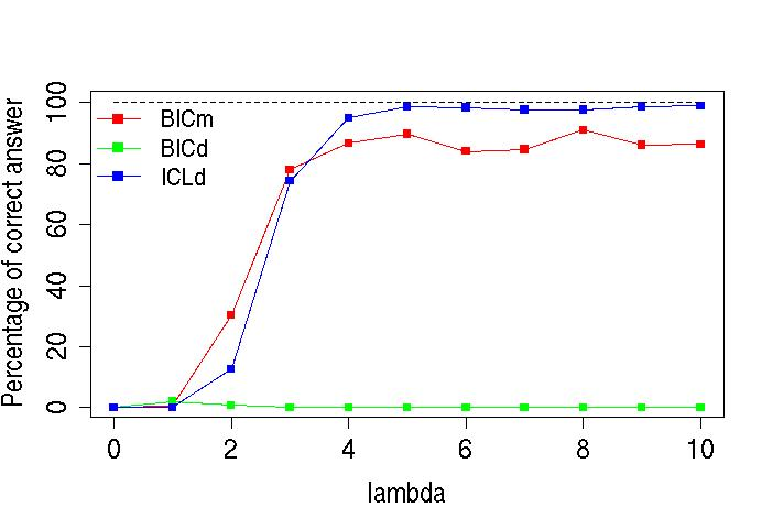
\epsfig{file=../Figures/ICLvsBIC.ps, clip=, bbllx=50, bblly=60,
          bburx=545, bbury=340, width=5cm, height=5cm} \\
        $\lambda_1 - \lambda_0$ ($\lambda_0 = 1$)
      \end{tabular}
    \end{column}
  \end{columns}
 }

%====================================================================
\frame{ \frametitle{Comments}
%====================================================================   
  \begin{itemize}
  \item \emphase{Exact computation} of BIC criteria can be achieved in
    $\Ocal(n^2)$.
  \item Either the dimension $K$ \emphase{or the segmentation} $m$ can
    be selected.
  \item Based on simulations, \emphase{BIC penalties seem too weak}
    (although there computation is exact).
  \item Interestingly, in the Gaussian case when using conjugate
    priors (Normal / inverse Gamma), the exact computation of $\log
    p(m |\Ybf)$ give raise to a term in
    $$
    \log \left(\prod_{r \in m} n_r\right)
    $$
    similar to the one of \refer{ZhS07}.
  \end{itemize}
  }

%====================================================================
\section{Mixed model for multiple profile}
\subsection{Multiple array analysis}
\frame{ \frametitle{Multiple array analysis}
%====================================================================   
  \begin{tabular}{cc}
    \begin{tabular}{p{6cm}}
      Cancer studies often involve CGH profiles of numerous
      patients ($q \approx 100$). \\
      \bigskip
      Even when having the same disease, patients generally
      \emphase{do not have common breakpoints}.\\
      \bigskip
      Simultaneous analysis of all profiles $\{Y_{it}\}$ allows
      to \emphase{correct for artifacts} such as probe effect.\\
        \bigskip
      \refer{PLB07}
    \end{tabular}    
    &
    \begin{tabular}{p{6cm}}
      \hspace{-.75cm}
      \epsfig{file = ../Figures/nakao-mat.txt-MixSeg-V2.eps, bbllx=90,
      bblly=220, bburx=380, bbury=590, clip=, scale=.5}
    \end{tabular}
  \end{tabular}
  }

%====================================================================
\frame{ \frametitle{Mixed segmentation model}
%==================================================================== 
  \emphase{Model.}
  \begin{itemize}
  \item Breakpoint positions are specific to each profile;
  \item Probe $t$ has a (random) effect that affects all profile at
    position $t$.
  \end{itemize}
  $$
  \text{if } (it) \in r, \quad Y_{it} = \mu_{ir} + U_t + E_{it}
  $$
  i.e.
  $$
  \Ybf = \Tbf \mubf + \Zbf \Ubf + \Ebf
  $$
  where 
  \begin{description}
  \item[$\Tbf =$] (unknown) segmentation matrix;
  \item[$\Zbf =$] design matrix of the probe effect;
  \item[$\Ubf =$] random (Gaussian) vector of probe effects;
  \item[$\Ebf =$] random (Gaussian) vector of residuals.
  \end{description}
  }

%====================================================================
\subsection{Estimation}
\frame{ \frametitle{Estimation via E-M}
%==================================================================== 
  \emphase{Direct maximisation.}
  Due to correlations, the variance matrix is not diagonal, so the
  log-likelihood is not additive over the segments \\
  \centerline{$\Rightarrow$ Dynamic programming \emphase{can not be applied}} \\
  \bigskip
  \emphase{A DP-EM algorithm.} \\
  The \emphase{conditional variance} of the $Y_{it}$ given $U$
  is diagonal, so DP can be used to estimate the breakpoints given
  $U$.
  \begin{description}
  \item[E-step.] Calculate the conditional moments of the
    random effect given the data:
    $$
    \widehat{\Esp}(U_t|Y_{it}), \qquad \widehat{\Var}(U_t|Y_{it}).
    $$
  \item[M-step.] Perform the segmentation of the 'corrected' signal:
    $$
    \widehat{\Tbf \mubf} = \arg\min_{\Tbf\mubf} \|\Ybf -
    {\Tbf\mubf}-\Zbf \widehat{\Ubf}\|^2.
    $$
    where $\widehat{\Ubf} = \widehat{\Esp}(\Ubf|\Ybf)$ ,
  \end{description}
  }

%====================================================================
\frame{ \frametitle{Practical implementation}
%==================================================================== 
  \emphase{Large dimension problem}
  \begin{itemize}
  \item When studying $q$ profiles, the M-step must achieve the
    segmentation of a signal with size $qn$.
  \item Quadratic complexity $\Ocal(q^2n^2)$ not manageable for large
    $q$ and $n$.
  \end{itemize}
  \bigskip
  \emphase{2-stage dynamic programming.} 
  \begin{enumerate}
  \item Segment each profile $i$ with number of breakpoints $K =
    1..K_\max$;
  \item The \emphase{optimal repartition} of the $K_i$'s between the
    $q$ profiles can be determined via dynamic programming.
  \end{enumerate}
  The total complexity is $\Ocal(qn^2)$.
  }

%====================================================================
\frame{ \frametitle{Bladder cancer data (F. Radvanyi, Curie)}
%==================================================================== 
  \vspace{-.5cm}
  \begin{tabular}{cc}
    \begin{tabular}{p{5cm}}
      Some large probe effect $U_t$ are detected\\
      $\rightarrow$ \emphase{Poor probe affinity}? \\
      $\rightarrow$ \emphase{Wrong annotation}? \\
      $\rightarrow$ \emphase{Polymorphism}? \\
      \bigskip
      Breakpoints near this position are likely to be artifacts. \\
      \bigskip
      The global segmentation is affected by this correction:\\
      \textcolor{red}{--}: independent segmentation, \\
      --: multivariate mixed segmentation.
    \end{tabular}
    &
    \hspace{-1cm}
    \begin{tabular}{c}
      \epsfig{file= ../FIGURES/Random_Effect.ps, clip=, 
        width=3cm, height=6.5cm, angle=270} \\
      \epsfig{file= ../FIGURES/Profils2_9_29.ps, width=6cm,
        height=2.5cm, clip=, bbllx=90, bblly=490, bburx=490, bbury=605} \\
      \epsfig{file= ../FIGURES/Profils2_9_29.ps, width=6cm,
        height=2.5cm, clip=, bbllx=90, bblly=210, bburx=490, bbury=335} 
    \end{tabular}
  \end{tabular}
  }

%====================================================================
\frame{ \frametitle{Multivariate segmentation ...}
%==================================================================== 
  \emphase{Package {\tt CGHseg}} available soon. \\
  \bigskip\bigskip
  Still some issues. \\
  \begin{description}
  \item[Interpretation of the probe effect], especially in
    case of recurrent alterations. \\
  \item[Classification of the segments] into 'deleted',
    'normal' and 'gain' status (\refer{PRL07}). \\
    Induces a second unknown structure (segment class + probe effect):
    \begin{itemize}
    \item Set a \emphase{fixed probe effect} $\rightarrow$ problem of
      convergence of the algorithm,
    \item Use \emphase{variational approximation} to deal with intricate
      dependencies.
    \end{itemize} \\
  \item[Model selection] for dependent signal (most sensitive point?)
  \end{description}
  }

%====================================================================
\section{Looking for recurrent alterations}
\subsection{Minimal regions}
\frame{ \frametitle{Looking for recurrent alterations}
%==================================================================== 
  \begin{tabular}{cc}
    \begin{tabular}{p{5cm}}
      To detect \emphase{alterations associated to a disease}
      (e.g. bladder cancer), we look for alterations that appear
      \emphase{'significantly'  often} among a set of patients.  \\ \\
      $X_{it}$ denotes the status of position $t$ for patient $i$:
      $$
      \begin{tabular}{rcrl}
        $X_{it}$ & = & \textcolor{blue}{--1} & \textcolor{blue}{(loss)} \\
        & = & 0 & (normal) \\
        & = & \textcolor{red}{+1} & \textcolor{red}{(gain)}
      \end{tabular}
      $$
      $i = 1..q, t = 1..n$.\\
      \refer{RSH06}
    \end{tabular}
    &
    \hspace{-.5cm}
    \begin{tabular}{c}
%       Recoded profiles into $\{-1, 0, +1\}$ \\
      \epsfig{file =
      /RECHERCHE/RUPTURES/Etudes/Curie/MinRegion/Data1/Profiles.eps,
      width=6.5cm, height=7cm, clip=} 
    \end{tabular}
  \end{tabular}
  }

%====================================================================
\frame{ \frametitle{Minimal region}
%==================================================================== 
  \begin{tabular}{cc}
    \begin{tabular}{p{7.5cm}}
      \emphase{Minimal region} = sequence of length $\ell$ for  which
        the \emphase{same status} is observed in \emphase{large 
        number} of patients $q^*$.\\ 
      \\
      \emphase{Data.} $q^* = 31$ patients have $\ell =
      5$ successive deletions between positions 1189 and 1193, in
      chromosome 9. \\
      (Bladder cancer data, F. Radvanyi, C. Rouveirol, Curie) \\
      \\
      \emphase{Question.} Is this significant, given
      \begin{itemize}
      \item the number of patients ($q=84$)
      \item the profiles length ($n=2340$)?
      \end{itemize}
    \end{tabular}
    &
    \begin{tabular}{c}
      \epsfig{file =
      /RECHERCHE/RUPTURES/Etudes/Curie/MinRegion/Data1/ExMinRegion.eps,
      clip=, bbllx=270, bblly=209, bburx=400, bbury=593, scale=.5} 
    \end{tabular}
  \end{tabular}
  }

%====================================================================
\frame{ \frametitle{Markov Model for Motif Statistics}
%==================================================================== 
  \emphase{Markov model (binary case).} Assume that only 2 status exist: 
  $$
  X_{it} = \left\{ 
    \begin{array}{rl}
      1 & \mbox{for alteration,} \\
      0 & \mbox{for normal.}
    \end{array}
  \right.
  \qquad
  \{X_{it}\}_t \text{ i.i.d. } \sim \text{MC}(\Pibf)
  $$
  
  \emphase{Region.} A minimal region is then a $\ell$-run of
  1s. Denote
  $$
  Y_{it} = \prod_{u=t-\ell+1}^t X_{it} = \left\{ 
    \begin{array}{rl}
      1 & \mbox{if a $\ell$-run occurs at position $t$ in profile $i$,} \\
      0 & \mbox{otherwise.}
    \end{array}
  \right.
  $$
  \emphase{Simultaneous occurrences.} $Y_{+t} = \sum_i Y_{it}$ is
  the number of patients for which a $\ell$ successive alterations
  (\emphase{$\ell$-run}) occurs at $t$.
  
  \bigskip
  \emphase{Significance of an observed minimal region.} We have to
  calculate 
  $$
  \Pr\left\{\max_{\ell \leq t \leq n}Y_{+t} \geq q^*\right\}.
  $$
  }

%====================================================================
\subsection{Significance}
\frame{ \frametitle{Significance: One profile}
%==================================================================== 
  \emphase{Waiting time.} What is the probability for a $\ell$-run to
  occur in a profile with length $n$
  $$
  \Pr\left\{\max_{\ell \leq t \leq n}Y_{t} \geq 1\right\} = \Pr\{ T
  \leq n\}
  $$
  where $T$ is the waiting time befor the first occurrence of a
  $\ell$-run. \\
  \bigskip   
  \emphase{Markov Chain embedding.}  We define $\{Z_t\}$, the Markov
  chain over $\{0, \dots, \ell\}$ describing the construction of a
  $\ell$-run; $\{Z_t\}$ has transition matrix
  $$
  {\small
    \Pbf = \left(
      \begin{array}{c|cccccc}
        & 0 & 1 & 2 & \dots & \ell-1 & \ell \\
        \hline
        0 & \pi_{00} & \pi_{01} \\
        1 & \pi_{10} & & \pi_{11} \\
        2 & \pi_{10} & & & \pi_{11} \\
        \vdots & \vdots & & & & \ddots \\
        \vdots & \pi_{10} & & & & & \pi_{11} \\
        \ell & & & & & & 1 \\
      \end{array}
    \right)
    }
  $$
  }

%====================================================================
\frame{ \frametitle{}
%==================================================================== 
  \emphase{Distribution of $Z_t$.} If the profile $\{X_t\}$ starts
  in the normal state ($X_1 = 0$), we have
  $$
  \mubf_1 = [1 \;  0 \; \dots \; 0]
  $$
  the distribution of $Z_t$ is given by 
  $$
  \mubf_t =  \mubf_1 \Pbf^{t-1}.
  $$
  \bigskip
  \emphase{Distribution of $T$.} Noting that
  $$
  \Pr\{T \leq n\} = \Pr\{Z_n = \ell\}
  $$
  the distribution of $T$ is given by the last coordinate of
  $\mubf_n$:
  $$
  \Pr\{T \leq n\} = \mu_{n, \ell}.
  $$
}

%====================================================================
\frame{ \frametitle{Significance: $q$ profiles}
%==================================================================== 
  We want to calculate $\displaystyle{ \Pr\left\{\max_{\ell \leq t
        \leq n}Y_{+t} \geq
      M^*\right\}}. $ \\
  \bigskip \emphase{Exact calculation.}  We consider $q$ independent
  Markov chains of order $\ell-1$:
  \\
  \centerline{$q = 84, \quad \ell = 15 \quad \rightarrow \quad 8.3\;
    10^{86}$ states...} \\
  \bigskip \emphase{Upper bound.}  Denoting $X_{+t} = \sum_i X_{it}$,
  we have
  $$
  \Pr\left\{\max_{\ell \leq t \leq n}Y_{+t} \geq q^*\right\} \leq
  \Pr\{X_{+t}, X_{+, t+1}, \dots X_{+, t+\ell-1} \geq q^*\}.
  $$
  $\{X_{+t}\}$ is a Markov chain, so the latter
  probability can be calculated via an \emphase{embedded Markov
    Chain}.  \\
  \bigskip
  \refer{RoS08} 
  }

%====================================================================
\frame{ \frametitle{}
%==================================================================== 
  \emphase{Embedded MC.} We define the MC 
  \begin{itemize}
  \item that counts successive positions where $X_{+t}$ exceeds $q^*$,
  \item with an \emphase{absorbing state} when this number reaches
    $\ell$. 
  \end{itemize}
  \bigskip \hspace{-.5cm}
  \begin{tabular}{ll}
    \begin{tabular}{p{4.5cm}}    
      The embedded MC has
      $$
      (q+1) + (\ell-2)(q-q^*+1) + 1
      $$ 
      states. \\ \\
      \emphase{Example.} \\
      $q = 84$, $\ell = 5$, $q^* = 31$, \\
      $\rightarrow$ 248 states. \\ \\
    \end{tabular}
    &      
    \hspace{-.5cm}
    $
    \Pbf = \left(
      \begin{tabular}{c}
        \epsfig{file=../Figures/ExPiR.eps, width=5cm, clip=}
      \end{tabular}
    \right)
    $
  \end{tabular}
  }

%====================================================================
\frame{ \frametitle{Loss regions in bladder cancer data}
%==================================================================== 
  $$
  {\small
    \begin{tabular}{cccccc}
      position &  & length & \# patients &
      \multicolumn{2}{c}{Significance} \\
      $t^*$  &  chrom.  &  $\ell$  &  $M^*$  &  $p$(upper)  &  $p$(lower) \\ 
\hline 
1189 & 9 & 5 & 31 & 6.04\;e--8 & 4.05\;e--8 \\ 
1387 & 11 & 3 & 30 & 6.82\;e--7 & 6.08\;e--7 \\ 
1430 & 11 & 3 & 27 & 5.08\;e--5 & 4.60\;e--5 \\ 
1340 & 10 & 22 & 23 & 1.18\;e--4 & 3.02\;e--6 \\ 
1457 & 11 & 3 & 26 & 1.91\;e--4 & 1.74\;e--4 \\ 
1006 & 8 & 42 & 21 & 4.95\;e--4 & 1.86\;e--8 \\ 
996 & 8 & 7 & 22 & 7.85\;e--3 & 4.78\;e--3 \\ 
584 & 4 & 6 & 19 & 1.82\;e--1 & 1.39\;e--1 \\ 
1947 & 17 & 26 & 16 & 2.33\;e--1 & 1.42\;e--2 \\ 
594 & 4 & 17 & 17 & 2.34\;e--1 & 5.16\;e--2 \\ 
643 & 5 & 11 & 17 & 4.18\;e--1 & 2.21\;e--1 \\ 

    \end{tabular} 
    } 
  $$
  \begin{itemize}
  \item The \emphase{upper and lower bounds are close},
    except for long regions.
  \item Some deletions (several in chrom. 9, gene TP53
    in chrom. 17) are \emphase{known to be associated to bladder cancer}.
  \end{itemize}
  }

%====================================================================
\frame{ \frametitle{Acknowledgements}
%==================================================================== 
  \begin{description}
  \item[Distribution over the segmentation space:]~\\
    G. Rigaill, E. Lebarbier \\
  \item[Mixed model for multiple profile:] ~\\
    F. Picard, E. Lebarbier, E. Budinska, B. Thiam \\
  \item[Looking for recurrent alterations:] ~\\
    V. Stefanov
  \item[Biology / Bioinformatics:] ~\\
    F. Radvanyi, C. Rouveirol
  \end{description}
    }

%====================================================================
\frame{ \frametitle{References}
%==================================================================== 
%     \bibliography{/biblio/AST,/biblio/ARC}
%     \bibliographystyle{/latex/astats}
%   \documentclass{beamer}

% Beamer style
%\usetheme[secheader]{Madrid}
\usetheme{CambridgeUS}
\usecolortheme[rgb={0.65,0.15,0.25}]{structure}
%\usefonttheme[onlymath]{serif}
\beamertemplatenavigationsymbolsempty
%\AtBeginSubsection

% Packages
%\usepackage[french]{babel}
\usepackage[latin1]{inputenc}
\usepackage{color}
\usepackage{dsfont, stmaryrd}
\usepackage{amsmath, amsfonts, amssymb}
\usepackage{epsfig}
\usepackage{/Latex/astats}
%\usepackage[all]{xy}
\usepackage{graphicx}

% Commands
\definecolor{darkred}{rgb}{0.65,0.15,0.25}
\newcommand{\emphase}[1]{\textcolor{darkred}{#1}}
\newcommand{\refer}[1]{\textcolor{blue}{\sl \cite{#1}}}

% Symbols
\newcommand{\BIC}{\text{BIC}}
\newcommand{\dd}{\text{d}}
\newcommand{\Esp}{\mathbb{E}}
\newcommand{\Ebf}{{\bf E}}
\newcommand{\ICL}{\text{ICL}}
\newcommand{\Cov}{\mathbb{C}\text{ov}}
\newcommand{\Var}{\mathbb{V}}
\newcommand{\pen}{\text{pen}}
\newcommand{\Hcal}{\text{H}}
\newcommand{\Lcal}{\mathcal{L}}
\newcommand{\Mcal}{\mathcal{M}}
\newcommand{\Ncal}{\mathcal{N}}
\newcommand{\Ocal}{\mathcal{O}}
\newcommand{\Pbf}{{\bf P}}
\newcommand{\Pcal}{\mathcal{P}}
\newcommand{\Vcal}{\mathcal{V}}
\newcommand{\Tbf}{{\bf T}}
\newcommand{\Ubf}{{\bf U}}
\newcommand{\Ybf}{{\bf Y}}
\newcommand{\Zbf}{{\bf Z}}
\newcommand{\Pibf}{\mbox{\mathversion{bold}{$\Pi$}}}
\newcommand{\mubf}{\mbox{\mathversion{bold}{$\mu$}}}
\newcommand{\thetabf}{\mbox{\mathversion{bold}{$\theta$}}}


%====================================================================
\title[Breakpoint detection \& CGH arrays]{Breakpoint detection and
  CGH arrays analysis}

\author{S. Robin}

\institute[AgroParisTech / INRA]{AgroParisTech / INRA \\
  \bigskip
  \begin{tabular}{ccccc}
    
\epsfig{file=../Figures/LogoINRA-Couleur.ps, width=2.5cm} &
    \hspace{.5cm} &
    
\epsfig{file=../Figures/logagroptechsolo.eps, width=3.75cm} &
    \hspace{.5cm} &
    \epsfig{file=../Figures/Logo-SSB.eps, width=2.5cm} \\
  \end{tabular} \\
  \bigskip
  }

\date[May '09]{SFdS, Bordeaux, May 2009}
%====================================================================

%====================================================================
%====================================================================
\begin{document}
%====================================================================
%====================================================================

%====================================================================
\frame{\titlepage}
%====================================================================

%====================================================================
\frame{ \frametitle{Outline}
%====================================================================
  
  \tableofcontents
%  \tableofcontents[pausesections]
  }

%====================================================================
\section{CGH for the detection of genomic alterations}
\subsection{Genomic alterations}
\frame{ \frametitle{Chromosomic alterations}
%==================================================================== 
  \begin{itemize}
  \item Known effects of big size chromosomal alterations (ex:
    trisomy).
  \item \emphase{Karyotype:} resolution $\sim$ chromosome)
    $$
    \epsfig{file = ../Figures/Karyotype.ps, clip=,
      bbllx=158, bblly=560, bburx=452, bbury=778, scale=.8}
    $$
  \end{itemize}
  }

%====================================================================
\frame{ \frametitle{Genomic alterations in cancer cells}
%==================================================================== 
  Genomic alterations are associated with (responsible for?) various
  types of cancers.
  $$
  \begin{tabular}{cc}
    Normal cell & Tumour cell \\
    \epsfig{file = ../Figures/KaryotypeCancer-PH.ps, clip=,
        bbllx=325, bblly=676, bburx=468, bbury=780, scale=.9}
    &
      \epsfig{file = ../Figures/KaryotypeCancer-PH.ps, clip=,
        bbllx=127, bblly=676, bburx=319, bbury=780, scale=.9}
    \end{tabular}
  $$
  \refer{Hup08} %\refer{Hup�}{08}
  }

%====================================================================
\subsection{CGH technology}
\frame{ \frametitle{CGH array technology}
%==================================================================== 
  Comparative Genomic Hybridisation = hybridisation of 2 DNA samples
  (\textcolor{red}{test} / \textcolor{green}{reference}) on a same
  chip. 
  $$
  \epsfig{file = ../Figures/principe_CGH.eps, clip=,
    bbllx=0, bblly=61, bburx=700, bbury=478, scale=0.4}
  $$
  \refer{Pic05}
  }

%====================================================================
\frame{ \frametitle{A segmentation problem}
%==================================================================== 
  \begin{tabular}{ccccc}
    \multicolumn{3}{c}{Zoom on CGH profile} & \quad & Karyotype \\
    chrom. 1 & \quad & chrom. 17 \\
                                %   \epsfig{file = ../Figures/Karyotype-CGH-PH.ps, clip=,
                                %     bbllx=80, bblly=617, bburx=150, bbury=763, scale=2}
    \epsfig{file = ../Figures/Karyotype-CGH-PH.ps, clip=,
      bbllx=80, bblly=617, bburx=150, bbury=700, scale=1.5}
    & &
                                %   \epsfig{file = ../Figures/Karyotype-CGH-PH.ps, clip=,
                                %     bbllx=270, bblly=617, bburx=300, bbury=763, scale=2}
    \epsfig{file = ../Figures/Karyotype-CGH-PH.ps, clip=,
      bbllx=270, bblly=617, bburx=300, bbury=700, scale=1.5}
    & &
    \epsfig{file = ../Figures/Karyotype-CGH-PH.ps, clip=,
      bbllx=364, bblly=617, bburx=485, bbury=763, scale=1}
  \end{tabular}

  \refer{Hup08}
  }

%====================================================================
\section{Distribution over the segmentation space}
\subsection{Change-point model}
\frame{ \frametitle{Change-point model}
%==================================================================== 
  \emphase{Notations:}
  \begin{itemize}
  \item $K = $ number of segments
  \item $r = $ region $\llbracket \tau_r, \tau^r \rrbracket$; $n_r =$
    length of $r$
  \item $m = $ segmentation: $m = \{r_1, \dots, r_K: \tau_{r+1} =
    \tau^r +1\}$
  \item $Y_t = $ signal at position $t$ ($t \in \llbracket 1, n
    \rrbracket$); $\Ybf = \{Y_t\}$.
  \end{itemize}
  \bigskip
  \emphase{Model:}
  \begin{itemize}
  \item $\{Y_t\}$ independent
  \item $t \in r$: 
    $$
    Y_t \sim p(\cdot | \theta_r)
    $$
  e.g. 
  $$
  p(\cdot|\theta_r) = \Ncal(\mu_r, \sigma^2), \qquad \Ncal(\mu_r,
  \sigma^2_r), \qquad \Pcal(\lambda_r)
  $$
  \end{itemize}
  \refer{PRL05}
  }

%====================================================================
\frame{ \frametitle{Optimal segmentation}
%==================================================================== 
  For a given dimension $K$, the maximum likelihood estimate (MLE) is
  $$
  (\widehat{m}(K), \widehat{\thetabf}(m)) = \underset{m \in
    \Mcal_K, \thetabf}{\arg\max} \; p(\Ybf | m, \thetabf)
  $$
  where $\Mcal_K$ is the set of all segmentations with dimension $K$:
  $$
  |\Mcal_K| = \binom{n-1}{K-1}
  $$
  \begin{itemize}
  \item \emphase{Exhaustive search} among $\Mcal_K$ can not be
    achieved.
  \item \emphase{Dynamic programming} provides $(\widehat{m},
    \widehat{\thetabf})$ with complexity $\Ocal(n^2)$.  
%     in both homoscedastic and heteroscedastic cases.
  \end{itemize}
  }

%====================================================================
\subsection{Model selection}
\frame{ \frametitle{Choice of $K$: Penalised contrast}
%==================================================================== 
  \emphase{2-step strategy.} 
  \begin{enumerate}
  \item Best segmentation with dimension $K$
    $$
    \widehat{m}(K) = \arg\min_{m \in \Mcal_K} \ell(\Ybf, m)
    $$
  \item Best dimension $K$
    $$
    \widehat{K} = \arg\min_{K} \ell(\Ybf, \widehat{m}(K)) + \pen(K)
    $$
  \end{enumerate}
  \refer{Leb05}: 
  $$\pen(K) = f(|\Mcal_K|);$$
  \refer{Lav05}: 
  $$\pen(K) = \beta K.$$
  \begin{itemize} 
  \item \emphase{Constant penalty} within each dimension $\Mcal_K$.
  \item The best model \emphase{$\widehat{m}(K)$ does not depend} on
    the penalty $\pen(K)$.
  \end{itemize}
  }

%====================================================================
\frame{ \frametitle{Bayesian Information Criterion (BIC)}
%==================================================================== 
  Bayesian framework: \emphase{$\BIC(M) \approx \log p(M | \Ybf)$},
  based on the Laplace approximation:
  $$
  \log \int p(M, \theta | \Ybf) \dd \theta \approx \log p(M | \Ybf, \widehat{\theta})
  - \frac{\log n}2 \dim(M)
  $$
  \emphase{Segmentation context:  $\BIC(K)$}
  $$
  \Mcal_K = \bigcup_{m\ \in \Mcal_K} \text{span}(m)
  $$
  \begin{itemize}
  \item Regularity conditions \emphase{not fulfilled} when 'model' $M$
    $=$ dimension $K$.
  \item \refer{ZhS07}: \emphase{modified approximation}
    $$
    \pen(K) = f(|\Mcal_K|) + g\left(\emphase{\sum_{r \in \widehat{m}(K)}
        \log n_r}\right)
    $$
  \end{itemize}
  }

%====================================================================
\frame{ \frametitle{Bayesian framework}
%==================================================================== 
  \begin{description}
  \item[$p(K) = $] prior of dimension $K$;
  \item[$p(m|K) = $] prior of segmentation $m$ given dimension $K$,
    $$
    \text{e.g.} \qquad
    p(m|K) = 1 \left/ |\Mcal_K| \right.
    $$
    that is, \emphase{uniform prior} within each dimension;
  \item[$p(m) = $] prior of segmentation $m$,
    $$
    \text{e.g.} \qquad
    p(m) \propto \prod_{r \in m} n_r
    $$
    that favours \emphase{regularly spaced} change-points
    ($\rightarrow$ implicit prior on $K$);
  \item[$p(\theta|m) =$] prior of $\theta$ given segmentation $m$.
  \end{description}
  }

%====================================================================
\frame{ \frametitle{Exact BIC criteria}
%==================================================================== 
  \emphase{Choice of $K$.}
  $$
  \BIC(K) = \log p(\Ybf, K) = \log \left[\emphase{\sum_{m \in
        \Mcal_K}} p(m) \int p(\Ybf | m, \theta) p(\theta |m) \dd
    \theta \right].
  $$
  \emphase{Choice of $m$.}
  $$
  \BIC(m) = \log p(\Ybf, m) = \log \left[p(m) \int p(\Ybf | m,
    \theta) p(\theta |m) \dd \theta \right]
  $$
  where $p(m)$ must normalised so that
  $$
  \sum_K \emphase{\sum_{m \in \Mcal_K}} p(m) = 1.
  $$
  }

%====================================================================
\frame{ \frametitle{2 hypotheses}
%==================================================================== 
  \begin{enumerate}
  \item \emphase{Factorisation:}
    $$
    p(m) = \prod_{r \in m} f(r), 
    \quad
    p(\theta|m) = \prod_{r \in m} f(\theta_r) 
    \quad
    p(\Ybf|m, \theta) = \prod_{r \in m} f(Y^r, \theta_r) 
    $$
    (not true for homoscedastic models), so sums can be rewritten as
    $$
    \sum_{m \in \Mcal_K} f(m) = \sum_{m \in \Mcal_K} \prod_{r \in m} f(r)
    $$
  \item \bigskip \emphase{Conjugate priors.} $\theta^0_r =$ parameter
    of the prior $p(\theta_r)$
    $$
    f(Y^r; \theta^0_r) = \int p(Y^r|\theta_r) p(\theta_r; \theta^0_r) \dd_r
    \quad \text{has an explicit form.}
    $$
    Avoids the Laplace approximation: \\
    $\rightarrow$ regularity conditions \emphase{are fulfilled} for
    any segmentation $m$, \\
    $\rightarrow$ but the asymptotic framework does not apply to small regions.
  \end{enumerate}
  }

%====================================================================
\frame{ \frametitle{Exploring the segmentation space}
%==================================================================== 
  \framebox{\begin{tabular}{l} 
      \emphase{Proposition.}  All terms $\sum_{m \in \Mcal_K} \prod_{r
      \in m} g(m)$ can be computed in a\\ 
      quadratic time $\Ocal(n^2)$.
    \end{tabular}} \\
    \bigskip \emphase{Idea:} Whatever the dimension $K$, there is only
    a
    quadratic number of regions $r$. \\
    \bigskip
  \begin{itemize}
  \item Similar to an algorithm proposed by \refer{Gue07} in the HMM
    context with known parameters.
  \item Allows to compute various quantities, including the
    \emphase{posterior entropy of $m$} within a dimension:
    $$
    \Hcal(K) = - \sum_{m \in \Mcal_K} p(m|\Ybf, K) \log p(m|\Ybf, K) 
    $$
    (\emphase{see G. Rigaill's talk})
  \end{itemize}
 }

%====================================================================
\frame{ \frametitle{ICL criterion}
%==================================================================== 
  \emphase{Incomplete data model context} (mixture model):
  \begin{itemize}
  \item \refer{BCG00} add an entropy term $\Hcal(K)$ to the $\BIC(K)$
    penalty
  \item $\Hcal(K)$ accounts for the reliability of the prediction of
    the unknown variable.
  \end{itemize}
  \bigskip 
  \emphase{Segmentation context.}
  \begin{itemize}
  \item Change-point positions can be view as unknown variables.
  \item For a given dimension $K$, it is desirable that the best
    segmentation clearly outperforms the others:
    $$
    \text{for any } m \in \Mcal_K \setminus \{\widehat{m}(K)\}:
    \quad p(\widehat{m}(K)|\Ybf) \gg p(m | \Ybf).
    $$
  \item This can be measured by the posterior entropy $\Hcal(K)$
  \end{itemize}
  \bigskip
  \emphase{ICL criterion:}
  $$
  \ICL(K) = \log \sum_{m \in \Mcal_K} p(\Ybf, m) - \Hcal(K)
  $$
    }

%====================================================================
\frame{ \frametitle{}
%==================================================================== 
  \vspace{-1cm}
  $$
  \begin{tabular}{cc}
    \begin{tabular}{c}
      \emphase{Example} \\
      \epsfig{file=../Figures/CopyNumberChr1_Alone.ps, 
        bbllx=38, bblly=40, bburx=565, bbury=385, width=4.25cm, height=2.25cm,
        clip=} \\
      \\
      $\BIC(K)$ \\
      \epsfig{file = ../FIGURES/BIC2_NP.ps, width=5cm, height=2.5cm,
        clip=} \\
    \end{tabular}
    &
    \begin{tabular}{c}
%       \\
%       $\ICL(K) = f[\BIC(K)]$ \\
%       \epsfig{file=../Figures//BICandEntropy.ps, clip=, scale=0.25,
%         bbllx=38, bblly=40, bburx=565, bbury=385}
      $\BIC(m)$ \\
      \epsfig{file = ../FIGURES/BIC_NP.ps, width=5cm, height=2.5cm,
        clip=} \\
      \\
      $\ICL(K)$ \\
      \epsfig{file = ../FIGURES/ICL_NP.ps, width=5cm, height=2.5cm,
        clip=} \\
    \end{tabular}
  \end{tabular}
  $$
  When $K$ exceeds the 'true' dimension, all segmentations
  nested within the 'true' one have a high posterior probability,
  which increases the entropy. 
}

%====================================================================
\frame{ \frametitle{Comparison BIC/ICL}
%==================================================================== 
  \begin{columns}
    \begin{column}{0.45\linewidth}
      \emphase{Simulations: } Poisson signal with alternating
      means $\lambda_0$ and $\lambda_1$, $n = 100$. \\
      \bigskip \emphase{Criterion} = \% of recovery of the true number
      of segments ($K =
      5$). \\
      \bigskip
      \begin{itemize}
      \item $\BIC(m)$ achieves (much) better performances than
        $\BIC(K)$
      \item $\ICL(K)$ outperforms both $\BIC(K)$ and $\BIC(m)$.
      \end{itemize}
    \end{column}
    
    \begin{column}{0.45\linewidth}
      \begin{tabular}{c}
        \textcolor{green}{$\BIC(K)$} \quad \textcolor{red}{$\BIC(m)$} \quad
        \textcolor{blue}{$\ICL(K)$} \\
        ~\\
        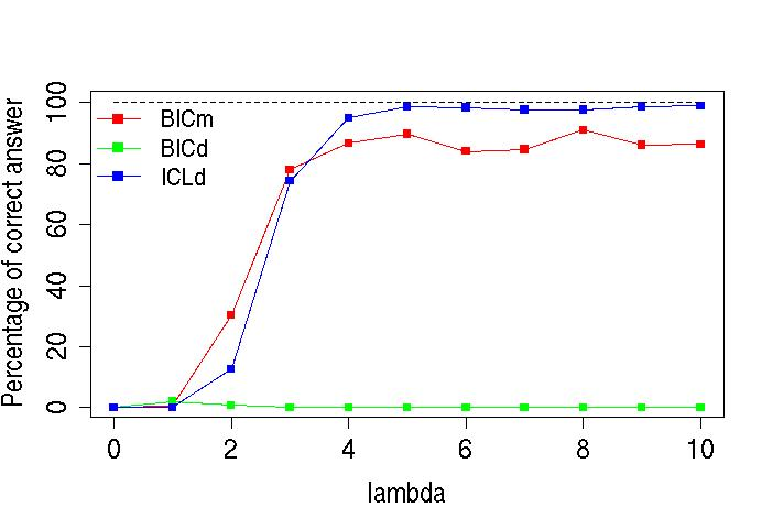
\epsfig{file=../Figures/ICLvsBIC.ps, clip=, bbllx=50, bblly=60,
          bburx=545, bbury=340, width=5cm, height=5cm} \\
        $\lambda_1 - \lambda_0$ ($\lambda_0 = 1$)
      \end{tabular}
    \end{column}
  \end{columns}
 }

%====================================================================
\frame{ \frametitle{Comments}
%====================================================================   
  \begin{itemize}
  \item \emphase{Exact computation} of BIC criteria can be achieved in
    $\Ocal(n^2)$.
  \item Either the dimension $K$ \emphase{or the segmentation} $m$ can
    be selected.
  \item Based on simulations, \emphase{BIC penalties seem too weak}
    (although there computation is exact).
  \item Interestingly, in the Gaussian case when using conjugate
    priors (Normal / inverse Gamma), the exact computation of $\log
    p(m |\Ybf)$ give raise to a term in
    $$
    \log \left(\prod_{r \in m} n_r\right)
    $$
    similar to the one of \refer{ZhS07}.
  \end{itemize}
  }

%====================================================================
\section{Mixed model for multiple profile}
\subsection{Multiple array analysis}
\frame{ \frametitle{Multiple array analysis}
%====================================================================   
  \begin{tabular}{cc}
    \begin{tabular}{p{6cm}}
      Cancer studies often involve CGH profiles of numerous
      patients ($q \approx 100$). \\
      \bigskip
      Even when having the same disease, patients generally
      \emphase{do not have common breakpoints}.\\
      \bigskip
      Simultaneous analysis of all profiles $\{Y_{it}\}$ allows
      to \emphase{correct for artifacts} such as probe effect.\\
        \bigskip
      \refer{PLB07}
    \end{tabular}    
    &
    \begin{tabular}{p{6cm}}
      \hspace{-.75cm}
      \epsfig{file = ../Figures/nakao-mat.txt-MixSeg-V2.eps, bbllx=90,
      bblly=220, bburx=380, bbury=590, clip=, scale=.5}
    \end{tabular}
  \end{tabular}
  }

%====================================================================
\frame{ \frametitle{Mixed segmentation model}
%==================================================================== 
  \emphase{Model.}
  \begin{itemize}
  \item Breakpoint positions are specific to each profile;
  \item Probe $t$ has a (random) effect that affects all profile at
    position $t$.
  \end{itemize}
  $$
  \text{if } (it) \in r, \quad Y_{it} = \mu_{ir} + U_t + E_{it}
  $$
  i.e.
  $$
  \Ybf = \Tbf \mubf + \Zbf \Ubf + \Ebf
  $$
  where 
  \begin{description}
  \item[$\Tbf =$] (unknown) segmentation matrix;
  \item[$\Zbf =$] design matrix of the probe effect;
  \item[$\Ubf =$] random (Gaussian) vector of probe effects;
  \item[$\Ebf =$] random (Gaussian) vector of residuals.
  \end{description}
  }

%====================================================================
\subsection{Estimation}
\frame{ \frametitle{Estimation via E-M}
%==================================================================== 
  \emphase{Direct maximisation.}
  Due to correlations, the variance matrix is not diagonal, so the
  log-likelihood is not additive over the segments \\
  \centerline{$\Rightarrow$ Dynamic programming \emphase{can not be applied}} \\
  \bigskip
  \emphase{A DP-EM algorithm.} \\
  The \emphase{conditional variance} of the $Y_{it}$ given $U$
  is diagonal, so DP can be used to estimate the breakpoints given
  $U$.
  \begin{description}
  \item[E-step.] Calculate the conditional moments of the
    random effect given the data:
    $$
    \widehat{\Esp}(U_t|Y_{it}), \qquad \widehat{\Var}(U_t|Y_{it}).
    $$
  \item[M-step.] Perform the segmentation of the 'corrected' signal:
    $$
    \widehat{\Tbf \mubf} = \arg\min_{\Tbf\mubf} \|\Ybf -
    {\Tbf\mubf}-\Zbf \widehat{\Ubf}\|^2.
    $$
    where $\widehat{\Ubf} = \widehat{\Esp}(\Ubf|\Ybf)$ ,
  \end{description}
  }

%====================================================================
\frame{ \frametitle{Practical implementation}
%==================================================================== 
  \emphase{Large dimension problem}
  \begin{itemize}
  \item When studying $q$ profiles, the M-step must achieve the
    segmentation of a signal with size $qn$.
  \item Quadratic complexity $\Ocal(q^2n^2)$ not manageable for large
    $q$ and $n$.
  \end{itemize}
  \bigskip
  \emphase{2-stage dynamic programming.} 
  \begin{enumerate}
  \item Segment each profile $i$ with number of breakpoints $K =
    1..K_\max$;
  \item The \emphase{optimal repartition} of the $K_i$'s between the
    $q$ profiles can be determined via dynamic programming.
  \end{enumerate}
  The total complexity is $\Ocal(qn^2)$.
  }

%====================================================================
\frame{ \frametitle{Bladder cancer data (F. Radvanyi, Curie)}
%==================================================================== 
  \vspace{-.5cm}
  \begin{tabular}{cc}
    \begin{tabular}{p{5cm}}
      Some large probe effect $U_t$ are detected\\
      $\rightarrow$ \emphase{Poor probe affinity}? \\
      $\rightarrow$ \emphase{Wrong annotation}? \\
      $\rightarrow$ \emphase{Polymorphism}? \\
      \bigskip
      Breakpoints near this position are likely to be artifacts. \\
      \bigskip
      The global segmentation is affected by this correction:\\
      \textcolor{red}{--}: independent segmentation, \\
      --: multivariate mixed segmentation.
    \end{tabular}
    &
    \hspace{-1cm}
    \begin{tabular}{c}
      \epsfig{file= ../FIGURES/Random_Effect.ps, clip=, 
        width=3cm, height=6.5cm, angle=270} \\
      \epsfig{file= ../FIGURES/Profils2_9_29.ps, width=6cm,
        height=2.5cm, clip=, bbllx=90, bblly=490, bburx=490, bbury=605} \\
      \epsfig{file= ../FIGURES/Profils2_9_29.ps, width=6cm,
        height=2.5cm, clip=, bbllx=90, bblly=210, bburx=490, bbury=335} 
    \end{tabular}
  \end{tabular}
  }

%====================================================================
\frame{ \frametitle{Multivariate segmentation ...}
%==================================================================== 
  \emphase{Package {\tt CGHseg}} available soon. \\
  \bigskip\bigskip
  Still some issues. \\
  \begin{description}
  \item[Interpretation of the probe effect], especially in
    case of recurrent alterations. \\
  \item[Classification of the segments] into 'deleted',
    'normal' and 'gain' status (\refer{PRL07}). \\
    Induces a second unknown structure (segment class + probe effect):
    \begin{itemize}
    \item Set a \emphase{fixed probe effect} $\rightarrow$ problem of
      convergence of the algorithm,
    \item Use \emphase{variational approximation} to deal with intricate
      dependencies.
    \end{itemize} \\
  \item[Model selection] for dependent signal (most sensitive point?)
  \end{description}
  }

%====================================================================
\section{Looking for recurrent alterations}
\subsection{Minimal regions}
\frame{ \frametitle{Looking for recurrent alterations}
%==================================================================== 
  \begin{tabular}{cc}
    \begin{tabular}{p{5cm}}
      To detect \emphase{alterations associated to a disease}
      (e.g. bladder cancer), we look for alterations that appear
      \emphase{'significantly'  often} among a set of patients.  \\ \\
      $X_{it}$ denotes the status of position $t$ for patient $i$:
      $$
      \begin{tabular}{rcrl}
        $X_{it}$ & = & \textcolor{blue}{--1} & \textcolor{blue}{(loss)} \\
        & = & 0 & (normal) \\
        & = & \textcolor{red}{+1} & \textcolor{red}{(gain)}
      \end{tabular}
      $$
      $i = 1..q, t = 1..n$.\\
      \refer{RSH06}
    \end{tabular}
    &
    \hspace{-.5cm}
    \begin{tabular}{c}
%       Recoded profiles into $\{-1, 0, +1\}$ \\
      \epsfig{file =
      /RECHERCHE/RUPTURES/Etudes/Curie/MinRegion/Data1/Profiles.eps,
      width=6.5cm, height=7cm, clip=} 
    \end{tabular}
  \end{tabular}
  }

%====================================================================
\frame{ \frametitle{Minimal region}
%==================================================================== 
  \begin{tabular}{cc}
    \begin{tabular}{p{7.5cm}}
      \emphase{Minimal region} = sequence of length $\ell$ for  which
        the \emphase{same status} is observed in \emphase{large 
        number} of patients $q^*$.\\ 
      \\
      \emphase{Data.} $q^* = 31$ patients have $\ell =
      5$ successive deletions between positions 1189 and 1193, in
      chromosome 9. \\
      (Bladder cancer data, F. Radvanyi, C. Rouveirol, Curie) \\
      \\
      \emphase{Question.} Is this significant, given
      \begin{itemize}
      \item the number of patients ($q=84$)
      \item the profiles length ($n=2340$)?
      \end{itemize}
    \end{tabular}
    &
    \begin{tabular}{c}
      \epsfig{file =
      /RECHERCHE/RUPTURES/Etudes/Curie/MinRegion/Data1/ExMinRegion.eps,
      clip=, bbllx=270, bblly=209, bburx=400, bbury=593, scale=.5} 
    \end{tabular}
  \end{tabular}
  }

%====================================================================
\frame{ \frametitle{Markov Model for Motif Statistics}
%==================================================================== 
  \emphase{Markov model (binary case).} Assume that only 2 status exist: 
  $$
  X_{it} = \left\{ 
    \begin{array}{rl}
      1 & \mbox{for alteration,} \\
      0 & \mbox{for normal.}
    \end{array}
  \right.
  \qquad
  \{X_{it}\}_t \text{ i.i.d. } \sim \text{MC}(\Pibf)
  $$
  
  \emphase{Region.} A minimal region is then a $\ell$-run of
  1s. Denote
  $$
  Y_{it} = \prod_{u=t-\ell+1}^t X_{it} = \left\{ 
    \begin{array}{rl}
      1 & \mbox{if a $\ell$-run occurs at position $t$ in profile $i$,} \\
      0 & \mbox{otherwise.}
    \end{array}
  \right.
  $$
  \emphase{Simultaneous occurrences.} $Y_{+t} = \sum_i Y_{it}$ is
  the number of patients for which a $\ell$ successive alterations
  (\emphase{$\ell$-run}) occurs at $t$.
  
  \bigskip
  \emphase{Significance of an observed minimal region.} We have to
  calculate 
  $$
  \Pr\left\{\max_{\ell \leq t \leq n}Y_{+t} \geq q^*\right\}.
  $$
  }

%====================================================================
\subsection{Significance}
\frame{ \frametitle{Significance: One profile}
%==================================================================== 
  \emphase{Waiting time.} What is the probability for a $\ell$-run to
  occur in a profile with length $n$
  $$
  \Pr\left\{\max_{\ell \leq t \leq n}Y_{t} \geq 1\right\} = \Pr\{ T
  \leq n\}
  $$
  where $T$ is the waiting time befor the first occurrence of a
  $\ell$-run. \\
  \bigskip   
  \emphase{Markov Chain embedding.}  We define $\{Z_t\}$, the Markov
  chain over $\{0, \dots, \ell\}$ describing the construction of a
  $\ell$-run; $\{Z_t\}$ has transition matrix
  $$
  {\small
    \Pbf = \left(
      \begin{array}{c|cccccc}
        & 0 & 1 & 2 & \dots & \ell-1 & \ell \\
        \hline
        0 & \pi_{00} & \pi_{01} \\
        1 & \pi_{10} & & \pi_{11} \\
        2 & \pi_{10} & & & \pi_{11} \\
        \vdots & \vdots & & & & \ddots \\
        \vdots & \pi_{10} & & & & & \pi_{11} \\
        \ell & & & & & & 1 \\
      \end{array}
    \right)
    }
  $$
  }

%====================================================================
\frame{ \frametitle{}
%==================================================================== 
  \emphase{Distribution of $Z_t$.} If the profile $\{X_t\}$ starts
  in the normal state ($X_1 = 0$), we have
  $$
  \mubf_1 = [1 \;  0 \; \dots \; 0]
  $$
  the distribution of $Z_t$ is given by 
  $$
  \mubf_t =  \mubf_1 \Pbf^{t-1}.
  $$
  \bigskip
  \emphase{Distribution of $T$.} Noting that
  $$
  \Pr\{T \leq n\} = \Pr\{Z_n = \ell\}
  $$
  the distribution of $T$ is given by the last coordinate of
  $\mubf_n$:
  $$
  \Pr\{T \leq n\} = \mu_{n, \ell}.
  $$
}

%====================================================================
\frame{ \frametitle{Significance: $q$ profiles}
%==================================================================== 
  We want to calculate $\displaystyle{ \Pr\left\{\max_{\ell \leq t
        \leq n}Y_{+t} \geq
      M^*\right\}}. $ \\
  \bigskip \emphase{Exact calculation.}  We consider $q$ independent
  Markov chains of order $\ell-1$:
  \\
  \centerline{$q = 84, \quad \ell = 15 \quad \rightarrow \quad 8.3\;
    10^{86}$ states...} \\
  \bigskip \emphase{Upper bound.}  Denoting $X_{+t} = \sum_i X_{it}$,
  we have
  $$
  \Pr\left\{\max_{\ell \leq t \leq n}Y_{+t} \geq q^*\right\} \leq
  \Pr\{X_{+t}, X_{+, t+1}, \dots X_{+, t+\ell-1} \geq q^*\}.
  $$
  $\{X_{+t}\}$ is a Markov chain, so the latter
  probability can be calculated via an \emphase{embedded Markov
    Chain}.  \\
  \bigskip
  \refer{RoS08} 
  }

%====================================================================
\frame{ \frametitle{}
%==================================================================== 
  \emphase{Embedded MC.} We define the MC 
  \begin{itemize}
  \item that counts successive positions where $X_{+t}$ exceeds $q^*$,
  \item with an \emphase{absorbing state} when this number reaches
    $\ell$. 
  \end{itemize}
  \bigskip \hspace{-.5cm}
  \begin{tabular}{ll}
    \begin{tabular}{p{4.5cm}}    
      The embedded MC has
      $$
      (q+1) + (\ell-2)(q-q^*+1) + 1
      $$ 
      states. \\ \\
      \emphase{Example.} \\
      $q = 84$, $\ell = 5$, $q^* = 31$, \\
      $\rightarrow$ 248 states. \\ \\
    \end{tabular}
    &      
    \hspace{-.5cm}
    $
    \Pbf = \left(
      \begin{tabular}{c}
        \epsfig{file=../Figures/ExPiR.eps, width=5cm, clip=}
      \end{tabular}
    \right)
    $
  \end{tabular}
  }

%====================================================================
\frame{ \frametitle{Loss regions in bladder cancer data}
%==================================================================== 
  $$
  {\small
    \begin{tabular}{cccccc}
      position &  & length & \# patients &
      \multicolumn{2}{c}{Significance} \\
      $t^*$  &  chrom.  &  $\ell$  &  $M^*$  &  $p$(upper)  &  $p$(lower) \\ 
\hline 
1189 & 9 & 5 & 31 & 6.04\;e--8 & 4.05\;e--8 \\ 
1387 & 11 & 3 & 30 & 6.82\;e--7 & 6.08\;e--7 \\ 
1430 & 11 & 3 & 27 & 5.08\;e--5 & 4.60\;e--5 \\ 
1340 & 10 & 22 & 23 & 1.18\;e--4 & 3.02\;e--6 \\ 
1457 & 11 & 3 & 26 & 1.91\;e--4 & 1.74\;e--4 \\ 
1006 & 8 & 42 & 21 & 4.95\;e--4 & 1.86\;e--8 \\ 
996 & 8 & 7 & 22 & 7.85\;e--3 & 4.78\;e--3 \\ 
584 & 4 & 6 & 19 & 1.82\;e--1 & 1.39\;e--1 \\ 
1947 & 17 & 26 & 16 & 2.33\;e--1 & 1.42\;e--2 \\ 
594 & 4 & 17 & 17 & 2.34\;e--1 & 5.16\;e--2 \\ 
643 & 5 & 11 & 17 & 4.18\;e--1 & 2.21\;e--1 \\ 

    \end{tabular} 
    } 
  $$
  \begin{itemize}
  \item The \emphase{upper and lower bounds are close},
    except for long regions.
  \item Some deletions (several in chrom. 9, gene TP53
    in chrom. 17) are \emphase{known to be associated to bladder cancer}.
  \end{itemize}
  }

%====================================================================
\frame{ \frametitle{Acknowledgements}
%==================================================================== 
  \begin{description}
  \item[Distribution over the segmentation space:]~\\
    G. Rigaill, E. Lebarbier \\
  \item[Mixed model for multiple profile:] ~\\
    F. Picard, E. Lebarbier, E. Budinska, B. Thiam \\
  \item[Looking for recurrent alterations:] ~\\
    V. Stefanov
  \item[Biology / Bioinformatics:] ~\\
    F. Radvanyi, C. Rouveirol
  \end{description}
    }

%====================================================================
\frame{ \frametitle{References}
%==================================================================== 
%     \bibliography{/biblio/AST,/biblio/ARC}
%     \bibliographystyle{/latex/astats}
%   \documentclass{beamer}

% Beamer style
%\usetheme[secheader]{Madrid}
\usetheme{CambridgeUS}
\usecolortheme[rgb={0.65,0.15,0.25}]{structure}
%\usefonttheme[onlymath]{serif}
\beamertemplatenavigationsymbolsempty
%\AtBeginSubsection

% Packages
%\usepackage[french]{babel}
\usepackage[latin1]{inputenc}
\usepackage{color}
\usepackage{dsfont, stmaryrd}
\usepackage{amsmath, amsfonts, amssymb}
\usepackage{epsfig}
\usepackage{/Latex/astats}
%\usepackage[all]{xy}
\usepackage{graphicx}

% Commands
\definecolor{darkred}{rgb}{0.65,0.15,0.25}
\newcommand{\emphase}[1]{\textcolor{darkred}{#1}}
\newcommand{\refer}[1]{\textcolor{blue}{\sl \cite{#1}}}

% Symbols
\newcommand{\BIC}{\text{BIC}}
\newcommand{\dd}{\text{d}}
\newcommand{\Esp}{\mathbb{E}}
\newcommand{\Ebf}{{\bf E}}
\newcommand{\ICL}{\text{ICL}}
\newcommand{\Cov}{\mathbb{C}\text{ov}}
\newcommand{\Var}{\mathbb{V}}
\newcommand{\pen}{\text{pen}}
\newcommand{\Hcal}{\text{H}}
\newcommand{\Lcal}{\mathcal{L}}
\newcommand{\Mcal}{\mathcal{M}}
\newcommand{\Ncal}{\mathcal{N}}
\newcommand{\Ocal}{\mathcal{O}}
\newcommand{\Pbf}{{\bf P}}
\newcommand{\Pcal}{\mathcal{P}}
\newcommand{\Vcal}{\mathcal{V}}
\newcommand{\Tbf}{{\bf T}}
\newcommand{\Ubf}{{\bf U}}
\newcommand{\Ybf}{{\bf Y}}
\newcommand{\Zbf}{{\bf Z}}
\newcommand{\Pibf}{\mbox{\mathversion{bold}{$\Pi$}}}
\newcommand{\mubf}{\mbox{\mathversion{bold}{$\mu$}}}
\newcommand{\thetabf}{\mbox{\mathversion{bold}{$\theta$}}}


%====================================================================
\title[Breakpoint detection \& CGH arrays]{Breakpoint detection and
  CGH arrays analysis}

\author{S. Robin}

\institute[AgroParisTech / INRA]{AgroParisTech / INRA \\
  \bigskip
  \begin{tabular}{ccccc}
    \epsfig{file=../Figures/LogoINRA-Couleur.ps, width=2.5cm} &
    \hspace{.5cm} &
    \epsfig{file=../Figures/logagroptechsolo.eps, width=3.75cm} &
    \hspace{.5cm} &
    \epsfig{file=../Figures/Logo-SSB.eps, width=2.5cm} \\
  \end{tabular} \\
  \bigskip
  }

\date[May '09]{SFdS, Bordeaux, May 2009}
%====================================================================

%====================================================================
%====================================================================
\begin{document}
%====================================================================
%====================================================================

%====================================================================
\frame{\titlepage}
%====================================================================

%====================================================================
\frame{ \frametitle{Outline}
%====================================================================
  
  \tableofcontents
%  \tableofcontents[pausesections]
  }

%====================================================================
\section{CGH for the detection of genomic alterations}
\subsection{Genomic alterations}
\frame{ \frametitle{Chromosomic alterations}
%==================================================================== 
  \begin{itemize}
  \item Known effects of big size chromosomal alterations (ex:
    trisomy).
  \item \emphase{Karyotype:} resolution $\sim$ chromosome)
    $$
    \epsfig{file = ../Figures/Karyotype.ps, clip=,
      bbllx=158, bblly=560, bburx=452, bbury=778, scale=.8}
    $$
  \end{itemize}
  }

%====================================================================
\frame{ \frametitle{Genomic alterations in cancer cells}
%==================================================================== 
  Genomic alterations are associated with (responsible for?) various
  types of cancers.
  $$
  \begin{tabular}{cc}
    Normal cell & Tumour cell \\
    \epsfig{file = ../Figures/KaryotypeCancer-PH.ps, clip=,
        bbllx=325, bblly=676, bburx=468, bbury=780, scale=.9}
    &
      \epsfig{file = ../Figures/KaryotypeCancer-PH.ps, clip=,
        bbllx=127, bblly=676, bburx=319, bbury=780, scale=.9}
    \end{tabular}
  $$
  \refer{Hup08} %\refer{Hup�}{08}
  }

%====================================================================
\subsection{CGH technology}
\frame{ \frametitle{CGH array technology}
%==================================================================== 
  Comparative Genomic Hybridisation = hybridisation of 2 DNA samples
  (\textcolor{red}{test} / \textcolor{green}{reference}) on a same
  chip. 
  $$
  \epsfig{file = ../Figures/principe_CGH.eps, clip=,
    bbllx=0, bblly=61, bburx=700, bbury=478, scale=0.4}
  $$
  \refer{Pic05}
  }

%====================================================================
\frame{ \frametitle{A segmentation problem}
%==================================================================== 
  \begin{tabular}{ccccc}
    \multicolumn{3}{c}{Zoom on CGH profile} & \quad & Karyotype \\
    chrom. 1 & \quad & chrom. 17 \\
                                %   \epsfig{file = ../Figures/Karyotype-CGH-PH.ps, clip=,
                                %     bbllx=80, bblly=617, bburx=150, bbury=763, scale=2}
    \epsfig{file = ../Figures/Karyotype-CGH-PH.ps, clip=,
      bbllx=80, bblly=617, bburx=150, bbury=700, scale=1.5}
    & &
                                %   \epsfig{file = ../Figures/Karyotype-CGH-PH.ps, clip=,
                                %     bbllx=270, bblly=617, bburx=300, bbury=763, scale=2}
    \epsfig{file = ../Figures/Karyotype-CGH-PH.ps, clip=,
      bbllx=270, bblly=617, bburx=300, bbury=700, scale=1.5}
    & &
    \epsfig{file = ../Figures/Karyotype-CGH-PH.ps, clip=,
      bbllx=364, bblly=617, bburx=485, bbury=763, scale=1}
  \end{tabular}

  \refer{Hup08}
  }

%====================================================================
\section{Distribution over the segmentation space}
\subsection{Change-point model}
\frame{ \frametitle{Change-point model}
%==================================================================== 
  \emphase{Notations:}
  \begin{itemize}
  \item $K = $ number of segments
  \item $r = $ region $\llbracket \tau_r, \tau^r \rrbracket$; $n_r =$
    length of $r$
  \item $m = $ segmentation: $m = \{r_1, \dots, r_K: \tau_{r+1} =
    \tau^r +1\}$
  \item $Y_t = $ signal at position $t$ ($t \in \llbracket 1, n
    \rrbracket$); $\Ybf = \{Y_t\}$.
  \end{itemize}
  \bigskip
  \emphase{Model:}
  \begin{itemize}
  \item $\{Y_t\}$ independent
  \item $t \in r$: 
    $$
    Y_t \sim p(\cdot | \theta_r)
    $$
  e.g. 
  $$
  p(\cdot|\theta_r) = \Ncal(\mu_r, \sigma^2), \qquad \Ncal(\mu_r,
  \sigma^2_r), \qquad \Pcal(\lambda_r)
  $$
  \end{itemize}
  \refer{PRL05}
  }

%====================================================================
\frame{ \frametitle{Optimal segmentation}
%==================================================================== 
  For a given dimension $K$, the maximum likelihood estimate (MLE) is
  $$
  (\widehat{m}(K), \widehat{\thetabf}(m)) = \underset{m \in
    \Mcal_K, \thetabf}{\arg\max} \; p(\Ybf | m, \thetabf)
  $$
  where $\Mcal_K$ is the set of all segmentations with dimension $K$:
  $$
  |\Mcal_K| = \binom{n-1}{K-1}
  $$
  \begin{itemize}
  \item \emphase{Exhaustive search} among $\Mcal_K$ can not be
    achieved.
  \item \emphase{Dynamic programming} provides $(\widehat{m},
    \widehat{\thetabf})$ with complexity $\Ocal(n^2)$.  
%     in both homoscedastic and heteroscedastic cases.
  \end{itemize}
  }

%====================================================================
\subsection{Model selection}
\frame{ \frametitle{Choice of $K$: Penalised contrast}
%==================================================================== 
  \emphase{2-step strategy.} 
  \begin{enumerate}
  \item Best segmentation with dimension $K$
    $$
    \widehat{m}(K) = \arg\min_{m \in \Mcal_K} \ell(\Ybf, m)
    $$
  \item Best dimension $K$
    $$
    \widehat{K} = \arg\min_{K} \ell(\Ybf, \widehat{m}(K)) + \pen(K)
    $$
  \end{enumerate}
  \refer{Leb05}: 
  $$\pen(K) = f(|\Mcal_K|);$$
  \refer{Lav05}: 
  $$\pen(K) = \beta K.$$
  \begin{itemize} 
  \item \emphase{Constant penalty} within each dimension $\Mcal_K$.
  \item The best model \emphase{$\widehat{m}(K)$ does not depend} on
    the penalty $\pen(K)$.
  \end{itemize}
  }

%====================================================================
\frame{ \frametitle{Bayesian Information Criterion (BIC)}
%==================================================================== 
  Bayesian framework: \emphase{$\BIC(M) \approx \log p(M | \Ybf)$},
  based on the Laplace approximation:
  $$
  \log \int p(M, \theta | \Ybf) \dd \theta \approx \log p(M | \Ybf, \widehat{\theta})
  - \frac{\log n}2 \dim(M)
  $$
  \emphase{Segmentation context:  $\BIC(K)$}
  $$
  \Mcal_K = \bigcup_{m\ \in \Mcal_K} \text{span}(m)
  $$
  \begin{itemize}
  \item Regularity conditions \emphase{not fulfilled} when 'model' $M$
    $=$ dimension $K$.
  \item \refer{ZhS07}: \emphase{modified approximation}
    $$
    \pen(K) = f(|\Mcal_K|) + g\left(\emphase{\sum_{r \in \widehat{m}(K)}
        \log n_r}\right)
    $$
  \end{itemize}
  }

%====================================================================
\frame{ \frametitle{Bayesian framework}
%==================================================================== 
  \begin{description}
  \item[$p(K) = $] prior of dimension $K$;
  \item[$p(m|K) = $] prior of segmentation $m$ given dimension $K$,
    $$
    \text{e.g.} \qquad
    p(m|K) = 1 \left/ |\Mcal_K| \right.
    $$
    that is, \emphase{uniform prior} within each dimension;
  \item[$p(m) = $] prior of segmentation $m$,
    $$
    \text{e.g.} \qquad
    p(m) \propto \prod_{r \in m} n_r
    $$
    that favours \emphase{regularly spaced} change-points
    ($\rightarrow$ implicit prior on $K$);
  \item[$p(\theta|m) =$] prior of $\theta$ given segmentation $m$.
  \end{description}
  }

%====================================================================
\frame{ \frametitle{Exact BIC criteria}
%==================================================================== 
  \emphase{Choice of $K$.}
  $$
  \BIC(K) = \log p(\Ybf, K) = \log \left[\emphase{\sum_{m \in
        \Mcal_K}} p(m) \int p(\Ybf | m, \theta) p(\theta |m) \dd
    \theta \right].
  $$
  \emphase{Choice of $m$.}
  $$
  \BIC(m) = \log p(\Ybf, m) = \log \left[p(m) \int p(\Ybf | m,
    \theta) p(\theta |m) \dd \theta \right]
  $$
  where $p(m)$ must normalised so that
  $$
  \sum_K \emphase{\sum_{m \in \Mcal_K}} p(m) = 1.
  $$
  }

%====================================================================
\frame{ \frametitle{2 hypotheses}
%==================================================================== 
  \begin{enumerate}
  \item \emphase{Factorisation:}
    $$
    p(m) = \prod_{r \in m} f(r), 
    \quad
    p(\theta|m) = \prod_{r \in m} f(\theta_r) 
    \quad
    p(\Ybf|m, \theta) = \prod_{r \in m} f(Y^r, \theta_r) 
    $$
    (not true for homoscedastic models), so sums can be rewritten as
    $$
    \sum_{m \in \Mcal_K} f(m) = \sum_{m \in \Mcal_K} \prod_{r \in m} f(r)
    $$
  \item \bigskip \emphase{Conjugate priors.} $\theta^0_r =$ parameter
    of the prior $p(\theta_r)$
    $$
    f(Y^r; \theta^0_r) = \int p(Y^r|\theta_r) p(\theta_r; \theta^0_r) \dd_r
    \quad \text{has an explicit form.}
    $$
    Avoids the Laplace approximation: \\
    $\rightarrow$ regularity conditions \emphase{are fulfilled} for
    any segmentation $m$, \\
    $\rightarrow$ but the asymptotic framework does not apply to small regions.
  \end{enumerate}
  }

%====================================================================
\frame{ \frametitle{Exploring the segmentation space}
%==================================================================== 
  \framebox{\begin{tabular}{l} 
      \emphase{Proposition.}  All terms $\sum_{m \in \Mcal_K} \prod_{r
      \in m} g(m)$ can be computed in a\\ 
      quadratic time $\Ocal(n^2)$.
    \end{tabular}} \\
    \bigskip \emphase{Idea:} Whatever the dimension $K$, there is only
    a
    quadratic number of regions $r$. \\
    \bigskip
  \begin{itemize}
  \item Similar to an algorithm proposed by \refer{Gue07} in the HMM
    context with known parameters.
  \item Allows to compute various quantities, including the
    \emphase{posterior entropy of $m$} within a dimension:
    $$
    \Hcal(K) = - \sum_{m \in \Mcal_K} p(m|\Ybf, K) \log p(m|\Ybf, K) 
    $$
    (\emphase{see G. Rigaill's talk})
  \end{itemize}
 }

%====================================================================
\frame{ \frametitle{ICL criterion}
%==================================================================== 
  \emphase{Incomplete data model context} (mixture model):
  \begin{itemize}
  \item \refer{BCG00} add an entropy term $\Hcal(K)$ to the $\BIC(K)$
    penalty
  \item $\Hcal(K)$ accounts for the reliability of the prediction of
    the unknown variable.
  \end{itemize}
  \bigskip 
  \emphase{Segmentation context.}
  \begin{itemize}
  \item Change-point positions can be view as unknown variables.
  \item For a given dimension $K$, it is desirable that the best
    segmentation clearly outperforms the others:
    $$
    \text{for any } m \in \Mcal_K \setminus \{\widehat{m}(K)\}:
    \quad p(\widehat{m}(K)|\Ybf) \gg p(m | \Ybf).
    $$
  \item This can be measured by the posterior entropy $\Hcal(K)$
  \end{itemize}
  \bigskip
  \emphase{ICL criterion:}
  $$
  \ICL(K) = \log \sum_{m \in \Mcal_K} p(\Ybf, m) - \Hcal(K)
  $$
    }

%====================================================================
\frame{ \frametitle{}
%==================================================================== 
  \vspace{-1cm}
  $$
  \begin{tabular}{cc}
    \begin{tabular}{c}
      \emphase{Example} \\
      \epsfig{file=../Figures/CopyNumberChr1_Alone.ps, 
        bbllx=38, bblly=40, bburx=565, bbury=385, width=4.25cm, height=2.25cm,
        clip=} \\
      \\
      $\BIC(K)$ \\
      \epsfig{file = ../FIGURES/BIC2_NP.ps, width=5cm, height=2.5cm,
        clip=} \\
    \end{tabular}
    &
    \begin{tabular}{c}
%       \\
%       $\ICL(K) = f[\BIC(K)]$ \\
%       \epsfig{file=../Figures//BICandEntropy.ps, clip=, scale=0.25,
%         bbllx=38, bblly=40, bburx=565, bbury=385}
      $\BIC(m)$ \\
      \epsfig{file = ../FIGURES/BIC_NP.ps, width=5cm, height=2.5cm,
        clip=} \\
      \\
      $\ICL(K)$ \\
      \epsfig{file = ../FIGURES/ICL_NP.ps, width=5cm, height=2.5cm,
        clip=} \\
    \end{tabular}
  \end{tabular}
  $$
  When $K$ exceeds the 'true' dimension, all segmentations
  nested within the 'true' one have a high posterior probability,
  which increases the entropy. 
}

%====================================================================
\frame{ \frametitle{Comparison BIC/ICL}
%==================================================================== 
  \begin{columns}
    \begin{column}{0.45\linewidth}
      \emphase{Simulations: } Poisson signal with alternating
      means $\lambda_0$ and $\lambda_1$, $n = 100$. \\
      \bigskip \emphase{Criterion} = \% of recovery of the true number
      of segments ($K =
      5$). \\
      \bigskip
      \begin{itemize}
      \item $\BIC(m)$ achieves (much) better performances than
        $\BIC(K)$
      \item $\ICL(K)$ outperforms both $\BIC(K)$ and $\BIC(m)$.
      \end{itemize}
    \end{column}
    
    \begin{column}{0.45\linewidth}
      \begin{tabular}{c}
        \textcolor{green}{$\BIC(K)$} \quad \textcolor{red}{$\BIC(m)$} \quad
        \textcolor{blue}{$\ICL(K)$} \\
        ~\\
        \epsfig{file=../Figures/ICLvsBIC.ps, clip=, bbllx=50, bblly=60,
          bburx=545, bbury=340, width=5cm, height=5cm} \\
        $\lambda_1 - \lambda_0$ ($\lambda_0 = 1$)
      \end{tabular}
    \end{column}
  \end{columns}
 }

%====================================================================
\frame{ \frametitle{Comments}
%====================================================================   
  \begin{itemize}
  \item \emphase{Exact computation} of BIC criteria can be achieved in
    $\Ocal(n^2)$.
  \item Either the dimension $K$ \emphase{or the segmentation} $m$ can
    be selected.
  \item Based on simulations, \emphase{BIC penalties seem too weak}
    (although there computation is exact).
  \item Interestingly, in the Gaussian case when using conjugate
    priors (Normal / inverse Gamma), the exact computation of $\log
    p(m |\Ybf)$ give raise to a term in
    $$
    \log \left(\prod_{r \in m} n_r\right)
    $$
    similar to the one of \refer{ZhS07}.
  \end{itemize}
  }

%====================================================================
\section{Mixed model for multiple profile}
\subsection{Multiple array analysis}
\frame{ \frametitle{Multiple array analysis}
%====================================================================   
  \begin{tabular}{cc}
    \begin{tabular}{p{6cm}}
      Cancer studies often involve CGH profiles of numerous
      patients ($q \approx 100$). \\
      \bigskip
      Even when having the same disease, patients generally
      \emphase{do not have common breakpoints}.\\
      \bigskip
      Simultaneous analysis of all profiles $\{Y_{it}\}$ allows
      to \emphase{correct for artifacts} such as probe effect.\\
        \bigskip
      \refer{PLB07}
    \end{tabular}    
    &
    \begin{tabular}{p{6cm}}
      \hspace{-.75cm}
      \epsfig{file = ../Figures/nakao-mat.txt-MixSeg-V2.eps, bbllx=90,
      bblly=220, bburx=380, bbury=590, clip=, scale=.5}
    \end{tabular}
  \end{tabular}
  }

%====================================================================
\frame{ \frametitle{Mixed segmentation model}
%==================================================================== 
  \emphase{Model.}
  \begin{itemize}
  \item Breakpoint positions are specific to each profile;
  \item Probe $t$ has a (random) effect that affects all profile at
    position $t$.
  \end{itemize}
  $$
  \text{if } (it) \in r, \quad Y_{it} = \mu_{ir} + U_t + E_{it}
  $$
  i.e.
  $$
  \Ybf = \Tbf \mubf + \Zbf \Ubf + \Ebf
  $$
  where 
  \begin{description}
  \item[$\Tbf =$] (unknown) segmentation matrix;
  \item[$\Zbf =$] design matrix of the probe effect;
  \item[$\Ubf =$] random (Gaussian) vector of probe effects;
  \item[$\Ebf =$] random (Gaussian) vector of residuals.
  \end{description}
  }

%====================================================================
\subsection{Estimation}
\frame{ \frametitle{Estimation via E-M}
%==================================================================== 
  \emphase{Direct maximisation.}
  Due to correlations, the variance matrix is not diagonal, so the
  log-likelihood is not additive over the segments \\
  \centerline{$\Rightarrow$ Dynamic programming \emphase{can not be applied}} \\
  \bigskip
  \emphase{A DP-EM algorithm.} \\
  The \emphase{conditional variance} of the $Y_{it}$ given $U$
  is diagonal, so DP can be used to estimate the breakpoints given
  $U$.
  \begin{description}
  \item[E-step.] Calculate the conditional moments of the
    random effect given the data:
    $$
    \widehat{\Esp}(U_t|Y_{it}), \qquad \widehat{\Var}(U_t|Y_{it}).
    $$
  \item[M-step.] Perform the segmentation of the 'corrected' signal:
    $$
    \widehat{\Tbf \mubf} = \arg\min_{\Tbf\mubf} \|\Ybf -
    {\Tbf\mubf}-\Zbf \widehat{\Ubf}\|^2.
    $$
    where $\widehat{\Ubf} = \widehat{\Esp}(\Ubf|\Ybf)$ ,
  \end{description}
  }

%====================================================================
\frame{ \frametitle{Practical implementation}
%==================================================================== 
  \emphase{Large dimension problem}
  \begin{itemize}
  \item When studying $q$ profiles, the M-step must achieve the
    segmentation of a signal with size $qn$.
  \item Quadratic complexity $\Ocal(q^2n^2)$ not manageable for large
    $q$ and $n$.
  \end{itemize}
  \bigskip
  \emphase{2-stage dynamic programming.} 
  \begin{enumerate}
  \item Segment each profile $i$ with number of breakpoints $K =
    1..K_\max$;
  \item The \emphase{optimal repartition} of the $K_i$'s between the
    $q$ profiles can be determined via dynamic programming.
  \end{enumerate}
  The total complexity is $\Ocal(qn^2)$.
  }

%====================================================================
\frame{ \frametitle{Bladder cancer data (F. Radvanyi, Curie)}
%==================================================================== 
  \vspace{-.5cm}
  \begin{tabular}{cc}
    \begin{tabular}{p{5cm}}
      Some large probe effect $U_t$ are detected\\
      $\rightarrow$ \emphase{Poor probe affinity}? \\
      $\rightarrow$ \emphase{Wrong annotation}? \\
      $\rightarrow$ \emphase{Polymorphism}? \\
      \bigskip
      Breakpoints near this position are likely to be artifacts. \\
      \bigskip
      The global segmentation is affected by this correction:\\
      \textcolor{red}{--}: independent segmentation, \\
      --: multivariate mixed segmentation.
    \end{tabular}
    &
    \hspace{-1cm}
    \begin{tabular}{c}
      \epsfig{file= ../FIGURES/Random_Effect.ps, clip=, 
        width=3cm, height=6.5cm, angle=270} \\
      \epsfig{file= ../FIGURES/Profils2_9_29.ps, width=6cm,
        height=2.5cm, clip=, bbllx=90, bblly=490, bburx=490, bbury=605} \\
      \epsfig{file= ../FIGURES/Profils2_9_29.ps, width=6cm,
        height=2.5cm, clip=, bbllx=90, bblly=210, bburx=490, bbury=335} 
    \end{tabular}
  \end{tabular}
  }

%====================================================================
\frame{ \frametitle{Multivariate segmentation ...}
%==================================================================== 
  \emphase{Package {\tt CGHseg}} available soon. \\
  \bigskip\bigskip
  Still some issues. \\
  \begin{description}
  \item[Interpretation of the probe effect], especially in
    case of recurrent alterations. \\
  \item[Classification of the segments] into 'deleted',
    'normal' and 'gain' status (\refer{PRL07}). \\
    Induces a second unknown structure (segment class + probe effect):
    \begin{itemize}
    \item Set a \emphase{fixed probe effect} $\rightarrow$ problem of
      convergence of the algorithm,
    \item Use \emphase{variational approximation} to deal with intricate
      dependencies.
    \end{itemize} \\
  \item[Model selection] for dependent signal (most sensitive point?)
  \end{description}
  }

%====================================================================
\section{Looking for recurrent alterations}
\subsection{Minimal regions}
\frame{ \frametitle{Looking for recurrent alterations}
%==================================================================== 
  \begin{tabular}{cc}
    \begin{tabular}{p{5cm}}
      To detect \emphase{alterations associated to a disease}
      (e.g. bladder cancer), we look for alterations that appear
      \emphase{'significantly'  often} among a set of patients.  \\ \\
      $X_{it}$ denotes the status of position $t$ for patient $i$:
      $$
      \begin{tabular}{rcrl}
        $X_{it}$ & = & \textcolor{blue}{--1} & \textcolor{blue}{(loss)} \\
        & = & 0 & (normal) \\
        & = & \textcolor{red}{+1} & \textcolor{red}{(gain)}
      \end{tabular}
      $$
      $i = 1..q, t = 1..n$.\\
      \refer{RSH06}
    \end{tabular}
    &
    \hspace{-.5cm}
    \begin{tabular}{c}
%       Recoded profiles into $\{-1, 0, +1\}$ \\
      \epsfig{file =
      /RECHERCHE/RUPTURES/Etudes/Curie/MinRegion/Data1/Profiles.eps,
      width=6.5cm, height=7cm, clip=} 
    \end{tabular}
  \end{tabular}
  }

%====================================================================
\frame{ \frametitle{Minimal region}
%==================================================================== 
  \begin{tabular}{cc}
    \begin{tabular}{p{7.5cm}}
      \emphase{Minimal region} = sequence of length $\ell$ for  which
        the \emphase{same status} is observed in \emphase{large 
        number} of patients $q^*$.\\ 
      \\
      \emphase{Data.} $q^* = 31$ patients have $\ell =
      5$ successive deletions between positions 1189 and 1193, in
      chromosome 9. \\
      (Bladder cancer data, F. Radvanyi, C. Rouveirol, Curie) \\
      \\
      \emphase{Question.} Is this significant, given
      \begin{itemize}
      \item the number of patients ($q=84$)
      \item the profiles length ($n=2340$)?
      \end{itemize}
    \end{tabular}
    &
    \begin{tabular}{c}
      \epsfig{file =
      /RECHERCHE/RUPTURES/Etudes/Curie/MinRegion/Data1/ExMinRegion.eps,
      clip=, bbllx=270, bblly=209, bburx=400, bbury=593, scale=.5} 
    \end{tabular}
  \end{tabular}
  }

%====================================================================
\frame{ \frametitle{Markov Model for Motif Statistics}
%==================================================================== 
  \emphase{Markov model (binary case).} Assume that only 2 status exist: 
  $$
  X_{it} = \left\{ 
    \begin{array}{rl}
      1 & \mbox{for alteration,} \\
      0 & \mbox{for normal.}
    \end{array}
  \right.
  \qquad
  \{X_{it}\}_t \text{ i.i.d. } \sim \text{MC}(\Pibf)
  $$
  
  \emphase{Region.} A minimal region is then a $\ell$-run of
  1s. Denote
  $$
  Y_{it} = \prod_{u=t-\ell+1}^t X_{it} = \left\{ 
    \begin{array}{rl}
      1 & \mbox{if a $\ell$-run occurs at position $t$ in profile $i$,} \\
      0 & \mbox{otherwise.}
    \end{array}
  \right.
  $$
  \emphase{Simultaneous occurrences.} $Y_{+t} = \sum_i Y_{it}$ is
  the number of patients for which a $\ell$ successive alterations
  (\emphase{$\ell$-run}) occurs at $t$.
  
  \bigskip
  \emphase{Significance of an observed minimal region.} We have to
  calculate 
  $$
  \Pr\left\{\max_{\ell \leq t \leq n}Y_{+t} \geq q^*\right\}.
  $$
  }

%====================================================================
\subsection{Significance}
\frame{ \frametitle{Significance: One profile}
%==================================================================== 
  \emphase{Waiting time.} What is the probability for a $\ell$-run to
  occur in a profile with length $n$
  $$
  \Pr\left\{\max_{\ell \leq t \leq n}Y_{t} \geq 1\right\} = \Pr\{ T
  \leq n\}
  $$
  where $T$ is the waiting time befor the first occurrence of a
  $\ell$-run. \\
  \bigskip   
  \emphase{Markov Chain embedding.}  We define $\{Z_t\}$, the Markov
  chain over $\{0, \dots, \ell\}$ describing the construction of a
  $\ell$-run; $\{Z_t\}$ has transition matrix
  $$
  {\small
    \Pbf = \left(
      \begin{array}{c|cccccc}
        & 0 & 1 & 2 & \dots & \ell-1 & \ell \\
        \hline
        0 & \pi_{00} & \pi_{01} \\
        1 & \pi_{10} & & \pi_{11} \\
        2 & \pi_{10} & & & \pi_{11} \\
        \vdots & \vdots & & & & \ddots \\
        \vdots & \pi_{10} & & & & & \pi_{11} \\
        \ell & & & & & & 1 \\
      \end{array}
    \right)
    }
  $$
  }

%====================================================================
\frame{ \frametitle{}
%==================================================================== 
  \emphase{Distribution of $Z_t$.} If the profile $\{X_t\}$ starts
  in the normal state ($X_1 = 0$), we have
  $$
  \mubf_1 = [1 \;  0 \; \dots \; 0]
  $$
  the distribution of $Z_t$ is given by 
  $$
  \mubf_t =  \mubf_1 \Pbf^{t-1}.
  $$
  \bigskip
  \emphase{Distribution of $T$.} Noting that
  $$
  \Pr\{T \leq n\} = \Pr\{Z_n = \ell\}
  $$
  the distribution of $T$ is given by the last coordinate of
  $\mubf_n$:
  $$
  \Pr\{T \leq n\} = \mu_{n, \ell}.
  $$
}

%====================================================================
\frame{ \frametitle{Significance: $q$ profiles}
%==================================================================== 
  We want to calculate $\displaystyle{ \Pr\left\{\max_{\ell \leq t
        \leq n}Y_{+t} \geq
      M^*\right\}}. $ \\
  \bigskip \emphase{Exact calculation.}  We consider $q$ independent
  Markov chains of order $\ell-1$:
  \\
  \centerline{$q = 84, \quad \ell = 15 \quad \rightarrow \quad 8.3\;
    10^{86}$ states...} \\
  \bigskip \emphase{Upper bound.}  Denoting $X_{+t} = \sum_i X_{it}$,
  we have
  $$
  \Pr\left\{\max_{\ell \leq t \leq n}Y_{+t} \geq q^*\right\} \leq
  \Pr\{X_{+t}, X_{+, t+1}, \dots X_{+, t+\ell-1} \geq q^*\}.
  $$
  $\{X_{+t}\}$ is a Markov chain, so the latter
  probability can be calculated via an \emphase{embedded Markov
    Chain}.  \\
  \bigskip
  \refer{RoS08} 
  }

%====================================================================
\frame{ \frametitle{}
%==================================================================== 
  \emphase{Embedded MC.} We define the MC 
  \begin{itemize}
  \item that counts successive positions where $X_{+t}$ exceeds $q^*$,
  \item with an \emphase{absorbing state} when this number reaches
    $\ell$. 
  \end{itemize}
  \bigskip \hspace{-.5cm}
  \begin{tabular}{ll}
    \begin{tabular}{p{4.5cm}}    
      The embedded MC has
      $$
      (q+1) + (\ell-2)(q-q^*+1) + 1
      $$ 
      states. \\ \\
      \emphase{Example.} \\
      $q = 84$, $\ell = 5$, $q^* = 31$, \\
      $\rightarrow$ 248 states. \\ \\
    \end{tabular}
    &      
    \hspace{-.5cm}
    $
    \Pbf = \left(
      \begin{tabular}{c}
        \epsfig{file=../Figures/ExPiR.eps, width=5cm, clip=}
      \end{tabular}
    \right)
    $
  \end{tabular}
  }

%====================================================================
\frame{ \frametitle{Loss regions in bladder cancer data}
%==================================================================== 
  $$
  {\small
    \begin{tabular}{cccccc}
      position &  & length & \# patients &
      \multicolumn{2}{c}{Significance} \\
      $t^*$  &  chrom.  &  $\ell$  &  $M^*$  &  $p$(upper)  &  $p$(lower) \\ 
\hline 
1189 & 9 & 5 & 31 & 6.04\;e--8 & 4.05\;e--8 \\ 
1387 & 11 & 3 & 30 & 6.82\;e--7 & 6.08\;e--7 \\ 
1430 & 11 & 3 & 27 & 5.08\;e--5 & 4.60\;e--5 \\ 
1340 & 10 & 22 & 23 & 1.18\;e--4 & 3.02\;e--6 \\ 
1457 & 11 & 3 & 26 & 1.91\;e--4 & 1.74\;e--4 \\ 
1006 & 8 & 42 & 21 & 4.95\;e--4 & 1.86\;e--8 \\ 
996 & 8 & 7 & 22 & 7.85\;e--3 & 4.78\;e--3 \\ 
584 & 4 & 6 & 19 & 1.82\;e--1 & 1.39\;e--1 \\ 
1947 & 17 & 26 & 16 & 2.33\;e--1 & 1.42\;e--2 \\ 
594 & 4 & 17 & 17 & 2.34\;e--1 & 5.16\;e--2 \\ 
643 & 5 & 11 & 17 & 4.18\;e--1 & 2.21\;e--1 \\ 

    \end{tabular} 
    } 
  $$
  \begin{itemize}
  \item The \emphase{upper and lower bounds are close},
    except for long regions.
  \item Some deletions (several in chrom. 9, gene TP53
    in chrom. 17) are \emphase{known to be associated to bladder cancer}.
  \end{itemize}
  }

%====================================================================
\frame{ \frametitle{Acknowledgements}
%==================================================================== 
  \begin{description}
  \item[Distribution over the segmentation space:]~\\
    G. Rigaill, E. Lebarbier \\
  \item[Mixed model for multiple profile:] ~\\
    F. Picard, E. Lebarbier, E. Budinska, B. Thiam \\
  \item[Looking for recurrent alterations:] ~\\
    V. Stefanov
  \item[Biology / Bioinformatics:] ~\\
    F. Radvanyi, C. Rouveirol
  \end{description}
    }

%====================================================================
\frame{ \frametitle{References}
%==================================================================== 
%     \bibliography{/biblio/AST,/biblio/ARC}
%     \bibliographystyle{/latex/astats}
%   \documentclass{beamer}

% Beamer style
%\usetheme[secheader]{Madrid}
\usetheme{CambridgeUS}
\usecolortheme[rgb={0.65,0.15,0.25}]{structure}
%\usefonttheme[onlymath]{serif}
\beamertemplatenavigationsymbolsempty
%\AtBeginSubsection

% Packages
%\usepackage[french]{babel}
\usepackage[latin1]{inputenc}
\usepackage{color}
\usepackage{dsfont, stmaryrd}
\usepackage{amsmath, amsfonts, amssymb}
\usepackage{epsfig}
\usepackage{/Latex/astats}
%\usepackage[all]{xy}
\usepackage{graphicx}

% Commands
\definecolor{darkred}{rgb}{0.65,0.15,0.25}
\newcommand{\emphase}[1]{\textcolor{darkred}{#1}}
\newcommand{\refer}[1]{\textcolor{blue}{\sl \cite{#1}}}

% Symbols
\newcommand{\BIC}{\text{BIC}}
\newcommand{\dd}{\text{d}}
\newcommand{\Esp}{\mathbb{E}}
\newcommand{\Ebf}{{\bf E}}
\newcommand{\ICL}{\text{ICL}}
\newcommand{\Cov}{\mathbb{C}\text{ov}}
\newcommand{\Var}{\mathbb{V}}
\newcommand{\pen}{\text{pen}}
\newcommand{\Hcal}{\text{H}}
\newcommand{\Lcal}{\mathcal{L}}
\newcommand{\Mcal}{\mathcal{M}}
\newcommand{\Ncal}{\mathcal{N}}
\newcommand{\Ocal}{\mathcal{O}}
\newcommand{\Pbf}{{\bf P}}
\newcommand{\Pcal}{\mathcal{P}}
\newcommand{\Vcal}{\mathcal{V}}
\newcommand{\Tbf}{{\bf T}}
\newcommand{\Ubf}{{\bf U}}
\newcommand{\Ybf}{{\bf Y}}
\newcommand{\Zbf}{{\bf Z}}
\newcommand{\Pibf}{\mbox{\mathversion{bold}{$\Pi$}}}
\newcommand{\mubf}{\mbox{\mathversion{bold}{$\mu$}}}
\newcommand{\thetabf}{\mbox{\mathversion{bold}{$\theta$}}}


%====================================================================
\title[Breakpoint detection \& CGH arrays]{Breakpoint detection and
  CGH arrays analysis}

\author{S. Robin}

\institute[AgroParisTech / INRA]{AgroParisTech / INRA \\
  \bigskip
  \begin{tabular}{ccccc}
    \epsfig{file=../Figures/LogoINRA-Couleur.ps, width=2.5cm} &
    \hspace{.5cm} &
    \epsfig{file=../Figures/logagroptechsolo.eps, width=3.75cm} &
    \hspace{.5cm} &
    \epsfig{file=../Figures/Logo-SSB.eps, width=2.5cm} \\
  \end{tabular} \\
  \bigskip
  }

\date[May '09]{SFdS, Bordeaux, May 2009}
%====================================================================

%====================================================================
%====================================================================
\begin{document}
%====================================================================
%====================================================================

%====================================================================
\frame{\titlepage}
%====================================================================

%====================================================================
\frame{ \frametitle{Outline}
%====================================================================
  
  \tableofcontents
%  \tableofcontents[pausesections]
  }

%====================================================================
\section{CGH for the detection of genomic alterations}
\subsection{Genomic alterations}
\frame{ \frametitle{Chromosomic alterations}
%==================================================================== 
  \begin{itemize}
  \item Known effects of big size chromosomal alterations (ex:
    trisomy).
  \item \emphase{Karyotype:} resolution $\sim$ chromosome)
    $$
    \epsfig{file = ../Figures/Karyotype.ps, clip=,
      bbllx=158, bblly=560, bburx=452, bbury=778, scale=.8}
    $$
  \end{itemize}
  }

%====================================================================
\frame{ \frametitle{Genomic alterations in cancer cells}
%==================================================================== 
  Genomic alterations are associated with (responsible for?) various
  types of cancers.
  $$
  \begin{tabular}{cc}
    Normal cell & Tumour cell \\
    \epsfig{file = ../Figures/KaryotypeCancer-PH.ps, clip=,
        bbllx=325, bblly=676, bburx=468, bbury=780, scale=.9}
    &
      \epsfig{file = ../Figures/KaryotypeCancer-PH.ps, clip=,
        bbllx=127, bblly=676, bburx=319, bbury=780, scale=.9}
    \end{tabular}
  $$
  \refer{Hup08} %\refer{Hup�}{08}
  }

%====================================================================
\subsection{CGH technology}
\frame{ \frametitle{CGH array technology}
%==================================================================== 
  Comparative Genomic Hybridisation = hybridisation of 2 DNA samples
  (\textcolor{red}{test} / \textcolor{green}{reference}) on a same
  chip. 
  $$
  \epsfig{file = ../Figures/principe_CGH.eps, clip=,
    bbllx=0, bblly=61, bburx=700, bbury=478, scale=0.4}
  $$
  \refer{Pic05}
  }

%====================================================================
\frame{ \frametitle{A segmentation problem}
%==================================================================== 
  \begin{tabular}{ccccc}
    \multicolumn{3}{c}{Zoom on CGH profile} & \quad & Karyotype \\
    chrom. 1 & \quad & chrom. 17 \\
                                %   \epsfig{file = ../Figures/Karyotype-CGH-PH.ps, clip=,
                                %     bbllx=80, bblly=617, bburx=150, bbury=763, scale=2}
    \epsfig{file = ../Figures/Karyotype-CGH-PH.ps, clip=,
      bbllx=80, bblly=617, bburx=150, bbury=700, scale=1.5}
    & &
                                %   \epsfig{file = ../Figures/Karyotype-CGH-PH.ps, clip=,
                                %     bbllx=270, bblly=617, bburx=300, bbury=763, scale=2}
    \epsfig{file = ../Figures/Karyotype-CGH-PH.ps, clip=,
      bbllx=270, bblly=617, bburx=300, bbury=700, scale=1.5}
    & &
    \epsfig{file = ../Figures/Karyotype-CGH-PH.ps, clip=,
      bbllx=364, bblly=617, bburx=485, bbury=763, scale=1}
  \end{tabular}

  \refer{Hup08}
  }

%====================================================================
\section{Distribution over the segmentation space}
\subsection{Change-point model}
\frame{ \frametitle{Change-point model}
%==================================================================== 
  \emphase{Notations:}
  \begin{itemize}
  \item $K = $ number of segments
  \item $r = $ region $\llbracket \tau_r, \tau^r \rrbracket$; $n_r =$
    length of $r$
  \item $m = $ segmentation: $m = \{r_1, \dots, r_K: \tau_{r+1} =
    \tau^r +1\}$
  \item $Y_t = $ signal at position $t$ ($t \in \llbracket 1, n
    \rrbracket$); $\Ybf = \{Y_t\}$.
  \end{itemize}
  \bigskip
  \emphase{Model:}
  \begin{itemize}
  \item $\{Y_t\}$ independent
  \item $t \in r$: 
    $$
    Y_t \sim p(\cdot | \theta_r)
    $$
  e.g. 
  $$
  p(\cdot|\theta_r) = \Ncal(\mu_r, \sigma^2), \qquad \Ncal(\mu_r,
  \sigma^2_r), \qquad \Pcal(\lambda_r)
  $$
  \end{itemize}
  \refer{PRL05}
  }

%====================================================================
\frame{ \frametitle{Optimal segmentation}
%==================================================================== 
  For a given dimension $K$, the maximum likelihood estimate (MLE) is
  $$
  (\widehat{m}(K), \widehat{\thetabf}(m)) = \underset{m \in
    \Mcal_K, \thetabf}{\arg\max} \; p(\Ybf | m, \thetabf)
  $$
  where $\Mcal_K$ is the set of all segmentations with dimension $K$:
  $$
  |\Mcal_K| = \binom{n-1}{K-1}
  $$
  \begin{itemize}
  \item \emphase{Exhaustive search} among $\Mcal_K$ can not be
    achieved.
  \item \emphase{Dynamic programming} provides $(\widehat{m},
    \widehat{\thetabf})$ with complexity $\Ocal(n^2)$.  
%     in both homoscedastic and heteroscedastic cases.
  \end{itemize}
  }

%====================================================================
\subsection{Model selection}
\frame{ \frametitle{Choice of $K$: Penalised contrast}
%==================================================================== 
  \emphase{2-step strategy.} 
  \begin{enumerate}
  \item Best segmentation with dimension $K$
    $$
    \widehat{m}(K) = \arg\min_{m \in \Mcal_K} \ell(\Ybf, m)
    $$
  \item Best dimension $K$
    $$
    \widehat{K} = \arg\min_{K} \ell(\Ybf, \widehat{m}(K)) + \pen(K)
    $$
  \end{enumerate}
  \refer{Leb05}: 
  $$\pen(K) = f(|\Mcal_K|);$$
  \refer{Lav05}: 
  $$\pen(K) = \beta K.$$
  \begin{itemize} 
  \item \emphase{Constant penalty} within each dimension $\Mcal_K$.
  \item The best model \emphase{$\widehat{m}(K)$ does not depend} on
    the penalty $\pen(K)$.
  \end{itemize}
  }

%====================================================================
\frame{ \frametitle{Bayesian Information Criterion (BIC)}
%==================================================================== 
  Bayesian framework: \emphase{$\BIC(M) \approx \log p(M | \Ybf)$},
  based on the Laplace approximation:
  $$
  \log \int p(M, \theta | \Ybf) \dd \theta \approx \log p(M | \Ybf, \widehat{\theta})
  - \frac{\log n}2 \dim(M)
  $$
  \emphase{Segmentation context:  $\BIC(K)$}
  $$
  \Mcal_K = \bigcup_{m\ \in \Mcal_K} \text{span}(m)
  $$
  \begin{itemize}
  \item Regularity conditions \emphase{not fulfilled} when 'model' $M$
    $=$ dimension $K$.
  \item \refer{ZhS07}: \emphase{modified approximation}
    $$
    \pen(K) = f(|\Mcal_K|) + g\left(\emphase{\sum_{r \in \widehat{m}(K)}
        \log n_r}\right)
    $$
  \end{itemize}
  }

%====================================================================
\frame{ \frametitle{Bayesian framework}
%==================================================================== 
  \begin{description}
  \item[$p(K) = $] prior of dimension $K$;
  \item[$p(m|K) = $] prior of segmentation $m$ given dimension $K$,
    $$
    \text{e.g.} \qquad
    p(m|K) = 1 \left/ |\Mcal_K| \right.
    $$
    that is, \emphase{uniform prior} within each dimension;
  \item[$p(m) = $] prior of segmentation $m$,
    $$
    \text{e.g.} \qquad
    p(m) \propto \prod_{r \in m} n_r
    $$
    that favours \emphase{regularly spaced} change-points
    ($\rightarrow$ implicit prior on $K$);
  \item[$p(\theta|m) =$] prior of $\theta$ given segmentation $m$.
  \end{description}
  }

%====================================================================
\frame{ \frametitle{Exact BIC criteria}
%==================================================================== 
  \emphase{Choice of $K$.}
  $$
  \BIC(K) = \log p(\Ybf, K) = \log \left[\emphase{\sum_{m \in
        \Mcal_K}} p(m) \int p(\Ybf | m, \theta) p(\theta |m) \dd
    \theta \right].
  $$
  \emphase{Choice of $m$.}
  $$
  \BIC(m) = \log p(\Ybf, m) = \log \left[p(m) \int p(\Ybf | m,
    \theta) p(\theta |m) \dd \theta \right]
  $$
  where $p(m)$ must normalised so that
  $$
  \sum_K \emphase{\sum_{m \in \Mcal_K}} p(m) = 1.
  $$
  }

%====================================================================
\frame{ \frametitle{2 hypotheses}
%==================================================================== 
  \begin{enumerate}
  \item \emphase{Factorisation:}
    $$
    p(m) = \prod_{r \in m} f(r), 
    \quad
    p(\theta|m) = \prod_{r \in m} f(\theta_r) 
    \quad
    p(\Ybf|m, \theta) = \prod_{r \in m} f(Y^r, \theta_r) 
    $$
    (not true for homoscedastic models), so sums can be rewritten as
    $$
    \sum_{m \in \Mcal_K} f(m) = \sum_{m \in \Mcal_K} \prod_{r \in m} f(r)
    $$
  \item \bigskip \emphase{Conjugate priors.} $\theta^0_r =$ parameter
    of the prior $p(\theta_r)$
    $$
    f(Y^r; \theta^0_r) = \int p(Y^r|\theta_r) p(\theta_r; \theta^0_r) \dd_r
    \quad \text{has an explicit form.}
    $$
    Avoids the Laplace approximation: \\
    $\rightarrow$ regularity conditions \emphase{are fulfilled} for
    any segmentation $m$, \\
    $\rightarrow$ but the asymptotic framework does not apply to small regions.
  \end{enumerate}
  }

%====================================================================
\frame{ \frametitle{Exploring the segmentation space}
%==================================================================== 
  \framebox{\begin{tabular}{l} 
      \emphase{Proposition.}  All terms $\sum_{m \in \Mcal_K} \prod_{r
      \in m} g(m)$ can be computed in a\\ 
      quadratic time $\Ocal(n^2)$.
    \end{tabular}} \\
    \bigskip \emphase{Idea:} Whatever the dimension $K$, there is only
    a
    quadratic number of regions $r$. \\
    \bigskip
  \begin{itemize}
  \item Similar to an algorithm proposed by \refer{Gue07} in the HMM
    context with known parameters.
  \item Allows to compute various quantities, including the
    \emphase{posterior entropy of $m$} within a dimension:
    $$
    \Hcal(K) = - \sum_{m \in \Mcal_K} p(m|\Ybf, K) \log p(m|\Ybf, K) 
    $$
    (\emphase{see G. Rigaill's talk})
  \end{itemize}
 }

%====================================================================
\frame{ \frametitle{ICL criterion}
%==================================================================== 
  \emphase{Incomplete data model context} (mixture model):
  \begin{itemize}
  \item \refer{BCG00} add an entropy term $\Hcal(K)$ to the $\BIC(K)$
    penalty
  \item $\Hcal(K)$ accounts for the reliability of the prediction of
    the unknown variable.
  \end{itemize}
  \bigskip 
  \emphase{Segmentation context.}
  \begin{itemize}
  \item Change-point positions can be view as unknown variables.
  \item For a given dimension $K$, it is desirable that the best
    segmentation clearly outperforms the others:
    $$
    \text{for any } m \in \Mcal_K \setminus \{\widehat{m}(K)\}:
    \quad p(\widehat{m}(K)|\Ybf) \gg p(m | \Ybf).
    $$
  \item This can be measured by the posterior entropy $\Hcal(K)$
  \end{itemize}
  \bigskip
  \emphase{ICL criterion:}
  $$
  \ICL(K) = \log \sum_{m \in \Mcal_K} p(\Ybf, m) - \Hcal(K)
  $$
    }

%====================================================================
\frame{ \frametitle{}
%==================================================================== 
  \vspace{-1cm}
  $$
  \begin{tabular}{cc}
    \begin{tabular}{c}
      \emphase{Example} \\
      \epsfig{file=../Figures/CopyNumberChr1_Alone.ps, 
        bbllx=38, bblly=40, bburx=565, bbury=385, width=4.25cm, height=2.25cm,
        clip=} \\
      \\
      $\BIC(K)$ \\
      \epsfig{file = ../FIGURES/BIC2_NP.ps, width=5cm, height=2.5cm,
        clip=} \\
    \end{tabular}
    &
    \begin{tabular}{c}
%       \\
%       $\ICL(K) = f[\BIC(K)]$ \\
%       \epsfig{file=../Figures//BICandEntropy.ps, clip=, scale=0.25,
%         bbllx=38, bblly=40, bburx=565, bbury=385}
      $\BIC(m)$ \\
      \epsfig{file = ../FIGURES/BIC_NP.ps, width=5cm, height=2.5cm,
        clip=} \\
      \\
      $\ICL(K)$ \\
      \epsfig{file = ../FIGURES/ICL_NP.ps, width=5cm, height=2.5cm,
        clip=} \\
    \end{tabular}
  \end{tabular}
  $$
  When $K$ exceeds the 'true' dimension, all segmentations
  nested within the 'true' one have a high posterior probability,
  which increases the entropy. 
}

%====================================================================
\frame{ \frametitle{Comparison BIC/ICL}
%==================================================================== 
  \begin{columns}
    \begin{column}{0.45\linewidth}
      \emphase{Simulations: } Poisson signal with alternating
      means $\lambda_0$ and $\lambda_1$, $n = 100$. \\
      \bigskip \emphase{Criterion} = \% of recovery of the true number
      of segments ($K =
      5$). \\
      \bigskip
      \begin{itemize}
      \item $\BIC(m)$ achieves (much) better performances than
        $\BIC(K)$
      \item $\ICL(K)$ outperforms both $\BIC(K)$ and $\BIC(m)$.
      \end{itemize}
    \end{column}
    
    \begin{column}{0.45\linewidth}
      \begin{tabular}{c}
        \textcolor{green}{$\BIC(K)$} \quad \textcolor{red}{$\BIC(m)$} \quad
        \textcolor{blue}{$\ICL(K)$} \\
        ~\\
        \epsfig{file=../Figures/ICLvsBIC.ps, clip=, bbllx=50, bblly=60,
          bburx=545, bbury=340, width=5cm, height=5cm} \\
        $\lambda_1 - \lambda_0$ ($\lambda_0 = 1$)
      \end{tabular}
    \end{column}
  \end{columns}
 }

%====================================================================
\frame{ \frametitle{Comments}
%====================================================================   
  \begin{itemize}
  \item \emphase{Exact computation} of BIC criteria can be achieved in
    $\Ocal(n^2)$.
  \item Either the dimension $K$ \emphase{or the segmentation} $m$ can
    be selected.
  \item Based on simulations, \emphase{BIC penalties seem too weak}
    (although there computation is exact).
  \item Interestingly, in the Gaussian case when using conjugate
    priors (Normal / inverse Gamma), the exact computation of $\log
    p(m |\Ybf)$ give raise to a term in
    $$
    \log \left(\prod_{r \in m} n_r\right)
    $$
    similar to the one of \refer{ZhS07}.
  \end{itemize}
  }

%====================================================================
\section{Mixed model for multiple profile}
\subsection{Multiple array analysis}
\frame{ \frametitle{Multiple array analysis}
%====================================================================   
  \begin{tabular}{cc}
    \begin{tabular}{p{6cm}}
      Cancer studies often involve CGH profiles of numerous
      patients ($q \approx 100$). \\
      \bigskip
      Even when having the same disease, patients generally
      \emphase{do not have common breakpoints}.\\
      \bigskip
      Simultaneous analysis of all profiles $\{Y_{it}\}$ allows
      to \emphase{correct for artifacts} such as probe effect.\\
        \bigskip
      \refer{PLB07}
    \end{tabular}    
    &
    \begin{tabular}{p{6cm}}
      \hspace{-.75cm}
      \epsfig{file = ../Figures/nakao-mat.txt-MixSeg-V2.eps, bbllx=90,
      bblly=220, bburx=380, bbury=590, clip=, scale=.5}
    \end{tabular}
  \end{tabular}
  }

%====================================================================
\frame{ \frametitle{Mixed segmentation model}
%==================================================================== 
  \emphase{Model.}
  \begin{itemize}
  \item Breakpoint positions are specific to each profile;
  \item Probe $t$ has a (random) effect that affects all profile at
    position $t$.
  \end{itemize}
  $$
  \text{if } (it) \in r, \quad Y_{it} = \mu_{ir} + U_t + E_{it}
  $$
  i.e.
  $$
  \Ybf = \Tbf \mubf + \Zbf \Ubf + \Ebf
  $$
  where 
  \begin{description}
  \item[$\Tbf =$] (unknown) segmentation matrix;
  \item[$\Zbf =$] design matrix of the probe effect;
  \item[$\Ubf =$] random (Gaussian) vector of probe effects;
  \item[$\Ebf =$] random (Gaussian) vector of residuals.
  \end{description}
  }

%====================================================================
\subsection{Estimation}
\frame{ \frametitle{Estimation via E-M}
%==================================================================== 
  \emphase{Direct maximisation.}
  Due to correlations, the variance matrix is not diagonal, so the
  log-likelihood is not additive over the segments \\
  \centerline{$\Rightarrow$ Dynamic programming \emphase{can not be applied}} \\
  \bigskip
  \emphase{A DP-EM algorithm.} \\
  The \emphase{conditional variance} of the $Y_{it}$ given $U$
  is diagonal, so DP can be used to estimate the breakpoints given
  $U$.
  \begin{description}
  \item[E-step.] Calculate the conditional moments of the
    random effect given the data:
    $$
    \widehat{\Esp}(U_t|Y_{it}), \qquad \widehat{\Var}(U_t|Y_{it}).
    $$
  \item[M-step.] Perform the segmentation of the 'corrected' signal:
    $$
    \widehat{\Tbf \mubf} = \arg\min_{\Tbf\mubf} \|\Ybf -
    {\Tbf\mubf}-\Zbf \widehat{\Ubf}\|^2.
    $$
    where $\widehat{\Ubf} = \widehat{\Esp}(\Ubf|\Ybf)$ ,
  \end{description}
  }

%====================================================================
\frame{ \frametitle{Practical implementation}
%==================================================================== 
  \emphase{Large dimension problem}
  \begin{itemize}
  \item When studying $q$ profiles, the M-step must achieve the
    segmentation of a signal with size $qn$.
  \item Quadratic complexity $\Ocal(q^2n^2)$ not manageable for large
    $q$ and $n$.
  \end{itemize}
  \bigskip
  \emphase{2-stage dynamic programming.} 
  \begin{enumerate}
  \item Segment each profile $i$ with number of breakpoints $K =
    1..K_\max$;
  \item The \emphase{optimal repartition} of the $K_i$'s between the
    $q$ profiles can be determined via dynamic programming.
  \end{enumerate}
  The total complexity is $\Ocal(qn^2)$.
  }

%====================================================================
\frame{ \frametitle{Bladder cancer data (F. Radvanyi, Curie)}
%==================================================================== 
  \vspace{-.5cm}
  \begin{tabular}{cc}
    \begin{tabular}{p{5cm}}
      Some large probe effect $U_t$ are detected\\
      $\rightarrow$ \emphase{Poor probe affinity}? \\
      $\rightarrow$ \emphase{Wrong annotation}? \\
      $\rightarrow$ \emphase{Polymorphism}? \\
      \bigskip
      Breakpoints near this position are likely to be artifacts. \\
      \bigskip
      The global segmentation is affected by this correction:\\
      \textcolor{red}{--}: independent segmentation, \\
      --: multivariate mixed segmentation.
    \end{tabular}
    &
    \hspace{-1cm}
    \begin{tabular}{c}
      \epsfig{file= ../FIGURES/Random_Effect.ps, clip=, 
        width=3cm, height=6.5cm, angle=270} \\
      \epsfig{file= ../FIGURES/Profils2_9_29.ps, width=6cm,
        height=2.5cm, clip=, bbllx=90, bblly=490, bburx=490, bbury=605} \\
      \epsfig{file= ../FIGURES/Profils2_9_29.ps, width=6cm,
        height=2.5cm, clip=, bbllx=90, bblly=210, bburx=490, bbury=335} 
    \end{tabular}
  \end{tabular}
  }

%====================================================================
\frame{ \frametitle{Multivariate segmentation ...}
%==================================================================== 
  \emphase{Package {\tt CGHseg}} available soon. \\
  \bigskip\bigskip
  Still some issues. \\
  \begin{description}
  \item[Interpretation of the probe effect], especially in
    case of recurrent alterations. \\
  \item[Classification of the segments] into 'deleted',
    'normal' and 'gain' status (\refer{PRL07}). \\
    Induces a second unknown structure (segment class + probe effect):
    \begin{itemize}
    \item Set a \emphase{fixed probe effect} $\rightarrow$ problem of
      convergence of the algorithm,
    \item Use \emphase{variational approximation} to deal with intricate
      dependencies.
    \end{itemize} \\
  \item[Model selection] for dependent signal (most sensitive point?)
  \end{description}
  }

%====================================================================
\section{Looking for recurrent alterations}
\subsection{Minimal regions}
\frame{ \frametitle{Looking for recurrent alterations}
%==================================================================== 
  \begin{tabular}{cc}
    \begin{tabular}{p{5cm}}
      To detect \emphase{alterations associated to a disease}
      (e.g. bladder cancer), we look for alterations that appear
      \emphase{'significantly'  often} among a set of patients.  \\ \\
      $X_{it}$ denotes the status of position $t$ for patient $i$:
      $$
      \begin{tabular}{rcrl}
        $X_{it}$ & = & \textcolor{blue}{--1} & \textcolor{blue}{(loss)} \\
        & = & 0 & (normal) \\
        & = & \textcolor{red}{+1} & \textcolor{red}{(gain)}
      \end{tabular}
      $$
      $i = 1..q, t = 1..n$.\\
      \refer{RSH06}
    \end{tabular}
    &
    \hspace{-.5cm}
    \begin{tabular}{c}
%       Recoded profiles into $\{-1, 0, +1\}$ \\
      \epsfig{file =
      /RECHERCHE/RUPTURES/Etudes/Curie/MinRegion/Data1/Profiles.eps,
      width=6.5cm, height=7cm, clip=} 
    \end{tabular}
  \end{tabular}
  }

%====================================================================
\frame{ \frametitle{Minimal region}
%==================================================================== 
  \begin{tabular}{cc}
    \begin{tabular}{p{7.5cm}}
      \emphase{Minimal region} = sequence of length $\ell$ for  which
        the \emphase{same status} is observed in \emphase{large 
        number} of patients $q^*$.\\ 
      \\
      \emphase{Data.} $q^* = 31$ patients have $\ell =
      5$ successive deletions between positions 1189 and 1193, in
      chromosome 9. \\
      (Bladder cancer data, F. Radvanyi, C. Rouveirol, Curie) \\
      \\
      \emphase{Question.} Is this significant, given
      \begin{itemize}
      \item the number of patients ($q=84$)
      \item the profiles length ($n=2340$)?
      \end{itemize}
    \end{tabular}
    &
    \begin{tabular}{c}
      \epsfig{file =
      /RECHERCHE/RUPTURES/Etudes/Curie/MinRegion/Data1/ExMinRegion.eps,
      clip=, bbllx=270, bblly=209, bburx=400, bbury=593, scale=.5} 
    \end{tabular}
  \end{tabular}
  }

%====================================================================
\frame{ \frametitle{Markov Model for Motif Statistics}
%==================================================================== 
  \emphase{Markov model (binary case).} Assume that only 2 status exist: 
  $$
  X_{it} = \left\{ 
    \begin{array}{rl}
      1 & \mbox{for alteration,} \\
      0 & \mbox{for normal.}
    \end{array}
  \right.
  \qquad
  \{X_{it}\}_t \text{ i.i.d. } \sim \text{MC}(\Pibf)
  $$
  
  \emphase{Region.} A minimal region is then a $\ell$-run of
  1s. Denote
  $$
  Y_{it} = \prod_{u=t-\ell+1}^t X_{it} = \left\{ 
    \begin{array}{rl}
      1 & \mbox{if a $\ell$-run occurs at position $t$ in profile $i$,} \\
      0 & \mbox{otherwise.}
    \end{array}
  \right.
  $$
  \emphase{Simultaneous occurrences.} $Y_{+t} = \sum_i Y_{it}$ is
  the number of patients for which a $\ell$ successive alterations
  (\emphase{$\ell$-run}) occurs at $t$.
  
  \bigskip
  \emphase{Significance of an observed minimal region.} We have to
  calculate 
  $$
  \Pr\left\{\max_{\ell \leq t \leq n}Y_{+t} \geq q^*\right\}.
  $$
  }

%====================================================================
\subsection{Significance}
\frame{ \frametitle{Significance: One profile}
%==================================================================== 
  \emphase{Waiting time.} What is the probability for a $\ell$-run to
  occur in a profile with length $n$
  $$
  \Pr\left\{\max_{\ell \leq t \leq n}Y_{t} \geq 1\right\} = \Pr\{ T
  \leq n\}
  $$
  where $T$ is the waiting time befor the first occurrence of a
  $\ell$-run. \\
  \bigskip   
  \emphase{Markov Chain embedding.}  We define $\{Z_t\}$, the Markov
  chain over $\{0, \dots, \ell\}$ describing the construction of a
  $\ell$-run; $\{Z_t\}$ has transition matrix
  $$
  {\small
    \Pbf = \left(
      \begin{array}{c|cccccc}
        & 0 & 1 & 2 & \dots & \ell-1 & \ell \\
        \hline
        0 & \pi_{00} & \pi_{01} \\
        1 & \pi_{10} & & \pi_{11} \\
        2 & \pi_{10} & & & \pi_{11} \\
        \vdots & \vdots & & & & \ddots \\
        \vdots & \pi_{10} & & & & & \pi_{11} \\
        \ell & & & & & & 1 \\
      \end{array}
    \right)
    }
  $$
  }

%====================================================================
\frame{ \frametitle{}
%==================================================================== 
  \emphase{Distribution of $Z_t$.} If the profile $\{X_t\}$ starts
  in the normal state ($X_1 = 0$), we have
  $$
  \mubf_1 = [1 \;  0 \; \dots \; 0]
  $$
  the distribution of $Z_t$ is given by 
  $$
  \mubf_t =  \mubf_1 \Pbf^{t-1}.
  $$
  \bigskip
  \emphase{Distribution of $T$.} Noting that
  $$
  \Pr\{T \leq n\} = \Pr\{Z_n = \ell\}
  $$
  the distribution of $T$ is given by the last coordinate of
  $\mubf_n$:
  $$
  \Pr\{T \leq n\} = \mu_{n, \ell}.
  $$
}

%====================================================================
\frame{ \frametitle{Significance: $q$ profiles}
%==================================================================== 
  We want to calculate $\displaystyle{ \Pr\left\{\max_{\ell \leq t
        \leq n}Y_{+t} \geq
      M^*\right\}}. $ \\
  \bigskip \emphase{Exact calculation.}  We consider $q$ independent
  Markov chains of order $\ell-1$:
  \\
  \centerline{$q = 84, \quad \ell = 15 \quad \rightarrow \quad 8.3\;
    10^{86}$ states...} \\
  \bigskip \emphase{Upper bound.}  Denoting $X_{+t} = \sum_i X_{it}$,
  we have
  $$
  \Pr\left\{\max_{\ell \leq t \leq n}Y_{+t} \geq q^*\right\} \leq
  \Pr\{X_{+t}, X_{+, t+1}, \dots X_{+, t+\ell-1} \geq q^*\}.
  $$
  $\{X_{+t}\}$ is a Markov chain, so the latter
  probability can be calculated via an \emphase{embedded Markov
    Chain}.  \\
  \bigskip
  \refer{RoS08} 
  }

%====================================================================
\frame{ \frametitle{}
%==================================================================== 
  \emphase{Embedded MC.} We define the MC 
  \begin{itemize}
  \item that counts successive positions where $X_{+t}$ exceeds $q^*$,
  \item with an \emphase{absorbing state} when this number reaches
    $\ell$. 
  \end{itemize}
  \bigskip \hspace{-.5cm}
  \begin{tabular}{ll}
    \begin{tabular}{p{4.5cm}}    
      The embedded MC has
      $$
      (q+1) + (\ell-2)(q-q^*+1) + 1
      $$ 
      states. \\ \\
      \emphase{Example.} \\
      $q = 84$, $\ell = 5$, $q^* = 31$, \\
      $\rightarrow$ 248 states. \\ \\
    \end{tabular}
    &      
    \hspace{-.5cm}
    $
    \Pbf = \left(
      \begin{tabular}{c}
        \epsfig{file=../Figures/ExPiR.eps, width=5cm, clip=}
      \end{tabular}
    \right)
    $
  \end{tabular}
  }

%====================================================================
\frame{ \frametitle{Loss regions in bladder cancer data}
%==================================================================== 
  $$
  {\small
    \begin{tabular}{cccccc}
      position &  & length & \# patients &
      \multicolumn{2}{c}{Significance} \\
      \input{../Figures/TabResultLoss-UpLow-data1.tex}
    \end{tabular} 
    } 
  $$
  \begin{itemize}
  \item The \emphase{upper and lower bounds are close},
    except for long regions.
  \item Some deletions (several in chrom. 9, gene TP53
    in chrom. 17) are \emphase{known to be associated to bladder cancer}.
  \end{itemize}
  }

%====================================================================
\frame{ \frametitle{Acknowledgements}
%==================================================================== 
  \begin{description}
  \item[Distribution over the segmentation space:]~\\
    G. Rigaill, E. Lebarbier \\
  \item[Mixed model for multiple profile:] ~\\
    F. Picard, E. Lebarbier, E. Budinska, B. Thiam \\
  \item[Looking for recurrent alterations:] ~\\
    V. Stefanov
  \item[Biology / Bioinformatics:] ~\\
    F. Radvanyi, C. Rouveirol
  \end{description}
    }

%====================================================================
\frame{ \frametitle{References}
%==================================================================== 
%     \bibliography{/biblio/AST,/biblio/ARC}
%     \bibliographystyle{/latex/astats}
%   \input{SFdS09-Ruptures.bbl}
  \input{SFdS09-Ruptures.bbl1}
  }

%====================================================================
\frame{ \frametitle{References}
%==================================================================== 
  \input{SFdS09-Ruptures.bbl2}
  }

%====================================================================
\frame{ \frametitle{References}
%==================================================================== 
  \input{SFdS09-Ruptures.bbl3}
  }

%====================================================================
%====================================================================
\end{document}
%====================================================================
%====================================================================

  \documentclass{beamer}

% Beamer style
%\usetheme[secheader]{Madrid}
\usetheme{CambridgeUS}
\usecolortheme[rgb={0.65,0.15,0.25}]{structure}
%\usefonttheme[onlymath]{serif}
\beamertemplatenavigationsymbolsempty
%\AtBeginSubsection

% Packages
%\usepackage[french]{babel}
\usepackage[latin1]{inputenc}
\usepackage{color}
\usepackage{dsfont, stmaryrd}
\usepackage{amsmath, amsfonts, amssymb}
\usepackage{epsfig}
\usepackage{/Latex/astats}
%\usepackage[all]{xy}
\usepackage{graphicx}

% Commands
\definecolor{darkred}{rgb}{0.65,0.15,0.25}
\newcommand{\emphase}[1]{\textcolor{darkred}{#1}}
\newcommand{\refer}[1]{\textcolor{blue}{\sl \cite{#1}}}

% Symbols
\newcommand{\BIC}{\text{BIC}}
\newcommand{\dd}{\text{d}}
\newcommand{\Esp}{\mathbb{E}}
\newcommand{\Ebf}{{\bf E}}
\newcommand{\ICL}{\text{ICL}}
\newcommand{\Cov}{\mathbb{C}\text{ov}}
\newcommand{\Var}{\mathbb{V}}
\newcommand{\pen}{\text{pen}}
\newcommand{\Hcal}{\text{H}}
\newcommand{\Lcal}{\mathcal{L}}
\newcommand{\Mcal}{\mathcal{M}}
\newcommand{\Ncal}{\mathcal{N}}
\newcommand{\Ocal}{\mathcal{O}}
\newcommand{\Pbf}{{\bf P}}
\newcommand{\Pcal}{\mathcal{P}}
\newcommand{\Vcal}{\mathcal{V}}
\newcommand{\Tbf}{{\bf T}}
\newcommand{\Ubf}{{\bf U}}
\newcommand{\Ybf}{{\bf Y}}
\newcommand{\Zbf}{{\bf Z}}
\newcommand{\Pibf}{\mbox{\mathversion{bold}{$\Pi$}}}
\newcommand{\mubf}{\mbox{\mathversion{bold}{$\mu$}}}
\newcommand{\thetabf}{\mbox{\mathversion{bold}{$\theta$}}}


%====================================================================
\title[Breakpoint detection \& CGH arrays]{Breakpoint detection and
  CGH arrays analysis}

\author{S. Robin}

\institute[AgroParisTech / INRA]{AgroParisTech / INRA \\
  \bigskip
  \begin{tabular}{ccccc}
    \epsfig{file=../Figures/LogoINRA-Couleur.ps, width=2.5cm} &
    \hspace{.5cm} &
    \epsfig{file=../Figures/logagroptechsolo.eps, width=3.75cm} &
    \hspace{.5cm} &
    \epsfig{file=../Figures/Logo-SSB.eps, width=2.5cm} \\
  \end{tabular} \\
  \bigskip
  }

\date[May '09]{SFdS, Bordeaux, May 2009}
%====================================================================

%====================================================================
%====================================================================
\begin{document}
%====================================================================
%====================================================================

%====================================================================
\frame{\titlepage}
%====================================================================

%====================================================================
\frame{ \frametitle{Outline}
%====================================================================
  
  \tableofcontents
%  \tableofcontents[pausesections]
  }

%====================================================================
\section{CGH for the detection of genomic alterations}
\subsection{Genomic alterations}
\frame{ \frametitle{Chromosomic alterations}
%==================================================================== 
  \begin{itemize}
  \item Known effects of big size chromosomal alterations (ex:
    trisomy).
  \item \emphase{Karyotype:} resolution $\sim$ chromosome)
    $$
    \epsfig{file = ../Figures/Karyotype.ps, clip=,
      bbllx=158, bblly=560, bburx=452, bbury=778, scale=.8}
    $$
  \end{itemize}
  }

%====================================================================
\frame{ \frametitle{Genomic alterations in cancer cells}
%==================================================================== 
  Genomic alterations are associated with (responsible for?) various
  types of cancers.
  $$
  \begin{tabular}{cc}
    Normal cell & Tumour cell \\
    \epsfig{file = ../Figures/KaryotypeCancer-PH.ps, clip=,
        bbllx=325, bblly=676, bburx=468, bbury=780, scale=.9}
    &
      \epsfig{file = ../Figures/KaryotypeCancer-PH.ps, clip=,
        bbllx=127, bblly=676, bburx=319, bbury=780, scale=.9}
    \end{tabular}
  $$
  \refer{Hup08} %\refer{Hup�}{08}
  }

%====================================================================
\subsection{CGH technology}
\frame{ \frametitle{CGH array technology}
%==================================================================== 
  Comparative Genomic Hybridisation = hybridisation of 2 DNA samples
  (\textcolor{red}{test} / \textcolor{green}{reference}) on a same
  chip. 
  $$
  \epsfig{file = ../Figures/principe_CGH.eps, clip=,
    bbllx=0, bblly=61, bburx=700, bbury=478, scale=0.4}
  $$
  \refer{Pic05}
  }

%====================================================================
\frame{ \frametitle{A segmentation problem}
%==================================================================== 
  \begin{tabular}{ccccc}
    \multicolumn{3}{c}{Zoom on CGH profile} & \quad & Karyotype \\
    chrom. 1 & \quad & chrom. 17 \\
                                %   \epsfig{file = ../Figures/Karyotype-CGH-PH.ps, clip=,
                                %     bbllx=80, bblly=617, bburx=150, bbury=763, scale=2}
    \epsfig{file = ../Figures/Karyotype-CGH-PH.ps, clip=,
      bbllx=80, bblly=617, bburx=150, bbury=700, scale=1.5}
    & &
                                %   \epsfig{file = ../Figures/Karyotype-CGH-PH.ps, clip=,
                                %     bbllx=270, bblly=617, bburx=300, bbury=763, scale=2}
    \epsfig{file = ../Figures/Karyotype-CGH-PH.ps, clip=,
      bbllx=270, bblly=617, bburx=300, bbury=700, scale=1.5}
    & &
    \epsfig{file = ../Figures/Karyotype-CGH-PH.ps, clip=,
      bbllx=364, bblly=617, bburx=485, bbury=763, scale=1}
  \end{tabular}

  \refer{Hup08}
  }

%====================================================================
\section{Distribution over the segmentation space}
\subsection{Change-point model}
\frame{ \frametitle{Change-point model}
%==================================================================== 
  \emphase{Notations:}
  \begin{itemize}
  \item $K = $ number of segments
  \item $r = $ region $\llbracket \tau_r, \tau^r \rrbracket$; $n_r =$
    length of $r$
  \item $m = $ segmentation: $m = \{r_1, \dots, r_K: \tau_{r+1} =
    \tau^r +1\}$
  \item $Y_t = $ signal at position $t$ ($t \in \llbracket 1, n
    \rrbracket$); $\Ybf = \{Y_t\}$.
  \end{itemize}
  \bigskip
  \emphase{Model:}
  \begin{itemize}
  \item $\{Y_t\}$ independent
  \item $t \in r$: 
    $$
    Y_t \sim p(\cdot | \theta_r)
    $$
  e.g. 
  $$
  p(\cdot|\theta_r) = \Ncal(\mu_r, \sigma^2), \qquad \Ncal(\mu_r,
  \sigma^2_r), \qquad \Pcal(\lambda_r)
  $$
  \end{itemize}
  \refer{PRL05}
  }

%====================================================================
\frame{ \frametitle{Optimal segmentation}
%==================================================================== 
  For a given dimension $K$, the maximum likelihood estimate (MLE) is
  $$
  (\widehat{m}(K), \widehat{\thetabf}(m)) = \underset{m \in
    \Mcal_K, \thetabf}{\arg\max} \; p(\Ybf | m, \thetabf)
  $$
  where $\Mcal_K$ is the set of all segmentations with dimension $K$:
  $$
  |\Mcal_K| = \binom{n-1}{K-1}
  $$
  \begin{itemize}
  \item \emphase{Exhaustive search} among $\Mcal_K$ can not be
    achieved.
  \item \emphase{Dynamic programming} provides $(\widehat{m},
    \widehat{\thetabf})$ with complexity $\Ocal(n^2)$.  
%     in both homoscedastic and heteroscedastic cases.
  \end{itemize}
  }

%====================================================================
\subsection{Model selection}
\frame{ \frametitle{Choice of $K$: Penalised contrast}
%==================================================================== 
  \emphase{2-step strategy.} 
  \begin{enumerate}
  \item Best segmentation with dimension $K$
    $$
    \widehat{m}(K) = \arg\min_{m \in \Mcal_K} \ell(\Ybf, m)
    $$
  \item Best dimension $K$
    $$
    \widehat{K} = \arg\min_{K} \ell(\Ybf, \widehat{m}(K)) + \pen(K)
    $$
  \end{enumerate}
  \refer{Leb05}: 
  $$\pen(K) = f(|\Mcal_K|);$$
  \refer{Lav05}: 
  $$\pen(K) = \beta K.$$
  \begin{itemize} 
  \item \emphase{Constant penalty} within each dimension $\Mcal_K$.
  \item The best model \emphase{$\widehat{m}(K)$ does not depend} on
    the penalty $\pen(K)$.
  \end{itemize}
  }

%====================================================================
\frame{ \frametitle{Bayesian Information Criterion (BIC)}
%==================================================================== 
  Bayesian framework: \emphase{$\BIC(M) \approx \log p(M | \Ybf)$},
  based on the Laplace approximation:
  $$
  \log \int p(M, \theta | \Ybf) \dd \theta \approx \log p(M | \Ybf, \widehat{\theta})
  - \frac{\log n}2 \dim(M)
  $$
  \emphase{Segmentation context:  $\BIC(K)$}
  $$
  \Mcal_K = \bigcup_{m\ \in \Mcal_K} \text{span}(m)
  $$
  \begin{itemize}
  \item Regularity conditions \emphase{not fulfilled} when 'model' $M$
    $=$ dimension $K$.
  \item \refer{ZhS07}: \emphase{modified approximation}
    $$
    \pen(K) = f(|\Mcal_K|) + g\left(\emphase{\sum_{r \in \widehat{m}(K)}
        \log n_r}\right)
    $$
  \end{itemize}
  }

%====================================================================
\frame{ \frametitle{Bayesian framework}
%==================================================================== 
  \begin{description}
  \item[$p(K) = $] prior of dimension $K$;
  \item[$p(m|K) = $] prior of segmentation $m$ given dimension $K$,
    $$
    \text{e.g.} \qquad
    p(m|K) = 1 \left/ |\Mcal_K| \right.
    $$
    that is, \emphase{uniform prior} within each dimension;
  \item[$p(m) = $] prior of segmentation $m$,
    $$
    \text{e.g.} \qquad
    p(m) \propto \prod_{r \in m} n_r
    $$
    that favours \emphase{regularly spaced} change-points
    ($\rightarrow$ implicit prior on $K$);
  \item[$p(\theta|m) =$] prior of $\theta$ given segmentation $m$.
  \end{description}
  }

%====================================================================
\frame{ \frametitle{Exact BIC criteria}
%==================================================================== 
  \emphase{Choice of $K$.}
  $$
  \BIC(K) = \log p(\Ybf, K) = \log \left[\emphase{\sum_{m \in
        \Mcal_K}} p(m) \int p(\Ybf | m, \theta) p(\theta |m) \dd
    \theta \right].
  $$
  \emphase{Choice of $m$.}
  $$
  \BIC(m) = \log p(\Ybf, m) = \log \left[p(m) \int p(\Ybf | m,
    \theta) p(\theta |m) \dd \theta \right]
  $$
  where $p(m)$ must normalised so that
  $$
  \sum_K \emphase{\sum_{m \in \Mcal_K}} p(m) = 1.
  $$
  }

%====================================================================
\frame{ \frametitle{2 hypotheses}
%==================================================================== 
  \begin{enumerate}
  \item \emphase{Factorisation:}
    $$
    p(m) = \prod_{r \in m} f(r), 
    \quad
    p(\theta|m) = \prod_{r \in m} f(\theta_r) 
    \quad
    p(\Ybf|m, \theta) = \prod_{r \in m} f(Y^r, \theta_r) 
    $$
    (not true for homoscedastic models), so sums can be rewritten as
    $$
    \sum_{m \in \Mcal_K} f(m) = \sum_{m \in \Mcal_K} \prod_{r \in m} f(r)
    $$
  \item \bigskip \emphase{Conjugate priors.} $\theta^0_r =$ parameter
    of the prior $p(\theta_r)$
    $$
    f(Y^r; \theta^0_r) = \int p(Y^r|\theta_r) p(\theta_r; \theta^0_r) \dd_r
    \quad \text{has an explicit form.}
    $$
    Avoids the Laplace approximation: \\
    $\rightarrow$ regularity conditions \emphase{are fulfilled} for
    any segmentation $m$, \\
    $\rightarrow$ but the asymptotic framework does not apply to small regions.
  \end{enumerate}
  }

%====================================================================
\frame{ \frametitle{Exploring the segmentation space}
%==================================================================== 
  \framebox{\begin{tabular}{l} 
      \emphase{Proposition.}  All terms $\sum_{m \in \Mcal_K} \prod_{r
      \in m} g(m)$ can be computed in a\\ 
      quadratic time $\Ocal(n^2)$.
    \end{tabular}} \\
    \bigskip \emphase{Idea:} Whatever the dimension $K$, there is only
    a
    quadratic number of regions $r$. \\
    \bigskip
  \begin{itemize}
  \item Similar to an algorithm proposed by \refer{Gue07} in the HMM
    context with known parameters.
  \item Allows to compute various quantities, including the
    \emphase{posterior entropy of $m$} within a dimension:
    $$
    \Hcal(K) = - \sum_{m \in \Mcal_K} p(m|\Ybf, K) \log p(m|\Ybf, K) 
    $$
    (\emphase{see G. Rigaill's talk})
  \end{itemize}
 }

%====================================================================
\frame{ \frametitle{ICL criterion}
%==================================================================== 
  \emphase{Incomplete data model context} (mixture model):
  \begin{itemize}
  \item \refer{BCG00} add an entropy term $\Hcal(K)$ to the $\BIC(K)$
    penalty
  \item $\Hcal(K)$ accounts for the reliability of the prediction of
    the unknown variable.
  \end{itemize}
  \bigskip 
  \emphase{Segmentation context.}
  \begin{itemize}
  \item Change-point positions can be view as unknown variables.
  \item For a given dimension $K$, it is desirable that the best
    segmentation clearly outperforms the others:
    $$
    \text{for any } m \in \Mcal_K \setminus \{\widehat{m}(K)\}:
    \quad p(\widehat{m}(K)|\Ybf) \gg p(m | \Ybf).
    $$
  \item This can be measured by the posterior entropy $\Hcal(K)$
  \end{itemize}
  \bigskip
  \emphase{ICL criterion:}
  $$
  \ICL(K) = \log \sum_{m \in \Mcal_K} p(\Ybf, m) - \Hcal(K)
  $$
    }

%====================================================================
\frame{ \frametitle{}
%==================================================================== 
  \vspace{-1cm}
  $$
  \begin{tabular}{cc}
    \begin{tabular}{c}
      \emphase{Example} \\
      \epsfig{file=../Figures/CopyNumberChr1_Alone.ps, 
        bbllx=38, bblly=40, bburx=565, bbury=385, width=4.25cm, height=2.25cm,
        clip=} \\
      \\
      $\BIC(K)$ \\
      \epsfig{file = ../FIGURES/BIC2_NP.ps, width=5cm, height=2.5cm,
        clip=} \\
    \end{tabular}
    &
    \begin{tabular}{c}
%       \\
%       $\ICL(K) = f[\BIC(K)]$ \\
%       \epsfig{file=../Figures//BICandEntropy.ps, clip=, scale=0.25,
%         bbllx=38, bblly=40, bburx=565, bbury=385}
      $\BIC(m)$ \\
      \epsfig{file = ../FIGURES/BIC_NP.ps, width=5cm, height=2.5cm,
        clip=} \\
      \\
      $\ICL(K)$ \\
      \epsfig{file = ../FIGURES/ICL_NP.ps, width=5cm, height=2.5cm,
        clip=} \\
    \end{tabular}
  \end{tabular}
  $$
  When $K$ exceeds the 'true' dimension, all segmentations
  nested within the 'true' one have a high posterior probability,
  which increases the entropy. 
}

%====================================================================
\frame{ \frametitle{Comparison BIC/ICL}
%==================================================================== 
  \begin{columns}
    \begin{column}{0.45\linewidth}
      \emphase{Simulations: } Poisson signal with alternating
      means $\lambda_0$ and $\lambda_1$, $n = 100$. \\
      \bigskip \emphase{Criterion} = \% of recovery of the true number
      of segments ($K =
      5$). \\
      \bigskip
      \begin{itemize}
      \item $\BIC(m)$ achieves (much) better performances than
        $\BIC(K)$
      \item $\ICL(K)$ outperforms both $\BIC(K)$ and $\BIC(m)$.
      \end{itemize}
    \end{column}
    
    \begin{column}{0.45\linewidth}
      \begin{tabular}{c}
        \textcolor{green}{$\BIC(K)$} \quad \textcolor{red}{$\BIC(m)$} \quad
        \textcolor{blue}{$\ICL(K)$} \\
        ~\\
        \epsfig{file=../Figures/ICLvsBIC.ps, clip=, bbllx=50, bblly=60,
          bburx=545, bbury=340, width=5cm, height=5cm} \\
        $\lambda_1 - \lambda_0$ ($\lambda_0 = 1$)
      \end{tabular}
    \end{column}
  \end{columns}
 }

%====================================================================
\frame{ \frametitle{Comments}
%====================================================================   
  \begin{itemize}
  \item \emphase{Exact computation} of BIC criteria can be achieved in
    $\Ocal(n^2)$.
  \item Either the dimension $K$ \emphase{or the segmentation} $m$ can
    be selected.
  \item Based on simulations, \emphase{BIC penalties seem too weak}
    (although there computation is exact).
  \item Interestingly, in the Gaussian case when using conjugate
    priors (Normal / inverse Gamma), the exact computation of $\log
    p(m |\Ybf)$ give raise to a term in
    $$
    \log \left(\prod_{r \in m} n_r\right)
    $$
    similar to the one of \refer{ZhS07}.
  \end{itemize}
  }

%====================================================================
\section{Mixed model for multiple profile}
\subsection{Multiple array analysis}
\frame{ \frametitle{Multiple array analysis}
%====================================================================   
  \begin{tabular}{cc}
    \begin{tabular}{p{6cm}}
      Cancer studies often involve CGH profiles of numerous
      patients ($q \approx 100$). \\
      \bigskip
      Even when having the same disease, patients generally
      \emphase{do not have common breakpoints}.\\
      \bigskip
      Simultaneous analysis of all profiles $\{Y_{it}\}$ allows
      to \emphase{correct for artifacts} such as probe effect.\\
        \bigskip
      \refer{PLB07}
    \end{tabular}    
    &
    \begin{tabular}{p{6cm}}
      \hspace{-.75cm}
      \epsfig{file = ../Figures/nakao-mat.txt-MixSeg-V2.eps, bbllx=90,
      bblly=220, bburx=380, bbury=590, clip=, scale=.5}
    \end{tabular}
  \end{tabular}
  }

%====================================================================
\frame{ \frametitle{Mixed segmentation model}
%==================================================================== 
  \emphase{Model.}
  \begin{itemize}
  \item Breakpoint positions are specific to each profile;
  \item Probe $t$ has a (random) effect that affects all profile at
    position $t$.
  \end{itemize}
  $$
  \text{if } (it) \in r, \quad Y_{it} = \mu_{ir} + U_t + E_{it}
  $$
  i.e.
  $$
  \Ybf = \Tbf \mubf + \Zbf \Ubf + \Ebf
  $$
  where 
  \begin{description}
  \item[$\Tbf =$] (unknown) segmentation matrix;
  \item[$\Zbf =$] design matrix of the probe effect;
  \item[$\Ubf =$] random (Gaussian) vector of probe effects;
  \item[$\Ebf =$] random (Gaussian) vector of residuals.
  \end{description}
  }

%====================================================================
\subsection{Estimation}
\frame{ \frametitle{Estimation via E-M}
%==================================================================== 
  \emphase{Direct maximisation.}
  Due to correlations, the variance matrix is not diagonal, so the
  log-likelihood is not additive over the segments \\
  \centerline{$\Rightarrow$ Dynamic programming \emphase{can not be applied}} \\
  \bigskip
  \emphase{A DP-EM algorithm.} \\
  The \emphase{conditional variance} of the $Y_{it}$ given $U$
  is diagonal, so DP can be used to estimate the breakpoints given
  $U$.
  \begin{description}
  \item[E-step.] Calculate the conditional moments of the
    random effect given the data:
    $$
    \widehat{\Esp}(U_t|Y_{it}), \qquad \widehat{\Var}(U_t|Y_{it}).
    $$
  \item[M-step.] Perform the segmentation of the 'corrected' signal:
    $$
    \widehat{\Tbf \mubf} = \arg\min_{\Tbf\mubf} \|\Ybf -
    {\Tbf\mubf}-\Zbf \widehat{\Ubf}\|^2.
    $$
    where $\widehat{\Ubf} = \widehat{\Esp}(\Ubf|\Ybf)$ ,
  \end{description}
  }

%====================================================================
\frame{ \frametitle{Practical implementation}
%==================================================================== 
  \emphase{Large dimension problem}
  \begin{itemize}
  \item When studying $q$ profiles, the M-step must achieve the
    segmentation of a signal with size $qn$.
  \item Quadratic complexity $\Ocal(q^2n^2)$ not manageable for large
    $q$ and $n$.
  \end{itemize}
  \bigskip
  \emphase{2-stage dynamic programming.} 
  \begin{enumerate}
  \item Segment each profile $i$ with number of breakpoints $K =
    1..K_\max$;
  \item The \emphase{optimal repartition} of the $K_i$'s between the
    $q$ profiles can be determined via dynamic programming.
  \end{enumerate}
  The total complexity is $\Ocal(qn^2)$.
  }

%====================================================================
\frame{ \frametitle{Bladder cancer data (F. Radvanyi, Curie)}
%==================================================================== 
  \vspace{-.5cm}
  \begin{tabular}{cc}
    \begin{tabular}{p{5cm}}
      Some large probe effect $U_t$ are detected\\
      $\rightarrow$ \emphase{Poor probe affinity}? \\
      $\rightarrow$ \emphase{Wrong annotation}? \\
      $\rightarrow$ \emphase{Polymorphism}? \\
      \bigskip
      Breakpoints near this position are likely to be artifacts. \\
      \bigskip
      The global segmentation is affected by this correction:\\
      \textcolor{red}{--}: independent segmentation, \\
      --: multivariate mixed segmentation.
    \end{tabular}
    &
    \hspace{-1cm}
    \begin{tabular}{c}
      \epsfig{file= ../FIGURES/Random_Effect.ps, clip=, 
        width=3cm, height=6.5cm, angle=270} \\
      \epsfig{file= ../FIGURES/Profils2_9_29.ps, width=6cm,
        height=2.5cm, clip=, bbllx=90, bblly=490, bburx=490, bbury=605} \\
      \epsfig{file= ../FIGURES/Profils2_9_29.ps, width=6cm,
        height=2.5cm, clip=, bbllx=90, bblly=210, bburx=490, bbury=335} 
    \end{tabular}
  \end{tabular}
  }

%====================================================================
\frame{ \frametitle{Multivariate segmentation ...}
%==================================================================== 
  \emphase{Package {\tt CGHseg}} available soon. \\
  \bigskip\bigskip
  Still some issues. \\
  \begin{description}
  \item[Interpretation of the probe effect], especially in
    case of recurrent alterations. \\
  \item[Classification of the segments] into 'deleted',
    'normal' and 'gain' status (\refer{PRL07}). \\
    Induces a second unknown structure (segment class + probe effect):
    \begin{itemize}
    \item Set a \emphase{fixed probe effect} $\rightarrow$ problem of
      convergence of the algorithm,
    \item Use \emphase{variational approximation} to deal with intricate
      dependencies.
    \end{itemize} \\
  \item[Model selection] for dependent signal (most sensitive point?)
  \end{description}
  }

%====================================================================
\section{Looking for recurrent alterations}
\subsection{Minimal regions}
\frame{ \frametitle{Looking for recurrent alterations}
%==================================================================== 
  \begin{tabular}{cc}
    \begin{tabular}{p{5cm}}
      To detect \emphase{alterations associated to a disease}
      (e.g. bladder cancer), we look for alterations that appear
      \emphase{'significantly'  often} among a set of patients.  \\ \\
      $X_{it}$ denotes the status of position $t$ for patient $i$:
      $$
      \begin{tabular}{rcrl}
        $X_{it}$ & = & \textcolor{blue}{--1} & \textcolor{blue}{(loss)} \\
        & = & 0 & (normal) \\
        & = & \textcolor{red}{+1} & \textcolor{red}{(gain)}
      \end{tabular}
      $$
      $i = 1..q, t = 1..n$.\\
      \refer{RSH06}
    \end{tabular}
    &
    \hspace{-.5cm}
    \begin{tabular}{c}
%       Recoded profiles into $\{-1, 0, +1\}$ \\
      \epsfig{file =
      /RECHERCHE/RUPTURES/Etudes/Curie/MinRegion/Data1/Profiles.eps,
      width=6.5cm, height=7cm, clip=} 
    \end{tabular}
  \end{tabular}
  }

%====================================================================
\frame{ \frametitle{Minimal region}
%==================================================================== 
  \begin{tabular}{cc}
    \begin{tabular}{p{7.5cm}}
      \emphase{Minimal region} = sequence of length $\ell$ for  which
        the \emphase{same status} is observed in \emphase{large 
        number} of patients $q^*$.\\ 
      \\
      \emphase{Data.} $q^* = 31$ patients have $\ell =
      5$ successive deletions between positions 1189 and 1193, in
      chromosome 9. \\
      (Bladder cancer data, F. Radvanyi, C. Rouveirol, Curie) \\
      \\
      \emphase{Question.} Is this significant, given
      \begin{itemize}
      \item the number of patients ($q=84$)
      \item the profiles length ($n=2340$)?
      \end{itemize}
    \end{tabular}
    &
    \begin{tabular}{c}
      \epsfig{file =
      /RECHERCHE/RUPTURES/Etudes/Curie/MinRegion/Data1/ExMinRegion.eps,
      clip=, bbllx=270, bblly=209, bburx=400, bbury=593, scale=.5} 
    \end{tabular}
  \end{tabular}
  }

%====================================================================
\frame{ \frametitle{Markov Model for Motif Statistics}
%==================================================================== 
  \emphase{Markov model (binary case).} Assume that only 2 status exist: 
  $$
  X_{it} = \left\{ 
    \begin{array}{rl}
      1 & \mbox{for alteration,} \\
      0 & \mbox{for normal.}
    \end{array}
  \right.
  \qquad
  \{X_{it}\}_t \text{ i.i.d. } \sim \text{MC}(\Pibf)
  $$
  
  \emphase{Region.} A minimal region is then a $\ell$-run of
  1s. Denote
  $$
  Y_{it} = \prod_{u=t-\ell+1}^t X_{it} = \left\{ 
    \begin{array}{rl}
      1 & \mbox{if a $\ell$-run occurs at position $t$ in profile $i$,} \\
      0 & \mbox{otherwise.}
    \end{array}
  \right.
  $$
  \emphase{Simultaneous occurrences.} $Y_{+t} = \sum_i Y_{it}$ is
  the number of patients for which a $\ell$ successive alterations
  (\emphase{$\ell$-run}) occurs at $t$.
  
  \bigskip
  \emphase{Significance of an observed minimal region.} We have to
  calculate 
  $$
  \Pr\left\{\max_{\ell \leq t \leq n}Y_{+t} \geq q^*\right\}.
  $$
  }

%====================================================================
\subsection{Significance}
\frame{ \frametitle{Significance: One profile}
%==================================================================== 
  \emphase{Waiting time.} What is the probability for a $\ell$-run to
  occur in a profile with length $n$
  $$
  \Pr\left\{\max_{\ell \leq t \leq n}Y_{t} \geq 1\right\} = \Pr\{ T
  \leq n\}
  $$
  where $T$ is the waiting time befor the first occurrence of a
  $\ell$-run. \\
  \bigskip   
  \emphase{Markov Chain embedding.}  We define $\{Z_t\}$, the Markov
  chain over $\{0, \dots, \ell\}$ describing the construction of a
  $\ell$-run; $\{Z_t\}$ has transition matrix
  $$
  {\small
    \Pbf = \left(
      \begin{array}{c|cccccc}
        & 0 & 1 & 2 & \dots & \ell-1 & \ell \\
        \hline
        0 & \pi_{00} & \pi_{01} \\
        1 & \pi_{10} & & \pi_{11} \\
        2 & \pi_{10} & & & \pi_{11} \\
        \vdots & \vdots & & & & \ddots \\
        \vdots & \pi_{10} & & & & & \pi_{11} \\
        \ell & & & & & & 1 \\
      \end{array}
    \right)
    }
  $$
  }

%====================================================================
\frame{ \frametitle{}
%==================================================================== 
  \emphase{Distribution of $Z_t$.} If the profile $\{X_t\}$ starts
  in the normal state ($X_1 = 0$), we have
  $$
  \mubf_1 = [1 \;  0 \; \dots \; 0]
  $$
  the distribution of $Z_t$ is given by 
  $$
  \mubf_t =  \mubf_1 \Pbf^{t-1}.
  $$
  \bigskip
  \emphase{Distribution of $T$.} Noting that
  $$
  \Pr\{T \leq n\} = \Pr\{Z_n = \ell\}
  $$
  the distribution of $T$ is given by the last coordinate of
  $\mubf_n$:
  $$
  \Pr\{T \leq n\} = \mu_{n, \ell}.
  $$
}

%====================================================================
\frame{ \frametitle{Significance: $q$ profiles}
%==================================================================== 
  We want to calculate $\displaystyle{ \Pr\left\{\max_{\ell \leq t
        \leq n}Y_{+t} \geq
      M^*\right\}}. $ \\
  \bigskip \emphase{Exact calculation.}  We consider $q$ independent
  Markov chains of order $\ell-1$:
  \\
  \centerline{$q = 84, \quad \ell = 15 \quad \rightarrow \quad 8.3\;
    10^{86}$ states...} \\
  \bigskip \emphase{Upper bound.}  Denoting $X_{+t} = \sum_i X_{it}$,
  we have
  $$
  \Pr\left\{\max_{\ell \leq t \leq n}Y_{+t} \geq q^*\right\} \leq
  \Pr\{X_{+t}, X_{+, t+1}, \dots X_{+, t+\ell-1} \geq q^*\}.
  $$
  $\{X_{+t}\}$ is a Markov chain, so the latter
  probability can be calculated via an \emphase{embedded Markov
    Chain}.  \\
  \bigskip
  \refer{RoS08} 
  }

%====================================================================
\frame{ \frametitle{}
%==================================================================== 
  \emphase{Embedded MC.} We define the MC 
  \begin{itemize}
  \item that counts successive positions where $X_{+t}$ exceeds $q^*$,
  \item with an \emphase{absorbing state} when this number reaches
    $\ell$. 
  \end{itemize}
  \bigskip \hspace{-.5cm}
  \begin{tabular}{ll}
    \begin{tabular}{p{4.5cm}}    
      The embedded MC has
      $$
      (q+1) + (\ell-2)(q-q^*+1) + 1
      $$ 
      states. \\ \\
      \emphase{Example.} \\
      $q = 84$, $\ell = 5$, $q^* = 31$, \\
      $\rightarrow$ 248 states. \\ \\
    \end{tabular}
    &      
    \hspace{-.5cm}
    $
    \Pbf = \left(
      \begin{tabular}{c}
        \epsfig{file=../Figures/ExPiR.eps, width=5cm, clip=}
      \end{tabular}
    \right)
    $
  \end{tabular}
  }

%====================================================================
\frame{ \frametitle{Loss regions in bladder cancer data}
%==================================================================== 
  $$
  {\small
    \begin{tabular}{cccccc}
      position &  & length & \# patients &
      \multicolumn{2}{c}{Significance} \\
      \input{../Figures/TabResultLoss-UpLow-data1.tex}
    \end{tabular} 
    } 
  $$
  \begin{itemize}
  \item The \emphase{upper and lower bounds are close},
    except for long regions.
  \item Some deletions (several in chrom. 9, gene TP53
    in chrom. 17) are \emphase{known to be associated to bladder cancer}.
  \end{itemize}
  }

%====================================================================
\frame{ \frametitle{Acknowledgements}
%==================================================================== 
  \begin{description}
  \item[Distribution over the segmentation space:]~\\
    G. Rigaill, E. Lebarbier \\
  \item[Mixed model for multiple profile:] ~\\
    F. Picard, E. Lebarbier, E. Budinska, B. Thiam \\
  \item[Looking for recurrent alterations:] ~\\
    V. Stefanov
  \item[Biology / Bioinformatics:] ~\\
    F. Radvanyi, C. Rouveirol
  \end{description}
    }

%====================================================================
\frame{ \frametitle{References}
%==================================================================== 
%     \bibliography{/biblio/AST,/biblio/ARC}
%     \bibliographystyle{/latex/astats}
%   \input{SFdS09-Ruptures.bbl}
  \input{SFdS09-Ruptures.bbl1}
  }

%====================================================================
\frame{ \frametitle{References}
%==================================================================== 
  \input{SFdS09-Ruptures.bbl2}
  }

%====================================================================
\frame{ \frametitle{References}
%==================================================================== 
  \input{SFdS09-Ruptures.bbl3}
  }

%====================================================================
%====================================================================
\end{document}
%====================================================================
%====================================================================

  }

%====================================================================
\frame{ \frametitle{References}
%==================================================================== 
  \documentclass{beamer}

% Beamer style
%\usetheme[secheader]{Madrid}
\usetheme{CambridgeUS}
\usecolortheme[rgb={0.65,0.15,0.25}]{structure}
%\usefonttheme[onlymath]{serif}
\beamertemplatenavigationsymbolsempty
%\AtBeginSubsection

% Packages
%\usepackage[french]{babel}
\usepackage[latin1]{inputenc}
\usepackage{color}
\usepackage{dsfont, stmaryrd}
\usepackage{amsmath, amsfonts, amssymb}
\usepackage{epsfig}
\usepackage{/Latex/astats}
%\usepackage[all]{xy}
\usepackage{graphicx}

% Commands
\definecolor{darkred}{rgb}{0.65,0.15,0.25}
\newcommand{\emphase}[1]{\textcolor{darkred}{#1}}
\newcommand{\refer}[1]{\textcolor{blue}{\sl \cite{#1}}}

% Symbols
\newcommand{\BIC}{\text{BIC}}
\newcommand{\dd}{\text{d}}
\newcommand{\Esp}{\mathbb{E}}
\newcommand{\Ebf}{{\bf E}}
\newcommand{\ICL}{\text{ICL}}
\newcommand{\Cov}{\mathbb{C}\text{ov}}
\newcommand{\Var}{\mathbb{V}}
\newcommand{\pen}{\text{pen}}
\newcommand{\Hcal}{\text{H}}
\newcommand{\Lcal}{\mathcal{L}}
\newcommand{\Mcal}{\mathcal{M}}
\newcommand{\Ncal}{\mathcal{N}}
\newcommand{\Ocal}{\mathcal{O}}
\newcommand{\Pbf}{{\bf P}}
\newcommand{\Pcal}{\mathcal{P}}
\newcommand{\Vcal}{\mathcal{V}}
\newcommand{\Tbf}{{\bf T}}
\newcommand{\Ubf}{{\bf U}}
\newcommand{\Ybf}{{\bf Y}}
\newcommand{\Zbf}{{\bf Z}}
\newcommand{\Pibf}{\mbox{\mathversion{bold}{$\Pi$}}}
\newcommand{\mubf}{\mbox{\mathversion{bold}{$\mu$}}}
\newcommand{\thetabf}{\mbox{\mathversion{bold}{$\theta$}}}


%====================================================================
\title[Breakpoint detection \& CGH arrays]{Breakpoint detection and
  CGH arrays analysis}

\author{S. Robin}

\institute[AgroParisTech / INRA]{AgroParisTech / INRA \\
  \bigskip
  \begin{tabular}{ccccc}
    \epsfig{file=../Figures/LogoINRA-Couleur.ps, width=2.5cm} &
    \hspace{.5cm} &
    \epsfig{file=../Figures/logagroptechsolo.eps, width=3.75cm} &
    \hspace{.5cm} &
    \epsfig{file=../Figures/Logo-SSB.eps, width=2.5cm} \\
  \end{tabular} \\
  \bigskip
  }

\date[May '09]{SFdS, Bordeaux, May 2009}
%====================================================================

%====================================================================
%====================================================================
\begin{document}
%====================================================================
%====================================================================

%====================================================================
\frame{\titlepage}
%====================================================================

%====================================================================
\frame{ \frametitle{Outline}
%====================================================================
  
  \tableofcontents
%  \tableofcontents[pausesections]
  }

%====================================================================
\section{CGH for the detection of genomic alterations}
\subsection{Genomic alterations}
\frame{ \frametitle{Chromosomic alterations}
%==================================================================== 
  \begin{itemize}
  \item Known effects of big size chromosomal alterations (ex:
    trisomy).
  \item \emphase{Karyotype:} resolution $\sim$ chromosome)
    $$
    \epsfig{file = ../Figures/Karyotype.ps, clip=,
      bbllx=158, bblly=560, bburx=452, bbury=778, scale=.8}
    $$
  \end{itemize}
  }

%====================================================================
\frame{ \frametitle{Genomic alterations in cancer cells}
%==================================================================== 
  Genomic alterations are associated with (responsible for?) various
  types of cancers.
  $$
  \begin{tabular}{cc}
    Normal cell & Tumour cell \\
    \epsfig{file = ../Figures/KaryotypeCancer-PH.ps, clip=,
        bbllx=325, bblly=676, bburx=468, bbury=780, scale=.9}
    &
      \epsfig{file = ../Figures/KaryotypeCancer-PH.ps, clip=,
        bbllx=127, bblly=676, bburx=319, bbury=780, scale=.9}
    \end{tabular}
  $$
  \refer{Hup08} %\refer{Hup�}{08}
  }

%====================================================================
\subsection{CGH technology}
\frame{ \frametitle{CGH array technology}
%==================================================================== 
  Comparative Genomic Hybridisation = hybridisation of 2 DNA samples
  (\textcolor{red}{test} / \textcolor{green}{reference}) on a same
  chip. 
  $$
  \epsfig{file = ../Figures/principe_CGH.eps, clip=,
    bbllx=0, bblly=61, bburx=700, bbury=478, scale=0.4}
  $$
  \refer{Pic05}
  }

%====================================================================
\frame{ \frametitle{A segmentation problem}
%==================================================================== 
  \begin{tabular}{ccccc}
    \multicolumn{3}{c}{Zoom on CGH profile} & \quad & Karyotype \\
    chrom. 1 & \quad & chrom. 17 \\
                                %   \epsfig{file = ../Figures/Karyotype-CGH-PH.ps, clip=,
                                %     bbllx=80, bblly=617, bburx=150, bbury=763, scale=2}
    \epsfig{file = ../Figures/Karyotype-CGH-PH.ps, clip=,
      bbllx=80, bblly=617, bburx=150, bbury=700, scale=1.5}
    & &
                                %   \epsfig{file = ../Figures/Karyotype-CGH-PH.ps, clip=,
                                %     bbllx=270, bblly=617, bburx=300, bbury=763, scale=2}
    \epsfig{file = ../Figures/Karyotype-CGH-PH.ps, clip=,
      bbllx=270, bblly=617, bburx=300, bbury=700, scale=1.5}
    & &
    \epsfig{file = ../Figures/Karyotype-CGH-PH.ps, clip=,
      bbllx=364, bblly=617, bburx=485, bbury=763, scale=1}
  \end{tabular}

  \refer{Hup08}
  }

%====================================================================
\section{Distribution over the segmentation space}
\subsection{Change-point model}
\frame{ \frametitle{Change-point model}
%==================================================================== 
  \emphase{Notations:}
  \begin{itemize}
  \item $K = $ number of segments
  \item $r = $ region $\llbracket \tau_r, \tau^r \rrbracket$; $n_r =$
    length of $r$
  \item $m = $ segmentation: $m = \{r_1, \dots, r_K: \tau_{r+1} =
    \tau^r +1\}$
  \item $Y_t = $ signal at position $t$ ($t \in \llbracket 1, n
    \rrbracket$); $\Ybf = \{Y_t\}$.
  \end{itemize}
  \bigskip
  \emphase{Model:}
  \begin{itemize}
  \item $\{Y_t\}$ independent
  \item $t \in r$: 
    $$
    Y_t \sim p(\cdot | \theta_r)
    $$
  e.g. 
  $$
  p(\cdot|\theta_r) = \Ncal(\mu_r, \sigma^2), \qquad \Ncal(\mu_r,
  \sigma^2_r), \qquad \Pcal(\lambda_r)
  $$
  \end{itemize}
  \refer{PRL05}
  }

%====================================================================
\frame{ \frametitle{Optimal segmentation}
%==================================================================== 
  For a given dimension $K$, the maximum likelihood estimate (MLE) is
  $$
  (\widehat{m}(K), \widehat{\thetabf}(m)) = \underset{m \in
    \Mcal_K, \thetabf}{\arg\max} \; p(\Ybf | m, \thetabf)
  $$
  where $\Mcal_K$ is the set of all segmentations with dimension $K$:
  $$
  |\Mcal_K| = \binom{n-1}{K-1}
  $$
  \begin{itemize}
  \item \emphase{Exhaustive search} among $\Mcal_K$ can not be
    achieved.
  \item \emphase{Dynamic programming} provides $(\widehat{m},
    \widehat{\thetabf})$ with complexity $\Ocal(n^2)$.  
%     in both homoscedastic and heteroscedastic cases.
  \end{itemize}
  }

%====================================================================
\subsection{Model selection}
\frame{ \frametitle{Choice of $K$: Penalised contrast}
%==================================================================== 
  \emphase{2-step strategy.} 
  \begin{enumerate}
  \item Best segmentation with dimension $K$
    $$
    \widehat{m}(K) = \arg\min_{m \in \Mcal_K} \ell(\Ybf, m)
    $$
  \item Best dimension $K$
    $$
    \widehat{K} = \arg\min_{K} \ell(\Ybf, \widehat{m}(K)) + \pen(K)
    $$
  \end{enumerate}
  \refer{Leb05}: 
  $$\pen(K) = f(|\Mcal_K|);$$
  \refer{Lav05}: 
  $$\pen(K) = \beta K.$$
  \begin{itemize} 
  \item \emphase{Constant penalty} within each dimension $\Mcal_K$.
  \item The best model \emphase{$\widehat{m}(K)$ does not depend} on
    the penalty $\pen(K)$.
  \end{itemize}
  }

%====================================================================
\frame{ \frametitle{Bayesian Information Criterion (BIC)}
%==================================================================== 
  Bayesian framework: \emphase{$\BIC(M) \approx \log p(M | \Ybf)$},
  based on the Laplace approximation:
  $$
  \log \int p(M, \theta | \Ybf) \dd \theta \approx \log p(M | \Ybf, \widehat{\theta})
  - \frac{\log n}2 \dim(M)
  $$
  \emphase{Segmentation context:  $\BIC(K)$}
  $$
  \Mcal_K = \bigcup_{m\ \in \Mcal_K} \text{span}(m)
  $$
  \begin{itemize}
  \item Regularity conditions \emphase{not fulfilled} when 'model' $M$
    $=$ dimension $K$.
  \item \refer{ZhS07}: \emphase{modified approximation}
    $$
    \pen(K) = f(|\Mcal_K|) + g\left(\emphase{\sum_{r \in \widehat{m}(K)}
        \log n_r}\right)
    $$
  \end{itemize}
  }

%====================================================================
\frame{ \frametitle{Bayesian framework}
%==================================================================== 
  \begin{description}
  \item[$p(K) = $] prior of dimension $K$;
  \item[$p(m|K) = $] prior of segmentation $m$ given dimension $K$,
    $$
    \text{e.g.} \qquad
    p(m|K) = 1 \left/ |\Mcal_K| \right.
    $$
    that is, \emphase{uniform prior} within each dimension;
  \item[$p(m) = $] prior of segmentation $m$,
    $$
    \text{e.g.} \qquad
    p(m) \propto \prod_{r \in m} n_r
    $$
    that favours \emphase{regularly spaced} change-points
    ($\rightarrow$ implicit prior on $K$);
  \item[$p(\theta|m) =$] prior of $\theta$ given segmentation $m$.
  \end{description}
  }

%====================================================================
\frame{ \frametitle{Exact BIC criteria}
%==================================================================== 
  \emphase{Choice of $K$.}
  $$
  \BIC(K) = \log p(\Ybf, K) = \log \left[\emphase{\sum_{m \in
        \Mcal_K}} p(m) \int p(\Ybf | m, \theta) p(\theta |m) \dd
    \theta \right].
  $$
  \emphase{Choice of $m$.}
  $$
  \BIC(m) = \log p(\Ybf, m) = \log \left[p(m) \int p(\Ybf | m,
    \theta) p(\theta |m) \dd \theta \right]
  $$
  where $p(m)$ must normalised so that
  $$
  \sum_K \emphase{\sum_{m \in \Mcal_K}} p(m) = 1.
  $$
  }

%====================================================================
\frame{ \frametitle{2 hypotheses}
%==================================================================== 
  \begin{enumerate}
  \item \emphase{Factorisation:}
    $$
    p(m) = \prod_{r \in m} f(r), 
    \quad
    p(\theta|m) = \prod_{r \in m} f(\theta_r) 
    \quad
    p(\Ybf|m, \theta) = \prod_{r \in m} f(Y^r, \theta_r) 
    $$
    (not true for homoscedastic models), so sums can be rewritten as
    $$
    \sum_{m \in \Mcal_K} f(m) = \sum_{m \in \Mcal_K} \prod_{r \in m} f(r)
    $$
  \item \bigskip \emphase{Conjugate priors.} $\theta^0_r =$ parameter
    of the prior $p(\theta_r)$
    $$
    f(Y^r; \theta^0_r) = \int p(Y^r|\theta_r) p(\theta_r; \theta^0_r) \dd_r
    \quad \text{has an explicit form.}
    $$
    Avoids the Laplace approximation: \\
    $\rightarrow$ regularity conditions \emphase{are fulfilled} for
    any segmentation $m$, \\
    $\rightarrow$ but the asymptotic framework does not apply to small regions.
  \end{enumerate}
  }

%====================================================================
\frame{ \frametitle{Exploring the segmentation space}
%==================================================================== 
  \framebox{\begin{tabular}{l} 
      \emphase{Proposition.}  All terms $\sum_{m \in \Mcal_K} \prod_{r
      \in m} g(m)$ can be computed in a\\ 
      quadratic time $\Ocal(n^2)$.
    \end{tabular}} \\
    \bigskip \emphase{Idea:} Whatever the dimension $K$, there is only
    a
    quadratic number of regions $r$. \\
    \bigskip
  \begin{itemize}
  \item Similar to an algorithm proposed by \refer{Gue07} in the HMM
    context with known parameters.
  \item Allows to compute various quantities, including the
    \emphase{posterior entropy of $m$} within a dimension:
    $$
    \Hcal(K) = - \sum_{m \in \Mcal_K} p(m|\Ybf, K) \log p(m|\Ybf, K) 
    $$
    (\emphase{see G. Rigaill's talk})
  \end{itemize}
 }

%====================================================================
\frame{ \frametitle{ICL criterion}
%==================================================================== 
  \emphase{Incomplete data model context} (mixture model):
  \begin{itemize}
  \item \refer{BCG00} add an entropy term $\Hcal(K)$ to the $\BIC(K)$
    penalty
  \item $\Hcal(K)$ accounts for the reliability of the prediction of
    the unknown variable.
  \end{itemize}
  \bigskip 
  \emphase{Segmentation context.}
  \begin{itemize}
  \item Change-point positions can be view as unknown variables.
  \item For a given dimension $K$, it is desirable that the best
    segmentation clearly outperforms the others:
    $$
    \text{for any } m \in \Mcal_K \setminus \{\widehat{m}(K)\}:
    \quad p(\widehat{m}(K)|\Ybf) \gg p(m | \Ybf).
    $$
  \item This can be measured by the posterior entropy $\Hcal(K)$
  \end{itemize}
  \bigskip
  \emphase{ICL criterion:}
  $$
  \ICL(K) = \log \sum_{m \in \Mcal_K} p(\Ybf, m) - \Hcal(K)
  $$
    }

%====================================================================
\frame{ \frametitle{}
%==================================================================== 
  \vspace{-1cm}
  $$
  \begin{tabular}{cc}
    \begin{tabular}{c}
      \emphase{Example} \\
      \epsfig{file=../Figures/CopyNumberChr1_Alone.ps, 
        bbllx=38, bblly=40, bburx=565, bbury=385, width=4.25cm, height=2.25cm,
        clip=} \\
      \\
      $\BIC(K)$ \\
      \epsfig{file = ../FIGURES/BIC2_NP.ps, width=5cm, height=2.5cm,
        clip=} \\
    \end{tabular}
    &
    \begin{tabular}{c}
%       \\
%       $\ICL(K) = f[\BIC(K)]$ \\
%       \epsfig{file=../Figures//BICandEntropy.ps, clip=, scale=0.25,
%         bbllx=38, bblly=40, bburx=565, bbury=385}
      $\BIC(m)$ \\
      \epsfig{file = ../FIGURES/BIC_NP.ps, width=5cm, height=2.5cm,
        clip=} \\
      \\
      $\ICL(K)$ \\
      \epsfig{file = ../FIGURES/ICL_NP.ps, width=5cm, height=2.5cm,
        clip=} \\
    \end{tabular}
  \end{tabular}
  $$
  When $K$ exceeds the 'true' dimension, all segmentations
  nested within the 'true' one have a high posterior probability,
  which increases the entropy. 
}

%====================================================================
\frame{ \frametitle{Comparison BIC/ICL}
%==================================================================== 
  \begin{columns}
    \begin{column}{0.45\linewidth}
      \emphase{Simulations: } Poisson signal with alternating
      means $\lambda_0$ and $\lambda_1$, $n = 100$. \\
      \bigskip \emphase{Criterion} = \% of recovery of the true number
      of segments ($K =
      5$). \\
      \bigskip
      \begin{itemize}
      \item $\BIC(m)$ achieves (much) better performances than
        $\BIC(K)$
      \item $\ICL(K)$ outperforms both $\BIC(K)$ and $\BIC(m)$.
      \end{itemize}
    \end{column}
    
    \begin{column}{0.45\linewidth}
      \begin{tabular}{c}
        \textcolor{green}{$\BIC(K)$} \quad \textcolor{red}{$\BIC(m)$} \quad
        \textcolor{blue}{$\ICL(K)$} \\
        ~\\
        \epsfig{file=../Figures/ICLvsBIC.ps, clip=, bbllx=50, bblly=60,
          bburx=545, bbury=340, width=5cm, height=5cm} \\
        $\lambda_1 - \lambda_0$ ($\lambda_0 = 1$)
      \end{tabular}
    \end{column}
  \end{columns}
 }

%====================================================================
\frame{ \frametitle{Comments}
%====================================================================   
  \begin{itemize}
  \item \emphase{Exact computation} of BIC criteria can be achieved in
    $\Ocal(n^2)$.
  \item Either the dimension $K$ \emphase{or the segmentation} $m$ can
    be selected.
  \item Based on simulations, \emphase{BIC penalties seem too weak}
    (although there computation is exact).
  \item Interestingly, in the Gaussian case when using conjugate
    priors (Normal / inverse Gamma), the exact computation of $\log
    p(m |\Ybf)$ give raise to a term in
    $$
    \log \left(\prod_{r \in m} n_r\right)
    $$
    similar to the one of \refer{ZhS07}.
  \end{itemize}
  }

%====================================================================
\section{Mixed model for multiple profile}
\subsection{Multiple array analysis}
\frame{ \frametitle{Multiple array analysis}
%====================================================================   
  \begin{tabular}{cc}
    \begin{tabular}{p{6cm}}
      Cancer studies often involve CGH profiles of numerous
      patients ($q \approx 100$). \\
      \bigskip
      Even when having the same disease, patients generally
      \emphase{do not have common breakpoints}.\\
      \bigskip
      Simultaneous analysis of all profiles $\{Y_{it}\}$ allows
      to \emphase{correct for artifacts} such as probe effect.\\
        \bigskip
      \refer{PLB07}
    \end{tabular}    
    &
    \begin{tabular}{p{6cm}}
      \hspace{-.75cm}
      \epsfig{file = ../Figures/nakao-mat.txt-MixSeg-V2.eps, bbllx=90,
      bblly=220, bburx=380, bbury=590, clip=, scale=.5}
    \end{tabular}
  \end{tabular}
  }

%====================================================================
\frame{ \frametitle{Mixed segmentation model}
%==================================================================== 
  \emphase{Model.}
  \begin{itemize}
  \item Breakpoint positions are specific to each profile;
  \item Probe $t$ has a (random) effect that affects all profile at
    position $t$.
  \end{itemize}
  $$
  \text{if } (it) \in r, \quad Y_{it} = \mu_{ir} + U_t + E_{it}
  $$
  i.e.
  $$
  \Ybf = \Tbf \mubf + \Zbf \Ubf + \Ebf
  $$
  where 
  \begin{description}
  \item[$\Tbf =$] (unknown) segmentation matrix;
  \item[$\Zbf =$] design matrix of the probe effect;
  \item[$\Ubf =$] random (Gaussian) vector of probe effects;
  \item[$\Ebf =$] random (Gaussian) vector of residuals.
  \end{description}
  }

%====================================================================
\subsection{Estimation}
\frame{ \frametitle{Estimation via E-M}
%==================================================================== 
  \emphase{Direct maximisation.}
  Due to correlations, the variance matrix is not diagonal, so the
  log-likelihood is not additive over the segments \\
  \centerline{$\Rightarrow$ Dynamic programming \emphase{can not be applied}} \\
  \bigskip
  \emphase{A DP-EM algorithm.} \\
  The \emphase{conditional variance} of the $Y_{it}$ given $U$
  is diagonal, so DP can be used to estimate the breakpoints given
  $U$.
  \begin{description}
  \item[E-step.] Calculate the conditional moments of the
    random effect given the data:
    $$
    \widehat{\Esp}(U_t|Y_{it}), \qquad \widehat{\Var}(U_t|Y_{it}).
    $$
  \item[M-step.] Perform the segmentation of the 'corrected' signal:
    $$
    \widehat{\Tbf \mubf} = \arg\min_{\Tbf\mubf} \|\Ybf -
    {\Tbf\mubf}-\Zbf \widehat{\Ubf}\|^2.
    $$
    where $\widehat{\Ubf} = \widehat{\Esp}(\Ubf|\Ybf)$ ,
  \end{description}
  }

%====================================================================
\frame{ \frametitle{Practical implementation}
%==================================================================== 
  \emphase{Large dimension problem}
  \begin{itemize}
  \item When studying $q$ profiles, the M-step must achieve the
    segmentation of a signal with size $qn$.
  \item Quadratic complexity $\Ocal(q^2n^2)$ not manageable for large
    $q$ and $n$.
  \end{itemize}
  \bigskip
  \emphase{2-stage dynamic programming.} 
  \begin{enumerate}
  \item Segment each profile $i$ with number of breakpoints $K =
    1..K_\max$;
  \item The \emphase{optimal repartition} of the $K_i$'s between the
    $q$ profiles can be determined via dynamic programming.
  \end{enumerate}
  The total complexity is $\Ocal(qn^2)$.
  }

%====================================================================
\frame{ \frametitle{Bladder cancer data (F. Radvanyi, Curie)}
%==================================================================== 
  \vspace{-.5cm}
  \begin{tabular}{cc}
    \begin{tabular}{p{5cm}}
      Some large probe effect $U_t$ are detected\\
      $\rightarrow$ \emphase{Poor probe affinity}? \\
      $\rightarrow$ \emphase{Wrong annotation}? \\
      $\rightarrow$ \emphase{Polymorphism}? \\
      \bigskip
      Breakpoints near this position are likely to be artifacts. \\
      \bigskip
      The global segmentation is affected by this correction:\\
      \textcolor{red}{--}: independent segmentation, \\
      --: multivariate mixed segmentation.
    \end{tabular}
    &
    \hspace{-1cm}
    \begin{tabular}{c}
      \epsfig{file= ../FIGURES/Random_Effect.ps, clip=, 
        width=3cm, height=6.5cm, angle=270} \\
      \epsfig{file= ../FIGURES/Profils2_9_29.ps, width=6cm,
        height=2.5cm, clip=, bbllx=90, bblly=490, bburx=490, bbury=605} \\
      \epsfig{file= ../FIGURES/Profils2_9_29.ps, width=6cm,
        height=2.5cm, clip=, bbllx=90, bblly=210, bburx=490, bbury=335} 
    \end{tabular}
  \end{tabular}
  }

%====================================================================
\frame{ \frametitle{Multivariate segmentation ...}
%==================================================================== 
  \emphase{Package {\tt CGHseg}} available soon. \\
  \bigskip\bigskip
  Still some issues. \\
  \begin{description}
  \item[Interpretation of the probe effect], especially in
    case of recurrent alterations. \\
  \item[Classification of the segments] into 'deleted',
    'normal' and 'gain' status (\refer{PRL07}). \\
    Induces a second unknown structure (segment class + probe effect):
    \begin{itemize}
    \item Set a \emphase{fixed probe effect} $\rightarrow$ problem of
      convergence of the algorithm,
    \item Use \emphase{variational approximation} to deal with intricate
      dependencies.
    \end{itemize} \\
  \item[Model selection] for dependent signal (most sensitive point?)
  \end{description}
  }

%====================================================================
\section{Looking for recurrent alterations}
\subsection{Minimal regions}
\frame{ \frametitle{Looking for recurrent alterations}
%==================================================================== 
  \begin{tabular}{cc}
    \begin{tabular}{p{5cm}}
      To detect \emphase{alterations associated to a disease}
      (e.g. bladder cancer), we look for alterations that appear
      \emphase{'significantly'  often} among a set of patients.  \\ \\
      $X_{it}$ denotes the status of position $t$ for patient $i$:
      $$
      \begin{tabular}{rcrl}
        $X_{it}$ & = & \textcolor{blue}{--1} & \textcolor{blue}{(loss)} \\
        & = & 0 & (normal) \\
        & = & \textcolor{red}{+1} & \textcolor{red}{(gain)}
      \end{tabular}
      $$
      $i = 1..q, t = 1..n$.\\
      \refer{RSH06}
    \end{tabular}
    &
    \hspace{-.5cm}
    \begin{tabular}{c}
%       Recoded profiles into $\{-1, 0, +1\}$ \\
      \epsfig{file =
      /RECHERCHE/RUPTURES/Etudes/Curie/MinRegion/Data1/Profiles.eps,
      width=6.5cm, height=7cm, clip=} 
    \end{tabular}
  \end{tabular}
  }

%====================================================================
\frame{ \frametitle{Minimal region}
%==================================================================== 
  \begin{tabular}{cc}
    \begin{tabular}{p{7.5cm}}
      \emphase{Minimal region} = sequence of length $\ell$ for  which
        the \emphase{same status} is observed in \emphase{large 
        number} of patients $q^*$.\\ 
      \\
      \emphase{Data.} $q^* = 31$ patients have $\ell =
      5$ successive deletions between positions 1189 and 1193, in
      chromosome 9. \\
      (Bladder cancer data, F. Radvanyi, C. Rouveirol, Curie) \\
      \\
      \emphase{Question.} Is this significant, given
      \begin{itemize}
      \item the number of patients ($q=84$)
      \item the profiles length ($n=2340$)?
      \end{itemize}
    \end{tabular}
    &
    \begin{tabular}{c}
      \epsfig{file =
      /RECHERCHE/RUPTURES/Etudes/Curie/MinRegion/Data1/ExMinRegion.eps,
      clip=, bbllx=270, bblly=209, bburx=400, bbury=593, scale=.5} 
    \end{tabular}
  \end{tabular}
  }

%====================================================================
\frame{ \frametitle{Markov Model for Motif Statistics}
%==================================================================== 
  \emphase{Markov model (binary case).} Assume that only 2 status exist: 
  $$
  X_{it} = \left\{ 
    \begin{array}{rl}
      1 & \mbox{for alteration,} \\
      0 & \mbox{for normal.}
    \end{array}
  \right.
  \qquad
  \{X_{it}\}_t \text{ i.i.d. } \sim \text{MC}(\Pibf)
  $$
  
  \emphase{Region.} A minimal region is then a $\ell$-run of
  1s. Denote
  $$
  Y_{it} = \prod_{u=t-\ell+1}^t X_{it} = \left\{ 
    \begin{array}{rl}
      1 & \mbox{if a $\ell$-run occurs at position $t$ in profile $i$,} \\
      0 & \mbox{otherwise.}
    \end{array}
  \right.
  $$
  \emphase{Simultaneous occurrences.} $Y_{+t} = \sum_i Y_{it}$ is
  the number of patients for which a $\ell$ successive alterations
  (\emphase{$\ell$-run}) occurs at $t$.
  
  \bigskip
  \emphase{Significance of an observed minimal region.} We have to
  calculate 
  $$
  \Pr\left\{\max_{\ell \leq t \leq n}Y_{+t} \geq q^*\right\}.
  $$
  }

%====================================================================
\subsection{Significance}
\frame{ \frametitle{Significance: One profile}
%==================================================================== 
  \emphase{Waiting time.} What is the probability for a $\ell$-run to
  occur in a profile with length $n$
  $$
  \Pr\left\{\max_{\ell \leq t \leq n}Y_{t} \geq 1\right\} = \Pr\{ T
  \leq n\}
  $$
  where $T$ is the waiting time befor the first occurrence of a
  $\ell$-run. \\
  \bigskip   
  \emphase{Markov Chain embedding.}  We define $\{Z_t\}$, the Markov
  chain over $\{0, \dots, \ell\}$ describing the construction of a
  $\ell$-run; $\{Z_t\}$ has transition matrix
  $$
  {\small
    \Pbf = \left(
      \begin{array}{c|cccccc}
        & 0 & 1 & 2 & \dots & \ell-1 & \ell \\
        \hline
        0 & \pi_{00} & \pi_{01} \\
        1 & \pi_{10} & & \pi_{11} \\
        2 & \pi_{10} & & & \pi_{11} \\
        \vdots & \vdots & & & & \ddots \\
        \vdots & \pi_{10} & & & & & \pi_{11} \\
        \ell & & & & & & 1 \\
      \end{array}
    \right)
    }
  $$
  }

%====================================================================
\frame{ \frametitle{}
%==================================================================== 
  \emphase{Distribution of $Z_t$.} If the profile $\{X_t\}$ starts
  in the normal state ($X_1 = 0$), we have
  $$
  \mubf_1 = [1 \;  0 \; \dots \; 0]
  $$
  the distribution of $Z_t$ is given by 
  $$
  \mubf_t =  \mubf_1 \Pbf^{t-1}.
  $$
  \bigskip
  \emphase{Distribution of $T$.} Noting that
  $$
  \Pr\{T \leq n\} = \Pr\{Z_n = \ell\}
  $$
  the distribution of $T$ is given by the last coordinate of
  $\mubf_n$:
  $$
  \Pr\{T \leq n\} = \mu_{n, \ell}.
  $$
}

%====================================================================
\frame{ \frametitle{Significance: $q$ profiles}
%==================================================================== 
  We want to calculate $\displaystyle{ \Pr\left\{\max_{\ell \leq t
        \leq n}Y_{+t} \geq
      M^*\right\}}. $ \\
  \bigskip \emphase{Exact calculation.}  We consider $q$ independent
  Markov chains of order $\ell-1$:
  \\
  \centerline{$q = 84, \quad \ell = 15 \quad \rightarrow \quad 8.3\;
    10^{86}$ states...} \\
  \bigskip \emphase{Upper bound.}  Denoting $X_{+t} = \sum_i X_{it}$,
  we have
  $$
  \Pr\left\{\max_{\ell \leq t \leq n}Y_{+t} \geq q^*\right\} \leq
  \Pr\{X_{+t}, X_{+, t+1}, \dots X_{+, t+\ell-1} \geq q^*\}.
  $$
  $\{X_{+t}\}$ is a Markov chain, so the latter
  probability can be calculated via an \emphase{embedded Markov
    Chain}.  \\
  \bigskip
  \refer{RoS08} 
  }

%====================================================================
\frame{ \frametitle{}
%==================================================================== 
  \emphase{Embedded MC.} We define the MC 
  \begin{itemize}
  \item that counts successive positions where $X_{+t}$ exceeds $q^*$,
  \item with an \emphase{absorbing state} when this number reaches
    $\ell$. 
  \end{itemize}
  \bigskip \hspace{-.5cm}
  \begin{tabular}{ll}
    \begin{tabular}{p{4.5cm}}    
      The embedded MC has
      $$
      (q+1) + (\ell-2)(q-q^*+1) + 1
      $$ 
      states. \\ \\
      \emphase{Example.} \\
      $q = 84$, $\ell = 5$, $q^* = 31$, \\
      $\rightarrow$ 248 states. \\ \\
    \end{tabular}
    &      
    \hspace{-.5cm}
    $
    \Pbf = \left(
      \begin{tabular}{c}
        \epsfig{file=../Figures/ExPiR.eps, width=5cm, clip=}
      \end{tabular}
    \right)
    $
  \end{tabular}
  }

%====================================================================
\frame{ \frametitle{Loss regions in bladder cancer data}
%==================================================================== 
  $$
  {\small
    \begin{tabular}{cccccc}
      position &  & length & \# patients &
      \multicolumn{2}{c}{Significance} \\
      \input{../Figures/TabResultLoss-UpLow-data1.tex}
    \end{tabular} 
    } 
  $$
  \begin{itemize}
  \item The \emphase{upper and lower bounds are close},
    except for long regions.
  \item Some deletions (several in chrom. 9, gene TP53
    in chrom. 17) are \emphase{known to be associated to bladder cancer}.
  \end{itemize}
  }

%====================================================================
\frame{ \frametitle{Acknowledgements}
%==================================================================== 
  \begin{description}
  \item[Distribution over the segmentation space:]~\\
    G. Rigaill, E. Lebarbier \\
  \item[Mixed model for multiple profile:] ~\\
    F. Picard, E. Lebarbier, E. Budinska, B. Thiam \\
  \item[Looking for recurrent alterations:] ~\\
    V. Stefanov
  \item[Biology / Bioinformatics:] ~\\
    F. Radvanyi, C. Rouveirol
  \end{description}
    }

%====================================================================
\frame{ \frametitle{References}
%==================================================================== 
%     \bibliography{/biblio/AST,/biblio/ARC}
%     \bibliographystyle{/latex/astats}
%   \input{SFdS09-Ruptures.bbl}
  \input{SFdS09-Ruptures.bbl1}
  }

%====================================================================
\frame{ \frametitle{References}
%==================================================================== 
  \input{SFdS09-Ruptures.bbl2}
  }

%====================================================================
\frame{ \frametitle{References}
%==================================================================== 
  \input{SFdS09-Ruptures.bbl3}
  }

%====================================================================
%====================================================================
\end{document}
%====================================================================
%====================================================================

  }

%====================================================================
\frame{ \frametitle{References}
%==================================================================== 
  \documentclass{beamer}

% Beamer style
%\usetheme[secheader]{Madrid}
\usetheme{CambridgeUS}
\usecolortheme[rgb={0.65,0.15,0.25}]{structure}
%\usefonttheme[onlymath]{serif}
\beamertemplatenavigationsymbolsempty
%\AtBeginSubsection

% Packages
%\usepackage[french]{babel}
\usepackage[latin1]{inputenc}
\usepackage{color}
\usepackage{dsfont, stmaryrd}
\usepackage{amsmath, amsfonts, amssymb}
\usepackage{epsfig}
\usepackage{/Latex/astats}
%\usepackage[all]{xy}
\usepackage{graphicx}

% Commands
\definecolor{darkred}{rgb}{0.65,0.15,0.25}
\newcommand{\emphase}[1]{\textcolor{darkred}{#1}}
\newcommand{\refer}[1]{\textcolor{blue}{\sl \cite{#1}}}

% Symbols
\newcommand{\BIC}{\text{BIC}}
\newcommand{\dd}{\text{d}}
\newcommand{\Esp}{\mathbb{E}}
\newcommand{\Ebf}{{\bf E}}
\newcommand{\ICL}{\text{ICL}}
\newcommand{\Cov}{\mathbb{C}\text{ov}}
\newcommand{\Var}{\mathbb{V}}
\newcommand{\pen}{\text{pen}}
\newcommand{\Hcal}{\text{H}}
\newcommand{\Lcal}{\mathcal{L}}
\newcommand{\Mcal}{\mathcal{M}}
\newcommand{\Ncal}{\mathcal{N}}
\newcommand{\Ocal}{\mathcal{O}}
\newcommand{\Pbf}{{\bf P}}
\newcommand{\Pcal}{\mathcal{P}}
\newcommand{\Vcal}{\mathcal{V}}
\newcommand{\Tbf}{{\bf T}}
\newcommand{\Ubf}{{\bf U}}
\newcommand{\Ybf}{{\bf Y}}
\newcommand{\Zbf}{{\bf Z}}
\newcommand{\Pibf}{\mbox{\mathversion{bold}{$\Pi$}}}
\newcommand{\mubf}{\mbox{\mathversion{bold}{$\mu$}}}
\newcommand{\thetabf}{\mbox{\mathversion{bold}{$\theta$}}}


%====================================================================
\title[Breakpoint detection \& CGH arrays]{Breakpoint detection and
  CGH arrays analysis}

\author{S. Robin}

\institute[AgroParisTech / INRA]{AgroParisTech / INRA \\
  \bigskip
  \begin{tabular}{ccccc}
    \epsfig{file=../Figures/LogoINRA-Couleur.ps, width=2.5cm} &
    \hspace{.5cm} &
    \epsfig{file=../Figures/logagroptechsolo.eps, width=3.75cm} &
    \hspace{.5cm} &
    \epsfig{file=../Figures/Logo-SSB.eps, width=2.5cm} \\
  \end{tabular} \\
  \bigskip
  }

\date[May '09]{SFdS, Bordeaux, May 2009}
%====================================================================

%====================================================================
%====================================================================
\begin{document}
%====================================================================
%====================================================================

%====================================================================
\frame{\titlepage}
%====================================================================

%====================================================================
\frame{ \frametitle{Outline}
%====================================================================
  
  \tableofcontents
%  \tableofcontents[pausesections]
  }

%====================================================================
\section{CGH for the detection of genomic alterations}
\subsection{Genomic alterations}
\frame{ \frametitle{Chromosomic alterations}
%==================================================================== 
  \begin{itemize}
  \item Known effects of big size chromosomal alterations (ex:
    trisomy).
  \item \emphase{Karyotype:} resolution $\sim$ chromosome)
    $$
    \epsfig{file = ../Figures/Karyotype.ps, clip=,
      bbllx=158, bblly=560, bburx=452, bbury=778, scale=.8}
    $$
  \end{itemize}
  }

%====================================================================
\frame{ \frametitle{Genomic alterations in cancer cells}
%==================================================================== 
  Genomic alterations are associated with (responsible for?) various
  types of cancers.
  $$
  \begin{tabular}{cc}
    Normal cell & Tumour cell \\
    \epsfig{file = ../Figures/KaryotypeCancer-PH.ps, clip=,
        bbllx=325, bblly=676, bburx=468, bbury=780, scale=.9}
    &
      \epsfig{file = ../Figures/KaryotypeCancer-PH.ps, clip=,
        bbllx=127, bblly=676, bburx=319, bbury=780, scale=.9}
    \end{tabular}
  $$
  \refer{Hup08} %\refer{Hup�}{08}
  }

%====================================================================
\subsection{CGH technology}
\frame{ \frametitle{CGH array technology}
%==================================================================== 
  Comparative Genomic Hybridisation = hybridisation of 2 DNA samples
  (\textcolor{red}{test} / \textcolor{green}{reference}) on a same
  chip. 
  $$
  \epsfig{file = ../Figures/principe_CGH.eps, clip=,
    bbllx=0, bblly=61, bburx=700, bbury=478, scale=0.4}
  $$
  \refer{Pic05}
  }

%====================================================================
\frame{ \frametitle{A segmentation problem}
%==================================================================== 
  \begin{tabular}{ccccc}
    \multicolumn{3}{c}{Zoom on CGH profile} & \quad & Karyotype \\
    chrom. 1 & \quad & chrom. 17 \\
                                %   \epsfig{file = ../Figures/Karyotype-CGH-PH.ps, clip=,
                                %     bbllx=80, bblly=617, bburx=150, bbury=763, scale=2}
    \epsfig{file = ../Figures/Karyotype-CGH-PH.ps, clip=,
      bbllx=80, bblly=617, bburx=150, bbury=700, scale=1.5}
    & &
                                %   \epsfig{file = ../Figures/Karyotype-CGH-PH.ps, clip=,
                                %     bbllx=270, bblly=617, bburx=300, bbury=763, scale=2}
    \epsfig{file = ../Figures/Karyotype-CGH-PH.ps, clip=,
      bbllx=270, bblly=617, bburx=300, bbury=700, scale=1.5}
    & &
    \epsfig{file = ../Figures/Karyotype-CGH-PH.ps, clip=,
      bbllx=364, bblly=617, bburx=485, bbury=763, scale=1}
  \end{tabular}

  \refer{Hup08}
  }

%====================================================================
\section{Distribution over the segmentation space}
\subsection{Change-point model}
\frame{ \frametitle{Change-point model}
%==================================================================== 
  \emphase{Notations:}
  \begin{itemize}
  \item $K = $ number of segments
  \item $r = $ region $\llbracket \tau_r, \tau^r \rrbracket$; $n_r =$
    length of $r$
  \item $m = $ segmentation: $m = \{r_1, \dots, r_K: \tau_{r+1} =
    \tau^r +1\}$
  \item $Y_t = $ signal at position $t$ ($t \in \llbracket 1, n
    \rrbracket$); $\Ybf = \{Y_t\}$.
  \end{itemize}
  \bigskip
  \emphase{Model:}
  \begin{itemize}
  \item $\{Y_t\}$ independent
  \item $t \in r$: 
    $$
    Y_t \sim p(\cdot | \theta_r)
    $$
  e.g. 
  $$
  p(\cdot|\theta_r) = \Ncal(\mu_r, \sigma^2), \qquad \Ncal(\mu_r,
  \sigma^2_r), \qquad \Pcal(\lambda_r)
  $$
  \end{itemize}
  \refer{PRL05}
  }

%====================================================================
\frame{ \frametitle{Optimal segmentation}
%==================================================================== 
  For a given dimension $K$, the maximum likelihood estimate (MLE) is
  $$
  (\widehat{m}(K), \widehat{\thetabf}(m)) = \underset{m \in
    \Mcal_K, \thetabf}{\arg\max} \; p(\Ybf | m, \thetabf)
  $$
  where $\Mcal_K$ is the set of all segmentations with dimension $K$:
  $$
  |\Mcal_K| = \binom{n-1}{K-1}
  $$
  \begin{itemize}
  \item \emphase{Exhaustive search} among $\Mcal_K$ can not be
    achieved.
  \item \emphase{Dynamic programming} provides $(\widehat{m},
    \widehat{\thetabf})$ with complexity $\Ocal(n^2)$.  
%     in both homoscedastic and heteroscedastic cases.
  \end{itemize}
  }

%====================================================================
\subsection{Model selection}
\frame{ \frametitle{Choice of $K$: Penalised contrast}
%==================================================================== 
  \emphase{2-step strategy.} 
  \begin{enumerate}
  \item Best segmentation with dimension $K$
    $$
    \widehat{m}(K) = \arg\min_{m \in \Mcal_K} \ell(\Ybf, m)
    $$
  \item Best dimension $K$
    $$
    \widehat{K} = \arg\min_{K} \ell(\Ybf, \widehat{m}(K)) + \pen(K)
    $$
  \end{enumerate}
  \refer{Leb05}: 
  $$\pen(K) = f(|\Mcal_K|);$$
  \refer{Lav05}: 
  $$\pen(K) = \beta K.$$
  \begin{itemize} 
  \item \emphase{Constant penalty} within each dimension $\Mcal_K$.
  \item The best model \emphase{$\widehat{m}(K)$ does not depend} on
    the penalty $\pen(K)$.
  \end{itemize}
  }

%====================================================================
\frame{ \frametitle{Bayesian Information Criterion (BIC)}
%==================================================================== 
  Bayesian framework: \emphase{$\BIC(M) \approx \log p(M | \Ybf)$},
  based on the Laplace approximation:
  $$
  \log \int p(M, \theta | \Ybf) \dd \theta \approx \log p(M | \Ybf, \widehat{\theta})
  - \frac{\log n}2 \dim(M)
  $$
  \emphase{Segmentation context:  $\BIC(K)$}
  $$
  \Mcal_K = \bigcup_{m\ \in \Mcal_K} \text{span}(m)
  $$
  \begin{itemize}
  \item Regularity conditions \emphase{not fulfilled} when 'model' $M$
    $=$ dimension $K$.
  \item \refer{ZhS07}: \emphase{modified approximation}
    $$
    \pen(K) = f(|\Mcal_K|) + g\left(\emphase{\sum_{r \in \widehat{m}(K)}
        \log n_r}\right)
    $$
  \end{itemize}
  }

%====================================================================
\frame{ \frametitle{Bayesian framework}
%==================================================================== 
  \begin{description}
  \item[$p(K) = $] prior of dimension $K$;
  \item[$p(m|K) = $] prior of segmentation $m$ given dimension $K$,
    $$
    \text{e.g.} \qquad
    p(m|K) = 1 \left/ |\Mcal_K| \right.
    $$
    that is, \emphase{uniform prior} within each dimension;
  \item[$p(m) = $] prior of segmentation $m$,
    $$
    \text{e.g.} \qquad
    p(m) \propto \prod_{r \in m} n_r
    $$
    that favours \emphase{regularly spaced} change-points
    ($\rightarrow$ implicit prior on $K$);
  \item[$p(\theta|m) =$] prior of $\theta$ given segmentation $m$.
  \end{description}
  }

%====================================================================
\frame{ \frametitle{Exact BIC criteria}
%==================================================================== 
  \emphase{Choice of $K$.}
  $$
  \BIC(K) = \log p(\Ybf, K) = \log \left[\emphase{\sum_{m \in
        \Mcal_K}} p(m) \int p(\Ybf | m, \theta) p(\theta |m) \dd
    \theta \right].
  $$
  \emphase{Choice of $m$.}
  $$
  \BIC(m) = \log p(\Ybf, m) = \log \left[p(m) \int p(\Ybf | m,
    \theta) p(\theta |m) \dd \theta \right]
  $$
  where $p(m)$ must normalised so that
  $$
  \sum_K \emphase{\sum_{m \in \Mcal_K}} p(m) = 1.
  $$
  }

%====================================================================
\frame{ \frametitle{2 hypotheses}
%==================================================================== 
  \begin{enumerate}
  \item \emphase{Factorisation:}
    $$
    p(m) = \prod_{r \in m} f(r), 
    \quad
    p(\theta|m) = \prod_{r \in m} f(\theta_r) 
    \quad
    p(\Ybf|m, \theta) = \prod_{r \in m} f(Y^r, \theta_r) 
    $$
    (not true for homoscedastic models), so sums can be rewritten as
    $$
    \sum_{m \in \Mcal_K} f(m) = \sum_{m \in \Mcal_K} \prod_{r \in m} f(r)
    $$
  \item \bigskip \emphase{Conjugate priors.} $\theta^0_r =$ parameter
    of the prior $p(\theta_r)$
    $$
    f(Y^r; \theta^0_r) = \int p(Y^r|\theta_r) p(\theta_r; \theta^0_r) \dd_r
    \quad \text{has an explicit form.}
    $$
    Avoids the Laplace approximation: \\
    $\rightarrow$ regularity conditions \emphase{are fulfilled} for
    any segmentation $m$, \\
    $\rightarrow$ but the asymptotic framework does not apply to small regions.
  \end{enumerate}
  }

%====================================================================
\frame{ \frametitle{Exploring the segmentation space}
%==================================================================== 
  \framebox{\begin{tabular}{l} 
      \emphase{Proposition.}  All terms $\sum_{m \in \Mcal_K} \prod_{r
      \in m} g(m)$ can be computed in a\\ 
      quadratic time $\Ocal(n^2)$.
    \end{tabular}} \\
    \bigskip \emphase{Idea:} Whatever the dimension $K$, there is only
    a
    quadratic number of regions $r$. \\
    \bigskip
  \begin{itemize}
  \item Similar to an algorithm proposed by \refer{Gue07} in the HMM
    context with known parameters.
  \item Allows to compute various quantities, including the
    \emphase{posterior entropy of $m$} within a dimension:
    $$
    \Hcal(K) = - \sum_{m \in \Mcal_K} p(m|\Ybf, K) \log p(m|\Ybf, K) 
    $$
    (\emphase{see G. Rigaill's talk})
  \end{itemize}
 }

%====================================================================
\frame{ \frametitle{ICL criterion}
%==================================================================== 
  \emphase{Incomplete data model context} (mixture model):
  \begin{itemize}
  \item \refer{BCG00} add an entropy term $\Hcal(K)$ to the $\BIC(K)$
    penalty
  \item $\Hcal(K)$ accounts for the reliability of the prediction of
    the unknown variable.
  \end{itemize}
  \bigskip 
  \emphase{Segmentation context.}
  \begin{itemize}
  \item Change-point positions can be view as unknown variables.
  \item For a given dimension $K$, it is desirable that the best
    segmentation clearly outperforms the others:
    $$
    \text{for any } m \in \Mcal_K \setminus \{\widehat{m}(K)\}:
    \quad p(\widehat{m}(K)|\Ybf) \gg p(m | \Ybf).
    $$
  \item This can be measured by the posterior entropy $\Hcal(K)$
  \end{itemize}
  \bigskip
  \emphase{ICL criterion:}
  $$
  \ICL(K) = \log \sum_{m \in \Mcal_K} p(\Ybf, m) - \Hcal(K)
  $$
    }

%====================================================================
\frame{ \frametitle{}
%==================================================================== 
  \vspace{-1cm}
  $$
  \begin{tabular}{cc}
    \begin{tabular}{c}
      \emphase{Example} \\
      \epsfig{file=../Figures/CopyNumberChr1_Alone.ps, 
        bbllx=38, bblly=40, bburx=565, bbury=385, width=4.25cm, height=2.25cm,
        clip=} \\
      \\
      $\BIC(K)$ \\
      \epsfig{file = ../FIGURES/BIC2_NP.ps, width=5cm, height=2.5cm,
        clip=} \\
    \end{tabular}
    &
    \begin{tabular}{c}
%       \\
%       $\ICL(K) = f[\BIC(K)]$ \\
%       \epsfig{file=../Figures//BICandEntropy.ps, clip=, scale=0.25,
%         bbllx=38, bblly=40, bburx=565, bbury=385}
      $\BIC(m)$ \\
      \epsfig{file = ../FIGURES/BIC_NP.ps, width=5cm, height=2.5cm,
        clip=} \\
      \\
      $\ICL(K)$ \\
      \epsfig{file = ../FIGURES/ICL_NP.ps, width=5cm, height=2.5cm,
        clip=} \\
    \end{tabular}
  \end{tabular}
  $$
  When $K$ exceeds the 'true' dimension, all segmentations
  nested within the 'true' one have a high posterior probability,
  which increases the entropy. 
}

%====================================================================
\frame{ \frametitle{Comparison BIC/ICL}
%==================================================================== 
  \begin{columns}
    \begin{column}{0.45\linewidth}
      \emphase{Simulations: } Poisson signal with alternating
      means $\lambda_0$ and $\lambda_1$, $n = 100$. \\
      \bigskip \emphase{Criterion} = \% of recovery of the true number
      of segments ($K =
      5$). \\
      \bigskip
      \begin{itemize}
      \item $\BIC(m)$ achieves (much) better performances than
        $\BIC(K)$
      \item $\ICL(K)$ outperforms both $\BIC(K)$ and $\BIC(m)$.
      \end{itemize}
    \end{column}
    
    \begin{column}{0.45\linewidth}
      \begin{tabular}{c}
        \textcolor{green}{$\BIC(K)$} \quad \textcolor{red}{$\BIC(m)$} \quad
        \textcolor{blue}{$\ICL(K)$} \\
        ~\\
        \epsfig{file=../Figures/ICLvsBIC.ps, clip=, bbllx=50, bblly=60,
          bburx=545, bbury=340, width=5cm, height=5cm} \\
        $\lambda_1 - \lambda_0$ ($\lambda_0 = 1$)
      \end{tabular}
    \end{column}
  \end{columns}
 }

%====================================================================
\frame{ \frametitle{Comments}
%====================================================================   
  \begin{itemize}
  \item \emphase{Exact computation} of BIC criteria can be achieved in
    $\Ocal(n^2)$.
  \item Either the dimension $K$ \emphase{or the segmentation} $m$ can
    be selected.
  \item Based on simulations, \emphase{BIC penalties seem too weak}
    (although there computation is exact).
  \item Interestingly, in the Gaussian case when using conjugate
    priors (Normal / inverse Gamma), the exact computation of $\log
    p(m |\Ybf)$ give raise to a term in
    $$
    \log \left(\prod_{r \in m} n_r\right)
    $$
    similar to the one of \refer{ZhS07}.
  \end{itemize}
  }

%====================================================================
\section{Mixed model for multiple profile}
\subsection{Multiple array analysis}
\frame{ \frametitle{Multiple array analysis}
%====================================================================   
  \begin{tabular}{cc}
    \begin{tabular}{p{6cm}}
      Cancer studies often involve CGH profiles of numerous
      patients ($q \approx 100$). \\
      \bigskip
      Even when having the same disease, patients generally
      \emphase{do not have common breakpoints}.\\
      \bigskip
      Simultaneous analysis of all profiles $\{Y_{it}\}$ allows
      to \emphase{correct for artifacts} such as probe effect.\\
        \bigskip
      \refer{PLB07}
    \end{tabular}    
    &
    \begin{tabular}{p{6cm}}
      \hspace{-.75cm}
      \epsfig{file = ../Figures/nakao-mat.txt-MixSeg-V2.eps, bbllx=90,
      bblly=220, bburx=380, bbury=590, clip=, scale=.5}
    \end{tabular}
  \end{tabular}
  }

%====================================================================
\frame{ \frametitle{Mixed segmentation model}
%==================================================================== 
  \emphase{Model.}
  \begin{itemize}
  \item Breakpoint positions are specific to each profile;
  \item Probe $t$ has a (random) effect that affects all profile at
    position $t$.
  \end{itemize}
  $$
  \text{if } (it) \in r, \quad Y_{it} = \mu_{ir} + U_t + E_{it}
  $$
  i.e.
  $$
  \Ybf = \Tbf \mubf + \Zbf \Ubf + \Ebf
  $$
  where 
  \begin{description}
  \item[$\Tbf =$] (unknown) segmentation matrix;
  \item[$\Zbf =$] design matrix of the probe effect;
  \item[$\Ubf =$] random (Gaussian) vector of probe effects;
  \item[$\Ebf =$] random (Gaussian) vector of residuals.
  \end{description}
  }

%====================================================================
\subsection{Estimation}
\frame{ \frametitle{Estimation via E-M}
%==================================================================== 
  \emphase{Direct maximisation.}
  Due to correlations, the variance matrix is not diagonal, so the
  log-likelihood is not additive over the segments \\
  \centerline{$\Rightarrow$ Dynamic programming \emphase{can not be applied}} \\
  \bigskip
  \emphase{A DP-EM algorithm.} \\
  The \emphase{conditional variance} of the $Y_{it}$ given $U$
  is diagonal, so DP can be used to estimate the breakpoints given
  $U$.
  \begin{description}
  \item[E-step.] Calculate the conditional moments of the
    random effect given the data:
    $$
    \widehat{\Esp}(U_t|Y_{it}), \qquad \widehat{\Var}(U_t|Y_{it}).
    $$
  \item[M-step.] Perform the segmentation of the 'corrected' signal:
    $$
    \widehat{\Tbf \mubf} = \arg\min_{\Tbf\mubf} \|\Ybf -
    {\Tbf\mubf}-\Zbf \widehat{\Ubf}\|^2.
    $$
    where $\widehat{\Ubf} = \widehat{\Esp}(\Ubf|\Ybf)$ ,
  \end{description}
  }

%====================================================================
\frame{ \frametitle{Practical implementation}
%==================================================================== 
  \emphase{Large dimension problem}
  \begin{itemize}
  \item When studying $q$ profiles, the M-step must achieve the
    segmentation of a signal with size $qn$.
  \item Quadratic complexity $\Ocal(q^2n^2)$ not manageable for large
    $q$ and $n$.
  \end{itemize}
  \bigskip
  \emphase{2-stage dynamic programming.} 
  \begin{enumerate}
  \item Segment each profile $i$ with number of breakpoints $K =
    1..K_\max$;
  \item The \emphase{optimal repartition} of the $K_i$'s between the
    $q$ profiles can be determined via dynamic programming.
  \end{enumerate}
  The total complexity is $\Ocal(qn^2)$.
  }

%====================================================================
\frame{ \frametitle{Bladder cancer data (F. Radvanyi, Curie)}
%==================================================================== 
  \vspace{-.5cm}
  \begin{tabular}{cc}
    \begin{tabular}{p{5cm}}
      Some large probe effect $U_t$ are detected\\
      $\rightarrow$ \emphase{Poor probe affinity}? \\
      $\rightarrow$ \emphase{Wrong annotation}? \\
      $\rightarrow$ \emphase{Polymorphism}? \\
      \bigskip
      Breakpoints near this position are likely to be artifacts. \\
      \bigskip
      The global segmentation is affected by this correction:\\
      \textcolor{red}{--}: independent segmentation, \\
      --: multivariate mixed segmentation.
    \end{tabular}
    &
    \hspace{-1cm}
    \begin{tabular}{c}
      \epsfig{file= ../FIGURES/Random_Effect.ps, clip=, 
        width=3cm, height=6.5cm, angle=270} \\
      \epsfig{file= ../FIGURES/Profils2_9_29.ps, width=6cm,
        height=2.5cm, clip=, bbllx=90, bblly=490, bburx=490, bbury=605} \\
      \epsfig{file= ../FIGURES/Profils2_9_29.ps, width=6cm,
        height=2.5cm, clip=, bbllx=90, bblly=210, bburx=490, bbury=335} 
    \end{tabular}
  \end{tabular}
  }

%====================================================================
\frame{ \frametitle{Multivariate segmentation ...}
%==================================================================== 
  \emphase{Package {\tt CGHseg}} available soon. \\
  \bigskip\bigskip
  Still some issues. \\
  \begin{description}
  \item[Interpretation of the probe effect], especially in
    case of recurrent alterations. \\
  \item[Classification of the segments] into 'deleted',
    'normal' and 'gain' status (\refer{PRL07}). \\
    Induces a second unknown structure (segment class + probe effect):
    \begin{itemize}
    \item Set a \emphase{fixed probe effect} $\rightarrow$ problem of
      convergence of the algorithm,
    \item Use \emphase{variational approximation} to deal with intricate
      dependencies.
    \end{itemize} \\
  \item[Model selection] for dependent signal (most sensitive point?)
  \end{description}
  }

%====================================================================
\section{Looking for recurrent alterations}
\subsection{Minimal regions}
\frame{ \frametitle{Looking for recurrent alterations}
%==================================================================== 
  \begin{tabular}{cc}
    \begin{tabular}{p{5cm}}
      To detect \emphase{alterations associated to a disease}
      (e.g. bladder cancer), we look for alterations that appear
      \emphase{'significantly'  often} among a set of patients.  \\ \\
      $X_{it}$ denotes the status of position $t$ for patient $i$:
      $$
      \begin{tabular}{rcrl}
        $X_{it}$ & = & \textcolor{blue}{--1} & \textcolor{blue}{(loss)} \\
        & = & 0 & (normal) \\
        & = & \textcolor{red}{+1} & \textcolor{red}{(gain)}
      \end{tabular}
      $$
      $i = 1..q, t = 1..n$.\\
      \refer{RSH06}
    \end{tabular}
    &
    \hspace{-.5cm}
    \begin{tabular}{c}
%       Recoded profiles into $\{-1, 0, +1\}$ \\
      \epsfig{file =
      /RECHERCHE/RUPTURES/Etudes/Curie/MinRegion/Data1/Profiles.eps,
      width=6.5cm, height=7cm, clip=} 
    \end{tabular}
  \end{tabular}
  }

%====================================================================
\frame{ \frametitle{Minimal region}
%==================================================================== 
  \begin{tabular}{cc}
    \begin{tabular}{p{7.5cm}}
      \emphase{Minimal region} = sequence of length $\ell$ for  which
        the \emphase{same status} is observed in \emphase{large 
        number} of patients $q^*$.\\ 
      \\
      \emphase{Data.} $q^* = 31$ patients have $\ell =
      5$ successive deletions between positions 1189 and 1193, in
      chromosome 9. \\
      (Bladder cancer data, F. Radvanyi, C. Rouveirol, Curie) \\
      \\
      \emphase{Question.} Is this significant, given
      \begin{itemize}
      \item the number of patients ($q=84$)
      \item the profiles length ($n=2340$)?
      \end{itemize}
    \end{tabular}
    &
    \begin{tabular}{c}
      \epsfig{file =
      /RECHERCHE/RUPTURES/Etudes/Curie/MinRegion/Data1/ExMinRegion.eps,
      clip=, bbllx=270, bblly=209, bburx=400, bbury=593, scale=.5} 
    \end{tabular}
  \end{tabular}
  }

%====================================================================
\frame{ \frametitle{Markov Model for Motif Statistics}
%==================================================================== 
  \emphase{Markov model (binary case).} Assume that only 2 status exist: 
  $$
  X_{it} = \left\{ 
    \begin{array}{rl}
      1 & \mbox{for alteration,} \\
      0 & \mbox{for normal.}
    \end{array}
  \right.
  \qquad
  \{X_{it}\}_t \text{ i.i.d. } \sim \text{MC}(\Pibf)
  $$
  
  \emphase{Region.} A minimal region is then a $\ell$-run of
  1s. Denote
  $$
  Y_{it} = \prod_{u=t-\ell+1}^t X_{it} = \left\{ 
    \begin{array}{rl}
      1 & \mbox{if a $\ell$-run occurs at position $t$ in profile $i$,} \\
      0 & \mbox{otherwise.}
    \end{array}
  \right.
  $$
  \emphase{Simultaneous occurrences.} $Y_{+t} = \sum_i Y_{it}$ is
  the number of patients for which a $\ell$ successive alterations
  (\emphase{$\ell$-run}) occurs at $t$.
  
  \bigskip
  \emphase{Significance of an observed minimal region.} We have to
  calculate 
  $$
  \Pr\left\{\max_{\ell \leq t \leq n}Y_{+t} \geq q^*\right\}.
  $$
  }

%====================================================================
\subsection{Significance}
\frame{ \frametitle{Significance: One profile}
%==================================================================== 
  \emphase{Waiting time.} What is the probability for a $\ell$-run to
  occur in a profile with length $n$
  $$
  \Pr\left\{\max_{\ell \leq t \leq n}Y_{t} \geq 1\right\} = \Pr\{ T
  \leq n\}
  $$
  where $T$ is the waiting time befor the first occurrence of a
  $\ell$-run. \\
  \bigskip   
  \emphase{Markov Chain embedding.}  We define $\{Z_t\}$, the Markov
  chain over $\{0, \dots, \ell\}$ describing the construction of a
  $\ell$-run; $\{Z_t\}$ has transition matrix
  $$
  {\small
    \Pbf = \left(
      \begin{array}{c|cccccc}
        & 0 & 1 & 2 & \dots & \ell-1 & \ell \\
        \hline
        0 & \pi_{00} & \pi_{01} \\
        1 & \pi_{10} & & \pi_{11} \\
        2 & \pi_{10} & & & \pi_{11} \\
        \vdots & \vdots & & & & \ddots \\
        \vdots & \pi_{10} & & & & & \pi_{11} \\
        \ell & & & & & & 1 \\
      \end{array}
    \right)
    }
  $$
  }

%====================================================================
\frame{ \frametitle{}
%==================================================================== 
  \emphase{Distribution of $Z_t$.} If the profile $\{X_t\}$ starts
  in the normal state ($X_1 = 0$), we have
  $$
  \mubf_1 = [1 \;  0 \; \dots \; 0]
  $$
  the distribution of $Z_t$ is given by 
  $$
  \mubf_t =  \mubf_1 \Pbf^{t-1}.
  $$
  \bigskip
  \emphase{Distribution of $T$.} Noting that
  $$
  \Pr\{T \leq n\} = \Pr\{Z_n = \ell\}
  $$
  the distribution of $T$ is given by the last coordinate of
  $\mubf_n$:
  $$
  \Pr\{T \leq n\} = \mu_{n, \ell}.
  $$
}

%====================================================================
\frame{ \frametitle{Significance: $q$ profiles}
%==================================================================== 
  We want to calculate $\displaystyle{ \Pr\left\{\max_{\ell \leq t
        \leq n}Y_{+t} \geq
      M^*\right\}}. $ \\
  \bigskip \emphase{Exact calculation.}  We consider $q$ independent
  Markov chains of order $\ell-1$:
  \\
  \centerline{$q = 84, \quad \ell = 15 \quad \rightarrow \quad 8.3\;
    10^{86}$ states...} \\
  \bigskip \emphase{Upper bound.}  Denoting $X_{+t} = \sum_i X_{it}$,
  we have
  $$
  \Pr\left\{\max_{\ell \leq t \leq n}Y_{+t} \geq q^*\right\} \leq
  \Pr\{X_{+t}, X_{+, t+1}, \dots X_{+, t+\ell-1} \geq q^*\}.
  $$
  $\{X_{+t}\}$ is a Markov chain, so the latter
  probability can be calculated via an \emphase{embedded Markov
    Chain}.  \\
  \bigskip
  \refer{RoS08} 
  }

%====================================================================
\frame{ \frametitle{}
%==================================================================== 
  \emphase{Embedded MC.} We define the MC 
  \begin{itemize}
  \item that counts successive positions where $X_{+t}$ exceeds $q^*$,
  \item with an \emphase{absorbing state} when this number reaches
    $\ell$. 
  \end{itemize}
  \bigskip \hspace{-.5cm}
  \begin{tabular}{ll}
    \begin{tabular}{p{4.5cm}}    
      The embedded MC has
      $$
      (q+1) + (\ell-2)(q-q^*+1) + 1
      $$ 
      states. \\ \\
      \emphase{Example.} \\
      $q = 84$, $\ell = 5$, $q^* = 31$, \\
      $\rightarrow$ 248 states. \\ \\
    \end{tabular}
    &      
    \hspace{-.5cm}
    $
    \Pbf = \left(
      \begin{tabular}{c}
        \epsfig{file=../Figures/ExPiR.eps, width=5cm, clip=}
      \end{tabular}
    \right)
    $
  \end{tabular}
  }

%====================================================================
\frame{ \frametitle{Loss regions in bladder cancer data}
%==================================================================== 
  $$
  {\small
    \begin{tabular}{cccccc}
      position &  & length & \# patients &
      \multicolumn{2}{c}{Significance} \\
      \input{../Figures/TabResultLoss-UpLow-data1.tex}
    \end{tabular} 
    } 
  $$
  \begin{itemize}
  \item The \emphase{upper and lower bounds are close},
    except for long regions.
  \item Some deletions (several in chrom. 9, gene TP53
    in chrom. 17) are \emphase{known to be associated to bladder cancer}.
  \end{itemize}
  }

%====================================================================
\frame{ \frametitle{Acknowledgements}
%==================================================================== 
  \begin{description}
  \item[Distribution over the segmentation space:]~\\
    G. Rigaill, E. Lebarbier \\
  \item[Mixed model for multiple profile:] ~\\
    F. Picard, E. Lebarbier, E. Budinska, B. Thiam \\
  \item[Looking for recurrent alterations:] ~\\
    V. Stefanov
  \item[Biology / Bioinformatics:] ~\\
    F. Radvanyi, C. Rouveirol
  \end{description}
    }

%====================================================================
\frame{ \frametitle{References}
%==================================================================== 
%     \bibliography{/biblio/AST,/biblio/ARC}
%     \bibliographystyle{/latex/astats}
%   \input{SFdS09-Ruptures.bbl}
  \input{SFdS09-Ruptures.bbl1}
  }

%====================================================================
\frame{ \frametitle{References}
%==================================================================== 
  \input{SFdS09-Ruptures.bbl2}
  }

%====================================================================
\frame{ \frametitle{References}
%==================================================================== 
  \input{SFdS09-Ruptures.bbl3}
  }

%====================================================================
%====================================================================
\end{document}
%====================================================================
%====================================================================

  }

%====================================================================
%====================================================================
\end{document}
%====================================================================
%====================================================================

  \documentclass{beamer}

% Beamer style
%\usetheme[secheader]{Madrid}
\usetheme{CambridgeUS}
\usecolortheme[rgb={0.65,0.15,0.25}]{structure}
%\usefonttheme[onlymath]{serif}
\beamertemplatenavigationsymbolsempty
%\AtBeginSubsection

% Packages
%\usepackage[french]{babel}
\usepackage[latin1]{inputenc}
\usepackage{color}
\usepackage{dsfont, stmaryrd}
\usepackage{amsmath, amsfonts, amssymb}
\usepackage{epsfig}
\usepackage{/Latex/astats}
%\usepackage[all]{xy}
\usepackage{graphicx}

% Commands
\definecolor{darkred}{rgb}{0.65,0.15,0.25}
\newcommand{\emphase}[1]{\textcolor{darkred}{#1}}
\newcommand{\refer}[1]{\textcolor{blue}{\sl \cite{#1}}}

% Symbols
\newcommand{\BIC}{\text{BIC}}
\newcommand{\dd}{\text{d}}
\newcommand{\Esp}{\mathbb{E}}
\newcommand{\Ebf}{{\bf E}}
\newcommand{\ICL}{\text{ICL}}
\newcommand{\Cov}{\mathbb{C}\text{ov}}
\newcommand{\Var}{\mathbb{V}}
\newcommand{\pen}{\text{pen}}
\newcommand{\Hcal}{\text{H}}
\newcommand{\Lcal}{\mathcal{L}}
\newcommand{\Mcal}{\mathcal{M}}
\newcommand{\Ncal}{\mathcal{N}}
\newcommand{\Ocal}{\mathcal{O}}
\newcommand{\Pbf}{{\bf P}}
\newcommand{\Pcal}{\mathcal{P}}
\newcommand{\Vcal}{\mathcal{V}}
\newcommand{\Tbf}{{\bf T}}
\newcommand{\Ubf}{{\bf U}}
\newcommand{\Ybf}{{\bf Y}}
\newcommand{\Zbf}{{\bf Z}}
\newcommand{\Pibf}{\mbox{\mathversion{bold}{$\Pi$}}}
\newcommand{\mubf}{\mbox{\mathversion{bold}{$\mu$}}}
\newcommand{\thetabf}{\mbox{\mathversion{bold}{$\theta$}}}


%====================================================================
\title[Breakpoint detection \& CGH arrays]{Breakpoint detection and
  CGH arrays analysis}

\author{S. Robin}

\institute[AgroParisTech / INRA]{AgroParisTech / INRA \\
  \bigskip
  \begin{tabular}{ccccc}
    \epsfig{file=../Figures/LogoINRA-Couleur.ps, width=2.5cm} &
    \hspace{.5cm} &
    \epsfig{file=../Figures/logagroptechsolo.eps, width=3.75cm} &
    \hspace{.5cm} &
    \epsfig{file=../Figures/Logo-SSB.eps, width=2.5cm} \\
  \end{tabular} \\
  \bigskip
  }

\date[May '09]{SFdS, Bordeaux, May 2009}
%====================================================================

%====================================================================
%====================================================================
\begin{document}
%====================================================================
%====================================================================

%====================================================================
\frame{\titlepage}
%====================================================================

%====================================================================
\frame{ \frametitle{Outline}
%====================================================================
  
  \tableofcontents
%  \tableofcontents[pausesections]
  }

%====================================================================
\section{CGH for the detection of genomic alterations}
\subsection{Genomic alterations}
\frame{ \frametitle{Chromosomic alterations}
%==================================================================== 
  \begin{itemize}
  \item Known effects of big size chromosomal alterations (ex:
    trisomy).
  \item \emphase{Karyotype:} resolution $\sim$ chromosome)
    $$
    \epsfig{file = ../Figures/Karyotype.ps, clip=,
      bbllx=158, bblly=560, bburx=452, bbury=778, scale=.8}
    $$
  \end{itemize}
  }

%====================================================================
\frame{ \frametitle{Genomic alterations in cancer cells}
%==================================================================== 
  Genomic alterations are associated with (responsible for?) various
  types of cancers.
  $$
  \begin{tabular}{cc}
    Normal cell & Tumour cell \\
    \epsfig{file = ../Figures/KaryotypeCancer-PH.ps, clip=,
        bbllx=325, bblly=676, bburx=468, bbury=780, scale=.9}
    &
      \epsfig{file = ../Figures/KaryotypeCancer-PH.ps, clip=,
        bbllx=127, bblly=676, bburx=319, bbury=780, scale=.9}
    \end{tabular}
  $$
  \refer{Hup08} %\refer{Hup�}{08}
  }

%====================================================================
\subsection{CGH technology}
\frame{ \frametitle{CGH array technology}
%==================================================================== 
  Comparative Genomic Hybridisation = hybridisation of 2 DNA samples
  (\textcolor{red}{test} / \textcolor{green}{reference}) on a same
  chip. 
  $$
  \epsfig{file = ../Figures/principe_CGH.eps, clip=,
    bbllx=0, bblly=61, bburx=700, bbury=478, scale=0.4}
  $$
  \refer{Pic05}
  }

%====================================================================
\frame{ \frametitle{A segmentation problem}
%==================================================================== 
  \begin{tabular}{ccccc}
    \multicolumn{3}{c}{Zoom on CGH profile} & \quad & Karyotype \\
    chrom. 1 & \quad & chrom. 17 \\
                                %   \epsfig{file = ../Figures/Karyotype-CGH-PH.ps, clip=,
                                %     bbllx=80, bblly=617, bburx=150, bbury=763, scale=2}
    \epsfig{file = ../Figures/Karyotype-CGH-PH.ps, clip=,
      bbllx=80, bblly=617, bburx=150, bbury=700, scale=1.5}
    & &
                                %   \epsfig{file = ../Figures/Karyotype-CGH-PH.ps, clip=,
                                %     bbllx=270, bblly=617, bburx=300, bbury=763, scale=2}
    \epsfig{file = ../Figures/Karyotype-CGH-PH.ps, clip=,
      bbllx=270, bblly=617, bburx=300, bbury=700, scale=1.5}
    & &
    \epsfig{file = ../Figures/Karyotype-CGH-PH.ps, clip=,
      bbllx=364, bblly=617, bburx=485, bbury=763, scale=1}
  \end{tabular}

  \refer{Hup08}
  }

%====================================================================
\section{Distribution over the segmentation space}
\subsection{Change-point model}
\frame{ \frametitle{Change-point model}
%==================================================================== 
  \emphase{Notations:}
  \begin{itemize}
  \item $K = $ number of segments
  \item $r = $ region $\llbracket \tau_r, \tau^r \rrbracket$; $n_r =$
    length of $r$
  \item $m = $ segmentation: $m = \{r_1, \dots, r_K: \tau_{r+1} =
    \tau^r +1\}$
  \item $Y_t = $ signal at position $t$ ($t \in \llbracket 1, n
    \rrbracket$); $\Ybf = \{Y_t\}$.
  \end{itemize}
  \bigskip
  \emphase{Model:}
  \begin{itemize}
  \item $\{Y_t\}$ independent
  \item $t \in r$: 
    $$
    Y_t \sim p(\cdot | \theta_r)
    $$
  e.g. 
  $$
  p(\cdot|\theta_r) = \Ncal(\mu_r, \sigma^2), \qquad \Ncal(\mu_r,
  \sigma^2_r), \qquad \Pcal(\lambda_r)
  $$
  \end{itemize}
  \refer{PRL05}
  }

%====================================================================
\frame{ \frametitle{Optimal segmentation}
%==================================================================== 
  For a given dimension $K$, the maximum likelihood estimate (MLE) is
  $$
  (\widehat{m}(K), \widehat{\thetabf}(m)) = \underset{m \in
    \Mcal_K, \thetabf}{\arg\max} \; p(\Ybf | m, \thetabf)
  $$
  where $\Mcal_K$ is the set of all segmentations with dimension $K$:
  $$
  |\Mcal_K| = \binom{n-1}{K-1}
  $$
  \begin{itemize}
  \item \emphase{Exhaustive search} among $\Mcal_K$ can not be
    achieved.
  \item \emphase{Dynamic programming} provides $(\widehat{m},
    \widehat{\thetabf})$ with complexity $\Ocal(n^2)$.  
%     in both homoscedastic and heteroscedastic cases.
  \end{itemize}
  }

%====================================================================
\subsection{Model selection}
\frame{ \frametitle{Choice of $K$: Penalised contrast}
%==================================================================== 
  \emphase{2-step strategy.} 
  \begin{enumerate}
  \item Best segmentation with dimension $K$
    $$
    \widehat{m}(K) = \arg\min_{m \in \Mcal_K} \ell(\Ybf, m)
    $$
  \item Best dimension $K$
    $$
    \widehat{K} = \arg\min_{K} \ell(\Ybf, \widehat{m}(K)) + \pen(K)
    $$
  \end{enumerate}
  \refer{Leb05}: 
  $$\pen(K) = f(|\Mcal_K|);$$
  \refer{Lav05}: 
  $$\pen(K) = \beta K.$$
  \begin{itemize} 
  \item \emphase{Constant penalty} within each dimension $\Mcal_K$.
  \item The best model \emphase{$\widehat{m}(K)$ does not depend} on
    the penalty $\pen(K)$.
  \end{itemize}
  }

%====================================================================
\frame{ \frametitle{Bayesian Information Criterion (BIC)}
%==================================================================== 
  Bayesian framework: \emphase{$\BIC(M) \approx \log p(M | \Ybf)$},
  based on the Laplace approximation:
  $$
  \log \int p(M, \theta | \Ybf) \dd \theta \approx \log p(M | \Ybf, \widehat{\theta})
  - \frac{\log n}2 \dim(M)
  $$
  \emphase{Segmentation context:  $\BIC(K)$}
  $$
  \Mcal_K = \bigcup_{m\ \in \Mcal_K} \text{span}(m)
  $$
  \begin{itemize}
  \item Regularity conditions \emphase{not fulfilled} when 'model' $M$
    $=$ dimension $K$.
  \item \refer{ZhS07}: \emphase{modified approximation}
    $$
    \pen(K) = f(|\Mcal_K|) + g\left(\emphase{\sum_{r \in \widehat{m}(K)}
        \log n_r}\right)
    $$
  \end{itemize}
  }

%====================================================================
\frame{ \frametitle{Bayesian framework}
%==================================================================== 
  \begin{description}
  \item[$p(K) = $] prior of dimension $K$;
  \item[$p(m|K) = $] prior of segmentation $m$ given dimension $K$,
    $$
    \text{e.g.} \qquad
    p(m|K) = 1 \left/ |\Mcal_K| \right.
    $$
    that is, \emphase{uniform prior} within each dimension;
  \item[$p(m) = $] prior of segmentation $m$,
    $$
    \text{e.g.} \qquad
    p(m) \propto \prod_{r \in m} n_r
    $$
    that favours \emphase{regularly spaced} change-points
    ($\rightarrow$ implicit prior on $K$);
  \item[$p(\theta|m) =$] prior of $\theta$ given segmentation $m$.
  \end{description}
  }

%====================================================================
\frame{ \frametitle{Exact BIC criteria}
%==================================================================== 
  \emphase{Choice of $K$.}
  $$
  \BIC(K) = \log p(\Ybf, K) = \log \left[\emphase{\sum_{m \in
        \Mcal_K}} p(m) \int p(\Ybf | m, \theta) p(\theta |m) \dd
    \theta \right].
  $$
  \emphase{Choice of $m$.}
  $$
  \BIC(m) = \log p(\Ybf, m) = \log \left[p(m) \int p(\Ybf | m,
    \theta) p(\theta |m) \dd \theta \right]
  $$
  where $p(m)$ must normalised so that
  $$
  \sum_K \emphase{\sum_{m \in \Mcal_K}} p(m) = 1.
  $$
  }

%====================================================================
\frame{ \frametitle{2 hypotheses}
%==================================================================== 
  \begin{enumerate}
  \item \emphase{Factorisation:}
    $$
    p(m) = \prod_{r \in m} f(r), 
    \quad
    p(\theta|m) = \prod_{r \in m} f(\theta_r) 
    \quad
    p(\Ybf|m, \theta) = \prod_{r \in m} f(Y^r, \theta_r) 
    $$
    (not true for homoscedastic models), so sums can be rewritten as
    $$
    \sum_{m \in \Mcal_K} f(m) = \sum_{m \in \Mcal_K} \prod_{r \in m} f(r)
    $$
  \item \bigskip \emphase{Conjugate priors.} $\theta^0_r =$ parameter
    of the prior $p(\theta_r)$
    $$
    f(Y^r; \theta^0_r) = \int p(Y^r|\theta_r) p(\theta_r; \theta^0_r) \dd_r
    \quad \text{has an explicit form.}
    $$
    Avoids the Laplace approximation: \\
    $\rightarrow$ regularity conditions \emphase{are fulfilled} for
    any segmentation $m$, \\
    $\rightarrow$ but the asymptotic framework does not apply to small regions.
  \end{enumerate}
  }

%====================================================================
\frame{ \frametitle{Exploring the segmentation space}
%==================================================================== 
  \framebox{\begin{tabular}{l} 
      \emphase{Proposition.}  All terms $\sum_{m \in \Mcal_K} \prod_{r
      \in m} g(m)$ can be computed in a\\ 
      quadratic time $\Ocal(n^2)$.
    \end{tabular}} \\
    \bigskip \emphase{Idea:} Whatever the dimension $K$, there is only
    a
    quadratic number of regions $r$. \\
    \bigskip
  \begin{itemize}
  \item Similar to an algorithm proposed by \refer{Gue07} in the HMM
    context with known parameters.
  \item Allows to compute various quantities, including the
    \emphase{posterior entropy of $m$} within a dimension:
    $$
    \Hcal(K) = - \sum_{m \in \Mcal_K} p(m|\Ybf, K) \log p(m|\Ybf, K) 
    $$
    (\emphase{see G. Rigaill's talk})
  \end{itemize}
 }

%====================================================================
\frame{ \frametitle{ICL criterion}
%==================================================================== 
  \emphase{Incomplete data model context} (mixture model):
  \begin{itemize}
  \item \refer{BCG00} add an entropy term $\Hcal(K)$ to the $\BIC(K)$
    penalty
  \item $\Hcal(K)$ accounts for the reliability of the prediction of
    the unknown variable.
  \end{itemize}
  \bigskip 
  \emphase{Segmentation context.}
  \begin{itemize}
  \item Change-point positions can be view as unknown variables.
  \item For a given dimension $K$, it is desirable that the best
    segmentation clearly outperforms the others:
    $$
    \text{for any } m \in \Mcal_K \setminus \{\widehat{m}(K)\}:
    \quad p(\widehat{m}(K)|\Ybf) \gg p(m | \Ybf).
    $$
  \item This can be measured by the posterior entropy $\Hcal(K)$
  \end{itemize}
  \bigskip
  \emphase{ICL criterion:}
  $$
  \ICL(K) = \log \sum_{m \in \Mcal_K} p(\Ybf, m) - \Hcal(K)
  $$
    }

%====================================================================
\frame{ \frametitle{}
%==================================================================== 
  \vspace{-1cm}
  $$
  \begin{tabular}{cc}
    \begin{tabular}{c}
      \emphase{Example} \\
      \epsfig{file=../Figures/CopyNumberChr1_Alone.ps, 
        bbllx=38, bblly=40, bburx=565, bbury=385, width=4.25cm, height=2.25cm,
        clip=} \\
      \\
      $\BIC(K)$ \\
      \epsfig{file = ../FIGURES/BIC2_NP.ps, width=5cm, height=2.5cm,
        clip=} \\
    \end{tabular}
    &
    \begin{tabular}{c}
%       \\
%       $\ICL(K) = f[\BIC(K)]$ \\
%       \epsfig{file=../Figures//BICandEntropy.ps, clip=, scale=0.25,
%         bbllx=38, bblly=40, bburx=565, bbury=385}
      $\BIC(m)$ \\
      \epsfig{file = ../FIGURES/BIC_NP.ps, width=5cm, height=2.5cm,
        clip=} \\
      \\
      $\ICL(K)$ \\
      \epsfig{file = ../FIGURES/ICL_NP.ps, width=5cm, height=2.5cm,
        clip=} \\
    \end{tabular}
  \end{tabular}
  $$
  When $K$ exceeds the 'true' dimension, all segmentations
  nested within the 'true' one have a high posterior probability,
  which increases the entropy. 
}

%====================================================================
\frame{ \frametitle{Comparison BIC/ICL}
%==================================================================== 
  \begin{columns}
    \begin{column}{0.45\linewidth}
      \emphase{Simulations: } Poisson signal with alternating
      means $\lambda_0$ and $\lambda_1$, $n = 100$. \\
      \bigskip \emphase{Criterion} = \% of recovery of the true number
      of segments ($K =
      5$). \\
      \bigskip
      \begin{itemize}
      \item $\BIC(m)$ achieves (much) better performances than
        $\BIC(K)$
      \item $\ICL(K)$ outperforms both $\BIC(K)$ and $\BIC(m)$.
      \end{itemize}
    \end{column}
    
    \begin{column}{0.45\linewidth}
      \begin{tabular}{c}
        \textcolor{green}{$\BIC(K)$} \quad \textcolor{red}{$\BIC(m)$} \quad
        \textcolor{blue}{$\ICL(K)$} \\
        ~\\
        \epsfig{file=../Figures/ICLvsBIC.ps, clip=, bbllx=50, bblly=60,
          bburx=545, bbury=340, width=5cm, height=5cm} \\
        $\lambda_1 - \lambda_0$ ($\lambda_0 = 1$)
      \end{tabular}
    \end{column}
  \end{columns}
 }

%====================================================================
\frame{ \frametitle{Comments}
%====================================================================   
  \begin{itemize}
  \item \emphase{Exact computation} of BIC criteria can be achieved in
    $\Ocal(n^2)$.
  \item Either the dimension $K$ \emphase{or the segmentation} $m$ can
    be selected.
  \item Based on simulations, \emphase{BIC penalties seem too weak}
    (although there computation is exact).
  \item Interestingly, in the Gaussian case when using conjugate
    priors (Normal / inverse Gamma), the exact computation of $\log
    p(m |\Ybf)$ give raise to a term in
    $$
    \log \left(\prod_{r \in m} n_r\right)
    $$
    similar to the one of \refer{ZhS07}.
  \end{itemize}
  }

%====================================================================
\section{Mixed model for multiple profile}
\subsection{Multiple array analysis}
\frame{ \frametitle{Multiple array analysis}
%====================================================================   
  \begin{tabular}{cc}
    \begin{tabular}{p{6cm}}
      Cancer studies often involve CGH profiles of numerous
      patients ($q \approx 100$). \\
      \bigskip
      Even when having the same disease, patients generally
      \emphase{do not have common breakpoints}.\\
      \bigskip
      Simultaneous analysis of all profiles $\{Y_{it}\}$ allows
      to \emphase{correct for artifacts} such as probe effect.\\
        \bigskip
      \refer{PLB07}
    \end{tabular}    
    &
    \begin{tabular}{p{6cm}}
      \hspace{-.75cm}
      \epsfig{file = ../Figures/nakao-mat.txt-MixSeg-V2.eps, bbllx=90,
      bblly=220, bburx=380, bbury=590, clip=, scale=.5}
    \end{tabular}
  \end{tabular}
  }

%====================================================================
\frame{ \frametitle{Mixed segmentation model}
%==================================================================== 
  \emphase{Model.}
  \begin{itemize}
  \item Breakpoint positions are specific to each profile;
  \item Probe $t$ has a (random) effect that affects all profile at
    position $t$.
  \end{itemize}
  $$
  \text{if } (it) \in r, \quad Y_{it} = \mu_{ir} + U_t + E_{it}
  $$
  i.e.
  $$
  \Ybf = \Tbf \mubf + \Zbf \Ubf + \Ebf
  $$
  where 
  \begin{description}
  \item[$\Tbf =$] (unknown) segmentation matrix;
  \item[$\Zbf =$] design matrix of the probe effect;
  \item[$\Ubf =$] random (Gaussian) vector of probe effects;
  \item[$\Ebf =$] random (Gaussian) vector of residuals.
  \end{description}
  }

%====================================================================
\subsection{Estimation}
\frame{ \frametitle{Estimation via E-M}
%==================================================================== 
  \emphase{Direct maximisation.}
  Due to correlations, the variance matrix is not diagonal, so the
  log-likelihood is not additive over the segments \\
  \centerline{$\Rightarrow$ Dynamic programming \emphase{can not be applied}} \\
  \bigskip
  \emphase{A DP-EM algorithm.} \\
  The \emphase{conditional variance} of the $Y_{it}$ given $U$
  is diagonal, so DP can be used to estimate the breakpoints given
  $U$.
  \begin{description}
  \item[E-step.] Calculate the conditional moments of the
    random effect given the data:
    $$
    \widehat{\Esp}(U_t|Y_{it}), \qquad \widehat{\Var}(U_t|Y_{it}).
    $$
  \item[M-step.] Perform the segmentation of the 'corrected' signal:
    $$
    \widehat{\Tbf \mubf} = \arg\min_{\Tbf\mubf} \|\Ybf -
    {\Tbf\mubf}-\Zbf \widehat{\Ubf}\|^2.
    $$
    where $\widehat{\Ubf} = \widehat{\Esp}(\Ubf|\Ybf)$ ,
  \end{description}
  }

%====================================================================
\frame{ \frametitle{Practical implementation}
%==================================================================== 
  \emphase{Large dimension problem}
  \begin{itemize}
  \item When studying $q$ profiles, the M-step must achieve the
    segmentation of a signal with size $qn$.
  \item Quadratic complexity $\Ocal(q^2n^2)$ not manageable for large
    $q$ and $n$.
  \end{itemize}
  \bigskip
  \emphase{2-stage dynamic programming.} 
  \begin{enumerate}
  \item Segment each profile $i$ with number of breakpoints $K =
    1..K_\max$;
  \item The \emphase{optimal repartition} of the $K_i$'s between the
    $q$ profiles can be determined via dynamic programming.
  \end{enumerate}
  The total complexity is $\Ocal(qn^2)$.
  }

%====================================================================
\frame{ \frametitle{Bladder cancer data (F. Radvanyi, Curie)}
%==================================================================== 
  \vspace{-.5cm}
  \begin{tabular}{cc}
    \begin{tabular}{p{5cm}}
      Some large probe effect $U_t$ are detected\\
      $\rightarrow$ \emphase{Poor probe affinity}? \\
      $\rightarrow$ \emphase{Wrong annotation}? \\
      $\rightarrow$ \emphase{Polymorphism}? \\
      \bigskip
      Breakpoints near this position are likely to be artifacts. \\
      \bigskip
      The global segmentation is affected by this correction:\\
      \textcolor{red}{--}: independent segmentation, \\
      --: multivariate mixed segmentation.
    \end{tabular}
    &
    \hspace{-1cm}
    \begin{tabular}{c}
      \epsfig{file= ../FIGURES/Random_Effect.ps, clip=, 
        width=3cm, height=6.5cm, angle=270} \\
      \epsfig{file= ../FIGURES/Profils2_9_29.ps, width=6cm,
        height=2.5cm, clip=, bbllx=90, bblly=490, bburx=490, bbury=605} \\
      \epsfig{file= ../FIGURES/Profils2_9_29.ps, width=6cm,
        height=2.5cm, clip=, bbllx=90, bblly=210, bburx=490, bbury=335} 
    \end{tabular}
  \end{tabular}
  }

%====================================================================
\frame{ \frametitle{Multivariate segmentation ...}
%==================================================================== 
  \emphase{Package {\tt CGHseg}} available soon. \\
  \bigskip\bigskip
  Still some issues. \\
  \begin{description}
  \item[Interpretation of the probe effect], especially in
    case of recurrent alterations. \\
  \item[Classification of the segments] into 'deleted',
    'normal' and 'gain' status (\refer{PRL07}). \\
    Induces a second unknown structure (segment class + probe effect):
    \begin{itemize}
    \item Set a \emphase{fixed probe effect} $\rightarrow$ problem of
      convergence of the algorithm,
    \item Use \emphase{variational approximation} to deal with intricate
      dependencies.
    \end{itemize} \\
  \item[Model selection] for dependent signal (most sensitive point?)
  \end{description}
  }

%====================================================================
\section{Looking for recurrent alterations}
\subsection{Minimal regions}
\frame{ \frametitle{Looking for recurrent alterations}
%==================================================================== 
  \begin{tabular}{cc}
    \begin{tabular}{p{5cm}}
      To detect \emphase{alterations associated to a disease}
      (e.g. bladder cancer), we look for alterations that appear
      \emphase{'significantly'  often} among a set of patients.  \\ \\
      $X_{it}$ denotes the status of position $t$ for patient $i$:
      $$
      \begin{tabular}{rcrl}
        $X_{it}$ & = & \textcolor{blue}{--1} & \textcolor{blue}{(loss)} \\
        & = & 0 & (normal) \\
        & = & \textcolor{red}{+1} & \textcolor{red}{(gain)}
      \end{tabular}
      $$
      $i = 1..q, t = 1..n$.\\
      \refer{RSH06}
    \end{tabular}
    &
    \hspace{-.5cm}
    \begin{tabular}{c}
%       Recoded profiles into $\{-1, 0, +1\}$ \\
      \epsfig{file =
      /RECHERCHE/RUPTURES/Etudes/Curie/MinRegion/Data1/Profiles.eps,
      width=6.5cm, height=7cm, clip=} 
    \end{tabular}
  \end{tabular}
  }

%====================================================================
\frame{ \frametitle{Minimal region}
%==================================================================== 
  \begin{tabular}{cc}
    \begin{tabular}{p{7.5cm}}
      \emphase{Minimal region} = sequence of length $\ell$ for  which
        the \emphase{same status} is observed in \emphase{large 
        number} of patients $q^*$.\\ 
      \\
      \emphase{Data.} $q^* = 31$ patients have $\ell =
      5$ successive deletions between positions 1189 and 1193, in
      chromosome 9. \\
      (Bladder cancer data, F. Radvanyi, C. Rouveirol, Curie) \\
      \\
      \emphase{Question.} Is this significant, given
      \begin{itemize}
      \item the number of patients ($q=84$)
      \item the profiles length ($n=2340$)?
      \end{itemize}
    \end{tabular}
    &
    \begin{tabular}{c}
      \epsfig{file =
      /RECHERCHE/RUPTURES/Etudes/Curie/MinRegion/Data1/ExMinRegion.eps,
      clip=, bbllx=270, bblly=209, bburx=400, bbury=593, scale=.5} 
    \end{tabular}
  \end{tabular}
  }

%====================================================================
\frame{ \frametitle{Markov Model for Motif Statistics}
%==================================================================== 
  \emphase{Markov model (binary case).} Assume that only 2 status exist: 
  $$
  X_{it} = \left\{ 
    \begin{array}{rl}
      1 & \mbox{for alteration,} \\
      0 & \mbox{for normal.}
    \end{array}
  \right.
  \qquad
  \{X_{it}\}_t \text{ i.i.d. } \sim \text{MC}(\Pibf)
  $$
  
  \emphase{Region.} A minimal region is then a $\ell$-run of
  1s. Denote
  $$
  Y_{it} = \prod_{u=t-\ell+1}^t X_{it} = \left\{ 
    \begin{array}{rl}
      1 & \mbox{if a $\ell$-run occurs at position $t$ in profile $i$,} \\
      0 & \mbox{otherwise.}
    \end{array}
  \right.
  $$
  \emphase{Simultaneous occurrences.} $Y_{+t} = \sum_i Y_{it}$ is
  the number of patients for which a $\ell$ successive alterations
  (\emphase{$\ell$-run}) occurs at $t$.
  
  \bigskip
  \emphase{Significance of an observed minimal region.} We have to
  calculate 
  $$
  \Pr\left\{\max_{\ell \leq t \leq n}Y_{+t} \geq q^*\right\}.
  $$
  }

%====================================================================
\subsection{Significance}
\frame{ \frametitle{Significance: One profile}
%==================================================================== 
  \emphase{Waiting time.} What is the probability for a $\ell$-run to
  occur in a profile with length $n$
  $$
  \Pr\left\{\max_{\ell \leq t \leq n}Y_{t} \geq 1\right\} = \Pr\{ T
  \leq n\}
  $$
  where $T$ is the waiting time befor the first occurrence of a
  $\ell$-run. \\
  \bigskip   
  \emphase{Markov Chain embedding.}  We define $\{Z_t\}$, the Markov
  chain over $\{0, \dots, \ell\}$ describing the construction of a
  $\ell$-run; $\{Z_t\}$ has transition matrix
  $$
  {\small
    \Pbf = \left(
      \begin{array}{c|cccccc}
        & 0 & 1 & 2 & \dots & \ell-1 & \ell \\
        \hline
        0 & \pi_{00} & \pi_{01} \\
        1 & \pi_{10} & & \pi_{11} \\
        2 & \pi_{10} & & & \pi_{11} \\
        \vdots & \vdots & & & & \ddots \\
        \vdots & \pi_{10} & & & & & \pi_{11} \\
        \ell & & & & & & 1 \\
      \end{array}
    \right)
    }
  $$
  }

%====================================================================
\frame{ \frametitle{}
%==================================================================== 
  \emphase{Distribution of $Z_t$.} If the profile $\{X_t\}$ starts
  in the normal state ($X_1 = 0$), we have
  $$
  \mubf_1 = [1 \;  0 \; \dots \; 0]
  $$
  the distribution of $Z_t$ is given by 
  $$
  \mubf_t =  \mubf_1 \Pbf^{t-1}.
  $$
  \bigskip
  \emphase{Distribution of $T$.} Noting that
  $$
  \Pr\{T \leq n\} = \Pr\{Z_n = \ell\}
  $$
  the distribution of $T$ is given by the last coordinate of
  $\mubf_n$:
  $$
  \Pr\{T \leq n\} = \mu_{n, \ell}.
  $$
}

%====================================================================
\frame{ \frametitle{Significance: $q$ profiles}
%==================================================================== 
  We want to calculate $\displaystyle{ \Pr\left\{\max_{\ell \leq t
        \leq n}Y_{+t} \geq
      M^*\right\}}. $ \\
  \bigskip \emphase{Exact calculation.}  We consider $q$ independent
  Markov chains of order $\ell-1$:
  \\
  \centerline{$q = 84, \quad \ell = 15 \quad \rightarrow \quad 8.3\;
    10^{86}$ states...} \\
  \bigskip \emphase{Upper bound.}  Denoting $X_{+t} = \sum_i X_{it}$,
  we have
  $$
  \Pr\left\{\max_{\ell \leq t \leq n}Y_{+t} \geq q^*\right\} \leq
  \Pr\{X_{+t}, X_{+, t+1}, \dots X_{+, t+\ell-1} \geq q^*\}.
  $$
  $\{X_{+t}\}$ is a Markov chain, so the latter
  probability can be calculated via an \emphase{embedded Markov
    Chain}.  \\
  \bigskip
  \refer{RoS08} 
  }

%====================================================================
\frame{ \frametitle{}
%==================================================================== 
  \emphase{Embedded MC.} We define the MC 
  \begin{itemize}
  \item that counts successive positions where $X_{+t}$ exceeds $q^*$,
  \item with an \emphase{absorbing state} when this number reaches
    $\ell$. 
  \end{itemize}
  \bigskip \hspace{-.5cm}
  \begin{tabular}{ll}
    \begin{tabular}{p{4.5cm}}    
      The embedded MC has
      $$
      (q+1) + (\ell-2)(q-q^*+1) + 1
      $$ 
      states. \\ \\
      \emphase{Example.} \\
      $q = 84$, $\ell = 5$, $q^* = 31$, \\
      $\rightarrow$ 248 states. \\ \\
    \end{tabular}
    &      
    \hspace{-.5cm}
    $
    \Pbf = \left(
      \begin{tabular}{c}
        \epsfig{file=../Figures/ExPiR.eps, width=5cm, clip=}
      \end{tabular}
    \right)
    $
  \end{tabular}
  }

%====================================================================
\frame{ \frametitle{Loss regions in bladder cancer data}
%==================================================================== 
  $$
  {\small
    \begin{tabular}{cccccc}
      position &  & length & \# patients &
      \multicolumn{2}{c}{Significance} \\
      $t^*$  &  chrom.  &  $\ell$  &  $M^*$  &  $p$(upper)  &  $p$(lower) \\ 
\hline 
1189 & 9 & 5 & 31 & 6.04\;e--8 & 4.05\;e--8 \\ 
1387 & 11 & 3 & 30 & 6.82\;e--7 & 6.08\;e--7 \\ 
1430 & 11 & 3 & 27 & 5.08\;e--5 & 4.60\;e--5 \\ 
1340 & 10 & 22 & 23 & 1.18\;e--4 & 3.02\;e--6 \\ 
1457 & 11 & 3 & 26 & 1.91\;e--4 & 1.74\;e--4 \\ 
1006 & 8 & 42 & 21 & 4.95\;e--4 & 1.86\;e--8 \\ 
996 & 8 & 7 & 22 & 7.85\;e--3 & 4.78\;e--3 \\ 
584 & 4 & 6 & 19 & 1.82\;e--1 & 1.39\;e--1 \\ 
1947 & 17 & 26 & 16 & 2.33\;e--1 & 1.42\;e--2 \\ 
594 & 4 & 17 & 17 & 2.34\;e--1 & 5.16\;e--2 \\ 
643 & 5 & 11 & 17 & 4.18\;e--1 & 2.21\;e--1 \\ 

    \end{tabular} 
    } 
  $$
  \begin{itemize}
  \item The \emphase{upper and lower bounds are close},
    except for long regions.
  \item Some deletions (several in chrom. 9, gene TP53
    in chrom. 17) are \emphase{known to be associated to bladder cancer}.
  \end{itemize}
  }

%====================================================================
\frame{ \frametitle{Acknowledgements}
%==================================================================== 
  \begin{description}
  \item[Distribution over the segmentation space:]~\\
    G. Rigaill, E. Lebarbier \\
  \item[Mixed model for multiple profile:] ~\\
    F. Picard, E. Lebarbier, E. Budinska, B. Thiam \\
  \item[Looking for recurrent alterations:] ~\\
    V. Stefanov
  \item[Biology / Bioinformatics:] ~\\
    F. Radvanyi, C. Rouveirol
  \end{description}
    }

%====================================================================
\frame{ \frametitle{References}
%==================================================================== 
%     \bibliography{/biblio/AST,/biblio/ARC}
%     \bibliographystyle{/latex/astats}
%   \documentclass{beamer}

% Beamer style
%\usetheme[secheader]{Madrid}
\usetheme{CambridgeUS}
\usecolortheme[rgb={0.65,0.15,0.25}]{structure}
%\usefonttheme[onlymath]{serif}
\beamertemplatenavigationsymbolsempty
%\AtBeginSubsection

% Packages
%\usepackage[french]{babel}
\usepackage[latin1]{inputenc}
\usepackage{color}
\usepackage{dsfont, stmaryrd}
\usepackage{amsmath, amsfonts, amssymb}
\usepackage{epsfig}
\usepackage{/Latex/astats}
%\usepackage[all]{xy}
\usepackage{graphicx}

% Commands
\definecolor{darkred}{rgb}{0.65,0.15,0.25}
\newcommand{\emphase}[1]{\textcolor{darkred}{#1}}
\newcommand{\refer}[1]{\textcolor{blue}{\sl \cite{#1}}}

% Symbols
\newcommand{\BIC}{\text{BIC}}
\newcommand{\dd}{\text{d}}
\newcommand{\Esp}{\mathbb{E}}
\newcommand{\Ebf}{{\bf E}}
\newcommand{\ICL}{\text{ICL}}
\newcommand{\Cov}{\mathbb{C}\text{ov}}
\newcommand{\Var}{\mathbb{V}}
\newcommand{\pen}{\text{pen}}
\newcommand{\Hcal}{\text{H}}
\newcommand{\Lcal}{\mathcal{L}}
\newcommand{\Mcal}{\mathcal{M}}
\newcommand{\Ncal}{\mathcal{N}}
\newcommand{\Ocal}{\mathcal{O}}
\newcommand{\Pbf}{{\bf P}}
\newcommand{\Pcal}{\mathcal{P}}
\newcommand{\Vcal}{\mathcal{V}}
\newcommand{\Tbf}{{\bf T}}
\newcommand{\Ubf}{{\bf U}}
\newcommand{\Ybf}{{\bf Y}}
\newcommand{\Zbf}{{\bf Z}}
\newcommand{\Pibf}{\mbox{\mathversion{bold}{$\Pi$}}}
\newcommand{\mubf}{\mbox{\mathversion{bold}{$\mu$}}}
\newcommand{\thetabf}{\mbox{\mathversion{bold}{$\theta$}}}


%====================================================================
\title[Breakpoint detection \& CGH arrays]{Breakpoint detection and
  CGH arrays analysis}

\author{S. Robin}

\institute[AgroParisTech / INRA]{AgroParisTech / INRA \\
  \bigskip
  \begin{tabular}{ccccc}
    \epsfig{file=../Figures/LogoINRA-Couleur.ps, width=2.5cm} &
    \hspace{.5cm} &
    \epsfig{file=../Figures/logagroptechsolo.eps, width=3.75cm} &
    \hspace{.5cm} &
    \epsfig{file=../Figures/Logo-SSB.eps, width=2.5cm} \\
  \end{tabular} \\
  \bigskip
  }

\date[May '09]{SFdS, Bordeaux, May 2009}
%====================================================================

%====================================================================
%====================================================================
\begin{document}
%====================================================================
%====================================================================

%====================================================================
\frame{\titlepage}
%====================================================================

%====================================================================
\frame{ \frametitle{Outline}
%====================================================================
  
  \tableofcontents
%  \tableofcontents[pausesections]
  }

%====================================================================
\section{CGH for the detection of genomic alterations}
\subsection{Genomic alterations}
\frame{ \frametitle{Chromosomic alterations}
%==================================================================== 
  \begin{itemize}
  \item Known effects of big size chromosomal alterations (ex:
    trisomy).
  \item \emphase{Karyotype:} resolution $\sim$ chromosome)
    $$
    \epsfig{file = ../Figures/Karyotype.ps, clip=,
      bbllx=158, bblly=560, bburx=452, bbury=778, scale=.8}
    $$
  \end{itemize}
  }

%====================================================================
\frame{ \frametitle{Genomic alterations in cancer cells}
%==================================================================== 
  Genomic alterations are associated with (responsible for?) various
  types of cancers.
  $$
  \begin{tabular}{cc}
    Normal cell & Tumour cell \\
    \epsfig{file = ../Figures/KaryotypeCancer-PH.ps, clip=,
        bbllx=325, bblly=676, bburx=468, bbury=780, scale=.9}
    &
      \epsfig{file = ../Figures/KaryotypeCancer-PH.ps, clip=,
        bbllx=127, bblly=676, bburx=319, bbury=780, scale=.9}
    \end{tabular}
  $$
  \refer{Hup08} %\refer{Hup�}{08}
  }

%====================================================================
\subsection{CGH technology}
\frame{ \frametitle{CGH array technology}
%==================================================================== 
  Comparative Genomic Hybridisation = hybridisation of 2 DNA samples
  (\textcolor{red}{test} / \textcolor{green}{reference}) on a same
  chip. 
  $$
  \epsfig{file = ../Figures/principe_CGH.eps, clip=,
    bbllx=0, bblly=61, bburx=700, bbury=478, scale=0.4}
  $$
  \refer{Pic05}
  }

%====================================================================
\frame{ \frametitle{A segmentation problem}
%==================================================================== 
  \begin{tabular}{ccccc}
    \multicolumn{3}{c}{Zoom on CGH profile} & \quad & Karyotype \\
    chrom. 1 & \quad & chrom. 17 \\
                                %   \epsfig{file = ../Figures/Karyotype-CGH-PH.ps, clip=,
                                %     bbllx=80, bblly=617, bburx=150, bbury=763, scale=2}
    \epsfig{file = ../Figures/Karyotype-CGH-PH.ps, clip=,
      bbllx=80, bblly=617, bburx=150, bbury=700, scale=1.5}
    & &
                                %   \epsfig{file = ../Figures/Karyotype-CGH-PH.ps, clip=,
                                %     bbllx=270, bblly=617, bburx=300, bbury=763, scale=2}
    \epsfig{file = ../Figures/Karyotype-CGH-PH.ps, clip=,
      bbllx=270, bblly=617, bburx=300, bbury=700, scale=1.5}
    & &
    \epsfig{file = ../Figures/Karyotype-CGH-PH.ps, clip=,
      bbllx=364, bblly=617, bburx=485, bbury=763, scale=1}
  \end{tabular}

  \refer{Hup08}
  }

%====================================================================
\section{Distribution over the segmentation space}
\subsection{Change-point model}
\frame{ \frametitle{Change-point model}
%==================================================================== 
  \emphase{Notations:}
  \begin{itemize}
  \item $K = $ number of segments
  \item $r = $ region $\llbracket \tau_r, \tau^r \rrbracket$; $n_r =$
    length of $r$
  \item $m = $ segmentation: $m = \{r_1, \dots, r_K: \tau_{r+1} =
    \tau^r +1\}$
  \item $Y_t = $ signal at position $t$ ($t \in \llbracket 1, n
    \rrbracket$); $\Ybf = \{Y_t\}$.
  \end{itemize}
  \bigskip
  \emphase{Model:}
  \begin{itemize}
  \item $\{Y_t\}$ independent
  \item $t \in r$: 
    $$
    Y_t \sim p(\cdot | \theta_r)
    $$
  e.g. 
  $$
  p(\cdot|\theta_r) = \Ncal(\mu_r, \sigma^2), \qquad \Ncal(\mu_r,
  \sigma^2_r), \qquad \Pcal(\lambda_r)
  $$
  \end{itemize}
  \refer{PRL05}
  }

%====================================================================
\frame{ \frametitle{Optimal segmentation}
%==================================================================== 
  For a given dimension $K$, the maximum likelihood estimate (MLE) is
  $$
  (\widehat{m}(K), \widehat{\thetabf}(m)) = \underset{m \in
    \Mcal_K, \thetabf}{\arg\max} \; p(\Ybf | m, \thetabf)
  $$
  where $\Mcal_K$ is the set of all segmentations with dimension $K$:
  $$
  |\Mcal_K| = \binom{n-1}{K-1}
  $$
  \begin{itemize}
  \item \emphase{Exhaustive search} among $\Mcal_K$ can not be
    achieved.
  \item \emphase{Dynamic programming} provides $(\widehat{m},
    \widehat{\thetabf})$ with complexity $\Ocal(n^2)$.  
%     in both homoscedastic and heteroscedastic cases.
  \end{itemize}
  }

%====================================================================
\subsection{Model selection}
\frame{ \frametitle{Choice of $K$: Penalised contrast}
%==================================================================== 
  \emphase{2-step strategy.} 
  \begin{enumerate}
  \item Best segmentation with dimension $K$
    $$
    \widehat{m}(K) = \arg\min_{m \in \Mcal_K} \ell(\Ybf, m)
    $$
  \item Best dimension $K$
    $$
    \widehat{K} = \arg\min_{K} \ell(\Ybf, \widehat{m}(K)) + \pen(K)
    $$
  \end{enumerate}
  \refer{Leb05}: 
  $$\pen(K) = f(|\Mcal_K|);$$
  \refer{Lav05}: 
  $$\pen(K) = \beta K.$$
  \begin{itemize} 
  \item \emphase{Constant penalty} within each dimension $\Mcal_K$.
  \item The best model \emphase{$\widehat{m}(K)$ does not depend} on
    the penalty $\pen(K)$.
  \end{itemize}
  }

%====================================================================
\frame{ \frametitle{Bayesian Information Criterion (BIC)}
%==================================================================== 
  Bayesian framework: \emphase{$\BIC(M) \approx \log p(M | \Ybf)$},
  based on the Laplace approximation:
  $$
  \log \int p(M, \theta | \Ybf) \dd \theta \approx \log p(M | \Ybf, \widehat{\theta})
  - \frac{\log n}2 \dim(M)
  $$
  \emphase{Segmentation context:  $\BIC(K)$}
  $$
  \Mcal_K = \bigcup_{m\ \in \Mcal_K} \text{span}(m)
  $$
  \begin{itemize}
  \item Regularity conditions \emphase{not fulfilled} when 'model' $M$
    $=$ dimension $K$.
  \item \refer{ZhS07}: \emphase{modified approximation}
    $$
    \pen(K) = f(|\Mcal_K|) + g\left(\emphase{\sum_{r \in \widehat{m}(K)}
        \log n_r}\right)
    $$
  \end{itemize}
  }

%====================================================================
\frame{ \frametitle{Bayesian framework}
%==================================================================== 
  \begin{description}
  \item[$p(K) = $] prior of dimension $K$;
  \item[$p(m|K) = $] prior of segmentation $m$ given dimension $K$,
    $$
    \text{e.g.} \qquad
    p(m|K) = 1 \left/ |\Mcal_K| \right.
    $$
    that is, \emphase{uniform prior} within each dimension;
  \item[$p(m) = $] prior of segmentation $m$,
    $$
    \text{e.g.} \qquad
    p(m) \propto \prod_{r \in m} n_r
    $$
    that favours \emphase{regularly spaced} change-points
    ($\rightarrow$ implicit prior on $K$);
  \item[$p(\theta|m) =$] prior of $\theta$ given segmentation $m$.
  \end{description}
  }

%====================================================================
\frame{ \frametitle{Exact BIC criteria}
%==================================================================== 
  \emphase{Choice of $K$.}
  $$
  \BIC(K) = \log p(\Ybf, K) = \log \left[\emphase{\sum_{m \in
        \Mcal_K}} p(m) \int p(\Ybf | m, \theta) p(\theta |m) \dd
    \theta \right].
  $$
  \emphase{Choice of $m$.}
  $$
  \BIC(m) = \log p(\Ybf, m) = \log \left[p(m) \int p(\Ybf | m,
    \theta) p(\theta |m) \dd \theta \right]
  $$
  where $p(m)$ must normalised so that
  $$
  \sum_K \emphase{\sum_{m \in \Mcal_K}} p(m) = 1.
  $$
  }

%====================================================================
\frame{ \frametitle{2 hypotheses}
%==================================================================== 
  \begin{enumerate}
  \item \emphase{Factorisation:}
    $$
    p(m) = \prod_{r \in m} f(r), 
    \quad
    p(\theta|m) = \prod_{r \in m} f(\theta_r) 
    \quad
    p(\Ybf|m, \theta) = \prod_{r \in m} f(Y^r, \theta_r) 
    $$
    (not true for homoscedastic models), so sums can be rewritten as
    $$
    \sum_{m \in \Mcal_K} f(m) = \sum_{m \in \Mcal_K} \prod_{r \in m} f(r)
    $$
  \item \bigskip \emphase{Conjugate priors.} $\theta^0_r =$ parameter
    of the prior $p(\theta_r)$
    $$
    f(Y^r; \theta^0_r) = \int p(Y^r|\theta_r) p(\theta_r; \theta^0_r) \dd_r
    \quad \text{has an explicit form.}
    $$
    Avoids the Laplace approximation: \\
    $\rightarrow$ regularity conditions \emphase{are fulfilled} for
    any segmentation $m$, \\
    $\rightarrow$ but the asymptotic framework does not apply to small regions.
  \end{enumerate}
  }

%====================================================================
\frame{ \frametitle{Exploring the segmentation space}
%==================================================================== 
  \framebox{\begin{tabular}{l} 
      \emphase{Proposition.}  All terms $\sum_{m \in \Mcal_K} \prod_{r
      \in m} g(m)$ can be computed in a\\ 
      quadratic time $\Ocal(n^2)$.
    \end{tabular}} \\
    \bigskip \emphase{Idea:} Whatever the dimension $K$, there is only
    a
    quadratic number of regions $r$. \\
    \bigskip
  \begin{itemize}
  \item Similar to an algorithm proposed by \refer{Gue07} in the HMM
    context with known parameters.
  \item Allows to compute various quantities, including the
    \emphase{posterior entropy of $m$} within a dimension:
    $$
    \Hcal(K) = - \sum_{m \in \Mcal_K} p(m|\Ybf, K) \log p(m|\Ybf, K) 
    $$
    (\emphase{see G. Rigaill's talk})
  \end{itemize}
 }

%====================================================================
\frame{ \frametitle{ICL criterion}
%==================================================================== 
  \emphase{Incomplete data model context} (mixture model):
  \begin{itemize}
  \item \refer{BCG00} add an entropy term $\Hcal(K)$ to the $\BIC(K)$
    penalty
  \item $\Hcal(K)$ accounts for the reliability of the prediction of
    the unknown variable.
  \end{itemize}
  \bigskip 
  \emphase{Segmentation context.}
  \begin{itemize}
  \item Change-point positions can be view as unknown variables.
  \item For a given dimension $K$, it is desirable that the best
    segmentation clearly outperforms the others:
    $$
    \text{for any } m \in \Mcal_K \setminus \{\widehat{m}(K)\}:
    \quad p(\widehat{m}(K)|\Ybf) \gg p(m | \Ybf).
    $$
  \item This can be measured by the posterior entropy $\Hcal(K)$
  \end{itemize}
  \bigskip
  \emphase{ICL criterion:}
  $$
  \ICL(K) = \log \sum_{m \in \Mcal_K} p(\Ybf, m) - \Hcal(K)
  $$
    }

%====================================================================
\frame{ \frametitle{}
%==================================================================== 
  \vspace{-1cm}
  $$
  \begin{tabular}{cc}
    \begin{tabular}{c}
      \emphase{Example} \\
      \epsfig{file=../Figures/CopyNumberChr1_Alone.ps, 
        bbllx=38, bblly=40, bburx=565, bbury=385, width=4.25cm, height=2.25cm,
        clip=} \\
      \\
      $\BIC(K)$ \\
      \epsfig{file = ../FIGURES/BIC2_NP.ps, width=5cm, height=2.5cm,
        clip=} \\
    \end{tabular}
    &
    \begin{tabular}{c}
%       \\
%       $\ICL(K) = f[\BIC(K)]$ \\
%       \epsfig{file=../Figures//BICandEntropy.ps, clip=, scale=0.25,
%         bbllx=38, bblly=40, bburx=565, bbury=385}
      $\BIC(m)$ \\
      \epsfig{file = ../FIGURES/BIC_NP.ps, width=5cm, height=2.5cm,
        clip=} \\
      \\
      $\ICL(K)$ \\
      \epsfig{file = ../FIGURES/ICL_NP.ps, width=5cm, height=2.5cm,
        clip=} \\
    \end{tabular}
  \end{tabular}
  $$
  When $K$ exceeds the 'true' dimension, all segmentations
  nested within the 'true' one have a high posterior probability,
  which increases the entropy. 
}

%====================================================================
\frame{ \frametitle{Comparison BIC/ICL}
%==================================================================== 
  \begin{columns}
    \begin{column}{0.45\linewidth}
      \emphase{Simulations: } Poisson signal with alternating
      means $\lambda_0$ and $\lambda_1$, $n = 100$. \\
      \bigskip \emphase{Criterion} = \% of recovery of the true number
      of segments ($K =
      5$). \\
      \bigskip
      \begin{itemize}
      \item $\BIC(m)$ achieves (much) better performances than
        $\BIC(K)$
      \item $\ICL(K)$ outperforms both $\BIC(K)$ and $\BIC(m)$.
      \end{itemize}
    \end{column}
    
    \begin{column}{0.45\linewidth}
      \begin{tabular}{c}
        \textcolor{green}{$\BIC(K)$} \quad \textcolor{red}{$\BIC(m)$} \quad
        \textcolor{blue}{$\ICL(K)$} \\
        ~\\
        \epsfig{file=../Figures/ICLvsBIC.ps, clip=, bbllx=50, bblly=60,
          bburx=545, bbury=340, width=5cm, height=5cm} \\
        $\lambda_1 - \lambda_0$ ($\lambda_0 = 1$)
      \end{tabular}
    \end{column}
  \end{columns}
 }

%====================================================================
\frame{ \frametitle{Comments}
%====================================================================   
  \begin{itemize}
  \item \emphase{Exact computation} of BIC criteria can be achieved in
    $\Ocal(n^2)$.
  \item Either the dimension $K$ \emphase{or the segmentation} $m$ can
    be selected.
  \item Based on simulations, \emphase{BIC penalties seem too weak}
    (although there computation is exact).
  \item Interestingly, in the Gaussian case when using conjugate
    priors (Normal / inverse Gamma), the exact computation of $\log
    p(m |\Ybf)$ give raise to a term in
    $$
    \log \left(\prod_{r \in m} n_r\right)
    $$
    similar to the one of \refer{ZhS07}.
  \end{itemize}
  }

%====================================================================
\section{Mixed model for multiple profile}
\subsection{Multiple array analysis}
\frame{ \frametitle{Multiple array analysis}
%====================================================================   
  \begin{tabular}{cc}
    \begin{tabular}{p{6cm}}
      Cancer studies often involve CGH profiles of numerous
      patients ($q \approx 100$). \\
      \bigskip
      Even when having the same disease, patients generally
      \emphase{do not have common breakpoints}.\\
      \bigskip
      Simultaneous analysis of all profiles $\{Y_{it}\}$ allows
      to \emphase{correct for artifacts} such as probe effect.\\
        \bigskip
      \refer{PLB07}
    \end{tabular}    
    &
    \begin{tabular}{p{6cm}}
      \hspace{-.75cm}
      \epsfig{file = ../Figures/nakao-mat.txt-MixSeg-V2.eps, bbllx=90,
      bblly=220, bburx=380, bbury=590, clip=, scale=.5}
    \end{tabular}
  \end{tabular}
  }

%====================================================================
\frame{ \frametitle{Mixed segmentation model}
%==================================================================== 
  \emphase{Model.}
  \begin{itemize}
  \item Breakpoint positions are specific to each profile;
  \item Probe $t$ has a (random) effect that affects all profile at
    position $t$.
  \end{itemize}
  $$
  \text{if } (it) \in r, \quad Y_{it} = \mu_{ir} + U_t + E_{it}
  $$
  i.e.
  $$
  \Ybf = \Tbf \mubf + \Zbf \Ubf + \Ebf
  $$
  where 
  \begin{description}
  \item[$\Tbf =$] (unknown) segmentation matrix;
  \item[$\Zbf =$] design matrix of the probe effect;
  \item[$\Ubf =$] random (Gaussian) vector of probe effects;
  \item[$\Ebf =$] random (Gaussian) vector of residuals.
  \end{description}
  }

%====================================================================
\subsection{Estimation}
\frame{ \frametitle{Estimation via E-M}
%==================================================================== 
  \emphase{Direct maximisation.}
  Due to correlations, the variance matrix is not diagonal, so the
  log-likelihood is not additive over the segments \\
  \centerline{$\Rightarrow$ Dynamic programming \emphase{can not be applied}} \\
  \bigskip
  \emphase{A DP-EM algorithm.} \\
  The \emphase{conditional variance} of the $Y_{it}$ given $U$
  is diagonal, so DP can be used to estimate the breakpoints given
  $U$.
  \begin{description}
  \item[E-step.] Calculate the conditional moments of the
    random effect given the data:
    $$
    \widehat{\Esp}(U_t|Y_{it}), \qquad \widehat{\Var}(U_t|Y_{it}).
    $$
  \item[M-step.] Perform the segmentation of the 'corrected' signal:
    $$
    \widehat{\Tbf \mubf} = \arg\min_{\Tbf\mubf} \|\Ybf -
    {\Tbf\mubf}-\Zbf \widehat{\Ubf}\|^2.
    $$
    where $\widehat{\Ubf} = \widehat{\Esp}(\Ubf|\Ybf)$ ,
  \end{description}
  }

%====================================================================
\frame{ \frametitle{Practical implementation}
%==================================================================== 
  \emphase{Large dimension problem}
  \begin{itemize}
  \item When studying $q$ profiles, the M-step must achieve the
    segmentation of a signal with size $qn$.
  \item Quadratic complexity $\Ocal(q^2n^2)$ not manageable for large
    $q$ and $n$.
  \end{itemize}
  \bigskip
  \emphase{2-stage dynamic programming.} 
  \begin{enumerate}
  \item Segment each profile $i$ with number of breakpoints $K =
    1..K_\max$;
  \item The \emphase{optimal repartition} of the $K_i$'s between the
    $q$ profiles can be determined via dynamic programming.
  \end{enumerate}
  The total complexity is $\Ocal(qn^2)$.
  }

%====================================================================
\frame{ \frametitle{Bladder cancer data (F. Radvanyi, Curie)}
%==================================================================== 
  \vspace{-.5cm}
  \begin{tabular}{cc}
    \begin{tabular}{p{5cm}}
      Some large probe effect $U_t$ are detected\\
      $\rightarrow$ \emphase{Poor probe affinity}? \\
      $\rightarrow$ \emphase{Wrong annotation}? \\
      $\rightarrow$ \emphase{Polymorphism}? \\
      \bigskip
      Breakpoints near this position are likely to be artifacts. \\
      \bigskip
      The global segmentation is affected by this correction:\\
      \textcolor{red}{--}: independent segmentation, \\
      --: multivariate mixed segmentation.
    \end{tabular}
    &
    \hspace{-1cm}
    \begin{tabular}{c}
      \epsfig{file= ../FIGURES/Random_Effect.ps, clip=, 
        width=3cm, height=6.5cm, angle=270} \\
      \epsfig{file= ../FIGURES/Profils2_9_29.ps, width=6cm,
        height=2.5cm, clip=, bbllx=90, bblly=490, bburx=490, bbury=605} \\
      \epsfig{file= ../FIGURES/Profils2_9_29.ps, width=6cm,
        height=2.5cm, clip=, bbllx=90, bblly=210, bburx=490, bbury=335} 
    \end{tabular}
  \end{tabular}
  }

%====================================================================
\frame{ \frametitle{Multivariate segmentation ...}
%==================================================================== 
  \emphase{Package {\tt CGHseg}} available soon. \\
  \bigskip\bigskip
  Still some issues. \\
  \begin{description}
  \item[Interpretation of the probe effect], especially in
    case of recurrent alterations. \\
  \item[Classification of the segments] into 'deleted',
    'normal' and 'gain' status (\refer{PRL07}). \\
    Induces a second unknown structure (segment class + probe effect):
    \begin{itemize}
    \item Set a \emphase{fixed probe effect} $\rightarrow$ problem of
      convergence of the algorithm,
    \item Use \emphase{variational approximation} to deal with intricate
      dependencies.
    \end{itemize} \\
  \item[Model selection] for dependent signal (most sensitive point?)
  \end{description}
  }

%====================================================================
\section{Looking for recurrent alterations}
\subsection{Minimal regions}
\frame{ \frametitle{Looking for recurrent alterations}
%==================================================================== 
  \begin{tabular}{cc}
    \begin{tabular}{p{5cm}}
      To detect \emphase{alterations associated to a disease}
      (e.g. bladder cancer), we look for alterations that appear
      \emphase{'significantly'  often} among a set of patients.  \\ \\
      $X_{it}$ denotes the status of position $t$ for patient $i$:
      $$
      \begin{tabular}{rcrl}
        $X_{it}$ & = & \textcolor{blue}{--1} & \textcolor{blue}{(loss)} \\
        & = & 0 & (normal) \\
        & = & \textcolor{red}{+1} & \textcolor{red}{(gain)}
      \end{tabular}
      $$
      $i = 1..q, t = 1..n$.\\
      \refer{RSH06}
    \end{tabular}
    &
    \hspace{-.5cm}
    \begin{tabular}{c}
%       Recoded profiles into $\{-1, 0, +1\}$ \\
      \epsfig{file =
      /RECHERCHE/RUPTURES/Etudes/Curie/MinRegion/Data1/Profiles.eps,
      width=6.5cm, height=7cm, clip=} 
    \end{tabular}
  \end{tabular}
  }

%====================================================================
\frame{ \frametitle{Minimal region}
%==================================================================== 
  \begin{tabular}{cc}
    \begin{tabular}{p{7.5cm}}
      \emphase{Minimal region} = sequence of length $\ell$ for  which
        the \emphase{same status} is observed in \emphase{large 
        number} of patients $q^*$.\\ 
      \\
      \emphase{Data.} $q^* = 31$ patients have $\ell =
      5$ successive deletions between positions 1189 and 1193, in
      chromosome 9. \\
      (Bladder cancer data, F. Radvanyi, C. Rouveirol, Curie) \\
      \\
      \emphase{Question.} Is this significant, given
      \begin{itemize}
      \item the number of patients ($q=84$)
      \item the profiles length ($n=2340$)?
      \end{itemize}
    \end{tabular}
    &
    \begin{tabular}{c}
      \epsfig{file =
      /RECHERCHE/RUPTURES/Etudes/Curie/MinRegion/Data1/ExMinRegion.eps,
      clip=, bbllx=270, bblly=209, bburx=400, bbury=593, scale=.5} 
    \end{tabular}
  \end{tabular}
  }

%====================================================================
\frame{ \frametitle{Markov Model for Motif Statistics}
%==================================================================== 
  \emphase{Markov model (binary case).} Assume that only 2 status exist: 
  $$
  X_{it} = \left\{ 
    \begin{array}{rl}
      1 & \mbox{for alteration,} \\
      0 & \mbox{for normal.}
    \end{array}
  \right.
  \qquad
  \{X_{it}\}_t \text{ i.i.d. } \sim \text{MC}(\Pibf)
  $$
  
  \emphase{Region.} A minimal region is then a $\ell$-run of
  1s. Denote
  $$
  Y_{it} = \prod_{u=t-\ell+1}^t X_{it} = \left\{ 
    \begin{array}{rl}
      1 & \mbox{if a $\ell$-run occurs at position $t$ in profile $i$,} \\
      0 & \mbox{otherwise.}
    \end{array}
  \right.
  $$
  \emphase{Simultaneous occurrences.} $Y_{+t} = \sum_i Y_{it}$ is
  the number of patients for which a $\ell$ successive alterations
  (\emphase{$\ell$-run}) occurs at $t$.
  
  \bigskip
  \emphase{Significance of an observed minimal region.} We have to
  calculate 
  $$
  \Pr\left\{\max_{\ell \leq t \leq n}Y_{+t} \geq q^*\right\}.
  $$
  }

%====================================================================
\subsection{Significance}
\frame{ \frametitle{Significance: One profile}
%==================================================================== 
  \emphase{Waiting time.} What is the probability for a $\ell$-run to
  occur in a profile with length $n$
  $$
  \Pr\left\{\max_{\ell \leq t \leq n}Y_{t} \geq 1\right\} = \Pr\{ T
  \leq n\}
  $$
  where $T$ is the waiting time befor the first occurrence of a
  $\ell$-run. \\
  \bigskip   
  \emphase{Markov Chain embedding.}  We define $\{Z_t\}$, the Markov
  chain over $\{0, \dots, \ell\}$ describing the construction of a
  $\ell$-run; $\{Z_t\}$ has transition matrix
  $$
  {\small
    \Pbf = \left(
      \begin{array}{c|cccccc}
        & 0 & 1 & 2 & \dots & \ell-1 & \ell \\
        \hline
        0 & \pi_{00} & \pi_{01} \\
        1 & \pi_{10} & & \pi_{11} \\
        2 & \pi_{10} & & & \pi_{11} \\
        \vdots & \vdots & & & & \ddots \\
        \vdots & \pi_{10} & & & & & \pi_{11} \\
        \ell & & & & & & 1 \\
      \end{array}
    \right)
    }
  $$
  }

%====================================================================
\frame{ \frametitle{}
%==================================================================== 
  \emphase{Distribution of $Z_t$.} If the profile $\{X_t\}$ starts
  in the normal state ($X_1 = 0$), we have
  $$
  \mubf_1 = [1 \;  0 \; \dots \; 0]
  $$
  the distribution of $Z_t$ is given by 
  $$
  \mubf_t =  \mubf_1 \Pbf^{t-1}.
  $$
  \bigskip
  \emphase{Distribution of $T$.} Noting that
  $$
  \Pr\{T \leq n\} = \Pr\{Z_n = \ell\}
  $$
  the distribution of $T$ is given by the last coordinate of
  $\mubf_n$:
  $$
  \Pr\{T \leq n\} = \mu_{n, \ell}.
  $$
}

%====================================================================
\frame{ \frametitle{Significance: $q$ profiles}
%==================================================================== 
  We want to calculate $\displaystyle{ \Pr\left\{\max_{\ell \leq t
        \leq n}Y_{+t} \geq
      M^*\right\}}. $ \\
  \bigskip \emphase{Exact calculation.}  We consider $q$ independent
  Markov chains of order $\ell-1$:
  \\
  \centerline{$q = 84, \quad \ell = 15 \quad \rightarrow \quad 8.3\;
    10^{86}$ states...} \\
  \bigskip \emphase{Upper bound.}  Denoting $X_{+t} = \sum_i X_{it}$,
  we have
  $$
  \Pr\left\{\max_{\ell \leq t \leq n}Y_{+t} \geq q^*\right\} \leq
  \Pr\{X_{+t}, X_{+, t+1}, \dots X_{+, t+\ell-1} \geq q^*\}.
  $$
  $\{X_{+t}\}$ is a Markov chain, so the latter
  probability can be calculated via an \emphase{embedded Markov
    Chain}.  \\
  \bigskip
  \refer{RoS08} 
  }

%====================================================================
\frame{ \frametitle{}
%==================================================================== 
  \emphase{Embedded MC.} We define the MC 
  \begin{itemize}
  \item that counts successive positions where $X_{+t}$ exceeds $q^*$,
  \item with an \emphase{absorbing state} when this number reaches
    $\ell$. 
  \end{itemize}
  \bigskip \hspace{-.5cm}
  \begin{tabular}{ll}
    \begin{tabular}{p{4.5cm}}    
      The embedded MC has
      $$
      (q+1) + (\ell-2)(q-q^*+1) + 1
      $$ 
      states. \\ \\
      \emphase{Example.} \\
      $q = 84$, $\ell = 5$, $q^* = 31$, \\
      $\rightarrow$ 248 states. \\ \\
    \end{tabular}
    &      
    \hspace{-.5cm}
    $
    \Pbf = \left(
      \begin{tabular}{c}
        \epsfig{file=../Figures/ExPiR.eps, width=5cm, clip=}
      \end{tabular}
    \right)
    $
  \end{tabular}
  }

%====================================================================
\frame{ \frametitle{Loss regions in bladder cancer data}
%==================================================================== 
  $$
  {\small
    \begin{tabular}{cccccc}
      position &  & length & \# patients &
      \multicolumn{2}{c}{Significance} \\
      \input{../Figures/TabResultLoss-UpLow-data1.tex}
    \end{tabular} 
    } 
  $$
  \begin{itemize}
  \item The \emphase{upper and lower bounds are close},
    except for long regions.
  \item Some deletions (several in chrom. 9, gene TP53
    in chrom. 17) are \emphase{known to be associated to bladder cancer}.
  \end{itemize}
  }

%====================================================================
\frame{ \frametitle{Acknowledgements}
%==================================================================== 
  \begin{description}
  \item[Distribution over the segmentation space:]~\\
    G. Rigaill, E. Lebarbier \\
  \item[Mixed model for multiple profile:] ~\\
    F. Picard, E. Lebarbier, E. Budinska, B. Thiam \\
  \item[Looking for recurrent alterations:] ~\\
    V. Stefanov
  \item[Biology / Bioinformatics:] ~\\
    F. Radvanyi, C. Rouveirol
  \end{description}
    }

%====================================================================
\frame{ \frametitle{References}
%==================================================================== 
%     \bibliography{/biblio/AST,/biblio/ARC}
%     \bibliographystyle{/latex/astats}
%   \input{SFdS09-Ruptures.bbl}
  \input{SFdS09-Ruptures.bbl1}
  }

%====================================================================
\frame{ \frametitle{References}
%==================================================================== 
  \input{SFdS09-Ruptures.bbl2}
  }

%====================================================================
\frame{ \frametitle{References}
%==================================================================== 
  \input{SFdS09-Ruptures.bbl3}
  }

%====================================================================
%====================================================================
\end{document}
%====================================================================
%====================================================================

  \documentclass{beamer}

% Beamer style
%\usetheme[secheader]{Madrid}
\usetheme{CambridgeUS}
\usecolortheme[rgb={0.65,0.15,0.25}]{structure}
%\usefonttheme[onlymath]{serif}
\beamertemplatenavigationsymbolsempty
%\AtBeginSubsection

% Packages
%\usepackage[french]{babel}
\usepackage[latin1]{inputenc}
\usepackage{color}
\usepackage{dsfont, stmaryrd}
\usepackage{amsmath, amsfonts, amssymb}
\usepackage{epsfig}
\usepackage{/Latex/astats}
%\usepackage[all]{xy}
\usepackage{graphicx}

% Commands
\definecolor{darkred}{rgb}{0.65,0.15,0.25}
\newcommand{\emphase}[1]{\textcolor{darkred}{#1}}
\newcommand{\refer}[1]{\textcolor{blue}{\sl \cite{#1}}}

% Symbols
\newcommand{\BIC}{\text{BIC}}
\newcommand{\dd}{\text{d}}
\newcommand{\Esp}{\mathbb{E}}
\newcommand{\Ebf}{{\bf E}}
\newcommand{\ICL}{\text{ICL}}
\newcommand{\Cov}{\mathbb{C}\text{ov}}
\newcommand{\Var}{\mathbb{V}}
\newcommand{\pen}{\text{pen}}
\newcommand{\Hcal}{\text{H}}
\newcommand{\Lcal}{\mathcal{L}}
\newcommand{\Mcal}{\mathcal{M}}
\newcommand{\Ncal}{\mathcal{N}}
\newcommand{\Ocal}{\mathcal{O}}
\newcommand{\Pbf}{{\bf P}}
\newcommand{\Pcal}{\mathcal{P}}
\newcommand{\Vcal}{\mathcal{V}}
\newcommand{\Tbf}{{\bf T}}
\newcommand{\Ubf}{{\bf U}}
\newcommand{\Ybf}{{\bf Y}}
\newcommand{\Zbf}{{\bf Z}}
\newcommand{\Pibf}{\mbox{\mathversion{bold}{$\Pi$}}}
\newcommand{\mubf}{\mbox{\mathversion{bold}{$\mu$}}}
\newcommand{\thetabf}{\mbox{\mathversion{bold}{$\theta$}}}


%====================================================================
\title[Breakpoint detection \& CGH arrays]{Breakpoint detection and
  CGH arrays analysis}

\author{S. Robin}

\institute[AgroParisTech / INRA]{AgroParisTech / INRA \\
  \bigskip
  \begin{tabular}{ccccc}
    \epsfig{file=../Figures/LogoINRA-Couleur.ps, width=2.5cm} &
    \hspace{.5cm} &
    \epsfig{file=../Figures/logagroptechsolo.eps, width=3.75cm} &
    \hspace{.5cm} &
    \epsfig{file=../Figures/Logo-SSB.eps, width=2.5cm} \\
  \end{tabular} \\
  \bigskip
  }

\date[May '09]{SFdS, Bordeaux, May 2009}
%====================================================================

%====================================================================
%====================================================================
\begin{document}
%====================================================================
%====================================================================

%====================================================================
\frame{\titlepage}
%====================================================================

%====================================================================
\frame{ \frametitle{Outline}
%====================================================================
  
  \tableofcontents
%  \tableofcontents[pausesections]
  }

%====================================================================
\section{CGH for the detection of genomic alterations}
\subsection{Genomic alterations}
\frame{ \frametitle{Chromosomic alterations}
%==================================================================== 
  \begin{itemize}
  \item Known effects of big size chromosomal alterations (ex:
    trisomy).
  \item \emphase{Karyotype:} resolution $\sim$ chromosome)
    $$
    \epsfig{file = ../Figures/Karyotype.ps, clip=,
      bbllx=158, bblly=560, bburx=452, bbury=778, scale=.8}
    $$
  \end{itemize}
  }

%====================================================================
\frame{ \frametitle{Genomic alterations in cancer cells}
%==================================================================== 
  Genomic alterations are associated with (responsible for?) various
  types of cancers.
  $$
  \begin{tabular}{cc}
    Normal cell & Tumour cell \\
    \epsfig{file = ../Figures/KaryotypeCancer-PH.ps, clip=,
        bbllx=325, bblly=676, bburx=468, bbury=780, scale=.9}
    &
      \epsfig{file = ../Figures/KaryotypeCancer-PH.ps, clip=,
        bbllx=127, bblly=676, bburx=319, bbury=780, scale=.9}
    \end{tabular}
  $$
  \refer{Hup08} %\refer{Hup�}{08}
  }

%====================================================================
\subsection{CGH technology}
\frame{ \frametitle{CGH array technology}
%==================================================================== 
  Comparative Genomic Hybridisation = hybridisation of 2 DNA samples
  (\textcolor{red}{test} / \textcolor{green}{reference}) on a same
  chip. 
  $$
  \epsfig{file = ../Figures/principe_CGH.eps, clip=,
    bbllx=0, bblly=61, bburx=700, bbury=478, scale=0.4}
  $$
  \refer{Pic05}
  }

%====================================================================
\frame{ \frametitle{A segmentation problem}
%==================================================================== 
  \begin{tabular}{ccccc}
    \multicolumn{3}{c}{Zoom on CGH profile} & \quad & Karyotype \\
    chrom. 1 & \quad & chrom. 17 \\
                                %   \epsfig{file = ../Figures/Karyotype-CGH-PH.ps, clip=,
                                %     bbllx=80, bblly=617, bburx=150, bbury=763, scale=2}
    \epsfig{file = ../Figures/Karyotype-CGH-PH.ps, clip=,
      bbllx=80, bblly=617, bburx=150, bbury=700, scale=1.5}
    & &
                                %   \epsfig{file = ../Figures/Karyotype-CGH-PH.ps, clip=,
                                %     bbllx=270, bblly=617, bburx=300, bbury=763, scale=2}
    \epsfig{file = ../Figures/Karyotype-CGH-PH.ps, clip=,
      bbllx=270, bblly=617, bburx=300, bbury=700, scale=1.5}
    & &
    \epsfig{file = ../Figures/Karyotype-CGH-PH.ps, clip=,
      bbllx=364, bblly=617, bburx=485, bbury=763, scale=1}
  \end{tabular}

  \refer{Hup08}
  }

%====================================================================
\section{Distribution over the segmentation space}
\subsection{Change-point model}
\frame{ \frametitle{Change-point model}
%==================================================================== 
  \emphase{Notations:}
  \begin{itemize}
  \item $K = $ number of segments
  \item $r = $ region $\llbracket \tau_r, \tau^r \rrbracket$; $n_r =$
    length of $r$
  \item $m = $ segmentation: $m = \{r_1, \dots, r_K: \tau_{r+1} =
    \tau^r +1\}$
  \item $Y_t = $ signal at position $t$ ($t \in \llbracket 1, n
    \rrbracket$); $\Ybf = \{Y_t\}$.
  \end{itemize}
  \bigskip
  \emphase{Model:}
  \begin{itemize}
  \item $\{Y_t\}$ independent
  \item $t \in r$: 
    $$
    Y_t \sim p(\cdot | \theta_r)
    $$
  e.g. 
  $$
  p(\cdot|\theta_r) = \Ncal(\mu_r, \sigma^2), \qquad \Ncal(\mu_r,
  \sigma^2_r), \qquad \Pcal(\lambda_r)
  $$
  \end{itemize}
  \refer{PRL05}
  }

%====================================================================
\frame{ \frametitle{Optimal segmentation}
%==================================================================== 
  For a given dimension $K$, the maximum likelihood estimate (MLE) is
  $$
  (\widehat{m}(K), \widehat{\thetabf}(m)) = \underset{m \in
    \Mcal_K, \thetabf}{\arg\max} \; p(\Ybf | m, \thetabf)
  $$
  where $\Mcal_K$ is the set of all segmentations with dimension $K$:
  $$
  |\Mcal_K| = \binom{n-1}{K-1}
  $$
  \begin{itemize}
  \item \emphase{Exhaustive search} among $\Mcal_K$ can not be
    achieved.
  \item \emphase{Dynamic programming} provides $(\widehat{m},
    \widehat{\thetabf})$ with complexity $\Ocal(n^2)$.  
%     in both homoscedastic and heteroscedastic cases.
  \end{itemize}
  }

%====================================================================
\subsection{Model selection}
\frame{ \frametitle{Choice of $K$: Penalised contrast}
%==================================================================== 
  \emphase{2-step strategy.} 
  \begin{enumerate}
  \item Best segmentation with dimension $K$
    $$
    \widehat{m}(K) = \arg\min_{m \in \Mcal_K} \ell(\Ybf, m)
    $$
  \item Best dimension $K$
    $$
    \widehat{K} = \arg\min_{K} \ell(\Ybf, \widehat{m}(K)) + \pen(K)
    $$
  \end{enumerate}
  \refer{Leb05}: 
  $$\pen(K) = f(|\Mcal_K|);$$
  \refer{Lav05}: 
  $$\pen(K) = \beta K.$$
  \begin{itemize} 
  \item \emphase{Constant penalty} within each dimension $\Mcal_K$.
  \item The best model \emphase{$\widehat{m}(K)$ does not depend} on
    the penalty $\pen(K)$.
  \end{itemize}
  }

%====================================================================
\frame{ \frametitle{Bayesian Information Criterion (BIC)}
%==================================================================== 
  Bayesian framework: \emphase{$\BIC(M) \approx \log p(M | \Ybf)$},
  based on the Laplace approximation:
  $$
  \log \int p(M, \theta | \Ybf) \dd \theta \approx \log p(M | \Ybf, \widehat{\theta})
  - \frac{\log n}2 \dim(M)
  $$
  \emphase{Segmentation context:  $\BIC(K)$}
  $$
  \Mcal_K = \bigcup_{m\ \in \Mcal_K} \text{span}(m)
  $$
  \begin{itemize}
  \item Regularity conditions \emphase{not fulfilled} when 'model' $M$
    $=$ dimension $K$.
  \item \refer{ZhS07}: \emphase{modified approximation}
    $$
    \pen(K) = f(|\Mcal_K|) + g\left(\emphase{\sum_{r \in \widehat{m}(K)}
        \log n_r}\right)
    $$
  \end{itemize}
  }

%====================================================================
\frame{ \frametitle{Bayesian framework}
%==================================================================== 
  \begin{description}
  \item[$p(K) = $] prior of dimension $K$;
  \item[$p(m|K) = $] prior of segmentation $m$ given dimension $K$,
    $$
    \text{e.g.} \qquad
    p(m|K) = 1 \left/ |\Mcal_K| \right.
    $$
    that is, \emphase{uniform prior} within each dimension;
  \item[$p(m) = $] prior of segmentation $m$,
    $$
    \text{e.g.} \qquad
    p(m) \propto \prod_{r \in m} n_r
    $$
    that favours \emphase{regularly spaced} change-points
    ($\rightarrow$ implicit prior on $K$);
  \item[$p(\theta|m) =$] prior of $\theta$ given segmentation $m$.
  \end{description}
  }

%====================================================================
\frame{ \frametitle{Exact BIC criteria}
%==================================================================== 
  \emphase{Choice of $K$.}
  $$
  \BIC(K) = \log p(\Ybf, K) = \log \left[\emphase{\sum_{m \in
        \Mcal_K}} p(m) \int p(\Ybf | m, \theta) p(\theta |m) \dd
    \theta \right].
  $$
  \emphase{Choice of $m$.}
  $$
  \BIC(m) = \log p(\Ybf, m) = \log \left[p(m) \int p(\Ybf | m,
    \theta) p(\theta |m) \dd \theta \right]
  $$
  where $p(m)$ must normalised so that
  $$
  \sum_K \emphase{\sum_{m \in \Mcal_K}} p(m) = 1.
  $$
  }

%====================================================================
\frame{ \frametitle{2 hypotheses}
%==================================================================== 
  \begin{enumerate}
  \item \emphase{Factorisation:}
    $$
    p(m) = \prod_{r \in m} f(r), 
    \quad
    p(\theta|m) = \prod_{r \in m} f(\theta_r) 
    \quad
    p(\Ybf|m, \theta) = \prod_{r \in m} f(Y^r, \theta_r) 
    $$
    (not true for homoscedastic models), so sums can be rewritten as
    $$
    \sum_{m \in \Mcal_K} f(m) = \sum_{m \in \Mcal_K} \prod_{r \in m} f(r)
    $$
  \item \bigskip \emphase{Conjugate priors.} $\theta^0_r =$ parameter
    of the prior $p(\theta_r)$
    $$
    f(Y^r; \theta^0_r) = \int p(Y^r|\theta_r) p(\theta_r; \theta^0_r) \dd_r
    \quad \text{has an explicit form.}
    $$
    Avoids the Laplace approximation: \\
    $\rightarrow$ regularity conditions \emphase{are fulfilled} for
    any segmentation $m$, \\
    $\rightarrow$ but the asymptotic framework does not apply to small regions.
  \end{enumerate}
  }

%====================================================================
\frame{ \frametitle{Exploring the segmentation space}
%==================================================================== 
  \framebox{\begin{tabular}{l} 
      \emphase{Proposition.}  All terms $\sum_{m \in \Mcal_K} \prod_{r
      \in m} g(m)$ can be computed in a\\ 
      quadratic time $\Ocal(n^2)$.
    \end{tabular}} \\
    \bigskip \emphase{Idea:} Whatever the dimension $K$, there is only
    a
    quadratic number of regions $r$. \\
    \bigskip
  \begin{itemize}
  \item Similar to an algorithm proposed by \refer{Gue07} in the HMM
    context with known parameters.
  \item Allows to compute various quantities, including the
    \emphase{posterior entropy of $m$} within a dimension:
    $$
    \Hcal(K) = - \sum_{m \in \Mcal_K} p(m|\Ybf, K) \log p(m|\Ybf, K) 
    $$
    (\emphase{see G. Rigaill's talk})
  \end{itemize}
 }

%====================================================================
\frame{ \frametitle{ICL criterion}
%==================================================================== 
  \emphase{Incomplete data model context} (mixture model):
  \begin{itemize}
  \item \refer{BCG00} add an entropy term $\Hcal(K)$ to the $\BIC(K)$
    penalty
  \item $\Hcal(K)$ accounts for the reliability of the prediction of
    the unknown variable.
  \end{itemize}
  \bigskip 
  \emphase{Segmentation context.}
  \begin{itemize}
  \item Change-point positions can be view as unknown variables.
  \item For a given dimension $K$, it is desirable that the best
    segmentation clearly outperforms the others:
    $$
    \text{for any } m \in \Mcal_K \setminus \{\widehat{m}(K)\}:
    \quad p(\widehat{m}(K)|\Ybf) \gg p(m | \Ybf).
    $$
  \item This can be measured by the posterior entropy $\Hcal(K)$
  \end{itemize}
  \bigskip
  \emphase{ICL criterion:}
  $$
  \ICL(K) = \log \sum_{m \in \Mcal_K} p(\Ybf, m) - \Hcal(K)
  $$
    }

%====================================================================
\frame{ \frametitle{}
%==================================================================== 
  \vspace{-1cm}
  $$
  \begin{tabular}{cc}
    \begin{tabular}{c}
      \emphase{Example} \\
      \epsfig{file=../Figures/CopyNumberChr1_Alone.ps, 
        bbllx=38, bblly=40, bburx=565, bbury=385, width=4.25cm, height=2.25cm,
        clip=} \\
      \\
      $\BIC(K)$ \\
      \epsfig{file = ../FIGURES/BIC2_NP.ps, width=5cm, height=2.5cm,
        clip=} \\
    \end{tabular}
    &
    \begin{tabular}{c}
%       \\
%       $\ICL(K) = f[\BIC(K)]$ \\
%       \epsfig{file=../Figures//BICandEntropy.ps, clip=, scale=0.25,
%         bbllx=38, bblly=40, bburx=565, bbury=385}
      $\BIC(m)$ \\
      \epsfig{file = ../FIGURES/BIC_NP.ps, width=5cm, height=2.5cm,
        clip=} \\
      \\
      $\ICL(K)$ \\
      \epsfig{file = ../FIGURES/ICL_NP.ps, width=5cm, height=2.5cm,
        clip=} \\
    \end{tabular}
  \end{tabular}
  $$
  When $K$ exceeds the 'true' dimension, all segmentations
  nested within the 'true' one have a high posterior probability,
  which increases the entropy. 
}

%====================================================================
\frame{ \frametitle{Comparison BIC/ICL}
%==================================================================== 
  \begin{columns}
    \begin{column}{0.45\linewidth}
      \emphase{Simulations: } Poisson signal with alternating
      means $\lambda_0$ and $\lambda_1$, $n = 100$. \\
      \bigskip \emphase{Criterion} = \% of recovery of the true number
      of segments ($K =
      5$). \\
      \bigskip
      \begin{itemize}
      \item $\BIC(m)$ achieves (much) better performances than
        $\BIC(K)$
      \item $\ICL(K)$ outperforms both $\BIC(K)$ and $\BIC(m)$.
      \end{itemize}
    \end{column}
    
    \begin{column}{0.45\linewidth}
      \begin{tabular}{c}
        \textcolor{green}{$\BIC(K)$} \quad \textcolor{red}{$\BIC(m)$} \quad
        \textcolor{blue}{$\ICL(K)$} \\
        ~\\
        \epsfig{file=../Figures/ICLvsBIC.ps, clip=, bbllx=50, bblly=60,
          bburx=545, bbury=340, width=5cm, height=5cm} \\
        $\lambda_1 - \lambda_0$ ($\lambda_0 = 1$)
      \end{tabular}
    \end{column}
  \end{columns}
 }

%====================================================================
\frame{ \frametitle{Comments}
%====================================================================   
  \begin{itemize}
  \item \emphase{Exact computation} of BIC criteria can be achieved in
    $\Ocal(n^2)$.
  \item Either the dimension $K$ \emphase{or the segmentation} $m$ can
    be selected.
  \item Based on simulations, \emphase{BIC penalties seem too weak}
    (although there computation is exact).
  \item Interestingly, in the Gaussian case when using conjugate
    priors (Normal / inverse Gamma), the exact computation of $\log
    p(m |\Ybf)$ give raise to a term in
    $$
    \log \left(\prod_{r \in m} n_r\right)
    $$
    similar to the one of \refer{ZhS07}.
  \end{itemize}
  }

%====================================================================
\section{Mixed model for multiple profile}
\subsection{Multiple array analysis}
\frame{ \frametitle{Multiple array analysis}
%====================================================================   
  \begin{tabular}{cc}
    \begin{tabular}{p{6cm}}
      Cancer studies often involve CGH profiles of numerous
      patients ($q \approx 100$). \\
      \bigskip
      Even when having the same disease, patients generally
      \emphase{do not have common breakpoints}.\\
      \bigskip
      Simultaneous analysis of all profiles $\{Y_{it}\}$ allows
      to \emphase{correct for artifacts} such as probe effect.\\
        \bigskip
      \refer{PLB07}
    \end{tabular}    
    &
    \begin{tabular}{p{6cm}}
      \hspace{-.75cm}
      \epsfig{file = ../Figures/nakao-mat.txt-MixSeg-V2.eps, bbllx=90,
      bblly=220, bburx=380, bbury=590, clip=, scale=.5}
    \end{tabular}
  \end{tabular}
  }

%====================================================================
\frame{ \frametitle{Mixed segmentation model}
%==================================================================== 
  \emphase{Model.}
  \begin{itemize}
  \item Breakpoint positions are specific to each profile;
  \item Probe $t$ has a (random) effect that affects all profile at
    position $t$.
  \end{itemize}
  $$
  \text{if } (it) \in r, \quad Y_{it} = \mu_{ir} + U_t + E_{it}
  $$
  i.e.
  $$
  \Ybf = \Tbf \mubf + \Zbf \Ubf + \Ebf
  $$
  where 
  \begin{description}
  \item[$\Tbf =$] (unknown) segmentation matrix;
  \item[$\Zbf =$] design matrix of the probe effect;
  \item[$\Ubf =$] random (Gaussian) vector of probe effects;
  \item[$\Ebf =$] random (Gaussian) vector of residuals.
  \end{description}
  }

%====================================================================
\subsection{Estimation}
\frame{ \frametitle{Estimation via E-M}
%==================================================================== 
  \emphase{Direct maximisation.}
  Due to correlations, the variance matrix is not diagonal, so the
  log-likelihood is not additive over the segments \\
  \centerline{$\Rightarrow$ Dynamic programming \emphase{can not be applied}} \\
  \bigskip
  \emphase{A DP-EM algorithm.} \\
  The \emphase{conditional variance} of the $Y_{it}$ given $U$
  is diagonal, so DP can be used to estimate the breakpoints given
  $U$.
  \begin{description}
  \item[E-step.] Calculate the conditional moments of the
    random effect given the data:
    $$
    \widehat{\Esp}(U_t|Y_{it}), \qquad \widehat{\Var}(U_t|Y_{it}).
    $$
  \item[M-step.] Perform the segmentation of the 'corrected' signal:
    $$
    \widehat{\Tbf \mubf} = \arg\min_{\Tbf\mubf} \|\Ybf -
    {\Tbf\mubf}-\Zbf \widehat{\Ubf}\|^2.
    $$
    where $\widehat{\Ubf} = \widehat{\Esp}(\Ubf|\Ybf)$ ,
  \end{description}
  }

%====================================================================
\frame{ \frametitle{Practical implementation}
%==================================================================== 
  \emphase{Large dimension problem}
  \begin{itemize}
  \item When studying $q$ profiles, the M-step must achieve the
    segmentation of a signal with size $qn$.
  \item Quadratic complexity $\Ocal(q^2n^2)$ not manageable for large
    $q$ and $n$.
  \end{itemize}
  \bigskip
  \emphase{2-stage dynamic programming.} 
  \begin{enumerate}
  \item Segment each profile $i$ with number of breakpoints $K =
    1..K_\max$;
  \item The \emphase{optimal repartition} of the $K_i$'s between the
    $q$ profiles can be determined via dynamic programming.
  \end{enumerate}
  The total complexity is $\Ocal(qn^2)$.
  }

%====================================================================
\frame{ \frametitle{Bladder cancer data (F. Radvanyi, Curie)}
%==================================================================== 
  \vspace{-.5cm}
  \begin{tabular}{cc}
    \begin{tabular}{p{5cm}}
      Some large probe effect $U_t$ are detected\\
      $\rightarrow$ \emphase{Poor probe affinity}? \\
      $\rightarrow$ \emphase{Wrong annotation}? \\
      $\rightarrow$ \emphase{Polymorphism}? \\
      \bigskip
      Breakpoints near this position are likely to be artifacts. \\
      \bigskip
      The global segmentation is affected by this correction:\\
      \textcolor{red}{--}: independent segmentation, \\
      --: multivariate mixed segmentation.
    \end{tabular}
    &
    \hspace{-1cm}
    \begin{tabular}{c}
      \epsfig{file= ../FIGURES/Random_Effect.ps, clip=, 
        width=3cm, height=6.5cm, angle=270} \\
      \epsfig{file= ../FIGURES/Profils2_9_29.ps, width=6cm,
        height=2.5cm, clip=, bbllx=90, bblly=490, bburx=490, bbury=605} \\
      \epsfig{file= ../FIGURES/Profils2_9_29.ps, width=6cm,
        height=2.5cm, clip=, bbllx=90, bblly=210, bburx=490, bbury=335} 
    \end{tabular}
  \end{tabular}
  }

%====================================================================
\frame{ \frametitle{Multivariate segmentation ...}
%==================================================================== 
  \emphase{Package {\tt CGHseg}} available soon. \\
  \bigskip\bigskip
  Still some issues. \\
  \begin{description}
  \item[Interpretation of the probe effect], especially in
    case of recurrent alterations. \\
  \item[Classification of the segments] into 'deleted',
    'normal' and 'gain' status (\refer{PRL07}). \\
    Induces a second unknown structure (segment class + probe effect):
    \begin{itemize}
    \item Set a \emphase{fixed probe effect} $\rightarrow$ problem of
      convergence of the algorithm,
    \item Use \emphase{variational approximation} to deal with intricate
      dependencies.
    \end{itemize} \\
  \item[Model selection] for dependent signal (most sensitive point?)
  \end{description}
  }

%====================================================================
\section{Looking for recurrent alterations}
\subsection{Minimal regions}
\frame{ \frametitle{Looking for recurrent alterations}
%==================================================================== 
  \begin{tabular}{cc}
    \begin{tabular}{p{5cm}}
      To detect \emphase{alterations associated to a disease}
      (e.g. bladder cancer), we look for alterations that appear
      \emphase{'significantly'  often} among a set of patients.  \\ \\
      $X_{it}$ denotes the status of position $t$ for patient $i$:
      $$
      \begin{tabular}{rcrl}
        $X_{it}$ & = & \textcolor{blue}{--1} & \textcolor{blue}{(loss)} \\
        & = & 0 & (normal) \\
        & = & \textcolor{red}{+1} & \textcolor{red}{(gain)}
      \end{tabular}
      $$
      $i = 1..q, t = 1..n$.\\
      \refer{RSH06}
    \end{tabular}
    &
    \hspace{-.5cm}
    \begin{tabular}{c}
%       Recoded profiles into $\{-1, 0, +1\}$ \\
      \epsfig{file =
      /RECHERCHE/RUPTURES/Etudes/Curie/MinRegion/Data1/Profiles.eps,
      width=6.5cm, height=7cm, clip=} 
    \end{tabular}
  \end{tabular}
  }

%====================================================================
\frame{ \frametitle{Minimal region}
%==================================================================== 
  \begin{tabular}{cc}
    \begin{tabular}{p{7.5cm}}
      \emphase{Minimal region} = sequence of length $\ell$ for  which
        the \emphase{same status} is observed in \emphase{large 
        number} of patients $q^*$.\\ 
      \\
      \emphase{Data.} $q^* = 31$ patients have $\ell =
      5$ successive deletions between positions 1189 and 1193, in
      chromosome 9. \\
      (Bladder cancer data, F. Radvanyi, C. Rouveirol, Curie) \\
      \\
      \emphase{Question.} Is this significant, given
      \begin{itemize}
      \item the number of patients ($q=84$)
      \item the profiles length ($n=2340$)?
      \end{itemize}
    \end{tabular}
    &
    \begin{tabular}{c}
      \epsfig{file =
      /RECHERCHE/RUPTURES/Etudes/Curie/MinRegion/Data1/ExMinRegion.eps,
      clip=, bbllx=270, bblly=209, bburx=400, bbury=593, scale=.5} 
    \end{tabular}
  \end{tabular}
  }

%====================================================================
\frame{ \frametitle{Markov Model for Motif Statistics}
%==================================================================== 
  \emphase{Markov model (binary case).} Assume that only 2 status exist: 
  $$
  X_{it} = \left\{ 
    \begin{array}{rl}
      1 & \mbox{for alteration,} \\
      0 & \mbox{for normal.}
    \end{array}
  \right.
  \qquad
  \{X_{it}\}_t \text{ i.i.d. } \sim \text{MC}(\Pibf)
  $$
  
  \emphase{Region.} A minimal region is then a $\ell$-run of
  1s. Denote
  $$
  Y_{it} = \prod_{u=t-\ell+1}^t X_{it} = \left\{ 
    \begin{array}{rl}
      1 & \mbox{if a $\ell$-run occurs at position $t$ in profile $i$,} \\
      0 & \mbox{otherwise.}
    \end{array}
  \right.
  $$
  \emphase{Simultaneous occurrences.} $Y_{+t} = \sum_i Y_{it}$ is
  the number of patients for which a $\ell$ successive alterations
  (\emphase{$\ell$-run}) occurs at $t$.
  
  \bigskip
  \emphase{Significance of an observed minimal region.} We have to
  calculate 
  $$
  \Pr\left\{\max_{\ell \leq t \leq n}Y_{+t} \geq q^*\right\}.
  $$
  }

%====================================================================
\subsection{Significance}
\frame{ \frametitle{Significance: One profile}
%==================================================================== 
  \emphase{Waiting time.} What is the probability for a $\ell$-run to
  occur in a profile with length $n$
  $$
  \Pr\left\{\max_{\ell \leq t \leq n}Y_{t} \geq 1\right\} = \Pr\{ T
  \leq n\}
  $$
  where $T$ is the waiting time befor the first occurrence of a
  $\ell$-run. \\
  \bigskip   
  \emphase{Markov Chain embedding.}  We define $\{Z_t\}$, the Markov
  chain over $\{0, \dots, \ell\}$ describing the construction of a
  $\ell$-run; $\{Z_t\}$ has transition matrix
  $$
  {\small
    \Pbf = \left(
      \begin{array}{c|cccccc}
        & 0 & 1 & 2 & \dots & \ell-1 & \ell \\
        \hline
        0 & \pi_{00} & \pi_{01} \\
        1 & \pi_{10} & & \pi_{11} \\
        2 & \pi_{10} & & & \pi_{11} \\
        \vdots & \vdots & & & & \ddots \\
        \vdots & \pi_{10} & & & & & \pi_{11} \\
        \ell & & & & & & 1 \\
      \end{array}
    \right)
    }
  $$
  }

%====================================================================
\frame{ \frametitle{}
%==================================================================== 
  \emphase{Distribution of $Z_t$.} If the profile $\{X_t\}$ starts
  in the normal state ($X_1 = 0$), we have
  $$
  \mubf_1 = [1 \;  0 \; \dots \; 0]
  $$
  the distribution of $Z_t$ is given by 
  $$
  \mubf_t =  \mubf_1 \Pbf^{t-1}.
  $$
  \bigskip
  \emphase{Distribution of $T$.} Noting that
  $$
  \Pr\{T \leq n\} = \Pr\{Z_n = \ell\}
  $$
  the distribution of $T$ is given by the last coordinate of
  $\mubf_n$:
  $$
  \Pr\{T \leq n\} = \mu_{n, \ell}.
  $$
}

%====================================================================
\frame{ \frametitle{Significance: $q$ profiles}
%==================================================================== 
  We want to calculate $\displaystyle{ \Pr\left\{\max_{\ell \leq t
        \leq n}Y_{+t} \geq
      M^*\right\}}. $ \\
  \bigskip \emphase{Exact calculation.}  We consider $q$ independent
  Markov chains of order $\ell-1$:
  \\
  \centerline{$q = 84, \quad \ell = 15 \quad \rightarrow \quad 8.3\;
    10^{86}$ states...} \\
  \bigskip \emphase{Upper bound.}  Denoting $X_{+t} = \sum_i X_{it}$,
  we have
  $$
  \Pr\left\{\max_{\ell \leq t \leq n}Y_{+t} \geq q^*\right\} \leq
  \Pr\{X_{+t}, X_{+, t+1}, \dots X_{+, t+\ell-1} \geq q^*\}.
  $$
  $\{X_{+t}\}$ is a Markov chain, so the latter
  probability can be calculated via an \emphase{embedded Markov
    Chain}.  \\
  \bigskip
  \refer{RoS08} 
  }

%====================================================================
\frame{ \frametitle{}
%==================================================================== 
  \emphase{Embedded MC.} We define the MC 
  \begin{itemize}
  \item that counts successive positions where $X_{+t}$ exceeds $q^*$,
  \item with an \emphase{absorbing state} when this number reaches
    $\ell$. 
  \end{itemize}
  \bigskip \hspace{-.5cm}
  \begin{tabular}{ll}
    \begin{tabular}{p{4.5cm}}    
      The embedded MC has
      $$
      (q+1) + (\ell-2)(q-q^*+1) + 1
      $$ 
      states. \\ \\
      \emphase{Example.} \\
      $q = 84$, $\ell = 5$, $q^* = 31$, \\
      $\rightarrow$ 248 states. \\ \\
    \end{tabular}
    &      
    \hspace{-.5cm}
    $
    \Pbf = \left(
      \begin{tabular}{c}
        \epsfig{file=../Figures/ExPiR.eps, width=5cm, clip=}
      \end{tabular}
    \right)
    $
  \end{tabular}
  }

%====================================================================
\frame{ \frametitle{Loss regions in bladder cancer data}
%==================================================================== 
  $$
  {\small
    \begin{tabular}{cccccc}
      position &  & length & \# patients &
      \multicolumn{2}{c}{Significance} \\
      \input{../Figures/TabResultLoss-UpLow-data1.tex}
    \end{tabular} 
    } 
  $$
  \begin{itemize}
  \item The \emphase{upper and lower bounds are close},
    except for long regions.
  \item Some deletions (several in chrom. 9, gene TP53
    in chrom. 17) are \emphase{known to be associated to bladder cancer}.
  \end{itemize}
  }

%====================================================================
\frame{ \frametitle{Acknowledgements}
%==================================================================== 
  \begin{description}
  \item[Distribution over the segmentation space:]~\\
    G. Rigaill, E. Lebarbier \\
  \item[Mixed model for multiple profile:] ~\\
    F. Picard, E. Lebarbier, E. Budinska, B. Thiam \\
  \item[Looking for recurrent alterations:] ~\\
    V. Stefanov
  \item[Biology / Bioinformatics:] ~\\
    F. Radvanyi, C. Rouveirol
  \end{description}
    }

%====================================================================
\frame{ \frametitle{References}
%==================================================================== 
%     \bibliography{/biblio/AST,/biblio/ARC}
%     \bibliographystyle{/latex/astats}
%   \input{SFdS09-Ruptures.bbl}
  \input{SFdS09-Ruptures.bbl1}
  }

%====================================================================
\frame{ \frametitle{References}
%==================================================================== 
  \input{SFdS09-Ruptures.bbl2}
  }

%====================================================================
\frame{ \frametitle{References}
%==================================================================== 
  \input{SFdS09-Ruptures.bbl3}
  }

%====================================================================
%====================================================================
\end{document}
%====================================================================
%====================================================================

  }

%====================================================================
\frame{ \frametitle{References}
%==================================================================== 
  \documentclass{beamer}

% Beamer style
%\usetheme[secheader]{Madrid}
\usetheme{CambridgeUS}
\usecolortheme[rgb={0.65,0.15,0.25}]{structure}
%\usefonttheme[onlymath]{serif}
\beamertemplatenavigationsymbolsempty
%\AtBeginSubsection

% Packages
%\usepackage[french]{babel}
\usepackage[latin1]{inputenc}
\usepackage{color}
\usepackage{dsfont, stmaryrd}
\usepackage{amsmath, amsfonts, amssymb}
\usepackage{epsfig}
\usepackage{/Latex/astats}
%\usepackage[all]{xy}
\usepackage{graphicx}

% Commands
\definecolor{darkred}{rgb}{0.65,0.15,0.25}
\newcommand{\emphase}[1]{\textcolor{darkred}{#1}}
\newcommand{\refer}[1]{\textcolor{blue}{\sl \cite{#1}}}

% Symbols
\newcommand{\BIC}{\text{BIC}}
\newcommand{\dd}{\text{d}}
\newcommand{\Esp}{\mathbb{E}}
\newcommand{\Ebf}{{\bf E}}
\newcommand{\ICL}{\text{ICL}}
\newcommand{\Cov}{\mathbb{C}\text{ov}}
\newcommand{\Var}{\mathbb{V}}
\newcommand{\pen}{\text{pen}}
\newcommand{\Hcal}{\text{H}}
\newcommand{\Lcal}{\mathcal{L}}
\newcommand{\Mcal}{\mathcal{M}}
\newcommand{\Ncal}{\mathcal{N}}
\newcommand{\Ocal}{\mathcal{O}}
\newcommand{\Pbf}{{\bf P}}
\newcommand{\Pcal}{\mathcal{P}}
\newcommand{\Vcal}{\mathcal{V}}
\newcommand{\Tbf}{{\bf T}}
\newcommand{\Ubf}{{\bf U}}
\newcommand{\Ybf}{{\bf Y}}
\newcommand{\Zbf}{{\bf Z}}
\newcommand{\Pibf}{\mbox{\mathversion{bold}{$\Pi$}}}
\newcommand{\mubf}{\mbox{\mathversion{bold}{$\mu$}}}
\newcommand{\thetabf}{\mbox{\mathversion{bold}{$\theta$}}}


%====================================================================
\title[Breakpoint detection \& CGH arrays]{Breakpoint detection and
  CGH arrays analysis}

\author{S. Robin}

\institute[AgroParisTech / INRA]{AgroParisTech / INRA \\
  \bigskip
  \begin{tabular}{ccccc}
    \epsfig{file=../Figures/LogoINRA-Couleur.ps, width=2.5cm} &
    \hspace{.5cm} &
    \epsfig{file=../Figures/logagroptechsolo.eps, width=3.75cm} &
    \hspace{.5cm} &
    \epsfig{file=../Figures/Logo-SSB.eps, width=2.5cm} \\
  \end{tabular} \\
  \bigskip
  }

\date[May '09]{SFdS, Bordeaux, May 2009}
%====================================================================

%====================================================================
%====================================================================
\begin{document}
%====================================================================
%====================================================================

%====================================================================
\frame{\titlepage}
%====================================================================

%====================================================================
\frame{ \frametitle{Outline}
%====================================================================
  
  \tableofcontents
%  \tableofcontents[pausesections]
  }

%====================================================================
\section{CGH for the detection of genomic alterations}
\subsection{Genomic alterations}
\frame{ \frametitle{Chromosomic alterations}
%==================================================================== 
  \begin{itemize}
  \item Known effects of big size chromosomal alterations (ex:
    trisomy).
  \item \emphase{Karyotype:} resolution $\sim$ chromosome)
    $$
    \epsfig{file = ../Figures/Karyotype.ps, clip=,
      bbllx=158, bblly=560, bburx=452, bbury=778, scale=.8}
    $$
  \end{itemize}
  }

%====================================================================
\frame{ \frametitle{Genomic alterations in cancer cells}
%==================================================================== 
  Genomic alterations are associated with (responsible for?) various
  types of cancers.
  $$
  \begin{tabular}{cc}
    Normal cell & Tumour cell \\
    \epsfig{file = ../Figures/KaryotypeCancer-PH.ps, clip=,
        bbllx=325, bblly=676, bburx=468, bbury=780, scale=.9}
    &
      \epsfig{file = ../Figures/KaryotypeCancer-PH.ps, clip=,
        bbllx=127, bblly=676, bburx=319, bbury=780, scale=.9}
    \end{tabular}
  $$
  \refer{Hup08} %\refer{Hup�}{08}
  }

%====================================================================
\subsection{CGH technology}
\frame{ \frametitle{CGH array technology}
%==================================================================== 
  Comparative Genomic Hybridisation = hybridisation of 2 DNA samples
  (\textcolor{red}{test} / \textcolor{green}{reference}) on a same
  chip. 
  $$
  \epsfig{file = ../Figures/principe_CGH.eps, clip=,
    bbllx=0, bblly=61, bburx=700, bbury=478, scale=0.4}
  $$
  \refer{Pic05}
  }

%====================================================================
\frame{ \frametitle{A segmentation problem}
%==================================================================== 
  \begin{tabular}{ccccc}
    \multicolumn{3}{c}{Zoom on CGH profile} & \quad & Karyotype \\
    chrom. 1 & \quad & chrom. 17 \\
                                %   \epsfig{file = ../Figures/Karyotype-CGH-PH.ps, clip=,
                                %     bbllx=80, bblly=617, bburx=150, bbury=763, scale=2}
    \epsfig{file = ../Figures/Karyotype-CGH-PH.ps, clip=,
      bbllx=80, bblly=617, bburx=150, bbury=700, scale=1.5}
    & &
                                %   \epsfig{file = ../Figures/Karyotype-CGH-PH.ps, clip=,
                                %     bbllx=270, bblly=617, bburx=300, bbury=763, scale=2}
    \epsfig{file = ../Figures/Karyotype-CGH-PH.ps, clip=,
      bbllx=270, bblly=617, bburx=300, bbury=700, scale=1.5}
    & &
    \epsfig{file = ../Figures/Karyotype-CGH-PH.ps, clip=,
      bbllx=364, bblly=617, bburx=485, bbury=763, scale=1}
  \end{tabular}

  \refer{Hup08}
  }

%====================================================================
\section{Distribution over the segmentation space}
\subsection{Change-point model}
\frame{ \frametitle{Change-point model}
%==================================================================== 
  \emphase{Notations:}
  \begin{itemize}
  \item $K = $ number of segments
  \item $r = $ region $\llbracket \tau_r, \tau^r \rrbracket$; $n_r =$
    length of $r$
  \item $m = $ segmentation: $m = \{r_1, \dots, r_K: \tau_{r+1} =
    \tau^r +1\}$
  \item $Y_t = $ signal at position $t$ ($t \in \llbracket 1, n
    \rrbracket$); $\Ybf = \{Y_t\}$.
  \end{itemize}
  \bigskip
  \emphase{Model:}
  \begin{itemize}
  \item $\{Y_t\}$ independent
  \item $t \in r$: 
    $$
    Y_t \sim p(\cdot | \theta_r)
    $$
  e.g. 
  $$
  p(\cdot|\theta_r) = \Ncal(\mu_r, \sigma^2), \qquad \Ncal(\mu_r,
  \sigma^2_r), \qquad \Pcal(\lambda_r)
  $$
  \end{itemize}
  \refer{PRL05}
  }

%====================================================================
\frame{ \frametitle{Optimal segmentation}
%==================================================================== 
  For a given dimension $K$, the maximum likelihood estimate (MLE) is
  $$
  (\widehat{m}(K), \widehat{\thetabf}(m)) = \underset{m \in
    \Mcal_K, \thetabf}{\arg\max} \; p(\Ybf | m, \thetabf)
  $$
  where $\Mcal_K$ is the set of all segmentations with dimension $K$:
  $$
  |\Mcal_K| = \binom{n-1}{K-1}
  $$
  \begin{itemize}
  \item \emphase{Exhaustive search} among $\Mcal_K$ can not be
    achieved.
  \item \emphase{Dynamic programming} provides $(\widehat{m},
    \widehat{\thetabf})$ with complexity $\Ocal(n^2)$.  
%     in both homoscedastic and heteroscedastic cases.
  \end{itemize}
  }

%====================================================================
\subsection{Model selection}
\frame{ \frametitle{Choice of $K$: Penalised contrast}
%==================================================================== 
  \emphase{2-step strategy.} 
  \begin{enumerate}
  \item Best segmentation with dimension $K$
    $$
    \widehat{m}(K) = \arg\min_{m \in \Mcal_K} \ell(\Ybf, m)
    $$
  \item Best dimension $K$
    $$
    \widehat{K} = \arg\min_{K} \ell(\Ybf, \widehat{m}(K)) + \pen(K)
    $$
  \end{enumerate}
  \refer{Leb05}: 
  $$\pen(K) = f(|\Mcal_K|);$$
  \refer{Lav05}: 
  $$\pen(K) = \beta K.$$
  \begin{itemize} 
  \item \emphase{Constant penalty} within each dimension $\Mcal_K$.
  \item The best model \emphase{$\widehat{m}(K)$ does not depend} on
    the penalty $\pen(K)$.
  \end{itemize}
  }

%====================================================================
\frame{ \frametitle{Bayesian Information Criterion (BIC)}
%==================================================================== 
  Bayesian framework: \emphase{$\BIC(M) \approx \log p(M | \Ybf)$},
  based on the Laplace approximation:
  $$
  \log \int p(M, \theta | \Ybf) \dd \theta \approx \log p(M | \Ybf, \widehat{\theta})
  - \frac{\log n}2 \dim(M)
  $$
  \emphase{Segmentation context:  $\BIC(K)$}
  $$
  \Mcal_K = \bigcup_{m\ \in \Mcal_K} \text{span}(m)
  $$
  \begin{itemize}
  \item Regularity conditions \emphase{not fulfilled} when 'model' $M$
    $=$ dimension $K$.
  \item \refer{ZhS07}: \emphase{modified approximation}
    $$
    \pen(K) = f(|\Mcal_K|) + g\left(\emphase{\sum_{r \in \widehat{m}(K)}
        \log n_r}\right)
    $$
  \end{itemize}
  }

%====================================================================
\frame{ \frametitle{Bayesian framework}
%==================================================================== 
  \begin{description}
  \item[$p(K) = $] prior of dimension $K$;
  \item[$p(m|K) = $] prior of segmentation $m$ given dimension $K$,
    $$
    \text{e.g.} \qquad
    p(m|K) = 1 \left/ |\Mcal_K| \right.
    $$
    that is, \emphase{uniform prior} within each dimension;
  \item[$p(m) = $] prior of segmentation $m$,
    $$
    \text{e.g.} \qquad
    p(m) \propto \prod_{r \in m} n_r
    $$
    that favours \emphase{regularly spaced} change-points
    ($\rightarrow$ implicit prior on $K$);
  \item[$p(\theta|m) =$] prior of $\theta$ given segmentation $m$.
  \end{description}
  }

%====================================================================
\frame{ \frametitle{Exact BIC criteria}
%==================================================================== 
  \emphase{Choice of $K$.}
  $$
  \BIC(K) = \log p(\Ybf, K) = \log \left[\emphase{\sum_{m \in
        \Mcal_K}} p(m) \int p(\Ybf | m, \theta) p(\theta |m) \dd
    \theta \right].
  $$
  \emphase{Choice of $m$.}
  $$
  \BIC(m) = \log p(\Ybf, m) = \log \left[p(m) \int p(\Ybf | m,
    \theta) p(\theta |m) \dd \theta \right]
  $$
  where $p(m)$ must normalised so that
  $$
  \sum_K \emphase{\sum_{m \in \Mcal_K}} p(m) = 1.
  $$
  }

%====================================================================
\frame{ \frametitle{2 hypotheses}
%==================================================================== 
  \begin{enumerate}
  \item \emphase{Factorisation:}
    $$
    p(m) = \prod_{r \in m} f(r), 
    \quad
    p(\theta|m) = \prod_{r \in m} f(\theta_r) 
    \quad
    p(\Ybf|m, \theta) = \prod_{r \in m} f(Y^r, \theta_r) 
    $$
    (not true for homoscedastic models), so sums can be rewritten as
    $$
    \sum_{m \in \Mcal_K} f(m) = \sum_{m \in \Mcal_K} \prod_{r \in m} f(r)
    $$
  \item \bigskip \emphase{Conjugate priors.} $\theta^0_r =$ parameter
    of the prior $p(\theta_r)$
    $$
    f(Y^r; \theta^0_r) = \int p(Y^r|\theta_r) p(\theta_r; \theta^0_r) \dd_r
    \quad \text{has an explicit form.}
    $$
    Avoids the Laplace approximation: \\
    $\rightarrow$ regularity conditions \emphase{are fulfilled} for
    any segmentation $m$, \\
    $\rightarrow$ but the asymptotic framework does not apply to small regions.
  \end{enumerate}
  }

%====================================================================
\frame{ \frametitle{Exploring the segmentation space}
%==================================================================== 
  \framebox{\begin{tabular}{l} 
      \emphase{Proposition.}  All terms $\sum_{m \in \Mcal_K} \prod_{r
      \in m} g(m)$ can be computed in a\\ 
      quadratic time $\Ocal(n^2)$.
    \end{tabular}} \\
    \bigskip \emphase{Idea:} Whatever the dimension $K$, there is only
    a
    quadratic number of regions $r$. \\
    \bigskip
  \begin{itemize}
  \item Similar to an algorithm proposed by \refer{Gue07} in the HMM
    context with known parameters.
  \item Allows to compute various quantities, including the
    \emphase{posterior entropy of $m$} within a dimension:
    $$
    \Hcal(K) = - \sum_{m \in \Mcal_K} p(m|\Ybf, K) \log p(m|\Ybf, K) 
    $$
    (\emphase{see G. Rigaill's talk})
  \end{itemize}
 }

%====================================================================
\frame{ \frametitle{ICL criterion}
%==================================================================== 
  \emphase{Incomplete data model context} (mixture model):
  \begin{itemize}
  \item \refer{BCG00} add an entropy term $\Hcal(K)$ to the $\BIC(K)$
    penalty
  \item $\Hcal(K)$ accounts for the reliability of the prediction of
    the unknown variable.
  \end{itemize}
  \bigskip 
  \emphase{Segmentation context.}
  \begin{itemize}
  \item Change-point positions can be view as unknown variables.
  \item For a given dimension $K$, it is desirable that the best
    segmentation clearly outperforms the others:
    $$
    \text{for any } m \in \Mcal_K \setminus \{\widehat{m}(K)\}:
    \quad p(\widehat{m}(K)|\Ybf) \gg p(m | \Ybf).
    $$
  \item This can be measured by the posterior entropy $\Hcal(K)$
  \end{itemize}
  \bigskip
  \emphase{ICL criterion:}
  $$
  \ICL(K) = \log \sum_{m \in \Mcal_K} p(\Ybf, m) - \Hcal(K)
  $$
    }

%====================================================================
\frame{ \frametitle{}
%==================================================================== 
  \vspace{-1cm}
  $$
  \begin{tabular}{cc}
    \begin{tabular}{c}
      \emphase{Example} \\
      \epsfig{file=../Figures/CopyNumberChr1_Alone.ps, 
        bbllx=38, bblly=40, bburx=565, bbury=385, width=4.25cm, height=2.25cm,
        clip=} \\
      \\
      $\BIC(K)$ \\
      \epsfig{file = ../FIGURES/BIC2_NP.ps, width=5cm, height=2.5cm,
        clip=} \\
    \end{tabular}
    &
    \begin{tabular}{c}
%       \\
%       $\ICL(K) = f[\BIC(K)]$ \\
%       \epsfig{file=../Figures//BICandEntropy.ps, clip=, scale=0.25,
%         bbllx=38, bblly=40, bburx=565, bbury=385}
      $\BIC(m)$ \\
      \epsfig{file = ../FIGURES/BIC_NP.ps, width=5cm, height=2.5cm,
        clip=} \\
      \\
      $\ICL(K)$ \\
      \epsfig{file = ../FIGURES/ICL_NP.ps, width=5cm, height=2.5cm,
        clip=} \\
    \end{tabular}
  \end{tabular}
  $$
  When $K$ exceeds the 'true' dimension, all segmentations
  nested within the 'true' one have a high posterior probability,
  which increases the entropy. 
}

%====================================================================
\frame{ \frametitle{Comparison BIC/ICL}
%==================================================================== 
  \begin{columns}
    \begin{column}{0.45\linewidth}
      \emphase{Simulations: } Poisson signal with alternating
      means $\lambda_0$ and $\lambda_1$, $n = 100$. \\
      \bigskip \emphase{Criterion} = \% of recovery of the true number
      of segments ($K =
      5$). \\
      \bigskip
      \begin{itemize}
      \item $\BIC(m)$ achieves (much) better performances than
        $\BIC(K)$
      \item $\ICL(K)$ outperforms both $\BIC(K)$ and $\BIC(m)$.
      \end{itemize}
    \end{column}
    
    \begin{column}{0.45\linewidth}
      \begin{tabular}{c}
        \textcolor{green}{$\BIC(K)$} \quad \textcolor{red}{$\BIC(m)$} \quad
        \textcolor{blue}{$\ICL(K)$} \\
        ~\\
        \epsfig{file=../Figures/ICLvsBIC.ps, clip=, bbllx=50, bblly=60,
          bburx=545, bbury=340, width=5cm, height=5cm} \\
        $\lambda_1 - \lambda_0$ ($\lambda_0 = 1$)
      \end{tabular}
    \end{column}
  \end{columns}
 }

%====================================================================
\frame{ \frametitle{Comments}
%====================================================================   
  \begin{itemize}
  \item \emphase{Exact computation} of BIC criteria can be achieved in
    $\Ocal(n^2)$.
  \item Either the dimension $K$ \emphase{or the segmentation} $m$ can
    be selected.
  \item Based on simulations, \emphase{BIC penalties seem too weak}
    (although there computation is exact).
  \item Interestingly, in the Gaussian case when using conjugate
    priors (Normal / inverse Gamma), the exact computation of $\log
    p(m |\Ybf)$ give raise to a term in
    $$
    \log \left(\prod_{r \in m} n_r\right)
    $$
    similar to the one of \refer{ZhS07}.
  \end{itemize}
  }

%====================================================================
\section{Mixed model for multiple profile}
\subsection{Multiple array analysis}
\frame{ \frametitle{Multiple array analysis}
%====================================================================   
  \begin{tabular}{cc}
    \begin{tabular}{p{6cm}}
      Cancer studies often involve CGH profiles of numerous
      patients ($q \approx 100$). \\
      \bigskip
      Even when having the same disease, patients generally
      \emphase{do not have common breakpoints}.\\
      \bigskip
      Simultaneous analysis of all profiles $\{Y_{it}\}$ allows
      to \emphase{correct for artifacts} such as probe effect.\\
        \bigskip
      \refer{PLB07}
    \end{tabular}    
    &
    \begin{tabular}{p{6cm}}
      \hspace{-.75cm}
      \epsfig{file = ../Figures/nakao-mat.txt-MixSeg-V2.eps, bbllx=90,
      bblly=220, bburx=380, bbury=590, clip=, scale=.5}
    \end{tabular}
  \end{tabular}
  }

%====================================================================
\frame{ \frametitle{Mixed segmentation model}
%==================================================================== 
  \emphase{Model.}
  \begin{itemize}
  \item Breakpoint positions are specific to each profile;
  \item Probe $t$ has a (random) effect that affects all profile at
    position $t$.
  \end{itemize}
  $$
  \text{if } (it) \in r, \quad Y_{it} = \mu_{ir} + U_t + E_{it}
  $$
  i.e.
  $$
  \Ybf = \Tbf \mubf + \Zbf \Ubf + \Ebf
  $$
  where 
  \begin{description}
  \item[$\Tbf =$] (unknown) segmentation matrix;
  \item[$\Zbf =$] design matrix of the probe effect;
  \item[$\Ubf =$] random (Gaussian) vector of probe effects;
  \item[$\Ebf =$] random (Gaussian) vector of residuals.
  \end{description}
  }

%====================================================================
\subsection{Estimation}
\frame{ \frametitle{Estimation via E-M}
%==================================================================== 
  \emphase{Direct maximisation.}
  Due to correlations, the variance matrix is not diagonal, so the
  log-likelihood is not additive over the segments \\
  \centerline{$\Rightarrow$ Dynamic programming \emphase{can not be applied}} \\
  \bigskip
  \emphase{A DP-EM algorithm.} \\
  The \emphase{conditional variance} of the $Y_{it}$ given $U$
  is diagonal, so DP can be used to estimate the breakpoints given
  $U$.
  \begin{description}
  \item[E-step.] Calculate the conditional moments of the
    random effect given the data:
    $$
    \widehat{\Esp}(U_t|Y_{it}), \qquad \widehat{\Var}(U_t|Y_{it}).
    $$
  \item[M-step.] Perform the segmentation of the 'corrected' signal:
    $$
    \widehat{\Tbf \mubf} = \arg\min_{\Tbf\mubf} \|\Ybf -
    {\Tbf\mubf}-\Zbf \widehat{\Ubf}\|^2.
    $$
    where $\widehat{\Ubf} = \widehat{\Esp}(\Ubf|\Ybf)$ ,
  \end{description}
  }

%====================================================================
\frame{ \frametitle{Practical implementation}
%==================================================================== 
  \emphase{Large dimension problem}
  \begin{itemize}
  \item When studying $q$ profiles, the M-step must achieve the
    segmentation of a signal with size $qn$.
  \item Quadratic complexity $\Ocal(q^2n^2)$ not manageable for large
    $q$ and $n$.
  \end{itemize}
  \bigskip
  \emphase{2-stage dynamic programming.} 
  \begin{enumerate}
  \item Segment each profile $i$ with number of breakpoints $K =
    1..K_\max$;
  \item The \emphase{optimal repartition} of the $K_i$'s between the
    $q$ profiles can be determined via dynamic programming.
  \end{enumerate}
  The total complexity is $\Ocal(qn^2)$.
  }

%====================================================================
\frame{ \frametitle{Bladder cancer data (F. Radvanyi, Curie)}
%==================================================================== 
  \vspace{-.5cm}
  \begin{tabular}{cc}
    \begin{tabular}{p{5cm}}
      Some large probe effect $U_t$ are detected\\
      $\rightarrow$ \emphase{Poor probe affinity}? \\
      $\rightarrow$ \emphase{Wrong annotation}? \\
      $\rightarrow$ \emphase{Polymorphism}? \\
      \bigskip
      Breakpoints near this position are likely to be artifacts. \\
      \bigskip
      The global segmentation is affected by this correction:\\
      \textcolor{red}{--}: independent segmentation, \\
      --: multivariate mixed segmentation.
    \end{tabular}
    &
    \hspace{-1cm}
    \begin{tabular}{c}
      \epsfig{file= ../FIGURES/Random_Effect.ps, clip=, 
        width=3cm, height=6.5cm, angle=270} \\
      \epsfig{file= ../FIGURES/Profils2_9_29.ps, width=6cm,
        height=2.5cm, clip=, bbllx=90, bblly=490, bburx=490, bbury=605} \\
      \epsfig{file= ../FIGURES/Profils2_9_29.ps, width=6cm,
        height=2.5cm, clip=, bbllx=90, bblly=210, bburx=490, bbury=335} 
    \end{tabular}
  \end{tabular}
  }

%====================================================================
\frame{ \frametitle{Multivariate segmentation ...}
%==================================================================== 
  \emphase{Package {\tt CGHseg}} available soon. \\
  \bigskip\bigskip
  Still some issues. \\
  \begin{description}
  \item[Interpretation of the probe effect], especially in
    case of recurrent alterations. \\
  \item[Classification of the segments] into 'deleted',
    'normal' and 'gain' status (\refer{PRL07}). \\
    Induces a second unknown structure (segment class + probe effect):
    \begin{itemize}
    \item Set a \emphase{fixed probe effect} $\rightarrow$ problem of
      convergence of the algorithm,
    \item Use \emphase{variational approximation} to deal with intricate
      dependencies.
    \end{itemize} \\
  \item[Model selection] for dependent signal (most sensitive point?)
  \end{description}
  }

%====================================================================
\section{Looking for recurrent alterations}
\subsection{Minimal regions}
\frame{ \frametitle{Looking for recurrent alterations}
%==================================================================== 
  \begin{tabular}{cc}
    \begin{tabular}{p{5cm}}
      To detect \emphase{alterations associated to a disease}
      (e.g. bladder cancer), we look for alterations that appear
      \emphase{'significantly'  often} among a set of patients.  \\ \\
      $X_{it}$ denotes the status of position $t$ for patient $i$:
      $$
      \begin{tabular}{rcrl}
        $X_{it}$ & = & \textcolor{blue}{--1} & \textcolor{blue}{(loss)} \\
        & = & 0 & (normal) \\
        & = & \textcolor{red}{+1} & \textcolor{red}{(gain)}
      \end{tabular}
      $$
      $i = 1..q, t = 1..n$.\\
      \refer{RSH06}
    \end{tabular}
    &
    \hspace{-.5cm}
    \begin{tabular}{c}
%       Recoded profiles into $\{-1, 0, +1\}$ \\
      \epsfig{file =
      /RECHERCHE/RUPTURES/Etudes/Curie/MinRegion/Data1/Profiles.eps,
      width=6.5cm, height=7cm, clip=} 
    \end{tabular}
  \end{tabular}
  }

%====================================================================
\frame{ \frametitle{Minimal region}
%==================================================================== 
  \begin{tabular}{cc}
    \begin{tabular}{p{7.5cm}}
      \emphase{Minimal region} = sequence of length $\ell$ for  which
        the \emphase{same status} is observed in \emphase{large 
        number} of patients $q^*$.\\ 
      \\
      \emphase{Data.} $q^* = 31$ patients have $\ell =
      5$ successive deletions between positions 1189 and 1193, in
      chromosome 9. \\
      (Bladder cancer data, F. Radvanyi, C. Rouveirol, Curie) \\
      \\
      \emphase{Question.} Is this significant, given
      \begin{itemize}
      \item the number of patients ($q=84$)
      \item the profiles length ($n=2340$)?
      \end{itemize}
    \end{tabular}
    &
    \begin{tabular}{c}
      \epsfig{file =
      /RECHERCHE/RUPTURES/Etudes/Curie/MinRegion/Data1/ExMinRegion.eps,
      clip=, bbllx=270, bblly=209, bburx=400, bbury=593, scale=.5} 
    \end{tabular}
  \end{tabular}
  }

%====================================================================
\frame{ \frametitle{Markov Model for Motif Statistics}
%==================================================================== 
  \emphase{Markov model (binary case).} Assume that only 2 status exist: 
  $$
  X_{it} = \left\{ 
    \begin{array}{rl}
      1 & \mbox{for alteration,} \\
      0 & \mbox{for normal.}
    \end{array}
  \right.
  \qquad
  \{X_{it}\}_t \text{ i.i.d. } \sim \text{MC}(\Pibf)
  $$
  
  \emphase{Region.} A minimal region is then a $\ell$-run of
  1s. Denote
  $$
  Y_{it} = \prod_{u=t-\ell+1}^t X_{it} = \left\{ 
    \begin{array}{rl}
      1 & \mbox{if a $\ell$-run occurs at position $t$ in profile $i$,} \\
      0 & \mbox{otherwise.}
    \end{array}
  \right.
  $$
  \emphase{Simultaneous occurrences.} $Y_{+t} = \sum_i Y_{it}$ is
  the number of patients for which a $\ell$ successive alterations
  (\emphase{$\ell$-run}) occurs at $t$.
  
  \bigskip
  \emphase{Significance of an observed minimal region.} We have to
  calculate 
  $$
  \Pr\left\{\max_{\ell \leq t \leq n}Y_{+t} \geq q^*\right\}.
  $$
  }

%====================================================================
\subsection{Significance}
\frame{ \frametitle{Significance: One profile}
%==================================================================== 
  \emphase{Waiting time.} What is the probability for a $\ell$-run to
  occur in a profile with length $n$
  $$
  \Pr\left\{\max_{\ell \leq t \leq n}Y_{t} \geq 1\right\} = \Pr\{ T
  \leq n\}
  $$
  where $T$ is the waiting time befor the first occurrence of a
  $\ell$-run. \\
  \bigskip   
  \emphase{Markov Chain embedding.}  We define $\{Z_t\}$, the Markov
  chain over $\{0, \dots, \ell\}$ describing the construction of a
  $\ell$-run; $\{Z_t\}$ has transition matrix
  $$
  {\small
    \Pbf = \left(
      \begin{array}{c|cccccc}
        & 0 & 1 & 2 & \dots & \ell-1 & \ell \\
        \hline
        0 & \pi_{00} & \pi_{01} \\
        1 & \pi_{10} & & \pi_{11} \\
        2 & \pi_{10} & & & \pi_{11} \\
        \vdots & \vdots & & & & \ddots \\
        \vdots & \pi_{10} & & & & & \pi_{11} \\
        \ell & & & & & & 1 \\
      \end{array}
    \right)
    }
  $$
  }

%====================================================================
\frame{ \frametitle{}
%==================================================================== 
  \emphase{Distribution of $Z_t$.} If the profile $\{X_t\}$ starts
  in the normal state ($X_1 = 0$), we have
  $$
  \mubf_1 = [1 \;  0 \; \dots \; 0]
  $$
  the distribution of $Z_t$ is given by 
  $$
  \mubf_t =  \mubf_1 \Pbf^{t-1}.
  $$
  \bigskip
  \emphase{Distribution of $T$.} Noting that
  $$
  \Pr\{T \leq n\} = \Pr\{Z_n = \ell\}
  $$
  the distribution of $T$ is given by the last coordinate of
  $\mubf_n$:
  $$
  \Pr\{T \leq n\} = \mu_{n, \ell}.
  $$
}

%====================================================================
\frame{ \frametitle{Significance: $q$ profiles}
%==================================================================== 
  We want to calculate $\displaystyle{ \Pr\left\{\max_{\ell \leq t
        \leq n}Y_{+t} \geq
      M^*\right\}}. $ \\
  \bigskip \emphase{Exact calculation.}  We consider $q$ independent
  Markov chains of order $\ell-1$:
  \\
  \centerline{$q = 84, \quad \ell = 15 \quad \rightarrow \quad 8.3\;
    10^{86}$ states...} \\
  \bigskip \emphase{Upper bound.}  Denoting $X_{+t} = \sum_i X_{it}$,
  we have
  $$
  \Pr\left\{\max_{\ell \leq t \leq n}Y_{+t} \geq q^*\right\} \leq
  \Pr\{X_{+t}, X_{+, t+1}, \dots X_{+, t+\ell-1} \geq q^*\}.
  $$
  $\{X_{+t}\}$ is a Markov chain, so the latter
  probability can be calculated via an \emphase{embedded Markov
    Chain}.  \\
  \bigskip
  \refer{RoS08} 
  }

%====================================================================
\frame{ \frametitle{}
%==================================================================== 
  \emphase{Embedded MC.} We define the MC 
  \begin{itemize}
  \item that counts successive positions where $X_{+t}$ exceeds $q^*$,
  \item with an \emphase{absorbing state} when this number reaches
    $\ell$. 
  \end{itemize}
  \bigskip \hspace{-.5cm}
  \begin{tabular}{ll}
    \begin{tabular}{p{4.5cm}}    
      The embedded MC has
      $$
      (q+1) + (\ell-2)(q-q^*+1) + 1
      $$ 
      states. \\ \\
      \emphase{Example.} \\
      $q = 84$, $\ell = 5$, $q^* = 31$, \\
      $\rightarrow$ 248 states. \\ \\
    \end{tabular}
    &      
    \hspace{-.5cm}
    $
    \Pbf = \left(
      \begin{tabular}{c}
        \epsfig{file=../Figures/ExPiR.eps, width=5cm, clip=}
      \end{tabular}
    \right)
    $
  \end{tabular}
  }

%====================================================================
\frame{ \frametitle{Loss regions in bladder cancer data}
%==================================================================== 
  $$
  {\small
    \begin{tabular}{cccccc}
      position &  & length & \# patients &
      \multicolumn{2}{c}{Significance} \\
      \input{../Figures/TabResultLoss-UpLow-data1.tex}
    \end{tabular} 
    } 
  $$
  \begin{itemize}
  \item The \emphase{upper and lower bounds are close},
    except for long regions.
  \item Some deletions (several in chrom. 9, gene TP53
    in chrom. 17) are \emphase{known to be associated to bladder cancer}.
  \end{itemize}
  }

%====================================================================
\frame{ \frametitle{Acknowledgements}
%==================================================================== 
  \begin{description}
  \item[Distribution over the segmentation space:]~\\
    G. Rigaill, E. Lebarbier \\
  \item[Mixed model for multiple profile:] ~\\
    F. Picard, E. Lebarbier, E. Budinska, B. Thiam \\
  \item[Looking for recurrent alterations:] ~\\
    V. Stefanov
  \item[Biology / Bioinformatics:] ~\\
    F. Radvanyi, C. Rouveirol
  \end{description}
    }

%====================================================================
\frame{ \frametitle{References}
%==================================================================== 
%     \bibliography{/biblio/AST,/biblio/ARC}
%     \bibliographystyle{/latex/astats}
%   \input{SFdS09-Ruptures.bbl}
  \input{SFdS09-Ruptures.bbl1}
  }

%====================================================================
\frame{ \frametitle{References}
%==================================================================== 
  \input{SFdS09-Ruptures.bbl2}
  }

%====================================================================
\frame{ \frametitle{References}
%==================================================================== 
  \input{SFdS09-Ruptures.bbl3}
  }

%====================================================================
%====================================================================
\end{document}
%====================================================================
%====================================================================

  }

%====================================================================
\frame{ \frametitle{References}
%==================================================================== 
  \documentclass{beamer}

% Beamer style
%\usetheme[secheader]{Madrid}
\usetheme{CambridgeUS}
\usecolortheme[rgb={0.65,0.15,0.25}]{structure}
%\usefonttheme[onlymath]{serif}
\beamertemplatenavigationsymbolsempty
%\AtBeginSubsection

% Packages
%\usepackage[french]{babel}
\usepackage[latin1]{inputenc}
\usepackage{color}
\usepackage{dsfont, stmaryrd}
\usepackage{amsmath, amsfonts, amssymb}
\usepackage{epsfig}
\usepackage{/Latex/astats}
%\usepackage[all]{xy}
\usepackage{graphicx}

% Commands
\definecolor{darkred}{rgb}{0.65,0.15,0.25}
\newcommand{\emphase}[1]{\textcolor{darkred}{#1}}
\newcommand{\refer}[1]{\textcolor{blue}{\sl \cite{#1}}}

% Symbols
\newcommand{\BIC}{\text{BIC}}
\newcommand{\dd}{\text{d}}
\newcommand{\Esp}{\mathbb{E}}
\newcommand{\Ebf}{{\bf E}}
\newcommand{\ICL}{\text{ICL}}
\newcommand{\Cov}{\mathbb{C}\text{ov}}
\newcommand{\Var}{\mathbb{V}}
\newcommand{\pen}{\text{pen}}
\newcommand{\Hcal}{\text{H}}
\newcommand{\Lcal}{\mathcal{L}}
\newcommand{\Mcal}{\mathcal{M}}
\newcommand{\Ncal}{\mathcal{N}}
\newcommand{\Ocal}{\mathcal{O}}
\newcommand{\Pbf}{{\bf P}}
\newcommand{\Pcal}{\mathcal{P}}
\newcommand{\Vcal}{\mathcal{V}}
\newcommand{\Tbf}{{\bf T}}
\newcommand{\Ubf}{{\bf U}}
\newcommand{\Ybf}{{\bf Y}}
\newcommand{\Zbf}{{\bf Z}}
\newcommand{\Pibf}{\mbox{\mathversion{bold}{$\Pi$}}}
\newcommand{\mubf}{\mbox{\mathversion{bold}{$\mu$}}}
\newcommand{\thetabf}{\mbox{\mathversion{bold}{$\theta$}}}


%====================================================================
\title[Breakpoint detection \& CGH arrays]{Breakpoint detection and
  CGH arrays analysis}

\author{S. Robin}

\institute[AgroParisTech / INRA]{AgroParisTech / INRA \\
  \bigskip
  \begin{tabular}{ccccc}
    \epsfig{file=../Figures/LogoINRA-Couleur.ps, width=2.5cm} &
    \hspace{.5cm} &
    \epsfig{file=../Figures/logagroptechsolo.eps, width=3.75cm} &
    \hspace{.5cm} &
    \epsfig{file=../Figures/Logo-SSB.eps, width=2.5cm} \\
  \end{tabular} \\
  \bigskip
  }

\date[May '09]{SFdS, Bordeaux, May 2009}
%====================================================================

%====================================================================
%====================================================================
\begin{document}
%====================================================================
%====================================================================

%====================================================================
\frame{\titlepage}
%====================================================================

%====================================================================
\frame{ \frametitle{Outline}
%====================================================================
  
  \tableofcontents
%  \tableofcontents[pausesections]
  }

%====================================================================
\section{CGH for the detection of genomic alterations}
\subsection{Genomic alterations}
\frame{ \frametitle{Chromosomic alterations}
%==================================================================== 
  \begin{itemize}
  \item Known effects of big size chromosomal alterations (ex:
    trisomy).
  \item \emphase{Karyotype:} resolution $\sim$ chromosome)
    $$
    \epsfig{file = ../Figures/Karyotype.ps, clip=,
      bbllx=158, bblly=560, bburx=452, bbury=778, scale=.8}
    $$
  \end{itemize}
  }

%====================================================================
\frame{ \frametitle{Genomic alterations in cancer cells}
%==================================================================== 
  Genomic alterations are associated with (responsible for?) various
  types of cancers.
  $$
  \begin{tabular}{cc}
    Normal cell & Tumour cell \\
    \epsfig{file = ../Figures/KaryotypeCancer-PH.ps, clip=,
        bbllx=325, bblly=676, bburx=468, bbury=780, scale=.9}
    &
      \epsfig{file = ../Figures/KaryotypeCancer-PH.ps, clip=,
        bbllx=127, bblly=676, bburx=319, bbury=780, scale=.9}
    \end{tabular}
  $$
  \refer{Hup08} %\refer{Hup�}{08}
  }

%====================================================================
\subsection{CGH technology}
\frame{ \frametitle{CGH array technology}
%==================================================================== 
  Comparative Genomic Hybridisation = hybridisation of 2 DNA samples
  (\textcolor{red}{test} / \textcolor{green}{reference}) on a same
  chip. 
  $$
  \epsfig{file = ../Figures/principe_CGH.eps, clip=,
    bbllx=0, bblly=61, bburx=700, bbury=478, scale=0.4}
  $$
  \refer{Pic05}
  }

%====================================================================
\frame{ \frametitle{A segmentation problem}
%==================================================================== 
  \begin{tabular}{ccccc}
    \multicolumn{3}{c}{Zoom on CGH profile} & \quad & Karyotype \\
    chrom. 1 & \quad & chrom. 17 \\
                                %   \epsfig{file = ../Figures/Karyotype-CGH-PH.ps, clip=,
                                %     bbllx=80, bblly=617, bburx=150, bbury=763, scale=2}
    \epsfig{file = ../Figures/Karyotype-CGH-PH.ps, clip=,
      bbllx=80, bblly=617, bburx=150, bbury=700, scale=1.5}
    & &
                                %   \epsfig{file = ../Figures/Karyotype-CGH-PH.ps, clip=,
                                %     bbllx=270, bblly=617, bburx=300, bbury=763, scale=2}
    \epsfig{file = ../Figures/Karyotype-CGH-PH.ps, clip=,
      bbllx=270, bblly=617, bburx=300, bbury=700, scale=1.5}
    & &
    \epsfig{file = ../Figures/Karyotype-CGH-PH.ps, clip=,
      bbllx=364, bblly=617, bburx=485, bbury=763, scale=1}
  \end{tabular}

  \refer{Hup08}
  }

%====================================================================
\section{Distribution over the segmentation space}
\subsection{Change-point model}
\frame{ \frametitle{Change-point model}
%==================================================================== 
  \emphase{Notations:}
  \begin{itemize}
  \item $K = $ number of segments
  \item $r = $ region $\llbracket \tau_r, \tau^r \rrbracket$; $n_r =$
    length of $r$
  \item $m = $ segmentation: $m = \{r_1, \dots, r_K: \tau_{r+1} =
    \tau^r +1\}$
  \item $Y_t = $ signal at position $t$ ($t \in \llbracket 1, n
    \rrbracket$); $\Ybf = \{Y_t\}$.
  \end{itemize}
  \bigskip
  \emphase{Model:}
  \begin{itemize}
  \item $\{Y_t\}$ independent
  \item $t \in r$: 
    $$
    Y_t \sim p(\cdot | \theta_r)
    $$
  e.g. 
  $$
  p(\cdot|\theta_r) = \Ncal(\mu_r, \sigma^2), \qquad \Ncal(\mu_r,
  \sigma^2_r), \qquad \Pcal(\lambda_r)
  $$
  \end{itemize}
  \refer{PRL05}
  }

%====================================================================
\frame{ \frametitle{Optimal segmentation}
%==================================================================== 
  For a given dimension $K$, the maximum likelihood estimate (MLE) is
  $$
  (\widehat{m}(K), \widehat{\thetabf}(m)) = \underset{m \in
    \Mcal_K, \thetabf}{\arg\max} \; p(\Ybf | m, \thetabf)
  $$
  where $\Mcal_K$ is the set of all segmentations with dimension $K$:
  $$
  |\Mcal_K| = \binom{n-1}{K-1}
  $$
  \begin{itemize}
  \item \emphase{Exhaustive search} among $\Mcal_K$ can not be
    achieved.
  \item \emphase{Dynamic programming} provides $(\widehat{m},
    \widehat{\thetabf})$ with complexity $\Ocal(n^2)$.  
%     in both homoscedastic and heteroscedastic cases.
  \end{itemize}
  }

%====================================================================
\subsection{Model selection}
\frame{ \frametitle{Choice of $K$: Penalised contrast}
%==================================================================== 
  \emphase{2-step strategy.} 
  \begin{enumerate}
  \item Best segmentation with dimension $K$
    $$
    \widehat{m}(K) = \arg\min_{m \in \Mcal_K} \ell(\Ybf, m)
    $$
  \item Best dimension $K$
    $$
    \widehat{K} = \arg\min_{K} \ell(\Ybf, \widehat{m}(K)) + \pen(K)
    $$
  \end{enumerate}
  \refer{Leb05}: 
  $$\pen(K) = f(|\Mcal_K|);$$
  \refer{Lav05}: 
  $$\pen(K) = \beta K.$$
  \begin{itemize} 
  \item \emphase{Constant penalty} within each dimension $\Mcal_K$.
  \item The best model \emphase{$\widehat{m}(K)$ does not depend} on
    the penalty $\pen(K)$.
  \end{itemize}
  }

%====================================================================
\frame{ \frametitle{Bayesian Information Criterion (BIC)}
%==================================================================== 
  Bayesian framework: \emphase{$\BIC(M) \approx \log p(M | \Ybf)$},
  based on the Laplace approximation:
  $$
  \log \int p(M, \theta | \Ybf) \dd \theta \approx \log p(M | \Ybf, \widehat{\theta})
  - \frac{\log n}2 \dim(M)
  $$
  \emphase{Segmentation context:  $\BIC(K)$}
  $$
  \Mcal_K = \bigcup_{m\ \in \Mcal_K} \text{span}(m)
  $$
  \begin{itemize}
  \item Regularity conditions \emphase{not fulfilled} when 'model' $M$
    $=$ dimension $K$.
  \item \refer{ZhS07}: \emphase{modified approximation}
    $$
    \pen(K) = f(|\Mcal_K|) + g\left(\emphase{\sum_{r \in \widehat{m}(K)}
        \log n_r}\right)
    $$
  \end{itemize}
  }

%====================================================================
\frame{ \frametitle{Bayesian framework}
%==================================================================== 
  \begin{description}
  \item[$p(K) = $] prior of dimension $K$;
  \item[$p(m|K) = $] prior of segmentation $m$ given dimension $K$,
    $$
    \text{e.g.} \qquad
    p(m|K) = 1 \left/ |\Mcal_K| \right.
    $$
    that is, \emphase{uniform prior} within each dimension;
  \item[$p(m) = $] prior of segmentation $m$,
    $$
    \text{e.g.} \qquad
    p(m) \propto \prod_{r \in m} n_r
    $$
    that favours \emphase{regularly spaced} change-points
    ($\rightarrow$ implicit prior on $K$);
  \item[$p(\theta|m) =$] prior of $\theta$ given segmentation $m$.
  \end{description}
  }

%====================================================================
\frame{ \frametitle{Exact BIC criteria}
%==================================================================== 
  \emphase{Choice of $K$.}
  $$
  \BIC(K) = \log p(\Ybf, K) = \log \left[\emphase{\sum_{m \in
        \Mcal_K}} p(m) \int p(\Ybf | m, \theta) p(\theta |m) \dd
    \theta \right].
  $$
  \emphase{Choice of $m$.}
  $$
  \BIC(m) = \log p(\Ybf, m) = \log \left[p(m) \int p(\Ybf | m,
    \theta) p(\theta |m) \dd \theta \right]
  $$
  where $p(m)$ must normalised so that
  $$
  \sum_K \emphase{\sum_{m \in \Mcal_K}} p(m) = 1.
  $$
  }

%====================================================================
\frame{ \frametitle{2 hypotheses}
%==================================================================== 
  \begin{enumerate}
  \item \emphase{Factorisation:}
    $$
    p(m) = \prod_{r \in m} f(r), 
    \quad
    p(\theta|m) = \prod_{r \in m} f(\theta_r) 
    \quad
    p(\Ybf|m, \theta) = \prod_{r \in m} f(Y^r, \theta_r) 
    $$
    (not true for homoscedastic models), so sums can be rewritten as
    $$
    \sum_{m \in \Mcal_K} f(m) = \sum_{m \in \Mcal_K} \prod_{r \in m} f(r)
    $$
  \item \bigskip \emphase{Conjugate priors.} $\theta^0_r =$ parameter
    of the prior $p(\theta_r)$
    $$
    f(Y^r; \theta^0_r) = \int p(Y^r|\theta_r) p(\theta_r; \theta^0_r) \dd_r
    \quad \text{has an explicit form.}
    $$
    Avoids the Laplace approximation: \\
    $\rightarrow$ regularity conditions \emphase{are fulfilled} for
    any segmentation $m$, \\
    $\rightarrow$ but the asymptotic framework does not apply to small regions.
  \end{enumerate}
  }

%====================================================================
\frame{ \frametitle{Exploring the segmentation space}
%==================================================================== 
  \framebox{\begin{tabular}{l} 
      \emphase{Proposition.}  All terms $\sum_{m \in \Mcal_K} \prod_{r
      \in m} g(m)$ can be computed in a\\ 
      quadratic time $\Ocal(n^2)$.
    \end{tabular}} \\
    \bigskip \emphase{Idea:} Whatever the dimension $K$, there is only
    a
    quadratic number of regions $r$. \\
    \bigskip
  \begin{itemize}
  \item Similar to an algorithm proposed by \refer{Gue07} in the HMM
    context with known parameters.
  \item Allows to compute various quantities, including the
    \emphase{posterior entropy of $m$} within a dimension:
    $$
    \Hcal(K) = - \sum_{m \in \Mcal_K} p(m|\Ybf, K) \log p(m|\Ybf, K) 
    $$
    (\emphase{see G. Rigaill's talk})
  \end{itemize}
 }

%====================================================================
\frame{ \frametitle{ICL criterion}
%==================================================================== 
  \emphase{Incomplete data model context} (mixture model):
  \begin{itemize}
  \item \refer{BCG00} add an entropy term $\Hcal(K)$ to the $\BIC(K)$
    penalty
  \item $\Hcal(K)$ accounts for the reliability of the prediction of
    the unknown variable.
  \end{itemize}
  \bigskip 
  \emphase{Segmentation context.}
  \begin{itemize}
  \item Change-point positions can be view as unknown variables.
  \item For a given dimension $K$, it is desirable that the best
    segmentation clearly outperforms the others:
    $$
    \text{for any } m \in \Mcal_K \setminus \{\widehat{m}(K)\}:
    \quad p(\widehat{m}(K)|\Ybf) \gg p(m | \Ybf).
    $$
  \item This can be measured by the posterior entropy $\Hcal(K)$
  \end{itemize}
  \bigskip
  \emphase{ICL criterion:}
  $$
  \ICL(K) = \log \sum_{m \in \Mcal_K} p(\Ybf, m) - \Hcal(K)
  $$
    }

%====================================================================
\frame{ \frametitle{}
%==================================================================== 
  \vspace{-1cm}
  $$
  \begin{tabular}{cc}
    \begin{tabular}{c}
      \emphase{Example} \\
      \epsfig{file=../Figures/CopyNumberChr1_Alone.ps, 
        bbllx=38, bblly=40, bburx=565, bbury=385, width=4.25cm, height=2.25cm,
        clip=} \\
      \\
      $\BIC(K)$ \\
      \epsfig{file = ../FIGURES/BIC2_NP.ps, width=5cm, height=2.5cm,
        clip=} \\
    \end{tabular}
    &
    \begin{tabular}{c}
%       \\
%       $\ICL(K) = f[\BIC(K)]$ \\
%       \epsfig{file=../Figures//BICandEntropy.ps, clip=, scale=0.25,
%         bbllx=38, bblly=40, bburx=565, bbury=385}
      $\BIC(m)$ \\
      \epsfig{file = ../FIGURES/BIC_NP.ps, width=5cm, height=2.5cm,
        clip=} \\
      \\
      $\ICL(K)$ \\
      \epsfig{file = ../FIGURES/ICL_NP.ps, width=5cm, height=2.5cm,
        clip=} \\
    \end{tabular}
  \end{tabular}
  $$
  When $K$ exceeds the 'true' dimension, all segmentations
  nested within the 'true' one have a high posterior probability,
  which increases the entropy. 
}

%====================================================================
\frame{ \frametitle{Comparison BIC/ICL}
%==================================================================== 
  \begin{columns}
    \begin{column}{0.45\linewidth}
      \emphase{Simulations: } Poisson signal with alternating
      means $\lambda_0$ and $\lambda_1$, $n = 100$. \\
      \bigskip \emphase{Criterion} = \% of recovery of the true number
      of segments ($K =
      5$). \\
      \bigskip
      \begin{itemize}
      \item $\BIC(m)$ achieves (much) better performances than
        $\BIC(K)$
      \item $\ICL(K)$ outperforms both $\BIC(K)$ and $\BIC(m)$.
      \end{itemize}
    \end{column}
    
    \begin{column}{0.45\linewidth}
      \begin{tabular}{c}
        \textcolor{green}{$\BIC(K)$} \quad \textcolor{red}{$\BIC(m)$} \quad
        \textcolor{blue}{$\ICL(K)$} \\
        ~\\
        \epsfig{file=../Figures/ICLvsBIC.ps, clip=, bbllx=50, bblly=60,
          bburx=545, bbury=340, width=5cm, height=5cm} \\
        $\lambda_1 - \lambda_0$ ($\lambda_0 = 1$)
      \end{tabular}
    \end{column}
  \end{columns}
 }

%====================================================================
\frame{ \frametitle{Comments}
%====================================================================   
  \begin{itemize}
  \item \emphase{Exact computation} of BIC criteria can be achieved in
    $\Ocal(n^2)$.
  \item Either the dimension $K$ \emphase{or the segmentation} $m$ can
    be selected.
  \item Based on simulations, \emphase{BIC penalties seem too weak}
    (although there computation is exact).
  \item Interestingly, in the Gaussian case when using conjugate
    priors (Normal / inverse Gamma), the exact computation of $\log
    p(m |\Ybf)$ give raise to a term in
    $$
    \log \left(\prod_{r \in m} n_r\right)
    $$
    similar to the one of \refer{ZhS07}.
  \end{itemize}
  }

%====================================================================
\section{Mixed model for multiple profile}
\subsection{Multiple array analysis}
\frame{ \frametitle{Multiple array analysis}
%====================================================================   
  \begin{tabular}{cc}
    \begin{tabular}{p{6cm}}
      Cancer studies often involve CGH profiles of numerous
      patients ($q \approx 100$). \\
      \bigskip
      Even when having the same disease, patients generally
      \emphase{do not have common breakpoints}.\\
      \bigskip
      Simultaneous analysis of all profiles $\{Y_{it}\}$ allows
      to \emphase{correct for artifacts} such as probe effect.\\
        \bigskip
      \refer{PLB07}
    \end{tabular}    
    &
    \begin{tabular}{p{6cm}}
      \hspace{-.75cm}
      \epsfig{file = ../Figures/nakao-mat.txt-MixSeg-V2.eps, bbllx=90,
      bblly=220, bburx=380, bbury=590, clip=, scale=.5}
    \end{tabular}
  \end{tabular}
  }

%====================================================================
\frame{ \frametitle{Mixed segmentation model}
%==================================================================== 
  \emphase{Model.}
  \begin{itemize}
  \item Breakpoint positions are specific to each profile;
  \item Probe $t$ has a (random) effect that affects all profile at
    position $t$.
  \end{itemize}
  $$
  \text{if } (it) \in r, \quad Y_{it} = \mu_{ir} + U_t + E_{it}
  $$
  i.e.
  $$
  \Ybf = \Tbf \mubf + \Zbf \Ubf + \Ebf
  $$
  where 
  \begin{description}
  \item[$\Tbf =$] (unknown) segmentation matrix;
  \item[$\Zbf =$] design matrix of the probe effect;
  \item[$\Ubf =$] random (Gaussian) vector of probe effects;
  \item[$\Ebf =$] random (Gaussian) vector of residuals.
  \end{description}
  }

%====================================================================
\subsection{Estimation}
\frame{ \frametitle{Estimation via E-M}
%==================================================================== 
  \emphase{Direct maximisation.}
  Due to correlations, the variance matrix is not diagonal, so the
  log-likelihood is not additive over the segments \\
  \centerline{$\Rightarrow$ Dynamic programming \emphase{can not be applied}} \\
  \bigskip
  \emphase{A DP-EM algorithm.} \\
  The \emphase{conditional variance} of the $Y_{it}$ given $U$
  is diagonal, so DP can be used to estimate the breakpoints given
  $U$.
  \begin{description}
  \item[E-step.] Calculate the conditional moments of the
    random effect given the data:
    $$
    \widehat{\Esp}(U_t|Y_{it}), \qquad \widehat{\Var}(U_t|Y_{it}).
    $$
  \item[M-step.] Perform the segmentation of the 'corrected' signal:
    $$
    \widehat{\Tbf \mubf} = \arg\min_{\Tbf\mubf} \|\Ybf -
    {\Tbf\mubf}-\Zbf \widehat{\Ubf}\|^2.
    $$
    where $\widehat{\Ubf} = \widehat{\Esp}(\Ubf|\Ybf)$ ,
  \end{description}
  }

%====================================================================
\frame{ \frametitle{Practical implementation}
%==================================================================== 
  \emphase{Large dimension problem}
  \begin{itemize}
  \item When studying $q$ profiles, the M-step must achieve the
    segmentation of a signal with size $qn$.
  \item Quadratic complexity $\Ocal(q^2n^2)$ not manageable for large
    $q$ and $n$.
  \end{itemize}
  \bigskip
  \emphase{2-stage dynamic programming.} 
  \begin{enumerate}
  \item Segment each profile $i$ with number of breakpoints $K =
    1..K_\max$;
  \item The \emphase{optimal repartition} of the $K_i$'s between the
    $q$ profiles can be determined via dynamic programming.
  \end{enumerate}
  The total complexity is $\Ocal(qn^2)$.
  }

%====================================================================
\frame{ \frametitle{Bladder cancer data (F. Radvanyi, Curie)}
%==================================================================== 
  \vspace{-.5cm}
  \begin{tabular}{cc}
    \begin{tabular}{p{5cm}}
      Some large probe effect $U_t$ are detected\\
      $\rightarrow$ \emphase{Poor probe affinity}? \\
      $\rightarrow$ \emphase{Wrong annotation}? \\
      $\rightarrow$ \emphase{Polymorphism}? \\
      \bigskip
      Breakpoints near this position are likely to be artifacts. \\
      \bigskip
      The global segmentation is affected by this correction:\\
      \textcolor{red}{--}: independent segmentation, \\
      --: multivariate mixed segmentation.
    \end{tabular}
    &
    \hspace{-1cm}
    \begin{tabular}{c}
      \epsfig{file= ../FIGURES/Random_Effect.ps, clip=, 
        width=3cm, height=6.5cm, angle=270} \\
      \epsfig{file= ../FIGURES/Profils2_9_29.ps, width=6cm,
        height=2.5cm, clip=, bbllx=90, bblly=490, bburx=490, bbury=605} \\
      \epsfig{file= ../FIGURES/Profils2_9_29.ps, width=6cm,
        height=2.5cm, clip=, bbllx=90, bblly=210, bburx=490, bbury=335} 
    \end{tabular}
  \end{tabular}
  }

%====================================================================
\frame{ \frametitle{Multivariate segmentation ...}
%==================================================================== 
  \emphase{Package {\tt CGHseg}} available soon. \\
  \bigskip\bigskip
  Still some issues. \\
  \begin{description}
  \item[Interpretation of the probe effect], especially in
    case of recurrent alterations. \\
  \item[Classification of the segments] into 'deleted',
    'normal' and 'gain' status (\refer{PRL07}). \\
    Induces a second unknown structure (segment class + probe effect):
    \begin{itemize}
    \item Set a \emphase{fixed probe effect} $\rightarrow$ problem of
      convergence of the algorithm,
    \item Use \emphase{variational approximation} to deal with intricate
      dependencies.
    \end{itemize} \\
  \item[Model selection] for dependent signal (most sensitive point?)
  \end{description}
  }

%====================================================================
\section{Looking for recurrent alterations}
\subsection{Minimal regions}
\frame{ \frametitle{Looking for recurrent alterations}
%==================================================================== 
  \begin{tabular}{cc}
    \begin{tabular}{p{5cm}}
      To detect \emphase{alterations associated to a disease}
      (e.g. bladder cancer), we look for alterations that appear
      \emphase{'significantly'  often} among a set of patients.  \\ \\
      $X_{it}$ denotes the status of position $t$ for patient $i$:
      $$
      \begin{tabular}{rcrl}
        $X_{it}$ & = & \textcolor{blue}{--1} & \textcolor{blue}{(loss)} \\
        & = & 0 & (normal) \\
        & = & \textcolor{red}{+1} & \textcolor{red}{(gain)}
      \end{tabular}
      $$
      $i = 1..q, t = 1..n$.\\
      \refer{RSH06}
    \end{tabular}
    &
    \hspace{-.5cm}
    \begin{tabular}{c}
%       Recoded profiles into $\{-1, 0, +1\}$ \\
      \epsfig{file =
      /RECHERCHE/RUPTURES/Etudes/Curie/MinRegion/Data1/Profiles.eps,
      width=6.5cm, height=7cm, clip=} 
    \end{tabular}
  \end{tabular}
  }

%====================================================================
\frame{ \frametitle{Minimal region}
%==================================================================== 
  \begin{tabular}{cc}
    \begin{tabular}{p{7.5cm}}
      \emphase{Minimal region} = sequence of length $\ell$ for  which
        the \emphase{same status} is observed in \emphase{large 
        number} of patients $q^*$.\\ 
      \\
      \emphase{Data.} $q^* = 31$ patients have $\ell =
      5$ successive deletions between positions 1189 and 1193, in
      chromosome 9. \\
      (Bladder cancer data, F. Radvanyi, C. Rouveirol, Curie) \\
      \\
      \emphase{Question.} Is this significant, given
      \begin{itemize}
      \item the number of patients ($q=84$)
      \item the profiles length ($n=2340$)?
      \end{itemize}
    \end{tabular}
    &
    \begin{tabular}{c}
      \epsfig{file =
      /RECHERCHE/RUPTURES/Etudes/Curie/MinRegion/Data1/ExMinRegion.eps,
      clip=, bbllx=270, bblly=209, bburx=400, bbury=593, scale=.5} 
    \end{tabular}
  \end{tabular}
  }

%====================================================================
\frame{ \frametitle{Markov Model for Motif Statistics}
%==================================================================== 
  \emphase{Markov model (binary case).} Assume that only 2 status exist: 
  $$
  X_{it} = \left\{ 
    \begin{array}{rl}
      1 & \mbox{for alteration,} \\
      0 & \mbox{for normal.}
    \end{array}
  \right.
  \qquad
  \{X_{it}\}_t \text{ i.i.d. } \sim \text{MC}(\Pibf)
  $$
  
  \emphase{Region.} A minimal region is then a $\ell$-run of
  1s. Denote
  $$
  Y_{it} = \prod_{u=t-\ell+1}^t X_{it} = \left\{ 
    \begin{array}{rl}
      1 & \mbox{if a $\ell$-run occurs at position $t$ in profile $i$,} \\
      0 & \mbox{otherwise.}
    \end{array}
  \right.
  $$
  \emphase{Simultaneous occurrences.} $Y_{+t} = \sum_i Y_{it}$ is
  the number of patients for which a $\ell$ successive alterations
  (\emphase{$\ell$-run}) occurs at $t$.
  
  \bigskip
  \emphase{Significance of an observed minimal region.} We have to
  calculate 
  $$
  \Pr\left\{\max_{\ell \leq t \leq n}Y_{+t} \geq q^*\right\}.
  $$
  }

%====================================================================
\subsection{Significance}
\frame{ \frametitle{Significance: One profile}
%==================================================================== 
  \emphase{Waiting time.} What is the probability for a $\ell$-run to
  occur in a profile with length $n$
  $$
  \Pr\left\{\max_{\ell \leq t \leq n}Y_{t} \geq 1\right\} = \Pr\{ T
  \leq n\}
  $$
  where $T$ is the waiting time befor the first occurrence of a
  $\ell$-run. \\
  \bigskip   
  \emphase{Markov Chain embedding.}  We define $\{Z_t\}$, the Markov
  chain over $\{0, \dots, \ell\}$ describing the construction of a
  $\ell$-run; $\{Z_t\}$ has transition matrix
  $$
  {\small
    \Pbf = \left(
      \begin{array}{c|cccccc}
        & 0 & 1 & 2 & \dots & \ell-1 & \ell \\
        \hline
        0 & \pi_{00} & \pi_{01} \\
        1 & \pi_{10} & & \pi_{11} \\
        2 & \pi_{10} & & & \pi_{11} \\
        \vdots & \vdots & & & & \ddots \\
        \vdots & \pi_{10} & & & & & \pi_{11} \\
        \ell & & & & & & 1 \\
      \end{array}
    \right)
    }
  $$
  }

%====================================================================
\frame{ \frametitle{}
%==================================================================== 
  \emphase{Distribution of $Z_t$.} If the profile $\{X_t\}$ starts
  in the normal state ($X_1 = 0$), we have
  $$
  \mubf_1 = [1 \;  0 \; \dots \; 0]
  $$
  the distribution of $Z_t$ is given by 
  $$
  \mubf_t =  \mubf_1 \Pbf^{t-1}.
  $$
  \bigskip
  \emphase{Distribution of $T$.} Noting that
  $$
  \Pr\{T \leq n\} = \Pr\{Z_n = \ell\}
  $$
  the distribution of $T$ is given by the last coordinate of
  $\mubf_n$:
  $$
  \Pr\{T \leq n\} = \mu_{n, \ell}.
  $$
}

%====================================================================
\frame{ \frametitle{Significance: $q$ profiles}
%==================================================================== 
  We want to calculate $\displaystyle{ \Pr\left\{\max_{\ell \leq t
        \leq n}Y_{+t} \geq
      M^*\right\}}. $ \\
  \bigskip \emphase{Exact calculation.}  We consider $q$ independent
  Markov chains of order $\ell-1$:
  \\
  \centerline{$q = 84, \quad \ell = 15 \quad \rightarrow \quad 8.3\;
    10^{86}$ states...} \\
  \bigskip \emphase{Upper bound.}  Denoting $X_{+t} = \sum_i X_{it}$,
  we have
  $$
  \Pr\left\{\max_{\ell \leq t \leq n}Y_{+t} \geq q^*\right\} \leq
  \Pr\{X_{+t}, X_{+, t+1}, \dots X_{+, t+\ell-1} \geq q^*\}.
  $$
  $\{X_{+t}\}$ is a Markov chain, so the latter
  probability can be calculated via an \emphase{embedded Markov
    Chain}.  \\
  \bigskip
  \refer{RoS08} 
  }

%====================================================================
\frame{ \frametitle{}
%==================================================================== 
  \emphase{Embedded MC.} We define the MC 
  \begin{itemize}
  \item that counts successive positions where $X_{+t}$ exceeds $q^*$,
  \item with an \emphase{absorbing state} when this number reaches
    $\ell$. 
  \end{itemize}
  \bigskip \hspace{-.5cm}
  \begin{tabular}{ll}
    \begin{tabular}{p{4.5cm}}    
      The embedded MC has
      $$
      (q+1) + (\ell-2)(q-q^*+1) + 1
      $$ 
      states. \\ \\
      \emphase{Example.} \\
      $q = 84$, $\ell = 5$, $q^* = 31$, \\
      $\rightarrow$ 248 states. \\ \\
    \end{tabular}
    &      
    \hspace{-.5cm}
    $
    \Pbf = \left(
      \begin{tabular}{c}
        \epsfig{file=../Figures/ExPiR.eps, width=5cm, clip=}
      \end{tabular}
    \right)
    $
  \end{tabular}
  }

%====================================================================
\frame{ \frametitle{Loss regions in bladder cancer data}
%==================================================================== 
  $$
  {\small
    \begin{tabular}{cccccc}
      position &  & length & \# patients &
      \multicolumn{2}{c}{Significance} \\
      \input{../Figures/TabResultLoss-UpLow-data1.tex}
    \end{tabular} 
    } 
  $$
  \begin{itemize}
  \item The \emphase{upper and lower bounds are close},
    except for long regions.
  \item Some deletions (several in chrom. 9, gene TP53
    in chrom. 17) are \emphase{known to be associated to bladder cancer}.
  \end{itemize}
  }

%====================================================================
\frame{ \frametitle{Acknowledgements}
%==================================================================== 
  \begin{description}
  \item[Distribution over the segmentation space:]~\\
    G. Rigaill, E. Lebarbier \\
  \item[Mixed model for multiple profile:] ~\\
    F. Picard, E. Lebarbier, E. Budinska, B. Thiam \\
  \item[Looking for recurrent alterations:] ~\\
    V. Stefanov
  \item[Biology / Bioinformatics:] ~\\
    F. Radvanyi, C. Rouveirol
  \end{description}
    }

%====================================================================
\frame{ \frametitle{References}
%==================================================================== 
%     \bibliography{/biblio/AST,/biblio/ARC}
%     \bibliographystyle{/latex/astats}
%   \input{SFdS09-Ruptures.bbl}
  \input{SFdS09-Ruptures.bbl1}
  }

%====================================================================
\frame{ \frametitle{References}
%==================================================================== 
  \input{SFdS09-Ruptures.bbl2}
  }

%====================================================================
\frame{ \frametitle{References}
%==================================================================== 
  \input{SFdS09-Ruptures.bbl3}
  }

%====================================================================
%====================================================================
\end{document}
%====================================================================
%====================================================================

  }

%====================================================================
%====================================================================
\end{document}
%====================================================================
%====================================================================

  }

%====================================================================
\frame{ \frametitle{References}
%==================================================================== 
  \documentclass{beamer}

% Beamer style
%\usetheme[secheader]{Madrid}
\usetheme{CambridgeUS}
\usecolortheme[rgb={0.65,0.15,0.25}]{structure}
%\usefonttheme[onlymath]{serif}
\beamertemplatenavigationsymbolsempty
%\AtBeginSubsection

% Packages
%\usepackage[french]{babel}
\usepackage[latin1]{inputenc}
\usepackage{color}
\usepackage{dsfont, stmaryrd}
\usepackage{amsmath, amsfonts, amssymb}
\usepackage{epsfig}
\usepackage{/Latex/astats}
%\usepackage[all]{xy}
\usepackage{graphicx}

% Commands
\definecolor{darkred}{rgb}{0.65,0.15,0.25}
\newcommand{\emphase}[1]{\textcolor{darkred}{#1}}
\newcommand{\refer}[1]{\textcolor{blue}{\sl \cite{#1}}}

% Symbols
\newcommand{\BIC}{\text{BIC}}
\newcommand{\dd}{\text{d}}
\newcommand{\Esp}{\mathbb{E}}
\newcommand{\Ebf}{{\bf E}}
\newcommand{\ICL}{\text{ICL}}
\newcommand{\Cov}{\mathbb{C}\text{ov}}
\newcommand{\Var}{\mathbb{V}}
\newcommand{\pen}{\text{pen}}
\newcommand{\Hcal}{\text{H}}
\newcommand{\Lcal}{\mathcal{L}}
\newcommand{\Mcal}{\mathcal{M}}
\newcommand{\Ncal}{\mathcal{N}}
\newcommand{\Ocal}{\mathcal{O}}
\newcommand{\Pbf}{{\bf P}}
\newcommand{\Pcal}{\mathcal{P}}
\newcommand{\Vcal}{\mathcal{V}}
\newcommand{\Tbf}{{\bf T}}
\newcommand{\Ubf}{{\bf U}}
\newcommand{\Ybf}{{\bf Y}}
\newcommand{\Zbf}{{\bf Z}}
\newcommand{\Pibf}{\mbox{\mathversion{bold}{$\Pi$}}}
\newcommand{\mubf}{\mbox{\mathversion{bold}{$\mu$}}}
\newcommand{\thetabf}{\mbox{\mathversion{bold}{$\theta$}}}


%====================================================================
\title[Breakpoint detection \& CGH arrays]{Breakpoint detection and
  CGH arrays analysis}

\author{S. Robin}

\institute[AgroParisTech / INRA]{AgroParisTech / INRA \\
  \bigskip
  \begin{tabular}{ccccc}
    \epsfig{file=../Figures/LogoINRA-Couleur.ps, width=2.5cm} &
    \hspace{.5cm} &
    \epsfig{file=../Figures/logagroptechsolo.eps, width=3.75cm} &
    \hspace{.5cm} &
    \epsfig{file=../Figures/Logo-SSB.eps, width=2.5cm} \\
  \end{tabular} \\
  \bigskip
  }

\date[May '09]{SFdS, Bordeaux, May 2009}
%====================================================================

%====================================================================
%====================================================================
\begin{document}
%====================================================================
%====================================================================

%====================================================================
\frame{\titlepage}
%====================================================================

%====================================================================
\frame{ \frametitle{Outline}
%====================================================================
  
  \tableofcontents
%  \tableofcontents[pausesections]
  }

%====================================================================
\section{CGH for the detection of genomic alterations}
\subsection{Genomic alterations}
\frame{ \frametitle{Chromosomic alterations}
%==================================================================== 
  \begin{itemize}
  \item Known effects of big size chromosomal alterations (ex:
    trisomy).
  \item \emphase{Karyotype:} resolution $\sim$ chromosome)
    $$
    \epsfig{file = ../Figures/Karyotype.ps, clip=,
      bbllx=158, bblly=560, bburx=452, bbury=778, scale=.8}
    $$
  \end{itemize}
  }

%====================================================================
\frame{ \frametitle{Genomic alterations in cancer cells}
%==================================================================== 
  Genomic alterations are associated with (responsible for?) various
  types of cancers.
  $$
  \begin{tabular}{cc}
    Normal cell & Tumour cell \\
    \epsfig{file = ../Figures/KaryotypeCancer-PH.ps, clip=,
        bbllx=325, bblly=676, bburx=468, bbury=780, scale=.9}
    &
      \epsfig{file = ../Figures/KaryotypeCancer-PH.ps, clip=,
        bbllx=127, bblly=676, bburx=319, bbury=780, scale=.9}
    \end{tabular}
  $$
  \refer{Hup08} %\refer{Hup�}{08}
  }

%====================================================================
\subsection{CGH technology}
\frame{ \frametitle{CGH array technology}
%==================================================================== 
  Comparative Genomic Hybridisation = hybridisation of 2 DNA samples
  (\textcolor{red}{test} / \textcolor{green}{reference}) on a same
  chip. 
  $$
  \epsfig{file = ../Figures/principe_CGH.eps, clip=,
    bbllx=0, bblly=61, bburx=700, bbury=478, scale=0.4}
  $$
  \refer{Pic05}
  }

%====================================================================
\frame{ \frametitle{A segmentation problem}
%==================================================================== 
  \begin{tabular}{ccccc}
    \multicolumn{3}{c}{Zoom on CGH profile} & \quad & Karyotype \\
    chrom. 1 & \quad & chrom. 17 \\
                                %   \epsfig{file = ../Figures/Karyotype-CGH-PH.ps, clip=,
                                %     bbllx=80, bblly=617, bburx=150, bbury=763, scale=2}
    \epsfig{file = ../Figures/Karyotype-CGH-PH.ps, clip=,
      bbllx=80, bblly=617, bburx=150, bbury=700, scale=1.5}
    & &
                                %   \epsfig{file = ../Figures/Karyotype-CGH-PH.ps, clip=,
                                %     bbllx=270, bblly=617, bburx=300, bbury=763, scale=2}
    \epsfig{file = ../Figures/Karyotype-CGH-PH.ps, clip=,
      bbllx=270, bblly=617, bburx=300, bbury=700, scale=1.5}
    & &
    \epsfig{file = ../Figures/Karyotype-CGH-PH.ps, clip=,
      bbllx=364, bblly=617, bburx=485, bbury=763, scale=1}
  \end{tabular}

  \refer{Hup08}
  }

%====================================================================
\section{Distribution over the segmentation space}
\subsection{Change-point model}
\frame{ \frametitle{Change-point model}
%==================================================================== 
  \emphase{Notations:}
  \begin{itemize}
  \item $K = $ number of segments
  \item $r = $ region $\llbracket \tau_r, \tau^r \rrbracket$; $n_r =$
    length of $r$
  \item $m = $ segmentation: $m = \{r_1, \dots, r_K: \tau_{r+1} =
    \tau^r +1\}$
  \item $Y_t = $ signal at position $t$ ($t \in \llbracket 1, n
    \rrbracket$); $\Ybf = \{Y_t\}$.
  \end{itemize}
  \bigskip
  \emphase{Model:}
  \begin{itemize}
  \item $\{Y_t\}$ independent
  \item $t \in r$: 
    $$
    Y_t \sim p(\cdot | \theta_r)
    $$
  e.g. 
  $$
  p(\cdot|\theta_r) = \Ncal(\mu_r, \sigma^2), \qquad \Ncal(\mu_r,
  \sigma^2_r), \qquad \Pcal(\lambda_r)
  $$
  \end{itemize}
  \refer{PRL05}
  }

%====================================================================
\frame{ \frametitle{Optimal segmentation}
%==================================================================== 
  For a given dimension $K$, the maximum likelihood estimate (MLE) is
  $$
  (\widehat{m}(K), \widehat{\thetabf}(m)) = \underset{m \in
    \Mcal_K, \thetabf}{\arg\max} \; p(\Ybf | m, \thetabf)
  $$
  where $\Mcal_K$ is the set of all segmentations with dimension $K$:
  $$
  |\Mcal_K| = \binom{n-1}{K-1}
  $$
  \begin{itemize}
  \item \emphase{Exhaustive search} among $\Mcal_K$ can not be
    achieved.
  \item \emphase{Dynamic programming} provides $(\widehat{m},
    \widehat{\thetabf})$ with complexity $\Ocal(n^2)$.  
%     in both homoscedastic and heteroscedastic cases.
  \end{itemize}
  }

%====================================================================
\subsection{Model selection}
\frame{ \frametitle{Choice of $K$: Penalised contrast}
%==================================================================== 
  \emphase{2-step strategy.} 
  \begin{enumerate}
  \item Best segmentation with dimension $K$
    $$
    \widehat{m}(K) = \arg\min_{m \in \Mcal_K} \ell(\Ybf, m)
    $$
  \item Best dimension $K$
    $$
    \widehat{K} = \arg\min_{K} \ell(\Ybf, \widehat{m}(K)) + \pen(K)
    $$
  \end{enumerate}
  \refer{Leb05}: 
  $$\pen(K) = f(|\Mcal_K|);$$
  \refer{Lav05}: 
  $$\pen(K) = \beta K.$$
  \begin{itemize} 
  \item \emphase{Constant penalty} within each dimension $\Mcal_K$.
  \item The best model \emphase{$\widehat{m}(K)$ does not depend} on
    the penalty $\pen(K)$.
  \end{itemize}
  }

%====================================================================
\frame{ \frametitle{Bayesian Information Criterion (BIC)}
%==================================================================== 
  Bayesian framework: \emphase{$\BIC(M) \approx \log p(M | \Ybf)$},
  based on the Laplace approximation:
  $$
  \log \int p(M, \theta | \Ybf) \dd \theta \approx \log p(M | \Ybf, \widehat{\theta})
  - \frac{\log n}2 \dim(M)
  $$
  \emphase{Segmentation context:  $\BIC(K)$}
  $$
  \Mcal_K = \bigcup_{m\ \in \Mcal_K} \text{span}(m)
  $$
  \begin{itemize}
  \item Regularity conditions \emphase{not fulfilled} when 'model' $M$
    $=$ dimension $K$.
  \item \refer{ZhS07}: \emphase{modified approximation}
    $$
    \pen(K) = f(|\Mcal_K|) + g\left(\emphase{\sum_{r \in \widehat{m}(K)}
        \log n_r}\right)
    $$
  \end{itemize}
  }

%====================================================================
\frame{ \frametitle{Bayesian framework}
%==================================================================== 
  \begin{description}
  \item[$p(K) = $] prior of dimension $K$;
  \item[$p(m|K) = $] prior of segmentation $m$ given dimension $K$,
    $$
    \text{e.g.} \qquad
    p(m|K) = 1 \left/ |\Mcal_K| \right.
    $$
    that is, \emphase{uniform prior} within each dimension;
  \item[$p(m) = $] prior of segmentation $m$,
    $$
    \text{e.g.} \qquad
    p(m) \propto \prod_{r \in m} n_r
    $$
    that favours \emphase{regularly spaced} change-points
    ($\rightarrow$ implicit prior on $K$);
  \item[$p(\theta|m) =$] prior of $\theta$ given segmentation $m$.
  \end{description}
  }

%====================================================================
\frame{ \frametitle{Exact BIC criteria}
%==================================================================== 
  \emphase{Choice of $K$.}
  $$
  \BIC(K) = \log p(\Ybf, K) = \log \left[\emphase{\sum_{m \in
        \Mcal_K}} p(m) \int p(\Ybf | m, \theta) p(\theta |m) \dd
    \theta \right].
  $$
  \emphase{Choice of $m$.}
  $$
  \BIC(m) = \log p(\Ybf, m) = \log \left[p(m) \int p(\Ybf | m,
    \theta) p(\theta |m) \dd \theta \right]
  $$
  where $p(m)$ must normalised so that
  $$
  \sum_K \emphase{\sum_{m \in \Mcal_K}} p(m) = 1.
  $$
  }

%====================================================================
\frame{ \frametitle{2 hypotheses}
%==================================================================== 
  \begin{enumerate}
  \item \emphase{Factorisation:}
    $$
    p(m) = \prod_{r \in m} f(r), 
    \quad
    p(\theta|m) = \prod_{r \in m} f(\theta_r) 
    \quad
    p(\Ybf|m, \theta) = \prod_{r \in m} f(Y^r, \theta_r) 
    $$
    (not true for homoscedastic models), so sums can be rewritten as
    $$
    \sum_{m \in \Mcal_K} f(m) = \sum_{m \in \Mcal_K} \prod_{r \in m} f(r)
    $$
  \item \bigskip \emphase{Conjugate priors.} $\theta^0_r =$ parameter
    of the prior $p(\theta_r)$
    $$
    f(Y^r; \theta^0_r) = \int p(Y^r|\theta_r) p(\theta_r; \theta^0_r) \dd_r
    \quad \text{has an explicit form.}
    $$
    Avoids the Laplace approximation: \\
    $\rightarrow$ regularity conditions \emphase{are fulfilled} for
    any segmentation $m$, \\
    $\rightarrow$ but the asymptotic framework does not apply to small regions.
  \end{enumerate}
  }

%====================================================================
\frame{ \frametitle{Exploring the segmentation space}
%==================================================================== 
  \framebox{\begin{tabular}{l} 
      \emphase{Proposition.}  All terms $\sum_{m \in \Mcal_K} \prod_{r
      \in m} g(m)$ can be computed in a\\ 
      quadratic time $\Ocal(n^2)$.
    \end{tabular}} \\
    \bigskip \emphase{Idea:} Whatever the dimension $K$, there is only
    a
    quadratic number of regions $r$. \\
    \bigskip
  \begin{itemize}
  \item Similar to an algorithm proposed by \refer{Gue07} in the HMM
    context with known parameters.
  \item Allows to compute various quantities, including the
    \emphase{posterior entropy of $m$} within a dimension:
    $$
    \Hcal(K) = - \sum_{m \in \Mcal_K} p(m|\Ybf, K) \log p(m|\Ybf, K) 
    $$
    (\emphase{see G. Rigaill's talk})
  \end{itemize}
 }

%====================================================================
\frame{ \frametitle{ICL criterion}
%==================================================================== 
  \emphase{Incomplete data model context} (mixture model):
  \begin{itemize}
  \item \refer{BCG00} add an entropy term $\Hcal(K)$ to the $\BIC(K)$
    penalty
  \item $\Hcal(K)$ accounts for the reliability of the prediction of
    the unknown variable.
  \end{itemize}
  \bigskip 
  \emphase{Segmentation context.}
  \begin{itemize}
  \item Change-point positions can be view as unknown variables.
  \item For a given dimension $K$, it is desirable that the best
    segmentation clearly outperforms the others:
    $$
    \text{for any } m \in \Mcal_K \setminus \{\widehat{m}(K)\}:
    \quad p(\widehat{m}(K)|\Ybf) \gg p(m | \Ybf).
    $$
  \item This can be measured by the posterior entropy $\Hcal(K)$
  \end{itemize}
  \bigskip
  \emphase{ICL criterion:}
  $$
  \ICL(K) = \log \sum_{m \in \Mcal_K} p(\Ybf, m) - \Hcal(K)
  $$
    }

%====================================================================
\frame{ \frametitle{}
%==================================================================== 
  \vspace{-1cm}
  $$
  \begin{tabular}{cc}
    \begin{tabular}{c}
      \emphase{Example} \\
      \epsfig{file=../Figures/CopyNumberChr1_Alone.ps, 
        bbllx=38, bblly=40, bburx=565, bbury=385, width=4.25cm, height=2.25cm,
        clip=} \\
      \\
      $\BIC(K)$ \\
      \epsfig{file = ../FIGURES/BIC2_NP.ps, width=5cm, height=2.5cm,
        clip=} \\
    \end{tabular}
    &
    \begin{tabular}{c}
%       \\
%       $\ICL(K) = f[\BIC(K)]$ \\
%       \epsfig{file=../Figures//BICandEntropy.ps, clip=, scale=0.25,
%         bbllx=38, bblly=40, bburx=565, bbury=385}
      $\BIC(m)$ \\
      \epsfig{file = ../FIGURES/BIC_NP.ps, width=5cm, height=2.5cm,
        clip=} \\
      \\
      $\ICL(K)$ \\
      \epsfig{file = ../FIGURES/ICL_NP.ps, width=5cm, height=2.5cm,
        clip=} \\
    \end{tabular}
  \end{tabular}
  $$
  When $K$ exceeds the 'true' dimension, all segmentations
  nested within the 'true' one have a high posterior probability,
  which increases the entropy. 
}

%====================================================================
\frame{ \frametitle{Comparison BIC/ICL}
%==================================================================== 
  \begin{columns}
    \begin{column}{0.45\linewidth}
      \emphase{Simulations: } Poisson signal with alternating
      means $\lambda_0$ and $\lambda_1$, $n = 100$. \\
      \bigskip \emphase{Criterion} = \% of recovery of the true number
      of segments ($K =
      5$). \\
      \bigskip
      \begin{itemize}
      \item $\BIC(m)$ achieves (much) better performances than
        $\BIC(K)$
      \item $\ICL(K)$ outperforms both $\BIC(K)$ and $\BIC(m)$.
      \end{itemize}
    \end{column}
    
    \begin{column}{0.45\linewidth}
      \begin{tabular}{c}
        \textcolor{green}{$\BIC(K)$} \quad \textcolor{red}{$\BIC(m)$} \quad
        \textcolor{blue}{$\ICL(K)$} \\
        ~\\
        \epsfig{file=../Figures/ICLvsBIC.ps, clip=, bbllx=50, bblly=60,
          bburx=545, bbury=340, width=5cm, height=5cm} \\
        $\lambda_1 - \lambda_0$ ($\lambda_0 = 1$)
      \end{tabular}
    \end{column}
  \end{columns}
 }

%====================================================================
\frame{ \frametitle{Comments}
%====================================================================   
  \begin{itemize}
  \item \emphase{Exact computation} of BIC criteria can be achieved in
    $\Ocal(n^2)$.
  \item Either the dimension $K$ \emphase{or the segmentation} $m$ can
    be selected.
  \item Based on simulations, \emphase{BIC penalties seem too weak}
    (although there computation is exact).
  \item Interestingly, in the Gaussian case when using conjugate
    priors (Normal / inverse Gamma), the exact computation of $\log
    p(m |\Ybf)$ give raise to a term in
    $$
    \log \left(\prod_{r \in m} n_r\right)
    $$
    similar to the one of \refer{ZhS07}.
  \end{itemize}
  }

%====================================================================
\section{Mixed model for multiple profile}
\subsection{Multiple array analysis}
\frame{ \frametitle{Multiple array analysis}
%====================================================================   
  \begin{tabular}{cc}
    \begin{tabular}{p{6cm}}
      Cancer studies often involve CGH profiles of numerous
      patients ($q \approx 100$). \\
      \bigskip
      Even when having the same disease, patients generally
      \emphase{do not have common breakpoints}.\\
      \bigskip
      Simultaneous analysis of all profiles $\{Y_{it}\}$ allows
      to \emphase{correct for artifacts} such as probe effect.\\
        \bigskip
      \refer{PLB07}
    \end{tabular}    
    &
    \begin{tabular}{p{6cm}}
      \hspace{-.75cm}
      \epsfig{file = ../Figures/nakao-mat.txt-MixSeg-V2.eps, bbllx=90,
      bblly=220, bburx=380, bbury=590, clip=, scale=.5}
    \end{tabular}
  \end{tabular}
  }

%====================================================================
\frame{ \frametitle{Mixed segmentation model}
%==================================================================== 
  \emphase{Model.}
  \begin{itemize}
  \item Breakpoint positions are specific to each profile;
  \item Probe $t$ has a (random) effect that affects all profile at
    position $t$.
  \end{itemize}
  $$
  \text{if } (it) \in r, \quad Y_{it} = \mu_{ir} + U_t + E_{it}
  $$
  i.e.
  $$
  \Ybf = \Tbf \mubf + \Zbf \Ubf + \Ebf
  $$
  where 
  \begin{description}
  \item[$\Tbf =$] (unknown) segmentation matrix;
  \item[$\Zbf =$] design matrix of the probe effect;
  \item[$\Ubf =$] random (Gaussian) vector of probe effects;
  \item[$\Ebf =$] random (Gaussian) vector of residuals.
  \end{description}
  }

%====================================================================
\subsection{Estimation}
\frame{ \frametitle{Estimation via E-M}
%==================================================================== 
  \emphase{Direct maximisation.}
  Due to correlations, the variance matrix is not diagonal, so the
  log-likelihood is not additive over the segments \\
  \centerline{$\Rightarrow$ Dynamic programming \emphase{can not be applied}} \\
  \bigskip
  \emphase{A DP-EM algorithm.} \\
  The \emphase{conditional variance} of the $Y_{it}$ given $U$
  is diagonal, so DP can be used to estimate the breakpoints given
  $U$.
  \begin{description}
  \item[E-step.] Calculate the conditional moments of the
    random effect given the data:
    $$
    \widehat{\Esp}(U_t|Y_{it}), \qquad \widehat{\Var}(U_t|Y_{it}).
    $$
  \item[M-step.] Perform the segmentation of the 'corrected' signal:
    $$
    \widehat{\Tbf \mubf} = \arg\min_{\Tbf\mubf} \|\Ybf -
    {\Tbf\mubf}-\Zbf \widehat{\Ubf}\|^2.
    $$
    where $\widehat{\Ubf} = \widehat{\Esp}(\Ubf|\Ybf)$ ,
  \end{description}
  }

%====================================================================
\frame{ \frametitle{Practical implementation}
%==================================================================== 
  \emphase{Large dimension problem}
  \begin{itemize}
  \item When studying $q$ profiles, the M-step must achieve the
    segmentation of a signal with size $qn$.
  \item Quadratic complexity $\Ocal(q^2n^2)$ not manageable for large
    $q$ and $n$.
  \end{itemize}
  \bigskip
  \emphase{2-stage dynamic programming.} 
  \begin{enumerate}
  \item Segment each profile $i$ with number of breakpoints $K =
    1..K_\max$;
  \item The \emphase{optimal repartition} of the $K_i$'s between the
    $q$ profiles can be determined via dynamic programming.
  \end{enumerate}
  The total complexity is $\Ocal(qn^2)$.
  }

%====================================================================
\frame{ \frametitle{Bladder cancer data (F. Radvanyi, Curie)}
%==================================================================== 
  \vspace{-.5cm}
  \begin{tabular}{cc}
    \begin{tabular}{p{5cm}}
      Some large probe effect $U_t$ are detected\\
      $\rightarrow$ \emphase{Poor probe affinity}? \\
      $\rightarrow$ \emphase{Wrong annotation}? \\
      $\rightarrow$ \emphase{Polymorphism}? \\
      \bigskip
      Breakpoints near this position are likely to be artifacts. \\
      \bigskip
      The global segmentation is affected by this correction:\\
      \textcolor{red}{--}: independent segmentation, \\
      --: multivariate mixed segmentation.
    \end{tabular}
    &
    \hspace{-1cm}
    \begin{tabular}{c}
      \epsfig{file= ../FIGURES/Random_Effect.ps, clip=, 
        width=3cm, height=6.5cm, angle=270} \\
      \epsfig{file= ../FIGURES/Profils2_9_29.ps, width=6cm,
        height=2.5cm, clip=, bbllx=90, bblly=490, bburx=490, bbury=605} \\
      \epsfig{file= ../FIGURES/Profils2_9_29.ps, width=6cm,
        height=2.5cm, clip=, bbllx=90, bblly=210, bburx=490, bbury=335} 
    \end{tabular}
  \end{tabular}
  }

%====================================================================
\frame{ \frametitle{Multivariate segmentation ...}
%==================================================================== 
  \emphase{Package {\tt CGHseg}} available soon. \\
  \bigskip\bigskip
  Still some issues. \\
  \begin{description}
  \item[Interpretation of the probe effect], especially in
    case of recurrent alterations. \\
  \item[Classification of the segments] into 'deleted',
    'normal' and 'gain' status (\refer{PRL07}). \\
    Induces a second unknown structure (segment class + probe effect):
    \begin{itemize}
    \item Set a \emphase{fixed probe effect} $\rightarrow$ problem of
      convergence of the algorithm,
    \item Use \emphase{variational approximation} to deal with intricate
      dependencies.
    \end{itemize} \\
  \item[Model selection] for dependent signal (most sensitive point?)
  \end{description}
  }

%====================================================================
\section{Looking for recurrent alterations}
\subsection{Minimal regions}
\frame{ \frametitle{Looking for recurrent alterations}
%==================================================================== 
  \begin{tabular}{cc}
    \begin{tabular}{p{5cm}}
      To detect \emphase{alterations associated to a disease}
      (e.g. bladder cancer), we look for alterations that appear
      \emphase{'significantly'  often} among a set of patients.  \\ \\
      $X_{it}$ denotes the status of position $t$ for patient $i$:
      $$
      \begin{tabular}{rcrl}
        $X_{it}$ & = & \textcolor{blue}{--1} & \textcolor{blue}{(loss)} \\
        & = & 0 & (normal) \\
        & = & \textcolor{red}{+1} & \textcolor{red}{(gain)}
      \end{tabular}
      $$
      $i = 1..q, t = 1..n$.\\
      \refer{RSH06}
    \end{tabular}
    &
    \hspace{-.5cm}
    \begin{tabular}{c}
%       Recoded profiles into $\{-1, 0, +1\}$ \\
      \epsfig{file =
      /RECHERCHE/RUPTURES/Etudes/Curie/MinRegion/Data1/Profiles.eps,
      width=6.5cm, height=7cm, clip=} 
    \end{tabular}
  \end{tabular}
  }

%====================================================================
\frame{ \frametitle{Minimal region}
%==================================================================== 
  \begin{tabular}{cc}
    \begin{tabular}{p{7.5cm}}
      \emphase{Minimal region} = sequence of length $\ell$ for  which
        the \emphase{same status} is observed in \emphase{large 
        number} of patients $q^*$.\\ 
      \\
      \emphase{Data.} $q^* = 31$ patients have $\ell =
      5$ successive deletions between positions 1189 and 1193, in
      chromosome 9. \\
      (Bladder cancer data, F. Radvanyi, C. Rouveirol, Curie) \\
      \\
      \emphase{Question.} Is this significant, given
      \begin{itemize}
      \item the number of patients ($q=84$)
      \item the profiles length ($n=2340$)?
      \end{itemize}
    \end{tabular}
    &
    \begin{tabular}{c}
      \epsfig{file =
      /RECHERCHE/RUPTURES/Etudes/Curie/MinRegion/Data1/ExMinRegion.eps,
      clip=, bbllx=270, bblly=209, bburx=400, bbury=593, scale=.5} 
    \end{tabular}
  \end{tabular}
  }

%====================================================================
\frame{ \frametitle{Markov Model for Motif Statistics}
%==================================================================== 
  \emphase{Markov model (binary case).} Assume that only 2 status exist: 
  $$
  X_{it} = \left\{ 
    \begin{array}{rl}
      1 & \mbox{for alteration,} \\
      0 & \mbox{for normal.}
    \end{array}
  \right.
  \qquad
  \{X_{it}\}_t \text{ i.i.d. } \sim \text{MC}(\Pibf)
  $$
  
  \emphase{Region.} A minimal region is then a $\ell$-run of
  1s. Denote
  $$
  Y_{it} = \prod_{u=t-\ell+1}^t X_{it} = \left\{ 
    \begin{array}{rl}
      1 & \mbox{if a $\ell$-run occurs at position $t$ in profile $i$,} \\
      0 & \mbox{otherwise.}
    \end{array}
  \right.
  $$
  \emphase{Simultaneous occurrences.} $Y_{+t} = \sum_i Y_{it}$ is
  the number of patients for which a $\ell$ successive alterations
  (\emphase{$\ell$-run}) occurs at $t$.
  
  \bigskip
  \emphase{Significance of an observed minimal region.} We have to
  calculate 
  $$
  \Pr\left\{\max_{\ell \leq t \leq n}Y_{+t} \geq q^*\right\}.
  $$
  }

%====================================================================
\subsection{Significance}
\frame{ \frametitle{Significance: One profile}
%==================================================================== 
  \emphase{Waiting time.} What is the probability for a $\ell$-run to
  occur in a profile with length $n$
  $$
  \Pr\left\{\max_{\ell \leq t \leq n}Y_{t} \geq 1\right\} = \Pr\{ T
  \leq n\}
  $$
  where $T$ is the waiting time befor the first occurrence of a
  $\ell$-run. \\
  \bigskip   
  \emphase{Markov Chain embedding.}  We define $\{Z_t\}$, the Markov
  chain over $\{0, \dots, \ell\}$ describing the construction of a
  $\ell$-run; $\{Z_t\}$ has transition matrix
  $$
  {\small
    \Pbf = \left(
      \begin{array}{c|cccccc}
        & 0 & 1 & 2 & \dots & \ell-1 & \ell \\
        \hline
        0 & \pi_{00} & \pi_{01} \\
        1 & \pi_{10} & & \pi_{11} \\
        2 & \pi_{10} & & & \pi_{11} \\
        \vdots & \vdots & & & & \ddots \\
        \vdots & \pi_{10} & & & & & \pi_{11} \\
        \ell & & & & & & 1 \\
      \end{array}
    \right)
    }
  $$
  }

%====================================================================
\frame{ \frametitle{}
%==================================================================== 
  \emphase{Distribution of $Z_t$.} If the profile $\{X_t\}$ starts
  in the normal state ($X_1 = 0$), we have
  $$
  \mubf_1 = [1 \;  0 \; \dots \; 0]
  $$
  the distribution of $Z_t$ is given by 
  $$
  \mubf_t =  \mubf_1 \Pbf^{t-1}.
  $$
  \bigskip
  \emphase{Distribution of $T$.} Noting that
  $$
  \Pr\{T \leq n\} = \Pr\{Z_n = \ell\}
  $$
  the distribution of $T$ is given by the last coordinate of
  $\mubf_n$:
  $$
  \Pr\{T \leq n\} = \mu_{n, \ell}.
  $$
}

%====================================================================
\frame{ \frametitle{Significance: $q$ profiles}
%==================================================================== 
  We want to calculate $\displaystyle{ \Pr\left\{\max_{\ell \leq t
        \leq n}Y_{+t} \geq
      M^*\right\}}. $ \\
  \bigskip \emphase{Exact calculation.}  We consider $q$ independent
  Markov chains of order $\ell-1$:
  \\
  \centerline{$q = 84, \quad \ell = 15 \quad \rightarrow \quad 8.3\;
    10^{86}$ states...} \\
  \bigskip \emphase{Upper bound.}  Denoting $X_{+t} = \sum_i X_{it}$,
  we have
  $$
  \Pr\left\{\max_{\ell \leq t \leq n}Y_{+t} \geq q^*\right\} \leq
  \Pr\{X_{+t}, X_{+, t+1}, \dots X_{+, t+\ell-1} \geq q^*\}.
  $$
  $\{X_{+t}\}$ is a Markov chain, so the latter
  probability can be calculated via an \emphase{embedded Markov
    Chain}.  \\
  \bigskip
  \refer{RoS08} 
  }

%====================================================================
\frame{ \frametitle{}
%==================================================================== 
  \emphase{Embedded MC.} We define the MC 
  \begin{itemize}
  \item that counts successive positions where $X_{+t}$ exceeds $q^*$,
  \item with an \emphase{absorbing state} when this number reaches
    $\ell$. 
  \end{itemize}
  \bigskip \hspace{-.5cm}
  \begin{tabular}{ll}
    \begin{tabular}{p{4.5cm}}    
      The embedded MC has
      $$
      (q+1) + (\ell-2)(q-q^*+1) + 1
      $$ 
      states. \\ \\
      \emphase{Example.} \\
      $q = 84$, $\ell = 5$, $q^* = 31$, \\
      $\rightarrow$ 248 states. \\ \\
    \end{tabular}
    &      
    \hspace{-.5cm}
    $
    \Pbf = \left(
      \begin{tabular}{c}
        \epsfig{file=../Figures/ExPiR.eps, width=5cm, clip=}
      \end{tabular}
    \right)
    $
  \end{tabular}
  }

%====================================================================
\frame{ \frametitle{Loss regions in bladder cancer data}
%==================================================================== 
  $$
  {\small
    \begin{tabular}{cccccc}
      position &  & length & \# patients &
      \multicolumn{2}{c}{Significance} \\
      $t^*$  &  chrom.  &  $\ell$  &  $M^*$  &  $p$(upper)  &  $p$(lower) \\ 
\hline 
1189 & 9 & 5 & 31 & 6.04\;e--8 & 4.05\;e--8 \\ 
1387 & 11 & 3 & 30 & 6.82\;e--7 & 6.08\;e--7 \\ 
1430 & 11 & 3 & 27 & 5.08\;e--5 & 4.60\;e--5 \\ 
1340 & 10 & 22 & 23 & 1.18\;e--4 & 3.02\;e--6 \\ 
1457 & 11 & 3 & 26 & 1.91\;e--4 & 1.74\;e--4 \\ 
1006 & 8 & 42 & 21 & 4.95\;e--4 & 1.86\;e--8 \\ 
996 & 8 & 7 & 22 & 7.85\;e--3 & 4.78\;e--3 \\ 
584 & 4 & 6 & 19 & 1.82\;e--1 & 1.39\;e--1 \\ 
1947 & 17 & 26 & 16 & 2.33\;e--1 & 1.42\;e--2 \\ 
594 & 4 & 17 & 17 & 2.34\;e--1 & 5.16\;e--2 \\ 
643 & 5 & 11 & 17 & 4.18\;e--1 & 2.21\;e--1 \\ 

    \end{tabular} 
    } 
  $$
  \begin{itemize}
  \item The \emphase{upper and lower bounds are close},
    except for long regions.
  \item Some deletions (several in chrom. 9, gene TP53
    in chrom. 17) are \emphase{known to be associated to bladder cancer}.
  \end{itemize}
  }

%====================================================================
\frame{ \frametitle{Acknowledgements}
%==================================================================== 
  \begin{description}
  \item[Distribution over the segmentation space:]~\\
    G. Rigaill, E. Lebarbier \\
  \item[Mixed model for multiple profile:] ~\\
    F. Picard, E. Lebarbier, E. Budinska, B. Thiam \\
  \item[Looking for recurrent alterations:] ~\\
    V. Stefanov
  \item[Biology / Bioinformatics:] ~\\
    F. Radvanyi, C. Rouveirol
  \end{description}
    }

%====================================================================
\frame{ \frametitle{References}
%==================================================================== 
%     \bibliography{/biblio/AST,/biblio/ARC}
%     \bibliographystyle{/latex/astats}
%   \documentclass{beamer}

% Beamer style
%\usetheme[secheader]{Madrid}
\usetheme{CambridgeUS}
\usecolortheme[rgb={0.65,0.15,0.25}]{structure}
%\usefonttheme[onlymath]{serif}
\beamertemplatenavigationsymbolsempty
%\AtBeginSubsection

% Packages
%\usepackage[french]{babel}
\usepackage[latin1]{inputenc}
\usepackage{color}
\usepackage{dsfont, stmaryrd}
\usepackage{amsmath, amsfonts, amssymb}
\usepackage{epsfig}
\usepackage{/Latex/astats}
%\usepackage[all]{xy}
\usepackage{graphicx}

% Commands
\definecolor{darkred}{rgb}{0.65,0.15,0.25}
\newcommand{\emphase}[1]{\textcolor{darkred}{#1}}
\newcommand{\refer}[1]{\textcolor{blue}{\sl \cite{#1}}}

% Symbols
\newcommand{\BIC}{\text{BIC}}
\newcommand{\dd}{\text{d}}
\newcommand{\Esp}{\mathbb{E}}
\newcommand{\Ebf}{{\bf E}}
\newcommand{\ICL}{\text{ICL}}
\newcommand{\Cov}{\mathbb{C}\text{ov}}
\newcommand{\Var}{\mathbb{V}}
\newcommand{\pen}{\text{pen}}
\newcommand{\Hcal}{\text{H}}
\newcommand{\Lcal}{\mathcal{L}}
\newcommand{\Mcal}{\mathcal{M}}
\newcommand{\Ncal}{\mathcal{N}}
\newcommand{\Ocal}{\mathcal{O}}
\newcommand{\Pbf}{{\bf P}}
\newcommand{\Pcal}{\mathcal{P}}
\newcommand{\Vcal}{\mathcal{V}}
\newcommand{\Tbf}{{\bf T}}
\newcommand{\Ubf}{{\bf U}}
\newcommand{\Ybf}{{\bf Y}}
\newcommand{\Zbf}{{\bf Z}}
\newcommand{\Pibf}{\mbox{\mathversion{bold}{$\Pi$}}}
\newcommand{\mubf}{\mbox{\mathversion{bold}{$\mu$}}}
\newcommand{\thetabf}{\mbox{\mathversion{bold}{$\theta$}}}


%====================================================================
\title[Breakpoint detection \& CGH arrays]{Breakpoint detection and
  CGH arrays analysis}

\author{S. Robin}

\institute[AgroParisTech / INRA]{AgroParisTech / INRA \\
  \bigskip
  \begin{tabular}{ccccc}
    \epsfig{file=../Figures/LogoINRA-Couleur.ps, width=2.5cm} &
    \hspace{.5cm} &
    \epsfig{file=../Figures/logagroptechsolo.eps, width=3.75cm} &
    \hspace{.5cm} &
    \epsfig{file=../Figures/Logo-SSB.eps, width=2.5cm} \\
  \end{tabular} \\
  \bigskip
  }

\date[May '09]{SFdS, Bordeaux, May 2009}
%====================================================================

%====================================================================
%====================================================================
\begin{document}
%====================================================================
%====================================================================

%====================================================================
\frame{\titlepage}
%====================================================================

%====================================================================
\frame{ \frametitle{Outline}
%====================================================================
  
  \tableofcontents
%  \tableofcontents[pausesections]
  }

%====================================================================
\section{CGH for the detection of genomic alterations}
\subsection{Genomic alterations}
\frame{ \frametitle{Chromosomic alterations}
%==================================================================== 
  \begin{itemize}
  \item Known effects of big size chromosomal alterations (ex:
    trisomy).
  \item \emphase{Karyotype:} resolution $\sim$ chromosome)
    $$
    \epsfig{file = ../Figures/Karyotype.ps, clip=,
      bbllx=158, bblly=560, bburx=452, bbury=778, scale=.8}
    $$
  \end{itemize}
  }

%====================================================================
\frame{ \frametitle{Genomic alterations in cancer cells}
%==================================================================== 
  Genomic alterations are associated with (responsible for?) various
  types of cancers.
  $$
  \begin{tabular}{cc}
    Normal cell & Tumour cell \\
    \epsfig{file = ../Figures/KaryotypeCancer-PH.ps, clip=,
        bbllx=325, bblly=676, bburx=468, bbury=780, scale=.9}
    &
      \epsfig{file = ../Figures/KaryotypeCancer-PH.ps, clip=,
        bbllx=127, bblly=676, bburx=319, bbury=780, scale=.9}
    \end{tabular}
  $$
  \refer{Hup08} %\refer{Hup�}{08}
  }

%====================================================================
\subsection{CGH technology}
\frame{ \frametitle{CGH array technology}
%==================================================================== 
  Comparative Genomic Hybridisation = hybridisation of 2 DNA samples
  (\textcolor{red}{test} / \textcolor{green}{reference}) on a same
  chip. 
  $$
  \epsfig{file = ../Figures/principe_CGH.eps, clip=,
    bbllx=0, bblly=61, bburx=700, bbury=478, scale=0.4}
  $$
  \refer{Pic05}
  }

%====================================================================
\frame{ \frametitle{A segmentation problem}
%==================================================================== 
  \begin{tabular}{ccccc}
    \multicolumn{3}{c}{Zoom on CGH profile} & \quad & Karyotype \\
    chrom. 1 & \quad & chrom. 17 \\
                                %   \epsfig{file = ../Figures/Karyotype-CGH-PH.ps, clip=,
                                %     bbllx=80, bblly=617, bburx=150, bbury=763, scale=2}
    \epsfig{file = ../Figures/Karyotype-CGH-PH.ps, clip=,
      bbllx=80, bblly=617, bburx=150, bbury=700, scale=1.5}
    & &
                                %   \epsfig{file = ../Figures/Karyotype-CGH-PH.ps, clip=,
                                %     bbllx=270, bblly=617, bburx=300, bbury=763, scale=2}
    \epsfig{file = ../Figures/Karyotype-CGH-PH.ps, clip=,
      bbllx=270, bblly=617, bburx=300, bbury=700, scale=1.5}
    & &
    \epsfig{file = ../Figures/Karyotype-CGH-PH.ps, clip=,
      bbllx=364, bblly=617, bburx=485, bbury=763, scale=1}
  \end{tabular}

  \refer{Hup08}
  }

%====================================================================
\section{Distribution over the segmentation space}
\subsection{Change-point model}
\frame{ \frametitle{Change-point model}
%==================================================================== 
  \emphase{Notations:}
  \begin{itemize}
  \item $K = $ number of segments
  \item $r = $ region $\llbracket \tau_r, \tau^r \rrbracket$; $n_r =$
    length of $r$
  \item $m = $ segmentation: $m = \{r_1, \dots, r_K: \tau_{r+1} =
    \tau^r +1\}$
  \item $Y_t = $ signal at position $t$ ($t \in \llbracket 1, n
    \rrbracket$); $\Ybf = \{Y_t\}$.
  \end{itemize}
  \bigskip
  \emphase{Model:}
  \begin{itemize}
  \item $\{Y_t\}$ independent
  \item $t \in r$: 
    $$
    Y_t \sim p(\cdot | \theta_r)
    $$
  e.g. 
  $$
  p(\cdot|\theta_r) = \Ncal(\mu_r, \sigma^2), \qquad \Ncal(\mu_r,
  \sigma^2_r), \qquad \Pcal(\lambda_r)
  $$
  \end{itemize}
  \refer{PRL05}
  }

%====================================================================
\frame{ \frametitle{Optimal segmentation}
%==================================================================== 
  For a given dimension $K$, the maximum likelihood estimate (MLE) is
  $$
  (\widehat{m}(K), \widehat{\thetabf}(m)) = \underset{m \in
    \Mcal_K, \thetabf}{\arg\max} \; p(\Ybf | m, \thetabf)
  $$
  where $\Mcal_K$ is the set of all segmentations with dimension $K$:
  $$
  |\Mcal_K| = \binom{n-1}{K-1}
  $$
  \begin{itemize}
  \item \emphase{Exhaustive search} among $\Mcal_K$ can not be
    achieved.
  \item \emphase{Dynamic programming} provides $(\widehat{m},
    \widehat{\thetabf})$ with complexity $\Ocal(n^2)$.  
%     in both homoscedastic and heteroscedastic cases.
  \end{itemize}
  }

%====================================================================
\subsection{Model selection}
\frame{ \frametitle{Choice of $K$: Penalised contrast}
%==================================================================== 
  \emphase{2-step strategy.} 
  \begin{enumerate}
  \item Best segmentation with dimension $K$
    $$
    \widehat{m}(K) = \arg\min_{m \in \Mcal_K} \ell(\Ybf, m)
    $$
  \item Best dimension $K$
    $$
    \widehat{K} = \arg\min_{K} \ell(\Ybf, \widehat{m}(K)) + \pen(K)
    $$
  \end{enumerate}
  \refer{Leb05}: 
  $$\pen(K) = f(|\Mcal_K|);$$
  \refer{Lav05}: 
  $$\pen(K) = \beta K.$$
  \begin{itemize} 
  \item \emphase{Constant penalty} within each dimension $\Mcal_K$.
  \item The best model \emphase{$\widehat{m}(K)$ does not depend} on
    the penalty $\pen(K)$.
  \end{itemize}
  }

%====================================================================
\frame{ \frametitle{Bayesian Information Criterion (BIC)}
%==================================================================== 
  Bayesian framework: \emphase{$\BIC(M) \approx \log p(M | \Ybf)$},
  based on the Laplace approximation:
  $$
  \log \int p(M, \theta | \Ybf) \dd \theta \approx \log p(M | \Ybf, \widehat{\theta})
  - \frac{\log n}2 \dim(M)
  $$
  \emphase{Segmentation context:  $\BIC(K)$}
  $$
  \Mcal_K = \bigcup_{m\ \in \Mcal_K} \text{span}(m)
  $$
  \begin{itemize}
  \item Regularity conditions \emphase{not fulfilled} when 'model' $M$
    $=$ dimension $K$.
  \item \refer{ZhS07}: \emphase{modified approximation}
    $$
    \pen(K) = f(|\Mcal_K|) + g\left(\emphase{\sum_{r \in \widehat{m}(K)}
        \log n_r}\right)
    $$
  \end{itemize}
  }

%====================================================================
\frame{ \frametitle{Bayesian framework}
%==================================================================== 
  \begin{description}
  \item[$p(K) = $] prior of dimension $K$;
  \item[$p(m|K) = $] prior of segmentation $m$ given dimension $K$,
    $$
    \text{e.g.} \qquad
    p(m|K) = 1 \left/ |\Mcal_K| \right.
    $$
    that is, \emphase{uniform prior} within each dimension;
  \item[$p(m) = $] prior of segmentation $m$,
    $$
    \text{e.g.} \qquad
    p(m) \propto \prod_{r \in m} n_r
    $$
    that favours \emphase{regularly spaced} change-points
    ($\rightarrow$ implicit prior on $K$);
  \item[$p(\theta|m) =$] prior of $\theta$ given segmentation $m$.
  \end{description}
  }

%====================================================================
\frame{ \frametitle{Exact BIC criteria}
%==================================================================== 
  \emphase{Choice of $K$.}
  $$
  \BIC(K) = \log p(\Ybf, K) = \log \left[\emphase{\sum_{m \in
        \Mcal_K}} p(m) \int p(\Ybf | m, \theta) p(\theta |m) \dd
    \theta \right].
  $$
  \emphase{Choice of $m$.}
  $$
  \BIC(m) = \log p(\Ybf, m) = \log \left[p(m) \int p(\Ybf | m,
    \theta) p(\theta |m) \dd \theta \right]
  $$
  where $p(m)$ must normalised so that
  $$
  \sum_K \emphase{\sum_{m \in \Mcal_K}} p(m) = 1.
  $$
  }

%====================================================================
\frame{ \frametitle{2 hypotheses}
%==================================================================== 
  \begin{enumerate}
  \item \emphase{Factorisation:}
    $$
    p(m) = \prod_{r \in m} f(r), 
    \quad
    p(\theta|m) = \prod_{r \in m} f(\theta_r) 
    \quad
    p(\Ybf|m, \theta) = \prod_{r \in m} f(Y^r, \theta_r) 
    $$
    (not true for homoscedastic models), so sums can be rewritten as
    $$
    \sum_{m \in \Mcal_K} f(m) = \sum_{m \in \Mcal_K} \prod_{r \in m} f(r)
    $$
  \item \bigskip \emphase{Conjugate priors.} $\theta^0_r =$ parameter
    of the prior $p(\theta_r)$
    $$
    f(Y^r; \theta^0_r) = \int p(Y^r|\theta_r) p(\theta_r; \theta^0_r) \dd_r
    \quad \text{has an explicit form.}
    $$
    Avoids the Laplace approximation: \\
    $\rightarrow$ regularity conditions \emphase{are fulfilled} for
    any segmentation $m$, \\
    $\rightarrow$ but the asymptotic framework does not apply to small regions.
  \end{enumerate}
  }

%====================================================================
\frame{ \frametitle{Exploring the segmentation space}
%==================================================================== 
  \framebox{\begin{tabular}{l} 
      \emphase{Proposition.}  All terms $\sum_{m \in \Mcal_K} \prod_{r
      \in m} g(m)$ can be computed in a\\ 
      quadratic time $\Ocal(n^2)$.
    \end{tabular}} \\
    \bigskip \emphase{Idea:} Whatever the dimension $K$, there is only
    a
    quadratic number of regions $r$. \\
    \bigskip
  \begin{itemize}
  \item Similar to an algorithm proposed by \refer{Gue07} in the HMM
    context with known parameters.
  \item Allows to compute various quantities, including the
    \emphase{posterior entropy of $m$} within a dimension:
    $$
    \Hcal(K) = - \sum_{m \in \Mcal_K} p(m|\Ybf, K) \log p(m|\Ybf, K) 
    $$
    (\emphase{see G. Rigaill's talk})
  \end{itemize}
 }

%====================================================================
\frame{ \frametitle{ICL criterion}
%==================================================================== 
  \emphase{Incomplete data model context} (mixture model):
  \begin{itemize}
  \item \refer{BCG00} add an entropy term $\Hcal(K)$ to the $\BIC(K)$
    penalty
  \item $\Hcal(K)$ accounts for the reliability of the prediction of
    the unknown variable.
  \end{itemize}
  \bigskip 
  \emphase{Segmentation context.}
  \begin{itemize}
  \item Change-point positions can be view as unknown variables.
  \item For a given dimension $K$, it is desirable that the best
    segmentation clearly outperforms the others:
    $$
    \text{for any } m \in \Mcal_K \setminus \{\widehat{m}(K)\}:
    \quad p(\widehat{m}(K)|\Ybf) \gg p(m | \Ybf).
    $$
  \item This can be measured by the posterior entropy $\Hcal(K)$
  \end{itemize}
  \bigskip
  \emphase{ICL criterion:}
  $$
  \ICL(K) = \log \sum_{m \in \Mcal_K} p(\Ybf, m) - \Hcal(K)
  $$
    }

%====================================================================
\frame{ \frametitle{}
%==================================================================== 
  \vspace{-1cm}
  $$
  \begin{tabular}{cc}
    \begin{tabular}{c}
      \emphase{Example} \\
      \epsfig{file=../Figures/CopyNumberChr1_Alone.ps, 
        bbllx=38, bblly=40, bburx=565, bbury=385, width=4.25cm, height=2.25cm,
        clip=} \\
      \\
      $\BIC(K)$ \\
      \epsfig{file = ../FIGURES/BIC2_NP.ps, width=5cm, height=2.5cm,
        clip=} \\
    \end{tabular}
    &
    \begin{tabular}{c}
%       \\
%       $\ICL(K) = f[\BIC(K)]$ \\
%       \epsfig{file=../Figures//BICandEntropy.ps, clip=, scale=0.25,
%         bbllx=38, bblly=40, bburx=565, bbury=385}
      $\BIC(m)$ \\
      \epsfig{file = ../FIGURES/BIC_NP.ps, width=5cm, height=2.5cm,
        clip=} \\
      \\
      $\ICL(K)$ \\
      \epsfig{file = ../FIGURES/ICL_NP.ps, width=5cm, height=2.5cm,
        clip=} \\
    \end{tabular}
  \end{tabular}
  $$
  When $K$ exceeds the 'true' dimension, all segmentations
  nested within the 'true' one have a high posterior probability,
  which increases the entropy. 
}

%====================================================================
\frame{ \frametitle{Comparison BIC/ICL}
%==================================================================== 
  \begin{columns}
    \begin{column}{0.45\linewidth}
      \emphase{Simulations: } Poisson signal with alternating
      means $\lambda_0$ and $\lambda_1$, $n = 100$. \\
      \bigskip \emphase{Criterion} = \% of recovery of the true number
      of segments ($K =
      5$). \\
      \bigskip
      \begin{itemize}
      \item $\BIC(m)$ achieves (much) better performances than
        $\BIC(K)$
      \item $\ICL(K)$ outperforms both $\BIC(K)$ and $\BIC(m)$.
      \end{itemize}
    \end{column}
    
    \begin{column}{0.45\linewidth}
      \begin{tabular}{c}
        \textcolor{green}{$\BIC(K)$} \quad \textcolor{red}{$\BIC(m)$} \quad
        \textcolor{blue}{$\ICL(K)$} \\
        ~\\
        \epsfig{file=../Figures/ICLvsBIC.ps, clip=, bbllx=50, bblly=60,
          bburx=545, bbury=340, width=5cm, height=5cm} \\
        $\lambda_1 - \lambda_0$ ($\lambda_0 = 1$)
      \end{tabular}
    \end{column}
  \end{columns}
 }

%====================================================================
\frame{ \frametitle{Comments}
%====================================================================   
  \begin{itemize}
  \item \emphase{Exact computation} of BIC criteria can be achieved in
    $\Ocal(n^2)$.
  \item Either the dimension $K$ \emphase{or the segmentation} $m$ can
    be selected.
  \item Based on simulations, \emphase{BIC penalties seem too weak}
    (although there computation is exact).
  \item Interestingly, in the Gaussian case when using conjugate
    priors (Normal / inverse Gamma), the exact computation of $\log
    p(m |\Ybf)$ give raise to a term in
    $$
    \log \left(\prod_{r \in m} n_r\right)
    $$
    similar to the one of \refer{ZhS07}.
  \end{itemize}
  }

%====================================================================
\section{Mixed model for multiple profile}
\subsection{Multiple array analysis}
\frame{ \frametitle{Multiple array analysis}
%====================================================================   
  \begin{tabular}{cc}
    \begin{tabular}{p{6cm}}
      Cancer studies often involve CGH profiles of numerous
      patients ($q \approx 100$). \\
      \bigskip
      Even when having the same disease, patients generally
      \emphase{do not have common breakpoints}.\\
      \bigskip
      Simultaneous analysis of all profiles $\{Y_{it}\}$ allows
      to \emphase{correct for artifacts} such as probe effect.\\
        \bigskip
      \refer{PLB07}
    \end{tabular}    
    &
    \begin{tabular}{p{6cm}}
      \hspace{-.75cm}
      \epsfig{file = ../Figures/nakao-mat.txt-MixSeg-V2.eps, bbllx=90,
      bblly=220, bburx=380, bbury=590, clip=, scale=.5}
    \end{tabular}
  \end{tabular}
  }

%====================================================================
\frame{ \frametitle{Mixed segmentation model}
%==================================================================== 
  \emphase{Model.}
  \begin{itemize}
  \item Breakpoint positions are specific to each profile;
  \item Probe $t$ has a (random) effect that affects all profile at
    position $t$.
  \end{itemize}
  $$
  \text{if } (it) \in r, \quad Y_{it} = \mu_{ir} + U_t + E_{it}
  $$
  i.e.
  $$
  \Ybf = \Tbf \mubf + \Zbf \Ubf + \Ebf
  $$
  where 
  \begin{description}
  \item[$\Tbf =$] (unknown) segmentation matrix;
  \item[$\Zbf =$] design matrix of the probe effect;
  \item[$\Ubf =$] random (Gaussian) vector of probe effects;
  \item[$\Ebf =$] random (Gaussian) vector of residuals.
  \end{description}
  }

%====================================================================
\subsection{Estimation}
\frame{ \frametitle{Estimation via E-M}
%==================================================================== 
  \emphase{Direct maximisation.}
  Due to correlations, the variance matrix is not diagonal, so the
  log-likelihood is not additive over the segments \\
  \centerline{$\Rightarrow$ Dynamic programming \emphase{can not be applied}} \\
  \bigskip
  \emphase{A DP-EM algorithm.} \\
  The \emphase{conditional variance} of the $Y_{it}$ given $U$
  is diagonal, so DP can be used to estimate the breakpoints given
  $U$.
  \begin{description}
  \item[E-step.] Calculate the conditional moments of the
    random effect given the data:
    $$
    \widehat{\Esp}(U_t|Y_{it}), \qquad \widehat{\Var}(U_t|Y_{it}).
    $$
  \item[M-step.] Perform the segmentation of the 'corrected' signal:
    $$
    \widehat{\Tbf \mubf} = \arg\min_{\Tbf\mubf} \|\Ybf -
    {\Tbf\mubf}-\Zbf \widehat{\Ubf}\|^2.
    $$
    where $\widehat{\Ubf} = \widehat{\Esp}(\Ubf|\Ybf)$ ,
  \end{description}
  }

%====================================================================
\frame{ \frametitle{Practical implementation}
%==================================================================== 
  \emphase{Large dimension problem}
  \begin{itemize}
  \item When studying $q$ profiles, the M-step must achieve the
    segmentation of a signal with size $qn$.
  \item Quadratic complexity $\Ocal(q^2n^2)$ not manageable for large
    $q$ and $n$.
  \end{itemize}
  \bigskip
  \emphase{2-stage dynamic programming.} 
  \begin{enumerate}
  \item Segment each profile $i$ with number of breakpoints $K =
    1..K_\max$;
  \item The \emphase{optimal repartition} of the $K_i$'s between the
    $q$ profiles can be determined via dynamic programming.
  \end{enumerate}
  The total complexity is $\Ocal(qn^2)$.
  }

%====================================================================
\frame{ \frametitle{Bladder cancer data (F. Radvanyi, Curie)}
%==================================================================== 
  \vspace{-.5cm}
  \begin{tabular}{cc}
    \begin{tabular}{p{5cm}}
      Some large probe effect $U_t$ are detected\\
      $\rightarrow$ \emphase{Poor probe affinity}? \\
      $\rightarrow$ \emphase{Wrong annotation}? \\
      $\rightarrow$ \emphase{Polymorphism}? \\
      \bigskip
      Breakpoints near this position are likely to be artifacts. \\
      \bigskip
      The global segmentation is affected by this correction:\\
      \textcolor{red}{--}: independent segmentation, \\
      --: multivariate mixed segmentation.
    \end{tabular}
    &
    \hspace{-1cm}
    \begin{tabular}{c}
      \epsfig{file= ../FIGURES/Random_Effect.ps, clip=, 
        width=3cm, height=6.5cm, angle=270} \\
      \epsfig{file= ../FIGURES/Profils2_9_29.ps, width=6cm,
        height=2.5cm, clip=, bbllx=90, bblly=490, bburx=490, bbury=605} \\
      \epsfig{file= ../FIGURES/Profils2_9_29.ps, width=6cm,
        height=2.5cm, clip=, bbllx=90, bblly=210, bburx=490, bbury=335} 
    \end{tabular}
  \end{tabular}
  }

%====================================================================
\frame{ \frametitle{Multivariate segmentation ...}
%==================================================================== 
  \emphase{Package {\tt CGHseg}} available soon. \\
  \bigskip\bigskip
  Still some issues. \\
  \begin{description}
  \item[Interpretation of the probe effect], especially in
    case of recurrent alterations. \\
  \item[Classification of the segments] into 'deleted',
    'normal' and 'gain' status (\refer{PRL07}). \\
    Induces a second unknown structure (segment class + probe effect):
    \begin{itemize}
    \item Set a \emphase{fixed probe effect} $\rightarrow$ problem of
      convergence of the algorithm,
    \item Use \emphase{variational approximation} to deal with intricate
      dependencies.
    \end{itemize} \\
  \item[Model selection] for dependent signal (most sensitive point?)
  \end{description}
  }

%====================================================================
\section{Looking for recurrent alterations}
\subsection{Minimal regions}
\frame{ \frametitle{Looking for recurrent alterations}
%==================================================================== 
  \begin{tabular}{cc}
    \begin{tabular}{p{5cm}}
      To detect \emphase{alterations associated to a disease}
      (e.g. bladder cancer), we look for alterations that appear
      \emphase{'significantly'  often} among a set of patients.  \\ \\
      $X_{it}$ denotes the status of position $t$ for patient $i$:
      $$
      \begin{tabular}{rcrl}
        $X_{it}$ & = & \textcolor{blue}{--1} & \textcolor{blue}{(loss)} \\
        & = & 0 & (normal) \\
        & = & \textcolor{red}{+1} & \textcolor{red}{(gain)}
      \end{tabular}
      $$
      $i = 1..q, t = 1..n$.\\
      \refer{RSH06}
    \end{tabular}
    &
    \hspace{-.5cm}
    \begin{tabular}{c}
%       Recoded profiles into $\{-1, 0, +1\}$ \\
      \epsfig{file =
      /RECHERCHE/RUPTURES/Etudes/Curie/MinRegion/Data1/Profiles.eps,
      width=6.5cm, height=7cm, clip=} 
    \end{tabular}
  \end{tabular}
  }

%====================================================================
\frame{ \frametitle{Minimal region}
%==================================================================== 
  \begin{tabular}{cc}
    \begin{tabular}{p{7.5cm}}
      \emphase{Minimal region} = sequence of length $\ell$ for  which
        the \emphase{same status} is observed in \emphase{large 
        number} of patients $q^*$.\\ 
      \\
      \emphase{Data.} $q^* = 31$ patients have $\ell =
      5$ successive deletions between positions 1189 and 1193, in
      chromosome 9. \\
      (Bladder cancer data, F. Radvanyi, C. Rouveirol, Curie) \\
      \\
      \emphase{Question.} Is this significant, given
      \begin{itemize}
      \item the number of patients ($q=84$)
      \item the profiles length ($n=2340$)?
      \end{itemize}
    \end{tabular}
    &
    \begin{tabular}{c}
      \epsfig{file =
      /RECHERCHE/RUPTURES/Etudes/Curie/MinRegion/Data1/ExMinRegion.eps,
      clip=, bbllx=270, bblly=209, bburx=400, bbury=593, scale=.5} 
    \end{tabular}
  \end{tabular}
  }

%====================================================================
\frame{ \frametitle{Markov Model for Motif Statistics}
%==================================================================== 
  \emphase{Markov model (binary case).} Assume that only 2 status exist: 
  $$
  X_{it} = \left\{ 
    \begin{array}{rl}
      1 & \mbox{for alteration,} \\
      0 & \mbox{for normal.}
    \end{array}
  \right.
  \qquad
  \{X_{it}\}_t \text{ i.i.d. } \sim \text{MC}(\Pibf)
  $$
  
  \emphase{Region.} A minimal region is then a $\ell$-run of
  1s. Denote
  $$
  Y_{it} = \prod_{u=t-\ell+1}^t X_{it} = \left\{ 
    \begin{array}{rl}
      1 & \mbox{if a $\ell$-run occurs at position $t$ in profile $i$,} \\
      0 & \mbox{otherwise.}
    \end{array}
  \right.
  $$
  \emphase{Simultaneous occurrences.} $Y_{+t} = \sum_i Y_{it}$ is
  the number of patients for which a $\ell$ successive alterations
  (\emphase{$\ell$-run}) occurs at $t$.
  
  \bigskip
  \emphase{Significance of an observed minimal region.} We have to
  calculate 
  $$
  \Pr\left\{\max_{\ell \leq t \leq n}Y_{+t} \geq q^*\right\}.
  $$
  }

%====================================================================
\subsection{Significance}
\frame{ \frametitle{Significance: One profile}
%==================================================================== 
  \emphase{Waiting time.} What is the probability for a $\ell$-run to
  occur in a profile with length $n$
  $$
  \Pr\left\{\max_{\ell \leq t \leq n}Y_{t} \geq 1\right\} = \Pr\{ T
  \leq n\}
  $$
  where $T$ is the waiting time befor the first occurrence of a
  $\ell$-run. \\
  \bigskip   
  \emphase{Markov Chain embedding.}  We define $\{Z_t\}$, the Markov
  chain over $\{0, \dots, \ell\}$ describing the construction of a
  $\ell$-run; $\{Z_t\}$ has transition matrix
  $$
  {\small
    \Pbf = \left(
      \begin{array}{c|cccccc}
        & 0 & 1 & 2 & \dots & \ell-1 & \ell \\
        \hline
        0 & \pi_{00} & \pi_{01} \\
        1 & \pi_{10} & & \pi_{11} \\
        2 & \pi_{10} & & & \pi_{11} \\
        \vdots & \vdots & & & & \ddots \\
        \vdots & \pi_{10} & & & & & \pi_{11} \\
        \ell & & & & & & 1 \\
      \end{array}
    \right)
    }
  $$
  }

%====================================================================
\frame{ \frametitle{}
%==================================================================== 
  \emphase{Distribution of $Z_t$.} If the profile $\{X_t\}$ starts
  in the normal state ($X_1 = 0$), we have
  $$
  \mubf_1 = [1 \;  0 \; \dots \; 0]
  $$
  the distribution of $Z_t$ is given by 
  $$
  \mubf_t =  \mubf_1 \Pbf^{t-1}.
  $$
  \bigskip
  \emphase{Distribution of $T$.} Noting that
  $$
  \Pr\{T \leq n\} = \Pr\{Z_n = \ell\}
  $$
  the distribution of $T$ is given by the last coordinate of
  $\mubf_n$:
  $$
  \Pr\{T \leq n\} = \mu_{n, \ell}.
  $$
}

%====================================================================
\frame{ \frametitle{Significance: $q$ profiles}
%==================================================================== 
  We want to calculate $\displaystyle{ \Pr\left\{\max_{\ell \leq t
        \leq n}Y_{+t} \geq
      M^*\right\}}. $ \\
  \bigskip \emphase{Exact calculation.}  We consider $q$ independent
  Markov chains of order $\ell-1$:
  \\
  \centerline{$q = 84, \quad \ell = 15 \quad \rightarrow \quad 8.3\;
    10^{86}$ states...} \\
  \bigskip \emphase{Upper bound.}  Denoting $X_{+t} = \sum_i X_{it}$,
  we have
  $$
  \Pr\left\{\max_{\ell \leq t \leq n}Y_{+t} \geq q^*\right\} \leq
  \Pr\{X_{+t}, X_{+, t+1}, \dots X_{+, t+\ell-1} \geq q^*\}.
  $$
  $\{X_{+t}\}$ is a Markov chain, so the latter
  probability can be calculated via an \emphase{embedded Markov
    Chain}.  \\
  \bigskip
  \refer{RoS08} 
  }

%====================================================================
\frame{ \frametitle{}
%==================================================================== 
  \emphase{Embedded MC.} We define the MC 
  \begin{itemize}
  \item that counts successive positions where $X_{+t}$ exceeds $q^*$,
  \item with an \emphase{absorbing state} when this number reaches
    $\ell$. 
  \end{itemize}
  \bigskip \hspace{-.5cm}
  \begin{tabular}{ll}
    \begin{tabular}{p{4.5cm}}    
      The embedded MC has
      $$
      (q+1) + (\ell-2)(q-q^*+1) + 1
      $$ 
      states. \\ \\
      \emphase{Example.} \\
      $q = 84$, $\ell = 5$, $q^* = 31$, \\
      $\rightarrow$ 248 states. \\ \\
    \end{tabular}
    &      
    \hspace{-.5cm}
    $
    \Pbf = \left(
      \begin{tabular}{c}
        \epsfig{file=../Figures/ExPiR.eps, width=5cm, clip=}
      \end{tabular}
    \right)
    $
  \end{tabular}
  }

%====================================================================
\frame{ \frametitle{Loss regions in bladder cancer data}
%==================================================================== 
  $$
  {\small
    \begin{tabular}{cccccc}
      position &  & length & \# patients &
      \multicolumn{2}{c}{Significance} \\
      \input{../Figures/TabResultLoss-UpLow-data1.tex}
    \end{tabular} 
    } 
  $$
  \begin{itemize}
  \item The \emphase{upper and lower bounds are close},
    except for long regions.
  \item Some deletions (several in chrom. 9, gene TP53
    in chrom. 17) are \emphase{known to be associated to bladder cancer}.
  \end{itemize}
  }

%====================================================================
\frame{ \frametitle{Acknowledgements}
%==================================================================== 
  \begin{description}
  \item[Distribution over the segmentation space:]~\\
    G. Rigaill, E. Lebarbier \\
  \item[Mixed model for multiple profile:] ~\\
    F. Picard, E. Lebarbier, E. Budinska, B. Thiam \\
  \item[Looking for recurrent alterations:] ~\\
    V. Stefanov
  \item[Biology / Bioinformatics:] ~\\
    F. Radvanyi, C. Rouveirol
  \end{description}
    }

%====================================================================
\frame{ \frametitle{References}
%==================================================================== 
%     \bibliography{/biblio/AST,/biblio/ARC}
%     \bibliographystyle{/latex/astats}
%   \input{SFdS09-Ruptures.bbl}
  \input{SFdS09-Ruptures.bbl1}
  }

%====================================================================
\frame{ \frametitle{References}
%==================================================================== 
  \input{SFdS09-Ruptures.bbl2}
  }

%====================================================================
\frame{ \frametitle{References}
%==================================================================== 
  \input{SFdS09-Ruptures.bbl3}
  }

%====================================================================
%====================================================================
\end{document}
%====================================================================
%====================================================================

  \documentclass{beamer}

% Beamer style
%\usetheme[secheader]{Madrid}
\usetheme{CambridgeUS}
\usecolortheme[rgb={0.65,0.15,0.25}]{structure}
%\usefonttheme[onlymath]{serif}
\beamertemplatenavigationsymbolsempty
%\AtBeginSubsection

% Packages
%\usepackage[french]{babel}
\usepackage[latin1]{inputenc}
\usepackage{color}
\usepackage{dsfont, stmaryrd}
\usepackage{amsmath, amsfonts, amssymb}
\usepackage{epsfig}
\usepackage{/Latex/astats}
%\usepackage[all]{xy}
\usepackage{graphicx}

% Commands
\definecolor{darkred}{rgb}{0.65,0.15,0.25}
\newcommand{\emphase}[1]{\textcolor{darkred}{#1}}
\newcommand{\refer}[1]{\textcolor{blue}{\sl \cite{#1}}}

% Symbols
\newcommand{\BIC}{\text{BIC}}
\newcommand{\dd}{\text{d}}
\newcommand{\Esp}{\mathbb{E}}
\newcommand{\Ebf}{{\bf E}}
\newcommand{\ICL}{\text{ICL}}
\newcommand{\Cov}{\mathbb{C}\text{ov}}
\newcommand{\Var}{\mathbb{V}}
\newcommand{\pen}{\text{pen}}
\newcommand{\Hcal}{\text{H}}
\newcommand{\Lcal}{\mathcal{L}}
\newcommand{\Mcal}{\mathcal{M}}
\newcommand{\Ncal}{\mathcal{N}}
\newcommand{\Ocal}{\mathcal{O}}
\newcommand{\Pbf}{{\bf P}}
\newcommand{\Pcal}{\mathcal{P}}
\newcommand{\Vcal}{\mathcal{V}}
\newcommand{\Tbf}{{\bf T}}
\newcommand{\Ubf}{{\bf U}}
\newcommand{\Ybf}{{\bf Y}}
\newcommand{\Zbf}{{\bf Z}}
\newcommand{\Pibf}{\mbox{\mathversion{bold}{$\Pi$}}}
\newcommand{\mubf}{\mbox{\mathversion{bold}{$\mu$}}}
\newcommand{\thetabf}{\mbox{\mathversion{bold}{$\theta$}}}


%====================================================================
\title[Breakpoint detection \& CGH arrays]{Breakpoint detection and
  CGH arrays analysis}

\author{S. Robin}

\institute[AgroParisTech / INRA]{AgroParisTech / INRA \\
  \bigskip
  \begin{tabular}{ccccc}
    \epsfig{file=../Figures/LogoINRA-Couleur.ps, width=2.5cm} &
    \hspace{.5cm} &
    \epsfig{file=../Figures/logagroptechsolo.eps, width=3.75cm} &
    \hspace{.5cm} &
    \epsfig{file=../Figures/Logo-SSB.eps, width=2.5cm} \\
  \end{tabular} \\
  \bigskip
  }

\date[May '09]{SFdS, Bordeaux, May 2009}
%====================================================================

%====================================================================
%====================================================================
\begin{document}
%====================================================================
%====================================================================

%====================================================================
\frame{\titlepage}
%====================================================================

%====================================================================
\frame{ \frametitle{Outline}
%====================================================================
  
  \tableofcontents
%  \tableofcontents[pausesections]
  }

%====================================================================
\section{CGH for the detection of genomic alterations}
\subsection{Genomic alterations}
\frame{ \frametitle{Chromosomic alterations}
%==================================================================== 
  \begin{itemize}
  \item Known effects of big size chromosomal alterations (ex:
    trisomy).
  \item \emphase{Karyotype:} resolution $\sim$ chromosome)
    $$
    \epsfig{file = ../Figures/Karyotype.ps, clip=,
      bbllx=158, bblly=560, bburx=452, bbury=778, scale=.8}
    $$
  \end{itemize}
  }

%====================================================================
\frame{ \frametitle{Genomic alterations in cancer cells}
%==================================================================== 
  Genomic alterations are associated with (responsible for?) various
  types of cancers.
  $$
  \begin{tabular}{cc}
    Normal cell & Tumour cell \\
    \epsfig{file = ../Figures/KaryotypeCancer-PH.ps, clip=,
        bbllx=325, bblly=676, bburx=468, bbury=780, scale=.9}
    &
      \epsfig{file = ../Figures/KaryotypeCancer-PH.ps, clip=,
        bbllx=127, bblly=676, bburx=319, bbury=780, scale=.9}
    \end{tabular}
  $$
  \refer{Hup08} %\refer{Hup�}{08}
  }

%====================================================================
\subsection{CGH technology}
\frame{ \frametitle{CGH array technology}
%==================================================================== 
  Comparative Genomic Hybridisation = hybridisation of 2 DNA samples
  (\textcolor{red}{test} / \textcolor{green}{reference}) on a same
  chip. 
  $$
  \epsfig{file = ../Figures/principe_CGH.eps, clip=,
    bbllx=0, bblly=61, bburx=700, bbury=478, scale=0.4}
  $$
  \refer{Pic05}
  }

%====================================================================
\frame{ \frametitle{A segmentation problem}
%==================================================================== 
  \begin{tabular}{ccccc}
    \multicolumn{3}{c}{Zoom on CGH profile} & \quad & Karyotype \\
    chrom. 1 & \quad & chrom. 17 \\
                                %   \epsfig{file = ../Figures/Karyotype-CGH-PH.ps, clip=,
                                %     bbllx=80, bblly=617, bburx=150, bbury=763, scale=2}
    \epsfig{file = ../Figures/Karyotype-CGH-PH.ps, clip=,
      bbllx=80, bblly=617, bburx=150, bbury=700, scale=1.5}
    & &
                                %   \epsfig{file = ../Figures/Karyotype-CGH-PH.ps, clip=,
                                %     bbllx=270, bblly=617, bburx=300, bbury=763, scale=2}
    \epsfig{file = ../Figures/Karyotype-CGH-PH.ps, clip=,
      bbllx=270, bblly=617, bburx=300, bbury=700, scale=1.5}
    & &
    \epsfig{file = ../Figures/Karyotype-CGH-PH.ps, clip=,
      bbllx=364, bblly=617, bburx=485, bbury=763, scale=1}
  \end{tabular}

  \refer{Hup08}
  }

%====================================================================
\section{Distribution over the segmentation space}
\subsection{Change-point model}
\frame{ \frametitle{Change-point model}
%==================================================================== 
  \emphase{Notations:}
  \begin{itemize}
  \item $K = $ number of segments
  \item $r = $ region $\llbracket \tau_r, \tau^r \rrbracket$; $n_r =$
    length of $r$
  \item $m = $ segmentation: $m = \{r_1, \dots, r_K: \tau_{r+1} =
    \tau^r +1\}$
  \item $Y_t = $ signal at position $t$ ($t \in \llbracket 1, n
    \rrbracket$); $\Ybf = \{Y_t\}$.
  \end{itemize}
  \bigskip
  \emphase{Model:}
  \begin{itemize}
  \item $\{Y_t\}$ independent
  \item $t \in r$: 
    $$
    Y_t \sim p(\cdot | \theta_r)
    $$
  e.g. 
  $$
  p(\cdot|\theta_r) = \Ncal(\mu_r, \sigma^2), \qquad \Ncal(\mu_r,
  \sigma^2_r), \qquad \Pcal(\lambda_r)
  $$
  \end{itemize}
  \refer{PRL05}
  }

%====================================================================
\frame{ \frametitle{Optimal segmentation}
%==================================================================== 
  For a given dimension $K$, the maximum likelihood estimate (MLE) is
  $$
  (\widehat{m}(K), \widehat{\thetabf}(m)) = \underset{m \in
    \Mcal_K, \thetabf}{\arg\max} \; p(\Ybf | m, \thetabf)
  $$
  where $\Mcal_K$ is the set of all segmentations with dimension $K$:
  $$
  |\Mcal_K| = \binom{n-1}{K-1}
  $$
  \begin{itemize}
  \item \emphase{Exhaustive search} among $\Mcal_K$ can not be
    achieved.
  \item \emphase{Dynamic programming} provides $(\widehat{m},
    \widehat{\thetabf})$ with complexity $\Ocal(n^2)$.  
%     in both homoscedastic and heteroscedastic cases.
  \end{itemize}
  }

%====================================================================
\subsection{Model selection}
\frame{ \frametitle{Choice of $K$: Penalised contrast}
%==================================================================== 
  \emphase{2-step strategy.} 
  \begin{enumerate}
  \item Best segmentation with dimension $K$
    $$
    \widehat{m}(K) = \arg\min_{m \in \Mcal_K} \ell(\Ybf, m)
    $$
  \item Best dimension $K$
    $$
    \widehat{K} = \arg\min_{K} \ell(\Ybf, \widehat{m}(K)) + \pen(K)
    $$
  \end{enumerate}
  \refer{Leb05}: 
  $$\pen(K) = f(|\Mcal_K|);$$
  \refer{Lav05}: 
  $$\pen(K) = \beta K.$$
  \begin{itemize} 
  \item \emphase{Constant penalty} within each dimension $\Mcal_K$.
  \item The best model \emphase{$\widehat{m}(K)$ does not depend} on
    the penalty $\pen(K)$.
  \end{itemize}
  }

%====================================================================
\frame{ \frametitle{Bayesian Information Criterion (BIC)}
%==================================================================== 
  Bayesian framework: \emphase{$\BIC(M) \approx \log p(M | \Ybf)$},
  based on the Laplace approximation:
  $$
  \log \int p(M, \theta | \Ybf) \dd \theta \approx \log p(M | \Ybf, \widehat{\theta})
  - \frac{\log n}2 \dim(M)
  $$
  \emphase{Segmentation context:  $\BIC(K)$}
  $$
  \Mcal_K = \bigcup_{m\ \in \Mcal_K} \text{span}(m)
  $$
  \begin{itemize}
  \item Regularity conditions \emphase{not fulfilled} when 'model' $M$
    $=$ dimension $K$.
  \item \refer{ZhS07}: \emphase{modified approximation}
    $$
    \pen(K) = f(|\Mcal_K|) + g\left(\emphase{\sum_{r \in \widehat{m}(K)}
        \log n_r}\right)
    $$
  \end{itemize}
  }

%====================================================================
\frame{ \frametitle{Bayesian framework}
%==================================================================== 
  \begin{description}
  \item[$p(K) = $] prior of dimension $K$;
  \item[$p(m|K) = $] prior of segmentation $m$ given dimension $K$,
    $$
    \text{e.g.} \qquad
    p(m|K) = 1 \left/ |\Mcal_K| \right.
    $$
    that is, \emphase{uniform prior} within each dimension;
  \item[$p(m) = $] prior of segmentation $m$,
    $$
    \text{e.g.} \qquad
    p(m) \propto \prod_{r \in m} n_r
    $$
    that favours \emphase{regularly spaced} change-points
    ($\rightarrow$ implicit prior on $K$);
  \item[$p(\theta|m) =$] prior of $\theta$ given segmentation $m$.
  \end{description}
  }

%====================================================================
\frame{ \frametitle{Exact BIC criteria}
%==================================================================== 
  \emphase{Choice of $K$.}
  $$
  \BIC(K) = \log p(\Ybf, K) = \log \left[\emphase{\sum_{m \in
        \Mcal_K}} p(m) \int p(\Ybf | m, \theta) p(\theta |m) \dd
    \theta \right].
  $$
  \emphase{Choice of $m$.}
  $$
  \BIC(m) = \log p(\Ybf, m) = \log \left[p(m) \int p(\Ybf | m,
    \theta) p(\theta |m) \dd \theta \right]
  $$
  where $p(m)$ must normalised so that
  $$
  \sum_K \emphase{\sum_{m \in \Mcal_K}} p(m) = 1.
  $$
  }

%====================================================================
\frame{ \frametitle{2 hypotheses}
%==================================================================== 
  \begin{enumerate}
  \item \emphase{Factorisation:}
    $$
    p(m) = \prod_{r \in m} f(r), 
    \quad
    p(\theta|m) = \prod_{r \in m} f(\theta_r) 
    \quad
    p(\Ybf|m, \theta) = \prod_{r \in m} f(Y^r, \theta_r) 
    $$
    (not true for homoscedastic models), so sums can be rewritten as
    $$
    \sum_{m \in \Mcal_K} f(m) = \sum_{m \in \Mcal_K} \prod_{r \in m} f(r)
    $$
  \item \bigskip \emphase{Conjugate priors.} $\theta^0_r =$ parameter
    of the prior $p(\theta_r)$
    $$
    f(Y^r; \theta^0_r) = \int p(Y^r|\theta_r) p(\theta_r; \theta^0_r) \dd_r
    \quad \text{has an explicit form.}
    $$
    Avoids the Laplace approximation: \\
    $\rightarrow$ regularity conditions \emphase{are fulfilled} for
    any segmentation $m$, \\
    $\rightarrow$ but the asymptotic framework does not apply to small regions.
  \end{enumerate}
  }

%====================================================================
\frame{ \frametitle{Exploring the segmentation space}
%==================================================================== 
  \framebox{\begin{tabular}{l} 
      \emphase{Proposition.}  All terms $\sum_{m \in \Mcal_K} \prod_{r
      \in m} g(m)$ can be computed in a\\ 
      quadratic time $\Ocal(n^2)$.
    \end{tabular}} \\
    \bigskip \emphase{Idea:} Whatever the dimension $K$, there is only
    a
    quadratic number of regions $r$. \\
    \bigskip
  \begin{itemize}
  \item Similar to an algorithm proposed by \refer{Gue07} in the HMM
    context with known parameters.
  \item Allows to compute various quantities, including the
    \emphase{posterior entropy of $m$} within a dimension:
    $$
    \Hcal(K) = - \sum_{m \in \Mcal_K} p(m|\Ybf, K) \log p(m|\Ybf, K) 
    $$
    (\emphase{see G. Rigaill's talk})
  \end{itemize}
 }

%====================================================================
\frame{ \frametitle{ICL criterion}
%==================================================================== 
  \emphase{Incomplete data model context} (mixture model):
  \begin{itemize}
  \item \refer{BCG00} add an entropy term $\Hcal(K)$ to the $\BIC(K)$
    penalty
  \item $\Hcal(K)$ accounts for the reliability of the prediction of
    the unknown variable.
  \end{itemize}
  \bigskip 
  \emphase{Segmentation context.}
  \begin{itemize}
  \item Change-point positions can be view as unknown variables.
  \item For a given dimension $K$, it is desirable that the best
    segmentation clearly outperforms the others:
    $$
    \text{for any } m \in \Mcal_K \setminus \{\widehat{m}(K)\}:
    \quad p(\widehat{m}(K)|\Ybf) \gg p(m | \Ybf).
    $$
  \item This can be measured by the posterior entropy $\Hcal(K)$
  \end{itemize}
  \bigskip
  \emphase{ICL criterion:}
  $$
  \ICL(K) = \log \sum_{m \in \Mcal_K} p(\Ybf, m) - \Hcal(K)
  $$
    }

%====================================================================
\frame{ \frametitle{}
%==================================================================== 
  \vspace{-1cm}
  $$
  \begin{tabular}{cc}
    \begin{tabular}{c}
      \emphase{Example} \\
      \epsfig{file=../Figures/CopyNumberChr1_Alone.ps, 
        bbllx=38, bblly=40, bburx=565, bbury=385, width=4.25cm, height=2.25cm,
        clip=} \\
      \\
      $\BIC(K)$ \\
      \epsfig{file = ../FIGURES/BIC2_NP.ps, width=5cm, height=2.5cm,
        clip=} \\
    \end{tabular}
    &
    \begin{tabular}{c}
%       \\
%       $\ICL(K) = f[\BIC(K)]$ \\
%       \epsfig{file=../Figures//BICandEntropy.ps, clip=, scale=0.25,
%         bbllx=38, bblly=40, bburx=565, bbury=385}
      $\BIC(m)$ \\
      \epsfig{file = ../FIGURES/BIC_NP.ps, width=5cm, height=2.5cm,
        clip=} \\
      \\
      $\ICL(K)$ \\
      \epsfig{file = ../FIGURES/ICL_NP.ps, width=5cm, height=2.5cm,
        clip=} \\
    \end{tabular}
  \end{tabular}
  $$
  When $K$ exceeds the 'true' dimension, all segmentations
  nested within the 'true' one have a high posterior probability,
  which increases the entropy. 
}

%====================================================================
\frame{ \frametitle{Comparison BIC/ICL}
%==================================================================== 
  \begin{columns}
    \begin{column}{0.45\linewidth}
      \emphase{Simulations: } Poisson signal with alternating
      means $\lambda_0$ and $\lambda_1$, $n = 100$. \\
      \bigskip \emphase{Criterion} = \% of recovery of the true number
      of segments ($K =
      5$). \\
      \bigskip
      \begin{itemize}
      \item $\BIC(m)$ achieves (much) better performances than
        $\BIC(K)$
      \item $\ICL(K)$ outperforms both $\BIC(K)$ and $\BIC(m)$.
      \end{itemize}
    \end{column}
    
    \begin{column}{0.45\linewidth}
      \begin{tabular}{c}
        \textcolor{green}{$\BIC(K)$} \quad \textcolor{red}{$\BIC(m)$} \quad
        \textcolor{blue}{$\ICL(K)$} \\
        ~\\
        \epsfig{file=../Figures/ICLvsBIC.ps, clip=, bbllx=50, bblly=60,
          bburx=545, bbury=340, width=5cm, height=5cm} \\
        $\lambda_1 - \lambda_0$ ($\lambda_0 = 1$)
      \end{tabular}
    \end{column}
  \end{columns}
 }

%====================================================================
\frame{ \frametitle{Comments}
%====================================================================   
  \begin{itemize}
  \item \emphase{Exact computation} of BIC criteria can be achieved in
    $\Ocal(n^2)$.
  \item Either the dimension $K$ \emphase{or the segmentation} $m$ can
    be selected.
  \item Based on simulations, \emphase{BIC penalties seem too weak}
    (although there computation is exact).
  \item Interestingly, in the Gaussian case when using conjugate
    priors (Normal / inverse Gamma), the exact computation of $\log
    p(m |\Ybf)$ give raise to a term in
    $$
    \log \left(\prod_{r \in m} n_r\right)
    $$
    similar to the one of \refer{ZhS07}.
  \end{itemize}
  }

%====================================================================
\section{Mixed model for multiple profile}
\subsection{Multiple array analysis}
\frame{ \frametitle{Multiple array analysis}
%====================================================================   
  \begin{tabular}{cc}
    \begin{tabular}{p{6cm}}
      Cancer studies often involve CGH profiles of numerous
      patients ($q \approx 100$). \\
      \bigskip
      Even when having the same disease, patients generally
      \emphase{do not have common breakpoints}.\\
      \bigskip
      Simultaneous analysis of all profiles $\{Y_{it}\}$ allows
      to \emphase{correct for artifacts} such as probe effect.\\
        \bigskip
      \refer{PLB07}
    \end{tabular}    
    &
    \begin{tabular}{p{6cm}}
      \hspace{-.75cm}
      \epsfig{file = ../Figures/nakao-mat.txt-MixSeg-V2.eps, bbllx=90,
      bblly=220, bburx=380, bbury=590, clip=, scale=.5}
    \end{tabular}
  \end{tabular}
  }

%====================================================================
\frame{ \frametitle{Mixed segmentation model}
%==================================================================== 
  \emphase{Model.}
  \begin{itemize}
  \item Breakpoint positions are specific to each profile;
  \item Probe $t$ has a (random) effect that affects all profile at
    position $t$.
  \end{itemize}
  $$
  \text{if } (it) \in r, \quad Y_{it} = \mu_{ir} + U_t + E_{it}
  $$
  i.e.
  $$
  \Ybf = \Tbf \mubf + \Zbf \Ubf + \Ebf
  $$
  where 
  \begin{description}
  \item[$\Tbf =$] (unknown) segmentation matrix;
  \item[$\Zbf =$] design matrix of the probe effect;
  \item[$\Ubf =$] random (Gaussian) vector of probe effects;
  \item[$\Ebf =$] random (Gaussian) vector of residuals.
  \end{description}
  }

%====================================================================
\subsection{Estimation}
\frame{ \frametitle{Estimation via E-M}
%==================================================================== 
  \emphase{Direct maximisation.}
  Due to correlations, the variance matrix is not diagonal, so the
  log-likelihood is not additive over the segments \\
  \centerline{$\Rightarrow$ Dynamic programming \emphase{can not be applied}} \\
  \bigskip
  \emphase{A DP-EM algorithm.} \\
  The \emphase{conditional variance} of the $Y_{it}$ given $U$
  is diagonal, so DP can be used to estimate the breakpoints given
  $U$.
  \begin{description}
  \item[E-step.] Calculate the conditional moments of the
    random effect given the data:
    $$
    \widehat{\Esp}(U_t|Y_{it}), \qquad \widehat{\Var}(U_t|Y_{it}).
    $$
  \item[M-step.] Perform the segmentation of the 'corrected' signal:
    $$
    \widehat{\Tbf \mubf} = \arg\min_{\Tbf\mubf} \|\Ybf -
    {\Tbf\mubf}-\Zbf \widehat{\Ubf}\|^2.
    $$
    where $\widehat{\Ubf} = \widehat{\Esp}(\Ubf|\Ybf)$ ,
  \end{description}
  }

%====================================================================
\frame{ \frametitle{Practical implementation}
%==================================================================== 
  \emphase{Large dimension problem}
  \begin{itemize}
  \item When studying $q$ profiles, the M-step must achieve the
    segmentation of a signal with size $qn$.
  \item Quadratic complexity $\Ocal(q^2n^2)$ not manageable for large
    $q$ and $n$.
  \end{itemize}
  \bigskip
  \emphase{2-stage dynamic programming.} 
  \begin{enumerate}
  \item Segment each profile $i$ with number of breakpoints $K =
    1..K_\max$;
  \item The \emphase{optimal repartition} of the $K_i$'s between the
    $q$ profiles can be determined via dynamic programming.
  \end{enumerate}
  The total complexity is $\Ocal(qn^2)$.
  }

%====================================================================
\frame{ \frametitle{Bladder cancer data (F. Radvanyi, Curie)}
%==================================================================== 
  \vspace{-.5cm}
  \begin{tabular}{cc}
    \begin{tabular}{p{5cm}}
      Some large probe effect $U_t$ are detected\\
      $\rightarrow$ \emphase{Poor probe affinity}? \\
      $\rightarrow$ \emphase{Wrong annotation}? \\
      $\rightarrow$ \emphase{Polymorphism}? \\
      \bigskip
      Breakpoints near this position are likely to be artifacts. \\
      \bigskip
      The global segmentation is affected by this correction:\\
      \textcolor{red}{--}: independent segmentation, \\
      --: multivariate mixed segmentation.
    \end{tabular}
    &
    \hspace{-1cm}
    \begin{tabular}{c}
      \epsfig{file= ../FIGURES/Random_Effect.ps, clip=, 
        width=3cm, height=6.5cm, angle=270} \\
      \epsfig{file= ../FIGURES/Profils2_9_29.ps, width=6cm,
        height=2.5cm, clip=, bbllx=90, bblly=490, bburx=490, bbury=605} \\
      \epsfig{file= ../FIGURES/Profils2_9_29.ps, width=6cm,
        height=2.5cm, clip=, bbllx=90, bblly=210, bburx=490, bbury=335} 
    \end{tabular}
  \end{tabular}
  }

%====================================================================
\frame{ \frametitle{Multivariate segmentation ...}
%==================================================================== 
  \emphase{Package {\tt CGHseg}} available soon. \\
  \bigskip\bigskip
  Still some issues. \\
  \begin{description}
  \item[Interpretation of the probe effect], especially in
    case of recurrent alterations. \\
  \item[Classification of the segments] into 'deleted',
    'normal' and 'gain' status (\refer{PRL07}). \\
    Induces a second unknown structure (segment class + probe effect):
    \begin{itemize}
    \item Set a \emphase{fixed probe effect} $\rightarrow$ problem of
      convergence of the algorithm,
    \item Use \emphase{variational approximation} to deal with intricate
      dependencies.
    \end{itemize} \\
  \item[Model selection] for dependent signal (most sensitive point?)
  \end{description}
  }

%====================================================================
\section{Looking for recurrent alterations}
\subsection{Minimal regions}
\frame{ \frametitle{Looking for recurrent alterations}
%==================================================================== 
  \begin{tabular}{cc}
    \begin{tabular}{p{5cm}}
      To detect \emphase{alterations associated to a disease}
      (e.g. bladder cancer), we look for alterations that appear
      \emphase{'significantly'  often} among a set of patients.  \\ \\
      $X_{it}$ denotes the status of position $t$ for patient $i$:
      $$
      \begin{tabular}{rcrl}
        $X_{it}$ & = & \textcolor{blue}{--1} & \textcolor{blue}{(loss)} \\
        & = & 0 & (normal) \\
        & = & \textcolor{red}{+1} & \textcolor{red}{(gain)}
      \end{tabular}
      $$
      $i = 1..q, t = 1..n$.\\
      \refer{RSH06}
    \end{tabular}
    &
    \hspace{-.5cm}
    \begin{tabular}{c}
%       Recoded profiles into $\{-1, 0, +1\}$ \\
      \epsfig{file =
      /RECHERCHE/RUPTURES/Etudes/Curie/MinRegion/Data1/Profiles.eps,
      width=6.5cm, height=7cm, clip=} 
    \end{tabular}
  \end{tabular}
  }

%====================================================================
\frame{ \frametitle{Minimal region}
%==================================================================== 
  \begin{tabular}{cc}
    \begin{tabular}{p{7.5cm}}
      \emphase{Minimal region} = sequence of length $\ell$ for  which
        the \emphase{same status} is observed in \emphase{large 
        number} of patients $q^*$.\\ 
      \\
      \emphase{Data.} $q^* = 31$ patients have $\ell =
      5$ successive deletions between positions 1189 and 1193, in
      chromosome 9. \\
      (Bladder cancer data, F. Radvanyi, C. Rouveirol, Curie) \\
      \\
      \emphase{Question.} Is this significant, given
      \begin{itemize}
      \item the number of patients ($q=84$)
      \item the profiles length ($n=2340$)?
      \end{itemize}
    \end{tabular}
    &
    \begin{tabular}{c}
      \epsfig{file =
      /RECHERCHE/RUPTURES/Etudes/Curie/MinRegion/Data1/ExMinRegion.eps,
      clip=, bbllx=270, bblly=209, bburx=400, bbury=593, scale=.5} 
    \end{tabular}
  \end{tabular}
  }

%====================================================================
\frame{ \frametitle{Markov Model for Motif Statistics}
%==================================================================== 
  \emphase{Markov model (binary case).} Assume that only 2 status exist: 
  $$
  X_{it} = \left\{ 
    \begin{array}{rl}
      1 & \mbox{for alteration,} \\
      0 & \mbox{for normal.}
    \end{array}
  \right.
  \qquad
  \{X_{it}\}_t \text{ i.i.d. } \sim \text{MC}(\Pibf)
  $$
  
  \emphase{Region.} A minimal region is then a $\ell$-run of
  1s. Denote
  $$
  Y_{it} = \prod_{u=t-\ell+1}^t X_{it} = \left\{ 
    \begin{array}{rl}
      1 & \mbox{if a $\ell$-run occurs at position $t$ in profile $i$,} \\
      0 & \mbox{otherwise.}
    \end{array}
  \right.
  $$
  \emphase{Simultaneous occurrences.} $Y_{+t} = \sum_i Y_{it}$ is
  the number of patients for which a $\ell$ successive alterations
  (\emphase{$\ell$-run}) occurs at $t$.
  
  \bigskip
  \emphase{Significance of an observed minimal region.} We have to
  calculate 
  $$
  \Pr\left\{\max_{\ell \leq t \leq n}Y_{+t} \geq q^*\right\}.
  $$
  }

%====================================================================
\subsection{Significance}
\frame{ \frametitle{Significance: One profile}
%==================================================================== 
  \emphase{Waiting time.} What is the probability for a $\ell$-run to
  occur in a profile with length $n$
  $$
  \Pr\left\{\max_{\ell \leq t \leq n}Y_{t} \geq 1\right\} = \Pr\{ T
  \leq n\}
  $$
  where $T$ is the waiting time befor the first occurrence of a
  $\ell$-run. \\
  \bigskip   
  \emphase{Markov Chain embedding.}  We define $\{Z_t\}$, the Markov
  chain over $\{0, \dots, \ell\}$ describing the construction of a
  $\ell$-run; $\{Z_t\}$ has transition matrix
  $$
  {\small
    \Pbf = \left(
      \begin{array}{c|cccccc}
        & 0 & 1 & 2 & \dots & \ell-1 & \ell \\
        \hline
        0 & \pi_{00} & \pi_{01} \\
        1 & \pi_{10} & & \pi_{11} \\
        2 & \pi_{10} & & & \pi_{11} \\
        \vdots & \vdots & & & & \ddots \\
        \vdots & \pi_{10} & & & & & \pi_{11} \\
        \ell & & & & & & 1 \\
      \end{array}
    \right)
    }
  $$
  }

%====================================================================
\frame{ \frametitle{}
%==================================================================== 
  \emphase{Distribution of $Z_t$.} If the profile $\{X_t\}$ starts
  in the normal state ($X_1 = 0$), we have
  $$
  \mubf_1 = [1 \;  0 \; \dots \; 0]
  $$
  the distribution of $Z_t$ is given by 
  $$
  \mubf_t =  \mubf_1 \Pbf^{t-1}.
  $$
  \bigskip
  \emphase{Distribution of $T$.} Noting that
  $$
  \Pr\{T \leq n\} = \Pr\{Z_n = \ell\}
  $$
  the distribution of $T$ is given by the last coordinate of
  $\mubf_n$:
  $$
  \Pr\{T \leq n\} = \mu_{n, \ell}.
  $$
}

%====================================================================
\frame{ \frametitle{Significance: $q$ profiles}
%==================================================================== 
  We want to calculate $\displaystyle{ \Pr\left\{\max_{\ell \leq t
        \leq n}Y_{+t} \geq
      M^*\right\}}. $ \\
  \bigskip \emphase{Exact calculation.}  We consider $q$ independent
  Markov chains of order $\ell-1$:
  \\
  \centerline{$q = 84, \quad \ell = 15 \quad \rightarrow \quad 8.3\;
    10^{86}$ states...} \\
  \bigskip \emphase{Upper bound.}  Denoting $X_{+t} = \sum_i X_{it}$,
  we have
  $$
  \Pr\left\{\max_{\ell \leq t \leq n}Y_{+t} \geq q^*\right\} \leq
  \Pr\{X_{+t}, X_{+, t+1}, \dots X_{+, t+\ell-1} \geq q^*\}.
  $$
  $\{X_{+t}\}$ is a Markov chain, so the latter
  probability can be calculated via an \emphase{embedded Markov
    Chain}.  \\
  \bigskip
  \refer{RoS08} 
  }

%====================================================================
\frame{ \frametitle{}
%==================================================================== 
  \emphase{Embedded MC.} We define the MC 
  \begin{itemize}
  \item that counts successive positions where $X_{+t}$ exceeds $q^*$,
  \item with an \emphase{absorbing state} when this number reaches
    $\ell$. 
  \end{itemize}
  \bigskip \hspace{-.5cm}
  \begin{tabular}{ll}
    \begin{tabular}{p{4.5cm}}    
      The embedded MC has
      $$
      (q+1) + (\ell-2)(q-q^*+1) + 1
      $$ 
      states. \\ \\
      \emphase{Example.} \\
      $q = 84$, $\ell = 5$, $q^* = 31$, \\
      $\rightarrow$ 248 states. \\ \\
    \end{tabular}
    &      
    \hspace{-.5cm}
    $
    \Pbf = \left(
      \begin{tabular}{c}
        \epsfig{file=../Figures/ExPiR.eps, width=5cm, clip=}
      \end{tabular}
    \right)
    $
  \end{tabular}
  }

%====================================================================
\frame{ \frametitle{Loss regions in bladder cancer data}
%==================================================================== 
  $$
  {\small
    \begin{tabular}{cccccc}
      position &  & length & \# patients &
      \multicolumn{2}{c}{Significance} \\
      \input{../Figures/TabResultLoss-UpLow-data1.tex}
    \end{tabular} 
    } 
  $$
  \begin{itemize}
  \item The \emphase{upper and lower bounds are close},
    except for long regions.
  \item Some deletions (several in chrom. 9, gene TP53
    in chrom. 17) are \emphase{known to be associated to bladder cancer}.
  \end{itemize}
  }

%====================================================================
\frame{ \frametitle{Acknowledgements}
%==================================================================== 
  \begin{description}
  \item[Distribution over the segmentation space:]~\\
    G. Rigaill, E. Lebarbier \\
  \item[Mixed model for multiple profile:] ~\\
    F. Picard, E. Lebarbier, E. Budinska, B. Thiam \\
  \item[Looking for recurrent alterations:] ~\\
    V. Stefanov
  \item[Biology / Bioinformatics:] ~\\
    F. Radvanyi, C. Rouveirol
  \end{description}
    }

%====================================================================
\frame{ \frametitle{References}
%==================================================================== 
%     \bibliography{/biblio/AST,/biblio/ARC}
%     \bibliographystyle{/latex/astats}
%   \input{SFdS09-Ruptures.bbl}
  \input{SFdS09-Ruptures.bbl1}
  }

%====================================================================
\frame{ \frametitle{References}
%==================================================================== 
  \input{SFdS09-Ruptures.bbl2}
  }

%====================================================================
\frame{ \frametitle{References}
%==================================================================== 
  \input{SFdS09-Ruptures.bbl3}
  }

%====================================================================
%====================================================================
\end{document}
%====================================================================
%====================================================================

  }

%====================================================================
\frame{ \frametitle{References}
%==================================================================== 
  \documentclass{beamer}

% Beamer style
%\usetheme[secheader]{Madrid}
\usetheme{CambridgeUS}
\usecolortheme[rgb={0.65,0.15,0.25}]{structure}
%\usefonttheme[onlymath]{serif}
\beamertemplatenavigationsymbolsempty
%\AtBeginSubsection

% Packages
%\usepackage[french]{babel}
\usepackage[latin1]{inputenc}
\usepackage{color}
\usepackage{dsfont, stmaryrd}
\usepackage{amsmath, amsfonts, amssymb}
\usepackage{epsfig}
\usepackage{/Latex/astats}
%\usepackage[all]{xy}
\usepackage{graphicx}

% Commands
\definecolor{darkred}{rgb}{0.65,0.15,0.25}
\newcommand{\emphase}[1]{\textcolor{darkred}{#1}}
\newcommand{\refer}[1]{\textcolor{blue}{\sl \cite{#1}}}

% Symbols
\newcommand{\BIC}{\text{BIC}}
\newcommand{\dd}{\text{d}}
\newcommand{\Esp}{\mathbb{E}}
\newcommand{\Ebf}{{\bf E}}
\newcommand{\ICL}{\text{ICL}}
\newcommand{\Cov}{\mathbb{C}\text{ov}}
\newcommand{\Var}{\mathbb{V}}
\newcommand{\pen}{\text{pen}}
\newcommand{\Hcal}{\text{H}}
\newcommand{\Lcal}{\mathcal{L}}
\newcommand{\Mcal}{\mathcal{M}}
\newcommand{\Ncal}{\mathcal{N}}
\newcommand{\Ocal}{\mathcal{O}}
\newcommand{\Pbf}{{\bf P}}
\newcommand{\Pcal}{\mathcal{P}}
\newcommand{\Vcal}{\mathcal{V}}
\newcommand{\Tbf}{{\bf T}}
\newcommand{\Ubf}{{\bf U}}
\newcommand{\Ybf}{{\bf Y}}
\newcommand{\Zbf}{{\bf Z}}
\newcommand{\Pibf}{\mbox{\mathversion{bold}{$\Pi$}}}
\newcommand{\mubf}{\mbox{\mathversion{bold}{$\mu$}}}
\newcommand{\thetabf}{\mbox{\mathversion{bold}{$\theta$}}}


%====================================================================
\title[Breakpoint detection \& CGH arrays]{Breakpoint detection and
  CGH arrays analysis}

\author{S. Robin}

\institute[AgroParisTech / INRA]{AgroParisTech / INRA \\
  \bigskip
  \begin{tabular}{ccccc}
    \epsfig{file=../Figures/LogoINRA-Couleur.ps, width=2.5cm} &
    \hspace{.5cm} &
    \epsfig{file=../Figures/logagroptechsolo.eps, width=3.75cm} &
    \hspace{.5cm} &
    \epsfig{file=../Figures/Logo-SSB.eps, width=2.5cm} \\
  \end{tabular} \\
  \bigskip
  }

\date[May '09]{SFdS, Bordeaux, May 2009}
%====================================================================

%====================================================================
%====================================================================
\begin{document}
%====================================================================
%====================================================================

%====================================================================
\frame{\titlepage}
%====================================================================

%====================================================================
\frame{ \frametitle{Outline}
%====================================================================
  
  \tableofcontents
%  \tableofcontents[pausesections]
  }

%====================================================================
\section{CGH for the detection of genomic alterations}
\subsection{Genomic alterations}
\frame{ \frametitle{Chromosomic alterations}
%==================================================================== 
  \begin{itemize}
  \item Known effects of big size chromosomal alterations (ex:
    trisomy).
  \item \emphase{Karyotype:} resolution $\sim$ chromosome)
    $$
    \epsfig{file = ../Figures/Karyotype.ps, clip=,
      bbllx=158, bblly=560, bburx=452, bbury=778, scale=.8}
    $$
  \end{itemize}
  }

%====================================================================
\frame{ \frametitle{Genomic alterations in cancer cells}
%==================================================================== 
  Genomic alterations are associated with (responsible for?) various
  types of cancers.
  $$
  \begin{tabular}{cc}
    Normal cell & Tumour cell \\
    \epsfig{file = ../Figures/KaryotypeCancer-PH.ps, clip=,
        bbllx=325, bblly=676, bburx=468, bbury=780, scale=.9}
    &
      \epsfig{file = ../Figures/KaryotypeCancer-PH.ps, clip=,
        bbllx=127, bblly=676, bburx=319, bbury=780, scale=.9}
    \end{tabular}
  $$
  \refer{Hup08} %\refer{Hup�}{08}
  }

%====================================================================
\subsection{CGH technology}
\frame{ \frametitle{CGH array technology}
%==================================================================== 
  Comparative Genomic Hybridisation = hybridisation of 2 DNA samples
  (\textcolor{red}{test} / \textcolor{green}{reference}) on a same
  chip. 
  $$
  \epsfig{file = ../Figures/principe_CGH.eps, clip=,
    bbllx=0, bblly=61, bburx=700, bbury=478, scale=0.4}
  $$
  \refer{Pic05}
  }

%====================================================================
\frame{ \frametitle{A segmentation problem}
%==================================================================== 
  \begin{tabular}{ccccc}
    \multicolumn{3}{c}{Zoom on CGH profile} & \quad & Karyotype \\
    chrom. 1 & \quad & chrom. 17 \\
                                %   \epsfig{file = ../Figures/Karyotype-CGH-PH.ps, clip=,
                                %     bbllx=80, bblly=617, bburx=150, bbury=763, scale=2}
    \epsfig{file = ../Figures/Karyotype-CGH-PH.ps, clip=,
      bbllx=80, bblly=617, bburx=150, bbury=700, scale=1.5}
    & &
                                %   \epsfig{file = ../Figures/Karyotype-CGH-PH.ps, clip=,
                                %     bbllx=270, bblly=617, bburx=300, bbury=763, scale=2}
    \epsfig{file = ../Figures/Karyotype-CGH-PH.ps, clip=,
      bbllx=270, bblly=617, bburx=300, bbury=700, scale=1.5}
    & &
    \epsfig{file = ../Figures/Karyotype-CGH-PH.ps, clip=,
      bbllx=364, bblly=617, bburx=485, bbury=763, scale=1}
  \end{tabular}

  \refer{Hup08}
  }

%====================================================================
\section{Distribution over the segmentation space}
\subsection{Change-point model}
\frame{ \frametitle{Change-point model}
%==================================================================== 
  \emphase{Notations:}
  \begin{itemize}
  \item $K = $ number of segments
  \item $r = $ region $\llbracket \tau_r, \tau^r \rrbracket$; $n_r =$
    length of $r$
  \item $m = $ segmentation: $m = \{r_1, \dots, r_K: \tau_{r+1} =
    \tau^r +1\}$
  \item $Y_t = $ signal at position $t$ ($t \in \llbracket 1, n
    \rrbracket$); $\Ybf = \{Y_t\}$.
  \end{itemize}
  \bigskip
  \emphase{Model:}
  \begin{itemize}
  \item $\{Y_t\}$ independent
  \item $t \in r$: 
    $$
    Y_t \sim p(\cdot | \theta_r)
    $$
  e.g. 
  $$
  p(\cdot|\theta_r) = \Ncal(\mu_r, \sigma^2), \qquad \Ncal(\mu_r,
  \sigma^2_r), \qquad \Pcal(\lambda_r)
  $$
  \end{itemize}
  \refer{PRL05}
  }

%====================================================================
\frame{ \frametitle{Optimal segmentation}
%==================================================================== 
  For a given dimension $K$, the maximum likelihood estimate (MLE) is
  $$
  (\widehat{m}(K), \widehat{\thetabf}(m)) = \underset{m \in
    \Mcal_K, \thetabf}{\arg\max} \; p(\Ybf | m, \thetabf)
  $$
  where $\Mcal_K$ is the set of all segmentations with dimension $K$:
  $$
  |\Mcal_K| = \binom{n-1}{K-1}
  $$
  \begin{itemize}
  \item \emphase{Exhaustive search} among $\Mcal_K$ can not be
    achieved.
  \item \emphase{Dynamic programming} provides $(\widehat{m},
    \widehat{\thetabf})$ with complexity $\Ocal(n^2)$.  
%     in both homoscedastic and heteroscedastic cases.
  \end{itemize}
  }

%====================================================================
\subsection{Model selection}
\frame{ \frametitle{Choice of $K$: Penalised contrast}
%==================================================================== 
  \emphase{2-step strategy.} 
  \begin{enumerate}
  \item Best segmentation with dimension $K$
    $$
    \widehat{m}(K) = \arg\min_{m \in \Mcal_K} \ell(\Ybf, m)
    $$
  \item Best dimension $K$
    $$
    \widehat{K} = \arg\min_{K} \ell(\Ybf, \widehat{m}(K)) + \pen(K)
    $$
  \end{enumerate}
  \refer{Leb05}: 
  $$\pen(K) = f(|\Mcal_K|);$$
  \refer{Lav05}: 
  $$\pen(K) = \beta K.$$
  \begin{itemize} 
  \item \emphase{Constant penalty} within each dimension $\Mcal_K$.
  \item The best model \emphase{$\widehat{m}(K)$ does not depend} on
    the penalty $\pen(K)$.
  \end{itemize}
  }

%====================================================================
\frame{ \frametitle{Bayesian Information Criterion (BIC)}
%==================================================================== 
  Bayesian framework: \emphase{$\BIC(M) \approx \log p(M | \Ybf)$},
  based on the Laplace approximation:
  $$
  \log \int p(M, \theta | \Ybf) \dd \theta \approx \log p(M | \Ybf, \widehat{\theta})
  - \frac{\log n}2 \dim(M)
  $$
  \emphase{Segmentation context:  $\BIC(K)$}
  $$
  \Mcal_K = \bigcup_{m\ \in \Mcal_K} \text{span}(m)
  $$
  \begin{itemize}
  \item Regularity conditions \emphase{not fulfilled} when 'model' $M$
    $=$ dimension $K$.
  \item \refer{ZhS07}: \emphase{modified approximation}
    $$
    \pen(K) = f(|\Mcal_K|) + g\left(\emphase{\sum_{r \in \widehat{m}(K)}
        \log n_r}\right)
    $$
  \end{itemize}
  }

%====================================================================
\frame{ \frametitle{Bayesian framework}
%==================================================================== 
  \begin{description}
  \item[$p(K) = $] prior of dimension $K$;
  \item[$p(m|K) = $] prior of segmentation $m$ given dimension $K$,
    $$
    \text{e.g.} \qquad
    p(m|K) = 1 \left/ |\Mcal_K| \right.
    $$
    that is, \emphase{uniform prior} within each dimension;
  \item[$p(m) = $] prior of segmentation $m$,
    $$
    \text{e.g.} \qquad
    p(m) \propto \prod_{r \in m} n_r
    $$
    that favours \emphase{regularly spaced} change-points
    ($\rightarrow$ implicit prior on $K$);
  \item[$p(\theta|m) =$] prior of $\theta$ given segmentation $m$.
  \end{description}
  }

%====================================================================
\frame{ \frametitle{Exact BIC criteria}
%==================================================================== 
  \emphase{Choice of $K$.}
  $$
  \BIC(K) = \log p(\Ybf, K) = \log \left[\emphase{\sum_{m \in
        \Mcal_K}} p(m) \int p(\Ybf | m, \theta) p(\theta |m) \dd
    \theta \right].
  $$
  \emphase{Choice of $m$.}
  $$
  \BIC(m) = \log p(\Ybf, m) = \log \left[p(m) \int p(\Ybf | m,
    \theta) p(\theta |m) \dd \theta \right]
  $$
  where $p(m)$ must normalised so that
  $$
  \sum_K \emphase{\sum_{m \in \Mcal_K}} p(m) = 1.
  $$
  }

%====================================================================
\frame{ \frametitle{2 hypotheses}
%==================================================================== 
  \begin{enumerate}
  \item \emphase{Factorisation:}
    $$
    p(m) = \prod_{r \in m} f(r), 
    \quad
    p(\theta|m) = \prod_{r \in m} f(\theta_r) 
    \quad
    p(\Ybf|m, \theta) = \prod_{r \in m} f(Y^r, \theta_r) 
    $$
    (not true for homoscedastic models), so sums can be rewritten as
    $$
    \sum_{m \in \Mcal_K} f(m) = \sum_{m \in \Mcal_K} \prod_{r \in m} f(r)
    $$
  \item \bigskip \emphase{Conjugate priors.} $\theta^0_r =$ parameter
    of the prior $p(\theta_r)$
    $$
    f(Y^r; \theta^0_r) = \int p(Y^r|\theta_r) p(\theta_r; \theta^0_r) \dd_r
    \quad \text{has an explicit form.}
    $$
    Avoids the Laplace approximation: \\
    $\rightarrow$ regularity conditions \emphase{are fulfilled} for
    any segmentation $m$, \\
    $\rightarrow$ but the asymptotic framework does not apply to small regions.
  \end{enumerate}
  }

%====================================================================
\frame{ \frametitle{Exploring the segmentation space}
%==================================================================== 
  \framebox{\begin{tabular}{l} 
      \emphase{Proposition.}  All terms $\sum_{m \in \Mcal_K} \prod_{r
      \in m} g(m)$ can be computed in a\\ 
      quadratic time $\Ocal(n^2)$.
    \end{tabular}} \\
    \bigskip \emphase{Idea:} Whatever the dimension $K$, there is only
    a
    quadratic number of regions $r$. \\
    \bigskip
  \begin{itemize}
  \item Similar to an algorithm proposed by \refer{Gue07} in the HMM
    context with known parameters.
  \item Allows to compute various quantities, including the
    \emphase{posterior entropy of $m$} within a dimension:
    $$
    \Hcal(K) = - \sum_{m \in \Mcal_K} p(m|\Ybf, K) \log p(m|\Ybf, K) 
    $$
    (\emphase{see G. Rigaill's talk})
  \end{itemize}
 }

%====================================================================
\frame{ \frametitle{ICL criterion}
%==================================================================== 
  \emphase{Incomplete data model context} (mixture model):
  \begin{itemize}
  \item \refer{BCG00} add an entropy term $\Hcal(K)$ to the $\BIC(K)$
    penalty
  \item $\Hcal(K)$ accounts for the reliability of the prediction of
    the unknown variable.
  \end{itemize}
  \bigskip 
  \emphase{Segmentation context.}
  \begin{itemize}
  \item Change-point positions can be view as unknown variables.
  \item For a given dimension $K$, it is desirable that the best
    segmentation clearly outperforms the others:
    $$
    \text{for any } m \in \Mcal_K \setminus \{\widehat{m}(K)\}:
    \quad p(\widehat{m}(K)|\Ybf) \gg p(m | \Ybf).
    $$
  \item This can be measured by the posterior entropy $\Hcal(K)$
  \end{itemize}
  \bigskip
  \emphase{ICL criterion:}
  $$
  \ICL(K) = \log \sum_{m \in \Mcal_K} p(\Ybf, m) - \Hcal(K)
  $$
    }

%====================================================================
\frame{ \frametitle{}
%==================================================================== 
  \vspace{-1cm}
  $$
  \begin{tabular}{cc}
    \begin{tabular}{c}
      \emphase{Example} \\
      \epsfig{file=../Figures/CopyNumberChr1_Alone.ps, 
        bbllx=38, bblly=40, bburx=565, bbury=385, width=4.25cm, height=2.25cm,
        clip=} \\
      \\
      $\BIC(K)$ \\
      \epsfig{file = ../FIGURES/BIC2_NP.ps, width=5cm, height=2.5cm,
        clip=} \\
    \end{tabular}
    &
    \begin{tabular}{c}
%       \\
%       $\ICL(K) = f[\BIC(K)]$ \\
%       \epsfig{file=../Figures//BICandEntropy.ps, clip=, scale=0.25,
%         bbllx=38, bblly=40, bburx=565, bbury=385}
      $\BIC(m)$ \\
      \epsfig{file = ../FIGURES/BIC_NP.ps, width=5cm, height=2.5cm,
        clip=} \\
      \\
      $\ICL(K)$ \\
      \epsfig{file = ../FIGURES/ICL_NP.ps, width=5cm, height=2.5cm,
        clip=} \\
    \end{tabular}
  \end{tabular}
  $$
  When $K$ exceeds the 'true' dimension, all segmentations
  nested within the 'true' one have a high posterior probability,
  which increases the entropy. 
}

%====================================================================
\frame{ \frametitle{Comparison BIC/ICL}
%==================================================================== 
  \begin{columns}
    \begin{column}{0.45\linewidth}
      \emphase{Simulations: } Poisson signal with alternating
      means $\lambda_0$ and $\lambda_1$, $n = 100$. \\
      \bigskip \emphase{Criterion} = \% of recovery of the true number
      of segments ($K =
      5$). \\
      \bigskip
      \begin{itemize}
      \item $\BIC(m)$ achieves (much) better performances than
        $\BIC(K)$
      \item $\ICL(K)$ outperforms both $\BIC(K)$ and $\BIC(m)$.
      \end{itemize}
    \end{column}
    
    \begin{column}{0.45\linewidth}
      \begin{tabular}{c}
        \textcolor{green}{$\BIC(K)$} \quad \textcolor{red}{$\BIC(m)$} \quad
        \textcolor{blue}{$\ICL(K)$} \\
        ~\\
        \epsfig{file=../Figures/ICLvsBIC.ps, clip=, bbllx=50, bblly=60,
          bburx=545, bbury=340, width=5cm, height=5cm} \\
        $\lambda_1 - \lambda_0$ ($\lambda_0 = 1$)
      \end{tabular}
    \end{column}
  \end{columns}
 }

%====================================================================
\frame{ \frametitle{Comments}
%====================================================================   
  \begin{itemize}
  \item \emphase{Exact computation} of BIC criteria can be achieved in
    $\Ocal(n^2)$.
  \item Either the dimension $K$ \emphase{or the segmentation} $m$ can
    be selected.
  \item Based on simulations, \emphase{BIC penalties seem too weak}
    (although there computation is exact).
  \item Interestingly, in the Gaussian case when using conjugate
    priors (Normal / inverse Gamma), the exact computation of $\log
    p(m |\Ybf)$ give raise to a term in
    $$
    \log \left(\prod_{r \in m} n_r\right)
    $$
    similar to the one of \refer{ZhS07}.
  \end{itemize}
  }

%====================================================================
\section{Mixed model for multiple profile}
\subsection{Multiple array analysis}
\frame{ \frametitle{Multiple array analysis}
%====================================================================   
  \begin{tabular}{cc}
    \begin{tabular}{p{6cm}}
      Cancer studies often involve CGH profiles of numerous
      patients ($q \approx 100$). \\
      \bigskip
      Even when having the same disease, patients generally
      \emphase{do not have common breakpoints}.\\
      \bigskip
      Simultaneous analysis of all profiles $\{Y_{it}\}$ allows
      to \emphase{correct for artifacts} such as probe effect.\\
        \bigskip
      \refer{PLB07}
    \end{tabular}    
    &
    \begin{tabular}{p{6cm}}
      \hspace{-.75cm}
      \epsfig{file = ../Figures/nakao-mat.txt-MixSeg-V2.eps, bbllx=90,
      bblly=220, bburx=380, bbury=590, clip=, scale=.5}
    \end{tabular}
  \end{tabular}
  }

%====================================================================
\frame{ \frametitle{Mixed segmentation model}
%==================================================================== 
  \emphase{Model.}
  \begin{itemize}
  \item Breakpoint positions are specific to each profile;
  \item Probe $t$ has a (random) effect that affects all profile at
    position $t$.
  \end{itemize}
  $$
  \text{if } (it) \in r, \quad Y_{it} = \mu_{ir} + U_t + E_{it}
  $$
  i.e.
  $$
  \Ybf = \Tbf \mubf + \Zbf \Ubf + \Ebf
  $$
  where 
  \begin{description}
  \item[$\Tbf =$] (unknown) segmentation matrix;
  \item[$\Zbf =$] design matrix of the probe effect;
  \item[$\Ubf =$] random (Gaussian) vector of probe effects;
  \item[$\Ebf =$] random (Gaussian) vector of residuals.
  \end{description}
  }

%====================================================================
\subsection{Estimation}
\frame{ \frametitle{Estimation via E-M}
%==================================================================== 
  \emphase{Direct maximisation.}
  Due to correlations, the variance matrix is not diagonal, so the
  log-likelihood is not additive over the segments \\
  \centerline{$\Rightarrow$ Dynamic programming \emphase{can not be applied}} \\
  \bigskip
  \emphase{A DP-EM algorithm.} \\
  The \emphase{conditional variance} of the $Y_{it}$ given $U$
  is diagonal, so DP can be used to estimate the breakpoints given
  $U$.
  \begin{description}
  \item[E-step.] Calculate the conditional moments of the
    random effect given the data:
    $$
    \widehat{\Esp}(U_t|Y_{it}), \qquad \widehat{\Var}(U_t|Y_{it}).
    $$
  \item[M-step.] Perform the segmentation of the 'corrected' signal:
    $$
    \widehat{\Tbf \mubf} = \arg\min_{\Tbf\mubf} \|\Ybf -
    {\Tbf\mubf}-\Zbf \widehat{\Ubf}\|^2.
    $$
    where $\widehat{\Ubf} = \widehat{\Esp}(\Ubf|\Ybf)$ ,
  \end{description}
  }

%====================================================================
\frame{ \frametitle{Practical implementation}
%==================================================================== 
  \emphase{Large dimension problem}
  \begin{itemize}
  \item When studying $q$ profiles, the M-step must achieve the
    segmentation of a signal with size $qn$.
  \item Quadratic complexity $\Ocal(q^2n^2)$ not manageable for large
    $q$ and $n$.
  \end{itemize}
  \bigskip
  \emphase{2-stage dynamic programming.} 
  \begin{enumerate}
  \item Segment each profile $i$ with number of breakpoints $K =
    1..K_\max$;
  \item The \emphase{optimal repartition} of the $K_i$'s between the
    $q$ profiles can be determined via dynamic programming.
  \end{enumerate}
  The total complexity is $\Ocal(qn^2)$.
  }

%====================================================================
\frame{ \frametitle{Bladder cancer data (F. Radvanyi, Curie)}
%==================================================================== 
  \vspace{-.5cm}
  \begin{tabular}{cc}
    \begin{tabular}{p{5cm}}
      Some large probe effect $U_t$ are detected\\
      $\rightarrow$ \emphase{Poor probe affinity}? \\
      $\rightarrow$ \emphase{Wrong annotation}? \\
      $\rightarrow$ \emphase{Polymorphism}? \\
      \bigskip
      Breakpoints near this position are likely to be artifacts. \\
      \bigskip
      The global segmentation is affected by this correction:\\
      \textcolor{red}{--}: independent segmentation, \\
      --: multivariate mixed segmentation.
    \end{tabular}
    &
    \hspace{-1cm}
    \begin{tabular}{c}
      \epsfig{file= ../FIGURES/Random_Effect.ps, clip=, 
        width=3cm, height=6.5cm, angle=270} \\
      \epsfig{file= ../FIGURES/Profils2_9_29.ps, width=6cm,
        height=2.5cm, clip=, bbllx=90, bblly=490, bburx=490, bbury=605} \\
      \epsfig{file= ../FIGURES/Profils2_9_29.ps, width=6cm,
        height=2.5cm, clip=, bbllx=90, bblly=210, bburx=490, bbury=335} 
    \end{tabular}
  \end{tabular}
  }

%====================================================================
\frame{ \frametitle{Multivariate segmentation ...}
%==================================================================== 
  \emphase{Package {\tt CGHseg}} available soon. \\
  \bigskip\bigskip
  Still some issues. \\
  \begin{description}
  \item[Interpretation of the probe effect], especially in
    case of recurrent alterations. \\
  \item[Classification of the segments] into 'deleted',
    'normal' and 'gain' status (\refer{PRL07}). \\
    Induces a second unknown structure (segment class + probe effect):
    \begin{itemize}
    \item Set a \emphase{fixed probe effect} $\rightarrow$ problem of
      convergence of the algorithm,
    \item Use \emphase{variational approximation} to deal with intricate
      dependencies.
    \end{itemize} \\
  \item[Model selection] for dependent signal (most sensitive point?)
  \end{description}
  }

%====================================================================
\section{Looking for recurrent alterations}
\subsection{Minimal regions}
\frame{ \frametitle{Looking for recurrent alterations}
%==================================================================== 
  \begin{tabular}{cc}
    \begin{tabular}{p{5cm}}
      To detect \emphase{alterations associated to a disease}
      (e.g. bladder cancer), we look for alterations that appear
      \emphase{'significantly'  often} among a set of patients.  \\ \\
      $X_{it}$ denotes the status of position $t$ for patient $i$:
      $$
      \begin{tabular}{rcrl}
        $X_{it}$ & = & \textcolor{blue}{--1} & \textcolor{blue}{(loss)} \\
        & = & 0 & (normal) \\
        & = & \textcolor{red}{+1} & \textcolor{red}{(gain)}
      \end{tabular}
      $$
      $i = 1..q, t = 1..n$.\\
      \refer{RSH06}
    \end{tabular}
    &
    \hspace{-.5cm}
    \begin{tabular}{c}
%       Recoded profiles into $\{-1, 0, +1\}$ \\
      \epsfig{file =
      /RECHERCHE/RUPTURES/Etudes/Curie/MinRegion/Data1/Profiles.eps,
      width=6.5cm, height=7cm, clip=} 
    \end{tabular}
  \end{tabular}
  }

%====================================================================
\frame{ \frametitle{Minimal region}
%==================================================================== 
  \begin{tabular}{cc}
    \begin{tabular}{p{7.5cm}}
      \emphase{Minimal region} = sequence of length $\ell$ for  which
        the \emphase{same status} is observed in \emphase{large 
        number} of patients $q^*$.\\ 
      \\
      \emphase{Data.} $q^* = 31$ patients have $\ell =
      5$ successive deletions between positions 1189 and 1193, in
      chromosome 9. \\
      (Bladder cancer data, F. Radvanyi, C. Rouveirol, Curie) \\
      \\
      \emphase{Question.} Is this significant, given
      \begin{itemize}
      \item the number of patients ($q=84$)
      \item the profiles length ($n=2340$)?
      \end{itemize}
    \end{tabular}
    &
    \begin{tabular}{c}
      \epsfig{file =
      /RECHERCHE/RUPTURES/Etudes/Curie/MinRegion/Data1/ExMinRegion.eps,
      clip=, bbllx=270, bblly=209, bburx=400, bbury=593, scale=.5} 
    \end{tabular}
  \end{tabular}
  }

%====================================================================
\frame{ \frametitle{Markov Model for Motif Statistics}
%==================================================================== 
  \emphase{Markov model (binary case).} Assume that only 2 status exist: 
  $$
  X_{it} = \left\{ 
    \begin{array}{rl}
      1 & \mbox{for alteration,} \\
      0 & \mbox{for normal.}
    \end{array}
  \right.
  \qquad
  \{X_{it}\}_t \text{ i.i.d. } \sim \text{MC}(\Pibf)
  $$
  
  \emphase{Region.} A minimal region is then a $\ell$-run of
  1s. Denote
  $$
  Y_{it} = \prod_{u=t-\ell+1}^t X_{it} = \left\{ 
    \begin{array}{rl}
      1 & \mbox{if a $\ell$-run occurs at position $t$ in profile $i$,} \\
      0 & \mbox{otherwise.}
    \end{array}
  \right.
  $$
  \emphase{Simultaneous occurrences.} $Y_{+t} = \sum_i Y_{it}$ is
  the number of patients for which a $\ell$ successive alterations
  (\emphase{$\ell$-run}) occurs at $t$.
  
  \bigskip
  \emphase{Significance of an observed minimal region.} We have to
  calculate 
  $$
  \Pr\left\{\max_{\ell \leq t \leq n}Y_{+t} \geq q^*\right\}.
  $$
  }

%====================================================================
\subsection{Significance}
\frame{ \frametitle{Significance: One profile}
%==================================================================== 
  \emphase{Waiting time.} What is the probability for a $\ell$-run to
  occur in a profile with length $n$
  $$
  \Pr\left\{\max_{\ell \leq t \leq n}Y_{t} \geq 1\right\} = \Pr\{ T
  \leq n\}
  $$
  where $T$ is the waiting time befor the first occurrence of a
  $\ell$-run. \\
  \bigskip   
  \emphase{Markov Chain embedding.}  We define $\{Z_t\}$, the Markov
  chain over $\{0, \dots, \ell\}$ describing the construction of a
  $\ell$-run; $\{Z_t\}$ has transition matrix
  $$
  {\small
    \Pbf = \left(
      \begin{array}{c|cccccc}
        & 0 & 1 & 2 & \dots & \ell-1 & \ell \\
        \hline
        0 & \pi_{00} & \pi_{01} \\
        1 & \pi_{10} & & \pi_{11} \\
        2 & \pi_{10} & & & \pi_{11} \\
        \vdots & \vdots & & & & \ddots \\
        \vdots & \pi_{10} & & & & & \pi_{11} \\
        \ell & & & & & & 1 \\
      \end{array}
    \right)
    }
  $$
  }

%====================================================================
\frame{ \frametitle{}
%==================================================================== 
  \emphase{Distribution of $Z_t$.} If the profile $\{X_t\}$ starts
  in the normal state ($X_1 = 0$), we have
  $$
  \mubf_1 = [1 \;  0 \; \dots \; 0]
  $$
  the distribution of $Z_t$ is given by 
  $$
  \mubf_t =  \mubf_1 \Pbf^{t-1}.
  $$
  \bigskip
  \emphase{Distribution of $T$.} Noting that
  $$
  \Pr\{T \leq n\} = \Pr\{Z_n = \ell\}
  $$
  the distribution of $T$ is given by the last coordinate of
  $\mubf_n$:
  $$
  \Pr\{T \leq n\} = \mu_{n, \ell}.
  $$
}

%====================================================================
\frame{ \frametitle{Significance: $q$ profiles}
%==================================================================== 
  We want to calculate $\displaystyle{ \Pr\left\{\max_{\ell \leq t
        \leq n}Y_{+t} \geq
      M^*\right\}}. $ \\
  \bigskip \emphase{Exact calculation.}  We consider $q$ independent
  Markov chains of order $\ell-1$:
  \\
  \centerline{$q = 84, \quad \ell = 15 \quad \rightarrow \quad 8.3\;
    10^{86}$ states...} \\
  \bigskip \emphase{Upper bound.}  Denoting $X_{+t} = \sum_i X_{it}$,
  we have
  $$
  \Pr\left\{\max_{\ell \leq t \leq n}Y_{+t} \geq q^*\right\} \leq
  \Pr\{X_{+t}, X_{+, t+1}, \dots X_{+, t+\ell-1} \geq q^*\}.
  $$
  $\{X_{+t}\}$ is a Markov chain, so the latter
  probability can be calculated via an \emphase{embedded Markov
    Chain}.  \\
  \bigskip
  \refer{RoS08} 
  }

%====================================================================
\frame{ \frametitle{}
%==================================================================== 
  \emphase{Embedded MC.} We define the MC 
  \begin{itemize}
  \item that counts successive positions where $X_{+t}$ exceeds $q^*$,
  \item with an \emphase{absorbing state} when this number reaches
    $\ell$. 
  \end{itemize}
  \bigskip \hspace{-.5cm}
  \begin{tabular}{ll}
    \begin{tabular}{p{4.5cm}}    
      The embedded MC has
      $$
      (q+1) + (\ell-2)(q-q^*+1) + 1
      $$ 
      states. \\ \\
      \emphase{Example.} \\
      $q = 84$, $\ell = 5$, $q^* = 31$, \\
      $\rightarrow$ 248 states. \\ \\
    \end{tabular}
    &      
    \hspace{-.5cm}
    $
    \Pbf = \left(
      \begin{tabular}{c}
        \epsfig{file=../Figures/ExPiR.eps, width=5cm, clip=}
      \end{tabular}
    \right)
    $
  \end{tabular}
  }

%====================================================================
\frame{ \frametitle{Loss regions in bladder cancer data}
%==================================================================== 
  $$
  {\small
    \begin{tabular}{cccccc}
      position &  & length & \# patients &
      \multicolumn{2}{c}{Significance} \\
      \input{../Figures/TabResultLoss-UpLow-data1.tex}
    \end{tabular} 
    } 
  $$
  \begin{itemize}
  \item The \emphase{upper and lower bounds are close},
    except for long regions.
  \item Some deletions (several in chrom. 9, gene TP53
    in chrom. 17) are \emphase{known to be associated to bladder cancer}.
  \end{itemize}
  }

%====================================================================
\frame{ \frametitle{Acknowledgements}
%==================================================================== 
  \begin{description}
  \item[Distribution over the segmentation space:]~\\
    G. Rigaill, E. Lebarbier \\
  \item[Mixed model for multiple profile:] ~\\
    F. Picard, E. Lebarbier, E. Budinska, B. Thiam \\
  \item[Looking for recurrent alterations:] ~\\
    V. Stefanov
  \item[Biology / Bioinformatics:] ~\\
    F. Radvanyi, C. Rouveirol
  \end{description}
    }

%====================================================================
\frame{ \frametitle{References}
%==================================================================== 
%     \bibliography{/biblio/AST,/biblio/ARC}
%     \bibliographystyle{/latex/astats}
%   \input{SFdS09-Ruptures.bbl}
  \input{SFdS09-Ruptures.bbl1}
  }

%====================================================================
\frame{ \frametitle{References}
%==================================================================== 
  \input{SFdS09-Ruptures.bbl2}
  }

%====================================================================
\frame{ \frametitle{References}
%==================================================================== 
  \input{SFdS09-Ruptures.bbl3}
  }

%====================================================================
%====================================================================
\end{document}
%====================================================================
%====================================================================

  }

%====================================================================
\frame{ \frametitle{References}
%==================================================================== 
  \documentclass{beamer}

% Beamer style
%\usetheme[secheader]{Madrid}
\usetheme{CambridgeUS}
\usecolortheme[rgb={0.65,0.15,0.25}]{structure}
%\usefonttheme[onlymath]{serif}
\beamertemplatenavigationsymbolsempty
%\AtBeginSubsection

% Packages
%\usepackage[french]{babel}
\usepackage[latin1]{inputenc}
\usepackage{color}
\usepackage{dsfont, stmaryrd}
\usepackage{amsmath, amsfonts, amssymb}
\usepackage{epsfig}
\usepackage{/Latex/astats}
%\usepackage[all]{xy}
\usepackage{graphicx}

% Commands
\definecolor{darkred}{rgb}{0.65,0.15,0.25}
\newcommand{\emphase}[1]{\textcolor{darkred}{#1}}
\newcommand{\refer}[1]{\textcolor{blue}{\sl \cite{#1}}}

% Symbols
\newcommand{\BIC}{\text{BIC}}
\newcommand{\dd}{\text{d}}
\newcommand{\Esp}{\mathbb{E}}
\newcommand{\Ebf}{{\bf E}}
\newcommand{\ICL}{\text{ICL}}
\newcommand{\Cov}{\mathbb{C}\text{ov}}
\newcommand{\Var}{\mathbb{V}}
\newcommand{\pen}{\text{pen}}
\newcommand{\Hcal}{\text{H}}
\newcommand{\Lcal}{\mathcal{L}}
\newcommand{\Mcal}{\mathcal{M}}
\newcommand{\Ncal}{\mathcal{N}}
\newcommand{\Ocal}{\mathcal{O}}
\newcommand{\Pbf}{{\bf P}}
\newcommand{\Pcal}{\mathcal{P}}
\newcommand{\Vcal}{\mathcal{V}}
\newcommand{\Tbf}{{\bf T}}
\newcommand{\Ubf}{{\bf U}}
\newcommand{\Ybf}{{\bf Y}}
\newcommand{\Zbf}{{\bf Z}}
\newcommand{\Pibf}{\mbox{\mathversion{bold}{$\Pi$}}}
\newcommand{\mubf}{\mbox{\mathversion{bold}{$\mu$}}}
\newcommand{\thetabf}{\mbox{\mathversion{bold}{$\theta$}}}


%====================================================================
\title[Breakpoint detection \& CGH arrays]{Breakpoint detection and
  CGH arrays analysis}

\author{S. Robin}

\institute[AgroParisTech / INRA]{AgroParisTech / INRA \\
  \bigskip
  \begin{tabular}{ccccc}
    \epsfig{file=../Figures/LogoINRA-Couleur.ps, width=2.5cm} &
    \hspace{.5cm} &
    \epsfig{file=../Figures/logagroptechsolo.eps, width=3.75cm} &
    \hspace{.5cm} &
    \epsfig{file=../Figures/Logo-SSB.eps, width=2.5cm} \\
  \end{tabular} \\
  \bigskip
  }

\date[May '09]{SFdS, Bordeaux, May 2009}
%====================================================================

%====================================================================
%====================================================================
\begin{document}
%====================================================================
%====================================================================

%====================================================================
\frame{\titlepage}
%====================================================================

%====================================================================
\frame{ \frametitle{Outline}
%====================================================================
  
  \tableofcontents
%  \tableofcontents[pausesections]
  }

%====================================================================
\section{CGH for the detection of genomic alterations}
\subsection{Genomic alterations}
\frame{ \frametitle{Chromosomic alterations}
%==================================================================== 
  \begin{itemize}
  \item Known effects of big size chromosomal alterations (ex:
    trisomy).
  \item \emphase{Karyotype:} resolution $\sim$ chromosome)
    $$
    \epsfig{file = ../Figures/Karyotype.ps, clip=,
      bbllx=158, bblly=560, bburx=452, bbury=778, scale=.8}
    $$
  \end{itemize}
  }

%====================================================================
\frame{ \frametitle{Genomic alterations in cancer cells}
%==================================================================== 
  Genomic alterations are associated with (responsible for?) various
  types of cancers.
  $$
  \begin{tabular}{cc}
    Normal cell & Tumour cell \\
    \epsfig{file = ../Figures/KaryotypeCancer-PH.ps, clip=,
        bbllx=325, bblly=676, bburx=468, bbury=780, scale=.9}
    &
      \epsfig{file = ../Figures/KaryotypeCancer-PH.ps, clip=,
        bbllx=127, bblly=676, bburx=319, bbury=780, scale=.9}
    \end{tabular}
  $$
  \refer{Hup08} %\refer{Hup�}{08}
  }

%====================================================================
\subsection{CGH technology}
\frame{ \frametitle{CGH array technology}
%==================================================================== 
  Comparative Genomic Hybridisation = hybridisation of 2 DNA samples
  (\textcolor{red}{test} / \textcolor{green}{reference}) on a same
  chip. 
  $$
  \epsfig{file = ../Figures/principe_CGH.eps, clip=,
    bbllx=0, bblly=61, bburx=700, bbury=478, scale=0.4}
  $$
  \refer{Pic05}
  }

%====================================================================
\frame{ \frametitle{A segmentation problem}
%==================================================================== 
  \begin{tabular}{ccccc}
    \multicolumn{3}{c}{Zoom on CGH profile} & \quad & Karyotype \\
    chrom. 1 & \quad & chrom. 17 \\
                                %   \epsfig{file = ../Figures/Karyotype-CGH-PH.ps, clip=,
                                %     bbllx=80, bblly=617, bburx=150, bbury=763, scale=2}
    \epsfig{file = ../Figures/Karyotype-CGH-PH.ps, clip=,
      bbllx=80, bblly=617, bburx=150, bbury=700, scale=1.5}
    & &
                                %   \epsfig{file = ../Figures/Karyotype-CGH-PH.ps, clip=,
                                %     bbllx=270, bblly=617, bburx=300, bbury=763, scale=2}
    \epsfig{file = ../Figures/Karyotype-CGH-PH.ps, clip=,
      bbllx=270, bblly=617, bburx=300, bbury=700, scale=1.5}
    & &
    \epsfig{file = ../Figures/Karyotype-CGH-PH.ps, clip=,
      bbllx=364, bblly=617, bburx=485, bbury=763, scale=1}
  \end{tabular}

  \refer{Hup08}
  }

%====================================================================
\section{Distribution over the segmentation space}
\subsection{Change-point model}
\frame{ \frametitle{Change-point model}
%==================================================================== 
  \emphase{Notations:}
  \begin{itemize}
  \item $K = $ number of segments
  \item $r = $ region $\llbracket \tau_r, \tau^r \rrbracket$; $n_r =$
    length of $r$
  \item $m = $ segmentation: $m = \{r_1, \dots, r_K: \tau_{r+1} =
    \tau^r +1\}$
  \item $Y_t = $ signal at position $t$ ($t \in \llbracket 1, n
    \rrbracket$); $\Ybf = \{Y_t\}$.
  \end{itemize}
  \bigskip
  \emphase{Model:}
  \begin{itemize}
  \item $\{Y_t\}$ independent
  \item $t \in r$: 
    $$
    Y_t \sim p(\cdot | \theta_r)
    $$
  e.g. 
  $$
  p(\cdot|\theta_r) = \Ncal(\mu_r, \sigma^2), \qquad \Ncal(\mu_r,
  \sigma^2_r), \qquad \Pcal(\lambda_r)
  $$
  \end{itemize}
  \refer{PRL05}
  }

%====================================================================
\frame{ \frametitle{Optimal segmentation}
%==================================================================== 
  For a given dimension $K$, the maximum likelihood estimate (MLE) is
  $$
  (\widehat{m}(K), \widehat{\thetabf}(m)) = \underset{m \in
    \Mcal_K, \thetabf}{\arg\max} \; p(\Ybf | m, \thetabf)
  $$
  where $\Mcal_K$ is the set of all segmentations with dimension $K$:
  $$
  |\Mcal_K| = \binom{n-1}{K-1}
  $$
  \begin{itemize}
  \item \emphase{Exhaustive search} among $\Mcal_K$ can not be
    achieved.
  \item \emphase{Dynamic programming} provides $(\widehat{m},
    \widehat{\thetabf})$ with complexity $\Ocal(n^2)$.  
%     in both homoscedastic and heteroscedastic cases.
  \end{itemize}
  }

%====================================================================
\subsection{Model selection}
\frame{ \frametitle{Choice of $K$: Penalised contrast}
%==================================================================== 
  \emphase{2-step strategy.} 
  \begin{enumerate}
  \item Best segmentation with dimension $K$
    $$
    \widehat{m}(K) = \arg\min_{m \in \Mcal_K} \ell(\Ybf, m)
    $$
  \item Best dimension $K$
    $$
    \widehat{K} = \arg\min_{K} \ell(\Ybf, \widehat{m}(K)) + \pen(K)
    $$
  \end{enumerate}
  \refer{Leb05}: 
  $$\pen(K) = f(|\Mcal_K|);$$
  \refer{Lav05}: 
  $$\pen(K) = \beta K.$$
  \begin{itemize} 
  \item \emphase{Constant penalty} within each dimension $\Mcal_K$.
  \item The best model \emphase{$\widehat{m}(K)$ does not depend} on
    the penalty $\pen(K)$.
  \end{itemize}
  }

%====================================================================
\frame{ \frametitle{Bayesian Information Criterion (BIC)}
%==================================================================== 
  Bayesian framework: \emphase{$\BIC(M) \approx \log p(M | \Ybf)$},
  based on the Laplace approximation:
  $$
  \log \int p(M, \theta | \Ybf) \dd \theta \approx \log p(M | \Ybf, \widehat{\theta})
  - \frac{\log n}2 \dim(M)
  $$
  \emphase{Segmentation context:  $\BIC(K)$}
  $$
  \Mcal_K = \bigcup_{m\ \in \Mcal_K} \text{span}(m)
  $$
  \begin{itemize}
  \item Regularity conditions \emphase{not fulfilled} when 'model' $M$
    $=$ dimension $K$.
  \item \refer{ZhS07}: \emphase{modified approximation}
    $$
    \pen(K) = f(|\Mcal_K|) + g\left(\emphase{\sum_{r \in \widehat{m}(K)}
        \log n_r}\right)
    $$
  \end{itemize}
  }

%====================================================================
\frame{ \frametitle{Bayesian framework}
%==================================================================== 
  \begin{description}
  \item[$p(K) = $] prior of dimension $K$;
  \item[$p(m|K) = $] prior of segmentation $m$ given dimension $K$,
    $$
    \text{e.g.} \qquad
    p(m|K) = 1 \left/ |\Mcal_K| \right.
    $$
    that is, \emphase{uniform prior} within each dimension;
  \item[$p(m) = $] prior of segmentation $m$,
    $$
    \text{e.g.} \qquad
    p(m) \propto \prod_{r \in m} n_r
    $$
    that favours \emphase{regularly spaced} change-points
    ($\rightarrow$ implicit prior on $K$);
  \item[$p(\theta|m) =$] prior of $\theta$ given segmentation $m$.
  \end{description}
  }

%====================================================================
\frame{ \frametitle{Exact BIC criteria}
%==================================================================== 
  \emphase{Choice of $K$.}
  $$
  \BIC(K) = \log p(\Ybf, K) = \log \left[\emphase{\sum_{m \in
        \Mcal_K}} p(m) \int p(\Ybf | m, \theta) p(\theta |m) \dd
    \theta \right].
  $$
  \emphase{Choice of $m$.}
  $$
  \BIC(m) = \log p(\Ybf, m) = \log \left[p(m) \int p(\Ybf | m,
    \theta) p(\theta |m) \dd \theta \right]
  $$
  where $p(m)$ must normalised so that
  $$
  \sum_K \emphase{\sum_{m \in \Mcal_K}} p(m) = 1.
  $$
  }

%====================================================================
\frame{ \frametitle{2 hypotheses}
%==================================================================== 
  \begin{enumerate}
  \item \emphase{Factorisation:}
    $$
    p(m) = \prod_{r \in m} f(r), 
    \quad
    p(\theta|m) = \prod_{r \in m} f(\theta_r) 
    \quad
    p(\Ybf|m, \theta) = \prod_{r \in m} f(Y^r, \theta_r) 
    $$
    (not true for homoscedastic models), so sums can be rewritten as
    $$
    \sum_{m \in \Mcal_K} f(m) = \sum_{m \in \Mcal_K} \prod_{r \in m} f(r)
    $$
  \item \bigskip \emphase{Conjugate priors.} $\theta^0_r =$ parameter
    of the prior $p(\theta_r)$
    $$
    f(Y^r; \theta^0_r) = \int p(Y^r|\theta_r) p(\theta_r; \theta^0_r) \dd_r
    \quad \text{has an explicit form.}
    $$
    Avoids the Laplace approximation: \\
    $\rightarrow$ regularity conditions \emphase{are fulfilled} for
    any segmentation $m$, \\
    $\rightarrow$ but the asymptotic framework does not apply to small regions.
  \end{enumerate}
  }

%====================================================================
\frame{ \frametitle{Exploring the segmentation space}
%==================================================================== 
  \framebox{\begin{tabular}{l} 
      \emphase{Proposition.}  All terms $\sum_{m \in \Mcal_K} \prod_{r
      \in m} g(m)$ can be computed in a\\ 
      quadratic time $\Ocal(n^2)$.
    \end{tabular}} \\
    \bigskip \emphase{Idea:} Whatever the dimension $K$, there is only
    a
    quadratic number of regions $r$. \\
    \bigskip
  \begin{itemize}
  \item Similar to an algorithm proposed by \refer{Gue07} in the HMM
    context with known parameters.
  \item Allows to compute various quantities, including the
    \emphase{posterior entropy of $m$} within a dimension:
    $$
    \Hcal(K) = - \sum_{m \in \Mcal_K} p(m|\Ybf, K) \log p(m|\Ybf, K) 
    $$
    (\emphase{see G. Rigaill's talk})
  \end{itemize}
 }

%====================================================================
\frame{ \frametitle{ICL criterion}
%==================================================================== 
  \emphase{Incomplete data model context} (mixture model):
  \begin{itemize}
  \item \refer{BCG00} add an entropy term $\Hcal(K)$ to the $\BIC(K)$
    penalty
  \item $\Hcal(K)$ accounts for the reliability of the prediction of
    the unknown variable.
  \end{itemize}
  \bigskip 
  \emphase{Segmentation context.}
  \begin{itemize}
  \item Change-point positions can be view as unknown variables.
  \item For a given dimension $K$, it is desirable that the best
    segmentation clearly outperforms the others:
    $$
    \text{for any } m \in \Mcal_K \setminus \{\widehat{m}(K)\}:
    \quad p(\widehat{m}(K)|\Ybf) \gg p(m | \Ybf).
    $$
  \item This can be measured by the posterior entropy $\Hcal(K)$
  \end{itemize}
  \bigskip
  \emphase{ICL criterion:}
  $$
  \ICL(K) = \log \sum_{m \in \Mcal_K} p(\Ybf, m) - \Hcal(K)
  $$
    }

%====================================================================
\frame{ \frametitle{}
%==================================================================== 
  \vspace{-1cm}
  $$
  \begin{tabular}{cc}
    \begin{tabular}{c}
      \emphase{Example} \\
      \epsfig{file=../Figures/CopyNumberChr1_Alone.ps, 
        bbllx=38, bblly=40, bburx=565, bbury=385, width=4.25cm, height=2.25cm,
        clip=} \\
      \\
      $\BIC(K)$ \\
      \epsfig{file = ../FIGURES/BIC2_NP.ps, width=5cm, height=2.5cm,
        clip=} \\
    \end{tabular}
    &
    \begin{tabular}{c}
%       \\
%       $\ICL(K) = f[\BIC(K)]$ \\
%       \epsfig{file=../Figures//BICandEntropy.ps, clip=, scale=0.25,
%         bbllx=38, bblly=40, bburx=565, bbury=385}
      $\BIC(m)$ \\
      \epsfig{file = ../FIGURES/BIC_NP.ps, width=5cm, height=2.5cm,
        clip=} \\
      \\
      $\ICL(K)$ \\
      \epsfig{file = ../FIGURES/ICL_NP.ps, width=5cm, height=2.5cm,
        clip=} \\
    \end{tabular}
  \end{tabular}
  $$
  When $K$ exceeds the 'true' dimension, all segmentations
  nested within the 'true' one have a high posterior probability,
  which increases the entropy. 
}

%====================================================================
\frame{ \frametitle{Comparison BIC/ICL}
%==================================================================== 
  \begin{columns}
    \begin{column}{0.45\linewidth}
      \emphase{Simulations: } Poisson signal with alternating
      means $\lambda_0$ and $\lambda_1$, $n = 100$. \\
      \bigskip \emphase{Criterion} = \% of recovery of the true number
      of segments ($K =
      5$). \\
      \bigskip
      \begin{itemize}
      \item $\BIC(m)$ achieves (much) better performances than
        $\BIC(K)$
      \item $\ICL(K)$ outperforms both $\BIC(K)$ and $\BIC(m)$.
      \end{itemize}
    \end{column}
    
    \begin{column}{0.45\linewidth}
      \begin{tabular}{c}
        \textcolor{green}{$\BIC(K)$} \quad \textcolor{red}{$\BIC(m)$} \quad
        \textcolor{blue}{$\ICL(K)$} \\
        ~\\
        \epsfig{file=../Figures/ICLvsBIC.ps, clip=, bbllx=50, bblly=60,
          bburx=545, bbury=340, width=5cm, height=5cm} \\
        $\lambda_1 - \lambda_0$ ($\lambda_0 = 1$)
      \end{tabular}
    \end{column}
  \end{columns}
 }

%====================================================================
\frame{ \frametitle{Comments}
%====================================================================   
  \begin{itemize}
  \item \emphase{Exact computation} of BIC criteria can be achieved in
    $\Ocal(n^2)$.
  \item Either the dimension $K$ \emphase{or the segmentation} $m$ can
    be selected.
  \item Based on simulations, \emphase{BIC penalties seem too weak}
    (although there computation is exact).
  \item Interestingly, in the Gaussian case when using conjugate
    priors (Normal / inverse Gamma), the exact computation of $\log
    p(m |\Ybf)$ give raise to a term in
    $$
    \log \left(\prod_{r \in m} n_r\right)
    $$
    similar to the one of \refer{ZhS07}.
  \end{itemize}
  }

%====================================================================
\section{Mixed model for multiple profile}
\subsection{Multiple array analysis}
\frame{ \frametitle{Multiple array analysis}
%====================================================================   
  \begin{tabular}{cc}
    \begin{tabular}{p{6cm}}
      Cancer studies often involve CGH profiles of numerous
      patients ($q \approx 100$). \\
      \bigskip
      Even when having the same disease, patients generally
      \emphase{do not have common breakpoints}.\\
      \bigskip
      Simultaneous analysis of all profiles $\{Y_{it}\}$ allows
      to \emphase{correct for artifacts} such as probe effect.\\
        \bigskip
      \refer{PLB07}
    \end{tabular}    
    &
    \begin{tabular}{p{6cm}}
      \hspace{-.75cm}
      \epsfig{file = ../Figures/nakao-mat.txt-MixSeg-V2.eps, bbllx=90,
      bblly=220, bburx=380, bbury=590, clip=, scale=.5}
    \end{tabular}
  \end{tabular}
  }

%====================================================================
\frame{ \frametitle{Mixed segmentation model}
%==================================================================== 
  \emphase{Model.}
  \begin{itemize}
  \item Breakpoint positions are specific to each profile;
  \item Probe $t$ has a (random) effect that affects all profile at
    position $t$.
  \end{itemize}
  $$
  \text{if } (it) \in r, \quad Y_{it} = \mu_{ir} + U_t + E_{it}
  $$
  i.e.
  $$
  \Ybf = \Tbf \mubf + \Zbf \Ubf + \Ebf
  $$
  where 
  \begin{description}
  \item[$\Tbf =$] (unknown) segmentation matrix;
  \item[$\Zbf =$] design matrix of the probe effect;
  \item[$\Ubf =$] random (Gaussian) vector of probe effects;
  \item[$\Ebf =$] random (Gaussian) vector of residuals.
  \end{description}
  }

%====================================================================
\subsection{Estimation}
\frame{ \frametitle{Estimation via E-M}
%==================================================================== 
  \emphase{Direct maximisation.}
  Due to correlations, the variance matrix is not diagonal, so the
  log-likelihood is not additive over the segments \\
  \centerline{$\Rightarrow$ Dynamic programming \emphase{can not be applied}} \\
  \bigskip
  \emphase{A DP-EM algorithm.} \\
  The \emphase{conditional variance} of the $Y_{it}$ given $U$
  is diagonal, so DP can be used to estimate the breakpoints given
  $U$.
  \begin{description}
  \item[E-step.] Calculate the conditional moments of the
    random effect given the data:
    $$
    \widehat{\Esp}(U_t|Y_{it}), \qquad \widehat{\Var}(U_t|Y_{it}).
    $$
  \item[M-step.] Perform the segmentation of the 'corrected' signal:
    $$
    \widehat{\Tbf \mubf} = \arg\min_{\Tbf\mubf} \|\Ybf -
    {\Tbf\mubf}-\Zbf \widehat{\Ubf}\|^2.
    $$
    where $\widehat{\Ubf} = \widehat{\Esp}(\Ubf|\Ybf)$ ,
  \end{description}
  }

%====================================================================
\frame{ \frametitle{Practical implementation}
%==================================================================== 
  \emphase{Large dimension problem}
  \begin{itemize}
  \item When studying $q$ profiles, the M-step must achieve the
    segmentation of a signal with size $qn$.
  \item Quadratic complexity $\Ocal(q^2n^2)$ not manageable for large
    $q$ and $n$.
  \end{itemize}
  \bigskip
  \emphase{2-stage dynamic programming.} 
  \begin{enumerate}
  \item Segment each profile $i$ with number of breakpoints $K =
    1..K_\max$;
  \item The \emphase{optimal repartition} of the $K_i$'s between the
    $q$ profiles can be determined via dynamic programming.
  \end{enumerate}
  The total complexity is $\Ocal(qn^2)$.
  }

%====================================================================
\frame{ \frametitle{Bladder cancer data (F. Radvanyi, Curie)}
%==================================================================== 
  \vspace{-.5cm}
  \begin{tabular}{cc}
    \begin{tabular}{p{5cm}}
      Some large probe effect $U_t$ are detected\\
      $\rightarrow$ \emphase{Poor probe affinity}? \\
      $\rightarrow$ \emphase{Wrong annotation}? \\
      $\rightarrow$ \emphase{Polymorphism}? \\
      \bigskip
      Breakpoints near this position are likely to be artifacts. \\
      \bigskip
      The global segmentation is affected by this correction:\\
      \textcolor{red}{--}: independent segmentation, \\
      --: multivariate mixed segmentation.
    \end{tabular}
    &
    \hspace{-1cm}
    \begin{tabular}{c}
      \epsfig{file= ../FIGURES/Random_Effect.ps, clip=, 
        width=3cm, height=6.5cm, angle=270} \\
      \epsfig{file= ../FIGURES/Profils2_9_29.ps, width=6cm,
        height=2.5cm, clip=, bbllx=90, bblly=490, bburx=490, bbury=605} \\
      \epsfig{file= ../FIGURES/Profils2_9_29.ps, width=6cm,
        height=2.5cm, clip=, bbllx=90, bblly=210, bburx=490, bbury=335} 
    \end{tabular}
  \end{tabular}
  }

%====================================================================
\frame{ \frametitle{Multivariate segmentation ...}
%==================================================================== 
  \emphase{Package {\tt CGHseg}} available soon. \\
  \bigskip\bigskip
  Still some issues. \\
  \begin{description}
  \item[Interpretation of the probe effect], especially in
    case of recurrent alterations. \\
  \item[Classification of the segments] into 'deleted',
    'normal' and 'gain' status (\refer{PRL07}). \\
    Induces a second unknown structure (segment class + probe effect):
    \begin{itemize}
    \item Set a \emphase{fixed probe effect} $\rightarrow$ problem of
      convergence of the algorithm,
    \item Use \emphase{variational approximation} to deal with intricate
      dependencies.
    \end{itemize} \\
  \item[Model selection] for dependent signal (most sensitive point?)
  \end{description}
  }

%====================================================================
\section{Looking for recurrent alterations}
\subsection{Minimal regions}
\frame{ \frametitle{Looking for recurrent alterations}
%==================================================================== 
  \begin{tabular}{cc}
    \begin{tabular}{p{5cm}}
      To detect \emphase{alterations associated to a disease}
      (e.g. bladder cancer), we look for alterations that appear
      \emphase{'significantly'  often} among a set of patients.  \\ \\
      $X_{it}$ denotes the status of position $t$ for patient $i$:
      $$
      \begin{tabular}{rcrl}
        $X_{it}$ & = & \textcolor{blue}{--1} & \textcolor{blue}{(loss)} \\
        & = & 0 & (normal) \\
        & = & \textcolor{red}{+1} & \textcolor{red}{(gain)}
      \end{tabular}
      $$
      $i = 1..q, t = 1..n$.\\
      \refer{RSH06}
    \end{tabular}
    &
    \hspace{-.5cm}
    \begin{tabular}{c}
%       Recoded profiles into $\{-1, 0, +1\}$ \\
      \epsfig{file =
      /RECHERCHE/RUPTURES/Etudes/Curie/MinRegion/Data1/Profiles.eps,
      width=6.5cm, height=7cm, clip=} 
    \end{tabular}
  \end{tabular}
  }

%====================================================================
\frame{ \frametitle{Minimal region}
%==================================================================== 
  \begin{tabular}{cc}
    \begin{tabular}{p{7.5cm}}
      \emphase{Minimal region} = sequence of length $\ell$ for  which
        the \emphase{same status} is observed in \emphase{large 
        number} of patients $q^*$.\\ 
      \\
      \emphase{Data.} $q^* = 31$ patients have $\ell =
      5$ successive deletions between positions 1189 and 1193, in
      chromosome 9. \\
      (Bladder cancer data, F. Radvanyi, C. Rouveirol, Curie) \\
      \\
      \emphase{Question.} Is this significant, given
      \begin{itemize}
      \item the number of patients ($q=84$)
      \item the profiles length ($n=2340$)?
      \end{itemize}
    \end{tabular}
    &
    \begin{tabular}{c}
      \epsfig{file =
      /RECHERCHE/RUPTURES/Etudes/Curie/MinRegion/Data1/ExMinRegion.eps,
      clip=, bbllx=270, bblly=209, bburx=400, bbury=593, scale=.5} 
    \end{tabular}
  \end{tabular}
  }

%====================================================================
\frame{ \frametitle{Markov Model for Motif Statistics}
%==================================================================== 
  \emphase{Markov model (binary case).} Assume that only 2 status exist: 
  $$
  X_{it} = \left\{ 
    \begin{array}{rl}
      1 & \mbox{for alteration,} \\
      0 & \mbox{for normal.}
    \end{array}
  \right.
  \qquad
  \{X_{it}\}_t \text{ i.i.d. } \sim \text{MC}(\Pibf)
  $$
  
  \emphase{Region.} A minimal region is then a $\ell$-run of
  1s. Denote
  $$
  Y_{it} = \prod_{u=t-\ell+1}^t X_{it} = \left\{ 
    \begin{array}{rl}
      1 & \mbox{if a $\ell$-run occurs at position $t$ in profile $i$,} \\
      0 & \mbox{otherwise.}
    \end{array}
  \right.
  $$
  \emphase{Simultaneous occurrences.} $Y_{+t} = \sum_i Y_{it}$ is
  the number of patients for which a $\ell$ successive alterations
  (\emphase{$\ell$-run}) occurs at $t$.
  
  \bigskip
  \emphase{Significance of an observed minimal region.} We have to
  calculate 
  $$
  \Pr\left\{\max_{\ell \leq t \leq n}Y_{+t} \geq q^*\right\}.
  $$
  }

%====================================================================
\subsection{Significance}
\frame{ \frametitle{Significance: One profile}
%==================================================================== 
  \emphase{Waiting time.} What is the probability for a $\ell$-run to
  occur in a profile with length $n$
  $$
  \Pr\left\{\max_{\ell \leq t \leq n}Y_{t} \geq 1\right\} = \Pr\{ T
  \leq n\}
  $$
  where $T$ is the waiting time befor the first occurrence of a
  $\ell$-run. \\
  \bigskip   
  \emphase{Markov Chain embedding.}  We define $\{Z_t\}$, the Markov
  chain over $\{0, \dots, \ell\}$ describing the construction of a
  $\ell$-run; $\{Z_t\}$ has transition matrix
  $$
  {\small
    \Pbf = \left(
      \begin{array}{c|cccccc}
        & 0 & 1 & 2 & \dots & \ell-1 & \ell \\
        \hline
        0 & \pi_{00} & \pi_{01} \\
        1 & \pi_{10} & & \pi_{11} \\
        2 & \pi_{10} & & & \pi_{11} \\
        \vdots & \vdots & & & & \ddots \\
        \vdots & \pi_{10} & & & & & \pi_{11} \\
        \ell & & & & & & 1 \\
      \end{array}
    \right)
    }
  $$
  }

%====================================================================
\frame{ \frametitle{}
%==================================================================== 
  \emphase{Distribution of $Z_t$.} If the profile $\{X_t\}$ starts
  in the normal state ($X_1 = 0$), we have
  $$
  \mubf_1 = [1 \;  0 \; \dots \; 0]
  $$
  the distribution of $Z_t$ is given by 
  $$
  \mubf_t =  \mubf_1 \Pbf^{t-1}.
  $$
  \bigskip
  \emphase{Distribution of $T$.} Noting that
  $$
  \Pr\{T \leq n\} = \Pr\{Z_n = \ell\}
  $$
  the distribution of $T$ is given by the last coordinate of
  $\mubf_n$:
  $$
  \Pr\{T \leq n\} = \mu_{n, \ell}.
  $$
}

%====================================================================
\frame{ \frametitle{Significance: $q$ profiles}
%==================================================================== 
  We want to calculate $\displaystyle{ \Pr\left\{\max_{\ell \leq t
        \leq n}Y_{+t} \geq
      M^*\right\}}. $ \\
  \bigskip \emphase{Exact calculation.}  We consider $q$ independent
  Markov chains of order $\ell-1$:
  \\
  \centerline{$q = 84, \quad \ell = 15 \quad \rightarrow \quad 8.3\;
    10^{86}$ states...} \\
  \bigskip \emphase{Upper bound.}  Denoting $X_{+t} = \sum_i X_{it}$,
  we have
  $$
  \Pr\left\{\max_{\ell \leq t \leq n}Y_{+t} \geq q^*\right\} \leq
  \Pr\{X_{+t}, X_{+, t+1}, \dots X_{+, t+\ell-1} \geq q^*\}.
  $$
  $\{X_{+t}\}$ is a Markov chain, so the latter
  probability can be calculated via an \emphase{embedded Markov
    Chain}.  \\
  \bigskip
  \refer{RoS08} 
  }

%====================================================================
\frame{ \frametitle{}
%==================================================================== 
  \emphase{Embedded MC.} We define the MC 
  \begin{itemize}
  \item that counts successive positions where $X_{+t}$ exceeds $q^*$,
  \item with an \emphase{absorbing state} when this number reaches
    $\ell$. 
  \end{itemize}
  \bigskip \hspace{-.5cm}
  \begin{tabular}{ll}
    \begin{tabular}{p{4.5cm}}    
      The embedded MC has
      $$
      (q+1) + (\ell-2)(q-q^*+1) + 1
      $$ 
      states. \\ \\
      \emphase{Example.} \\
      $q = 84$, $\ell = 5$, $q^* = 31$, \\
      $\rightarrow$ 248 states. \\ \\
    \end{tabular}
    &      
    \hspace{-.5cm}
    $
    \Pbf = \left(
      \begin{tabular}{c}
        \epsfig{file=../Figures/ExPiR.eps, width=5cm, clip=}
      \end{tabular}
    \right)
    $
  \end{tabular}
  }

%====================================================================
\frame{ \frametitle{Loss regions in bladder cancer data}
%==================================================================== 
  $$
  {\small
    \begin{tabular}{cccccc}
      position &  & length & \# patients &
      \multicolumn{2}{c}{Significance} \\
      \input{../Figures/TabResultLoss-UpLow-data1.tex}
    \end{tabular} 
    } 
  $$
  \begin{itemize}
  \item The \emphase{upper and lower bounds are close},
    except for long regions.
  \item Some deletions (several in chrom. 9, gene TP53
    in chrom. 17) are \emphase{known to be associated to bladder cancer}.
  \end{itemize}
  }

%====================================================================
\frame{ \frametitle{Acknowledgements}
%==================================================================== 
  \begin{description}
  \item[Distribution over the segmentation space:]~\\
    G. Rigaill, E. Lebarbier \\
  \item[Mixed model for multiple profile:] ~\\
    F. Picard, E. Lebarbier, E. Budinska, B. Thiam \\
  \item[Looking for recurrent alterations:] ~\\
    V. Stefanov
  \item[Biology / Bioinformatics:] ~\\
    F. Radvanyi, C. Rouveirol
  \end{description}
    }

%====================================================================
\frame{ \frametitle{References}
%==================================================================== 
%     \bibliography{/biblio/AST,/biblio/ARC}
%     \bibliographystyle{/latex/astats}
%   \input{SFdS09-Ruptures.bbl}
  \input{SFdS09-Ruptures.bbl1}
  }

%====================================================================
\frame{ \frametitle{References}
%==================================================================== 
  \input{SFdS09-Ruptures.bbl2}
  }

%====================================================================
\frame{ \frametitle{References}
%==================================================================== 
  \input{SFdS09-Ruptures.bbl3}
  }

%====================================================================
%====================================================================
\end{document}
%====================================================================
%====================================================================

  }

%====================================================================
%====================================================================
\end{document}
%====================================================================
%====================================================================

  }

%====================================================================
\frame{ \frametitle{References}
%==================================================================== 
  \documentclass{beamer}

% Beamer style
%\usetheme[secheader]{Madrid}
\usetheme{CambridgeUS}
\usecolortheme[rgb={0.65,0.15,0.25}]{structure}
%\usefonttheme[onlymath]{serif}
\beamertemplatenavigationsymbolsempty
%\AtBeginSubsection

% Packages
%\usepackage[french]{babel}
\usepackage[latin1]{inputenc}
\usepackage{color}
\usepackage{dsfont, stmaryrd}
\usepackage{amsmath, amsfonts, amssymb}
\usepackage{epsfig}
\usepackage{/Latex/astats}
%\usepackage[all]{xy}
\usepackage{graphicx}

% Commands
\definecolor{darkred}{rgb}{0.65,0.15,0.25}
\newcommand{\emphase}[1]{\textcolor{darkred}{#1}}
\newcommand{\refer}[1]{\textcolor{blue}{\sl \cite{#1}}}

% Symbols
\newcommand{\BIC}{\text{BIC}}
\newcommand{\dd}{\text{d}}
\newcommand{\Esp}{\mathbb{E}}
\newcommand{\Ebf}{{\bf E}}
\newcommand{\ICL}{\text{ICL}}
\newcommand{\Cov}{\mathbb{C}\text{ov}}
\newcommand{\Var}{\mathbb{V}}
\newcommand{\pen}{\text{pen}}
\newcommand{\Hcal}{\text{H}}
\newcommand{\Lcal}{\mathcal{L}}
\newcommand{\Mcal}{\mathcal{M}}
\newcommand{\Ncal}{\mathcal{N}}
\newcommand{\Ocal}{\mathcal{O}}
\newcommand{\Pbf}{{\bf P}}
\newcommand{\Pcal}{\mathcal{P}}
\newcommand{\Vcal}{\mathcal{V}}
\newcommand{\Tbf}{{\bf T}}
\newcommand{\Ubf}{{\bf U}}
\newcommand{\Ybf}{{\bf Y}}
\newcommand{\Zbf}{{\bf Z}}
\newcommand{\Pibf}{\mbox{\mathversion{bold}{$\Pi$}}}
\newcommand{\mubf}{\mbox{\mathversion{bold}{$\mu$}}}
\newcommand{\thetabf}{\mbox{\mathversion{bold}{$\theta$}}}


%====================================================================
\title[Breakpoint detection \& CGH arrays]{Breakpoint detection and
  CGH arrays analysis}

\author{S. Robin}

\institute[AgroParisTech / INRA]{AgroParisTech / INRA \\
  \bigskip
  \begin{tabular}{ccccc}
    \epsfig{file=../Figures/LogoINRA-Couleur.ps, width=2.5cm} &
    \hspace{.5cm} &
    \epsfig{file=../Figures/logagroptechsolo.eps, width=3.75cm} &
    \hspace{.5cm} &
    \epsfig{file=../Figures/Logo-SSB.eps, width=2.5cm} \\
  \end{tabular} \\
  \bigskip
  }

\date[May '09]{SFdS, Bordeaux, May 2009}
%====================================================================

%====================================================================
%====================================================================
\begin{document}
%====================================================================
%====================================================================

%====================================================================
\frame{\titlepage}
%====================================================================

%====================================================================
\frame{ \frametitle{Outline}
%====================================================================
  
  \tableofcontents
%  \tableofcontents[pausesections]
  }

%====================================================================
\section{CGH for the detection of genomic alterations}
\subsection{Genomic alterations}
\frame{ \frametitle{Chromosomic alterations}
%==================================================================== 
  \begin{itemize}
  \item Known effects of big size chromosomal alterations (ex:
    trisomy).
  \item \emphase{Karyotype:} resolution $\sim$ chromosome)
    $$
    \epsfig{file = ../Figures/Karyotype.ps, clip=,
      bbllx=158, bblly=560, bburx=452, bbury=778, scale=.8}
    $$
  \end{itemize}
  }

%====================================================================
\frame{ \frametitle{Genomic alterations in cancer cells}
%==================================================================== 
  Genomic alterations are associated with (responsible for?) various
  types of cancers.
  $$
  \begin{tabular}{cc}
    Normal cell & Tumour cell \\
    \epsfig{file = ../Figures/KaryotypeCancer-PH.ps, clip=,
        bbllx=325, bblly=676, bburx=468, bbury=780, scale=.9}
    &
      \epsfig{file = ../Figures/KaryotypeCancer-PH.ps, clip=,
        bbllx=127, bblly=676, bburx=319, bbury=780, scale=.9}
    \end{tabular}
  $$
  \refer{Hup08} %\refer{Hup�}{08}
  }

%====================================================================
\subsection{CGH technology}
\frame{ \frametitle{CGH array technology}
%==================================================================== 
  Comparative Genomic Hybridisation = hybridisation of 2 DNA samples
  (\textcolor{red}{test} / \textcolor{green}{reference}) on a same
  chip. 
  $$
  \epsfig{file = ../Figures/principe_CGH.eps, clip=,
    bbllx=0, bblly=61, bburx=700, bbury=478, scale=0.4}
  $$
  \refer{Pic05}
  }

%====================================================================
\frame{ \frametitle{A segmentation problem}
%==================================================================== 
  \begin{tabular}{ccccc}
    \multicolumn{3}{c}{Zoom on CGH profile} & \quad & Karyotype \\
    chrom. 1 & \quad & chrom. 17 \\
                                %   \epsfig{file = ../Figures/Karyotype-CGH-PH.ps, clip=,
                                %     bbllx=80, bblly=617, bburx=150, bbury=763, scale=2}
    \epsfig{file = ../Figures/Karyotype-CGH-PH.ps, clip=,
      bbllx=80, bblly=617, bburx=150, bbury=700, scale=1.5}
    & &
                                %   \epsfig{file = ../Figures/Karyotype-CGH-PH.ps, clip=,
                                %     bbllx=270, bblly=617, bburx=300, bbury=763, scale=2}
    \epsfig{file = ../Figures/Karyotype-CGH-PH.ps, clip=,
      bbllx=270, bblly=617, bburx=300, bbury=700, scale=1.5}
    & &
    \epsfig{file = ../Figures/Karyotype-CGH-PH.ps, clip=,
      bbllx=364, bblly=617, bburx=485, bbury=763, scale=1}
  \end{tabular}

  \refer{Hup08}
  }

%====================================================================
\section{Distribution over the segmentation space}
\subsection{Change-point model}
\frame{ \frametitle{Change-point model}
%==================================================================== 
  \emphase{Notations:}
  \begin{itemize}
  \item $K = $ number of segments
  \item $r = $ region $\llbracket \tau_r, \tau^r \rrbracket$; $n_r =$
    length of $r$
  \item $m = $ segmentation: $m = \{r_1, \dots, r_K: \tau_{r+1} =
    \tau^r +1\}$
  \item $Y_t = $ signal at position $t$ ($t \in \llbracket 1, n
    \rrbracket$); $\Ybf = \{Y_t\}$.
  \end{itemize}
  \bigskip
  \emphase{Model:}
  \begin{itemize}
  \item $\{Y_t\}$ independent
  \item $t \in r$: 
    $$
    Y_t \sim p(\cdot | \theta_r)
    $$
  e.g. 
  $$
  p(\cdot|\theta_r) = \Ncal(\mu_r, \sigma^2), \qquad \Ncal(\mu_r,
  \sigma^2_r), \qquad \Pcal(\lambda_r)
  $$
  \end{itemize}
  \refer{PRL05}
  }

%====================================================================
\frame{ \frametitle{Optimal segmentation}
%==================================================================== 
  For a given dimension $K$, the maximum likelihood estimate (MLE) is
  $$
  (\widehat{m}(K), \widehat{\thetabf}(m)) = \underset{m \in
    \Mcal_K, \thetabf}{\arg\max} \; p(\Ybf | m, \thetabf)
  $$
  where $\Mcal_K$ is the set of all segmentations with dimension $K$:
  $$
  |\Mcal_K| = \binom{n-1}{K-1}
  $$
  \begin{itemize}
  \item \emphase{Exhaustive search} among $\Mcal_K$ can not be
    achieved.
  \item \emphase{Dynamic programming} provides $(\widehat{m},
    \widehat{\thetabf})$ with complexity $\Ocal(n^2)$.  
%     in both homoscedastic and heteroscedastic cases.
  \end{itemize}
  }

%====================================================================
\subsection{Model selection}
\frame{ \frametitle{Choice of $K$: Penalised contrast}
%==================================================================== 
  \emphase{2-step strategy.} 
  \begin{enumerate}
  \item Best segmentation with dimension $K$
    $$
    \widehat{m}(K) = \arg\min_{m \in \Mcal_K} \ell(\Ybf, m)
    $$
  \item Best dimension $K$
    $$
    \widehat{K} = \arg\min_{K} \ell(\Ybf, \widehat{m}(K)) + \pen(K)
    $$
  \end{enumerate}
  \refer{Leb05}: 
  $$\pen(K) = f(|\Mcal_K|);$$
  \refer{Lav05}: 
  $$\pen(K) = \beta K.$$
  \begin{itemize} 
  \item \emphase{Constant penalty} within each dimension $\Mcal_K$.
  \item The best model \emphase{$\widehat{m}(K)$ does not depend} on
    the penalty $\pen(K)$.
  \end{itemize}
  }

%====================================================================
\frame{ \frametitle{Bayesian Information Criterion (BIC)}
%==================================================================== 
  Bayesian framework: \emphase{$\BIC(M) \approx \log p(M | \Ybf)$},
  based on the Laplace approximation:
  $$
  \log \int p(M, \theta | \Ybf) \dd \theta \approx \log p(M | \Ybf, \widehat{\theta})
  - \frac{\log n}2 \dim(M)
  $$
  \emphase{Segmentation context:  $\BIC(K)$}
  $$
  \Mcal_K = \bigcup_{m\ \in \Mcal_K} \text{span}(m)
  $$
  \begin{itemize}
  \item Regularity conditions \emphase{not fulfilled} when 'model' $M$
    $=$ dimension $K$.
  \item \refer{ZhS07}: \emphase{modified approximation}
    $$
    \pen(K) = f(|\Mcal_K|) + g\left(\emphase{\sum_{r \in \widehat{m}(K)}
        \log n_r}\right)
    $$
  \end{itemize}
  }

%====================================================================
\frame{ \frametitle{Bayesian framework}
%==================================================================== 
  \begin{description}
  \item[$p(K) = $] prior of dimension $K$;
  \item[$p(m|K) = $] prior of segmentation $m$ given dimension $K$,
    $$
    \text{e.g.} \qquad
    p(m|K) = 1 \left/ |\Mcal_K| \right.
    $$
    that is, \emphase{uniform prior} within each dimension;
  \item[$p(m) = $] prior of segmentation $m$,
    $$
    \text{e.g.} \qquad
    p(m) \propto \prod_{r \in m} n_r
    $$
    that favours \emphase{regularly spaced} change-points
    ($\rightarrow$ implicit prior on $K$);
  \item[$p(\theta|m) =$] prior of $\theta$ given segmentation $m$.
  \end{description}
  }

%====================================================================
\frame{ \frametitle{Exact BIC criteria}
%==================================================================== 
  \emphase{Choice of $K$.}
  $$
  \BIC(K) = \log p(\Ybf, K) = \log \left[\emphase{\sum_{m \in
        \Mcal_K}} p(m) \int p(\Ybf | m, \theta) p(\theta |m) \dd
    \theta \right].
  $$
  \emphase{Choice of $m$.}
  $$
  \BIC(m) = \log p(\Ybf, m) = \log \left[p(m) \int p(\Ybf | m,
    \theta) p(\theta |m) \dd \theta \right]
  $$
  where $p(m)$ must normalised so that
  $$
  \sum_K \emphase{\sum_{m \in \Mcal_K}} p(m) = 1.
  $$
  }

%====================================================================
\frame{ \frametitle{2 hypotheses}
%==================================================================== 
  \begin{enumerate}
  \item \emphase{Factorisation:}
    $$
    p(m) = \prod_{r \in m} f(r), 
    \quad
    p(\theta|m) = \prod_{r \in m} f(\theta_r) 
    \quad
    p(\Ybf|m, \theta) = \prod_{r \in m} f(Y^r, \theta_r) 
    $$
    (not true for homoscedastic models), so sums can be rewritten as
    $$
    \sum_{m \in \Mcal_K} f(m) = \sum_{m \in \Mcal_K} \prod_{r \in m} f(r)
    $$
  \item \bigskip \emphase{Conjugate priors.} $\theta^0_r =$ parameter
    of the prior $p(\theta_r)$
    $$
    f(Y^r; \theta^0_r) = \int p(Y^r|\theta_r) p(\theta_r; \theta^0_r) \dd_r
    \quad \text{has an explicit form.}
    $$
    Avoids the Laplace approximation: \\
    $\rightarrow$ regularity conditions \emphase{are fulfilled} for
    any segmentation $m$, \\
    $\rightarrow$ but the asymptotic framework does not apply to small regions.
  \end{enumerate}
  }

%====================================================================
\frame{ \frametitle{Exploring the segmentation space}
%==================================================================== 
  \framebox{\begin{tabular}{l} 
      \emphase{Proposition.}  All terms $\sum_{m \in \Mcal_K} \prod_{r
      \in m} g(m)$ can be computed in a\\ 
      quadratic time $\Ocal(n^2)$.
    \end{tabular}} \\
    \bigskip \emphase{Idea:} Whatever the dimension $K$, there is only
    a
    quadratic number of regions $r$. \\
    \bigskip
  \begin{itemize}
  \item Similar to an algorithm proposed by \refer{Gue07} in the HMM
    context with known parameters.
  \item Allows to compute various quantities, including the
    \emphase{posterior entropy of $m$} within a dimension:
    $$
    \Hcal(K) = - \sum_{m \in \Mcal_K} p(m|\Ybf, K) \log p(m|\Ybf, K) 
    $$
    (\emphase{see G. Rigaill's talk})
  \end{itemize}
 }

%====================================================================
\frame{ \frametitle{ICL criterion}
%==================================================================== 
  \emphase{Incomplete data model context} (mixture model):
  \begin{itemize}
  \item \refer{BCG00} add an entropy term $\Hcal(K)$ to the $\BIC(K)$
    penalty
  \item $\Hcal(K)$ accounts for the reliability of the prediction of
    the unknown variable.
  \end{itemize}
  \bigskip 
  \emphase{Segmentation context.}
  \begin{itemize}
  \item Change-point positions can be view as unknown variables.
  \item For a given dimension $K$, it is desirable that the best
    segmentation clearly outperforms the others:
    $$
    \text{for any } m \in \Mcal_K \setminus \{\widehat{m}(K)\}:
    \quad p(\widehat{m}(K)|\Ybf) \gg p(m | \Ybf).
    $$
  \item This can be measured by the posterior entropy $\Hcal(K)$
  \end{itemize}
  \bigskip
  \emphase{ICL criterion:}
  $$
  \ICL(K) = \log \sum_{m \in \Mcal_K} p(\Ybf, m) - \Hcal(K)
  $$
    }

%====================================================================
\frame{ \frametitle{}
%==================================================================== 
  \vspace{-1cm}
  $$
  \begin{tabular}{cc}
    \begin{tabular}{c}
      \emphase{Example} \\
      \epsfig{file=../Figures/CopyNumberChr1_Alone.ps, 
        bbllx=38, bblly=40, bburx=565, bbury=385, width=4.25cm, height=2.25cm,
        clip=} \\
      \\
      $\BIC(K)$ \\
      \epsfig{file = ../FIGURES/BIC2_NP.ps, width=5cm, height=2.5cm,
        clip=} \\
    \end{tabular}
    &
    \begin{tabular}{c}
%       \\
%       $\ICL(K) = f[\BIC(K)]$ \\
%       \epsfig{file=../Figures//BICandEntropy.ps, clip=, scale=0.25,
%         bbllx=38, bblly=40, bburx=565, bbury=385}
      $\BIC(m)$ \\
      \epsfig{file = ../FIGURES/BIC_NP.ps, width=5cm, height=2.5cm,
        clip=} \\
      \\
      $\ICL(K)$ \\
      \epsfig{file = ../FIGURES/ICL_NP.ps, width=5cm, height=2.5cm,
        clip=} \\
    \end{tabular}
  \end{tabular}
  $$
  When $K$ exceeds the 'true' dimension, all segmentations
  nested within the 'true' one have a high posterior probability,
  which increases the entropy. 
}

%====================================================================
\frame{ \frametitle{Comparison BIC/ICL}
%==================================================================== 
  \begin{columns}
    \begin{column}{0.45\linewidth}
      \emphase{Simulations: } Poisson signal with alternating
      means $\lambda_0$ and $\lambda_1$, $n = 100$. \\
      \bigskip \emphase{Criterion} = \% of recovery of the true number
      of segments ($K =
      5$). \\
      \bigskip
      \begin{itemize}
      \item $\BIC(m)$ achieves (much) better performances than
        $\BIC(K)$
      \item $\ICL(K)$ outperforms both $\BIC(K)$ and $\BIC(m)$.
      \end{itemize}
    \end{column}
    
    \begin{column}{0.45\linewidth}
      \begin{tabular}{c}
        \textcolor{green}{$\BIC(K)$} \quad \textcolor{red}{$\BIC(m)$} \quad
        \textcolor{blue}{$\ICL(K)$} \\
        ~\\
        \epsfig{file=../Figures/ICLvsBIC.ps, clip=, bbllx=50, bblly=60,
          bburx=545, bbury=340, width=5cm, height=5cm} \\
        $\lambda_1 - \lambda_0$ ($\lambda_0 = 1$)
      \end{tabular}
    \end{column}
  \end{columns}
 }

%====================================================================
\frame{ \frametitle{Comments}
%====================================================================   
  \begin{itemize}
  \item \emphase{Exact computation} of BIC criteria can be achieved in
    $\Ocal(n^2)$.
  \item Either the dimension $K$ \emphase{or the segmentation} $m$ can
    be selected.
  \item Based on simulations, \emphase{BIC penalties seem too weak}
    (although there computation is exact).
  \item Interestingly, in the Gaussian case when using conjugate
    priors (Normal / inverse Gamma), the exact computation of $\log
    p(m |\Ybf)$ give raise to a term in
    $$
    \log \left(\prod_{r \in m} n_r\right)
    $$
    similar to the one of \refer{ZhS07}.
  \end{itemize}
  }

%====================================================================
\section{Mixed model for multiple profile}
\subsection{Multiple array analysis}
\frame{ \frametitle{Multiple array analysis}
%====================================================================   
  \begin{tabular}{cc}
    \begin{tabular}{p{6cm}}
      Cancer studies often involve CGH profiles of numerous
      patients ($q \approx 100$). \\
      \bigskip
      Even when having the same disease, patients generally
      \emphase{do not have common breakpoints}.\\
      \bigskip
      Simultaneous analysis of all profiles $\{Y_{it}\}$ allows
      to \emphase{correct for artifacts} such as probe effect.\\
        \bigskip
      \refer{PLB07}
    \end{tabular}    
    &
    \begin{tabular}{p{6cm}}
      \hspace{-.75cm}
      \epsfig{file = ../Figures/nakao-mat.txt-MixSeg-V2.eps, bbllx=90,
      bblly=220, bburx=380, bbury=590, clip=, scale=.5}
    \end{tabular}
  \end{tabular}
  }

%====================================================================
\frame{ \frametitle{Mixed segmentation model}
%==================================================================== 
  \emphase{Model.}
  \begin{itemize}
  \item Breakpoint positions are specific to each profile;
  \item Probe $t$ has a (random) effect that affects all profile at
    position $t$.
  \end{itemize}
  $$
  \text{if } (it) \in r, \quad Y_{it} = \mu_{ir} + U_t + E_{it}
  $$
  i.e.
  $$
  \Ybf = \Tbf \mubf + \Zbf \Ubf + \Ebf
  $$
  where 
  \begin{description}
  \item[$\Tbf =$] (unknown) segmentation matrix;
  \item[$\Zbf =$] design matrix of the probe effect;
  \item[$\Ubf =$] random (Gaussian) vector of probe effects;
  \item[$\Ebf =$] random (Gaussian) vector of residuals.
  \end{description}
  }

%====================================================================
\subsection{Estimation}
\frame{ \frametitle{Estimation via E-M}
%==================================================================== 
  \emphase{Direct maximisation.}
  Due to correlations, the variance matrix is not diagonal, so the
  log-likelihood is not additive over the segments \\
  \centerline{$\Rightarrow$ Dynamic programming \emphase{can not be applied}} \\
  \bigskip
  \emphase{A DP-EM algorithm.} \\
  The \emphase{conditional variance} of the $Y_{it}$ given $U$
  is diagonal, so DP can be used to estimate the breakpoints given
  $U$.
  \begin{description}
  \item[E-step.] Calculate the conditional moments of the
    random effect given the data:
    $$
    \widehat{\Esp}(U_t|Y_{it}), \qquad \widehat{\Var}(U_t|Y_{it}).
    $$
  \item[M-step.] Perform the segmentation of the 'corrected' signal:
    $$
    \widehat{\Tbf \mubf} = \arg\min_{\Tbf\mubf} \|\Ybf -
    {\Tbf\mubf}-\Zbf \widehat{\Ubf}\|^2.
    $$
    where $\widehat{\Ubf} = \widehat{\Esp}(\Ubf|\Ybf)$ ,
  \end{description}
  }

%====================================================================
\frame{ \frametitle{Practical implementation}
%==================================================================== 
  \emphase{Large dimension problem}
  \begin{itemize}
  \item When studying $q$ profiles, the M-step must achieve the
    segmentation of a signal with size $qn$.
  \item Quadratic complexity $\Ocal(q^2n^2)$ not manageable for large
    $q$ and $n$.
  \end{itemize}
  \bigskip
  \emphase{2-stage dynamic programming.} 
  \begin{enumerate}
  \item Segment each profile $i$ with number of breakpoints $K =
    1..K_\max$;
  \item The \emphase{optimal repartition} of the $K_i$'s between the
    $q$ profiles can be determined via dynamic programming.
  \end{enumerate}
  The total complexity is $\Ocal(qn^2)$.
  }

%====================================================================
\frame{ \frametitle{Bladder cancer data (F. Radvanyi, Curie)}
%==================================================================== 
  \vspace{-.5cm}
  \begin{tabular}{cc}
    \begin{tabular}{p{5cm}}
      Some large probe effect $U_t$ are detected\\
      $\rightarrow$ \emphase{Poor probe affinity}? \\
      $\rightarrow$ \emphase{Wrong annotation}? \\
      $\rightarrow$ \emphase{Polymorphism}? \\
      \bigskip
      Breakpoints near this position are likely to be artifacts. \\
      \bigskip
      The global segmentation is affected by this correction:\\
      \textcolor{red}{--}: independent segmentation, \\
      --: multivariate mixed segmentation.
    \end{tabular}
    &
    \hspace{-1cm}
    \begin{tabular}{c}
      \epsfig{file= ../FIGURES/Random_Effect.ps, clip=, 
        width=3cm, height=6.5cm, angle=270} \\
      \epsfig{file= ../FIGURES/Profils2_9_29.ps, width=6cm,
        height=2.5cm, clip=, bbllx=90, bblly=490, bburx=490, bbury=605} \\
      \epsfig{file= ../FIGURES/Profils2_9_29.ps, width=6cm,
        height=2.5cm, clip=, bbllx=90, bblly=210, bburx=490, bbury=335} 
    \end{tabular}
  \end{tabular}
  }

%====================================================================
\frame{ \frametitle{Multivariate segmentation ...}
%==================================================================== 
  \emphase{Package {\tt CGHseg}} available soon. \\
  \bigskip\bigskip
  Still some issues. \\
  \begin{description}
  \item[Interpretation of the probe effect], especially in
    case of recurrent alterations. \\
  \item[Classification of the segments] into 'deleted',
    'normal' and 'gain' status (\refer{PRL07}). \\
    Induces a second unknown structure (segment class + probe effect):
    \begin{itemize}
    \item Set a \emphase{fixed probe effect} $\rightarrow$ problem of
      convergence of the algorithm,
    \item Use \emphase{variational approximation} to deal with intricate
      dependencies.
    \end{itemize} \\
  \item[Model selection] for dependent signal (most sensitive point?)
  \end{description}
  }

%====================================================================
\section{Looking for recurrent alterations}
\subsection{Minimal regions}
\frame{ \frametitle{Looking for recurrent alterations}
%==================================================================== 
  \begin{tabular}{cc}
    \begin{tabular}{p{5cm}}
      To detect \emphase{alterations associated to a disease}
      (e.g. bladder cancer), we look for alterations that appear
      \emphase{'significantly'  often} among a set of patients.  \\ \\
      $X_{it}$ denotes the status of position $t$ for patient $i$:
      $$
      \begin{tabular}{rcrl}
        $X_{it}$ & = & \textcolor{blue}{--1} & \textcolor{blue}{(loss)} \\
        & = & 0 & (normal) \\
        & = & \textcolor{red}{+1} & \textcolor{red}{(gain)}
      \end{tabular}
      $$
      $i = 1..q, t = 1..n$.\\
      \refer{RSH06}
    \end{tabular}
    &
    \hspace{-.5cm}
    \begin{tabular}{c}
%       Recoded profiles into $\{-1, 0, +1\}$ \\
      \epsfig{file =
      /RECHERCHE/RUPTURES/Etudes/Curie/MinRegion/Data1/Profiles.eps,
      width=6.5cm, height=7cm, clip=} 
    \end{tabular}
  \end{tabular}
  }

%====================================================================
\frame{ \frametitle{Minimal region}
%==================================================================== 
  \begin{tabular}{cc}
    \begin{tabular}{p{7.5cm}}
      \emphase{Minimal region} = sequence of length $\ell$ for  which
        the \emphase{same status} is observed in \emphase{large 
        number} of patients $q^*$.\\ 
      \\
      \emphase{Data.} $q^* = 31$ patients have $\ell =
      5$ successive deletions between positions 1189 and 1193, in
      chromosome 9. \\
      (Bladder cancer data, F. Radvanyi, C. Rouveirol, Curie) \\
      \\
      \emphase{Question.} Is this significant, given
      \begin{itemize}
      \item the number of patients ($q=84$)
      \item the profiles length ($n=2340$)?
      \end{itemize}
    \end{tabular}
    &
    \begin{tabular}{c}
      \epsfig{file =
      /RECHERCHE/RUPTURES/Etudes/Curie/MinRegion/Data1/ExMinRegion.eps,
      clip=, bbllx=270, bblly=209, bburx=400, bbury=593, scale=.5} 
    \end{tabular}
  \end{tabular}
  }

%====================================================================
\frame{ \frametitle{Markov Model for Motif Statistics}
%==================================================================== 
  \emphase{Markov model (binary case).} Assume that only 2 status exist: 
  $$
  X_{it} = \left\{ 
    \begin{array}{rl}
      1 & \mbox{for alteration,} \\
      0 & \mbox{for normal.}
    \end{array}
  \right.
  \qquad
  \{X_{it}\}_t \text{ i.i.d. } \sim \text{MC}(\Pibf)
  $$
  
  \emphase{Region.} A minimal region is then a $\ell$-run of
  1s. Denote
  $$
  Y_{it} = \prod_{u=t-\ell+1}^t X_{it} = \left\{ 
    \begin{array}{rl}
      1 & \mbox{if a $\ell$-run occurs at position $t$ in profile $i$,} \\
      0 & \mbox{otherwise.}
    \end{array}
  \right.
  $$
  \emphase{Simultaneous occurrences.} $Y_{+t} = \sum_i Y_{it}$ is
  the number of patients for which a $\ell$ successive alterations
  (\emphase{$\ell$-run}) occurs at $t$.
  
  \bigskip
  \emphase{Significance of an observed minimal region.} We have to
  calculate 
  $$
  \Pr\left\{\max_{\ell \leq t \leq n}Y_{+t} \geq q^*\right\}.
  $$
  }

%====================================================================
\subsection{Significance}
\frame{ \frametitle{Significance: One profile}
%==================================================================== 
  \emphase{Waiting time.} What is the probability for a $\ell$-run to
  occur in a profile with length $n$
  $$
  \Pr\left\{\max_{\ell \leq t \leq n}Y_{t} \geq 1\right\} = \Pr\{ T
  \leq n\}
  $$
  where $T$ is the waiting time befor the first occurrence of a
  $\ell$-run. \\
  \bigskip   
  \emphase{Markov Chain embedding.}  We define $\{Z_t\}$, the Markov
  chain over $\{0, \dots, \ell\}$ describing the construction of a
  $\ell$-run; $\{Z_t\}$ has transition matrix
  $$
  {\small
    \Pbf = \left(
      \begin{array}{c|cccccc}
        & 0 & 1 & 2 & \dots & \ell-1 & \ell \\
        \hline
        0 & \pi_{00} & \pi_{01} \\
        1 & \pi_{10} & & \pi_{11} \\
        2 & \pi_{10} & & & \pi_{11} \\
        \vdots & \vdots & & & & \ddots \\
        \vdots & \pi_{10} & & & & & \pi_{11} \\
        \ell & & & & & & 1 \\
      \end{array}
    \right)
    }
  $$
  }

%====================================================================
\frame{ \frametitle{}
%==================================================================== 
  \emphase{Distribution of $Z_t$.} If the profile $\{X_t\}$ starts
  in the normal state ($X_1 = 0$), we have
  $$
  \mubf_1 = [1 \;  0 \; \dots \; 0]
  $$
  the distribution of $Z_t$ is given by 
  $$
  \mubf_t =  \mubf_1 \Pbf^{t-1}.
  $$
  \bigskip
  \emphase{Distribution of $T$.} Noting that
  $$
  \Pr\{T \leq n\} = \Pr\{Z_n = \ell\}
  $$
  the distribution of $T$ is given by the last coordinate of
  $\mubf_n$:
  $$
  \Pr\{T \leq n\} = \mu_{n, \ell}.
  $$
}

%====================================================================
\frame{ \frametitle{Significance: $q$ profiles}
%==================================================================== 
  We want to calculate $\displaystyle{ \Pr\left\{\max_{\ell \leq t
        \leq n}Y_{+t} \geq
      M^*\right\}}. $ \\
  \bigskip \emphase{Exact calculation.}  We consider $q$ independent
  Markov chains of order $\ell-1$:
  \\
  \centerline{$q = 84, \quad \ell = 15 \quad \rightarrow \quad 8.3\;
    10^{86}$ states...} \\
  \bigskip \emphase{Upper bound.}  Denoting $X_{+t} = \sum_i X_{it}$,
  we have
  $$
  \Pr\left\{\max_{\ell \leq t \leq n}Y_{+t} \geq q^*\right\} \leq
  \Pr\{X_{+t}, X_{+, t+1}, \dots X_{+, t+\ell-1} \geq q^*\}.
  $$
  $\{X_{+t}\}$ is a Markov chain, so the latter
  probability can be calculated via an \emphase{embedded Markov
    Chain}.  \\
  \bigskip
  \refer{RoS08} 
  }

%====================================================================
\frame{ \frametitle{}
%==================================================================== 
  \emphase{Embedded MC.} We define the MC 
  \begin{itemize}
  \item that counts successive positions where $X_{+t}$ exceeds $q^*$,
  \item with an \emphase{absorbing state} when this number reaches
    $\ell$. 
  \end{itemize}
  \bigskip \hspace{-.5cm}
  \begin{tabular}{ll}
    \begin{tabular}{p{4.5cm}}    
      The embedded MC has
      $$
      (q+1) + (\ell-2)(q-q^*+1) + 1
      $$ 
      states. \\ \\
      \emphase{Example.} \\
      $q = 84$, $\ell = 5$, $q^* = 31$, \\
      $\rightarrow$ 248 states. \\ \\
    \end{tabular}
    &      
    \hspace{-.5cm}
    $
    \Pbf = \left(
      \begin{tabular}{c}
        \epsfig{file=../Figures/ExPiR.eps, width=5cm, clip=}
      \end{tabular}
    \right)
    $
  \end{tabular}
  }

%====================================================================
\frame{ \frametitle{Loss regions in bladder cancer data}
%==================================================================== 
  $$
  {\small
    \begin{tabular}{cccccc}
      position &  & length & \# patients &
      \multicolumn{2}{c}{Significance} \\
      $t^*$  &  chrom.  &  $\ell$  &  $M^*$  &  $p$(upper)  &  $p$(lower) \\ 
\hline 
1189 & 9 & 5 & 31 & 6.04\;e--8 & 4.05\;e--8 \\ 
1387 & 11 & 3 & 30 & 6.82\;e--7 & 6.08\;e--7 \\ 
1430 & 11 & 3 & 27 & 5.08\;e--5 & 4.60\;e--5 \\ 
1340 & 10 & 22 & 23 & 1.18\;e--4 & 3.02\;e--6 \\ 
1457 & 11 & 3 & 26 & 1.91\;e--4 & 1.74\;e--4 \\ 
1006 & 8 & 42 & 21 & 4.95\;e--4 & 1.86\;e--8 \\ 
996 & 8 & 7 & 22 & 7.85\;e--3 & 4.78\;e--3 \\ 
584 & 4 & 6 & 19 & 1.82\;e--1 & 1.39\;e--1 \\ 
1947 & 17 & 26 & 16 & 2.33\;e--1 & 1.42\;e--2 \\ 
594 & 4 & 17 & 17 & 2.34\;e--1 & 5.16\;e--2 \\ 
643 & 5 & 11 & 17 & 4.18\;e--1 & 2.21\;e--1 \\ 

    \end{tabular} 
    } 
  $$
  \begin{itemize}
  \item The \emphase{upper and lower bounds are close},
    except for long regions.
  \item Some deletions (several in chrom. 9, gene TP53
    in chrom. 17) are \emphase{known to be associated to bladder cancer}.
  \end{itemize}
  }

%====================================================================
\frame{ \frametitle{Acknowledgements}
%==================================================================== 
  \begin{description}
  \item[Distribution over the segmentation space:]~\\
    G. Rigaill, E. Lebarbier \\
  \item[Mixed model for multiple profile:] ~\\
    F. Picard, E. Lebarbier, E. Budinska, B. Thiam \\
  \item[Looking for recurrent alterations:] ~\\
    V. Stefanov
  \item[Biology / Bioinformatics:] ~\\
    F. Radvanyi, C. Rouveirol
  \end{description}
    }

%====================================================================
\frame{ \frametitle{References}
%==================================================================== 
%     \bibliography{/biblio/AST,/biblio/ARC}
%     \bibliographystyle{/latex/astats}
%   \documentclass{beamer}

% Beamer style
%\usetheme[secheader]{Madrid}
\usetheme{CambridgeUS}
\usecolortheme[rgb={0.65,0.15,0.25}]{structure}
%\usefonttheme[onlymath]{serif}
\beamertemplatenavigationsymbolsempty
%\AtBeginSubsection

% Packages
%\usepackage[french]{babel}
\usepackage[latin1]{inputenc}
\usepackage{color}
\usepackage{dsfont, stmaryrd}
\usepackage{amsmath, amsfonts, amssymb}
\usepackage{epsfig}
\usepackage{/Latex/astats}
%\usepackage[all]{xy}
\usepackage{graphicx}

% Commands
\definecolor{darkred}{rgb}{0.65,0.15,0.25}
\newcommand{\emphase}[1]{\textcolor{darkred}{#1}}
\newcommand{\refer}[1]{\textcolor{blue}{\sl \cite{#1}}}

% Symbols
\newcommand{\BIC}{\text{BIC}}
\newcommand{\dd}{\text{d}}
\newcommand{\Esp}{\mathbb{E}}
\newcommand{\Ebf}{{\bf E}}
\newcommand{\ICL}{\text{ICL}}
\newcommand{\Cov}{\mathbb{C}\text{ov}}
\newcommand{\Var}{\mathbb{V}}
\newcommand{\pen}{\text{pen}}
\newcommand{\Hcal}{\text{H}}
\newcommand{\Lcal}{\mathcal{L}}
\newcommand{\Mcal}{\mathcal{M}}
\newcommand{\Ncal}{\mathcal{N}}
\newcommand{\Ocal}{\mathcal{O}}
\newcommand{\Pbf}{{\bf P}}
\newcommand{\Pcal}{\mathcal{P}}
\newcommand{\Vcal}{\mathcal{V}}
\newcommand{\Tbf}{{\bf T}}
\newcommand{\Ubf}{{\bf U}}
\newcommand{\Ybf}{{\bf Y}}
\newcommand{\Zbf}{{\bf Z}}
\newcommand{\Pibf}{\mbox{\mathversion{bold}{$\Pi$}}}
\newcommand{\mubf}{\mbox{\mathversion{bold}{$\mu$}}}
\newcommand{\thetabf}{\mbox{\mathversion{bold}{$\theta$}}}


%====================================================================
\title[Breakpoint detection \& CGH arrays]{Breakpoint detection and
  CGH arrays analysis}

\author{S. Robin}

\institute[AgroParisTech / INRA]{AgroParisTech / INRA \\
  \bigskip
  \begin{tabular}{ccccc}
    \epsfig{file=../Figures/LogoINRA-Couleur.ps, width=2.5cm} &
    \hspace{.5cm} &
    \epsfig{file=../Figures/logagroptechsolo.eps, width=3.75cm} &
    \hspace{.5cm} &
    \epsfig{file=../Figures/Logo-SSB.eps, width=2.5cm} \\
  \end{tabular} \\
  \bigskip
  }

\date[May '09]{SFdS, Bordeaux, May 2009}
%====================================================================

%====================================================================
%====================================================================
\begin{document}
%====================================================================
%====================================================================

%====================================================================
\frame{\titlepage}
%====================================================================

%====================================================================
\frame{ \frametitle{Outline}
%====================================================================
  
  \tableofcontents
%  \tableofcontents[pausesections]
  }

%====================================================================
\section{CGH for the detection of genomic alterations}
\subsection{Genomic alterations}
\frame{ \frametitle{Chromosomic alterations}
%==================================================================== 
  \begin{itemize}
  \item Known effects of big size chromosomal alterations (ex:
    trisomy).
  \item \emphase{Karyotype:} resolution $\sim$ chromosome)
    $$
    \epsfig{file = ../Figures/Karyotype.ps, clip=,
      bbllx=158, bblly=560, bburx=452, bbury=778, scale=.8}
    $$
  \end{itemize}
  }

%====================================================================
\frame{ \frametitle{Genomic alterations in cancer cells}
%==================================================================== 
  Genomic alterations are associated with (responsible for?) various
  types of cancers.
  $$
  \begin{tabular}{cc}
    Normal cell & Tumour cell \\
    \epsfig{file = ../Figures/KaryotypeCancer-PH.ps, clip=,
        bbllx=325, bblly=676, bburx=468, bbury=780, scale=.9}
    &
      \epsfig{file = ../Figures/KaryotypeCancer-PH.ps, clip=,
        bbllx=127, bblly=676, bburx=319, bbury=780, scale=.9}
    \end{tabular}
  $$
  \refer{Hup08} %\refer{Hup�}{08}
  }

%====================================================================
\subsection{CGH technology}
\frame{ \frametitle{CGH array technology}
%==================================================================== 
  Comparative Genomic Hybridisation = hybridisation of 2 DNA samples
  (\textcolor{red}{test} / \textcolor{green}{reference}) on a same
  chip. 
  $$
  \epsfig{file = ../Figures/principe_CGH.eps, clip=,
    bbllx=0, bblly=61, bburx=700, bbury=478, scale=0.4}
  $$
  \refer{Pic05}
  }

%====================================================================
\frame{ \frametitle{A segmentation problem}
%==================================================================== 
  \begin{tabular}{ccccc}
    \multicolumn{3}{c}{Zoom on CGH profile} & \quad & Karyotype \\
    chrom. 1 & \quad & chrom. 17 \\
                                %   \epsfig{file = ../Figures/Karyotype-CGH-PH.ps, clip=,
                                %     bbllx=80, bblly=617, bburx=150, bbury=763, scale=2}
    \epsfig{file = ../Figures/Karyotype-CGH-PH.ps, clip=,
      bbllx=80, bblly=617, bburx=150, bbury=700, scale=1.5}
    & &
                                %   \epsfig{file = ../Figures/Karyotype-CGH-PH.ps, clip=,
                                %     bbllx=270, bblly=617, bburx=300, bbury=763, scale=2}
    \epsfig{file = ../Figures/Karyotype-CGH-PH.ps, clip=,
      bbllx=270, bblly=617, bburx=300, bbury=700, scale=1.5}
    & &
    \epsfig{file = ../Figures/Karyotype-CGH-PH.ps, clip=,
      bbllx=364, bblly=617, bburx=485, bbury=763, scale=1}
  \end{tabular}

  \refer{Hup08}
  }

%====================================================================
\section{Distribution over the segmentation space}
\subsection{Change-point model}
\frame{ \frametitle{Change-point model}
%==================================================================== 
  \emphase{Notations:}
  \begin{itemize}
  \item $K = $ number of segments
  \item $r = $ region $\llbracket \tau_r, \tau^r \rrbracket$; $n_r =$
    length of $r$
  \item $m = $ segmentation: $m = \{r_1, \dots, r_K: \tau_{r+1} =
    \tau^r +1\}$
  \item $Y_t = $ signal at position $t$ ($t \in \llbracket 1, n
    \rrbracket$); $\Ybf = \{Y_t\}$.
  \end{itemize}
  \bigskip
  \emphase{Model:}
  \begin{itemize}
  \item $\{Y_t\}$ independent
  \item $t \in r$: 
    $$
    Y_t \sim p(\cdot | \theta_r)
    $$
  e.g. 
  $$
  p(\cdot|\theta_r) = \Ncal(\mu_r, \sigma^2), \qquad \Ncal(\mu_r,
  \sigma^2_r), \qquad \Pcal(\lambda_r)
  $$
  \end{itemize}
  \refer{PRL05}
  }

%====================================================================
\frame{ \frametitle{Optimal segmentation}
%==================================================================== 
  For a given dimension $K$, the maximum likelihood estimate (MLE) is
  $$
  (\widehat{m}(K), \widehat{\thetabf}(m)) = \underset{m \in
    \Mcal_K, \thetabf}{\arg\max} \; p(\Ybf | m, \thetabf)
  $$
  where $\Mcal_K$ is the set of all segmentations with dimension $K$:
  $$
  |\Mcal_K| = \binom{n-1}{K-1}
  $$
  \begin{itemize}
  \item \emphase{Exhaustive search} among $\Mcal_K$ can not be
    achieved.
  \item \emphase{Dynamic programming} provides $(\widehat{m},
    \widehat{\thetabf})$ with complexity $\Ocal(n^2)$.  
%     in both homoscedastic and heteroscedastic cases.
  \end{itemize}
  }

%====================================================================
\subsection{Model selection}
\frame{ \frametitle{Choice of $K$: Penalised contrast}
%==================================================================== 
  \emphase{2-step strategy.} 
  \begin{enumerate}
  \item Best segmentation with dimension $K$
    $$
    \widehat{m}(K) = \arg\min_{m \in \Mcal_K} \ell(\Ybf, m)
    $$
  \item Best dimension $K$
    $$
    \widehat{K} = \arg\min_{K} \ell(\Ybf, \widehat{m}(K)) + \pen(K)
    $$
  \end{enumerate}
  \refer{Leb05}: 
  $$\pen(K) = f(|\Mcal_K|);$$
  \refer{Lav05}: 
  $$\pen(K) = \beta K.$$
  \begin{itemize} 
  \item \emphase{Constant penalty} within each dimension $\Mcal_K$.
  \item The best model \emphase{$\widehat{m}(K)$ does not depend} on
    the penalty $\pen(K)$.
  \end{itemize}
  }

%====================================================================
\frame{ \frametitle{Bayesian Information Criterion (BIC)}
%==================================================================== 
  Bayesian framework: \emphase{$\BIC(M) \approx \log p(M | \Ybf)$},
  based on the Laplace approximation:
  $$
  \log \int p(M, \theta | \Ybf) \dd \theta \approx \log p(M | \Ybf, \widehat{\theta})
  - \frac{\log n}2 \dim(M)
  $$
  \emphase{Segmentation context:  $\BIC(K)$}
  $$
  \Mcal_K = \bigcup_{m\ \in \Mcal_K} \text{span}(m)
  $$
  \begin{itemize}
  \item Regularity conditions \emphase{not fulfilled} when 'model' $M$
    $=$ dimension $K$.
  \item \refer{ZhS07}: \emphase{modified approximation}
    $$
    \pen(K) = f(|\Mcal_K|) + g\left(\emphase{\sum_{r \in \widehat{m}(K)}
        \log n_r}\right)
    $$
  \end{itemize}
  }

%====================================================================
\frame{ \frametitle{Bayesian framework}
%==================================================================== 
  \begin{description}
  \item[$p(K) = $] prior of dimension $K$;
  \item[$p(m|K) = $] prior of segmentation $m$ given dimension $K$,
    $$
    \text{e.g.} \qquad
    p(m|K) = 1 \left/ |\Mcal_K| \right.
    $$
    that is, \emphase{uniform prior} within each dimension;
  \item[$p(m) = $] prior of segmentation $m$,
    $$
    \text{e.g.} \qquad
    p(m) \propto \prod_{r \in m} n_r
    $$
    that favours \emphase{regularly spaced} change-points
    ($\rightarrow$ implicit prior on $K$);
  \item[$p(\theta|m) =$] prior of $\theta$ given segmentation $m$.
  \end{description}
  }

%====================================================================
\frame{ \frametitle{Exact BIC criteria}
%==================================================================== 
  \emphase{Choice of $K$.}
  $$
  \BIC(K) = \log p(\Ybf, K) = \log \left[\emphase{\sum_{m \in
        \Mcal_K}} p(m) \int p(\Ybf | m, \theta) p(\theta |m) \dd
    \theta \right].
  $$
  \emphase{Choice of $m$.}
  $$
  \BIC(m) = \log p(\Ybf, m) = \log \left[p(m) \int p(\Ybf | m,
    \theta) p(\theta |m) \dd \theta \right]
  $$
  where $p(m)$ must normalised so that
  $$
  \sum_K \emphase{\sum_{m \in \Mcal_K}} p(m) = 1.
  $$
  }

%====================================================================
\frame{ \frametitle{2 hypotheses}
%==================================================================== 
  \begin{enumerate}
  \item \emphase{Factorisation:}
    $$
    p(m) = \prod_{r \in m} f(r), 
    \quad
    p(\theta|m) = \prod_{r \in m} f(\theta_r) 
    \quad
    p(\Ybf|m, \theta) = \prod_{r \in m} f(Y^r, \theta_r) 
    $$
    (not true for homoscedastic models), so sums can be rewritten as
    $$
    \sum_{m \in \Mcal_K} f(m) = \sum_{m \in \Mcal_K} \prod_{r \in m} f(r)
    $$
  \item \bigskip \emphase{Conjugate priors.} $\theta^0_r =$ parameter
    of the prior $p(\theta_r)$
    $$
    f(Y^r; \theta^0_r) = \int p(Y^r|\theta_r) p(\theta_r; \theta^0_r) \dd_r
    \quad \text{has an explicit form.}
    $$
    Avoids the Laplace approximation: \\
    $\rightarrow$ regularity conditions \emphase{are fulfilled} for
    any segmentation $m$, \\
    $\rightarrow$ but the asymptotic framework does not apply to small regions.
  \end{enumerate}
  }

%====================================================================
\frame{ \frametitle{Exploring the segmentation space}
%==================================================================== 
  \framebox{\begin{tabular}{l} 
      \emphase{Proposition.}  All terms $\sum_{m \in \Mcal_K} \prod_{r
      \in m} g(m)$ can be computed in a\\ 
      quadratic time $\Ocal(n^2)$.
    \end{tabular}} \\
    \bigskip \emphase{Idea:} Whatever the dimension $K$, there is only
    a
    quadratic number of regions $r$. \\
    \bigskip
  \begin{itemize}
  \item Similar to an algorithm proposed by \refer{Gue07} in the HMM
    context with known parameters.
  \item Allows to compute various quantities, including the
    \emphase{posterior entropy of $m$} within a dimension:
    $$
    \Hcal(K) = - \sum_{m \in \Mcal_K} p(m|\Ybf, K) \log p(m|\Ybf, K) 
    $$
    (\emphase{see G. Rigaill's talk})
  \end{itemize}
 }

%====================================================================
\frame{ \frametitle{ICL criterion}
%==================================================================== 
  \emphase{Incomplete data model context} (mixture model):
  \begin{itemize}
  \item \refer{BCG00} add an entropy term $\Hcal(K)$ to the $\BIC(K)$
    penalty
  \item $\Hcal(K)$ accounts for the reliability of the prediction of
    the unknown variable.
  \end{itemize}
  \bigskip 
  \emphase{Segmentation context.}
  \begin{itemize}
  \item Change-point positions can be view as unknown variables.
  \item For a given dimension $K$, it is desirable that the best
    segmentation clearly outperforms the others:
    $$
    \text{for any } m \in \Mcal_K \setminus \{\widehat{m}(K)\}:
    \quad p(\widehat{m}(K)|\Ybf) \gg p(m | \Ybf).
    $$
  \item This can be measured by the posterior entropy $\Hcal(K)$
  \end{itemize}
  \bigskip
  \emphase{ICL criterion:}
  $$
  \ICL(K) = \log \sum_{m \in \Mcal_K} p(\Ybf, m) - \Hcal(K)
  $$
    }

%====================================================================
\frame{ \frametitle{}
%==================================================================== 
  \vspace{-1cm}
  $$
  \begin{tabular}{cc}
    \begin{tabular}{c}
      \emphase{Example} \\
      \epsfig{file=../Figures/CopyNumberChr1_Alone.ps, 
        bbllx=38, bblly=40, bburx=565, bbury=385, width=4.25cm, height=2.25cm,
        clip=} \\
      \\
      $\BIC(K)$ \\
      \epsfig{file = ../FIGURES/BIC2_NP.ps, width=5cm, height=2.5cm,
        clip=} \\
    \end{tabular}
    &
    \begin{tabular}{c}
%       \\
%       $\ICL(K) = f[\BIC(K)]$ \\
%       \epsfig{file=../Figures//BICandEntropy.ps, clip=, scale=0.25,
%         bbllx=38, bblly=40, bburx=565, bbury=385}
      $\BIC(m)$ \\
      \epsfig{file = ../FIGURES/BIC_NP.ps, width=5cm, height=2.5cm,
        clip=} \\
      \\
      $\ICL(K)$ \\
      \epsfig{file = ../FIGURES/ICL_NP.ps, width=5cm, height=2.5cm,
        clip=} \\
    \end{tabular}
  \end{tabular}
  $$
  When $K$ exceeds the 'true' dimension, all segmentations
  nested within the 'true' one have a high posterior probability,
  which increases the entropy. 
}

%====================================================================
\frame{ \frametitle{Comparison BIC/ICL}
%==================================================================== 
  \begin{columns}
    \begin{column}{0.45\linewidth}
      \emphase{Simulations: } Poisson signal with alternating
      means $\lambda_0$ and $\lambda_1$, $n = 100$. \\
      \bigskip \emphase{Criterion} = \% of recovery of the true number
      of segments ($K =
      5$). \\
      \bigskip
      \begin{itemize}
      \item $\BIC(m)$ achieves (much) better performances than
        $\BIC(K)$
      \item $\ICL(K)$ outperforms both $\BIC(K)$ and $\BIC(m)$.
      \end{itemize}
    \end{column}
    
    \begin{column}{0.45\linewidth}
      \begin{tabular}{c}
        \textcolor{green}{$\BIC(K)$} \quad \textcolor{red}{$\BIC(m)$} \quad
        \textcolor{blue}{$\ICL(K)$} \\
        ~\\
        \epsfig{file=../Figures/ICLvsBIC.ps, clip=, bbllx=50, bblly=60,
          bburx=545, bbury=340, width=5cm, height=5cm} \\
        $\lambda_1 - \lambda_0$ ($\lambda_0 = 1$)
      \end{tabular}
    \end{column}
  \end{columns}
 }

%====================================================================
\frame{ \frametitle{Comments}
%====================================================================   
  \begin{itemize}
  \item \emphase{Exact computation} of BIC criteria can be achieved in
    $\Ocal(n^2)$.
  \item Either the dimension $K$ \emphase{or the segmentation} $m$ can
    be selected.
  \item Based on simulations, \emphase{BIC penalties seem too weak}
    (although there computation is exact).
  \item Interestingly, in the Gaussian case when using conjugate
    priors (Normal / inverse Gamma), the exact computation of $\log
    p(m |\Ybf)$ give raise to a term in
    $$
    \log \left(\prod_{r \in m} n_r\right)
    $$
    similar to the one of \refer{ZhS07}.
  \end{itemize}
  }

%====================================================================
\section{Mixed model for multiple profile}
\subsection{Multiple array analysis}
\frame{ \frametitle{Multiple array analysis}
%====================================================================   
  \begin{tabular}{cc}
    \begin{tabular}{p{6cm}}
      Cancer studies often involve CGH profiles of numerous
      patients ($q \approx 100$). \\
      \bigskip
      Even when having the same disease, patients generally
      \emphase{do not have common breakpoints}.\\
      \bigskip
      Simultaneous analysis of all profiles $\{Y_{it}\}$ allows
      to \emphase{correct for artifacts} such as probe effect.\\
        \bigskip
      \refer{PLB07}
    \end{tabular}    
    &
    \begin{tabular}{p{6cm}}
      \hspace{-.75cm}
      \epsfig{file = ../Figures/nakao-mat.txt-MixSeg-V2.eps, bbllx=90,
      bblly=220, bburx=380, bbury=590, clip=, scale=.5}
    \end{tabular}
  \end{tabular}
  }

%====================================================================
\frame{ \frametitle{Mixed segmentation model}
%==================================================================== 
  \emphase{Model.}
  \begin{itemize}
  \item Breakpoint positions are specific to each profile;
  \item Probe $t$ has a (random) effect that affects all profile at
    position $t$.
  \end{itemize}
  $$
  \text{if } (it) \in r, \quad Y_{it} = \mu_{ir} + U_t + E_{it}
  $$
  i.e.
  $$
  \Ybf = \Tbf \mubf + \Zbf \Ubf + \Ebf
  $$
  where 
  \begin{description}
  \item[$\Tbf =$] (unknown) segmentation matrix;
  \item[$\Zbf =$] design matrix of the probe effect;
  \item[$\Ubf =$] random (Gaussian) vector of probe effects;
  \item[$\Ebf =$] random (Gaussian) vector of residuals.
  \end{description}
  }

%====================================================================
\subsection{Estimation}
\frame{ \frametitle{Estimation via E-M}
%==================================================================== 
  \emphase{Direct maximisation.}
  Due to correlations, the variance matrix is not diagonal, so the
  log-likelihood is not additive over the segments \\
  \centerline{$\Rightarrow$ Dynamic programming \emphase{can not be applied}} \\
  \bigskip
  \emphase{A DP-EM algorithm.} \\
  The \emphase{conditional variance} of the $Y_{it}$ given $U$
  is diagonal, so DP can be used to estimate the breakpoints given
  $U$.
  \begin{description}
  \item[E-step.] Calculate the conditional moments of the
    random effect given the data:
    $$
    \widehat{\Esp}(U_t|Y_{it}), \qquad \widehat{\Var}(U_t|Y_{it}).
    $$
  \item[M-step.] Perform the segmentation of the 'corrected' signal:
    $$
    \widehat{\Tbf \mubf} = \arg\min_{\Tbf\mubf} \|\Ybf -
    {\Tbf\mubf}-\Zbf \widehat{\Ubf}\|^2.
    $$
    where $\widehat{\Ubf} = \widehat{\Esp}(\Ubf|\Ybf)$ ,
  \end{description}
  }

%====================================================================
\frame{ \frametitle{Practical implementation}
%==================================================================== 
  \emphase{Large dimension problem}
  \begin{itemize}
  \item When studying $q$ profiles, the M-step must achieve the
    segmentation of a signal with size $qn$.
  \item Quadratic complexity $\Ocal(q^2n^2)$ not manageable for large
    $q$ and $n$.
  \end{itemize}
  \bigskip
  \emphase{2-stage dynamic programming.} 
  \begin{enumerate}
  \item Segment each profile $i$ with number of breakpoints $K =
    1..K_\max$;
  \item The \emphase{optimal repartition} of the $K_i$'s between the
    $q$ profiles can be determined via dynamic programming.
  \end{enumerate}
  The total complexity is $\Ocal(qn^2)$.
  }

%====================================================================
\frame{ \frametitle{Bladder cancer data (F. Radvanyi, Curie)}
%==================================================================== 
  \vspace{-.5cm}
  \begin{tabular}{cc}
    \begin{tabular}{p{5cm}}
      Some large probe effect $U_t$ are detected\\
      $\rightarrow$ \emphase{Poor probe affinity}? \\
      $\rightarrow$ \emphase{Wrong annotation}? \\
      $\rightarrow$ \emphase{Polymorphism}? \\
      \bigskip
      Breakpoints near this position are likely to be artifacts. \\
      \bigskip
      The global segmentation is affected by this correction:\\
      \textcolor{red}{--}: independent segmentation, \\
      --: multivariate mixed segmentation.
    \end{tabular}
    &
    \hspace{-1cm}
    \begin{tabular}{c}
      \epsfig{file= ../FIGURES/Random_Effect.ps, clip=, 
        width=3cm, height=6.5cm, angle=270} \\
      \epsfig{file= ../FIGURES/Profils2_9_29.ps, width=6cm,
        height=2.5cm, clip=, bbllx=90, bblly=490, bburx=490, bbury=605} \\
      \epsfig{file= ../FIGURES/Profils2_9_29.ps, width=6cm,
        height=2.5cm, clip=, bbllx=90, bblly=210, bburx=490, bbury=335} 
    \end{tabular}
  \end{tabular}
  }

%====================================================================
\frame{ \frametitle{Multivariate segmentation ...}
%==================================================================== 
  \emphase{Package {\tt CGHseg}} available soon. \\
  \bigskip\bigskip
  Still some issues. \\
  \begin{description}
  \item[Interpretation of the probe effect], especially in
    case of recurrent alterations. \\
  \item[Classification of the segments] into 'deleted',
    'normal' and 'gain' status (\refer{PRL07}). \\
    Induces a second unknown structure (segment class + probe effect):
    \begin{itemize}
    \item Set a \emphase{fixed probe effect} $\rightarrow$ problem of
      convergence of the algorithm,
    \item Use \emphase{variational approximation} to deal with intricate
      dependencies.
    \end{itemize} \\
  \item[Model selection] for dependent signal (most sensitive point?)
  \end{description}
  }

%====================================================================
\section{Looking for recurrent alterations}
\subsection{Minimal regions}
\frame{ \frametitle{Looking for recurrent alterations}
%==================================================================== 
  \begin{tabular}{cc}
    \begin{tabular}{p{5cm}}
      To detect \emphase{alterations associated to a disease}
      (e.g. bladder cancer), we look for alterations that appear
      \emphase{'significantly'  often} among a set of patients.  \\ \\
      $X_{it}$ denotes the status of position $t$ for patient $i$:
      $$
      \begin{tabular}{rcrl}
        $X_{it}$ & = & \textcolor{blue}{--1} & \textcolor{blue}{(loss)} \\
        & = & 0 & (normal) \\
        & = & \textcolor{red}{+1} & \textcolor{red}{(gain)}
      \end{tabular}
      $$
      $i = 1..q, t = 1..n$.\\
      \refer{RSH06}
    \end{tabular}
    &
    \hspace{-.5cm}
    \begin{tabular}{c}
%       Recoded profiles into $\{-1, 0, +1\}$ \\
      \epsfig{file =
      /RECHERCHE/RUPTURES/Etudes/Curie/MinRegion/Data1/Profiles.eps,
      width=6.5cm, height=7cm, clip=} 
    \end{tabular}
  \end{tabular}
  }

%====================================================================
\frame{ \frametitle{Minimal region}
%==================================================================== 
  \begin{tabular}{cc}
    \begin{tabular}{p{7.5cm}}
      \emphase{Minimal region} = sequence of length $\ell$ for  which
        the \emphase{same status} is observed in \emphase{large 
        number} of patients $q^*$.\\ 
      \\
      \emphase{Data.} $q^* = 31$ patients have $\ell =
      5$ successive deletions between positions 1189 and 1193, in
      chromosome 9. \\
      (Bladder cancer data, F. Radvanyi, C. Rouveirol, Curie) \\
      \\
      \emphase{Question.} Is this significant, given
      \begin{itemize}
      \item the number of patients ($q=84$)
      \item the profiles length ($n=2340$)?
      \end{itemize}
    \end{tabular}
    &
    \begin{tabular}{c}
      \epsfig{file =
      /RECHERCHE/RUPTURES/Etudes/Curie/MinRegion/Data1/ExMinRegion.eps,
      clip=, bbllx=270, bblly=209, bburx=400, bbury=593, scale=.5} 
    \end{tabular}
  \end{tabular}
  }

%====================================================================
\frame{ \frametitle{Markov Model for Motif Statistics}
%==================================================================== 
  \emphase{Markov model (binary case).} Assume that only 2 status exist: 
  $$
  X_{it} = \left\{ 
    \begin{array}{rl}
      1 & \mbox{for alteration,} \\
      0 & \mbox{for normal.}
    \end{array}
  \right.
  \qquad
  \{X_{it}\}_t \text{ i.i.d. } \sim \text{MC}(\Pibf)
  $$
  
  \emphase{Region.} A minimal region is then a $\ell$-run of
  1s. Denote
  $$
  Y_{it} = \prod_{u=t-\ell+1}^t X_{it} = \left\{ 
    \begin{array}{rl}
      1 & \mbox{if a $\ell$-run occurs at position $t$ in profile $i$,} \\
      0 & \mbox{otherwise.}
    \end{array}
  \right.
  $$
  \emphase{Simultaneous occurrences.} $Y_{+t} = \sum_i Y_{it}$ is
  the number of patients for which a $\ell$ successive alterations
  (\emphase{$\ell$-run}) occurs at $t$.
  
  \bigskip
  \emphase{Significance of an observed minimal region.} We have to
  calculate 
  $$
  \Pr\left\{\max_{\ell \leq t \leq n}Y_{+t} \geq q^*\right\}.
  $$
  }

%====================================================================
\subsection{Significance}
\frame{ \frametitle{Significance: One profile}
%==================================================================== 
  \emphase{Waiting time.} What is the probability for a $\ell$-run to
  occur in a profile with length $n$
  $$
  \Pr\left\{\max_{\ell \leq t \leq n}Y_{t} \geq 1\right\} = \Pr\{ T
  \leq n\}
  $$
  where $T$ is the waiting time befor the first occurrence of a
  $\ell$-run. \\
  \bigskip   
  \emphase{Markov Chain embedding.}  We define $\{Z_t\}$, the Markov
  chain over $\{0, \dots, \ell\}$ describing the construction of a
  $\ell$-run; $\{Z_t\}$ has transition matrix
  $$
  {\small
    \Pbf = \left(
      \begin{array}{c|cccccc}
        & 0 & 1 & 2 & \dots & \ell-1 & \ell \\
        \hline
        0 & \pi_{00} & \pi_{01} \\
        1 & \pi_{10} & & \pi_{11} \\
        2 & \pi_{10} & & & \pi_{11} \\
        \vdots & \vdots & & & & \ddots \\
        \vdots & \pi_{10} & & & & & \pi_{11} \\
        \ell & & & & & & 1 \\
      \end{array}
    \right)
    }
  $$
  }

%====================================================================
\frame{ \frametitle{}
%==================================================================== 
  \emphase{Distribution of $Z_t$.} If the profile $\{X_t\}$ starts
  in the normal state ($X_1 = 0$), we have
  $$
  \mubf_1 = [1 \;  0 \; \dots \; 0]
  $$
  the distribution of $Z_t$ is given by 
  $$
  \mubf_t =  \mubf_1 \Pbf^{t-1}.
  $$
  \bigskip
  \emphase{Distribution of $T$.} Noting that
  $$
  \Pr\{T \leq n\} = \Pr\{Z_n = \ell\}
  $$
  the distribution of $T$ is given by the last coordinate of
  $\mubf_n$:
  $$
  \Pr\{T \leq n\} = \mu_{n, \ell}.
  $$
}

%====================================================================
\frame{ \frametitle{Significance: $q$ profiles}
%==================================================================== 
  We want to calculate $\displaystyle{ \Pr\left\{\max_{\ell \leq t
        \leq n}Y_{+t} \geq
      M^*\right\}}. $ \\
  \bigskip \emphase{Exact calculation.}  We consider $q$ independent
  Markov chains of order $\ell-1$:
  \\
  \centerline{$q = 84, \quad \ell = 15 \quad \rightarrow \quad 8.3\;
    10^{86}$ states...} \\
  \bigskip \emphase{Upper bound.}  Denoting $X_{+t} = \sum_i X_{it}$,
  we have
  $$
  \Pr\left\{\max_{\ell \leq t \leq n}Y_{+t} \geq q^*\right\} \leq
  \Pr\{X_{+t}, X_{+, t+1}, \dots X_{+, t+\ell-1} \geq q^*\}.
  $$
  $\{X_{+t}\}$ is a Markov chain, so the latter
  probability can be calculated via an \emphase{embedded Markov
    Chain}.  \\
  \bigskip
  \refer{RoS08} 
  }

%====================================================================
\frame{ \frametitle{}
%==================================================================== 
  \emphase{Embedded MC.} We define the MC 
  \begin{itemize}
  \item that counts successive positions where $X_{+t}$ exceeds $q^*$,
  \item with an \emphase{absorbing state} when this number reaches
    $\ell$. 
  \end{itemize}
  \bigskip \hspace{-.5cm}
  \begin{tabular}{ll}
    \begin{tabular}{p{4.5cm}}    
      The embedded MC has
      $$
      (q+1) + (\ell-2)(q-q^*+1) + 1
      $$ 
      states. \\ \\
      \emphase{Example.} \\
      $q = 84$, $\ell = 5$, $q^* = 31$, \\
      $\rightarrow$ 248 states. \\ \\
    \end{tabular}
    &      
    \hspace{-.5cm}
    $
    \Pbf = \left(
      \begin{tabular}{c}
        \epsfig{file=../Figures/ExPiR.eps, width=5cm, clip=}
      \end{tabular}
    \right)
    $
  \end{tabular}
  }

%====================================================================
\frame{ \frametitle{Loss regions in bladder cancer data}
%==================================================================== 
  $$
  {\small
    \begin{tabular}{cccccc}
      position &  & length & \# patients &
      \multicolumn{2}{c}{Significance} \\
      \input{../Figures/TabResultLoss-UpLow-data1.tex}
    \end{tabular} 
    } 
  $$
  \begin{itemize}
  \item The \emphase{upper and lower bounds are close},
    except for long regions.
  \item Some deletions (several in chrom. 9, gene TP53
    in chrom. 17) are \emphase{known to be associated to bladder cancer}.
  \end{itemize}
  }

%====================================================================
\frame{ \frametitle{Acknowledgements}
%==================================================================== 
  \begin{description}
  \item[Distribution over the segmentation space:]~\\
    G. Rigaill, E. Lebarbier \\
  \item[Mixed model for multiple profile:] ~\\
    F. Picard, E. Lebarbier, E. Budinska, B. Thiam \\
  \item[Looking for recurrent alterations:] ~\\
    V. Stefanov
  \item[Biology / Bioinformatics:] ~\\
    F. Radvanyi, C. Rouveirol
  \end{description}
    }

%====================================================================
\frame{ \frametitle{References}
%==================================================================== 
%     \bibliography{/biblio/AST,/biblio/ARC}
%     \bibliographystyle{/latex/astats}
%   \input{SFdS09-Ruptures.bbl}
  \input{SFdS09-Ruptures.bbl1}
  }

%====================================================================
\frame{ \frametitle{References}
%==================================================================== 
  \input{SFdS09-Ruptures.bbl2}
  }

%====================================================================
\frame{ \frametitle{References}
%==================================================================== 
  \input{SFdS09-Ruptures.bbl3}
  }

%====================================================================
%====================================================================
\end{document}
%====================================================================
%====================================================================

  \documentclass{beamer}

% Beamer style
%\usetheme[secheader]{Madrid}
\usetheme{CambridgeUS}
\usecolortheme[rgb={0.65,0.15,0.25}]{structure}
%\usefonttheme[onlymath]{serif}
\beamertemplatenavigationsymbolsempty
%\AtBeginSubsection

% Packages
%\usepackage[french]{babel}
\usepackage[latin1]{inputenc}
\usepackage{color}
\usepackage{dsfont, stmaryrd}
\usepackage{amsmath, amsfonts, amssymb}
\usepackage{epsfig}
\usepackage{/Latex/astats}
%\usepackage[all]{xy}
\usepackage{graphicx}

% Commands
\definecolor{darkred}{rgb}{0.65,0.15,0.25}
\newcommand{\emphase}[1]{\textcolor{darkred}{#1}}
\newcommand{\refer}[1]{\textcolor{blue}{\sl \cite{#1}}}

% Symbols
\newcommand{\BIC}{\text{BIC}}
\newcommand{\dd}{\text{d}}
\newcommand{\Esp}{\mathbb{E}}
\newcommand{\Ebf}{{\bf E}}
\newcommand{\ICL}{\text{ICL}}
\newcommand{\Cov}{\mathbb{C}\text{ov}}
\newcommand{\Var}{\mathbb{V}}
\newcommand{\pen}{\text{pen}}
\newcommand{\Hcal}{\text{H}}
\newcommand{\Lcal}{\mathcal{L}}
\newcommand{\Mcal}{\mathcal{M}}
\newcommand{\Ncal}{\mathcal{N}}
\newcommand{\Ocal}{\mathcal{O}}
\newcommand{\Pbf}{{\bf P}}
\newcommand{\Pcal}{\mathcal{P}}
\newcommand{\Vcal}{\mathcal{V}}
\newcommand{\Tbf}{{\bf T}}
\newcommand{\Ubf}{{\bf U}}
\newcommand{\Ybf}{{\bf Y}}
\newcommand{\Zbf}{{\bf Z}}
\newcommand{\Pibf}{\mbox{\mathversion{bold}{$\Pi$}}}
\newcommand{\mubf}{\mbox{\mathversion{bold}{$\mu$}}}
\newcommand{\thetabf}{\mbox{\mathversion{bold}{$\theta$}}}


%====================================================================
\title[Breakpoint detection \& CGH arrays]{Breakpoint detection and
  CGH arrays analysis}

\author{S. Robin}

\institute[AgroParisTech / INRA]{AgroParisTech / INRA \\
  \bigskip
  \begin{tabular}{ccccc}
    \epsfig{file=../Figures/LogoINRA-Couleur.ps, width=2.5cm} &
    \hspace{.5cm} &
    \epsfig{file=../Figures/logagroptechsolo.eps, width=3.75cm} &
    \hspace{.5cm} &
    \epsfig{file=../Figures/Logo-SSB.eps, width=2.5cm} \\
  \end{tabular} \\
  \bigskip
  }

\date[May '09]{SFdS, Bordeaux, May 2009}
%====================================================================

%====================================================================
%====================================================================
\begin{document}
%====================================================================
%====================================================================

%====================================================================
\frame{\titlepage}
%====================================================================

%====================================================================
\frame{ \frametitle{Outline}
%====================================================================
  
  \tableofcontents
%  \tableofcontents[pausesections]
  }

%====================================================================
\section{CGH for the detection of genomic alterations}
\subsection{Genomic alterations}
\frame{ \frametitle{Chromosomic alterations}
%==================================================================== 
  \begin{itemize}
  \item Known effects of big size chromosomal alterations (ex:
    trisomy).
  \item \emphase{Karyotype:} resolution $\sim$ chromosome)
    $$
    \epsfig{file = ../Figures/Karyotype.ps, clip=,
      bbllx=158, bblly=560, bburx=452, bbury=778, scale=.8}
    $$
  \end{itemize}
  }

%====================================================================
\frame{ \frametitle{Genomic alterations in cancer cells}
%==================================================================== 
  Genomic alterations are associated with (responsible for?) various
  types of cancers.
  $$
  \begin{tabular}{cc}
    Normal cell & Tumour cell \\
    \epsfig{file = ../Figures/KaryotypeCancer-PH.ps, clip=,
        bbllx=325, bblly=676, bburx=468, bbury=780, scale=.9}
    &
      \epsfig{file = ../Figures/KaryotypeCancer-PH.ps, clip=,
        bbllx=127, bblly=676, bburx=319, bbury=780, scale=.9}
    \end{tabular}
  $$
  \refer{Hup08} %\refer{Hup�}{08}
  }

%====================================================================
\subsection{CGH technology}
\frame{ \frametitle{CGH array technology}
%==================================================================== 
  Comparative Genomic Hybridisation = hybridisation of 2 DNA samples
  (\textcolor{red}{test} / \textcolor{green}{reference}) on a same
  chip. 
  $$
  \epsfig{file = ../Figures/principe_CGH.eps, clip=,
    bbllx=0, bblly=61, bburx=700, bbury=478, scale=0.4}
  $$
  \refer{Pic05}
  }

%====================================================================
\frame{ \frametitle{A segmentation problem}
%==================================================================== 
  \begin{tabular}{ccccc}
    \multicolumn{3}{c}{Zoom on CGH profile} & \quad & Karyotype \\
    chrom. 1 & \quad & chrom. 17 \\
                                %   \epsfig{file = ../Figures/Karyotype-CGH-PH.ps, clip=,
                                %     bbllx=80, bblly=617, bburx=150, bbury=763, scale=2}
    \epsfig{file = ../Figures/Karyotype-CGH-PH.ps, clip=,
      bbllx=80, bblly=617, bburx=150, bbury=700, scale=1.5}
    & &
                                %   \epsfig{file = ../Figures/Karyotype-CGH-PH.ps, clip=,
                                %     bbllx=270, bblly=617, bburx=300, bbury=763, scale=2}
    \epsfig{file = ../Figures/Karyotype-CGH-PH.ps, clip=,
      bbllx=270, bblly=617, bburx=300, bbury=700, scale=1.5}
    & &
    \epsfig{file = ../Figures/Karyotype-CGH-PH.ps, clip=,
      bbllx=364, bblly=617, bburx=485, bbury=763, scale=1}
  \end{tabular}

  \refer{Hup08}
  }

%====================================================================
\section{Distribution over the segmentation space}
\subsection{Change-point model}
\frame{ \frametitle{Change-point model}
%==================================================================== 
  \emphase{Notations:}
  \begin{itemize}
  \item $K = $ number of segments
  \item $r = $ region $\llbracket \tau_r, \tau^r \rrbracket$; $n_r =$
    length of $r$
  \item $m = $ segmentation: $m = \{r_1, \dots, r_K: \tau_{r+1} =
    \tau^r +1\}$
  \item $Y_t = $ signal at position $t$ ($t \in \llbracket 1, n
    \rrbracket$); $\Ybf = \{Y_t\}$.
  \end{itemize}
  \bigskip
  \emphase{Model:}
  \begin{itemize}
  \item $\{Y_t\}$ independent
  \item $t \in r$: 
    $$
    Y_t \sim p(\cdot | \theta_r)
    $$
  e.g. 
  $$
  p(\cdot|\theta_r) = \Ncal(\mu_r, \sigma^2), \qquad \Ncal(\mu_r,
  \sigma^2_r), \qquad \Pcal(\lambda_r)
  $$
  \end{itemize}
  \refer{PRL05}
  }

%====================================================================
\frame{ \frametitle{Optimal segmentation}
%==================================================================== 
  For a given dimension $K$, the maximum likelihood estimate (MLE) is
  $$
  (\widehat{m}(K), \widehat{\thetabf}(m)) = \underset{m \in
    \Mcal_K, \thetabf}{\arg\max} \; p(\Ybf | m, \thetabf)
  $$
  where $\Mcal_K$ is the set of all segmentations with dimension $K$:
  $$
  |\Mcal_K| = \binom{n-1}{K-1}
  $$
  \begin{itemize}
  \item \emphase{Exhaustive search} among $\Mcal_K$ can not be
    achieved.
  \item \emphase{Dynamic programming} provides $(\widehat{m},
    \widehat{\thetabf})$ with complexity $\Ocal(n^2)$.  
%     in both homoscedastic and heteroscedastic cases.
  \end{itemize}
  }

%====================================================================
\subsection{Model selection}
\frame{ \frametitle{Choice of $K$: Penalised contrast}
%==================================================================== 
  \emphase{2-step strategy.} 
  \begin{enumerate}
  \item Best segmentation with dimension $K$
    $$
    \widehat{m}(K) = \arg\min_{m \in \Mcal_K} \ell(\Ybf, m)
    $$
  \item Best dimension $K$
    $$
    \widehat{K} = \arg\min_{K} \ell(\Ybf, \widehat{m}(K)) + \pen(K)
    $$
  \end{enumerate}
  \refer{Leb05}: 
  $$\pen(K) = f(|\Mcal_K|);$$
  \refer{Lav05}: 
  $$\pen(K) = \beta K.$$
  \begin{itemize} 
  \item \emphase{Constant penalty} within each dimension $\Mcal_K$.
  \item The best model \emphase{$\widehat{m}(K)$ does not depend} on
    the penalty $\pen(K)$.
  \end{itemize}
  }

%====================================================================
\frame{ \frametitle{Bayesian Information Criterion (BIC)}
%==================================================================== 
  Bayesian framework: \emphase{$\BIC(M) \approx \log p(M | \Ybf)$},
  based on the Laplace approximation:
  $$
  \log \int p(M, \theta | \Ybf) \dd \theta \approx \log p(M | \Ybf, \widehat{\theta})
  - \frac{\log n}2 \dim(M)
  $$
  \emphase{Segmentation context:  $\BIC(K)$}
  $$
  \Mcal_K = \bigcup_{m\ \in \Mcal_K} \text{span}(m)
  $$
  \begin{itemize}
  \item Regularity conditions \emphase{not fulfilled} when 'model' $M$
    $=$ dimension $K$.
  \item \refer{ZhS07}: \emphase{modified approximation}
    $$
    \pen(K) = f(|\Mcal_K|) + g\left(\emphase{\sum_{r \in \widehat{m}(K)}
        \log n_r}\right)
    $$
  \end{itemize}
  }

%====================================================================
\frame{ \frametitle{Bayesian framework}
%==================================================================== 
  \begin{description}
  \item[$p(K) = $] prior of dimension $K$;
  \item[$p(m|K) = $] prior of segmentation $m$ given dimension $K$,
    $$
    \text{e.g.} \qquad
    p(m|K) = 1 \left/ |\Mcal_K| \right.
    $$
    that is, \emphase{uniform prior} within each dimension;
  \item[$p(m) = $] prior of segmentation $m$,
    $$
    \text{e.g.} \qquad
    p(m) \propto \prod_{r \in m} n_r
    $$
    that favours \emphase{regularly spaced} change-points
    ($\rightarrow$ implicit prior on $K$);
  \item[$p(\theta|m) =$] prior of $\theta$ given segmentation $m$.
  \end{description}
  }

%====================================================================
\frame{ \frametitle{Exact BIC criteria}
%==================================================================== 
  \emphase{Choice of $K$.}
  $$
  \BIC(K) = \log p(\Ybf, K) = \log \left[\emphase{\sum_{m \in
        \Mcal_K}} p(m) \int p(\Ybf | m, \theta) p(\theta |m) \dd
    \theta \right].
  $$
  \emphase{Choice of $m$.}
  $$
  \BIC(m) = \log p(\Ybf, m) = \log \left[p(m) \int p(\Ybf | m,
    \theta) p(\theta |m) \dd \theta \right]
  $$
  where $p(m)$ must normalised so that
  $$
  \sum_K \emphase{\sum_{m \in \Mcal_K}} p(m) = 1.
  $$
  }

%====================================================================
\frame{ \frametitle{2 hypotheses}
%==================================================================== 
  \begin{enumerate}
  \item \emphase{Factorisation:}
    $$
    p(m) = \prod_{r \in m} f(r), 
    \quad
    p(\theta|m) = \prod_{r \in m} f(\theta_r) 
    \quad
    p(\Ybf|m, \theta) = \prod_{r \in m} f(Y^r, \theta_r) 
    $$
    (not true for homoscedastic models), so sums can be rewritten as
    $$
    \sum_{m \in \Mcal_K} f(m) = \sum_{m \in \Mcal_K} \prod_{r \in m} f(r)
    $$
  \item \bigskip \emphase{Conjugate priors.} $\theta^0_r =$ parameter
    of the prior $p(\theta_r)$
    $$
    f(Y^r; \theta^0_r) = \int p(Y^r|\theta_r) p(\theta_r; \theta^0_r) \dd_r
    \quad \text{has an explicit form.}
    $$
    Avoids the Laplace approximation: \\
    $\rightarrow$ regularity conditions \emphase{are fulfilled} for
    any segmentation $m$, \\
    $\rightarrow$ but the asymptotic framework does not apply to small regions.
  \end{enumerate}
  }

%====================================================================
\frame{ \frametitle{Exploring the segmentation space}
%==================================================================== 
  \framebox{\begin{tabular}{l} 
      \emphase{Proposition.}  All terms $\sum_{m \in \Mcal_K} \prod_{r
      \in m} g(m)$ can be computed in a\\ 
      quadratic time $\Ocal(n^2)$.
    \end{tabular}} \\
    \bigskip \emphase{Idea:} Whatever the dimension $K$, there is only
    a
    quadratic number of regions $r$. \\
    \bigskip
  \begin{itemize}
  \item Similar to an algorithm proposed by \refer{Gue07} in the HMM
    context with known parameters.
  \item Allows to compute various quantities, including the
    \emphase{posterior entropy of $m$} within a dimension:
    $$
    \Hcal(K) = - \sum_{m \in \Mcal_K} p(m|\Ybf, K) \log p(m|\Ybf, K) 
    $$
    (\emphase{see G. Rigaill's talk})
  \end{itemize}
 }

%====================================================================
\frame{ \frametitle{ICL criterion}
%==================================================================== 
  \emphase{Incomplete data model context} (mixture model):
  \begin{itemize}
  \item \refer{BCG00} add an entropy term $\Hcal(K)$ to the $\BIC(K)$
    penalty
  \item $\Hcal(K)$ accounts for the reliability of the prediction of
    the unknown variable.
  \end{itemize}
  \bigskip 
  \emphase{Segmentation context.}
  \begin{itemize}
  \item Change-point positions can be view as unknown variables.
  \item For a given dimension $K$, it is desirable that the best
    segmentation clearly outperforms the others:
    $$
    \text{for any } m \in \Mcal_K \setminus \{\widehat{m}(K)\}:
    \quad p(\widehat{m}(K)|\Ybf) \gg p(m | \Ybf).
    $$
  \item This can be measured by the posterior entropy $\Hcal(K)$
  \end{itemize}
  \bigskip
  \emphase{ICL criterion:}
  $$
  \ICL(K) = \log \sum_{m \in \Mcal_K} p(\Ybf, m) - \Hcal(K)
  $$
    }

%====================================================================
\frame{ \frametitle{}
%==================================================================== 
  \vspace{-1cm}
  $$
  \begin{tabular}{cc}
    \begin{tabular}{c}
      \emphase{Example} \\
      \epsfig{file=../Figures/CopyNumberChr1_Alone.ps, 
        bbllx=38, bblly=40, bburx=565, bbury=385, width=4.25cm, height=2.25cm,
        clip=} \\
      \\
      $\BIC(K)$ \\
      \epsfig{file = ../FIGURES/BIC2_NP.ps, width=5cm, height=2.5cm,
        clip=} \\
    \end{tabular}
    &
    \begin{tabular}{c}
%       \\
%       $\ICL(K) = f[\BIC(K)]$ \\
%       \epsfig{file=../Figures//BICandEntropy.ps, clip=, scale=0.25,
%         bbllx=38, bblly=40, bburx=565, bbury=385}
      $\BIC(m)$ \\
      \epsfig{file = ../FIGURES/BIC_NP.ps, width=5cm, height=2.5cm,
        clip=} \\
      \\
      $\ICL(K)$ \\
      \epsfig{file = ../FIGURES/ICL_NP.ps, width=5cm, height=2.5cm,
        clip=} \\
    \end{tabular}
  \end{tabular}
  $$
  When $K$ exceeds the 'true' dimension, all segmentations
  nested within the 'true' one have a high posterior probability,
  which increases the entropy. 
}

%====================================================================
\frame{ \frametitle{Comparison BIC/ICL}
%==================================================================== 
  \begin{columns}
    \begin{column}{0.45\linewidth}
      \emphase{Simulations: } Poisson signal with alternating
      means $\lambda_0$ and $\lambda_1$, $n = 100$. \\
      \bigskip \emphase{Criterion} = \% of recovery of the true number
      of segments ($K =
      5$). \\
      \bigskip
      \begin{itemize}
      \item $\BIC(m)$ achieves (much) better performances than
        $\BIC(K)$
      \item $\ICL(K)$ outperforms both $\BIC(K)$ and $\BIC(m)$.
      \end{itemize}
    \end{column}
    
    \begin{column}{0.45\linewidth}
      \begin{tabular}{c}
        \textcolor{green}{$\BIC(K)$} \quad \textcolor{red}{$\BIC(m)$} \quad
        \textcolor{blue}{$\ICL(K)$} \\
        ~\\
        \epsfig{file=../Figures/ICLvsBIC.ps, clip=, bbllx=50, bblly=60,
          bburx=545, bbury=340, width=5cm, height=5cm} \\
        $\lambda_1 - \lambda_0$ ($\lambda_0 = 1$)
      \end{tabular}
    \end{column}
  \end{columns}
 }

%====================================================================
\frame{ \frametitle{Comments}
%====================================================================   
  \begin{itemize}
  \item \emphase{Exact computation} of BIC criteria can be achieved in
    $\Ocal(n^2)$.
  \item Either the dimension $K$ \emphase{or the segmentation} $m$ can
    be selected.
  \item Based on simulations, \emphase{BIC penalties seem too weak}
    (although there computation is exact).
  \item Interestingly, in the Gaussian case when using conjugate
    priors (Normal / inverse Gamma), the exact computation of $\log
    p(m |\Ybf)$ give raise to a term in
    $$
    \log \left(\prod_{r \in m} n_r\right)
    $$
    similar to the one of \refer{ZhS07}.
  \end{itemize}
  }

%====================================================================
\section{Mixed model for multiple profile}
\subsection{Multiple array analysis}
\frame{ \frametitle{Multiple array analysis}
%====================================================================   
  \begin{tabular}{cc}
    \begin{tabular}{p{6cm}}
      Cancer studies often involve CGH profiles of numerous
      patients ($q \approx 100$). \\
      \bigskip
      Even when having the same disease, patients generally
      \emphase{do not have common breakpoints}.\\
      \bigskip
      Simultaneous analysis of all profiles $\{Y_{it}\}$ allows
      to \emphase{correct for artifacts} such as probe effect.\\
        \bigskip
      \refer{PLB07}
    \end{tabular}    
    &
    \begin{tabular}{p{6cm}}
      \hspace{-.75cm}
      \epsfig{file = ../Figures/nakao-mat.txt-MixSeg-V2.eps, bbllx=90,
      bblly=220, bburx=380, bbury=590, clip=, scale=.5}
    \end{tabular}
  \end{tabular}
  }

%====================================================================
\frame{ \frametitle{Mixed segmentation model}
%==================================================================== 
  \emphase{Model.}
  \begin{itemize}
  \item Breakpoint positions are specific to each profile;
  \item Probe $t$ has a (random) effect that affects all profile at
    position $t$.
  \end{itemize}
  $$
  \text{if } (it) \in r, \quad Y_{it} = \mu_{ir} + U_t + E_{it}
  $$
  i.e.
  $$
  \Ybf = \Tbf \mubf + \Zbf \Ubf + \Ebf
  $$
  where 
  \begin{description}
  \item[$\Tbf =$] (unknown) segmentation matrix;
  \item[$\Zbf =$] design matrix of the probe effect;
  \item[$\Ubf =$] random (Gaussian) vector of probe effects;
  \item[$\Ebf =$] random (Gaussian) vector of residuals.
  \end{description}
  }

%====================================================================
\subsection{Estimation}
\frame{ \frametitle{Estimation via E-M}
%==================================================================== 
  \emphase{Direct maximisation.}
  Due to correlations, the variance matrix is not diagonal, so the
  log-likelihood is not additive over the segments \\
  \centerline{$\Rightarrow$ Dynamic programming \emphase{can not be applied}} \\
  \bigskip
  \emphase{A DP-EM algorithm.} \\
  The \emphase{conditional variance} of the $Y_{it}$ given $U$
  is diagonal, so DP can be used to estimate the breakpoints given
  $U$.
  \begin{description}
  \item[E-step.] Calculate the conditional moments of the
    random effect given the data:
    $$
    \widehat{\Esp}(U_t|Y_{it}), \qquad \widehat{\Var}(U_t|Y_{it}).
    $$
  \item[M-step.] Perform the segmentation of the 'corrected' signal:
    $$
    \widehat{\Tbf \mubf} = \arg\min_{\Tbf\mubf} \|\Ybf -
    {\Tbf\mubf}-\Zbf \widehat{\Ubf}\|^2.
    $$
    where $\widehat{\Ubf} = \widehat{\Esp}(\Ubf|\Ybf)$ ,
  \end{description}
  }

%====================================================================
\frame{ \frametitle{Practical implementation}
%==================================================================== 
  \emphase{Large dimension problem}
  \begin{itemize}
  \item When studying $q$ profiles, the M-step must achieve the
    segmentation of a signal with size $qn$.
  \item Quadratic complexity $\Ocal(q^2n^2)$ not manageable for large
    $q$ and $n$.
  \end{itemize}
  \bigskip
  \emphase{2-stage dynamic programming.} 
  \begin{enumerate}
  \item Segment each profile $i$ with number of breakpoints $K =
    1..K_\max$;
  \item The \emphase{optimal repartition} of the $K_i$'s between the
    $q$ profiles can be determined via dynamic programming.
  \end{enumerate}
  The total complexity is $\Ocal(qn^2)$.
  }

%====================================================================
\frame{ \frametitle{Bladder cancer data (F. Radvanyi, Curie)}
%==================================================================== 
  \vspace{-.5cm}
  \begin{tabular}{cc}
    \begin{tabular}{p{5cm}}
      Some large probe effect $U_t$ are detected\\
      $\rightarrow$ \emphase{Poor probe affinity}? \\
      $\rightarrow$ \emphase{Wrong annotation}? \\
      $\rightarrow$ \emphase{Polymorphism}? \\
      \bigskip
      Breakpoints near this position are likely to be artifacts. \\
      \bigskip
      The global segmentation is affected by this correction:\\
      \textcolor{red}{--}: independent segmentation, \\
      --: multivariate mixed segmentation.
    \end{tabular}
    &
    \hspace{-1cm}
    \begin{tabular}{c}
      \epsfig{file= ../FIGURES/Random_Effect.ps, clip=, 
        width=3cm, height=6.5cm, angle=270} \\
      \epsfig{file= ../FIGURES/Profils2_9_29.ps, width=6cm,
        height=2.5cm, clip=, bbllx=90, bblly=490, bburx=490, bbury=605} \\
      \epsfig{file= ../FIGURES/Profils2_9_29.ps, width=6cm,
        height=2.5cm, clip=, bbllx=90, bblly=210, bburx=490, bbury=335} 
    \end{tabular}
  \end{tabular}
  }

%====================================================================
\frame{ \frametitle{Multivariate segmentation ...}
%==================================================================== 
  \emphase{Package {\tt CGHseg}} available soon. \\
  \bigskip\bigskip
  Still some issues. \\
  \begin{description}
  \item[Interpretation of the probe effect], especially in
    case of recurrent alterations. \\
  \item[Classification of the segments] into 'deleted',
    'normal' and 'gain' status (\refer{PRL07}). \\
    Induces a second unknown structure (segment class + probe effect):
    \begin{itemize}
    \item Set a \emphase{fixed probe effect} $\rightarrow$ problem of
      convergence of the algorithm,
    \item Use \emphase{variational approximation} to deal with intricate
      dependencies.
    \end{itemize} \\
  \item[Model selection] for dependent signal (most sensitive point?)
  \end{description}
  }

%====================================================================
\section{Looking for recurrent alterations}
\subsection{Minimal regions}
\frame{ \frametitle{Looking for recurrent alterations}
%==================================================================== 
  \begin{tabular}{cc}
    \begin{tabular}{p{5cm}}
      To detect \emphase{alterations associated to a disease}
      (e.g. bladder cancer), we look for alterations that appear
      \emphase{'significantly'  often} among a set of patients.  \\ \\
      $X_{it}$ denotes the status of position $t$ for patient $i$:
      $$
      \begin{tabular}{rcrl}
        $X_{it}$ & = & \textcolor{blue}{--1} & \textcolor{blue}{(loss)} \\
        & = & 0 & (normal) \\
        & = & \textcolor{red}{+1} & \textcolor{red}{(gain)}
      \end{tabular}
      $$
      $i = 1..q, t = 1..n$.\\
      \refer{RSH06}
    \end{tabular}
    &
    \hspace{-.5cm}
    \begin{tabular}{c}
%       Recoded profiles into $\{-1, 0, +1\}$ \\
      \epsfig{file =
      /RECHERCHE/RUPTURES/Etudes/Curie/MinRegion/Data1/Profiles.eps,
      width=6.5cm, height=7cm, clip=} 
    \end{tabular}
  \end{tabular}
  }

%====================================================================
\frame{ \frametitle{Minimal region}
%==================================================================== 
  \begin{tabular}{cc}
    \begin{tabular}{p{7.5cm}}
      \emphase{Minimal region} = sequence of length $\ell$ for  which
        the \emphase{same status} is observed in \emphase{large 
        number} of patients $q^*$.\\ 
      \\
      \emphase{Data.} $q^* = 31$ patients have $\ell =
      5$ successive deletions between positions 1189 and 1193, in
      chromosome 9. \\
      (Bladder cancer data, F. Radvanyi, C. Rouveirol, Curie) \\
      \\
      \emphase{Question.} Is this significant, given
      \begin{itemize}
      \item the number of patients ($q=84$)
      \item the profiles length ($n=2340$)?
      \end{itemize}
    \end{tabular}
    &
    \begin{tabular}{c}
      \epsfig{file =
      /RECHERCHE/RUPTURES/Etudes/Curie/MinRegion/Data1/ExMinRegion.eps,
      clip=, bbllx=270, bblly=209, bburx=400, bbury=593, scale=.5} 
    \end{tabular}
  \end{tabular}
  }

%====================================================================
\frame{ \frametitle{Markov Model for Motif Statistics}
%==================================================================== 
  \emphase{Markov model (binary case).} Assume that only 2 status exist: 
  $$
  X_{it} = \left\{ 
    \begin{array}{rl}
      1 & \mbox{for alteration,} \\
      0 & \mbox{for normal.}
    \end{array}
  \right.
  \qquad
  \{X_{it}\}_t \text{ i.i.d. } \sim \text{MC}(\Pibf)
  $$
  
  \emphase{Region.} A minimal region is then a $\ell$-run of
  1s. Denote
  $$
  Y_{it} = \prod_{u=t-\ell+1}^t X_{it} = \left\{ 
    \begin{array}{rl}
      1 & \mbox{if a $\ell$-run occurs at position $t$ in profile $i$,} \\
      0 & \mbox{otherwise.}
    \end{array}
  \right.
  $$
  \emphase{Simultaneous occurrences.} $Y_{+t} = \sum_i Y_{it}$ is
  the number of patients for which a $\ell$ successive alterations
  (\emphase{$\ell$-run}) occurs at $t$.
  
  \bigskip
  \emphase{Significance of an observed minimal region.} We have to
  calculate 
  $$
  \Pr\left\{\max_{\ell \leq t \leq n}Y_{+t} \geq q^*\right\}.
  $$
  }

%====================================================================
\subsection{Significance}
\frame{ \frametitle{Significance: One profile}
%==================================================================== 
  \emphase{Waiting time.} What is the probability for a $\ell$-run to
  occur in a profile with length $n$
  $$
  \Pr\left\{\max_{\ell \leq t \leq n}Y_{t} \geq 1\right\} = \Pr\{ T
  \leq n\}
  $$
  where $T$ is the waiting time befor the first occurrence of a
  $\ell$-run. \\
  \bigskip   
  \emphase{Markov Chain embedding.}  We define $\{Z_t\}$, the Markov
  chain over $\{0, \dots, \ell\}$ describing the construction of a
  $\ell$-run; $\{Z_t\}$ has transition matrix
  $$
  {\small
    \Pbf = \left(
      \begin{array}{c|cccccc}
        & 0 & 1 & 2 & \dots & \ell-1 & \ell \\
        \hline
        0 & \pi_{00} & \pi_{01} \\
        1 & \pi_{10} & & \pi_{11} \\
        2 & \pi_{10} & & & \pi_{11} \\
        \vdots & \vdots & & & & \ddots \\
        \vdots & \pi_{10} & & & & & \pi_{11} \\
        \ell & & & & & & 1 \\
      \end{array}
    \right)
    }
  $$
  }

%====================================================================
\frame{ \frametitle{}
%==================================================================== 
  \emphase{Distribution of $Z_t$.} If the profile $\{X_t\}$ starts
  in the normal state ($X_1 = 0$), we have
  $$
  \mubf_1 = [1 \;  0 \; \dots \; 0]
  $$
  the distribution of $Z_t$ is given by 
  $$
  \mubf_t =  \mubf_1 \Pbf^{t-1}.
  $$
  \bigskip
  \emphase{Distribution of $T$.} Noting that
  $$
  \Pr\{T \leq n\} = \Pr\{Z_n = \ell\}
  $$
  the distribution of $T$ is given by the last coordinate of
  $\mubf_n$:
  $$
  \Pr\{T \leq n\} = \mu_{n, \ell}.
  $$
}

%====================================================================
\frame{ \frametitle{Significance: $q$ profiles}
%==================================================================== 
  We want to calculate $\displaystyle{ \Pr\left\{\max_{\ell \leq t
        \leq n}Y_{+t} \geq
      M^*\right\}}. $ \\
  \bigskip \emphase{Exact calculation.}  We consider $q$ independent
  Markov chains of order $\ell-1$:
  \\
  \centerline{$q = 84, \quad \ell = 15 \quad \rightarrow \quad 8.3\;
    10^{86}$ states...} \\
  \bigskip \emphase{Upper bound.}  Denoting $X_{+t} = \sum_i X_{it}$,
  we have
  $$
  \Pr\left\{\max_{\ell \leq t \leq n}Y_{+t} \geq q^*\right\} \leq
  \Pr\{X_{+t}, X_{+, t+1}, \dots X_{+, t+\ell-1} \geq q^*\}.
  $$
  $\{X_{+t}\}$ is a Markov chain, so the latter
  probability can be calculated via an \emphase{embedded Markov
    Chain}.  \\
  \bigskip
  \refer{RoS08} 
  }

%====================================================================
\frame{ \frametitle{}
%==================================================================== 
  \emphase{Embedded MC.} We define the MC 
  \begin{itemize}
  \item that counts successive positions where $X_{+t}$ exceeds $q^*$,
  \item with an \emphase{absorbing state} when this number reaches
    $\ell$. 
  \end{itemize}
  \bigskip \hspace{-.5cm}
  \begin{tabular}{ll}
    \begin{tabular}{p{4.5cm}}    
      The embedded MC has
      $$
      (q+1) + (\ell-2)(q-q^*+1) + 1
      $$ 
      states. \\ \\
      \emphase{Example.} \\
      $q = 84$, $\ell = 5$, $q^* = 31$, \\
      $\rightarrow$ 248 states. \\ \\
    \end{tabular}
    &      
    \hspace{-.5cm}
    $
    \Pbf = \left(
      \begin{tabular}{c}
        \epsfig{file=../Figures/ExPiR.eps, width=5cm, clip=}
      \end{tabular}
    \right)
    $
  \end{tabular}
  }

%====================================================================
\frame{ \frametitle{Loss regions in bladder cancer data}
%==================================================================== 
  $$
  {\small
    \begin{tabular}{cccccc}
      position &  & length & \# patients &
      \multicolumn{2}{c}{Significance} \\
      \input{../Figures/TabResultLoss-UpLow-data1.tex}
    \end{tabular} 
    } 
  $$
  \begin{itemize}
  \item The \emphase{upper and lower bounds are close},
    except for long regions.
  \item Some deletions (several in chrom. 9, gene TP53
    in chrom. 17) are \emphase{known to be associated to bladder cancer}.
  \end{itemize}
  }

%====================================================================
\frame{ \frametitle{Acknowledgements}
%==================================================================== 
  \begin{description}
  \item[Distribution over the segmentation space:]~\\
    G. Rigaill, E. Lebarbier \\
  \item[Mixed model for multiple profile:] ~\\
    F. Picard, E. Lebarbier, E. Budinska, B. Thiam \\
  \item[Looking for recurrent alterations:] ~\\
    V. Stefanov
  \item[Biology / Bioinformatics:] ~\\
    F. Radvanyi, C. Rouveirol
  \end{description}
    }

%====================================================================
\frame{ \frametitle{References}
%==================================================================== 
%     \bibliography{/biblio/AST,/biblio/ARC}
%     \bibliographystyle{/latex/astats}
%   \input{SFdS09-Ruptures.bbl}
  \input{SFdS09-Ruptures.bbl1}
  }

%====================================================================
\frame{ \frametitle{References}
%==================================================================== 
  \input{SFdS09-Ruptures.bbl2}
  }

%====================================================================
\frame{ \frametitle{References}
%==================================================================== 
  \input{SFdS09-Ruptures.bbl3}
  }

%====================================================================
%====================================================================
\end{document}
%====================================================================
%====================================================================

  }

%====================================================================
\frame{ \frametitle{References}
%==================================================================== 
  \documentclass{beamer}

% Beamer style
%\usetheme[secheader]{Madrid}
\usetheme{CambridgeUS}
\usecolortheme[rgb={0.65,0.15,0.25}]{structure}
%\usefonttheme[onlymath]{serif}
\beamertemplatenavigationsymbolsempty
%\AtBeginSubsection

% Packages
%\usepackage[french]{babel}
\usepackage[latin1]{inputenc}
\usepackage{color}
\usepackage{dsfont, stmaryrd}
\usepackage{amsmath, amsfonts, amssymb}
\usepackage{epsfig}
\usepackage{/Latex/astats}
%\usepackage[all]{xy}
\usepackage{graphicx}

% Commands
\definecolor{darkred}{rgb}{0.65,0.15,0.25}
\newcommand{\emphase}[1]{\textcolor{darkred}{#1}}
\newcommand{\refer}[1]{\textcolor{blue}{\sl \cite{#1}}}

% Symbols
\newcommand{\BIC}{\text{BIC}}
\newcommand{\dd}{\text{d}}
\newcommand{\Esp}{\mathbb{E}}
\newcommand{\Ebf}{{\bf E}}
\newcommand{\ICL}{\text{ICL}}
\newcommand{\Cov}{\mathbb{C}\text{ov}}
\newcommand{\Var}{\mathbb{V}}
\newcommand{\pen}{\text{pen}}
\newcommand{\Hcal}{\text{H}}
\newcommand{\Lcal}{\mathcal{L}}
\newcommand{\Mcal}{\mathcal{M}}
\newcommand{\Ncal}{\mathcal{N}}
\newcommand{\Ocal}{\mathcal{O}}
\newcommand{\Pbf}{{\bf P}}
\newcommand{\Pcal}{\mathcal{P}}
\newcommand{\Vcal}{\mathcal{V}}
\newcommand{\Tbf}{{\bf T}}
\newcommand{\Ubf}{{\bf U}}
\newcommand{\Ybf}{{\bf Y}}
\newcommand{\Zbf}{{\bf Z}}
\newcommand{\Pibf}{\mbox{\mathversion{bold}{$\Pi$}}}
\newcommand{\mubf}{\mbox{\mathversion{bold}{$\mu$}}}
\newcommand{\thetabf}{\mbox{\mathversion{bold}{$\theta$}}}


%====================================================================
\title[Breakpoint detection \& CGH arrays]{Breakpoint detection and
  CGH arrays analysis}

\author{S. Robin}

\institute[AgroParisTech / INRA]{AgroParisTech / INRA \\
  \bigskip
  \begin{tabular}{ccccc}
    \epsfig{file=../Figures/LogoINRA-Couleur.ps, width=2.5cm} &
    \hspace{.5cm} &
    \epsfig{file=../Figures/logagroptechsolo.eps, width=3.75cm} &
    \hspace{.5cm} &
    \epsfig{file=../Figures/Logo-SSB.eps, width=2.5cm} \\
  \end{tabular} \\
  \bigskip
  }

\date[May '09]{SFdS, Bordeaux, May 2009}
%====================================================================

%====================================================================
%====================================================================
\begin{document}
%====================================================================
%====================================================================

%====================================================================
\frame{\titlepage}
%====================================================================

%====================================================================
\frame{ \frametitle{Outline}
%====================================================================
  
  \tableofcontents
%  \tableofcontents[pausesections]
  }

%====================================================================
\section{CGH for the detection of genomic alterations}
\subsection{Genomic alterations}
\frame{ \frametitle{Chromosomic alterations}
%==================================================================== 
  \begin{itemize}
  \item Known effects of big size chromosomal alterations (ex:
    trisomy).
  \item \emphase{Karyotype:} resolution $\sim$ chromosome)
    $$
    \epsfig{file = ../Figures/Karyotype.ps, clip=,
      bbllx=158, bblly=560, bburx=452, bbury=778, scale=.8}
    $$
  \end{itemize}
  }

%====================================================================
\frame{ \frametitle{Genomic alterations in cancer cells}
%==================================================================== 
  Genomic alterations are associated with (responsible for?) various
  types of cancers.
  $$
  \begin{tabular}{cc}
    Normal cell & Tumour cell \\
    \epsfig{file = ../Figures/KaryotypeCancer-PH.ps, clip=,
        bbllx=325, bblly=676, bburx=468, bbury=780, scale=.9}
    &
      \epsfig{file = ../Figures/KaryotypeCancer-PH.ps, clip=,
        bbllx=127, bblly=676, bburx=319, bbury=780, scale=.9}
    \end{tabular}
  $$
  \refer{Hup08} %\refer{Hup�}{08}
  }

%====================================================================
\subsection{CGH technology}
\frame{ \frametitle{CGH array technology}
%==================================================================== 
  Comparative Genomic Hybridisation = hybridisation of 2 DNA samples
  (\textcolor{red}{test} / \textcolor{green}{reference}) on a same
  chip. 
  $$
  \epsfig{file = ../Figures/principe_CGH.eps, clip=,
    bbllx=0, bblly=61, bburx=700, bbury=478, scale=0.4}
  $$
  \refer{Pic05}
  }

%====================================================================
\frame{ \frametitle{A segmentation problem}
%==================================================================== 
  \begin{tabular}{ccccc}
    \multicolumn{3}{c}{Zoom on CGH profile} & \quad & Karyotype \\
    chrom. 1 & \quad & chrom. 17 \\
                                %   \epsfig{file = ../Figures/Karyotype-CGH-PH.ps, clip=,
                                %     bbllx=80, bblly=617, bburx=150, bbury=763, scale=2}
    \epsfig{file = ../Figures/Karyotype-CGH-PH.ps, clip=,
      bbllx=80, bblly=617, bburx=150, bbury=700, scale=1.5}
    & &
                                %   \epsfig{file = ../Figures/Karyotype-CGH-PH.ps, clip=,
                                %     bbllx=270, bblly=617, bburx=300, bbury=763, scale=2}
    \epsfig{file = ../Figures/Karyotype-CGH-PH.ps, clip=,
      bbllx=270, bblly=617, bburx=300, bbury=700, scale=1.5}
    & &
    \epsfig{file = ../Figures/Karyotype-CGH-PH.ps, clip=,
      bbllx=364, bblly=617, bburx=485, bbury=763, scale=1}
  \end{tabular}

  \refer{Hup08}
  }

%====================================================================
\section{Distribution over the segmentation space}
\subsection{Change-point model}
\frame{ \frametitle{Change-point model}
%==================================================================== 
  \emphase{Notations:}
  \begin{itemize}
  \item $K = $ number of segments
  \item $r = $ region $\llbracket \tau_r, \tau^r \rrbracket$; $n_r =$
    length of $r$
  \item $m = $ segmentation: $m = \{r_1, \dots, r_K: \tau_{r+1} =
    \tau^r +1\}$
  \item $Y_t = $ signal at position $t$ ($t \in \llbracket 1, n
    \rrbracket$); $\Ybf = \{Y_t\}$.
  \end{itemize}
  \bigskip
  \emphase{Model:}
  \begin{itemize}
  \item $\{Y_t\}$ independent
  \item $t \in r$: 
    $$
    Y_t \sim p(\cdot | \theta_r)
    $$
  e.g. 
  $$
  p(\cdot|\theta_r) = \Ncal(\mu_r, \sigma^2), \qquad \Ncal(\mu_r,
  \sigma^2_r), \qquad \Pcal(\lambda_r)
  $$
  \end{itemize}
  \refer{PRL05}
  }

%====================================================================
\frame{ \frametitle{Optimal segmentation}
%==================================================================== 
  For a given dimension $K$, the maximum likelihood estimate (MLE) is
  $$
  (\widehat{m}(K), \widehat{\thetabf}(m)) = \underset{m \in
    \Mcal_K, \thetabf}{\arg\max} \; p(\Ybf | m, \thetabf)
  $$
  where $\Mcal_K$ is the set of all segmentations with dimension $K$:
  $$
  |\Mcal_K| = \binom{n-1}{K-1}
  $$
  \begin{itemize}
  \item \emphase{Exhaustive search} among $\Mcal_K$ can not be
    achieved.
  \item \emphase{Dynamic programming} provides $(\widehat{m},
    \widehat{\thetabf})$ with complexity $\Ocal(n^2)$.  
%     in both homoscedastic and heteroscedastic cases.
  \end{itemize}
  }

%====================================================================
\subsection{Model selection}
\frame{ \frametitle{Choice of $K$: Penalised contrast}
%==================================================================== 
  \emphase{2-step strategy.} 
  \begin{enumerate}
  \item Best segmentation with dimension $K$
    $$
    \widehat{m}(K) = \arg\min_{m \in \Mcal_K} \ell(\Ybf, m)
    $$
  \item Best dimension $K$
    $$
    \widehat{K} = \arg\min_{K} \ell(\Ybf, \widehat{m}(K)) + \pen(K)
    $$
  \end{enumerate}
  \refer{Leb05}: 
  $$\pen(K) = f(|\Mcal_K|);$$
  \refer{Lav05}: 
  $$\pen(K) = \beta K.$$
  \begin{itemize} 
  \item \emphase{Constant penalty} within each dimension $\Mcal_K$.
  \item The best model \emphase{$\widehat{m}(K)$ does not depend} on
    the penalty $\pen(K)$.
  \end{itemize}
  }

%====================================================================
\frame{ \frametitle{Bayesian Information Criterion (BIC)}
%==================================================================== 
  Bayesian framework: \emphase{$\BIC(M) \approx \log p(M | \Ybf)$},
  based on the Laplace approximation:
  $$
  \log \int p(M, \theta | \Ybf) \dd \theta \approx \log p(M | \Ybf, \widehat{\theta})
  - \frac{\log n}2 \dim(M)
  $$
  \emphase{Segmentation context:  $\BIC(K)$}
  $$
  \Mcal_K = \bigcup_{m\ \in \Mcal_K} \text{span}(m)
  $$
  \begin{itemize}
  \item Regularity conditions \emphase{not fulfilled} when 'model' $M$
    $=$ dimension $K$.
  \item \refer{ZhS07}: \emphase{modified approximation}
    $$
    \pen(K) = f(|\Mcal_K|) + g\left(\emphase{\sum_{r \in \widehat{m}(K)}
        \log n_r}\right)
    $$
  \end{itemize}
  }

%====================================================================
\frame{ \frametitle{Bayesian framework}
%==================================================================== 
  \begin{description}
  \item[$p(K) = $] prior of dimension $K$;
  \item[$p(m|K) = $] prior of segmentation $m$ given dimension $K$,
    $$
    \text{e.g.} \qquad
    p(m|K) = 1 \left/ |\Mcal_K| \right.
    $$
    that is, \emphase{uniform prior} within each dimension;
  \item[$p(m) = $] prior of segmentation $m$,
    $$
    \text{e.g.} \qquad
    p(m) \propto \prod_{r \in m} n_r
    $$
    that favours \emphase{regularly spaced} change-points
    ($\rightarrow$ implicit prior on $K$);
  \item[$p(\theta|m) =$] prior of $\theta$ given segmentation $m$.
  \end{description}
  }

%====================================================================
\frame{ \frametitle{Exact BIC criteria}
%==================================================================== 
  \emphase{Choice of $K$.}
  $$
  \BIC(K) = \log p(\Ybf, K) = \log \left[\emphase{\sum_{m \in
        \Mcal_K}} p(m) \int p(\Ybf | m, \theta) p(\theta |m) \dd
    \theta \right].
  $$
  \emphase{Choice of $m$.}
  $$
  \BIC(m) = \log p(\Ybf, m) = \log \left[p(m) \int p(\Ybf | m,
    \theta) p(\theta |m) \dd \theta \right]
  $$
  where $p(m)$ must normalised so that
  $$
  \sum_K \emphase{\sum_{m \in \Mcal_K}} p(m) = 1.
  $$
  }

%====================================================================
\frame{ \frametitle{2 hypotheses}
%==================================================================== 
  \begin{enumerate}
  \item \emphase{Factorisation:}
    $$
    p(m) = \prod_{r \in m} f(r), 
    \quad
    p(\theta|m) = \prod_{r \in m} f(\theta_r) 
    \quad
    p(\Ybf|m, \theta) = \prod_{r \in m} f(Y^r, \theta_r) 
    $$
    (not true for homoscedastic models), so sums can be rewritten as
    $$
    \sum_{m \in \Mcal_K} f(m) = \sum_{m \in \Mcal_K} \prod_{r \in m} f(r)
    $$
  \item \bigskip \emphase{Conjugate priors.} $\theta^0_r =$ parameter
    of the prior $p(\theta_r)$
    $$
    f(Y^r; \theta^0_r) = \int p(Y^r|\theta_r) p(\theta_r; \theta^0_r) \dd_r
    \quad \text{has an explicit form.}
    $$
    Avoids the Laplace approximation: \\
    $\rightarrow$ regularity conditions \emphase{are fulfilled} for
    any segmentation $m$, \\
    $\rightarrow$ but the asymptotic framework does not apply to small regions.
  \end{enumerate}
  }

%====================================================================
\frame{ \frametitle{Exploring the segmentation space}
%==================================================================== 
  \framebox{\begin{tabular}{l} 
      \emphase{Proposition.}  All terms $\sum_{m \in \Mcal_K} \prod_{r
      \in m} g(m)$ can be computed in a\\ 
      quadratic time $\Ocal(n^2)$.
    \end{tabular}} \\
    \bigskip \emphase{Idea:} Whatever the dimension $K$, there is only
    a
    quadratic number of regions $r$. \\
    \bigskip
  \begin{itemize}
  \item Similar to an algorithm proposed by \refer{Gue07} in the HMM
    context with known parameters.
  \item Allows to compute various quantities, including the
    \emphase{posterior entropy of $m$} within a dimension:
    $$
    \Hcal(K) = - \sum_{m \in \Mcal_K} p(m|\Ybf, K) \log p(m|\Ybf, K) 
    $$
    (\emphase{see G. Rigaill's talk})
  \end{itemize}
 }

%====================================================================
\frame{ \frametitle{ICL criterion}
%==================================================================== 
  \emphase{Incomplete data model context} (mixture model):
  \begin{itemize}
  \item \refer{BCG00} add an entropy term $\Hcal(K)$ to the $\BIC(K)$
    penalty
  \item $\Hcal(K)$ accounts for the reliability of the prediction of
    the unknown variable.
  \end{itemize}
  \bigskip 
  \emphase{Segmentation context.}
  \begin{itemize}
  \item Change-point positions can be view as unknown variables.
  \item For a given dimension $K$, it is desirable that the best
    segmentation clearly outperforms the others:
    $$
    \text{for any } m \in \Mcal_K \setminus \{\widehat{m}(K)\}:
    \quad p(\widehat{m}(K)|\Ybf) \gg p(m | \Ybf).
    $$
  \item This can be measured by the posterior entropy $\Hcal(K)$
  \end{itemize}
  \bigskip
  \emphase{ICL criterion:}
  $$
  \ICL(K) = \log \sum_{m \in \Mcal_K} p(\Ybf, m) - \Hcal(K)
  $$
    }

%====================================================================
\frame{ \frametitle{}
%==================================================================== 
  \vspace{-1cm}
  $$
  \begin{tabular}{cc}
    \begin{tabular}{c}
      \emphase{Example} \\
      \epsfig{file=../Figures/CopyNumberChr1_Alone.ps, 
        bbllx=38, bblly=40, bburx=565, bbury=385, width=4.25cm, height=2.25cm,
        clip=} \\
      \\
      $\BIC(K)$ \\
      \epsfig{file = ../FIGURES/BIC2_NP.ps, width=5cm, height=2.5cm,
        clip=} \\
    \end{tabular}
    &
    \begin{tabular}{c}
%       \\
%       $\ICL(K) = f[\BIC(K)]$ \\
%       \epsfig{file=../Figures//BICandEntropy.ps, clip=, scale=0.25,
%         bbllx=38, bblly=40, bburx=565, bbury=385}
      $\BIC(m)$ \\
      \epsfig{file = ../FIGURES/BIC_NP.ps, width=5cm, height=2.5cm,
        clip=} \\
      \\
      $\ICL(K)$ \\
      \epsfig{file = ../FIGURES/ICL_NP.ps, width=5cm, height=2.5cm,
        clip=} \\
    \end{tabular}
  \end{tabular}
  $$
  When $K$ exceeds the 'true' dimension, all segmentations
  nested within the 'true' one have a high posterior probability,
  which increases the entropy. 
}

%====================================================================
\frame{ \frametitle{Comparison BIC/ICL}
%==================================================================== 
  \begin{columns}
    \begin{column}{0.45\linewidth}
      \emphase{Simulations: } Poisson signal with alternating
      means $\lambda_0$ and $\lambda_1$, $n = 100$. \\
      \bigskip \emphase{Criterion} = \% of recovery of the true number
      of segments ($K =
      5$). \\
      \bigskip
      \begin{itemize}
      \item $\BIC(m)$ achieves (much) better performances than
        $\BIC(K)$
      \item $\ICL(K)$ outperforms both $\BIC(K)$ and $\BIC(m)$.
      \end{itemize}
    \end{column}
    
    \begin{column}{0.45\linewidth}
      \begin{tabular}{c}
        \textcolor{green}{$\BIC(K)$} \quad \textcolor{red}{$\BIC(m)$} \quad
        \textcolor{blue}{$\ICL(K)$} \\
        ~\\
        \epsfig{file=../Figures/ICLvsBIC.ps, clip=, bbllx=50, bblly=60,
          bburx=545, bbury=340, width=5cm, height=5cm} \\
        $\lambda_1 - \lambda_0$ ($\lambda_0 = 1$)
      \end{tabular}
    \end{column}
  \end{columns}
 }

%====================================================================
\frame{ \frametitle{Comments}
%====================================================================   
  \begin{itemize}
  \item \emphase{Exact computation} of BIC criteria can be achieved in
    $\Ocal(n^2)$.
  \item Either the dimension $K$ \emphase{or the segmentation} $m$ can
    be selected.
  \item Based on simulations, \emphase{BIC penalties seem too weak}
    (although there computation is exact).
  \item Interestingly, in the Gaussian case when using conjugate
    priors (Normal / inverse Gamma), the exact computation of $\log
    p(m |\Ybf)$ give raise to a term in
    $$
    \log \left(\prod_{r \in m} n_r\right)
    $$
    similar to the one of \refer{ZhS07}.
  \end{itemize}
  }

%====================================================================
\section{Mixed model for multiple profile}
\subsection{Multiple array analysis}
\frame{ \frametitle{Multiple array analysis}
%====================================================================   
  \begin{tabular}{cc}
    \begin{tabular}{p{6cm}}
      Cancer studies often involve CGH profiles of numerous
      patients ($q \approx 100$). \\
      \bigskip
      Even when having the same disease, patients generally
      \emphase{do not have common breakpoints}.\\
      \bigskip
      Simultaneous analysis of all profiles $\{Y_{it}\}$ allows
      to \emphase{correct for artifacts} such as probe effect.\\
        \bigskip
      \refer{PLB07}
    \end{tabular}    
    &
    \begin{tabular}{p{6cm}}
      \hspace{-.75cm}
      \epsfig{file = ../Figures/nakao-mat.txt-MixSeg-V2.eps, bbllx=90,
      bblly=220, bburx=380, bbury=590, clip=, scale=.5}
    \end{tabular}
  \end{tabular}
  }

%====================================================================
\frame{ \frametitle{Mixed segmentation model}
%==================================================================== 
  \emphase{Model.}
  \begin{itemize}
  \item Breakpoint positions are specific to each profile;
  \item Probe $t$ has a (random) effect that affects all profile at
    position $t$.
  \end{itemize}
  $$
  \text{if } (it) \in r, \quad Y_{it} = \mu_{ir} + U_t + E_{it}
  $$
  i.e.
  $$
  \Ybf = \Tbf \mubf + \Zbf \Ubf + \Ebf
  $$
  where 
  \begin{description}
  \item[$\Tbf =$] (unknown) segmentation matrix;
  \item[$\Zbf =$] design matrix of the probe effect;
  \item[$\Ubf =$] random (Gaussian) vector of probe effects;
  \item[$\Ebf =$] random (Gaussian) vector of residuals.
  \end{description}
  }

%====================================================================
\subsection{Estimation}
\frame{ \frametitle{Estimation via E-M}
%==================================================================== 
  \emphase{Direct maximisation.}
  Due to correlations, the variance matrix is not diagonal, so the
  log-likelihood is not additive over the segments \\
  \centerline{$\Rightarrow$ Dynamic programming \emphase{can not be applied}} \\
  \bigskip
  \emphase{A DP-EM algorithm.} \\
  The \emphase{conditional variance} of the $Y_{it}$ given $U$
  is diagonal, so DP can be used to estimate the breakpoints given
  $U$.
  \begin{description}
  \item[E-step.] Calculate the conditional moments of the
    random effect given the data:
    $$
    \widehat{\Esp}(U_t|Y_{it}), \qquad \widehat{\Var}(U_t|Y_{it}).
    $$
  \item[M-step.] Perform the segmentation of the 'corrected' signal:
    $$
    \widehat{\Tbf \mubf} = \arg\min_{\Tbf\mubf} \|\Ybf -
    {\Tbf\mubf}-\Zbf \widehat{\Ubf}\|^2.
    $$
    where $\widehat{\Ubf} = \widehat{\Esp}(\Ubf|\Ybf)$ ,
  \end{description}
  }

%====================================================================
\frame{ \frametitle{Practical implementation}
%==================================================================== 
  \emphase{Large dimension problem}
  \begin{itemize}
  \item When studying $q$ profiles, the M-step must achieve the
    segmentation of a signal with size $qn$.
  \item Quadratic complexity $\Ocal(q^2n^2)$ not manageable for large
    $q$ and $n$.
  \end{itemize}
  \bigskip
  \emphase{2-stage dynamic programming.} 
  \begin{enumerate}
  \item Segment each profile $i$ with number of breakpoints $K =
    1..K_\max$;
  \item The \emphase{optimal repartition} of the $K_i$'s between the
    $q$ profiles can be determined via dynamic programming.
  \end{enumerate}
  The total complexity is $\Ocal(qn^2)$.
  }

%====================================================================
\frame{ \frametitle{Bladder cancer data (F. Radvanyi, Curie)}
%==================================================================== 
  \vspace{-.5cm}
  \begin{tabular}{cc}
    \begin{tabular}{p{5cm}}
      Some large probe effect $U_t$ are detected\\
      $\rightarrow$ \emphase{Poor probe affinity}? \\
      $\rightarrow$ \emphase{Wrong annotation}? \\
      $\rightarrow$ \emphase{Polymorphism}? \\
      \bigskip
      Breakpoints near this position are likely to be artifacts. \\
      \bigskip
      The global segmentation is affected by this correction:\\
      \textcolor{red}{--}: independent segmentation, \\
      --: multivariate mixed segmentation.
    \end{tabular}
    &
    \hspace{-1cm}
    \begin{tabular}{c}
      \epsfig{file= ../FIGURES/Random_Effect.ps, clip=, 
        width=3cm, height=6.5cm, angle=270} \\
      \epsfig{file= ../FIGURES/Profils2_9_29.ps, width=6cm,
        height=2.5cm, clip=, bbllx=90, bblly=490, bburx=490, bbury=605} \\
      \epsfig{file= ../FIGURES/Profils2_9_29.ps, width=6cm,
        height=2.5cm, clip=, bbllx=90, bblly=210, bburx=490, bbury=335} 
    \end{tabular}
  \end{tabular}
  }

%====================================================================
\frame{ \frametitle{Multivariate segmentation ...}
%==================================================================== 
  \emphase{Package {\tt CGHseg}} available soon. \\
  \bigskip\bigskip
  Still some issues. \\
  \begin{description}
  \item[Interpretation of the probe effect], especially in
    case of recurrent alterations. \\
  \item[Classification of the segments] into 'deleted',
    'normal' and 'gain' status (\refer{PRL07}). \\
    Induces a second unknown structure (segment class + probe effect):
    \begin{itemize}
    \item Set a \emphase{fixed probe effect} $\rightarrow$ problem of
      convergence of the algorithm,
    \item Use \emphase{variational approximation} to deal with intricate
      dependencies.
    \end{itemize} \\
  \item[Model selection] for dependent signal (most sensitive point?)
  \end{description}
  }

%====================================================================
\section{Looking for recurrent alterations}
\subsection{Minimal regions}
\frame{ \frametitle{Looking for recurrent alterations}
%==================================================================== 
  \begin{tabular}{cc}
    \begin{tabular}{p{5cm}}
      To detect \emphase{alterations associated to a disease}
      (e.g. bladder cancer), we look for alterations that appear
      \emphase{'significantly'  often} among a set of patients.  \\ \\
      $X_{it}$ denotes the status of position $t$ for patient $i$:
      $$
      \begin{tabular}{rcrl}
        $X_{it}$ & = & \textcolor{blue}{--1} & \textcolor{blue}{(loss)} \\
        & = & 0 & (normal) \\
        & = & \textcolor{red}{+1} & \textcolor{red}{(gain)}
      \end{tabular}
      $$
      $i = 1..q, t = 1..n$.\\
      \refer{RSH06}
    \end{tabular}
    &
    \hspace{-.5cm}
    \begin{tabular}{c}
%       Recoded profiles into $\{-1, 0, +1\}$ \\
      \epsfig{file =
      /RECHERCHE/RUPTURES/Etudes/Curie/MinRegion/Data1/Profiles.eps,
      width=6.5cm, height=7cm, clip=} 
    \end{tabular}
  \end{tabular}
  }

%====================================================================
\frame{ \frametitle{Minimal region}
%==================================================================== 
  \begin{tabular}{cc}
    \begin{tabular}{p{7.5cm}}
      \emphase{Minimal region} = sequence of length $\ell$ for  which
        the \emphase{same status} is observed in \emphase{large 
        number} of patients $q^*$.\\ 
      \\
      \emphase{Data.} $q^* = 31$ patients have $\ell =
      5$ successive deletions between positions 1189 and 1193, in
      chromosome 9. \\
      (Bladder cancer data, F. Radvanyi, C. Rouveirol, Curie) \\
      \\
      \emphase{Question.} Is this significant, given
      \begin{itemize}
      \item the number of patients ($q=84$)
      \item the profiles length ($n=2340$)?
      \end{itemize}
    \end{tabular}
    &
    \begin{tabular}{c}
      \epsfig{file =
      /RECHERCHE/RUPTURES/Etudes/Curie/MinRegion/Data1/ExMinRegion.eps,
      clip=, bbllx=270, bblly=209, bburx=400, bbury=593, scale=.5} 
    \end{tabular}
  \end{tabular}
  }

%====================================================================
\frame{ \frametitle{Markov Model for Motif Statistics}
%==================================================================== 
  \emphase{Markov model (binary case).} Assume that only 2 status exist: 
  $$
  X_{it} = \left\{ 
    \begin{array}{rl}
      1 & \mbox{for alteration,} \\
      0 & \mbox{for normal.}
    \end{array}
  \right.
  \qquad
  \{X_{it}\}_t \text{ i.i.d. } \sim \text{MC}(\Pibf)
  $$
  
  \emphase{Region.} A minimal region is then a $\ell$-run of
  1s. Denote
  $$
  Y_{it} = \prod_{u=t-\ell+1}^t X_{it} = \left\{ 
    \begin{array}{rl}
      1 & \mbox{if a $\ell$-run occurs at position $t$ in profile $i$,} \\
      0 & \mbox{otherwise.}
    \end{array}
  \right.
  $$
  \emphase{Simultaneous occurrences.} $Y_{+t} = \sum_i Y_{it}$ is
  the number of patients for which a $\ell$ successive alterations
  (\emphase{$\ell$-run}) occurs at $t$.
  
  \bigskip
  \emphase{Significance of an observed minimal region.} We have to
  calculate 
  $$
  \Pr\left\{\max_{\ell \leq t \leq n}Y_{+t} \geq q^*\right\}.
  $$
  }

%====================================================================
\subsection{Significance}
\frame{ \frametitle{Significance: One profile}
%==================================================================== 
  \emphase{Waiting time.} What is the probability for a $\ell$-run to
  occur in a profile with length $n$
  $$
  \Pr\left\{\max_{\ell \leq t \leq n}Y_{t} \geq 1\right\} = \Pr\{ T
  \leq n\}
  $$
  where $T$ is the waiting time befor the first occurrence of a
  $\ell$-run. \\
  \bigskip   
  \emphase{Markov Chain embedding.}  We define $\{Z_t\}$, the Markov
  chain over $\{0, \dots, \ell\}$ describing the construction of a
  $\ell$-run; $\{Z_t\}$ has transition matrix
  $$
  {\small
    \Pbf = \left(
      \begin{array}{c|cccccc}
        & 0 & 1 & 2 & \dots & \ell-1 & \ell \\
        \hline
        0 & \pi_{00} & \pi_{01} \\
        1 & \pi_{10} & & \pi_{11} \\
        2 & \pi_{10} & & & \pi_{11} \\
        \vdots & \vdots & & & & \ddots \\
        \vdots & \pi_{10} & & & & & \pi_{11} \\
        \ell & & & & & & 1 \\
      \end{array}
    \right)
    }
  $$
  }

%====================================================================
\frame{ \frametitle{}
%==================================================================== 
  \emphase{Distribution of $Z_t$.} If the profile $\{X_t\}$ starts
  in the normal state ($X_1 = 0$), we have
  $$
  \mubf_1 = [1 \;  0 \; \dots \; 0]
  $$
  the distribution of $Z_t$ is given by 
  $$
  \mubf_t =  \mubf_1 \Pbf^{t-1}.
  $$
  \bigskip
  \emphase{Distribution of $T$.} Noting that
  $$
  \Pr\{T \leq n\} = \Pr\{Z_n = \ell\}
  $$
  the distribution of $T$ is given by the last coordinate of
  $\mubf_n$:
  $$
  \Pr\{T \leq n\} = \mu_{n, \ell}.
  $$
}

%====================================================================
\frame{ \frametitle{Significance: $q$ profiles}
%==================================================================== 
  We want to calculate $\displaystyle{ \Pr\left\{\max_{\ell \leq t
        \leq n}Y_{+t} \geq
      M^*\right\}}. $ \\
  \bigskip \emphase{Exact calculation.}  We consider $q$ independent
  Markov chains of order $\ell-1$:
  \\
  \centerline{$q = 84, \quad \ell = 15 \quad \rightarrow \quad 8.3\;
    10^{86}$ states...} \\
  \bigskip \emphase{Upper bound.}  Denoting $X_{+t} = \sum_i X_{it}$,
  we have
  $$
  \Pr\left\{\max_{\ell \leq t \leq n}Y_{+t} \geq q^*\right\} \leq
  \Pr\{X_{+t}, X_{+, t+1}, \dots X_{+, t+\ell-1} \geq q^*\}.
  $$
  $\{X_{+t}\}$ is a Markov chain, so the latter
  probability can be calculated via an \emphase{embedded Markov
    Chain}.  \\
  \bigskip
  \refer{RoS08} 
  }

%====================================================================
\frame{ \frametitle{}
%==================================================================== 
  \emphase{Embedded MC.} We define the MC 
  \begin{itemize}
  \item that counts successive positions where $X_{+t}$ exceeds $q^*$,
  \item with an \emphase{absorbing state} when this number reaches
    $\ell$. 
  \end{itemize}
  \bigskip \hspace{-.5cm}
  \begin{tabular}{ll}
    \begin{tabular}{p{4.5cm}}    
      The embedded MC has
      $$
      (q+1) + (\ell-2)(q-q^*+1) + 1
      $$ 
      states. \\ \\
      \emphase{Example.} \\
      $q = 84$, $\ell = 5$, $q^* = 31$, \\
      $\rightarrow$ 248 states. \\ \\
    \end{tabular}
    &      
    \hspace{-.5cm}
    $
    \Pbf = \left(
      \begin{tabular}{c}
        \epsfig{file=../Figures/ExPiR.eps, width=5cm, clip=}
      \end{tabular}
    \right)
    $
  \end{tabular}
  }

%====================================================================
\frame{ \frametitle{Loss regions in bladder cancer data}
%==================================================================== 
  $$
  {\small
    \begin{tabular}{cccccc}
      position &  & length & \# patients &
      \multicolumn{2}{c}{Significance} \\
      \input{../Figures/TabResultLoss-UpLow-data1.tex}
    \end{tabular} 
    } 
  $$
  \begin{itemize}
  \item The \emphase{upper and lower bounds are close},
    except for long regions.
  \item Some deletions (several in chrom. 9, gene TP53
    in chrom. 17) are \emphase{known to be associated to bladder cancer}.
  \end{itemize}
  }

%====================================================================
\frame{ \frametitle{Acknowledgements}
%==================================================================== 
  \begin{description}
  \item[Distribution over the segmentation space:]~\\
    G. Rigaill, E. Lebarbier \\
  \item[Mixed model for multiple profile:] ~\\
    F. Picard, E. Lebarbier, E. Budinska, B. Thiam \\
  \item[Looking for recurrent alterations:] ~\\
    V. Stefanov
  \item[Biology / Bioinformatics:] ~\\
    F. Radvanyi, C. Rouveirol
  \end{description}
    }

%====================================================================
\frame{ \frametitle{References}
%==================================================================== 
%     \bibliography{/biblio/AST,/biblio/ARC}
%     \bibliographystyle{/latex/astats}
%   \input{SFdS09-Ruptures.bbl}
  \input{SFdS09-Ruptures.bbl1}
  }

%====================================================================
\frame{ \frametitle{References}
%==================================================================== 
  \input{SFdS09-Ruptures.bbl2}
  }

%====================================================================
\frame{ \frametitle{References}
%==================================================================== 
  \input{SFdS09-Ruptures.bbl3}
  }

%====================================================================
%====================================================================
\end{document}
%====================================================================
%====================================================================

  }

%====================================================================
\frame{ \frametitle{References}
%==================================================================== 
  \documentclass{beamer}

% Beamer style
%\usetheme[secheader]{Madrid}
\usetheme{CambridgeUS}
\usecolortheme[rgb={0.65,0.15,0.25}]{structure}
%\usefonttheme[onlymath]{serif}
\beamertemplatenavigationsymbolsempty
%\AtBeginSubsection

% Packages
%\usepackage[french]{babel}
\usepackage[latin1]{inputenc}
\usepackage{color}
\usepackage{dsfont, stmaryrd}
\usepackage{amsmath, amsfonts, amssymb}
\usepackage{epsfig}
\usepackage{/Latex/astats}
%\usepackage[all]{xy}
\usepackage{graphicx}

% Commands
\definecolor{darkred}{rgb}{0.65,0.15,0.25}
\newcommand{\emphase}[1]{\textcolor{darkred}{#1}}
\newcommand{\refer}[1]{\textcolor{blue}{\sl \cite{#1}}}

% Symbols
\newcommand{\BIC}{\text{BIC}}
\newcommand{\dd}{\text{d}}
\newcommand{\Esp}{\mathbb{E}}
\newcommand{\Ebf}{{\bf E}}
\newcommand{\ICL}{\text{ICL}}
\newcommand{\Cov}{\mathbb{C}\text{ov}}
\newcommand{\Var}{\mathbb{V}}
\newcommand{\pen}{\text{pen}}
\newcommand{\Hcal}{\text{H}}
\newcommand{\Lcal}{\mathcal{L}}
\newcommand{\Mcal}{\mathcal{M}}
\newcommand{\Ncal}{\mathcal{N}}
\newcommand{\Ocal}{\mathcal{O}}
\newcommand{\Pbf}{{\bf P}}
\newcommand{\Pcal}{\mathcal{P}}
\newcommand{\Vcal}{\mathcal{V}}
\newcommand{\Tbf}{{\bf T}}
\newcommand{\Ubf}{{\bf U}}
\newcommand{\Ybf}{{\bf Y}}
\newcommand{\Zbf}{{\bf Z}}
\newcommand{\Pibf}{\mbox{\mathversion{bold}{$\Pi$}}}
\newcommand{\mubf}{\mbox{\mathversion{bold}{$\mu$}}}
\newcommand{\thetabf}{\mbox{\mathversion{bold}{$\theta$}}}


%====================================================================
\title[Breakpoint detection \& CGH arrays]{Breakpoint detection and
  CGH arrays analysis}

\author{S. Robin}

\institute[AgroParisTech / INRA]{AgroParisTech / INRA \\
  \bigskip
  \begin{tabular}{ccccc}
    \epsfig{file=../Figures/LogoINRA-Couleur.ps, width=2.5cm} &
    \hspace{.5cm} &
    \epsfig{file=../Figures/logagroptechsolo.eps, width=3.75cm} &
    \hspace{.5cm} &
    \epsfig{file=../Figures/Logo-SSB.eps, width=2.5cm} \\
  \end{tabular} \\
  \bigskip
  }

\date[May '09]{SFdS, Bordeaux, May 2009}
%====================================================================

%====================================================================
%====================================================================
\begin{document}
%====================================================================
%====================================================================

%====================================================================
\frame{\titlepage}
%====================================================================

%====================================================================
\frame{ \frametitle{Outline}
%====================================================================
  
  \tableofcontents
%  \tableofcontents[pausesections]
  }

%====================================================================
\section{CGH for the detection of genomic alterations}
\subsection{Genomic alterations}
\frame{ \frametitle{Chromosomic alterations}
%==================================================================== 
  \begin{itemize}
  \item Known effects of big size chromosomal alterations (ex:
    trisomy).
  \item \emphase{Karyotype:} resolution $\sim$ chromosome)
    $$
    \epsfig{file = ../Figures/Karyotype.ps, clip=,
      bbllx=158, bblly=560, bburx=452, bbury=778, scale=.8}
    $$
  \end{itemize}
  }

%====================================================================
\frame{ \frametitle{Genomic alterations in cancer cells}
%==================================================================== 
  Genomic alterations are associated with (responsible for?) various
  types of cancers.
  $$
  \begin{tabular}{cc}
    Normal cell & Tumour cell \\
    \epsfig{file = ../Figures/KaryotypeCancer-PH.ps, clip=,
        bbllx=325, bblly=676, bburx=468, bbury=780, scale=.9}
    &
      \epsfig{file = ../Figures/KaryotypeCancer-PH.ps, clip=,
        bbllx=127, bblly=676, bburx=319, bbury=780, scale=.9}
    \end{tabular}
  $$
  \refer{Hup08} %\refer{Hup�}{08}
  }

%====================================================================
\subsection{CGH technology}
\frame{ \frametitle{CGH array technology}
%==================================================================== 
  Comparative Genomic Hybridisation = hybridisation of 2 DNA samples
  (\textcolor{red}{test} / \textcolor{green}{reference}) on a same
  chip. 
  $$
  \epsfig{file = ../Figures/principe_CGH.eps, clip=,
    bbllx=0, bblly=61, bburx=700, bbury=478, scale=0.4}
  $$
  \refer{Pic05}
  }

%====================================================================
\frame{ \frametitle{A segmentation problem}
%==================================================================== 
  \begin{tabular}{ccccc}
    \multicolumn{3}{c}{Zoom on CGH profile} & \quad & Karyotype \\
    chrom. 1 & \quad & chrom. 17 \\
                                %   \epsfig{file = ../Figures/Karyotype-CGH-PH.ps, clip=,
                                %     bbllx=80, bblly=617, bburx=150, bbury=763, scale=2}
    \epsfig{file = ../Figures/Karyotype-CGH-PH.ps, clip=,
      bbllx=80, bblly=617, bburx=150, bbury=700, scale=1.5}
    & &
                                %   \epsfig{file = ../Figures/Karyotype-CGH-PH.ps, clip=,
                                %     bbllx=270, bblly=617, bburx=300, bbury=763, scale=2}
    \epsfig{file = ../Figures/Karyotype-CGH-PH.ps, clip=,
      bbllx=270, bblly=617, bburx=300, bbury=700, scale=1.5}
    & &
    \epsfig{file = ../Figures/Karyotype-CGH-PH.ps, clip=,
      bbllx=364, bblly=617, bburx=485, bbury=763, scale=1}
  \end{tabular}

  \refer{Hup08}
  }

%====================================================================
\section{Distribution over the segmentation space}
\subsection{Change-point model}
\frame{ \frametitle{Change-point model}
%==================================================================== 
  \emphase{Notations:}
  \begin{itemize}
  \item $K = $ number of segments
  \item $r = $ region $\llbracket \tau_r, \tau^r \rrbracket$; $n_r =$
    length of $r$
  \item $m = $ segmentation: $m = \{r_1, \dots, r_K: \tau_{r+1} =
    \tau^r +1\}$
  \item $Y_t = $ signal at position $t$ ($t \in \llbracket 1, n
    \rrbracket$); $\Ybf = \{Y_t\}$.
  \end{itemize}
  \bigskip
  \emphase{Model:}
  \begin{itemize}
  \item $\{Y_t\}$ independent
  \item $t \in r$: 
    $$
    Y_t \sim p(\cdot | \theta_r)
    $$
  e.g. 
  $$
  p(\cdot|\theta_r) = \Ncal(\mu_r, \sigma^2), \qquad \Ncal(\mu_r,
  \sigma^2_r), \qquad \Pcal(\lambda_r)
  $$
  \end{itemize}
  \refer{PRL05}
  }

%====================================================================
\frame{ \frametitle{Optimal segmentation}
%==================================================================== 
  For a given dimension $K$, the maximum likelihood estimate (MLE) is
  $$
  (\widehat{m}(K), \widehat{\thetabf}(m)) = \underset{m \in
    \Mcal_K, \thetabf}{\arg\max} \; p(\Ybf | m, \thetabf)
  $$
  where $\Mcal_K$ is the set of all segmentations with dimension $K$:
  $$
  |\Mcal_K| = \binom{n-1}{K-1}
  $$
  \begin{itemize}
  \item \emphase{Exhaustive search} among $\Mcal_K$ can not be
    achieved.
  \item \emphase{Dynamic programming} provides $(\widehat{m},
    \widehat{\thetabf})$ with complexity $\Ocal(n^2)$.  
%     in both homoscedastic and heteroscedastic cases.
  \end{itemize}
  }

%====================================================================
\subsection{Model selection}
\frame{ \frametitle{Choice of $K$: Penalised contrast}
%==================================================================== 
  \emphase{2-step strategy.} 
  \begin{enumerate}
  \item Best segmentation with dimension $K$
    $$
    \widehat{m}(K) = \arg\min_{m \in \Mcal_K} \ell(\Ybf, m)
    $$
  \item Best dimension $K$
    $$
    \widehat{K} = \arg\min_{K} \ell(\Ybf, \widehat{m}(K)) + \pen(K)
    $$
  \end{enumerate}
  \refer{Leb05}: 
  $$\pen(K) = f(|\Mcal_K|);$$
  \refer{Lav05}: 
  $$\pen(K) = \beta K.$$
  \begin{itemize} 
  \item \emphase{Constant penalty} within each dimension $\Mcal_K$.
  \item The best model \emphase{$\widehat{m}(K)$ does not depend} on
    the penalty $\pen(K)$.
  \end{itemize}
  }

%====================================================================
\frame{ \frametitle{Bayesian Information Criterion (BIC)}
%==================================================================== 
  Bayesian framework: \emphase{$\BIC(M) \approx \log p(M | \Ybf)$},
  based on the Laplace approximation:
  $$
  \log \int p(M, \theta | \Ybf) \dd \theta \approx \log p(M | \Ybf, \widehat{\theta})
  - \frac{\log n}2 \dim(M)
  $$
  \emphase{Segmentation context:  $\BIC(K)$}
  $$
  \Mcal_K = \bigcup_{m\ \in \Mcal_K} \text{span}(m)
  $$
  \begin{itemize}
  \item Regularity conditions \emphase{not fulfilled} when 'model' $M$
    $=$ dimension $K$.
  \item \refer{ZhS07}: \emphase{modified approximation}
    $$
    \pen(K) = f(|\Mcal_K|) + g\left(\emphase{\sum_{r \in \widehat{m}(K)}
        \log n_r}\right)
    $$
  \end{itemize}
  }

%====================================================================
\frame{ \frametitle{Bayesian framework}
%==================================================================== 
  \begin{description}
  \item[$p(K) = $] prior of dimension $K$;
  \item[$p(m|K) = $] prior of segmentation $m$ given dimension $K$,
    $$
    \text{e.g.} \qquad
    p(m|K) = 1 \left/ |\Mcal_K| \right.
    $$
    that is, \emphase{uniform prior} within each dimension;
  \item[$p(m) = $] prior of segmentation $m$,
    $$
    \text{e.g.} \qquad
    p(m) \propto \prod_{r \in m} n_r
    $$
    that favours \emphase{regularly spaced} change-points
    ($\rightarrow$ implicit prior on $K$);
  \item[$p(\theta|m) =$] prior of $\theta$ given segmentation $m$.
  \end{description}
  }

%====================================================================
\frame{ \frametitle{Exact BIC criteria}
%==================================================================== 
  \emphase{Choice of $K$.}
  $$
  \BIC(K) = \log p(\Ybf, K) = \log \left[\emphase{\sum_{m \in
        \Mcal_K}} p(m) \int p(\Ybf | m, \theta) p(\theta |m) \dd
    \theta \right].
  $$
  \emphase{Choice of $m$.}
  $$
  \BIC(m) = \log p(\Ybf, m) = \log \left[p(m) \int p(\Ybf | m,
    \theta) p(\theta |m) \dd \theta \right]
  $$
  where $p(m)$ must normalised so that
  $$
  \sum_K \emphase{\sum_{m \in \Mcal_K}} p(m) = 1.
  $$
  }

%====================================================================
\frame{ \frametitle{2 hypotheses}
%==================================================================== 
  \begin{enumerate}
  \item \emphase{Factorisation:}
    $$
    p(m) = \prod_{r \in m} f(r), 
    \quad
    p(\theta|m) = \prod_{r \in m} f(\theta_r) 
    \quad
    p(\Ybf|m, \theta) = \prod_{r \in m} f(Y^r, \theta_r) 
    $$
    (not true for homoscedastic models), so sums can be rewritten as
    $$
    \sum_{m \in \Mcal_K} f(m) = \sum_{m \in \Mcal_K} \prod_{r \in m} f(r)
    $$
  \item \bigskip \emphase{Conjugate priors.} $\theta^0_r =$ parameter
    of the prior $p(\theta_r)$
    $$
    f(Y^r; \theta^0_r) = \int p(Y^r|\theta_r) p(\theta_r; \theta^0_r) \dd_r
    \quad \text{has an explicit form.}
    $$
    Avoids the Laplace approximation: \\
    $\rightarrow$ regularity conditions \emphase{are fulfilled} for
    any segmentation $m$, \\
    $\rightarrow$ but the asymptotic framework does not apply to small regions.
  \end{enumerate}
  }

%====================================================================
\frame{ \frametitle{Exploring the segmentation space}
%==================================================================== 
  \framebox{\begin{tabular}{l} 
      \emphase{Proposition.}  All terms $\sum_{m \in \Mcal_K} \prod_{r
      \in m} g(m)$ can be computed in a\\ 
      quadratic time $\Ocal(n^2)$.
    \end{tabular}} \\
    \bigskip \emphase{Idea:} Whatever the dimension $K$, there is only
    a
    quadratic number of regions $r$. \\
    \bigskip
  \begin{itemize}
  \item Similar to an algorithm proposed by \refer{Gue07} in the HMM
    context with known parameters.
  \item Allows to compute various quantities, including the
    \emphase{posterior entropy of $m$} within a dimension:
    $$
    \Hcal(K) = - \sum_{m \in \Mcal_K} p(m|\Ybf, K) \log p(m|\Ybf, K) 
    $$
    (\emphase{see G. Rigaill's talk})
  \end{itemize}
 }

%====================================================================
\frame{ \frametitle{ICL criterion}
%==================================================================== 
  \emphase{Incomplete data model context} (mixture model):
  \begin{itemize}
  \item \refer{BCG00} add an entropy term $\Hcal(K)$ to the $\BIC(K)$
    penalty
  \item $\Hcal(K)$ accounts for the reliability of the prediction of
    the unknown variable.
  \end{itemize}
  \bigskip 
  \emphase{Segmentation context.}
  \begin{itemize}
  \item Change-point positions can be view as unknown variables.
  \item For a given dimension $K$, it is desirable that the best
    segmentation clearly outperforms the others:
    $$
    \text{for any } m \in \Mcal_K \setminus \{\widehat{m}(K)\}:
    \quad p(\widehat{m}(K)|\Ybf) \gg p(m | \Ybf).
    $$
  \item This can be measured by the posterior entropy $\Hcal(K)$
  \end{itemize}
  \bigskip
  \emphase{ICL criterion:}
  $$
  \ICL(K) = \log \sum_{m \in \Mcal_K} p(\Ybf, m) - \Hcal(K)
  $$
    }

%====================================================================
\frame{ \frametitle{}
%==================================================================== 
  \vspace{-1cm}
  $$
  \begin{tabular}{cc}
    \begin{tabular}{c}
      \emphase{Example} \\
      \epsfig{file=../Figures/CopyNumberChr1_Alone.ps, 
        bbllx=38, bblly=40, bburx=565, bbury=385, width=4.25cm, height=2.25cm,
        clip=} \\
      \\
      $\BIC(K)$ \\
      \epsfig{file = ../FIGURES/BIC2_NP.ps, width=5cm, height=2.5cm,
        clip=} \\
    \end{tabular}
    &
    \begin{tabular}{c}
%       \\
%       $\ICL(K) = f[\BIC(K)]$ \\
%       \epsfig{file=../Figures//BICandEntropy.ps, clip=, scale=0.25,
%         bbllx=38, bblly=40, bburx=565, bbury=385}
      $\BIC(m)$ \\
      \epsfig{file = ../FIGURES/BIC_NP.ps, width=5cm, height=2.5cm,
        clip=} \\
      \\
      $\ICL(K)$ \\
      \epsfig{file = ../FIGURES/ICL_NP.ps, width=5cm, height=2.5cm,
        clip=} \\
    \end{tabular}
  \end{tabular}
  $$
  When $K$ exceeds the 'true' dimension, all segmentations
  nested within the 'true' one have a high posterior probability,
  which increases the entropy. 
}

%====================================================================
\frame{ \frametitle{Comparison BIC/ICL}
%==================================================================== 
  \begin{columns}
    \begin{column}{0.45\linewidth}
      \emphase{Simulations: } Poisson signal with alternating
      means $\lambda_0$ and $\lambda_1$, $n = 100$. \\
      \bigskip \emphase{Criterion} = \% of recovery of the true number
      of segments ($K =
      5$). \\
      \bigskip
      \begin{itemize}
      \item $\BIC(m)$ achieves (much) better performances than
        $\BIC(K)$
      \item $\ICL(K)$ outperforms both $\BIC(K)$ and $\BIC(m)$.
      \end{itemize}
    \end{column}
    
    \begin{column}{0.45\linewidth}
      \begin{tabular}{c}
        \textcolor{green}{$\BIC(K)$} \quad \textcolor{red}{$\BIC(m)$} \quad
        \textcolor{blue}{$\ICL(K)$} \\
        ~\\
        \epsfig{file=../Figures/ICLvsBIC.ps, clip=, bbllx=50, bblly=60,
          bburx=545, bbury=340, width=5cm, height=5cm} \\
        $\lambda_1 - \lambda_0$ ($\lambda_0 = 1$)
      \end{tabular}
    \end{column}
  \end{columns}
 }

%====================================================================
\frame{ \frametitle{Comments}
%====================================================================   
  \begin{itemize}
  \item \emphase{Exact computation} of BIC criteria can be achieved in
    $\Ocal(n^2)$.
  \item Either the dimension $K$ \emphase{or the segmentation} $m$ can
    be selected.
  \item Based on simulations, \emphase{BIC penalties seem too weak}
    (although there computation is exact).
  \item Interestingly, in the Gaussian case when using conjugate
    priors (Normal / inverse Gamma), the exact computation of $\log
    p(m |\Ybf)$ give raise to a term in
    $$
    \log \left(\prod_{r \in m} n_r\right)
    $$
    similar to the one of \refer{ZhS07}.
  \end{itemize}
  }

%====================================================================
\section{Mixed model for multiple profile}
\subsection{Multiple array analysis}
\frame{ \frametitle{Multiple array analysis}
%====================================================================   
  \begin{tabular}{cc}
    \begin{tabular}{p{6cm}}
      Cancer studies often involve CGH profiles of numerous
      patients ($q \approx 100$). \\
      \bigskip
      Even when having the same disease, patients generally
      \emphase{do not have common breakpoints}.\\
      \bigskip
      Simultaneous analysis of all profiles $\{Y_{it}\}$ allows
      to \emphase{correct for artifacts} such as probe effect.\\
        \bigskip
      \refer{PLB07}
    \end{tabular}    
    &
    \begin{tabular}{p{6cm}}
      \hspace{-.75cm}
      \epsfig{file = ../Figures/nakao-mat.txt-MixSeg-V2.eps, bbllx=90,
      bblly=220, bburx=380, bbury=590, clip=, scale=.5}
    \end{tabular}
  \end{tabular}
  }

%====================================================================
\frame{ \frametitle{Mixed segmentation model}
%==================================================================== 
  \emphase{Model.}
  \begin{itemize}
  \item Breakpoint positions are specific to each profile;
  \item Probe $t$ has a (random) effect that affects all profile at
    position $t$.
  \end{itemize}
  $$
  \text{if } (it) \in r, \quad Y_{it} = \mu_{ir} + U_t + E_{it}
  $$
  i.e.
  $$
  \Ybf = \Tbf \mubf + \Zbf \Ubf + \Ebf
  $$
  where 
  \begin{description}
  \item[$\Tbf =$] (unknown) segmentation matrix;
  \item[$\Zbf =$] design matrix of the probe effect;
  \item[$\Ubf =$] random (Gaussian) vector of probe effects;
  \item[$\Ebf =$] random (Gaussian) vector of residuals.
  \end{description}
  }

%====================================================================
\subsection{Estimation}
\frame{ \frametitle{Estimation via E-M}
%==================================================================== 
  \emphase{Direct maximisation.}
  Due to correlations, the variance matrix is not diagonal, so the
  log-likelihood is not additive over the segments \\
  \centerline{$\Rightarrow$ Dynamic programming \emphase{can not be applied}} \\
  \bigskip
  \emphase{A DP-EM algorithm.} \\
  The \emphase{conditional variance} of the $Y_{it}$ given $U$
  is diagonal, so DP can be used to estimate the breakpoints given
  $U$.
  \begin{description}
  \item[E-step.] Calculate the conditional moments of the
    random effect given the data:
    $$
    \widehat{\Esp}(U_t|Y_{it}), \qquad \widehat{\Var}(U_t|Y_{it}).
    $$
  \item[M-step.] Perform the segmentation of the 'corrected' signal:
    $$
    \widehat{\Tbf \mubf} = \arg\min_{\Tbf\mubf} \|\Ybf -
    {\Tbf\mubf}-\Zbf \widehat{\Ubf}\|^2.
    $$
    where $\widehat{\Ubf} = \widehat{\Esp}(\Ubf|\Ybf)$ ,
  \end{description}
  }

%====================================================================
\frame{ \frametitle{Practical implementation}
%==================================================================== 
  \emphase{Large dimension problem}
  \begin{itemize}
  \item When studying $q$ profiles, the M-step must achieve the
    segmentation of a signal with size $qn$.
  \item Quadratic complexity $\Ocal(q^2n^2)$ not manageable for large
    $q$ and $n$.
  \end{itemize}
  \bigskip
  \emphase{2-stage dynamic programming.} 
  \begin{enumerate}
  \item Segment each profile $i$ with number of breakpoints $K =
    1..K_\max$;
  \item The \emphase{optimal repartition} of the $K_i$'s between the
    $q$ profiles can be determined via dynamic programming.
  \end{enumerate}
  The total complexity is $\Ocal(qn^2)$.
  }

%====================================================================
\frame{ \frametitle{Bladder cancer data (F. Radvanyi, Curie)}
%==================================================================== 
  \vspace{-.5cm}
  \begin{tabular}{cc}
    \begin{tabular}{p{5cm}}
      Some large probe effect $U_t$ are detected\\
      $\rightarrow$ \emphase{Poor probe affinity}? \\
      $\rightarrow$ \emphase{Wrong annotation}? \\
      $\rightarrow$ \emphase{Polymorphism}? \\
      \bigskip
      Breakpoints near this position are likely to be artifacts. \\
      \bigskip
      The global segmentation is affected by this correction:\\
      \textcolor{red}{--}: independent segmentation, \\
      --: multivariate mixed segmentation.
    \end{tabular}
    &
    \hspace{-1cm}
    \begin{tabular}{c}
      \epsfig{file= ../FIGURES/Random_Effect.ps, clip=, 
        width=3cm, height=6.5cm, angle=270} \\
      \epsfig{file= ../FIGURES/Profils2_9_29.ps, width=6cm,
        height=2.5cm, clip=, bbllx=90, bblly=490, bburx=490, bbury=605} \\
      \epsfig{file= ../FIGURES/Profils2_9_29.ps, width=6cm,
        height=2.5cm, clip=, bbllx=90, bblly=210, bburx=490, bbury=335} 
    \end{tabular}
  \end{tabular}
  }

%====================================================================
\frame{ \frametitle{Multivariate segmentation ...}
%==================================================================== 
  \emphase{Package {\tt CGHseg}} available soon. \\
  \bigskip\bigskip
  Still some issues. \\
  \begin{description}
  \item[Interpretation of the probe effect], especially in
    case of recurrent alterations. \\
  \item[Classification of the segments] into 'deleted',
    'normal' and 'gain' status (\refer{PRL07}). \\
    Induces a second unknown structure (segment class + probe effect):
    \begin{itemize}
    \item Set a \emphase{fixed probe effect} $\rightarrow$ problem of
      convergence of the algorithm,
    \item Use \emphase{variational approximation} to deal with intricate
      dependencies.
    \end{itemize} \\
  \item[Model selection] for dependent signal (most sensitive point?)
  \end{description}
  }

%====================================================================
\section{Looking for recurrent alterations}
\subsection{Minimal regions}
\frame{ \frametitle{Looking for recurrent alterations}
%==================================================================== 
  \begin{tabular}{cc}
    \begin{tabular}{p{5cm}}
      To detect \emphase{alterations associated to a disease}
      (e.g. bladder cancer), we look for alterations that appear
      \emphase{'significantly'  often} among a set of patients.  \\ \\
      $X_{it}$ denotes the status of position $t$ for patient $i$:
      $$
      \begin{tabular}{rcrl}
        $X_{it}$ & = & \textcolor{blue}{--1} & \textcolor{blue}{(loss)} \\
        & = & 0 & (normal) \\
        & = & \textcolor{red}{+1} & \textcolor{red}{(gain)}
      \end{tabular}
      $$
      $i = 1..q, t = 1..n$.\\
      \refer{RSH06}
    \end{tabular}
    &
    \hspace{-.5cm}
    \begin{tabular}{c}
%       Recoded profiles into $\{-1, 0, +1\}$ \\
      \epsfig{file =
      /RECHERCHE/RUPTURES/Etudes/Curie/MinRegion/Data1/Profiles.eps,
      width=6.5cm, height=7cm, clip=} 
    \end{tabular}
  \end{tabular}
  }

%====================================================================
\frame{ \frametitle{Minimal region}
%==================================================================== 
  \begin{tabular}{cc}
    \begin{tabular}{p{7.5cm}}
      \emphase{Minimal region} = sequence of length $\ell$ for  which
        the \emphase{same status} is observed in \emphase{large 
        number} of patients $q^*$.\\ 
      \\
      \emphase{Data.} $q^* = 31$ patients have $\ell =
      5$ successive deletions between positions 1189 and 1193, in
      chromosome 9. \\
      (Bladder cancer data, F. Radvanyi, C. Rouveirol, Curie) \\
      \\
      \emphase{Question.} Is this significant, given
      \begin{itemize}
      \item the number of patients ($q=84$)
      \item the profiles length ($n=2340$)?
      \end{itemize}
    \end{tabular}
    &
    \begin{tabular}{c}
      \epsfig{file =
      /RECHERCHE/RUPTURES/Etudes/Curie/MinRegion/Data1/ExMinRegion.eps,
      clip=, bbllx=270, bblly=209, bburx=400, bbury=593, scale=.5} 
    \end{tabular}
  \end{tabular}
  }

%====================================================================
\frame{ \frametitle{Markov Model for Motif Statistics}
%==================================================================== 
  \emphase{Markov model (binary case).} Assume that only 2 status exist: 
  $$
  X_{it} = \left\{ 
    \begin{array}{rl}
      1 & \mbox{for alteration,} \\
      0 & \mbox{for normal.}
    \end{array}
  \right.
  \qquad
  \{X_{it}\}_t \text{ i.i.d. } \sim \text{MC}(\Pibf)
  $$
  
  \emphase{Region.} A minimal region is then a $\ell$-run of
  1s. Denote
  $$
  Y_{it} = \prod_{u=t-\ell+1}^t X_{it} = \left\{ 
    \begin{array}{rl}
      1 & \mbox{if a $\ell$-run occurs at position $t$ in profile $i$,} \\
      0 & \mbox{otherwise.}
    \end{array}
  \right.
  $$
  \emphase{Simultaneous occurrences.} $Y_{+t} = \sum_i Y_{it}$ is
  the number of patients for which a $\ell$ successive alterations
  (\emphase{$\ell$-run}) occurs at $t$.
  
  \bigskip
  \emphase{Significance of an observed minimal region.} We have to
  calculate 
  $$
  \Pr\left\{\max_{\ell \leq t \leq n}Y_{+t} \geq q^*\right\}.
  $$
  }

%====================================================================
\subsection{Significance}
\frame{ \frametitle{Significance: One profile}
%==================================================================== 
  \emphase{Waiting time.} What is the probability for a $\ell$-run to
  occur in a profile with length $n$
  $$
  \Pr\left\{\max_{\ell \leq t \leq n}Y_{t} \geq 1\right\} = \Pr\{ T
  \leq n\}
  $$
  where $T$ is the waiting time befor the first occurrence of a
  $\ell$-run. \\
  \bigskip   
  \emphase{Markov Chain embedding.}  We define $\{Z_t\}$, the Markov
  chain over $\{0, \dots, \ell\}$ describing the construction of a
  $\ell$-run; $\{Z_t\}$ has transition matrix
  $$
  {\small
    \Pbf = \left(
      \begin{array}{c|cccccc}
        & 0 & 1 & 2 & \dots & \ell-1 & \ell \\
        \hline
        0 & \pi_{00} & \pi_{01} \\
        1 & \pi_{10} & & \pi_{11} \\
        2 & \pi_{10} & & & \pi_{11} \\
        \vdots & \vdots & & & & \ddots \\
        \vdots & \pi_{10} & & & & & \pi_{11} \\
        \ell & & & & & & 1 \\
      \end{array}
    \right)
    }
  $$
  }

%====================================================================
\frame{ \frametitle{}
%==================================================================== 
  \emphase{Distribution of $Z_t$.} If the profile $\{X_t\}$ starts
  in the normal state ($X_1 = 0$), we have
  $$
  \mubf_1 = [1 \;  0 \; \dots \; 0]
  $$
  the distribution of $Z_t$ is given by 
  $$
  \mubf_t =  \mubf_1 \Pbf^{t-1}.
  $$
  \bigskip
  \emphase{Distribution of $T$.} Noting that
  $$
  \Pr\{T \leq n\} = \Pr\{Z_n = \ell\}
  $$
  the distribution of $T$ is given by the last coordinate of
  $\mubf_n$:
  $$
  \Pr\{T \leq n\} = \mu_{n, \ell}.
  $$
}

%====================================================================
\frame{ \frametitle{Significance: $q$ profiles}
%==================================================================== 
  We want to calculate $\displaystyle{ \Pr\left\{\max_{\ell \leq t
        \leq n}Y_{+t} \geq
      M^*\right\}}. $ \\
  \bigskip \emphase{Exact calculation.}  We consider $q$ independent
  Markov chains of order $\ell-1$:
  \\
  \centerline{$q = 84, \quad \ell = 15 \quad \rightarrow \quad 8.3\;
    10^{86}$ states...} \\
  \bigskip \emphase{Upper bound.}  Denoting $X_{+t} = \sum_i X_{it}$,
  we have
  $$
  \Pr\left\{\max_{\ell \leq t \leq n}Y_{+t} \geq q^*\right\} \leq
  \Pr\{X_{+t}, X_{+, t+1}, \dots X_{+, t+\ell-1} \geq q^*\}.
  $$
  $\{X_{+t}\}$ is a Markov chain, so the latter
  probability can be calculated via an \emphase{embedded Markov
    Chain}.  \\
  \bigskip
  \refer{RoS08} 
  }

%====================================================================
\frame{ \frametitle{}
%==================================================================== 
  \emphase{Embedded MC.} We define the MC 
  \begin{itemize}
  \item that counts successive positions where $X_{+t}$ exceeds $q^*$,
  \item with an \emphase{absorbing state} when this number reaches
    $\ell$. 
  \end{itemize}
  \bigskip \hspace{-.5cm}
  \begin{tabular}{ll}
    \begin{tabular}{p{4.5cm}}    
      The embedded MC has
      $$
      (q+1) + (\ell-2)(q-q^*+1) + 1
      $$ 
      states. \\ \\
      \emphase{Example.} \\
      $q = 84$, $\ell = 5$, $q^* = 31$, \\
      $\rightarrow$ 248 states. \\ \\
    \end{tabular}
    &      
    \hspace{-.5cm}
    $
    \Pbf = \left(
      \begin{tabular}{c}
        \epsfig{file=../Figures/ExPiR.eps, width=5cm, clip=}
      \end{tabular}
    \right)
    $
  \end{tabular}
  }

%====================================================================
\frame{ \frametitle{Loss regions in bladder cancer data}
%==================================================================== 
  $$
  {\small
    \begin{tabular}{cccccc}
      position &  & length & \# patients &
      \multicolumn{2}{c}{Significance} \\
      \input{../Figures/TabResultLoss-UpLow-data1.tex}
    \end{tabular} 
    } 
  $$
  \begin{itemize}
  \item The \emphase{upper and lower bounds are close},
    except for long regions.
  \item Some deletions (several in chrom. 9, gene TP53
    in chrom. 17) are \emphase{known to be associated to bladder cancer}.
  \end{itemize}
  }

%====================================================================
\frame{ \frametitle{Acknowledgements}
%==================================================================== 
  \begin{description}
  \item[Distribution over the segmentation space:]~\\
    G. Rigaill, E. Lebarbier \\
  \item[Mixed model for multiple profile:] ~\\
    F. Picard, E. Lebarbier, E. Budinska, B. Thiam \\
  \item[Looking for recurrent alterations:] ~\\
    V. Stefanov
  \item[Biology / Bioinformatics:] ~\\
    F. Radvanyi, C. Rouveirol
  \end{description}
    }

%====================================================================
\frame{ \frametitle{References}
%==================================================================== 
%     \bibliography{/biblio/AST,/biblio/ARC}
%     \bibliographystyle{/latex/astats}
%   \input{SFdS09-Ruptures.bbl}
  \input{SFdS09-Ruptures.bbl1}
  }

%====================================================================
\frame{ \frametitle{References}
%==================================================================== 
  \input{SFdS09-Ruptures.bbl2}
  }

%====================================================================
\frame{ \frametitle{References}
%==================================================================== 
  \input{SFdS09-Ruptures.bbl3}
  }

%====================================================================
%====================================================================
\end{document}
%====================================================================
%====================================================================

  }

%====================================================================
%====================================================================
\end{document}
%====================================================================
%====================================================================

  }

%====================================================================
%====================================================================
\end{document}
%====================================================================
%====================================================================

  \documentclass{beamer}

% Beamer style
%\usetheme[secheader]{Madrid}
\usetheme{CambridgeUS}
\usecolortheme[rgb={0.65,0.15,0.25}]{structure}
%\usefonttheme[onlymath]{serif}
\beamertemplatenavigationsymbolsempty
%\AtBeginSubsection

% Packages
%\usepackage[french]{babel}
\usepackage[latin1]{inputenc}
\usepackage{color}
\usepackage{dsfont, stmaryrd}
\usepackage{amsmath, amsfonts, amssymb}
\usepackage{epsfig}
\usepackage{/Latex/astats}
%\usepackage[all]{xy}
\usepackage{graphicx}

% Commands
\definecolor{darkred}{rgb}{0.65,0.15,0.25}
\newcommand{\emphase}[1]{\textcolor{darkred}{#1}}
\newcommand{\refer}[1]{\textcolor{blue}{\sl \cite{#1}}}

% Symbols
\newcommand{\BIC}{\text{BIC}}
\newcommand{\dd}{\text{d}}
\newcommand{\Esp}{\mathbb{E}}
\newcommand{\Ebf}{{\bf E}}
\newcommand{\ICL}{\text{ICL}}
\newcommand{\Cov}{\mathbb{C}\text{ov}}
\newcommand{\Var}{\mathbb{V}}
\newcommand{\pen}{\text{pen}}
\newcommand{\Hcal}{\text{H}}
\newcommand{\Lcal}{\mathcal{L}}
\newcommand{\Mcal}{\mathcal{M}}
\newcommand{\Ncal}{\mathcal{N}}
\newcommand{\Ocal}{\mathcal{O}}
\newcommand{\Pbf}{{\bf P}}
\newcommand{\Pcal}{\mathcal{P}}
\newcommand{\Vcal}{\mathcal{V}}
\newcommand{\Tbf}{{\bf T}}
\newcommand{\Ubf}{{\bf U}}
\newcommand{\Ybf}{{\bf Y}}
\newcommand{\Zbf}{{\bf Z}}
\newcommand{\Pibf}{\mbox{\mathversion{bold}{$\Pi$}}}
\newcommand{\mubf}{\mbox{\mathversion{bold}{$\mu$}}}
\newcommand{\thetabf}{\mbox{\mathversion{bold}{$\theta$}}}


%====================================================================
\title[Breakpoint detection \& CGH arrays]{Breakpoint detection and
  CGH arrays analysis}

\author{S. Robin}

\institute[AgroParisTech / INRA]{AgroParisTech / INRA \\
  \bigskip
  \begin{tabular}{ccccc}
    \epsfig{file=../Figures/LogoINRA-Couleur.ps, width=2.5cm} &
    \hspace{.5cm} &
    \epsfig{file=../Figures/logagroptechsolo.eps, width=3.75cm} &
    \hspace{.5cm} &
    \epsfig{file=../Figures/Logo-SSB.eps, width=2.5cm} \\
  \end{tabular} \\
  \bigskip
  }

\date[May '09]{SFdS, Bordeaux, May 2009}
%====================================================================

%====================================================================
%====================================================================
\begin{document}
%====================================================================
%====================================================================

%====================================================================
\frame{\titlepage}
%====================================================================

%====================================================================
\frame{ \frametitle{Outline}
%====================================================================
  
  \tableofcontents
%  \tableofcontents[pausesections]
  }

%====================================================================
\section{CGH for the detection of genomic alterations}
\subsection{Genomic alterations}
\frame{ \frametitle{Chromosomic alterations}
%==================================================================== 
  \begin{itemize}
  \item Known effects of big size chromosomal alterations (ex:
    trisomy).
  \item \emphase{Karyotype:} resolution $\sim$ chromosome)
    $$
    \epsfig{file = ../Figures/Karyotype.ps, clip=,
      bbllx=158, bblly=560, bburx=452, bbury=778, scale=.8}
    $$
  \end{itemize}
  }

%====================================================================
\frame{ \frametitle{Genomic alterations in cancer cells}
%==================================================================== 
  Genomic alterations are associated with (responsible for?) various
  types of cancers.
  $$
  \begin{tabular}{cc}
    Normal cell & Tumour cell \\
    \epsfig{file = ../Figures/KaryotypeCancer-PH.ps, clip=,
        bbllx=325, bblly=676, bburx=468, bbury=780, scale=.9}
    &
      \epsfig{file = ../Figures/KaryotypeCancer-PH.ps, clip=,
        bbllx=127, bblly=676, bburx=319, bbury=780, scale=.9}
    \end{tabular}
  $$
  \refer{Hup08} %\refer{Hup�}{08}
  }

%====================================================================
\subsection{CGH technology}
\frame{ \frametitle{CGH array technology}
%==================================================================== 
  Comparative Genomic Hybridisation = hybridisation of 2 DNA samples
  (\textcolor{red}{test} / \textcolor{green}{reference}) on a same
  chip. 
  $$
  \epsfig{file = ../Figures/principe_CGH.eps, clip=,
    bbllx=0, bblly=61, bburx=700, bbury=478, scale=0.4}
  $$
  \refer{Pic05}
  }

%====================================================================
\frame{ \frametitle{A segmentation problem}
%==================================================================== 
  \begin{tabular}{ccccc}
    \multicolumn{3}{c}{Zoom on CGH profile} & \quad & Karyotype \\
    chrom. 1 & \quad & chrom. 17 \\
                                %   \epsfig{file = ../Figures/Karyotype-CGH-PH.ps, clip=,
                                %     bbllx=80, bblly=617, bburx=150, bbury=763, scale=2}
    \epsfig{file = ../Figures/Karyotype-CGH-PH.ps, clip=,
      bbllx=80, bblly=617, bburx=150, bbury=700, scale=1.5}
    & &
                                %   \epsfig{file = ../Figures/Karyotype-CGH-PH.ps, clip=,
                                %     bbllx=270, bblly=617, bburx=300, bbury=763, scale=2}
    \epsfig{file = ../Figures/Karyotype-CGH-PH.ps, clip=,
      bbllx=270, bblly=617, bburx=300, bbury=700, scale=1.5}
    & &
    \epsfig{file = ../Figures/Karyotype-CGH-PH.ps, clip=,
      bbllx=364, bblly=617, bburx=485, bbury=763, scale=1}
  \end{tabular}

  \refer{Hup08}
  }

%====================================================================
\section{Distribution over the segmentation space}
\subsection{Change-point model}
\frame{ \frametitle{Change-point model}
%==================================================================== 
  \emphase{Notations:}
  \begin{itemize}
  \item $K = $ number of segments
  \item $r = $ region $\llbracket \tau_r, \tau^r \rrbracket$; $n_r =$
    length of $r$
  \item $m = $ segmentation: $m = \{r_1, \dots, r_K: \tau_{r+1} =
    \tau^r +1\}$
  \item $Y_t = $ signal at position $t$ ($t \in \llbracket 1, n
    \rrbracket$); $\Ybf = \{Y_t\}$.
  \end{itemize}
  \bigskip
  \emphase{Model:}
  \begin{itemize}
  \item $\{Y_t\}$ independent
  \item $t \in r$: 
    $$
    Y_t \sim p(\cdot | \theta_r)
    $$
  e.g. 
  $$
  p(\cdot|\theta_r) = \Ncal(\mu_r, \sigma^2), \qquad \Ncal(\mu_r,
  \sigma^2_r), \qquad \Pcal(\lambda_r)
  $$
  \end{itemize}
  \refer{PRL05}
  }

%====================================================================
\frame{ \frametitle{Optimal segmentation}
%==================================================================== 
  For a given dimension $K$, the maximum likelihood estimate (MLE) is
  $$
  (\widehat{m}(K), \widehat{\thetabf}(m)) = \underset{m \in
    \Mcal_K, \thetabf}{\arg\max} \; p(\Ybf | m, \thetabf)
  $$
  where $\Mcal_K$ is the set of all segmentations with dimension $K$:
  $$
  |\Mcal_K| = \binom{n-1}{K-1}
  $$
  \begin{itemize}
  \item \emphase{Exhaustive search} among $\Mcal_K$ can not be
    achieved.
  \item \emphase{Dynamic programming} provides $(\widehat{m},
    \widehat{\thetabf})$ with complexity $\Ocal(n^2)$.  
%     in both homoscedastic and heteroscedastic cases.
  \end{itemize}
  }

%====================================================================
\subsection{Model selection}
\frame{ \frametitle{Choice of $K$: Penalised contrast}
%==================================================================== 
  \emphase{2-step strategy.} 
  \begin{enumerate}
  \item Best segmentation with dimension $K$
    $$
    \widehat{m}(K) = \arg\min_{m \in \Mcal_K} \ell(\Ybf, m)
    $$
  \item Best dimension $K$
    $$
    \widehat{K} = \arg\min_{K} \ell(\Ybf, \widehat{m}(K)) + \pen(K)
    $$
  \end{enumerate}
  \refer{Leb05}: 
  $$\pen(K) = f(|\Mcal_K|);$$
  \refer{Lav05}: 
  $$\pen(K) = \beta K.$$
  \begin{itemize} 
  \item \emphase{Constant penalty} within each dimension $\Mcal_K$.
  \item The best model \emphase{$\widehat{m}(K)$ does not depend} on
    the penalty $\pen(K)$.
  \end{itemize}
  }

%====================================================================
\frame{ \frametitle{Bayesian Information Criterion (BIC)}
%==================================================================== 
  Bayesian framework: \emphase{$\BIC(M) \approx \log p(M | \Ybf)$},
  based on the Laplace approximation:
  $$
  \log \int p(M, \theta | \Ybf) \dd \theta \approx \log p(M | \Ybf, \widehat{\theta})
  - \frac{\log n}2 \dim(M)
  $$
  \emphase{Segmentation context:  $\BIC(K)$}
  $$
  \Mcal_K = \bigcup_{m\ \in \Mcal_K} \text{span}(m)
  $$
  \begin{itemize}
  \item Regularity conditions \emphase{not fulfilled} when 'model' $M$
    $=$ dimension $K$.
  \item \refer{ZhS07}: \emphase{modified approximation}
    $$
    \pen(K) = f(|\Mcal_K|) + g\left(\emphase{\sum_{r \in \widehat{m}(K)}
        \log n_r}\right)
    $$
  \end{itemize}
  }

%====================================================================
\frame{ \frametitle{Bayesian framework}
%==================================================================== 
  \begin{description}
  \item[$p(K) = $] prior of dimension $K$;
  \item[$p(m|K) = $] prior of segmentation $m$ given dimension $K$,
    $$
    \text{e.g.} \qquad
    p(m|K) = 1 \left/ |\Mcal_K| \right.
    $$
    that is, \emphase{uniform prior} within each dimension;
  \item[$p(m) = $] prior of segmentation $m$,
    $$
    \text{e.g.} \qquad
    p(m) \propto \prod_{r \in m} n_r
    $$
    that favours \emphase{regularly spaced} change-points
    ($\rightarrow$ implicit prior on $K$);
  \item[$p(\theta|m) =$] prior of $\theta$ given segmentation $m$.
  \end{description}
  }

%====================================================================
\frame{ \frametitle{Exact BIC criteria}
%==================================================================== 
  \emphase{Choice of $K$.}
  $$
  \BIC(K) = \log p(\Ybf, K) = \log \left[\emphase{\sum_{m \in
        \Mcal_K}} p(m) \int p(\Ybf | m, \theta) p(\theta |m) \dd
    \theta \right].
  $$
  \emphase{Choice of $m$.}
  $$
  \BIC(m) = \log p(\Ybf, m) = \log \left[p(m) \int p(\Ybf | m,
    \theta) p(\theta |m) \dd \theta \right]
  $$
  where $p(m)$ must normalised so that
  $$
  \sum_K \emphase{\sum_{m \in \Mcal_K}} p(m) = 1.
  $$
  }

%====================================================================
\frame{ \frametitle{2 hypotheses}
%==================================================================== 
  \begin{enumerate}
  \item \emphase{Factorisation:}
    $$
    p(m) = \prod_{r \in m} f(r), 
    \quad
    p(\theta|m) = \prod_{r \in m} f(\theta_r) 
    \quad
    p(\Ybf|m, \theta) = \prod_{r \in m} f(Y^r, \theta_r) 
    $$
    (not true for homoscedastic models), so sums can be rewritten as
    $$
    \sum_{m \in \Mcal_K} f(m) = \sum_{m \in \Mcal_K} \prod_{r \in m} f(r)
    $$
  \item \bigskip \emphase{Conjugate priors.} $\theta^0_r =$ parameter
    of the prior $p(\theta_r)$
    $$
    f(Y^r; \theta^0_r) = \int p(Y^r|\theta_r) p(\theta_r; \theta^0_r) \dd_r
    \quad \text{has an explicit form.}
    $$
    Avoids the Laplace approximation: \\
    $\rightarrow$ regularity conditions \emphase{are fulfilled} for
    any segmentation $m$, \\
    $\rightarrow$ but the asymptotic framework does not apply to small regions.
  \end{enumerate}
  }

%====================================================================
\frame{ \frametitle{Exploring the segmentation space}
%==================================================================== 
  \framebox{\begin{tabular}{l} 
      \emphase{Proposition.}  All terms $\sum_{m \in \Mcal_K} \prod_{r
      \in m} g(m)$ can be computed in a\\ 
      quadratic time $\Ocal(n^2)$.
    \end{tabular}} \\
    \bigskip \emphase{Idea:} Whatever the dimension $K$, there is only
    a
    quadratic number of regions $r$. \\
    \bigskip
  \begin{itemize}
  \item Similar to an algorithm proposed by \refer{Gue07} in the HMM
    context with known parameters.
  \item Allows to compute various quantities, including the
    \emphase{posterior entropy of $m$} within a dimension:
    $$
    \Hcal(K) = - \sum_{m \in \Mcal_K} p(m|\Ybf, K) \log p(m|\Ybf, K) 
    $$
    (\emphase{see G. Rigaill's talk})
  \end{itemize}
 }

%====================================================================
\frame{ \frametitle{ICL criterion}
%==================================================================== 
  \emphase{Incomplete data model context} (mixture model):
  \begin{itemize}
  \item \refer{BCG00} add an entropy term $\Hcal(K)$ to the $\BIC(K)$
    penalty
  \item $\Hcal(K)$ accounts for the reliability of the prediction of
    the unknown variable.
  \end{itemize}
  \bigskip 
  \emphase{Segmentation context.}
  \begin{itemize}
  \item Change-point positions can be view as unknown variables.
  \item For a given dimension $K$, it is desirable that the best
    segmentation clearly outperforms the others:
    $$
    \text{for any } m \in \Mcal_K \setminus \{\widehat{m}(K)\}:
    \quad p(\widehat{m}(K)|\Ybf) \gg p(m | \Ybf).
    $$
  \item This can be measured by the posterior entropy $\Hcal(K)$
  \end{itemize}
  \bigskip
  \emphase{ICL criterion:}
  $$
  \ICL(K) = \log \sum_{m \in \Mcal_K} p(\Ybf, m) - \Hcal(K)
  $$
    }

%====================================================================
\frame{ \frametitle{}
%==================================================================== 
  \vspace{-1cm}
  $$
  \begin{tabular}{cc}
    \begin{tabular}{c}
      \emphase{Example} \\
      \epsfig{file=../Figures/CopyNumberChr1_Alone.ps, 
        bbllx=38, bblly=40, bburx=565, bbury=385, width=4.25cm, height=2.25cm,
        clip=} \\
      \\
      $\BIC(K)$ \\
      \epsfig{file = ../FIGURES/BIC2_NP.ps, width=5cm, height=2.5cm,
        clip=} \\
    \end{tabular}
    &
    \begin{tabular}{c}
%       \\
%       $\ICL(K) = f[\BIC(K)]$ \\
%       \epsfig{file=../Figures//BICandEntropy.ps, clip=, scale=0.25,
%         bbllx=38, bblly=40, bburx=565, bbury=385}
      $\BIC(m)$ \\
      \epsfig{file = ../FIGURES/BIC_NP.ps, width=5cm, height=2.5cm,
        clip=} \\
      \\
      $\ICL(K)$ \\
      \epsfig{file = ../FIGURES/ICL_NP.ps, width=5cm, height=2.5cm,
        clip=} \\
    \end{tabular}
  \end{tabular}
  $$
  When $K$ exceeds the 'true' dimension, all segmentations
  nested within the 'true' one have a high posterior probability,
  which increases the entropy. 
}

%====================================================================
\frame{ \frametitle{Comparison BIC/ICL}
%==================================================================== 
  \begin{columns}
    \begin{column}{0.45\linewidth}
      \emphase{Simulations: } Poisson signal with alternating
      means $\lambda_0$ and $\lambda_1$, $n = 100$. \\
      \bigskip \emphase{Criterion} = \% of recovery of the true number
      of segments ($K =
      5$). \\
      \bigskip
      \begin{itemize}
      \item $\BIC(m)$ achieves (much) better performances than
        $\BIC(K)$
      \item $\ICL(K)$ outperforms both $\BIC(K)$ and $\BIC(m)$.
      \end{itemize}
    \end{column}
    
    \begin{column}{0.45\linewidth}
      \begin{tabular}{c}
        \textcolor{green}{$\BIC(K)$} \quad \textcolor{red}{$\BIC(m)$} \quad
        \textcolor{blue}{$\ICL(K)$} \\
        ~\\
        \epsfig{file=../Figures/ICLvsBIC.ps, clip=, bbllx=50, bblly=60,
          bburx=545, bbury=340, width=5cm, height=5cm} \\
        $\lambda_1 - \lambda_0$ ($\lambda_0 = 1$)
      \end{tabular}
    \end{column}
  \end{columns}
 }

%====================================================================
\frame{ \frametitle{Comments}
%====================================================================   
  \begin{itemize}
  \item \emphase{Exact computation} of BIC criteria can be achieved in
    $\Ocal(n^2)$.
  \item Either the dimension $K$ \emphase{or the segmentation} $m$ can
    be selected.
  \item Based on simulations, \emphase{BIC penalties seem too weak}
    (although there computation is exact).
  \item Interestingly, in the Gaussian case when using conjugate
    priors (Normal / inverse Gamma), the exact computation of $\log
    p(m |\Ybf)$ give raise to a term in
    $$
    \log \left(\prod_{r \in m} n_r\right)
    $$
    similar to the one of \refer{ZhS07}.
  \end{itemize}
  }

%====================================================================
\section{Mixed model for multiple profile}
\subsection{Multiple array analysis}
\frame{ \frametitle{Multiple array analysis}
%====================================================================   
  \begin{tabular}{cc}
    \begin{tabular}{p{6cm}}
      Cancer studies often involve CGH profiles of numerous
      patients ($q \approx 100$). \\
      \bigskip
      Even when having the same disease, patients generally
      \emphase{do not have common breakpoints}.\\
      \bigskip
      Simultaneous analysis of all profiles $\{Y_{it}\}$ allows
      to \emphase{correct for artifacts} such as probe effect.\\
        \bigskip
      \refer{PLB07}
    \end{tabular}    
    &
    \begin{tabular}{p{6cm}}
      \hspace{-.75cm}
      \epsfig{file = ../Figures/nakao-mat.txt-MixSeg-V2.eps, bbllx=90,
      bblly=220, bburx=380, bbury=590, clip=, scale=.5}
    \end{tabular}
  \end{tabular}
  }

%====================================================================
\frame{ \frametitle{Mixed segmentation model}
%==================================================================== 
  \emphase{Model.}
  \begin{itemize}
  \item Breakpoint positions are specific to each profile;
  \item Probe $t$ has a (random) effect that affects all profile at
    position $t$.
  \end{itemize}
  $$
  \text{if } (it) \in r, \quad Y_{it} = \mu_{ir} + U_t + E_{it}
  $$
  i.e.
  $$
  \Ybf = \Tbf \mubf + \Zbf \Ubf + \Ebf
  $$
  where 
  \begin{description}
  \item[$\Tbf =$] (unknown) segmentation matrix;
  \item[$\Zbf =$] design matrix of the probe effect;
  \item[$\Ubf =$] random (Gaussian) vector of probe effects;
  \item[$\Ebf =$] random (Gaussian) vector of residuals.
  \end{description}
  }

%====================================================================
\subsection{Estimation}
\frame{ \frametitle{Estimation via E-M}
%==================================================================== 
  \emphase{Direct maximisation.}
  Due to correlations, the variance matrix is not diagonal, so the
  log-likelihood is not additive over the segments \\
  \centerline{$\Rightarrow$ Dynamic programming \emphase{can not be applied}} \\
  \bigskip
  \emphase{A DP-EM algorithm.} \\
  The \emphase{conditional variance} of the $Y_{it}$ given $U$
  is diagonal, so DP can be used to estimate the breakpoints given
  $U$.
  \begin{description}
  \item[E-step.] Calculate the conditional moments of the
    random effect given the data:
    $$
    \widehat{\Esp}(U_t|Y_{it}), \qquad \widehat{\Var}(U_t|Y_{it}).
    $$
  \item[M-step.] Perform the segmentation of the 'corrected' signal:
    $$
    \widehat{\Tbf \mubf} = \arg\min_{\Tbf\mubf} \|\Ybf -
    {\Tbf\mubf}-\Zbf \widehat{\Ubf}\|^2.
    $$
    where $\widehat{\Ubf} = \widehat{\Esp}(\Ubf|\Ybf)$ ,
  \end{description}
  }

%====================================================================
\frame{ \frametitle{Practical implementation}
%==================================================================== 
  \emphase{Large dimension problem}
  \begin{itemize}
  \item When studying $q$ profiles, the M-step must achieve the
    segmentation of a signal with size $qn$.
  \item Quadratic complexity $\Ocal(q^2n^2)$ not manageable for large
    $q$ and $n$.
  \end{itemize}
  \bigskip
  \emphase{2-stage dynamic programming.} 
  \begin{enumerate}
  \item Segment each profile $i$ with number of breakpoints $K =
    1..K_\max$;
  \item The \emphase{optimal repartition} of the $K_i$'s between the
    $q$ profiles can be determined via dynamic programming.
  \end{enumerate}
  The total complexity is $\Ocal(qn^2)$.
  }

%====================================================================
\frame{ \frametitle{Bladder cancer data (F. Radvanyi, Curie)}
%==================================================================== 
  \vspace{-.5cm}
  \begin{tabular}{cc}
    \begin{tabular}{p{5cm}}
      Some large probe effect $U_t$ are detected\\
      $\rightarrow$ \emphase{Poor probe affinity}? \\
      $\rightarrow$ \emphase{Wrong annotation}? \\
      $\rightarrow$ \emphase{Polymorphism}? \\
      \bigskip
      Breakpoints near this position are likely to be artifacts. \\
      \bigskip
      The global segmentation is affected by this correction:\\
      \textcolor{red}{--}: independent segmentation, \\
      --: multivariate mixed segmentation.
    \end{tabular}
    &
    \hspace{-1cm}
    \begin{tabular}{c}
      \epsfig{file= ../FIGURES/Random_Effect.ps, clip=, 
        width=3cm, height=6.5cm, angle=270} \\
      \epsfig{file= ../FIGURES/Profils2_9_29.ps, width=6cm,
        height=2.5cm, clip=, bbllx=90, bblly=490, bburx=490, bbury=605} \\
      \epsfig{file= ../FIGURES/Profils2_9_29.ps, width=6cm,
        height=2.5cm, clip=, bbllx=90, bblly=210, bburx=490, bbury=335} 
    \end{tabular}
  \end{tabular}
  }

%====================================================================
\frame{ \frametitle{Multivariate segmentation ...}
%==================================================================== 
  \emphase{Package {\tt CGHseg}} available soon. \\
  \bigskip\bigskip
  Still some issues. \\
  \begin{description}
  \item[Interpretation of the probe effect], especially in
    case of recurrent alterations. \\
  \item[Classification of the segments] into 'deleted',
    'normal' and 'gain' status (\refer{PRL07}). \\
    Induces a second unknown structure (segment class + probe effect):
    \begin{itemize}
    \item Set a \emphase{fixed probe effect} $\rightarrow$ problem of
      convergence of the algorithm,
    \item Use \emphase{variational approximation} to deal with intricate
      dependencies.
    \end{itemize} \\
  \item[Model selection] for dependent signal (most sensitive point?)
  \end{description}
  }

%====================================================================
\section{Looking for recurrent alterations}
\subsection{Minimal regions}
\frame{ \frametitle{Looking for recurrent alterations}
%==================================================================== 
  \begin{tabular}{cc}
    \begin{tabular}{p{5cm}}
      To detect \emphase{alterations associated to a disease}
      (e.g. bladder cancer), we look for alterations that appear
      \emphase{'significantly'  often} among a set of patients.  \\ \\
      $X_{it}$ denotes the status of position $t$ for patient $i$:
      $$
      \begin{tabular}{rcrl}
        $X_{it}$ & = & \textcolor{blue}{--1} & \textcolor{blue}{(loss)} \\
        & = & 0 & (normal) \\
        & = & \textcolor{red}{+1} & \textcolor{red}{(gain)}
      \end{tabular}
      $$
      $i = 1..q, t = 1..n$.\\
      \refer{RSH06}
    \end{tabular}
    &
    \hspace{-.5cm}
    \begin{tabular}{c}
%       Recoded profiles into $\{-1, 0, +1\}$ \\
      \epsfig{file =
      /RECHERCHE/RUPTURES/Etudes/Curie/MinRegion/Data1/Profiles.eps,
      width=6.5cm, height=7cm, clip=} 
    \end{tabular}
  \end{tabular}
  }

%====================================================================
\frame{ \frametitle{Minimal region}
%==================================================================== 
  \begin{tabular}{cc}
    \begin{tabular}{p{7.5cm}}
      \emphase{Minimal region} = sequence of length $\ell$ for  which
        the \emphase{same status} is observed in \emphase{large 
        number} of patients $q^*$.\\ 
      \\
      \emphase{Data.} $q^* = 31$ patients have $\ell =
      5$ successive deletions between positions 1189 and 1193, in
      chromosome 9. \\
      (Bladder cancer data, F. Radvanyi, C. Rouveirol, Curie) \\
      \\
      \emphase{Question.} Is this significant, given
      \begin{itemize}
      \item the number of patients ($q=84$)
      \item the profiles length ($n=2340$)?
      \end{itemize}
    \end{tabular}
    &
    \begin{tabular}{c}
      \epsfig{file =
      /RECHERCHE/RUPTURES/Etudes/Curie/MinRegion/Data1/ExMinRegion.eps,
      clip=, bbllx=270, bblly=209, bburx=400, bbury=593, scale=.5} 
    \end{tabular}
  \end{tabular}
  }

%====================================================================
\frame{ \frametitle{Markov Model for Motif Statistics}
%==================================================================== 
  \emphase{Markov model (binary case).} Assume that only 2 status exist: 
  $$
  X_{it} = \left\{ 
    \begin{array}{rl}
      1 & \mbox{for alteration,} \\
      0 & \mbox{for normal.}
    \end{array}
  \right.
  \qquad
  \{X_{it}\}_t \text{ i.i.d. } \sim \text{MC}(\Pibf)
  $$
  
  \emphase{Region.} A minimal region is then a $\ell$-run of
  1s. Denote
  $$
  Y_{it} = \prod_{u=t-\ell+1}^t X_{it} = \left\{ 
    \begin{array}{rl}
      1 & \mbox{if a $\ell$-run occurs at position $t$ in profile $i$,} \\
      0 & \mbox{otherwise.}
    \end{array}
  \right.
  $$
  \emphase{Simultaneous occurrences.} $Y_{+t} = \sum_i Y_{it}$ is
  the number of patients for which a $\ell$ successive alterations
  (\emphase{$\ell$-run}) occurs at $t$.
  
  \bigskip
  \emphase{Significance of an observed minimal region.} We have to
  calculate 
  $$
  \Pr\left\{\max_{\ell \leq t \leq n}Y_{+t} \geq q^*\right\}.
  $$
  }

%====================================================================
\subsection{Significance}
\frame{ \frametitle{Significance: One profile}
%==================================================================== 
  \emphase{Waiting time.} What is the probability for a $\ell$-run to
  occur in a profile with length $n$
  $$
  \Pr\left\{\max_{\ell \leq t \leq n}Y_{t} \geq 1\right\} = \Pr\{ T
  \leq n\}
  $$
  where $T$ is the waiting time befor the first occurrence of a
  $\ell$-run. \\
  \bigskip   
  \emphase{Markov Chain embedding.}  We define $\{Z_t\}$, the Markov
  chain over $\{0, \dots, \ell\}$ describing the construction of a
  $\ell$-run; $\{Z_t\}$ has transition matrix
  $$
  {\small
    \Pbf = \left(
      \begin{array}{c|cccccc}
        & 0 & 1 & 2 & \dots & \ell-1 & \ell \\
        \hline
        0 & \pi_{00} & \pi_{01} \\
        1 & \pi_{10} & & \pi_{11} \\
        2 & \pi_{10} & & & \pi_{11} \\
        \vdots & \vdots & & & & \ddots \\
        \vdots & \pi_{10} & & & & & \pi_{11} \\
        \ell & & & & & & 1 \\
      \end{array}
    \right)
    }
  $$
  }

%====================================================================
\frame{ \frametitle{}
%==================================================================== 
  \emphase{Distribution of $Z_t$.} If the profile $\{X_t\}$ starts
  in the normal state ($X_1 = 0$), we have
  $$
  \mubf_1 = [1 \;  0 \; \dots \; 0]
  $$
  the distribution of $Z_t$ is given by 
  $$
  \mubf_t =  \mubf_1 \Pbf^{t-1}.
  $$
  \bigskip
  \emphase{Distribution of $T$.} Noting that
  $$
  \Pr\{T \leq n\} = \Pr\{Z_n = \ell\}
  $$
  the distribution of $T$ is given by the last coordinate of
  $\mubf_n$:
  $$
  \Pr\{T \leq n\} = \mu_{n, \ell}.
  $$
}

%====================================================================
\frame{ \frametitle{Significance: $q$ profiles}
%==================================================================== 
  We want to calculate $\displaystyle{ \Pr\left\{\max_{\ell \leq t
        \leq n}Y_{+t} \geq
      M^*\right\}}. $ \\
  \bigskip \emphase{Exact calculation.}  We consider $q$ independent
  Markov chains of order $\ell-1$:
  \\
  \centerline{$q = 84, \quad \ell = 15 \quad \rightarrow \quad 8.3\;
    10^{86}$ states...} \\
  \bigskip \emphase{Upper bound.}  Denoting $X_{+t} = \sum_i X_{it}$,
  we have
  $$
  \Pr\left\{\max_{\ell \leq t \leq n}Y_{+t} \geq q^*\right\} \leq
  \Pr\{X_{+t}, X_{+, t+1}, \dots X_{+, t+\ell-1} \geq q^*\}.
  $$
  $\{X_{+t}\}$ is a Markov chain, so the latter
  probability can be calculated via an \emphase{embedded Markov
    Chain}.  \\
  \bigskip
  \refer{RoS08} 
  }

%====================================================================
\frame{ \frametitle{}
%==================================================================== 
  \emphase{Embedded MC.} We define the MC 
  \begin{itemize}
  \item that counts successive positions where $X_{+t}$ exceeds $q^*$,
  \item with an \emphase{absorbing state} when this number reaches
    $\ell$. 
  \end{itemize}
  \bigskip \hspace{-.5cm}
  \begin{tabular}{ll}
    \begin{tabular}{p{4.5cm}}    
      The embedded MC has
      $$
      (q+1) + (\ell-2)(q-q^*+1) + 1
      $$ 
      states. \\ \\
      \emphase{Example.} \\
      $q = 84$, $\ell = 5$, $q^* = 31$, \\
      $\rightarrow$ 248 states. \\ \\
    \end{tabular}
    &      
    \hspace{-.5cm}
    $
    \Pbf = \left(
      \begin{tabular}{c}
        \epsfig{file=../Figures/ExPiR.eps, width=5cm, clip=}
      \end{tabular}
    \right)
    $
  \end{tabular}
  }

%====================================================================
\frame{ \frametitle{Loss regions in bladder cancer data}
%==================================================================== 
  $$
  {\small
    \begin{tabular}{cccccc}
      position &  & length & \# patients &
      \multicolumn{2}{c}{Significance} \\
      $t^*$  &  chrom.  &  $\ell$  &  $M^*$  &  $p$(upper)  &  $p$(lower) \\ 
\hline 
1189 & 9 & 5 & 31 & 6.04\;e--8 & 4.05\;e--8 \\ 
1387 & 11 & 3 & 30 & 6.82\;e--7 & 6.08\;e--7 \\ 
1430 & 11 & 3 & 27 & 5.08\;e--5 & 4.60\;e--5 \\ 
1340 & 10 & 22 & 23 & 1.18\;e--4 & 3.02\;e--6 \\ 
1457 & 11 & 3 & 26 & 1.91\;e--4 & 1.74\;e--4 \\ 
1006 & 8 & 42 & 21 & 4.95\;e--4 & 1.86\;e--8 \\ 
996 & 8 & 7 & 22 & 7.85\;e--3 & 4.78\;e--3 \\ 
584 & 4 & 6 & 19 & 1.82\;e--1 & 1.39\;e--1 \\ 
1947 & 17 & 26 & 16 & 2.33\;e--1 & 1.42\;e--2 \\ 
594 & 4 & 17 & 17 & 2.34\;e--1 & 5.16\;e--2 \\ 
643 & 5 & 11 & 17 & 4.18\;e--1 & 2.21\;e--1 \\ 

    \end{tabular} 
    } 
  $$
  \begin{itemize}
  \item The \emphase{upper and lower bounds are close},
    except for long regions.
  \item Some deletions (several in chrom. 9, gene TP53
    in chrom. 17) are \emphase{known to be associated to bladder cancer}.
  \end{itemize}
  }

%====================================================================
\frame{ \frametitle{Acknowledgements}
%==================================================================== 
  \begin{description}
  \item[Distribution over the segmentation space:]~\\
    G. Rigaill, E. Lebarbier \\
  \item[Mixed model for multiple profile:] ~\\
    F. Picard, E. Lebarbier, E. Budinska, B. Thiam \\
  \item[Looking for recurrent alterations:] ~\\
    V. Stefanov
  \item[Biology / Bioinformatics:] ~\\
    F. Radvanyi, C. Rouveirol
  \end{description}
    }

%====================================================================
\frame{ \frametitle{References}
%==================================================================== 
%     \bibliography{/biblio/AST,/biblio/ARC}
%     \bibliographystyle{/latex/astats}
%   \documentclass{beamer}

% Beamer style
%\usetheme[secheader]{Madrid}
\usetheme{CambridgeUS}
\usecolortheme[rgb={0.65,0.15,0.25}]{structure}
%\usefonttheme[onlymath]{serif}
\beamertemplatenavigationsymbolsempty
%\AtBeginSubsection

% Packages
%\usepackage[french]{babel}
\usepackage[latin1]{inputenc}
\usepackage{color}
\usepackage{dsfont, stmaryrd}
\usepackage{amsmath, amsfonts, amssymb}
\usepackage{epsfig}
\usepackage{/Latex/astats}
%\usepackage[all]{xy}
\usepackage{graphicx}

% Commands
\definecolor{darkred}{rgb}{0.65,0.15,0.25}
\newcommand{\emphase}[1]{\textcolor{darkred}{#1}}
\newcommand{\refer}[1]{\textcolor{blue}{\sl \cite{#1}}}

% Symbols
\newcommand{\BIC}{\text{BIC}}
\newcommand{\dd}{\text{d}}
\newcommand{\Esp}{\mathbb{E}}
\newcommand{\Ebf}{{\bf E}}
\newcommand{\ICL}{\text{ICL}}
\newcommand{\Cov}{\mathbb{C}\text{ov}}
\newcommand{\Var}{\mathbb{V}}
\newcommand{\pen}{\text{pen}}
\newcommand{\Hcal}{\text{H}}
\newcommand{\Lcal}{\mathcal{L}}
\newcommand{\Mcal}{\mathcal{M}}
\newcommand{\Ncal}{\mathcal{N}}
\newcommand{\Ocal}{\mathcal{O}}
\newcommand{\Pbf}{{\bf P}}
\newcommand{\Pcal}{\mathcal{P}}
\newcommand{\Vcal}{\mathcal{V}}
\newcommand{\Tbf}{{\bf T}}
\newcommand{\Ubf}{{\bf U}}
\newcommand{\Ybf}{{\bf Y}}
\newcommand{\Zbf}{{\bf Z}}
\newcommand{\Pibf}{\mbox{\mathversion{bold}{$\Pi$}}}
\newcommand{\mubf}{\mbox{\mathversion{bold}{$\mu$}}}
\newcommand{\thetabf}{\mbox{\mathversion{bold}{$\theta$}}}


%====================================================================
\title[Breakpoint detection \& CGH arrays]{Breakpoint detection and
  CGH arrays analysis}

\author{S. Robin}

\institute[AgroParisTech / INRA]{AgroParisTech / INRA \\
  \bigskip
  \begin{tabular}{ccccc}
    \epsfig{file=../Figures/LogoINRA-Couleur.ps, width=2.5cm} &
    \hspace{.5cm} &
    \epsfig{file=../Figures/logagroptechsolo.eps, width=3.75cm} &
    \hspace{.5cm} &
    \epsfig{file=../Figures/Logo-SSB.eps, width=2.5cm} \\
  \end{tabular} \\
  \bigskip
  }

\date[May '09]{SFdS, Bordeaux, May 2009}
%====================================================================

%====================================================================
%====================================================================
\begin{document}
%====================================================================
%====================================================================

%====================================================================
\frame{\titlepage}
%====================================================================

%====================================================================
\frame{ \frametitle{Outline}
%====================================================================
  
  \tableofcontents
%  \tableofcontents[pausesections]
  }

%====================================================================
\section{CGH for the detection of genomic alterations}
\subsection{Genomic alterations}
\frame{ \frametitle{Chromosomic alterations}
%==================================================================== 
  \begin{itemize}
  \item Known effects of big size chromosomal alterations (ex:
    trisomy).
  \item \emphase{Karyotype:} resolution $\sim$ chromosome)
    $$
    \epsfig{file = ../Figures/Karyotype.ps, clip=,
      bbllx=158, bblly=560, bburx=452, bbury=778, scale=.8}
    $$
  \end{itemize}
  }

%====================================================================
\frame{ \frametitle{Genomic alterations in cancer cells}
%==================================================================== 
  Genomic alterations are associated with (responsible for?) various
  types of cancers.
  $$
  \begin{tabular}{cc}
    Normal cell & Tumour cell \\
    \epsfig{file = ../Figures/KaryotypeCancer-PH.ps, clip=,
        bbllx=325, bblly=676, bburx=468, bbury=780, scale=.9}
    &
      \epsfig{file = ../Figures/KaryotypeCancer-PH.ps, clip=,
        bbllx=127, bblly=676, bburx=319, bbury=780, scale=.9}
    \end{tabular}
  $$
  \refer{Hup08} %\refer{Hup�}{08}
  }

%====================================================================
\subsection{CGH technology}
\frame{ \frametitle{CGH array technology}
%==================================================================== 
  Comparative Genomic Hybridisation = hybridisation of 2 DNA samples
  (\textcolor{red}{test} / \textcolor{green}{reference}) on a same
  chip. 
  $$
  \epsfig{file = ../Figures/principe_CGH.eps, clip=,
    bbllx=0, bblly=61, bburx=700, bbury=478, scale=0.4}
  $$
  \refer{Pic05}
  }

%====================================================================
\frame{ \frametitle{A segmentation problem}
%==================================================================== 
  \begin{tabular}{ccccc}
    \multicolumn{3}{c}{Zoom on CGH profile} & \quad & Karyotype \\
    chrom. 1 & \quad & chrom. 17 \\
                                %   \epsfig{file = ../Figures/Karyotype-CGH-PH.ps, clip=,
                                %     bbllx=80, bblly=617, bburx=150, bbury=763, scale=2}
    \epsfig{file = ../Figures/Karyotype-CGH-PH.ps, clip=,
      bbllx=80, bblly=617, bburx=150, bbury=700, scale=1.5}
    & &
                                %   \epsfig{file = ../Figures/Karyotype-CGH-PH.ps, clip=,
                                %     bbllx=270, bblly=617, bburx=300, bbury=763, scale=2}
    \epsfig{file = ../Figures/Karyotype-CGH-PH.ps, clip=,
      bbllx=270, bblly=617, bburx=300, bbury=700, scale=1.5}
    & &
    \epsfig{file = ../Figures/Karyotype-CGH-PH.ps, clip=,
      bbllx=364, bblly=617, bburx=485, bbury=763, scale=1}
  \end{tabular}

  \refer{Hup08}
  }

%====================================================================
\section{Distribution over the segmentation space}
\subsection{Change-point model}
\frame{ \frametitle{Change-point model}
%==================================================================== 
  \emphase{Notations:}
  \begin{itemize}
  \item $K = $ number of segments
  \item $r = $ region $\llbracket \tau_r, \tau^r \rrbracket$; $n_r =$
    length of $r$
  \item $m = $ segmentation: $m = \{r_1, \dots, r_K: \tau_{r+1} =
    \tau^r +1\}$
  \item $Y_t = $ signal at position $t$ ($t \in \llbracket 1, n
    \rrbracket$); $\Ybf = \{Y_t\}$.
  \end{itemize}
  \bigskip
  \emphase{Model:}
  \begin{itemize}
  \item $\{Y_t\}$ independent
  \item $t \in r$: 
    $$
    Y_t \sim p(\cdot | \theta_r)
    $$
  e.g. 
  $$
  p(\cdot|\theta_r) = \Ncal(\mu_r, \sigma^2), \qquad \Ncal(\mu_r,
  \sigma^2_r), \qquad \Pcal(\lambda_r)
  $$
  \end{itemize}
  \refer{PRL05}
  }

%====================================================================
\frame{ \frametitle{Optimal segmentation}
%==================================================================== 
  For a given dimension $K$, the maximum likelihood estimate (MLE) is
  $$
  (\widehat{m}(K), \widehat{\thetabf}(m)) = \underset{m \in
    \Mcal_K, \thetabf}{\arg\max} \; p(\Ybf | m, \thetabf)
  $$
  where $\Mcal_K$ is the set of all segmentations with dimension $K$:
  $$
  |\Mcal_K| = \binom{n-1}{K-1}
  $$
  \begin{itemize}
  \item \emphase{Exhaustive search} among $\Mcal_K$ can not be
    achieved.
  \item \emphase{Dynamic programming} provides $(\widehat{m},
    \widehat{\thetabf})$ with complexity $\Ocal(n^2)$.  
%     in both homoscedastic and heteroscedastic cases.
  \end{itemize}
  }

%====================================================================
\subsection{Model selection}
\frame{ \frametitle{Choice of $K$: Penalised contrast}
%==================================================================== 
  \emphase{2-step strategy.} 
  \begin{enumerate}
  \item Best segmentation with dimension $K$
    $$
    \widehat{m}(K) = \arg\min_{m \in \Mcal_K} \ell(\Ybf, m)
    $$
  \item Best dimension $K$
    $$
    \widehat{K} = \arg\min_{K} \ell(\Ybf, \widehat{m}(K)) + \pen(K)
    $$
  \end{enumerate}
  \refer{Leb05}: 
  $$\pen(K) = f(|\Mcal_K|);$$
  \refer{Lav05}: 
  $$\pen(K) = \beta K.$$
  \begin{itemize} 
  \item \emphase{Constant penalty} within each dimension $\Mcal_K$.
  \item The best model \emphase{$\widehat{m}(K)$ does not depend} on
    the penalty $\pen(K)$.
  \end{itemize}
  }

%====================================================================
\frame{ \frametitle{Bayesian Information Criterion (BIC)}
%==================================================================== 
  Bayesian framework: \emphase{$\BIC(M) \approx \log p(M | \Ybf)$},
  based on the Laplace approximation:
  $$
  \log \int p(M, \theta | \Ybf) \dd \theta \approx \log p(M | \Ybf, \widehat{\theta})
  - \frac{\log n}2 \dim(M)
  $$
  \emphase{Segmentation context:  $\BIC(K)$}
  $$
  \Mcal_K = \bigcup_{m\ \in \Mcal_K} \text{span}(m)
  $$
  \begin{itemize}
  \item Regularity conditions \emphase{not fulfilled} when 'model' $M$
    $=$ dimension $K$.
  \item \refer{ZhS07}: \emphase{modified approximation}
    $$
    \pen(K) = f(|\Mcal_K|) + g\left(\emphase{\sum_{r \in \widehat{m}(K)}
        \log n_r}\right)
    $$
  \end{itemize}
  }

%====================================================================
\frame{ \frametitle{Bayesian framework}
%==================================================================== 
  \begin{description}
  \item[$p(K) = $] prior of dimension $K$;
  \item[$p(m|K) = $] prior of segmentation $m$ given dimension $K$,
    $$
    \text{e.g.} \qquad
    p(m|K) = 1 \left/ |\Mcal_K| \right.
    $$
    that is, \emphase{uniform prior} within each dimension;
  \item[$p(m) = $] prior of segmentation $m$,
    $$
    \text{e.g.} \qquad
    p(m) \propto \prod_{r \in m} n_r
    $$
    that favours \emphase{regularly spaced} change-points
    ($\rightarrow$ implicit prior on $K$);
  \item[$p(\theta|m) =$] prior of $\theta$ given segmentation $m$.
  \end{description}
  }

%====================================================================
\frame{ \frametitle{Exact BIC criteria}
%==================================================================== 
  \emphase{Choice of $K$.}
  $$
  \BIC(K) = \log p(\Ybf, K) = \log \left[\emphase{\sum_{m \in
        \Mcal_K}} p(m) \int p(\Ybf | m, \theta) p(\theta |m) \dd
    \theta \right].
  $$
  \emphase{Choice of $m$.}
  $$
  \BIC(m) = \log p(\Ybf, m) = \log \left[p(m) \int p(\Ybf | m,
    \theta) p(\theta |m) \dd \theta \right]
  $$
  where $p(m)$ must normalised so that
  $$
  \sum_K \emphase{\sum_{m \in \Mcal_K}} p(m) = 1.
  $$
  }

%====================================================================
\frame{ \frametitle{2 hypotheses}
%==================================================================== 
  \begin{enumerate}
  \item \emphase{Factorisation:}
    $$
    p(m) = \prod_{r \in m} f(r), 
    \quad
    p(\theta|m) = \prod_{r \in m} f(\theta_r) 
    \quad
    p(\Ybf|m, \theta) = \prod_{r \in m} f(Y^r, \theta_r) 
    $$
    (not true for homoscedastic models), so sums can be rewritten as
    $$
    \sum_{m \in \Mcal_K} f(m) = \sum_{m \in \Mcal_K} \prod_{r \in m} f(r)
    $$
  \item \bigskip \emphase{Conjugate priors.} $\theta^0_r =$ parameter
    of the prior $p(\theta_r)$
    $$
    f(Y^r; \theta^0_r) = \int p(Y^r|\theta_r) p(\theta_r; \theta^0_r) \dd_r
    \quad \text{has an explicit form.}
    $$
    Avoids the Laplace approximation: \\
    $\rightarrow$ regularity conditions \emphase{are fulfilled} for
    any segmentation $m$, \\
    $\rightarrow$ but the asymptotic framework does not apply to small regions.
  \end{enumerate}
  }

%====================================================================
\frame{ \frametitle{Exploring the segmentation space}
%==================================================================== 
  \framebox{\begin{tabular}{l} 
      \emphase{Proposition.}  All terms $\sum_{m \in \Mcal_K} \prod_{r
      \in m} g(m)$ can be computed in a\\ 
      quadratic time $\Ocal(n^2)$.
    \end{tabular}} \\
    \bigskip \emphase{Idea:} Whatever the dimension $K$, there is only
    a
    quadratic number of regions $r$. \\
    \bigskip
  \begin{itemize}
  \item Similar to an algorithm proposed by \refer{Gue07} in the HMM
    context with known parameters.
  \item Allows to compute various quantities, including the
    \emphase{posterior entropy of $m$} within a dimension:
    $$
    \Hcal(K) = - \sum_{m \in \Mcal_K} p(m|\Ybf, K) \log p(m|\Ybf, K) 
    $$
    (\emphase{see G. Rigaill's talk})
  \end{itemize}
 }

%====================================================================
\frame{ \frametitle{ICL criterion}
%==================================================================== 
  \emphase{Incomplete data model context} (mixture model):
  \begin{itemize}
  \item \refer{BCG00} add an entropy term $\Hcal(K)$ to the $\BIC(K)$
    penalty
  \item $\Hcal(K)$ accounts for the reliability of the prediction of
    the unknown variable.
  \end{itemize}
  \bigskip 
  \emphase{Segmentation context.}
  \begin{itemize}
  \item Change-point positions can be view as unknown variables.
  \item For a given dimension $K$, it is desirable that the best
    segmentation clearly outperforms the others:
    $$
    \text{for any } m \in \Mcal_K \setminus \{\widehat{m}(K)\}:
    \quad p(\widehat{m}(K)|\Ybf) \gg p(m | \Ybf).
    $$
  \item This can be measured by the posterior entropy $\Hcal(K)$
  \end{itemize}
  \bigskip
  \emphase{ICL criterion:}
  $$
  \ICL(K) = \log \sum_{m \in \Mcal_K} p(\Ybf, m) - \Hcal(K)
  $$
    }

%====================================================================
\frame{ \frametitle{}
%==================================================================== 
  \vspace{-1cm}
  $$
  \begin{tabular}{cc}
    \begin{tabular}{c}
      \emphase{Example} \\
      \epsfig{file=../Figures/CopyNumberChr1_Alone.ps, 
        bbllx=38, bblly=40, bburx=565, bbury=385, width=4.25cm, height=2.25cm,
        clip=} \\
      \\
      $\BIC(K)$ \\
      \epsfig{file = ../FIGURES/BIC2_NP.ps, width=5cm, height=2.5cm,
        clip=} \\
    \end{tabular}
    &
    \begin{tabular}{c}
%       \\
%       $\ICL(K) = f[\BIC(K)]$ \\
%       \epsfig{file=../Figures//BICandEntropy.ps, clip=, scale=0.25,
%         bbllx=38, bblly=40, bburx=565, bbury=385}
      $\BIC(m)$ \\
      \epsfig{file = ../FIGURES/BIC_NP.ps, width=5cm, height=2.5cm,
        clip=} \\
      \\
      $\ICL(K)$ \\
      \epsfig{file = ../FIGURES/ICL_NP.ps, width=5cm, height=2.5cm,
        clip=} \\
    \end{tabular}
  \end{tabular}
  $$
  When $K$ exceeds the 'true' dimension, all segmentations
  nested within the 'true' one have a high posterior probability,
  which increases the entropy. 
}

%====================================================================
\frame{ \frametitle{Comparison BIC/ICL}
%==================================================================== 
  \begin{columns}
    \begin{column}{0.45\linewidth}
      \emphase{Simulations: } Poisson signal with alternating
      means $\lambda_0$ and $\lambda_1$, $n = 100$. \\
      \bigskip \emphase{Criterion} = \% of recovery of the true number
      of segments ($K =
      5$). \\
      \bigskip
      \begin{itemize}
      \item $\BIC(m)$ achieves (much) better performances than
        $\BIC(K)$
      \item $\ICL(K)$ outperforms both $\BIC(K)$ and $\BIC(m)$.
      \end{itemize}
    \end{column}
    
    \begin{column}{0.45\linewidth}
      \begin{tabular}{c}
        \textcolor{green}{$\BIC(K)$} \quad \textcolor{red}{$\BIC(m)$} \quad
        \textcolor{blue}{$\ICL(K)$} \\
        ~\\
        \epsfig{file=../Figures/ICLvsBIC.ps, clip=, bbllx=50, bblly=60,
          bburx=545, bbury=340, width=5cm, height=5cm} \\
        $\lambda_1 - \lambda_0$ ($\lambda_0 = 1$)
      \end{tabular}
    \end{column}
  \end{columns}
 }

%====================================================================
\frame{ \frametitle{Comments}
%====================================================================   
  \begin{itemize}
  \item \emphase{Exact computation} of BIC criteria can be achieved in
    $\Ocal(n^2)$.
  \item Either the dimension $K$ \emphase{or the segmentation} $m$ can
    be selected.
  \item Based on simulations, \emphase{BIC penalties seem too weak}
    (although there computation is exact).
  \item Interestingly, in the Gaussian case when using conjugate
    priors (Normal / inverse Gamma), the exact computation of $\log
    p(m |\Ybf)$ give raise to a term in
    $$
    \log \left(\prod_{r \in m} n_r\right)
    $$
    similar to the one of \refer{ZhS07}.
  \end{itemize}
  }

%====================================================================
\section{Mixed model for multiple profile}
\subsection{Multiple array analysis}
\frame{ \frametitle{Multiple array analysis}
%====================================================================   
  \begin{tabular}{cc}
    \begin{tabular}{p{6cm}}
      Cancer studies often involve CGH profiles of numerous
      patients ($q \approx 100$). \\
      \bigskip
      Even when having the same disease, patients generally
      \emphase{do not have common breakpoints}.\\
      \bigskip
      Simultaneous analysis of all profiles $\{Y_{it}\}$ allows
      to \emphase{correct for artifacts} such as probe effect.\\
        \bigskip
      \refer{PLB07}
    \end{tabular}    
    &
    \begin{tabular}{p{6cm}}
      \hspace{-.75cm}
      \epsfig{file = ../Figures/nakao-mat.txt-MixSeg-V2.eps, bbllx=90,
      bblly=220, bburx=380, bbury=590, clip=, scale=.5}
    \end{tabular}
  \end{tabular}
  }

%====================================================================
\frame{ \frametitle{Mixed segmentation model}
%==================================================================== 
  \emphase{Model.}
  \begin{itemize}
  \item Breakpoint positions are specific to each profile;
  \item Probe $t$ has a (random) effect that affects all profile at
    position $t$.
  \end{itemize}
  $$
  \text{if } (it) \in r, \quad Y_{it} = \mu_{ir} + U_t + E_{it}
  $$
  i.e.
  $$
  \Ybf = \Tbf \mubf + \Zbf \Ubf + \Ebf
  $$
  where 
  \begin{description}
  \item[$\Tbf =$] (unknown) segmentation matrix;
  \item[$\Zbf =$] design matrix of the probe effect;
  \item[$\Ubf =$] random (Gaussian) vector of probe effects;
  \item[$\Ebf =$] random (Gaussian) vector of residuals.
  \end{description}
  }

%====================================================================
\subsection{Estimation}
\frame{ \frametitle{Estimation via E-M}
%==================================================================== 
  \emphase{Direct maximisation.}
  Due to correlations, the variance matrix is not diagonal, so the
  log-likelihood is not additive over the segments \\
  \centerline{$\Rightarrow$ Dynamic programming \emphase{can not be applied}} \\
  \bigskip
  \emphase{A DP-EM algorithm.} \\
  The \emphase{conditional variance} of the $Y_{it}$ given $U$
  is diagonal, so DP can be used to estimate the breakpoints given
  $U$.
  \begin{description}
  \item[E-step.] Calculate the conditional moments of the
    random effect given the data:
    $$
    \widehat{\Esp}(U_t|Y_{it}), \qquad \widehat{\Var}(U_t|Y_{it}).
    $$
  \item[M-step.] Perform the segmentation of the 'corrected' signal:
    $$
    \widehat{\Tbf \mubf} = \arg\min_{\Tbf\mubf} \|\Ybf -
    {\Tbf\mubf}-\Zbf \widehat{\Ubf}\|^2.
    $$
    where $\widehat{\Ubf} = \widehat{\Esp}(\Ubf|\Ybf)$ ,
  \end{description}
  }

%====================================================================
\frame{ \frametitle{Practical implementation}
%==================================================================== 
  \emphase{Large dimension problem}
  \begin{itemize}
  \item When studying $q$ profiles, the M-step must achieve the
    segmentation of a signal with size $qn$.
  \item Quadratic complexity $\Ocal(q^2n^2)$ not manageable for large
    $q$ and $n$.
  \end{itemize}
  \bigskip
  \emphase{2-stage dynamic programming.} 
  \begin{enumerate}
  \item Segment each profile $i$ with number of breakpoints $K =
    1..K_\max$;
  \item The \emphase{optimal repartition} of the $K_i$'s between the
    $q$ profiles can be determined via dynamic programming.
  \end{enumerate}
  The total complexity is $\Ocal(qn^2)$.
  }

%====================================================================
\frame{ \frametitle{Bladder cancer data (F. Radvanyi, Curie)}
%==================================================================== 
  \vspace{-.5cm}
  \begin{tabular}{cc}
    \begin{tabular}{p{5cm}}
      Some large probe effect $U_t$ are detected\\
      $\rightarrow$ \emphase{Poor probe affinity}? \\
      $\rightarrow$ \emphase{Wrong annotation}? \\
      $\rightarrow$ \emphase{Polymorphism}? \\
      \bigskip
      Breakpoints near this position are likely to be artifacts. \\
      \bigskip
      The global segmentation is affected by this correction:\\
      \textcolor{red}{--}: independent segmentation, \\
      --: multivariate mixed segmentation.
    \end{tabular}
    &
    \hspace{-1cm}
    \begin{tabular}{c}
      \epsfig{file= ../FIGURES/Random_Effect.ps, clip=, 
        width=3cm, height=6.5cm, angle=270} \\
      \epsfig{file= ../FIGURES/Profils2_9_29.ps, width=6cm,
        height=2.5cm, clip=, bbllx=90, bblly=490, bburx=490, bbury=605} \\
      \epsfig{file= ../FIGURES/Profils2_9_29.ps, width=6cm,
        height=2.5cm, clip=, bbllx=90, bblly=210, bburx=490, bbury=335} 
    \end{tabular}
  \end{tabular}
  }

%====================================================================
\frame{ \frametitle{Multivariate segmentation ...}
%==================================================================== 
  \emphase{Package {\tt CGHseg}} available soon. \\
  \bigskip\bigskip
  Still some issues. \\
  \begin{description}
  \item[Interpretation of the probe effect], especially in
    case of recurrent alterations. \\
  \item[Classification of the segments] into 'deleted',
    'normal' and 'gain' status (\refer{PRL07}). \\
    Induces a second unknown structure (segment class + probe effect):
    \begin{itemize}
    \item Set a \emphase{fixed probe effect} $\rightarrow$ problem of
      convergence of the algorithm,
    \item Use \emphase{variational approximation} to deal with intricate
      dependencies.
    \end{itemize} \\
  \item[Model selection] for dependent signal (most sensitive point?)
  \end{description}
  }

%====================================================================
\section{Looking for recurrent alterations}
\subsection{Minimal regions}
\frame{ \frametitle{Looking for recurrent alterations}
%==================================================================== 
  \begin{tabular}{cc}
    \begin{tabular}{p{5cm}}
      To detect \emphase{alterations associated to a disease}
      (e.g. bladder cancer), we look for alterations that appear
      \emphase{'significantly'  often} among a set of patients.  \\ \\
      $X_{it}$ denotes the status of position $t$ for patient $i$:
      $$
      \begin{tabular}{rcrl}
        $X_{it}$ & = & \textcolor{blue}{--1} & \textcolor{blue}{(loss)} \\
        & = & 0 & (normal) \\
        & = & \textcolor{red}{+1} & \textcolor{red}{(gain)}
      \end{tabular}
      $$
      $i = 1..q, t = 1..n$.\\
      \refer{RSH06}
    \end{tabular}
    &
    \hspace{-.5cm}
    \begin{tabular}{c}
%       Recoded profiles into $\{-1, 0, +1\}$ \\
      \epsfig{file =
      /RECHERCHE/RUPTURES/Etudes/Curie/MinRegion/Data1/Profiles.eps,
      width=6.5cm, height=7cm, clip=} 
    \end{tabular}
  \end{tabular}
  }

%====================================================================
\frame{ \frametitle{Minimal region}
%==================================================================== 
  \begin{tabular}{cc}
    \begin{tabular}{p{7.5cm}}
      \emphase{Minimal region} = sequence of length $\ell$ for  which
        the \emphase{same status} is observed in \emphase{large 
        number} of patients $q^*$.\\ 
      \\
      \emphase{Data.} $q^* = 31$ patients have $\ell =
      5$ successive deletions between positions 1189 and 1193, in
      chromosome 9. \\
      (Bladder cancer data, F. Radvanyi, C. Rouveirol, Curie) \\
      \\
      \emphase{Question.} Is this significant, given
      \begin{itemize}
      \item the number of patients ($q=84$)
      \item the profiles length ($n=2340$)?
      \end{itemize}
    \end{tabular}
    &
    \begin{tabular}{c}
      \epsfig{file =
      /RECHERCHE/RUPTURES/Etudes/Curie/MinRegion/Data1/ExMinRegion.eps,
      clip=, bbllx=270, bblly=209, bburx=400, bbury=593, scale=.5} 
    \end{tabular}
  \end{tabular}
  }

%====================================================================
\frame{ \frametitle{Markov Model for Motif Statistics}
%==================================================================== 
  \emphase{Markov model (binary case).} Assume that only 2 status exist: 
  $$
  X_{it} = \left\{ 
    \begin{array}{rl}
      1 & \mbox{for alteration,} \\
      0 & \mbox{for normal.}
    \end{array}
  \right.
  \qquad
  \{X_{it}\}_t \text{ i.i.d. } \sim \text{MC}(\Pibf)
  $$
  
  \emphase{Region.} A minimal region is then a $\ell$-run of
  1s. Denote
  $$
  Y_{it} = \prod_{u=t-\ell+1}^t X_{it} = \left\{ 
    \begin{array}{rl}
      1 & \mbox{if a $\ell$-run occurs at position $t$ in profile $i$,} \\
      0 & \mbox{otherwise.}
    \end{array}
  \right.
  $$
  \emphase{Simultaneous occurrences.} $Y_{+t} = \sum_i Y_{it}$ is
  the number of patients for which a $\ell$ successive alterations
  (\emphase{$\ell$-run}) occurs at $t$.
  
  \bigskip
  \emphase{Significance of an observed minimal region.} We have to
  calculate 
  $$
  \Pr\left\{\max_{\ell \leq t \leq n}Y_{+t} \geq q^*\right\}.
  $$
  }

%====================================================================
\subsection{Significance}
\frame{ \frametitle{Significance: One profile}
%==================================================================== 
  \emphase{Waiting time.} What is the probability for a $\ell$-run to
  occur in a profile with length $n$
  $$
  \Pr\left\{\max_{\ell \leq t \leq n}Y_{t} \geq 1\right\} = \Pr\{ T
  \leq n\}
  $$
  where $T$ is the waiting time befor the first occurrence of a
  $\ell$-run. \\
  \bigskip   
  \emphase{Markov Chain embedding.}  We define $\{Z_t\}$, the Markov
  chain over $\{0, \dots, \ell\}$ describing the construction of a
  $\ell$-run; $\{Z_t\}$ has transition matrix
  $$
  {\small
    \Pbf = \left(
      \begin{array}{c|cccccc}
        & 0 & 1 & 2 & \dots & \ell-1 & \ell \\
        \hline
        0 & \pi_{00} & \pi_{01} \\
        1 & \pi_{10} & & \pi_{11} \\
        2 & \pi_{10} & & & \pi_{11} \\
        \vdots & \vdots & & & & \ddots \\
        \vdots & \pi_{10} & & & & & \pi_{11} \\
        \ell & & & & & & 1 \\
      \end{array}
    \right)
    }
  $$
  }

%====================================================================
\frame{ \frametitle{}
%==================================================================== 
  \emphase{Distribution of $Z_t$.} If the profile $\{X_t\}$ starts
  in the normal state ($X_1 = 0$), we have
  $$
  \mubf_1 = [1 \;  0 \; \dots \; 0]
  $$
  the distribution of $Z_t$ is given by 
  $$
  \mubf_t =  \mubf_1 \Pbf^{t-1}.
  $$
  \bigskip
  \emphase{Distribution of $T$.} Noting that
  $$
  \Pr\{T \leq n\} = \Pr\{Z_n = \ell\}
  $$
  the distribution of $T$ is given by the last coordinate of
  $\mubf_n$:
  $$
  \Pr\{T \leq n\} = \mu_{n, \ell}.
  $$
}

%====================================================================
\frame{ \frametitle{Significance: $q$ profiles}
%==================================================================== 
  We want to calculate $\displaystyle{ \Pr\left\{\max_{\ell \leq t
        \leq n}Y_{+t} \geq
      M^*\right\}}. $ \\
  \bigskip \emphase{Exact calculation.}  We consider $q$ independent
  Markov chains of order $\ell-1$:
  \\
  \centerline{$q = 84, \quad \ell = 15 \quad \rightarrow \quad 8.3\;
    10^{86}$ states...} \\
  \bigskip \emphase{Upper bound.}  Denoting $X_{+t} = \sum_i X_{it}$,
  we have
  $$
  \Pr\left\{\max_{\ell \leq t \leq n}Y_{+t} \geq q^*\right\} \leq
  \Pr\{X_{+t}, X_{+, t+1}, \dots X_{+, t+\ell-1} \geq q^*\}.
  $$
  $\{X_{+t}\}$ is a Markov chain, so the latter
  probability can be calculated via an \emphase{embedded Markov
    Chain}.  \\
  \bigskip
  \refer{RoS08} 
  }

%====================================================================
\frame{ \frametitle{}
%==================================================================== 
  \emphase{Embedded MC.} We define the MC 
  \begin{itemize}
  \item that counts successive positions where $X_{+t}$ exceeds $q^*$,
  \item with an \emphase{absorbing state} when this number reaches
    $\ell$. 
  \end{itemize}
  \bigskip \hspace{-.5cm}
  \begin{tabular}{ll}
    \begin{tabular}{p{4.5cm}}    
      The embedded MC has
      $$
      (q+1) + (\ell-2)(q-q^*+1) + 1
      $$ 
      states. \\ \\
      \emphase{Example.} \\
      $q = 84$, $\ell = 5$, $q^* = 31$, \\
      $\rightarrow$ 248 states. \\ \\
    \end{tabular}
    &      
    \hspace{-.5cm}
    $
    \Pbf = \left(
      \begin{tabular}{c}
        \epsfig{file=../Figures/ExPiR.eps, width=5cm, clip=}
      \end{tabular}
    \right)
    $
  \end{tabular}
  }

%====================================================================
\frame{ \frametitle{Loss regions in bladder cancer data}
%==================================================================== 
  $$
  {\small
    \begin{tabular}{cccccc}
      position &  & length & \# patients &
      \multicolumn{2}{c}{Significance} \\
      $t^*$  &  chrom.  &  $\ell$  &  $M^*$  &  $p$(upper)  &  $p$(lower) \\ 
\hline 
1189 & 9 & 5 & 31 & 6.04\;e--8 & 4.05\;e--8 \\ 
1387 & 11 & 3 & 30 & 6.82\;e--7 & 6.08\;e--7 \\ 
1430 & 11 & 3 & 27 & 5.08\;e--5 & 4.60\;e--5 \\ 
1340 & 10 & 22 & 23 & 1.18\;e--4 & 3.02\;e--6 \\ 
1457 & 11 & 3 & 26 & 1.91\;e--4 & 1.74\;e--4 \\ 
1006 & 8 & 42 & 21 & 4.95\;e--4 & 1.86\;e--8 \\ 
996 & 8 & 7 & 22 & 7.85\;e--3 & 4.78\;e--3 \\ 
584 & 4 & 6 & 19 & 1.82\;e--1 & 1.39\;e--1 \\ 
1947 & 17 & 26 & 16 & 2.33\;e--1 & 1.42\;e--2 \\ 
594 & 4 & 17 & 17 & 2.34\;e--1 & 5.16\;e--2 \\ 
643 & 5 & 11 & 17 & 4.18\;e--1 & 2.21\;e--1 \\ 

    \end{tabular} 
    } 
  $$
  \begin{itemize}
  \item The \emphase{upper and lower bounds are close},
    except for long regions.
  \item Some deletions (several in chrom. 9, gene TP53
    in chrom. 17) are \emphase{known to be associated to bladder cancer}.
  \end{itemize}
  }

%====================================================================
\frame{ \frametitle{Acknowledgements}
%==================================================================== 
  \begin{description}
  \item[Distribution over the segmentation space:]~\\
    G. Rigaill, E. Lebarbier \\
  \item[Mixed model for multiple profile:] ~\\
    F. Picard, E. Lebarbier, E. Budinska, B. Thiam \\
  \item[Looking for recurrent alterations:] ~\\
    V. Stefanov
  \item[Biology / Bioinformatics:] ~\\
    F. Radvanyi, C. Rouveirol
  \end{description}
    }

%====================================================================
\frame{ \frametitle{References}
%==================================================================== 
%     \bibliography{/biblio/AST,/biblio/ARC}
%     \bibliographystyle{/latex/astats}
%   \documentclass{beamer}

% Beamer style
%\usetheme[secheader]{Madrid}
\usetheme{CambridgeUS}
\usecolortheme[rgb={0.65,0.15,0.25}]{structure}
%\usefonttheme[onlymath]{serif}
\beamertemplatenavigationsymbolsempty
%\AtBeginSubsection

% Packages
%\usepackage[french]{babel}
\usepackage[latin1]{inputenc}
\usepackage{color}
\usepackage{dsfont, stmaryrd}
\usepackage{amsmath, amsfonts, amssymb}
\usepackage{epsfig}
\usepackage{/Latex/astats}
%\usepackage[all]{xy}
\usepackage{graphicx}

% Commands
\definecolor{darkred}{rgb}{0.65,0.15,0.25}
\newcommand{\emphase}[1]{\textcolor{darkred}{#1}}
\newcommand{\refer}[1]{\textcolor{blue}{\sl \cite{#1}}}

% Symbols
\newcommand{\BIC}{\text{BIC}}
\newcommand{\dd}{\text{d}}
\newcommand{\Esp}{\mathbb{E}}
\newcommand{\Ebf}{{\bf E}}
\newcommand{\ICL}{\text{ICL}}
\newcommand{\Cov}{\mathbb{C}\text{ov}}
\newcommand{\Var}{\mathbb{V}}
\newcommand{\pen}{\text{pen}}
\newcommand{\Hcal}{\text{H}}
\newcommand{\Lcal}{\mathcal{L}}
\newcommand{\Mcal}{\mathcal{M}}
\newcommand{\Ncal}{\mathcal{N}}
\newcommand{\Ocal}{\mathcal{O}}
\newcommand{\Pbf}{{\bf P}}
\newcommand{\Pcal}{\mathcal{P}}
\newcommand{\Vcal}{\mathcal{V}}
\newcommand{\Tbf}{{\bf T}}
\newcommand{\Ubf}{{\bf U}}
\newcommand{\Ybf}{{\bf Y}}
\newcommand{\Zbf}{{\bf Z}}
\newcommand{\Pibf}{\mbox{\mathversion{bold}{$\Pi$}}}
\newcommand{\mubf}{\mbox{\mathversion{bold}{$\mu$}}}
\newcommand{\thetabf}{\mbox{\mathversion{bold}{$\theta$}}}


%====================================================================
\title[Breakpoint detection \& CGH arrays]{Breakpoint detection and
  CGH arrays analysis}

\author{S. Robin}

\institute[AgroParisTech / INRA]{AgroParisTech / INRA \\
  \bigskip
  \begin{tabular}{ccccc}
    \epsfig{file=../Figures/LogoINRA-Couleur.ps, width=2.5cm} &
    \hspace{.5cm} &
    \epsfig{file=../Figures/logagroptechsolo.eps, width=3.75cm} &
    \hspace{.5cm} &
    \epsfig{file=../Figures/Logo-SSB.eps, width=2.5cm} \\
  \end{tabular} \\
  \bigskip
  }

\date[May '09]{SFdS, Bordeaux, May 2009}
%====================================================================

%====================================================================
%====================================================================
\begin{document}
%====================================================================
%====================================================================

%====================================================================
\frame{\titlepage}
%====================================================================

%====================================================================
\frame{ \frametitle{Outline}
%====================================================================
  
  \tableofcontents
%  \tableofcontents[pausesections]
  }

%====================================================================
\section{CGH for the detection of genomic alterations}
\subsection{Genomic alterations}
\frame{ \frametitle{Chromosomic alterations}
%==================================================================== 
  \begin{itemize}
  \item Known effects of big size chromosomal alterations (ex:
    trisomy).
  \item \emphase{Karyotype:} resolution $\sim$ chromosome)
    $$
    \epsfig{file = ../Figures/Karyotype.ps, clip=,
      bbllx=158, bblly=560, bburx=452, bbury=778, scale=.8}
    $$
  \end{itemize}
  }

%====================================================================
\frame{ \frametitle{Genomic alterations in cancer cells}
%==================================================================== 
  Genomic alterations are associated with (responsible for?) various
  types of cancers.
  $$
  \begin{tabular}{cc}
    Normal cell & Tumour cell \\
    \epsfig{file = ../Figures/KaryotypeCancer-PH.ps, clip=,
        bbllx=325, bblly=676, bburx=468, bbury=780, scale=.9}
    &
      \epsfig{file = ../Figures/KaryotypeCancer-PH.ps, clip=,
        bbllx=127, bblly=676, bburx=319, bbury=780, scale=.9}
    \end{tabular}
  $$
  \refer{Hup08} %\refer{Hup�}{08}
  }

%====================================================================
\subsection{CGH technology}
\frame{ \frametitle{CGH array technology}
%==================================================================== 
  Comparative Genomic Hybridisation = hybridisation of 2 DNA samples
  (\textcolor{red}{test} / \textcolor{green}{reference}) on a same
  chip. 
  $$
  \epsfig{file = ../Figures/principe_CGH.eps, clip=,
    bbllx=0, bblly=61, bburx=700, bbury=478, scale=0.4}
  $$
  \refer{Pic05}
  }

%====================================================================
\frame{ \frametitle{A segmentation problem}
%==================================================================== 
  \begin{tabular}{ccccc}
    \multicolumn{3}{c}{Zoom on CGH profile} & \quad & Karyotype \\
    chrom. 1 & \quad & chrom. 17 \\
                                %   \epsfig{file = ../Figures/Karyotype-CGH-PH.ps, clip=,
                                %     bbllx=80, bblly=617, bburx=150, bbury=763, scale=2}
    \epsfig{file = ../Figures/Karyotype-CGH-PH.ps, clip=,
      bbllx=80, bblly=617, bburx=150, bbury=700, scale=1.5}
    & &
                                %   \epsfig{file = ../Figures/Karyotype-CGH-PH.ps, clip=,
                                %     bbllx=270, bblly=617, bburx=300, bbury=763, scale=2}
    \epsfig{file = ../Figures/Karyotype-CGH-PH.ps, clip=,
      bbllx=270, bblly=617, bburx=300, bbury=700, scale=1.5}
    & &
    \epsfig{file = ../Figures/Karyotype-CGH-PH.ps, clip=,
      bbllx=364, bblly=617, bburx=485, bbury=763, scale=1}
  \end{tabular}

  \refer{Hup08}
  }

%====================================================================
\section{Distribution over the segmentation space}
\subsection{Change-point model}
\frame{ \frametitle{Change-point model}
%==================================================================== 
  \emphase{Notations:}
  \begin{itemize}
  \item $K = $ number of segments
  \item $r = $ region $\llbracket \tau_r, \tau^r \rrbracket$; $n_r =$
    length of $r$
  \item $m = $ segmentation: $m = \{r_1, \dots, r_K: \tau_{r+1} =
    \tau^r +1\}$
  \item $Y_t = $ signal at position $t$ ($t \in \llbracket 1, n
    \rrbracket$); $\Ybf = \{Y_t\}$.
  \end{itemize}
  \bigskip
  \emphase{Model:}
  \begin{itemize}
  \item $\{Y_t\}$ independent
  \item $t \in r$: 
    $$
    Y_t \sim p(\cdot | \theta_r)
    $$
  e.g. 
  $$
  p(\cdot|\theta_r) = \Ncal(\mu_r, \sigma^2), \qquad \Ncal(\mu_r,
  \sigma^2_r), \qquad \Pcal(\lambda_r)
  $$
  \end{itemize}
  \refer{PRL05}
  }

%====================================================================
\frame{ \frametitle{Optimal segmentation}
%==================================================================== 
  For a given dimension $K$, the maximum likelihood estimate (MLE) is
  $$
  (\widehat{m}(K), \widehat{\thetabf}(m)) = \underset{m \in
    \Mcal_K, \thetabf}{\arg\max} \; p(\Ybf | m, \thetabf)
  $$
  where $\Mcal_K$ is the set of all segmentations with dimension $K$:
  $$
  |\Mcal_K| = \binom{n-1}{K-1}
  $$
  \begin{itemize}
  \item \emphase{Exhaustive search} among $\Mcal_K$ can not be
    achieved.
  \item \emphase{Dynamic programming} provides $(\widehat{m},
    \widehat{\thetabf})$ with complexity $\Ocal(n^2)$.  
%     in both homoscedastic and heteroscedastic cases.
  \end{itemize}
  }

%====================================================================
\subsection{Model selection}
\frame{ \frametitle{Choice of $K$: Penalised contrast}
%==================================================================== 
  \emphase{2-step strategy.} 
  \begin{enumerate}
  \item Best segmentation with dimension $K$
    $$
    \widehat{m}(K) = \arg\min_{m \in \Mcal_K} \ell(\Ybf, m)
    $$
  \item Best dimension $K$
    $$
    \widehat{K} = \arg\min_{K} \ell(\Ybf, \widehat{m}(K)) + \pen(K)
    $$
  \end{enumerate}
  \refer{Leb05}: 
  $$\pen(K) = f(|\Mcal_K|);$$
  \refer{Lav05}: 
  $$\pen(K) = \beta K.$$
  \begin{itemize} 
  \item \emphase{Constant penalty} within each dimension $\Mcal_K$.
  \item The best model \emphase{$\widehat{m}(K)$ does not depend} on
    the penalty $\pen(K)$.
  \end{itemize}
  }

%====================================================================
\frame{ \frametitle{Bayesian Information Criterion (BIC)}
%==================================================================== 
  Bayesian framework: \emphase{$\BIC(M) \approx \log p(M | \Ybf)$},
  based on the Laplace approximation:
  $$
  \log \int p(M, \theta | \Ybf) \dd \theta \approx \log p(M | \Ybf, \widehat{\theta})
  - \frac{\log n}2 \dim(M)
  $$
  \emphase{Segmentation context:  $\BIC(K)$}
  $$
  \Mcal_K = \bigcup_{m\ \in \Mcal_K} \text{span}(m)
  $$
  \begin{itemize}
  \item Regularity conditions \emphase{not fulfilled} when 'model' $M$
    $=$ dimension $K$.
  \item \refer{ZhS07}: \emphase{modified approximation}
    $$
    \pen(K) = f(|\Mcal_K|) + g\left(\emphase{\sum_{r \in \widehat{m}(K)}
        \log n_r}\right)
    $$
  \end{itemize}
  }

%====================================================================
\frame{ \frametitle{Bayesian framework}
%==================================================================== 
  \begin{description}
  \item[$p(K) = $] prior of dimension $K$;
  \item[$p(m|K) = $] prior of segmentation $m$ given dimension $K$,
    $$
    \text{e.g.} \qquad
    p(m|K) = 1 \left/ |\Mcal_K| \right.
    $$
    that is, \emphase{uniform prior} within each dimension;
  \item[$p(m) = $] prior of segmentation $m$,
    $$
    \text{e.g.} \qquad
    p(m) \propto \prod_{r \in m} n_r
    $$
    that favours \emphase{regularly spaced} change-points
    ($\rightarrow$ implicit prior on $K$);
  \item[$p(\theta|m) =$] prior of $\theta$ given segmentation $m$.
  \end{description}
  }

%====================================================================
\frame{ \frametitle{Exact BIC criteria}
%==================================================================== 
  \emphase{Choice of $K$.}
  $$
  \BIC(K) = \log p(\Ybf, K) = \log \left[\emphase{\sum_{m \in
        \Mcal_K}} p(m) \int p(\Ybf | m, \theta) p(\theta |m) \dd
    \theta \right].
  $$
  \emphase{Choice of $m$.}
  $$
  \BIC(m) = \log p(\Ybf, m) = \log \left[p(m) \int p(\Ybf | m,
    \theta) p(\theta |m) \dd \theta \right]
  $$
  where $p(m)$ must normalised so that
  $$
  \sum_K \emphase{\sum_{m \in \Mcal_K}} p(m) = 1.
  $$
  }

%====================================================================
\frame{ \frametitle{2 hypotheses}
%==================================================================== 
  \begin{enumerate}
  \item \emphase{Factorisation:}
    $$
    p(m) = \prod_{r \in m} f(r), 
    \quad
    p(\theta|m) = \prod_{r \in m} f(\theta_r) 
    \quad
    p(\Ybf|m, \theta) = \prod_{r \in m} f(Y^r, \theta_r) 
    $$
    (not true for homoscedastic models), so sums can be rewritten as
    $$
    \sum_{m \in \Mcal_K} f(m) = \sum_{m \in \Mcal_K} \prod_{r \in m} f(r)
    $$
  \item \bigskip \emphase{Conjugate priors.} $\theta^0_r =$ parameter
    of the prior $p(\theta_r)$
    $$
    f(Y^r; \theta^0_r) = \int p(Y^r|\theta_r) p(\theta_r; \theta^0_r) \dd_r
    \quad \text{has an explicit form.}
    $$
    Avoids the Laplace approximation: \\
    $\rightarrow$ regularity conditions \emphase{are fulfilled} for
    any segmentation $m$, \\
    $\rightarrow$ but the asymptotic framework does not apply to small regions.
  \end{enumerate}
  }

%====================================================================
\frame{ \frametitle{Exploring the segmentation space}
%==================================================================== 
  \framebox{\begin{tabular}{l} 
      \emphase{Proposition.}  All terms $\sum_{m \in \Mcal_K} \prod_{r
      \in m} g(m)$ can be computed in a\\ 
      quadratic time $\Ocal(n^2)$.
    \end{tabular}} \\
    \bigskip \emphase{Idea:} Whatever the dimension $K$, there is only
    a
    quadratic number of regions $r$. \\
    \bigskip
  \begin{itemize}
  \item Similar to an algorithm proposed by \refer{Gue07} in the HMM
    context with known parameters.
  \item Allows to compute various quantities, including the
    \emphase{posterior entropy of $m$} within a dimension:
    $$
    \Hcal(K) = - \sum_{m \in \Mcal_K} p(m|\Ybf, K) \log p(m|\Ybf, K) 
    $$
    (\emphase{see G. Rigaill's talk})
  \end{itemize}
 }

%====================================================================
\frame{ \frametitle{ICL criterion}
%==================================================================== 
  \emphase{Incomplete data model context} (mixture model):
  \begin{itemize}
  \item \refer{BCG00} add an entropy term $\Hcal(K)$ to the $\BIC(K)$
    penalty
  \item $\Hcal(K)$ accounts for the reliability of the prediction of
    the unknown variable.
  \end{itemize}
  \bigskip 
  \emphase{Segmentation context.}
  \begin{itemize}
  \item Change-point positions can be view as unknown variables.
  \item For a given dimension $K$, it is desirable that the best
    segmentation clearly outperforms the others:
    $$
    \text{for any } m \in \Mcal_K \setminus \{\widehat{m}(K)\}:
    \quad p(\widehat{m}(K)|\Ybf) \gg p(m | \Ybf).
    $$
  \item This can be measured by the posterior entropy $\Hcal(K)$
  \end{itemize}
  \bigskip
  \emphase{ICL criterion:}
  $$
  \ICL(K) = \log \sum_{m \in \Mcal_K} p(\Ybf, m) - \Hcal(K)
  $$
    }

%====================================================================
\frame{ \frametitle{}
%==================================================================== 
  \vspace{-1cm}
  $$
  \begin{tabular}{cc}
    \begin{tabular}{c}
      \emphase{Example} \\
      \epsfig{file=../Figures/CopyNumberChr1_Alone.ps, 
        bbllx=38, bblly=40, bburx=565, bbury=385, width=4.25cm, height=2.25cm,
        clip=} \\
      \\
      $\BIC(K)$ \\
      \epsfig{file = ../FIGURES/BIC2_NP.ps, width=5cm, height=2.5cm,
        clip=} \\
    \end{tabular}
    &
    \begin{tabular}{c}
%       \\
%       $\ICL(K) = f[\BIC(K)]$ \\
%       \epsfig{file=../Figures//BICandEntropy.ps, clip=, scale=0.25,
%         bbllx=38, bblly=40, bburx=565, bbury=385}
      $\BIC(m)$ \\
      \epsfig{file = ../FIGURES/BIC_NP.ps, width=5cm, height=2.5cm,
        clip=} \\
      \\
      $\ICL(K)$ \\
      \epsfig{file = ../FIGURES/ICL_NP.ps, width=5cm, height=2.5cm,
        clip=} \\
    \end{tabular}
  \end{tabular}
  $$
  When $K$ exceeds the 'true' dimension, all segmentations
  nested within the 'true' one have a high posterior probability,
  which increases the entropy. 
}

%====================================================================
\frame{ \frametitle{Comparison BIC/ICL}
%==================================================================== 
  \begin{columns}
    \begin{column}{0.45\linewidth}
      \emphase{Simulations: } Poisson signal with alternating
      means $\lambda_0$ and $\lambda_1$, $n = 100$. \\
      \bigskip \emphase{Criterion} = \% of recovery of the true number
      of segments ($K =
      5$). \\
      \bigskip
      \begin{itemize}
      \item $\BIC(m)$ achieves (much) better performances than
        $\BIC(K)$
      \item $\ICL(K)$ outperforms both $\BIC(K)$ and $\BIC(m)$.
      \end{itemize}
    \end{column}
    
    \begin{column}{0.45\linewidth}
      \begin{tabular}{c}
        \textcolor{green}{$\BIC(K)$} \quad \textcolor{red}{$\BIC(m)$} \quad
        \textcolor{blue}{$\ICL(K)$} \\
        ~\\
        \epsfig{file=../Figures/ICLvsBIC.ps, clip=, bbllx=50, bblly=60,
          bburx=545, bbury=340, width=5cm, height=5cm} \\
        $\lambda_1 - \lambda_0$ ($\lambda_0 = 1$)
      \end{tabular}
    \end{column}
  \end{columns}
 }

%====================================================================
\frame{ \frametitle{Comments}
%====================================================================   
  \begin{itemize}
  \item \emphase{Exact computation} of BIC criteria can be achieved in
    $\Ocal(n^2)$.
  \item Either the dimension $K$ \emphase{or the segmentation} $m$ can
    be selected.
  \item Based on simulations, \emphase{BIC penalties seem too weak}
    (although there computation is exact).
  \item Interestingly, in the Gaussian case when using conjugate
    priors (Normal / inverse Gamma), the exact computation of $\log
    p(m |\Ybf)$ give raise to a term in
    $$
    \log \left(\prod_{r \in m} n_r\right)
    $$
    similar to the one of \refer{ZhS07}.
  \end{itemize}
  }

%====================================================================
\section{Mixed model for multiple profile}
\subsection{Multiple array analysis}
\frame{ \frametitle{Multiple array analysis}
%====================================================================   
  \begin{tabular}{cc}
    \begin{tabular}{p{6cm}}
      Cancer studies often involve CGH profiles of numerous
      patients ($q \approx 100$). \\
      \bigskip
      Even when having the same disease, patients generally
      \emphase{do not have common breakpoints}.\\
      \bigskip
      Simultaneous analysis of all profiles $\{Y_{it}\}$ allows
      to \emphase{correct for artifacts} such as probe effect.\\
        \bigskip
      \refer{PLB07}
    \end{tabular}    
    &
    \begin{tabular}{p{6cm}}
      \hspace{-.75cm}
      \epsfig{file = ../Figures/nakao-mat.txt-MixSeg-V2.eps, bbllx=90,
      bblly=220, bburx=380, bbury=590, clip=, scale=.5}
    \end{tabular}
  \end{tabular}
  }

%====================================================================
\frame{ \frametitle{Mixed segmentation model}
%==================================================================== 
  \emphase{Model.}
  \begin{itemize}
  \item Breakpoint positions are specific to each profile;
  \item Probe $t$ has a (random) effect that affects all profile at
    position $t$.
  \end{itemize}
  $$
  \text{if } (it) \in r, \quad Y_{it} = \mu_{ir} + U_t + E_{it}
  $$
  i.e.
  $$
  \Ybf = \Tbf \mubf + \Zbf \Ubf + \Ebf
  $$
  where 
  \begin{description}
  \item[$\Tbf =$] (unknown) segmentation matrix;
  \item[$\Zbf =$] design matrix of the probe effect;
  \item[$\Ubf =$] random (Gaussian) vector of probe effects;
  \item[$\Ebf =$] random (Gaussian) vector of residuals.
  \end{description}
  }

%====================================================================
\subsection{Estimation}
\frame{ \frametitle{Estimation via E-M}
%==================================================================== 
  \emphase{Direct maximisation.}
  Due to correlations, the variance matrix is not diagonal, so the
  log-likelihood is not additive over the segments \\
  \centerline{$\Rightarrow$ Dynamic programming \emphase{can not be applied}} \\
  \bigskip
  \emphase{A DP-EM algorithm.} \\
  The \emphase{conditional variance} of the $Y_{it}$ given $U$
  is diagonal, so DP can be used to estimate the breakpoints given
  $U$.
  \begin{description}
  \item[E-step.] Calculate the conditional moments of the
    random effect given the data:
    $$
    \widehat{\Esp}(U_t|Y_{it}), \qquad \widehat{\Var}(U_t|Y_{it}).
    $$
  \item[M-step.] Perform the segmentation of the 'corrected' signal:
    $$
    \widehat{\Tbf \mubf} = \arg\min_{\Tbf\mubf} \|\Ybf -
    {\Tbf\mubf}-\Zbf \widehat{\Ubf}\|^2.
    $$
    where $\widehat{\Ubf} = \widehat{\Esp}(\Ubf|\Ybf)$ ,
  \end{description}
  }

%====================================================================
\frame{ \frametitle{Practical implementation}
%==================================================================== 
  \emphase{Large dimension problem}
  \begin{itemize}
  \item When studying $q$ profiles, the M-step must achieve the
    segmentation of a signal with size $qn$.
  \item Quadratic complexity $\Ocal(q^2n^2)$ not manageable for large
    $q$ and $n$.
  \end{itemize}
  \bigskip
  \emphase{2-stage dynamic programming.} 
  \begin{enumerate}
  \item Segment each profile $i$ with number of breakpoints $K =
    1..K_\max$;
  \item The \emphase{optimal repartition} of the $K_i$'s between the
    $q$ profiles can be determined via dynamic programming.
  \end{enumerate}
  The total complexity is $\Ocal(qn^2)$.
  }

%====================================================================
\frame{ \frametitle{Bladder cancer data (F. Radvanyi, Curie)}
%==================================================================== 
  \vspace{-.5cm}
  \begin{tabular}{cc}
    \begin{tabular}{p{5cm}}
      Some large probe effect $U_t$ are detected\\
      $\rightarrow$ \emphase{Poor probe affinity}? \\
      $\rightarrow$ \emphase{Wrong annotation}? \\
      $\rightarrow$ \emphase{Polymorphism}? \\
      \bigskip
      Breakpoints near this position are likely to be artifacts. \\
      \bigskip
      The global segmentation is affected by this correction:\\
      \textcolor{red}{--}: independent segmentation, \\
      --: multivariate mixed segmentation.
    \end{tabular}
    &
    \hspace{-1cm}
    \begin{tabular}{c}
      \epsfig{file= ../FIGURES/Random_Effect.ps, clip=, 
        width=3cm, height=6.5cm, angle=270} \\
      \epsfig{file= ../FIGURES/Profils2_9_29.ps, width=6cm,
        height=2.5cm, clip=, bbllx=90, bblly=490, bburx=490, bbury=605} \\
      \epsfig{file= ../FIGURES/Profils2_9_29.ps, width=6cm,
        height=2.5cm, clip=, bbllx=90, bblly=210, bburx=490, bbury=335} 
    \end{tabular}
  \end{tabular}
  }

%====================================================================
\frame{ \frametitle{Multivariate segmentation ...}
%==================================================================== 
  \emphase{Package {\tt CGHseg}} available soon. \\
  \bigskip\bigskip
  Still some issues. \\
  \begin{description}
  \item[Interpretation of the probe effect], especially in
    case of recurrent alterations. \\
  \item[Classification of the segments] into 'deleted',
    'normal' and 'gain' status (\refer{PRL07}). \\
    Induces a second unknown structure (segment class + probe effect):
    \begin{itemize}
    \item Set a \emphase{fixed probe effect} $\rightarrow$ problem of
      convergence of the algorithm,
    \item Use \emphase{variational approximation} to deal with intricate
      dependencies.
    \end{itemize} \\
  \item[Model selection] for dependent signal (most sensitive point?)
  \end{description}
  }

%====================================================================
\section{Looking for recurrent alterations}
\subsection{Minimal regions}
\frame{ \frametitle{Looking for recurrent alterations}
%==================================================================== 
  \begin{tabular}{cc}
    \begin{tabular}{p{5cm}}
      To detect \emphase{alterations associated to a disease}
      (e.g. bladder cancer), we look for alterations that appear
      \emphase{'significantly'  often} among a set of patients.  \\ \\
      $X_{it}$ denotes the status of position $t$ for patient $i$:
      $$
      \begin{tabular}{rcrl}
        $X_{it}$ & = & \textcolor{blue}{--1} & \textcolor{blue}{(loss)} \\
        & = & 0 & (normal) \\
        & = & \textcolor{red}{+1} & \textcolor{red}{(gain)}
      \end{tabular}
      $$
      $i = 1..q, t = 1..n$.\\
      \refer{RSH06}
    \end{tabular}
    &
    \hspace{-.5cm}
    \begin{tabular}{c}
%       Recoded profiles into $\{-1, 0, +1\}$ \\
      \epsfig{file =
      /RECHERCHE/RUPTURES/Etudes/Curie/MinRegion/Data1/Profiles.eps,
      width=6.5cm, height=7cm, clip=} 
    \end{tabular}
  \end{tabular}
  }

%====================================================================
\frame{ \frametitle{Minimal region}
%==================================================================== 
  \begin{tabular}{cc}
    \begin{tabular}{p{7.5cm}}
      \emphase{Minimal region} = sequence of length $\ell$ for  which
        the \emphase{same status} is observed in \emphase{large 
        number} of patients $q^*$.\\ 
      \\
      \emphase{Data.} $q^* = 31$ patients have $\ell =
      5$ successive deletions between positions 1189 and 1193, in
      chromosome 9. \\
      (Bladder cancer data, F. Radvanyi, C. Rouveirol, Curie) \\
      \\
      \emphase{Question.} Is this significant, given
      \begin{itemize}
      \item the number of patients ($q=84$)
      \item the profiles length ($n=2340$)?
      \end{itemize}
    \end{tabular}
    &
    \begin{tabular}{c}
      \epsfig{file =
      /RECHERCHE/RUPTURES/Etudes/Curie/MinRegion/Data1/ExMinRegion.eps,
      clip=, bbllx=270, bblly=209, bburx=400, bbury=593, scale=.5} 
    \end{tabular}
  \end{tabular}
  }

%====================================================================
\frame{ \frametitle{Markov Model for Motif Statistics}
%==================================================================== 
  \emphase{Markov model (binary case).} Assume that only 2 status exist: 
  $$
  X_{it} = \left\{ 
    \begin{array}{rl}
      1 & \mbox{for alteration,} \\
      0 & \mbox{for normal.}
    \end{array}
  \right.
  \qquad
  \{X_{it}\}_t \text{ i.i.d. } \sim \text{MC}(\Pibf)
  $$
  
  \emphase{Region.} A minimal region is then a $\ell$-run of
  1s. Denote
  $$
  Y_{it} = \prod_{u=t-\ell+1}^t X_{it} = \left\{ 
    \begin{array}{rl}
      1 & \mbox{if a $\ell$-run occurs at position $t$ in profile $i$,} \\
      0 & \mbox{otherwise.}
    \end{array}
  \right.
  $$
  \emphase{Simultaneous occurrences.} $Y_{+t} = \sum_i Y_{it}$ is
  the number of patients for which a $\ell$ successive alterations
  (\emphase{$\ell$-run}) occurs at $t$.
  
  \bigskip
  \emphase{Significance of an observed minimal region.} We have to
  calculate 
  $$
  \Pr\left\{\max_{\ell \leq t \leq n}Y_{+t} \geq q^*\right\}.
  $$
  }

%====================================================================
\subsection{Significance}
\frame{ \frametitle{Significance: One profile}
%==================================================================== 
  \emphase{Waiting time.} What is the probability for a $\ell$-run to
  occur in a profile with length $n$
  $$
  \Pr\left\{\max_{\ell \leq t \leq n}Y_{t} \geq 1\right\} = \Pr\{ T
  \leq n\}
  $$
  where $T$ is the waiting time befor the first occurrence of a
  $\ell$-run. \\
  \bigskip   
  \emphase{Markov Chain embedding.}  We define $\{Z_t\}$, the Markov
  chain over $\{0, \dots, \ell\}$ describing the construction of a
  $\ell$-run; $\{Z_t\}$ has transition matrix
  $$
  {\small
    \Pbf = \left(
      \begin{array}{c|cccccc}
        & 0 & 1 & 2 & \dots & \ell-1 & \ell \\
        \hline
        0 & \pi_{00} & \pi_{01} \\
        1 & \pi_{10} & & \pi_{11} \\
        2 & \pi_{10} & & & \pi_{11} \\
        \vdots & \vdots & & & & \ddots \\
        \vdots & \pi_{10} & & & & & \pi_{11} \\
        \ell & & & & & & 1 \\
      \end{array}
    \right)
    }
  $$
  }

%====================================================================
\frame{ \frametitle{}
%==================================================================== 
  \emphase{Distribution of $Z_t$.} If the profile $\{X_t\}$ starts
  in the normal state ($X_1 = 0$), we have
  $$
  \mubf_1 = [1 \;  0 \; \dots \; 0]
  $$
  the distribution of $Z_t$ is given by 
  $$
  \mubf_t =  \mubf_1 \Pbf^{t-1}.
  $$
  \bigskip
  \emphase{Distribution of $T$.} Noting that
  $$
  \Pr\{T \leq n\} = \Pr\{Z_n = \ell\}
  $$
  the distribution of $T$ is given by the last coordinate of
  $\mubf_n$:
  $$
  \Pr\{T \leq n\} = \mu_{n, \ell}.
  $$
}

%====================================================================
\frame{ \frametitle{Significance: $q$ profiles}
%==================================================================== 
  We want to calculate $\displaystyle{ \Pr\left\{\max_{\ell \leq t
        \leq n}Y_{+t} \geq
      M^*\right\}}. $ \\
  \bigskip \emphase{Exact calculation.}  We consider $q$ independent
  Markov chains of order $\ell-1$:
  \\
  \centerline{$q = 84, \quad \ell = 15 \quad \rightarrow \quad 8.3\;
    10^{86}$ states...} \\
  \bigskip \emphase{Upper bound.}  Denoting $X_{+t} = \sum_i X_{it}$,
  we have
  $$
  \Pr\left\{\max_{\ell \leq t \leq n}Y_{+t} \geq q^*\right\} \leq
  \Pr\{X_{+t}, X_{+, t+1}, \dots X_{+, t+\ell-1} \geq q^*\}.
  $$
  $\{X_{+t}\}$ is a Markov chain, so the latter
  probability can be calculated via an \emphase{embedded Markov
    Chain}.  \\
  \bigskip
  \refer{RoS08} 
  }

%====================================================================
\frame{ \frametitle{}
%==================================================================== 
  \emphase{Embedded MC.} We define the MC 
  \begin{itemize}
  \item that counts successive positions where $X_{+t}$ exceeds $q^*$,
  \item with an \emphase{absorbing state} when this number reaches
    $\ell$. 
  \end{itemize}
  \bigskip \hspace{-.5cm}
  \begin{tabular}{ll}
    \begin{tabular}{p{4.5cm}}    
      The embedded MC has
      $$
      (q+1) + (\ell-2)(q-q^*+1) + 1
      $$ 
      states. \\ \\
      \emphase{Example.} \\
      $q = 84$, $\ell = 5$, $q^* = 31$, \\
      $\rightarrow$ 248 states. \\ \\
    \end{tabular}
    &      
    \hspace{-.5cm}
    $
    \Pbf = \left(
      \begin{tabular}{c}
        \epsfig{file=../Figures/ExPiR.eps, width=5cm, clip=}
      \end{tabular}
    \right)
    $
  \end{tabular}
  }

%====================================================================
\frame{ \frametitle{Loss regions in bladder cancer data}
%==================================================================== 
  $$
  {\small
    \begin{tabular}{cccccc}
      position &  & length & \# patients &
      \multicolumn{2}{c}{Significance} \\
      \input{../Figures/TabResultLoss-UpLow-data1.tex}
    \end{tabular} 
    } 
  $$
  \begin{itemize}
  \item The \emphase{upper and lower bounds are close},
    except for long regions.
  \item Some deletions (several in chrom. 9, gene TP53
    in chrom. 17) are \emphase{known to be associated to bladder cancer}.
  \end{itemize}
  }

%====================================================================
\frame{ \frametitle{Acknowledgements}
%==================================================================== 
  \begin{description}
  \item[Distribution over the segmentation space:]~\\
    G. Rigaill, E. Lebarbier \\
  \item[Mixed model for multiple profile:] ~\\
    F. Picard, E. Lebarbier, E. Budinska, B. Thiam \\
  \item[Looking for recurrent alterations:] ~\\
    V. Stefanov
  \item[Biology / Bioinformatics:] ~\\
    F. Radvanyi, C. Rouveirol
  \end{description}
    }

%====================================================================
\frame{ \frametitle{References}
%==================================================================== 
%     \bibliography{/biblio/AST,/biblio/ARC}
%     \bibliographystyle{/latex/astats}
%   \input{SFdS09-Ruptures.bbl}
  \input{SFdS09-Ruptures.bbl1}
  }

%====================================================================
\frame{ \frametitle{References}
%==================================================================== 
  \input{SFdS09-Ruptures.bbl2}
  }

%====================================================================
\frame{ \frametitle{References}
%==================================================================== 
  \input{SFdS09-Ruptures.bbl3}
  }

%====================================================================
%====================================================================
\end{document}
%====================================================================
%====================================================================

  \documentclass{beamer}

% Beamer style
%\usetheme[secheader]{Madrid}
\usetheme{CambridgeUS}
\usecolortheme[rgb={0.65,0.15,0.25}]{structure}
%\usefonttheme[onlymath]{serif}
\beamertemplatenavigationsymbolsempty
%\AtBeginSubsection

% Packages
%\usepackage[french]{babel}
\usepackage[latin1]{inputenc}
\usepackage{color}
\usepackage{dsfont, stmaryrd}
\usepackage{amsmath, amsfonts, amssymb}
\usepackage{epsfig}
\usepackage{/Latex/astats}
%\usepackage[all]{xy}
\usepackage{graphicx}

% Commands
\definecolor{darkred}{rgb}{0.65,0.15,0.25}
\newcommand{\emphase}[1]{\textcolor{darkred}{#1}}
\newcommand{\refer}[1]{\textcolor{blue}{\sl \cite{#1}}}

% Symbols
\newcommand{\BIC}{\text{BIC}}
\newcommand{\dd}{\text{d}}
\newcommand{\Esp}{\mathbb{E}}
\newcommand{\Ebf}{{\bf E}}
\newcommand{\ICL}{\text{ICL}}
\newcommand{\Cov}{\mathbb{C}\text{ov}}
\newcommand{\Var}{\mathbb{V}}
\newcommand{\pen}{\text{pen}}
\newcommand{\Hcal}{\text{H}}
\newcommand{\Lcal}{\mathcal{L}}
\newcommand{\Mcal}{\mathcal{M}}
\newcommand{\Ncal}{\mathcal{N}}
\newcommand{\Ocal}{\mathcal{O}}
\newcommand{\Pbf}{{\bf P}}
\newcommand{\Pcal}{\mathcal{P}}
\newcommand{\Vcal}{\mathcal{V}}
\newcommand{\Tbf}{{\bf T}}
\newcommand{\Ubf}{{\bf U}}
\newcommand{\Ybf}{{\bf Y}}
\newcommand{\Zbf}{{\bf Z}}
\newcommand{\Pibf}{\mbox{\mathversion{bold}{$\Pi$}}}
\newcommand{\mubf}{\mbox{\mathversion{bold}{$\mu$}}}
\newcommand{\thetabf}{\mbox{\mathversion{bold}{$\theta$}}}


%====================================================================
\title[Breakpoint detection \& CGH arrays]{Breakpoint detection and
  CGH arrays analysis}

\author{S. Robin}

\institute[AgroParisTech / INRA]{AgroParisTech / INRA \\
  \bigskip
  \begin{tabular}{ccccc}
    \epsfig{file=../Figures/LogoINRA-Couleur.ps, width=2.5cm} &
    \hspace{.5cm} &
    \epsfig{file=../Figures/logagroptechsolo.eps, width=3.75cm} &
    \hspace{.5cm} &
    \epsfig{file=../Figures/Logo-SSB.eps, width=2.5cm} \\
  \end{tabular} \\
  \bigskip
  }

\date[May '09]{SFdS, Bordeaux, May 2009}
%====================================================================

%====================================================================
%====================================================================
\begin{document}
%====================================================================
%====================================================================

%====================================================================
\frame{\titlepage}
%====================================================================

%====================================================================
\frame{ \frametitle{Outline}
%====================================================================
  
  \tableofcontents
%  \tableofcontents[pausesections]
  }

%====================================================================
\section{CGH for the detection of genomic alterations}
\subsection{Genomic alterations}
\frame{ \frametitle{Chromosomic alterations}
%==================================================================== 
  \begin{itemize}
  \item Known effects of big size chromosomal alterations (ex:
    trisomy).
  \item \emphase{Karyotype:} resolution $\sim$ chromosome)
    $$
    \epsfig{file = ../Figures/Karyotype.ps, clip=,
      bbllx=158, bblly=560, bburx=452, bbury=778, scale=.8}
    $$
  \end{itemize}
  }

%====================================================================
\frame{ \frametitle{Genomic alterations in cancer cells}
%==================================================================== 
  Genomic alterations are associated with (responsible for?) various
  types of cancers.
  $$
  \begin{tabular}{cc}
    Normal cell & Tumour cell \\
    \epsfig{file = ../Figures/KaryotypeCancer-PH.ps, clip=,
        bbllx=325, bblly=676, bburx=468, bbury=780, scale=.9}
    &
      \epsfig{file = ../Figures/KaryotypeCancer-PH.ps, clip=,
        bbllx=127, bblly=676, bburx=319, bbury=780, scale=.9}
    \end{tabular}
  $$
  \refer{Hup08} %\refer{Hup�}{08}
  }

%====================================================================
\subsection{CGH technology}
\frame{ \frametitle{CGH array technology}
%==================================================================== 
  Comparative Genomic Hybridisation = hybridisation of 2 DNA samples
  (\textcolor{red}{test} / \textcolor{green}{reference}) on a same
  chip. 
  $$
  \epsfig{file = ../Figures/principe_CGH.eps, clip=,
    bbllx=0, bblly=61, bburx=700, bbury=478, scale=0.4}
  $$
  \refer{Pic05}
  }

%====================================================================
\frame{ \frametitle{A segmentation problem}
%==================================================================== 
  \begin{tabular}{ccccc}
    \multicolumn{3}{c}{Zoom on CGH profile} & \quad & Karyotype \\
    chrom. 1 & \quad & chrom. 17 \\
                                %   \epsfig{file = ../Figures/Karyotype-CGH-PH.ps, clip=,
                                %     bbllx=80, bblly=617, bburx=150, bbury=763, scale=2}
    \epsfig{file = ../Figures/Karyotype-CGH-PH.ps, clip=,
      bbllx=80, bblly=617, bburx=150, bbury=700, scale=1.5}
    & &
                                %   \epsfig{file = ../Figures/Karyotype-CGH-PH.ps, clip=,
                                %     bbllx=270, bblly=617, bburx=300, bbury=763, scale=2}
    \epsfig{file = ../Figures/Karyotype-CGH-PH.ps, clip=,
      bbllx=270, bblly=617, bburx=300, bbury=700, scale=1.5}
    & &
    \epsfig{file = ../Figures/Karyotype-CGH-PH.ps, clip=,
      bbllx=364, bblly=617, bburx=485, bbury=763, scale=1}
  \end{tabular}

  \refer{Hup08}
  }

%====================================================================
\section{Distribution over the segmentation space}
\subsection{Change-point model}
\frame{ \frametitle{Change-point model}
%==================================================================== 
  \emphase{Notations:}
  \begin{itemize}
  \item $K = $ number of segments
  \item $r = $ region $\llbracket \tau_r, \tau^r \rrbracket$; $n_r =$
    length of $r$
  \item $m = $ segmentation: $m = \{r_1, \dots, r_K: \tau_{r+1} =
    \tau^r +1\}$
  \item $Y_t = $ signal at position $t$ ($t \in \llbracket 1, n
    \rrbracket$); $\Ybf = \{Y_t\}$.
  \end{itemize}
  \bigskip
  \emphase{Model:}
  \begin{itemize}
  \item $\{Y_t\}$ independent
  \item $t \in r$: 
    $$
    Y_t \sim p(\cdot | \theta_r)
    $$
  e.g. 
  $$
  p(\cdot|\theta_r) = \Ncal(\mu_r, \sigma^2), \qquad \Ncal(\mu_r,
  \sigma^2_r), \qquad \Pcal(\lambda_r)
  $$
  \end{itemize}
  \refer{PRL05}
  }

%====================================================================
\frame{ \frametitle{Optimal segmentation}
%==================================================================== 
  For a given dimension $K$, the maximum likelihood estimate (MLE) is
  $$
  (\widehat{m}(K), \widehat{\thetabf}(m)) = \underset{m \in
    \Mcal_K, \thetabf}{\arg\max} \; p(\Ybf | m, \thetabf)
  $$
  where $\Mcal_K$ is the set of all segmentations with dimension $K$:
  $$
  |\Mcal_K| = \binom{n-1}{K-1}
  $$
  \begin{itemize}
  \item \emphase{Exhaustive search} among $\Mcal_K$ can not be
    achieved.
  \item \emphase{Dynamic programming} provides $(\widehat{m},
    \widehat{\thetabf})$ with complexity $\Ocal(n^2)$.  
%     in both homoscedastic and heteroscedastic cases.
  \end{itemize}
  }

%====================================================================
\subsection{Model selection}
\frame{ \frametitle{Choice of $K$: Penalised contrast}
%==================================================================== 
  \emphase{2-step strategy.} 
  \begin{enumerate}
  \item Best segmentation with dimension $K$
    $$
    \widehat{m}(K) = \arg\min_{m \in \Mcal_K} \ell(\Ybf, m)
    $$
  \item Best dimension $K$
    $$
    \widehat{K} = \arg\min_{K} \ell(\Ybf, \widehat{m}(K)) + \pen(K)
    $$
  \end{enumerate}
  \refer{Leb05}: 
  $$\pen(K) = f(|\Mcal_K|);$$
  \refer{Lav05}: 
  $$\pen(K) = \beta K.$$
  \begin{itemize} 
  \item \emphase{Constant penalty} within each dimension $\Mcal_K$.
  \item The best model \emphase{$\widehat{m}(K)$ does not depend} on
    the penalty $\pen(K)$.
  \end{itemize}
  }

%====================================================================
\frame{ \frametitle{Bayesian Information Criterion (BIC)}
%==================================================================== 
  Bayesian framework: \emphase{$\BIC(M) \approx \log p(M | \Ybf)$},
  based on the Laplace approximation:
  $$
  \log \int p(M, \theta | \Ybf) \dd \theta \approx \log p(M | \Ybf, \widehat{\theta})
  - \frac{\log n}2 \dim(M)
  $$
  \emphase{Segmentation context:  $\BIC(K)$}
  $$
  \Mcal_K = \bigcup_{m\ \in \Mcal_K} \text{span}(m)
  $$
  \begin{itemize}
  \item Regularity conditions \emphase{not fulfilled} when 'model' $M$
    $=$ dimension $K$.
  \item \refer{ZhS07}: \emphase{modified approximation}
    $$
    \pen(K) = f(|\Mcal_K|) + g\left(\emphase{\sum_{r \in \widehat{m}(K)}
        \log n_r}\right)
    $$
  \end{itemize}
  }

%====================================================================
\frame{ \frametitle{Bayesian framework}
%==================================================================== 
  \begin{description}
  \item[$p(K) = $] prior of dimension $K$;
  \item[$p(m|K) = $] prior of segmentation $m$ given dimension $K$,
    $$
    \text{e.g.} \qquad
    p(m|K) = 1 \left/ |\Mcal_K| \right.
    $$
    that is, \emphase{uniform prior} within each dimension;
  \item[$p(m) = $] prior of segmentation $m$,
    $$
    \text{e.g.} \qquad
    p(m) \propto \prod_{r \in m} n_r
    $$
    that favours \emphase{regularly spaced} change-points
    ($\rightarrow$ implicit prior on $K$);
  \item[$p(\theta|m) =$] prior of $\theta$ given segmentation $m$.
  \end{description}
  }

%====================================================================
\frame{ \frametitle{Exact BIC criteria}
%==================================================================== 
  \emphase{Choice of $K$.}
  $$
  \BIC(K) = \log p(\Ybf, K) = \log \left[\emphase{\sum_{m \in
        \Mcal_K}} p(m) \int p(\Ybf | m, \theta) p(\theta |m) \dd
    \theta \right].
  $$
  \emphase{Choice of $m$.}
  $$
  \BIC(m) = \log p(\Ybf, m) = \log \left[p(m) \int p(\Ybf | m,
    \theta) p(\theta |m) \dd \theta \right]
  $$
  where $p(m)$ must normalised so that
  $$
  \sum_K \emphase{\sum_{m \in \Mcal_K}} p(m) = 1.
  $$
  }

%====================================================================
\frame{ \frametitle{2 hypotheses}
%==================================================================== 
  \begin{enumerate}
  \item \emphase{Factorisation:}
    $$
    p(m) = \prod_{r \in m} f(r), 
    \quad
    p(\theta|m) = \prod_{r \in m} f(\theta_r) 
    \quad
    p(\Ybf|m, \theta) = \prod_{r \in m} f(Y^r, \theta_r) 
    $$
    (not true for homoscedastic models), so sums can be rewritten as
    $$
    \sum_{m \in \Mcal_K} f(m) = \sum_{m \in \Mcal_K} \prod_{r \in m} f(r)
    $$
  \item \bigskip \emphase{Conjugate priors.} $\theta^0_r =$ parameter
    of the prior $p(\theta_r)$
    $$
    f(Y^r; \theta^0_r) = \int p(Y^r|\theta_r) p(\theta_r; \theta^0_r) \dd_r
    \quad \text{has an explicit form.}
    $$
    Avoids the Laplace approximation: \\
    $\rightarrow$ regularity conditions \emphase{are fulfilled} for
    any segmentation $m$, \\
    $\rightarrow$ but the asymptotic framework does not apply to small regions.
  \end{enumerate}
  }

%====================================================================
\frame{ \frametitle{Exploring the segmentation space}
%==================================================================== 
  \framebox{\begin{tabular}{l} 
      \emphase{Proposition.}  All terms $\sum_{m \in \Mcal_K} \prod_{r
      \in m} g(m)$ can be computed in a\\ 
      quadratic time $\Ocal(n^2)$.
    \end{tabular}} \\
    \bigskip \emphase{Idea:} Whatever the dimension $K$, there is only
    a
    quadratic number of regions $r$. \\
    \bigskip
  \begin{itemize}
  \item Similar to an algorithm proposed by \refer{Gue07} in the HMM
    context with known parameters.
  \item Allows to compute various quantities, including the
    \emphase{posterior entropy of $m$} within a dimension:
    $$
    \Hcal(K) = - \sum_{m \in \Mcal_K} p(m|\Ybf, K) \log p(m|\Ybf, K) 
    $$
    (\emphase{see G. Rigaill's talk})
  \end{itemize}
 }

%====================================================================
\frame{ \frametitle{ICL criterion}
%==================================================================== 
  \emphase{Incomplete data model context} (mixture model):
  \begin{itemize}
  \item \refer{BCG00} add an entropy term $\Hcal(K)$ to the $\BIC(K)$
    penalty
  \item $\Hcal(K)$ accounts for the reliability of the prediction of
    the unknown variable.
  \end{itemize}
  \bigskip 
  \emphase{Segmentation context.}
  \begin{itemize}
  \item Change-point positions can be view as unknown variables.
  \item For a given dimension $K$, it is desirable that the best
    segmentation clearly outperforms the others:
    $$
    \text{for any } m \in \Mcal_K \setminus \{\widehat{m}(K)\}:
    \quad p(\widehat{m}(K)|\Ybf) \gg p(m | \Ybf).
    $$
  \item This can be measured by the posterior entropy $\Hcal(K)$
  \end{itemize}
  \bigskip
  \emphase{ICL criterion:}
  $$
  \ICL(K) = \log \sum_{m \in \Mcal_K} p(\Ybf, m) - \Hcal(K)
  $$
    }

%====================================================================
\frame{ \frametitle{}
%==================================================================== 
  \vspace{-1cm}
  $$
  \begin{tabular}{cc}
    \begin{tabular}{c}
      \emphase{Example} \\
      \epsfig{file=../Figures/CopyNumberChr1_Alone.ps, 
        bbllx=38, bblly=40, bburx=565, bbury=385, width=4.25cm, height=2.25cm,
        clip=} \\
      \\
      $\BIC(K)$ \\
      \epsfig{file = ../FIGURES/BIC2_NP.ps, width=5cm, height=2.5cm,
        clip=} \\
    \end{tabular}
    &
    \begin{tabular}{c}
%       \\
%       $\ICL(K) = f[\BIC(K)]$ \\
%       \epsfig{file=../Figures//BICandEntropy.ps, clip=, scale=0.25,
%         bbllx=38, bblly=40, bburx=565, bbury=385}
      $\BIC(m)$ \\
      \epsfig{file = ../FIGURES/BIC_NP.ps, width=5cm, height=2.5cm,
        clip=} \\
      \\
      $\ICL(K)$ \\
      \epsfig{file = ../FIGURES/ICL_NP.ps, width=5cm, height=2.5cm,
        clip=} \\
    \end{tabular}
  \end{tabular}
  $$
  When $K$ exceeds the 'true' dimension, all segmentations
  nested within the 'true' one have a high posterior probability,
  which increases the entropy. 
}

%====================================================================
\frame{ \frametitle{Comparison BIC/ICL}
%==================================================================== 
  \begin{columns}
    \begin{column}{0.45\linewidth}
      \emphase{Simulations: } Poisson signal with alternating
      means $\lambda_0$ and $\lambda_1$, $n = 100$. \\
      \bigskip \emphase{Criterion} = \% of recovery of the true number
      of segments ($K =
      5$). \\
      \bigskip
      \begin{itemize}
      \item $\BIC(m)$ achieves (much) better performances than
        $\BIC(K)$
      \item $\ICL(K)$ outperforms both $\BIC(K)$ and $\BIC(m)$.
      \end{itemize}
    \end{column}
    
    \begin{column}{0.45\linewidth}
      \begin{tabular}{c}
        \textcolor{green}{$\BIC(K)$} \quad \textcolor{red}{$\BIC(m)$} \quad
        \textcolor{blue}{$\ICL(K)$} \\
        ~\\
        \epsfig{file=../Figures/ICLvsBIC.ps, clip=, bbllx=50, bblly=60,
          bburx=545, bbury=340, width=5cm, height=5cm} \\
        $\lambda_1 - \lambda_0$ ($\lambda_0 = 1$)
      \end{tabular}
    \end{column}
  \end{columns}
 }

%====================================================================
\frame{ \frametitle{Comments}
%====================================================================   
  \begin{itemize}
  \item \emphase{Exact computation} of BIC criteria can be achieved in
    $\Ocal(n^2)$.
  \item Either the dimension $K$ \emphase{or the segmentation} $m$ can
    be selected.
  \item Based on simulations, \emphase{BIC penalties seem too weak}
    (although there computation is exact).
  \item Interestingly, in the Gaussian case when using conjugate
    priors (Normal / inverse Gamma), the exact computation of $\log
    p(m |\Ybf)$ give raise to a term in
    $$
    \log \left(\prod_{r \in m} n_r\right)
    $$
    similar to the one of \refer{ZhS07}.
  \end{itemize}
  }

%====================================================================
\section{Mixed model for multiple profile}
\subsection{Multiple array analysis}
\frame{ \frametitle{Multiple array analysis}
%====================================================================   
  \begin{tabular}{cc}
    \begin{tabular}{p{6cm}}
      Cancer studies often involve CGH profiles of numerous
      patients ($q \approx 100$). \\
      \bigskip
      Even when having the same disease, patients generally
      \emphase{do not have common breakpoints}.\\
      \bigskip
      Simultaneous analysis of all profiles $\{Y_{it}\}$ allows
      to \emphase{correct for artifacts} such as probe effect.\\
        \bigskip
      \refer{PLB07}
    \end{tabular}    
    &
    \begin{tabular}{p{6cm}}
      \hspace{-.75cm}
      \epsfig{file = ../Figures/nakao-mat.txt-MixSeg-V2.eps, bbllx=90,
      bblly=220, bburx=380, bbury=590, clip=, scale=.5}
    \end{tabular}
  \end{tabular}
  }

%====================================================================
\frame{ \frametitle{Mixed segmentation model}
%==================================================================== 
  \emphase{Model.}
  \begin{itemize}
  \item Breakpoint positions are specific to each profile;
  \item Probe $t$ has a (random) effect that affects all profile at
    position $t$.
  \end{itemize}
  $$
  \text{if } (it) \in r, \quad Y_{it} = \mu_{ir} + U_t + E_{it}
  $$
  i.e.
  $$
  \Ybf = \Tbf \mubf + \Zbf \Ubf + \Ebf
  $$
  where 
  \begin{description}
  \item[$\Tbf =$] (unknown) segmentation matrix;
  \item[$\Zbf =$] design matrix of the probe effect;
  \item[$\Ubf =$] random (Gaussian) vector of probe effects;
  \item[$\Ebf =$] random (Gaussian) vector of residuals.
  \end{description}
  }

%====================================================================
\subsection{Estimation}
\frame{ \frametitle{Estimation via E-M}
%==================================================================== 
  \emphase{Direct maximisation.}
  Due to correlations, the variance matrix is not diagonal, so the
  log-likelihood is not additive over the segments \\
  \centerline{$\Rightarrow$ Dynamic programming \emphase{can not be applied}} \\
  \bigskip
  \emphase{A DP-EM algorithm.} \\
  The \emphase{conditional variance} of the $Y_{it}$ given $U$
  is diagonal, so DP can be used to estimate the breakpoints given
  $U$.
  \begin{description}
  \item[E-step.] Calculate the conditional moments of the
    random effect given the data:
    $$
    \widehat{\Esp}(U_t|Y_{it}), \qquad \widehat{\Var}(U_t|Y_{it}).
    $$
  \item[M-step.] Perform the segmentation of the 'corrected' signal:
    $$
    \widehat{\Tbf \mubf} = \arg\min_{\Tbf\mubf} \|\Ybf -
    {\Tbf\mubf}-\Zbf \widehat{\Ubf}\|^2.
    $$
    where $\widehat{\Ubf} = \widehat{\Esp}(\Ubf|\Ybf)$ ,
  \end{description}
  }

%====================================================================
\frame{ \frametitle{Practical implementation}
%==================================================================== 
  \emphase{Large dimension problem}
  \begin{itemize}
  \item When studying $q$ profiles, the M-step must achieve the
    segmentation of a signal with size $qn$.
  \item Quadratic complexity $\Ocal(q^2n^2)$ not manageable for large
    $q$ and $n$.
  \end{itemize}
  \bigskip
  \emphase{2-stage dynamic programming.} 
  \begin{enumerate}
  \item Segment each profile $i$ with number of breakpoints $K =
    1..K_\max$;
  \item The \emphase{optimal repartition} of the $K_i$'s between the
    $q$ profiles can be determined via dynamic programming.
  \end{enumerate}
  The total complexity is $\Ocal(qn^2)$.
  }

%====================================================================
\frame{ \frametitle{Bladder cancer data (F. Radvanyi, Curie)}
%==================================================================== 
  \vspace{-.5cm}
  \begin{tabular}{cc}
    \begin{tabular}{p{5cm}}
      Some large probe effect $U_t$ are detected\\
      $\rightarrow$ \emphase{Poor probe affinity}? \\
      $\rightarrow$ \emphase{Wrong annotation}? \\
      $\rightarrow$ \emphase{Polymorphism}? \\
      \bigskip
      Breakpoints near this position are likely to be artifacts. \\
      \bigskip
      The global segmentation is affected by this correction:\\
      \textcolor{red}{--}: independent segmentation, \\
      --: multivariate mixed segmentation.
    \end{tabular}
    &
    \hspace{-1cm}
    \begin{tabular}{c}
      \epsfig{file= ../FIGURES/Random_Effect.ps, clip=, 
        width=3cm, height=6.5cm, angle=270} \\
      \epsfig{file= ../FIGURES/Profils2_9_29.ps, width=6cm,
        height=2.5cm, clip=, bbllx=90, bblly=490, bburx=490, bbury=605} \\
      \epsfig{file= ../FIGURES/Profils2_9_29.ps, width=6cm,
        height=2.5cm, clip=, bbllx=90, bblly=210, bburx=490, bbury=335} 
    \end{tabular}
  \end{tabular}
  }

%====================================================================
\frame{ \frametitle{Multivariate segmentation ...}
%==================================================================== 
  \emphase{Package {\tt CGHseg}} available soon. \\
  \bigskip\bigskip
  Still some issues. \\
  \begin{description}
  \item[Interpretation of the probe effect], especially in
    case of recurrent alterations. \\
  \item[Classification of the segments] into 'deleted',
    'normal' and 'gain' status (\refer{PRL07}). \\
    Induces a second unknown structure (segment class + probe effect):
    \begin{itemize}
    \item Set a \emphase{fixed probe effect} $\rightarrow$ problem of
      convergence of the algorithm,
    \item Use \emphase{variational approximation} to deal with intricate
      dependencies.
    \end{itemize} \\
  \item[Model selection] for dependent signal (most sensitive point?)
  \end{description}
  }

%====================================================================
\section{Looking for recurrent alterations}
\subsection{Minimal regions}
\frame{ \frametitle{Looking for recurrent alterations}
%==================================================================== 
  \begin{tabular}{cc}
    \begin{tabular}{p{5cm}}
      To detect \emphase{alterations associated to a disease}
      (e.g. bladder cancer), we look for alterations that appear
      \emphase{'significantly'  often} among a set of patients.  \\ \\
      $X_{it}$ denotes the status of position $t$ for patient $i$:
      $$
      \begin{tabular}{rcrl}
        $X_{it}$ & = & \textcolor{blue}{--1} & \textcolor{blue}{(loss)} \\
        & = & 0 & (normal) \\
        & = & \textcolor{red}{+1} & \textcolor{red}{(gain)}
      \end{tabular}
      $$
      $i = 1..q, t = 1..n$.\\
      \refer{RSH06}
    \end{tabular}
    &
    \hspace{-.5cm}
    \begin{tabular}{c}
%       Recoded profiles into $\{-1, 0, +1\}$ \\
      \epsfig{file =
      /RECHERCHE/RUPTURES/Etudes/Curie/MinRegion/Data1/Profiles.eps,
      width=6.5cm, height=7cm, clip=} 
    \end{tabular}
  \end{tabular}
  }

%====================================================================
\frame{ \frametitle{Minimal region}
%==================================================================== 
  \begin{tabular}{cc}
    \begin{tabular}{p{7.5cm}}
      \emphase{Minimal region} = sequence of length $\ell$ for  which
        the \emphase{same status} is observed in \emphase{large 
        number} of patients $q^*$.\\ 
      \\
      \emphase{Data.} $q^* = 31$ patients have $\ell =
      5$ successive deletions between positions 1189 and 1193, in
      chromosome 9. \\
      (Bladder cancer data, F. Radvanyi, C. Rouveirol, Curie) \\
      \\
      \emphase{Question.} Is this significant, given
      \begin{itemize}
      \item the number of patients ($q=84$)
      \item the profiles length ($n=2340$)?
      \end{itemize}
    \end{tabular}
    &
    \begin{tabular}{c}
      \epsfig{file =
      /RECHERCHE/RUPTURES/Etudes/Curie/MinRegion/Data1/ExMinRegion.eps,
      clip=, bbllx=270, bblly=209, bburx=400, bbury=593, scale=.5} 
    \end{tabular}
  \end{tabular}
  }

%====================================================================
\frame{ \frametitle{Markov Model for Motif Statistics}
%==================================================================== 
  \emphase{Markov model (binary case).} Assume that only 2 status exist: 
  $$
  X_{it} = \left\{ 
    \begin{array}{rl}
      1 & \mbox{for alteration,} \\
      0 & \mbox{for normal.}
    \end{array}
  \right.
  \qquad
  \{X_{it}\}_t \text{ i.i.d. } \sim \text{MC}(\Pibf)
  $$
  
  \emphase{Region.} A minimal region is then a $\ell$-run of
  1s. Denote
  $$
  Y_{it} = \prod_{u=t-\ell+1}^t X_{it} = \left\{ 
    \begin{array}{rl}
      1 & \mbox{if a $\ell$-run occurs at position $t$ in profile $i$,} \\
      0 & \mbox{otherwise.}
    \end{array}
  \right.
  $$
  \emphase{Simultaneous occurrences.} $Y_{+t} = \sum_i Y_{it}$ is
  the number of patients for which a $\ell$ successive alterations
  (\emphase{$\ell$-run}) occurs at $t$.
  
  \bigskip
  \emphase{Significance of an observed minimal region.} We have to
  calculate 
  $$
  \Pr\left\{\max_{\ell \leq t \leq n}Y_{+t} \geq q^*\right\}.
  $$
  }

%====================================================================
\subsection{Significance}
\frame{ \frametitle{Significance: One profile}
%==================================================================== 
  \emphase{Waiting time.} What is the probability for a $\ell$-run to
  occur in a profile with length $n$
  $$
  \Pr\left\{\max_{\ell \leq t \leq n}Y_{t} \geq 1\right\} = \Pr\{ T
  \leq n\}
  $$
  where $T$ is the waiting time befor the first occurrence of a
  $\ell$-run. \\
  \bigskip   
  \emphase{Markov Chain embedding.}  We define $\{Z_t\}$, the Markov
  chain over $\{0, \dots, \ell\}$ describing the construction of a
  $\ell$-run; $\{Z_t\}$ has transition matrix
  $$
  {\small
    \Pbf = \left(
      \begin{array}{c|cccccc}
        & 0 & 1 & 2 & \dots & \ell-1 & \ell \\
        \hline
        0 & \pi_{00} & \pi_{01} \\
        1 & \pi_{10} & & \pi_{11} \\
        2 & \pi_{10} & & & \pi_{11} \\
        \vdots & \vdots & & & & \ddots \\
        \vdots & \pi_{10} & & & & & \pi_{11} \\
        \ell & & & & & & 1 \\
      \end{array}
    \right)
    }
  $$
  }

%====================================================================
\frame{ \frametitle{}
%==================================================================== 
  \emphase{Distribution of $Z_t$.} If the profile $\{X_t\}$ starts
  in the normal state ($X_1 = 0$), we have
  $$
  \mubf_1 = [1 \;  0 \; \dots \; 0]
  $$
  the distribution of $Z_t$ is given by 
  $$
  \mubf_t =  \mubf_1 \Pbf^{t-1}.
  $$
  \bigskip
  \emphase{Distribution of $T$.} Noting that
  $$
  \Pr\{T \leq n\} = \Pr\{Z_n = \ell\}
  $$
  the distribution of $T$ is given by the last coordinate of
  $\mubf_n$:
  $$
  \Pr\{T \leq n\} = \mu_{n, \ell}.
  $$
}

%====================================================================
\frame{ \frametitle{Significance: $q$ profiles}
%==================================================================== 
  We want to calculate $\displaystyle{ \Pr\left\{\max_{\ell \leq t
        \leq n}Y_{+t} \geq
      M^*\right\}}. $ \\
  \bigskip \emphase{Exact calculation.}  We consider $q$ independent
  Markov chains of order $\ell-1$:
  \\
  \centerline{$q = 84, \quad \ell = 15 \quad \rightarrow \quad 8.3\;
    10^{86}$ states...} \\
  \bigskip \emphase{Upper bound.}  Denoting $X_{+t} = \sum_i X_{it}$,
  we have
  $$
  \Pr\left\{\max_{\ell \leq t \leq n}Y_{+t} \geq q^*\right\} \leq
  \Pr\{X_{+t}, X_{+, t+1}, \dots X_{+, t+\ell-1} \geq q^*\}.
  $$
  $\{X_{+t}\}$ is a Markov chain, so the latter
  probability can be calculated via an \emphase{embedded Markov
    Chain}.  \\
  \bigskip
  \refer{RoS08} 
  }

%====================================================================
\frame{ \frametitle{}
%==================================================================== 
  \emphase{Embedded MC.} We define the MC 
  \begin{itemize}
  \item that counts successive positions where $X_{+t}$ exceeds $q^*$,
  \item with an \emphase{absorbing state} when this number reaches
    $\ell$. 
  \end{itemize}
  \bigskip \hspace{-.5cm}
  \begin{tabular}{ll}
    \begin{tabular}{p{4.5cm}}    
      The embedded MC has
      $$
      (q+1) + (\ell-2)(q-q^*+1) + 1
      $$ 
      states. \\ \\
      \emphase{Example.} \\
      $q = 84$, $\ell = 5$, $q^* = 31$, \\
      $\rightarrow$ 248 states. \\ \\
    \end{tabular}
    &      
    \hspace{-.5cm}
    $
    \Pbf = \left(
      \begin{tabular}{c}
        \epsfig{file=../Figures/ExPiR.eps, width=5cm, clip=}
      \end{tabular}
    \right)
    $
  \end{tabular}
  }

%====================================================================
\frame{ \frametitle{Loss regions in bladder cancer data}
%==================================================================== 
  $$
  {\small
    \begin{tabular}{cccccc}
      position &  & length & \# patients &
      \multicolumn{2}{c}{Significance} \\
      \input{../Figures/TabResultLoss-UpLow-data1.tex}
    \end{tabular} 
    } 
  $$
  \begin{itemize}
  \item The \emphase{upper and lower bounds are close},
    except for long regions.
  \item Some deletions (several in chrom. 9, gene TP53
    in chrom. 17) are \emphase{known to be associated to bladder cancer}.
  \end{itemize}
  }

%====================================================================
\frame{ \frametitle{Acknowledgements}
%==================================================================== 
  \begin{description}
  \item[Distribution over the segmentation space:]~\\
    G. Rigaill, E. Lebarbier \\
  \item[Mixed model for multiple profile:] ~\\
    F. Picard, E. Lebarbier, E. Budinska, B. Thiam \\
  \item[Looking for recurrent alterations:] ~\\
    V. Stefanov
  \item[Biology / Bioinformatics:] ~\\
    F. Radvanyi, C. Rouveirol
  \end{description}
    }

%====================================================================
\frame{ \frametitle{References}
%==================================================================== 
%     \bibliography{/biblio/AST,/biblio/ARC}
%     \bibliographystyle{/latex/astats}
%   \input{SFdS09-Ruptures.bbl}
  \input{SFdS09-Ruptures.bbl1}
  }

%====================================================================
\frame{ \frametitle{References}
%==================================================================== 
  \input{SFdS09-Ruptures.bbl2}
  }

%====================================================================
\frame{ \frametitle{References}
%==================================================================== 
  \input{SFdS09-Ruptures.bbl3}
  }

%====================================================================
%====================================================================
\end{document}
%====================================================================
%====================================================================

  }

%====================================================================
\frame{ \frametitle{References}
%==================================================================== 
  \documentclass{beamer}

% Beamer style
%\usetheme[secheader]{Madrid}
\usetheme{CambridgeUS}
\usecolortheme[rgb={0.65,0.15,0.25}]{structure}
%\usefonttheme[onlymath]{serif}
\beamertemplatenavigationsymbolsempty
%\AtBeginSubsection

% Packages
%\usepackage[french]{babel}
\usepackage[latin1]{inputenc}
\usepackage{color}
\usepackage{dsfont, stmaryrd}
\usepackage{amsmath, amsfonts, amssymb}
\usepackage{epsfig}
\usepackage{/Latex/astats}
%\usepackage[all]{xy}
\usepackage{graphicx}

% Commands
\definecolor{darkred}{rgb}{0.65,0.15,0.25}
\newcommand{\emphase}[1]{\textcolor{darkred}{#1}}
\newcommand{\refer}[1]{\textcolor{blue}{\sl \cite{#1}}}

% Symbols
\newcommand{\BIC}{\text{BIC}}
\newcommand{\dd}{\text{d}}
\newcommand{\Esp}{\mathbb{E}}
\newcommand{\Ebf}{{\bf E}}
\newcommand{\ICL}{\text{ICL}}
\newcommand{\Cov}{\mathbb{C}\text{ov}}
\newcommand{\Var}{\mathbb{V}}
\newcommand{\pen}{\text{pen}}
\newcommand{\Hcal}{\text{H}}
\newcommand{\Lcal}{\mathcal{L}}
\newcommand{\Mcal}{\mathcal{M}}
\newcommand{\Ncal}{\mathcal{N}}
\newcommand{\Ocal}{\mathcal{O}}
\newcommand{\Pbf}{{\bf P}}
\newcommand{\Pcal}{\mathcal{P}}
\newcommand{\Vcal}{\mathcal{V}}
\newcommand{\Tbf}{{\bf T}}
\newcommand{\Ubf}{{\bf U}}
\newcommand{\Ybf}{{\bf Y}}
\newcommand{\Zbf}{{\bf Z}}
\newcommand{\Pibf}{\mbox{\mathversion{bold}{$\Pi$}}}
\newcommand{\mubf}{\mbox{\mathversion{bold}{$\mu$}}}
\newcommand{\thetabf}{\mbox{\mathversion{bold}{$\theta$}}}


%====================================================================
\title[Breakpoint detection \& CGH arrays]{Breakpoint detection and
  CGH arrays analysis}

\author{S. Robin}

\institute[AgroParisTech / INRA]{AgroParisTech / INRA \\
  \bigskip
  \begin{tabular}{ccccc}
    \epsfig{file=../Figures/LogoINRA-Couleur.ps, width=2.5cm} &
    \hspace{.5cm} &
    \epsfig{file=../Figures/logagroptechsolo.eps, width=3.75cm} &
    \hspace{.5cm} &
    \epsfig{file=../Figures/Logo-SSB.eps, width=2.5cm} \\
  \end{tabular} \\
  \bigskip
  }

\date[May '09]{SFdS, Bordeaux, May 2009}
%====================================================================

%====================================================================
%====================================================================
\begin{document}
%====================================================================
%====================================================================

%====================================================================
\frame{\titlepage}
%====================================================================

%====================================================================
\frame{ \frametitle{Outline}
%====================================================================
  
  \tableofcontents
%  \tableofcontents[pausesections]
  }

%====================================================================
\section{CGH for the detection of genomic alterations}
\subsection{Genomic alterations}
\frame{ \frametitle{Chromosomic alterations}
%==================================================================== 
  \begin{itemize}
  \item Known effects of big size chromosomal alterations (ex:
    trisomy).
  \item \emphase{Karyotype:} resolution $\sim$ chromosome)
    $$
    \epsfig{file = ../Figures/Karyotype.ps, clip=,
      bbllx=158, bblly=560, bburx=452, bbury=778, scale=.8}
    $$
  \end{itemize}
  }

%====================================================================
\frame{ \frametitle{Genomic alterations in cancer cells}
%==================================================================== 
  Genomic alterations are associated with (responsible for?) various
  types of cancers.
  $$
  \begin{tabular}{cc}
    Normal cell & Tumour cell \\
    \epsfig{file = ../Figures/KaryotypeCancer-PH.ps, clip=,
        bbllx=325, bblly=676, bburx=468, bbury=780, scale=.9}
    &
      \epsfig{file = ../Figures/KaryotypeCancer-PH.ps, clip=,
        bbllx=127, bblly=676, bburx=319, bbury=780, scale=.9}
    \end{tabular}
  $$
  \refer{Hup08} %\refer{Hup�}{08}
  }

%====================================================================
\subsection{CGH technology}
\frame{ \frametitle{CGH array technology}
%==================================================================== 
  Comparative Genomic Hybridisation = hybridisation of 2 DNA samples
  (\textcolor{red}{test} / \textcolor{green}{reference}) on a same
  chip. 
  $$
  \epsfig{file = ../Figures/principe_CGH.eps, clip=,
    bbllx=0, bblly=61, bburx=700, bbury=478, scale=0.4}
  $$
  \refer{Pic05}
  }

%====================================================================
\frame{ \frametitle{A segmentation problem}
%==================================================================== 
  \begin{tabular}{ccccc}
    \multicolumn{3}{c}{Zoom on CGH profile} & \quad & Karyotype \\
    chrom. 1 & \quad & chrom. 17 \\
                                %   \epsfig{file = ../Figures/Karyotype-CGH-PH.ps, clip=,
                                %     bbllx=80, bblly=617, bburx=150, bbury=763, scale=2}
    \epsfig{file = ../Figures/Karyotype-CGH-PH.ps, clip=,
      bbllx=80, bblly=617, bburx=150, bbury=700, scale=1.5}
    & &
                                %   \epsfig{file = ../Figures/Karyotype-CGH-PH.ps, clip=,
                                %     bbllx=270, bblly=617, bburx=300, bbury=763, scale=2}
    \epsfig{file = ../Figures/Karyotype-CGH-PH.ps, clip=,
      bbllx=270, bblly=617, bburx=300, bbury=700, scale=1.5}
    & &
    \epsfig{file = ../Figures/Karyotype-CGH-PH.ps, clip=,
      bbllx=364, bblly=617, bburx=485, bbury=763, scale=1}
  \end{tabular}

  \refer{Hup08}
  }

%====================================================================
\section{Distribution over the segmentation space}
\subsection{Change-point model}
\frame{ \frametitle{Change-point model}
%==================================================================== 
  \emphase{Notations:}
  \begin{itemize}
  \item $K = $ number of segments
  \item $r = $ region $\llbracket \tau_r, \tau^r \rrbracket$; $n_r =$
    length of $r$
  \item $m = $ segmentation: $m = \{r_1, \dots, r_K: \tau_{r+1} =
    \tau^r +1\}$
  \item $Y_t = $ signal at position $t$ ($t \in \llbracket 1, n
    \rrbracket$); $\Ybf = \{Y_t\}$.
  \end{itemize}
  \bigskip
  \emphase{Model:}
  \begin{itemize}
  \item $\{Y_t\}$ independent
  \item $t \in r$: 
    $$
    Y_t \sim p(\cdot | \theta_r)
    $$
  e.g. 
  $$
  p(\cdot|\theta_r) = \Ncal(\mu_r, \sigma^2), \qquad \Ncal(\mu_r,
  \sigma^2_r), \qquad \Pcal(\lambda_r)
  $$
  \end{itemize}
  \refer{PRL05}
  }

%====================================================================
\frame{ \frametitle{Optimal segmentation}
%==================================================================== 
  For a given dimension $K$, the maximum likelihood estimate (MLE) is
  $$
  (\widehat{m}(K), \widehat{\thetabf}(m)) = \underset{m \in
    \Mcal_K, \thetabf}{\arg\max} \; p(\Ybf | m, \thetabf)
  $$
  where $\Mcal_K$ is the set of all segmentations with dimension $K$:
  $$
  |\Mcal_K| = \binom{n-1}{K-1}
  $$
  \begin{itemize}
  \item \emphase{Exhaustive search} among $\Mcal_K$ can not be
    achieved.
  \item \emphase{Dynamic programming} provides $(\widehat{m},
    \widehat{\thetabf})$ with complexity $\Ocal(n^2)$.  
%     in both homoscedastic and heteroscedastic cases.
  \end{itemize}
  }

%====================================================================
\subsection{Model selection}
\frame{ \frametitle{Choice of $K$: Penalised contrast}
%==================================================================== 
  \emphase{2-step strategy.} 
  \begin{enumerate}
  \item Best segmentation with dimension $K$
    $$
    \widehat{m}(K) = \arg\min_{m \in \Mcal_K} \ell(\Ybf, m)
    $$
  \item Best dimension $K$
    $$
    \widehat{K} = \arg\min_{K} \ell(\Ybf, \widehat{m}(K)) + \pen(K)
    $$
  \end{enumerate}
  \refer{Leb05}: 
  $$\pen(K) = f(|\Mcal_K|);$$
  \refer{Lav05}: 
  $$\pen(K) = \beta K.$$
  \begin{itemize} 
  \item \emphase{Constant penalty} within each dimension $\Mcal_K$.
  \item The best model \emphase{$\widehat{m}(K)$ does not depend} on
    the penalty $\pen(K)$.
  \end{itemize}
  }

%====================================================================
\frame{ \frametitle{Bayesian Information Criterion (BIC)}
%==================================================================== 
  Bayesian framework: \emphase{$\BIC(M) \approx \log p(M | \Ybf)$},
  based on the Laplace approximation:
  $$
  \log \int p(M, \theta | \Ybf) \dd \theta \approx \log p(M | \Ybf, \widehat{\theta})
  - \frac{\log n}2 \dim(M)
  $$
  \emphase{Segmentation context:  $\BIC(K)$}
  $$
  \Mcal_K = \bigcup_{m\ \in \Mcal_K} \text{span}(m)
  $$
  \begin{itemize}
  \item Regularity conditions \emphase{not fulfilled} when 'model' $M$
    $=$ dimension $K$.
  \item \refer{ZhS07}: \emphase{modified approximation}
    $$
    \pen(K) = f(|\Mcal_K|) + g\left(\emphase{\sum_{r \in \widehat{m}(K)}
        \log n_r}\right)
    $$
  \end{itemize}
  }

%====================================================================
\frame{ \frametitle{Bayesian framework}
%==================================================================== 
  \begin{description}
  \item[$p(K) = $] prior of dimension $K$;
  \item[$p(m|K) = $] prior of segmentation $m$ given dimension $K$,
    $$
    \text{e.g.} \qquad
    p(m|K) = 1 \left/ |\Mcal_K| \right.
    $$
    that is, \emphase{uniform prior} within each dimension;
  \item[$p(m) = $] prior of segmentation $m$,
    $$
    \text{e.g.} \qquad
    p(m) \propto \prod_{r \in m} n_r
    $$
    that favours \emphase{regularly spaced} change-points
    ($\rightarrow$ implicit prior on $K$);
  \item[$p(\theta|m) =$] prior of $\theta$ given segmentation $m$.
  \end{description}
  }

%====================================================================
\frame{ \frametitle{Exact BIC criteria}
%==================================================================== 
  \emphase{Choice of $K$.}
  $$
  \BIC(K) = \log p(\Ybf, K) = \log \left[\emphase{\sum_{m \in
        \Mcal_K}} p(m) \int p(\Ybf | m, \theta) p(\theta |m) \dd
    \theta \right].
  $$
  \emphase{Choice of $m$.}
  $$
  \BIC(m) = \log p(\Ybf, m) = \log \left[p(m) \int p(\Ybf | m,
    \theta) p(\theta |m) \dd \theta \right]
  $$
  where $p(m)$ must normalised so that
  $$
  \sum_K \emphase{\sum_{m \in \Mcal_K}} p(m) = 1.
  $$
  }

%====================================================================
\frame{ \frametitle{2 hypotheses}
%==================================================================== 
  \begin{enumerate}
  \item \emphase{Factorisation:}
    $$
    p(m) = \prod_{r \in m} f(r), 
    \quad
    p(\theta|m) = \prod_{r \in m} f(\theta_r) 
    \quad
    p(\Ybf|m, \theta) = \prod_{r \in m} f(Y^r, \theta_r) 
    $$
    (not true for homoscedastic models), so sums can be rewritten as
    $$
    \sum_{m \in \Mcal_K} f(m) = \sum_{m \in \Mcal_K} \prod_{r \in m} f(r)
    $$
  \item \bigskip \emphase{Conjugate priors.} $\theta^0_r =$ parameter
    of the prior $p(\theta_r)$
    $$
    f(Y^r; \theta^0_r) = \int p(Y^r|\theta_r) p(\theta_r; \theta^0_r) \dd_r
    \quad \text{has an explicit form.}
    $$
    Avoids the Laplace approximation: \\
    $\rightarrow$ regularity conditions \emphase{are fulfilled} for
    any segmentation $m$, \\
    $\rightarrow$ but the asymptotic framework does not apply to small regions.
  \end{enumerate}
  }

%====================================================================
\frame{ \frametitle{Exploring the segmentation space}
%==================================================================== 
  \framebox{\begin{tabular}{l} 
      \emphase{Proposition.}  All terms $\sum_{m \in \Mcal_K} \prod_{r
      \in m} g(m)$ can be computed in a\\ 
      quadratic time $\Ocal(n^2)$.
    \end{tabular}} \\
    \bigskip \emphase{Idea:} Whatever the dimension $K$, there is only
    a
    quadratic number of regions $r$. \\
    \bigskip
  \begin{itemize}
  \item Similar to an algorithm proposed by \refer{Gue07} in the HMM
    context with known parameters.
  \item Allows to compute various quantities, including the
    \emphase{posterior entropy of $m$} within a dimension:
    $$
    \Hcal(K) = - \sum_{m \in \Mcal_K} p(m|\Ybf, K) \log p(m|\Ybf, K) 
    $$
    (\emphase{see G. Rigaill's talk})
  \end{itemize}
 }

%====================================================================
\frame{ \frametitle{ICL criterion}
%==================================================================== 
  \emphase{Incomplete data model context} (mixture model):
  \begin{itemize}
  \item \refer{BCG00} add an entropy term $\Hcal(K)$ to the $\BIC(K)$
    penalty
  \item $\Hcal(K)$ accounts for the reliability of the prediction of
    the unknown variable.
  \end{itemize}
  \bigskip 
  \emphase{Segmentation context.}
  \begin{itemize}
  \item Change-point positions can be view as unknown variables.
  \item For a given dimension $K$, it is desirable that the best
    segmentation clearly outperforms the others:
    $$
    \text{for any } m \in \Mcal_K \setminus \{\widehat{m}(K)\}:
    \quad p(\widehat{m}(K)|\Ybf) \gg p(m | \Ybf).
    $$
  \item This can be measured by the posterior entropy $\Hcal(K)$
  \end{itemize}
  \bigskip
  \emphase{ICL criterion:}
  $$
  \ICL(K) = \log \sum_{m \in \Mcal_K} p(\Ybf, m) - \Hcal(K)
  $$
    }

%====================================================================
\frame{ \frametitle{}
%==================================================================== 
  \vspace{-1cm}
  $$
  \begin{tabular}{cc}
    \begin{tabular}{c}
      \emphase{Example} \\
      \epsfig{file=../Figures/CopyNumberChr1_Alone.ps, 
        bbllx=38, bblly=40, bburx=565, bbury=385, width=4.25cm, height=2.25cm,
        clip=} \\
      \\
      $\BIC(K)$ \\
      \epsfig{file = ../FIGURES/BIC2_NP.ps, width=5cm, height=2.5cm,
        clip=} \\
    \end{tabular}
    &
    \begin{tabular}{c}
%       \\
%       $\ICL(K) = f[\BIC(K)]$ \\
%       \epsfig{file=../Figures//BICandEntropy.ps, clip=, scale=0.25,
%         bbllx=38, bblly=40, bburx=565, bbury=385}
      $\BIC(m)$ \\
      \epsfig{file = ../FIGURES/BIC_NP.ps, width=5cm, height=2.5cm,
        clip=} \\
      \\
      $\ICL(K)$ \\
      \epsfig{file = ../FIGURES/ICL_NP.ps, width=5cm, height=2.5cm,
        clip=} \\
    \end{tabular}
  \end{tabular}
  $$
  When $K$ exceeds the 'true' dimension, all segmentations
  nested within the 'true' one have a high posterior probability,
  which increases the entropy. 
}

%====================================================================
\frame{ \frametitle{Comparison BIC/ICL}
%==================================================================== 
  \begin{columns}
    \begin{column}{0.45\linewidth}
      \emphase{Simulations: } Poisson signal with alternating
      means $\lambda_0$ and $\lambda_1$, $n = 100$. \\
      \bigskip \emphase{Criterion} = \% of recovery of the true number
      of segments ($K =
      5$). \\
      \bigskip
      \begin{itemize}
      \item $\BIC(m)$ achieves (much) better performances than
        $\BIC(K)$
      \item $\ICL(K)$ outperforms both $\BIC(K)$ and $\BIC(m)$.
      \end{itemize}
    \end{column}
    
    \begin{column}{0.45\linewidth}
      \begin{tabular}{c}
        \textcolor{green}{$\BIC(K)$} \quad \textcolor{red}{$\BIC(m)$} \quad
        \textcolor{blue}{$\ICL(K)$} \\
        ~\\
        \epsfig{file=../Figures/ICLvsBIC.ps, clip=, bbllx=50, bblly=60,
          bburx=545, bbury=340, width=5cm, height=5cm} \\
        $\lambda_1 - \lambda_0$ ($\lambda_0 = 1$)
      \end{tabular}
    \end{column}
  \end{columns}
 }

%====================================================================
\frame{ \frametitle{Comments}
%====================================================================   
  \begin{itemize}
  \item \emphase{Exact computation} of BIC criteria can be achieved in
    $\Ocal(n^2)$.
  \item Either the dimension $K$ \emphase{or the segmentation} $m$ can
    be selected.
  \item Based on simulations, \emphase{BIC penalties seem too weak}
    (although there computation is exact).
  \item Interestingly, in the Gaussian case when using conjugate
    priors (Normal / inverse Gamma), the exact computation of $\log
    p(m |\Ybf)$ give raise to a term in
    $$
    \log \left(\prod_{r \in m} n_r\right)
    $$
    similar to the one of \refer{ZhS07}.
  \end{itemize}
  }

%====================================================================
\section{Mixed model for multiple profile}
\subsection{Multiple array analysis}
\frame{ \frametitle{Multiple array analysis}
%====================================================================   
  \begin{tabular}{cc}
    \begin{tabular}{p{6cm}}
      Cancer studies often involve CGH profiles of numerous
      patients ($q \approx 100$). \\
      \bigskip
      Even when having the same disease, patients generally
      \emphase{do not have common breakpoints}.\\
      \bigskip
      Simultaneous analysis of all profiles $\{Y_{it}\}$ allows
      to \emphase{correct for artifacts} such as probe effect.\\
        \bigskip
      \refer{PLB07}
    \end{tabular}    
    &
    \begin{tabular}{p{6cm}}
      \hspace{-.75cm}
      \epsfig{file = ../Figures/nakao-mat.txt-MixSeg-V2.eps, bbllx=90,
      bblly=220, bburx=380, bbury=590, clip=, scale=.5}
    \end{tabular}
  \end{tabular}
  }

%====================================================================
\frame{ \frametitle{Mixed segmentation model}
%==================================================================== 
  \emphase{Model.}
  \begin{itemize}
  \item Breakpoint positions are specific to each profile;
  \item Probe $t$ has a (random) effect that affects all profile at
    position $t$.
  \end{itemize}
  $$
  \text{if } (it) \in r, \quad Y_{it} = \mu_{ir} + U_t + E_{it}
  $$
  i.e.
  $$
  \Ybf = \Tbf \mubf + \Zbf \Ubf + \Ebf
  $$
  where 
  \begin{description}
  \item[$\Tbf =$] (unknown) segmentation matrix;
  \item[$\Zbf =$] design matrix of the probe effect;
  \item[$\Ubf =$] random (Gaussian) vector of probe effects;
  \item[$\Ebf =$] random (Gaussian) vector of residuals.
  \end{description}
  }

%====================================================================
\subsection{Estimation}
\frame{ \frametitle{Estimation via E-M}
%==================================================================== 
  \emphase{Direct maximisation.}
  Due to correlations, the variance matrix is not diagonal, so the
  log-likelihood is not additive over the segments \\
  \centerline{$\Rightarrow$ Dynamic programming \emphase{can not be applied}} \\
  \bigskip
  \emphase{A DP-EM algorithm.} \\
  The \emphase{conditional variance} of the $Y_{it}$ given $U$
  is diagonal, so DP can be used to estimate the breakpoints given
  $U$.
  \begin{description}
  \item[E-step.] Calculate the conditional moments of the
    random effect given the data:
    $$
    \widehat{\Esp}(U_t|Y_{it}), \qquad \widehat{\Var}(U_t|Y_{it}).
    $$
  \item[M-step.] Perform the segmentation of the 'corrected' signal:
    $$
    \widehat{\Tbf \mubf} = \arg\min_{\Tbf\mubf} \|\Ybf -
    {\Tbf\mubf}-\Zbf \widehat{\Ubf}\|^2.
    $$
    where $\widehat{\Ubf} = \widehat{\Esp}(\Ubf|\Ybf)$ ,
  \end{description}
  }

%====================================================================
\frame{ \frametitle{Practical implementation}
%==================================================================== 
  \emphase{Large dimension problem}
  \begin{itemize}
  \item When studying $q$ profiles, the M-step must achieve the
    segmentation of a signal with size $qn$.
  \item Quadratic complexity $\Ocal(q^2n^2)$ not manageable for large
    $q$ and $n$.
  \end{itemize}
  \bigskip
  \emphase{2-stage dynamic programming.} 
  \begin{enumerate}
  \item Segment each profile $i$ with number of breakpoints $K =
    1..K_\max$;
  \item The \emphase{optimal repartition} of the $K_i$'s between the
    $q$ profiles can be determined via dynamic programming.
  \end{enumerate}
  The total complexity is $\Ocal(qn^2)$.
  }

%====================================================================
\frame{ \frametitle{Bladder cancer data (F. Radvanyi, Curie)}
%==================================================================== 
  \vspace{-.5cm}
  \begin{tabular}{cc}
    \begin{tabular}{p{5cm}}
      Some large probe effect $U_t$ are detected\\
      $\rightarrow$ \emphase{Poor probe affinity}? \\
      $\rightarrow$ \emphase{Wrong annotation}? \\
      $\rightarrow$ \emphase{Polymorphism}? \\
      \bigskip
      Breakpoints near this position are likely to be artifacts. \\
      \bigskip
      The global segmentation is affected by this correction:\\
      \textcolor{red}{--}: independent segmentation, \\
      --: multivariate mixed segmentation.
    \end{tabular}
    &
    \hspace{-1cm}
    \begin{tabular}{c}
      \epsfig{file= ../FIGURES/Random_Effect.ps, clip=, 
        width=3cm, height=6.5cm, angle=270} \\
      \epsfig{file= ../FIGURES/Profils2_9_29.ps, width=6cm,
        height=2.5cm, clip=, bbllx=90, bblly=490, bburx=490, bbury=605} \\
      \epsfig{file= ../FIGURES/Profils2_9_29.ps, width=6cm,
        height=2.5cm, clip=, bbllx=90, bblly=210, bburx=490, bbury=335} 
    \end{tabular}
  \end{tabular}
  }

%====================================================================
\frame{ \frametitle{Multivariate segmentation ...}
%==================================================================== 
  \emphase{Package {\tt CGHseg}} available soon. \\
  \bigskip\bigskip
  Still some issues. \\
  \begin{description}
  \item[Interpretation of the probe effect], especially in
    case of recurrent alterations. \\
  \item[Classification of the segments] into 'deleted',
    'normal' and 'gain' status (\refer{PRL07}). \\
    Induces a second unknown structure (segment class + probe effect):
    \begin{itemize}
    \item Set a \emphase{fixed probe effect} $\rightarrow$ problem of
      convergence of the algorithm,
    \item Use \emphase{variational approximation} to deal with intricate
      dependencies.
    \end{itemize} \\
  \item[Model selection] for dependent signal (most sensitive point?)
  \end{description}
  }

%====================================================================
\section{Looking for recurrent alterations}
\subsection{Minimal regions}
\frame{ \frametitle{Looking for recurrent alterations}
%==================================================================== 
  \begin{tabular}{cc}
    \begin{tabular}{p{5cm}}
      To detect \emphase{alterations associated to a disease}
      (e.g. bladder cancer), we look for alterations that appear
      \emphase{'significantly'  often} among a set of patients.  \\ \\
      $X_{it}$ denotes the status of position $t$ for patient $i$:
      $$
      \begin{tabular}{rcrl}
        $X_{it}$ & = & \textcolor{blue}{--1} & \textcolor{blue}{(loss)} \\
        & = & 0 & (normal) \\
        & = & \textcolor{red}{+1} & \textcolor{red}{(gain)}
      \end{tabular}
      $$
      $i = 1..q, t = 1..n$.\\
      \refer{RSH06}
    \end{tabular}
    &
    \hspace{-.5cm}
    \begin{tabular}{c}
%       Recoded profiles into $\{-1, 0, +1\}$ \\
      \epsfig{file =
      /RECHERCHE/RUPTURES/Etudes/Curie/MinRegion/Data1/Profiles.eps,
      width=6.5cm, height=7cm, clip=} 
    \end{tabular}
  \end{tabular}
  }

%====================================================================
\frame{ \frametitle{Minimal region}
%==================================================================== 
  \begin{tabular}{cc}
    \begin{tabular}{p{7.5cm}}
      \emphase{Minimal region} = sequence of length $\ell$ for  which
        the \emphase{same status} is observed in \emphase{large 
        number} of patients $q^*$.\\ 
      \\
      \emphase{Data.} $q^* = 31$ patients have $\ell =
      5$ successive deletions between positions 1189 and 1193, in
      chromosome 9. \\
      (Bladder cancer data, F. Radvanyi, C. Rouveirol, Curie) \\
      \\
      \emphase{Question.} Is this significant, given
      \begin{itemize}
      \item the number of patients ($q=84$)
      \item the profiles length ($n=2340$)?
      \end{itemize}
    \end{tabular}
    &
    \begin{tabular}{c}
      \epsfig{file =
      /RECHERCHE/RUPTURES/Etudes/Curie/MinRegion/Data1/ExMinRegion.eps,
      clip=, bbllx=270, bblly=209, bburx=400, bbury=593, scale=.5} 
    \end{tabular}
  \end{tabular}
  }

%====================================================================
\frame{ \frametitle{Markov Model for Motif Statistics}
%==================================================================== 
  \emphase{Markov model (binary case).} Assume that only 2 status exist: 
  $$
  X_{it} = \left\{ 
    \begin{array}{rl}
      1 & \mbox{for alteration,} \\
      0 & \mbox{for normal.}
    \end{array}
  \right.
  \qquad
  \{X_{it}\}_t \text{ i.i.d. } \sim \text{MC}(\Pibf)
  $$
  
  \emphase{Region.} A minimal region is then a $\ell$-run of
  1s. Denote
  $$
  Y_{it} = \prod_{u=t-\ell+1}^t X_{it} = \left\{ 
    \begin{array}{rl}
      1 & \mbox{if a $\ell$-run occurs at position $t$ in profile $i$,} \\
      0 & \mbox{otherwise.}
    \end{array}
  \right.
  $$
  \emphase{Simultaneous occurrences.} $Y_{+t} = \sum_i Y_{it}$ is
  the number of patients for which a $\ell$ successive alterations
  (\emphase{$\ell$-run}) occurs at $t$.
  
  \bigskip
  \emphase{Significance of an observed minimal region.} We have to
  calculate 
  $$
  \Pr\left\{\max_{\ell \leq t \leq n}Y_{+t} \geq q^*\right\}.
  $$
  }

%====================================================================
\subsection{Significance}
\frame{ \frametitle{Significance: One profile}
%==================================================================== 
  \emphase{Waiting time.} What is the probability for a $\ell$-run to
  occur in a profile with length $n$
  $$
  \Pr\left\{\max_{\ell \leq t \leq n}Y_{t} \geq 1\right\} = \Pr\{ T
  \leq n\}
  $$
  where $T$ is the waiting time befor the first occurrence of a
  $\ell$-run. \\
  \bigskip   
  \emphase{Markov Chain embedding.}  We define $\{Z_t\}$, the Markov
  chain over $\{0, \dots, \ell\}$ describing the construction of a
  $\ell$-run; $\{Z_t\}$ has transition matrix
  $$
  {\small
    \Pbf = \left(
      \begin{array}{c|cccccc}
        & 0 & 1 & 2 & \dots & \ell-1 & \ell \\
        \hline
        0 & \pi_{00} & \pi_{01} \\
        1 & \pi_{10} & & \pi_{11} \\
        2 & \pi_{10} & & & \pi_{11} \\
        \vdots & \vdots & & & & \ddots \\
        \vdots & \pi_{10} & & & & & \pi_{11} \\
        \ell & & & & & & 1 \\
      \end{array}
    \right)
    }
  $$
  }

%====================================================================
\frame{ \frametitle{}
%==================================================================== 
  \emphase{Distribution of $Z_t$.} If the profile $\{X_t\}$ starts
  in the normal state ($X_1 = 0$), we have
  $$
  \mubf_1 = [1 \;  0 \; \dots \; 0]
  $$
  the distribution of $Z_t$ is given by 
  $$
  \mubf_t =  \mubf_1 \Pbf^{t-1}.
  $$
  \bigskip
  \emphase{Distribution of $T$.} Noting that
  $$
  \Pr\{T \leq n\} = \Pr\{Z_n = \ell\}
  $$
  the distribution of $T$ is given by the last coordinate of
  $\mubf_n$:
  $$
  \Pr\{T \leq n\} = \mu_{n, \ell}.
  $$
}

%====================================================================
\frame{ \frametitle{Significance: $q$ profiles}
%==================================================================== 
  We want to calculate $\displaystyle{ \Pr\left\{\max_{\ell \leq t
        \leq n}Y_{+t} \geq
      M^*\right\}}. $ \\
  \bigskip \emphase{Exact calculation.}  We consider $q$ independent
  Markov chains of order $\ell-1$:
  \\
  \centerline{$q = 84, \quad \ell = 15 \quad \rightarrow \quad 8.3\;
    10^{86}$ states...} \\
  \bigskip \emphase{Upper bound.}  Denoting $X_{+t} = \sum_i X_{it}$,
  we have
  $$
  \Pr\left\{\max_{\ell \leq t \leq n}Y_{+t} \geq q^*\right\} \leq
  \Pr\{X_{+t}, X_{+, t+1}, \dots X_{+, t+\ell-1} \geq q^*\}.
  $$
  $\{X_{+t}\}$ is a Markov chain, so the latter
  probability can be calculated via an \emphase{embedded Markov
    Chain}.  \\
  \bigskip
  \refer{RoS08} 
  }

%====================================================================
\frame{ \frametitle{}
%==================================================================== 
  \emphase{Embedded MC.} We define the MC 
  \begin{itemize}
  \item that counts successive positions where $X_{+t}$ exceeds $q^*$,
  \item with an \emphase{absorbing state} when this number reaches
    $\ell$. 
  \end{itemize}
  \bigskip \hspace{-.5cm}
  \begin{tabular}{ll}
    \begin{tabular}{p{4.5cm}}    
      The embedded MC has
      $$
      (q+1) + (\ell-2)(q-q^*+1) + 1
      $$ 
      states. \\ \\
      \emphase{Example.} \\
      $q = 84$, $\ell = 5$, $q^* = 31$, \\
      $\rightarrow$ 248 states. \\ \\
    \end{tabular}
    &      
    \hspace{-.5cm}
    $
    \Pbf = \left(
      \begin{tabular}{c}
        \epsfig{file=../Figures/ExPiR.eps, width=5cm, clip=}
      \end{tabular}
    \right)
    $
  \end{tabular}
  }

%====================================================================
\frame{ \frametitle{Loss regions in bladder cancer data}
%==================================================================== 
  $$
  {\small
    \begin{tabular}{cccccc}
      position &  & length & \# patients &
      \multicolumn{2}{c}{Significance} \\
      \input{../Figures/TabResultLoss-UpLow-data1.tex}
    \end{tabular} 
    } 
  $$
  \begin{itemize}
  \item The \emphase{upper and lower bounds are close},
    except for long regions.
  \item Some deletions (several in chrom. 9, gene TP53
    in chrom. 17) are \emphase{known to be associated to bladder cancer}.
  \end{itemize}
  }

%====================================================================
\frame{ \frametitle{Acknowledgements}
%==================================================================== 
  \begin{description}
  \item[Distribution over the segmentation space:]~\\
    G. Rigaill, E. Lebarbier \\
  \item[Mixed model for multiple profile:] ~\\
    F. Picard, E. Lebarbier, E. Budinska, B. Thiam \\
  \item[Looking for recurrent alterations:] ~\\
    V. Stefanov
  \item[Biology / Bioinformatics:] ~\\
    F. Radvanyi, C. Rouveirol
  \end{description}
    }

%====================================================================
\frame{ \frametitle{References}
%==================================================================== 
%     \bibliography{/biblio/AST,/biblio/ARC}
%     \bibliographystyle{/latex/astats}
%   \input{SFdS09-Ruptures.bbl}
  \input{SFdS09-Ruptures.bbl1}
  }

%====================================================================
\frame{ \frametitle{References}
%==================================================================== 
  \input{SFdS09-Ruptures.bbl2}
  }

%====================================================================
\frame{ \frametitle{References}
%==================================================================== 
  \input{SFdS09-Ruptures.bbl3}
  }

%====================================================================
%====================================================================
\end{document}
%====================================================================
%====================================================================

  }

%====================================================================
\frame{ \frametitle{References}
%==================================================================== 
  \documentclass{beamer}

% Beamer style
%\usetheme[secheader]{Madrid}
\usetheme{CambridgeUS}
\usecolortheme[rgb={0.65,0.15,0.25}]{structure}
%\usefonttheme[onlymath]{serif}
\beamertemplatenavigationsymbolsempty
%\AtBeginSubsection

% Packages
%\usepackage[french]{babel}
\usepackage[latin1]{inputenc}
\usepackage{color}
\usepackage{dsfont, stmaryrd}
\usepackage{amsmath, amsfonts, amssymb}
\usepackage{epsfig}
\usepackage{/Latex/astats}
%\usepackage[all]{xy}
\usepackage{graphicx}

% Commands
\definecolor{darkred}{rgb}{0.65,0.15,0.25}
\newcommand{\emphase}[1]{\textcolor{darkred}{#1}}
\newcommand{\refer}[1]{\textcolor{blue}{\sl \cite{#1}}}

% Symbols
\newcommand{\BIC}{\text{BIC}}
\newcommand{\dd}{\text{d}}
\newcommand{\Esp}{\mathbb{E}}
\newcommand{\Ebf}{{\bf E}}
\newcommand{\ICL}{\text{ICL}}
\newcommand{\Cov}{\mathbb{C}\text{ov}}
\newcommand{\Var}{\mathbb{V}}
\newcommand{\pen}{\text{pen}}
\newcommand{\Hcal}{\text{H}}
\newcommand{\Lcal}{\mathcal{L}}
\newcommand{\Mcal}{\mathcal{M}}
\newcommand{\Ncal}{\mathcal{N}}
\newcommand{\Ocal}{\mathcal{O}}
\newcommand{\Pbf}{{\bf P}}
\newcommand{\Pcal}{\mathcal{P}}
\newcommand{\Vcal}{\mathcal{V}}
\newcommand{\Tbf}{{\bf T}}
\newcommand{\Ubf}{{\bf U}}
\newcommand{\Ybf}{{\bf Y}}
\newcommand{\Zbf}{{\bf Z}}
\newcommand{\Pibf}{\mbox{\mathversion{bold}{$\Pi$}}}
\newcommand{\mubf}{\mbox{\mathversion{bold}{$\mu$}}}
\newcommand{\thetabf}{\mbox{\mathversion{bold}{$\theta$}}}


%====================================================================
\title[Breakpoint detection \& CGH arrays]{Breakpoint detection and
  CGH arrays analysis}

\author{S. Robin}

\institute[AgroParisTech / INRA]{AgroParisTech / INRA \\
  \bigskip
  \begin{tabular}{ccccc}
    \epsfig{file=../Figures/LogoINRA-Couleur.ps, width=2.5cm} &
    \hspace{.5cm} &
    \epsfig{file=../Figures/logagroptechsolo.eps, width=3.75cm} &
    \hspace{.5cm} &
    \epsfig{file=../Figures/Logo-SSB.eps, width=2.5cm} \\
  \end{tabular} \\
  \bigskip
  }

\date[May '09]{SFdS, Bordeaux, May 2009}
%====================================================================

%====================================================================
%====================================================================
\begin{document}
%====================================================================
%====================================================================

%====================================================================
\frame{\titlepage}
%====================================================================

%====================================================================
\frame{ \frametitle{Outline}
%====================================================================
  
  \tableofcontents
%  \tableofcontents[pausesections]
  }

%====================================================================
\section{CGH for the detection of genomic alterations}
\subsection{Genomic alterations}
\frame{ \frametitle{Chromosomic alterations}
%==================================================================== 
  \begin{itemize}
  \item Known effects of big size chromosomal alterations (ex:
    trisomy).
  \item \emphase{Karyotype:} resolution $\sim$ chromosome)
    $$
    \epsfig{file = ../Figures/Karyotype.ps, clip=,
      bbllx=158, bblly=560, bburx=452, bbury=778, scale=.8}
    $$
  \end{itemize}
  }

%====================================================================
\frame{ \frametitle{Genomic alterations in cancer cells}
%==================================================================== 
  Genomic alterations are associated with (responsible for?) various
  types of cancers.
  $$
  \begin{tabular}{cc}
    Normal cell & Tumour cell \\
    \epsfig{file = ../Figures/KaryotypeCancer-PH.ps, clip=,
        bbllx=325, bblly=676, bburx=468, bbury=780, scale=.9}
    &
      \epsfig{file = ../Figures/KaryotypeCancer-PH.ps, clip=,
        bbllx=127, bblly=676, bburx=319, bbury=780, scale=.9}
    \end{tabular}
  $$
  \refer{Hup08} %\refer{Hup�}{08}
  }

%====================================================================
\subsection{CGH technology}
\frame{ \frametitle{CGH array technology}
%==================================================================== 
  Comparative Genomic Hybridisation = hybridisation of 2 DNA samples
  (\textcolor{red}{test} / \textcolor{green}{reference}) on a same
  chip. 
  $$
  \epsfig{file = ../Figures/principe_CGH.eps, clip=,
    bbllx=0, bblly=61, bburx=700, bbury=478, scale=0.4}
  $$
  \refer{Pic05}
  }

%====================================================================
\frame{ \frametitle{A segmentation problem}
%==================================================================== 
  \begin{tabular}{ccccc}
    \multicolumn{3}{c}{Zoom on CGH profile} & \quad & Karyotype \\
    chrom. 1 & \quad & chrom. 17 \\
                                %   \epsfig{file = ../Figures/Karyotype-CGH-PH.ps, clip=,
                                %     bbllx=80, bblly=617, bburx=150, bbury=763, scale=2}
    \epsfig{file = ../Figures/Karyotype-CGH-PH.ps, clip=,
      bbllx=80, bblly=617, bburx=150, bbury=700, scale=1.5}
    & &
                                %   \epsfig{file = ../Figures/Karyotype-CGH-PH.ps, clip=,
                                %     bbllx=270, bblly=617, bburx=300, bbury=763, scale=2}
    \epsfig{file = ../Figures/Karyotype-CGH-PH.ps, clip=,
      bbllx=270, bblly=617, bburx=300, bbury=700, scale=1.5}
    & &
    \epsfig{file = ../Figures/Karyotype-CGH-PH.ps, clip=,
      bbllx=364, bblly=617, bburx=485, bbury=763, scale=1}
  \end{tabular}

  \refer{Hup08}
  }

%====================================================================
\section{Distribution over the segmentation space}
\subsection{Change-point model}
\frame{ \frametitle{Change-point model}
%==================================================================== 
  \emphase{Notations:}
  \begin{itemize}
  \item $K = $ number of segments
  \item $r = $ region $\llbracket \tau_r, \tau^r \rrbracket$; $n_r =$
    length of $r$
  \item $m = $ segmentation: $m = \{r_1, \dots, r_K: \tau_{r+1} =
    \tau^r +1\}$
  \item $Y_t = $ signal at position $t$ ($t \in \llbracket 1, n
    \rrbracket$); $\Ybf = \{Y_t\}$.
  \end{itemize}
  \bigskip
  \emphase{Model:}
  \begin{itemize}
  \item $\{Y_t\}$ independent
  \item $t \in r$: 
    $$
    Y_t \sim p(\cdot | \theta_r)
    $$
  e.g. 
  $$
  p(\cdot|\theta_r) = \Ncal(\mu_r, \sigma^2), \qquad \Ncal(\mu_r,
  \sigma^2_r), \qquad \Pcal(\lambda_r)
  $$
  \end{itemize}
  \refer{PRL05}
  }

%====================================================================
\frame{ \frametitle{Optimal segmentation}
%==================================================================== 
  For a given dimension $K$, the maximum likelihood estimate (MLE) is
  $$
  (\widehat{m}(K), \widehat{\thetabf}(m)) = \underset{m \in
    \Mcal_K, \thetabf}{\arg\max} \; p(\Ybf | m, \thetabf)
  $$
  where $\Mcal_K$ is the set of all segmentations with dimension $K$:
  $$
  |\Mcal_K| = \binom{n-1}{K-1}
  $$
  \begin{itemize}
  \item \emphase{Exhaustive search} among $\Mcal_K$ can not be
    achieved.
  \item \emphase{Dynamic programming} provides $(\widehat{m},
    \widehat{\thetabf})$ with complexity $\Ocal(n^2)$.  
%     in both homoscedastic and heteroscedastic cases.
  \end{itemize}
  }

%====================================================================
\subsection{Model selection}
\frame{ \frametitle{Choice of $K$: Penalised contrast}
%==================================================================== 
  \emphase{2-step strategy.} 
  \begin{enumerate}
  \item Best segmentation with dimension $K$
    $$
    \widehat{m}(K) = \arg\min_{m \in \Mcal_K} \ell(\Ybf, m)
    $$
  \item Best dimension $K$
    $$
    \widehat{K} = \arg\min_{K} \ell(\Ybf, \widehat{m}(K)) + \pen(K)
    $$
  \end{enumerate}
  \refer{Leb05}: 
  $$\pen(K) = f(|\Mcal_K|);$$
  \refer{Lav05}: 
  $$\pen(K) = \beta K.$$
  \begin{itemize} 
  \item \emphase{Constant penalty} within each dimension $\Mcal_K$.
  \item The best model \emphase{$\widehat{m}(K)$ does not depend} on
    the penalty $\pen(K)$.
  \end{itemize}
  }

%====================================================================
\frame{ \frametitle{Bayesian Information Criterion (BIC)}
%==================================================================== 
  Bayesian framework: \emphase{$\BIC(M) \approx \log p(M | \Ybf)$},
  based on the Laplace approximation:
  $$
  \log \int p(M, \theta | \Ybf) \dd \theta \approx \log p(M | \Ybf, \widehat{\theta})
  - \frac{\log n}2 \dim(M)
  $$
  \emphase{Segmentation context:  $\BIC(K)$}
  $$
  \Mcal_K = \bigcup_{m\ \in \Mcal_K} \text{span}(m)
  $$
  \begin{itemize}
  \item Regularity conditions \emphase{not fulfilled} when 'model' $M$
    $=$ dimension $K$.
  \item \refer{ZhS07}: \emphase{modified approximation}
    $$
    \pen(K) = f(|\Mcal_K|) + g\left(\emphase{\sum_{r \in \widehat{m}(K)}
        \log n_r}\right)
    $$
  \end{itemize}
  }

%====================================================================
\frame{ \frametitle{Bayesian framework}
%==================================================================== 
  \begin{description}
  \item[$p(K) = $] prior of dimension $K$;
  \item[$p(m|K) = $] prior of segmentation $m$ given dimension $K$,
    $$
    \text{e.g.} \qquad
    p(m|K) = 1 \left/ |\Mcal_K| \right.
    $$
    that is, \emphase{uniform prior} within each dimension;
  \item[$p(m) = $] prior of segmentation $m$,
    $$
    \text{e.g.} \qquad
    p(m) \propto \prod_{r \in m} n_r
    $$
    that favours \emphase{regularly spaced} change-points
    ($\rightarrow$ implicit prior on $K$);
  \item[$p(\theta|m) =$] prior of $\theta$ given segmentation $m$.
  \end{description}
  }

%====================================================================
\frame{ \frametitle{Exact BIC criteria}
%==================================================================== 
  \emphase{Choice of $K$.}
  $$
  \BIC(K) = \log p(\Ybf, K) = \log \left[\emphase{\sum_{m \in
        \Mcal_K}} p(m) \int p(\Ybf | m, \theta) p(\theta |m) \dd
    \theta \right].
  $$
  \emphase{Choice of $m$.}
  $$
  \BIC(m) = \log p(\Ybf, m) = \log \left[p(m) \int p(\Ybf | m,
    \theta) p(\theta |m) \dd \theta \right]
  $$
  where $p(m)$ must normalised so that
  $$
  \sum_K \emphase{\sum_{m \in \Mcal_K}} p(m) = 1.
  $$
  }

%====================================================================
\frame{ \frametitle{2 hypotheses}
%==================================================================== 
  \begin{enumerate}
  \item \emphase{Factorisation:}
    $$
    p(m) = \prod_{r \in m} f(r), 
    \quad
    p(\theta|m) = \prod_{r \in m} f(\theta_r) 
    \quad
    p(\Ybf|m, \theta) = \prod_{r \in m} f(Y^r, \theta_r) 
    $$
    (not true for homoscedastic models), so sums can be rewritten as
    $$
    \sum_{m \in \Mcal_K} f(m) = \sum_{m \in \Mcal_K} \prod_{r \in m} f(r)
    $$
  \item \bigskip \emphase{Conjugate priors.} $\theta^0_r =$ parameter
    of the prior $p(\theta_r)$
    $$
    f(Y^r; \theta^0_r) = \int p(Y^r|\theta_r) p(\theta_r; \theta^0_r) \dd_r
    \quad \text{has an explicit form.}
    $$
    Avoids the Laplace approximation: \\
    $\rightarrow$ regularity conditions \emphase{are fulfilled} for
    any segmentation $m$, \\
    $\rightarrow$ but the asymptotic framework does not apply to small regions.
  \end{enumerate}
  }

%====================================================================
\frame{ \frametitle{Exploring the segmentation space}
%==================================================================== 
  \framebox{\begin{tabular}{l} 
      \emphase{Proposition.}  All terms $\sum_{m \in \Mcal_K} \prod_{r
      \in m} g(m)$ can be computed in a\\ 
      quadratic time $\Ocal(n^2)$.
    \end{tabular}} \\
    \bigskip \emphase{Idea:} Whatever the dimension $K$, there is only
    a
    quadratic number of regions $r$. \\
    \bigskip
  \begin{itemize}
  \item Similar to an algorithm proposed by \refer{Gue07} in the HMM
    context with known parameters.
  \item Allows to compute various quantities, including the
    \emphase{posterior entropy of $m$} within a dimension:
    $$
    \Hcal(K) = - \sum_{m \in \Mcal_K} p(m|\Ybf, K) \log p(m|\Ybf, K) 
    $$
    (\emphase{see G. Rigaill's talk})
  \end{itemize}
 }

%====================================================================
\frame{ \frametitle{ICL criterion}
%==================================================================== 
  \emphase{Incomplete data model context} (mixture model):
  \begin{itemize}
  \item \refer{BCG00} add an entropy term $\Hcal(K)$ to the $\BIC(K)$
    penalty
  \item $\Hcal(K)$ accounts for the reliability of the prediction of
    the unknown variable.
  \end{itemize}
  \bigskip 
  \emphase{Segmentation context.}
  \begin{itemize}
  \item Change-point positions can be view as unknown variables.
  \item For a given dimension $K$, it is desirable that the best
    segmentation clearly outperforms the others:
    $$
    \text{for any } m \in \Mcal_K \setminus \{\widehat{m}(K)\}:
    \quad p(\widehat{m}(K)|\Ybf) \gg p(m | \Ybf).
    $$
  \item This can be measured by the posterior entropy $\Hcal(K)$
  \end{itemize}
  \bigskip
  \emphase{ICL criterion:}
  $$
  \ICL(K) = \log \sum_{m \in \Mcal_K} p(\Ybf, m) - \Hcal(K)
  $$
    }

%====================================================================
\frame{ \frametitle{}
%==================================================================== 
  \vspace{-1cm}
  $$
  \begin{tabular}{cc}
    \begin{tabular}{c}
      \emphase{Example} \\
      \epsfig{file=../Figures/CopyNumberChr1_Alone.ps, 
        bbllx=38, bblly=40, bburx=565, bbury=385, width=4.25cm, height=2.25cm,
        clip=} \\
      \\
      $\BIC(K)$ \\
      \epsfig{file = ../FIGURES/BIC2_NP.ps, width=5cm, height=2.5cm,
        clip=} \\
    \end{tabular}
    &
    \begin{tabular}{c}
%       \\
%       $\ICL(K) = f[\BIC(K)]$ \\
%       \epsfig{file=../Figures//BICandEntropy.ps, clip=, scale=0.25,
%         bbllx=38, bblly=40, bburx=565, bbury=385}
      $\BIC(m)$ \\
      \epsfig{file = ../FIGURES/BIC_NP.ps, width=5cm, height=2.5cm,
        clip=} \\
      \\
      $\ICL(K)$ \\
      \epsfig{file = ../FIGURES/ICL_NP.ps, width=5cm, height=2.5cm,
        clip=} \\
    \end{tabular}
  \end{tabular}
  $$
  When $K$ exceeds the 'true' dimension, all segmentations
  nested within the 'true' one have a high posterior probability,
  which increases the entropy. 
}

%====================================================================
\frame{ \frametitle{Comparison BIC/ICL}
%==================================================================== 
  \begin{columns}
    \begin{column}{0.45\linewidth}
      \emphase{Simulations: } Poisson signal with alternating
      means $\lambda_0$ and $\lambda_1$, $n = 100$. \\
      \bigskip \emphase{Criterion} = \% of recovery of the true number
      of segments ($K =
      5$). \\
      \bigskip
      \begin{itemize}
      \item $\BIC(m)$ achieves (much) better performances than
        $\BIC(K)$
      \item $\ICL(K)$ outperforms both $\BIC(K)$ and $\BIC(m)$.
      \end{itemize}
    \end{column}
    
    \begin{column}{0.45\linewidth}
      \begin{tabular}{c}
        \textcolor{green}{$\BIC(K)$} \quad \textcolor{red}{$\BIC(m)$} \quad
        \textcolor{blue}{$\ICL(K)$} \\
        ~\\
        \epsfig{file=../Figures/ICLvsBIC.ps, clip=, bbllx=50, bblly=60,
          bburx=545, bbury=340, width=5cm, height=5cm} \\
        $\lambda_1 - \lambda_0$ ($\lambda_0 = 1$)
      \end{tabular}
    \end{column}
  \end{columns}
 }

%====================================================================
\frame{ \frametitle{Comments}
%====================================================================   
  \begin{itemize}
  \item \emphase{Exact computation} of BIC criteria can be achieved in
    $\Ocal(n^2)$.
  \item Either the dimension $K$ \emphase{or the segmentation} $m$ can
    be selected.
  \item Based on simulations, \emphase{BIC penalties seem too weak}
    (although there computation is exact).
  \item Interestingly, in the Gaussian case when using conjugate
    priors (Normal / inverse Gamma), the exact computation of $\log
    p(m |\Ybf)$ give raise to a term in
    $$
    \log \left(\prod_{r \in m} n_r\right)
    $$
    similar to the one of \refer{ZhS07}.
  \end{itemize}
  }

%====================================================================
\section{Mixed model for multiple profile}
\subsection{Multiple array analysis}
\frame{ \frametitle{Multiple array analysis}
%====================================================================   
  \begin{tabular}{cc}
    \begin{tabular}{p{6cm}}
      Cancer studies often involve CGH profiles of numerous
      patients ($q \approx 100$). \\
      \bigskip
      Even when having the same disease, patients generally
      \emphase{do not have common breakpoints}.\\
      \bigskip
      Simultaneous analysis of all profiles $\{Y_{it}\}$ allows
      to \emphase{correct for artifacts} such as probe effect.\\
        \bigskip
      \refer{PLB07}
    \end{tabular}    
    &
    \begin{tabular}{p{6cm}}
      \hspace{-.75cm}
      \epsfig{file = ../Figures/nakao-mat.txt-MixSeg-V2.eps, bbllx=90,
      bblly=220, bburx=380, bbury=590, clip=, scale=.5}
    \end{tabular}
  \end{tabular}
  }

%====================================================================
\frame{ \frametitle{Mixed segmentation model}
%==================================================================== 
  \emphase{Model.}
  \begin{itemize}
  \item Breakpoint positions are specific to each profile;
  \item Probe $t$ has a (random) effect that affects all profile at
    position $t$.
  \end{itemize}
  $$
  \text{if } (it) \in r, \quad Y_{it} = \mu_{ir} + U_t + E_{it}
  $$
  i.e.
  $$
  \Ybf = \Tbf \mubf + \Zbf \Ubf + \Ebf
  $$
  where 
  \begin{description}
  \item[$\Tbf =$] (unknown) segmentation matrix;
  \item[$\Zbf =$] design matrix of the probe effect;
  \item[$\Ubf =$] random (Gaussian) vector of probe effects;
  \item[$\Ebf =$] random (Gaussian) vector of residuals.
  \end{description}
  }

%====================================================================
\subsection{Estimation}
\frame{ \frametitle{Estimation via E-M}
%==================================================================== 
  \emphase{Direct maximisation.}
  Due to correlations, the variance matrix is not diagonal, so the
  log-likelihood is not additive over the segments \\
  \centerline{$\Rightarrow$ Dynamic programming \emphase{can not be applied}} \\
  \bigskip
  \emphase{A DP-EM algorithm.} \\
  The \emphase{conditional variance} of the $Y_{it}$ given $U$
  is diagonal, so DP can be used to estimate the breakpoints given
  $U$.
  \begin{description}
  \item[E-step.] Calculate the conditional moments of the
    random effect given the data:
    $$
    \widehat{\Esp}(U_t|Y_{it}), \qquad \widehat{\Var}(U_t|Y_{it}).
    $$
  \item[M-step.] Perform the segmentation of the 'corrected' signal:
    $$
    \widehat{\Tbf \mubf} = \arg\min_{\Tbf\mubf} \|\Ybf -
    {\Tbf\mubf}-\Zbf \widehat{\Ubf}\|^2.
    $$
    where $\widehat{\Ubf} = \widehat{\Esp}(\Ubf|\Ybf)$ ,
  \end{description}
  }

%====================================================================
\frame{ \frametitle{Practical implementation}
%==================================================================== 
  \emphase{Large dimension problem}
  \begin{itemize}
  \item When studying $q$ profiles, the M-step must achieve the
    segmentation of a signal with size $qn$.
  \item Quadratic complexity $\Ocal(q^2n^2)$ not manageable for large
    $q$ and $n$.
  \end{itemize}
  \bigskip
  \emphase{2-stage dynamic programming.} 
  \begin{enumerate}
  \item Segment each profile $i$ with number of breakpoints $K =
    1..K_\max$;
  \item The \emphase{optimal repartition} of the $K_i$'s between the
    $q$ profiles can be determined via dynamic programming.
  \end{enumerate}
  The total complexity is $\Ocal(qn^2)$.
  }

%====================================================================
\frame{ \frametitle{Bladder cancer data (F. Radvanyi, Curie)}
%==================================================================== 
  \vspace{-.5cm}
  \begin{tabular}{cc}
    \begin{tabular}{p{5cm}}
      Some large probe effect $U_t$ are detected\\
      $\rightarrow$ \emphase{Poor probe affinity}? \\
      $\rightarrow$ \emphase{Wrong annotation}? \\
      $\rightarrow$ \emphase{Polymorphism}? \\
      \bigskip
      Breakpoints near this position are likely to be artifacts. \\
      \bigskip
      The global segmentation is affected by this correction:\\
      \textcolor{red}{--}: independent segmentation, \\
      --: multivariate mixed segmentation.
    \end{tabular}
    &
    \hspace{-1cm}
    \begin{tabular}{c}
      \epsfig{file= ../FIGURES/Random_Effect.ps, clip=, 
        width=3cm, height=6.5cm, angle=270} \\
      \epsfig{file= ../FIGURES/Profils2_9_29.ps, width=6cm,
        height=2.5cm, clip=, bbllx=90, bblly=490, bburx=490, bbury=605} \\
      \epsfig{file= ../FIGURES/Profils2_9_29.ps, width=6cm,
        height=2.5cm, clip=, bbllx=90, bblly=210, bburx=490, bbury=335} 
    \end{tabular}
  \end{tabular}
  }

%====================================================================
\frame{ \frametitle{Multivariate segmentation ...}
%==================================================================== 
  \emphase{Package {\tt CGHseg}} available soon. \\
  \bigskip\bigskip
  Still some issues. \\
  \begin{description}
  \item[Interpretation of the probe effect], especially in
    case of recurrent alterations. \\
  \item[Classification of the segments] into 'deleted',
    'normal' and 'gain' status (\refer{PRL07}). \\
    Induces a second unknown structure (segment class + probe effect):
    \begin{itemize}
    \item Set a \emphase{fixed probe effect} $\rightarrow$ problem of
      convergence of the algorithm,
    \item Use \emphase{variational approximation} to deal with intricate
      dependencies.
    \end{itemize} \\
  \item[Model selection] for dependent signal (most sensitive point?)
  \end{description}
  }

%====================================================================
\section{Looking for recurrent alterations}
\subsection{Minimal regions}
\frame{ \frametitle{Looking for recurrent alterations}
%==================================================================== 
  \begin{tabular}{cc}
    \begin{tabular}{p{5cm}}
      To detect \emphase{alterations associated to a disease}
      (e.g. bladder cancer), we look for alterations that appear
      \emphase{'significantly'  often} among a set of patients.  \\ \\
      $X_{it}$ denotes the status of position $t$ for patient $i$:
      $$
      \begin{tabular}{rcrl}
        $X_{it}$ & = & \textcolor{blue}{--1} & \textcolor{blue}{(loss)} \\
        & = & 0 & (normal) \\
        & = & \textcolor{red}{+1} & \textcolor{red}{(gain)}
      \end{tabular}
      $$
      $i = 1..q, t = 1..n$.\\
      \refer{RSH06}
    \end{tabular}
    &
    \hspace{-.5cm}
    \begin{tabular}{c}
%       Recoded profiles into $\{-1, 0, +1\}$ \\
      \epsfig{file =
      /RECHERCHE/RUPTURES/Etudes/Curie/MinRegion/Data1/Profiles.eps,
      width=6.5cm, height=7cm, clip=} 
    \end{tabular}
  \end{tabular}
  }

%====================================================================
\frame{ \frametitle{Minimal region}
%==================================================================== 
  \begin{tabular}{cc}
    \begin{tabular}{p{7.5cm}}
      \emphase{Minimal region} = sequence of length $\ell$ for  which
        the \emphase{same status} is observed in \emphase{large 
        number} of patients $q^*$.\\ 
      \\
      \emphase{Data.} $q^* = 31$ patients have $\ell =
      5$ successive deletions between positions 1189 and 1193, in
      chromosome 9. \\
      (Bladder cancer data, F. Radvanyi, C. Rouveirol, Curie) \\
      \\
      \emphase{Question.} Is this significant, given
      \begin{itemize}
      \item the number of patients ($q=84$)
      \item the profiles length ($n=2340$)?
      \end{itemize}
    \end{tabular}
    &
    \begin{tabular}{c}
      \epsfig{file =
      /RECHERCHE/RUPTURES/Etudes/Curie/MinRegion/Data1/ExMinRegion.eps,
      clip=, bbllx=270, bblly=209, bburx=400, bbury=593, scale=.5} 
    \end{tabular}
  \end{tabular}
  }

%====================================================================
\frame{ \frametitle{Markov Model for Motif Statistics}
%==================================================================== 
  \emphase{Markov model (binary case).} Assume that only 2 status exist: 
  $$
  X_{it} = \left\{ 
    \begin{array}{rl}
      1 & \mbox{for alteration,} \\
      0 & \mbox{for normal.}
    \end{array}
  \right.
  \qquad
  \{X_{it}\}_t \text{ i.i.d. } \sim \text{MC}(\Pibf)
  $$
  
  \emphase{Region.} A minimal region is then a $\ell$-run of
  1s. Denote
  $$
  Y_{it} = \prod_{u=t-\ell+1}^t X_{it} = \left\{ 
    \begin{array}{rl}
      1 & \mbox{if a $\ell$-run occurs at position $t$ in profile $i$,} \\
      0 & \mbox{otherwise.}
    \end{array}
  \right.
  $$
  \emphase{Simultaneous occurrences.} $Y_{+t} = \sum_i Y_{it}$ is
  the number of patients for which a $\ell$ successive alterations
  (\emphase{$\ell$-run}) occurs at $t$.
  
  \bigskip
  \emphase{Significance of an observed minimal region.} We have to
  calculate 
  $$
  \Pr\left\{\max_{\ell \leq t \leq n}Y_{+t} \geq q^*\right\}.
  $$
  }

%====================================================================
\subsection{Significance}
\frame{ \frametitle{Significance: One profile}
%==================================================================== 
  \emphase{Waiting time.} What is the probability for a $\ell$-run to
  occur in a profile with length $n$
  $$
  \Pr\left\{\max_{\ell \leq t \leq n}Y_{t} \geq 1\right\} = \Pr\{ T
  \leq n\}
  $$
  where $T$ is the waiting time befor the first occurrence of a
  $\ell$-run. \\
  \bigskip   
  \emphase{Markov Chain embedding.}  We define $\{Z_t\}$, the Markov
  chain over $\{0, \dots, \ell\}$ describing the construction of a
  $\ell$-run; $\{Z_t\}$ has transition matrix
  $$
  {\small
    \Pbf = \left(
      \begin{array}{c|cccccc}
        & 0 & 1 & 2 & \dots & \ell-1 & \ell \\
        \hline
        0 & \pi_{00} & \pi_{01} \\
        1 & \pi_{10} & & \pi_{11} \\
        2 & \pi_{10} & & & \pi_{11} \\
        \vdots & \vdots & & & & \ddots \\
        \vdots & \pi_{10} & & & & & \pi_{11} \\
        \ell & & & & & & 1 \\
      \end{array}
    \right)
    }
  $$
  }

%====================================================================
\frame{ \frametitle{}
%==================================================================== 
  \emphase{Distribution of $Z_t$.} If the profile $\{X_t\}$ starts
  in the normal state ($X_1 = 0$), we have
  $$
  \mubf_1 = [1 \;  0 \; \dots \; 0]
  $$
  the distribution of $Z_t$ is given by 
  $$
  \mubf_t =  \mubf_1 \Pbf^{t-1}.
  $$
  \bigskip
  \emphase{Distribution of $T$.} Noting that
  $$
  \Pr\{T \leq n\} = \Pr\{Z_n = \ell\}
  $$
  the distribution of $T$ is given by the last coordinate of
  $\mubf_n$:
  $$
  \Pr\{T \leq n\} = \mu_{n, \ell}.
  $$
}

%====================================================================
\frame{ \frametitle{Significance: $q$ profiles}
%==================================================================== 
  We want to calculate $\displaystyle{ \Pr\left\{\max_{\ell \leq t
        \leq n}Y_{+t} \geq
      M^*\right\}}. $ \\
  \bigskip \emphase{Exact calculation.}  We consider $q$ independent
  Markov chains of order $\ell-1$:
  \\
  \centerline{$q = 84, \quad \ell = 15 \quad \rightarrow \quad 8.3\;
    10^{86}$ states...} \\
  \bigskip \emphase{Upper bound.}  Denoting $X_{+t} = \sum_i X_{it}$,
  we have
  $$
  \Pr\left\{\max_{\ell \leq t \leq n}Y_{+t} \geq q^*\right\} \leq
  \Pr\{X_{+t}, X_{+, t+1}, \dots X_{+, t+\ell-1} \geq q^*\}.
  $$
  $\{X_{+t}\}$ is a Markov chain, so the latter
  probability can be calculated via an \emphase{embedded Markov
    Chain}.  \\
  \bigskip
  \refer{RoS08} 
  }

%====================================================================
\frame{ \frametitle{}
%==================================================================== 
  \emphase{Embedded MC.} We define the MC 
  \begin{itemize}
  \item that counts successive positions where $X_{+t}$ exceeds $q^*$,
  \item with an \emphase{absorbing state} when this number reaches
    $\ell$. 
  \end{itemize}
  \bigskip \hspace{-.5cm}
  \begin{tabular}{ll}
    \begin{tabular}{p{4.5cm}}    
      The embedded MC has
      $$
      (q+1) + (\ell-2)(q-q^*+1) + 1
      $$ 
      states. \\ \\
      \emphase{Example.} \\
      $q = 84$, $\ell = 5$, $q^* = 31$, \\
      $\rightarrow$ 248 states. \\ \\
    \end{tabular}
    &      
    \hspace{-.5cm}
    $
    \Pbf = \left(
      \begin{tabular}{c}
        \epsfig{file=../Figures/ExPiR.eps, width=5cm, clip=}
      \end{tabular}
    \right)
    $
  \end{tabular}
  }

%====================================================================
\frame{ \frametitle{Loss regions in bladder cancer data}
%==================================================================== 
  $$
  {\small
    \begin{tabular}{cccccc}
      position &  & length & \# patients &
      \multicolumn{2}{c}{Significance} \\
      \input{../Figures/TabResultLoss-UpLow-data1.tex}
    \end{tabular} 
    } 
  $$
  \begin{itemize}
  \item The \emphase{upper and lower bounds are close},
    except for long regions.
  \item Some deletions (several in chrom. 9, gene TP53
    in chrom. 17) are \emphase{known to be associated to bladder cancer}.
  \end{itemize}
  }

%====================================================================
\frame{ \frametitle{Acknowledgements}
%==================================================================== 
  \begin{description}
  \item[Distribution over the segmentation space:]~\\
    G. Rigaill, E. Lebarbier \\
  \item[Mixed model for multiple profile:] ~\\
    F. Picard, E. Lebarbier, E. Budinska, B. Thiam \\
  \item[Looking for recurrent alterations:] ~\\
    V. Stefanov
  \item[Biology / Bioinformatics:] ~\\
    F. Radvanyi, C. Rouveirol
  \end{description}
    }

%====================================================================
\frame{ \frametitle{References}
%==================================================================== 
%     \bibliography{/biblio/AST,/biblio/ARC}
%     \bibliographystyle{/latex/astats}
%   \input{SFdS09-Ruptures.bbl}
  \input{SFdS09-Ruptures.bbl1}
  }

%====================================================================
\frame{ \frametitle{References}
%==================================================================== 
  \input{SFdS09-Ruptures.bbl2}
  }

%====================================================================
\frame{ \frametitle{References}
%==================================================================== 
  \input{SFdS09-Ruptures.bbl3}
  }

%====================================================================
%====================================================================
\end{document}
%====================================================================
%====================================================================

  }

%====================================================================
%====================================================================
\end{document}
%====================================================================
%====================================================================

  \documentclass{beamer}

% Beamer style
%\usetheme[secheader]{Madrid}
\usetheme{CambridgeUS}
\usecolortheme[rgb={0.65,0.15,0.25}]{structure}
%\usefonttheme[onlymath]{serif}
\beamertemplatenavigationsymbolsempty
%\AtBeginSubsection

% Packages
%\usepackage[french]{babel}
\usepackage[latin1]{inputenc}
\usepackage{color}
\usepackage{dsfont, stmaryrd}
\usepackage{amsmath, amsfonts, amssymb}
\usepackage{epsfig}
\usepackage{/Latex/astats}
%\usepackage[all]{xy}
\usepackage{graphicx}

% Commands
\definecolor{darkred}{rgb}{0.65,0.15,0.25}
\newcommand{\emphase}[1]{\textcolor{darkred}{#1}}
\newcommand{\refer}[1]{\textcolor{blue}{\sl \cite{#1}}}

% Symbols
\newcommand{\BIC}{\text{BIC}}
\newcommand{\dd}{\text{d}}
\newcommand{\Esp}{\mathbb{E}}
\newcommand{\Ebf}{{\bf E}}
\newcommand{\ICL}{\text{ICL}}
\newcommand{\Cov}{\mathbb{C}\text{ov}}
\newcommand{\Var}{\mathbb{V}}
\newcommand{\pen}{\text{pen}}
\newcommand{\Hcal}{\text{H}}
\newcommand{\Lcal}{\mathcal{L}}
\newcommand{\Mcal}{\mathcal{M}}
\newcommand{\Ncal}{\mathcal{N}}
\newcommand{\Ocal}{\mathcal{O}}
\newcommand{\Pbf}{{\bf P}}
\newcommand{\Pcal}{\mathcal{P}}
\newcommand{\Vcal}{\mathcal{V}}
\newcommand{\Tbf}{{\bf T}}
\newcommand{\Ubf}{{\bf U}}
\newcommand{\Ybf}{{\bf Y}}
\newcommand{\Zbf}{{\bf Z}}
\newcommand{\Pibf}{\mbox{\mathversion{bold}{$\Pi$}}}
\newcommand{\mubf}{\mbox{\mathversion{bold}{$\mu$}}}
\newcommand{\thetabf}{\mbox{\mathversion{bold}{$\theta$}}}


%====================================================================
\title[Breakpoint detection \& CGH arrays]{Breakpoint detection and
  CGH arrays analysis}

\author{S. Robin}

\institute[AgroParisTech / INRA]{AgroParisTech / INRA \\
  \bigskip
  \begin{tabular}{ccccc}
    \epsfig{file=../Figures/LogoINRA-Couleur.ps, width=2.5cm} &
    \hspace{.5cm} &
    \epsfig{file=../Figures/logagroptechsolo.eps, width=3.75cm} &
    \hspace{.5cm} &
    \epsfig{file=../Figures/Logo-SSB.eps, width=2.5cm} \\
  \end{tabular} \\
  \bigskip
  }

\date[May '09]{SFdS, Bordeaux, May 2009}
%====================================================================

%====================================================================
%====================================================================
\begin{document}
%====================================================================
%====================================================================

%====================================================================
\frame{\titlepage}
%====================================================================

%====================================================================
\frame{ \frametitle{Outline}
%====================================================================
  
  \tableofcontents
%  \tableofcontents[pausesections]
  }

%====================================================================
\section{CGH for the detection of genomic alterations}
\subsection{Genomic alterations}
\frame{ \frametitle{Chromosomic alterations}
%==================================================================== 
  \begin{itemize}
  \item Known effects of big size chromosomal alterations (ex:
    trisomy).
  \item \emphase{Karyotype:} resolution $\sim$ chromosome)
    $$
    \epsfig{file = ../Figures/Karyotype.ps, clip=,
      bbllx=158, bblly=560, bburx=452, bbury=778, scale=.8}
    $$
  \end{itemize}
  }

%====================================================================
\frame{ \frametitle{Genomic alterations in cancer cells}
%==================================================================== 
  Genomic alterations are associated with (responsible for?) various
  types of cancers.
  $$
  \begin{tabular}{cc}
    Normal cell & Tumour cell \\
    \epsfig{file = ../Figures/KaryotypeCancer-PH.ps, clip=,
        bbllx=325, bblly=676, bburx=468, bbury=780, scale=.9}
    &
      \epsfig{file = ../Figures/KaryotypeCancer-PH.ps, clip=,
        bbllx=127, bblly=676, bburx=319, bbury=780, scale=.9}
    \end{tabular}
  $$
  \refer{Hup08} %\refer{Hup�}{08}
  }

%====================================================================
\subsection{CGH technology}
\frame{ \frametitle{CGH array technology}
%==================================================================== 
  Comparative Genomic Hybridisation = hybridisation of 2 DNA samples
  (\textcolor{red}{test} / \textcolor{green}{reference}) on a same
  chip. 
  $$
  \epsfig{file = ../Figures/principe_CGH.eps, clip=,
    bbllx=0, bblly=61, bburx=700, bbury=478, scale=0.4}
  $$
  \refer{Pic05}
  }

%====================================================================
\frame{ \frametitle{A segmentation problem}
%==================================================================== 
  \begin{tabular}{ccccc}
    \multicolumn{3}{c}{Zoom on CGH profile} & \quad & Karyotype \\
    chrom. 1 & \quad & chrom. 17 \\
                                %   \epsfig{file = ../Figures/Karyotype-CGH-PH.ps, clip=,
                                %     bbllx=80, bblly=617, bburx=150, bbury=763, scale=2}
    \epsfig{file = ../Figures/Karyotype-CGH-PH.ps, clip=,
      bbllx=80, bblly=617, bburx=150, bbury=700, scale=1.5}
    & &
                                %   \epsfig{file = ../Figures/Karyotype-CGH-PH.ps, clip=,
                                %     bbllx=270, bblly=617, bburx=300, bbury=763, scale=2}
    \epsfig{file = ../Figures/Karyotype-CGH-PH.ps, clip=,
      bbllx=270, bblly=617, bburx=300, bbury=700, scale=1.5}
    & &
    \epsfig{file = ../Figures/Karyotype-CGH-PH.ps, clip=,
      bbllx=364, bblly=617, bburx=485, bbury=763, scale=1}
  \end{tabular}

  \refer{Hup08}
  }

%====================================================================
\section{Distribution over the segmentation space}
\subsection{Change-point model}
\frame{ \frametitle{Change-point model}
%==================================================================== 
  \emphase{Notations:}
  \begin{itemize}
  \item $K = $ number of segments
  \item $r = $ region $\llbracket \tau_r, \tau^r \rrbracket$; $n_r =$
    length of $r$
  \item $m = $ segmentation: $m = \{r_1, \dots, r_K: \tau_{r+1} =
    \tau^r +1\}$
  \item $Y_t = $ signal at position $t$ ($t \in \llbracket 1, n
    \rrbracket$); $\Ybf = \{Y_t\}$.
  \end{itemize}
  \bigskip
  \emphase{Model:}
  \begin{itemize}
  \item $\{Y_t\}$ independent
  \item $t \in r$: 
    $$
    Y_t \sim p(\cdot | \theta_r)
    $$
  e.g. 
  $$
  p(\cdot|\theta_r) = \Ncal(\mu_r, \sigma^2), \qquad \Ncal(\mu_r,
  \sigma^2_r), \qquad \Pcal(\lambda_r)
  $$
  \end{itemize}
  \refer{PRL05}
  }

%====================================================================
\frame{ \frametitle{Optimal segmentation}
%==================================================================== 
  For a given dimension $K$, the maximum likelihood estimate (MLE) is
  $$
  (\widehat{m}(K), \widehat{\thetabf}(m)) = \underset{m \in
    \Mcal_K, \thetabf}{\arg\max} \; p(\Ybf | m, \thetabf)
  $$
  where $\Mcal_K$ is the set of all segmentations with dimension $K$:
  $$
  |\Mcal_K| = \binom{n-1}{K-1}
  $$
  \begin{itemize}
  \item \emphase{Exhaustive search} among $\Mcal_K$ can not be
    achieved.
  \item \emphase{Dynamic programming} provides $(\widehat{m},
    \widehat{\thetabf})$ with complexity $\Ocal(n^2)$.  
%     in both homoscedastic and heteroscedastic cases.
  \end{itemize}
  }

%====================================================================
\subsection{Model selection}
\frame{ \frametitle{Choice of $K$: Penalised contrast}
%==================================================================== 
  \emphase{2-step strategy.} 
  \begin{enumerate}
  \item Best segmentation with dimension $K$
    $$
    \widehat{m}(K) = \arg\min_{m \in \Mcal_K} \ell(\Ybf, m)
    $$
  \item Best dimension $K$
    $$
    \widehat{K} = \arg\min_{K} \ell(\Ybf, \widehat{m}(K)) + \pen(K)
    $$
  \end{enumerate}
  \refer{Leb05}: 
  $$\pen(K) = f(|\Mcal_K|);$$
  \refer{Lav05}: 
  $$\pen(K) = \beta K.$$
  \begin{itemize} 
  \item \emphase{Constant penalty} within each dimension $\Mcal_K$.
  \item The best model \emphase{$\widehat{m}(K)$ does not depend} on
    the penalty $\pen(K)$.
  \end{itemize}
  }

%====================================================================
\frame{ \frametitle{Bayesian Information Criterion (BIC)}
%==================================================================== 
  Bayesian framework: \emphase{$\BIC(M) \approx \log p(M | \Ybf)$},
  based on the Laplace approximation:
  $$
  \log \int p(M, \theta | \Ybf) \dd \theta \approx \log p(M | \Ybf, \widehat{\theta})
  - \frac{\log n}2 \dim(M)
  $$
  \emphase{Segmentation context:  $\BIC(K)$}
  $$
  \Mcal_K = \bigcup_{m\ \in \Mcal_K} \text{span}(m)
  $$
  \begin{itemize}
  \item Regularity conditions \emphase{not fulfilled} when 'model' $M$
    $=$ dimension $K$.
  \item \refer{ZhS07}: \emphase{modified approximation}
    $$
    \pen(K) = f(|\Mcal_K|) + g\left(\emphase{\sum_{r \in \widehat{m}(K)}
        \log n_r}\right)
    $$
  \end{itemize}
  }

%====================================================================
\frame{ \frametitle{Bayesian framework}
%==================================================================== 
  \begin{description}
  \item[$p(K) = $] prior of dimension $K$;
  \item[$p(m|K) = $] prior of segmentation $m$ given dimension $K$,
    $$
    \text{e.g.} \qquad
    p(m|K) = 1 \left/ |\Mcal_K| \right.
    $$
    that is, \emphase{uniform prior} within each dimension;
  \item[$p(m) = $] prior of segmentation $m$,
    $$
    \text{e.g.} \qquad
    p(m) \propto \prod_{r \in m} n_r
    $$
    that favours \emphase{regularly spaced} change-points
    ($\rightarrow$ implicit prior on $K$);
  \item[$p(\theta|m) =$] prior of $\theta$ given segmentation $m$.
  \end{description}
  }

%====================================================================
\frame{ \frametitle{Exact BIC criteria}
%==================================================================== 
  \emphase{Choice of $K$.}
  $$
  \BIC(K) = \log p(\Ybf, K) = \log \left[\emphase{\sum_{m \in
        \Mcal_K}} p(m) \int p(\Ybf | m, \theta) p(\theta |m) \dd
    \theta \right].
  $$
  \emphase{Choice of $m$.}
  $$
  \BIC(m) = \log p(\Ybf, m) = \log \left[p(m) \int p(\Ybf | m,
    \theta) p(\theta |m) \dd \theta \right]
  $$
  where $p(m)$ must normalised so that
  $$
  \sum_K \emphase{\sum_{m \in \Mcal_K}} p(m) = 1.
  $$
  }

%====================================================================
\frame{ \frametitle{2 hypotheses}
%==================================================================== 
  \begin{enumerate}
  \item \emphase{Factorisation:}
    $$
    p(m) = \prod_{r \in m} f(r), 
    \quad
    p(\theta|m) = \prod_{r \in m} f(\theta_r) 
    \quad
    p(\Ybf|m, \theta) = \prod_{r \in m} f(Y^r, \theta_r) 
    $$
    (not true for homoscedastic models), so sums can be rewritten as
    $$
    \sum_{m \in \Mcal_K} f(m) = \sum_{m \in \Mcal_K} \prod_{r \in m} f(r)
    $$
  \item \bigskip \emphase{Conjugate priors.} $\theta^0_r =$ parameter
    of the prior $p(\theta_r)$
    $$
    f(Y^r; \theta^0_r) = \int p(Y^r|\theta_r) p(\theta_r; \theta^0_r) \dd_r
    \quad \text{has an explicit form.}
    $$
    Avoids the Laplace approximation: \\
    $\rightarrow$ regularity conditions \emphase{are fulfilled} for
    any segmentation $m$, \\
    $\rightarrow$ but the asymptotic framework does not apply to small regions.
  \end{enumerate}
  }

%====================================================================
\frame{ \frametitle{Exploring the segmentation space}
%==================================================================== 
  \framebox{\begin{tabular}{l} 
      \emphase{Proposition.}  All terms $\sum_{m \in \Mcal_K} \prod_{r
      \in m} g(m)$ can be computed in a\\ 
      quadratic time $\Ocal(n^2)$.
    \end{tabular}} \\
    \bigskip \emphase{Idea:} Whatever the dimension $K$, there is only
    a
    quadratic number of regions $r$. \\
    \bigskip
  \begin{itemize}
  \item Similar to an algorithm proposed by \refer{Gue07} in the HMM
    context with known parameters.
  \item Allows to compute various quantities, including the
    \emphase{posterior entropy of $m$} within a dimension:
    $$
    \Hcal(K) = - \sum_{m \in \Mcal_K} p(m|\Ybf, K) \log p(m|\Ybf, K) 
    $$
    (\emphase{see G. Rigaill's talk})
  \end{itemize}
 }

%====================================================================
\frame{ \frametitle{ICL criterion}
%==================================================================== 
  \emphase{Incomplete data model context} (mixture model):
  \begin{itemize}
  \item \refer{BCG00} add an entropy term $\Hcal(K)$ to the $\BIC(K)$
    penalty
  \item $\Hcal(K)$ accounts for the reliability of the prediction of
    the unknown variable.
  \end{itemize}
  \bigskip 
  \emphase{Segmentation context.}
  \begin{itemize}
  \item Change-point positions can be view as unknown variables.
  \item For a given dimension $K$, it is desirable that the best
    segmentation clearly outperforms the others:
    $$
    \text{for any } m \in \Mcal_K \setminus \{\widehat{m}(K)\}:
    \quad p(\widehat{m}(K)|\Ybf) \gg p(m | \Ybf).
    $$
  \item This can be measured by the posterior entropy $\Hcal(K)$
  \end{itemize}
  \bigskip
  \emphase{ICL criterion:}
  $$
  \ICL(K) = \log \sum_{m \in \Mcal_K} p(\Ybf, m) - \Hcal(K)
  $$
    }

%====================================================================
\frame{ \frametitle{}
%==================================================================== 
  \vspace{-1cm}
  $$
  \begin{tabular}{cc}
    \begin{tabular}{c}
      \emphase{Example} \\
      \epsfig{file=../Figures/CopyNumberChr1_Alone.ps, 
        bbllx=38, bblly=40, bburx=565, bbury=385, width=4.25cm, height=2.25cm,
        clip=} \\
      \\
      $\BIC(K)$ \\
      \epsfig{file = ../FIGURES/BIC2_NP.ps, width=5cm, height=2.5cm,
        clip=} \\
    \end{tabular}
    &
    \begin{tabular}{c}
%       \\
%       $\ICL(K) = f[\BIC(K)]$ \\
%       \epsfig{file=../Figures//BICandEntropy.ps, clip=, scale=0.25,
%         bbllx=38, bblly=40, bburx=565, bbury=385}
      $\BIC(m)$ \\
      \epsfig{file = ../FIGURES/BIC_NP.ps, width=5cm, height=2.5cm,
        clip=} \\
      \\
      $\ICL(K)$ \\
      \epsfig{file = ../FIGURES/ICL_NP.ps, width=5cm, height=2.5cm,
        clip=} \\
    \end{tabular}
  \end{tabular}
  $$
  When $K$ exceeds the 'true' dimension, all segmentations
  nested within the 'true' one have a high posterior probability,
  which increases the entropy. 
}

%====================================================================
\frame{ \frametitle{Comparison BIC/ICL}
%==================================================================== 
  \begin{columns}
    \begin{column}{0.45\linewidth}
      \emphase{Simulations: } Poisson signal with alternating
      means $\lambda_0$ and $\lambda_1$, $n = 100$. \\
      \bigskip \emphase{Criterion} = \% of recovery of the true number
      of segments ($K =
      5$). \\
      \bigskip
      \begin{itemize}
      \item $\BIC(m)$ achieves (much) better performances than
        $\BIC(K)$
      \item $\ICL(K)$ outperforms both $\BIC(K)$ and $\BIC(m)$.
      \end{itemize}
    \end{column}
    
    \begin{column}{0.45\linewidth}
      \begin{tabular}{c}
        \textcolor{green}{$\BIC(K)$} \quad \textcolor{red}{$\BIC(m)$} \quad
        \textcolor{blue}{$\ICL(K)$} \\
        ~\\
        \epsfig{file=../Figures/ICLvsBIC.ps, clip=, bbllx=50, bblly=60,
          bburx=545, bbury=340, width=5cm, height=5cm} \\
        $\lambda_1 - \lambda_0$ ($\lambda_0 = 1$)
      \end{tabular}
    \end{column}
  \end{columns}
 }

%====================================================================
\frame{ \frametitle{Comments}
%====================================================================   
  \begin{itemize}
  \item \emphase{Exact computation} of BIC criteria can be achieved in
    $\Ocal(n^2)$.
  \item Either the dimension $K$ \emphase{or the segmentation} $m$ can
    be selected.
  \item Based on simulations, \emphase{BIC penalties seem too weak}
    (although there computation is exact).
  \item Interestingly, in the Gaussian case when using conjugate
    priors (Normal / inverse Gamma), the exact computation of $\log
    p(m |\Ybf)$ give raise to a term in
    $$
    \log \left(\prod_{r \in m} n_r\right)
    $$
    similar to the one of \refer{ZhS07}.
  \end{itemize}
  }

%====================================================================
\section{Mixed model for multiple profile}
\subsection{Multiple array analysis}
\frame{ \frametitle{Multiple array analysis}
%====================================================================   
  \begin{tabular}{cc}
    \begin{tabular}{p{6cm}}
      Cancer studies often involve CGH profiles of numerous
      patients ($q \approx 100$). \\
      \bigskip
      Even when having the same disease, patients generally
      \emphase{do not have common breakpoints}.\\
      \bigskip
      Simultaneous analysis of all profiles $\{Y_{it}\}$ allows
      to \emphase{correct for artifacts} such as probe effect.\\
        \bigskip
      \refer{PLB07}
    \end{tabular}    
    &
    \begin{tabular}{p{6cm}}
      \hspace{-.75cm}
      \epsfig{file = ../Figures/nakao-mat.txt-MixSeg-V2.eps, bbllx=90,
      bblly=220, bburx=380, bbury=590, clip=, scale=.5}
    \end{tabular}
  \end{tabular}
  }

%====================================================================
\frame{ \frametitle{Mixed segmentation model}
%==================================================================== 
  \emphase{Model.}
  \begin{itemize}
  \item Breakpoint positions are specific to each profile;
  \item Probe $t$ has a (random) effect that affects all profile at
    position $t$.
  \end{itemize}
  $$
  \text{if } (it) \in r, \quad Y_{it} = \mu_{ir} + U_t + E_{it}
  $$
  i.e.
  $$
  \Ybf = \Tbf \mubf + \Zbf \Ubf + \Ebf
  $$
  where 
  \begin{description}
  \item[$\Tbf =$] (unknown) segmentation matrix;
  \item[$\Zbf =$] design matrix of the probe effect;
  \item[$\Ubf =$] random (Gaussian) vector of probe effects;
  \item[$\Ebf =$] random (Gaussian) vector of residuals.
  \end{description}
  }

%====================================================================
\subsection{Estimation}
\frame{ \frametitle{Estimation via E-M}
%==================================================================== 
  \emphase{Direct maximisation.}
  Due to correlations, the variance matrix is not diagonal, so the
  log-likelihood is not additive over the segments \\
  \centerline{$\Rightarrow$ Dynamic programming \emphase{can not be applied}} \\
  \bigskip
  \emphase{A DP-EM algorithm.} \\
  The \emphase{conditional variance} of the $Y_{it}$ given $U$
  is diagonal, so DP can be used to estimate the breakpoints given
  $U$.
  \begin{description}
  \item[E-step.] Calculate the conditional moments of the
    random effect given the data:
    $$
    \widehat{\Esp}(U_t|Y_{it}), \qquad \widehat{\Var}(U_t|Y_{it}).
    $$
  \item[M-step.] Perform the segmentation of the 'corrected' signal:
    $$
    \widehat{\Tbf \mubf} = \arg\min_{\Tbf\mubf} \|\Ybf -
    {\Tbf\mubf}-\Zbf \widehat{\Ubf}\|^2.
    $$
    where $\widehat{\Ubf} = \widehat{\Esp}(\Ubf|\Ybf)$ ,
  \end{description}
  }

%====================================================================
\frame{ \frametitle{Practical implementation}
%==================================================================== 
  \emphase{Large dimension problem}
  \begin{itemize}
  \item When studying $q$ profiles, the M-step must achieve the
    segmentation of a signal with size $qn$.
  \item Quadratic complexity $\Ocal(q^2n^2)$ not manageable for large
    $q$ and $n$.
  \end{itemize}
  \bigskip
  \emphase{2-stage dynamic programming.} 
  \begin{enumerate}
  \item Segment each profile $i$ with number of breakpoints $K =
    1..K_\max$;
  \item The \emphase{optimal repartition} of the $K_i$'s between the
    $q$ profiles can be determined via dynamic programming.
  \end{enumerate}
  The total complexity is $\Ocal(qn^2)$.
  }

%====================================================================
\frame{ \frametitle{Bladder cancer data (F. Radvanyi, Curie)}
%==================================================================== 
  \vspace{-.5cm}
  \begin{tabular}{cc}
    \begin{tabular}{p{5cm}}
      Some large probe effect $U_t$ are detected\\
      $\rightarrow$ \emphase{Poor probe affinity}? \\
      $\rightarrow$ \emphase{Wrong annotation}? \\
      $\rightarrow$ \emphase{Polymorphism}? \\
      \bigskip
      Breakpoints near this position are likely to be artifacts. \\
      \bigskip
      The global segmentation is affected by this correction:\\
      \textcolor{red}{--}: independent segmentation, \\
      --: multivariate mixed segmentation.
    \end{tabular}
    &
    \hspace{-1cm}
    \begin{tabular}{c}
      \epsfig{file= ../FIGURES/Random_Effect.ps, clip=, 
        width=3cm, height=6.5cm, angle=270} \\
      \epsfig{file= ../FIGURES/Profils2_9_29.ps, width=6cm,
        height=2.5cm, clip=, bbllx=90, bblly=490, bburx=490, bbury=605} \\
      \epsfig{file= ../FIGURES/Profils2_9_29.ps, width=6cm,
        height=2.5cm, clip=, bbllx=90, bblly=210, bburx=490, bbury=335} 
    \end{tabular}
  \end{tabular}
  }

%====================================================================
\frame{ \frametitle{Multivariate segmentation ...}
%==================================================================== 
  \emphase{Package {\tt CGHseg}} available soon. \\
  \bigskip\bigskip
  Still some issues. \\
  \begin{description}
  \item[Interpretation of the probe effect], especially in
    case of recurrent alterations. \\
  \item[Classification of the segments] into 'deleted',
    'normal' and 'gain' status (\refer{PRL07}). \\
    Induces a second unknown structure (segment class + probe effect):
    \begin{itemize}
    \item Set a \emphase{fixed probe effect} $\rightarrow$ problem of
      convergence of the algorithm,
    \item Use \emphase{variational approximation} to deal with intricate
      dependencies.
    \end{itemize} \\
  \item[Model selection] for dependent signal (most sensitive point?)
  \end{description}
  }

%====================================================================
\section{Looking for recurrent alterations}
\subsection{Minimal regions}
\frame{ \frametitle{Looking for recurrent alterations}
%==================================================================== 
  \begin{tabular}{cc}
    \begin{tabular}{p{5cm}}
      To detect \emphase{alterations associated to a disease}
      (e.g. bladder cancer), we look for alterations that appear
      \emphase{'significantly'  often} among a set of patients.  \\ \\
      $X_{it}$ denotes the status of position $t$ for patient $i$:
      $$
      \begin{tabular}{rcrl}
        $X_{it}$ & = & \textcolor{blue}{--1} & \textcolor{blue}{(loss)} \\
        & = & 0 & (normal) \\
        & = & \textcolor{red}{+1} & \textcolor{red}{(gain)}
      \end{tabular}
      $$
      $i = 1..q, t = 1..n$.\\
      \refer{RSH06}
    \end{tabular}
    &
    \hspace{-.5cm}
    \begin{tabular}{c}
%       Recoded profiles into $\{-1, 0, +1\}$ \\
      \epsfig{file =
      /RECHERCHE/RUPTURES/Etudes/Curie/MinRegion/Data1/Profiles.eps,
      width=6.5cm, height=7cm, clip=} 
    \end{tabular}
  \end{tabular}
  }

%====================================================================
\frame{ \frametitle{Minimal region}
%==================================================================== 
  \begin{tabular}{cc}
    \begin{tabular}{p{7.5cm}}
      \emphase{Minimal region} = sequence of length $\ell$ for  which
        the \emphase{same status} is observed in \emphase{large 
        number} of patients $q^*$.\\ 
      \\
      \emphase{Data.} $q^* = 31$ patients have $\ell =
      5$ successive deletions between positions 1189 and 1193, in
      chromosome 9. \\
      (Bladder cancer data, F. Radvanyi, C. Rouveirol, Curie) \\
      \\
      \emphase{Question.} Is this significant, given
      \begin{itemize}
      \item the number of patients ($q=84$)
      \item the profiles length ($n=2340$)?
      \end{itemize}
    \end{tabular}
    &
    \begin{tabular}{c}
      \epsfig{file =
      /RECHERCHE/RUPTURES/Etudes/Curie/MinRegion/Data1/ExMinRegion.eps,
      clip=, bbllx=270, bblly=209, bburx=400, bbury=593, scale=.5} 
    \end{tabular}
  \end{tabular}
  }

%====================================================================
\frame{ \frametitle{Markov Model for Motif Statistics}
%==================================================================== 
  \emphase{Markov model (binary case).} Assume that only 2 status exist: 
  $$
  X_{it} = \left\{ 
    \begin{array}{rl}
      1 & \mbox{for alteration,} \\
      0 & \mbox{for normal.}
    \end{array}
  \right.
  \qquad
  \{X_{it}\}_t \text{ i.i.d. } \sim \text{MC}(\Pibf)
  $$
  
  \emphase{Region.} A minimal region is then a $\ell$-run of
  1s. Denote
  $$
  Y_{it} = \prod_{u=t-\ell+1}^t X_{it} = \left\{ 
    \begin{array}{rl}
      1 & \mbox{if a $\ell$-run occurs at position $t$ in profile $i$,} \\
      0 & \mbox{otherwise.}
    \end{array}
  \right.
  $$
  \emphase{Simultaneous occurrences.} $Y_{+t} = \sum_i Y_{it}$ is
  the number of patients for which a $\ell$ successive alterations
  (\emphase{$\ell$-run}) occurs at $t$.
  
  \bigskip
  \emphase{Significance of an observed minimal region.} We have to
  calculate 
  $$
  \Pr\left\{\max_{\ell \leq t \leq n}Y_{+t} \geq q^*\right\}.
  $$
  }

%====================================================================
\subsection{Significance}
\frame{ \frametitle{Significance: One profile}
%==================================================================== 
  \emphase{Waiting time.} What is the probability for a $\ell$-run to
  occur in a profile with length $n$
  $$
  \Pr\left\{\max_{\ell \leq t \leq n}Y_{t} \geq 1\right\} = \Pr\{ T
  \leq n\}
  $$
  where $T$ is the waiting time befor the first occurrence of a
  $\ell$-run. \\
  \bigskip   
  \emphase{Markov Chain embedding.}  We define $\{Z_t\}$, the Markov
  chain over $\{0, \dots, \ell\}$ describing the construction of a
  $\ell$-run; $\{Z_t\}$ has transition matrix
  $$
  {\small
    \Pbf = \left(
      \begin{array}{c|cccccc}
        & 0 & 1 & 2 & \dots & \ell-1 & \ell \\
        \hline
        0 & \pi_{00} & \pi_{01} \\
        1 & \pi_{10} & & \pi_{11} \\
        2 & \pi_{10} & & & \pi_{11} \\
        \vdots & \vdots & & & & \ddots \\
        \vdots & \pi_{10} & & & & & \pi_{11} \\
        \ell & & & & & & 1 \\
      \end{array}
    \right)
    }
  $$
  }

%====================================================================
\frame{ \frametitle{}
%==================================================================== 
  \emphase{Distribution of $Z_t$.} If the profile $\{X_t\}$ starts
  in the normal state ($X_1 = 0$), we have
  $$
  \mubf_1 = [1 \;  0 \; \dots \; 0]
  $$
  the distribution of $Z_t$ is given by 
  $$
  \mubf_t =  \mubf_1 \Pbf^{t-1}.
  $$
  \bigskip
  \emphase{Distribution of $T$.} Noting that
  $$
  \Pr\{T \leq n\} = \Pr\{Z_n = \ell\}
  $$
  the distribution of $T$ is given by the last coordinate of
  $\mubf_n$:
  $$
  \Pr\{T \leq n\} = \mu_{n, \ell}.
  $$
}

%====================================================================
\frame{ \frametitle{Significance: $q$ profiles}
%==================================================================== 
  We want to calculate $\displaystyle{ \Pr\left\{\max_{\ell \leq t
        \leq n}Y_{+t} \geq
      M^*\right\}}. $ \\
  \bigskip \emphase{Exact calculation.}  We consider $q$ independent
  Markov chains of order $\ell-1$:
  \\
  \centerline{$q = 84, \quad \ell = 15 \quad \rightarrow \quad 8.3\;
    10^{86}$ states...} \\
  \bigskip \emphase{Upper bound.}  Denoting $X_{+t} = \sum_i X_{it}$,
  we have
  $$
  \Pr\left\{\max_{\ell \leq t \leq n}Y_{+t} \geq q^*\right\} \leq
  \Pr\{X_{+t}, X_{+, t+1}, \dots X_{+, t+\ell-1} \geq q^*\}.
  $$
  $\{X_{+t}\}$ is a Markov chain, so the latter
  probability can be calculated via an \emphase{embedded Markov
    Chain}.  \\
  \bigskip
  \refer{RoS08} 
  }

%====================================================================
\frame{ \frametitle{}
%==================================================================== 
  \emphase{Embedded MC.} We define the MC 
  \begin{itemize}
  \item that counts successive positions where $X_{+t}$ exceeds $q^*$,
  \item with an \emphase{absorbing state} when this number reaches
    $\ell$. 
  \end{itemize}
  \bigskip \hspace{-.5cm}
  \begin{tabular}{ll}
    \begin{tabular}{p{4.5cm}}    
      The embedded MC has
      $$
      (q+1) + (\ell-2)(q-q^*+1) + 1
      $$ 
      states. \\ \\
      \emphase{Example.} \\
      $q = 84$, $\ell = 5$, $q^* = 31$, \\
      $\rightarrow$ 248 states. \\ \\
    \end{tabular}
    &      
    \hspace{-.5cm}
    $
    \Pbf = \left(
      \begin{tabular}{c}
        \epsfig{file=../Figures/ExPiR.eps, width=5cm, clip=}
      \end{tabular}
    \right)
    $
  \end{tabular}
  }

%====================================================================
\frame{ \frametitle{Loss regions in bladder cancer data}
%==================================================================== 
  $$
  {\small
    \begin{tabular}{cccccc}
      position &  & length & \# patients &
      \multicolumn{2}{c}{Significance} \\
      $t^*$  &  chrom.  &  $\ell$  &  $M^*$  &  $p$(upper)  &  $p$(lower) \\ 
\hline 
1189 & 9 & 5 & 31 & 6.04\;e--8 & 4.05\;e--8 \\ 
1387 & 11 & 3 & 30 & 6.82\;e--7 & 6.08\;e--7 \\ 
1430 & 11 & 3 & 27 & 5.08\;e--5 & 4.60\;e--5 \\ 
1340 & 10 & 22 & 23 & 1.18\;e--4 & 3.02\;e--6 \\ 
1457 & 11 & 3 & 26 & 1.91\;e--4 & 1.74\;e--4 \\ 
1006 & 8 & 42 & 21 & 4.95\;e--4 & 1.86\;e--8 \\ 
996 & 8 & 7 & 22 & 7.85\;e--3 & 4.78\;e--3 \\ 
584 & 4 & 6 & 19 & 1.82\;e--1 & 1.39\;e--1 \\ 
1947 & 17 & 26 & 16 & 2.33\;e--1 & 1.42\;e--2 \\ 
594 & 4 & 17 & 17 & 2.34\;e--1 & 5.16\;e--2 \\ 
643 & 5 & 11 & 17 & 4.18\;e--1 & 2.21\;e--1 \\ 

    \end{tabular} 
    } 
  $$
  \begin{itemize}
  \item The \emphase{upper and lower bounds are close},
    except for long regions.
  \item Some deletions (several in chrom. 9, gene TP53
    in chrom. 17) are \emphase{known to be associated to bladder cancer}.
  \end{itemize}
  }

%====================================================================
\frame{ \frametitle{Acknowledgements}
%==================================================================== 
  \begin{description}
  \item[Distribution over the segmentation space:]~\\
    G. Rigaill, E. Lebarbier \\
  \item[Mixed model for multiple profile:] ~\\
    F. Picard, E. Lebarbier, E. Budinska, B. Thiam \\
  \item[Looking for recurrent alterations:] ~\\
    V. Stefanov
  \item[Biology / Bioinformatics:] ~\\
    F. Radvanyi, C. Rouveirol
  \end{description}
    }

%====================================================================
\frame{ \frametitle{References}
%==================================================================== 
%     \bibliography{/biblio/AST,/biblio/ARC}
%     \bibliographystyle{/latex/astats}
%   \documentclass{beamer}

% Beamer style
%\usetheme[secheader]{Madrid}
\usetheme{CambridgeUS}
\usecolortheme[rgb={0.65,0.15,0.25}]{structure}
%\usefonttheme[onlymath]{serif}
\beamertemplatenavigationsymbolsempty
%\AtBeginSubsection

% Packages
%\usepackage[french]{babel}
\usepackage[latin1]{inputenc}
\usepackage{color}
\usepackage{dsfont, stmaryrd}
\usepackage{amsmath, amsfonts, amssymb}
\usepackage{epsfig}
\usepackage{/Latex/astats}
%\usepackage[all]{xy}
\usepackage{graphicx}

% Commands
\definecolor{darkred}{rgb}{0.65,0.15,0.25}
\newcommand{\emphase}[1]{\textcolor{darkred}{#1}}
\newcommand{\refer}[1]{\textcolor{blue}{\sl \cite{#1}}}

% Symbols
\newcommand{\BIC}{\text{BIC}}
\newcommand{\dd}{\text{d}}
\newcommand{\Esp}{\mathbb{E}}
\newcommand{\Ebf}{{\bf E}}
\newcommand{\ICL}{\text{ICL}}
\newcommand{\Cov}{\mathbb{C}\text{ov}}
\newcommand{\Var}{\mathbb{V}}
\newcommand{\pen}{\text{pen}}
\newcommand{\Hcal}{\text{H}}
\newcommand{\Lcal}{\mathcal{L}}
\newcommand{\Mcal}{\mathcal{M}}
\newcommand{\Ncal}{\mathcal{N}}
\newcommand{\Ocal}{\mathcal{O}}
\newcommand{\Pbf}{{\bf P}}
\newcommand{\Pcal}{\mathcal{P}}
\newcommand{\Vcal}{\mathcal{V}}
\newcommand{\Tbf}{{\bf T}}
\newcommand{\Ubf}{{\bf U}}
\newcommand{\Ybf}{{\bf Y}}
\newcommand{\Zbf}{{\bf Z}}
\newcommand{\Pibf}{\mbox{\mathversion{bold}{$\Pi$}}}
\newcommand{\mubf}{\mbox{\mathversion{bold}{$\mu$}}}
\newcommand{\thetabf}{\mbox{\mathversion{bold}{$\theta$}}}


%====================================================================
\title[Breakpoint detection \& CGH arrays]{Breakpoint detection and
  CGH arrays analysis}

\author{S. Robin}

\institute[AgroParisTech / INRA]{AgroParisTech / INRA \\
  \bigskip
  \begin{tabular}{ccccc}
    \epsfig{file=../Figures/LogoINRA-Couleur.ps, width=2.5cm} &
    \hspace{.5cm} &
    \epsfig{file=../Figures/logagroptechsolo.eps, width=3.75cm} &
    \hspace{.5cm} &
    \epsfig{file=../Figures/Logo-SSB.eps, width=2.5cm} \\
  \end{tabular} \\
  \bigskip
  }

\date[May '09]{SFdS, Bordeaux, May 2009}
%====================================================================

%====================================================================
%====================================================================
\begin{document}
%====================================================================
%====================================================================

%====================================================================
\frame{\titlepage}
%====================================================================

%====================================================================
\frame{ \frametitle{Outline}
%====================================================================
  
  \tableofcontents
%  \tableofcontents[pausesections]
  }

%====================================================================
\section{CGH for the detection of genomic alterations}
\subsection{Genomic alterations}
\frame{ \frametitle{Chromosomic alterations}
%==================================================================== 
  \begin{itemize}
  \item Known effects of big size chromosomal alterations (ex:
    trisomy).
  \item \emphase{Karyotype:} resolution $\sim$ chromosome)
    $$
    \epsfig{file = ../Figures/Karyotype.ps, clip=,
      bbllx=158, bblly=560, bburx=452, bbury=778, scale=.8}
    $$
  \end{itemize}
  }

%====================================================================
\frame{ \frametitle{Genomic alterations in cancer cells}
%==================================================================== 
  Genomic alterations are associated with (responsible for?) various
  types of cancers.
  $$
  \begin{tabular}{cc}
    Normal cell & Tumour cell \\
    \epsfig{file = ../Figures/KaryotypeCancer-PH.ps, clip=,
        bbllx=325, bblly=676, bburx=468, bbury=780, scale=.9}
    &
      \epsfig{file = ../Figures/KaryotypeCancer-PH.ps, clip=,
        bbllx=127, bblly=676, bburx=319, bbury=780, scale=.9}
    \end{tabular}
  $$
  \refer{Hup08} %\refer{Hup�}{08}
  }

%====================================================================
\subsection{CGH technology}
\frame{ \frametitle{CGH array technology}
%==================================================================== 
  Comparative Genomic Hybridisation = hybridisation of 2 DNA samples
  (\textcolor{red}{test} / \textcolor{green}{reference}) on a same
  chip. 
  $$
  \epsfig{file = ../Figures/principe_CGH.eps, clip=,
    bbllx=0, bblly=61, bburx=700, bbury=478, scale=0.4}
  $$
  \refer{Pic05}
  }

%====================================================================
\frame{ \frametitle{A segmentation problem}
%==================================================================== 
  \begin{tabular}{ccccc}
    \multicolumn{3}{c}{Zoom on CGH profile} & \quad & Karyotype \\
    chrom. 1 & \quad & chrom. 17 \\
                                %   \epsfig{file = ../Figures/Karyotype-CGH-PH.ps, clip=,
                                %     bbllx=80, bblly=617, bburx=150, bbury=763, scale=2}
    \epsfig{file = ../Figures/Karyotype-CGH-PH.ps, clip=,
      bbllx=80, bblly=617, bburx=150, bbury=700, scale=1.5}
    & &
                                %   \epsfig{file = ../Figures/Karyotype-CGH-PH.ps, clip=,
                                %     bbllx=270, bblly=617, bburx=300, bbury=763, scale=2}
    \epsfig{file = ../Figures/Karyotype-CGH-PH.ps, clip=,
      bbllx=270, bblly=617, bburx=300, bbury=700, scale=1.5}
    & &
    \epsfig{file = ../Figures/Karyotype-CGH-PH.ps, clip=,
      bbllx=364, bblly=617, bburx=485, bbury=763, scale=1}
  \end{tabular}

  \refer{Hup08}
  }

%====================================================================
\section{Distribution over the segmentation space}
\subsection{Change-point model}
\frame{ \frametitle{Change-point model}
%==================================================================== 
  \emphase{Notations:}
  \begin{itemize}
  \item $K = $ number of segments
  \item $r = $ region $\llbracket \tau_r, \tau^r \rrbracket$; $n_r =$
    length of $r$
  \item $m = $ segmentation: $m = \{r_1, \dots, r_K: \tau_{r+1} =
    \tau^r +1\}$
  \item $Y_t = $ signal at position $t$ ($t \in \llbracket 1, n
    \rrbracket$); $\Ybf = \{Y_t\}$.
  \end{itemize}
  \bigskip
  \emphase{Model:}
  \begin{itemize}
  \item $\{Y_t\}$ independent
  \item $t \in r$: 
    $$
    Y_t \sim p(\cdot | \theta_r)
    $$
  e.g. 
  $$
  p(\cdot|\theta_r) = \Ncal(\mu_r, \sigma^2), \qquad \Ncal(\mu_r,
  \sigma^2_r), \qquad \Pcal(\lambda_r)
  $$
  \end{itemize}
  \refer{PRL05}
  }

%====================================================================
\frame{ \frametitle{Optimal segmentation}
%==================================================================== 
  For a given dimension $K$, the maximum likelihood estimate (MLE) is
  $$
  (\widehat{m}(K), \widehat{\thetabf}(m)) = \underset{m \in
    \Mcal_K, \thetabf}{\arg\max} \; p(\Ybf | m, \thetabf)
  $$
  where $\Mcal_K$ is the set of all segmentations with dimension $K$:
  $$
  |\Mcal_K| = \binom{n-1}{K-1}
  $$
  \begin{itemize}
  \item \emphase{Exhaustive search} among $\Mcal_K$ can not be
    achieved.
  \item \emphase{Dynamic programming} provides $(\widehat{m},
    \widehat{\thetabf})$ with complexity $\Ocal(n^2)$.  
%     in both homoscedastic and heteroscedastic cases.
  \end{itemize}
  }

%====================================================================
\subsection{Model selection}
\frame{ \frametitle{Choice of $K$: Penalised contrast}
%==================================================================== 
  \emphase{2-step strategy.} 
  \begin{enumerate}
  \item Best segmentation with dimension $K$
    $$
    \widehat{m}(K) = \arg\min_{m \in \Mcal_K} \ell(\Ybf, m)
    $$
  \item Best dimension $K$
    $$
    \widehat{K} = \arg\min_{K} \ell(\Ybf, \widehat{m}(K)) + \pen(K)
    $$
  \end{enumerate}
  \refer{Leb05}: 
  $$\pen(K) = f(|\Mcal_K|);$$
  \refer{Lav05}: 
  $$\pen(K) = \beta K.$$
  \begin{itemize} 
  \item \emphase{Constant penalty} within each dimension $\Mcal_K$.
  \item The best model \emphase{$\widehat{m}(K)$ does not depend} on
    the penalty $\pen(K)$.
  \end{itemize}
  }

%====================================================================
\frame{ \frametitle{Bayesian Information Criterion (BIC)}
%==================================================================== 
  Bayesian framework: \emphase{$\BIC(M) \approx \log p(M | \Ybf)$},
  based on the Laplace approximation:
  $$
  \log \int p(M, \theta | \Ybf) \dd \theta \approx \log p(M | \Ybf, \widehat{\theta})
  - \frac{\log n}2 \dim(M)
  $$
  \emphase{Segmentation context:  $\BIC(K)$}
  $$
  \Mcal_K = \bigcup_{m\ \in \Mcal_K} \text{span}(m)
  $$
  \begin{itemize}
  \item Regularity conditions \emphase{not fulfilled} when 'model' $M$
    $=$ dimension $K$.
  \item \refer{ZhS07}: \emphase{modified approximation}
    $$
    \pen(K) = f(|\Mcal_K|) + g\left(\emphase{\sum_{r \in \widehat{m}(K)}
        \log n_r}\right)
    $$
  \end{itemize}
  }

%====================================================================
\frame{ \frametitle{Bayesian framework}
%==================================================================== 
  \begin{description}
  \item[$p(K) = $] prior of dimension $K$;
  \item[$p(m|K) = $] prior of segmentation $m$ given dimension $K$,
    $$
    \text{e.g.} \qquad
    p(m|K) = 1 \left/ |\Mcal_K| \right.
    $$
    that is, \emphase{uniform prior} within each dimension;
  \item[$p(m) = $] prior of segmentation $m$,
    $$
    \text{e.g.} \qquad
    p(m) \propto \prod_{r \in m} n_r
    $$
    that favours \emphase{regularly spaced} change-points
    ($\rightarrow$ implicit prior on $K$);
  \item[$p(\theta|m) =$] prior of $\theta$ given segmentation $m$.
  \end{description}
  }

%====================================================================
\frame{ \frametitle{Exact BIC criteria}
%==================================================================== 
  \emphase{Choice of $K$.}
  $$
  \BIC(K) = \log p(\Ybf, K) = \log \left[\emphase{\sum_{m \in
        \Mcal_K}} p(m) \int p(\Ybf | m, \theta) p(\theta |m) \dd
    \theta \right].
  $$
  \emphase{Choice of $m$.}
  $$
  \BIC(m) = \log p(\Ybf, m) = \log \left[p(m) \int p(\Ybf | m,
    \theta) p(\theta |m) \dd \theta \right]
  $$
  where $p(m)$ must normalised so that
  $$
  \sum_K \emphase{\sum_{m \in \Mcal_K}} p(m) = 1.
  $$
  }

%====================================================================
\frame{ \frametitle{2 hypotheses}
%==================================================================== 
  \begin{enumerate}
  \item \emphase{Factorisation:}
    $$
    p(m) = \prod_{r \in m} f(r), 
    \quad
    p(\theta|m) = \prod_{r \in m} f(\theta_r) 
    \quad
    p(\Ybf|m, \theta) = \prod_{r \in m} f(Y^r, \theta_r) 
    $$
    (not true for homoscedastic models), so sums can be rewritten as
    $$
    \sum_{m \in \Mcal_K} f(m) = \sum_{m \in \Mcal_K} \prod_{r \in m} f(r)
    $$
  \item \bigskip \emphase{Conjugate priors.} $\theta^0_r =$ parameter
    of the prior $p(\theta_r)$
    $$
    f(Y^r; \theta^0_r) = \int p(Y^r|\theta_r) p(\theta_r; \theta^0_r) \dd_r
    \quad \text{has an explicit form.}
    $$
    Avoids the Laplace approximation: \\
    $\rightarrow$ regularity conditions \emphase{are fulfilled} for
    any segmentation $m$, \\
    $\rightarrow$ but the asymptotic framework does not apply to small regions.
  \end{enumerate}
  }

%====================================================================
\frame{ \frametitle{Exploring the segmentation space}
%==================================================================== 
  \framebox{\begin{tabular}{l} 
      \emphase{Proposition.}  All terms $\sum_{m \in \Mcal_K} \prod_{r
      \in m} g(m)$ can be computed in a\\ 
      quadratic time $\Ocal(n^2)$.
    \end{tabular}} \\
    \bigskip \emphase{Idea:} Whatever the dimension $K$, there is only
    a
    quadratic number of regions $r$. \\
    \bigskip
  \begin{itemize}
  \item Similar to an algorithm proposed by \refer{Gue07} in the HMM
    context with known parameters.
  \item Allows to compute various quantities, including the
    \emphase{posterior entropy of $m$} within a dimension:
    $$
    \Hcal(K) = - \sum_{m \in \Mcal_K} p(m|\Ybf, K) \log p(m|\Ybf, K) 
    $$
    (\emphase{see G. Rigaill's talk})
  \end{itemize}
 }

%====================================================================
\frame{ \frametitle{ICL criterion}
%==================================================================== 
  \emphase{Incomplete data model context} (mixture model):
  \begin{itemize}
  \item \refer{BCG00} add an entropy term $\Hcal(K)$ to the $\BIC(K)$
    penalty
  \item $\Hcal(K)$ accounts for the reliability of the prediction of
    the unknown variable.
  \end{itemize}
  \bigskip 
  \emphase{Segmentation context.}
  \begin{itemize}
  \item Change-point positions can be view as unknown variables.
  \item For a given dimension $K$, it is desirable that the best
    segmentation clearly outperforms the others:
    $$
    \text{for any } m \in \Mcal_K \setminus \{\widehat{m}(K)\}:
    \quad p(\widehat{m}(K)|\Ybf) \gg p(m | \Ybf).
    $$
  \item This can be measured by the posterior entropy $\Hcal(K)$
  \end{itemize}
  \bigskip
  \emphase{ICL criterion:}
  $$
  \ICL(K) = \log \sum_{m \in \Mcal_K} p(\Ybf, m) - \Hcal(K)
  $$
    }

%====================================================================
\frame{ \frametitle{}
%==================================================================== 
  \vspace{-1cm}
  $$
  \begin{tabular}{cc}
    \begin{tabular}{c}
      \emphase{Example} \\
      \epsfig{file=../Figures/CopyNumberChr1_Alone.ps, 
        bbllx=38, bblly=40, bburx=565, bbury=385, width=4.25cm, height=2.25cm,
        clip=} \\
      \\
      $\BIC(K)$ \\
      \epsfig{file = ../FIGURES/BIC2_NP.ps, width=5cm, height=2.5cm,
        clip=} \\
    \end{tabular}
    &
    \begin{tabular}{c}
%       \\
%       $\ICL(K) = f[\BIC(K)]$ \\
%       \epsfig{file=../Figures//BICandEntropy.ps, clip=, scale=0.25,
%         bbllx=38, bblly=40, bburx=565, bbury=385}
      $\BIC(m)$ \\
      \epsfig{file = ../FIGURES/BIC_NP.ps, width=5cm, height=2.5cm,
        clip=} \\
      \\
      $\ICL(K)$ \\
      \epsfig{file = ../FIGURES/ICL_NP.ps, width=5cm, height=2.5cm,
        clip=} \\
    \end{tabular}
  \end{tabular}
  $$
  When $K$ exceeds the 'true' dimension, all segmentations
  nested within the 'true' one have a high posterior probability,
  which increases the entropy. 
}

%====================================================================
\frame{ \frametitle{Comparison BIC/ICL}
%==================================================================== 
  \begin{columns}
    \begin{column}{0.45\linewidth}
      \emphase{Simulations: } Poisson signal with alternating
      means $\lambda_0$ and $\lambda_1$, $n = 100$. \\
      \bigskip \emphase{Criterion} = \% of recovery of the true number
      of segments ($K =
      5$). \\
      \bigskip
      \begin{itemize}
      \item $\BIC(m)$ achieves (much) better performances than
        $\BIC(K)$
      \item $\ICL(K)$ outperforms both $\BIC(K)$ and $\BIC(m)$.
      \end{itemize}
    \end{column}
    
    \begin{column}{0.45\linewidth}
      \begin{tabular}{c}
        \textcolor{green}{$\BIC(K)$} \quad \textcolor{red}{$\BIC(m)$} \quad
        \textcolor{blue}{$\ICL(K)$} \\
        ~\\
        \epsfig{file=../Figures/ICLvsBIC.ps, clip=, bbllx=50, bblly=60,
          bburx=545, bbury=340, width=5cm, height=5cm} \\
        $\lambda_1 - \lambda_0$ ($\lambda_0 = 1$)
      \end{tabular}
    \end{column}
  \end{columns}
 }

%====================================================================
\frame{ \frametitle{Comments}
%====================================================================   
  \begin{itemize}
  \item \emphase{Exact computation} of BIC criteria can be achieved in
    $\Ocal(n^2)$.
  \item Either the dimension $K$ \emphase{or the segmentation} $m$ can
    be selected.
  \item Based on simulations, \emphase{BIC penalties seem too weak}
    (although there computation is exact).
  \item Interestingly, in the Gaussian case when using conjugate
    priors (Normal / inverse Gamma), the exact computation of $\log
    p(m |\Ybf)$ give raise to a term in
    $$
    \log \left(\prod_{r \in m} n_r\right)
    $$
    similar to the one of \refer{ZhS07}.
  \end{itemize}
  }

%====================================================================
\section{Mixed model for multiple profile}
\subsection{Multiple array analysis}
\frame{ \frametitle{Multiple array analysis}
%====================================================================   
  \begin{tabular}{cc}
    \begin{tabular}{p{6cm}}
      Cancer studies often involve CGH profiles of numerous
      patients ($q \approx 100$). \\
      \bigskip
      Even when having the same disease, patients generally
      \emphase{do not have common breakpoints}.\\
      \bigskip
      Simultaneous analysis of all profiles $\{Y_{it}\}$ allows
      to \emphase{correct for artifacts} such as probe effect.\\
        \bigskip
      \refer{PLB07}
    \end{tabular}    
    &
    \begin{tabular}{p{6cm}}
      \hspace{-.75cm}
      \epsfig{file = ../Figures/nakao-mat.txt-MixSeg-V2.eps, bbllx=90,
      bblly=220, bburx=380, bbury=590, clip=, scale=.5}
    \end{tabular}
  \end{tabular}
  }

%====================================================================
\frame{ \frametitle{Mixed segmentation model}
%==================================================================== 
  \emphase{Model.}
  \begin{itemize}
  \item Breakpoint positions are specific to each profile;
  \item Probe $t$ has a (random) effect that affects all profile at
    position $t$.
  \end{itemize}
  $$
  \text{if } (it) \in r, \quad Y_{it} = \mu_{ir} + U_t + E_{it}
  $$
  i.e.
  $$
  \Ybf = \Tbf \mubf + \Zbf \Ubf + \Ebf
  $$
  where 
  \begin{description}
  \item[$\Tbf =$] (unknown) segmentation matrix;
  \item[$\Zbf =$] design matrix of the probe effect;
  \item[$\Ubf =$] random (Gaussian) vector of probe effects;
  \item[$\Ebf =$] random (Gaussian) vector of residuals.
  \end{description}
  }

%====================================================================
\subsection{Estimation}
\frame{ \frametitle{Estimation via E-M}
%==================================================================== 
  \emphase{Direct maximisation.}
  Due to correlations, the variance matrix is not diagonal, so the
  log-likelihood is not additive over the segments \\
  \centerline{$\Rightarrow$ Dynamic programming \emphase{can not be applied}} \\
  \bigskip
  \emphase{A DP-EM algorithm.} \\
  The \emphase{conditional variance} of the $Y_{it}$ given $U$
  is diagonal, so DP can be used to estimate the breakpoints given
  $U$.
  \begin{description}
  \item[E-step.] Calculate the conditional moments of the
    random effect given the data:
    $$
    \widehat{\Esp}(U_t|Y_{it}), \qquad \widehat{\Var}(U_t|Y_{it}).
    $$
  \item[M-step.] Perform the segmentation of the 'corrected' signal:
    $$
    \widehat{\Tbf \mubf} = \arg\min_{\Tbf\mubf} \|\Ybf -
    {\Tbf\mubf}-\Zbf \widehat{\Ubf}\|^2.
    $$
    where $\widehat{\Ubf} = \widehat{\Esp}(\Ubf|\Ybf)$ ,
  \end{description}
  }

%====================================================================
\frame{ \frametitle{Practical implementation}
%==================================================================== 
  \emphase{Large dimension problem}
  \begin{itemize}
  \item When studying $q$ profiles, the M-step must achieve the
    segmentation of a signal with size $qn$.
  \item Quadratic complexity $\Ocal(q^2n^2)$ not manageable for large
    $q$ and $n$.
  \end{itemize}
  \bigskip
  \emphase{2-stage dynamic programming.} 
  \begin{enumerate}
  \item Segment each profile $i$ with number of breakpoints $K =
    1..K_\max$;
  \item The \emphase{optimal repartition} of the $K_i$'s between the
    $q$ profiles can be determined via dynamic programming.
  \end{enumerate}
  The total complexity is $\Ocal(qn^2)$.
  }

%====================================================================
\frame{ \frametitle{Bladder cancer data (F. Radvanyi, Curie)}
%==================================================================== 
  \vspace{-.5cm}
  \begin{tabular}{cc}
    \begin{tabular}{p{5cm}}
      Some large probe effect $U_t$ are detected\\
      $\rightarrow$ \emphase{Poor probe affinity}? \\
      $\rightarrow$ \emphase{Wrong annotation}? \\
      $\rightarrow$ \emphase{Polymorphism}? \\
      \bigskip
      Breakpoints near this position are likely to be artifacts. \\
      \bigskip
      The global segmentation is affected by this correction:\\
      \textcolor{red}{--}: independent segmentation, \\
      --: multivariate mixed segmentation.
    \end{tabular}
    &
    \hspace{-1cm}
    \begin{tabular}{c}
      \epsfig{file= ../FIGURES/Random_Effect.ps, clip=, 
        width=3cm, height=6.5cm, angle=270} \\
      \epsfig{file= ../FIGURES/Profils2_9_29.ps, width=6cm,
        height=2.5cm, clip=, bbllx=90, bblly=490, bburx=490, bbury=605} \\
      \epsfig{file= ../FIGURES/Profils2_9_29.ps, width=6cm,
        height=2.5cm, clip=, bbllx=90, bblly=210, bburx=490, bbury=335} 
    \end{tabular}
  \end{tabular}
  }

%====================================================================
\frame{ \frametitle{Multivariate segmentation ...}
%==================================================================== 
  \emphase{Package {\tt CGHseg}} available soon. \\
  \bigskip\bigskip
  Still some issues. \\
  \begin{description}
  \item[Interpretation of the probe effect], especially in
    case of recurrent alterations. \\
  \item[Classification of the segments] into 'deleted',
    'normal' and 'gain' status (\refer{PRL07}). \\
    Induces a second unknown structure (segment class + probe effect):
    \begin{itemize}
    \item Set a \emphase{fixed probe effect} $\rightarrow$ problem of
      convergence of the algorithm,
    \item Use \emphase{variational approximation} to deal with intricate
      dependencies.
    \end{itemize} \\
  \item[Model selection] for dependent signal (most sensitive point?)
  \end{description}
  }

%====================================================================
\section{Looking for recurrent alterations}
\subsection{Minimal regions}
\frame{ \frametitle{Looking for recurrent alterations}
%==================================================================== 
  \begin{tabular}{cc}
    \begin{tabular}{p{5cm}}
      To detect \emphase{alterations associated to a disease}
      (e.g. bladder cancer), we look for alterations that appear
      \emphase{'significantly'  often} among a set of patients.  \\ \\
      $X_{it}$ denotes the status of position $t$ for patient $i$:
      $$
      \begin{tabular}{rcrl}
        $X_{it}$ & = & \textcolor{blue}{--1} & \textcolor{blue}{(loss)} \\
        & = & 0 & (normal) \\
        & = & \textcolor{red}{+1} & \textcolor{red}{(gain)}
      \end{tabular}
      $$
      $i = 1..q, t = 1..n$.\\
      \refer{RSH06}
    \end{tabular}
    &
    \hspace{-.5cm}
    \begin{tabular}{c}
%       Recoded profiles into $\{-1, 0, +1\}$ \\
      \epsfig{file =
      /RECHERCHE/RUPTURES/Etudes/Curie/MinRegion/Data1/Profiles.eps,
      width=6.5cm, height=7cm, clip=} 
    \end{tabular}
  \end{tabular}
  }

%====================================================================
\frame{ \frametitle{Minimal region}
%==================================================================== 
  \begin{tabular}{cc}
    \begin{tabular}{p{7.5cm}}
      \emphase{Minimal region} = sequence of length $\ell$ for  which
        the \emphase{same status} is observed in \emphase{large 
        number} of patients $q^*$.\\ 
      \\
      \emphase{Data.} $q^* = 31$ patients have $\ell =
      5$ successive deletions between positions 1189 and 1193, in
      chromosome 9. \\
      (Bladder cancer data, F. Radvanyi, C. Rouveirol, Curie) \\
      \\
      \emphase{Question.} Is this significant, given
      \begin{itemize}
      \item the number of patients ($q=84$)
      \item the profiles length ($n=2340$)?
      \end{itemize}
    \end{tabular}
    &
    \begin{tabular}{c}
      \epsfig{file =
      /RECHERCHE/RUPTURES/Etudes/Curie/MinRegion/Data1/ExMinRegion.eps,
      clip=, bbllx=270, bblly=209, bburx=400, bbury=593, scale=.5} 
    \end{tabular}
  \end{tabular}
  }

%====================================================================
\frame{ \frametitle{Markov Model for Motif Statistics}
%==================================================================== 
  \emphase{Markov model (binary case).} Assume that only 2 status exist: 
  $$
  X_{it} = \left\{ 
    \begin{array}{rl}
      1 & \mbox{for alteration,} \\
      0 & \mbox{for normal.}
    \end{array}
  \right.
  \qquad
  \{X_{it}\}_t \text{ i.i.d. } \sim \text{MC}(\Pibf)
  $$
  
  \emphase{Region.} A minimal region is then a $\ell$-run of
  1s. Denote
  $$
  Y_{it} = \prod_{u=t-\ell+1}^t X_{it} = \left\{ 
    \begin{array}{rl}
      1 & \mbox{if a $\ell$-run occurs at position $t$ in profile $i$,} \\
      0 & \mbox{otherwise.}
    \end{array}
  \right.
  $$
  \emphase{Simultaneous occurrences.} $Y_{+t} = \sum_i Y_{it}$ is
  the number of patients for which a $\ell$ successive alterations
  (\emphase{$\ell$-run}) occurs at $t$.
  
  \bigskip
  \emphase{Significance of an observed minimal region.} We have to
  calculate 
  $$
  \Pr\left\{\max_{\ell \leq t \leq n}Y_{+t} \geq q^*\right\}.
  $$
  }

%====================================================================
\subsection{Significance}
\frame{ \frametitle{Significance: One profile}
%==================================================================== 
  \emphase{Waiting time.} What is the probability for a $\ell$-run to
  occur in a profile with length $n$
  $$
  \Pr\left\{\max_{\ell \leq t \leq n}Y_{t} \geq 1\right\} = \Pr\{ T
  \leq n\}
  $$
  where $T$ is the waiting time befor the first occurrence of a
  $\ell$-run. \\
  \bigskip   
  \emphase{Markov Chain embedding.}  We define $\{Z_t\}$, the Markov
  chain over $\{0, \dots, \ell\}$ describing the construction of a
  $\ell$-run; $\{Z_t\}$ has transition matrix
  $$
  {\small
    \Pbf = \left(
      \begin{array}{c|cccccc}
        & 0 & 1 & 2 & \dots & \ell-1 & \ell \\
        \hline
        0 & \pi_{00} & \pi_{01} \\
        1 & \pi_{10} & & \pi_{11} \\
        2 & \pi_{10} & & & \pi_{11} \\
        \vdots & \vdots & & & & \ddots \\
        \vdots & \pi_{10} & & & & & \pi_{11} \\
        \ell & & & & & & 1 \\
      \end{array}
    \right)
    }
  $$
  }

%====================================================================
\frame{ \frametitle{}
%==================================================================== 
  \emphase{Distribution of $Z_t$.} If the profile $\{X_t\}$ starts
  in the normal state ($X_1 = 0$), we have
  $$
  \mubf_1 = [1 \;  0 \; \dots \; 0]
  $$
  the distribution of $Z_t$ is given by 
  $$
  \mubf_t =  \mubf_1 \Pbf^{t-1}.
  $$
  \bigskip
  \emphase{Distribution of $T$.} Noting that
  $$
  \Pr\{T \leq n\} = \Pr\{Z_n = \ell\}
  $$
  the distribution of $T$ is given by the last coordinate of
  $\mubf_n$:
  $$
  \Pr\{T \leq n\} = \mu_{n, \ell}.
  $$
}

%====================================================================
\frame{ \frametitle{Significance: $q$ profiles}
%==================================================================== 
  We want to calculate $\displaystyle{ \Pr\left\{\max_{\ell \leq t
        \leq n}Y_{+t} \geq
      M^*\right\}}. $ \\
  \bigskip \emphase{Exact calculation.}  We consider $q$ independent
  Markov chains of order $\ell-1$:
  \\
  \centerline{$q = 84, \quad \ell = 15 \quad \rightarrow \quad 8.3\;
    10^{86}$ states...} \\
  \bigskip \emphase{Upper bound.}  Denoting $X_{+t} = \sum_i X_{it}$,
  we have
  $$
  \Pr\left\{\max_{\ell \leq t \leq n}Y_{+t} \geq q^*\right\} \leq
  \Pr\{X_{+t}, X_{+, t+1}, \dots X_{+, t+\ell-1} \geq q^*\}.
  $$
  $\{X_{+t}\}$ is a Markov chain, so the latter
  probability can be calculated via an \emphase{embedded Markov
    Chain}.  \\
  \bigskip
  \refer{RoS08} 
  }

%====================================================================
\frame{ \frametitle{}
%==================================================================== 
  \emphase{Embedded MC.} We define the MC 
  \begin{itemize}
  \item that counts successive positions where $X_{+t}$ exceeds $q^*$,
  \item with an \emphase{absorbing state} when this number reaches
    $\ell$. 
  \end{itemize}
  \bigskip \hspace{-.5cm}
  \begin{tabular}{ll}
    \begin{tabular}{p{4.5cm}}    
      The embedded MC has
      $$
      (q+1) + (\ell-2)(q-q^*+1) + 1
      $$ 
      states. \\ \\
      \emphase{Example.} \\
      $q = 84$, $\ell = 5$, $q^* = 31$, \\
      $\rightarrow$ 248 states. \\ \\
    \end{tabular}
    &      
    \hspace{-.5cm}
    $
    \Pbf = \left(
      \begin{tabular}{c}
        \epsfig{file=../Figures/ExPiR.eps, width=5cm, clip=}
      \end{tabular}
    \right)
    $
  \end{tabular}
  }

%====================================================================
\frame{ \frametitle{Loss regions in bladder cancer data}
%==================================================================== 
  $$
  {\small
    \begin{tabular}{cccccc}
      position &  & length & \# patients &
      \multicolumn{2}{c}{Significance} \\
      \input{../Figures/TabResultLoss-UpLow-data1.tex}
    \end{tabular} 
    } 
  $$
  \begin{itemize}
  \item The \emphase{upper and lower bounds are close},
    except for long regions.
  \item Some deletions (several in chrom. 9, gene TP53
    in chrom. 17) are \emphase{known to be associated to bladder cancer}.
  \end{itemize}
  }

%====================================================================
\frame{ \frametitle{Acknowledgements}
%==================================================================== 
  \begin{description}
  \item[Distribution over the segmentation space:]~\\
    G. Rigaill, E. Lebarbier \\
  \item[Mixed model for multiple profile:] ~\\
    F. Picard, E. Lebarbier, E. Budinska, B. Thiam \\
  \item[Looking for recurrent alterations:] ~\\
    V. Stefanov
  \item[Biology / Bioinformatics:] ~\\
    F. Radvanyi, C. Rouveirol
  \end{description}
    }

%====================================================================
\frame{ \frametitle{References}
%==================================================================== 
%     \bibliography{/biblio/AST,/biblio/ARC}
%     \bibliographystyle{/latex/astats}
%   \input{SFdS09-Ruptures.bbl}
  \input{SFdS09-Ruptures.bbl1}
  }

%====================================================================
\frame{ \frametitle{References}
%==================================================================== 
  \input{SFdS09-Ruptures.bbl2}
  }

%====================================================================
\frame{ \frametitle{References}
%==================================================================== 
  \input{SFdS09-Ruptures.bbl3}
  }

%====================================================================
%====================================================================
\end{document}
%====================================================================
%====================================================================

  \documentclass{beamer}

% Beamer style
%\usetheme[secheader]{Madrid}
\usetheme{CambridgeUS}
\usecolortheme[rgb={0.65,0.15,0.25}]{structure}
%\usefonttheme[onlymath]{serif}
\beamertemplatenavigationsymbolsempty
%\AtBeginSubsection

% Packages
%\usepackage[french]{babel}
\usepackage[latin1]{inputenc}
\usepackage{color}
\usepackage{dsfont, stmaryrd}
\usepackage{amsmath, amsfonts, amssymb}
\usepackage{epsfig}
\usepackage{/Latex/astats}
%\usepackage[all]{xy}
\usepackage{graphicx}

% Commands
\definecolor{darkred}{rgb}{0.65,0.15,0.25}
\newcommand{\emphase}[1]{\textcolor{darkred}{#1}}
\newcommand{\refer}[1]{\textcolor{blue}{\sl \cite{#1}}}

% Symbols
\newcommand{\BIC}{\text{BIC}}
\newcommand{\dd}{\text{d}}
\newcommand{\Esp}{\mathbb{E}}
\newcommand{\Ebf}{{\bf E}}
\newcommand{\ICL}{\text{ICL}}
\newcommand{\Cov}{\mathbb{C}\text{ov}}
\newcommand{\Var}{\mathbb{V}}
\newcommand{\pen}{\text{pen}}
\newcommand{\Hcal}{\text{H}}
\newcommand{\Lcal}{\mathcal{L}}
\newcommand{\Mcal}{\mathcal{M}}
\newcommand{\Ncal}{\mathcal{N}}
\newcommand{\Ocal}{\mathcal{O}}
\newcommand{\Pbf}{{\bf P}}
\newcommand{\Pcal}{\mathcal{P}}
\newcommand{\Vcal}{\mathcal{V}}
\newcommand{\Tbf}{{\bf T}}
\newcommand{\Ubf}{{\bf U}}
\newcommand{\Ybf}{{\bf Y}}
\newcommand{\Zbf}{{\bf Z}}
\newcommand{\Pibf}{\mbox{\mathversion{bold}{$\Pi$}}}
\newcommand{\mubf}{\mbox{\mathversion{bold}{$\mu$}}}
\newcommand{\thetabf}{\mbox{\mathversion{bold}{$\theta$}}}


%====================================================================
\title[Breakpoint detection \& CGH arrays]{Breakpoint detection and
  CGH arrays analysis}

\author{S. Robin}

\institute[AgroParisTech / INRA]{AgroParisTech / INRA \\
  \bigskip
  \begin{tabular}{ccccc}
    \epsfig{file=../Figures/LogoINRA-Couleur.ps, width=2.5cm} &
    \hspace{.5cm} &
    \epsfig{file=../Figures/logagroptechsolo.eps, width=3.75cm} &
    \hspace{.5cm} &
    \epsfig{file=../Figures/Logo-SSB.eps, width=2.5cm} \\
  \end{tabular} \\
  \bigskip
  }

\date[May '09]{SFdS, Bordeaux, May 2009}
%====================================================================

%====================================================================
%====================================================================
\begin{document}
%====================================================================
%====================================================================

%====================================================================
\frame{\titlepage}
%====================================================================

%====================================================================
\frame{ \frametitle{Outline}
%====================================================================
  
  \tableofcontents
%  \tableofcontents[pausesections]
  }

%====================================================================
\section{CGH for the detection of genomic alterations}
\subsection{Genomic alterations}
\frame{ \frametitle{Chromosomic alterations}
%==================================================================== 
  \begin{itemize}
  \item Known effects of big size chromosomal alterations (ex:
    trisomy).
  \item \emphase{Karyotype:} resolution $\sim$ chromosome)
    $$
    \epsfig{file = ../Figures/Karyotype.ps, clip=,
      bbllx=158, bblly=560, bburx=452, bbury=778, scale=.8}
    $$
  \end{itemize}
  }

%====================================================================
\frame{ \frametitle{Genomic alterations in cancer cells}
%==================================================================== 
  Genomic alterations are associated with (responsible for?) various
  types of cancers.
  $$
  \begin{tabular}{cc}
    Normal cell & Tumour cell \\
    \epsfig{file = ../Figures/KaryotypeCancer-PH.ps, clip=,
        bbllx=325, bblly=676, bburx=468, bbury=780, scale=.9}
    &
      \epsfig{file = ../Figures/KaryotypeCancer-PH.ps, clip=,
        bbllx=127, bblly=676, bburx=319, bbury=780, scale=.9}
    \end{tabular}
  $$
  \refer{Hup08} %\refer{Hup�}{08}
  }

%====================================================================
\subsection{CGH technology}
\frame{ \frametitle{CGH array technology}
%==================================================================== 
  Comparative Genomic Hybridisation = hybridisation of 2 DNA samples
  (\textcolor{red}{test} / \textcolor{green}{reference}) on a same
  chip. 
  $$
  \epsfig{file = ../Figures/principe_CGH.eps, clip=,
    bbllx=0, bblly=61, bburx=700, bbury=478, scale=0.4}
  $$
  \refer{Pic05}
  }

%====================================================================
\frame{ \frametitle{A segmentation problem}
%==================================================================== 
  \begin{tabular}{ccccc}
    \multicolumn{3}{c}{Zoom on CGH profile} & \quad & Karyotype \\
    chrom. 1 & \quad & chrom. 17 \\
                                %   \epsfig{file = ../Figures/Karyotype-CGH-PH.ps, clip=,
                                %     bbllx=80, bblly=617, bburx=150, bbury=763, scale=2}
    \epsfig{file = ../Figures/Karyotype-CGH-PH.ps, clip=,
      bbllx=80, bblly=617, bburx=150, bbury=700, scale=1.5}
    & &
                                %   \epsfig{file = ../Figures/Karyotype-CGH-PH.ps, clip=,
                                %     bbllx=270, bblly=617, bburx=300, bbury=763, scale=2}
    \epsfig{file = ../Figures/Karyotype-CGH-PH.ps, clip=,
      bbllx=270, bblly=617, bburx=300, bbury=700, scale=1.5}
    & &
    \epsfig{file = ../Figures/Karyotype-CGH-PH.ps, clip=,
      bbllx=364, bblly=617, bburx=485, bbury=763, scale=1}
  \end{tabular}

  \refer{Hup08}
  }

%====================================================================
\section{Distribution over the segmentation space}
\subsection{Change-point model}
\frame{ \frametitle{Change-point model}
%==================================================================== 
  \emphase{Notations:}
  \begin{itemize}
  \item $K = $ number of segments
  \item $r = $ region $\llbracket \tau_r, \tau^r \rrbracket$; $n_r =$
    length of $r$
  \item $m = $ segmentation: $m = \{r_1, \dots, r_K: \tau_{r+1} =
    \tau^r +1\}$
  \item $Y_t = $ signal at position $t$ ($t \in \llbracket 1, n
    \rrbracket$); $\Ybf = \{Y_t\}$.
  \end{itemize}
  \bigskip
  \emphase{Model:}
  \begin{itemize}
  \item $\{Y_t\}$ independent
  \item $t \in r$: 
    $$
    Y_t \sim p(\cdot | \theta_r)
    $$
  e.g. 
  $$
  p(\cdot|\theta_r) = \Ncal(\mu_r, \sigma^2), \qquad \Ncal(\mu_r,
  \sigma^2_r), \qquad \Pcal(\lambda_r)
  $$
  \end{itemize}
  \refer{PRL05}
  }

%====================================================================
\frame{ \frametitle{Optimal segmentation}
%==================================================================== 
  For a given dimension $K$, the maximum likelihood estimate (MLE) is
  $$
  (\widehat{m}(K), \widehat{\thetabf}(m)) = \underset{m \in
    \Mcal_K, \thetabf}{\arg\max} \; p(\Ybf | m, \thetabf)
  $$
  where $\Mcal_K$ is the set of all segmentations with dimension $K$:
  $$
  |\Mcal_K| = \binom{n-1}{K-1}
  $$
  \begin{itemize}
  \item \emphase{Exhaustive search} among $\Mcal_K$ can not be
    achieved.
  \item \emphase{Dynamic programming} provides $(\widehat{m},
    \widehat{\thetabf})$ with complexity $\Ocal(n^2)$.  
%     in both homoscedastic and heteroscedastic cases.
  \end{itemize}
  }

%====================================================================
\subsection{Model selection}
\frame{ \frametitle{Choice of $K$: Penalised contrast}
%==================================================================== 
  \emphase{2-step strategy.} 
  \begin{enumerate}
  \item Best segmentation with dimension $K$
    $$
    \widehat{m}(K) = \arg\min_{m \in \Mcal_K} \ell(\Ybf, m)
    $$
  \item Best dimension $K$
    $$
    \widehat{K} = \arg\min_{K} \ell(\Ybf, \widehat{m}(K)) + \pen(K)
    $$
  \end{enumerate}
  \refer{Leb05}: 
  $$\pen(K) = f(|\Mcal_K|);$$
  \refer{Lav05}: 
  $$\pen(K) = \beta K.$$
  \begin{itemize} 
  \item \emphase{Constant penalty} within each dimension $\Mcal_K$.
  \item The best model \emphase{$\widehat{m}(K)$ does not depend} on
    the penalty $\pen(K)$.
  \end{itemize}
  }

%====================================================================
\frame{ \frametitle{Bayesian Information Criterion (BIC)}
%==================================================================== 
  Bayesian framework: \emphase{$\BIC(M) \approx \log p(M | \Ybf)$},
  based on the Laplace approximation:
  $$
  \log \int p(M, \theta | \Ybf) \dd \theta \approx \log p(M | \Ybf, \widehat{\theta})
  - \frac{\log n}2 \dim(M)
  $$
  \emphase{Segmentation context:  $\BIC(K)$}
  $$
  \Mcal_K = \bigcup_{m\ \in \Mcal_K} \text{span}(m)
  $$
  \begin{itemize}
  \item Regularity conditions \emphase{not fulfilled} when 'model' $M$
    $=$ dimension $K$.
  \item \refer{ZhS07}: \emphase{modified approximation}
    $$
    \pen(K) = f(|\Mcal_K|) + g\left(\emphase{\sum_{r \in \widehat{m}(K)}
        \log n_r}\right)
    $$
  \end{itemize}
  }

%====================================================================
\frame{ \frametitle{Bayesian framework}
%==================================================================== 
  \begin{description}
  \item[$p(K) = $] prior of dimension $K$;
  \item[$p(m|K) = $] prior of segmentation $m$ given dimension $K$,
    $$
    \text{e.g.} \qquad
    p(m|K) = 1 \left/ |\Mcal_K| \right.
    $$
    that is, \emphase{uniform prior} within each dimension;
  \item[$p(m) = $] prior of segmentation $m$,
    $$
    \text{e.g.} \qquad
    p(m) \propto \prod_{r \in m} n_r
    $$
    that favours \emphase{regularly spaced} change-points
    ($\rightarrow$ implicit prior on $K$);
  \item[$p(\theta|m) =$] prior of $\theta$ given segmentation $m$.
  \end{description}
  }

%====================================================================
\frame{ \frametitle{Exact BIC criteria}
%==================================================================== 
  \emphase{Choice of $K$.}
  $$
  \BIC(K) = \log p(\Ybf, K) = \log \left[\emphase{\sum_{m \in
        \Mcal_K}} p(m) \int p(\Ybf | m, \theta) p(\theta |m) \dd
    \theta \right].
  $$
  \emphase{Choice of $m$.}
  $$
  \BIC(m) = \log p(\Ybf, m) = \log \left[p(m) \int p(\Ybf | m,
    \theta) p(\theta |m) \dd \theta \right]
  $$
  where $p(m)$ must normalised so that
  $$
  \sum_K \emphase{\sum_{m \in \Mcal_K}} p(m) = 1.
  $$
  }

%====================================================================
\frame{ \frametitle{2 hypotheses}
%==================================================================== 
  \begin{enumerate}
  \item \emphase{Factorisation:}
    $$
    p(m) = \prod_{r \in m} f(r), 
    \quad
    p(\theta|m) = \prod_{r \in m} f(\theta_r) 
    \quad
    p(\Ybf|m, \theta) = \prod_{r \in m} f(Y^r, \theta_r) 
    $$
    (not true for homoscedastic models), so sums can be rewritten as
    $$
    \sum_{m \in \Mcal_K} f(m) = \sum_{m \in \Mcal_K} \prod_{r \in m} f(r)
    $$
  \item \bigskip \emphase{Conjugate priors.} $\theta^0_r =$ parameter
    of the prior $p(\theta_r)$
    $$
    f(Y^r; \theta^0_r) = \int p(Y^r|\theta_r) p(\theta_r; \theta^0_r) \dd_r
    \quad \text{has an explicit form.}
    $$
    Avoids the Laplace approximation: \\
    $\rightarrow$ regularity conditions \emphase{are fulfilled} for
    any segmentation $m$, \\
    $\rightarrow$ but the asymptotic framework does not apply to small regions.
  \end{enumerate}
  }

%====================================================================
\frame{ \frametitle{Exploring the segmentation space}
%==================================================================== 
  \framebox{\begin{tabular}{l} 
      \emphase{Proposition.}  All terms $\sum_{m \in \Mcal_K} \prod_{r
      \in m} g(m)$ can be computed in a\\ 
      quadratic time $\Ocal(n^2)$.
    \end{tabular}} \\
    \bigskip \emphase{Idea:} Whatever the dimension $K$, there is only
    a
    quadratic number of regions $r$. \\
    \bigskip
  \begin{itemize}
  \item Similar to an algorithm proposed by \refer{Gue07} in the HMM
    context with known parameters.
  \item Allows to compute various quantities, including the
    \emphase{posterior entropy of $m$} within a dimension:
    $$
    \Hcal(K) = - \sum_{m \in \Mcal_K} p(m|\Ybf, K) \log p(m|\Ybf, K) 
    $$
    (\emphase{see G. Rigaill's talk})
  \end{itemize}
 }

%====================================================================
\frame{ \frametitle{ICL criterion}
%==================================================================== 
  \emphase{Incomplete data model context} (mixture model):
  \begin{itemize}
  \item \refer{BCG00} add an entropy term $\Hcal(K)$ to the $\BIC(K)$
    penalty
  \item $\Hcal(K)$ accounts for the reliability of the prediction of
    the unknown variable.
  \end{itemize}
  \bigskip 
  \emphase{Segmentation context.}
  \begin{itemize}
  \item Change-point positions can be view as unknown variables.
  \item For a given dimension $K$, it is desirable that the best
    segmentation clearly outperforms the others:
    $$
    \text{for any } m \in \Mcal_K \setminus \{\widehat{m}(K)\}:
    \quad p(\widehat{m}(K)|\Ybf) \gg p(m | \Ybf).
    $$
  \item This can be measured by the posterior entropy $\Hcal(K)$
  \end{itemize}
  \bigskip
  \emphase{ICL criterion:}
  $$
  \ICL(K) = \log \sum_{m \in \Mcal_K} p(\Ybf, m) - \Hcal(K)
  $$
    }

%====================================================================
\frame{ \frametitle{}
%==================================================================== 
  \vspace{-1cm}
  $$
  \begin{tabular}{cc}
    \begin{tabular}{c}
      \emphase{Example} \\
      \epsfig{file=../Figures/CopyNumberChr1_Alone.ps, 
        bbllx=38, bblly=40, bburx=565, bbury=385, width=4.25cm, height=2.25cm,
        clip=} \\
      \\
      $\BIC(K)$ \\
      \epsfig{file = ../FIGURES/BIC2_NP.ps, width=5cm, height=2.5cm,
        clip=} \\
    \end{tabular}
    &
    \begin{tabular}{c}
%       \\
%       $\ICL(K) = f[\BIC(K)]$ \\
%       \epsfig{file=../Figures//BICandEntropy.ps, clip=, scale=0.25,
%         bbllx=38, bblly=40, bburx=565, bbury=385}
      $\BIC(m)$ \\
      \epsfig{file = ../FIGURES/BIC_NP.ps, width=5cm, height=2.5cm,
        clip=} \\
      \\
      $\ICL(K)$ \\
      \epsfig{file = ../FIGURES/ICL_NP.ps, width=5cm, height=2.5cm,
        clip=} \\
    \end{tabular}
  \end{tabular}
  $$
  When $K$ exceeds the 'true' dimension, all segmentations
  nested within the 'true' one have a high posterior probability,
  which increases the entropy. 
}

%====================================================================
\frame{ \frametitle{Comparison BIC/ICL}
%==================================================================== 
  \begin{columns}
    \begin{column}{0.45\linewidth}
      \emphase{Simulations: } Poisson signal with alternating
      means $\lambda_0$ and $\lambda_1$, $n = 100$. \\
      \bigskip \emphase{Criterion} = \% of recovery of the true number
      of segments ($K =
      5$). \\
      \bigskip
      \begin{itemize}
      \item $\BIC(m)$ achieves (much) better performances than
        $\BIC(K)$
      \item $\ICL(K)$ outperforms both $\BIC(K)$ and $\BIC(m)$.
      \end{itemize}
    \end{column}
    
    \begin{column}{0.45\linewidth}
      \begin{tabular}{c}
        \textcolor{green}{$\BIC(K)$} \quad \textcolor{red}{$\BIC(m)$} \quad
        \textcolor{blue}{$\ICL(K)$} \\
        ~\\
        \epsfig{file=../Figures/ICLvsBIC.ps, clip=, bbllx=50, bblly=60,
          bburx=545, bbury=340, width=5cm, height=5cm} \\
        $\lambda_1 - \lambda_0$ ($\lambda_0 = 1$)
      \end{tabular}
    \end{column}
  \end{columns}
 }

%====================================================================
\frame{ \frametitle{Comments}
%====================================================================   
  \begin{itemize}
  \item \emphase{Exact computation} of BIC criteria can be achieved in
    $\Ocal(n^2)$.
  \item Either the dimension $K$ \emphase{or the segmentation} $m$ can
    be selected.
  \item Based on simulations, \emphase{BIC penalties seem too weak}
    (although there computation is exact).
  \item Interestingly, in the Gaussian case when using conjugate
    priors (Normal / inverse Gamma), the exact computation of $\log
    p(m |\Ybf)$ give raise to a term in
    $$
    \log \left(\prod_{r \in m} n_r\right)
    $$
    similar to the one of \refer{ZhS07}.
  \end{itemize}
  }

%====================================================================
\section{Mixed model for multiple profile}
\subsection{Multiple array analysis}
\frame{ \frametitle{Multiple array analysis}
%====================================================================   
  \begin{tabular}{cc}
    \begin{tabular}{p{6cm}}
      Cancer studies often involve CGH profiles of numerous
      patients ($q \approx 100$). \\
      \bigskip
      Even when having the same disease, patients generally
      \emphase{do not have common breakpoints}.\\
      \bigskip
      Simultaneous analysis of all profiles $\{Y_{it}\}$ allows
      to \emphase{correct for artifacts} such as probe effect.\\
        \bigskip
      \refer{PLB07}
    \end{tabular}    
    &
    \begin{tabular}{p{6cm}}
      \hspace{-.75cm}
      \epsfig{file = ../Figures/nakao-mat.txt-MixSeg-V2.eps, bbllx=90,
      bblly=220, bburx=380, bbury=590, clip=, scale=.5}
    \end{tabular}
  \end{tabular}
  }

%====================================================================
\frame{ \frametitle{Mixed segmentation model}
%==================================================================== 
  \emphase{Model.}
  \begin{itemize}
  \item Breakpoint positions are specific to each profile;
  \item Probe $t$ has a (random) effect that affects all profile at
    position $t$.
  \end{itemize}
  $$
  \text{if } (it) \in r, \quad Y_{it} = \mu_{ir} + U_t + E_{it}
  $$
  i.e.
  $$
  \Ybf = \Tbf \mubf + \Zbf \Ubf + \Ebf
  $$
  where 
  \begin{description}
  \item[$\Tbf =$] (unknown) segmentation matrix;
  \item[$\Zbf =$] design matrix of the probe effect;
  \item[$\Ubf =$] random (Gaussian) vector of probe effects;
  \item[$\Ebf =$] random (Gaussian) vector of residuals.
  \end{description}
  }

%====================================================================
\subsection{Estimation}
\frame{ \frametitle{Estimation via E-M}
%==================================================================== 
  \emphase{Direct maximisation.}
  Due to correlations, the variance matrix is not diagonal, so the
  log-likelihood is not additive over the segments \\
  \centerline{$\Rightarrow$ Dynamic programming \emphase{can not be applied}} \\
  \bigskip
  \emphase{A DP-EM algorithm.} \\
  The \emphase{conditional variance} of the $Y_{it}$ given $U$
  is diagonal, so DP can be used to estimate the breakpoints given
  $U$.
  \begin{description}
  \item[E-step.] Calculate the conditional moments of the
    random effect given the data:
    $$
    \widehat{\Esp}(U_t|Y_{it}), \qquad \widehat{\Var}(U_t|Y_{it}).
    $$
  \item[M-step.] Perform the segmentation of the 'corrected' signal:
    $$
    \widehat{\Tbf \mubf} = \arg\min_{\Tbf\mubf} \|\Ybf -
    {\Tbf\mubf}-\Zbf \widehat{\Ubf}\|^2.
    $$
    where $\widehat{\Ubf} = \widehat{\Esp}(\Ubf|\Ybf)$ ,
  \end{description}
  }

%====================================================================
\frame{ \frametitle{Practical implementation}
%==================================================================== 
  \emphase{Large dimension problem}
  \begin{itemize}
  \item When studying $q$ profiles, the M-step must achieve the
    segmentation of a signal with size $qn$.
  \item Quadratic complexity $\Ocal(q^2n^2)$ not manageable for large
    $q$ and $n$.
  \end{itemize}
  \bigskip
  \emphase{2-stage dynamic programming.} 
  \begin{enumerate}
  \item Segment each profile $i$ with number of breakpoints $K =
    1..K_\max$;
  \item The \emphase{optimal repartition} of the $K_i$'s between the
    $q$ profiles can be determined via dynamic programming.
  \end{enumerate}
  The total complexity is $\Ocal(qn^2)$.
  }

%====================================================================
\frame{ \frametitle{Bladder cancer data (F. Radvanyi, Curie)}
%==================================================================== 
  \vspace{-.5cm}
  \begin{tabular}{cc}
    \begin{tabular}{p{5cm}}
      Some large probe effect $U_t$ are detected\\
      $\rightarrow$ \emphase{Poor probe affinity}? \\
      $\rightarrow$ \emphase{Wrong annotation}? \\
      $\rightarrow$ \emphase{Polymorphism}? \\
      \bigskip
      Breakpoints near this position are likely to be artifacts. \\
      \bigskip
      The global segmentation is affected by this correction:\\
      \textcolor{red}{--}: independent segmentation, \\
      --: multivariate mixed segmentation.
    \end{tabular}
    &
    \hspace{-1cm}
    \begin{tabular}{c}
      \epsfig{file= ../FIGURES/Random_Effect.ps, clip=, 
        width=3cm, height=6.5cm, angle=270} \\
      \epsfig{file= ../FIGURES/Profils2_9_29.ps, width=6cm,
        height=2.5cm, clip=, bbllx=90, bblly=490, bburx=490, bbury=605} \\
      \epsfig{file= ../FIGURES/Profils2_9_29.ps, width=6cm,
        height=2.5cm, clip=, bbllx=90, bblly=210, bburx=490, bbury=335} 
    \end{tabular}
  \end{tabular}
  }

%====================================================================
\frame{ \frametitle{Multivariate segmentation ...}
%==================================================================== 
  \emphase{Package {\tt CGHseg}} available soon. \\
  \bigskip\bigskip
  Still some issues. \\
  \begin{description}
  \item[Interpretation of the probe effect], especially in
    case of recurrent alterations. \\
  \item[Classification of the segments] into 'deleted',
    'normal' and 'gain' status (\refer{PRL07}). \\
    Induces a second unknown structure (segment class + probe effect):
    \begin{itemize}
    \item Set a \emphase{fixed probe effect} $\rightarrow$ problem of
      convergence of the algorithm,
    \item Use \emphase{variational approximation} to deal with intricate
      dependencies.
    \end{itemize} \\
  \item[Model selection] for dependent signal (most sensitive point?)
  \end{description}
  }

%====================================================================
\section{Looking for recurrent alterations}
\subsection{Minimal regions}
\frame{ \frametitle{Looking for recurrent alterations}
%==================================================================== 
  \begin{tabular}{cc}
    \begin{tabular}{p{5cm}}
      To detect \emphase{alterations associated to a disease}
      (e.g. bladder cancer), we look for alterations that appear
      \emphase{'significantly'  often} among a set of patients.  \\ \\
      $X_{it}$ denotes the status of position $t$ for patient $i$:
      $$
      \begin{tabular}{rcrl}
        $X_{it}$ & = & \textcolor{blue}{--1} & \textcolor{blue}{(loss)} \\
        & = & 0 & (normal) \\
        & = & \textcolor{red}{+1} & \textcolor{red}{(gain)}
      \end{tabular}
      $$
      $i = 1..q, t = 1..n$.\\
      \refer{RSH06}
    \end{tabular}
    &
    \hspace{-.5cm}
    \begin{tabular}{c}
%       Recoded profiles into $\{-1, 0, +1\}$ \\
      \epsfig{file =
      /RECHERCHE/RUPTURES/Etudes/Curie/MinRegion/Data1/Profiles.eps,
      width=6.5cm, height=7cm, clip=} 
    \end{tabular}
  \end{tabular}
  }

%====================================================================
\frame{ \frametitle{Minimal region}
%==================================================================== 
  \begin{tabular}{cc}
    \begin{tabular}{p{7.5cm}}
      \emphase{Minimal region} = sequence of length $\ell$ for  which
        the \emphase{same status} is observed in \emphase{large 
        number} of patients $q^*$.\\ 
      \\
      \emphase{Data.} $q^* = 31$ patients have $\ell =
      5$ successive deletions between positions 1189 and 1193, in
      chromosome 9. \\
      (Bladder cancer data, F. Radvanyi, C. Rouveirol, Curie) \\
      \\
      \emphase{Question.} Is this significant, given
      \begin{itemize}
      \item the number of patients ($q=84$)
      \item the profiles length ($n=2340$)?
      \end{itemize}
    \end{tabular}
    &
    \begin{tabular}{c}
      \epsfig{file =
      /RECHERCHE/RUPTURES/Etudes/Curie/MinRegion/Data1/ExMinRegion.eps,
      clip=, bbllx=270, bblly=209, bburx=400, bbury=593, scale=.5} 
    \end{tabular}
  \end{tabular}
  }

%====================================================================
\frame{ \frametitle{Markov Model for Motif Statistics}
%==================================================================== 
  \emphase{Markov model (binary case).} Assume that only 2 status exist: 
  $$
  X_{it} = \left\{ 
    \begin{array}{rl}
      1 & \mbox{for alteration,} \\
      0 & \mbox{for normal.}
    \end{array}
  \right.
  \qquad
  \{X_{it}\}_t \text{ i.i.d. } \sim \text{MC}(\Pibf)
  $$
  
  \emphase{Region.} A minimal region is then a $\ell$-run of
  1s. Denote
  $$
  Y_{it} = \prod_{u=t-\ell+1}^t X_{it} = \left\{ 
    \begin{array}{rl}
      1 & \mbox{if a $\ell$-run occurs at position $t$ in profile $i$,} \\
      0 & \mbox{otherwise.}
    \end{array}
  \right.
  $$
  \emphase{Simultaneous occurrences.} $Y_{+t} = \sum_i Y_{it}$ is
  the number of patients for which a $\ell$ successive alterations
  (\emphase{$\ell$-run}) occurs at $t$.
  
  \bigskip
  \emphase{Significance of an observed minimal region.} We have to
  calculate 
  $$
  \Pr\left\{\max_{\ell \leq t \leq n}Y_{+t} \geq q^*\right\}.
  $$
  }

%====================================================================
\subsection{Significance}
\frame{ \frametitle{Significance: One profile}
%==================================================================== 
  \emphase{Waiting time.} What is the probability for a $\ell$-run to
  occur in a profile with length $n$
  $$
  \Pr\left\{\max_{\ell \leq t \leq n}Y_{t} \geq 1\right\} = \Pr\{ T
  \leq n\}
  $$
  where $T$ is the waiting time befor the first occurrence of a
  $\ell$-run. \\
  \bigskip   
  \emphase{Markov Chain embedding.}  We define $\{Z_t\}$, the Markov
  chain over $\{0, \dots, \ell\}$ describing the construction of a
  $\ell$-run; $\{Z_t\}$ has transition matrix
  $$
  {\small
    \Pbf = \left(
      \begin{array}{c|cccccc}
        & 0 & 1 & 2 & \dots & \ell-1 & \ell \\
        \hline
        0 & \pi_{00} & \pi_{01} \\
        1 & \pi_{10} & & \pi_{11} \\
        2 & \pi_{10} & & & \pi_{11} \\
        \vdots & \vdots & & & & \ddots \\
        \vdots & \pi_{10} & & & & & \pi_{11} \\
        \ell & & & & & & 1 \\
      \end{array}
    \right)
    }
  $$
  }

%====================================================================
\frame{ \frametitle{}
%==================================================================== 
  \emphase{Distribution of $Z_t$.} If the profile $\{X_t\}$ starts
  in the normal state ($X_1 = 0$), we have
  $$
  \mubf_1 = [1 \;  0 \; \dots \; 0]
  $$
  the distribution of $Z_t$ is given by 
  $$
  \mubf_t =  \mubf_1 \Pbf^{t-1}.
  $$
  \bigskip
  \emphase{Distribution of $T$.} Noting that
  $$
  \Pr\{T \leq n\} = \Pr\{Z_n = \ell\}
  $$
  the distribution of $T$ is given by the last coordinate of
  $\mubf_n$:
  $$
  \Pr\{T \leq n\} = \mu_{n, \ell}.
  $$
}

%====================================================================
\frame{ \frametitle{Significance: $q$ profiles}
%==================================================================== 
  We want to calculate $\displaystyle{ \Pr\left\{\max_{\ell \leq t
        \leq n}Y_{+t} \geq
      M^*\right\}}. $ \\
  \bigskip \emphase{Exact calculation.}  We consider $q$ independent
  Markov chains of order $\ell-1$:
  \\
  \centerline{$q = 84, \quad \ell = 15 \quad \rightarrow \quad 8.3\;
    10^{86}$ states...} \\
  \bigskip \emphase{Upper bound.}  Denoting $X_{+t} = \sum_i X_{it}$,
  we have
  $$
  \Pr\left\{\max_{\ell \leq t \leq n}Y_{+t} \geq q^*\right\} \leq
  \Pr\{X_{+t}, X_{+, t+1}, \dots X_{+, t+\ell-1} \geq q^*\}.
  $$
  $\{X_{+t}\}$ is a Markov chain, so the latter
  probability can be calculated via an \emphase{embedded Markov
    Chain}.  \\
  \bigskip
  \refer{RoS08} 
  }

%====================================================================
\frame{ \frametitle{}
%==================================================================== 
  \emphase{Embedded MC.} We define the MC 
  \begin{itemize}
  \item that counts successive positions where $X_{+t}$ exceeds $q^*$,
  \item with an \emphase{absorbing state} when this number reaches
    $\ell$. 
  \end{itemize}
  \bigskip \hspace{-.5cm}
  \begin{tabular}{ll}
    \begin{tabular}{p{4.5cm}}    
      The embedded MC has
      $$
      (q+1) + (\ell-2)(q-q^*+1) + 1
      $$ 
      states. \\ \\
      \emphase{Example.} \\
      $q = 84$, $\ell = 5$, $q^* = 31$, \\
      $\rightarrow$ 248 states. \\ \\
    \end{tabular}
    &      
    \hspace{-.5cm}
    $
    \Pbf = \left(
      \begin{tabular}{c}
        \epsfig{file=../Figures/ExPiR.eps, width=5cm, clip=}
      \end{tabular}
    \right)
    $
  \end{tabular}
  }

%====================================================================
\frame{ \frametitle{Loss regions in bladder cancer data}
%==================================================================== 
  $$
  {\small
    \begin{tabular}{cccccc}
      position &  & length & \# patients &
      \multicolumn{2}{c}{Significance} \\
      \input{../Figures/TabResultLoss-UpLow-data1.tex}
    \end{tabular} 
    } 
  $$
  \begin{itemize}
  \item The \emphase{upper and lower bounds are close},
    except for long regions.
  \item Some deletions (several in chrom. 9, gene TP53
    in chrom. 17) are \emphase{known to be associated to bladder cancer}.
  \end{itemize}
  }

%====================================================================
\frame{ \frametitle{Acknowledgements}
%==================================================================== 
  \begin{description}
  \item[Distribution over the segmentation space:]~\\
    G. Rigaill, E. Lebarbier \\
  \item[Mixed model for multiple profile:] ~\\
    F. Picard, E. Lebarbier, E. Budinska, B. Thiam \\
  \item[Looking for recurrent alterations:] ~\\
    V. Stefanov
  \item[Biology / Bioinformatics:] ~\\
    F. Radvanyi, C. Rouveirol
  \end{description}
    }

%====================================================================
\frame{ \frametitle{References}
%==================================================================== 
%     \bibliography{/biblio/AST,/biblio/ARC}
%     \bibliographystyle{/latex/astats}
%   \input{SFdS09-Ruptures.bbl}
  \input{SFdS09-Ruptures.bbl1}
  }

%====================================================================
\frame{ \frametitle{References}
%==================================================================== 
  \input{SFdS09-Ruptures.bbl2}
  }

%====================================================================
\frame{ \frametitle{References}
%==================================================================== 
  \input{SFdS09-Ruptures.bbl3}
  }

%====================================================================
%====================================================================
\end{document}
%====================================================================
%====================================================================

  }

%====================================================================
\frame{ \frametitle{References}
%==================================================================== 
  \documentclass{beamer}

% Beamer style
%\usetheme[secheader]{Madrid}
\usetheme{CambridgeUS}
\usecolortheme[rgb={0.65,0.15,0.25}]{structure}
%\usefonttheme[onlymath]{serif}
\beamertemplatenavigationsymbolsempty
%\AtBeginSubsection

% Packages
%\usepackage[french]{babel}
\usepackage[latin1]{inputenc}
\usepackage{color}
\usepackage{dsfont, stmaryrd}
\usepackage{amsmath, amsfonts, amssymb}
\usepackage{epsfig}
\usepackage{/Latex/astats}
%\usepackage[all]{xy}
\usepackage{graphicx}

% Commands
\definecolor{darkred}{rgb}{0.65,0.15,0.25}
\newcommand{\emphase}[1]{\textcolor{darkred}{#1}}
\newcommand{\refer}[1]{\textcolor{blue}{\sl \cite{#1}}}

% Symbols
\newcommand{\BIC}{\text{BIC}}
\newcommand{\dd}{\text{d}}
\newcommand{\Esp}{\mathbb{E}}
\newcommand{\Ebf}{{\bf E}}
\newcommand{\ICL}{\text{ICL}}
\newcommand{\Cov}{\mathbb{C}\text{ov}}
\newcommand{\Var}{\mathbb{V}}
\newcommand{\pen}{\text{pen}}
\newcommand{\Hcal}{\text{H}}
\newcommand{\Lcal}{\mathcal{L}}
\newcommand{\Mcal}{\mathcal{M}}
\newcommand{\Ncal}{\mathcal{N}}
\newcommand{\Ocal}{\mathcal{O}}
\newcommand{\Pbf}{{\bf P}}
\newcommand{\Pcal}{\mathcal{P}}
\newcommand{\Vcal}{\mathcal{V}}
\newcommand{\Tbf}{{\bf T}}
\newcommand{\Ubf}{{\bf U}}
\newcommand{\Ybf}{{\bf Y}}
\newcommand{\Zbf}{{\bf Z}}
\newcommand{\Pibf}{\mbox{\mathversion{bold}{$\Pi$}}}
\newcommand{\mubf}{\mbox{\mathversion{bold}{$\mu$}}}
\newcommand{\thetabf}{\mbox{\mathversion{bold}{$\theta$}}}


%====================================================================
\title[Breakpoint detection \& CGH arrays]{Breakpoint detection and
  CGH arrays analysis}

\author{S. Robin}

\institute[AgroParisTech / INRA]{AgroParisTech / INRA \\
  \bigskip
  \begin{tabular}{ccccc}
    \epsfig{file=../Figures/LogoINRA-Couleur.ps, width=2.5cm} &
    \hspace{.5cm} &
    \epsfig{file=../Figures/logagroptechsolo.eps, width=3.75cm} &
    \hspace{.5cm} &
    \epsfig{file=../Figures/Logo-SSB.eps, width=2.5cm} \\
  \end{tabular} \\
  \bigskip
  }

\date[May '09]{SFdS, Bordeaux, May 2009}
%====================================================================

%====================================================================
%====================================================================
\begin{document}
%====================================================================
%====================================================================

%====================================================================
\frame{\titlepage}
%====================================================================

%====================================================================
\frame{ \frametitle{Outline}
%====================================================================
  
  \tableofcontents
%  \tableofcontents[pausesections]
  }

%====================================================================
\section{CGH for the detection of genomic alterations}
\subsection{Genomic alterations}
\frame{ \frametitle{Chromosomic alterations}
%==================================================================== 
  \begin{itemize}
  \item Known effects of big size chromosomal alterations (ex:
    trisomy).
  \item \emphase{Karyotype:} resolution $\sim$ chromosome)
    $$
    \epsfig{file = ../Figures/Karyotype.ps, clip=,
      bbllx=158, bblly=560, bburx=452, bbury=778, scale=.8}
    $$
  \end{itemize}
  }

%====================================================================
\frame{ \frametitle{Genomic alterations in cancer cells}
%==================================================================== 
  Genomic alterations are associated with (responsible for?) various
  types of cancers.
  $$
  \begin{tabular}{cc}
    Normal cell & Tumour cell \\
    \epsfig{file = ../Figures/KaryotypeCancer-PH.ps, clip=,
        bbllx=325, bblly=676, bburx=468, bbury=780, scale=.9}
    &
      \epsfig{file = ../Figures/KaryotypeCancer-PH.ps, clip=,
        bbllx=127, bblly=676, bburx=319, bbury=780, scale=.9}
    \end{tabular}
  $$
  \refer{Hup08} %\refer{Hup�}{08}
  }

%====================================================================
\subsection{CGH technology}
\frame{ \frametitle{CGH array technology}
%==================================================================== 
  Comparative Genomic Hybridisation = hybridisation of 2 DNA samples
  (\textcolor{red}{test} / \textcolor{green}{reference}) on a same
  chip. 
  $$
  \epsfig{file = ../Figures/principe_CGH.eps, clip=,
    bbllx=0, bblly=61, bburx=700, bbury=478, scale=0.4}
  $$
  \refer{Pic05}
  }

%====================================================================
\frame{ \frametitle{A segmentation problem}
%==================================================================== 
  \begin{tabular}{ccccc}
    \multicolumn{3}{c}{Zoom on CGH profile} & \quad & Karyotype \\
    chrom. 1 & \quad & chrom. 17 \\
                                %   \epsfig{file = ../Figures/Karyotype-CGH-PH.ps, clip=,
                                %     bbllx=80, bblly=617, bburx=150, bbury=763, scale=2}
    \epsfig{file = ../Figures/Karyotype-CGH-PH.ps, clip=,
      bbllx=80, bblly=617, bburx=150, bbury=700, scale=1.5}
    & &
                                %   \epsfig{file = ../Figures/Karyotype-CGH-PH.ps, clip=,
                                %     bbllx=270, bblly=617, bburx=300, bbury=763, scale=2}
    \epsfig{file = ../Figures/Karyotype-CGH-PH.ps, clip=,
      bbllx=270, bblly=617, bburx=300, bbury=700, scale=1.5}
    & &
    \epsfig{file = ../Figures/Karyotype-CGH-PH.ps, clip=,
      bbllx=364, bblly=617, bburx=485, bbury=763, scale=1}
  \end{tabular}

  \refer{Hup08}
  }

%====================================================================
\section{Distribution over the segmentation space}
\subsection{Change-point model}
\frame{ \frametitle{Change-point model}
%==================================================================== 
  \emphase{Notations:}
  \begin{itemize}
  \item $K = $ number of segments
  \item $r = $ region $\llbracket \tau_r, \tau^r \rrbracket$; $n_r =$
    length of $r$
  \item $m = $ segmentation: $m = \{r_1, \dots, r_K: \tau_{r+1} =
    \tau^r +1\}$
  \item $Y_t = $ signal at position $t$ ($t \in \llbracket 1, n
    \rrbracket$); $\Ybf = \{Y_t\}$.
  \end{itemize}
  \bigskip
  \emphase{Model:}
  \begin{itemize}
  \item $\{Y_t\}$ independent
  \item $t \in r$: 
    $$
    Y_t \sim p(\cdot | \theta_r)
    $$
  e.g. 
  $$
  p(\cdot|\theta_r) = \Ncal(\mu_r, \sigma^2), \qquad \Ncal(\mu_r,
  \sigma^2_r), \qquad \Pcal(\lambda_r)
  $$
  \end{itemize}
  \refer{PRL05}
  }

%====================================================================
\frame{ \frametitle{Optimal segmentation}
%==================================================================== 
  For a given dimension $K$, the maximum likelihood estimate (MLE) is
  $$
  (\widehat{m}(K), \widehat{\thetabf}(m)) = \underset{m \in
    \Mcal_K, \thetabf}{\arg\max} \; p(\Ybf | m, \thetabf)
  $$
  where $\Mcal_K$ is the set of all segmentations with dimension $K$:
  $$
  |\Mcal_K| = \binom{n-1}{K-1}
  $$
  \begin{itemize}
  \item \emphase{Exhaustive search} among $\Mcal_K$ can not be
    achieved.
  \item \emphase{Dynamic programming} provides $(\widehat{m},
    \widehat{\thetabf})$ with complexity $\Ocal(n^2)$.  
%     in both homoscedastic and heteroscedastic cases.
  \end{itemize}
  }

%====================================================================
\subsection{Model selection}
\frame{ \frametitle{Choice of $K$: Penalised contrast}
%==================================================================== 
  \emphase{2-step strategy.} 
  \begin{enumerate}
  \item Best segmentation with dimension $K$
    $$
    \widehat{m}(K) = \arg\min_{m \in \Mcal_K} \ell(\Ybf, m)
    $$
  \item Best dimension $K$
    $$
    \widehat{K} = \arg\min_{K} \ell(\Ybf, \widehat{m}(K)) + \pen(K)
    $$
  \end{enumerate}
  \refer{Leb05}: 
  $$\pen(K) = f(|\Mcal_K|);$$
  \refer{Lav05}: 
  $$\pen(K) = \beta K.$$
  \begin{itemize} 
  \item \emphase{Constant penalty} within each dimension $\Mcal_K$.
  \item The best model \emphase{$\widehat{m}(K)$ does not depend} on
    the penalty $\pen(K)$.
  \end{itemize}
  }

%====================================================================
\frame{ \frametitle{Bayesian Information Criterion (BIC)}
%==================================================================== 
  Bayesian framework: \emphase{$\BIC(M) \approx \log p(M | \Ybf)$},
  based on the Laplace approximation:
  $$
  \log \int p(M, \theta | \Ybf) \dd \theta \approx \log p(M | \Ybf, \widehat{\theta})
  - \frac{\log n}2 \dim(M)
  $$
  \emphase{Segmentation context:  $\BIC(K)$}
  $$
  \Mcal_K = \bigcup_{m\ \in \Mcal_K} \text{span}(m)
  $$
  \begin{itemize}
  \item Regularity conditions \emphase{not fulfilled} when 'model' $M$
    $=$ dimension $K$.
  \item \refer{ZhS07}: \emphase{modified approximation}
    $$
    \pen(K) = f(|\Mcal_K|) + g\left(\emphase{\sum_{r \in \widehat{m}(K)}
        \log n_r}\right)
    $$
  \end{itemize}
  }

%====================================================================
\frame{ \frametitle{Bayesian framework}
%==================================================================== 
  \begin{description}
  \item[$p(K) = $] prior of dimension $K$;
  \item[$p(m|K) = $] prior of segmentation $m$ given dimension $K$,
    $$
    \text{e.g.} \qquad
    p(m|K) = 1 \left/ |\Mcal_K| \right.
    $$
    that is, \emphase{uniform prior} within each dimension;
  \item[$p(m) = $] prior of segmentation $m$,
    $$
    \text{e.g.} \qquad
    p(m) \propto \prod_{r \in m} n_r
    $$
    that favours \emphase{regularly spaced} change-points
    ($\rightarrow$ implicit prior on $K$);
  \item[$p(\theta|m) =$] prior of $\theta$ given segmentation $m$.
  \end{description}
  }

%====================================================================
\frame{ \frametitle{Exact BIC criteria}
%==================================================================== 
  \emphase{Choice of $K$.}
  $$
  \BIC(K) = \log p(\Ybf, K) = \log \left[\emphase{\sum_{m \in
        \Mcal_K}} p(m) \int p(\Ybf | m, \theta) p(\theta |m) \dd
    \theta \right].
  $$
  \emphase{Choice of $m$.}
  $$
  \BIC(m) = \log p(\Ybf, m) = \log \left[p(m) \int p(\Ybf | m,
    \theta) p(\theta |m) \dd \theta \right]
  $$
  where $p(m)$ must normalised so that
  $$
  \sum_K \emphase{\sum_{m \in \Mcal_K}} p(m) = 1.
  $$
  }

%====================================================================
\frame{ \frametitle{2 hypotheses}
%==================================================================== 
  \begin{enumerate}
  \item \emphase{Factorisation:}
    $$
    p(m) = \prod_{r \in m} f(r), 
    \quad
    p(\theta|m) = \prod_{r \in m} f(\theta_r) 
    \quad
    p(\Ybf|m, \theta) = \prod_{r \in m} f(Y^r, \theta_r) 
    $$
    (not true for homoscedastic models), so sums can be rewritten as
    $$
    \sum_{m \in \Mcal_K} f(m) = \sum_{m \in \Mcal_K} \prod_{r \in m} f(r)
    $$
  \item \bigskip \emphase{Conjugate priors.} $\theta^0_r =$ parameter
    of the prior $p(\theta_r)$
    $$
    f(Y^r; \theta^0_r) = \int p(Y^r|\theta_r) p(\theta_r; \theta^0_r) \dd_r
    \quad \text{has an explicit form.}
    $$
    Avoids the Laplace approximation: \\
    $\rightarrow$ regularity conditions \emphase{are fulfilled} for
    any segmentation $m$, \\
    $\rightarrow$ but the asymptotic framework does not apply to small regions.
  \end{enumerate}
  }

%====================================================================
\frame{ \frametitle{Exploring the segmentation space}
%==================================================================== 
  \framebox{\begin{tabular}{l} 
      \emphase{Proposition.}  All terms $\sum_{m \in \Mcal_K} \prod_{r
      \in m} g(m)$ can be computed in a\\ 
      quadratic time $\Ocal(n^2)$.
    \end{tabular}} \\
    \bigskip \emphase{Idea:} Whatever the dimension $K$, there is only
    a
    quadratic number of regions $r$. \\
    \bigskip
  \begin{itemize}
  \item Similar to an algorithm proposed by \refer{Gue07} in the HMM
    context with known parameters.
  \item Allows to compute various quantities, including the
    \emphase{posterior entropy of $m$} within a dimension:
    $$
    \Hcal(K) = - \sum_{m \in \Mcal_K} p(m|\Ybf, K) \log p(m|\Ybf, K) 
    $$
    (\emphase{see G. Rigaill's talk})
  \end{itemize}
 }

%====================================================================
\frame{ \frametitle{ICL criterion}
%==================================================================== 
  \emphase{Incomplete data model context} (mixture model):
  \begin{itemize}
  \item \refer{BCG00} add an entropy term $\Hcal(K)$ to the $\BIC(K)$
    penalty
  \item $\Hcal(K)$ accounts for the reliability of the prediction of
    the unknown variable.
  \end{itemize}
  \bigskip 
  \emphase{Segmentation context.}
  \begin{itemize}
  \item Change-point positions can be view as unknown variables.
  \item For a given dimension $K$, it is desirable that the best
    segmentation clearly outperforms the others:
    $$
    \text{for any } m \in \Mcal_K \setminus \{\widehat{m}(K)\}:
    \quad p(\widehat{m}(K)|\Ybf) \gg p(m | \Ybf).
    $$
  \item This can be measured by the posterior entropy $\Hcal(K)$
  \end{itemize}
  \bigskip
  \emphase{ICL criterion:}
  $$
  \ICL(K) = \log \sum_{m \in \Mcal_K} p(\Ybf, m) - \Hcal(K)
  $$
    }

%====================================================================
\frame{ \frametitle{}
%==================================================================== 
  \vspace{-1cm}
  $$
  \begin{tabular}{cc}
    \begin{tabular}{c}
      \emphase{Example} \\
      \epsfig{file=../Figures/CopyNumberChr1_Alone.ps, 
        bbllx=38, bblly=40, bburx=565, bbury=385, width=4.25cm, height=2.25cm,
        clip=} \\
      \\
      $\BIC(K)$ \\
      \epsfig{file = ../FIGURES/BIC2_NP.ps, width=5cm, height=2.5cm,
        clip=} \\
    \end{tabular}
    &
    \begin{tabular}{c}
%       \\
%       $\ICL(K) = f[\BIC(K)]$ \\
%       \epsfig{file=../Figures//BICandEntropy.ps, clip=, scale=0.25,
%         bbllx=38, bblly=40, bburx=565, bbury=385}
      $\BIC(m)$ \\
      \epsfig{file = ../FIGURES/BIC_NP.ps, width=5cm, height=2.5cm,
        clip=} \\
      \\
      $\ICL(K)$ \\
      \epsfig{file = ../FIGURES/ICL_NP.ps, width=5cm, height=2.5cm,
        clip=} \\
    \end{tabular}
  \end{tabular}
  $$
  When $K$ exceeds the 'true' dimension, all segmentations
  nested within the 'true' one have a high posterior probability,
  which increases the entropy. 
}

%====================================================================
\frame{ \frametitle{Comparison BIC/ICL}
%==================================================================== 
  \begin{columns}
    \begin{column}{0.45\linewidth}
      \emphase{Simulations: } Poisson signal with alternating
      means $\lambda_0$ and $\lambda_1$, $n = 100$. \\
      \bigskip \emphase{Criterion} = \% of recovery of the true number
      of segments ($K =
      5$). \\
      \bigskip
      \begin{itemize}
      \item $\BIC(m)$ achieves (much) better performances than
        $\BIC(K)$
      \item $\ICL(K)$ outperforms both $\BIC(K)$ and $\BIC(m)$.
      \end{itemize}
    \end{column}
    
    \begin{column}{0.45\linewidth}
      \begin{tabular}{c}
        \textcolor{green}{$\BIC(K)$} \quad \textcolor{red}{$\BIC(m)$} \quad
        \textcolor{blue}{$\ICL(K)$} \\
        ~\\
        \epsfig{file=../Figures/ICLvsBIC.ps, clip=, bbllx=50, bblly=60,
          bburx=545, bbury=340, width=5cm, height=5cm} \\
        $\lambda_1 - \lambda_0$ ($\lambda_0 = 1$)
      \end{tabular}
    \end{column}
  \end{columns}
 }

%====================================================================
\frame{ \frametitle{Comments}
%====================================================================   
  \begin{itemize}
  \item \emphase{Exact computation} of BIC criteria can be achieved in
    $\Ocal(n^2)$.
  \item Either the dimension $K$ \emphase{or the segmentation} $m$ can
    be selected.
  \item Based on simulations, \emphase{BIC penalties seem too weak}
    (although there computation is exact).
  \item Interestingly, in the Gaussian case when using conjugate
    priors (Normal / inverse Gamma), the exact computation of $\log
    p(m |\Ybf)$ give raise to a term in
    $$
    \log \left(\prod_{r \in m} n_r\right)
    $$
    similar to the one of \refer{ZhS07}.
  \end{itemize}
  }

%====================================================================
\section{Mixed model for multiple profile}
\subsection{Multiple array analysis}
\frame{ \frametitle{Multiple array analysis}
%====================================================================   
  \begin{tabular}{cc}
    \begin{tabular}{p{6cm}}
      Cancer studies often involve CGH profiles of numerous
      patients ($q \approx 100$). \\
      \bigskip
      Even when having the same disease, patients generally
      \emphase{do not have common breakpoints}.\\
      \bigskip
      Simultaneous analysis of all profiles $\{Y_{it}\}$ allows
      to \emphase{correct for artifacts} such as probe effect.\\
        \bigskip
      \refer{PLB07}
    \end{tabular}    
    &
    \begin{tabular}{p{6cm}}
      \hspace{-.75cm}
      \epsfig{file = ../Figures/nakao-mat.txt-MixSeg-V2.eps, bbllx=90,
      bblly=220, bburx=380, bbury=590, clip=, scale=.5}
    \end{tabular}
  \end{tabular}
  }

%====================================================================
\frame{ \frametitle{Mixed segmentation model}
%==================================================================== 
  \emphase{Model.}
  \begin{itemize}
  \item Breakpoint positions are specific to each profile;
  \item Probe $t$ has a (random) effect that affects all profile at
    position $t$.
  \end{itemize}
  $$
  \text{if } (it) \in r, \quad Y_{it} = \mu_{ir} + U_t + E_{it}
  $$
  i.e.
  $$
  \Ybf = \Tbf \mubf + \Zbf \Ubf + \Ebf
  $$
  where 
  \begin{description}
  \item[$\Tbf =$] (unknown) segmentation matrix;
  \item[$\Zbf =$] design matrix of the probe effect;
  \item[$\Ubf =$] random (Gaussian) vector of probe effects;
  \item[$\Ebf =$] random (Gaussian) vector of residuals.
  \end{description}
  }

%====================================================================
\subsection{Estimation}
\frame{ \frametitle{Estimation via E-M}
%==================================================================== 
  \emphase{Direct maximisation.}
  Due to correlations, the variance matrix is not diagonal, so the
  log-likelihood is not additive over the segments \\
  \centerline{$\Rightarrow$ Dynamic programming \emphase{can not be applied}} \\
  \bigskip
  \emphase{A DP-EM algorithm.} \\
  The \emphase{conditional variance} of the $Y_{it}$ given $U$
  is diagonal, so DP can be used to estimate the breakpoints given
  $U$.
  \begin{description}
  \item[E-step.] Calculate the conditional moments of the
    random effect given the data:
    $$
    \widehat{\Esp}(U_t|Y_{it}), \qquad \widehat{\Var}(U_t|Y_{it}).
    $$
  \item[M-step.] Perform the segmentation of the 'corrected' signal:
    $$
    \widehat{\Tbf \mubf} = \arg\min_{\Tbf\mubf} \|\Ybf -
    {\Tbf\mubf}-\Zbf \widehat{\Ubf}\|^2.
    $$
    where $\widehat{\Ubf} = \widehat{\Esp}(\Ubf|\Ybf)$ ,
  \end{description}
  }

%====================================================================
\frame{ \frametitle{Practical implementation}
%==================================================================== 
  \emphase{Large dimension problem}
  \begin{itemize}
  \item When studying $q$ profiles, the M-step must achieve the
    segmentation of a signal with size $qn$.
  \item Quadratic complexity $\Ocal(q^2n^2)$ not manageable for large
    $q$ and $n$.
  \end{itemize}
  \bigskip
  \emphase{2-stage dynamic programming.} 
  \begin{enumerate}
  \item Segment each profile $i$ with number of breakpoints $K =
    1..K_\max$;
  \item The \emphase{optimal repartition} of the $K_i$'s between the
    $q$ profiles can be determined via dynamic programming.
  \end{enumerate}
  The total complexity is $\Ocal(qn^2)$.
  }

%====================================================================
\frame{ \frametitle{Bladder cancer data (F. Radvanyi, Curie)}
%==================================================================== 
  \vspace{-.5cm}
  \begin{tabular}{cc}
    \begin{tabular}{p{5cm}}
      Some large probe effect $U_t$ are detected\\
      $\rightarrow$ \emphase{Poor probe affinity}? \\
      $\rightarrow$ \emphase{Wrong annotation}? \\
      $\rightarrow$ \emphase{Polymorphism}? \\
      \bigskip
      Breakpoints near this position are likely to be artifacts. \\
      \bigskip
      The global segmentation is affected by this correction:\\
      \textcolor{red}{--}: independent segmentation, \\
      --: multivariate mixed segmentation.
    \end{tabular}
    &
    \hspace{-1cm}
    \begin{tabular}{c}
      \epsfig{file= ../FIGURES/Random_Effect.ps, clip=, 
        width=3cm, height=6.5cm, angle=270} \\
      \epsfig{file= ../FIGURES/Profils2_9_29.ps, width=6cm,
        height=2.5cm, clip=, bbllx=90, bblly=490, bburx=490, bbury=605} \\
      \epsfig{file= ../FIGURES/Profils2_9_29.ps, width=6cm,
        height=2.5cm, clip=, bbllx=90, bblly=210, bburx=490, bbury=335} 
    \end{tabular}
  \end{tabular}
  }

%====================================================================
\frame{ \frametitle{Multivariate segmentation ...}
%==================================================================== 
  \emphase{Package {\tt CGHseg}} available soon. \\
  \bigskip\bigskip
  Still some issues. \\
  \begin{description}
  \item[Interpretation of the probe effect], especially in
    case of recurrent alterations. \\
  \item[Classification of the segments] into 'deleted',
    'normal' and 'gain' status (\refer{PRL07}). \\
    Induces a second unknown structure (segment class + probe effect):
    \begin{itemize}
    \item Set a \emphase{fixed probe effect} $\rightarrow$ problem of
      convergence of the algorithm,
    \item Use \emphase{variational approximation} to deal with intricate
      dependencies.
    \end{itemize} \\
  \item[Model selection] for dependent signal (most sensitive point?)
  \end{description}
  }

%====================================================================
\section{Looking for recurrent alterations}
\subsection{Minimal regions}
\frame{ \frametitle{Looking for recurrent alterations}
%==================================================================== 
  \begin{tabular}{cc}
    \begin{tabular}{p{5cm}}
      To detect \emphase{alterations associated to a disease}
      (e.g. bladder cancer), we look for alterations that appear
      \emphase{'significantly'  often} among a set of patients.  \\ \\
      $X_{it}$ denotes the status of position $t$ for patient $i$:
      $$
      \begin{tabular}{rcrl}
        $X_{it}$ & = & \textcolor{blue}{--1} & \textcolor{blue}{(loss)} \\
        & = & 0 & (normal) \\
        & = & \textcolor{red}{+1} & \textcolor{red}{(gain)}
      \end{tabular}
      $$
      $i = 1..q, t = 1..n$.\\
      \refer{RSH06}
    \end{tabular}
    &
    \hspace{-.5cm}
    \begin{tabular}{c}
%       Recoded profiles into $\{-1, 0, +1\}$ \\
      \epsfig{file =
      /RECHERCHE/RUPTURES/Etudes/Curie/MinRegion/Data1/Profiles.eps,
      width=6.5cm, height=7cm, clip=} 
    \end{tabular}
  \end{tabular}
  }

%====================================================================
\frame{ \frametitle{Minimal region}
%==================================================================== 
  \begin{tabular}{cc}
    \begin{tabular}{p{7.5cm}}
      \emphase{Minimal region} = sequence of length $\ell$ for  which
        the \emphase{same status} is observed in \emphase{large 
        number} of patients $q^*$.\\ 
      \\
      \emphase{Data.} $q^* = 31$ patients have $\ell =
      5$ successive deletions between positions 1189 and 1193, in
      chromosome 9. \\
      (Bladder cancer data, F. Radvanyi, C. Rouveirol, Curie) \\
      \\
      \emphase{Question.} Is this significant, given
      \begin{itemize}
      \item the number of patients ($q=84$)
      \item the profiles length ($n=2340$)?
      \end{itemize}
    \end{tabular}
    &
    \begin{tabular}{c}
      \epsfig{file =
      /RECHERCHE/RUPTURES/Etudes/Curie/MinRegion/Data1/ExMinRegion.eps,
      clip=, bbllx=270, bblly=209, bburx=400, bbury=593, scale=.5} 
    \end{tabular}
  \end{tabular}
  }

%====================================================================
\frame{ \frametitle{Markov Model for Motif Statistics}
%==================================================================== 
  \emphase{Markov model (binary case).} Assume that only 2 status exist: 
  $$
  X_{it} = \left\{ 
    \begin{array}{rl}
      1 & \mbox{for alteration,} \\
      0 & \mbox{for normal.}
    \end{array}
  \right.
  \qquad
  \{X_{it}\}_t \text{ i.i.d. } \sim \text{MC}(\Pibf)
  $$
  
  \emphase{Region.} A minimal region is then a $\ell$-run of
  1s. Denote
  $$
  Y_{it} = \prod_{u=t-\ell+1}^t X_{it} = \left\{ 
    \begin{array}{rl}
      1 & \mbox{if a $\ell$-run occurs at position $t$ in profile $i$,} \\
      0 & \mbox{otherwise.}
    \end{array}
  \right.
  $$
  \emphase{Simultaneous occurrences.} $Y_{+t} = \sum_i Y_{it}$ is
  the number of patients for which a $\ell$ successive alterations
  (\emphase{$\ell$-run}) occurs at $t$.
  
  \bigskip
  \emphase{Significance of an observed minimal region.} We have to
  calculate 
  $$
  \Pr\left\{\max_{\ell \leq t \leq n}Y_{+t} \geq q^*\right\}.
  $$
  }

%====================================================================
\subsection{Significance}
\frame{ \frametitle{Significance: One profile}
%==================================================================== 
  \emphase{Waiting time.} What is the probability for a $\ell$-run to
  occur in a profile with length $n$
  $$
  \Pr\left\{\max_{\ell \leq t \leq n}Y_{t} \geq 1\right\} = \Pr\{ T
  \leq n\}
  $$
  where $T$ is the waiting time befor the first occurrence of a
  $\ell$-run. \\
  \bigskip   
  \emphase{Markov Chain embedding.}  We define $\{Z_t\}$, the Markov
  chain over $\{0, \dots, \ell\}$ describing the construction of a
  $\ell$-run; $\{Z_t\}$ has transition matrix
  $$
  {\small
    \Pbf = \left(
      \begin{array}{c|cccccc}
        & 0 & 1 & 2 & \dots & \ell-1 & \ell \\
        \hline
        0 & \pi_{00} & \pi_{01} \\
        1 & \pi_{10} & & \pi_{11} \\
        2 & \pi_{10} & & & \pi_{11} \\
        \vdots & \vdots & & & & \ddots \\
        \vdots & \pi_{10} & & & & & \pi_{11} \\
        \ell & & & & & & 1 \\
      \end{array}
    \right)
    }
  $$
  }

%====================================================================
\frame{ \frametitle{}
%==================================================================== 
  \emphase{Distribution of $Z_t$.} If the profile $\{X_t\}$ starts
  in the normal state ($X_1 = 0$), we have
  $$
  \mubf_1 = [1 \;  0 \; \dots \; 0]
  $$
  the distribution of $Z_t$ is given by 
  $$
  \mubf_t =  \mubf_1 \Pbf^{t-1}.
  $$
  \bigskip
  \emphase{Distribution of $T$.} Noting that
  $$
  \Pr\{T \leq n\} = \Pr\{Z_n = \ell\}
  $$
  the distribution of $T$ is given by the last coordinate of
  $\mubf_n$:
  $$
  \Pr\{T \leq n\} = \mu_{n, \ell}.
  $$
}

%====================================================================
\frame{ \frametitle{Significance: $q$ profiles}
%==================================================================== 
  We want to calculate $\displaystyle{ \Pr\left\{\max_{\ell \leq t
        \leq n}Y_{+t} \geq
      M^*\right\}}. $ \\
  \bigskip \emphase{Exact calculation.}  We consider $q$ independent
  Markov chains of order $\ell-1$:
  \\
  \centerline{$q = 84, \quad \ell = 15 \quad \rightarrow \quad 8.3\;
    10^{86}$ states...} \\
  \bigskip \emphase{Upper bound.}  Denoting $X_{+t} = \sum_i X_{it}$,
  we have
  $$
  \Pr\left\{\max_{\ell \leq t \leq n}Y_{+t} \geq q^*\right\} \leq
  \Pr\{X_{+t}, X_{+, t+1}, \dots X_{+, t+\ell-1} \geq q^*\}.
  $$
  $\{X_{+t}\}$ is a Markov chain, so the latter
  probability can be calculated via an \emphase{embedded Markov
    Chain}.  \\
  \bigskip
  \refer{RoS08} 
  }

%====================================================================
\frame{ \frametitle{}
%==================================================================== 
  \emphase{Embedded MC.} We define the MC 
  \begin{itemize}
  \item that counts successive positions where $X_{+t}$ exceeds $q^*$,
  \item with an \emphase{absorbing state} when this number reaches
    $\ell$. 
  \end{itemize}
  \bigskip \hspace{-.5cm}
  \begin{tabular}{ll}
    \begin{tabular}{p{4.5cm}}    
      The embedded MC has
      $$
      (q+1) + (\ell-2)(q-q^*+1) + 1
      $$ 
      states. \\ \\
      \emphase{Example.} \\
      $q = 84$, $\ell = 5$, $q^* = 31$, \\
      $\rightarrow$ 248 states. \\ \\
    \end{tabular}
    &      
    \hspace{-.5cm}
    $
    \Pbf = \left(
      \begin{tabular}{c}
        \epsfig{file=../Figures/ExPiR.eps, width=5cm, clip=}
      \end{tabular}
    \right)
    $
  \end{tabular}
  }

%====================================================================
\frame{ \frametitle{Loss regions in bladder cancer data}
%==================================================================== 
  $$
  {\small
    \begin{tabular}{cccccc}
      position &  & length & \# patients &
      \multicolumn{2}{c}{Significance} \\
      \input{../Figures/TabResultLoss-UpLow-data1.tex}
    \end{tabular} 
    } 
  $$
  \begin{itemize}
  \item The \emphase{upper and lower bounds are close},
    except for long regions.
  \item Some deletions (several in chrom. 9, gene TP53
    in chrom. 17) are \emphase{known to be associated to bladder cancer}.
  \end{itemize}
  }

%====================================================================
\frame{ \frametitle{Acknowledgements}
%==================================================================== 
  \begin{description}
  \item[Distribution over the segmentation space:]~\\
    G. Rigaill, E. Lebarbier \\
  \item[Mixed model for multiple profile:] ~\\
    F. Picard, E. Lebarbier, E. Budinska, B. Thiam \\
  \item[Looking for recurrent alterations:] ~\\
    V. Stefanov
  \item[Biology / Bioinformatics:] ~\\
    F. Radvanyi, C. Rouveirol
  \end{description}
    }

%====================================================================
\frame{ \frametitle{References}
%==================================================================== 
%     \bibliography{/biblio/AST,/biblio/ARC}
%     \bibliographystyle{/latex/astats}
%   \input{SFdS09-Ruptures.bbl}
  \input{SFdS09-Ruptures.bbl1}
  }

%====================================================================
\frame{ \frametitle{References}
%==================================================================== 
  \input{SFdS09-Ruptures.bbl2}
  }

%====================================================================
\frame{ \frametitle{References}
%==================================================================== 
  \input{SFdS09-Ruptures.bbl3}
  }

%====================================================================
%====================================================================
\end{document}
%====================================================================
%====================================================================

  }

%====================================================================
\frame{ \frametitle{References}
%==================================================================== 
  \documentclass{beamer}

% Beamer style
%\usetheme[secheader]{Madrid}
\usetheme{CambridgeUS}
\usecolortheme[rgb={0.65,0.15,0.25}]{structure}
%\usefonttheme[onlymath]{serif}
\beamertemplatenavigationsymbolsempty
%\AtBeginSubsection

% Packages
%\usepackage[french]{babel}
\usepackage[latin1]{inputenc}
\usepackage{color}
\usepackage{dsfont, stmaryrd}
\usepackage{amsmath, amsfonts, amssymb}
\usepackage{epsfig}
\usepackage{/Latex/astats}
%\usepackage[all]{xy}
\usepackage{graphicx}

% Commands
\definecolor{darkred}{rgb}{0.65,0.15,0.25}
\newcommand{\emphase}[1]{\textcolor{darkred}{#1}}
\newcommand{\refer}[1]{\textcolor{blue}{\sl \cite{#1}}}

% Symbols
\newcommand{\BIC}{\text{BIC}}
\newcommand{\dd}{\text{d}}
\newcommand{\Esp}{\mathbb{E}}
\newcommand{\Ebf}{{\bf E}}
\newcommand{\ICL}{\text{ICL}}
\newcommand{\Cov}{\mathbb{C}\text{ov}}
\newcommand{\Var}{\mathbb{V}}
\newcommand{\pen}{\text{pen}}
\newcommand{\Hcal}{\text{H}}
\newcommand{\Lcal}{\mathcal{L}}
\newcommand{\Mcal}{\mathcal{M}}
\newcommand{\Ncal}{\mathcal{N}}
\newcommand{\Ocal}{\mathcal{O}}
\newcommand{\Pbf}{{\bf P}}
\newcommand{\Pcal}{\mathcal{P}}
\newcommand{\Vcal}{\mathcal{V}}
\newcommand{\Tbf}{{\bf T}}
\newcommand{\Ubf}{{\bf U}}
\newcommand{\Ybf}{{\bf Y}}
\newcommand{\Zbf}{{\bf Z}}
\newcommand{\Pibf}{\mbox{\mathversion{bold}{$\Pi$}}}
\newcommand{\mubf}{\mbox{\mathversion{bold}{$\mu$}}}
\newcommand{\thetabf}{\mbox{\mathversion{bold}{$\theta$}}}


%====================================================================
\title[Breakpoint detection \& CGH arrays]{Breakpoint detection and
  CGH arrays analysis}

\author{S. Robin}

\institute[AgroParisTech / INRA]{AgroParisTech / INRA \\
  \bigskip
  \begin{tabular}{ccccc}
    \epsfig{file=../Figures/LogoINRA-Couleur.ps, width=2.5cm} &
    \hspace{.5cm} &
    \epsfig{file=../Figures/logagroptechsolo.eps, width=3.75cm} &
    \hspace{.5cm} &
    \epsfig{file=../Figures/Logo-SSB.eps, width=2.5cm} \\
  \end{tabular} \\
  \bigskip
  }

\date[May '09]{SFdS, Bordeaux, May 2009}
%====================================================================

%====================================================================
%====================================================================
\begin{document}
%====================================================================
%====================================================================

%====================================================================
\frame{\titlepage}
%====================================================================

%====================================================================
\frame{ \frametitle{Outline}
%====================================================================
  
  \tableofcontents
%  \tableofcontents[pausesections]
  }

%====================================================================
\section{CGH for the detection of genomic alterations}
\subsection{Genomic alterations}
\frame{ \frametitle{Chromosomic alterations}
%==================================================================== 
  \begin{itemize}
  \item Known effects of big size chromosomal alterations (ex:
    trisomy).
  \item \emphase{Karyotype:} resolution $\sim$ chromosome)
    $$
    \epsfig{file = ../Figures/Karyotype.ps, clip=,
      bbllx=158, bblly=560, bburx=452, bbury=778, scale=.8}
    $$
  \end{itemize}
  }

%====================================================================
\frame{ \frametitle{Genomic alterations in cancer cells}
%==================================================================== 
  Genomic alterations are associated with (responsible for?) various
  types of cancers.
  $$
  \begin{tabular}{cc}
    Normal cell & Tumour cell \\
    \epsfig{file = ../Figures/KaryotypeCancer-PH.ps, clip=,
        bbllx=325, bblly=676, bburx=468, bbury=780, scale=.9}
    &
      \epsfig{file = ../Figures/KaryotypeCancer-PH.ps, clip=,
        bbllx=127, bblly=676, bburx=319, bbury=780, scale=.9}
    \end{tabular}
  $$
  \refer{Hup08} %\refer{Hup�}{08}
  }

%====================================================================
\subsection{CGH technology}
\frame{ \frametitle{CGH array technology}
%==================================================================== 
  Comparative Genomic Hybridisation = hybridisation of 2 DNA samples
  (\textcolor{red}{test} / \textcolor{green}{reference}) on a same
  chip. 
  $$
  \epsfig{file = ../Figures/principe_CGH.eps, clip=,
    bbllx=0, bblly=61, bburx=700, bbury=478, scale=0.4}
  $$
  \refer{Pic05}
  }

%====================================================================
\frame{ \frametitle{A segmentation problem}
%==================================================================== 
  \begin{tabular}{ccccc}
    \multicolumn{3}{c}{Zoom on CGH profile} & \quad & Karyotype \\
    chrom. 1 & \quad & chrom. 17 \\
                                %   \epsfig{file = ../Figures/Karyotype-CGH-PH.ps, clip=,
                                %     bbllx=80, bblly=617, bburx=150, bbury=763, scale=2}
    \epsfig{file = ../Figures/Karyotype-CGH-PH.ps, clip=,
      bbllx=80, bblly=617, bburx=150, bbury=700, scale=1.5}
    & &
                                %   \epsfig{file = ../Figures/Karyotype-CGH-PH.ps, clip=,
                                %     bbllx=270, bblly=617, bburx=300, bbury=763, scale=2}
    \epsfig{file = ../Figures/Karyotype-CGH-PH.ps, clip=,
      bbllx=270, bblly=617, bburx=300, bbury=700, scale=1.5}
    & &
    \epsfig{file = ../Figures/Karyotype-CGH-PH.ps, clip=,
      bbllx=364, bblly=617, bburx=485, bbury=763, scale=1}
  \end{tabular}

  \refer{Hup08}
  }

%====================================================================
\section{Distribution over the segmentation space}
\subsection{Change-point model}
\frame{ \frametitle{Change-point model}
%==================================================================== 
  \emphase{Notations:}
  \begin{itemize}
  \item $K = $ number of segments
  \item $r = $ region $\llbracket \tau_r, \tau^r \rrbracket$; $n_r =$
    length of $r$
  \item $m = $ segmentation: $m = \{r_1, \dots, r_K: \tau_{r+1} =
    \tau^r +1\}$
  \item $Y_t = $ signal at position $t$ ($t \in \llbracket 1, n
    \rrbracket$); $\Ybf = \{Y_t\}$.
  \end{itemize}
  \bigskip
  \emphase{Model:}
  \begin{itemize}
  \item $\{Y_t\}$ independent
  \item $t \in r$: 
    $$
    Y_t \sim p(\cdot | \theta_r)
    $$
  e.g. 
  $$
  p(\cdot|\theta_r) = \Ncal(\mu_r, \sigma^2), \qquad \Ncal(\mu_r,
  \sigma^2_r), \qquad \Pcal(\lambda_r)
  $$
  \end{itemize}
  \refer{PRL05}
  }

%====================================================================
\frame{ \frametitle{Optimal segmentation}
%==================================================================== 
  For a given dimension $K$, the maximum likelihood estimate (MLE) is
  $$
  (\widehat{m}(K), \widehat{\thetabf}(m)) = \underset{m \in
    \Mcal_K, \thetabf}{\arg\max} \; p(\Ybf | m, \thetabf)
  $$
  where $\Mcal_K$ is the set of all segmentations with dimension $K$:
  $$
  |\Mcal_K| = \binom{n-1}{K-1}
  $$
  \begin{itemize}
  \item \emphase{Exhaustive search} among $\Mcal_K$ can not be
    achieved.
  \item \emphase{Dynamic programming} provides $(\widehat{m},
    \widehat{\thetabf})$ with complexity $\Ocal(n^2)$.  
%     in both homoscedastic and heteroscedastic cases.
  \end{itemize}
  }

%====================================================================
\subsection{Model selection}
\frame{ \frametitle{Choice of $K$: Penalised contrast}
%==================================================================== 
  \emphase{2-step strategy.} 
  \begin{enumerate}
  \item Best segmentation with dimension $K$
    $$
    \widehat{m}(K) = \arg\min_{m \in \Mcal_K} \ell(\Ybf, m)
    $$
  \item Best dimension $K$
    $$
    \widehat{K} = \arg\min_{K} \ell(\Ybf, \widehat{m}(K)) + \pen(K)
    $$
  \end{enumerate}
  \refer{Leb05}: 
  $$\pen(K) = f(|\Mcal_K|);$$
  \refer{Lav05}: 
  $$\pen(K) = \beta K.$$
  \begin{itemize} 
  \item \emphase{Constant penalty} within each dimension $\Mcal_K$.
  \item The best model \emphase{$\widehat{m}(K)$ does not depend} on
    the penalty $\pen(K)$.
  \end{itemize}
  }

%====================================================================
\frame{ \frametitle{Bayesian Information Criterion (BIC)}
%==================================================================== 
  Bayesian framework: \emphase{$\BIC(M) \approx \log p(M | \Ybf)$},
  based on the Laplace approximation:
  $$
  \log \int p(M, \theta | \Ybf) \dd \theta \approx \log p(M | \Ybf, \widehat{\theta})
  - \frac{\log n}2 \dim(M)
  $$
  \emphase{Segmentation context:  $\BIC(K)$}
  $$
  \Mcal_K = \bigcup_{m\ \in \Mcal_K} \text{span}(m)
  $$
  \begin{itemize}
  \item Regularity conditions \emphase{not fulfilled} when 'model' $M$
    $=$ dimension $K$.
  \item \refer{ZhS07}: \emphase{modified approximation}
    $$
    \pen(K) = f(|\Mcal_K|) + g\left(\emphase{\sum_{r \in \widehat{m}(K)}
        \log n_r}\right)
    $$
  \end{itemize}
  }

%====================================================================
\frame{ \frametitle{Bayesian framework}
%==================================================================== 
  \begin{description}
  \item[$p(K) = $] prior of dimension $K$;
  \item[$p(m|K) = $] prior of segmentation $m$ given dimension $K$,
    $$
    \text{e.g.} \qquad
    p(m|K) = 1 \left/ |\Mcal_K| \right.
    $$
    that is, \emphase{uniform prior} within each dimension;
  \item[$p(m) = $] prior of segmentation $m$,
    $$
    \text{e.g.} \qquad
    p(m) \propto \prod_{r \in m} n_r
    $$
    that favours \emphase{regularly spaced} change-points
    ($\rightarrow$ implicit prior on $K$);
  \item[$p(\theta|m) =$] prior of $\theta$ given segmentation $m$.
  \end{description}
  }

%====================================================================
\frame{ \frametitle{Exact BIC criteria}
%==================================================================== 
  \emphase{Choice of $K$.}
  $$
  \BIC(K) = \log p(\Ybf, K) = \log \left[\emphase{\sum_{m \in
        \Mcal_K}} p(m) \int p(\Ybf | m, \theta) p(\theta |m) \dd
    \theta \right].
  $$
  \emphase{Choice of $m$.}
  $$
  \BIC(m) = \log p(\Ybf, m) = \log \left[p(m) \int p(\Ybf | m,
    \theta) p(\theta |m) \dd \theta \right]
  $$
  where $p(m)$ must normalised so that
  $$
  \sum_K \emphase{\sum_{m \in \Mcal_K}} p(m) = 1.
  $$
  }

%====================================================================
\frame{ \frametitle{2 hypotheses}
%==================================================================== 
  \begin{enumerate}
  \item \emphase{Factorisation:}
    $$
    p(m) = \prod_{r \in m} f(r), 
    \quad
    p(\theta|m) = \prod_{r \in m} f(\theta_r) 
    \quad
    p(\Ybf|m, \theta) = \prod_{r \in m} f(Y^r, \theta_r) 
    $$
    (not true for homoscedastic models), so sums can be rewritten as
    $$
    \sum_{m \in \Mcal_K} f(m) = \sum_{m \in \Mcal_K} \prod_{r \in m} f(r)
    $$
  \item \bigskip \emphase{Conjugate priors.} $\theta^0_r =$ parameter
    of the prior $p(\theta_r)$
    $$
    f(Y^r; \theta^0_r) = \int p(Y^r|\theta_r) p(\theta_r; \theta^0_r) \dd_r
    \quad \text{has an explicit form.}
    $$
    Avoids the Laplace approximation: \\
    $\rightarrow$ regularity conditions \emphase{are fulfilled} for
    any segmentation $m$, \\
    $\rightarrow$ but the asymptotic framework does not apply to small regions.
  \end{enumerate}
  }

%====================================================================
\frame{ \frametitle{Exploring the segmentation space}
%==================================================================== 
  \framebox{\begin{tabular}{l} 
      \emphase{Proposition.}  All terms $\sum_{m \in \Mcal_K} \prod_{r
      \in m} g(m)$ can be computed in a\\ 
      quadratic time $\Ocal(n^2)$.
    \end{tabular}} \\
    \bigskip \emphase{Idea:} Whatever the dimension $K$, there is only
    a
    quadratic number of regions $r$. \\
    \bigskip
  \begin{itemize}
  \item Similar to an algorithm proposed by \refer{Gue07} in the HMM
    context with known parameters.
  \item Allows to compute various quantities, including the
    \emphase{posterior entropy of $m$} within a dimension:
    $$
    \Hcal(K) = - \sum_{m \in \Mcal_K} p(m|\Ybf, K) \log p(m|\Ybf, K) 
    $$
    (\emphase{see G. Rigaill's talk})
  \end{itemize}
 }

%====================================================================
\frame{ \frametitle{ICL criterion}
%==================================================================== 
  \emphase{Incomplete data model context} (mixture model):
  \begin{itemize}
  \item \refer{BCG00} add an entropy term $\Hcal(K)$ to the $\BIC(K)$
    penalty
  \item $\Hcal(K)$ accounts for the reliability of the prediction of
    the unknown variable.
  \end{itemize}
  \bigskip 
  \emphase{Segmentation context.}
  \begin{itemize}
  \item Change-point positions can be view as unknown variables.
  \item For a given dimension $K$, it is desirable that the best
    segmentation clearly outperforms the others:
    $$
    \text{for any } m \in \Mcal_K \setminus \{\widehat{m}(K)\}:
    \quad p(\widehat{m}(K)|\Ybf) \gg p(m | \Ybf).
    $$
  \item This can be measured by the posterior entropy $\Hcal(K)$
  \end{itemize}
  \bigskip
  \emphase{ICL criterion:}
  $$
  \ICL(K) = \log \sum_{m \in \Mcal_K} p(\Ybf, m) - \Hcal(K)
  $$
    }

%====================================================================
\frame{ \frametitle{}
%==================================================================== 
  \vspace{-1cm}
  $$
  \begin{tabular}{cc}
    \begin{tabular}{c}
      \emphase{Example} \\
      \epsfig{file=../Figures/CopyNumberChr1_Alone.ps, 
        bbllx=38, bblly=40, bburx=565, bbury=385, width=4.25cm, height=2.25cm,
        clip=} \\
      \\
      $\BIC(K)$ \\
      \epsfig{file = ../FIGURES/BIC2_NP.ps, width=5cm, height=2.5cm,
        clip=} \\
    \end{tabular}
    &
    \begin{tabular}{c}
%       \\
%       $\ICL(K) = f[\BIC(K)]$ \\
%       \epsfig{file=../Figures//BICandEntropy.ps, clip=, scale=0.25,
%         bbllx=38, bblly=40, bburx=565, bbury=385}
      $\BIC(m)$ \\
      \epsfig{file = ../FIGURES/BIC_NP.ps, width=5cm, height=2.5cm,
        clip=} \\
      \\
      $\ICL(K)$ \\
      \epsfig{file = ../FIGURES/ICL_NP.ps, width=5cm, height=2.5cm,
        clip=} \\
    \end{tabular}
  \end{tabular}
  $$
  When $K$ exceeds the 'true' dimension, all segmentations
  nested within the 'true' one have a high posterior probability,
  which increases the entropy. 
}

%====================================================================
\frame{ \frametitle{Comparison BIC/ICL}
%==================================================================== 
  \begin{columns}
    \begin{column}{0.45\linewidth}
      \emphase{Simulations: } Poisson signal with alternating
      means $\lambda_0$ and $\lambda_1$, $n = 100$. \\
      \bigskip \emphase{Criterion} = \% of recovery of the true number
      of segments ($K =
      5$). \\
      \bigskip
      \begin{itemize}
      \item $\BIC(m)$ achieves (much) better performances than
        $\BIC(K)$
      \item $\ICL(K)$ outperforms both $\BIC(K)$ and $\BIC(m)$.
      \end{itemize}
    \end{column}
    
    \begin{column}{0.45\linewidth}
      \begin{tabular}{c}
        \textcolor{green}{$\BIC(K)$} \quad \textcolor{red}{$\BIC(m)$} \quad
        \textcolor{blue}{$\ICL(K)$} \\
        ~\\
        \epsfig{file=../Figures/ICLvsBIC.ps, clip=, bbllx=50, bblly=60,
          bburx=545, bbury=340, width=5cm, height=5cm} \\
        $\lambda_1 - \lambda_0$ ($\lambda_0 = 1$)
      \end{tabular}
    \end{column}
  \end{columns}
 }

%====================================================================
\frame{ \frametitle{Comments}
%====================================================================   
  \begin{itemize}
  \item \emphase{Exact computation} of BIC criteria can be achieved in
    $\Ocal(n^2)$.
  \item Either the dimension $K$ \emphase{or the segmentation} $m$ can
    be selected.
  \item Based on simulations, \emphase{BIC penalties seem too weak}
    (although there computation is exact).
  \item Interestingly, in the Gaussian case when using conjugate
    priors (Normal / inverse Gamma), the exact computation of $\log
    p(m |\Ybf)$ give raise to a term in
    $$
    \log \left(\prod_{r \in m} n_r\right)
    $$
    similar to the one of \refer{ZhS07}.
  \end{itemize}
  }

%====================================================================
\section{Mixed model for multiple profile}
\subsection{Multiple array analysis}
\frame{ \frametitle{Multiple array analysis}
%====================================================================   
  \begin{tabular}{cc}
    \begin{tabular}{p{6cm}}
      Cancer studies often involve CGH profiles of numerous
      patients ($q \approx 100$). \\
      \bigskip
      Even when having the same disease, patients generally
      \emphase{do not have common breakpoints}.\\
      \bigskip
      Simultaneous analysis of all profiles $\{Y_{it}\}$ allows
      to \emphase{correct for artifacts} such as probe effect.\\
        \bigskip
      \refer{PLB07}
    \end{tabular}    
    &
    \begin{tabular}{p{6cm}}
      \hspace{-.75cm}
      \epsfig{file = ../Figures/nakao-mat.txt-MixSeg-V2.eps, bbllx=90,
      bblly=220, bburx=380, bbury=590, clip=, scale=.5}
    \end{tabular}
  \end{tabular}
  }

%====================================================================
\frame{ \frametitle{Mixed segmentation model}
%==================================================================== 
  \emphase{Model.}
  \begin{itemize}
  \item Breakpoint positions are specific to each profile;
  \item Probe $t$ has a (random) effect that affects all profile at
    position $t$.
  \end{itemize}
  $$
  \text{if } (it) \in r, \quad Y_{it} = \mu_{ir} + U_t + E_{it}
  $$
  i.e.
  $$
  \Ybf = \Tbf \mubf + \Zbf \Ubf + \Ebf
  $$
  where 
  \begin{description}
  \item[$\Tbf =$] (unknown) segmentation matrix;
  \item[$\Zbf =$] design matrix of the probe effect;
  \item[$\Ubf =$] random (Gaussian) vector of probe effects;
  \item[$\Ebf =$] random (Gaussian) vector of residuals.
  \end{description}
  }

%====================================================================
\subsection{Estimation}
\frame{ \frametitle{Estimation via E-M}
%==================================================================== 
  \emphase{Direct maximisation.}
  Due to correlations, the variance matrix is not diagonal, so the
  log-likelihood is not additive over the segments \\
  \centerline{$\Rightarrow$ Dynamic programming \emphase{can not be applied}} \\
  \bigskip
  \emphase{A DP-EM algorithm.} \\
  The \emphase{conditional variance} of the $Y_{it}$ given $U$
  is diagonal, so DP can be used to estimate the breakpoints given
  $U$.
  \begin{description}
  \item[E-step.] Calculate the conditional moments of the
    random effect given the data:
    $$
    \widehat{\Esp}(U_t|Y_{it}), \qquad \widehat{\Var}(U_t|Y_{it}).
    $$
  \item[M-step.] Perform the segmentation of the 'corrected' signal:
    $$
    \widehat{\Tbf \mubf} = \arg\min_{\Tbf\mubf} \|\Ybf -
    {\Tbf\mubf}-\Zbf \widehat{\Ubf}\|^2.
    $$
    where $\widehat{\Ubf} = \widehat{\Esp}(\Ubf|\Ybf)$ ,
  \end{description}
  }

%====================================================================
\frame{ \frametitle{Practical implementation}
%==================================================================== 
  \emphase{Large dimension problem}
  \begin{itemize}
  \item When studying $q$ profiles, the M-step must achieve the
    segmentation of a signal with size $qn$.
  \item Quadratic complexity $\Ocal(q^2n^2)$ not manageable for large
    $q$ and $n$.
  \end{itemize}
  \bigskip
  \emphase{2-stage dynamic programming.} 
  \begin{enumerate}
  \item Segment each profile $i$ with number of breakpoints $K =
    1..K_\max$;
  \item The \emphase{optimal repartition} of the $K_i$'s between the
    $q$ profiles can be determined via dynamic programming.
  \end{enumerate}
  The total complexity is $\Ocal(qn^2)$.
  }

%====================================================================
\frame{ \frametitle{Bladder cancer data (F. Radvanyi, Curie)}
%==================================================================== 
  \vspace{-.5cm}
  \begin{tabular}{cc}
    \begin{tabular}{p{5cm}}
      Some large probe effect $U_t$ are detected\\
      $\rightarrow$ \emphase{Poor probe affinity}? \\
      $\rightarrow$ \emphase{Wrong annotation}? \\
      $\rightarrow$ \emphase{Polymorphism}? \\
      \bigskip
      Breakpoints near this position are likely to be artifacts. \\
      \bigskip
      The global segmentation is affected by this correction:\\
      \textcolor{red}{--}: independent segmentation, \\
      --: multivariate mixed segmentation.
    \end{tabular}
    &
    \hspace{-1cm}
    \begin{tabular}{c}
      \epsfig{file= ../FIGURES/Random_Effect.ps, clip=, 
        width=3cm, height=6.5cm, angle=270} \\
      \epsfig{file= ../FIGURES/Profils2_9_29.ps, width=6cm,
        height=2.5cm, clip=, bbllx=90, bblly=490, bburx=490, bbury=605} \\
      \epsfig{file= ../FIGURES/Profils2_9_29.ps, width=6cm,
        height=2.5cm, clip=, bbllx=90, bblly=210, bburx=490, bbury=335} 
    \end{tabular}
  \end{tabular}
  }

%====================================================================
\frame{ \frametitle{Multivariate segmentation ...}
%==================================================================== 
  \emphase{Package {\tt CGHseg}} available soon. \\
  \bigskip\bigskip
  Still some issues. \\
  \begin{description}
  \item[Interpretation of the probe effect], especially in
    case of recurrent alterations. \\
  \item[Classification of the segments] into 'deleted',
    'normal' and 'gain' status (\refer{PRL07}). \\
    Induces a second unknown structure (segment class + probe effect):
    \begin{itemize}
    \item Set a \emphase{fixed probe effect} $\rightarrow$ problem of
      convergence of the algorithm,
    \item Use \emphase{variational approximation} to deal with intricate
      dependencies.
    \end{itemize} \\
  \item[Model selection] for dependent signal (most sensitive point?)
  \end{description}
  }

%====================================================================
\section{Looking for recurrent alterations}
\subsection{Minimal regions}
\frame{ \frametitle{Looking for recurrent alterations}
%==================================================================== 
  \begin{tabular}{cc}
    \begin{tabular}{p{5cm}}
      To detect \emphase{alterations associated to a disease}
      (e.g. bladder cancer), we look for alterations that appear
      \emphase{'significantly'  often} among a set of patients.  \\ \\
      $X_{it}$ denotes the status of position $t$ for patient $i$:
      $$
      \begin{tabular}{rcrl}
        $X_{it}$ & = & \textcolor{blue}{--1} & \textcolor{blue}{(loss)} \\
        & = & 0 & (normal) \\
        & = & \textcolor{red}{+1} & \textcolor{red}{(gain)}
      \end{tabular}
      $$
      $i = 1..q, t = 1..n$.\\
      \refer{RSH06}
    \end{tabular}
    &
    \hspace{-.5cm}
    \begin{tabular}{c}
%       Recoded profiles into $\{-1, 0, +1\}$ \\
      \epsfig{file =
      /RECHERCHE/RUPTURES/Etudes/Curie/MinRegion/Data1/Profiles.eps,
      width=6.5cm, height=7cm, clip=} 
    \end{tabular}
  \end{tabular}
  }

%====================================================================
\frame{ \frametitle{Minimal region}
%==================================================================== 
  \begin{tabular}{cc}
    \begin{tabular}{p{7.5cm}}
      \emphase{Minimal region} = sequence of length $\ell$ for  which
        the \emphase{same status} is observed in \emphase{large 
        number} of patients $q^*$.\\ 
      \\
      \emphase{Data.} $q^* = 31$ patients have $\ell =
      5$ successive deletions between positions 1189 and 1193, in
      chromosome 9. \\
      (Bladder cancer data, F. Radvanyi, C. Rouveirol, Curie) \\
      \\
      \emphase{Question.} Is this significant, given
      \begin{itemize}
      \item the number of patients ($q=84$)
      \item the profiles length ($n=2340$)?
      \end{itemize}
    \end{tabular}
    &
    \begin{tabular}{c}
      \epsfig{file =
      /RECHERCHE/RUPTURES/Etudes/Curie/MinRegion/Data1/ExMinRegion.eps,
      clip=, bbllx=270, bblly=209, bburx=400, bbury=593, scale=.5} 
    \end{tabular}
  \end{tabular}
  }

%====================================================================
\frame{ \frametitle{Markov Model for Motif Statistics}
%==================================================================== 
  \emphase{Markov model (binary case).} Assume that only 2 status exist: 
  $$
  X_{it} = \left\{ 
    \begin{array}{rl}
      1 & \mbox{for alteration,} \\
      0 & \mbox{for normal.}
    \end{array}
  \right.
  \qquad
  \{X_{it}\}_t \text{ i.i.d. } \sim \text{MC}(\Pibf)
  $$
  
  \emphase{Region.} A minimal region is then a $\ell$-run of
  1s. Denote
  $$
  Y_{it} = \prod_{u=t-\ell+1}^t X_{it} = \left\{ 
    \begin{array}{rl}
      1 & \mbox{if a $\ell$-run occurs at position $t$ in profile $i$,} \\
      0 & \mbox{otherwise.}
    \end{array}
  \right.
  $$
  \emphase{Simultaneous occurrences.} $Y_{+t} = \sum_i Y_{it}$ is
  the number of patients for which a $\ell$ successive alterations
  (\emphase{$\ell$-run}) occurs at $t$.
  
  \bigskip
  \emphase{Significance of an observed minimal region.} We have to
  calculate 
  $$
  \Pr\left\{\max_{\ell \leq t \leq n}Y_{+t} \geq q^*\right\}.
  $$
  }

%====================================================================
\subsection{Significance}
\frame{ \frametitle{Significance: One profile}
%==================================================================== 
  \emphase{Waiting time.} What is the probability for a $\ell$-run to
  occur in a profile with length $n$
  $$
  \Pr\left\{\max_{\ell \leq t \leq n}Y_{t} \geq 1\right\} = \Pr\{ T
  \leq n\}
  $$
  where $T$ is the waiting time befor the first occurrence of a
  $\ell$-run. \\
  \bigskip   
  \emphase{Markov Chain embedding.}  We define $\{Z_t\}$, the Markov
  chain over $\{0, \dots, \ell\}$ describing the construction of a
  $\ell$-run; $\{Z_t\}$ has transition matrix
  $$
  {\small
    \Pbf = \left(
      \begin{array}{c|cccccc}
        & 0 & 1 & 2 & \dots & \ell-1 & \ell \\
        \hline
        0 & \pi_{00} & \pi_{01} \\
        1 & \pi_{10} & & \pi_{11} \\
        2 & \pi_{10} & & & \pi_{11} \\
        \vdots & \vdots & & & & \ddots \\
        \vdots & \pi_{10} & & & & & \pi_{11} \\
        \ell & & & & & & 1 \\
      \end{array}
    \right)
    }
  $$
  }

%====================================================================
\frame{ \frametitle{}
%==================================================================== 
  \emphase{Distribution of $Z_t$.} If the profile $\{X_t\}$ starts
  in the normal state ($X_1 = 0$), we have
  $$
  \mubf_1 = [1 \;  0 \; \dots \; 0]
  $$
  the distribution of $Z_t$ is given by 
  $$
  \mubf_t =  \mubf_1 \Pbf^{t-1}.
  $$
  \bigskip
  \emphase{Distribution of $T$.} Noting that
  $$
  \Pr\{T \leq n\} = \Pr\{Z_n = \ell\}
  $$
  the distribution of $T$ is given by the last coordinate of
  $\mubf_n$:
  $$
  \Pr\{T \leq n\} = \mu_{n, \ell}.
  $$
}

%====================================================================
\frame{ \frametitle{Significance: $q$ profiles}
%==================================================================== 
  We want to calculate $\displaystyle{ \Pr\left\{\max_{\ell \leq t
        \leq n}Y_{+t} \geq
      M^*\right\}}. $ \\
  \bigskip \emphase{Exact calculation.}  We consider $q$ independent
  Markov chains of order $\ell-1$:
  \\
  \centerline{$q = 84, \quad \ell = 15 \quad \rightarrow \quad 8.3\;
    10^{86}$ states...} \\
  \bigskip \emphase{Upper bound.}  Denoting $X_{+t} = \sum_i X_{it}$,
  we have
  $$
  \Pr\left\{\max_{\ell \leq t \leq n}Y_{+t} \geq q^*\right\} \leq
  \Pr\{X_{+t}, X_{+, t+1}, \dots X_{+, t+\ell-1} \geq q^*\}.
  $$
  $\{X_{+t}\}$ is a Markov chain, so the latter
  probability can be calculated via an \emphase{embedded Markov
    Chain}.  \\
  \bigskip
  \refer{RoS08} 
  }

%====================================================================
\frame{ \frametitle{}
%==================================================================== 
  \emphase{Embedded MC.} We define the MC 
  \begin{itemize}
  \item that counts successive positions where $X_{+t}$ exceeds $q^*$,
  \item with an \emphase{absorbing state} when this number reaches
    $\ell$. 
  \end{itemize}
  \bigskip \hspace{-.5cm}
  \begin{tabular}{ll}
    \begin{tabular}{p{4.5cm}}    
      The embedded MC has
      $$
      (q+1) + (\ell-2)(q-q^*+1) + 1
      $$ 
      states. \\ \\
      \emphase{Example.} \\
      $q = 84$, $\ell = 5$, $q^* = 31$, \\
      $\rightarrow$ 248 states. \\ \\
    \end{tabular}
    &      
    \hspace{-.5cm}
    $
    \Pbf = \left(
      \begin{tabular}{c}
        \epsfig{file=../Figures/ExPiR.eps, width=5cm, clip=}
      \end{tabular}
    \right)
    $
  \end{tabular}
  }

%====================================================================
\frame{ \frametitle{Loss regions in bladder cancer data}
%==================================================================== 
  $$
  {\small
    \begin{tabular}{cccccc}
      position &  & length & \# patients &
      \multicolumn{2}{c}{Significance} \\
      \input{../Figures/TabResultLoss-UpLow-data1.tex}
    \end{tabular} 
    } 
  $$
  \begin{itemize}
  \item The \emphase{upper and lower bounds are close},
    except for long regions.
  \item Some deletions (several in chrom. 9, gene TP53
    in chrom. 17) are \emphase{known to be associated to bladder cancer}.
  \end{itemize}
  }

%====================================================================
\frame{ \frametitle{Acknowledgements}
%==================================================================== 
  \begin{description}
  \item[Distribution over the segmentation space:]~\\
    G. Rigaill, E. Lebarbier \\
  \item[Mixed model for multiple profile:] ~\\
    F. Picard, E. Lebarbier, E. Budinska, B. Thiam \\
  \item[Looking for recurrent alterations:] ~\\
    V. Stefanov
  \item[Biology / Bioinformatics:] ~\\
    F. Radvanyi, C. Rouveirol
  \end{description}
    }

%====================================================================
\frame{ \frametitle{References}
%==================================================================== 
%     \bibliography{/biblio/AST,/biblio/ARC}
%     \bibliographystyle{/latex/astats}
%   \input{SFdS09-Ruptures.bbl}
  \input{SFdS09-Ruptures.bbl1}
  }

%====================================================================
\frame{ \frametitle{References}
%==================================================================== 
  \input{SFdS09-Ruptures.bbl2}
  }

%====================================================================
\frame{ \frametitle{References}
%==================================================================== 
  \input{SFdS09-Ruptures.bbl3}
  }

%====================================================================
%====================================================================
\end{document}
%====================================================================
%====================================================================

  }

%====================================================================
%====================================================================
\end{document}
%====================================================================
%====================================================================

  }

%====================================================================
\frame{ \frametitle{References}
%==================================================================== 
  \documentclass{beamer}

% Beamer style
%\usetheme[secheader]{Madrid}
\usetheme{CambridgeUS}
\usecolortheme[rgb={0.65,0.15,0.25}]{structure}
%\usefonttheme[onlymath]{serif}
\beamertemplatenavigationsymbolsempty
%\AtBeginSubsection

% Packages
%\usepackage[french]{babel}
\usepackage[latin1]{inputenc}
\usepackage{color}
\usepackage{dsfont, stmaryrd}
\usepackage{amsmath, amsfonts, amssymb}
\usepackage{epsfig}
\usepackage{/Latex/astats}
%\usepackage[all]{xy}
\usepackage{graphicx}

% Commands
\definecolor{darkred}{rgb}{0.65,0.15,0.25}
\newcommand{\emphase}[1]{\textcolor{darkred}{#1}}
\newcommand{\refer}[1]{\textcolor{blue}{\sl \cite{#1}}}

% Symbols
\newcommand{\BIC}{\text{BIC}}
\newcommand{\dd}{\text{d}}
\newcommand{\Esp}{\mathbb{E}}
\newcommand{\Ebf}{{\bf E}}
\newcommand{\ICL}{\text{ICL}}
\newcommand{\Cov}{\mathbb{C}\text{ov}}
\newcommand{\Var}{\mathbb{V}}
\newcommand{\pen}{\text{pen}}
\newcommand{\Hcal}{\text{H}}
\newcommand{\Lcal}{\mathcal{L}}
\newcommand{\Mcal}{\mathcal{M}}
\newcommand{\Ncal}{\mathcal{N}}
\newcommand{\Ocal}{\mathcal{O}}
\newcommand{\Pbf}{{\bf P}}
\newcommand{\Pcal}{\mathcal{P}}
\newcommand{\Vcal}{\mathcal{V}}
\newcommand{\Tbf}{{\bf T}}
\newcommand{\Ubf}{{\bf U}}
\newcommand{\Ybf}{{\bf Y}}
\newcommand{\Zbf}{{\bf Z}}
\newcommand{\Pibf}{\mbox{\mathversion{bold}{$\Pi$}}}
\newcommand{\mubf}{\mbox{\mathversion{bold}{$\mu$}}}
\newcommand{\thetabf}{\mbox{\mathversion{bold}{$\theta$}}}


%====================================================================
\title[Breakpoint detection \& CGH arrays]{Breakpoint detection and
  CGH arrays analysis}

\author{S. Robin}

\institute[AgroParisTech / INRA]{AgroParisTech / INRA \\
  \bigskip
  \begin{tabular}{ccccc}
    \epsfig{file=../Figures/LogoINRA-Couleur.ps, width=2.5cm} &
    \hspace{.5cm} &
    \epsfig{file=../Figures/logagroptechsolo.eps, width=3.75cm} &
    \hspace{.5cm} &
    \epsfig{file=../Figures/Logo-SSB.eps, width=2.5cm} \\
  \end{tabular} \\
  \bigskip
  }

\date[May '09]{SFdS, Bordeaux, May 2009}
%====================================================================

%====================================================================
%====================================================================
\begin{document}
%====================================================================
%====================================================================

%====================================================================
\frame{\titlepage}
%====================================================================

%====================================================================
\frame{ \frametitle{Outline}
%====================================================================
  
  \tableofcontents
%  \tableofcontents[pausesections]
  }

%====================================================================
\section{CGH for the detection of genomic alterations}
\subsection{Genomic alterations}
\frame{ \frametitle{Chromosomic alterations}
%==================================================================== 
  \begin{itemize}
  \item Known effects of big size chromosomal alterations (ex:
    trisomy).
  \item \emphase{Karyotype:} resolution $\sim$ chromosome)
    $$
    \epsfig{file = ../Figures/Karyotype.ps, clip=,
      bbllx=158, bblly=560, bburx=452, bbury=778, scale=.8}
    $$
  \end{itemize}
  }

%====================================================================
\frame{ \frametitle{Genomic alterations in cancer cells}
%==================================================================== 
  Genomic alterations are associated with (responsible for?) various
  types of cancers.
  $$
  \begin{tabular}{cc}
    Normal cell & Tumour cell \\
    \epsfig{file = ../Figures/KaryotypeCancer-PH.ps, clip=,
        bbllx=325, bblly=676, bburx=468, bbury=780, scale=.9}
    &
      \epsfig{file = ../Figures/KaryotypeCancer-PH.ps, clip=,
        bbllx=127, bblly=676, bburx=319, bbury=780, scale=.9}
    \end{tabular}
  $$
  \refer{Hup08} %\refer{Hup�}{08}
  }

%====================================================================
\subsection{CGH technology}
\frame{ \frametitle{CGH array technology}
%==================================================================== 
  Comparative Genomic Hybridisation = hybridisation of 2 DNA samples
  (\textcolor{red}{test} / \textcolor{green}{reference}) on a same
  chip. 
  $$
  \epsfig{file = ../Figures/principe_CGH.eps, clip=,
    bbllx=0, bblly=61, bburx=700, bbury=478, scale=0.4}
  $$
  \refer{Pic05}
  }

%====================================================================
\frame{ \frametitle{A segmentation problem}
%==================================================================== 
  \begin{tabular}{ccccc}
    \multicolumn{3}{c}{Zoom on CGH profile} & \quad & Karyotype \\
    chrom. 1 & \quad & chrom. 17 \\
                                %   \epsfig{file = ../Figures/Karyotype-CGH-PH.ps, clip=,
                                %     bbllx=80, bblly=617, bburx=150, bbury=763, scale=2}
    \epsfig{file = ../Figures/Karyotype-CGH-PH.ps, clip=,
      bbllx=80, bblly=617, bburx=150, bbury=700, scale=1.5}
    & &
                                %   \epsfig{file = ../Figures/Karyotype-CGH-PH.ps, clip=,
                                %     bbllx=270, bblly=617, bburx=300, bbury=763, scale=2}
    \epsfig{file = ../Figures/Karyotype-CGH-PH.ps, clip=,
      bbllx=270, bblly=617, bburx=300, bbury=700, scale=1.5}
    & &
    \epsfig{file = ../Figures/Karyotype-CGH-PH.ps, clip=,
      bbllx=364, bblly=617, bburx=485, bbury=763, scale=1}
  \end{tabular}

  \refer{Hup08}
  }

%====================================================================
\section{Distribution over the segmentation space}
\subsection{Change-point model}
\frame{ \frametitle{Change-point model}
%==================================================================== 
  \emphase{Notations:}
  \begin{itemize}
  \item $K = $ number of segments
  \item $r = $ region $\llbracket \tau_r, \tau^r \rrbracket$; $n_r =$
    length of $r$
  \item $m = $ segmentation: $m = \{r_1, \dots, r_K: \tau_{r+1} =
    \tau^r +1\}$
  \item $Y_t = $ signal at position $t$ ($t \in \llbracket 1, n
    \rrbracket$); $\Ybf = \{Y_t\}$.
  \end{itemize}
  \bigskip
  \emphase{Model:}
  \begin{itemize}
  \item $\{Y_t\}$ independent
  \item $t \in r$: 
    $$
    Y_t \sim p(\cdot | \theta_r)
    $$
  e.g. 
  $$
  p(\cdot|\theta_r) = \Ncal(\mu_r, \sigma^2), \qquad \Ncal(\mu_r,
  \sigma^2_r), \qquad \Pcal(\lambda_r)
  $$
  \end{itemize}
  \refer{PRL05}
  }

%====================================================================
\frame{ \frametitle{Optimal segmentation}
%==================================================================== 
  For a given dimension $K$, the maximum likelihood estimate (MLE) is
  $$
  (\widehat{m}(K), \widehat{\thetabf}(m)) = \underset{m \in
    \Mcal_K, \thetabf}{\arg\max} \; p(\Ybf | m, \thetabf)
  $$
  where $\Mcal_K$ is the set of all segmentations with dimension $K$:
  $$
  |\Mcal_K| = \binom{n-1}{K-1}
  $$
  \begin{itemize}
  \item \emphase{Exhaustive search} among $\Mcal_K$ can not be
    achieved.
  \item \emphase{Dynamic programming} provides $(\widehat{m},
    \widehat{\thetabf})$ with complexity $\Ocal(n^2)$.  
%     in both homoscedastic and heteroscedastic cases.
  \end{itemize}
  }

%====================================================================
\subsection{Model selection}
\frame{ \frametitle{Choice of $K$: Penalised contrast}
%==================================================================== 
  \emphase{2-step strategy.} 
  \begin{enumerate}
  \item Best segmentation with dimension $K$
    $$
    \widehat{m}(K) = \arg\min_{m \in \Mcal_K} \ell(\Ybf, m)
    $$
  \item Best dimension $K$
    $$
    \widehat{K} = \arg\min_{K} \ell(\Ybf, \widehat{m}(K)) + \pen(K)
    $$
  \end{enumerate}
  \refer{Leb05}: 
  $$\pen(K) = f(|\Mcal_K|);$$
  \refer{Lav05}: 
  $$\pen(K) = \beta K.$$
  \begin{itemize} 
  \item \emphase{Constant penalty} within each dimension $\Mcal_K$.
  \item The best model \emphase{$\widehat{m}(K)$ does not depend} on
    the penalty $\pen(K)$.
  \end{itemize}
  }

%====================================================================
\frame{ \frametitle{Bayesian Information Criterion (BIC)}
%==================================================================== 
  Bayesian framework: \emphase{$\BIC(M) \approx \log p(M | \Ybf)$},
  based on the Laplace approximation:
  $$
  \log \int p(M, \theta | \Ybf) \dd \theta \approx \log p(M | \Ybf, \widehat{\theta})
  - \frac{\log n}2 \dim(M)
  $$
  \emphase{Segmentation context:  $\BIC(K)$}
  $$
  \Mcal_K = \bigcup_{m\ \in \Mcal_K} \text{span}(m)
  $$
  \begin{itemize}
  \item Regularity conditions \emphase{not fulfilled} when 'model' $M$
    $=$ dimension $K$.
  \item \refer{ZhS07}: \emphase{modified approximation}
    $$
    \pen(K) = f(|\Mcal_K|) + g\left(\emphase{\sum_{r \in \widehat{m}(K)}
        \log n_r}\right)
    $$
  \end{itemize}
  }

%====================================================================
\frame{ \frametitle{Bayesian framework}
%==================================================================== 
  \begin{description}
  \item[$p(K) = $] prior of dimension $K$;
  \item[$p(m|K) = $] prior of segmentation $m$ given dimension $K$,
    $$
    \text{e.g.} \qquad
    p(m|K) = 1 \left/ |\Mcal_K| \right.
    $$
    that is, \emphase{uniform prior} within each dimension;
  \item[$p(m) = $] prior of segmentation $m$,
    $$
    \text{e.g.} \qquad
    p(m) \propto \prod_{r \in m} n_r
    $$
    that favours \emphase{regularly spaced} change-points
    ($\rightarrow$ implicit prior on $K$);
  \item[$p(\theta|m) =$] prior of $\theta$ given segmentation $m$.
  \end{description}
  }

%====================================================================
\frame{ \frametitle{Exact BIC criteria}
%==================================================================== 
  \emphase{Choice of $K$.}
  $$
  \BIC(K) = \log p(\Ybf, K) = \log \left[\emphase{\sum_{m \in
        \Mcal_K}} p(m) \int p(\Ybf | m, \theta) p(\theta |m) \dd
    \theta \right].
  $$
  \emphase{Choice of $m$.}
  $$
  \BIC(m) = \log p(\Ybf, m) = \log \left[p(m) \int p(\Ybf | m,
    \theta) p(\theta |m) \dd \theta \right]
  $$
  where $p(m)$ must normalised so that
  $$
  \sum_K \emphase{\sum_{m \in \Mcal_K}} p(m) = 1.
  $$
  }

%====================================================================
\frame{ \frametitle{2 hypotheses}
%==================================================================== 
  \begin{enumerate}
  \item \emphase{Factorisation:}
    $$
    p(m) = \prod_{r \in m} f(r), 
    \quad
    p(\theta|m) = \prod_{r \in m} f(\theta_r) 
    \quad
    p(\Ybf|m, \theta) = \prod_{r \in m} f(Y^r, \theta_r) 
    $$
    (not true for homoscedastic models), so sums can be rewritten as
    $$
    \sum_{m \in \Mcal_K} f(m) = \sum_{m \in \Mcal_K} \prod_{r \in m} f(r)
    $$
  \item \bigskip \emphase{Conjugate priors.} $\theta^0_r =$ parameter
    of the prior $p(\theta_r)$
    $$
    f(Y^r; \theta^0_r) = \int p(Y^r|\theta_r) p(\theta_r; \theta^0_r) \dd_r
    \quad \text{has an explicit form.}
    $$
    Avoids the Laplace approximation: \\
    $\rightarrow$ regularity conditions \emphase{are fulfilled} for
    any segmentation $m$, \\
    $\rightarrow$ but the asymptotic framework does not apply to small regions.
  \end{enumerate}
  }

%====================================================================
\frame{ \frametitle{Exploring the segmentation space}
%==================================================================== 
  \framebox{\begin{tabular}{l} 
      \emphase{Proposition.}  All terms $\sum_{m \in \Mcal_K} \prod_{r
      \in m} g(m)$ can be computed in a\\ 
      quadratic time $\Ocal(n^2)$.
    \end{tabular}} \\
    \bigskip \emphase{Idea:} Whatever the dimension $K$, there is only
    a
    quadratic number of regions $r$. \\
    \bigskip
  \begin{itemize}
  \item Similar to an algorithm proposed by \refer{Gue07} in the HMM
    context with known parameters.
  \item Allows to compute various quantities, including the
    \emphase{posterior entropy of $m$} within a dimension:
    $$
    \Hcal(K) = - \sum_{m \in \Mcal_K} p(m|\Ybf, K) \log p(m|\Ybf, K) 
    $$
    (\emphase{see G. Rigaill's talk})
  \end{itemize}
 }

%====================================================================
\frame{ \frametitle{ICL criterion}
%==================================================================== 
  \emphase{Incomplete data model context} (mixture model):
  \begin{itemize}
  \item \refer{BCG00} add an entropy term $\Hcal(K)$ to the $\BIC(K)$
    penalty
  \item $\Hcal(K)$ accounts for the reliability of the prediction of
    the unknown variable.
  \end{itemize}
  \bigskip 
  \emphase{Segmentation context.}
  \begin{itemize}
  \item Change-point positions can be view as unknown variables.
  \item For a given dimension $K$, it is desirable that the best
    segmentation clearly outperforms the others:
    $$
    \text{for any } m \in \Mcal_K \setminus \{\widehat{m}(K)\}:
    \quad p(\widehat{m}(K)|\Ybf) \gg p(m | \Ybf).
    $$
  \item This can be measured by the posterior entropy $\Hcal(K)$
  \end{itemize}
  \bigskip
  \emphase{ICL criterion:}
  $$
  \ICL(K) = \log \sum_{m \in \Mcal_K} p(\Ybf, m) - \Hcal(K)
  $$
    }

%====================================================================
\frame{ \frametitle{}
%==================================================================== 
  \vspace{-1cm}
  $$
  \begin{tabular}{cc}
    \begin{tabular}{c}
      \emphase{Example} \\
      \epsfig{file=../Figures/CopyNumberChr1_Alone.ps, 
        bbllx=38, bblly=40, bburx=565, bbury=385, width=4.25cm, height=2.25cm,
        clip=} \\
      \\
      $\BIC(K)$ \\
      \epsfig{file = ../FIGURES/BIC2_NP.ps, width=5cm, height=2.5cm,
        clip=} \\
    \end{tabular}
    &
    \begin{tabular}{c}
%       \\
%       $\ICL(K) = f[\BIC(K)]$ \\
%       \epsfig{file=../Figures//BICandEntropy.ps, clip=, scale=0.25,
%         bbllx=38, bblly=40, bburx=565, bbury=385}
      $\BIC(m)$ \\
      \epsfig{file = ../FIGURES/BIC_NP.ps, width=5cm, height=2.5cm,
        clip=} \\
      \\
      $\ICL(K)$ \\
      \epsfig{file = ../FIGURES/ICL_NP.ps, width=5cm, height=2.5cm,
        clip=} \\
    \end{tabular}
  \end{tabular}
  $$
  When $K$ exceeds the 'true' dimension, all segmentations
  nested within the 'true' one have a high posterior probability,
  which increases the entropy. 
}

%====================================================================
\frame{ \frametitle{Comparison BIC/ICL}
%==================================================================== 
  \begin{columns}
    \begin{column}{0.45\linewidth}
      \emphase{Simulations: } Poisson signal with alternating
      means $\lambda_0$ and $\lambda_1$, $n = 100$. \\
      \bigskip \emphase{Criterion} = \% of recovery of the true number
      of segments ($K =
      5$). \\
      \bigskip
      \begin{itemize}
      \item $\BIC(m)$ achieves (much) better performances than
        $\BIC(K)$
      \item $\ICL(K)$ outperforms both $\BIC(K)$ and $\BIC(m)$.
      \end{itemize}
    \end{column}
    
    \begin{column}{0.45\linewidth}
      \begin{tabular}{c}
        \textcolor{green}{$\BIC(K)$} \quad \textcolor{red}{$\BIC(m)$} \quad
        \textcolor{blue}{$\ICL(K)$} \\
        ~\\
        \epsfig{file=../Figures/ICLvsBIC.ps, clip=, bbllx=50, bblly=60,
          bburx=545, bbury=340, width=5cm, height=5cm} \\
        $\lambda_1 - \lambda_0$ ($\lambda_0 = 1$)
      \end{tabular}
    \end{column}
  \end{columns}
 }

%====================================================================
\frame{ \frametitle{Comments}
%====================================================================   
  \begin{itemize}
  \item \emphase{Exact computation} of BIC criteria can be achieved in
    $\Ocal(n^2)$.
  \item Either the dimension $K$ \emphase{or the segmentation} $m$ can
    be selected.
  \item Based on simulations, \emphase{BIC penalties seem too weak}
    (although there computation is exact).
  \item Interestingly, in the Gaussian case when using conjugate
    priors (Normal / inverse Gamma), the exact computation of $\log
    p(m |\Ybf)$ give raise to a term in
    $$
    \log \left(\prod_{r \in m} n_r\right)
    $$
    similar to the one of \refer{ZhS07}.
  \end{itemize}
  }

%====================================================================
\section{Mixed model for multiple profile}
\subsection{Multiple array analysis}
\frame{ \frametitle{Multiple array analysis}
%====================================================================   
  \begin{tabular}{cc}
    \begin{tabular}{p{6cm}}
      Cancer studies often involve CGH profiles of numerous
      patients ($q \approx 100$). \\
      \bigskip
      Even when having the same disease, patients generally
      \emphase{do not have common breakpoints}.\\
      \bigskip
      Simultaneous analysis of all profiles $\{Y_{it}\}$ allows
      to \emphase{correct for artifacts} such as probe effect.\\
        \bigskip
      \refer{PLB07}
    \end{tabular}    
    &
    \begin{tabular}{p{6cm}}
      \hspace{-.75cm}
      \epsfig{file = ../Figures/nakao-mat.txt-MixSeg-V2.eps, bbllx=90,
      bblly=220, bburx=380, bbury=590, clip=, scale=.5}
    \end{tabular}
  \end{tabular}
  }

%====================================================================
\frame{ \frametitle{Mixed segmentation model}
%==================================================================== 
  \emphase{Model.}
  \begin{itemize}
  \item Breakpoint positions are specific to each profile;
  \item Probe $t$ has a (random) effect that affects all profile at
    position $t$.
  \end{itemize}
  $$
  \text{if } (it) \in r, \quad Y_{it} = \mu_{ir} + U_t + E_{it}
  $$
  i.e.
  $$
  \Ybf = \Tbf \mubf + \Zbf \Ubf + \Ebf
  $$
  where 
  \begin{description}
  \item[$\Tbf =$] (unknown) segmentation matrix;
  \item[$\Zbf =$] design matrix of the probe effect;
  \item[$\Ubf =$] random (Gaussian) vector of probe effects;
  \item[$\Ebf =$] random (Gaussian) vector of residuals.
  \end{description}
  }

%====================================================================
\subsection{Estimation}
\frame{ \frametitle{Estimation via E-M}
%==================================================================== 
  \emphase{Direct maximisation.}
  Due to correlations, the variance matrix is not diagonal, so the
  log-likelihood is not additive over the segments \\
  \centerline{$\Rightarrow$ Dynamic programming \emphase{can not be applied}} \\
  \bigskip
  \emphase{A DP-EM algorithm.} \\
  The \emphase{conditional variance} of the $Y_{it}$ given $U$
  is diagonal, so DP can be used to estimate the breakpoints given
  $U$.
  \begin{description}
  \item[E-step.] Calculate the conditional moments of the
    random effect given the data:
    $$
    \widehat{\Esp}(U_t|Y_{it}), \qquad \widehat{\Var}(U_t|Y_{it}).
    $$
  \item[M-step.] Perform the segmentation of the 'corrected' signal:
    $$
    \widehat{\Tbf \mubf} = \arg\min_{\Tbf\mubf} \|\Ybf -
    {\Tbf\mubf}-\Zbf \widehat{\Ubf}\|^2.
    $$
    where $\widehat{\Ubf} = \widehat{\Esp}(\Ubf|\Ybf)$ ,
  \end{description}
  }

%====================================================================
\frame{ \frametitle{Practical implementation}
%==================================================================== 
  \emphase{Large dimension problem}
  \begin{itemize}
  \item When studying $q$ profiles, the M-step must achieve the
    segmentation of a signal with size $qn$.
  \item Quadratic complexity $\Ocal(q^2n^2)$ not manageable for large
    $q$ and $n$.
  \end{itemize}
  \bigskip
  \emphase{2-stage dynamic programming.} 
  \begin{enumerate}
  \item Segment each profile $i$ with number of breakpoints $K =
    1..K_\max$;
  \item The \emphase{optimal repartition} of the $K_i$'s between the
    $q$ profiles can be determined via dynamic programming.
  \end{enumerate}
  The total complexity is $\Ocal(qn^2)$.
  }

%====================================================================
\frame{ \frametitle{Bladder cancer data (F. Radvanyi, Curie)}
%==================================================================== 
  \vspace{-.5cm}
  \begin{tabular}{cc}
    \begin{tabular}{p{5cm}}
      Some large probe effect $U_t$ are detected\\
      $\rightarrow$ \emphase{Poor probe affinity}? \\
      $\rightarrow$ \emphase{Wrong annotation}? \\
      $\rightarrow$ \emphase{Polymorphism}? \\
      \bigskip
      Breakpoints near this position are likely to be artifacts. \\
      \bigskip
      The global segmentation is affected by this correction:\\
      \textcolor{red}{--}: independent segmentation, \\
      --: multivariate mixed segmentation.
    \end{tabular}
    &
    \hspace{-1cm}
    \begin{tabular}{c}
      \epsfig{file= ../FIGURES/Random_Effect.ps, clip=, 
        width=3cm, height=6.5cm, angle=270} \\
      \epsfig{file= ../FIGURES/Profils2_9_29.ps, width=6cm,
        height=2.5cm, clip=, bbllx=90, bblly=490, bburx=490, bbury=605} \\
      \epsfig{file= ../FIGURES/Profils2_9_29.ps, width=6cm,
        height=2.5cm, clip=, bbllx=90, bblly=210, bburx=490, bbury=335} 
    \end{tabular}
  \end{tabular}
  }

%====================================================================
\frame{ \frametitle{Multivariate segmentation ...}
%==================================================================== 
  \emphase{Package {\tt CGHseg}} available soon. \\
  \bigskip\bigskip
  Still some issues. \\
  \begin{description}
  \item[Interpretation of the probe effect], especially in
    case of recurrent alterations. \\
  \item[Classification of the segments] into 'deleted',
    'normal' and 'gain' status (\refer{PRL07}). \\
    Induces a second unknown structure (segment class + probe effect):
    \begin{itemize}
    \item Set a \emphase{fixed probe effect} $\rightarrow$ problem of
      convergence of the algorithm,
    \item Use \emphase{variational approximation} to deal with intricate
      dependencies.
    \end{itemize} \\
  \item[Model selection] for dependent signal (most sensitive point?)
  \end{description}
  }

%====================================================================
\section{Looking for recurrent alterations}
\subsection{Minimal regions}
\frame{ \frametitle{Looking for recurrent alterations}
%==================================================================== 
  \begin{tabular}{cc}
    \begin{tabular}{p{5cm}}
      To detect \emphase{alterations associated to a disease}
      (e.g. bladder cancer), we look for alterations that appear
      \emphase{'significantly'  often} among a set of patients.  \\ \\
      $X_{it}$ denotes the status of position $t$ for patient $i$:
      $$
      \begin{tabular}{rcrl}
        $X_{it}$ & = & \textcolor{blue}{--1} & \textcolor{blue}{(loss)} \\
        & = & 0 & (normal) \\
        & = & \textcolor{red}{+1} & \textcolor{red}{(gain)}
      \end{tabular}
      $$
      $i = 1..q, t = 1..n$.\\
      \refer{RSH06}
    \end{tabular}
    &
    \hspace{-.5cm}
    \begin{tabular}{c}
%       Recoded profiles into $\{-1, 0, +1\}$ \\
      \epsfig{file =
      /RECHERCHE/RUPTURES/Etudes/Curie/MinRegion/Data1/Profiles.eps,
      width=6.5cm, height=7cm, clip=} 
    \end{tabular}
  \end{tabular}
  }

%====================================================================
\frame{ \frametitle{Minimal region}
%==================================================================== 
  \begin{tabular}{cc}
    \begin{tabular}{p{7.5cm}}
      \emphase{Minimal region} = sequence of length $\ell$ for  which
        the \emphase{same status} is observed in \emphase{large 
        number} of patients $q^*$.\\ 
      \\
      \emphase{Data.} $q^* = 31$ patients have $\ell =
      5$ successive deletions between positions 1189 and 1193, in
      chromosome 9. \\
      (Bladder cancer data, F. Radvanyi, C. Rouveirol, Curie) \\
      \\
      \emphase{Question.} Is this significant, given
      \begin{itemize}
      \item the number of patients ($q=84$)
      \item the profiles length ($n=2340$)?
      \end{itemize}
    \end{tabular}
    &
    \begin{tabular}{c}
      \epsfig{file =
      /RECHERCHE/RUPTURES/Etudes/Curie/MinRegion/Data1/ExMinRegion.eps,
      clip=, bbllx=270, bblly=209, bburx=400, bbury=593, scale=.5} 
    \end{tabular}
  \end{tabular}
  }

%====================================================================
\frame{ \frametitle{Markov Model for Motif Statistics}
%==================================================================== 
  \emphase{Markov model (binary case).} Assume that only 2 status exist: 
  $$
  X_{it} = \left\{ 
    \begin{array}{rl}
      1 & \mbox{for alteration,} \\
      0 & \mbox{for normal.}
    \end{array}
  \right.
  \qquad
  \{X_{it}\}_t \text{ i.i.d. } \sim \text{MC}(\Pibf)
  $$
  
  \emphase{Region.} A minimal region is then a $\ell$-run of
  1s. Denote
  $$
  Y_{it} = \prod_{u=t-\ell+1}^t X_{it} = \left\{ 
    \begin{array}{rl}
      1 & \mbox{if a $\ell$-run occurs at position $t$ in profile $i$,} \\
      0 & \mbox{otherwise.}
    \end{array}
  \right.
  $$
  \emphase{Simultaneous occurrences.} $Y_{+t} = \sum_i Y_{it}$ is
  the number of patients for which a $\ell$ successive alterations
  (\emphase{$\ell$-run}) occurs at $t$.
  
  \bigskip
  \emphase{Significance of an observed minimal region.} We have to
  calculate 
  $$
  \Pr\left\{\max_{\ell \leq t \leq n}Y_{+t} \geq q^*\right\}.
  $$
  }

%====================================================================
\subsection{Significance}
\frame{ \frametitle{Significance: One profile}
%==================================================================== 
  \emphase{Waiting time.} What is the probability for a $\ell$-run to
  occur in a profile with length $n$
  $$
  \Pr\left\{\max_{\ell \leq t \leq n}Y_{t} \geq 1\right\} = \Pr\{ T
  \leq n\}
  $$
  where $T$ is the waiting time befor the first occurrence of a
  $\ell$-run. \\
  \bigskip   
  \emphase{Markov Chain embedding.}  We define $\{Z_t\}$, the Markov
  chain over $\{0, \dots, \ell\}$ describing the construction of a
  $\ell$-run; $\{Z_t\}$ has transition matrix
  $$
  {\small
    \Pbf = \left(
      \begin{array}{c|cccccc}
        & 0 & 1 & 2 & \dots & \ell-1 & \ell \\
        \hline
        0 & \pi_{00} & \pi_{01} \\
        1 & \pi_{10} & & \pi_{11} \\
        2 & \pi_{10} & & & \pi_{11} \\
        \vdots & \vdots & & & & \ddots \\
        \vdots & \pi_{10} & & & & & \pi_{11} \\
        \ell & & & & & & 1 \\
      \end{array}
    \right)
    }
  $$
  }

%====================================================================
\frame{ \frametitle{}
%==================================================================== 
  \emphase{Distribution of $Z_t$.} If the profile $\{X_t\}$ starts
  in the normal state ($X_1 = 0$), we have
  $$
  \mubf_1 = [1 \;  0 \; \dots \; 0]
  $$
  the distribution of $Z_t$ is given by 
  $$
  \mubf_t =  \mubf_1 \Pbf^{t-1}.
  $$
  \bigskip
  \emphase{Distribution of $T$.} Noting that
  $$
  \Pr\{T \leq n\} = \Pr\{Z_n = \ell\}
  $$
  the distribution of $T$ is given by the last coordinate of
  $\mubf_n$:
  $$
  \Pr\{T \leq n\} = \mu_{n, \ell}.
  $$
}

%====================================================================
\frame{ \frametitle{Significance: $q$ profiles}
%==================================================================== 
  We want to calculate $\displaystyle{ \Pr\left\{\max_{\ell \leq t
        \leq n}Y_{+t} \geq
      M^*\right\}}. $ \\
  \bigskip \emphase{Exact calculation.}  We consider $q$ independent
  Markov chains of order $\ell-1$:
  \\
  \centerline{$q = 84, \quad \ell = 15 \quad \rightarrow \quad 8.3\;
    10^{86}$ states...} \\
  \bigskip \emphase{Upper bound.}  Denoting $X_{+t} = \sum_i X_{it}$,
  we have
  $$
  \Pr\left\{\max_{\ell \leq t \leq n}Y_{+t} \geq q^*\right\} \leq
  \Pr\{X_{+t}, X_{+, t+1}, \dots X_{+, t+\ell-1} \geq q^*\}.
  $$
  $\{X_{+t}\}$ is a Markov chain, so the latter
  probability can be calculated via an \emphase{embedded Markov
    Chain}.  \\
  \bigskip
  \refer{RoS08} 
  }

%====================================================================
\frame{ \frametitle{}
%==================================================================== 
  \emphase{Embedded MC.} We define the MC 
  \begin{itemize}
  \item that counts successive positions where $X_{+t}$ exceeds $q^*$,
  \item with an \emphase{absorbing state} when this number reaches
    $\ell$. 
  \end{itemize}
  \bigskip \hspace{-.5cm}
  \begin{tabular}{ll}
    \begin{tabular}{p{4.5cm}}    
      The embedded MC has
      $$
      (q+1) + (\ell-2)(q-q^*+1) + 1
      $$ 
      states. \\ \\
      \emphase{Example.} \\
      $q = 84$, $\ell = 5$, $q^* = 31$, \\
      $\rightarrow$ 248 states. \\ \\
    \end{tabular}
    &      
    \hspace{-.5cm}
    $
    \Pbf = \left(
      \begin{tabular}{c}
        \epsfig{file=../Figures/ExPiR.eps, width=5cm, clip=}
      \end{tabular}
    \right)
    $
  \end{tabular}
  }

%====================================================================
\frame{ \frametitle{Loss regions in bladder cancer data}
%==================================================================== 
  $$
  {\small
    \begin{tabular}{cccccc}
      position &  & length & \# patients &
      \multicolumn{2}{c}{Significance} \\
      $t^*$  &  chrom.  &  $\ell$  &  $M^*$  &  $p$(upper)  &  $p$(lower) \\ 
\hline 
1189 & 9 & 5 & 31 & 6.04\;e--8 & 4.05\;e--8 \\ 
1387 & 11 & 3 & 30 & 6.82\;e--7 & 6.08\;e--7 \\ 
1430 & 11 & 3 & 27 & 5.08\;e--5 & 4.60\;e--5 \\ 
1340 & 10 & 22 & 23 & 1.18\;e--4 & 3.02\;e--6 \\ 
1457 & 11 & 3 & 26 & 1.91\;e--4 & 1.74\;e--4 \\ 
1006 & 8 & 42 & 21 & 4.95\;e--4 & 1.86\;e--8 \\ 
996 & 8 & 7 & 22 & 7.85\;e--3 & 4.78\;e--3 \\ 
584 & 4 & 6 & 19 & 1.82\;e--1 & 1.39\;e--1 \\ 
1947 & 17 & 26 & 16 & 2.33\;e--1 & 1.42\;e--2 \\ 
594 & 4 & 17 & 17 & 2.34\;e--1 & 5.16\;e--2 \\ 
643 & 5 & 11 & 17 & 4.18\;e--1 & 2.21\;e--1 \\ 

    \end{tabular} 
    } 
  $$
  \begin{itemize}
  \item The \emphase{upper and lower bounds are close},
    except for long regions.
  \item Some deletions (several in chrom. 9, gene TP53
    in chrom. 17) are \emphase{known to be associated to bladder cancer}.
  \end{itemize}
  }

%====================================================================
\frame{ \frametitle{Acknowledgements}
%==================================================================== 
  \begin{description}
  \item[Distribution over the segmentation space:]~\\
    G. Rigaill, E. Lebarbier \\
  \item[Mixed model for multiple profile:] ~\\
    F. Picard, E. Lebarbier, E. Budinska, B. Thiam \\
  \item[Looking for recurrent alterations:] ~\\
    V. Stefanov
  \item[Biology / Bioinformatics:] ~\\
    F. Radvanyi, C. Rouveirol
  \end{description}
    }

%====================================================================
\frame{ \frametitle{References}
%==================================================================== 
%     \bibliography{/biblio/AST,/biblio/ARC}
%     \bibliographystyle{/latex/astats}
%   \documentclass{beamer}

% Beamer style
%\usetheme[secheader]{Madrid}
\usetheme{CambridgeUS}
\usecolortheme[rgb={0.65,0.15,0.25}]{structure}
%\usefonttheme[onlymath]{serif}
\beamertemplatenavigationsymbolsempty
%\AtBeginSubsection

% Packages
%\usepackage[french]{babel}
\usepackage[latin1]{inputenc}
\usepackage{color}
\usepackage{dsfont, stmaryrd}
\usepackage{amsmath, amsfonts, amssymb}
\usepackage{epsfig}
\usepackage{/Latex/astats}
%\usepackage[all]{xy}
\usepackage{graphicx}

% Commands
\definecolor{darkred}{rgb}{0.65,0.15,0.25}
\newcommand{\emphase}[1]{\textcolor{darkred}{#1}}
\newcommand{\refer}[1]{\textcolor{blue}{\sl \cite{#1}}}

% Symbols
\newcommand{\BIC}{\text{BIC}}
\newcommand{\dd}{\text{d}}
\newcommand{\Esp}{\mathbb{E}}
\newcommand{\Ebf}{{\bf E}}
\newcommand{\ICL}{\text{ICL}}
\newcommand{\Cov}{\mathbb{C}\text{ov}}
\newcommand{\Var}{\mathbb{V}}
\newcommand{\pen}{\text{pen}}
\newcommand{\Hcal}{\text{H}}
\newcommand{\Lcal}{\mathcal{L}}
\newcommand{\Mcal}{\mathcal{M}}
\newcommand{\Ncal}{\mathcal{N}}
\newcommand{\Ocal}{\mathcal{O}}
\newcommand{\Pbf}{{\bf P}}
\newcommand{\Pcal}{\mathcal{P}}
\newcommand{\Vcal}{\mathcal{V}}
\newcommand{\Tbf}{{\bf T}}
\newcommand{\Ubf}{{\bf U}}
\newcommand{\Ybf}{{\bf Y}}
\newcommand{\Zbf}{{\bf Z}}
\newcommand{\Pibf}{\mbox{\mathversion{bold}{$\Pi$}}}
\newcommand{\mubf}{\mbox{\mathversion{bold}{$\mu$}}}
\newcommand{\thetabf}{\mbox{\mathversion{bold}{$\theta$}}}


%====================================================================
\title[Breakpoint detection \& CGH arrays]{Breakpoint detection and
  CGH arrays analysis}

\author{S. Robin}

\institute[AgroParisTech / INRA]{AgroParisTech / INRA \\
  \bigskip
  \begin{tabular}{ccccc}
    \epsfig{file=../Figures/LogoINRA-Couleur.ps, width=2.5cm} &
    \hspace{.5cm} &
    \epsfig{file=../Figures/logagroptechsolo.eps, width=3.75cm} &
    \hspace{.5cm} &
    \epsfig{file=../Figures/Logo-SSB.eps, width=2.5cm} \\
  \end{tabular} \\
  \bigskip
  }

\date[May '09]{SFdS, Bordeaux, May 2009}
%====================================================================

%====================================================================
%====================================================================
\begin{document}
%====================================================================
%====================================================================

%====================================================================
\frame{\titlepage}
%====================================================================

%====================================================================
\frame{ \frametitle{Outline}
%====================================================================
  
  \tableofcontents
%  \tableofcontents[pausesections]
  }

%====================================================================
\section{CGH for the detection of genomic alterations}
\subsection{Genomic alterations}
\frame{ \frametitle{Chromosomic alterations}
%==================================================================== 
  \begin{itemize}
  \item Known effects of big size chromosomal alterations (ex:
    trisomy).
  \item \emphase{Karyotype:} resolution $\sim$ chromosome)
    $$
    \epsfig{file = ../Figures/Karyotype.ps, clip=,
      bbllx=158, bblly=560, bburx=452, bbury=778, scale=.8}
    $$
  \end{itemize}
  }

%====================================================================
\frame{ \frametitle{Genomic alterations in cancer cells}
%==================================================================== 
  Genomic alterations are associated with (responsible for?) various
  types of cancers.
  $$
  \begin{tabular}{cc}
    Normal cell & Tumour cell \\
    \epsfig{file = ../Figures/KaryotypeCancer-PH.ps, clip=,
        bbllx=325, bblly=676, bburx=468, bbury=780, scale=.9}
    &
      \epsfig{file = ../Figures/KaryotypeCancer-PH.ps, clip=,
        bbllx=127, bblly=676, bburx=319, bbury=780, scale=.9}
    \end{tabular}
  $$
  \refer{Hup08} %\refer{Hup�}{08}
  }

%====================================================================
\subsection{CGH technology}
\frame{ \frametitle{CGH array technology}
%==================================================================== 
  Comparative Genomic Hybridisation = hybridisation of 2 DNA samples
  (\textcolor{red}{test} / \textcolor{green}{reference}) on a same
  chip. 
  $$
  \epsfig{file = ../Figures/principe_CGH.eps, clip=,
    bbllx=0, bblly=61, bburx=700, bbury=478, scale=0.4}
  $$
  \refer{Pic05}
  }

%====================================================================
\frame{ \frametitle{A segmentation problem}
%==================================================================== 
  \begin{tabular}{ccccc}
    \multicolumn{3}{c}{Zoom on CGH profile} & \quad & Karyotype \\
    chrom. 1 & \quad & chrom. 17 \\
                                %   \epsfig{file = ../Figures/Karyotype-CGH-PH.ps, clip=,
                                %     bbllx=80, bblly=617, bburx=150, bbury=763, scale=2}
    \epsfig{file = ../Figures/Karyotype-CGH-PH.ps, clip=,
      bbllx=80, bblly=617, bburx=150, bbury=700, scale=1.5}
    & &
                                %   \epsfig{file = ../Figures/Karyotype-CGH-PH.ps, clip=,
                                %     bbllx=270, bblly=617, bburx=300, bbury=763, scale=2}
    \epsfig{file = ../Figures/Karyotype-CGH-PH.ps, clip=,
      bbllx=270, bblly=617, bburx=300, bbury=700, scale=1.5}
    & &
    \epsfig{file = ../Figures/Karyotype-CGH-PH.ps, clip=,
      bbllx=364, bblly=617, bburx=485, bbury=763, scale=1}
  \end{tabular}

  \refer{Hup08}
  }

%====================================================================
\section{Distribution over the segmentation space}
\subsection{Change-point model}
\frame{ \frametitle{Change-point model}
%==================================================================== 
  \emphase{Notations:}
  \begin{itemize}
  \item $K = $ number of segments
  \item $r = $ region $\llbracket \tau_r, \tau^r \rrbracket$; $n_r =$
    length of $r$
  \item $m = $ segmentation: $m = \{r_1, \dots, r_K: \tau_{r+1} =
    \tau^r +1\}$
  \item $Y_t = $ signal at position $t$ ($t \in \llbracket 1, n
    \rrbracket$); $\Ybf = \{Y_t\}$.
  \end{itemize}
  \bigskip
  \emphase{Model:}
  \begin{itemize}
  \item $\{Y_t\}$ independent
  \item $t \in r$: 
    $$
    Y_t \sim p(\cdot | \theta_r)
    $$
  e.g. 
  $$
  p(\cdot|\theta_r) = \Ncal(\mu_r, \sigma^2), \qquad \Ncal(\mu_r,
  \sigma^2_r), \qquad \Pcal(\lambda_r)
  $$
  \end{itemize}
  \refer{PRL05}
  }

%====================================================================
\frame{ \frametitle{Optimal segmentation}
%==================================================================== 
  For a given dimension $K$, the maximum likelihood estimate (MLE) is
  $$
  (\widehat{m}(K), \widehat{\thetabf}(m)) = \underset{m \in
    \Mcal_K, \thetabf}{\arg\max} \; p(\Ybf | m, \thetabf)
  $$
  where $\Mcal_K$ is the set of all segmentations with dimension $K$:
  $$
  |\Mcal_K| = \binom{n-1}{K-1}
  $$
  \begin{itemize}
  \item \emphase{Exhaustive search} among $\Mcal_K$ can not be
    achieved.
  \item \emphase{Dynamic programming} provides $(\widehat{m},
    \widehat{\thetabf})$ with complexity $\Ocal(n^2)$.  
%     in both homoscedastic and heteroscedastic cases.
  \end{itemize}
  }

%====================================================================
\subsection{Model selection}
\frame{ \frametitle{Choice of $K$: Penalised contrast}
%==================================================================== 
  \emphase{2-step strategy.} 
  \begin{enumerate}
  \item Best segmentation with dimension $K$
    $$
    \widehat{m}(K) = \arg\min_{m \in \Mcal_K} \ell(\Ybf, m)
    $$
  \item Best dimension $K$
    $$
    \widehat{K} = \arg\min_{K} \ell(\Ybf, \widehat{m}(K)) + \pen(K)
    $$
  \end{enumerate}
  \refer{Leb05}: 
  $$\pen(K) = f(|\Mcal_K|);$$
  \refer{Lav05}: 
  $$\pen(K) = \beta K.$$
  \begin{itemize} 
  \item \emphase{Constant penalty} within each dimension $\Mcal_K$.
  \item The best model \emphase{$\widehat{m}(K)$ does not depend} on
    the penalty $\pen(K)$.
  \end{itemize}
  }

%====================================================================
\frame{ \frametitle{Bayesian Information Criterion (BIC)}
%==================================================================== 
  Bayesian framework: \emphase{$\BIC(M) \approx \log p(M | \Ybf)$},
  based on the Laplace approximation:
  $$
  \log \int p(M, \theta | \Ybf) \dd \theta \approx \log p(M | \Ybf, \widehat{\theta})
  - \frac{\log n}2 \dim(M)
  $$
  \emphase{Segmentation context:  $\BIC(K)$}
  $$
  \Mcal_K = \bigcup_{m\ \in \Mcal_K} \text{span}(m)
  $$
  \begin{itemize}
  \item Regularity conditions \emphase{not fulfilled} when 'model' $M$
    $=$ dimension $K$.
  \item \refer{ZhS07}: \emphase{modified approximation}
    $$
    \pen(K) = f(|\Mcal_K|) + g\left(\emphase{\sum_{r \in \widehat{m}(K)}
        \log n_r}\right)
    $$
  \end{itemize}
  }

%====================================================================
\frame{ \frametitle{Bayesian framework}
%==================================================================== 
  \begin{description}
  \item[$p(K) = $] prior of dimension $K$;
  \item[$p(m|K) = $] prior of segmentation $m$ given dimension $K$,
    $$
    \text{e.g.} \qquad
    p(m|K) = 1 \left/ |\Mcal_K| \right.
    $$
    that is, \emphase{uniform prior} within each dimension;
  \item[$p(m) = $] prior of segmentation $m$,
    $$
    \text{e.g.} \qquad
    p(m) \propto \prod_{r \in m} n_r
    $$
    that favours \emphase{regularly spaced} change-points
    ($\rightarrow$ implicit prior on $K$);
  \item[$p(\theta|m) =$] prior of $\theta$ given segmentation $m$.
  \end{description}
  }

%====================================================================
\frame{ \frametitle{Exact BIC criteria}
%==================================================================== 
  \emphase{Choice of $K$.}
  $$
  \BIC(K) = \log p(\Ybf, K) = \log \left[\emphase{\sum_{m \in
        \Mcal_K}} p(m) \int p(\Ybf | m, \theta) p(\theta |m) \dd
    \theta \right].
  $$
  \emphase{Choice of $m$.}
  $$
  \BIC(m) = \log p(\Ybf, m) = \log \left[p(m) \int p(\Ybf | m,
    \theta) p(\theta |m) \dd \theta \right]
  $$
  where $p(m)$ must normalised so that
  $$
  \sum_K \emphase{\sum_{m \in \Mcal_K}} p(m) = 1.
  $$
  }

%====================================================================
\frame{ \frametitle{2 hypotheses}
%==================================================================== 
  \begin{enumerate}
  \item \emphase{Factorisation:}
    $$
    p(m) = \prod_{r \in m} f(r), 
    \quad
    p(\theta|m) = \prod_{r \in m} f(\theta_r) 
    \quad
    p(\Ybf|m, \theta) = \prod_{r \in m} f(Y^r, \theta_r) 
    $$
    (not true for homoscedastic models), so sums can be rewritten as
    $$
    \sum_{m \in \Mcal_K} f(m) = \sum_{m \in \Mcal_K} \prod_{r \in m} f(r)
    $$
  \item \bigskip \emphase{Conjugate priors.} $\theta^0_r =$ parameter
    of the prior $p(\theta_r)$
    $$
    f(Y^r; \theta^0_r) = \int p(Y^r|\theta_r) p(\theta_r; \theta^0_r) \dd_r
    \quad \text{has an explicit form.}
    $$
    Avoids the Laplace approximation: \\
    $\rightarrow$ regularity conditions \emphase{are fulfilled} for
    any segmentation $m$, \\
    $\rightarrow$ but the asymptotic framework does not apply to small regions.
  \end{enumerate}
  }

%====================================================================
\frame{ \frametitle{Exploring the segmentation space}
%==================================================================== 
  \framebox{\begin{tabular}{l} 
      \emphase{Proposition.}  All terms $\sum_{m \in \Mcal_K} \prod_{r
      \in m} g(m)$ can be computed in a\\ 
      quadratic time $\Ocal(n^2)$.
    \end{tabular}} \\
    \bigskip \emphase{Idea:} Whatever the dimension $K$, there is only
    a
    quadratic number of regions $r$. \\
    \bigskip
  \begin{itemize}
  \item Similar to an algorithm proposed by \refer{Gue07} in the HMM
    context with known parameters.
  \item Allows to compute various quantities, including the
    \emphase{posterior entropy of $m$} within a dimension:
    $$
    \Hcal(K) = - \sum_{m \in \Mcal_K} p(m|\Ybf, K) \log p(m|\Ybf, K) 
    $$
    (\emphase{see G. Rigaill's talk})
  \end{itemize}
 }

%====================================================================
\frame{ \frametitle{ICL criterion}
%==================================================================== 
  \emphase{Incomplete data model context} (mixture model):
  \begin{itemize}
  \item \refer{BCG00} add an entropy term $\Hcal(K)$ to the $\BIC(K)$
    penalty
  \item $\Hcal(K)$ accounts for the reliability of the prediction of
    the unknown variable.
  \end{itemize}
  \bigskip 
  \emphase{Segmentation context.}
  \begin{itemize}
  \item Change-point positions can be view as unknown variables.
  \item For a given dimension $K$, it is desirable that the best
    segmentation clearly outperforms the others:
    $$
    \text{for any } m \in \Mcal_K \setminus \{\widehat{m}(K)\}:
    \quad p(\widehat{m}(K)|\Ybf) \gg p(m | \Ybf).
    $$
  \item This can be measured by the posterior entropy $\Hcal(K)$
  \end{itemize}
  \bigskip
  \emphase{ICL criterion:}
  $$
  \ICL(K) = \log \sum_{m \in \Mcal_K} p(\Ybf, m) - \Hcal(K)
  $$
    }

%====================================================================
\frame{ \frametitle{}
%==================================================================== 
  \vspace{-1cm}
  $$
  \begin{tabular}{cc}
    \begin{tabular}{c}
      \emphase{Example} \\
      \epsfig{file=../Figures/CopyNumberChr1_Alone.ps, 
        bbllx=38, bblly=40, bburx=565, bbury=385, width=4.25cm, height=2.25cm,
        clip=} \\
      \\
      $\BIC(K)$ \\
      \epsfig{file = ../FIGURES/BIC2_NP.ps, width=5cm, height=2.5cm,
        clip=} \\
    \end{tabular}
    &
    \begin{tabular}{c}
%       \\
%       $\ICL(K) = f[\BIC(K)]$ \\
%       \epsfig{file=../Figures//BICandEntropy.ps, clip=, scale=0.25,
%         bbllx=38, bblly=40, bburx=565, bbury=385}
      $\BIC(m)$ \\
      \epsfig{file = ../FIGURES/BIC_NP.ps, width=5cm, height=2.5cm,
        clip=} \\
      \\
      $\ICL(K)$ \\
      \epsfig{file = ../FIGURES/ICL_NP.ps, width=5cm, height=2.5cm,
        clip=} \\
    \end{tabular}
  \end{tabular}
  $$
  When $K$ exceeds the 'true' dimension, all segmentations
  nested within the 'true' one have a high posterior probability,
  which increases the entropy. 
}

%====================================================================
\frame{ \frametitle{Comparison BIC/ICL}
%==================================================================== 
  \begin{columns}
    \begin{column}{0.45\linewidth}
      \emphase{Simulations: } Poisson signal with alternating
      means $\lambda_0$ and $\lambda_1$, $n = 100$. \\
      \bigskip \emphase{Criterion} = \% of recovery of the true number
      of segments ($K =
      5$). \\
      \bigskip
      \begin{itemize}
      \item $\BIC(m)$ achieves (much) better performances than
        $\BIC(K)$
      \item $\ICL(K)$ outperforms both $\BIC(K)$ and $\BIC(m)$.
      \end{itemize}
    \end{column}
    
    \begin{column}{0.45\linewidth}
      \begin{tabular}{c}
        \textcolor{green}{$\BIC(K)$} \quad \textcolor{red}{$\BIC(m)$} \quad
        \textcolor{blue}{$\ICL(K)$} \\
        ~\\
        \epsfig{file=../Figures/ICLvsBIC.ps, clip=, bbllx=50, bblly=60,
          bburx=545, bbury=340, width=5cm, height=5cm} \\
        $\lambda_1 - \lambda_0$ ($\lambda_0 = 1$)
      \end{tabular}
    \end{column}
  \end{columns}
 }

%====================================================================
\frame{ \frametitle{Comments}
%====================================================================   
  \begin{itemize}
  \item \emphase{Exact computation} of BIC criteria can be achieved in
    $\Ocal(n^2)$.
  \item Either the dimension $K$ \emphase{or the segmentation} $m$ can
    be selected.
  \item Based on simulations, \emphase{BIC penalties seem too weak}
    (although there computation is exact).
  \item Interestingly, in the Gaussian case when using conjugate
    priors (Normal / inverse Gamma), the exact computation of $\log
    p(m |\Ybf)$ give raise to a term in
    $$
    \log \left(\prod_{r \in m} n_r\right)
    $$
    similar to the one of \refer{ZhS07}.
  \end{itemize}
  }

%====================================================================
\section{Mixed model for multiple profile}
\subsection{Multiple array analysis}
\frame{ \frametitle{Multiple array analysis}
%====================================================================   
  \begin{tabular}{cc}
    \begin{tabular}{p{6cm}}
      Cancer studies often involve CGH profiles of numerous
      patients ($q \approx 100$). \\
      \bigskip
      Even when having the same disease, patients generally
      \emphase{do not have common breakpoints}.\\
      \bigskip
      Simultaneous analysis of all profiles $\{Y_{it}\}$ allows
      to \emphase{correct for artifacts} such as probe effect.\\
        \bigskip
      \refer{PLB07}
    \end{tabular}    
    &
    \begin{tabular}{p{6cm}}
      \hspace{-.75cm}
      \epsfig{file = ../Figures/nakao-mat.txt-MixSeg-V2.eps, bbllx=90,
      bblly=220, bburx=380, bbury=590, clip=, scale=.5}
    \end{tabular}
  \end{tabular}
  }

%====================================================================
\frame{ \frametitle{Mixed segmentation model}
%==================================================================== 
  \emphase{Model.}
  \begin{itemize}
  \item Breakpoint positions are specific to each profile;
  \item Probe $t$ has a (random) effect that affects all profile at
    position $t$.
  \end{itemize}
  $$
  \text{if } (it) \in r, \quad Y_{it} = \mu_{ir} + U_t + E_{it}
  $$
  i.e.
  $$
  \Ybf = \Tbf \mubf + \Zbf \Ubf + \Ebf
  $$
  where 
  \begin{description}
  \item[$\Tbf =$] (unknown) segmentation matrix;
  \item[$\Zbf =$] design matrix of the probe effect;
  \item[$\Ubf =$] random (Gaussian) vector of probe effects;
  \item[$\Ebf =$] random (Gaussian) vector of residuals.
  \end{description}
  }

%====================================================================
\subsection{Estimation}
\frame{ \frametitle{Estimation via E-M}
%==================================================================== 
  \emphase{Direct maximisation.}
  Due to correlations, the variance matrix is not diagonal, so the
  log-likelihood is not additive over the segments \\
  \centerline{$\Rightarrow$ Dynamic programming \emphase{can not be applied}} \\
  \bigskip
  \emphase{A DP-EM algorithm.} \\
  The \emphase{conditional variance} of the $Y_{it}$ given $U$
  is diagonal, so DP can be used to estimate the breakpoints given
  $U$.
  \begin{description}
  \item[E-step.] Calculate the conditional moments of the
    random effect given the data:
    $$
    \widehat{\Esp}(U_t|Y_{it}), \qquad \widehat{\Var}(U_t|Y_{it}).
    $$
  \item[M-step.] Perform the segmentation of the 'corrected' signal:
    $$
    \widehat{\Tbf \mubf} = \arg\min_{\Tbf\mubf} \|\Ybf -
    {\Tbf\mubf}-\Zbf \widehat{\Ubf}\|^2.
    $$
    where $\widehat{\Ubf} = \widehat{\Esp}(\Ubf|\Ybf)$ ,
  \end{description}
  }

%====================================================================
\frame{ \frametitle{Practical implementation}
%==================================================================== 
  \emphase{Large dimension problem}
  \begin{itemize}
  \item When studying $q$ profiles, the M-step must achieve the
    segmentation of a signal with size $qn$.
  \item Quadratic complexity $\Ocal(q^2n^2)$ not manageable for large
    $q$ and $n$.
  \end{itemize}
  \bigskip
  \emphase{2-stage dynamic programming.} 
  \begin{enumerate}
  \item Segment each profile $i$ with number of breakpoints $K =
    1..K_\max$;
  \item The \emphase{optimal repartition} of the $K_i$'s between the
    $q$ profiles can be determined via dynamic programming.
  \end{enumerate}
  The total complexity is $\Ocal(qn^2)$.
  }

%====================================================================
\frame{ \frametitle{Bladder cancer data (F. Radvanyi, Curie)}
%==================================================================== 
  \vspace{-.5cm}
  \begin{tabular}{cc}
    \begin{tabular}{p{5cm}}
      Some large probe effect $U_t$ are detected\\
      $\rightarrow$ \emphase{Poor probe affinity}? \\
      $\rightarrow$ \emphase{Wrong annotation}? \\
      $\rightarrow$ \emphase{Polymorphism}? \\
      \bigskip
      Breakpoints near this position are likely to be artifacts. \\
      \bigskip
      The global segmentation is affected by this correction:\\
      \textcolor{red}{--}: independent segmentation, \\
      --: multivariate mixed segmentation.
    \end{tabular}
    &
    \hspace{-1cm}
    \begin{tabular}{c}
      \epsfig{file= ../FIGURES/Random_Effect.ps, clip=, 
        width=3cm, height=6.5cm, angle=270} \\
      \epsfig{file= ../FIGURES/Profils2_9_29.ps, width=6cm,
        height=2.5cm, clip=, bbllx=90, bblly=490, bburx=490, bbury=605} \\
      \epsfig{file= ../FIGURES/Profils2_9_29.ps, width=6cm,
        height=2.5cm, clip=, bbllx=90, bblly=210, bburx=490, bbury=335} 
    \end{tabular}
  \end{tabular}
  }

%====================================================================
\frame{ \frametitle{Multivariate segmentation ...}
%==================================================================== 
  \emphase{Package {\tt CGHseg}} available soon. \\
  \bigskip\bigskip
  Still some issues. \\
  \begin{description}
  \item[Interpretation of the probe effect], especially in
    case of recurrent alterations. \\
  \item[Classification of the segments] into 'deleted',
    'normal' and 'gain' status (\refer{PRL07}). \\
    Induces a second unknown structure (segment class + probe effect):
    \begin{itemize}
    \item Set a \emphase{fixed probe effect} $\rightarrow$ problem of
      convergence of the algorithm,
    \item Use \emphase{variational approximation} to deal with intricate
      dependencies.
    \end{itemize} \\
  \item[Model selection] for dependent signal (most sensitive point?)
  \end{description}
  }

%====================================================================
\section{Looking for recurrent alterations}
\subsection{Minimal regions}
\frame{ \frametitle{Looking for recurrent alterations}
%==================================================================== 
  \begin{tabular}{cc}
    \begin{tabular}{p{5cm}}
      To detect \emphase{alterations associated to a disease}
      (e.g. bladder cancer), we look for alterations that appear
      \emphase{'significantly'  often} among a set of patients.  \\ \\
      $X_{it}$ denotes the status of position $t$ for patient $i$:
      $$
      \begin{tabular}{rcrl}
        $X_{it}$ & = & \textcolor{blue}{--1} & \textcolor{blue}{(loss)} \\
        & = & 0 & (normal) \\
        & = & \textcolor{red}{+1} & \textcolor{red}{(gain)}
      \end{tabular}
      $$
      $i = 1..q, t = 1..n$.\\
      \refer{RSH06}
    \end{tabular}
    &
    \hspace{-.5cm}
    \begin{tabular}{c}
%       Recoded profiles into $\{-1, 0, +1\}$ \\
      \epsfig{file =
      /RECHERCHE/RUPTURES/Etudes/Curie/MinRegion/Data1/Profiles.eps,
      width=6.5cm, height=7cm, clip=} 
    \end{tabular}
  \end{tabular}
  }

%====================================================================
\frame{ \frametitle{Minimal region}
%==================================================================== 
  \begin{tabular}{cc}
    \begin{tabular}{p{7.5cm}}
      \emphase{Minimal region} = sequence of length $\ell$ for  which
        the \emphase{same status} is observed in \emphase{large 
        number} of patients $q^*$.\\ 
      \\
      \emphase{Data.} $q^* = 31$ patients have $\ell =
      5$ successive deletions between positions 1189 and 1193, in
      chromosome 9. \\
      (Bladder cancer data, F. Radvanyi, C. Rouveirol, Curie) \\
      \\
      \emphase{Question.} Is this significant, given
      \begin{itemize}
      \item the number of patients ($q=84$)
      \item the profiles length ($n=2340$)?
      \end{itemize}
    \end{tabular}
    &
    \begin{tabular}{c}
      \epsfig{file =
      /RECHERCHE/RUPTURES/Etudes/Curie/MinRegion/Data1/ExMinRegion.eps,
      clip=, bbllx=270, bblly=209, bburx=400, bbury=593, scale=.5} 
    \end{tabular}
  \end{tabular}
  }

%====================================================================
\frame{ \frametitle{Markov Model for Motif Statistics}
%==================================================================== 
  \emphase{Markov model (binary case).} Assume that only 2 status exist: 
  $$
  X_{it} = \left\{ 
    \begin{array}{rl}
      1 & \mbox{for alteration,} \\
      0 & \mbox{for normal.}
    \end{array}
  \right.
  \qquad
  \{X_{it}\}_t \text{ i.i.d. } \sim \text{MC}(\Pibf)
  $$
  
  \emphase{Region.} A minimal region is then a $\ell$-run of
  1s. Denote
  $$
  Y_{it} = \prod_{u=t-\ell+1}^t X_{it} = \left\{ 
    \begin{array}{rl}
      1 & \mbox{if a $\ell$-run occurs at position $t$ in profile $i$,} \\
      0 & \mbox{otherwise.}
    \end{array}
  \right.
  $$
  \emphase{Simultaneous occurrences.} $Y_{+t} = \sum_i Y_{it}$ is
  the number of patients for which a $\ell$ successive alterations
  (\emphase{$\ell$-run}) occurs at $t$.
  
  \bigskip
  \emphase{Significance of an observed minimal region.} We have to
  calculate 
  $$
  \Pr\left\{\max_{\ell \leq t \leq n}Y_{+t} \geq q^*\right\}.
  $$
  }

%====================================================================
\subsection{Significance}
\frame{ \frametitle{Significance: One profile}
%==================================================================== 
  \emphase{Waiting time.} What is the probability for a $\ell$-run to
  occur in a profile with length $n$
  $$
  \Pr\left\{\max_{\ell \leq t \leq n}Y_{t} \geq 1\right\} = \Pr\{ T
  \leq n\}
  $$
  where $T$ is the waiting time befor the first occurrence of a
  $\ell$-run. \\
  \bigskip   
  \emphase{Markov Chain embedding.}  We define $\{Z_t\}$, the Markov
  chain over $\{0, \dots, \ell\}$ describing the construction of a
  $\ell$-run; $\{Z_t\}$ has transition matrix
  $$
  {\small
    \Pbf = \left(
      \begin{array}{c|cccccc}
        & 0 & 1 & 2 & \dots & \ell-1 & \ell \\
        \hline
        0 & \pi_{00} & \pi_{01} \\
        1 & \pi_{10} & & \pi_{11} \\
        2 & \pi_{10} & & & \pi_{11} \\
        \vdots & \vdots & & & & \ddots \\
        \vdots & \pi_{10} & & & & & \pi_{11} \\
        \ell & & & & & & 1 \\
      \end{array}
    \right)
    }
  $$
  }

%====================================================================
\frame{ \frametitle{}
%==================================================================== 
  \emphase{Distribution of $Z_t$.} If the profile $\{X_t\}$ starts
  in the normal state ($X_1 = 0$), we have
  $$
  \mubf_1 = [1 \;  0 \; \dots \; 0]
  $$
  the distribution of $Z_t$ is given by 
  $$
  \mubf_t =  \mubf_1 \Pbf^{t-1}.
  $$
  \bigskip
  \emphase{Distribution of $T$.} Noting that
  $$
  \Pr\{T \leq n\} = \Pr\{Z_n = \ell\}
  $$
  the distribution of $T$ is given by the last coordinate of
  $\mubf_n$:
  $$
  \Pr\{T \leq n\} = \mu_{n, \ell}.
  $$
}

%====================================================================
\frame{ \frametitle{Significance: $q$ profiles}
%==================================================================== 
  We want to calculate $\displaystyle{ \Pr\left\{\max_{\ell \leq t
        \leq n}Y_{+t} \geq
      M^*\right\}}. $ \\
  \bigskip \emphase{Exact calculation.}  We consider $q$ independent
  Markov chains of order $\ell-1$:
  \\
  \centerline{$q = 84, \quad \ell = 15 \quad \rightarrow \quad 8.3\;
    10^{86}$ states...} \\
  \bigskip \emphase{Upper bound.}  Denoting $X_{+t} = \sum_i X_{it}$,
  we have
  $$
  \Pr\left\{\max_{\ell \leq t \leq n}Y_{+t} \geq q^*\right\} \leq
  \Pr\{X_{+t}, X_{+, t+1}, \dots X_{+, t+\ell-1} \geq q^*\}.
  $$
  $\{X_{+t}\}$ is a Markov chain, so the latter
  probability can be calculated via an \emphase{embedded Markov
    Chain}.  \\
  \bigskip
  \refer{RoS08} 
  }

%====================================================================
\frame{ \frametitle{}
%==================================================================== 
  \emphase{Embedded MC.} We define the MC 
  \begin{itemize}
  \item that counts successive positions where $X_{+t}$ exceeds $q^*$,
  \item with an \emphase{absorbing state} when this number reaches
    $\ell$. 
  \end{itemize}
  \bigskip \hspace{-.5cm}
  \begin{tabular}{ll}
    \begin{tabular}{p{4.5cm}}    
      The embedded MC has
      $$
      (q+1) + (\ell-2)(q-q^*+1) + 1
      $$ 
      states. \\ \\
      \emphase{Example.} \\
      $q = 84$, $\ell = 5$, $q^* = 31$, \\
      $\rightarrow$ 248 states. \\ \\
    \end{tabular}
    &      
    \hspace{-.5cm}
    $
    \Pbf = \left(
      \begin{tabular}{c}
        \epsfig{file=../Figures/ExPiR.eps, width=5cm, clip=}
      \end{tabular}
    \right)
    $
  \end{tabular}
  }

%====================================================================
\frame{ \frametitle{Loss regions in bladder cancer data}
%==================================================================== 
  $$
  {\small
    \begin{tabular}{cccccc}
      position &  & length & \# patients &
      \multicolumn{2}{c}{Significance} \\
      \input{../Figures/TabResultLoss-UpLow-data1.tex}
    \end{tabular} 
    } 
  $$
  \begin{itemize}
  \item The \emphase{upper and lower bounds are close},
    except for long regions.
  \item Some deletions (several in chrom. 9, gene TP53
    in chrom. 17) are \emphase{known to be associated to bladder cancer}.
  \end{itemize}
  }

%====================================================================
\frame{ \frametitle{Acknowledgements}
%==================================================================== 
  \begin{description}
  \item[Distribution over the segmentation space:]~\\
    G. Rigaill, E. Lebarbier \\
  \item[Mixed model for multiple profile:] ~\\
    F. Picard, E. Lebarbier, E. Budinska, B. Thiam \\
  \item[Looking for recurrent alterations:] ~\\
    V. Stefanov
  \item[Biology / Bioinformatics:] ~\\
    F. Radvanyi, C. Rouveirol
  \end{description}
    }

%====================================================================
\frame{ \frametitle{References}
%==================================================================== 
%     \bibliography{/biblio/AST,/biblio/ARC}
%     \bibliographystyle{/latex/astats}
%   \input{SFdS09-Ruptures.bbl}
  \input{SFdS09-Ruptures.bbl1}
  }

%====================================================================
\frame{ \frametitle{References}
%==================================================================== 
  \input{SFdS09-Ruptures.bbl2}
  }

%====================================================================
\frame{ \frametitle{References}
%==================================================================== 
  \input{SFdS09-Ruptures.bbl3}
  }

%====================================================================
%====================================================================
\end{document}
%====================================================================
%====================================================================

  \documentclass{beamer}

% Beamer style
%\usetheme[secheader]{Madrid}
\usetheme{CambridgeUS}
\usecolortheme[rgb={0.65,0.15,0.25}]{structure}
%\usefonttheme[onlymath]{serif}
\beamertemplatenavigationsymbolsempty
%\AtBeginSubsection

% Packages
%\usepackage[french]{babel}
\usepackage[latin1]{inputenc}
\usepackage{color}
\usepackage{dsfont, stmaryrd}
\usepackage{amsmath, amsfonts, amssymb}
\usepackage{epsfig}
\usepackage{/Latex/astats}
%\usepackage[all]{xy}
\usepackage{graphicx}

% Commands
\definecolor{darkred}{rgb}{0.65,0.15,0.25}
\newcommand{\emphase}[1]{\textcolor{darkred}{#1}}
\newcommand{\refer}[1]{\textcolor{blue}{\sl \cite{#1}}}

% Symbols
\newcommand{\BIC}{\text{BIC}}
\newcommand{\dd}{\text{d}}
\newcommand{\Esp}{\mathbb{E}}
\newcommand{\Ebf}{{\bf E}}
\newcommand{\ICL}{\text{ICL}}
\newcommand{\Cov}{\mathbb{C}\text{ov}}
\newcommand{\Var}{\mathbb{V}}
\newcommand{\pen}{\text{pen}}
\newcommand{\Hcal}{\text{H}}
\newcommand{\Lcal}{\mathcal{L}}
\newcommand{\Mcal}{\mathcal{M}}
\newcommand{\Ncal}{\mathcal{N}}
\newcommand{\Ocal}{\mathcal{O}}
\newcommand{\Pbf}{{\bf P}}
\newcommand{\Pcal}{\mathcal{P}}
\newcommand{\Vcal}{\mathcal{V}}
\newcommand{\Tbf}{{\bf T}}
\newcommand{\Ubf}{{\bf U}}
\newcommand{\Ybf}{{\bf Y}}
\newcommand{\Zbf}{{\bf Z}}
\newcommand{\Pibf}{\mbox{\mathversion{bold}{$\Pi$}}}
\newcommand{\mubf}{\mbox{\mathversion{bold}{$\mu$}}}
\newcommand{\thetabf}{\mbox{\mathversion{bold}{$\theta$}}}


%====================================================================
\title[Breakpoint detection \& CGH arrays]{Breakpoint detection and
  CGH arrays analysis}

\author{S. Robin}

\institute[AgroParisTech / INRA]{AgroParisTech / INRA \\
  \bigskip
  \begin{tabular}{ccccc}
    \epsfig{file=../Figures/LogoINRA-Couleur.ps, width=2.5cm} &
    \hspace{.5cm} &
    \epsfig{file=../Figures/logagroptechsolo.eps, width=3.75cm} &
    \hspace{.5cm} &
    \epsfig{file=../Figures/Logo-SSB.eps, width=2.5cm} \\
  \end{tabular} \\
  \bigskip
  }

\date[May '09]{SFdS, Bordeaux, May 2009}
%====================================================================

%====================================================================
%====================================================================
\begin{document}
%====================================================================
%====================================================================

%====================================================================
\frame{\titlepage}
%====================================================================

%====================================================================
\frame{ \frametitle{Outline}
%====================================================================
  
  \tableofcontents
%  \tableofcontents[pausesections]
  }

%====================================================================
\section{CGH for the detection of genomic alterations}
\subsection{Genomic alterations}
\frame{ \frametitle{Chromosomic alterations}
%==================================================================== 
  \begin{itemize}
  \item Known effects of big size chromosomal alterations (ex:
    trisomy).
  \item \emphase{Karyotype:} resolution $\sim$ chromosome)
    $$
    \epsfig{file = ../Figures/Karyotype.ps, clip=,
      bbllx=158, bblly=560, bburx=452, bbury=778, scale=.8}
    $$
  \end{itemize}
  }

%====================================================================
\frame{ \frametitle{Genomic alterations in cancer cells}
%==================================================================== 
  Genomic alterations are associated with (responsible for?) various
  types of cancers.
  $$
  \begin{tabular}{cc}
    Normal cell & Tumour cell \\
    \epsfig{file = ../Figures/KaryotypeCancer-PH.ps, clip=,
        bbllx=325, bblly=676, bburx=468, bbury=780, scale=.9}
    &
      \epsfig{file = ../Figures/KaryotypeCancer-PH.ps, clip=,
        bbllx=127, bblly=676, bburx=319, bbury=780, scale=.9}
    \end{tabular}
  $$
  \refer{Hup08} %\refer{Hup�}{08}
  }

%====================================================================
\subsection{CGH technology}
\frame{ \frametitle{CGH array technology}
%==================================================================== 
  Comparative Genomic Hybridisation = hybridisation of 2 DNA samples
  (\textcolor{red}{test} / \textcolor{green}{reference}) on a same
  chip. 
  $$
  \epsfig{file = ../Figures/principe_CGH.eps, clip=,
    bbllx=0, bblly=61, bburx=700, bbury=478, scale=0.4}
  $$
  \refer{Pic05}
  }

%====================================================================
\frame{ \frametitle{A segmentation problem}
%==================================================================== 
  \begin{tabular}{ccccc}
    \multicolumn{3}{c}{Zoom on CGH profile} & \quad & Karyotype \\
    chrom. 1 & \quad & chrom. 17 \\
                                %   \epsfig{file = ../Figures/Karyotype-CGH-PH.ps, clip=,
                                %     bbllx=80, bblly=617, bburx=150, bbury=763, scale=2}
    \epsfig{file = ../Figures/Karyotype-CGH-PH.ps, clip=,
      bbllx=80, bblly=617, bburx=150, bbury=700, scale=1.5}
    & &
                                %   \epsfig{file = ../Figures/Karyotype-CGH-PH.ps, clip=,
                                %     bbllx=270, bblly=617, bburx=300, bbury=763, scale=2}
    \epsfig{file = ../Figures/Karyotype-CGH-PH.ps, clip=,
      bbllx=270, bblly=617, bburx=300, bbury=700, scale=1.5}
    & &
    \epsfig{file = ../Figures/Karyotype-CGH-PH.ps, clip=,
      bbllx=364, bblly=617, bburx=485, bbury=763, scale=1}
  \end{tabular}

  \refer{Hup08}
  }

%====================================================================
\section{Distribution over the segmentation space}
\subsection{Change-point model}
\frame{ \frametitle{Change-point model}
%==================================================================== 
  \emphase{Notations:}
  \begin{itemize}
  \item $K = $ number of segments
  \item $r = $ region $\llbracket \tau_r, \tau^r \rrbracket$; $n_r =$
    length of $r$
  \item $m = $ segmentation: $m = \{r_1, \dots, r_K: \tau_{r+1} =
    \tau^r +1\}$
  \item $Y_t = $ signal at position $t$ ($t \in \llbracket 1, n
    \rrbracket$); $\Ybf = \{Y_t\}$.
  \end{itemize}
  \bigskip
  \emphase{Model:}
  \begin{itemize}
  \item $\{Y_t\}$ independent
  \item $t \in r$: 
    $$
    Y_t \sim p(\cdot | \theta_r)
    $$
  e.g. 
  $$
  p(\cdot|\theta_r) = \Ncal(\mu_r, \sigma^2), \qquad \Ncal(\mu_r,
  \sigma^2_r), \qquad \Pcal(\lambda_r)
  $$
  \end{itemize}
  \refer{PRL05}
  }

%====================================================================
\frame{ \frametitle{Optimal segmentation}
%==================================================================== 
  For a given dimension $K$, the maximum likelihood estimate (MLE) is
  $$
  (\widehat{m}(K), \widehat{\thetabf}(m)) = \underset{m \in
    \Mcal_K, \thetabf}{\arg\max} \; p(\Ybf | m, \thetabf)
  $$
  where $\Mcal_K$ is the set of all segmentations with dimension $K$:
  $$
  |\Mcal_K| = \binom{n-1}{K-1}
  $$
  \begin{itemize}
  \item \emphase{Exhaustive search} among $\Mcal_K$ can not be
    achieved.
  \item \emphase{Dynamic programming} provides $(\widehat{m},
    \widehat{\thetabf})$ with complexity $\Ocal(n^2)$.  
%     in both homoscedastic and heteroscedastic cases.
  \end{itemize}
  }

%====================================================================
\subsection{Model selection}
\frame{ \frametitle{Choice of $K$: Penalised contrast}
%==================================================================== 
  \emphase{2-step strategy.} 
  \begin{enumerate}
  \item Best segmentation with dimension $K$
    $$
    \widehat{m}(K) = \arg\min_{m \in \Mcal_K} \ell(\Ybf, m)
    $$
  \item Best dimension $K$
    $$
    \widehat{K} = \arg\min_{K} \ell(\Ybf, \widehat{m}(K)) + \pen(K)
    $$
  \end{enumerate}
  \refer{Leb05}: 
  $$\pen(K) = f(|\Mcal_K|);$$
  \refer{Lav05}: 
  $$\pen(K) = \beta K.$$
  \begin{itemize} 
  \item \emphase{Constant penalty} within each dimension $\Mcal_K$.
  \item The best model \emphase{$\widehat{m}(K)$ does not depend} on
    the penalty $\pen(K)$.
  \end{itemize}
  }

%====================================================================
\frame{ \frametitle{Bayesian Information Criterion (BIC)}
%==================================================================== 
  Bayesian framework: \emphase{$\BIC(M) \approx \log p(M | \Ybf)$},
  based on the Laplace approximation:
  $$
  \log \int p(M, \theta | \Ybf) \dd \theta \approx \log p(M | \Ybf, \widehat{\theta})
  - \frac{\log n}2 \dim(M)
  $$
  \emphase{Segmentation context:  $\BIC(K)$}
  $$
  \Mcal_K = \bigcup_{m\ \in \Mcal_K} \text{span}(m)
  $$
  \begin{itemize}
  \item Regularity conditions \emphase{not fulfilled} when 'model' $M$
    $=$ dimension $K$.
  \item \refer{ZhS07}: \emphase{modified approximation}
    $$
    \pen(K) = f(|\Mcal_K|) + g\left(\emphase{\sum_{r \in \widehat{m}(K)}
        \log n_r}\right)
    $$
  \end{itemize}
  }

%====================================================================
\frame{ \frametitle{Bayesian framework}
%==================================================================== 
  \begin{description}
  \item[$p(K) = $] prior of dimension $K$;
  \item[$p(m|K) = $] prior of segmentation $m$ given dimension $K$,
    $$
    \text{e.g.} \qquad
    p(m|K) = 1 \left/ |\Mcal_K| \right.
    $$
    that is, \emphase{uniform prior} within each dimension;
  \item[$p(m) = $] prior of segmentation $m$,
    $$
    \text{e.g.} \qquad
    p(m) \propto \prod_{r \in m} n_r
    $$
    that favours \emphase{regularly spaced} change-points
    ($\rightarrow$ implicit prior on $K$);
  \item[$p(\theta|m) =$] prior of $\theta$ given segmentation $m$.
  \end{description}
  }

%====================================================================
\frame{ \frametitle{Exact BIC criteria}
%==================================================================== 
  \emphase{Choice of $K$.}
  $$
  \BIC(K) = \log p(\Ybf, K) = \log \left[\emphase{\sum_{m \in
        \Mcal_K}} p(m) \int p(\Ybf | m, \theta) p(\theta |m) \dd
    \theta \right].
  $$
  \emphase{Choice of $m$.}
  $$
  \BIC(m) = \log p(\Ybf, m) = \log \left[p(m) \int p(\Ybf | m,
    \theta) p(\theta |m) \dd \theta \right]
  $$
  where $p(m)$ must normalised so that
  $$
  \sum_K \emphase{\sum_{m \in \Mcal_K}} p(m) = 1.
  $$
  }

%====================================================================
\frame{ \frametitle{2 hypotheses}
%==================================================================== 
  \begin{enumerate}
  \item \emphase{Factorisation:}
    $$
    p(m) = \prod_{r \in m} f(r), 
    \quad
    p(\theta|m) = \prod_{r \in m} f(\theta_r) 
    \quad
    p(\Ybf|m, \theta) = \prod_{r \in m} f(Y^r, \theta_r) 
    $$
    (not true for homoscedastic models), so sums can be rewritten as
    $$
    \sum_{m \in \Mcal_K} f(m) = \sum_{m \in \Mcal_K} \prod_{r \in m} f(r)
    $$
  \item \bigskip \emphase{Conjugate priors.} $\theta^0_r =$ parameter
    of the prior $p(\theta_r)$
    $$
    f(Y^r; \theta^0_r) = \int p(Y^r|\theta_r) p(\theta_r; \theta^0_r) \dd_r
    \quad \text{has an explicit form.}
    $$
    Avoids the Laplace approximation: \\
    $\rightarrow$ regularity conditions \emphase{are fulfilled} for
    any segmentation $m$, \\
    $\rightarrow$ but the asymptotic framework does not apply to small regions.
  \end{enumerate}
  }

%====================================================================
\frame{ \frametitle{Exploring the segmentation space}
%==================================================================== 
  \framebox{\begin{tabular}{l} 
      \emphase{Proposition.}  All terms $\sum_{m \in \Mcal_K} \prod_{r
      \in m} g(m)$ can be computed in a\\ 
      quadratic time $\Ocal(n^2)$.
    \end{tabular}} \\
    \bigskip \emphase{Idea:} Whatever the dimension $K$, there is only
    a
    quadratic number of regions $r$. \\
    \bigskip
  \begin{itemize}
  \item Similar to an algorithm proposed by \refer{Gue07} in the HMM
    context with known parameters.
  \item Allows to compute various quantities, including the
    \emphase{posterior entropy of $m$} within a dimension:
    $$
    \Hcal(K) = - \sum_{m \in \Mcal_K} p(m|\Ybf, K) \log p(m|\Ybf, K) 
    $$
    (\emphase{see G. Rigaill's talk})
  \end{itemize}
 }

%====================================================================
\frame{ \frametitle{ICL criterion}
%==================================================================== 
  \emphase{Incomplete data model context} (mixture model):
  \begin{itemize}
  \item \refer{BCG00} add an entropy term $\Hcal(K)$ to the $\BIC(K)$
    penalty
  \item $\Hcal(K)$ accounts for the reliability of the prediction of
    the unknown variable.
  \end{itemize}
  \bigskip 
  \emphase{Segmentation context.}
  \begin{itemize}
  \item Change-point positions can be view as unknown variables.
  \item For a given dimension $K$, it is desirable that the best
    segmentation clearly outperforms the others:
    $$
    \text{for any } m \in \Mcal_K \setminus \{\widehat{m}(K)\}:
    \quad p(\widehat{m}(K)|\Ybf) \gg p(m | \Ybf).
    $$
  \item This can be measured by the posterior entropy $\Hcal(K)$
  \end{itemize}
  \bigskip
  \emphase{ICL criterion:}
  $$
  \ICL(K) = \log \sum_{m \in \Mcal_K} p(\Ybf, m) - \Hcal(K)
  $$
    }

%====================================================================
\frame{ \frametitle{}
%==================================================================== 
  \vspace{-1cm}
  $$
  \begin{tabular}{cc}
    \begin{tabular}{c}
      \emphase{Example} \\
      \epsfig{file=../Figures/CopyNumberChr1_Alone.ps, 
        bbllx=38, bblly=40, bburx=565, bbury=385, width=4.25cm, height=2.25cm,
        clip=} \\
      \\
      $\BIC(K)$ \\
      \epsfig{file = ../FIGURES/BIC2_NP.ps, width=5cm, height=2.5cm,
        clip=} \\
    \end{tabular}
    &
    \begin{tabular}{c}
%       \\
%       $\ICL(K) = f[\BIC(K)]$ \\
%       \epsfig{file=../Figures//BICandEntropy.ps, clip=, scale=0.25,
%         bbllx=38, bblly=40, bburx=565, bbury=385}
      $\BIC(m)$ \\
      \epsfig{file = ../FIGURES/BIC_NP.ps, width=5cm, height=2.5cm,
        clip=} \\
      \\
      $\ICL(K)$ \\
      \epsfig{file = ../FIGURES/ICL_NP.ps, width=5cm, height=2.5cm,
        clip=} \\
    \end{tabular}
  \end{tabular}
  $$
  When $K$ exceeds the 'true' dimension, all segmentations
  nested within the 'true' one have a high posterior probability,
  which increases the entropy. 
}

%====================================================================
\frame{ \frametitle{Comparison BIC/ICL}
%==================================================================== 
  \begin{columns}
    \begin{column}{0.45\linewidth}
      \emphase{Simulations: } Poisson signal with alternating
      means $\lambda_0$ and $\lambda_1$, $n = 100$. \\
      \bigskip \emphase{Criterion} = \% of recovery of the true number
      of segments ($K =
      5$). \\
      \bigskip
      \begin{itemize}
      \item $\BIC(m)$ achieves (much) better performances than
        $\BIC(K)$
      \item $\ICL(K)$ outperforms both $\BIC(K)$ and $\BIC(m)$.
      \end{itemize}
    \end{column}
    
    \begin{column}{0.45\linewidth}
      \begin{tabular}{c}
        \textcolor{green}{$\BIC(K)$} \quad \textcolor{red}{$\BIC(m)$} \quad
        \textcolor{blue}{$\ICL(K)$} \\
        ~\\
        \epsfig{file=../Figures/ICLvsBIC.ps, clip=, bbllx=50, bblly=60,
          bburx=545, bbury=340, width=5cm, height=5cm} \\
        $\lambda_1 - \lambda_0$ ($\lambda_0 = 1$)
      \end{tabular}
    \end{column}
  \end{columns}
 }

%====================================================================
\frame{ \frametitle{Comments}
%====================================================================   
  \begin{itemize}
  \item \emphase{Exact computation} of BIC criteria can be achieved in
    $\Ocal(n^2)$.
  \item Either the dimension $K$ \emphase{or the segmentation} $m$ can
    be selected.
  \item Based on simulations, \emphase{BIC penalties seem too weak}
    (although there computation is exact).
  \item Interestingly, in the Gaussian case when using conjugate
    priors (Normal / inverse Gamma), the exact computation of $\log
    p(m |\Ybf)$ give raise to a term in
    $$
    \log \left(\prod_{r \in m} n_r\right)
    $$
    similar to the one of \refer{ZhS07}.
  \end{itemize}
  }

%====================================================================
\section{Mixed model for multiple profile}
\subsection{Multiple array analysis}
\frame{ \frametitle{Multiple array analysis}
%====================================================================   
  \begin{tabular}{cc}
    \begin{tabular}{p{6cm}}
      Cancer studies often involve CGH profiles of numerous
      patients ($q \approx 100$). \\
      \bigskip
      Even when having the same disease, patients generally
      \emphase{do not have common breakpoints}.\\
      \bigskip
      Simultaneous analysis of all profiles $\{Y_{it}\}$ allows
      to \emphase{correct for artifacts} such as probe effect.\\
        \bigskip
      \refer{PLB07}
    \end{tabular}    
    &
    \begin{tabular}{p{6cm}}
      \hspace{-.75cm}
      \epsfig{file = ../Figures/nakao-mat.txt-MixSeg-V2.eps, bbllx=90,
      bblly=220, bburx=380, bbury=590, clip=, scale=.5}
    \end{tabular}
  \end{tabular}
  }

%====================================================================
\frame{ \frametitle{Mixed segmentation model}
%==================================================================== 
  \emphase{Model.}
  \begin{itemize}
  \item Breakpoint positions are specific to each profile;
  \item Probe $t$ has a (random) effect that affects all profile at
    position $t$.
  \end{itemize}
  $$
  \text{if } (it) \in r, \quad Y_{it} = \mu_{ir} + U_t + E_{it}
  $$
  i.e.
  $$
  \Ybf = \Tbf \mubf + \Zbf \Ubf + \Ebf
  $$
  where 
  \begin{description}
  \item[$\Tbf =$] (unknown) segmentation matrix;
  \item[$\Zbf =$] design matrix of the probe effect;
  \item[$\Ubf =$] random (Gaussian) vector of probe effects;
  \item[$\Ebf =$] random (Gaussian) vector of residuals.
  \end{description}
  }

%====================================================================
\subsection{Estimation}
\frame{ \frametitle{Estimation via E-M}
%==================================================================== 
  \emphase{Direct maximisation.}
  Due to correlations, the variance matrix is not diagonal, so the
  log-likelihood is not additive over the segments \\
  \centerline{$\Rightarrow$ Dynamic programming \emphase{can not be applied}} \\
  \bigskip
  \emphase{A DP-EM algorithm.} \\
  The \emphase{conditional variance} of the $Y_{it}$ given $U$
  is diagonal, so DP can be used to estimate the breakpoints given
  $U$.
  \begin{description}
  \item[E-step.] Calculate the conditional moments of the
    random effect given the data:
    $$
    \widehat{\Esp}(U_t|Y_{it}), \qquad \widehat{\Var}(U_t|Y_{it}).
    $$
  \item[M-step.] Perform the segmentation of the 'corrected' signal:
    $$
    \widehat{\Tbf \mubf} = \arg\min_{\Tbf\mubf} \|\Ybf -
    {\Tbf\mubf}-\Zbf \widehat{\Ubf}\|^2.
    $$
    where $\widehat{\Ubf} = \widehat{\Esp}(\Ubf|\Ybf)$ ,
  \end{description}
  }

%====================================================================
\frame{ \frametitle{Practical implementation}
%==================================================================== 
  \emphase{Large dimension problem}
  \begin{itemize}
  \item When studying $q$ profiles, the M-step must achieve the
    segmentation of a signal with size $qn$.
  \item Quadratic complexity $\Ocal(q^2n^2)$ not manageable for large
    $q$ and $n$.
  \end{itemize}
  \bigskip
  \emphase{2-stage dynamic programming.} 
  \begin{enumerate}
  \item Segment each profile $i$ with number of breakpoints $K =
    1..K_\max$;
  \item The \emphase{optimal repartition} of the $K_i$'s between the
    $q$ profiles can be determined via dynamic programming.
  \end{enumerate}
  The total complexity is $\Ocal(qn^2)$.
  }

%====================================================================
\frame{ \frametitle{Bladder cancer data (F. Radvanyi, Curie)}
%==================================================================== 
  \vspace{-.5cm}
  \begin{tabular}{cc}
    \begin{tabular}{p{5cm}}
      Some large probe effect $U_t$ are detected\\
      $\rightarrow$ \emphase{Poor probe affinity}? \\
      $\rightarrow$ \emphase{Wrong annotation}? \\
      $\rightarrow$ \emphase{Polymorphism}? \\
      \bigskip
      Breakpoints near this position are likely to be artifacts. \\
      \bigskip
      The global segmentation is affected by this correction:\\
      \textcolor{red}{--}: independent segmentation, \\
      --: multivariate mixed segmentation.
    \end{tabular}
    &
    \hspace{-1cm}
    \begin{tabular}{c}
      \epsfig{file= ../FIGURES/Random_Effect.ps, clip=, 
        width=3cm, height=6.5cm, angle=270} \\
      \epsfig{file= ../FIGURES/Profils2_9_29.ps, width=6cm,
        height=2.5cm, clip=, bbllx=90, bblly=490, bburx=490, bbury=605} \\
      \epsfig{file= ../FIGURES/Profils2_9_29.ps, width=6cm,
        height=2.5cm, clip=, bbllx=90, bblly=210, bburx=490, bbury=335} 
    \end{tabular}
  \end{tabular}
  }

%====================================================================
\frame{ \frametitle{Multivariate segmentation ...}
%==================================================================== 
  \emphase{Package {\tt CGHseg}} available soon. \\
  \bigskip\bigskip
  Still some issues. \\
  \begin{description}
  \item[Interpretation of the probe effect], especially in
    case of recurrent alterations. \\
  \item[Classification of the segments] into 'deleted',
    'normal' and 'gain' status (\refer{PRL07}). \\
    Induces a second unknown structure (segment class + probe effect):
    \begin{itemize}
    \item Set a \emphase{fixed probe effect} $\rightarrow$ problem of
      convergence of the algorithm,
    \item Use \emphase{variational approximation} to deal with intricate
      dependencies.
    \end{itemize} \\
  \item[Model selection] for dependent signal (most sensitive point?)
  \end{description}
  }

%====================================================================
\section{Looking for recurrent alterations}
\subsection{Minimal regions}
\frame{ \frametitle{Looking for recurrent alterations}
%==================================================================== 
  \begin{tabular}{cc}
    \begin{tabular}{p{5cm}}
      To detect \emphase{alterations associated to a disease}
      (e.g. bladder cancer), we look for alterations that appear
      \emphase{'significantly'  often} among a set of patients.  \\ \\
      $X_{it}$ denotes the status of position $t$ for patient $i$:
      $$
      \begin{tabular}{rcrl}
        $X_{it}$ & = & \textcolor{blue}{--1} & \textcolor{blue}{(loss)} \\
        & = & 0 & (normal) \\
        & = & \textcolor{red}{+1} & \textcolor{red}{(gain)}
      \end{tabular}
      $$
      $i = 1..q, t = 1..n$.\\
      \refer{RSH06}
    \end{tabular}
    &
    \hspace{-.5cm}
    \begin{tabular}{c}
%       Recoded profiles into $\{-1, 0, +1\}$ \\
      \epsfig{file =
      /RECHERCHE/RUPTURES/Etudes/Curie/MinRegion/Data1/Profiles.eps,
      width=6.5cm, height=7cm, clip=} 
    \end{tabular}
  \end{tabular}
  }

%====================================================================
\frame{ \frametitle{Minimal region}
%==================================================================== 
  \begin{tabular}{cc}
    \begin{tabular}{p{7.5cm}}
      \emphase{Minimal region} = sequence of length $\ell$ for  which
        the \emphase{same status} is observed in \emphase{large 
        number} of patients $q^*$.\\ 
      \\
      \emphase{Data.} $q^* = 31$ patients have $\ell =
      5$ successive deletions between positions 1189 and 1193, in
      chromosome 9. \\
      (Bladder cancer data, F. Radvanyi, C. Rouveirol, Curie) \\
      \\
      \emphase{Question.} Is this significant, given
      \begin{itemize}
      \item the number of patients ($q=84$)
      \item the profiles length ($n=2340$)?
      \end{itemize}
    \end{tabular}
    &
    \begin{tabular}{c}
      \epsfig{file =
      /RECHERCHE/RUPTURES/Etudes/Curie/MinRegion/Data1/ExMinRegion.eps,
      clip=, bbllx=270, bblly=209, bburx=400, bbury=593, scale=.5} 
    \end{tabular}
  \end{tabular}
  }

%====================================================================
\frame{ \frametitle{Markov Model for Motif Statistics}
%==================================================================== 
  \emphase{Markov model (binary case).} Assume that only 2 status exist: 
  $$
  X_{it} = \left\{ 
    \begin{array}{rl}
      1 & \mbox{for alteration,} \\
      0 & \mbox{for normal.}
    \end{array}
  \right.
  \qquad
  \{X_{it}\}_t \text{ i.i.d. } \sim \text{MC}(\Pibf)
  $$
  
  \emphase{Region.} A minimal region is then a $\ell$-run of
  1s. Denote
  $$
  Y_{it} = \prod_{u=t-\ell+1}^t X_{it} = \left\{ 
    \begin{array}{rl}
      1 & \mbox{if a $\ell$-run occurs at position $t$ in profile $i$,} \\
      0 & \mbox{otherwise.}
    \end{array}
  \right.
  $$
  \emphase{Simultaneous occurrences.} $Y_{+t} = \sum_i Y_{it}$ is
  the number of patients for which a $\ell$ successive alterations
  (\emphase{$\ell$-run}) occurs at $t$.
  
  \bigskip
  \emphase{Significance of an observed minimal region.} We have to
  calculate 
  $$
  \Pr\left\{\max_{\ell \leq t \leq n}Y_{+t} \geq q^*\right\}.
  $$
  }

%====================================================================
\subsection{Significance}
\frame{ \frametitle{Significance: One profile}
%==================================================================== 
  \emphase{Waiting time.} What is the probability for a $\ell$-run to
  occur in a profile with length $n$
  $$
  \Pr\left\{\max_{\ell \leq t \leq n}Y_{t} \geq 1\right\} = \Pr\{ T
  \leq n\}
  $$
  where $T$ is the waiting time befor the first occurrence of a
  $\ell$-run. \\
  \bigskip   
  \emphase{Markov Chain embedding.}  We define $\{Z_t\}$, the Markov
  chain over $\{0, \dots, \ell\}$ describing the construction of a
  $\ell$-run; $\{Z_t\}$ has transition matrix
  $$
  {\small
    \Pbf = \left(
      \begin{array}{c|cccccc}
        & 0 & 1 & 2 & \dots & \ell-1 & \ell \\
        \hline
        0 & \pi_{00} & \pi_{01} \\
        1 & \pi_{10} & & \pi_{11} \\
        2 & \pi_{10} & & & \pi_{11} \\
        \vdots & \vdots & & & & \ddots \\
        \vdots & \pi_{10} & & & & & \pi_{11} \\
        \ell & & & & & & 1 \\
      \end{array}
    \right)
    }
  $$
  }

%====================================================================
\frame{ \frametitle{}
%==================================================================== 
  \emphase{Distribution of $Z_t$.} If the profile $\{X_t\}$ starts
  in the normal state ($X_1 = 0$), we have
  $$
  \mubf_1 = [1 \;  0 \; \dots \; 0]
  $$
  the distribution of $Z_t$ is given by 
  $$
  \mubf_t =  \mubf_1 \Pbf^{t-1}.
  $$
  \bigskip
  \emphase{Distribution of $T$.} Noting that
  $$
  \Pr\{T \leq n\} = \Pr\{Z_n = \ell\}
  $$
  the distribution of $T$ is given by the last coordinate of
  $\mubf_n$:
  $$
  \Pr\{T \leq n\} = \mu_{n, \ell}.
  $$
}

%====================================================================
\frame{ \frametitle{Significance: $q$ profiles}
%==================================================================== 
  We want to calculate $\displaystyle{ \Pr\left\{\max_{\ell \leq t
        \leq n}Y_{+t} \geq
      M^*\right\}}. $ \\
  \bigskip \emphase{Exact calculation.}  We consider $q$ independent
  Markov chains of order $\ell-1$:
  \\
  \centerline{$q = 84, \quad \ell = 15 \quad \rightarrow \quad 8.3\;
    10^{86}$ states...} \\
  \bigskip \emphase{Upper bound.}  Denoting $X_{+t} = \sum_i X_{it}$,
  we have
  $$
  \Pr\left\{\max_{\ell \leq t \leq n}Y_{+t} \geq q^*\right\} \leq
  \Pr\{X_{+t}, X_{+, t+1}, \dots X_{+, t+\ell-1} \geq q^*\}.
  $$
  $\{X_{+t}\}$ is a Markov chain, so the latter
  probability can be calculated via an \emphase{embedded Markov
    Chain}.  \\
  \bigskip
  \refer{RoS08} 
  }

%====================================================================
\frame{ \frametitle{}
%==================================================================== 
  \emphase{Embedded MC.} We define the MC 
  \begin{itemize}
  \item that counts successive positions where $X_{+t}$ exceeds $q^*$,
  \item with an \emphase{absorbing state} when this number reaches
    $\ell$. 
  \end{itemize}
  \bigskip \hspace{-.5cm}
  \begin{tabular}{ll}
    \begin{tabular}{p{4.5cm}}    
      The embedded MC has
      $$
      (q+1) + (\ell-2)(q-q^*+1) + 1
      $$ 
      states. \\ \\
      \emphase{Example.} \\
      $q = 84$, $\ell = 5$, $q^* = 31$, \\
      $\rightarrow$ 248 states. \\ \\
    \end{tabular}
    &      
    \hspace{-.5cm}
    $
    \Pbf = \left(
      \begin{tabular}{c}
        \epsfig{file=../Figures/ExPiR.eps, width=5cm, clip=}
      \end{tabular}
    \right)
    $
  \end{tabular}
  }

%====================================================================
\frame{ \frametitle{Loss regions in bladder cancer data}
%==================================================================== 
  $$
  {\small
    \begin{tabular}{cccccc}
      position &  & length & \# patients &
      \multicolumn{2}{c}{Significance} \\
      \input{../Figures/TabResultLoss-UpLow-data1.tex}
    \end{tabular} 
    } 
  $$
  \begin{itemize}
  \item The \emphase{upper and lower bounds are close},
    except for long regions.
  \item Some deletions (several in chrom. 9, gene TP53
    in chrom. 17) are \emphase{known to be associated to bladder cancer}.
  \end{itemize}
  }

%====================================================================
\frame{ \frametitle{Acknowledgements}
%==================================================================== 
  \begin{description}
  \item[Distribution over the segmentation space:]~\\
    G. Rigaill, E. Lebarbier \\
  \item[Mixed model for multiple profile:] ~\\
    F. Picard, E. Lebarbier, E. Budinska, B. Thiam \\
  \item[Looking for recurrent alterations:] ~\\
    V. Stefanov
  \item[Biology / Bioinformatics:] ~\\
    F. Radvanyi, C. Rouveirol
  \end{description}
    }

%====================================================================
\frame{ \frametitle{References}
%==================================================================== 
%     \bibliography{/biblio/AST,/biblio/ARC}
%     \bibliographystyle{/latex/astats}
%   \input{SFdS09-Ruptures.bbl}
  \input{SFdS09-Ruptures.bbl1}
  }

%====================================================================
\frame{ \frametitle{References}
%==================================================================== 
  \input{SFdS09-Ruptures.bbl2}
  }

%====================================================================
\frame{ \frametitle{References}
%==================================================================== 
  \input{SFdS09-Ruptures.bbl3}
  }

%====================================================================
%====================================================================
\end{document}
%====================================================================
%====================================================================

  }

%====================================================================
\frame{ \frametitle{References}
%==================================================================== 
  \documentclass{beamer}

% Beamer style
%\usetheme[secheader]{Madrid}
\usetheme{CambridgeUS}
\usecolortheme[rgb={0.65,0.15,0.25}]{structure}
%\usefonttheme[onlymath]{serif}
\beamertemplatenavigationsymbolsempty
%\AtBeginSubsection

% Packages
%\usepackage[french]{babel}
\usepackage[latin1]{inputenc}
\usepackage{color}
\usepackage{dsfont, stmaryrd}
\usepackage{amsmath, amsfonts, amssymb}
\usepackage{epsfig}
\usepackage{/Latex/astats}
%\usepackage[all]{xy}
\usepackage{graphicx}

% Commands
\definecolor{darkred}{rgb}{0.65,0.15,0.25}
\newcommand{\emphase}[1]{\textcolor{darkred}{#1}}
\newcommand{\refer}[1]{\textcolor{blue}{\sl \cite{#1}}}

% Symbols
\newcommand{\BIC}{\text{BIC}}
\newcommand{\dd}{\text{d}}
\newcommand{\Esp}{\mathbb{E}}
\newcommand{\Ebf}{{\bf E}}
\newcommand{\ICL}{\text{ICL}}
\newcommand{\Cov}{\mathbb{C}\text{ov}}
\newcommand{\Var}{\mathbb{V}}
\newcommand{\pen}{\text{pen}}
\newcommand{\Hcal}{\text{H}}
\newcommand{\Lcal}{\mathcal{L}}
\newcommand{\Mcal}{\mathcal{M}}
\newcommand{\Ncal}{\mathcal{N}}
\newcommand{\Ocal}{\mathcal{O}}
\newcommand{\Pbf}{{\bf P}}
\newcommand{\Pcal}{\mathcal{P}}
\newcommand{\Vcal}{\mathcal{V}}
\newcommand{\Tbf}{{\bf T}}
\newcommand{\Ubf}{{\bf U}}
\newcommand{\Ybf}{{\bf Y}}
\newcommand{\Zbf}{{\bf Z}}
\newcommand{\Pibf}{\mbox{\mathversion{bold}{$\Pi$}}}
\newcommand{\mubf}{\mbox{\mathversion{bold}{$\mu$}}}
\newcommand{\thetabf}{\mbox{\mathversion{bold}{$\theta$}}}


%====================================================================
\title[Breakpoint detection \& CGH arrays]{Breakpoint detection and
  CGH arrays analysis}

\author{S. Robin}

\institute[AgroParisTech / INRA]{AgroParisTech / INRA \\
  \bigskip
  \begin{tabular}{ccccc}
    \epsfig{file=../Figures/LogoINRA-Couleur.ps, width=2.5cm} &
    \hspace{.5cm} &
    \epsfig{file=../Figures/logagroptechsolo.eps, width=3.75cm} &
    \hspace{.5cm} &
    \epsfig{file=../Figures/Logo-SSB.eps, width=2.5cm} \\
  \end{tabular} \\
  \bigskip
  }

\date[May '09]{SFdS, Bordeaux, May 2009}
%====================================================================

%====================================================================
%====================================================================
\begin{document}
%====================================================================
%====================================================================

%====================================================================
\frame{\titlepage}
%====================================================================

%====================================================================
\frame{ \frametitle{Outline}
%====================================================================
  
  \tableofcontents
%  \tableofcontents[pausesections]
  }

%====================================================================
\section{CGH for the detection of genomic alterations}
\subsection{Genomic alterations}
\frame{ \frametitle{Chromosomic alterations}
%==================================================================== 
  \begin{itemize}
  \item Known effects of big size chromosomal alterations (ex:
    trisomy).
  \item \emphase{Karyotype:} resolution $\sim$ chromosome)
    $$
    \epsfig{file = ../Figures/Karyotype.ps, clip=,
      bbllx=158, bblly=560, bburx=452, bbury=778, scale=.8}
    $$
  \end{itemize}
  }

%====================================================================
\frame{ \frametitle{Genomic alterations in cancer cells}
%==================================================================== 
  Genomic alterations are associated with (responsible for?) various
  types of cancers.
  $$
  \begin{tabular}{cc}
    Normal cell & Tumour cell \\
    \epsfig{file = ../Figures/KaryotypeCancer-PH.ps, clip=,
        bbllx=325, bblly=676, bburx=468, bbury=780, scale=.9}
    &
      \epsfig{file = ../Figures/KaryotypeCancer-PH.ps, clip=,
        bbllx=127, bblly=676, bburx=319, bbury=780, scale=.9}
    \end{tabular}
  $$
  \refer{Hup08} %\refer{Hup�}{08}
  }

%====================================================================
\subsection{CGH technology}
\frame{ \frametitle{CGH array technology}
%==================================================================== 
  Comparative Genomic Hybridisation = hybridisation of 2 DNA samples
  (\textcolor{red}{test} / \textcolor{green}{reference}) on a same
  chip. 
  $$
  \epsfig{file = ../Figures/principe_CGH.eps, clip=,
    bbllx=0, bblly=61, bburx=700, bbury=478, scale=0.4}
  $$
  \refer{Pic05}
  }

%====================================================================
\frame{ \frametitle{A segmentation problem}
%==================================================================== 
  \begin{tabular}{ccccc}
    \multicolumn{3}{c}{Zoom on CGH profile} & \quad & Karyotype \\
    chrom. 1 & \quad & chrom. 17 \\
                                %   \epsfig{file = ../Figures/Karyotype-CGH-PH.ps, clip=,
                                %     bbllx=80, bblly=617, bburx=150, bbury=763, scale=2}
    \epsfig{file = ../Figures/Karyotype-CGH-PH.ps, clip=,
      bbllx=80, bblly=617, bburx=150, bbury=700, scale=1.5}
    & &
                                %   \epsfig{file = ../Figures/Karyotype-CGH-PH.ps, clip=,
                                %     bbllx=270, bblly=617, bburx=300, bbury=763, scale=2}
    \epsfig{file = ../Figures/Karyotype-CGH-PH.ps, clip=,
      bbllx=270, bblly=617, bburx=300, bbury=700, scale=1.5}
    & &
    \epsfig{file = ../Figures/Karyotype-CGH-PH.ps, clip=,
      bbllx=364, bblly=617, bburx=485, bbury=763, scale=1}
  \end{tabular}

  \refer{Hup08}
  }

%====================================================================
\section{Distribution over the segmentation space}
\subsection{Change-point model}
\frame{ \frametitle{Change-point model}
%==================================================================== 
  \emphase{Notations:}
  \begin{itemize}
  \item $K = $ number of segments
  \item $r = $ region $\llbracket \tau_r, \tau^r \rrbracket$; $n_r =$
    length of $r$
  \item $m = $ segmentation: $m = \{r_1, \dots, r_K: \tau_{r+1} =
    \tau^r +1\}$
  \item $Y_t = $ signal at position $t$ ($t \in \llbracket 1, n
    \rrbracket$); $\Ybf = \{Y_t\}$.
  \end{itemize}
  \bigskip
  \emphase{Model:}
  \begin{itemize}
  \item $\{Y_t\}$ independent
  \item $t \in r$: 
    $$
    Y_t \sim p(\cdot | \theta_r)
    $$
  e.g. 
  $$
  p(\cdot|\theta_r) = \Ncal(\mu_r, \sigma^2), \qquad \Ncal(\mu_r,
  \sigma^2_r), \qquad \Pcal(\lambda_r)
  $$
  \end{itemize}
  \refer{PRL05}
  }

%====================================================================
\frame{ \frametitle{Optimal segmentation}
%==================================================================== 
  For a given dimension $K$, the maximum likelihood estimate (MLE) is
  $$
  (\widehat{m}(K), \widehat{\thetabf}(m)) = \underset{m \in
    \Mcal_K, \thetabf}{\arg\max} \; p(\Ybf | m, \thetabf)
  $$
  where $\Mcal_K$ is the set of all segmentations with dimension $K$:
  $$
  |\Mcal_K| = \binom{n-1}{K-1}
  $$
  \begin{itemize}
  \item \emphase{Exhaustive search} among $\Mcal_K$ can not be
    achieved.
  \item \emphase{Dynamic programming} provides $(\widehat{m},
    \widehat{\thetabf})$ with complexity $\Ocal(n^2)$.  
%     in both homoscedastic and heteroscedastic cases.
  \end{itemize}
  }

%====================================================================
\subsection{Model selection}
\frame{ \frametitle{Choice of $K$: Penalised contrast}
%==================================================================== 
  \emphase{2-step strategy.} 
  \begin{enumerate}
  \item Best segmentation with dimension $K$
    $$
    \widehat{m}(K) = \arg\min_{m \in \Mcal_K} \ell(\Ybf, m)
    $$
  \item Best dimension $K$
    $$
    \widehat{K} = \arg\min_{K} \ell(\Ybf, \widehat{m}(K)) + \pen(K)
    $$
  \end{enumerate}
  \refer{Leb05}: 
  $$\pen(K) = f(|\Mcal_K|);$$
  \refer{Lav05}: 
  $$\pen(K) = \beta K.$$
  \begin{itemize} 
  \item \emphase{Constant penalty} within each dimension $\Mcal_K$.
  \item The best model \emphase{$\widehat{m}(K)$ does not depend} on
    the penalty $\pen(K)$.
  \end{itemize}
  }

%====================================================================
\frame{ \frametitle{Bayesian Information Criterion (BIC)}
%==================================================================== 
  Bayesian framework: \emphase{$\BIC(M) \approx \log p(M | \Ybf)$},
  based on the Laplace approximation:
  $$
  \log \int p(M, \theta | \Ybf) \dd \theta \approx \log p(M | \Ybf, \widehat{\theta})
  - \frac{\log n}2 \dim(M)
  $$
  \emphase{Segmentation context:  $\BIC(K)$}
  $$
  \Mcal_K = \bigcup_{m\ \in \Mcal_K} \text{span}(m)
  $$
  \begin{itemize}
  \item Regularity conditions \emphase{not fulfilled} when 'model' $M$
    $=$ dimension $K$.
  \item \refer{ZhS07}: \emphase{modified approximation}
    $$
    \pen(K) = f(|\Mcal_K|) + g\left(\emphase{\sum_{r \in \widehat{m}(K)}
        \log n_r}\right)
    $$
  \end{itemize}
  }

%====================================================================
\frame{ \frametitle{Bayesian framework}
%==================================================================== 
  \begin{description}
  \item[$p(K) = $] prior of dimension $K$;
  \item[$p(m|K) = $] prior of segmentation $m$ given dimension $K$,
    $$
    \text{e.g.} \qquad
    p(m|K) = 1 \left/ |\Mcal_K| \right.
    $$
    that is, \emphase{uniform prior} within each dimension;
  \item[$p(m) = $] prior of segmentation $m$,
    $$
    \text{e.g.} \qquad
    p(m) \propto \prod_{r \in m} n_r
    $$
    that favours \emphase{regularly spaced} change-points
    ($\rightarrow$ implicit prior on $K$);
  \item[$p(\theta|m) =$] prior of $\theta$ given segmentation $m$.
  \end{description}
  }

%====================================================================
\frame{ \frametitle{Exact BIC criteria}
%==================================================================== 
  \emphase{Choice of $K$.}
  $$
  \BIC(K) = \log p(\Ybf, K) = \log \left[\emphase{\sum_{m \in
        \Mcal_K}} p(m) \int p(\Ybf | m, \theta) p(\theta |m) \dd
    \theta \right].
  $$
  \emphase{Choice of $m$.}
  $$
  \BIC(m) = \log p(\Ybf, m) = \log \left[p(m) \int p(\Ybf | m,
    \theta) p(\theta |m) \dd \theta \right]
  $$
  where $p(m)$ must normalised so that
  $$
  \sum_K \emphase{\sum_{m \in \Mcal_K}} p(m) = 1.
  $$
  }

%====================================================================
\frame{ \frametitle{2 hypotheses}
%==================================================================== 
  \begin{enumerate}
  \item \emphase{Factorisation:}
    $$
    p(m) = \prod_{r \in m} f(r), 
    \quad
    p(\theta|m) = \prod_{r \in m} f(\theta_r) 
    \quad
    p(\Ybf|m, \theta) = \prod_{r \in m} f(Y^r, \theta_r) 
    $$
    (not true for homoscedastic models), so sums can be rewritten as
    $$
    \sum_{m \in \Mcal_K} f(m) = \sum_{m \in \Mcal_K} \prod_{r \in m} f(r)
    $$
  \item \bigskip \emphase{Conjugate priors.} $\theta^0_r =$ parameter
    of the prior $p(\theta_r)$
    $$
    f(Y^r; \theta^0_r) = \int p(Y^r|\theta_r) p(\theta_r; \theta^0_r) \dd_r
    \quad \text{has an explicit form.}
    $$
    Avoids the Laplace approximation: \\
    $\rightarrow$ regularity conditions \emphase{are fulfilled} for
    any segmentation $m$, \\
    $\rightarrow$ but the asymptotic framework does not apply to small regions.
  \end{enumerate}
  }

%====================================================================
\frame{ \frametitle{Exploring the segmentation space}
%==================================================================== 
  \framebox{\begin{tabular}{l} 
      \emphase{Proposition.}  All terms $\sum_{m \in \Mcal_K} \prod_{r
      \in m} g(m)$ can be computed in a\\ 
      quadratic time $\Ocal(n^2)$.
    \end{tabular}} \\
    \bigskip \emphase{Idea:} Whatever the dimension $K$, there is only
    a
    quadratic number of regions $r$. \\
    \bigskip
  \begin{itemize}
  \item Similar to an algorithm proposed by \refer{Gue07} in the HMM
    context with known parameters.
  \item Allows to compute various quantities, including the
    \emphase{posterior entropy of $m$} within a dimension:
    $$
    \Hcal(K) = - \sum_{m \in \Mcal_K} p(m|\Ybf, K) \log p(m|\Ybf, K) 
    $$
    (\emphase{see G. Rigaill's talk})
  \end{itemize}
 }

%====================================================================
\frame{ \frametitle{ICL criterion}
%==================================================================== 
  \emphase{Incomplete data model context} (mixture model):
  \begin{itemize}
  \item \refer{BCG00} add an entropy term $\Hcal(K)$ to the $\BIC(K)$
    penalty
  \item $\Hcal(K)$ accounts for the reliability of the prediction of
    the unknown variable.
  \end{itemize}
  \bigskip 
  \emphase{Segmentation context.}
  \begin{itemize}
  \item Change-point positions can be view as unknown variables.
  \item For a given dimension $K$, it is desirable that the best
    segmentation clearly outperforms the others:
    $$
    \text{for any } m \in \Mcal_K \setminus \{\widehat{m}(K)\}:
    \quad p(\widehat{m}(K)|\Ybf) \gg p(m | \Ybf).
    $$
  \item This can be measured by the posterior entropy $\Hcal(K)$
  \end{itemize}
  \bigskip
  \emphase{ICL criterion:}
  $$
  \ICL(K) = \log \sum_{m \in \Mcal_K} p(\Ybf, m) - \Hcal(K)
  $$
    }

%====================================================================
\frame{ \frametitle{}
%==================================================================== 
  \vspace{-1cm}
  $$
  \begin{tabular}{cc}
    \begin{tabular}{c}
      \emphase{Example} \\
      \epsfig{file=../Figures/CopyNumberChr1_Alone.ps, 
        bbllx=38, bblly=40, bburx=565, bbury=385, width=4.25cm, height=2.25cm,
        clip=} \\
      \\
      $\BIC(K)$ \\
      \epsfig{file = ../FIGURES/BIC2_NP.ps, width=5cm, height=2.5cm,
        clip=} \\
    \end{tabular}
    &
    \begin{tabular}{c}
%       \\
%       $\ICL(K) = f[\BIC(K)]$ \\
%       \epsfig{file=../Figures//BICandEntropy.ps, clip=, scale=0.25,
%         bbllx=38, bblly=40, bburx=565, bbury=385}
      $\BIC(m)$ \\
      \epsfig{file = ../FIGURES/BIC_NP.ps, width=5cm, height=2.5cm,
        clip=} \\
      \\
      $\ICL(K)$ \\
      \epsfig{file = ../FIGURES/ICL_NP.ps, width=5cm, height=2.5cm,
        clip=} \\
    \end{tabular}
  \end{tabular}
  $$
  When $K$ exceeds the 'true' dimension, all segmentations
  nested within the 'true' one have a high posterior probability,
  which increases the entropy. 
}

%====================================================================
\frame{ \frametitle{Comparison BIC/ICL}
%==================================================================== 
  \begin{columns}
    \begin{column}{0.45\linewidth}
      \emphase{Simulations: } Poisson signal with alternating
      means $\lambda_0$ and $\lambda_1$, $n = 100$. \\
      \bigskip \emphase{Criterion} = \% of recovery of the true number
      of segments ($K =
      5$). \\
      \bigskip
      \begin{itemize}
      \item $\BIC(m)$ achieves (much) better performances than
        $\BIC(K)$
      \item $\ICL(K)$ outperforms both $\BIC(K)$ and $\BIC(m)$.
      \end{itemize}
    \end{column}
    
    \begin{column}{0.45\linewidth}
      \begin{tabular}{c}
        \textcolor{green}{$\BIC(K)$} \quad \textcolor{red}{$\BIC(m)$} \quad
        \textcolor{blue}{$\ICL(K)$} \\
        ~\\
        \epsfig{file=../Figures/ICLvsBIC.ps, clip=, bbllx=50, bblly=60,
          bburx=545, bbury=340, width=5cm, height=5cm} \\
        $\lambda_1 - \lambda_0$ ($\lambda_0 = 1$)
      \end{tabular}
    \end{column}
  \end{columns}
 }

%====================================================================
\frame{ \frametitle{Comments}
%====================================================================   
  \begin{itemize}
  \item \emphase{Exact computation} of BIC criteria can be achieved in
    $\Ocal(n^2)$.
  \item Either the dimension $K$ \emphase{or the segmentation} $m$ can
    be selected.
  \item Based on simulations, \emphase{BIC penalties seem too weak}
    (although there computation is exact).
  \item Interestingly, in the Gaussian case when using conjugate
    priors (Normal / inverse Gamma), the exact computation of $\log
    p(m |\Ybf)$ give raise to a term in
    $$
    \log \left(\prod_{r \in m} n_r\right)
    $$
    similar to the one of \refer{ZhS07}.
  \end{itemize}
  }

%====================================================================
\section{Mixed model for multiple profile}
\subsection{Multiple array analysis}
\frame{ \frametitle{Multiple array analysis}
%====================================================================   
  \begin{tabular}{cc}
    \begin{tabular}{p{6cm}}
      Cancer studies often involve CGH profiles of numerous
      patients ($q \approx 100$). \\
      \bigskip
      Even when having the same disease, patients generally
      \emphase{do not have common breakpoints}.\\
      \bigskip
      Simultaneous analysis of all profiles $\{Y_{it}\}$ allows
      to \emphase{correct for artifacts} such as probe effect.\\
        \bigskip
      \refer{PLB07}
    \end{tabular}    
    &
    \begin{tabular}{p{6cm}}
      \hspace{-.75cm}
      \epsfig{file = ../Figures/nakao-mat.txt-MixSeg-V2.eps, bbllx=90,
      bblly=220, bburx=380, bbury=590, clip=, scale=.5}
    \end{tabular}
  \end{tabular}
  }

%====================================================================
\frame{ \frametitle{Mixed segmentation model}
%==================================================================== 
  \emphase{Model.}
  \begin{itemize}
  \item Breakpoint positions are specific to each profile;
  \item Probe $t$ has a (random) effect that affects all profile at
    position $t$.
  \end{itemize}
  $$
  \text{if } (it) \in r, \quad Y_{it} = \mu_{ir} + U_t + E_{it}
  $$
  i.e.
  $$
  \Ybf = \Tbf \mubf + \Zbf \Ubf + \Ebf
  $$
  where 
  \begin{description}
  \item[$\Tbf =$] (unknown) segmentation matrix;
  \item[$\Zbf =$] design matrix of the probe effect;
  \item[$\Ubf =$] random (Gaussian) vector of probe effects;
  \item[$\Ebf =$] random (Gaussian) vector of residuals.
  \end{description}
  }

%====================================================================
\subsection{Estimation}
\frame{ \frametitle{Estimation via E-M}
%==================================================================== 
  \emphase{Direct maximisation.}
  Due to correlations, the variance matrix is not diagonal, so the
  log-likelihood is not additive over the segments \\
  \centerline{$\Rightarrow$ Dynamic programming \emphase{can not be applied}} \\
  \bigskip
  \emphase{A DP-EM algorithm.} \\
  The \emphase{conditional variance} of the $Y_{it}$ given $U$
  is diagonal, so DP can be used to estimate the breakpoints given
  $U$.
  \begin{description}
  \item[E-step.] Calculate the conditional moments of the
    random effect given the data:
    $$
    \widehat{\Esp}(U_t|Y_{it}), \qquad \widehat{\Var}(U_t|Y_{it}).
    $$
  \item[M-step.] Perform the segmentation of the 'corrected' signal:
    $$
    \widehat{\Tbf \mubf} = \arg\min_{\Tbf\mubf} \|\Ybf -
    {\Tbf\mubf}-\Zbf \widehat{\Ubf}\|^2.
    $$
    where $\widehat{\Ubf} = \widehat{\Esp}(\Ubf|\Ybf)$ ,
  \end{description}
  }

%====================================================================
\frame{ \frametitle{Practical implementation}
%==================================================================== 
  \emphase{Large dimension problem}
  \begin{itemize}
  \item When studying $q$ profiles, the M-step must achieve the
    segmentation of a signal with size $qn$.
  \item Quadratic complexity $\Ocal(q^2n^2)$ not manageable for large
    $q$ and $n$.
  \end{itemize}
  \bigskip
  \emphase{2-stage dynamic programming.} 
  \begin{enumerate}
  \item Segment each profile $i$ with number of breakpoints $K =
    1..K_\max$;
  \item The \emphase{optimal repartition} of the $K_i$'s between the
    $q$ profiles can be determined via dynamic programming.
  \end{enumerate}
  The total complexity is $\Ocal(qn^2)$.
  }

%====================================================================
\frame{ \frametitle{Bladder cancer data (F. Radvanyi, Curie)}
%==================================================================== 
  \vspace{-.5cm}
  \begin{tabular}{cc}
    \begin{tabular}{p{5cm}}
      Some large probe effect $U_t$ are detected\\
      $\rightarrow$ \emphase{Poor probe affinity}? \\
      $\rightarrow$ \emphase{Wrong annotation}? \\
      $\rightarrow$ \emphase{Polymorphism}? \\
      \bigskip
      Breakpoints near this position are likely to be artifacts. \\
      \bigskip
      The global segmentation is affected by this correction:\\
      \textcolor{red}{--}: independent segmentation, \\
      --: multivariate mixed segmentation.
    \end{tabular}
    &
    \hspace{-1cm}
    \begin{tabular}{c}
      \epsfig{file= ../FIGURES/Random_Effect.ps, clip=, 
        width=3cm, height=6.5cm, angle=270} \\
      \epsfig{file= ../FIGURES/Profils2_9_29.ps, width=6cm,
        height=2.5cm, clip=, bbllx=90, bblly=490, bburx=490, bbury=605} \\
      \epsfig{file= ../FIGURES/Profils2_9_29.ps, width=6cm,
        height=2.5cm, clip=, bbllx=90, bblly=210, bburx=490, bbury=335} 
    \end{tabular}
  \end{tabular}
  }

%====================================================================
\frame{ \frametitle{Multivariate segmentation ...}
%==================================================================== 
  \emphase{Package {\tt CGHseg}} available soon. \\
  \bigskip\bigskip
  Still some issues. \\
  \begin{description}
  \item[Interpretation of the probe effect], especially in
    case of recurrent alterations. \\
  \item[Classification of the segments] into 'deleted',
    'normal' and 'gain' status (\refer{PRL07}). \\
    Induces a second unknown structure (segment class + probe effect):
    \begin{itemize}
    \item Set a \emphase{fixed probe effect} $\rightarrow$ problem of
      convergence of the algorithm,
    \item Use \emphase{variational approximation} to deal with intricate
      dependencies.
    \end{itemize} \\
  \item[Model selection] for dependent signal (most sensitive point?)
  \end{description}
  }

%====================================================================
\section{Looking for recurrent alterations}
\subsection{Minimal regions}
\frame{ \frametitle{Looking for recurrent alterations}
%==================================================================== 
  \begin{tabular}{cc}
    \begin{tabular}{p{5cm}}
      To detect \emphase{alterations associated to a disease}
      (e.g. bladder cancer), we look for alterations that appear
      \emphase{'significantly'  often} among a set of patients.  \\ \\
      $X_{it}$ denotes the status of position $t$ for patient $i$:
      $$
      \begin{tabular}{rcrl}
        $X_{it}$ & = & \textcolor{blue}{--1} & \textcolor{blue}{(loss)} \\
        & = & 0 & (normal) \\
        & = & \textcolor{red}{+1} & \textcolor{red}{(gain)}
      \end{tabular}
      $$
      $i = 1..q, t = 1..n$.\\
      \refer{RSH06}
    \end{tabular}
    &
    \hspace{-.5cm}
    \begin{tabular}{c}
%       Recoded profiles into $\{-1, 0, +1\}$ \\
      \epsfig{file =
      /RECHERCHE/RUPTURES/Etudes/Curie/MinRegion/Data1/Profiles.eps,
      width=6.5cm, height=7cm, clip=} 
    \end{tabular}
  \end{tabular}
  }

%====================================================================
\frame{ \frametitle{Minimal region}
%==================================================================== 
  \begin{tabular}{cc}
    \begin{tabular}{p{7.5cm}}
      \emphase{Minimal region} = sequence of length $\ell$ for  which
        the \emphase{same status} is observed in \emphase{large 
        number} of patients $q^*$.\\ 
      \\
      \emphase{Data.} $q^* = 31$ patients have $\ell =
      5$ successive deletions between positions 1189 and 1193, in
      chromosome 9. \\
      (Bladder cancer data, F. Radvanyi, C. Rouveirol, Curie) \\
      \\
      \emphase{Question.} Is this significant, given
      \begin{itemize}
      \item the number of patients ($q=84$)
      \item the profiles length ($n=2340$)?
      \end{itemize}
    \end{tabular}
    &
    \begin{tabular}{c}
      \epsfig{file =
      /RECHERCHE/RUPTURES/Etudes/Curie/MinRegion/Data1/ExMinRegion.eps,
      clip=, bbllx=270, bblly=209, bburx=400, bbury=593, scale=.5} 
    \end{tabular}
  \end{tabular}
  }

%====================================================================
\frame{ \frametitle{Markov Model for Motif Statistics}
%==================================================================== 
  \emphase{Markov model (binary case).} Assume that only 2 status exist: 
  $$
  X_{it} = \left\{ 
    \begin{array}{rl}
      1 & \mbox{for alteration,} \\
      0 & \mbox{for normal.}
    \end{array}
  \right.
  \qquad
  \{X_{it}\}_t \text{ i.i.d. } \sim \text{MC}(\Pibf)
  $$
  
  \emphase{Region.} A minimal region is then a $\ell$-run of
  1s. Denote
  $$
  Y_{it} = \prod_{u=t-\ell+1}^t X_{it} = \left\{ 
    \begin{array}{rl}
      1 & \mbox{if a $\ell$-run occurs at position $t$ in profile $i$,} \\
      0 & \mbox{otherwise.}
    \end{array}
  \right.
  $$
  \emphase{Simultaneous occurrences.} $Y_{+t} = \sum_i Y_{it}$ is
  the number of patients for which a $\ell$ successive alterations
  (\emphase{$\ell$-run}) occurs at $t$.
  
  \bigskip
  \emphase{Significance of an observed minimal region.} We have to
  calculate 
  $$
  \Pr\left\{\max_{\ell \leq t \leq n}Y_{+t} \geq q^*\right\}.
  $$
  }

%====================================================================
\subsection{Significance}
\frame{ \frametitle{Significance: One profile}
%==================================================================== 
  \emphase{Waiting time.} What is the probability for a $\ell$-run to
  occur in a profile with length $n$
  $$
  \Pr\left\{\max_{\ell \leq t \leq n}Y_{t} \geq 1\right\} = \Pr\{ T
  \leq n\}
  $$
  where $T$ is the waiting time befor the first occurrence of a
  $\ell$-run. \\
  \bigskip   
  \emphase{Markov Chain embedding.}  We define $\{Z_t\}$, the Markov
  chain over $\{0, \dots, \ell\}$ describing the construction of a
  $\ell$-run; $\{Z_t\}$ has transition matrix
  $$
  {\small
    \Pbf = \left(
      \begin{array}{c|cccccc}
        & 0 & 1 & 2 & \dots & \ell-1 & \ell \\
        \hline
        0 & \pi_{00} & \pi_{01} \\
        1 & \pi_{10} & & \pi_{11} \\
        2 & \pi_{10} & & & \pi_{11} \\
        \vdots & \vdots & & & & \ddots \\
        \vdots & \pi_{10} & & & & & \pi_{11} \\
        \ell & & & & & & 1 \\
      \end{array}
    \right)
    }
  $$
  }

%====================================================================
\frame{ \frametitle{}
%==================================================================== 
  \emphase{Distribution of $Z_t$.} If the profile $\{X_t\}$ starts
  in the normal state ($X_1 = 0$), we have
  $$
  \mubf_1 = [1 \;  0 \; \dots \; 0]
  $$
  the distribution of $Z_t$ is given by 
  $$
  \mubf_t =  \mubf_1 \Pbf^{t-1}.
  $$
  \bigskip
  \emphase{Distribution of $T$.} Noting that
  $$
  \Pr\{T \leq n\} = \Pr\{Z_n = \ell\}
  $$
  the distribution of $T$ is given by the last coordinate of
  $\mubf_n$:
  $$
  \Pr\{T \leq n\} = \mu_{n, \ell}.
  $$
}

%====================================================================
\frame{ \frametitle{Significance: $q$ profiles}
%==================================================================== 
  We want to calculate $\displaystyle{ \Pr\left\{\max_{\ell \leq t
        \leq n}Y_{+t} \geq
      M^*\right\}}. $ \\
  \bigskip \emphase{Exact calculation.}  We consider $q$ independent
  Markov chains of order $\ell-1$:
  \\
  \centerline{$q = 84, \quad \ell = 15 \quad \rightarrow \quad 8.3\;
    10^{86}$ states...} \\
  \bigskip \emphase{Upper bound.}  Denoting $X_{+t} = \sum_i X_{it}$,
  we have
  $$
  \Pr\left\{\max_{\ell \leq t \leq n}Y_{+t} \geq q^*\right\} \leq
  \Pr\{X_{+t}, X_{+, t+1}, \dots X_{+, t+\ell-1} \geq q^*\}.
  $$
  $\{X_{+t}\}$ is a Markov chain, so the latter
  probability can be calculated via an \emphase{embedded Markov
    Chain}.  \\
  \bigskip
  \refer{RoS08} 
  }

%====================================================================
\frame{ \frametitle{}
%==================================================================== 
  \emphase{Embedded MC.} We define the MC 
  \begin{itemize}
  \item that counts successive positions where $X_{+t}$ exceeds $q^*$,
  \item with an \emphase{absorbing state} when this number reaches
    $\ell$. 
  \end{itemize}
  \bigskip \hspace{-.5cm}
  \begin{tabular}{ll}
    \begin{tabular}{p{4.5cm}}    
      The embedded MC has
      $$
      (q+1) + (\ell-2)(q-q^*+1) + 1
      $$ 
      states. \\ \\
      \emphase{Example.} \\
      $q = 84$, $\ell = 5$, $q^* = 31$, \\
      $\rightarrow$ 248 states. \\ \\
    \end{tabular}
    &      
    \hspace{-.5cm}
    $
    \Pbf = \left(
      \begin{tabular}{c}
        \epsfig{file=../Figures/ExPiR.eps, width=5cm, clip=}
      \end{tabular}
    \right)
    $
  \end{tabular}
  }

%====================================================================
\frame{ \frametitle{Loss regions in bladder cancer data}
%==================================================================== 
  $$
  {\small
    \begin{tabular}{cccccc}
      position &  & length & \# patients &
      \multicolumn{2}{c}{Significance} \\
      \input{../Figures/TabResultLoss-UpLow-data1.tex}
    \end{tabular} 
    } 
  $$
  \begin{itemize}
  \item The \emphase{upper and lower bounds are close},
    except for long regions.
  \item Some deletions (several in chrom. 9, gene TP53
    in chrom. 17) are \emphase{known to be associated to bladder cancer}.
  \end{itemize}
  }

%====================================================================
\frame{ \frametitle{Acknowledgements}
%==================================================================== 
  \begin{description}
  \item[Distribution over the segmentation space:]~\\
    G. Rigaill, E. Lebarbier \\
  \item[Mixed model for multiple profile:] ~\\
    F. Picard, E. Lebarbier, E. Budinska, B. Thiam \\
  \item[Looking for recurrent alterations:] ~\\
    V. Stefanov
  \item[Biology / Bioinformatics:] ~\\
    F. Radvanyi, C. Rouveirol
  \end{description}
    }

%====================================================================
\frame{ \frametitle{References}
%==================================================================== 
%     \bibliography{/biblio/AST,/biblio/ARC}
%     \bibliographystyle{/latex/astats}
%   \input{SFdS09-Ruptures.bbl}
  \input{SFdS09-Ruptures.bbl1}
  }

%====================================================================
\frame{ \frametitle{References}
%==================================================================== 
  \input{SFdS09-Ruptures.bbl2}
  }

%====================================================================
\frame{ \frametitle{References}
%==================================================================== 
  \input{SFdS09-Ruptures.bbl3}
  }

%====================================================================
%====================================================================
\end{document}
%====================================================================
%====================================================================

  }

%====================================================================
\frame{ \frametitle{References}
%==================================================================== 
  \documentclass{beamer}

% Beamer style
%\usetheme[secheader]{Madrid}
\usetheme{CambridgeUS}
\usecolortheme[rgb={0.65,0.15,0.25}]{structure}
%\usefonttheme[onlymath]{serif}
\beamertemplatenavigationsymbolsempty
%\AtBeginSubsection

% Packages
%\usepackage[french]{babel}
\usepackage[latin1]{inputenc}
\usepackage{color}
\usepackage{dsfont, stmaryrd}
\usepackage{amsmath, amsfonts, amssymb}
\usepackage{epsfig}
\usepackage{/Latex/astats}
%\usepackage[all]{xy}
\usepackage{graphicx}

% Commands
\definecolor{darkred}{rgb}{0.65,0.15,0.25}
\newcommand{\emphase}[1]{\textcolor{darkred}{#1}}
\newcommand{\refer}[1]{\textcolor{blue}{\sl \cite{#1}}}

% Symbols
\newcommand{\BIC}{\text{BIC}}
\newcommand{\dd}{\text{d}}
\newcommand{\Esp}{\mathbb{E}}
\newcommand{\Ebf}{{\bf E}}
\newcommand{\ICL}{\text{ICL}}
\newcommand{\Cov}{\mathbb{C}\text{ov}}
\newcommand{\Var}{\mathbb{V}}
\newcommand{\pen}{\text{pen}}
\newcommand{\Hcal}{\text{H}}
\newcommand{\Lcal}{\mathcal{L}}
\newcommand{\Mcal}{\mathcal{M}}
\newcommand{\Ncal}{\mathcal{N}}
\newcommand{\Ocal}{\mathcal{O}}
\newcommand{\Pbf}{{\bf P}}
\newcommand{\Pcal}{\mathcal{P}}
\newcommand{\Vcal}{\mathcal{V}}
\newcommand{\Tbf}{{\bf T}}
\newcommand{\Ubf}{{\bf U}}
\newcommand{\Ybf}{{\bf Y}}
\newcommand{\Zbf}{{\bf Z}}
\newcommand{\Pibf}{\mbox{\mathversion{bold}{$\Pi$}}}
\newcommand{\mubf}{\mbox{\mathversion{bold}{$\mu$}}}
\newcommand{\thetabf}{\mbox{\mathversion{bold}{$\theta$}}}


%====================================================================
\title[Breakpoint detection \& CGH arrays]{Breakpoint detection and
  CGH arrays analysis}

\author{S. Robin}

\institute[AgroParisTech / INRA]{AgroParisTech / INRA \\
  \bigskip
  \begin{tabular}{ccccc}
    \epsfig{file=../Figures/LogoINRA-Couleur.ps, width=2.5cm} &
    \hspace{.5cm} &
    \epsfig{file=../Figures/logagroptechsolo.eps, width=3.75cm} &
    \hspace{.5cm} &
    \epsfig{file=../Figures/Logo-SSB.eps, width=2.5cm} \\
  \end{tabular} \\
  \bigskip
  }

\date[May '09]{SFdS, Bordeaux, May 2009}
%====================================================================

%====================================================================
%====================================================================
\begin{document}
%====================================================================
%====================================================================

%====================================================================
\frame{\titlepage}
%====================================================================

%====================================================================
\frame{ \frametitle{Outline}
%====================================================================
  
  \tableofcontents
%  \tableofcontents[pausesections]
  }

%====================================================================
\section{CGH for the detection of genomic alterations}
\subsection{Genomic alterations}
\frame{ \frametitle{Chromosomic alterations}
%==================================================================== 
  \begin{itemize}
  \item Known effects of big size chromosomal alterations (ex:
    trisomy).
  \item \emphase{Karyotype:} resolution $\sim$ chromosome)
    $$
    \epsfig{file = ../Figures/Karyotype.ps, clip=,
      bbllx=158, bblly=560, bburx=452, bbury=778, scale=.8}
    $$
  \end{itemize}
  }

%====================================================================
\frame{ \frametitle{Genomic alterations in cancer cells}
%==================================================================== 
  Genomic alterations are associated with (responsible for?) various
  types of cancers.
  $$
  \begin{tabular}{cc}
    Normal cell & Tumour cell \\
    \epsfig{file = ../Figures/KaryotypeCancer-PH.ps, clip=,
        bbllx=325, bblly=676, bburx=468, bbury=780, scale=.9}
    &
      \epsfig{file = ../Figures/KaryotypeCancer-PH.ps, clip=,
        bbllx=127, bblly=676, bburx=319, bbury=780, scale=.9}
    \end{tabular}
  $$
  \refer{Hup08} %\refer{Hup�}{08}
  }

%====================================================================
\subsection{CGH technology}
\frame{ \frametitle{CGH array technology}
%==================================================================== 
  Comparative Genomic Hybridisation = hybridisation of 2 DNA samples
  (\textcolor{red}{test} / \textcolor{green}{reference}) on a same
  chip. 
  $$
  \epsfig{file = ../Figures/principe_CGH.eps, clip=,
    bbllx=0, bblly=61, bburx=700, bbury=478, scale=0.4}
  $$
  \refer{Pic05}
  }

%====================================================================
\frame{ \frametitle{A segmentation problem}
%==================================================================== 
  \begin{tabular}{ccccc}
    \multicolumn{3}{c}{Zoom on CGH profile} & \quad & Karyotype \\
    chrom. 1 & \quad & chrom. 17 \\
                                %   \epsfig{file = ../Figures/Karyotype-CGH-PH.ps, clip=,
                                %     bbllx=80, bblly=617, bburx=150, bbury=763, scale=2}
    \epsfig{file = ../Figures/Karyotype-CGH-PH.ps, clip=,
      bbllx=80, bblly=617, bburx=150, bbury=700, scale=1.5}
    & &
                                %   \epsfig{file = ../Figures/Karyotype-CGH-PH.ps, clip=,
                                %     bbllx=270, bblly=617, bburx=300, bbury=763, scale=2}
    \epsfig{file = ../Figures/Karyotype-CGH-PH.ps, clip=,
      bbllx=270, bblly=617, bburx=300, bbury=700, scale=1.5}
    & &
    \epsfig{file = ../Figures/Karyotype-CGH-PH.ps, clip=,
      bbllx=364, bblly=617, bburx=485, bbury=763, scale=1}
  \end{tabular}

  \refer{Hup08}
  }

%====================================================================
\section{Distribution over the segmentation space}
\subsection{Change-point model}
\frame{ \frametitle{Change-point model}
%==================================================================== 
  \emphase{Notations:}
  \begin{itemize}
  \item $K = $ number of segments
  \item $r = $ region $\llbracket \tau_r, \tau^r \rrbracket$; $n_r =$
    length of $r$
  \item $m = $ segmentation: $m = \{r_1, \dots, r_K: \tau_{r+1} =
    \tau^r +1\}$
  \item $Y_t = $ signal at position $t$ ($t \in \llbracket 1, n
    \rrbracket$); $\Ybf = \{Y_t\}$.
  \end{itemize}
  \bigskip
  \emphase{Model:}
  \begin{itemize}
  \item $\{Y_t\}$ independent
  \item $t \in r$: 
    $$
    Y_t \sim p(\cdot | \theta_r)
    $$
  e.g. 
  $$
  p(\cdot|\theta_r) = \Ncal(\mu_r, \sigma^2), \qquad \Ncal(\mu_r,
  \sigma^2_r), \qquad \Pcal(\lambda_r)
  $$
  \end{itemize}
  \refer{PRL05}
  }

%====================================================================
\frame{ \frametitle{Optimal segmentation}
%==================================================================== 
  For a given dimension $K$, the maximum likelihood estimate (MLE) is
  $$
  (\widehat{m}(K), \widehat{\thetabf}(m)) = \underset{m \in
    \Mcal_K, \thetabf}{\arg\max} \; p(\Ybf | m, \thetabf)
  $$
  where $\Mcal_K$ is the set of all segmentations with dimension $K$:
  $$
  |\Mcal_K| = \binom{n-1}{K-1}
  $$
  \begin{itemize}
  \item \emphase{Exhaustive search} among $\Mcal_K$ can not be
    achieved.
  \item \emphase{Dynamic programming} provides $(\widehat{m},
    \widehat{\thetabf})$ with complexity $\Ocal(n^2)$.  
%     in both homoscedastic and heteroscedastic cases.
  \end{itemize}
  }

%====================================================================
\subsection{Model selection}
\frame{ \frametitle{Choice of $K$: Penalised contrast}
%==================================================================== 
  \emphase{2-step strategy.} 
  \begin{enumerate}
  \item Best segmentation with dimension $K$
    $$
    \widehat{m}(K) = \arg\min_{m \in \Mcal_K} \ell(\Ybf, m)
    $$
  \item Best dimension $K$
    $$
    \widehat{K} = \arg\min_{K} \ell(\Ybf, \widehat{m}(K)) + \pen(K)
    $$
  \end{enumerate}
  \refer{Leb05}: 
  $$\pen(K) = f(|\Mcal_K|);$$
  \refer{Lav05}: 
  $$\pen(K) = \beta K.$$
  \begin{itemize} 
  \item \emphase{Constant penalty} within each dimension $\Mcal_K$.
  \item The best model \emphase{$\widehat{m}(K)$ does not depend} on
    the penalty $\pen(K)$.
  \end{itemize}
  }

%====================================================================
\frame{ \frametitle{Bayesian Information Criterion (BIC)}
%==================================================================== 
  Bayesian framework: \emphase{$\BIC(M) \approx \log p(M | \Ybf)$},
  based on the Laplace approximation:
  $$
  \log \int p(M, \theta | \Ybf) \dd \theta \approx \log p(M | \Ybf, \widehat{\theta})
  - \frac{\log n}2 \dim(M)
  $$
  \emphase{Segmentation context:  $\BIC(K)$}
  $$
  \Mcal_K = \bigcup_{m\ \in \Mcal_K} \text{span}(m)
  $$
  \begin{itemize}
  \item Regularity conditions \emphase{not fulfilled} when 'model' $M$
    $=$ dimension $K$.
  \item \refer{ZhS07}: \emphase{modified approximation}
    $$
    \pen(K) = f(|\Mcal_K|) + g\left(\emphase{\sum_{r \in \widehat{m}(K)}
        \log n_r}\right)
    $$
  \end{itemize}
  }

%====================================================================
\frame{ \frametitle{Bayesian framework}
%==================================================================== 
  \begin{description}
  \item[$p(K) = $] prior of dimension $K$;
  \item[$p(m|K) = $] prior of segmentation $m$ given dimension $K$,
    $$
    \text{e.g.} \qquad
    p(m|K) = 1 \left/ |\Mcal_K| \right.
    $$
    that is, \emphase{uniform prior} within each dimension;
  \item[$p(m) = $] prior of segmentation $m$,
    $$
    \text{e.g.} \qquad
    p(m) \propto \prod_{r \in m} n_r
    $$
    that favours \emphase{regularly spaced} change-points
    ($\rightarrow$ implicit prior on $K$);
  \item[$p(\theta|m) =$] prior of $\theta$ given segmentation $m$.
  \end{description}
  }

%====================================================================
\frame{ \frametitle{Exact BIC criteria}
%==================================================================== 
  \emphase{Choice of $K$.}
  $$
  \BIC(K) = \log p(\Ybf, K) = \log \left[\emphase{\sum_{m \in
        \Mcal_K}} p(m) \int p(\Ybf | m, \theta) p(\theta |m) \dd
    \theta \right].
  $$
  \emphase{Choice of $m$.}
  $$
  \BIC(m) = \log p(\Ybf, m) = \log \left[p(m) \int p(\Ybf | m,
    \theta) p(\theta |m) \dd \theta \right]
  $$
  where $p(m)$ must normalised so that
  $$
  \sum_K \emphase{\sum_{m \in \Mcal_K}} p(m) = 1.
  $$
  }

%====================================================================
\frame{ \frametitle{2 hypotheses}
%==================================================================== 
  \begin{enumerate}
  \item \emphase{Factorisation:}
    $$
    p(m) = \prod_{r \in m} f(r), 
    \quad
    p(\theta|m) = \prod_{r \in m} f(\theta_r) 
    \quad
    p(\Ybf|m, \theta) = \prod_{r \in m} f(Y^r, \theta_r) 
    $$
    (not true for homoscedastic models), so sums can be rewritten as
    $$
    \sum_{m \in \Mcal_K} f(m) = \sum_{m \in \Mcal_K} \prod_{r \in m} f(r)
    $$
  \item \bigskip \emphase{Conjugate priors.} $\theta^0_r =$ parameter
    of the prior $p(\theta_r)$
    $$
    f(Y^r; \theta^0_r) = \int p(Y^r|\theta_r) p(\theta_r; \theta^0_r) \dd_r
    \quad \text{has an explicit form.}
    $$
    Avoids the Laplace approximation: \\
    $\rightarrow$ regularity conditions \emphase{are fulfilled} for
    any segmentation $m$, \\
    $\rightarrow$ but the asymptotic framework does not apply to small regions.
  \end{enumerate}
  }

%====================================================================
\frame{ \frametitle{Exploring the segmentation space}
%==================================================================== 
  \framebox{\begin{tabular}{l} 
      \emphase{Proposition.}  All terms $\sum_{m \in \Mcal_K} \prod_{r
      \in m} g(m)$ can be computed in a\\ 
      quadratic time $\Ocal(n^2)$.
    \end{tabular}} \\
    \bigskip \emphase{Idea:} Whatever the dimension $K$, there is only
    a
    quadratic number of regions $r$. \\
    \bigskip
  \begin{itemize}
  \item Similar to an algorithm proposed by \refer{Gue07} in the HMM
    context with known parameters.
  \item Allows to compute various quantities, including the
    \emphase{posterior entropy of $m$} within a dimension:
    $$
    \Hcal(K) = - \sum_{m \in \Mcal_K} p(m|\Ybf, K) \log p(m|\Ybf, K) 
    $$
    (\emphase{see G. Rigaill's talk})
  \end{itemize}
 }

%====================================================================
\frame{ \frametitle{ICL criterion}
%==================================================================== 
  \emphase{Incomplete data model context} (mixture model):
  \begin{itemize}
  \item \refer{BCG00} add an entropy term $\Hcal(K)$ to the $\BIC(K)$
    penalty
  \item $\Hcal(K)$ accounts for the reliability of the prediction of
    the unknown variable.
  \end{itemize}
  \bigskip 
  \emphase{Segmentation context.}
  \begin{itemize}
  \item Change-point positions can be view as unknown variables.
  \item For a given dimension $K$, it is desirable that the best
    segmentation clearly outperforms the others:
    $$
    \text{for any } m \in \Mcal_K \setminus \{\widehat{m}(K)\}:
    \quad p(\widehat{m}(K)|\Ybf) \gg p(m | \Ybf).
    $$
  \item This can be measured by the posterior entropy $\Hcal(K)$
  \end{itemize}
  \bigskip
  \emphase{ICL criterion:}
  $$
  \ICL(K) = \log \sum_{m \in \Mcal_K} p(\Ybf, m) - \Hcal(K)
  $$
    }

%====================================================================
\frame{ \frametitle{}
%==================================================================== 
  \vspace{-1cm}
  $$
  \begin{tabular}{cc}
    \begin{tabular}{c}
      \emphase{Example} \\
      \epsfig{file=../Figures/CopyNumberChr1_Alone.ps, 
        bbllx=38, bblly=40, bburx=565, bbury=385, width=4.25cm, height=2.25cm,
        clip=} \\
      \\
      $\BIC(K)$ \\
      \epsfig{file = ../FIGURES/BIC2_NP.ps, width=5cm, height=2.5cm,
        clip=} \\
    \end{tabular}
    &
    \begin{tabular}{c}
%       \\
%       $\ICL(K) = f[\BIC(K)]$ \\
%       \epsfig{file=../Figures//BICandEntropy.ps, clip=, scale=0.25,
%         bbllx=38, bblly=40, bburx=565, bbury=385}
      $\BIC(m)$ \\
      \epsfig{file = ../FIGURES/BIC_NP.ps, width=5cm, height=2.5cm,
        clip=} \\
      \\
      $\ICL(K)$ \\
      \epsfig{file = ../FIGURES/ICL_NP.ps, width=5cm, height=2.5cm,
        clip=} \\
    \end{tabular}
  \end{tabular}
  $$
  When $K$ exceeds the 'true' dimension, all segmentations
  nested within the 'true' one have a high posterior probability,
  which increases the entropy. 
}

%====================================================================
\frame{ \frametitle{Comparison BIC/ICL}
%==================================================================== 
  \begin{columns}
    \begin{column}{0.45\linewidth}
      \emphase{Simulations: } Poisson signal with alternating
      means $\lambda_0$ and $\lambda_1$, $n = 100$. \\
      \bigskip \emphase{Criterion} = \% of recovery of the true number
      of segments ($K =
      5$). \\
      \bigskip
      \begin{itemize}
      \item $\BIC(m)$ achieves (much) better performances than
        $\BIC(K)$
      \item $\ICL(K)$ outperforms both $\BIC(K)$ and $\BIC(m)$.
      \end{itemize}
    \end{column}
    
    \begin{column}{0.45\linewidth}
      \begin{tabular}{c}
        \textcolor{green}{$\BIC(K)$} \quad \textcolor{red}{$\BIC(m)$} \quad
        \textcolor{blue}{$\ICL(K)$} \\
        ~\\
        \epsfig{file=../Figures/ICLvsBIC.ps, clip=, bbllx=50, bblly=60,
          bburx=545, bbury=340, width=5cm, height=5cm} \\
        $\lambda_1 - \lambda_0$ ($\lambda_0 = 1$)
      \end{tabular}
    \end{column}
  \end{columns}
 }

%====================================================================
\frame{ \frametitle{Comments}
%====================================================================   
  \begin{itemize}
  \item \emphase{Exact computation} of BIC criteria can be achieved in
    $\Ocal(n^2)$.
  \item Either the dimension $K$ \emphase{or the segmentation} $m$ can
    be selected.
  \item Based on simulations, \emphase{BIC penalties seem too weak}
    (although there computation is exact).
  \item Interestingly, in the Gaussian case when using conjugate
    priors (Normal / inverse Gamma), the exact computation of $\log
    p(m |\Ybf)$ give raise to a term in
    $$
    \log \left(\prod_{r \in m} n_r\right)
    $$
    similar to the one of \refer{ZhS07}.
  \end{itemize}
  }

%====================================================================
\section{Mixed model for multiple profile}
\subsection{Multiple array analysis}
\frame{ \frametitle{Multiple array analysis}
%====================================================================   
  \begin{tabular}{cc}
    \begin{tabular}{p{6cm}}
      Cancer studies often involve CGH profiles of numerous
      patients ($q \approx 100$). \\
      \bigskip
      Even when having the same disease, patients generally
      \emphase{do not have common breakpoints}.\\
      \bigskip
      Simultaneous analysis of all profiles $\{Y_{it}\}$ allows
      to \emphase{correct for artifacts} such as probe effect.\\
        \bigskip
      \refer{PLB07}
    \end{tabular}    
    &
    \begin{tabular}{p{6cm}}
      \hspace{-.75cm}
      \epsfig{file = ../Figures/nakao-mat.txt-MixSeg-V2.eps, bbllx=90,
      bblly=220, bburx=380, bbury=590, clip=, scale=.5}
    \end{tabular}
  \end{tabular}
  }

%====================================================================
\frame{ \frametitle{Mixed segmentation model}
%==================================================================== 
  \emphase{Model.}
  \begin{itemize}
  \item Breakpoint positions are specific to each profile;
  \item Probe $t$ has a (random) effect that affects all profile at
    position $t$.
  \end{itemize}
  $$
  \text{if } (it) \in r, \quad Y_{it} = \mu_{ir} + U_t + E_{it}
  $$
  i.e.
  $$
  \Ybf = \Tbf \mubf + \Zbf \Ubf + \Ebf
  $$
  where 
  \begin{description}
  \item[$\Tbf =$] (unknown) segmentation matrix;
  \item[$\Zbf =$] design matrix of the probe effect;
  \item[$\Ubf =$] random (Gaussian) vector of probe effects;
  \item[$\Ebf =$] random (Gaussian) vector of residuals.
  \end{description}
  }

%====================================================================
\subsection{Estimation}
\frame{ \frametitle{Estimation via E-M}
%==================================================================== 
  \emphase{Direct maximisation.}
  Due to correlations, the variance matrix is not diagonal, so the
  log-likelihood is not additive over the segments \\
  \centerline{$\Rightarrow$ Dynamic programming \emphase{can not be applied}} \\
  \bigskip
  \emphase{A DP-EM algorithm.} \\
  The \emphase{conditional variance} of the $Y_{it}$ given $U$
  is diagonal, so DP can be used to estimate the breakpoints given
  $U$.
  \begin{description}
  \item[E-step.] Calculate the conditional moments of the
    random effect given the data:
    $$
    \widehat{\Esp}(U_t|Y_{it}), \qquad \widehat{\Var}(U_t|Y_{it}).
    $$
  \item[M-step.] Perform the segmentation of the 'corrected' signal:
    $$
    \widehat{\Tbf \mubf} = \arg\min_{\Tbf\mubf} \|\Ybf -
    {\Tbf\mubf}-\Zbf \widehat{\Ubf}\|^2.
    $$
    where $\widehat{\Ubf} = \widehat{\Esp}(\Ubf|\Ybf)$ ,
  \end{description}
  }

%====================================================================
\frame{ \frametitle{Practical implementation}
%==================================================================== 
  \emphase{Large dimension problem}
  \begin{itemize}
  \item When studying $q$ profiles, the M-step must achieve the
    segmentation of a signal with size $qn$.
  \item Quadratic complexity $\Ocal(q^2n^2)$ not manageable for large
    $q$ and $n$.
  \end{itemize}
  \bigskip
  \emphase{2-stage dynamic programming.} 
  \begin{enumerate}
  \item Segment each profile $i$ with number of breakpoints $K =
    1..K_\max$;
  \item The \emphase{optimal repartition} of the $K_i$'s between the
    $q$ profiles can be determined via dynamic programming.
  \end{enumerate}
  The total complexity is $\Ocal(qn^2)$.
  }

%====================================================================
\frame{ \frametitle{Bladder cancer data (F. Radvanyi, Curie)}
%==================================================================== 
  \vspace{-.5cm}
  \begin{tabular}{cc}
    \begin{tabular}{p{5cm}}
      Some large probe effect $U_t$ are detected\\
      $\rightarrow$ \emphase{Poor probe affinity}? \\
      $\rightarrow$ \emphase{Wrong annotation}? \\
      $\rightarrow$ \emphase{Polymorphism}? \\
      \bigskip
      Breakpoints near this position are likely to be artifacts. \\
      \bigskip
      The global segmentation is affected by this correction:\\
      \textcolor{red}{--}: independent segmentation, \\
      --: multivariate mixed segmentation.
    \end{tabular}
    &
    \hspace{-1cm}
    \begin{tabular}{c}
      \epsfig{file= ../FIGURES/Random_Effect.ps, clip=, 
        width=3cm, height=6.5cm, angle=270} \\
      \epsfig{file= ../FIGURES/Profils2_9_29.ps, width=6cm,
        height=2.5cm, clip=, bbllx=90, bblly=490, bburx=490, bbury=605} \\
      \epsfig{file= ../FIGURES/Profils2_9_29.ps, width=6cm,
        height=2.5cm, clip=, bbllx=90, bblly=210, bburx=490, bbury=335} 
    \end{tabular}
  \end{tabular}
  }

%====================================================================
\frame{ \frametitle{Multivariate segmentation ...}
%==================================================================== 
  \emphase{Package {\tt CGHseg}} available soon. \\
  \bigskip\bigskip
  Still some issues. \\
  \begin{description}
  \item[Interpretation of the probe effect], especially in
    case of recurrent alterations. \\
  \item[Classification of the segments] into 'deleted',
    'normal' and 'gain' status (\refer{PRL07}). \\
    Induces a second unknown structure (segment class + probe effect):
    \begin{itemize}
    \item Set a \emphase{fixed probe effect} $\rightarrow$ problem of
      convergence of the algorithm,
    \item Use \emphase{variational approximation} to deal with intricate
      dependencies.
    \end{itemize} \\
  \item[Model selection] for dependent signal (most sensitive point?)
  \end{description}
  }

%====================================================================
\section{Looking for recurrent alterations}
\subsection{Minimal regions}
\frame{ \frametitle{Looking for recurrent alterations}
%==================================================================== 
  \begin{tabular}{cc}
    \begin{tabular}{p{5cm}}
      To detect \emphase{alterations associated to a disease}
      (e.g. bladder cancer), we look for alterations that appear
      \emphase{'significantly'  often} among a set of patients.  \\ \\
      $X_{it}$ denotes the status of position $t$ for patient $i$:
      $$
      \begin{tabular}{rcrl}
        $X_{it}$ & = & \textcolor{blue}{--1} & \textcolor{blue}{(loss)} \\
        & = & 0 & (normal) \\
        & = & \textcolor{red}{+1} & \textcolor{red}{(gain)}
      \end{tabular}
      $$
      $i = 1..q, t = 1..n$.\\
      \refer{RSH06}
    \end{tabular}
    &
    \hspace{-.5cm}
    \begin{tabular}{c}
%       Recoded profiles into $\{-1, 0, +1\}$ \\
      \epsfig{file =
      /RECHERCHE/RUPTURES/Etudes/Curie/MinRegion/Data1/Profiles.eps,
      width=6.5cm, height=7cm, clip=} 
    \end{tabular}
  \end{tabular}
  }

%====================================================================
\frame{ \frametitle{Minimal region}
%==================================================================== 
  \begin{tabular}{cc}
    \begin{tabular}{p{7.5cm}}
      \emphase{Minimal region} = sequence of length $\ell$ for  which
        the \emphase{same status} is observed in \emphase{large 
        number} of patients $q^*$.\\ 
      \\
      \emphase{Data.} $q^* = 31$ patients have $\ell =
      5$ successive deletions between positions 1189 and 1193, in
      chromosome 9. \\
      (Bladder cancer data, F. Radvanyi, C. Rouveirol, Curie) \\
      \\
      \emphase{Question.} Is this significant, given
      \begin{itemize}
      \item the number of patients ($q=84$)
      \item the profiles length ($n=2340$)?
      \end{itemize}
    \end{tabular}
    &
    \begin{tabular}{c}
      \epsfig{file =
      /RECHERCHE/RUPTURES/Etudes/Curie/MinRegion/Data1/ExMinRegion.eps,
      clip=, bbllx=270, bblly=209, bburx=400, bbury=593, scale=.5} 
    \end{tabular}
  \end{tabular}
  }

%====================================================================
\frame{ \frametitle{Markov Model for Motif Statistics}
%==================================================================== 
  \emphase{Markov model (binary case).} Assume that only 2 status exist: 
  $$
  X_{it} = \left\{ 
    \begin{array}{rl}
      1 & \mbox{for alteration,} \\
      0 & \mbox{for normal.}
    \end{array}
  \right.
  \qquad
  \{X_{it}\}_t \text{ i.i.d. } \sim \text{MC}(\Pibf)
  $$
  
  \emphase{Region.} A minimal region is then a $\ell$-run of
  1s. Denote
  $$
  Y_{it} = \prod_{u=t-\ell+1}^t X_{it} = \left\{ 
    \begin{array}{rl}
      1 & \mbox{if a $\ell$-run occurs at position $t$ in profile $i$,} \\
      0 & \mbox{otherwise.}
    \end{array}
  \right.
  $$
  \emphase{Simultaneous occurrences.} $Y_{+t} = \sum_i Y_{it}$ is
  the number of patients for which a $\ell$ successive alterations
  (\emphase{$\ell$-run}) occurs at $t$.
  
  \bigskip
  \emphase{Significance of an observed minimal region.} We have to
  calculate 
  $$
  \Pr\left\{\max_{\ell \leq t \leq n}Y_{+t} \geq q^*\right\}.
  $$
  }

%====================================================================
\subsection{Significance}
\frame{ \frametitle{Significance: One profile}
%==================================================================== 
  \emphase{Waiting time.} What is the probability for a $\ell$-run to
  occur in a profile with length $n$
  $$
  \Pr\left\{\max_{\ell \leq t \leq n}Y_{t} \geq 1\right\} = \Pr\{ T
  \leq n\}
  $$
  where $T$ is the waiting time befor the first occurrence of a
  $\ell$-run. \\
  \bigskip   
  \emphase{Markov Chain embedding.}  We define $\{Z_t\}$, the Markov
  chain over $\{0, \dots, \ell\}$ describing the construction of a
  $\ell$-run; $\{Z_t\}$ has transition matrix
  $$
  {\small
    \Pbf = \left(
      \begin{array}{c|cccccc}
        & 0 & 1 & 2 & \dots & \ell-1 & \ell \\
        \hline
        0 & \pi_{00} & \pi_{01} \\
        1 & \pi_{10} & & \pi_{11} \\
        2 & \pi_{10} & & & \pi_{11} \\
        \vdots & \vdots & & & & \ddots \\
        \vdots & \pi_{10} & & & & & \pi_{11} \\
        \ell & & & & & & 1 \\
      \end{array}
    \right)
    }
  $$
  }

%====================================================================
\frame{ \frametitle{}
%==================================================================== 
  \emphase{Distribution of $Z_t$.} If the profile $\{X_t\}$ starts
  in the normal state ($X_1 = 0$), we have
  $$
  \mubf_1 = [1 \;  0 \; \dots \; 0]
  $$
  the distribution of $Z_t$ is given by 
  $$
  \mubf_t =  \mubf_1 \Pbf^{t-1}.
  $$
  \bigskip
  \emphase{Distribution of $T$.} Noting that
  $$
  \Pr\{T \leq n\} = \Pr\{Z_n = \ell\}
  $$
  the distribution of $T$ is given by the last coordinate of
  $\mubf_n$:
  $$
  \Pr\{T \leq n\} = \mu_{n, \ell}.
  $$
}

%====================================================================
\frame{ \frametitle{Significance: $q$ profiles}
%==================================================================== 
  We want to calculate $\displaystyle{ \Pr\left\{\max_{\ell \leq t
        \leq n}Y_{+t} \geq
      M^*\right\}}. $ \\
  \bigskip \emphase{Exact calculation.}  We consider $q$ independent
  Markov chains of order $\ell-1$:
  \\
  \centerline{$q = 84, \quad \ell = 15 \quad \rightarrow \quad 8.3\;
    10^{86}$ states...} \\
  \bigskip \emphase{Upper bound.}  Denoting $X_{+t} = \sum_i X_{it}$,
  we have
  $$
  \Pr\left\{\max_{\ell \leq t \leq n}Y_{+t} \geq q^*\right\} \leq
  \Pr\{X_{+t}, X_{+, t+1}, \dots X_{+, t+\ell-1} \geq q^*\}.
  $$
  $\{X_{+t}\}$ is a Markov chain, so the latter
  probability can be calculated via an \emphase{embedded Markov
    Chain}.  \\
  \bigskip
  \refer{RoS08} 
  }

%====================================================================
\frame{ \frametitle{}
%==================================================================== 
  \emphase{Embedded MC.} We define the MC 
  \begin{itemize}
  \item that counts successive positions where $X_{+t}$ exceeds $q^*$,
  \item with an \emphase{absorbing state} when this number reaches
    $\ell$. 
  \end{itemize}
  \bigskip \hspace{-.5cm}
  \begin{tabular}{ll}
    \begin{tabular}{p{4.5cm}}    
      The embedded MC has
      $$
      (q+1) + (\ell-2)(q-q^*+1) + 1
      $$ 
      states. \\ \\
      \emphase{Example.} \\
      $q = 84$, $\ell = 5$, $q^* = 31$, \\
      $\rightarrow$ 248 states. \\ \\
    \end{tabular}
    &      
    \hspace{-.5cm}
    $
    \Pbf = \left(
      \begin{tabular}{c}
        \epsfig{file=../Figures/ExPiR.eps, width=5cm, clip=}
      \end{tabular}
    \right)
    $
  \end{tabular}
  }

%====================================================================
\frame{ \frametitle{Loss regions in bladder cancer data}
%==================================================================== 
  $$
  {\small
    \begin{tabular}{cccccc}
      position &  & length & \# patients &
      \multicolumn{2}{c}{Significance} \\
      \input{../Figures/TabResultLoss-UpLow-data1.tex}
    \end{tabular} 
    } 
  $$
  \begin{itemize}
  \item The \emphase{upper and lower bounds are close},
    except for long regions.
  \item Some deletions (several in chrom. 9, gene TP53
    in chrom. 17) are \emphase{known to be associated to bladder cancer}.
  \end{itemize}
  }

%====================================================================
\frame{ \frametitle{Acknowledgements}
%==================================================================== 
  \begin{description}
  \item[Distribution over the segmentation space:]~\\
    G. Rigaill, E. Lebarbier \\
  \item[Mixed model for multiple profile:] ~\\
    F. Picard, E. Lebarbier, E. Budinska, B. Thiam \\
  \item[Looking for recurrent alterations:] ~\\
    V. Stefanov
  \item[Biology / Bioinformatics:] ~\\
    F. Radvanyi, C. Rouveirol
  \end{description}
    }

%====================================================================
\frame{ \frametitle{References}
%==================================================================== 
%     \bibliography{/biblio/AST,/biblio/ARC}
%     \bibliographystyle{/latex/astats}
%   \input{SFdS09-Ruptures.bbl}
  \input{SFdS09-Ruptures.bbl1}
  }

%====================================================================
\frame{ \frametitle{References}
%==================================================================== 
  \input{SFdS09-Ruptures.bbl2}
  }

%====================================================================
\frame{ \frametitle{References}
%==================================================================== 
  \input{SFdS09-Ruptures.bbl3}
  }

%====================================================================
%====================================================================
\end{document}
%====================================================================
%====================================================================

  }

%====================================================================
%====================================================================
\end{document}
%====================================================================
%====================================================================

  }

%====================================================================
\frame{ \frametitle{References}
%==================================================================== 
  \documentclass{beamer}

% Beamer style
%\usetheme[secheader]{Madrid}
\usetheme{CambridgeUS}
\usecolortheme[rgb={0.65,0.15,0.25}]{structure}
%\usefonttheme[onlymath]{serif}
\beamertemplatenavigationsymbolsempty
%\AtBeginSubsection

% Packages
%\usepackage[french]{babel}
\usepackage[latin1]{inputenc}
\usepackage{color}
\usepackage{dsfont, stmaryrd}
\usepackage{amsmath, amsfonts, amssymb}
\usepackage{epsfig}
\usepackage{/Latex/astats}
%\usepackage[all]{xy}
\usepackage{graphicx}

% Commands
\definecolor{darkred}{rgb}{0.65,0.15,0.25}
\newcommand{\emphase}[1]{\textcolor{darkred}{#1}}
\newcommand{\refer}[1]{\textcolor{blue}{\sl \cite{#1}}}

% Symbols
\newcommand{\BIC}{\text{BIC}}
\newcommand{\dd}{\text{d}}
\newcommand{\Esp}{\mathbb{E}}
\newcommand{\Ebf}{{\bf E}}
\newcommand{\ICL}{\text{ICL}}
\newcommand{\Cov}{\mathbb{C}\text{ov}}
\newcommand{\Var}{\mathbb{V}}
\newcommand{\pen}{\text{pen}}
\newcommand{\Hcal}{\text{H}}
\newcommand{\Lcal}{\mathcal{L}}
\newcommand{\Mcal}{\mathcal{M}}
\newcommand{\Ncal}{\mathcal{N}}
\newcommand{\Ocal}{\mathcal{O}}
\newcommand{\Pbf}{{\bf P}}
\newcommand{\Pcal}{\mathcal{P}}
\newcommand{\Vcal}{\mathcal{V}}
\newcommand{\Tbf}{{\bf T}}
\newcommand{\Ubf}{{\bf U}}
\newcommand{\Ybf}{{\bf Y}}
\newcommand{\Zbf}{{\bf Z}}
\newcommand{\Pibf}{\mbox{\mathversion{bold}{$\Pi$}}}
\newcommand{\mubf}{\mbox{\mathversion{bold}{$\mu$}}}
\newcommand{\thetabf}{\mbox{\mathversion{bold}{$\theta$}}}


%====================================================================
\title[Breakpoint detection \& CGH arrays]{Breakpoint detection and
  CGH arrays analysis}

\author{S. Robin}

\institute[AgroParisTech / INRA]{AgroParisTech / INRA \\
  \bigskip
  \begin{tabular}{ccccc}
    \epsfig{file=../Figures/LogoINRA-Couleur.ps, width=2.5cm} &
    \hspace{.5cm} &
    \epsfig{file=../Figures/logagroptechsolo.eps, width=3.75cm} &
    \hspace{.5cm} &
    \epsfig{file=../Figures/Logo-SSB.eps, width=2.5cm} \\
  \end{tabular} \\
  \bigskip
  }

\date[May '09]{SFdS, Bordeaux, May 2009}
%====================================================================

%====================================================================
%====================================================================
\begin{document}
%====================================================================
%====================================================================

%====================================================================
\frame{\titlepage}
%====================================================================

%====================================================================
\frame{ \frametitle{Outline}
%====================================================================
  
  \tableofcontents
%  \tableofcontents[pausesections]
  }

%====================================================================
\section{CGH for the detection of genomic alterations}
\subsection{Genomic alterations}
\frame{ \frametitle{Chromosomic alterations}
%==================================================================== 
  \begin{itemize}
  \item Known effects of big size chromosomal alterations (ex:
    trisomy).
  \item \emphase{Karyotype:} resolution $\sim$ chromosome)
    $$
    \epsfig{file = ../Figures/Karyotype.ps, clip=,
      bbllx=158, bblly=560, bburx=452, bbury=778, scale=.8}
    $$
  \end{itemize}
  }

%====================================================================
\frame{ \frametitle{Genomic alterations in cancer cells}
%==================================================================== 
  Genomic alterations are associated with (responsible for?) various
  types of cancers.
  $$
  \begin{tabular}{cc}
    Normal cell & Tumour cell \\
    \epsfig{file = ../Figures/KaryotypeCancer-PH.ps, clip=,
        bbllx=325, bblly=676, bburx=468, bbury=780, scale=.9}
    &
      \epsfig{file = ../Figures/KaryotypeCancer-PH.ps, clip=,
        bbllx=127, bblly=676, bburx=319, bbury=780, scale=.9}
    \end{tabular}
  $$
  \refer{Hup08} %\refer{Hup�}{08}
  }

%====================================================================
\subsection{CGH technology}
\frame{ \frametitle{CGH array technology}
%==================================================================== 
  Comparative Genomic Hybridisation = hybridisation of 2 DNA samples
  (\textcolor{red}{test} / \textcolor{green}{reference}) on a same
  chip. 
  $$
  \epsfig{file = ../Figures/principe_CGH.eps, clip=,
    bbllx=0, bblly=61, bburx=700, bbury=478, scale=0.4}
  $$
  \refer{Pic05}
  }

%====================================================================
\frame{ \frametitle{A segmentation problem}
%==================================================================== 
  \begin{tabular}{ccccc}
    \multicolumn{3}{c}{Zoom on CGH profile} & \quad & Karyotype \\
    chrom. 1 & \quad & chrom. 17 \\
                                %   \epsfig{file = ../Figures/Karyotype-CGH-PH.ps, clip=,
                                %     bbllx=80, bblly=617, bburx=150, bbury=763, scale=2}
    \epsfig{file = ../Figures/Karyotype-CGH-PH.ps, clip=,
      bbllx=80, bblly=617, bburx=150, bbury=700, scale=1.5}
    & &
                                %   \epsfig{file = ../Figures/Karyotype-CGH-PH.ps, clip=,
                                %     bbllx=270, bblly=617, bburx=300, bbury=763, scale=2}
    \epsfig{file = ../Figures/Karyotype-CGH-PH.ps, clip=,
      bbllx=270, bblly=617, bburx=300, bbury=700, scale=1.5}
    & &
    \epsfig{file = ../Figures/Karyotype-CGH-PH.ps, clip=,
      bbllx=364, bblly=617, bburx=485, bbury=763, scale=1}
  \end{tabular}

  \refer{Hup08}
  }

%====================================================================
\section{Distribution over the segmentation space}
\subsection{Change-point model}
\frame{ \frametitle{Change-point model}
%==================================================================== 
  \emphase{Notations:}
  \begin{itemize}
  \item $K = $ number of segments
  \item $r = $ region $\llbracket \tau_r, \tau^r \rrbracket$; $n_r =$
    length of $r$
  \item $m = $ segmentation: $m = \{r_1, \dots, r_K: \tau_{r+1} =
    \tau^r +1\}$
  \item $Y_t = $ signal at position $t$ ($t \in \llbracket 1, n
    \rrbracket$); $\Ybf = \{Y_t\}$.
  \end{itemize}
  \bigskip
  \emphase{Model:}
  \begin{itemize}
  \item $\{Y_t\}$ independent
  \item $t \in r$: 
    $$
    Y_t \sim p(\cdot | \theta_r)
    $$
  e.g. 
  $$
  p(\cdot|\theta_r) = \Ncal(\mu_r, \sigma^2), \qquad \Ncal(\mu_r,
  \sigma^2_r), \qquad \Pcal(\lambda_r)
  $$
  \end{itemize}
  \refer{PRL05}
  }

%====================================================================
\frame{ \frametitle{Optimal segmentation}
%==================================================================== 
  For a given dimension $K$, the maximum likelihood estimate (MLE) is
  $$
  (\widehat{m}(K), \widehat{\thetabf}(m)) = \underset{m \in
    \Mcal_K, \thetabf}{\arg\max} \; p(\Ybf | m, \thetabf)
  $$
  where $\Mcal_K$ is the set of all segmentations with dimension $K$:
  $$
  |\Mcal_K| = \binom{n-1}{K-1}
  $$
  \begin{itemize}
  \item \emphase{Exhaustive search} among $\Mcal_K$ can not be
    achieved.
  \item \emphase{Dynamic programming} provides $(\widehat{m},
    \widehat{\thetabf})$ with complexity $\Ocal(n^2)$.  
%     in both homoscedastic and heteroscedastic cases.
  \end{itemize}
  }

%====================================================================
\subsection{Model selection}
\frame{ \frametitle{Choice of $K$: Penalised contrast}
%==================================================================== 
  \emphase{2-step strategy.} 
  \begin{enumerate}
  \item Best segmentation with dimension $K$
    $$
    \widehat{m}(K) = \arg\min_{m \in \Mcal_K} \ell(\Ybf, m)
    $$
  \item Best dimension $K$
    $$
    \widehat{K} = \arg\min_{K} \ell(\Ybf, \widehat{m}(K)) + \pen(K)
    $$
  \end{enumerate}
  \refer{Leb05}: 
  $$\pen(K) = f(|\Mcal_K|);$$
  \refer{Lav05}: 
  $$\pen(K) = \beta K.$$
  \begin{itemize} 
  \item \emphase{Constant penalty} within each dimension $\Mcal_K$.
  \item The best model \emphase{$\widehat{m}(K)$ does not depend} on
    the penalty $\pen(K)$.
  \end{itemize}
  }

%====================================================================
\frame{ \frametitle{Bayesian Information Criterion (BIC)}
%==================================================================== 
  Bayesian framework: \emphase{$\BIC(M) \approx \log p(M | \Ybf)$},
  based on the Laplace approximation:
  $$
  \log \int p(M, \theta | \Ybf) \dd \theta \approx \log p(M | \Ybf, \widehat{\theta})
  - \frac{\log n}2 \dim(M)
  $$
  \emphase{Segmentation context:  $\BIC(K)$}
  $$
  \Mcal_K = \bigcup_{m\ \in \Mcal_K} \text{span}(m)
  $$
  \begin{itemize}
  \item Regularity conditions \emphase{not fulfilled} when 'model' $M$
    $=$ dimension $K$.
  \item \refer{ZhS07}: \emphase{modified approximation}
    $$
    \pen(K) = f(|\Mcal_K|) + g\left(\emphase{\sum_{r \in \widehat{m}(K)}
        \log n_r}\right)
    $$
  \end{itemize}
  }

%====================================================================
\frame{ \frametitle{Bayesian framework}
%==================================================================== 
  \begin{description}
  \item[$p(K) = $] prior of dimension $K$;
  \item[$p(m|K) = $] prior of segmentation $m$ given dimension $K$,
    $$
    \text{e.g.} \qquad
    p(m|K) = 1 \left/ |\Mcal_K| \right.
    $$
    that is, \emphase{uniform prior} within each dimension;
  \item[$p(m) = $] prior of segmentation $m$,
    $$
    \text{e.g.} \qquad
    p(m) \propto \prod_{r \in m} n_r
    $$
    that favours \emphase{regularly spaced} change-points
    ($\rightarrow$ implicit prior on $K$);
  \item[$p(\theta|m) =$] prior of $\theta$ given segmentation $m$.
  \end{description}
  }

%====================================================================
\frame{ \frametitle{Exact BIC criteria}
%==================================================================== 
  \emphase{Choice of $K$.}
  $$
  \BIC(K) = \log p(\Ybf, K) = \log \left[\emphase{\sum_{m \in
        \Mcal_K}} p(m) \int p(\Ybf | m, \theta) p(\theta |m) \dd
    \theta \right].
  $$
  \emphase{Choice of $m$.}
  $$
  \BIC(m) = \log p(\Ybf, m) = \log \left[p(m) \int p(\Ybf | m,
    \theta) p(\theta |m) \dd \theta \right]
  $$
  where $p(m)$ must normalised so that
  $$
  \sum_K \emphase{\sum_{m \in \Mcal_K}} p(m) = 1.
  $$
  }

%====================================================================
\frame{ \frametitle{2 hypotheses}
%==================================================================== 
  \begin{enumerate}
  \item \emphase{Factorisation:}
    $$
    p(m) = \prod_{r \in m} f(r), 
    \quad
    p(\theta|m) = \prod_{r \in m} f(\theta_r) 
    \quad
    p(\Ybf|m, \theta) = \prod_{r \in m} f(Y^r, \theta_r) 
    $$
    (not true for homoscedastic models), so sums can be rewritten as
    $$
    \sum_{m \in \Mcal_K} f(m) = \sum_{m \in \Mcal_K} \prod_{r \in m} f(r)
    $$
  \item \bigskip \emphase{Conjugate priors.} $\theta^0_r =$ parameter
    of the prior $p(\theta_r)$
    $$
    f(Y^r; \theta^0_r) = \int p(Y^r|\theta_r) p(\theta_r; \theta^0_r) \dd_r
    \quad \text{has an explicit form.}
    $$
    Avoids the Laplace approximation: \\
    $\rightarrow$ regularity conditions \emphase{are fulfilled} for
    any segmentation $m$, \\
    $\rightarrow$ but the asymptotic framework does not apply to small regions.
  \end{enumerate}
  }

%====================================================================
\frame{ \frametitle{Exploring the segmentation space}
%==================================================================== 
  \framebox{\begin{tabular}{l} 
      \emphase{Proposition.}  All terms $\sum_{m \in \Mcal_K} \prod_{r
      \in m} g(m)$ can be computed in a\\ 
      quadratic time $\Ocal(n^2)$.
    \end{tabular}} \\
    \bigskip \emphase{Idea:} Whatever the dimension $K$, there is only
    a
    quadratic number of regions $r$. \\
    \bigskip
  \begin{itemize}
  \item Similar to an algorithm proposed by \refer{Gue07} in the HMM
    context with known parameters.
  \item Allows to compute various quantities, including the
    \emphase{posterior entropy of $m$} within a dimension:
    $$
    \Hcal(K) = - \sum_{m \in \Mcal_K} p(m|\Ybf, K) \log p(m|\Ybf, K) 
    $$
    (\emphase{see G. Rigaill's talk})
  \end{itemize}
 }

%====================================================================
\frame{ \frametitle{ICL criterion}
%==================================================================== 
  \emphase{Incomplete data model context} (mixture model):
  \begin{itemize}
  \item \refer{BCG00} add an entropy term $\Hcal(K)$ to the $\BIC(K)$
    penalty
  \item $\Hcal(K)$ accounts for the reliability of the prediction of
    the unknown variable.
  \end{itemize}
  \bigskip 
  \emphase{Segmentation context.}
  \begin{itemize}
  \item Change-point positions can be view as unknown variables.
  \item For a given dimension $K$, it is desirable that the best
    segmentation clearly outperforms the others:
    $$
    \text{for any } m \in \Mcal_K \setminus \{\widehat{m}(K)\}:
    \quad p(\widehat{m}(K)|\Ybf) \gg p(m | \Ybf).
    $$
  \item This can be measured by the posterior entropy $\Hcal(K)$
  \end{itemize}
  \bigskip
  \emphase{ICL criterion:}
  $$
  \ICL(K) = \log \sum_{m \in \Mcal_K} p(\Ybf, m) - \Hcal(K)
  $$
    }

%====================================================================
\frame{ \frametitle{}
%==================================================================== 
  \vspace{-1cm}
  $$
  \begin{tabular}{cc}
    \begin{tabular}{c}
      \emphase{Example} \\
      \epsfig{file=../Figures/CopyNumberChr1_Alone.ps, 
        bbllx=38, bblly=40, bburx=565, bbury=385, width=4.25cm, height=2.25cm,
        clip=} \\
      \\
      $\BIC(K)$ \\
      \epsfig{file = ../FIGURES/BIC2_NP.ps, width=5cm, height=2.5cm,
        clip=} \\
    \end{tabular}
    &
    \begin{tabular}{c}
%       \\
%       $\ICL(K) = f[\BIC(K)]$ \\
%       \epsfig{file=../Figures//BICandEntropy.ps, clip=, scale=0.25,
%         bbllx=38, bblly=40, bburx=565, bbury=385}
      $\BIC(m)$ \\
      \epsfig{file = ../FIGURES/BIC_NP.ps, width=5cm, height=2.5cm,
        clip=} \\
      \\
      $\ICL(K)$ \\
      \epsfig{file = ../FIGURES/ICL_NP.ps, width=5cm, height=2.5cm,
        clip=} \\
    \end{tabular}
  \end{tabular}
  $$
  When $K$ exceeds the 'true' dimension, all segmentations
  nested within the 'true' one have a high posterior probability,
  which increases the entropy. 
}

%====================================================================
\frame{ \frametitle{Comparison BIC/ICL}
%==================================================================== 
  \begin{columns}
    \begin{column}{0.45\linewidth}
      \emphase{Simulations: } Poisson signal with alternating
      means $\lambda_0$ and $\lambda_1$, $n = 100$. \\
      \bigskip \emphase{Criterion} = \% of recovery of the true number
      of segments ($K =
      5$). \\
      \bigskip
      \begin{itemize}
      \item $\BIC(m)$ achieves (much) better performances than
        $\BIC(K)$
      \item $\ICL(K)$ outperforms both $\BIC(K)$ and $\BIC(m)$.
      \end{itemize}
    \end{column}
    
    \begin{column}{0.45\linewidth}
      \begin{tabular}{c}
        \textcolor{green}{$\BIC(K)$} \quad \textcolor{red}{$\BIC(m)$} \quad
        \textcolor{blue}{$\ICL(K)$} \\
        ~\\
        \epsfig{file=../Figures/ICLvsBIC.ps, clip=, bbllx=50, bblly=60,
          bburx=545, bbury=340, width=5cm, height=5cm} \\
        $\lambda_1 - \lambda_0$ ($\lambda_0 = 1$)
      \end{tabular}
    \end{column}
  \end{columns}
 }

%====================================================================
\frame{ \frametitle{Comments}
%====================================================================   
  \begin{itemize}
  \item \emphase{Exact computation} of BIC criteria can be achieved in
    $\Ocal(n^2)$.
  \item Either the dimension $K$ \emphase{or the segmentation} $m$ can
    be selected.
  \item Based on simulations, \emphase{BIC penalties seem too weak}
    (although there computation is exact).
  \item Interestingly, in the Gaussian case when using conjugate
    priors (Normal / inverse Gamma), the exact computation of $\log
    p(m |\Ybf)$ give raise to a term in
    $$
    \log \left(\prod_{r \in m} n_r\right)
    $$
    similar to the one of \refer{ZhS07}.
  \end{itemize}
  }

%====================================================================
\section{Mixed model for multiple profile}
\subsection{Multiple array analysis}
\frame{ \frametitle{Multiple array analysis}
%====================================================================   
  \begin{tabular}{cc}
    \begin{tabular}{p{6cm}}
      Cancer studies often involve CGH profiles of numerous
      patients ($q \approx 100$). \\
      \bigskip
      Even when having the same disease, patients generally
      \emphase{do not have common breakpoints}.\\
      \bigskip
      Simultaneous analysis of all profiles $\{Y_{it}\}$ allows
      to \emphase{correct for artifacts} such as probe effect.\\
        \bigskip
      \refer{PLB07}
    \end{tabular}    
    &
    \begin{tabular}{p{6cm}}
      \hspace{-.75cm}
      \epsfig{file = ../Figures/nakao-mat.txt-MixSeg-V2.eps, bbllx=90,
      bblly=220, bburx=380, bbury=590, clip=, scale=.5}
    \end{tabular}
  \end{tabular}
  }

%====================================================================
\frame{ \frametitle{Mixed segmentation model}
%==================================================================== 
  \emphase{Model.}
  \begin{itemize}
  \item Breakpoint positions are specific to each profile;
  \item Probe $t$ has a (random) effect that affects all profile at
    position $t$.
  \end{itemize}
  $$
  \text{if } (it) \in r, \quad Y_{it} = \mu_{ir} + U_t + E_{it}
  $$
  i.e.
  $$
  \Ybf = \Tbf \mubf + \Zbf \Ubf + \Ebf
  $$
  where 
  \begin{description}
  \item[$\Tbf =$] (unknown) segmentation matrix;
  \item[$\Zbf =$] design matrix of the probe effect;
  \item[$\Ubf =$] random (Gaussian) vector of probe effects;
  \item[$\Ebf =$] random (Gaussian) vector of residuals.
  \end{description}
  }

%====================================================================
\subsection{Estimation}
\frame{ \frametitle{Estimation via E-M}
%==================================================================== 
  \emphase{Direct maximisation.}
  Due to correlations, the variance matrix is not diagonal, so the
  log-likelihood is not additive over the segments \\
  \centerline{$\Rightarrow$ Dynamic programming \emphase{can not be applied}} \\
  \bigskip
  \emphase{A DP-EM algorithm.} \\
  The \emphase{conditional variance} of the $Y_{it}$ given $U$
  is diagonal, so DP can be used to estimate the breakpoints given
  $U$.
  \begin{description}
  \item[E-step.] Calculate the conditional moments of the
    random effect given the data:
    $$
    \widehat{\Esp}(U_t|Y_{it}), \qquad \widehat{\Var}(U_t|Y_{it}).
    $$
  \item[M-step.] Perform the segmentation of the 'corrected' signal:
    $$
    \widehat{\Tbf \mubf} = \arg\min_{\Tbf\mubf} \|\Ybf -
    {\Tbf\mubf}-\Zbf \widehat{\Ubf}\|^2.
    $$
    where $\widehat{\Ubf} = \widehat{\Esp}(\Ubf|\Ybf)$ ,
  \end{description}
  }

%====================================================================
\frame{ \frametitle{Practical implementation}
%==================================================================== 
  \emphase{Large dimension problem}
  \begin{itemize}
  \item When studying $q$ profiles, the M-step must achieve the
    segmentation of a signal with size $qn$.
  \item Quadratic complexity $\Ocal(q^2n^2)$ not manageable for large
    $q$ and $n$.
  \end{itemize}
  \bigskip
  \emphase{2-stage dynamic programming.} 
  \begin{enumerate}
  \item Segment each profile $i$ with number of breakpoints $K =
    1..K_\max$;
  \item The \emphase{optimal repartition} of the $K_i$'s between the
    $q$ profiles can be determined via dynamic programming.
  \end{enumerate}
  The total complexity is $\Ocal(qn^2)$.
  }

%====================================================================
\frame{ \frametitle{Bladder cancer data (F. Radvanyi, Curie)}
%==================================================================== 
  \vspace{-.5cm}
  \begin{tabular}{cc}
    \begin{tabular}{p{5cm}}
      Some large probe effect $U_t$ are detected\\
      $\rightarrow$ \emphase{Poor probe affinity}? \\
      $\rightarrow$ \emphase{Wrong annotation}? \\
      $\rightarrow$ \emphase{Polymorphism}? \\
      \bigskip
      Breakpoints near this position are likely to be artifacts. \\
      \bigskip
      The global segmentation is affected by this correction:\\
      \textcolor{red}{--}: independent segmentation, \\
      --: multivariate mixed segmentation.
    \end{tabular}
    &
    \hspace{-1cm}
    \begin{tabular}{c}
      \epsfig{file= ../FIGURES/Random_Effect.ps, clip=, 
        width=3cm, height=6.5cm, angle=270} \\
      \epsfig{file= ../FIGURES/Profils2_9_29.ps, width=6cm,
        height=2.5cm, clip=, bbllx=90, bblly=490, bburx=490, bbury=605} \\
      \epsfig{file= ../FIGURES/Profils2_9_29.ps, width=6cm,
        height=2.5cm, clip=, bbllx=90, bblly=210, bburx=490, bbury=335} 
    \end{tabular}
  \end{tabular}
  }

%====================================================================
\frame{ \frametitle{Multivariate segmentation ...}
%==================================================================== 
  \emphase{Package {\tt CGHseg}} available soon. \\
  \bigskip\bigskip
  Still some issues. \\
  \begin{description}
  \item[Interpretation of the probe effect], especially in
    case of recurrent alterations. \\
  \item[Classification of the segments] into 'deleted',
    'normal' and 'gain' status (\refer{PRL07}). \\
    Induces a second unknown structure (segment class + probe effect):
    \begin{itemize}
    \item Set a \emphase{fixed probe effect} $\rightarrow$ problem of
      convergence of the algorithm,
    \item Use \emphase{variational approximation} to deal with intricate
      dependencies.
    \end{itemize} \\
  \item[Model selection] for dependent signal (most sensitive point?)
  \end{description}
  }

%====================================================================
\section{Looking for recurrent alterations}
\subsection{Minimal regions}
\frame{ \frametitle{Looking for recurrent alterations}
%==================================================================== 
  \begin{tabular}{cc}
    \begin{tabular}{p{5cm}}
      To detect \emphase{alterations associated to a disease}
      (e.g. bladder cancer), we look for alterations that appear
      \emphase{'significantly'  often} among a set of patients.  \\ \\
      $X_{it}$ denotes the status of position $t$ for patient $i$:
      $$
      \begin{tabular}{rcrl}
        $X_{it}$ & = & \textcolor{blue}{--1} & \textcolor{blue}{(loss)} \\
        & = & 0 & (normal) \\
        & = & \textcolor{red}{+1} & \textcolor{red}{(gain)}
      \end{tabular}
      $$
      $i = 1..q, t = 1..n$.\\
      \refer{RSH06}
    \end{tabular}
    &
    \hspace{-.5cm}
    \begin{tabular}{c}
%       Recoded profiles into $\{-1, 0, +1\}$ \\
      \epsfig{file =
      /RECHERCHE/RUPTURES/Etudes/Curie/MinRegion/Data1/Profiles.eps,
      width=6.5cm, height=7cm, clip=} 
    \end{tabular}
  \end{tabular}
  }

%====================================================================
\frame{ \frametitle{Minimal region}
%==================================================================== 
  \begin{tabular}{cc}
    \begin{tabular}{p{7.5cm}}
      \emphase{Minimal region} = sequence of length $\ell$ for  which
        the \emphase{same status} is observed in \emphase{large 
        number} of patients $q^*$.\\ 
      \\
      \emphase{Data.} $q^* = 31$ patients have $\ell =
      5$ successive deletions between positions 1189 and 1193, in
      chromosome 9. \\
      (Bladder cancer data, F. Radvanyi, C. Rouveirol, Curie) \\
      \\
      \emphase{Question.} Is this significant, given
      \begin{itemize}
      \item the number of patients ($q=84$)
      \item the profiles length ($n=2340$)?
      \end{itemize}
    \end{tabular}
    &
    \begin{tabular}{c}
      \epsfig{file =
      /RECHERCHE/RUPTURES/Etudes/Curie/MinRegion/Data1/ExMinRegion.eps,
      clip=, bbllx=270, bblly=209, bburx=400, bbury=593, scale=.5} 
    \end{tabular}
  \end{tabular}
  }

%====================================================================
\frame{ \frametitle{Markov Model for Motif Statistics}
%==================================================================== 
  \emphase{Markov model (binary case).} Assume that only 2 status exist: 
  $$
  X_{it} = \left\{ 
    \begin{array}{rl}
      1 & \mbox{for alteration,} \\
      0 & \mbox{for normal.}
    \end{array}
  \right.
  \qquad
  \{X_{it}\}_t \text{ i.i.d. } \sim \text{MC}(\Pibf)
  $$
  
  \emphase{Region.} A minimal region is then a $\ell$-run of
  1s. Denote
  $$
  Y_{it} = \prod_{u=t-\ell+1}^t X_{it} = \left\{ 
    \begin{array}{rl}
      1 & \mbox{if a $\ell$-run occurs at position $t$ in profile $i$,} \\
      0 & \mbox{otherwise.}
    \end{array}
  \right.
  $$
  \emphase{Simultaneous occurrences.} $Y_{+t} = \sum_i Y_{it}$ is
  the number of patients for which a $\ell$ successive alterations
  (\emphase{$\ell$-run}) occurs at $t$.
  
  \bigskip
  \emphase{Significance of an observed minimal region.} We have to
  calculate 
  $$
  \Pr\left\{\max_{\ell \leq t \leq n}Y_{+t} \geq q^*\right\}.
  $$
  }

%====================================================================
\subsection{Significance}
\frame{ \frametitle{Significance: One profile}
%==================================================================== 
  \emphase{Waiting time.} What is the probability for a $\ell$-run to
  occur in a profile with length $n$
  $$
  \Pr\left\{\max_{\ell \leq t \leq n}Y_{t} \geq 1\right\} = \Pr\{ T
  \leq n\}
  $$
  where $T$ is the waiting time befor the first occurrence of a
  $\ell$-run. \\
  \bigskip   
  \emphase{Markov Chain embedding.}  We define $\{Z_t\}$, the Markov
  chain over $\{0, \dots, \ell\}$ describing the construction of a
  $\ell$-run; $\{Z_t\}$ has transition matrix
  $$
  {\small
    \Pbf = \left(
      \begin{array}{c|cccccc}
        & 0 & 1 & 2 & \dots & \ell-1 & \ell \\
        \hline
        0 & \pi_{00} & \pi_{01} \\
        1 & \pi_{10} & & \pi_{11} \\
        2 & \pi_{10} & & & \pi_{11} \\
        \vdots & \vdots & & & & \ddots \\
        \vdots & \pi_{10} & & & & & \pi_{11} \\
        \ell & & & & & & 1 \\
      \end{array}
    \right)
    }
  $$
  }

%====================================================================
\frame{ \frametitle{}
%==================================================================== 
  \emphase{Distribution of $Z_t$.} If the profile $\{X_t\}$ starts
  in the normal state ($X_1 = 0$), we have
  $$
  \mubf_1 = [1 \;  0 \; \dots \; 0]
  $$
  the distribution of $Z_t$ is given by 
  $$
  \mubf_t =  \mubf_1 \Pbf^{t-1}.
  $$
  \bigskip
  \emphase{Distribution of $T$.} Noting that
  $$
  \Pr\{T \leq n\} = \Pr\{Z_n = \ell\}
  $$
  the distribution of $T$ is given by the last coordinate of
  $\mubf_n$:
  $$
  \Pr\{T \leq n\} = \mu_{n, \ell}.
  $$
}

%====================================================================
\frame{ \frametitle{Significance: $q$ profiles}
%==================================================================== 
  We want to calculate $\displaystyle{ \Pr\left\{\max_{\ell \leq t
        \leq n}Y_{+t} \geq
      M^*\right\}}. $ \\
  \bigskip \emphase{Exact calculation.}  We consider $q$ independent
  Markov chains of order $\ell-1$:
  \\
  \centerline{$q = 84, \quad \ell = 15 \quad \rightarrow \quad 8.3\;
    10^{86}$ states...} \\
  \bigskip \emphase{Upper bound.}  Denoting $X_{+t} = \sum_i X_{it}$,
  we have
  $$
  \Pr\left\{\max_{\ell \leq t \leq n}Y_{+t} \geq q^*\right\} \leq
  \Pr\{X_{+t}, X_{+, t+1}, \dots X_{+, t+\ell-1} \geq q^*\}.
  $$
  $\{X_{+t}\}$ is a Markov chain, so the latter
  probability can be calculated via an \emphase{embedded Markov
    Chain}.  \\
  \bigskip
  \refer{RoS08} 
  }

%====================================================================
\frame{ \frametitle{}
%==================================================================== 
  \emphase{Embedded MC.} We define the MC 
  \begin{itemize}
  \item that counts successive positions where $X_{+t}$ exceeds $q^*$,
  \item with an \emphase{absorbing state} when this number reaches
    $\ell$. 
  \end{itemize}
  \bigskip \hspace{-.5cm}
  \begin{tabular}{ll}
    \begin{tabular}{p{4.5cm}}    
      The embedded MC has
      $$
      (q+1) + (\ell-2)(q-q^*+1) + 1
      $$ 
      states. \\ \\
      \emphase{Example.} \\
      $q = 84$, $\ell = 5$, $q^* = 31$, \\
      $\rightarrow$ 248 states. \\ \\
    \end{tabular}
    &      
    \hspace{-.5cm}
    $
    \Pbf = \left(
      \begin{tabular}{c}
        \epsfig{file=../Figures/ExPiR.eps, width=5cm, clip=}
      \end{tabular}
    \right)
    $
  \end{tabular}
  }

%====================================================================
\frame{ \frametitle{Loss regions in bladder cancer data}
%==================================================================== 
  $$
  {\small
    \begin{tabular}{cccccc}
      position &  & length & \# patients &
      \multicolumn{2}{c}{Significance} \\
      $t^*$  &  chrom.  &  $\ell$  &  $M^*$  &  $p$(upper)  &  $p$(lower) \\ 
\hline 
1189 & 9 & 5 & 31 & 6.04\;e--8 & 4.05\;e--8 \\ 
1387 & 11 & 3 & 30 & 6.82\;e--7 & 6.08\;e--7 \\ 
1430 & 11 & 3 & 27 & 5.08\;e--5 & 4.60\;e--5 \\ 
1340 & 10 & 22 & 23 & 1.18\;e--4 & 3.02\;e--6 \\ 
1457 & 11 & 3 & 26 & 1.91\;e--4 & 1.74\;e--4 \\ 
1006 & 8 & 42 & 21 & 4.95\;e--4 & 1.86\;e--8 \\ 
996 & 8 & 7 & 22 & 7.85\;e--3 & 4.78\;e--3 \\ 
584 & 4 & 6 & 19 & 1.82\;e--1 & 1.39\;e--1 \\ 
1947 & 17 & 26 & 16 & 2.33\;e--1 & 1.42\;e--2 \\ 
594 & 4 & 17 & 17 & 2.34\;e--1 & 5.16\;e--2 \\ 
643 & 5 & 11 & 17 & 4.18\;e--1 & 2.21\;e--1 \\ 

    \end{tabular} 
    } 
  $$
  \begin{itemize}
  \item The \emphase{upper and lower bounds are close},
    except for long regions.
  \item Some deletions (several in chrom. 9, gene TP53
    in chrom. 17) are \emphase{known to be associated to bladder cancer}.
  \end{itemize}
  }

%====================================================================
\frame{ \frametitle{Acknowledgements}
%==================================================================== 
  \begin{description}
  \item[Distribution over the segmentation space:]~\\
    G. Rigaill, E. Lebarbier \\
  \item[Mixed model for multiple profile:] ~\\
    F. Picard, E. Lebarbier, E. Budinska, B. Thiam \\
  \item[Looking for recurrent alterations:] ~\\
    V. Stefanov
  \item[Biology / Bioinformatics:] ~\\
    F. Radvanyi, C. Rouveirol
  \end{description}
    }

%====================================================================
\frame{ \frametitle{References}
%==================================================================== 
%     \bibliography{/biblio/AST,/biblio/ARC}
%     \bibliographystyle{/latex/astats}
%   \documentclass{beamer}

% Beamer style
%\usetheme[secheader]{Madrid}
\usetheme{CambridgeUS}
\usecolortheme[rgb={0.65,0.15,0.25}]{structure}
%\usefonttheme[onlymath]{serif}
\beamertemplatenavigationsymbolsempty
%\AtBeginSubsection

% Packages
%\usepackage[french]{babel}
\usepackage[latin1]{inputenc}
\usepackage{color}
\usepackage{dsfont, stmaryrd}
\usepackage{amsmath, amsfonts, amssymb}
\usepackage{epsfig}
\usepackage{/Latex/astats}
%\usepackage[all]{xy}
\usepackage{graphicx}

% Commands
\definecolor{darkred}{rgb}{0.65,0.15,0.25}
\newcommand{\emphase}[1]{\textcolor{darkred}{#1}}
\newcommand{\refer}[1]{\textcolor{blue}{\sl \cite{#1}}}

% Symbols
\newcommand{\BIC}{\text{BIC}}
\newcommand{\dd}{\text{d}}
\newcommand{\Esp}{\mathbb{E}}
\newcommand{\Ebf}{{\bf E}}
\newcommand{\ICL}{\text{ICL}}
\newcommand{\Cov}{\mathbb{C}\text{ov}}
\newcommand{\Var}{\mathbb{V}}
\newcommand{\pen}{\text{pen}}
\newcommand{\Hcal}{\text{H}}
\newcommand{\Lcal}{\mathcal{L}}
\newcommand{\Mcal}{\mathcal{M}}
\newcommand{\Ncal}{\mathcal{N}}
\newcommand{\Ocal}{\mathcal{O}}
\newcommand{\Pbf}{{\bf P}}
\newcommand{\Pcal}{\mathcal{P}}
\newcommand{\Vcal}{\mathcal{V}}
\newcommand{\Tbf}{{\bf T}}
\newcommand{\Ubf}{{\bf U}}
\newcommand{\Ybf}{{\bf Y}}
\newcommand{\Zbf}{{\bf Z}}
\newcommand{\Pibf}{\mbox{\mathversion{bold}{$\Pi$}}}
\newcommand{\mubf}{\mbox{\mathversion{bold}{$\mu$}}}
\newcommand{\thetabf}{\mbox{\mathversion{bold}{$\theta$}}}


%====================================================================
\title[Breakpoint detection \& CGH arrays]{Breakpoint detection and
  CGH arrays analysis}

\author{S. Robin}

\institute[AgroParisTech / INRA]{AgroParisTech / INRA \\
  \bigskip
  \begin{tabular}{ccccc}
    \epsfig{file=../Figures/LogoINRA-Couleur.ps, width=2.5cm} &
    \hspace{.5cm} &
    \epsfig{file=../Figures/logagroptechsolo.eps, width=3.75cm} &
    \hspace{.5cm} &
    \epsfig{file=../Figures/Logo-SSB.eps, width=2.5cm} \\
  \end{tabular} \\
  \bigskip
  }

\date[May '09]{SFdS, Bordeaux, May 2009}
%====================================================================

%====================================================================
%====================================================================
\begin{document}
%====================================================================
%====================================================================

%====================================================================
\frame{\titlepage}
%====================================================================

%====================================================================
\frame{ \frametitle{Outline}
%====================================================================
  
  \tableofcontents
%  \tableofcontents[pausesections]
  }

%====================================================================
\section{CGH for the detection of genomic alterations}
\subsection{Genomic alterations}
\frame{ \frametitle{Chromosomic alterations}
%==================================================================== 
  \begin{itemize}
  \item Known effects of big size chromosomal alterations (ex:
    trisomy).
  \item \emphase{Karyotype:} resolution $\sim$ chromosome)
    $$
    \epsfig{file = ../Figures/Karyotype.ps, clip=,
      bbllx=158, bblly=560, bburx=452, bbury=778, scale=.8}
    $$
  \end{itemize}
  }

%====================================================================
\frame{ \frametitle{Genomic alterations in cancer cells}
%==================================================================== 
  Genomic alterations are associated with (responsible for?) various
  types of cancers.
  $$
  \begin{tabular}{cc}
    Normal cell & Tumour cell \\
    \epsfig{file = ../Figures/KaryotypeCancer-PH.ps, clip=,
        bbllx=325, bblly=676, bburx=468, bbury=780, scale=.9}
    &
      \epsfig{file = ../Figures/KaryotypeCancer-PH.ps, clip=,
        bbllx=127, bblly=676, bburx=319, bbury=780, scale=.9}
    \end{tabular}
  $$
  \refer{Hup08} %\refer{Hup�}{08}
  }

%====================================================================
\subsection{CGH technology}
\frame{ \frametitle{CGH array technology}
%==================================================================== 
  Comparative Genomic Hybridisation = hybridisation of 2 DNA samples
  (\textcolor{red}{test} / \textcolor{green}{reference}) on a same
  chip. 
  $$
  \epsfig{file = ../Figures/principe_CGH.eps, clip=,
    bbllx=0, bblly=61, bburx=700, bbury=478, scale=0.4}
  $$
  \refer{Pic05}
  }

%====================================================================
\frame{ \frametitle{A segmentation problem}
%==================================================================== 
  \begin{tabular}{ccccc}
    \multicolumn{3}{c}{Zoom on CGH profile} & \quad & Karyotype \\
    chrom. 1 & \quad & chrom. 17 \\
                                %   \epsfig{file = ../Figures/Karyotype-CGH-PH.ps, clip=,
                                %     bbllx=80, bblly=617, bburx=150, bbury=763, scale=2}
    \epsfig{file = ../Figures/Karyotype-CGH-PH.ps, clip=,
      bbllx=80, bblly=617, bburx=150, bbury=700, scale=1.5}
    & &
                                %   \epsfig{file = ../Figures/Karyotype-CGH-PH.ps, clip=,
                                %     bbllx=270, bblly=617, bburx=300, bbury=763, scale=2}
    \epsfig{file = ../Figures/Karyotype-CGH-PH.ps, clip=,
      bbllx=270, bblly=617, bburx=300, bbury=700, scale=1.5}
    & &
    \epsfig{file = ../Figures/Karyotype-CGH-PH.ps, clip=,
      bbllx=364, bblly=617, bburx=485, bbury=763, scale=1}
  \end{tabular}

  \refer{Hup08}
  }

%====================================================================
\section{Distribution over the segmentation space}
\subsection{Change-point model}
\frame{ \frametitle{Change-point model}
%==================================================================== 
  \emphase{Notations:}
  \begin{itemize}
  \item $K = $ number of segments
  \item $r = $ region $\llbracket \tau_r, \tau^r \rrbracket$; $n_r =$
    length of $r$
  \item $m = $ segmentation: $m = \{r_1, \dots, r_K: \tau_{r+1} =
    \tau^r +1\}$
  \item $Y_t = $ signal at position $t$ ($t \in \llbracket 1, n
    \rrbracket$); $\Ybf = \{Y_t\}$.
  \end{itemize}
  \bigskip
  \emphase{Model:}
  \begin{itemize}
  \item $\{Y_t\}$ independent
  \item $t \in r$: 
    $$
    Y_t \sim p(\cdot | \theta_r)
    $$
  e.g. 
  $$
  p(\cdot|\theta_r) = \Ncal(\mu_r, \sigma^2), \qquad \Ncal(\mu_r,
  \sigma^2_r), \qquad \Pcal(\lambda_r)
  $$
  \end{itemize}
  \refer{PRL05}
  }

%====================================================================
\frame{ \frametitle{Optimal segmentation}
%==================================================================== 
  For a given dimension $K$, the maximum likelihood estimate (MLE) is
  $$
  (\widehat{m}(K), \widehat{\thetabf}(m)) = \underset{m \in
    \Mcal_K, \thetabf}{\arg\max} \; p(\Ybf | m, \thetabf)
  $$
  where $\Mcal_K$ is the set of all segmentations with dimension $K$:
  $$
  |\Mcal_K| = \binom{n-1}{K-1}
  $$
  \begin{itemize}
  \item \emphase{Exhaustive search} among $\Mcal_K$ can not be
    achieved.
  \item \emphase{Dynamic programming} provides $(\widehat{m},
    \widehat{\thetabf})$ with complexity $\Ocal(n^2)$.  
%     in both homoscedastic and heteroscedastic cases.
  \end{itemize}
  }

%====================================================================
\subsection{Model selection}
\frame{ \frametitle{Choice of $K$: Penalised contrast}
%==================================================================== 
  \emphase{2-step strategy.} 
  \begin{enumerate}
  \item Best segmentation with dimension $K$
    $$
    \widehat{m}(K) = \arg\min_{m \in \Mcal_K} \ell(\Ybf, m)
    $$
  \item Best dimension $K$
    $$
    \widehat{K} = \arg\min_{K} \ell(\Ybf, \widehat{m}(K)) + \pen(K)
    $$
  \end{enumerate}
  \refer{Leb05}: 
  $$\pen(K) = f(|\Mcal_K|);$$
  \refer{Lav05}: 
  $$\pen(K) = \beta K.$$
  \begin{itemize} 
  \item \emphase{Constant penalty} within each dimension $\Mcal_K$.
  \item The best model \emphase{$\widehat{m}(K)$ does not depend} on
    the penalty $\pen(K)$.
  \end{itemize}
  }

%====================================================================
\frame{ \frametitle{Bayesian Information Criterion (BIC)}
%==================================================================== 
  Bayesian framework: \emphase{$\BIC(M) \approx \log p(M | \Ybf)$},
  based on the Laplace approximation:
  $$
  \log \int p(M, \theta | \Ybf) \dd \theta \approx \log p(M | \Ybf, \widehat{\theta})
  - \frac{\log n}2 \dim(M)
  $$
  \emphase{Segmentation context:  $\BIC(K)$}
  $$
  \Mcal_K = \bigcup_{m\ \in \Mcal_K} \text{span}(m)
  $$
  \begin{itemize}
  \item Regularity conditions \emphase{not fulfilled} when 'model' $M$
    $=$ dimension $K$.
  \item \refer{ZhS07}: \emphase{modified approximation}
    $$
    \pen(K) = f(|\Mcal_K|) + g\left(\emphase{\sum_{r \in \widehat{m}(K)}
        \log n_r}\right)
    $$
  \end{itemize}
  }

%====================================================================
\frame{ \frametitle{Bayesian framework}
%==================================================================== 
  \begin{description}
  \item[$p(K) = $] prior of dimension $K$;
  \item[$p(m|K) = $] prior of segmentation $m$ given dimension $K$,
    $$
    \text{e.g.} \qquad
    p(m|K) = 1 \left/ |\Mcal_K| \right.
    $$
    that is, \emphase{uniform prior} within each dimension;
  \item[$p(m) = $] prior of segmentation $m$,
    $$
    \text{e.g.} \qquad
    p(m) \propto \prod_{r \in m} n_r
    $$
    that favours \emphase{regularly spaced} change-points
    ($\rightarrow$ implicit prior on $K$);
  \item[$p(\theta|m) =$] prior of $\theta$ given segmentation $m$.
  \end{description}
  }

%====================================================================
\frame{ \frametitle{Exact BIC criteria}
%==================================================================== 
  \emphase{Choice of $K$.}
  $$
  \BIC(K) = \log p(\Ybf, K) = \log \left[\emphase{\sum_{m \in
        \Mcal_K}} p(m) \int p(\Ybf | m, \theta) p(\theta |m) \dd
    \theta \right].
  $$
  \emphase{Choice of $m$.}
  $$
  \BIC(m) = \log p(\Ybf, m) = \log \left[p(m) \int p(\Ybf | m,
    \theta) p(\theta |m) \dd \theta \right]
  $$
  where $p(m)$ must normalised so that
  $$
  \sum_K \emphase{\sum_{m \in \Mcal_K}} p(m) = 1.
  $$
  }

%====================================================================
\frame{ \frametitle{2 hypotheses}
%==================================================================== 
  \begin{enumerate}
  \item \emphase{Factorisation:}
    $$
    p(m) = \prod_{r \in m} f(r), 
    \quad
    p(\theta|m) = \prod_{r \in m} f(\theta_r) 
    \quad
    p(\Ybf|m, \theta) = \prod_{r \in m} f(Y^r, \theta_r) 
    $$
    (not true for homoscedastic models), so sums can be rewritten as
    $$
    \sum_{m \in \Mcal_K} f(m) = \sum_{m \in \Mcal_K} \prod_{r \in m} f(r)
    $$
  \item \bigskip \emphase{Conjugate priors.} $\theta^0_r =$ parameter
    of the prior $p(\theta_r)$
    $$
    f(Y^r; \theta^0_r) = \int p(Y^r|\theta_r) p(\theta_r; \theta^0_r) \dd_r
    \quad \text{has an explicit form.}
    $$
    Avoids the Laplace approximation: \\
    $\rightarrow$ regularity conditions \emphase{are fulfilled} for
    any segmentation $m$, \\
    $\rightarrow$ but the asymptotic framework does not apply to small regions.
  \end{enumerate}
  }

%====================================================================
\frame{ \frametitle{Exploring the segmentation space}
%==================================================================== 
  \framebox{\begin{tabular}{l} 
      \emphase{Proposition.}  All terms $\sum_{m \in \Mcal_K} \prod_{r
      \in m} g(m)$ can be computed in a\\ 
      quadratic time $\Ocal(n^2)$.
    \end{tabular}} \\
    \bigskip \emphase{Idea:} Whatever the dimension $K$, there is only
    a
    quadratic number of regions $r$. \\
    \bigskip
  \begin{itemize}
  \item Similar to an algorithm proposed by \refer{Gue07} in the HMM
    context with known parameters.
  \item Allows to compute various quantities, including the
    \emphase{posterior entropy of $m$} within a dimension:
    $$
    \Hcal(K) = - \sum_{m \in \Mcal_K} p(m|\Ybf, K) \log p(m|\Ybf, K) 
    $$
    (\emphase{see G. Rigaill's talk})
  \end{itemize}
 }

%====================================================================
\frame{ \frametitle{ICL criterion}
%==================================================================== 
  \emphase{Incomplete data model context} (mixture model):
  \begin{itemize}
  \item \refer{BCG00} add an entropy term $\Hcal(K)$ to the $\BIC(K)$
    penalty
  \item $\Hcal(K)$ accounts for the reliability of the prediction of
    the unknown variable.
  \end{itemize}
  \bigskip 
  \emphase{Segmentation context.}
  \begin{itemize}
  \item Change-point positions can be view as unknown variables.
  \item For a given dimension $K$, it is desirable that the best
    segmentation clearly outperforms the others:
    $$
    \text{for any } m \in \Mcal_K \setminus \{\widehat{m}(K)\}:
    \quad p(\widehat{m}(K)|\Ybf) \gg p(m | \Ybf).
    $$
  \item This can be measured by the posterior entropy $\Hcal(K)$
  \end{itemize}
  \bigskip
  \emphase{ICL criterion:}
  $$
  \ICL(K) = \log \sum_{m \in \Mcal_K} p(\Ybf, m) - \Hcal(K)
  $$
    }

%====================================================================
\frame{ \frametitle{}
%==================================================================== 
  \vspace{-1cm}
  $$
  \begin{tabular}{cc}
    \begin{tabular}{c}
      \emphase{Example} \\
      \epsfig{file=../Figures/CopyNumberChr1_Alone.ps, 
        bbllx=38, bblly=40, bburx=565, bbury=385, width=4.25cm, height=2.25cm,
        clip=} \\
      \\
      $\BIC(K)$ \\
      \epsfig{file = ../FIGURES/BIC2_NP.ps, width=5cm, height=2.5cm,
        clip=} \\
    \end{tabular}
    &
    \begin{tabular}{c}
%       \\
%       $\ICL(K) = f[\BIC(K)]$ \\
%       \epsfig{file=../Figures//BICandEntropy.ps, clip=, scale=0.25,
%         bbllx=38, bblly=40, bburx=565, bbury=385}
      $\BIC(m)$ \\
      \epsfig{file = ../FIGURES/BIC_NP.ps, width=5cm, height=2.5cm,
        clip=} \\
      \\
      $\ICL(K)$ \\
      \epsfig{file = ../FIGURES/ICL_NP.ps, width=5cm, height=2.5cm,
        clip=} \\
    \end{tabular}
  \end{tabular}
  $$
  When $K$ exceeds the 'true' dimension, all segmentations
  nested within the 'true' one have a high posterior probability,
  which increases the entropy. 
}

%====================================================================
\frame{ \frametitle{Comparison BIC/ICL}
%==================================================================== 
  \begin{columns}
    \begin{column}{0.45\linewidth}
      \emphase{Simulations: } Poisson signal with alternating
      means $\lambda_0$ and $\lambda_1$, $n = 100$. \\
      \bigskip \emphase{Criterion} = \% of recovery of the true number
      of segments ($K =
      5$). \\
      \bigskip
      \begin{itemize}
      \item $\BIC(m)$ achieves (much) better performances than
        $\BIC(K)$
      \item $\ICL(K)$ outperforms both $\BIC(K)$ and $\BIC(m)$.
      \end{itemize}
    \end{column}
    
    \begin{column}{0.45\linewidth}
      \begin{tabular}{c}
        \textcolor{green}{$\BIC(K)$} \quad \textcolor{red}{$\BIC(m)$} \quad
        \textcolor{blue}{$\ICL(K)$} \\
        ~\\
        \epsfig{file=../Figures/ICLvsBIC.ps, clip=, bbllx=50, bblly=60,
          bburx=545, bbury=340, width=5cm, height=5cm} \\
        $\lambda_1 - \lambda_0$ ($\lambda_0 = 1$)
      \end{tabular}
    \end{column}
  \end{columns}
 }

%====================================================================
\frame{ \frametitle{Comments}
%====================================================================   
  \begin{itemize}
  \item \emphase{Exact computation} of BIC criteria can be achieved in
    $\Ocal(n^2)$.
  \item Either the dimension $K$ \emphase{or the segmentation} $m$ can
    be selected.
  \item Based on simulations, \emphase{BIC penalties seem too weak}
    (although there computation is exact).
  \item Interestingly, in the Gaussian case when using conjugate
    priors (Normal / inverse Gamma), the exact computation of $\log
    p(m |\Ybf)$ give raise to a term in
    $$
    \log \left(\prod_{r \in m} n_r\right)
    $$
    similar to the one of \refer{ZhS07}.
  \end{itemize}
  }

%====================================================================
\section{Mixed model for multiple profile}
\subsection{Multiple array analysis}
\frame{ \frametitle{Multiple array analysis}
%====================================================================   
  \begin{tabular}{cc}
    \begin{tabular}{p{6cm}}
      Cancer studies often involve CGH profiles of numerous
      patients ($q \approx 100$). \\
      \bigskip
      Even when having the same disease, patients generally
      \emphase{do not have common breakpoints}.\\
      \bigskip
      Simultaneous analysis of all profiles $\{Y_{it}\}$ allows
      to \emphase{correct for artifacts} such as probe effect.\\
        \bigskip
      \refer{PLB07}
    \end{tabular}    
    &
    \begin{tabular}{p{6cm}}
      \hspace{-.75cm}
      \epsfig{file = ../Figures/nakao-mat.txt-MixSeg-V2.eps, bbllx=90,
      bblly=220, bburx=380, bbury=590, clip=, scale=.5}
    \end{tabular}
  \end{tabular}
  }

%====================================================================
\frame{ \frametitle{Mixed segmentation model}
%==================================================================== 
  \emphase{Model.}
  \begin{itemize}
  \item Breakpoint positions are specific to each profile;
  \item Probe $t$ has a (random) effect that affects all profile at
    position $t$.
  \end{itemize}
  $$
  \text{if } (it) \in r, \quad Y_{it} = \mu_{ir} + U_t + E_{it}
  $$
  i.e.
  $$
  \Ybf = \Tbf \mubf + \Zbf \Ubf + \Ebf
  $$
  where 
  \begin{description}
  \item[$\Tbf =$] (unknown) segmentation matrix;
  \item[$\Zbf =$] design matrix of the probe effect;
  \item[$\Ubf =$] random (Gaussian) vector of probe effects;
  \item[$\Ebf =$] random (Gaussian) vector of residuals.
  \end{description}
  }

%====================================================================
\subsection{Estimation}
\frame{ \frametitle{Estimation via E-M}
%==================================================================== 
  \emphase{Direct maximisation.}
  Due to correlations, the variance matrix is not diagonal, so the
  log-likelihood is not additive over the segments \\
  \centerline{$\Rightarrow$ Dynamic programming \emphase{can not be applied}} \\
  \bigskip
  \emphase{A DP-EM algorithm.} \\
  The \emphase{conditional variance} of the $Y_{it}$ given $U$
  is diagonal, so DP can be used to estimate the breakpoints given
  $U$.
  \begin{description}
  \item[E-step.] Calculate the conditional moments of the
    random effect given the data:
    $$
    \widehat{\Esp}(U_t|Y_{it}), \qquad \widehat{\Var}(U_t|Y_{it}).
    $$
  \item[M-step.] Perform the segmentation of the 'corrected' signal:
    $$
    \widehat{\Tbf \mubf} = \arg\min_{\Tbf\mubf} \|\Ybf -
    {\Tbf\mubf}-\Zbf \widehat{\Ubf}\|^2.
    $$
    where $\widehat{\Ubf} = \widehat{\Esp}(\Ubf|\Ybf)$ ,
  \end{description}
  }

%====================================================================
\frame{ \frametitle{Practical implementation}
%==================================================================== 
  \emphase{Large dimension problem}
  \begin{itemize}
  \item When studying $q$ profiles, the M-step must achieve the
    segmentation of a signal with size $qn$.
  \item Quadratic complexity $\Ocal(q^2n^2)$ not manageable for large
    $q$ and $n$.
  \end{itemize}
  \bigskip
  \emphase{2-stage dynamic programming.} 
  \begin{enumerate}
  \item Segment each profile $i$ with number of breakpoints $K =
    1..K_\max$;
  \item The \emphase{optimal repartition} of the $K_i$'s between the
    $q$ profiles can be determined via dynamic programming.
  \end{enumerate}
  The total complexity is $\Ocal(qn^2)$.
  }

%====================================================================
\frame{ \frametitle{Bladder cancer data (F. Radvanyi, Curie)}
%==================================================================== 
  \vspace{-.5cm}
  \begin{tabular}{cc}
    \begin{tabular}{p{5cm}}
      Some large probe effect $U_t$ are detected\\
      $\rightarrow$ \emphase{Poor probe affinity}? \\
      $\rightarrow$ \emphase{Wrong annotation}? \\
      $\rightarrow$ \emphase{Polymorphism}? \\
      \bigskip
      Breakpoints near this position are likely to be artifacts. \\
      \bigskip
      The global segmentation is affected by this correction:\\
      \textcolor{red}{--}: independent segmentation, \\
      --: multivariate mixed segmentation.
    \end{tabular}
    &
    \hspace{-1cm}
    \begin{tabular}{c}
      \epsfig{file= ../FIGURES/Random_Effect.ps, clip=, 
        width=3cm, height=6.5cm, angle=270} \\
      \epsfig{file= ../FIGURES/Profils2_9_29.ps, width=6cm,
        height=2.5cm, clip=, bbllx=90, bblly=490, bburx=490, bbury=605} \\
      \epsfig{file= ../FIGURES/Profils2_9_29.ps, width=6cm,
        height=2.5cm, clip=, bbllx=90, bblly=210, bburx=490, bbury=335} 
    \end{tabular}
  \end{tabular}
  }

%====================================================================
\frame{ \frametitle{Multivariate segmentation ...}
%==================================================================== 
  \emphase{Package {\tt CGHseg}} available soon. \\
  \bigskip\bigskip
  Still some issues. \\
  \begin{description}
  \item[Interpretation of the probe effect], especially in
    case of recurrent alterations. \\
  \item[Classification of the segments] into 'deleted',
    'normal' and 'gain' status (\refer{PRL07}). \\
    Induces a second unknown structure (segment class + probe effect):
    \begin{itemize}
    \item Set a \emphase{fixed probe effect} $\rightarrow$ problem of
      convergence of the algorithm,
    \item Use \emphase{variational approximation} to deal with intricate
      dependencies.
    \end{itemize} \\
  \item[Model selection] for dependent signal (most sensitive point?)
  \end{description}
  }

%====================================================================
\section{Looking for recurrent alterations}
\subsection{Minimal regions}
\frame{ \frametitle{Looking for recurrent alterations}
%==================================================================== 
  \begin{tabular}{cc}
    \begin{tabular}{p{5cm}}
      To detect \emphase{alterations associated to a disease}
      (e.g. bladder cancer), we look for alterations that appear
      \emphase{'significantly'  often} among a set of patients.  \\ \\
      $X_{it}$ denotes the status of position $t$ for patient $i$:
      $$
      \begin{tabular}{rcrl}
        $X_{it}$ & = & \textcolor{blue}{--1} & \textcolor{blue}{(loss)} \\
        & = & 0 & (normal) \\
        & = & \textcolor{red}{+1} & \textcolor{red}{(gain)}
      \end{tabular}
      $$
      $i = 1..q, t = 1..n$.\\
      \refer{RSH06}
    \end{tabular}
    &
    \hspace{-.5cm}
    \begin{tabular}{c}
%       Recoded profiles into $\{-1, 0, +1\}$ \\
      \epsfig{file =
      /RECHERCHE/RUPTURES/Etudes/Curie/MinRegion/Data1/Profiles.eps,
      width=6.5cm, height=7cm, clip=} 
    \end{tabular}
  \end{tabular}
  }

%====================================================================
\frame{ \frametitle{Minimal region}
%==================================================================== 
  \begin{tabular}{cc}
    \begin{tabular}{p{7.5cm}}
      \emphase{Minimal region} = sequence of length $\ell$ for  which
        the \emphase{same status} is observed in \emphase{large 
        number} of patients $q^*$.\\ 
      \\
      \emphase{Data.} $q^* = 31$ patients have $\ell =
      5$ successive deletions between positions 1189 and 1193, in
      chromosome 9. \\
      (Bladder cancer data, F. Radvanyi, C. Rouveirol, Curie) \\
      \\
      \emphase{Question.} Is this significant, given
      \begin{itemize}
      \item the number of patients ($q=84$)
      \item the profiles length ($n=2340$)?
      \end{itemize}
    \end{tabular}
    &
    \begin{tabular}{c}
      \epsfig{file =
      /RECHERCHE/RUPTURES/Etudes/Curie/MinRegion/Data1/ExMinRegion.eps,
      clip=, bbllx=270, bblly=209, bburx=400, bbury=593, scale=.5} 
    \end{tabular}
  \end{tabular}
  }

%====================================================================
\frame{ \frametitle{Markov Model for Motif Statistics}
%==================================================================== 
  \emphase{Markov model (binary case).} Assume that only 2 status exist: 
  $$
  X_{it} = \left\{ 
    \begin{array}{rl}
      1 & \mbox{for alteration,} \\
      0 & \mbox{for normal.}
    \end{array}
  \right.
  \qquad
  \{X_{it}\}_t \text{ i.i.d. } \sim \text{MC}(\Pibf)
  $$
  
  \emphase{Region.} A minimal region is then a $\ell$-run of
  1s. Denote
  $$
  Y_{it} = \prod_{u=t-\ell+1}^t X_{it} = \left\{ 
    \begin{array}{rl}
      1 & \mbox{if a $\ell$-run occurs at position $t$ in profile $i$,} \\
      0 & \mbox{otherwise.}
    \end{array}
  \right.
  $$
  \emphase{Simultaneous occurrences.} $Y_{+t} = \sum_i Y_{it}$ is
  the number of patients for which a $\ell$ successive alterations
  (\emphase{$\ell$-run}) occurs at $t$.
  
  \bigskip
  \emphase{Significance of an observed minimal region.} We have to
  calculate 
  $$
  \Pr\left\{\max_{\ell \leq t \leq n}Y_{+t} \geq q^*\right\}.
  $$
  }

%====================================================================
\subsection{Significance}
\frame{ \frametitle{Significance: One profile}
%==================================================================== 
  \emphase{Waiting time.} What is the probability for a $\ell$-run to
  occur in a profile with length $n$
  $$
  \Pr\left\{\max_{\ell \leq t \leq n}Y_{t} \geq 1\right\} = \Pr\{ T
  \leq n\}
  $$
  where $T$ is the waiting time befor the first occurrence of a
  $\ell$-run. \\
  \bigskip   
  \emphase{Markov Chain embedding.}  We define $\{Z_t\}$, the Markov
  chain over $\{0, \dots, \ell\}$ describing the construction of a
  $\ell$-run; $\{Z_t\}$ has transition matrix
  $$
  {\small
    \Pbf = \left(
      \begin{array}{c|cccccc}
        & 0 & 1 & 2 & \dots & \ell-1 & \ell \\
        \hline
        0 & \pi_{00} & \pi_{01} \\
        1 & \pi_{10} & & \pi_{11} \\
        2 & \pi_{10} & & & \pi_{11} \\
        \vdots & \vdots & & & & \ddots \\
        \vdots & \pi_{10} & & & & & \pi_{11} \\
        \ell & & & & & & 1 \\
      \end{array}
    \right)
    }
  $$
  }

%====================================================================
\frame{ \frametitle{}
%==================================================================== 
  \emphase{Distribution of $Z_t$.} If the profile $\{X_t\}$ starts
  in the normal state ($X_1 = 0$), we have
  $$
  \mubf_1 = [1 \;  0 \; \dots \; 0]
  $$
  the distribution of $Z_t$ is given by 
  $$
  \mubf_t =  \mubf_1 \Pbf^{t-1}.
  $$
  \bigskip
  \emphase{Distribution of $T$.} Noting that
  $$
  \Pr\{T \leq n\} = \Pr\{Z_n = \ell\}
  $$
  the distribution of $T$ is given by the last coordinate of
  $\mubf_n$:
  $$
  \Pr\{T \leq n\} = \mu_{n, \ell}.
  $$
}

%====================================================================
\frame{ \frametitle{Significance: $q$ profiles}
%==================================================================== 
  We want to calculate $\displaystyle{ \Pr\left\{\max_{\ell \leq t
        \leq n}Y_{+t} \geq
      M^*\right\}}. $ \\
  \bigskip \emphase{Exact calculation.}  We consider $q$ independent
  Markov chains of order $\ell-1$:
  \\
  \centerline{$q = 84, \quad \ell = 15 \quad \rightarrow \quad 8.3\;
    10^{86}$ states...} \\
  \bigskip \emphase{Upper bound.}  Denoting $X_{+t} = \sum_i X_{it}$,
  we have
  $$
  \Pr\left\{\max_{\ell \leq t \leq n}Y_{+t} \geq q^*\right\} \leq
  \Pr\{X_{+t}, X_{+, t+1}, \dots X_{+, t+\ell-1} \geq q^*\}.
  $$
  $\{X_{+t}\}$ is a Markov chain, so the latter
  probability can be calculated via an \emphase{embedded Markov
    Chain}.  \\
  \bigskip
  \refer{RoS08} 
  }

%====================================================================
\frame{ \frametitle{}
%==================================================================== 
  \emphase{Embedded MC.} We define the MC 
  \begin{itemize}
  \item that counts successive positions where $X_{+t}$ exceeds $q^*$,
  \item with an \emphase{absorbing state} when this number reaches
    $\ell$. 
  \end{itemize}
  \bigskip \hspace{-.5cm}
  \begin{tabular}{ll}
    \begin{tabular}{p{4.5cm}}    
      The embedded MC has
      $$
      (q+1) + (\ell-2)(q-q^*+1) + 1
      $$ 
      states. \\ \\
      \emphase{Example.} \\
      $q = 84$, $\ell = 5$, $q^* = 31$, \\
      $\rightarrow$ 248 states. \\ \\
    \end{tabular}
    &      
    \hspace{-.5cm}
    $
    \Pbf = \left(
      \begin{tabular}{c}
        \epsfig{file=../Figures/ExPiR.eps, width=5cm, clip=}
      \end{tabular}
    \right)
    $
  \end{tabular}
  }

%====================================================================
\frame{ \frametitle{Loss regions in bladder cancer data}
%==================================================================== 
  $$
  {\small
    \begin{tabular}{cccccc}
      position &  & length & \# patients &
      \multicolumn{2}{c}{Significance} \\
      \input{../Figures/TabResultLoss-UpLow-data1.tex}
    \end{tabular} 
    } 
  $$
  \begin{itemize}
  \item The \emphase{upper and lower bounds are close},
    except for long regions.
  \item Some deletions (several in chrom. 9, gene TP53
    in chrom. 17) are \emphase{known to be associated to bladder cancer}.
  \end{itemize}
  }

%====================================================================
\frame{ \frametitle{Acknowledgements}
%==================================================================== 
  \begin{description}
  \item[Distribution over the segmentation space:]~\\
    G. Rigaill, E. Lebarbier \\
  \item[Mixed model for multiple profile:] ~\\
    F. Picard, E. Lebarbier, E. Budinska, B. Thiam \\
  \item[Looking for recurrent alterations:] ~\\
    V. Stefanov
  \item[Biology / Bioinformatics:] ~\\
    F. Radvanyi, C. Rouveirol
  \end{description}
    }

%====================================================================
\frame{ \frametitle{References}
%==================================================================== 
%     \bibliography{/biblio/AST,/biblio/ARC}
%     \bibliographystyle{/latex/astats}
%   \input{SFdS09-Ruptures.bbl}
  \input{SFdS09-Ruptures.bbl1}
  }

%====================================================================
\frame{ \frametitle{References}
%==================================================================== 
  \input{SFdS09-Ruptures.bbl2}
  }

%====================================================================
\frame{ \frametitle{References}
%==================================================================== 
  \input{SFdS09-Ruptures.bbl3}
  }

%====================================================================
%====================================================================
\end{document}
%====================================================================
%====================================================================

  \documentclass{beamer}

% Beamer style
%\usetheme[secheader]{Madrid}
\usetheme{CambridgeUS}
\usecolortheme[rgb={0.65,0.15,0.25}]{structure}
%\usefonttheme[onlymath]{serif}
\beamertemplatenavigationsymbolsempty
%\AtBeginSubsection

% Packages
%\usepackage[french]{babel}
\usepackage[latin1]{inputenc}
\usepackage{color}
\usepackage{dsfont, stmaryrd}
\usepackage{amsmath, amsfonts, amssymb}
\usepackage{epsfig}
\usepackage{/Latex/astats}
%\usepackage[all]{xy}
\usepackage{graphicx}

% Commands
\definecolor{darkred}{rgb}{0.65,0.15,0.25}
\newcommand{\emphase}[1]{\textcolor{darkred}{#1}}
\newcommand{\refer}[1]{\textcolor{blue}{\sl \cite{#1}}}

% Symbols
\newcommand{\BIC}{\text{BIC}}
\newcommand{\dd}{\text{d}}
\newcommand{\Esp}{\mathbb{E}}
\newcommand{\Ebf}{{\bf E}}
\newcommand{\ICL}{\text{ICL}}
\newcommand{\Cov}{\mathbb{C}\text{ov}}
\newcommand{\Var}{\mathbb{V}}
\newcommand{\pen}{\text{pen}}
\newcommand{\Hcal}{\text{H}}
\newcommand{\Lcal}{\mathcal{L}}
\newcommand{\Mcal}{\mathcal{M}}
\newcommand{\Ncal}{\mathcal{N}}
\newcommand{\Ocal}{\mathcal{O}}
\newcommand{\Pbf}{{\bf P}}
\newcommand{\Pcal}{\mathcal{P}}
\newcommand{\Vcal}{\mathcal{V}}
\newcommand{\Tbf}{{\bf T}}
\newcommand{\Ubf}{{\bf U}}
\newcommand{\Ybf}{{\bf Y}}
\newcommand{\Zbf}{{\bf Z}}
\newcommand{\Pibf}{\mbox{\mathversion{bold}{$\Pi$}}}
\newcommand{\mubf}{\mbox{\mathversion{bold}{$\mu$}}}
\newcommand{\thetabf}{\mbox{\mathversion{bold}{$\theta$}}}


%====================================================================
\title[Breakpoint detection \& CGH arrays]{Breakpoint detection and
  CGH arrays analysis}

\author{S. Robin}

\institute[AgroParisTech / INRA]{AgroParisTech / INRA \\
  \bigskip
  \begin{tabular}{ccccc}
    \epsfig{file=../Figures/LogoINRA-Couleur.ps, width=2.5cm} &
    \hspace{.5cm} &
    \epsfig{file=../Figures/logagroptechsolo.eps, width=3.75cm} &
    \hspace{.5cm} &
    \epsfig{file=../Figures/Logo-SSB.eps, width=2.5cm} \\
  \end{tabular} \\
  \bigskip
  }

\date[May '09]{SFdS, Bordeaux, May 2009}
%====================================================================

%====================================================================
%====================================================================
\begin{document}
%====================================================================
%====================================================================

%====================================================================
\frame{\titlepage}
%====================================================================

%====================================================================
\frame{ \frametitle{Outline}
%====================================================================
  
  \tableofcontents
%  \tableofcontents[pausesections]
  }

%====================================================================
\section{CGH for the detection of genomic alterations}
\subsection{Genomic alterations}
\frame{ \frametitle{Chromosomic alterations}
%==================================================================== 
  \begin{itemize}
  \item Known effects of big size chromosomal alterations (ex:
    trisomy).
  \item \emphase{Karyotype:} resolution $\sim$ chromosome)
    $$
    \epsfig{file = ../Figures/Karyotype.ps, clip=,
      bbllx=158, bblly=560, bburx=452, bbury=778, scale=.8}
    $$
  \end{itemize}
  }

%====================================================================
\frame{ \frametitle{Genomic alterations in cancer cells}
%==================================================================== 
  Genomic alterations are associated with (responsible for?) various
  types of cancers.
  $$
  \begin{tabular}{cc}
    Normal cell & Tumour cell \\
    \epsfig{file = ../Figures/KaryotypeCancer-PH.ps, clip=,
        bbllx=325, bblly=676, bburx=468, bbury=780, scale=.9}
    &
      \epsfig{file = ../Figures/KaryotypeCancer-PH.ps, clip=,
        bbllx=127, bblly=676, bburx=319, bbury=780, scale=.9}
    \end{tabular}
  $$
  \refer{Hup08} %\refer{Hup�}{08}
  }

%====================================================================
\subsection{CGH technology}
\frame{ \frametitle{CGH array technology}
%==================================================================== 
  Comparative Genomic Hybridisation = hybridisation of 2 DNA samples
  (\textcolor{red}{test} / \textcolor{green}{reference}) on a same
  chip. 
  $$
  \epsfig{file = ../Figures/principe_CGH.eps, clip=,
    bbllx=0, bblly=61, bburx=700, bbury=478, scale=0.4}
  $$
  \refer{Pic05}
  }

%====================================================================
\frame{ \frametitle{A segmentation problem}
%==================================================================== 
  \begin{tabular}{ccccc}
    \multicolumn{3}{c}{Zoom on CGH profile} & \quad & Karyotype \\
    chrom. 1 & \quad & chrom. 17 \\
                                %   \epsfig{file = ../Figures/Karyotype-CGH-PH.ps, clip=,
                                %     bbllx=80, bblly=617, bburx=150, bbury=763, scale=2}
    \epsfig{file = ../Figures/Karyotype-CGH-PH.ps, clip=,
      bbllx=80, bblly=617, bburx=150, bbury=700, scale=1.5}
    & &
                                %   \epsfig{file = ../Figures/Karyotype-CGH-PH.ps, clip=,
                                %     bbllx=270, bblly=617, bburx=300, bbury=763, scale=2}
    \epsfig{file = ../Figures/Karyotype-CGH-PH.ps, clip=,
      bbllx=270, bblly=617, bburx=300, bbury=700, scale=1.5}
    & &
    \epsfig{file = ../Figures/Karyotype-CGH-PH.ps, clip=,
      bbllx=364, bblly=617, bburx=485, bbury=763, scale=1}
  \end{tabular}

  \refer{Hup08}
  }

%====================================================================
\section{Distribution over the segmentation space}
\subsection{Change-point model}
\frame{ \frametitle{Change-point model}
%==================================================================== 
  \emphase{Notations:}
  \begin{itemize}
  \item $K = $ number of segments
  \item $r = $ region $\llbracket \tau_r, \tau^r \rrbracket$; $n_r =$
    length of $r$
  \item $m = $ segmentation: $m = \{r_1, \dots, r_K: \tau_{r+1} =
    \tau^r +1\}$
  \item $Y_t = $ signal at position $t$ ($t \in \llbracket 1, n
    \rrbracket$); $\Ybf = \{Y_t\}$.
  \end{itemize}
  \bigskip
  \emphase{Model:}
  \begin{itemize}
  \item $\{Y_t\}$ independent
  \item $t \in r$: 
    $$
    Y_t \sim p(\cdot | \theta_r)
    $$
  e.g. 
  $$
  p(\cdot|\theta_r) = \Ncal(\mu_r, \sigma^2), \qquad \Ncal(\mu_r,
  \sigma^2_r), \qquad \Pcal(\lambda_r)
  $$
  \end{itemize}
  \refer{PRL05}
  }

%====================================================================
\frame{ \frametitle{Optimal segmentation}
%==================================================================== 
  For a given dimension $K$, the maximum likelihood estimate (MLE) is
  $$
  (\widehat{m}(K), \widehat{\thetabf}(m)) = \underset{m \in
    \Mcal_K, \thetabf}{\arg\max} \; p(\Ybf | m, \thetabf)
  $$
  where $\Mcal_K$ is the set of all segmentations with dimension $K$:
  $$
  |\Mcal_K| = \binom{n-1}{K-1}
  $$
  \begin{itemize}
  \item \emphase{Exhaustive search} among $\Mcal_K$ can not be
    achieved.
  \item \emphase{Dynamic programming} provides $(\widehat{m},
    \widehat{\thetabf})$ with complexity $\Ocal(n^2)$.  
%     in both homoscedastic and heteroscedastic cases.
  \end{itemize}
  }

%====================================================================
\subsection{Model selection}
\frame{ \frametitle{Choice of $K$: Penalised contrast}
%==================================================================== 
  \emphase{2-step strategy.} 
  \begin{enumerate}
  \item Best segmentation with dimension $K$
    $$
    \widehat{m}(K) = \arg\min_{m \in \Mcal_K} \ell(\Ybf, m)
    $$
  \item Best dimension $K$
    $$
    \widehat{K} = \arg\min_{K} \ell(\Ybf, \widehat{m}(K)) + \pen(K)
    $$
  \end{enumerate}
  \refer{Leb05}: 
  $$\pen(K) = f(|\Mcal_K|);$$
  \refer{Lav05}: 
  $$\pen(K) = \beta K.$$
  \begin{itemize} 
  \item \emphase{Constant penalty} within each dimension $\Mcal_K$.
  \item The best model \emphase{$\widehat{m}(K)$ does not depend} on
    the penalty $\pen(K)$.
  \end{itemize}
  }

%====================================================================
\frame{ \frametitle{Bayesian Information Criterion (BIC)}
%==================================================================== 
  Bayesian framework: \emphase{$\BIC(M) \approx \log p(M | \Ybf)$},
  based on the Laplace approximation:
  $$
  \log \int p(M, \theta | \Ybf) \dd \theta \approx \log p(M | \Ybf, \widehat{\theta})
  - \frac{\log n}2 \dim(M)
  $$
  \emphase{Segmentation context:  $\BIC(K)$}
  $$
  \Mcal_K = \bigcup_{m\ \in \Mcal_K} \text{span}(m)
  $$
  \begin{itemize}
  \item Regularity conditions \emphase{not fulfilled} when 'model' $M$
    $=$ dimension $K$.
  \item \refer{ZhS07}: \emphase{modified approximation}
    $$
    \pen(K) = f(|\Mcal_K|) + g\left(\emphase{\sum_{r \in \widehat{m}(K)}
        \log n_r}\right)
    $$
  \end{itemize}
  }

%====================================================================
\frame{ \frametitle{Bayesian framework}
%==================================================================== 
  \begin{description}
  \item[$p(K) = $] prior of dimension $K$;
  \item[$p(m|K) = $] prior of segmentation $m$ given dimension $K$,
    $$
    \text{e.g.} \qquad
    p(m|K) = 1 \left/ |\Mcal_K| \right.
    $$
    that is, \emphase{uniform prior} within each dimension;
  \item[$p(m) = $] prior of segmentation $m$,
    $$
    \text{e.g.} \qquad
    p(m) \propto \prod_{r \in m} n_r
    $$
    that favours \emphase{regularly spaced} change-points
    ($\rightarrow$ implicit prior on $K$);
  \item[$p(\theta|m) =$] prior of $\theta$ given segmentation $m$.
  \end{description}
  }

%====================================================================
\frame{ \frametitle{Exact BIC criteria}
%==================================================================== 
  \emphase{Choice of $K$.}
  $$
  \BIC(K) = \log p(\Ybf, K) = \log \left[\emphase{\sum_{m \in
        \Mcal_K}} p(m) \int p(\Ybf | m, \theta) p(\theta |m) \dd
    \theta \right].
  $$
  \emphase{Choice of $m$.}
  $$
  \BIC(m) = \log p(\Ybf, m) = \log \left[p(m) \int p(\Ybf | m,
    \theta) p(\theta |m) \dd \theta \right]
  $$
  where $p(m)$ must normalised so that
  $$
  \sum_K \emphase{\sum_{m \in \Mcal_K}} p(m) = 1.
  $$
  }

%====================================================================
\frame{ \frametitle{2 hypotheses}
%==================================================================== 
  \begin{enumerate}
  \item \emphase{Factorisation:}
    $$
    p(m) = \prod_{r \in m} f(r), 
    \quad
    p(\theta|m) = \prod_{r \in m} f(\theta_r) 
    \quad
    p(\Ybf|m, \theta) = \prod_{r \in m} f(Y^r, \theta_r) 
    $$
    (not true for homoscedastic models), so sums can be rewritten as
    $$
    \sum_{m \in \Mcal_K} f(m) = \sum_{m \in \Mcal_K} \prod_{r \in m} f(r)
    $$
  \item \bigskip \emphase{Conjugate priors.} $\theta^0_r =$ parameter
    of the prior $p(\theta_r)$
    $$
    f(Y^r; \theta^0_r) = \int p(Y^r|\theta_r) p(\theta_r; \theta^0_r) \dd_r
    \quad \text{has an explicit form.}
    $$
    Avoids the Laplace approximation: \\
    $\rightarrow$ regularity conditions \emphase{are fulfilled} for
    any segmentation $m$, \\
    $\rightarrow$ but the asymptotic framework does not apply to small regions.
  \end{enumerate}
  }

%====================================================================
\frame{ \frametitle{Exploring the segmentation space}
%==================================================================== 
  \framebox{\begin{tabular}{l} 
      \emphase{Proposition.}  All terms $\sum_{m \in \Mcal_K} \prod_{r
      \in m} g(m)$ can be computed in a\\ 
      quadratic time $\Ocal(n^2)$.
    \end{tabular}} \\
    \bigskip \emphase{Idea:} Whatever the dimension $K$, there is only
    a
    quadratic number of regions $r$. \\
    \bigskip
  \begin{itemize}
  \item Similar to an algorithm proposed by \refer{Gue07} in the HMM
    context with known parameters.
  \item Allows to compute various quantities, including the
    \emphase{posterior entropy of $m$} within a dimension:
    $$
    \Hcal(K) = - \sum_{m \in \Mcal_K} p(m|\Ybf, K) \log p(m|\Ybf, K) 
    $$
    (\emphase{see G. Rigaill's talk})
  \end{itemize}
 }

%====================================================================
\frame{ \frametitle{ICL criterion}
%==================================================================== 
  \emphase{Incomplete data model context} (mixture model):
  \begin{itemize}
  \item \refer{BCG00} add an entropy term $\Hcal(K)$ to the $\BIC(K)$
    penalty
  \item $\Hcal(K)$ accounts for the reliability of the prediction of
    the unknown variable.
  \end{itemize}
  \bigskip 
  \emphase{Segmentation context.}
  \begin{itemize}
  \item Change-point positions can be view as unknown variables.
  \item For a given dimension $K$, it is desirable that the best
    segmentation clearly outperforms the others:
    $$
    \text{for any } m \in \Mcal_K \setminus \{\widehat{m}(K)\}:
    \quad p(\widehat{m}(K)|\Ybf) \gg p(m | \Ybf).
    $$
  \item This can be measured by the posterior entropy $\Hcal(K)$
  \end{itemize}
  \bigskip
  \emphase{ICL criterion:}
  $$
  \ICL(K) = \log \sum_{m \in \Mcal_K} p(\Ybf, m) - \Hcal(K)
  $$
    }

%====================================================================
\frame{ \frametitle{}
%==================================================================== 
  \vspace{-1cm}
  $$
  \begin{tabular}{cc}
    \begin{tabular}{c}
      \emphase{Example} \\
      \epsfig{file=../Figures/CopyNumberChr1_Alone.ps, 
        bbllx=38, bblly=40, bburx=565, bbury=385, width=4.25cm, height=2.25cm,
        clip=} \\
      \\
      $\BIC(K)$ \\
      \epsfig{file = ../FIGURES/BIC2_NP.ps, width=5cm, height=2.5cm,
        clip=} \\
    \end{tabular}
    &
    \begin{tabular}{c}
%       \\
%       $\ICL(K) = f[\BIC(K)]$ \\
%       \epsfig{file=../Figures//BICandEntropy.ps, clip=, scale=0.25,
%         bbllx=38, bblly=40, bburx=565, bbury=385}
      $\BIC(m)$ \\
      \epsfig{file = ../FIGURES/BIC_NP.ps, width=5cm, height=2.5cm,
        clip=} \\
      \\
      $\ICL(K)$ \\
      \epsfig{file = ../FIGURES/ICL_NP.ps, width=5cm, height=2.5cm,
        clip=} \\
    \end{tabular}
  \end{tabular}
  $$
  When $K$ exceeds the 'true' dimension, all segmentations
  nested within the 'true' one have a high posterior probability,
  which increases the entropy. 
}

%====================================================================
\frame{ \frametitle{Comparison BIC/ICL}
%==================================================================== 
  \begin{columns}
    \begin{column}{0.45\linewidth}
      \emphase{Simulations: } Poisson signal with alternating
      means $\lambda_0$ and $\lambda_1$, $n = 100$. \\
      \bigskip \emphase{Criterion} = \% of recovery of the true number
      of segments ($K =
      5$). \\
      \bigskip
      \begin{itemize}
      \item $\BIC(m)$ achieves (much) better performances than
        $\BIC(K)$
      \item $\ICL(K)$ outperforms both $\BIC(K)$ and $\BIC(m)$.
      \end{itemize}
    \end{column}
    
    \begin{column}{0.45\linewidth}
      \begin{tabular}{c}
        \textcolor{green}{$\BIC(K)$} \quad \textcolor{red}{$\BIC(m)$} \quad
        \textcolor{blue}{$\ICL(K)$} \\
        ~\\
        \epsfig{file=../Figures/ICLvsBIC.ps, clip=, bbllx=50, bblly=60,
          bburx=545, bbury=340, width=5cm, height=5cm} \\
        $\lambda_1 - \lambda_0$ ($\lambda_0 = 1$)
      \end{tabular}
    \end{column}
  \end{columns}
 }

%====================================================================
\frame{ \frametitle{Comments}
%====================================================================   
  \begin{itemize}
  \item \emphase{Exact computation} of BIC criteria can be achieved in
    $\Ocal(n^2)$.
  \item Either the dimension $K$ \emphase{or the segmentation} $m$ can
    be selected.
  \item Based on simulations, \emphase{BIC penalties seem too weak}
    (although there computation is exact).
  \item Interestingly, in the Gaussian case when using conjugate
    priors (Normal / inverse Gamma), the exact computation of $\log
    p(m |\Ybf)$ give raise to a term in
    $$
    \log \left(\prod_{r \in m} n_r\right)
    $$
    similar to the one of \refer{ZhS07}.
  \end{itemize}
  }

%====================================================================
\section{Mixed model for multiple profile}
\subsection{Multiple array analysis}
\frame{ \frametitle{Multiple array analysis}
%====================================================================   
  \begin{tabular}{cc}
    \begin{tabular}{p{6cm}}
      Cancer studies often involve CGH profiles of numerous
      patients ($q \approx 100$). \\
      \bigskip
      Even when having the same disease, patients generally
      \emphase{do not have common breakpoints}.\\
      \bigskip
      Simultaneous analysis of all profiles $\{Y_{it}\}$ allows
      to \emphase{correct for artifacts} such as probe effect.\\
        \bigskip
      \refer{PLB07}
    \end{tabular}    
    &
    \begin{tabular}{p{6cm}}
      \hspace{-.75cm}
      \epsfig{file = ../Figures/nakao-mat.txt-MixSeg-V2.eps, bbllx=90,
      bblly=220, bburx=380, bbury=590, clip=, scale=.5}
    \end{tabular}
  \end{tabular}
  }

%====================================================================
\frame{ \frametitle{Mixed segmentation model}
%==================================================================== 
  \emphase{Model.}
  \begin{itemize}
  \item Breakpoint positions are specific to each profile;
  \item Probe $t$ has a (random) effect that affects all profile at
    position $t$.
  \end{itemize}
  $$
  \text{if } (it) \in r, \quad Y_{it} = \mu_{ir} + U_t + E_{it}
  $$
  i.e.
  $$
  \Ybf = \Tbf \mubf + \Zbf \Ubf + \Ebf
  $$
  where 
  \begin{description}
  \item[$\Tbf =$] (unknown) segmentation matrix;
  \item[$\Zbf =$] design matrix of the probe effect;
  \item[$\Ubf =$] random (Gaussian) vector of probe effects;
  \item[$\Ebf =$] random (Gaussian) vector of residuals.
  \end{description}
  }

%====================================================================
\subsection{Estimation}
\frame{ \frametitle{Estimation via E-M}
%==================================================================== 
  \emphase{Direct maximisation.}
  Due to correlations, the variance matrix is not diagonal, so the
  log-likelihood is not additive over the segments \\
  \centerline{$\Rightarrow$ Dynamic programming \emphase{can not be applied}} \\
  \bigskip
  \emphase{A DP-EM algorithm.} \\
  The \emphase{conditional variance} of the $Y_{it}$ given $U$
  is diagonal, so DP can be used to estimate the breakpoints given
  $U$.
  \begin{description}
  \item[E-step.] Calculate the conditional moments of the
    random effect given the data:
    $$
    \widehat{\Esp}(U_t|Y_{it}), \qquad \widehat{\Var}(U_t|Y_{it}).
    $$
  \item[M-step.] Perform the segmentation of the 'corrected' signal:
    $$
    \widehat{\Tbf \mubf} = \arg\min_{\Tbf\mubf} \|\Ybf -
    {\Tbf\mubf}-\Zbf \widehat{\Ubf}\|^2.
    $$
    where $\widehat{\Ubf} = \widehat{\Esp}(\Ubf|\Ybf)$ ,
  \end{description}
  }

%====================================================================
\frame{ \frametitle{Practical implementation}
%==================================================================== 
  \emphase{Large dimension problem}
  \begin{itemize}
  \item When studying $q$ profiles, the M-step must achieve the
    segmentation of a signal with size $qn$.
  \item Quadratic complexity $\Ocal(q^2n^2)$ not manageable for large
    $q$ and $n$.
  \end{itemize}
  \bigskip
  \emphase{2-stage dynamic programming.} 
  \begin{enumerate}
  \item Segment each profile $i$ with number of breakpoints $K =
    1..K_\max$;
  \item The \emphase{optimal repartition} of the $K_i$'s between the
    $q$ profiles can be determined via dynamic programming.
  \end{enumerate}
  The total complexity is $\Ocal(qn^2)$.
  }

%====================================================================
\frame{ \frametitle{Bladder cancer data (F. Radvanyi, Curie)}
%==================================================================== 
  \vspace{-.5cm}
  \begin{tabular}{cc}
    \begin{tabular}{p{5cm}}
      Some large probe effect $U_t$ are detected\\
      $\rightarrow$ \emphase{Poor probe affinity}? \\
      $\rightarrow$ \emphase{Wrong annotation}? \\
      $\rightarrow$ \emphase{Polymorphism}? \\
      \bigskip
      Breakpoints near this position are likely to be artifacts. \\
      \bigskip
      The global segmentation is affected by this correction:\\
      \textcolor{red}{--}: independent segmentation, \\
      --: multivariate mixed segmentation.
    \end{tabular}
    &
    \hspace{-1cm}
    \begin{tabular}{c}
      \epsfig{file= ../FIGURES/Random_Effect.ps, clip=, 
        width=3cm, height=6.5cm, angle=270} \\
      \epsfig{file= ../FIGURES/Profils2_9_29.ps, width=6cm,
        height=2.5cm, clip=, bbllx=90, bblly=490, bburx=490, bbury=605} \\
      \epsfig{file= ../FIGURES/Profils2_9_29.ps, width=6cm,
        height=2.5cm, clip=, bbllx=90, bblly=210, bburx=490, bbury=335} 
    \end{tabular}
  \end{tabular}
  }

%====================================================================
\frame{ \frametitle{Multivariate segmentation ...}
%==================================================================== 
  \emphase{Package {\tt CGHseg}} available soon. \\
  \bigskip\bigskip
  Still some issues. \\
  \begin{description}
  \item[Interpretation of the probe effect], especially in
    case of recurrent alterations. \\
  \item[Classification of the segments] into 'deleted',
    'normal' and 'gain' status (\refer{PRL07}). \\
    Induces a second unknown structure (segment class + probe effect):
    \begin{itemize}
    \item Set a \emphase{fixed probe effect} $\rightarrow$ problem of
      convergence of the algorithm,
    \item Use \emphase{variational approximation} to deal with intricate
      dependencies.
    \end{itemize} \\
  \item[Model selection] for dependent signal (most sensitive point?)
  \end{description}
  }

%====================================================================
\section{Looking for recurrent alterations}
\subsection{Minimal regions}
\frame{ \frametitle{Looking for recurrent alterations}
%==================================================================== 
  \begin{tabular}{cc}
    \begin{tabular}{p{5cm}}
      To detect \emphase{alterations associated to a disease}
      (e.g. bladder cancer), we look for alterations that appear
      \emphase{'significantly'  often} among a set of patients.  \\ \\
      $X_{it}$ denotes the status of position $t$ for patient $i$:
      $$
      \begin{tabular}{rcrl}
        $X_{it}$ & = & \textcolor{blue}{--1} & \textcolor{blue}{(loss)} \\
        & = & 0 & (normal) \\
        & = & \textcolor{red}{+1} & \textcolor{red}{(gain)}
      \end{tabular}
      $$
      $i = 1..q, t = 1..n$.\\
      \refer{RSH06}
    \end{tabular}
    &
    \hspace{-.5cm}
    \begin{tabular}{c}
%       Recoded profiles into $\{-1, 0, +1\}$ \\
      \epsfig{file =
      /RECHERCHE/RUPTURES/Etudes/Curie/MinRegion/Data1/Profiles.eps,
      width=6.5cm, height=7cm, clip=} 
    \end{tabular}
  \end{tabular}
  }

%====================================================================
\frame{ \frametitle{Minimal region}
%==================================================================== 
  \begin{tabular}{cc}
    \begin{tabular}{p{7.5cm}}
      \emphase{Minimal region} = sequence of length $\ell$ for  which
        the \emphase{same status} is observed in \emphase{large 
        number} of patients $q^*$.\\ 
      \\
      \emphase{Data.} $q^* = 31$ patients have $\ell =
      5$ successive deletions between positions 1189 and 1193, in
      chromosome 9. \\
      (Bladder cancer data, F. Radvanyi, C. Rouveirol, Curie) \\
      \\
      \emphase{Question.} Is this significant, given
      \begin{itemize}
      \item the number of patients ($q=84$)
      \item the profiles length ($n=2340$)?
      \end{itemize}
    \end{tabular}
    &
    \begin{tabular}{c}
      \epsfig{file =
      /RECHERCHE/RUPTURES/Etudes/Curie/MinRegion/Data1/ExMinRegion.eps,
      clip=, bbllx=270, bblly=209, bburx=400, bbury=593, scale=.5} 
    \end{tabular}
  \end{tabular}
  }

%====================================================================
\frame{ \frametitle{Markov Model for Motif Statistics}
%==================================================================== 
  \emphase{Markov model (binary case).} Assume that only 2 status exist: 
  $$
  X_{it} = \left\{ 
    \begin{array}{rl}
      1 & \mbox{for alteration,} \\
      0 & \mbox{for normal.}
    \end{array}
  \right.
  \qquad
  \{X_{it}\}_t \text{ i.i.d. } \sim \text{MC}(\Pibf)
  $$
  
  \emphase{Region.} A minimal region is then a $\ell$-run of
  1s. Denote
  $$
  Y_{it} = \prod_{u=t-\ell+1}^t X_{it} = \left\{ 
    \begin{array}{rl}
      1 & \mbox{if a $\ell$-run occurs at position $t$ in profile $i$,} \\
      0 & \mbox{otherwise.}
    \end{array}
  \right.
  $$
  \emphase{Simultaneous occurrences.} $Y_{+t} = \sum_i Y_{it}$ is
  the number of patients for which a $\ell$ successive alterations
  (\emphase{$\ell$-run}) occurs at $t$.
  
  \bigskip
  \emphase{Significance of an observed minimal region.} We have to
  calculate 
  $$
  \Pr\left\{\max_{\ell \leq t \leq n}Y_{+t} \geq q^*\right\}.
  $$
  }

%====================================================================
\subsection{Significance}
\frame{ \frametitle{Significance: One profile}
%==================================================================== 
  \emphase{Waiting time.} What is the probability for a $\ell$-run to
  occur in a profile with length $n$
  $$
  \Pr\left\{\max_{\ell \leq t \leq n}Y_{t} \geq 1\right\} = \Pr\{ T
  \leq n\}
  $$
  where $T$ is the waiting time befor the first occurrence of a
  $\ell$-run. \\
  \bigskip   
  \emphase{Markov Chain embedding.}  We define $\{Z_t\}$, the Markov
  chain over $\{0, \dots, \ell\}$ describing the construction of a
  $\ell$-run; $\{Z_t\}$ has transition matrix
  $$
  {\small
    \Pbf = \left(
      \begin{array}{c|cccccc}
        & 0 & 1 & 2 & \dots & \ell-1 & \ell \\
        \hline
        0 & \pi_{00} & \pi_{01} \\
        1 & \pi_{10} & & \pi_{11} \\
        2 & \pi_{10} & & & \pi_{11} \\
        \vdots & \vdots & & & & \ddots \\
        \vdots & \pi_{10} & & & & & \pi_{11} \\
        \ell & & & & & & 1 \\
      \end{array}
    \right)
    }
  $$
  }

%====================================================================
\frame{ \frametitle{}
%==================================================================== 
  \emphase{Distribution of $Z_t$.} If the profile $\{X_t\}$ starts
  in the normal state ($X_1 = 0$), we have
  $$
  \mubf_1 = [1 \;  0 \; \dots \; 0]
  $$
  the distribution of $Z_t$ is given by 
  $$
  \mubf_t =  \mubf_1 \Pbf^{t-1}.
  $$
  \bigskip
  \emphase{Distribution of $T$.} Noting that
  $$
  \Pr\{T \leq n\} = \Pr\{Z_n = \ell\}
  $$
  the distribution of $T$ is given by the last coordinate of
  $\mubf_n$:
  $$
  \Pr\{T \leq n\} = \mu_{n, \ell}.
  $$
}

%====================================================================
\frame{ \frametitle{Significance: $q$ profiles}
%==================================================================== 
  We want to calculate $\displaystyle{ \Pr\left\{\max_{\ell \leq t
        \leq n}Y_{+t} \geq
      M^*\right\}}. $ \\
  \bigskip \emphase{Exact calculation.}  We consider $q$ independent
  Markov chains of order $\ell-1$:
  \\
  \centerline{$q = 84, \quad \ell = 15 \quad \rightarrow \quad 8.3\;
    10^{86}$ states...} \\
  \bigskip \emphase{Upper bound.}  Denoting $X_{+t} = \sum_i X_{it}$,
  we have
  $$
  \Pr\left\{\max_{\ell \leq t \leq n}Y_{+t} \geq q^*\right\} \leq
  \Pr\{X_{+t}, X_{+, t+1}, \dots X_{+, t+\ell-1} \geq q^*\}.
  $$
  $\{X_{+t}\}$ is a Markov chain, so the latter
  probability can be calculated via an \emphase{embedded Markov
    Chain}.  \\
  \bigskip
  \refer{RoS08} 
  }

%====================================================================
\frame{ \frametitle{}
%==================================================================== 
  \emphase{Embedded MC.} We define the MC 
  \begin{itemize}
  \item that counts successive positions where $X_{+t}$ exceeds $q^*$,
  \item with an \emphase{absorbing state} when this number reaches
    $\ell$. 
  \end{itemize}
  \bigskip \hspace{-.5cm}
  \begin{tabular}{ll}
    \begin{tabular}{p{4.5cm}}    
      The embedded MC has
      $$
      (q+1) + (\ell-2)(q-q^*+1) + 1
      $$ 
      states. \\ \\
      \emphase{Example.} \\
      $q = 84$, $\ell = 5$, $q^* = 31$, \\
      $\rightarrow$ 248 states. \\ \\
    \end{tabular}
    &      
    \hspace{-.5cm}
    $
    \Pbf = \left(
      \begin{tabular}{c}
        \epsfig{file=../Figures/ExPiR.eps, width=5cm, clip=}
      \end{tabular}
    \right)
    $
  \end{tabular}
  }

%====================================================================
\frame{ \frametitle{Loss regions in bladder cancer data}
%==================================================================== 
  $$
  {\small
    \begin{tabular}{cccccc}
      position &  & length & \# patients &
      \multicolumn{2}{c}{Significance} \\
      \input{../Figures/TabResultLoss-UpLow-data1.tex}
    \end{tabular} 
    } 
  $$
  \begin{itemize}
  \item The \emphase{upper and lower bounds are close},
    except for long regions.
  \item Some deletions (several in chrom. 9, gene TP53
    in chrom. 17) are \emphase{known to be associated to bladder cancer}.
  \end{itemize}
  }

%====================================================================
\frame{ \frametitle{Acknowledgements}
%==================================================================== 
  \begin{description}
  \item[Distribution over the segmentation space:]~\\
    G. Rigaill, E. Lebarbier \\
  \item[Mixed model for multiple profile:] ~\\
    F. Picard, E. Lebarbier, E. Budinska, B. Thiam \\
  \item[Looking for recurrent alterations:] ~\\
    V. Stefanov
  \item[Biology / Bioinformatics:] ~\\
    F. Radvanyi, C. Rouveirol
  \end{description}
    }

%====================================================================
\frame{ \frametitle{References}
%==================================================================== 
%     \bibliography{/biblio/AST,/biblio/ARC}
%     \bibliographystyle{/latex/astats}
%   \input{SFdS09-Ruptures.bbl}
  \input{SFdS09-Ruptures.bbl1}
  }

%====================================================================
\frame{ \frametitle{References}
%==================================================================== 
  \input{SFdS09-Ruptures.bbl2}
  }

%====================================================================
\frame{ \frametitle{References}
%==================================================================== 
  \input{SFdS09-Ruptures.bbl3}
  }

%====================================================================
%====================================================================
\end{document}
%====================================================================
%====================================================================

  }

%====================================================================
\frame{ \frametitle{References}
%==================================================================== 
  \documentclass{beamer}

% Beamer style
%\usetheme[secheader]{Madrid}
\usetheme{CambridgeUS}
\usecolortheme[rgb={0.65,0.15,0.25}]{structure}
%\usefonttheme[onlymath]{serif}
\beamertemplatenavigationsymbolsempty
%\AtBeginSubsection

% Packages
%\usepackage[french]{babel}
\usepackage[latin1]{inputenc}
\usepackage{color}
\usepackage{dsfont, stmaryrd}
\usepackage{amsmath, amsfonts, amssymb}
\usepackage{epsfig}
\usepackage{/Latex/astats}
%\usepackage[all]{xy}
\usepackage{graphicx}

% Commands
\definecolor{darkred}{rgb}{0.65,0.15,0.25}
\newcommand{\emphase}[1]{\textcolor{darkred}{#1}}
\newcommand{\refer}[1]{\textcolor{blue}{\sl \cite{#1}}}

% Symbols
\newcommand{\BIC}{\text{BIC}}
\newcommand{\dd}{\text{d}}
\newcommand{\Esp}{\mathbb{E}}
\newcommand{\Ebf}{{\bf E}}
\newcommand{\ICL}{\text{ICL}}
\newcommand{\Cov}{\mathbb{C}\text{ov}}
\newcommand{\Var}{\mathbb{V}}
\newcommand{\pen}{\text{pen}}
\newcommand{\Hcal}{\text{H}}
\newcommand{\Lcal}{\mathcal{L}}
\newcommand{\Mcal}{\mathcal{M}}
\newcommand{\Ncal}{\mathcal{N}}
\newcommand{\Ocal}{\mathcal{O}}
\newcommand{\Pbf}{{\bf P}}
\newcommand{\Pcal}{\mathcal{P}}
\newcommand{\Vcal}{\mathcal{V}}
\newcommand{\Tbf}{{\bf T}}
\newcommand{\Ubf}{{\bf U}}
\newcommand{\Ybf}{{\bf Y}}
\newcommand{\Zbf}{{\bf Z}}
\newcommand{\Pibf}{\mbox{\mathversion{bold}{$\Pi$}}}
\newcommand{\mubf}{\mbox{\mathversion{bold}{$\mu$}}}
\newcommand{\thetabf}{\mbox{\mathversion{bold}{$\theta$}}}


%====================================================================
\title[Breakpoint detection \& CGH arrays]{Breakpoint detection and
  CGH arrays analysis}

\author{S. Robin}

\institute[AgroParisTech / INRA]{AgroParisTech / INRA \\
  \bigskip
  \begin{tabular}{ccccc}
    \epsfig{file=../Figures/LogoINRA-Couleur.ps, width=2.5cm} &
    \hspace{.5cm} &
    \epsfig{file=../Figures/logagroptechsolo.eps, width=3.75cm} &
    \hspace{.5cm} &
    \epsfig{file=../Figures/Logo-SSB.eps, width=2.5cm} \\
  \end{tabular} \\
  \bigskip
  }

\date[May '09]{SFdS, Bordeaux, May 2009}
%====================================================================

%====================================================================
%====================================================================
\begin{document}
%====================================================================
%====================================================================

%====================================================================
\frame{\titlepage}
%====================================================================

%====================================================================
\frame{ \frametitle{Outline}
%====================================================================
  
  \tableofcontents
%  \tableofcontents[pausesections]
  }

%====================================================================
\section{CGH for the detection of genomic alterations}
\subsection{Genomic alterations}
\frame{ \frametitle{Chromosomic alterations}
%==================================================================== 
  \begin{itemize}
  \item Known effects of big size chromosomal alterations (ex:
    trisomy).
  \item \emphase{Karyotype:} resolution $\sim$ chromosome)
    $$
    \epsfig{file = ../Figures/Karyotype.ps, clip=,
      bbllx=158, bblly=560, bburx=452, bbury=778, scale=.8}
    $$
  \end{itemize}
  }

%====================================================================
\frame{ \frametitle{Genomic alterations in cancer cells}
%==================================================================== 
  Genomic alterations are associated with (responsible for?) various
  types of cancers.
  $$
  \begin{tabular}{cc}
    Normal cell & Tumour cell \\
    \epsfig{file = ../Figures/KaryotypeCancer-PH.ps, clip=,
        bbllx=325, bblly=676, bburx=468, bbury=780, scale=.9}
    &
      \epsfig{file = ../Figures/KaryotypeCancer-PH.ps, clip=,
        bbllx=127, bblly=676, bburx=319, bbury=780, scale=.9}
    \end{tabular}
  $$
  \refer{Hup08} %\refer{Hup�}{08}
  }

%====================================================================
\subsection{CGH technology}
\frame{ \frametitle{CGH array technology}
%==================================================================== 
  Comparative Genomic Hybridisation = hybridisation of 2 DNA samples
  (\textcolor{red}{test} / \textcolor{green}{reference}) on a same
  chip. 
  $$
  \epsfig{file = ../Figures/principe_CGH.eps, clip=,
    bbllx=0, bblly=61, bburx=700, bbury=478, scale=0.4}
  $$
  \refer{Pic05}
  }

%====================================================================
\frame{ \frametitle{A segmentation problem}
%==================================================================== 
  \begin{tabular}{ccccc}
    \multicolumn{3}{c}{Zoom on CGH profile} & \quad & Karyotype \\
    chrom. 1 & \quad & chrom. 17 \\
                                %   \epsfig{file = ../Figures/Karyotype-CGH-PH.ps, clip=,
                                %     bbllx=80, bblly=617, bburx=150, bbury=763, scale=2}
    \epsfig{file = ../Figures/Karyotype-CGH-PH.ps, clip=,
      bbllx=80, bblly=617, bburx=150, bbury=700, scale=1.5}
    & &
                                %   \epsfig{file = ../Figures/Karyotype-CGH-PH.ps, clip=,
                                %     bbllx=270, bblly=617, bburx=300, bbury=763, scale=2}
    \epsfig{file = ../Figures/Karyotype-CGH-PH.ps, clip=,
      bbllx=270, bblly=617, bburx=300, bbury=700, scale=1.5}
    & &
    \epsfig{file = ../Figures/Karyotype-CGH-PH.ps, clip=,
      bbllx=364, bblly=617, bburx=485, bbury=763, scale=1}
  \end{tabular}

  \refer{Hup08}
  }

%====================================================================
\section{Distribution over the segmentation space}
\subsection{Change-point model}
\frame{ \frametitle{Change-point model}
%==================================================================== 
  \emphase{Notations:}
  \begin{itemize}
  \item $K = $ number of segments
  \item $r = $ region $\llbracket \tau_r, \tau^r \rrbracket$; $n_r =$
    length of $r$
  \item $m = $ segmentation: $m = \{r_1, \dots, r_K: \tau_{r+1} =
    \tau^r +1\}$
  \item $Y_t = $ signal at position $t$ ($t \in \llbracket 1, n
    \rrbracket$); $\Ybf = \{Y_t\}$.
  \end{itemize}
  \bigskip
  \emphase{Model:}
  \begin{itemize}
  \item $\{Y_t\}$ independent
  \item $t \in r$: 
    $$
    Y_t \sim p(\cdot | \theta_r)
    $$
  e.g. 
  $$
  p(\cdot|\theta_r) = \Ncal(\mu_r, \sigma^2), \qquad \Ncal(\mu_r,
  \sigma^2_r), \qquad \Pcal(\lambda_r)
  $$
  \end{itemize}
  \refer{PRL05}
  }

%====================================================================
\frame{ \frametitle{Optimal segmentation}
%==================================================================== 
  For a given dimension $K$, the maximum likelihood estimate (MLE) is
  $$
  (\widehat{m}(K), \widehat{\thetabf}(m)) = \underset{m \in
    \Mcal_K, \thetabf}{\arg\max} \; p(\Ybf | m, \thetabf)
  $$
  where $\Mcal_K$ is the set of all segmentations with dimension $K$:
  $$
  |\Mcal_K| = \binom{n-1}{K-1}
  $$
  \begin{itemize}
  \item \emphase{Exhaustive search} among $\Mcal_K$ can not be
    achieved.
  \item \emphase{Dynamic programming} provides $(\widehat{m},
    \widehat{\thetabf})$ with complexity $\Ocal(n^2)$.  
%     in both homoscedastic and heteroscedastic cases.
  \end{itemize}
  }

%====================================================================
\subsection{Model selection}
\frame{ \frametitle{Choice of $K$: Penalised contrast}
%==================================================================== 
  \emphase{2-step strategy.} 
  \begin{enumerate}
  \item Best segmentation with dimension $K$
    $$
    \widehat{m}(K) = \arg\min_{m \in \Mcal_K} \ell(\Ybf, m)
    $$
  \item Best dimension $K$
    $$
    \widehat{K} = \arg\min_{K} \ell(\Ybf, \widehat{m}(K)) + \pen(K)
    $$
  \end{enumerate}
  \refer{Leb05}: 
  $$\pen(K) = f(|\Mcal_K|);$$
  \refer{Lav05}: 
  $$\pen(K) = \beta K.$$
  \begin{itemize} 
  \item \emphase{Constant penalty} within each dimension $\Mcal_K$.
  \item The best model \emphase{$\widehat{m}(K)$ does not depend} on
    the penalty $\pen(K)$.
  \end{itemize}
  }

%====================================================================
\frame{ \frametitle{Bayesian Information Criterion (BIC)}
%==================================================================== 
  Bayesian framework: \emphase{$\BIC(M) \approx \log p(M | \Ybf)$},
  based on the Laplace approximation:
  $$
  \log \int p(M, \theta | \Ybf) \dd \theta \approx \log p(M | \Ybf, \widehat{\theta})
  - \frac{\log n}2 \dim(M)
  $$
  \emphase{Segmentation context:  $\BIC(K)$}
  $$
  \Mcal_K = \bigcup_{m\ \in \Mcal_K} \text{span}(m)
  $$
  \begin{itemize}
  \item Regularity conditions \emphase{not fulfilled} when 'model' $M$
    $=$ dimension $K$.
  \item \refer{ZhS07}: \emphase{modified approximation}
    $$
    \pen(K) = f(|\Mcal_K|) + g\left(\emphase{\sum_{r \in \widehat{m}(K)}
        \log n_r}\right)
    $$
  \end{itemize}
  }

%====================================================================
\frame{ \frametitle{Bayesian framework}
%==================================================================== 
  \begin{description}
  \item[$p(K) = $] prior of dimension $K$;
  \item[$p(m|K) = $] prior of segmentation $m$ given dimension $K$,
    $$
    \text{e.g.} \qquad
    p(m|K) = 1 \left/ |\Mcal_K| \right.
    $$
    that is, \emphase{uniform prior} within each dimension;
  \item[$p(m) = $] prior of segmentation $m$,
    $$
    \text{e.g.} \qquad
    p(m) \propto \prod_{r \in m} n_r
    $$
    that favours \emphase{regularly spaced} change-points
    ($\rightarrow$ implicit prior on $K$);
  \item[$p(\theta|m) =$] prior of $\theta$ given segmentation $m$.
  \end{description}
  }

%====================================================================
\frame{ \frametitle{Exact BIC criteria}
%==================================================================== 
  \emphase{Choice of $K$.}
  $$
  \BIC(K) = \log p(\Ybf, K) = \log \left[\emphase{\sum_{m \in
        \Mcal_K}} p(m) \int p(\Ybf | m, \theta) p(\theta |m) \dd
    \theta \right].
  $$
  \emphase{Choice of $m$.}
  $$
  \BIC(m) = \log p(\Ybf, m) = \log \left[p(m) \int p(\Ybf | m,
    \theta) p(\theta |m) \dd \theta \right]
  $$
  where $p(m)$ must normalised so that
  $$
  \sum_K \emphase{\sum_{m \in \Mcal_K}} p(m) = 1.
  $$
  }

%====================================================================
\frame{ \frametitle{2 hypotheses}
%==================================================================== 
  \begin{enumerate}
  \item \emphase{Factorisation:}
    $$
    p(m) = \prod_{r \in m} f(r), 
    \quad
    p(\theta|m) = \prod_{r \in m} f(\theta_r) 
    \quad
    p(\Ybf|m, \theta) = \prod_{r \in m} f(Y^r, \theta_r) 
    $$
    (not true for homoscedastic models), so sums can be rewritten as
    $$
    \sum_{m \in \Mcal_K} f(m) = \sum_{m \in \Mcal_K} \prod_{r \in m} f(r)
    $$
  \item \bigskip \emphase{Conjugate priors.} $\theta^0_r =$ parameter
    of the prior $p(\theta_r)$
    $$
    f(Y^r; \theta^0_r) = \int p(Y^r|\theta_r) p(\theta_r; \theta^0_r) \dd_r
    \quad \text{has an explicit form.}
    $$
    Avoids the Laplace approximation: \\
    $\rightarrow$ regularity conditions \emphase{are fulfilled} for
    any segmentation $m$, \\
    $\rightarrow$ but the asymptotic framework does not apply to small regions.
  \end{enumerate}
  }

%====================================================================
\frame{ \frametitle{Exploring the segmentation space}
%==================================================================== 
  \framebox{\begin{tabular}{l} 
      \emphase{Proposition.}  All terms $\sum_{m \in \Mcal_K} \prod_{r
      \in m} g(m)$ can be computed in a\\ 
      quadratic time $\Ocal(n^2)$.
    \end{tabular}} \\
    \bigskip \emphase{Idea:} Whatever the dimension $K$, there is only
    a
    quadratic number of regions $r$. \\
    \bigskip
  \begin{itemize}
  \item Similar to an algorithm proposed by \refer{Gue07} in the HMM
    context with known parameters.
  \item Allows to compute various quantities, including the
    \emphase{posterior entropy of $m$} within a dimension:
    $$
    \Hcal(K) = - \sum_{m \in \Mcal_K} p(m|\Ybf, K) \log p(m|\Ybf, K) 
    $$
    (\emphase{see G. Rigaill's talk})
  \end{itemize}
 }

%====================================================================
\frame{ \frametitle{ICL criterion}
%==================================================================== 
  \emphase{Incomplete data model context} (mixture model):
  \begin{itemize}
  \item \refer{BCG00} add an entropy term $\Hcal(K)$ to the $\BIC(K)$
    penalty
  \item $\Hcal(K)$ accounts for the reliability of the prediction of
    the unknown variable.
  \end{itemize}
  \bigskip 
  \emphase{Segmentation context.}
  \begin{itemize}
  \item Change-point positions can be view as unknown variables.
  \item For a given dimension $K$, it is desirable that the best
    segmentation clearly outperforms the others:
    $$
    \text{for any } m \in \Mcal_K \setminus \{\widehat{m}(K)\}:
    \quad p(\widehat{m}(K)|\Ybf) \gg p(m | \Ybf).
    $$
  \item This can be measured by the posterior entropy $\Hcal(K)$
  \end{itemize}
  \bigskip
  \emphase{ICL criterion:}
  $$
  \ICL(K) = \log \sum_{m \in \Mcal_K} p(\Ybf, m) - \Hcal(K)
  $$
    }

%====================================================================
\frame{ \frametitle{}
%==================================================================== 
  \vspace{-1cm}
  $$
  \begin{tabular}{cc}
    \begin{tabular}{c}
      \emphase{Example} \\
      \epsfig{file=../Figures/CopyNumberChr1_Alone.ps, 
        bbllx=38, bblly=40, bburx=565, bbury=385, width=4.25cm, height=2.25cm,
        clip=} \\
      \\
      $\BIC(K)$ \\
      \epsfig{file = ../FIGURES/BIC2_NP.ps, width=5cm, height=2.5cm,
        clip=} \\
    \end{tabular}
    &
    \begin{tabular}{c}
%       \\
%       $\ICL(K) = f[\BIC(K)]$ \\
%       \epsfig{file=../Figures//BICandEntropy.ps, clip=, scale=0.25,
%         bbllx=38, bblly=40, bburx=565, bbury=385}
      $\BIC(m)$ \\
      \epsfig{file = ../FIGURES/BIC_NP.ps, width=5cm, height=2.5cm,
        clip=} \\
      \\
      $\ICL(K)$ \\
      \epsfig{file = ../FIGURES/ICL_NP.ps, width=5cm, height=2.5cm,
        clip=} \\
    \end{tabular}
  \end{tabular}
  $$
  When $K$ exceeds the 'true' dimension, all segmentations
  nested within the 'true' one have a high posterior probability,
  which increases the entropy. 
}

%====================================================================
\frame{ \frametitle{Comparison BIC/ICL}
%==================================================================== 
  \begin{columns}
    \begin{column}{0.45\linewidth}
      \emphase{Simulations: } Poisson signal with alternating
      means $\lambda_0$ and $\lambda_1$, $n = 100$. \\
      \bigskip \emphase{Criterion} = \% of recovery of the true number
      of segments ($K =
      5$). \\
      \bigskip
      \begin{itemize}
      \item $\BIC(m)$ achieves (much) better performances than
        $\BIC(K)$
      \item $\ICL(K)$ outperforms both $\BIC(K)$ and $\BIC(m)$.
      \end{itemize}
    \end{column}
    
    \begin{column}{0.45\linewidth}
      \begin{tabular}{c}
        \textcolor{green}{$\BIC(K)$} \quad \textcolor{red}{$\BIC(m)$} \quad
        \textcolor{blue}{$\ICL(K)$} \\
        ~\\
        \epsfig{file=../Figures/ICLvsBIC.ps, clip=, bbllx=50, bblly=60,
          bburx=545, bbury=340, width=5cm, height=5cm} \\
        $\lambda_1 - \lambda_0$ ($\lambda_0 = 1$)
      \end{tabular}
    \end{column}
  \end{columns}
 }

%====================================================================
\frame{ \frametitle{Comments}
%====================================================================   
  \begin{itemize}
  \item \emphase{Exact computation} of BIC criteria can be achieved in
    $\Ocal(n^2)$.
  \item Either the dimension $K$ \emphase{or the segmentation} $m$ can
    be selected.
  \item Based on simulations, \emphase{BIC penalties seem too weak}
    (although there computation is exact).
  \item Interestingly, in the Gaussian case when using conjugate
    priors (Normal / inverse Gamma), the exact computation of $\log
    p(m |\Ybf)$ give raise to a term in
    $$
    \log \left(\prod_{r \in m} n_r\right)
    $$
    similar to the one of \refer{ZhS07}.
  \end{itemize}
  }

%====================================================================
\section{Mixed model for multiple profile}
\subsection{Multiple array analysis}
\frame{ \frametitle{Multiple array analysis}
%====================================================================   
  \begin{tabular}{cc}
    \begin{tabular}{p{6cm}}
      Cancer studies often involve CGH profiles of numerous
      patients ($q \approx 100$). \\
      \bigskip
      Even when having the same disease, patients generally
      \emphase{do not have common breakpoints}.\\
      \bigskip
      Simultaneous analysis of all profiles $\{Y_{it}\}$ allows
      to \emphase{correct for artifacts} such as probe effect.\\
        \bigskip
      \refer{PLB07}
    \end{tabular}    
    &
    \begin{tabular}{p{6cm}}
      \hspace{-.75cm}
      \epsfig{file = ../Figures/nakao-mat.txt-MixSeg-V2.eps, bbllx=90,
      bblly=220, bburx=380, bbury=590, clip=, scale=.5}
    \end{tabular}
  \end{tabular}
  }

%====================================================================
\frame{ \frametitle{Mixed segmentation model}
%==================================================================== 
  \emphase{Model.}
  \begin{itemize}
  \item Breakpoint positions are specific to each profile;
  \item Probe $t$ has a (random) effect that affects all profile at
    position $t$.
  \end{itemize}
  $$
  \text{if } (it) \in r, \quad Y_{it} = \mu_{ir} + U_t + E_{it}
  $$
  i.e.
  $$
  \Ybf = \Tbf \mubf + \Zbf \Ubf + \Ebf
  $$
  where 
  \begin{description}
  \item[$\Tbf =$] (unknown) segmentation matrix;
  \item[$\Zbf =$] design matrix of the probe effect;
  \item[$\Ubf =$] random (Gaussian) vector of probe effects;
  \item[$\Ebf =$] random (Gaussian) vector of residuals.
  \end{description}
  }

%====================================================================
\subsection{Estimation}
\frame{ \frametitle{Estimation via E-M}
%==================================================================== 
  \emphase{Direct maximisation.}
  Due to correlations, the variance matrix is not diagonal, so the
  log-likelihood is not additive over the segments \\
  \centerline{$\Rightarrow$ Dynamic programming \emphase{can not be applied}} \\
  \bigskip
  \emphase{A DP-EM algorithm.} \\
  The \emphase{conditional variance} of the $Y_{it}$ given $U$
  is diagonal, so DP can be used to estimate the breakpoints given
  $U$.
  \begin{description}
  \item[E-step.] Calculate the conditional moments of the
    random effect given the data:
    $$
    \widehat{\Esp}(U_t|Y_{it}), \qquad \widehat{\Var}(U_t|Y_{it}).
    $$
  \item[M-step.] Perform the segmentation of the 'corrected' signal:
    $$
    \widehat{\Tbf \mubf} = \arg\min_{\Tbf\mubf} \|\Ybf -
    {\Tbf\mubf}-\Zbf \widehat{\Ubf}\|^2.
    $$
    where $\widehat{\Ubf} = \widehat{\Esp}(\Ubf|\Ybf)$ ,
  \end{description}
  }

%====================================================================
\frame{ \frametitle{Practical implementation}
%==================================================================== 
  \emphase{Large dimension problem}
  \begin{itemize}
  \item When studying $q$ profiles, the M-step must achieve the
    segmentation of a signal with size $qn$.
  \item Quadratic complexity $\Ocal(q^2n^2)$ not manageable for large
    $q$ and $n$.
  \end{itemize}
  \bigskip
  \emphase{2-stage dynamic programming.} 
  \begin{enumerate}
  \item Segment each profile $i$ with number of breakpoints $K =
    1..K_\max$;
  \item The \emphase{optimal repartition} of the $K_i$'s between the
    $q$ profiles can be determined via dynamic programming.
  \end{enumerate}
  The total complexity is $\Ocal(qn^2)$.
  }

%====================================================================
\frame{ \frametitle{Bladder cancer data (F. Radvanyi, Curie)}
%==================================================================== 
  \vspace{-.5cm}
  \begin{tabular}{cc}
    \begin{tabular}{p{5cm}}
      Some large probe effect $U_t$ are detected\\
      $\rightarrow$ \emphase{Poor probe affinity}? \\
      $\rightarrow$ \emphase{Wrong annotation}? \\
      $\rightarrow$ \emphase{Polymorphism}? \\
      \bigskip
      Breakpoints near this position are likely to be artifacts. \\
      \bigskip
      The global segmentation is affected by this correction:\\
      \textcolor{red}{--}: independent segmentation, \\
      --: multivariate mixed segmentation.
    \end{tabular}
    &
    \hspace{-1cm}
    \begin{tabular}{c}
      \epsfig{file= ../FIGURES/Random_Effect.ps, clip=, 
        width=3cm, height=6.5cm, angle=270} \\
      \epsfig{file= ../FIGURES/Profils2_9_29.ps, width=6cm,
        height=2.5cm, clip=, bbllx=90, bblly=490, bburx=490, bbury=605} \\
      \epsfig{file= ../FIGURES/Profils2_9_29.ps, width=6cm,
        height=2.5cm, clip=, bbllx=90, bblly=210, bburx=490, bbury=335} 
    \end{tabular}
  \end{tabular}
  }

%====================================================================
\frame{ \frametitle{Multivariate segmentation ...}
%==================================================================== 
  \emphase{Package {\tt CGHseg}} available soon. \\
  \bigskip\bigskip
  Still some issues. \\
  \begin{description}
  \item[Interpretation of the probe effect], especially in
    case of recurrent alterations. \\
  \item[Classification of the segments] into 'deleted',
    'normal' and 'gain' status (\refer{PRL07}). \\
    Induces a second unknown structure (segment class + probe effect):
    \begin{itemize}
    \item Set a \emphase{fixed probe effect} $\rightarrow$ problem of
      convergence of the algorithm,
    \item Use \emphase{variational approximation} to deal with intricate
      dependencies.
    \end{itemize} \\
  \item[Model selection] for dependent signal (most sensitive point?)
  \end{description}
  }

%====================================================================
\section{Looking for recurrent alterations}
\subsection{Minimal regions}
\frame{ \frametitle{Looking for recurrent alterations}
%==================================================================== 
  \begin{tabular}{cc}
    \begin{tabular}{p{5cm}}
      To detect \emphase{alterations associated to a disease}
      (e.g. bladder cancer), we look for alterations that appear
      \emphase{'significantly'  often} among a set of patients.  \\ \\
      $X_{it}$ denotes the status of position $t$ for patient $i$:
      $$
      \begin{tabular}{rcrl}
        $X_{it}$ & = & \textcolor{blue}{--1} & \textcolor{blue}{(loss)} \\
        & = & 0 & (normal) \\
        & = & \textcolor{red}{+1} & \textcolor{red}{(gain)}
      \end{tabular}
      $$
      $i = 1..q, t = 1..n$.\\
      \refer{RSH06}
    \end{tabular}
    &
    \hspace{-.5cm}
    \begin{tabular}{c}
%       Recoded profiles into $\{-1, 0, +1\}$ \\
      \epsfig{file =
      /RECHERCHE/RUPTURES/Etudes/Curie/MinRegion/Data1/Profiles.eps,
      width=6.5cm, height=7cm, clip=} 
    \end{tabular}
  \end{tabular}
  }

%====================================================================
\frame{ \frametitle{Minimal region}
%==================================================================== 
  \begin{tabular}{cc}
    \begin{tabular}{p{7.5cm}}
      \emphase{Minimal region} = sequence of length $\ell$ for  which
        the \emphase{same status} is observed in \emphase{large 
        number} of patients $q^*$.\\ 
      \\
      \emphase{Data.} $q^* = 31$ patients have $\ell =
      5$ successive deletions between positions 1189 and 1193, in
      chromosome 9. \\
      (Bladder cancer data, F. Radvanyi, C. Rouveirol, Curie) \\
      \\
      \emphase{Question.} Is this significant, given
      \begin{itemize}
      \item the number of patients ($q=84$)
      \item the profiles length ($n=2340$)?
      \end{itemize}
    \end{tabular}
    &
    \begin{tabular}{c}
      \epsfig{file =
      /RECHERCHE/RUPTURES/Etudes/Curie/MinRegion/Data1/ExMinRegion.eps,
      clip=, bbllx=270, bblly=209, bburx=400, bbury=593, scale=.5} 
    \end{tabular}
  \end{tabular}
  }

%====================================================================
\frame{ \frametitle{Markov Model for Motif Statistics}
%==================================================================== 
  \emphase{Markov model (binary case).} Assume that only 2 status exist: 
  $$
  X_{it} = \left\{ 
    \begin{array}{rl}
      1 & \mbox{for alteration,} \\
      0 & \mbox{for normal.}
    \end{array}
  \right.
  \qquad
  \{X_{it}\}_t \text{ i.i.d. } \sim \text{MC}(\Pibf)
  $$
  
  \emphase{Region.} A minimal region is then a $\ell$-run of
  1s. Denote
  $$
  Y_{it} = \prod_{u=t-\ell+1}^t X_{it} = \left\{ 
    \begin{array}{rl}
      1 & \mbox{if a $\ell$-run occurs at position $t$ in profile $i$,} \\
      0 & \mbox{otherwise.}
    \end{array}
  \right.
  $$
  \emphase{Simultaneous occurrences.} $Y_{+t} = \sum_i Y_{it}$ is
  the number of patients for which a $\ell$ successive alterations
  (\emphase{$\ell$-run}) occurs at $t$.
  
  \bigskip
  \emphase{Significance of an observed minimal region.} We have to
  calculate 
  $$
  \Pr\left\{\max_{\ell \leq t \leq n}Y_{+t} \geq q^*\right\}.
  $$
  }

%====================================================================
\subsection{Significance}
\frame{ \frametitle{Significance: One profile}
%==================================================================== 
  \emphase{Waiting time.} What is the probability for a $\ell$-run to
  occur in a profile with length $n$
  $$
  \Pr\left\{\max_{\ell \leq t \leq n}Y_{t} \geq 1\right\} = \Pr\{ T
  \leq n\}
  $$
  where $T$ is the waiting time befor the first occurrence of a
  $\ell$-run. \\
  \bigskip   
  \emphase{Markov Chain embedding.}  We define $\{Z_t\}$, the Markov
  chain over $\{0, \dots, \ell\}$ describing the construction of a
  $\ell$-run; $\{Z_t\}$ has transition matrix
  $$
  {\small
    \Pbf = \left(
      \begin{array}{c|cccccc}
        & 0 & 1 & 2 & \dots & \ell-1 & \ell \\
        \hline
        0 & \pi_{00} & \pi_{01} \\
        1 & \pi_{10} & & \pi_{11} \\
        2 & \pi_{10} & & & \pi_{11} \\
        \vdots & \vdots & & & & \ddots \\
        \vdots & \pi_{10} & & & & & \pi_{11} \\
        \ell & & & & & & 1 \\
      \end{array}
    \right)
    }
  $$
  }

%====================================================================
\frame{ \frametitle{}
%==================================================================== 
  \emphase{Distribution of $Z_t$.} If the profile $\{X_t\}$ starts
  in the normal state ($X_1 = 0$), we have
  $$
  \mubf_1 = [1 \;  0 \; \dots \; 0]
  $$
  the distribution of $Z_t$ is given by 
  $$
  \mubf_t =  \mubf_1 \Pbf^{t-1}.
  $$
  \bigskip
  \emphase{Distribution of $T$.} Noting that
  $$
  \Pr\{T \leq n\} = \Pr\{Z_n = \ell\}
  $$
  the distribution of $T$ is given by the last coordinate of
  $\mubf_n$:
  $$
  \Pr\{T \leq n\} = \mu_{n, \ell}.
  $$
}

%====================================================================
\frame{ \frametitle{Significance: $q$ profiles}
%==================================================================== 
  We want to calculate $\displaystyle{ \Pr\left\{\max_{\ell \leq t
        \leq n}Y_{+t} \geq
      M^*\right\}}. $ \\
  \bigskip \emphase{Exact calculation.}  We consider $q$ independent
  Markov chains of order $\ell-1$:
  \\
  \centerline{$q = 84, \quad \ell = 15 \quad \rightarrow \quad 8.3\;
    10^{86}$ states...} \\
  \bigskip \emphase{Upper bound.}  Denoting $X_{+t} = \sum_i X_{it}$,
  we have
  $$
  \Pr\left\{\max_{\ell \leq t \leq n}Y_{+t} \geq q^*\right\} \leq
  \Pr\{X_{+t}, X_{+, t+1}, \dots X_{+, t+\ell-1} \geq q^*\}.
  $$
  $\{X_{+t}\}$ is a Markov chain, so the latter
  probability can be calculated via an \emphase{embedded Markov
    Chain}.  \\
  \bigskip
  \refer{RoS08} 
  }

%====================================================================
\frame{ \frametitle{}
%==================================================================== 
  \emphase{Embedded MC.} We define the MC 
  \begin{itemize}
  \item that counts successive positions where $X_{+t}$ exceeds $q^*$,
  \item with an \emphase{absorbing state} when this number reaches
    $\ell$. 
  \end{itemize}
  \bigskip \hspace{-.5cm}
  \begin{tabular}{ll}
    \begin{tabular}{p{4.5cm}}    
      The embedded MC has
      $$
      (q+1) + (\ell-2)(q-q^*+1) + 1
      $$ 
      states. \\ \\
      \emphase{Example.} \\
      $q = 84$, $\ell = 5$, $q^* = 31$, \\
      $\rightarrow$ 248 states. \\ \\
    \end{tabular}
    &      
    \hspace{-.5cm}
    $
    \Pbf = \left(
      \begin{tabular}{c}
        \epsfig{file=../Figures/ExPiR.eps, width=5cm, clip=}
      \end{tabular}
    \right)
    $
  \end{tabular}
  }

%====================================================================
\frame{ \frametitle{Loss regions in bladder cancer data}
%==================================================================== 
  $$
  {\small
    \begin{tabular}{cccccc}
      position &  & length & \# patients &
      \multicolumn{2}{c}{Significance} \\
      \input{../Figures/TabResultLoss-UpLow-data1.tex}
    \end{tabular} 
    } 
  $$
  \begin{itemize}
  \item The \emphase{upper and lower bounds are close},
    except for long regions.
  \item Some deletions (several in chrom. 9, gene TP53
    in chrom. 17) are \emphase{known to be associated to bladder cancer}.
  \end{itemize}
  }

%====================================================================
\frame{ \frametitle{Acknowledgements}
%==================================================================== 
  \begin{description}
  \item[Distribution over the segmentation space:]~\\
    G. Rigaill, E. Lebarbier \\
  \item[Mixed model for multiple profile:] ~\\
    F. Picard, E. Lebarbier, E. Budinska, B. Thiam \\
  \item[Looking for recurrent alterations:] ~\\
    V. Stefanov
  \item[Biology / Bioinformatics:] ~\\
    F. Radvanyi, C. Rouveirol
  \end{description}
    }

%====================================================================
\frame{ \frametitle{References}
%==================================================================== 
%     \bibliography{/biblio/AST,/biblio/ARC}
%     \bibliographystyle{/latex/astats}
%   \input{SFdS09-Ruptures.bbl}
  \input{SFdS09-Ruptures.bbl1}
  }

%====================================================================
\frame{ \frametitle{References}
%==================================================================== 
  \input{SFdS09-Ruptures.bbl2}
  }

%====================================================================
\frame{ \frametitle{References}
%==================================================================== 
  \input{SFdS09-Ruptures.bbl3}
  }

%====================================================================
%====================================================================
\end{document}
%====================================================================
%====================================================================

  }

%====================================================================
\frame{ \frametitle{References}
%==================================================================== 
  \documentclass{beamer}

% Beamer style
%\usetheme[secheader]{Madrid}
\usetheme{CambridgeUS}
\usecolortheme[rgb={0.65,0.15,0.25}]{structure}
%\usefonttheme[onlymath]{serif}
\beamertemplatenavigationsymbolsempty
%\AtBeginSubsection

% Packages
%\usepackage[french]{babel}
\usepackage[latin1]{inputenc}
\usepackage{color}
\usepackage{dsfont, stmaryrd}
\usepackage{amsmath, amsfonts, amssymb}
\usepackage{epsfig}
\usepackage{/Latex/astats}
%\usepackage[all]{xy}
\usepackage{graphicx}

% Commands
\definecolor{darkred}{rgb}{0.65,0.15,0.25}
\newcommand{\emphase}[1]{\textcolor{darkred}{#1}}
\newcommand{\refer}[1]{\textcolor{blue}{\sl \cite{#1}}}

% Symbols
\newcommand{\BIC}{\text{BIC}}
\newcommand{\dd}{\text{d}}
\newcommand{\Esp}{\mathbb{E}}
\newcommand{\Ebf}{{\bf E}}
\newcommand{\ICL}{\text{ICL}}
\newcommand{\Cov}{\mathbb{C}\text{ov}}
\newcommand{\Var}{\mathbb{V}}
\newcommand{\pen}{\text{pen}}
\newcommand{\Hcal}{\text{H}}
\newcommand{\Lcal}{\mathcal{L}}
\newcommand{\Mcal}{\mathcal{M}}
\newcommand{\Ncal}{\mathcal{N}}
\newcommand{\Ocal}{\mathcal{O}}
\newcommand{\Pbf}{{\bf P}}
\newcommand{\Pcal}{\mathcal{P}}
\newcommand{\Vcal}{\mathcal{V}}
\newcommand{\Tbf}{{\bf T}}
\newcommand{\Ubf}{{\bf U}}
\newcommand{\Ybf}{{\bf Y}}
\newcommand{\Zbf}{{\bf Z}}
\newcommand{\Pibf}{\mbox{\mathversion{bold}{$\Pi$}}}
\newcommand{\mubf}{\mbox{\mathversion{bold}{$\mu$}}}
\newcommand{\thetabf}{\mbox{\mathversion{bold}{$\theta$}}}


%====================================================================
\title[Breakpoint detection \& CGH arrays]{Breakpoint detection and
  CGH arrays analysis}

\author{S. Robin}

\institute[AgroParisTech / INRA]{AgroParisTech / INRA \\
  \bigskip
  \begin{tabular}{ccccc}
    \epsfig{file=../Figures/LogoINRA-Couleur.ps, width=2.5cm} &
    \hspace{.5cm} &
    \epsfig{file=../Figures/logagroptechsolo.eps, width=3.75cm} &
    \hspace{.5cm} &
    \epsfig{file=../Figures/Logo-SSB.eps, width=2.5cm} \\
  \end{tabular} \\
  \bigskip
  }

\date[May '09]{SFdS, Bordeaux, May 2009}
%====================================================================

%====================================================================
%====================================================================
\begin{document}
%====================================================================
%====================================================================

%====================================================================
\frame{\titlepage}
%====================================================================

%====================================================================
\frame{ \frametitle{Outline}
%====================================================================
  
  \tableofcontents
%  \tableofcontents[pausesections]
  }

%====================================================================
\section{CGH for the detection of genomic alterations}
\subsection{Genomic alterations}
\frame{ \frametitle{Chromosomic alterations}
%==================================================================== 
  \begin{itemize}
  \item Known effects of big size chromosomal alterations (ex:
    trisomy).
  \item \emphase{Karyotype:} resolution $\sim$ chromosome)
    $$
    \epsfig{file = ../Figures/Karyotype.ps, clip=,
      bbllx=158, bblly=560, bburx=452, bbury=778, scale=.8}
    $$
  \end{itemize}
  }

%====================================================================
\frame{ \frametitle{Genomic alterations in cancer cells}
%==================================================================== 
  Genomic alterations are associated with (responsible for?) various
  types of cancers.
  $$
  \begin{tabular}{cc}
    Normal cell & Tumour cell \\
    \epsfig{file = ../Figures/KaryotypeCancer-PH.ps, clip=,
        bbllx=325, bblly=676, bburx=468, bbury=780, scale=.9}
    &
      \epsfig{file = ../Figures/KaryotypeCancer-PH.ps, clip=,
        bbllx=127, bblly=676, bburx=319, bbury=780, scale=.9}
    \end{tabular}
  $$
  \refer{Hup08} %\refer{Hup�}{08}
  }

%====================================================================
\subsection{CGH technology}
\frame{ \frametitle{CGH array technology}
%==================================================================== 
  Comparative Genomic Hybridisation = hybridisation of 2 DNA samples
  (\textcolor{red}{test} / \textcolor{green}{reference}) on a same
  chip. 
  $$
  \epsfig{file = ../Figures/principe_CGH.eps, clip=,
    bbllx=0, bblly=61, bburx=700, bbury=478, scale=0.4}
  $$
  \refer{Pic05}
  }

%====================================================================
\frame{ \frametitle{A segmentation problem}
%==================================================================== 
  \begin{tabular}{ccccc}
    \multicolumn{3}{c}{Zoom on CGH profile} & \quad & Karyotype \\
    chrom. 1 & \quad & chrom. 17 \\
                                %   \epsfig{file = ../Figures/Karyotype-CGH-PH.ps, clip=,
                                %     bbllx=80, bblly=617, bburx=150, bbury=763, scale=2}
    \epsfig{file = ../Figures/Karyotype-CGH-PH.ps, clip=,
      bbllx=80, bblly=617, bburx=150, bbury=700, scale=1.5}
    & &
                                %   \epsfig{file = ../Figures/Karyotype-CGH-PH.ps, clip=,
                                %     bbllx=270, bblly=617, bburx=300, bbury=763, scale=2}
    \epsfig{file = ../Figures/Karyotype-CGH-PH.ps, clip=,
      bbllx=270, bblly=617, bburx=300, bbury=700, scale=1.5}
    & &
    \epsfig{file = ../Figures/Karyotype-CGH-PH.ps, clip=,
      bbllx=364, bblly=617, bburx=485, bbury=763, scale=1}
  \end{tabular}

  \refer{Hup08}
  }

%====================================================================
\section{Distribution over the segmentation space}
\subsection{Change-point model}
\frame{ \frametitle{Change-point model}
%==================================================================== 
  \emphase{Notations:}
  \begin{itemize}
  \item $K = $ number of segments
  \item $r = $ region $\llbracket \tau_r, \tau^r \rrbracket$; $n_r =$
    length of $r$
  \item $m = $ segmentation: $m = \{r_1, \dots, r_K: \tau_{r+1} =
    \tau^r +1\}$
  \item $Y_t = $ signal at position $t$ ($t \in \llbracket 1, n
    \rrbracket$); $\Ybf = \{Y_t\}$.
  \end{itemize}
  \bigskip
  \emphase{Model:}
  \begin{itemize}
  \item $\{Y_t\}$ independent
  \item $t \in r$: 
    $$
    Y_t \sim p(\cdot | \theta_r)
    $$
  e.g. 
  $$
  p(\cdot|\theta_r) = \Ncal(\mu_r, \sigma^2), \qquad \Ncal(\mu_r,
  \sigma^2_r), \qquad \Pcal(\lambda_r)
  $$
  \end{itemize}
  \refer{PRL05}
  }

%====================================================================
\frame{ \frametitle{Optimal segmentation}
%==================================================================== 
  For a given dimension $K$, the maximum likelihood estimate (MLE) is
  $$
  (\widehat{m}(K), \widehat{\thetabf}(m)) = \underset{m \in
    \Mcal_K, \thetabf}{\arg\max} \; p(\Ybf | m, \thetabf)
  $$
  where $\Mcal_K$ is the set of all segmentations with dimension $K$:
  $$
  |\Mcal_K| = \binom{n-1}{K-1}
  $$
  \begin{itemize}
  \item \emphase{Exhaustive search} among $\Mcal_K$ can not be
    achieved.
  \item \emphase{Dynamic programming} provides $(\widehat{m},
    \widehat{\thetabf})$ with complexity $\Ocal(n^2)$.  
%     in both homoscedastic and heteroscedastic cases.
  \end{itemize}
  }

%====================================================================
\subsection{Model selection}
\frame{ \frametitle{Choice of $K$: Penalised contrast}
%==================================================================== 
  \emphase{2-step strategy.} 
  \begin{enumerate}
  \item Best segmentation with dimension $K$
    $$
    \widehat{m}(K) = \arg\min_{m \in \Mcal_K} \ell(\Ybf, m)
    $$
  \item Best dimension $K$
    $$
    \widehat{K} = \arg\min_{K} \ell(\Ybf, \widehat{m}(K)) + \pen(K)
    $$
  \end{enumerate}
  \refer{Leb05}: 
  $$\pen(K) = f(|\Mcal_K|);$$
  \refer{Lav05}: 
  $$\pen(K) = \beta K.$$
  \begin{itemize} 
  \item \emphase{Constant penalty} within each dimension $\Mcal_K$.
  \item The best model \emphase{$\widehat{m}(K)$ does not depend} on
    the penalty $\pen(K)$.
  \end{itemize}
  }

%====================================================================
\frame{ \frametitle{Bayesian Information Criterion (BIC)}
%==================================================================== 
  Bayesian framework: \emphase{$\BIC(M) \approx \log p(M | \Ybf)$},
  based on the Laplace approximation:
  $$
  \log \int p(M, \theta | \Ybf) \dd \theta \approx \log p(M | \Ybf, \widehat{\theta})
  - \frac{\log n}2 \dim(M)
  $$
  \emphase{Segmentation context:  $\BIC(K)$}
  $$
  \Mcal_K = \bigcup_{m\ \in \Mcal_K} \text{span}(m)
  $$
  \begin{itemize}
  \item Regularity conditions \emphase{not fulfilled} when 'model' $M$
    $=$ dimension $K$.
  \item \refer{ZhS07}: \emphase{modified approximation}
    $$
    \pen(K) = f(|\Mcal_K|) + g\left(\emphase{\sum_{r \in \widehat{m}(K)}
        \log n_r}\right)
    $$
  \end{itemize}
  }

%====================================================================
\frame{ \frametitle{Bayesian framework}
%==================================================================== 
  \begin{description}
  \item[$p(K) = $] prior of dimension $K$;
  \item[$p(m|K) = $] prior of segmentation $m$ given dimension $K$,
    $$
    \text{e.g.} \qquad
    p(m|K) = 1 \left/ |\Mcal_K| \right.
    $$
    that is, \emphase{uniform prior} within each dimension;
  \item[$p(m) = $] prior of segmentation $m$,
    $$
    \text{e.g.} \qquad
    p(m) \propto \prod_{r \in m} n_r
    $$
    that favours \emphase{regularly spaced} change-points
    ($\rightarrow$ implicit prior on $K$);
  \item[$p(\theta|m) =$] prior of $\theta$ given segmentation $m$.
  \end{description}
  }

%====================================================================
\frame{ \frametitle{Exact BIC criteria}
%==================================================================== 
  \emphase{Choice of $K$.}
  $$
  \BIC(K) = \log p(\Ybf, K) = \log \left[\emphase{\sum_{m \in
        \Mcal_K}} p(m) \int p(\Ybf | m, \theta) p(\theta |m) \dd
    \theta \right].
  $$
  \emphase{Choice of $m$.}
  $$
  \BIC(m) = \log p(\Ybf, m) = \log \left[p(m) \int p(\Ybf | m,
    \theta) p(\theta |m) \dd \theta \right]
  $$
  where $p(m)$ must normalised so that
  $$
  \sum_K \emphase{\sum_{m \in \Mcal_K}} p(m) = 1.
  $$
  }

%====================================================================
\frame{ \frametitle{2 hypotheses}
%==================================================================== 
  \begin{enumerate}
  \item \emphase{Factorisation:}
    $$
    p(m) = \prod_{r \in m} f(r), 
    \quad
    p(\theta|m) = \prod_{r \in m} f(\theta_r) 
    \quad
    p(\Ybf|m, \theta) = \prod_{r \in m} f(Y^r, \theta_r) 
    $$
    (not true for homoscedastic models), so sums can be rewritten as
    $$
    \sum_{m \in \Mcal_K} f(m) = \sum_{m \in \Mcal_K} \prod_{r \in m} f(r)
    $$
  \item \bigskip \emphase{Conjugate priors.} $\theta^0_r =$ parameter
    of the prior $p(\theta_r)$
    $$
    f(Y^r; \theta^0_r) = \int p(Y^r|\theta_r) p(\theta_r; \theta^0_r) \dd_r
    \quad \text{has an explicit form.}
    $$
    Avoids the Laplace approximation: \\
    $\rightarrow$ regularity conditions \emphase{are fulfilled} for
    any segmentation $m$, \\
    $\rightarrow$ but the asymptotic framework does not apply to small regions.
  \end{enumerate}
  }

%====================================================================
\frame{ \frametitle{Exploring the segmentation space}
%==================================================================== 
  \framebox{\begin{tabular}{l} 
      \emphase{Proposition.}  All terms $\sum_{m \in \Mcal_K} \prod_{r
      \in m} g(m)$ can be computed in a\\ 
      quadratic time $\Ocal(n^2)$.
    \end{tabular}} \\
    \bigskip \emphase{Idea:} Whatever the dimension $K$, there is only
    a
    quadratic number of regions $r$. \\
    \bigskip
  \begin{itemize}
  \item Similar to an algorithm proposed by \refer{Gue07} in the HMM
    context with known parameters.
  \item Allows to compute various quantities, including the
    \emphase{posterior entropy of $m$} within a dimension:
    $$
    \Hcal(K) = - \sum_{m \in \Mcal_K} p(m|\Ybf, K) \log p(m|\Ybf, K) 
    $$
    (\emphase{see G. Rigaill's talk})
  \end{itemize}
 }

%====================================================================
\frame{ \frametitle{ICL criterion}
%==================================================================== 
  \emphase{Incomplete data model context} (mixture model):
  \begin{itemize}
  \item \refer{BCG00} add an entropy term $\Hcal(K)$ to the $\BIC(K)$
    penalty
  \item $\Hcal(K)$ accounts for the reliability of the prediction of
    the unknown variable.
  \end{itemize}
  \bigskip 
  \emphase{Segmentation context.}
  \begin{itemize}
  \item Change-point positions can be view as unknown variables.
  \item For a given dimension $K$, it is desirable that the best
    segmentation clearly outperforms the others:
    $$
    \text{for any } m \in \Mcal_K \setminus \{\widehat{m}(K)\}:
    \quad p(\widehat{m}(K)|\Ybf) \gg p(m | \Ybf).
    $$
  \item This can be measured by the posterior entropy $\Hcal(K)$
  \end{itemize}
  \bigskip
  \emphase{ICL criterion:}
  $$
  \ICL(K) = \log \sum_{m \in \Mcal_K} p(\Ybf, m) - \Hcal(K)
  $$
    }

%====================================================================
\frame{ \frametitle{}
%==================================================================== 
  \vspace{-1cm}
  $$
  \begin{tabular}{cc}
    \begin{tabular}{c}
      \emphase{Example} \\
      \epsfig{file=../Figures/CopyNumberChr1_Alone.ps, 
        bbllx=38, bblly=40, bburx=565, bbury=385, width=4.25cm, height=2.25cm,
        clip=} \\
      \\
      $\BIC(K)$ \\
      \epsfig{file = ../FIGURES/BIC2_NP.ps, width=5cm, height=2.5cm,
        clip=} \\
    \end{tabular}
    &
    \begin{tabular}{c}
%       \\
%       $\ICL(K) = f[\BIC(K)]$ \\
%       \epsfig{file=../Figures//BICandEntropy.ps, clip=, scale=0.25,
%         bbllx=38, bblly=40, bburx=565, bbury=385}
      $\BIC(m)$ \\
      \epsfig{file = ../FIGURES/BIC_NP.ps, width=5cm, height=2.5cm,
        clip=} \\
      \\
      $\ICL(K)$ \\
      \epsfig{file = ../FIGURES/ICL_NP.ps, width=5cm, height=2.5cm,
        clip=} \\
    \end{tabular}
  \end{tabular}
  $$
  When $K$ exceeds the 'true' dimension, all segmentations
  nested within the 'true' one have a high posterior probability,
  which increases the entropy. 
}

%====================================================================
\frame{ \frametitle{Comparison BIC/ICL}
%==================================================================== 
  \begin{columns}
    \begin{column}{0.45\linewidth}
      \emphase{Simulations: } Poisson signal with alternating
      means $\lambda_0$ and $\lambda_1$, $n = 100$. \\
      \bigskip \emphase{Criterion} = \% of recovery of the true number
      of segments ($K =
      5$). \\
      \bigskip
      \begin{itemize}
      \item $\BIC(m)$ achieves (much) better performances than
        $\BIC(K)$
      \item $\ICL(K)$ outperforms both $\BIC(K)$ and $\BIC(m)$.
      \end{itemize}
    \end{column}
    
    \begin{column}{0.45\linewidth}
      \begin{tabular}{c}
        \textcolor{green}{$\BIC(K)$} \quad \textcolor{red}{$\BIC(m)$} \quad
        \textcolor{blue}{$\ICL(K)$} \\
        ~\\
        \epsfig{file=../Figures/ICLvsBIC.ps, clip=, bbllx=50, bblly=60,
          bburx=545, bbury=340, width=5cm, height=5cm} \\
        $\lambda_1 - \lambda_0$ ($\lambda_0 = 1$)
      \end{tabular}
    \end{column}
  \end{columns}
 }

%====================================================================
\frame{ \frametitle{Comments}
%====================================================================   
  \begin{itemize}
  \item \emphase{Exact computation} of BIC criteria can be achieved in
    $\Ocal(n^2)$.
  \item Either the dimension $K$ \emphase{or the segmentation} $m$ can
    be selected.
  \item Based on simulations, \emphase{BIC penalties seem too weak}
    (although there computation is exact).
  \item Interestingly, in the Gaussian case when using conjugate
    priors (Normal / inverse Gamma), the exact computation of $\log
    p(m |\Ybf)$ give raise to a term in
    $$
    \log \left(\prod_{r \in m} n_r\right)
    $$
    similar to the one of \refer{ZhS07}.
  \end{itemize}
  }

%====================================================================
\section{Mixed model for multiple profile}
\subsection{Multiple array analysis}
\frame{ \frametitle{Multiple array analysis}
%====================================================================   
  \begin{tabular}{cc}
    \begin{tabular}{p{6cm}}
      Cancer studies often involve CGH profiles of numerous
      patients ($q \approx 100$). \\
      \bigskip
      Even when having the same disease, patients generally
      \emphase{do not have common breakpoints}.\\
      \bigskip
      Simultaneous analysis of all profiles $\{Y_{it}\}$ allows
      to \emphase{correct for artifacts} such as probe effect.\\
        \bigskip
      \refer{PLB07}
    \end{tabular}    
    &
    \begin{tabular}{p{6cm}}
      \hspace{-.75cm}
      \epsfig{file = ../Figures/nakao-mat.txt-MixSeg-V2.eps, bbllx=90,
      bblly=220, bburx=380, bbury=590, clip=, scale=.5}
    \end{tabular}
  \end{tabular}
  }

%====================================================================
\frame{ \frametitle{Mixed segmentation model}
%==================================================================== 
  \emphase{Model.}
  \begin{itemize}
  \item Breakpoint positions are specific to each profile;
  \item Probe $t$ has a (random) effect that affects all profile at
    position $t$.
  \end{itemize}
  $$
  \text{if } (it) \in r, \quad Y_{it} = \mu_{ir} + U_t + E_{it}
  $$
  i.e.
  $$
  \Ybf = \Tbf \mubf + \Zbf \Ubf + \Ebf
  $$
  where 
  \begin{description}
  \item[$\Tbf =$] (unknown) segmentation matrix;
  \item[$\Zbf =$] design matrix of the probe effect;
  \item[$\Ubf =$] random (Gaussian) vector of probe effects;
  \item[$\Ebf =$] random (Gaussian) vector of residuals.
  \end{description}
  }

%====================================================================
\subsection{Estimation}
\frame{ \frametitle{Estimation via E-M}
%==================================================================== 
  \emphase{Direct maximisation.}
  Due to correlations, the variance matrix is not diagonal, so the
  log-likelihood is not additive over the segments \\
  \centerline{$\Rightarrow$ Dynamic programming \emphase{can not be applied}} \\
  \bigskip
  \emphase{A DP-EM algorithm.} \\
  The \emphase{conditional variance} of the $Y_{it}$ given $U$
  is diagonal, so DP can be used to estimate the breakpoints given
  $U$.
  \begin{description}
  \item[E-step.] Calculate the conditional moments of the
    random effect given the data:
    $$
    \widehat{\Esp}(U_t|Y_{it}), \qquad \widehat{\Var}(U_t|Y_{it}).
    $$
  \item[M-step.] Perform the segmentation of the 'corrected' signal:
    $$
    \widehat{\Tbf \mubf} = \arg\min_{\Tbf\mubf} \|\Ybf -
    {\Tbf\mubf}-\Zbf \widehat{\Ubf}\|^2.
    $$
    where $\widehat{\Ubf} = \widehat{\Esp}(\Ubf|\Ybf)$ ,
  \end{description}
  }

%====================================================================
\frame{ \frametitle{Practical implementation}
%==================================================================== 
  \emphase{Large dimension problem}
  \begin{itemize}
  \item When studying $q$ profiles, the M-step must achieve the
    segmentation of a signal with size $qn$.
  \item Quadratic complexity $\Ocal(q^2n^2)$ not manageable for large
    $q$ and $n$.
  \end{itemize}
  \bigskip
  \emphase{2-stage dynamic programming.} 
  \begin{enumerate}
  \item Segment each profile $i$ with number of breakpoints $K =
    1..K_\max$;
  \item The \emphase{optimal repartition} of the $K_i$'s between the
    $q$ profiles can be determined via dynamic programming.
  \end{enumerate}
  The total complexity is $\Ocal(qn^2)$.
  }

%====================================================================
\frame{ \frametitle{Bladder cancer data (F. Radvanyi, Curie)}
%==================================================================== 
  \vspace{-.5cm}
  \begin{tabular}{cc}
    \begin{tabular}{p{5cm}}
      Some large probe effect $U_t$ are detected\\
      $\rightarrow$ \emphase{Poor probe affinity}? \\
      $\rightarrow$ \emphase{Wrong annotation}? \\
      $\rightarrow$ \emphase{Polymorphism}? \\
      \bigskip
      Breakpoints near this position are likely to be artifacts. \\
      \bigskip
      The global segmentation is affected by this correction:\\
      \textcolor{red}{--}: independent segmentation, \\
      --: multivariate mixed segmentation.
    \end{tabular}
    &
    \hspace{-1cm}
    \begin{tabular}{c}
      \epsfig{file= ../FIGURES/Random_Effect.ps, clip=, 
        width=3cm, height=6.5cm, angle=270} \\
      \epsfig{file= ../FIGURES/Profils2_9_29.ps, width=6cm,
        height=2.5cm, clip=, bbllx=90, bblly=490, bburx=490, bbury=605} \\
      \epsfig{file= ../FIGURES/Profils2_9_29.ps, width=6cm,
        height=2.5cm, clip=, bbllx=90, bblly=210, bburx=490, bbury=335} 
    \end{tabular}
  \end{tabular}
  }

%====================================================================
\frame{ \frametitle{Multivariate segmentation ...}
%==================================================================== 
  \emphase{Package {\tt CGHseg}} available soon. \\
  \bigskip\bigskip
  Still some issues. \\
  \begin{description}
  \item[Interpretation of the probe effect], especially in
    case of recurrent alterations. \\
  \item[Classification of the segments] into 'deleted',
    'normal' and 'gain' status (\refer{PRL07}). \\
    Induces a second unknown structure (segment class + probe effect):
    \begin{itemize}
    \item Set a \emphase{fixed probe effect} $\rightarrow$ problem of
      convergence of the algorithm,
    \item Use \emphase{variational approximation} to deal with intricate
      dependencies.
    \end{itemize} \\
  \item[Model selection] for dependent signal (most sensitive point?)
  \end{description}
  }

%====================================================================
\section{Looking for recurrent alterations}
\subsection{Minimal regions}
\frame{ \frametitle{Looking for recurrent alterations}
%==================================================================== 
  \begin{tabular}{cc}
    \begin{tabular}{p{5cm}}
      To detect \emphase{alterations associated to a disease}
      (e.g. bladder cancer), we look for alterations that appear
      \emphase{'significantly'  often} among a set of patients.  \\ \\
      $X_{it}$ denotes the status of position $t$ for patient $i$:
      $$
      \begin{tabular}{rcrl}
        $X_{it}$ & = & \textcolor{blue}{--1} & \textcolor{blue}{(loss)} \\
        & = & 0 & (normal) \\
        & = & \textcolor{red}{+1} & \textcolor{red}{(gain)}
      \end{tabular}
      $$
      $i = 1..q, t = 1..n$.\\
      \refer{RSH06}
    \end{tabular}
    &
    \hspace{-.5cm}
    \begin{tabular}{c}
%       Recoded profiles into $\{-1, 0, +1\}$ \\
      \epsfig{file =
      /RECHERCHE/RUPTURES/Etudes/Curie/MinRegion/Data1/Profiles.eps,
      width=6.5cm, height=7cm, clip=} 
    \end{tabular}
  \end{tabular}
  }

%====================================================================
\frame{ \frametitle{Minimal region}
%==================================================================== 
  \begin{tabular}{cc}
    \begin{tabular}{p{7.5cm}}
      \emphase{Minimal region} = sequence of length $\ell$ for  which
        the \emphase{same status} is observed in \emphase{large 
        number} of patients $q^*$.\\ 
      \\
      \emphase{Data.} $q^* = 31$ patients have $\ell =
      5$ successive deletions between positions 1189 and 1193, in
      chromosome 9. \\
      (Bladder cancer data, F. Radvanyi, C. Rouveirol, Curie) \\
      \\
      \emphase{Question.} Is this significant, given
      \begin{itemize}
      \item the number of patients ($q=84$)
      \item the profiles length ($n=2340$)?
      \end{itemize}
    \end{tabular}
    &
    \begin{tabular}{c}
      \epsfig{file =
      /RECHERCHE/RUPTURES/Etudes/Curie/MinRegion/Data1/ExMinRegion.eps,
      clip=, bbllx=270, bblly=209, bburx=400, bbury=593, scale=.5} 
    \end{tabular}
  \end{tabular}
  }

%====================================================================
\frame{ \frametitle{Markov Model for Motif Statistics}
%==================================================================== 
  \emphase{Markov model (binary case).} Assume that only 2 status exist: 
  $$
  X_{it} = \left\{ 
    \begin{array}{rl}
      1 & \mbox{for alteration,} \\
      0 & \mbox{for normal.}
    \end{array}
  \right.
  \qquad
  \{X_{it}\}_t \text{ i.i.d. } \sim \text{MC}(\Pibf)
  $$
  
  \emphase{Region.} A minimal region is then a $\ell$-run of
  1s. Denote
  $$
  Y_{it} = \prod_{u=t-\ell+1}^t X_{it} = \left\{ 
    \begin{array}{rl}
      1 & \mbox{if a $\ell$-run occurs at position $t$ in profile $i$,} \\
      0 & \mbox{otherwise.}
    \end{array}
  \right.
  $$
  \emphase{Simultaneous occurrences.} $Y_{+t} = \sum_i Y_{it}$ is
  the number of patients for which a $\ell$ successive alterations
  (\emphase{$\ell$-run}) occurs at $t$.
  
  \bigskip
  \emphase{Significance of an observed minimal region.} We have to
  calculate 
  $$
  \Pr\left\{\max_{\ell \leq t \leq n}Y_{+t} \geq q^*\right\}.
  $$
  }

%====================================================================
\subsection{Significance}
\frame{ \frametitle{Significance: One profile}
%==================================================================== 
  \emphase{Waiting time.} What is the probability for a $\ell$-run to
  occur in a profile with length $n$
  $$
  \Pr\left\{\max_{\ell \leq t \leq n}Y_{t} \geq 1\right\} = \Pr\{ T
  \leq n\}
  $$
  where $T$ is the waiting time befor the first occurrence of a
  $\ell$-run. \\
  \bigskip   
  \emphase{Markov Chain embedding.}  We define $\{Z_t\}$, the Markov
  chain over $\{0, \dots, \ell\}$ describing the construction of a
  $\ell$-run; $\{Z_t\}$ has transition matrix
  $$
  {\small
    \Pbf = \left(
      \begin{array}{c|cccccc}
        & 0 & 1 & 2 & \dots & \ell-1 & \ell \\
        \hline
        0 & \pi_{00} & \pi_{01} \\
        1 & \pi_{10} & & \pi_{11} \\
        2 & \pi_{10} & & & \pi_{11} \\
        \vdots & \vdots & & & & \ddots \\
        \vdots & \pi_{10} & & & & & \pi_{11} \\
        \ell & & & & & & 1 \\
      \end{array}
    \right)
    }
  $$
  }

%====================================================================
\frame{ \frametitle{}
%==================================================================== 
  \emphase{Distribution of $Z_t$.} If the profile $\{X_t\}$ starts
  in the normal state ($X_1 = 0$), we have
  $$
  \mubf_1 = [1 \;  0 \; \dots \; 0]
  $$
  the distribution of $Z_t$ is given by 
  $$
  \mubf_t =  \mubf_1 \Pbf^{t-1}.
  $$
  \bigskip
  \emphase{Distribution of $T$.} Noting that
  $$
  \Pr\{T \leq n\} = \Pr\{Z_n = \ell\}
  $$
  the distribution of $T$ is given by the last coordinate of
  $\mubf_n$:
  $$
  \Pr\{T \leq n\} = \mu_{n, \ell}.
  $$
}

%====================================================================
\frame{ \frametitle{Significance: $q$ profiles}
%==================================================================== 
  We want to calculate $\displaystyle{ \Pr\left\{\max_{\ell \leq t
        \leq n}Y_{+t} \geq
      M^*\right\}}. $ \\
  \bigskip \emphase{Exact calculation.}  We consider $q$ independent
  Markov chains of order $\ell-1$:
  \\
  \centerline{$q = 84, \quad \ell = 15 \quad \rightarrow \quad 8.3\;
    10^{86}$ states...} \\
  \bigskip \emphase{Upper bound.}  Denoting $X_{+t} = \sum_i X_{it}$,
  we have
  $$
  \Pr\left\{\max_{\ell \leq t \leq n}Y_{+t} \geq q^*\right\} \leq
  \Pr\{X_{+t}, X_{+, t+1}, \dots X_{+, t+\ell-1} \geq q^*\}.
  $$
  $\{X_{+t}\}$ is a Markov chain, so the latter
  probability can be calculated via an \emphase{embedded Markov
    Chain}.  \\
  \bigskip
  \refer{RoS08} 
  }

%====================================================================
\frame{ \frametitle{}
%==================================================================== 
  \emphase{Embedded MC.} We define the MC 
  \begin{itemize}
  \item that counts successive positions where $X_{+t}$ exceeds $q^*$,
  \item with an \emphase{absorbing state} when this number reaches
    $\ell$. 
  \end{itemize}
  \bigskip \hspace{-.5cm}
  \begin{tabular}{ll}
    \begin{tabular}{p{4.5cm}}    
      The embedded MC has
      $$
      (q+1) + (\ell-2)(q-q^*+1) + 1
      $$ 
      states. \\ \\
      \emphase{Example.} \\
      $q = 84$, $\ell = 5$, $q^* = 31$, \\
      $\rightarrow$ 248 states. \\ \\
    \end{tabular}
    &      
    \hspace{-.5cm}
    $
    \Pbf = \left(
      \begin{tabular}{c}
        \epsfig{file=../Figures/ExPiR.eps, width=5cm, clip=}
      \end{tabular}
    \right)
    $
  \end{tabular}
  }

%====================================================================
\frame{ \frametitle{Loss regions in bladder cancer data}
%==================================================================== 
  $$
  {\small
    \begin{tabular}{cccccc}
      position &  & length & \# patients &
      \multicolumn{2}{c}{Significance} \\
      \input{../Figures/TabResultLoss-UpLow-data1.tex}
    \end{tabular} 
    } 
  $$
  \begin{itemize}
  \item The \emphase{upper and lower bounds are close},
    except for long regions.
  \item Some deletions (several in chrom. 9, gene TP53
    in chrom. 17) are \emphase{known to be associated to bladder cancer}.
  \end{itemize}
  }

%====================================================================
\frame{ \frametitle{Acknowledgements}
%==================================================================== 
  \begin{description}
  \item[Distribution over the segmentation space:]~\\
    G. Rigaill, E. Lebarbier \\
  \item[Mixed model for multiple profile:] ~\\
    F. Picard, E. Lebarbier, E. Budinska, B. Thiam \\
  \item[Looking for recurrent alterations:] ~\\
    V. Stefanov
  \item[Biology / Bioinformatics:] ~\\
    F. Radvanyi, C. Rouveirol
  \end{description}
    }

%====================================================================
\frame{ \frametitle{References}
%==================================================================== 
%     \bibliography{/biblio/AST,/biblio/ARC}
%     \bibliographystyle{/latex/astats}
%   \input{SFdS09-Ruptures.bbl}
  \input{SFdS09-Ruptures.bbl1}
  }

%====================================================================
\frame{ \frametitle{References}
%==================================================================== 
  \input{SFdS09-Ruptures.bbl2}
  }

%====================================================================
\frame{ \frametitle{References}
%==================================================================== 
  \input{SFdS09-Ruptures.bbl3}
  }

%====================================================================
%====================================================================
\end{document}
%====================================================================
%====================================================================

  }

%====================================================================
%====================================================================
\end{document}
%====================================================================
%====================================================================

  }

%====================================================================
%====================================================================
\end{document}
%====================================================================
%====================================================================

  }

%====================================================================
\frame{ \frametitle{References}
%==================================================================== 
  \documentclass{beamer}

% Beamer style
%\usetheme[secheader]{Madrid}
\usetheme{CambridgeUS}
\usecolortheme[rgb={0.65,0.15,0.25}]{structure}
%\usefonttheme[onlymath]{serif}
\beamertemplatenavigationsymbolsempty
%\AtBeginSubsection

% Packages
%\usepackage[french]{babel}
\usepackage[latin1]{inputenc}
\usepackage{color}
\usepackage{dsfont, stmaryrd}
\usepackage{amsmath, amsfonts, amssymb}
\usepackage{epsfig}
\usepackage{/Latex/astats}
%\usepackage[all]{xy}
\usepackage{graphicx}

% Commands
\definecolor{darkred}{rgb}{0.65,0.15,0.25}
\newcommand{\emphase}[1]{\textcolor{darkred}{#1}}
\newcommand{\refer}[1]{\textcolor{blue}{\sl \cite{#1}}}

% Symbols
\newcommand{\BIC}{\text{BIC}}
\newcommand{\dd}{\text{d}}
\newcommand{\Esp}{\mathbb{E}}
\newcommand{\Ebf}{{\bf E}}
\newcommand{\ICL}{\text{ICL}}
\newcommand{\Cov}{\mathbb{C}\text{ov}}
\newcommand{\Var}{\mathbb{V}}
\newcommand{\pen}{\text{pen}}
\newcommand{\Hcal}{\text{H}}
\newcommand{\Lcal}{\mathcal{L}}
\newcommand{\Mcal}{\mathcal{M}}
\newcommand{\Ncal}{\mathcal{N}}
\newcommand{\Ocal}{\mathcal{O}}
\newcommand{\Pbf}{{\bf P}}
\newcommand{\Pcal}{\mathcal{P}}
\newcommand{\Vcal}{\mathcal{V}}
\newcommand{\Tbf}{{\bf T}}
\newcommand{\Ubf}{{\bf U}}
\newcommand{\Ybf}{{\bf Y}}
\newcommand{\Zbf}{{\bf Z}}
\newcommand{\Pibf}{\mbox{\mathversion{bold}{$\Pi$}}}
\newcommand{\mubf}{\mbox{\mathversion{bold}{$\mu$}}}
\newcommand{\thetabf}{\mbox{\mathversion{bold}{$\theta$}}}


%====================================================================
\title[Breakpoint detection \& CGH arrays]{Breakpoint detection and
  CGH arrays analysis}

\author{S. Robin}

\institute[AgroParisTech / INRA]{AgroParisTech / INRA \\
  \bigskip
  \begin{tabular}{ccccc}
    \epsfig{file=../Figures/LogoINRA-Couleur.ps, width=2.5cm} &
    \hspace{.5cm} &
    \epsfig{file=../Figures/logagroptechsolo.eps, width=3.75cm} &
    \hspace{.5cm} &
    \epsfig{file=../Figures/Logo-SSB.eps, width=2.5cm} \\
  \end{tabular} \\
  \bigskip
  }

\date[May '09]{SFdS, Bordeaux, May 2009}
%====================================================================

%====================================================================
%====================================================================
\begin{document}
%====================================================================
%====================================================================

%====================================================================
\frame{\titlepage}
%====================================================================

%====================================================================
\frame{ \frametitle{Outline}
%====================================================================
  
  \tableofcontents
%  \tableofcontents[pausesections]
  }

%====================================================================
\section{CGH for the detection of genomic alterations}
\subsection{Genomic alterations}
\frame{ \frametitle{Chromosomic alterations}
%==================================================================== 
  \begin{itemize}
  \item Known effects of big size chromosomal alterations (ex:
    trisomy).
  \item \emphase{Karyotype:} resolution $\sim$ chromosome)
    $$
    \epsfig{file = ../Figures/Karyotype.ps, clip=,
      bbllx=158, bblly=560, bburx=452, bbury=778, scale=.8}
    $$
  \end{itemize}
  }

%====================================================================
\frame{ \frametitle{Genomic alterations in cancer cells}
%==================================================================== 
  Genomic alterations are associated with (responsible for?) various
  types of cancers.
  $$
  \begin{tabular}{cc}
    Normal cell & Tumour cell \\
    \epsfig{file = ../Figures/KaryotypeCancer-PH.ps, clip=,
        bbllx=325, bblly=676, bburx=468, bbury=780, scale=.9}
    &
      \epsfig{file = ../Figures/KaryotypeCancer-PH.ps, clip=,
        bbllx=127, bblly=676, bburx=319, bbury=780, scale=.9}
    \end{tabular}
  $$
  \refer{Hup08} %\refer{Hup�}{08}
  }

%====================================================================
\subsection{CGH technology}
\frame{ \frametitle{CGH array technology}
%==================================================================== 
  Comparative Genomic Hybridisation = hybridisation of 2 DNA samples
  (\textcolor{red}{test} / \textcolor{green}{reference}) on a same
  chip. 
  $$
  \epsfig{file = ../Figures/principe_CGH.eps, clip=,
    bbllx=0, bblly=61, bburx=700, bbury=478, scale=0.4}
  $$
  \refer{Pic05}
  }

%====================================================================
\frame{ \frametitle{A segmentation problem}
%==================================================================== 
  \begin{tabular}{ccccc}
    \multicolumn{3}{c}{Zoom on CGH profile} & \quad & Karyotype \\
    chrom. 1 & \quad & chrom. 17 \\
                                %   \epsfig{file = ../Figures/Karyotype-CGH-PH.ps, clip=,
                                %     bbllx=80, bblly=617, bburx=150, bbury=763, scale=2}
    \epsfig{file = ../Figures/Karyotype-CGH-PH.ps, clip=,
      bbllx=80, bblly=617, bburx=150, bbury=700, scale=1.5}
    & &
                                %   \epsfig{file = ../Figures/Karyotype-CGH-PH.ps, clip=,
                                %     bbllx=270, bblly=617, bburx=300, bbury=763, scale=2}
    \epsfig{file = ../Figures/Karyotype-CGH-PH.ps, clip=,
      bbllx=270, bblly=617, bburx=300, bbury=700, scale=1.5}
    & &
    \epsfig{file = ../Figures/Karyotype-CGH-PH.ps, clip=,
      bbllx=364, bblly=617, bburx=485, bbury=763, scale=1}
  \end{tabular}

  \refer{Hup08}
  }

%====================================================================
\section{Distribution over the segmentation space}
\subsection{Change-point model}
\frame{ \frametitle{Change-point model}
%==================================================================== 
  \emphase{Notations:}
  \begin{itemize}
  \item $K = $ number of segments
  \item $r = $ region $\llbracket \tau_r, \tau^r \rrbracket$; $n_r =$
    length of $r$
  \item $m = $ segmentation: $m = \{r_1, \dots, r_K: \tau_{r+1} =
    \tau^r +1\}$
  \item $Y_t = $ signal at position $t$ ($t \in \llbracket 1, n
    \rrbracket$); $\Ybf = \{Y_t\}$.
  \end{itemize}
  \bigskip
  \emphase{Model:}
  \begin{itemize}
  \item $\{Y_t\}$ independent
  \item $t \in r$: 
    $$
    Y_t \sim p(\cdot | \theta_r)
    $$
  e.g. 
  $$
  p(\cdot|\theta_r) = \Ncal(\mu_r, \sigma^2), \qquad \Ncal(\mu_r,
  \sigma^2_r), \qquad \Pcal(\lambda_r)
  $$
  \end{itemize}
  \refer{PRL05}
  }

%====================================================================
\frame{ \frametitle{Optimal segmentation}
%==================================================================== 
  For a given dimension $K$, the maximum likelihood estimate (MLE) is
  $$
  (\widehat{m}(K), \widehat{\thetabf}(m)) = \underset{m \in
    \Mcal_K, \thetabf}{\arg\max} \; p(\Ybf | m, \thetabf)
  $$
  where $\Mcal_K$ is the set of all segmentations with dimension $K$:
  $$
  |\Mcal_K| = \binom{n-1}{K-1}
  $$
  \begin{itemize}
  \item \emphase{Exhaustive search} among $\Mcal_K$ can not be
    achieved.
  \item \emphase{Dynamic programming} provides $(\widehat{m},
    \widehat{\thetabf})$ with complexity $\Ocal(n^2)$.  
%     in both homoscedastic and heteroscedastic cases.
  \end{itemize}
  }

%====================================================================
\subsection{Model selection}
\frame{ \frametitle{Choice of $K$: Penalised contrast}
%==================================================================== 
  \emphase{2-step strategy.} 
  \begin{enumerate}
  \item Best segmentation with dimension $K$
    $$
    \widehat{m}(K) = \arg\min_{m \in \Mcal_K} \ell(\Ybf, m)
    $$
  \item Best dimension $K$
    $$
    \widehat{K} = \arg\min_{K} \ell(\Ybf, \widehat{m}(K)) + \pen(K)
    $$
  \end{enumerate}
  \refer{Leb05}: 
  $$\pen(K) = f(|\Mcal_K|);$$
  \refer{Lav05}: 
  $$\pen(K) = \beta K.$$
  \begin{itemize} 
  \item \emphase{Constant penalty} within each dimension $\Mcal_K$.
  \item The best model \emphase{$\widehat{m}(K)$ does not depend} on
    the penalty $\pen(K)$.
  \end{itemize}
  }

%====================================================================
\frame{ \frametitle{Bayesian Information Criterion (BIC)}
%==================================================================== 
  Bayesian framework: \emphase{$\BIC(M) \approx \log p(M | \Ybf)$},
  based on the Laplace approximation:
  $$
  \log \int p(M, \theta | \Ybf) \dd \theta \approx \log p(M | \Ybf, \widehat{\theta})
  - \frac{\log n}2 \dim(M)
  $$
  \emphase{Segmentation context:  $\BIC(K)$}
  $$
  \Mcal_K = \bigcup_{m\ \in \Mcal_K} \text{span}(m)
  $$
  \begin{itemize}
  \item Regularity conditions \emphase{not fulfilled} when 'model' $M$
    $=$ dimension $K$.
  \item \refer{ZhS07}: \emphase{modified approximation}
    $$
    \pen(K) = f(|\Mcal_K|) + g\left(\emphase{\sum_{r \in \widehat{m}(K)}
        \log n_r}\right)
    $$
  \end{itemize}
  }

%====================================================================
\frame{ \frametitle{Bayesian framework}
%==================================================================== 
  \begin{description}
  \item[$p(K) = $] prior of dimension $K$;
  \item[$p(m|K) = $] prior of segmentation $m$ given dimension $K$,
    $$
    \text{e.g.} \qquad
    p(m|K) = 1 \left/ |\Mcal_K| \right.
    $$
    that is, \emphase{uniform prior} within each dimension;
  \item[$p(m) = $] prior of segmentation $m$,
    $$
    \text{e.g.} \qquad
    p(m) \propto \prod_{r \in m} n_r
    $$
    that favours \emphase{regularly spaced} change-points
    ($\rightarrow$ implicit prior on $K$);
  \item[$p(\theta|m) =$] prior of $\theta$ given segmentation $m$.
  \end{description}
  }

%====================================================================
\frame{ \frametitle{Exact BIC criteria}
%==================================================================== 
  \emphase{Choice of $K$.}
  $$
  \BIC(K) = \log p(\Ybf, K) = \log \left[\emphase{\sum_{m \in
        \Mcal_K}} p(m) \int p(\Ybf | m, \theta) p(\theta |m) \dd
    \theta \right].
  $$
  \emphase{Choice of $m$.}
  $$
  \BIC(m) = \log p(\Ybf, m) = \log \left[p(m) \int p(\Ybf | m,
    \theta) p(\theta |m) \dd \theta \right]
  $$
  where $p(m)$ must normalised so that
  $$
  \sum_K \emphase{\sum_{m \in \Mcal_K}} p(m) = 1.
  $$
  }

%====================================================================
\frame{ \frametitle{2 hypotheses}
%==================================================================== 
  \begin{enumerate}
  \item \emphase{Factorisation:}
    $$
    p(m) = \prod_{r \in m} f(r), 
    \quad
    p(\theta|m) = \prod_{r \in m} f(\theta_r) 
    \quad
    p(\Ybf|m, \theta) = \prod_{r \in m} f(Y^r, \theta_r) 
    $$
    (not true for homoscedastic models), so sums can be rewritten as
    $$
    \sum_{m \in \Mcal_K} f(m) = \sum_{m \in \Mcal_K} \prod_{r \in m} f(r)
    $$
  \item \bigskip \emphase{Conjugate priors.} $\theta^0_r =$ parameter
    of the prior $p(\theta_r)$
    $$
    f(Y^r; \theta^0_r) = \int p(Y^r|\theta_r) p(\theta_r; \theta^0_r) \dd_r
    \quad \text{has an explicit form.}
    $$
    Avoids the Laplace approximation: \\
    $\rightarrow$ regularity conditions \emphase{are fulfilled} for
    any segmentation $m$, \\
    $\rightarrow$ but the asymptotic framework does not apply to small regions.
  \end{enumerate}
  }

%====================================================================
\frame{ \frametitle{Exploring the segmentation space}
%==================================================================== 
  \framebox{\begin{tabular}{l} 
      \emphase{Proposition.}  All terms $\sum_{m \in \Mcal_K} \prod_{r
      \in m} g(m)$ can be computed in a\\ 
      quadratic time $\Ocal(n^2)$.
    \end{tabular}} \\
    \bigskip \emphase{Idea:} Whatever the dimension $K$, there is only
    a
    quadratic number of regions $r$. \\
    \bigskip
  \begin{itemize}
  \item Similar to an algorithm proposed by \refer{Gue07} in the HMM
    context with known parameters.
  \item Allows to compute various quantities, including the
    \emphase{posterior entropy of $m$} within a dimension:
    $$
    \Hcal(K) = - \sum_{m \in \Mcal_K} p(m|\Ybf, K) \log p(m|\Ybf, K) 
    $$
    (\emphase{see G. Rigaill's talk})
  \end{itemize}
 }

%====================================================================
\frame{ \frametitle{ICL criterion}
%==================================================================== 
  \emphase{Incomplete data model context} (mixture model):
  \begin{itemize}
  \item \refer{BCG00} add an entropy term $\Hcal(K)$ to the $\BIC(K)$
    penalty
  \item $\Hcal(K)$ accounts for the reliability of the prediction of
    the unknown variable.
  \end{itemize}
  \bigskip 
  \emphase{Segmentation context.}
  \begin{itemize}
  \item Change-point positions can be view as unknown variables.
  \item For a given dimension $K$, it is desirable that the best
    segmentation clearly outperforms the others:
    $$
    \text{for any } m \in \Mcal_K \setminus \{\widehat{m}(K)\}:
    \quad p(\widehat{m}(K)|\Ybf) \gg p(m | \Ybf).
    $$
  \item This can be measured by the posterior entropy $\Hcal(K)$
  \end{itemize}
  \bigskip
  \emphase{ICL criterion:}
  $$
  \ICL(K) = \log \sum_{m \in \Mcal_K} p(\Ybf, m) - \Hcal(K)
  $$
    }

%====================================================================
\frame{ \frametitle{}
%==================================================================== 
  \vspace{-1cm}
  $$
  \begin{tabular}{cc}
    \begin{tabular}{c}
      \emphase{Example} \\
      \epsfig{file=../Figures/CopyNumberChr1_Alone.ps, 
        bbllx=38, bblly=40, bburx=565, bbury=385, width=4.25cm, height=2.25cm,
        clip=} \\
      \\
      $\BIC(K)$ \\
      \epsfig{file = ../FIGURES/BIC2_NP.ps, width=5cm, height=2.5cm,
        clip=} \\
    \end{tabular}
    &
    \begin{tabular}{c}
%       \\
%       $\ICL(K) = f[\BIC(K)]$ \\
%       \epsfig{file=../Figures//BICandEntropy.ps, clip=, scale=0.25,
%         bbllx=38, bblly=40, bburx=565, bbury=385}
      $\BIC(m)$ \\
      \epsfig{file = ../FIGURES/BIC_NP.ps, width=5cm, height=2.5cm,
        clip=} \\
      \\
      $\ICL(K)$ \\
      \epsfig{file = ../FIGURES/ICL_NP.ps, width=5cm, height=2.5cm,
        clip=} \\
    \end{tabular}
  \end{tabular}
  $$
  When $K$ exceeds the 'true' dimension, all segmentations
  nested within the 'true' one have a high posterior probability,
  which increases the entropy. 
}

%====================================================================
\frame{ \frametitle{Comparison BIC/ICL}
%==================================================================== 
  \begin{columns}
    \begin{column}{0.45\linewidth}
      \emphase{Simulations: } Poisson signal with alternating
      means $\lambda_0$ and $\lambda_1$, $n = 100$. \\
      \bigskip \emphase{Criterion} = \% of recovery of the true number
      of segments ($K =
      5$). \\
      \bigskip
      \begin{itemize}
      \item $\BIC(m)$ achieves (much) better performances than
        $\BIC(K)$
      \item $\ICL(K)$ outperforms both $\BIC(K)$ and $\BIC(m)$.
      \end{itemize}
    \end{column}
    
    \begin{column}{0.45\linewidth}
      \begin{tabular}{c}
        \textcolor{green}{$\BIC(K)$} \quad \textcolor{red}{$\BIC(m)$} \quad
        \textcolor{blue}{$\ICL(K)$} \\
        ~\\
        \epsfig{file=../Figures/ICLvsBIC.ps, clip=, bbllx=50, bblly=60,
          bburx=545, bbury=340, width=5cm, height=5cm} \\
        $\lambda_1 - \lambda_0$ ($\lambda_0 = 1$)
      \end{tabular}
    \end{column}
  \end{columns}
 }

%====================================================================
\frame{ \frametitle{Comments}
%====================================================================   
  \begin{itemize}
  \item \emphase{Exact computation} of BIC criteria can be achieved in
    $\Ocal(n^2)$.
  \item Either the dimension $K$ \emphase{or the segmentation} $m$ can
    be selected.
  \item Based on simulations, \emphase{BIC penalties seem too weak}
    (although there computation is exact).
  \item Interestingly, in the Gaussian case when using conjugate
    priors (Normal / inverse Gamma), the exact computation of $\log
    p(m |\Ybf)$ give raise to a term in
    $$
    \log \left(\prod_{r \in m} n_r\right)
    $$
    similar to the one of \refer{ZhS07}.
  \end{itemize}
  }

%====================================================================
\section{Mixed model for multiple profile}
\subsection{Multiple array analysis}
\frame{ \frametitle{Multiple array analysis}
%====================================================================   
  \begin{tabular}{cc}
    \begin{tabular}{p{6cm}}
      Cancer studies often involve CGH profiles of numerous
      patients ($q \approx 100$). \\
      \bigskip
      Even when having the same disease, patients generally
      \emphase{do not have common breakpoints}.\\
      \bigskip
      Simultaneous analysis of all profiles $\{Y_{it}\}$ allows
      to \emphase{correct for artifacts} such as probe effect.\\
        \bigskip
      \refer{PLB07}
    \end{tabular}    
    &
    \begin{tabular}{p{6cm}}
      \hspace{-.75cm}
      \epsfig{file = ../Figures/nakao-mat.txt-MixSeg-V2.eps, bbllx=90,
      bblly=220, bburx=380, bbury=590, clip=, scale=.5}
    \end{tabular}
  \end{tabular}
  }

%====================================================================
\frame{ \frametitle{Mixed segmentation model}
%==================================================================== 
  \emphase{Model.}
  \begin{itemize}
  \item Breakpoint positions are specific to each profile;
  \item Probe $t$ has a (random) effect that affects all profile at
    position $t$.
  \end{itemize}
  $$
  \text{if } (it) \in r, \quad Y_{it} = \mu_{ir} + U_t + E_{it}
  $$
  i.e.
  $$
  \Ybf = \Tbf \mubf + \Zbf \Ubf + \Ebf
  $$
  where 
  \begin{description}
  \item[$\Tbf =$] (unknown) segmentation matrix;
  \item[$\Zbf =$] design matrix of the probe effect;
  \item[$\Ubf =$] random (Gaussian) vector of probe effects;
  \item[$\Ebf =$] random (Gaussian) vector of residuals.
  \end{description}
  }

%====================================================================
\subsection{Estimation}
\frame{ \frametitle{Estimation via E-M}
%==================================================================== 
  \emphase{Direct maximisation.}
  Due to correlations, the variance matrix is not diagonal, so the
  log-likelihood is not additive over the segments \\
  \centerline{$\Rightarrow$ Dynamic programming \emphase{can not be applied}} \\
  \bigskip
  \emphase{A DP-EM algorithm.} \\
  The \emphase{conditional variance} of the $Y_{it}$ given $U$
  is diagonal, so DP can be used to estimate the breakpoints given
  $U$.
  \begin{description}
  \item[E-step.] Calculate the conditional moments of the
    random effect given the data:
    $$
    \widehat{\Esp}(U_t|Y_{it}), \qquad \widehat{\Var}(U_t|Y_{it}).
    $$
  \item[M-step.] Perform the segmentation of the 'corrected' signal:
    $$
    \widehat{\Tbf \mubf} = \arg\min_{\Tbf\mubf} \|\Ybf -
    {\Tbf\mubf}-\Zbf \widehat{\Ubf}\|^2.
    $$
    where $\widehat{\Ubf} = \widehat{\Esp}(\Ubf|\Ybf)$ ,
  \end{description}
  }

%====================================================================
\frame{ \frametitle{Practical implementation}
%==================================================================== 
  \emphase{Large dimension problem}
  \begin{itemize}
  \item When studying $q$ profiles, the M-step must achieve the
    segmentation of a signal with size $qn$.
  \item Quadratic complexity $\Ocal(q^2n^2)$ not manageable for large
    $q$ and $n$.
  \end{itemize}
  \bigskip
  \emphase{2-stage dynamic programming.} 
  \begin{enumerate}
  \item Segment each profile $i$ with number of breakpoints $K =
    1..K_\max$;
  \item The \emphase{optimal repartition} of the $K_i$'s between the
    $q$ profiles can be determined via dynamic programming.
  \end{enumerate}
  The total complexity is $\Ocal(qn^2)$.
  }

%====================================================================
\frame{ \frametitle{Bladder cancer data (F. Radvanyi, Curie)}
%==================================================================== 
  \vspace{-.5cm}
  \begin{tabular}{cc}
    \begin{tabular}{p{5cm}}
      Some large probe effect $U_t$ are detected\\
      $\rightarrow$ \emphase{Poor probe affinity}? \\
      $\rightarrow$ \emphase{Wrong annotation}? \\
      $\rightarrow$ \emphase{Polymorphism}? \\
      \bigskip
      Breakpoints near this position are likely to be artifacts. \\
      \bigskip
      The global segmentation is affected by this correction:\\
      \textcolor{red}{--}: independent segmentation, \\
      --: multivariate mixed segmentation.
    \end{tabular}
    &
    \hspace{-1cm}
    \begin{tabular}{c}
      \epsfig{file= ../FIGURES/Random_Effect.ps, clip=, 
        width=3cm, height=6.5cm, angle=270} \\
      \epsfig{file= ../FIGURES/Profils2_9_29.ps, width=6cm,
        height=2.5cm, clip=, bbllx=90, bblly=490, bburx=490, bbury=605} \\
      \epsfig{file= ../FIGURES/Profils2_9_29.ps, width=6cm,
        height=2.5cm, clip=, bbllx=90, bblly=210, bburx=490, bbury=335} 
    \end{tabular}
  \end{tabular}
  }

%====================================================================
\frame{ \frametitle{Multivariate segmentation ...}
%==================================================================== 
  \emphase{Package {\tt CGHseg}} available soon. \\
  \bigskip\bigskip
  Still some issues. \\
  \begin{description}
  \item[Interpretation of the probe effect], especially in
    case of recurrent alterations. \\
  \item[Classification of the segments] into 'deleted',
    'normal' and 'gain' status (\refer{PRL07}). \\
    Induces a second unknown structure (segment class + probe effect):
    \begin{itemize}
    \item Set a \emphase{fixed probe effect} $\rightarrow$ problem of
      convergence of the algorithm,
    \item Use \emphase{variational approximation} to deal with intricate
      dependencies.
    \end{itemize} \\
  \item[Model selection] for dependent signal (most sensitive point?)
  \end{description}
  }

%====================================================================
\section{Looking for recurrent alterations}
\subsection{Minimal regions}
\frame{ \frametitle{Looking for recurrent alterations}
%==================================================================== 
  \begin{tabular}{cc}
    \begin{tabular}{p{5cm}}
      To detect \emphase{alterations associated to a disease}
      (e.g. bladder cancer), we look for alterations that appear
      \emphase{'significantly'  often} among a set of patients.  \\ \\
      $X_{it}$ denotes the status of position $t$ for patient $i$:
      $$
      \begin{tabular}{rcrl}
        $X_{it}$ & = & \textcolor{blue}{--1} & \textcolor{blue}{(loss)} \\
        & = & 0 & (normal) \\
        & = & \textcolor{red}{+1} & \textcolor{red}{(gain)}
      \end{tabular}
      $$
      $i = 1..q, t = 1..n$.\\
      \refer{RSH06}
    \end{tabular}
    &
    \hspace{-.5cm}
    \begin{tabular}{c}
%       Recoded profiles into $\{-1, 0, +1\}$ \\
      \epsfig{file =
      /RECHERCHE/RUPTURES/Etudes/Curie/MinRegion/Data1/Profiles.eps,
      width=6.5cm, height=7cm, clip=} 
    \end{tabular}
  \end{tabular}
  }

%====================================================================
\frame{ \frametitle{Minimal region}
%==================================================================== 
  \begin{tabular}{cc}
    \begin{tabular}{p{7.5cm}}
      \emphase{Minimal region} = sequence of length $\ell$ for  which
        the \emphase{same status} is observed in \emphase{large 
        number} of patients $q^*$.\\ 
      \\
      \emphase{Data.} $q^* = 31$ patients have $\ell =
      5$ successive deletions between positions 1189 and 1193, in
      chromosome 9. \\
      (Bladder cancer data, F. Radvanyi, C. Rouveirol, Curie) \\
      \\
      \emphase{Question.} Is this significant, given
      \begin{itemize}
      \item the number of patients ($q=84$)
      \item the profiles length ($n=2340$)?
      \end{itemize}
    \end{tabular}
    &
    \begin{tabular}{c}
      \epsfig{file =
      /RECHERCHE/RUPTURES/Etudes/Curie/MinRegion/Data1/ExMinRegion.eps,
      clip=, bbllx=270, bblly=209, bburx=400, bbury=593, scale=.5} 
    \end{tabular}
  \end{tabular}
  }

%====================================================================
\frame{ \frametitle{Markov Model for Motif Statistics}
%==================================================================== 
  \emphase{Markov model (binary case).} Assume that only 2 status exist: 
  $$
  X_{it} = \left\{ 
    \begin{array}{rl}
      1 & \mbox{for alteration,} \\
      0 & \mbox{for normal.}
    \end{array}
  \right.
  \qquad
  \{X_{it}\}_t \text{ i.i.d. } \sim \text{MC}(\Pibf)
  $$
  
  \emphase{Region.} A minimal region is then a $\ell$-run of
  1s. Denote
  $$
  Y_{it} = \prod_{u=t-\ell+1}^t X_{it} = \left\{ 
    \begin{array}{rl}
      1 & \mbox{if a $\ell$-run occurs at position $t$ in profile $i$,} \\
      0 & \mbox{otherwise.}
    \end{array}
  \right.
  $$
  \emphase{Simultaneous occurrences.} $Y_{+t} = \sum_i Y_{it}$ is
  the number of patients for which a $\ell$ successive alterations
  (\emphase{$\ell$-run}) occurs at $t$.
  
  \bigskip
  \emphase{Significance of an observed minimal region.} We have to
  calculate 
  $$
  \Pr\left\{\max_{\ell \leq t \leq n}Y_{+t} \geq q^*\right\}.
  $$
  }

%====================================================================
\subsection{Significance}
\frame{ \frametitle{Significance: One profile}
%==================================================================== 
  \emphase{Waiting time.} What is the probability for a $\ell$-run to
  occur in a profile with length $n$
  $$
  \Pr\left\{\max_{\ell \leq t \leq n}Y_{t} \geq 1\right\} = \Pr\{ T
  \leq n\}
  $$
  where $T$ is the waiting time befor the first occurrence of a
  $\ell$-run. \\
  \bigskip   
  \emphase{Markov Chain embedding.}  We define $\{Z_t\}$, the Markov
  chain over $\{0, \dots, \ell\}$ describing the construction of a
  $\ell$-run; $\{Z_t\}$ has transition matrix
  $$
  {\small
    \Pbf = \left(
      \begin{array}{c|cccccc}
        & 0 & 1 & 2 & \dots & \ell-1 & \ell \\
        \hline
        0 & \pi_{00} & \pi_{01} \\
        1 & \pi_{10} & & \pi_{11} \\
        2 & \pi_{10} & & & \pi_{11} \\
        \vdots & \vdots & & & & \ddots \\
        \vdots & \pi_{10} & & & & & \pi_{11} \\
        \ell & & & & & & 1 \\
      \end{array}
    \right)
    }
  $$
  }

%====================================================================
\frame{ \frametitle{}
%==================================================================== 
  \emphase{Distribution of $Z_t$.} If the profile $\{X_t\}$ starts
  in the normal state ($X_1 = 0$), we have
  $$
  \mubf_1 = [1 \;  0 \; \dots \; 0]
  $$
  the distribution of $Z_t$ is given by 
  $$
  \mubf_t =  \mubf_1 \Pbf^{t-1}.
  $$
  \bigskip
  \emphase{Distribution of $T$.} Noting that
  $$
  \Pr\{T \leq n\} = \Pr\{Z_n = \ell\}
  $$
  the distribution of $T$ is given by the last coordinate of
  $\mubf_n$:
  $$
  \Pr\{T \leq n\} = \mu_{n, \ell}.
  $$
}

%====================================================================
\frame{ \frametitle{Significance: $q$ profiles}
%==================================================================== 
  We want to calculate $\displaystyle{ \Pr\left\{\max_{\ell \leq t
        \leq n}Y_{+t} \geq
      M^*\right\}}. $ \\
  \bigskip \emphase{Exact calculation.}  We consider $q$ independent
  Markov chains of order $\ell-1$:
  \\
  \centerline{$q = 84, \quad \ell = 15 \quad \rightarrow \quad 8.3\;
    10^{86}$ states...} \\
  \bigskip \emphase{Upper bound.}  Denoting $X_{+t} = \sum_i X_{it}$,
  we have
  $$
  \Pr\left\{\max_{\ell \leq t \leq n}Y_{+t} \geq q^*\right\} \leq
  \Pr\{X_{+t}, X_{+, t+1}, \dots X_{+, t+\ell-1} \geq q^*\}.
  $$
  $\{X_{+t}\}$ is a Markov chain, so the latter
  probability can be calculated via an \emphase{embedded Markov
    Chain}.  \\
  \bigskip
  \refer{RoS08} 
  }

%====================================================================
\frame{ \frametitle{}
%==================================================================== 
  \emphase{Embedded MC.} We define the MC 
  \begin{itemize}
  \item that counts successive positions where $X_{+t}$ exceeds $q^*$,
  \item with an \emphase{absorbing state} when this number reaches
    $\ell$. 
  \end{itemize}
  \bigskip \hspace{-.5cm}
  \begin{tabular}{ll}
    \begin{tabular}{p{4.5cm}}    
      The embedded MC has
      $$
      (q+1) + (\ell-2)(q-q^*+1) + 1
      $$ 
      states. \\ \\
      \emphase{Example.} \\
      $q = 84$, $\ell = 5$, $q^* = 31$, \\
      $\rightarrow$ 248 states. \\ \\
    \end{tabular}
    &      
    \hspace{-.5cm}
    $
    \Pbf = \left(
      \begin{tabular}{c}
        \epsfig{file=../Figures/ExPiR.eps, width=5cm, clip=}
      \end{tabular}
    \right)
    $
  \end{tabular}
  }

%====================================================================
\frame{ \frametitle{Loss regions in bladder cancer data}
%==================================================================== 
  $$
  {\small
    \begin{tabular}{cccccc}
      position &  & length & \# patients &
      \multicolumn{2}{c}{Significance} \\
      $t^*$  &  chrom.  &  $\ell$  &  $M^*$  &  $p$(upper)  &  $p$(lower) \\ 
\hline 
1189 & 9 & 5 & 31 & 6.04\;e--8 & 4.05\;e--8 \\ 
1387 & 11 & 3 & 30 & 6.82\;e--7 & 6.08\;e--7 \\ 
1430 & 11 & 3 & 27 & 5.08\;e--5 & 4.60\;e--5 \\ 
1340 & 10 & 22 & 23 & 1.18\;e--4 & 3.02\;e--6 \\ 
1457 & 11 & 3 & 26 & 1.91\;e--4 & 1.74\;e--4 \\ 
1006 & 8 & 42 & 21 & 4.95\;e--4 & 1.86\;e--8 \\ 
996 & 8 & 7 & 22 & 7.85\;e--3 & 4.78\;e--3 \\ 
584 & 4 & 6 & 19 & 1.82\;e--1 & 1.39\;e--1 \\ 
1947 & 17 & 26 & 16 & 2.33\;e--1 & 1.42\;e--2 \\ 
594 & 4 & 17 & 17 & 2.34\;e--1 & 5.16\;e--2 \\ 
643 & 5 & 11 & 17 & 4.18\;e--1 & 2.21\;e--1 \\ 

    \end{tabular} 
    } 
  $$
  \begin{itemize}
  \item The \emphase{upper and lower bounds are close},
    except for long regions.
  \item Some deletions (several in chrom. 9, gene TP53
    in chrom. 17) are \emphase{known to be associated to bladder cancer}.
  \end{itemize}
  }

%====================================================================
\frame{ \frametitle{Acknowledgements}
%==================================================================== 
  \begin{description}
  \item[Distribution over the segmentation space:]~\\
    G. Rigaill, E. Lebarbier \\
  \item[Mixed model for multiple profile:] ~\\
    F. Picard, E. Lebarbier, E. Budinska, B. Thiam \\
  \item[Looking for recurrent alterations:] ~\\
    V. Stefanov
  \item[Biology / Bioinformatics:] ~\\
    F. Radvanyi, C. Rouveirol
  \end{description}
    }

%====================================================================
\frame{ \frametitle{References}
%==================================================================== 
%     \bibliography{/biblio/AST,/biblio/ARC}
%     \bibliographystyle{/latex/astats}
%   \documentclass{beamer}

% Beamer style
%\usetheme[secheader]{Madrid}
\usetheme{CambridgeUS}
\usecolortheme[rgb={0.65,0.15,0.25}]{structure}
%\usefonttheme[onlymath]{serif}
\beamertemplatenavigationsymbolsempty
%\AtBeginSubsection

% Packages
%\usepackage[french]{babel}
\usepackage[latin1]{inputenc}
\usepackage{color}
\usepackage{dsfont, stmaryrd}
\usepackage{amsmath, amsfonts, amssymb}
\usepackage{epsfig}
\usepackage{/Latex/astats}
%\usepackage[all]{xy}
\usepackage{graphicx}

% Commands
\definecolor{darkred}{rgb}{0.65,0.15,0.25}
\newcommand{\emphase}[1]{\textcolor{darkred}{#1}}
\newcommand{\refer}[1]{\textcolor{blue}{\sl \cite{#1}}}

% Symbols
\newcommand{\BIC}{\text{BIC}}
\newcommand{\dd}{\text{d}}
\newcommand{\Esp}{\mathbb{E}}
\newcommand{\Ebf}{{\bf E}}
\newcommand{\ICL}{\text{ICL}}
\newcommand{\Cov}{\mathbb{C}\text{ov}}
\newcommand{\Var}{\mathbb{V}}
\newcommand{\pen}{\text{pen}}
\newcommand{\Hcal}{\text{H}}
\newcommand{\Lcal}{\mathcal{L}}
\newcommand{\Mcal}{\mathcal{M}}
\newcommand{\Ncal}{\mathcal{N}}
\newcommand{\Ocal}{\mathcal{O}}
\newcommand{\Pbf}{{\bf P}}
\newcommand{\Pcal}{\mathcal{P}}
\newcommand{\Vcal}{\mathcal{V}}
\newcommand{\Tbf}{{\bf T}}
\newcommand{\Ubf}{{\bf U}}
\newcommand{\Ybf}{{\bf Y}}
\newcommand{\Zbf}{{\bf Z}}
\newcommand{\Pibf}{\mbox{\mathversion{bold}{$\Pi$}}}
\newcommand{\mubf}{\mbox{\mathversion{bold}{$\mu$}}}
\newcommand{\thetabf}{\mbox{\mathversion{bold}{$\theta$}}}


%====================================================================
\title[Breakpoint detection \& CGH arrays]{Breakpoint detection and
  CGH arrays analysis}

\author{S. Robin}

\institute[AgroParisTech / INRA]{AgroParisTech / INRA \\
  \bigskip
  \begin{tabular}{ccccc}
    \epsfig{file=../Figures/LogoINRA-Couleur.ps, width=2.5cm} &
    \hspace{.5cm} &
    \epsfig{file=../Figures/logagroptechsolo.eps, width=3.75cm} &
    \hspace{.5cm} &
    \epsfig{file=../Figures/Logo-SSB.eps, width=2.5cm} \\
  \end{tabular} \\
  \bigskip
  }

\date[May '09]{SFdS, Bordeaux, May 2009}
%====================================================================

%====================================================================
%====================================================================
\begin{document}
%====================================================================
%====================================================================

%====================================================================
\frame{\titlepage}
%====================================================================

%====================================================================
\frame{ \frametitle{Outline}
%====================================================================
  
  \tableofcontents
%  \tableofcontents[pausesections]
  }

%====================================================================
\section{CGH for the detection of genomic alterations}
\subsection{Genomic alterations}
\frame{ \frametitle{Chromosomic alterations}
%==================================================================== 
  \begin{itemize}
  \item Known effects of big size chromosomal alterations (ex:
    trisomy).
  \item \emphase{Karyotype:} resolution $\sim$ chromosome)
    $$
    \epsfig{file = ../Figures/Karyotype.ps, clip=,
      bbllx=158, bblly=560, bburx=452, bbury=778, scale=.8}
    $$
  \end{itemize}
  }

%====================================================================
\frame{ \frametitle{Genomic alterations in cancer cells}
%==================================================================== 
  Genomic alterations are associated with (responsible for?) various
  types of cancers.
  $$
  \begin{tabular}{cc}
    Normal cell & Tumour cell \\
    \epsfig{file = ../Figures/KaryotypeCancer-PH.ps, clip=,
        bbllx=325, bblly=676, bburx=468, bbury=780, scale=.9}
    &
      \epsfig{file = ../Figures/KaryotypeCancer-PH.ps, clip=,
        bbllx=127, bblly=676, bburx=319, bbury=780, scale=.9}
    \end{tabular}
  $$
  \refer{Hup08} %\refer{Hup�}{08}
  }

%====================================================================
\subsection{CGH technology}
\frame{ \frametitle{CGH array technology}
%==================================================================== 
  Comparative Genomic Hybridisation = hybridisation of 2 DNA samples
  (\textcolor{red}{test} / \textcolor{green}{reference}) on a same
  chip. 
  $$
  \epsfig{file = ../Figures/principe_CGH.eps, clip=,
    bbllx=0, bblly=61, bburx=700, bbury=478, scale=0.4}
  $$
  \refer{Pic05}
  }

%====================================================================
\frame{ \frametitle{A segmentation problem}
%==================================================================== 
  \begin{tabular}{ccccc}
    \multicolumn{3}{c}{Zoom on CGH profile} & \quad & Karyotype \\
    chrom. 1 & \quad & chrom. 17 \\
                                %   \epsfig{file = ../Figures/Karyotype-CGH-PH.ps, clip=,
                                %     bbllx=80, bblly=617, bburx=150, bbury=763, scale=2}
    \epsfig{file = ../Figures/Karyotype-CGH-PH.ps, clip=,
      bbllx=80, bblly=617, bburx=150, bbury=700, scale=1.5}
    & &
                                %   \epsfig{file = ../Figures/Karyotype-CGH-PH.ps, clip=,
                                %     bbllx=270, bblly=617, bburx=300, bbury=763, scale=2}
    \epsfig{file = ../Figures/Karyotype-CGH-PH.ps, clip=,
      bbllx=270, bblly=617, bburx=300, bbury=700, scale=1.5}
    & &
    \epsfig{file = ../Figures/Karyotype-CGH-PH.ps, clip=,
      bbllx=364, bblly=617, bburx=485, bbury=763, scale=1}
  \end{tabular}

  \refer{Hup08}
  }

%====================================================================
\section{Distribution over the segmentation space}
\subsection{Change-point model}
\frame{ \frametitle{Change-point model}
%==================================================================== 
  \emphase{Notations:}
  \begin{itemize}
  \item $K = $ number of segments
  \item $r = $ region $\llbracket \tau_r, \tau^r \rrbracket$; $n_r =$
    length of $r$
  \item $m = $ segmentation: $m = \{r_1, \dots, r_K: \tau_{r+1} =
    \tau^r +1\}$
  \item $Y_t = $ signal at position $t$ ($t \in \llbracket 1, n
    \rrbracket$); $\Ybf = \{Y_t\}$.
  \end{itemize}
  \bigskip
  \emphase{Model:}
  \begin{itemize}
  \item $\{Y_t\}$ independent
  \item $t \in r$: 
    $$
    Y_t \sim p(\cdot | \theta_r)
    $$
  e.g. 
  $$
  p(\cdot|\theta_r) = \Ncal(\mu_r, \sigma^2), \qquad \Ncal(\mu_r,
  \sigma^2_r), \qquad \Pcal(\lambda_r)
  $$
  \end{itemize}
  \refer{PRL05}
  }

%====================================================================
\frame{ \frametitle{Optimal segmentation}
%==================================================================== 
  For a given dimension $K$, the maximum likelihood estimate (MLE) is
  $$
  (\widehat{m}(K), \widehat{\thetabf}(m)) = \underset{m \in
    \Mcal_K, \thetabf}{\arg\max} \; p(\Ybf | m, \thetabf)
  $$
  where $\Mcal_K$ is the set of all segmentations with dimension $K$:
  $$
  |\Mcal_K| = \binom{n-1}{K-1}
  $$
  \begin{itemize}
  \item \emphase{Exhaustive search} among $\Mcal_K$ can not be
    achieved.
  \item \emphase{Dynamic programming} provides $(\widehat{m},
    \widehat{\thetabf})$ with complexity $\Ocal(n^2)$.  
%     in both homoscedastic and heteroscedastic cases.
  \end{itemize}
  }

%====================================================================
\subsection{Model selection}
\frame{ \frametitle{Choice of $K$: Penalised contrast}
%==================================================================== 
  \emphase{2-step strategy.} 
  \begin{enumerate}
  \item Best segmentation with dimension $K$
    $$
    \widehat{m}(K) = \arg\min_{m \in \Mcal_K} \ell(\Ybf, m)
    $$
  \item Best dimension $K$
    $$
    \widehat{K} = \arg\min_{K} \ell(\Ybf, \widehat{m}(K)) + \pen(K)
    $$
  \end{enumerate}
  \refer{Leb05}: 
  $$\pen(K) = f(|\Mcal_K|);$$
  \refer{Lav05}: 
  $$\pen(K) = \beta K.$$
  \begin{itemize} 
  \item \emphase{Constant penalty} within each dimension $\Mcal_K$.
  \item The best model \emphase{$\widehat{m}(K)$ does not depend} on
    the penalty $\pen(K)$.
  \end{itemize}
  }

%====================================================================
\frame{ \frametitle{Bayesian Information Criterion (BIC)}
%==================================================================== 
  Bayesian framework: \emphase{$\BIC(M) \approx \log p(M | \Ybf)$},
  based on the Laplace approximation:
  $$
  \log \int p(M, \theta | \Ybf) \dd \theta \approx \log p(M | \Ybf, \widehat{\theta})
  - \frac{\log n}2 \dim(M)
  $$
  \emphase{Segmentation context:  $\BIC(K)$}
  $$
  \Mcal_K = \bigcup_{m\ \in \Mcal_K} \text{span}(m)
  $$
  \begin{itemize}
  \item Regularity conditions \emphase{not fulfilled} when 'model' $M$
    $=$ dimension $K$.
  \item \refer{ZhS07}: \emphase{modified approximation}
    $$
    \pen(K) = f(|\Mcal_K|) + g\left(\emphase{\sum_{r \in \widehat{m}(K)}
        \log n_r}\right)
    $$
  \end{itemize}
  }

%====================================================================
\frame{ \frametitle{Bayesian framework}
%==================================================================== 
  \begin{description}
  \item[$p(K) = $] prior of dimension $K$;
  \item[$p(m|K) = $] prior of segmentation $m$ given dimension $K$,
    $$
    \text{e.g.} \qquad
    p(m|K) = 1 \left/ |\Mcal_K| \right.
    $$
    that is, \emphase{uniform prior} within each dimension;
  \item[$p(m) = $] prior of segmentation $m$,
    $$
    \text{e.g.} \qquad
    p(m) \propto \prod_{r \in m} n_r
    $$
    that favours \emphase{regularly spaced} change-points
    ($\rightarrow$ implicit prior on $K$);
  \item[$p(\theta|m) =$] prior of $\theta$ given segmentation $m$.
  \end{description}
  }

%====================================================================
\frame{ \frametitle{Exact BIC criteria}
%==================================================================== 
  \emphase{Choice of $K$.}
  $$
  \BIC(K) = \log p(\Ybf, K) = \log \left[\emphase{\sum_{m \in
        \Mcal_K}} p(m) \int p(\Ybf | m, \theta) p(\theta |m) \dd
    \theta \right].
  $$
  \emphase{Choice of $m$.}
  $$
  \BIC(m) = \log p(\Ybf, m) = \log \left[p(m) \int p(\Ybf | m,
    \theta) p(\theta |m) \dd \theta \right]
  $$
  where $p(m)$ must normalised so that
  $$
  \sum_K \emphase{\sum_{m \in \Mcal_K}} p(m) = 1.
  $$
  }

%====================================================================
\frame{ \frametitle{2 hypotheses}
%==================================================================== 
  \begin{enumerate}
  \item \emphase{Factorisation:}
    $$
    p(m) = \prod_{r \in m} f(r), 
    \quad
    p(\theta|m) = \prod_{r \in m} f(\theta_r) 
    \quad
    p(\Ybf|m, \theta) = \prod_{r \in m} f(Y^r, \theta_r) 
    $$
    (not true for homoscedastic models), so sums can be rewritten as
    $$
    \sum_{m \in \Mcal_K} f(m) = \sum_{m \in \Mcal_K} \prod_{r \in m} f(r)
    $$
  \item \bigskip \emphase{Conjugate priors.} $\theta^0_r =$ parameter
    of the prior $p(\theta_r)$
    $$
    f(Y^r; \theta^0_r) = \int p(Y^r|\theta_r) p(\theta_r; \theta^0_r) \dd_r
    \quad \text{has an explicit form.}
    $$
    Avoids the Laplace approximation: \\
    $\rightarrow$ regularity conditions \emphase{are fulfilled} for
    any segmentation $m$, \\
    $\rightarrow$ but the asymptotic framework does not apply to small regions.
  \end{enumerate}
  }

%====================================================================
\frame{ \frametitle{Exploring the segmentation space}
%==================================================================== 
  \framebox{\begin{tabular}{l} 
      \emphase{Proposition.}  All terms $\sum_{m \in \Mcal_K} \prod_{r
      \in m} g(m)$ can be computed in a\\ 
      quadratic time $\Ocal(n^2)$.
    \end{tabular}} \\
    \bigskip \emphase{Idea:} Whatever the dimension $K$, there is only
    a
    quadratic number of regions $r$. \\
    \bigskip
  \begin{itemize}
  \item Similar to an algorithm proposed by \refer{Gue07} in the HMM
    context with known parameters.
  \item Allows to compute various quantities, including the
    \emphase{posterior entropy of $m$} within a dimension:
    $$
    \Hcal(K) = - \sum_{m \in \Mcal_K} p(m|\Ybf, K) \log p(m|\Ybf, K) 
    $$
    (\emphase{see G. Rigaill's talk})
  \end{itemize}
 }

%====================================================================
\frame{ \frametitle{ICL criterion}
%==================================================================== 
  \emphase{Incomplete data model context} (mixture model):
  \begin{itemize}
  \item \refer{BCG00} add an entropy term $\Hcal(K)$ to the $\BIC(K)$
    penalty
  \item $\Hcal(K)$ accounts for the reliability of the prediction of
    the unknown variable.
  \end{itemize}
  \bigskip 
  \emphase{Segmentation context.}
  \begin{itemize}
  \item Change-point positions can be view as unknown variables.
  \item For a given dimension $K$, it is desirable that the best
    segmentation clearly outperforms the others:
    $$
    \text{for any } m \in \Mcal_K \setminus \{\widehat{m}(K)\}:
    \quad p(\widehat{m}(K)|\Ybf) \gg p(m | \Ybf).
    $$
  \item This can be measured by the posterior entropy $\Hcal(K)$
  \end{itemize}
  \bigskip
  \emphase{ICL criterion:}
  $$
  \ICL(K) = \log \sum_{m \in \Mcal_K} p(\Ybf, m) - \Hcal(K)
  $$
    }

%====================================================================
\frame{ \frametitle{}
%==================================================================== 
  \vspace{-1cm}
  $$
  \begin{tabular}{cc}
    \begin{tabular}{c}
      \emphase{Example} \\
      \epsfig{file=../Figures/CopyNumberChr1_Alone.ps, 
        bbllx=38, bblly=40, bburx=565, bbury=385, width=4.25cm, height=2.25cm,
        clip=} \\
      \\
      $\BIC(K)$ \\
      \epsfig{file = ../FIGURES/BIC2_NP.ps, width=5cm, height=2.5cm,
        clip=} \\
    \end{tabular}
    &
    \begin{tabular}{c}
%       \\
%       $\ICL(K) = f[\BIC(K)]$ \\
%       \epsfig{file=../Figures//BICandEntropy.ps, clip=, scale=0.25,
%         bbllx=38, bblly=40, bburx=565, bbury=385}
      $\BIC(m)$ \\
      \epsfig{file = ../FIGURES/BIC_NP.ps, width=5cm, height=2.5cm,
        clip=} \\
      \\
      $\ICL(K)$ \\
      \epsfig{file = ../FIGURES/ICL_NP.ps, width=5cm, height=2.5cm,
        clip=} \\
    \end{tabular}
  \end{tabular}
  $$
  When $K$ exceeds the 'true' dimension, all segmentations
  nested within the 'true' one have a high posterior probability,
  which increases the entropy. 
}

%====================================================================
\frame{ \frametitle{Comparison BIC/ICL}
%==================================================================== 
  \begin{columns}
    \begin{column}{0.45\linewidth}
      \emphase{Simulations: } Poisson signal with alternating
      means $\lambda_0$ and $\lambda_1$, $n = 100$. \\
      \bigskip \emphase{Criterion} = \% of recovery of the true number
      of segments ($K =
      5$). \\
      \bigskip
      \begin{itemize}
      \item $\BIC(m)$ achieves (much) better performances than
        $\BIC(K)$
      \item $\ICL(K)$ outperforms both $\BIC(K)$ and $\BIC(m)$.
      \end{itemize}
    \end{column}
    
    \begin{column}{0.45\linewidth}
      \begin{tabular}{c}
        \textcolor{green}{$\BIC(K)$} \quad \textcolor{red}{$\BIC(m)$} \quad
        \textcolor{blue}{$\ICL(K)$} \\
        ~\\
        \epsfig{file=../Figures/ICLvsBIC.ps, clip=, bbllx=50, bblly=60,
          bburx=545, bbury=340, width=5cm, height=5cm} \\
        $\lambda_1 - \lambda_0$ ($\lambda_0 = 1$)
      \end{tabular}
    \end{column}
  \end{columns}
 }

%====================================================================
\frame{ \frametitle{Comments}
%====================================================================   
  \begin{itemize}
  \item \emphase{Exact computation} of BIC criteria can be achieved in
    $\Ocal(n^2)$.
  \item Either the dimension $K$ \emphase{or the segmentation} $m$ can
    be selected.
  \item Based on simulations, \emphase{BIC penalties seem too weak}
    (although there computation is exact).
  \item Interestingly, in the Gaussian case when using conjugate
    priors (Normal / inverse Gamma), the exact computation of $\log
    p(m |\Ybf)$ give raise to a term in
    $$
    \log \left(\prod_{r \in m} n_r\right)
    $$
    similar to the one of \refer{ZhS07}.
  \end{itemize}
  }

%====================================================================
\section{Mixed model for multiple profile}
\subsection{Multiple array analysis}
\frame{ \frametitle{Multiple array analysis}
%====================================================================   
  \begin{tabular}{cc}
    \begin{tabular}{p{6cm}}
      Cancer studies often involve CGH profiles of numerous
      patients ($q \approx 100$). \\
      \bigskip
      Even when having the same disease, patients generally
      \emphase{do not have common breakpoints}.\\
      \bigskip
      Simultaneous analysis of all profiles $\{Y_{it}\}$ allows
      to \emphase{correct for artifacts} such as probe effect.\\
        \bigskip
      \refer{PLB07}
    \end{tabular}    
    &
    \begin{tabular}{p{6cm}}
      \hspace{-.75cm}
      \epsfig{file = ../Figures/nakao-mat.txt-MixSeg-V2.eps, bbllx=90,
      bblly=220, bburx=380, bbury=590, clip=, scale=.5}
    \end{tabular}
  \end{tabular}
  }

%====================================================================
\frame{ \frametitle{Mixed segmentation model}
%==================================================================== 
  \emphase{Model.}
  \begin{itemize}
  \item Breakpoint positions are specific to each profile;
  \item Probe $t$ has a (random) effect that affects all profile at
    position $t$.
  \end{itemize}
  $$
  \text{if } (it) \in r, \quad Y_{it} = \mu_{ir} + U_t + E_{it}
  $$
  i.e.
  $$
  \Ybf = \Tbf \mubf + \Zbf \Ubf + \Ebf
  $$
  where 
  \begin{description}
  \item[$\Tbf =$] (unknown) segmentation matrix;
  \item[$\Zbf =$] design matrix of the probe effect;
  \item[$\Ubf =$] random (Gaussian) vector of probe effects;
  \item[$\Ebf =$] random (Gaussian) vector of residuals.
  \end{description}
  }

%====================================================================
\subsection{Estimation}
\frame{ \frametitle{Estimation via E-M}
%==================================================================== 
  \emphase{Direct maximisation.}
  Due to correlations, the variance matrix is not diagonal, so the
  log-likelihood is not additive over the segments \\
  \centerline{$\Rightarrow$ Dynamic programming \emphase{can not be applied}} \\
  \bigskip
  \emphase{A DP-EM algorithm.} \\
  The \emphase{conditional variance} of the $Y_{it}$ given $U$
  is diagonal, so DP can be used to estimate the breakpoints given
  $U$.
  \begin{description}
  \item[E-step.] Calculate the conditional moments of the
    random effect given the data:
    $$
    \widehat{\Esp}(U_t|Y_{it}), \qquad \widehat{\Var}(U_t|Y_{it}).
    $$
  \item[M-step.] Perform the segmentation of the 'corrected' signal:
    $$
    \widehat{\Tbf \mubf} = \arg\min_{\Tbf\mubf} \|\Ybf -
    {\Tbf\mubf}-\Zbf \widehat{\Ubf}\|^2.
    $$
    where $\widehat{\Ubf} = \widehat{\Esp}(\Ubf|\Ybf)$ ,
  \end{description}
  }

%====================================================================
\frame{ \frametitle{Practical implementation}
%==================================================================== 
  \emphase{Large dimension problem}
  \begin{itemize}
  \item When studying $q$ profiles, the M-step must achieve the
    segmentation of a signal with size $qn$.
  \item Quadratic complexity $\Ocal(q^2n^2)$ not manageable for large
    $q$ and $n$.
  \end{itemize}
  \bigskip
  \emphase{2-stage dynamic programming.} 
  \begin{enumerate}
  \item Segment each profile $i$ with number of breakpoints $K =
    1..K_\max$;
  \item The \emphase{optimal repartition} of the $K_i$'s between the
    $q$ profiles can be determined via dynamic programming.
  \end{enumerate}
  The total complexity is $\Ocal(qn^2)$.
  }

%====================================================================
\frame{ \frametitle{Bladder cancer data (F. Radvanyi, Curie)}
%==================================================================== 
  \vspace{-.5cm}
  \begin{tabular}{cc}
    \begin{tabular}{p{5cm}}
      Some large probe effect $U_t$ are detected\\
      $\rightarrow$ \emphase{Poor probe affinity}? \\
      $\rightarrow$ \emphase{Wrong annotation}? \\
      $\rightarrow$ \emphase{Polymorphism}? \\
      \bigskip
      Breakpoints near this position are likely to be artifacts. \\
      \bigskip
      The global segmentation is affected by this correction:\\
      \textcolor{red}{--}: independent segmentation, \\
      --: multivariate mixed segmentation.
    \end{tabular}
    &
    \hspace{-1cm}
    \begin{tabular}{c}
      \epsfig{file= ../FIGURES/Random_Effect.ps, clip=, 
        width=3cm, height=6.5cm, angle=270} \\
      \epsfig{file= ../FIGURES/Profils2_9_29.ps, width=6cm,
        height=2.5cm, clip=, bbllx=90, bblly=490, bburx=490, bbury=605} \\
      \epsfig{file= ../FIGURES/Profils2_9_29.ps, width=6cm,
        height=2.5cm, clip=, bbllx=90, bblly=210, bburx=490, bbury=335} 
    \end{tabular}
  \end{tabular}
  }

%====================================================================
\frame{ \frametitle{Multivariate segmentation ...}
%==================================================================== 
  \emphase{Package {\tt CGHseg}} available soon. \\
  \bigskip\bigskip
  Still some issues. \\
  \begin{description}
  \item[Interpretation of the probe effect], especially in
    case of recurrent alterations. \\
  \item[Classification of the segments] into 'deleted',
    'normal' and 'gain' status (\refer{PRL07}). \\
    Induces a second unknown structure (segment class + probe effect):
    \begin{itemize}
    \item Set a \emphase{fixed probe effect} $\rightarrow$ problem of
      convergence of the algorithm,
    \item Use \emphase{variational approximation} to deal with intricate
      dependencies.
    \end{itemize} \\
  \item[Model selection] for dependent signal (most sensitive point?)
  \end{description}
  }

%====================================================================
\section{Looking for recurrent alterations}
\subsection{Minimal regions}
\frame{ \frametitle{Looking for recurrent alterations}
%==================================================================== 
  \begin{tabular}{cc}
    \begin{tabular}{p{5cm}}
      To detect \emphase{alterations associated to a disease}
      (e.g. bladder cancer), we look for alterations that appear
      \emphase{'significantly'  often} among a set of patients.  \\ \\
      $X_{it}$ denotes the status of position $t$ for patient $i$:
      $$
      \begin{tabular}{rcrl}
        $X_{it}$ & = & \textcolor{blue}{--1} & \textcolor{blue}{(loss)} \\
        & = & 0 & (normal) \\
        & = & \textcolor{red}{+1} & \textcolor{red}{(gain)}
      \end{tabular}
      $$
      $i = 1..q, t = 1..n$.\\
      \refer{RSH06}
    \end{tabular}
    &
    \hspace{-.5cm}
    \begin{tabular}{c}
%       Recoded profiles into $\{-1, 0, +1\}$ \\
      \epsfig{file =
      /RECHERCHE/RUPTURES/Etudes/Curie/MinRegion/Data1/Profiles.eps,
      width=6.5cm, height=7cm, clip=} 
    \end{tabular}
  \end{tabular}
  }

%====================================================================
\frame{ \frametitle{Minimal region}
%==================================================================== 
  \begin{tabular}{cc}
    \begin{tabular}{p{7.5cm}}
      \emphase{Minimal region} = sequence of length $\ell$ for  which
        the \emphase{same status} is observed in \emphase{large 
        number} of patients $q^*$.\\ 
      \\
      \emphase{Data.} $q^* = 31$ patients have $\ell =
      5$ successive deletions between positions 1189 and 1193, in
      chromosome 9. \\
      (Bladder cancer data, F. Radvanyi, C. Rouveirol, Curie) \\
      \\
      \emphase{Question.} Is this significant, given
      \begin{itemize}
      \item the number of patients ($q=84$)
      \item the profiles length ($n=2340$)?
      \end{itemize}
    \end{tabular}
    &
    \begin{tabular}{c}
      \epsfig{file =
      /RECHERCHE/RUPTURES/Etudes/Curie/MinRegion/Data1/ExMinRegion.eps,
      clip=, bbllx=270, bblly=209, bburx=400, bbury=593, scale=.5} 
    \end{tabular}
  \end{tabular}
  }

%====================================================================
\frame{ \frametitle{Markov Model for Motif Statistics}
%==================================================================== 
  \emphase{Markov model (binary case).} Assume that only 2 status exist: 
  $$
  X_{it} = \left\{ 
    \begin{array}{rl}
      1 & \mbox{for alteration,} \\
      0 & \mbox{for normal.}
    \end{array}
  \right.
  \qquad
  \{X_{it}\}_t \text{ i.i.d. } \sim \text{MC}(\Pibf)
  $$
  
  \emphase{Region.} A minimal region is then a $\ell$-run of
  1s. Denote
  $$
  Y_{it} = \prod_{u=t-\ell+1}^t X_{it} = \left\{ 
    \begin{array}{rl}
      1 & \mbox{if a $\ell$-run occurs at position $t$ in profile $i$,} \\
      0 & \mbox{otherwise.}
    \end{array}
  \right.
  $$
  \emphase{Simultaneous occurrences.} $Y_{+t} = \sum_i Y_{it}$ is
  the number of patients for which a $\ell$ successive alterations
  (\emphase{$\ell$-run}) occurs at $t$.
  
  \bigskip
  \emphase{Significance of an observed minimal region.} We have to
  calculate 
  $$
  \Pr\left\{\max_{\ell \leq t \leq n}Y_{+t} \geq q^*\right\}.
  $$
  }

%====================================================================
\subsection{Significance}
\frame{ \frametitle{Significance: One profile}
%==================================================================== 
  \emphase{Waiting time.} What is the probability for a $\ell$-run to
  occur in a profile with length $n$
  $$
  \Pr\left\{\max_{\ell \leq t \leq n}Y_{t} \geq 1\right\} = \Pr\{ T
  \leq n\}
  $$
  where $T$ is the waiting time befor the first occurrence of a
  $\ell$-run. \\
  \bigskip   
  \emphase{Markov Chain embedding.}  We define $\{Z_t\}$, the Markov
  chain over $\{0, \dots, \ell\}$ describing the construction of a
  $\ell$-run; $\{Z_t\}$ has transition matrix
  $$
  {\small
    \Pbf = \left(
      \begin{array}{c|cccccc}
        & 0 & 1 & 2 & \dots & \ell-1 & \ell \\
        \hline
        0 & \pi_{00} & \pi_{01} \\
        1 & \pi_{10} & & \pi_{11} \\
        2 & \pi_{10} & & & \pi_{11} \\
        \vdots & \vdots & & & & \ddots \\
        \vdots & \pi_{10} & & & & & \pi_{11} \\
        \ell & & & & & & 1 \\
      \end{array}
    \right)
    }
  $$
  }

%====================================================================
\frame{ \frametitle{}
%==================================================================== 
  \emphase{Distribution of $Z_t$.} If the profile $\{X_t\}$ starts
  in the normal state ($X_1 = 0$), we have
  $$
  \mubf_1 = [1 \;  0 \; \dots \; 0]
  $$
  the distribution of $Z_t$ is given by 
  $$
  \mubf_t =  \mubf_1 \Pbf^{t-1}.
  $$
  \bigskip
  \emphase{Distribution of $T$.} Noting that
  $$
  \Pr\{T \leq n\} = \Pr\{Z_n = \ell\}
  $$
  the distribution of $T$ is given by the last coordinate of
  $\mubf_n$:
  $$
  \Pr\{T \leq n\} = \mu_{n, \ell}.
  $$
}

%====================================================================
\frame{ \frametitle{Significance: $q$ profiles}
%==================================================================== 
  We want to calculate $\displaystyle{ \Pr\left\{\max_{\ell \leq t
        \leq n}Y_{+t} \geq
      M^*\right\}}. $ \\
  \bigskip \emphase{Exact calculation.}  We consider $q$ independent
  Markov chains of order $\ell-1$:
  \\
  \centerline{$q = 84, \quad \ell = 15 \quad \rightarrow \quad 8.3\;
    10^{86}$ states...} \\
  \bigskip \emphase{Upper bound.}  Denoting $X_{+t} = \sum_i X_{it}$,
  we have
  $$
  \Pr\left\{\max_{\ell \leq t \leq n}Y_{+t} \geq q^*\right\} \leq
  \Pr\{X_{+t}, X_{+, t+1}, \dots X_{+, t+\ell-1} \geq q^*\}.
  $$
  $\{X_{+t}\}$ is a Markov chain, so the latter
  probability can be calculated via an \emphase{embedded Markov
    Chain}.  \\
  \bigskip
  \refer{RoS08} 
  }

%====================================================================
\frame{ \frametitle{}
%==================================================================== 
  \emphase{Embedded MC.} We define the MC 
  \begin{itemize}
  \item that counts successive positions where $X_{+t}$ exceeds $q^*$,
  \item with an \emphase{absorbing state} when this number reaches
    $\ell$. 
  \end{itemize}
  \bigskip \hspace{-.5cm}
  \begin{tabular}{ll}
    \begin{tabular}{p{4.5cm}}    
      The embedded MC has
      $$
      (q+1) + (\ell-2)(q-q^*+1) + 1
      $$ 
      states. \\ \\
      \emphase{Example.} \\
      $q = 84$, $\ell = 5$, $q^* = 31$, \\
      $\rightarrow$ 248 states. \\ \\
    \end{tabular}
    &      
    \hspace{-.5cm}
    $
    \Pbf = \left(
      \begin{tabular}{c}
        \epsfig{file=../Figures/ExPiR.eps, width=5cm, clip=}
      \end{tabular}
    \right)
    $
  \end{tabular}
  }

%====================================================================
\frame{ \frametitle{Loss regions in bladder cancer data}
%==================================================================== 
  $$
  {\small
    \begin{tabular}{cccccc}
      position &  & length & \# patients &
      \multicolumn{2}{c}{Significance} \\
      $t^*$  &  chrom.  &  $\ell$  &  $M^*$  &  $p$(upper)  &  $p$(lower) \\ 
\hline 
1189 & 9 & 5 & 31 & 6.04\;e--8 & 4.05\;e--8 \\ 
1387 & 11 & 3 & 30 & 6.82\;e--7 & 6.08\;e--7 \\ 
1430 & 11 & 3 & 27 & 5.08\;e--5 & 4.60\;e--5 \\ 
1340 & 10 & 22 & 23 & 1.18\;e--4 & 3.02\;e--6 \\ 
1457 & 11 & 3 & 26 & 1.91\;e--4 & 1.74\;e--4 \\ 
1006 & 8 & 42 & 21 & 4.95\;e--4 & 1.86\;e--8 \\ 
996 & 8 & 7 & 22 & 7.85\;e--3 & 4.78\;e--3 \\ 
584 & 4 & 6 & 19 & 1.82\;e--1 & 1.39\;e--1 \\ 
1947 & 17 & 26 & 16 & 2.33\;e--1 & 1.42\;e--2 \\ 
594 & 4 & 17 & 17 & 2.34\;e--1 & 5.16\;e--2 \\ 
643 & 5 & 11 & 17 & 4.18\;e--1 & 2.21\;e--1 \\ 

    \end{tabular} 
    } 
  $$
  \begin{itemize}
  \item The \emphase{upper and lower bounds are close},
    except for long regions.
  \item Some deletions (several in chrom. 9, gene TP53
    in chrom. 17) are \emphase{known to be associated to bladder cancer}.
  \end{itemize}
  }

%====================================================================
\frame{ \frametitle{Acknowledgements}
%==================================================================== 
  \begin{description}
  \item[Distribution over the segmentation space:]~\\
    G. Rigaill, E. Lebarbier \\
  \item[Mixed model for multiple profile:] ~\\
    F. Picard, E. Lebarbier, E. Budinska, B. Thiam \\
  \item[Looking for recurrent alterations:] ~\\
    V. Stefanov
  \item[Biology / Bioinformatics:] ~\\
    F. Radvanyi, C. Rouveirol
  \end{description}
    }

%====================================================================
\frame{ \frametitle{References}
%==================================================================== 
%     \bibliography{/biblio/AST,/biblio/ARC}
%     \bibliographystyle{/latex/astats}
%   \documentclass{beamer}

% Beamer style
%\usetheme[secheader]{Madrid}
\usetheme{CambridgeUS}
\usecolortheme[rgb={0.65,0.15,0.25}]{structure}
%\usefonttheme[onlymath]{serif}
\beamertemplatenavigationsymbolsempty
%\AtBeginSubsection

% Packages
%\usepackage[french]{babel}
\usepackage[latin1]{inputenc}
\usepackage{color}
\usepackage{dsfont, stmaryrd}
\usepackage{amsmath, amsfonts, amssymb}
\usepackage{epsfig}
\usepackage{/Latex/astats}
%\usepackage[all]{xy}
\usepackage{graphicx}

% Commands
\definecolor{darkred}{rgb}{0.65,0.15,0.25}
\newcommand{\emphase}[1]{\textcolor{darkred}{#1}}
\newcommand{\refer}[1]{\textcolor{blue}{\sl \cite{#1}}}

% Symbols
\newcommand{\BIC}{\text{BIC}}
\newcommand{\dd}{\text{d}}
\newcommand{\Esp}{\mathbb{E}}
\newcommand{\Ebf}{{\bf E}}
\newcommand{\ICL}{\text{ICL}}
\newcommand{\Cov}{\mathbb{C}\text{ov}}
\newcommand{\Var}{\mathbb{V}}
\newcommand{\pen}{\text{pen}}
\newcommand{\Hcal}{\text{H}}
\newcommand{\Lcal}{\mathcal{L}}
\newcommand{\Mcal}{\mathcal{M}}
\newcommand{\Ncal}{\mathcal{N}}
\newcommand{\Ocal}{\mathcal{O}}
\newcommand{\Pbf}{{\bf P}}
\newcommand{\Pcal}{\mathcal{P}}
\newcommand{\Vcal}{\mathcal{V}}
\newcommand{\Tbf}{{\bf T}}
\newcommand{\Ubf}{{\bf U}}
\newcommand{\Ybf}{{\bf Y}}
\newcommand{\Zbf}{{\bf Z}}
\newcommand{\Pibf}{\mbox{\mathversion{bold}{$\Pi$}}}
\newcommand{\mubf}{\mbox{\mathversion{bold}{$\mu$}}}
\newcommand{\thetabf}{\mbox{\mathversion{bold}{$\theta$}}}


%====================================================================
\title[Breakpoint detection \& CGH arrays]{Breakpoint detection and
  CGH arrays analysis}

\author{S. Robin}

\institute[AgroParisTech / INRA]{AgroParisTech / INRA \\
  \bigskip
  \begin{tabular}{ccccc}
    \epsfig{file=../Figures/LogoINRA-Couleur.ps, width=2.5cm} &
    \hspace{.5cm} &
    \epsfig{file=../Figures/logagroptechsolo.eps, width=3.75cm} &
    \hspace{.5cm} &
    \epsfig{file=../Figures/Logo-SSB.eps, width=2.5cm} \\
  \end{tabular} \\
  \bigskip
  }

\date[May '09]{SFdS, Bordeaux, May 2009}
%====================================================================

%====================================================================
%====================================================================
\begin{document}
%====================================================================
%====================================================================

%====================================================================
\frame{\titlepage}
%====================================================================

%====================================================================
\frame{ \frametitle{Outline}
%====================================================================
  
  \tableofcontents
%  \tableofcontents[pausesections]
  }

%====================================================================
\section{CGH for the detection of genomic alterations}
\subsection{Genomic alterations}
\frame{ \frametitle{Chromosomic alterations}
%==================================================================== 
  \begin{itemize}
  \item Known effects of big size chromosomal alterations (ex:
    trisomy).
  \item \emphase{Karyotype:} resolution $\sim$ chromosome)
    $$
    \epsfig{file = ../Figures/Karyotype.ps, clip=,
      bbllx=158, bblly=560, bburx=452, bbury=778, scale=.8}
    $$
  \end{itemize}
  }

%====================================================================
\frame{ \frametitle{Genomic alterations in cancer cells}
%==================================================================== 
  Genomic alterations are associated with (responsible for?) various
  types of cancers.
  $$
  \begin{tabular}{cc}
    Normal cell & Tumour cell \\
    \epsfig{file = ../Figures/KaryotypeCancer-PH.ps, clip=,
        bbllx=325, bblly=676, bburx=468, bbury=780, scale=.9}
    &
      \epsfig{file = ../Figures/KaryotypeCancer-PH.ps, clip=,
        bbllx=127, bblly=676, bburx=319, bbury=780, scale=.9}
    \end{tabular}
  $$
  \refer{Hup08} %\refer{Hup�}{08}
  }

%====================================================================
\subsection{CGH technology}
\frame{ \frametitle{CGH array technology}
%==================================================================== 
  Comparative Genomic Hybridisation = hybridisation of 2 DNA samples
  (\textcolor{red}{test} / \textcolor{green}{reference}) on a same
  chip. 
  $$
  \epsfig{file = ../Figures/principe_CGH.eps, clip=,
    bbllx=0, bblly=61, bburx=700, bbury=478, scale=0.4}
  $$
  \refer{Pic05}
  }

%====================================================================
\frame{ \frametitle{A segmentation problem}
%==================================================================== 
  \begin{tabular}{ccccc}
    \multicolumn{3}{c}{Zoom on CGH profile} & \quad & Karyotype \\
    chrom. 1 & \quad & chrom. 17 \\
                                %   \epsfig{file = ../Figures/Karyotype-CGH-PH.ps, clip=,
                                %     bbllx=80, bblly=617, bburx=150, bbury=763, scale=2}
    \epsfig{file = ../Figures/Karyotype-CGH-PH.ps, clip=,
      bbllx=80, bblly=617, bburx=150, bbury=700, scale=1.5}
    & &
                                %   \epsfig{file = ../Figures/Karyotype-CGH-PH.ps, clip=,
                                %     bbllx=270, bblly=617, bburx=300, bbury=763, scale=2}
    \epsfig{file = ../Figures/Karyotype-CGH-PH.ps, clip=,
      bbllx=270, bblly=617, bburx=300, bbury=700, scale=1.5}
    & &
    \epsfig{file = ../Figures/Karyotype-CGH-PH.ps, clip=,
      bbllx=364, bblly=617, bburx=485, bbury=763, scale=1}
  \end{tabular}

  \refer{Hup08}
  }

%====================================================================
\section{Distribution over the segmentation space}
\subsection{Change-point model}
\frame{ \frametitle{Change-point model}
%==================================================================== 
  \emphase{Notations:}
  \begin{itemize}
  \item $K = $ number of segments
  \item $r = $ region $\llbracket \tau_r, \tau^r \rrbracket$; $n_r =$
    length of $r$
  \item $m = $ segmentation: $m = \{r_1, \dots, r_K: \tau_{r+1} =
    \tau^r +1\}$
  \item $Y_t = $ signal at position $t$ ($t \in \llbracket 1, n
    \rrbracket$); $\Ybf = \{Y_t\}$.
  \end{itemize}
  \bigskip
  \emphase{Model:}
  \begin{itemize}
  \item $\{Y_t\}$ independent
  \item $t \in r$: 
    $$
    Y_t \sim p(\cdot | \theta_r)
    $$
  e.g. 
  $$
  p(\cdot|\theta_r) = \Ncal(\mu_r, \sigma^2), \qquad \Ncal(\mu_r,
  \sigma^2_r), \qquad \Pcal(\lambda_r)
  $$
  \end{itemize}
  \refer{PRL05}
  }

%====================================================================
\frame{ \frametitle{Optimal segmentation}
%==================================================================== 
  For a given dimension $K$, the maximum likelihood estimate (MLE) is
  $$
  (\widehat{m}(K), \widehat{\thetabf}(m)) = \underset{m \in
    \Mcal_K, \thetabf}{\arg\max} \; p(\Ybf | m, \thetabf)
  $$
  where $\Mcal_K$ is the set of all segmentations with dimension $K$:
  $$
  |\Mcal_K| = \binom{n-1}{K-1}
  $$
  \begin{itemize}
  \item \emphase{Exhaustive search} among $\Mcal_K$ can not be
    achieved.
  \item \emphase{Dynamic programming} provides $(\widehat{m},
    \widehat{\thetabf})$ with complexity $\Ocal(n^2)$.  
%     in both homoscedastic and heteroscedastic cases.
  \end{itemize}
  }

%====================================================================
\subsection{Model selection}
\frame{ \frametitle{Choice of $K$: Penalised contrast}
%==================================================================== 
  \emphase{2-step strategy.} 
  \begin{enumerate}
  \item Best segmentation with dimension $K$
    $$
    \widehat{m}(K) = \arg\min_{m \in \Mcal_K} \ell(\Ybf, m)
    $$
  \item Best dimension $K$
    $$
    \widehat{K} = \arg\min_{K} \ell(\Ybf, \widehat{m}(K)) + \pen(K)
    $$
  \end{enumerate}
  \refer{Leb05}: 
  $$\pen(K) = f(|\Mcal_K|);$$
  \refer{Lav05}: 
  $$\pen(K) = \beta K.$$
  \begin{itemize} 
  \item \emphase{Constant penalty} within each dimension $\Mcal_K$.
  \item The best model \emphase{$\widehat{m}(K)$ does not depend} on
    the penalty $\pen(K)$.
  \end{itemize}
  }

%====================================================================
\frame{ \frametitle{Bayesian Information Criterion (BIC)}
%==================================================================== 
  Bayesian framework: \emphase{$\BIC(M) \approx \log p(M | \Ybf)$},
  based on the Laplace approximation:
  $$
  \log \int p(M, \theta | \Ybf) \dd \theta \approx \log p(M | \Ybf, \widehat{\theta})
  - \frac{\log n}2 \dim(M)
  $$
  \emphase{Segmentation context:  $\BIC(K)$}
  $$
  \Mcal_K = \bigcup_{m\ \in \Mcal_K} \text{span}(m)
  $$
  \begin{itemize}
  \item Regularity conditions \emphase{not fulfilled} when 'model' $M$
    $=$ dimension $K$.
  \item \refer{ZhS07}: \emphase{modified approximation}
    $$
    \pen(K) = f(|\Mcal_K|) + g\left(\emphase{\sum_{r \in \widehat{m}(K)}
        \log n_r}\right)
    $$
  \end{itemize}
  }

%====================================================================
\frame{ \frametitle{Bayesian framework}
%==================================================================== 
  \begin{description}
  \item[$p(K) = $] prior of dimension $K$;
  \item[$p(m|K) = $] prior of segmentation $m$ given dimension $K$,
    $$
    \text{e.g.} \qquad
    p(m|K) = 1 \left/ |\Mcal_K| \right.
    $$
    that is, \emphase{uniform prior} within each dimension;
  \item[$p(m) = $] prior of segmentation $m$,
    $$
    \text{e.g.} \qquad
    p(m) \propto \prod_{r \in m} n_r
    $$
    that favours \emphase{regularly spaced} change-points
    ($\rightarrow$ implicit prior on $K$);
  \item[$p(\theta|m) =$] prior of $\theta$ given segmentation $m$.
  \end{description}
  }

%====================================================================
\frame{ \frametitle{Exact BIC criteria}
%==================================================================== 
  \emphase{Choice of $K$.}
  $$
  \BIC(K) = \log p(\Ybf, K) = \log \left[\emphase{\sum_{m \in
        \Mcal_K}} p(m) \int p(\Ybf | m, \theta) p(\theta |m) \dd
    \theta \right].
  $$
  \emphase{Choice of $m$.}
  $$
  \BIC(m) = \log p(\Ybf, m) = \log \left[p(m) \int p(\Ybf | m,
    \theta) p(\theta |m) \dd \theta \right]
  $$
  where $p(m)$ must normalised so that
  $$
  \sum_K \emphase{\sum_{m \in \Mcal_K}} p(m) = 1.
  $$
  }

%====================================================================
\frame{ \frametitle{2 hypotheses}
%==================================================================== 
  \begin{enumerate}
  \item \emphase{Factorisation:}
    $$
    p(m) = \prod_{r \in m} f(r), 
    \quad
    p(\theta|m) = \prod_{r \in m} f(\theta_r) 
    \quad
    p(\Ybf|m, \theta) = \prod_{r \in m} f(Y^r, \theta_r) 
    $$
    (not true for homoscedastic models), so sums can be rewritten as
    $$
    \sum_{m \in \Mcal_K} f(m) = \sum_{m \in \Mcal_K} \prod_{r \in m} f(r)
    $$
  \item \bigskip \emphase{Conjugate priors.} $\theta^0_r =$ parameter
    of the prior $p(\theta_r)$
    $$
    f(Y^r; \theta^0_r) = \int p(Y^r|\theta_r) p(\theta_r; \theta^0_r) \dd_r
    \quad \text{has an explicit form.}
    $$
    Avoids the Laplace approximation: \\
    $\rightarrow$ regularity conditions \emphase{are fulfilled} for
    any segmentation $m$, \\
    $\rightarrow$ but the asymptotic framework does not apply to small regions.
  \end{enumerate}
  }

%====================================================================
\frame{ \frametitle{Exploring the segmentation space}
%==================================================================== 
  \framebox{\begin{tabular}{l} 
      \emphase{Proposition.}  All terms $\sum_{m \in \Mcal_K} \prod_{r
      \in m} g(m)$ can be computed in a\\ 
      quadratic time $\Ocal(n^2)$.
    \end{tabular}} \\
    \bigskip \emphase{Idea:} Whatever the dimension $K$, there is only
    a
    quadratic number of regions $r$. \\
    \bigskip
  \begin{itemize}
  \item Similar to an algorithm proposed by \refer{Gue07} in the HMM
    context with known parameters.
  \item Allows to compute various quantities, including the
    \emphase{posterior entropy of $m$} within a dimension:
    $$
    \Hcal(K) = - \sum_{m \in \Mcal_K} p(m|\Ybf, K) \log p(m|\Ybf, K) 
    $$
    (\emphase{see G. Rigaill's talk})
  \end{itemize}
 }

%====================================================================
\frame{ \frametitle{ICL criterion}
%==================================================================== 
  \emphase{Incomplete data model context} (mixture model):
  \begin{itemize}
  \item \refer{BCG00} add an entropy term $\Hcal(K)$ to the $\BIC(K)$
    penalty
  \item $\Hcal(K)$ accounts for the reliability of the prediction of
    the unknown variable.
  \end{itemize}
  \bigskip 
  \emphase{Segmentation context.}
  \begin{itemize}
  \item Change-point positions can be view as unknown variables.
  \item For a given dimension $K$, it is desirable that the best
    segmentation clearly outperforms the others:
    $$
    \text{for any } m \in \Mcal_K \setminus \{\widehat{m}(K)\}:
    \quad p(\widehat{m}(K)|\Ybf) \gg p(m | \Ybf).
    $$
  \item This can be measured by the posterior entropy $\Hcal(K)$
  \end{itemize}
  \bigskip
  \emphase{ICL criterion:}
  $$
  \ICL(K) = \log \sum_{m \in \Mcal_K} p(\Ybf, m) - \Hcal(K)
  $$
    }

%====================================================================
\frame{ \frametitle{}
%==================================================================== 
  \vspace{-1cm}
  $$
  \begin{tabular}{cc}
    \begin{tabular}{c}
      \emphase{Example} \\
      \epsfig{file=../Figures/CopyNumberChr1_Alone.ps, 
        bbllx=38, bblly=40, bburx=565, bbury=385, width=4.25cm, height=2.25cm,
        clip=} \\
      \\
      $\BIC(K)$ \\
      \epsfig{file = ../FIGURES/BIC2_NP.ps, width=5cm, height=2.5cm,
        clip=} \\
    \end{tabular}
    &
    \begin{tabular}{c}
%       \\
%       $\ICL(K) = f[\BIC(K)]$ \\
%       \epsfig{file=../Figures//BICandEntropy.ps, clip=, scale=0.25,
%         bbllx=38, bblly=40, bburx=565, bbury=385}
      $\BIC(m)$ \\
      \epsfig{file = ../FIGURES/BIC_NP.ps, width=5cm, height=2.5cm,
        clip=} \\
      \\
      $\ICL(K)$ \\
      \epsfig{file = ../FIGURES/ICL_NP.ps, width=5cm, height=2.5cm,
        clip=} \\
    \end{tabular}
  \end{tabular}
  $$
  When $K$ exceeds the 'true' dimension, all segmentations
  nested within the 'true' one have a high posterior probability,
  which increases the entropy. 
}

%====================================================================
\frame{ \frametitle{Comparison BIC/ICL}
%==================================================================== 
  \begin{columns}
    \begin{column}{0.45\linewidth}
      \emphase{Simulations: } Poisson signal with alternating
      means $\lambda_0$ and $\lambda_1$, $n = 100$. \\
      \bigskip \emphase{Criterion} = \% of recovery of the true number
      of segments ($K =
      5$). \\
      \bigskip
      \begin{itemize}
      \item $\BIC(m)$ achieves (much) better performances than
        $\BIC(K)$
      \item $\ICL(K)$ outperforms both $\BIC(K)$ and $\BIC(m)$.
      \end{itemize}
    \end{column}
    
    \begin{column}{0.45\linewidth}
      \begin{tabular}{c}
        \textcolor{green}{$\BIC(K)$} \quad \textcolor{red}{$\BIC(m)$} \quad
        \textcolor{blue}{$\ICL(K)$} \\
        ~\\
        \epsfig{file=../Figures/ICLvsBIC.ps, clip=, bbllx=50, bblly=60,
          bburx=545, bbury=340, width=5cm, height=5cm} \\
        $\lambda_1 - \lambda_0$ ($\lambda_0 = 1$)
      \end{tabular}
    \end{column}
  \end{columns}
 }

%====================================================================
\frame{ \frametitle{Comments}
%====================================================================   
  \begin{itemize}
  \item \emphase{Exact computation} of BIC criteria can be achieved in
    $\Ocal(n^2)$.
  \item Either the dimension $K$ \emphase{or the segmentation} $m$ can
    be selected.
  \item Based on simulations, \emphase{BIC penalties seem too weak}
    (although there computation is exact).
  \item Interestingly, in the Gaussian case when using conjugate
    priors (Normal / inverse Gamma), the exact computation of $\log
    p(m |\Ybf)$ give raise to a term in
    $$
    \log \left(\prod_{r \in m} n_r\right)
    $$
    similar to the one of \refer{ZhS07}.
  \end{itemize}
  }

%====================================================================
\section{Mixed model for multiple profile}
\subsection{Multiple array analysis}
\frame{ \frametitle{Multiple array analysis}
%====================================================================   
  \begin{tabular}{cc}
    \begin{tabular}{p{6cm}}
      Cancer studies often involve CGH profiles of numerous
      patients ($q \approx 100$). \\
      \bigskip
      Even when having the same disease, patients generally
      \emphase{do not have common breakpoints}.\\
      \bigskip
      Simultaneous analysis of all profiles $\{Y_{it}\}$ allows
      to \emphase{correct for artifacts} such as probe effect.\\
        \bigskip
      \refer{PLB07}
    \end{tabular}    
    &
    \begin{tabular}{p{6cm}}
      \hspace{-.75cm}
      \epsfig{file = ../Figures/nakao-mat.txt-MixSeg-V2.eps, bbllx=90,
      bblly=220, bburx=380, bbury=590, clip=, scale=.5}
    \end{tabular}
  \end{tabular}
  }

%====================================================================
\frame{ \frametitle{Mixed segmentation model}
%==================================================================== 
  \emphase{Model.}
  \begin{itemize}
  \item Breakpoint positions are specific to each profile;
  \item Probe $t$ has a (random) effect that affects all profile at
    position $t$.
  \end{itemize}
  $$
  \text{if } (it) \in r, \quad Y_{it} = \mu_{ir} + U_t + E_{it}
  $$
  i.e.
  $$
  \Ybf = \Tbf \mubf + \Zbf \Ubf + \Ebf
  $$
  where 
  \begin{description}
  \item[$\Tbf =$] (unknown) segmentation matrix;
  \item[$\Zbf =$] design matrix of the probe effect;
  \item[$\Ubf =$] random (Gaussian) vector of probe effects;
  \item[$\Ebf =$] random (Gaussian) vector of residuals.
  \end{description}
  }

%====================================================================
\subsection{Estimation}
\frame{ \frametitle{Estimation via E-M}
%==================================================================== 
  \emphase{Direct maximisation.}
  Due to correlations, the variance matrix is not diagonal, so the
  log-likelihood is not additive over the segments \\
  \centerline{$\Rightarrow$ Dynamic programming \emphase{can not be applied}} \\
  \bigskip
  \emphase{A DP-EM algorithm.} \\
  The \emphase{conditional variance} of the $Y_{it}$ given $U$
  is diagonal, so DP can be used to estimate the breakpoints given
  $U$.
  \begin{description}
  \item[E-step.] Calculate the conditional moments of the
    random effect given the data:
    $$
    \widehat{\Esp}(U_t|Y_{it}), \qquad \widehat{\Var}(U_t|Y_{it}).
    $$
  \item[M-step.] Perform the segmentation of the 'corrected' signal:
    $$
    \widehat{\Tbf \mubf} = \arg\min_{\Tbf\mubf} \|\Ybf -
    {\Tbf\mubf}-\Zbf \widehat{\Ubf}\|^2.
    $$
    where $\widehat{\Ubf} = \widehat{\Esp}(\Ubf|\Ybf)$ ,
  \end{description}
  }

%====================================================================
\frame{ \frametitle{Practical implementation}
%==================================================================== 
  \emphase{Large dimension problem}
  \begin{itemize}
  \item When studying $q$ profiles, the M-step must achieve the
    segmentation of a signal with size $qn$.
  \item Quadratic complexity $\Ocal(q^2n^2)$ not manageable for large
    $q$ and $n$.
  \end{itemize}
  \bigskip
  \emphase{2-stage dynamic programming.} 
  \begin{enumerate}
  \item Segment each profile $i$ with number of breakpoints $K =
    1..K_\max$;
  \item The \emphase{optimal repartition} of the $K_i$'s between the
    $q$ profiles can be determined via dynamic programming.
  \end{enumerate}
  The total complexity is $\Ocal(qn^2)$.
  }

%====================================================================
\frame{ \frametitle{Bladder cancer data (F. Radvanyi, Curie)}
%==================================================================== 
  \vspace{-.5cm}
  \begin{tabular}{cc}
    \begin{tabular}{p{5cm}}
      Some large probe effect $U_t$ are detected\\
      $\rightarrow$ \emphase{Poor probe affinity}? \\
      $\rightarrow$ \emphase{Wrong annotation}? \\
      $\rightarrow$ \emphase{Polymorphism}? \\
      \bigskip
      Breakpoints near this position are likely to be artifacts. \\
      \bigskip
      The global segmentation is affected by this correction:\\
      \textcolor{red}{--}: independent segmentation, \\
      --: multivariate mixed segmentation.
    \end{tabular}
    &
    \hspace{-1cm}
    \begin{tabular}{c}
      \epsfig{file= ../FIGURES/Random_Effect.ps, clip=, 
        width=3cm, height=6.5cm, angle=270} \\
      \epsfig{file= ../FIGURES/Profils2_9_29.ps, width=6cm,
        height=2.5cm, clip=, bbllx=90, bblly=490, bburx=490, bbury=605} \\
      \epsfig{file= ../FIGURES/Profils2_9_29.ps, width=6cm,
        height=2.5cm, clip=, bbllx=90, bblly=210, bburx=490, bbury=335} 
    \end{tabular}
  \end{tabular}
  }

%====================================================================
\frame{ \frametitle{Multivariate segmentation ...}
%==================================================================== 
  \emphase{Package {\tt CGHseg}} available soon. \\
  \bigskip\bigskip
  Still some issues. \\
  \begin{description}
  \item[Interpretation of the probe effect], especially in
    case of recurrent alterations. \\
  \item[Classification of the segments] into 'deleted',
    'normal' and 'gain' status (\refer{PRL07}). \\
    Induces a second unknown structure (segment class + probe effect):
    \begin{itemize}
    \item Set a \emphase{fixed probe effect} $\rightarrow$ problem of
      convergence of the algorithm,
    \item Use \emphase{variational approximation} to deal with intricate
      dependencies.
    \end{itemize} \\
  \item[Model selection] for dependent signal (most sensitive point?)
  \end{description}
  }

%====================================================================
\section{Looking for recurrent alterations}
\subsection{Minimal regions}
\frame{ \frametitle{Looking for recurrent alterations}
%==================================================================== 
  \begin{tabular}{cc}
    \begin{tabular}{p{5cm}}
      To detect \emphase{alterations associated to a disease}
      (e.g. bladder cancer), we look for alterations that appear
      \emphase{'significantly'  often} among a set of patients.  \\ \\
      $X_{it}$ denotes the status of position $t$ for patient $i$:
      $$
      \begin{tabular}{rcrl}
        $X_{it}$ & = & \textcolor{blue}{--1} & \textcolor{blue}{(loss)} \\
        & = & 0 & (normal) \\
        & = & \textcolor{red}{+1} & \textcolor{red}{(gain)}
      \end{tabular}
      $$
      $i = 1..q, t = 1..n$.\\
      \refer{RSH06}
    \end{tabular}
    &
    \hspace{-.5cm}
    \begin{tabular}{c}
%       Recoded profiles into $\{-1, 0, +1\}$ \\
      \epsfig{file =
      /RECHERCHE/RUPTURES/Etudes/Curie/MinRegion/Data1/Profiles.eps,
      width=6.5cm, height=7cm, clip=} 
    \end{tabular}
  \end{tabular}
  }

%====================================================================
\frame{ \frametitle{Minimal region}
%==================================================================== 
  \begin{tabular}{cc}
    \begin{tabular}{p{7.5cm}}
      \emphase{Minimal region} = sequence of length $\ell$ for  which
        the \emphase{same status} is observed in \emphase{large 
        number} of patients $q^*$.\\ 
      \\
      \emphase{Data.} $q^* = 31$ patients have $\ell =
      5$ successive deletions between positions 1189 and 1193, in
      chromosome 9. \\
      (Bladder cancer data, F. Radvanyi, C. Rouveirol, Curie) \\
      \\
      \emphase{Question.} Is this significant, given
      \begin{itemize}
      \item the number of patients ($q=84$)
      \item the profiles length ($n=2340$)?
      \end{itemize}
    \end{tabular}
    &
    \begin{tabular}{c}
      \epsfig{file =
      /RECHERCHE/RUPTURES/Etudes/Curie/MinRegion/Data1/ExMinRegion.eps,
      clip=, bbllx=270, bblly=209, bburx=400, bbury=593, scale=.5} 
    \end{tabular}
  \end{tabular}
  }

%====================================================================
\frame{ \frametitle{Markov Model for Motif Statistics}
%==================================================================== 
  \emphase{Markov model (binary case).} Assume that only 2 status exist: 
  $$
  X_{it} = \left\{ 
    \begin{array}{rl}
      1 & \mbox{for alteration,} \\
      0 & \mbox{for normal.}
    \end{array}
  \right.
  \qquad
  \{X_{it}\}_t \text{ i.i.d. } \sim \text{MC}(\Pibf)
  $$
  
  \emphase{Region.} A minimal region is then a $\ell$-run of
  1s. Denote
  $$
  Y_{it} = \prod_{u=t-\ell+1}^t X_{it} = \left\{ 
    \begin{array}{rl}
      1 & \mbox{if a $\ell$-run occurs at position $t$ in profile $i$,} \\
      0 & \mbox{otherwise.}
    \end{array}
  \right.
  $$
  \emphase{Simultaneous occurrences.} $Y_{+t} = \sum_i Y_{it}$ is
  the number of patients for which a $\ell$ successive alterations
  (\emphase{$\ell$-run}) occurs at $t$.
  
  \bigskip
  \emphase{Significance of an observed minimal region.} We have to
  calculate 
  $$
  \Pr\left\{\max_{\ell \leq t \leq n}Y_{+t} \geq q^*\right\}.
  $$
  }

%====================================================================
\subsection{Significance}
\frame{ \frametitle{Significance: One profile}
%==================================================================== 
  \emphase{Waiting time.} What is the probability for a $\ell$-run to
  occur in a profile with length $n$
  $$
  \Pr\left\{\max_{\ell \leq t \leq n}Y_{t} \geq 1\right\} = \Pr\{ T
  \leq n\}
  $$
  where $T$ is the waiting time befor the first occurrence of a
  $\ell$-run. \\
  \bigskip   
  \emphase{Markov Chain embedding.}  We define $\{Z_t\}$, the Markov
  chain over $\{0, \dots, \ell\}$ describing the construction of a
  $\ell$-run; $\{Z_t\}$ has transition matrix
  $$
  {\small
    \Pbf = \left(
      \begin{array}{c|cccccc}
        & 0 & 1 & 2 & \dots & \ell-1 & \ell \\
        \hline
        0 & \pi_{00} & \pi_{01} \\
        1 & \pi_{10} & & \pi_{11} \\
        2 & \pi_{10} & & & \pi_{11} \\
        \vdots & \vdots & & & & \ddots \\
        \vdots & \pi_{10} & & & & & \pi_{11} \\
        \ell & & & & & & 1 \\
      \end{array}
    \right)
    }
  $$
  }

%====================================================================
\frame{ \frametitle{}
%==================================================================== 
  \emphase{Distribution of $Z_t$.} If the profile $\{X_t\}$ starts
  in the normal state ($X_1 = 0$), we have
  $$
  \mubf_1 = [1 \;  0 \; \dots \; 0]
  $$
  the distribution of $Z_t$ is given by 
  $$
  \mubf_t =  \mubf_1 \Pbf^{t-1}.
  $$
  \bigskip
  \emphase{Distribution of $T$.} Noting that
  $$
  \Pr\{T \leq n\} = \Pr\{Z_n = \ell\}
  $$
  the distribution of $T$ is given by the last coordinate of
  $\mubf_n$:
  $$
  \Pr\{T \leq n\} = \mu_{n, \ell}.
  $$
}

%====================================================================
\frame{ \frametitle{Significance: $q$ profiles}
%==================================================================== 
  We want to calculate $\displaystyle{ \Pr\left\{\max_{\ell \leq t
        \leq n}Y_{+t} \geq
      M^*\right\}}. $ \\
  \bigskip \emphase{Exact calculation.}  We consider $q$ independent
  Markov chains of order $\ell-1$:
  \\
  \centerline{$q = 84, \quad \ell = 15 \quad \rightarrow \quad 8.3\;
    10^{86}$ states...} \\
  \bigskip \emphase{Upper bound.}  Denoting $X_{+t} = \sum_i X_{it}$,
  we have
  $$
  \Pr\left\{\max_{\ell \leq t \leq n}Y_{+t} \geq q^*\right\} \leq
  \Pr\{X_{+t}, X_{+, t+1}, \dots X_{+, t+\ell-1} \geq q^*\}.
  $$
  $\{X_{+t}\}$ is a Markov chain, so the latter
  probability can be calculated via an \emphase{embedded Markov
    Chain}.  \\
  \bigskip
  \refer{RoS08} 
  }

%====================================================================
\frame{ \frametitle{}
%==================================================================== 
  \emphase{Embedded MC.} We define the MC 
  \begin{itemize}
  \item that counts successive positions where $X_{+t}$ exceeds $q^*$,
  \item with an \emphase{absorbing state} when this number reaches
    $\ell$. 
  \end{itemize}
  \bigskip \hspace{-.5cm}
  \begin{tabular}{ll}
    \begin{tabular}{p{4.5cm}}    
      The embedded MC has
      $$
      (q+1) + (\ell-2)(q-q^*+1) + 1
      $$ 
      states. \\ \\
      \emphase{Example.} \\
      $q = 84$, $\ell = 5$, $q^* = 31$, \\
      $\rightarrow$ 248 states. \\ \\
    \end{tabular}
    &      
    \hspace{-.5cm}
    $
    \Pbf = \left(
      \begin{tabular}{c}
        \epsfig{file=../Figures/ExPiR.eps, width=5cm, clip=}
      \end{tabular}
    \right)
    $
  \end{tabular}
  }

%====================================================================
\frame{ \frametitle{Loss regions in bladder cancer data}
%==================================================================== 
  $$
  {\small
    \begin{tabular}{cccccc}
      position &  & length & \# patients &
      \multicolumn{2}{c}{Significance} \\
      \input{../Figures/TabResultLoss-UpLow-data1.tex}
    \end{tabular} 
    } 
  $$
  \begin{itemize}
  \item The \emphase{upper and lower bounds are close},
    except for long regions.
  \item Some deletions (several in chrom. 9, gene TP53
    in chrom. 17) are \emphase{known to be associated to bladder cancer}.
  \end{itemize}
  }

%====================================================================
\frame{ \frametitle{Acknowledgements}
%==================================================================== 
  \begin{description}
  \item[Distribution over the segmentation space:]~\\
    G. Rigaill, E. Lebarbier \\
  \item[Mixed model for multiple profile:] ~\\
    F. Picard, E. Lebarbier, E. Budinska, B. Thiam \\
  \item[Looking for recurrent alterations:] ~\\
    V. Stefanov
  \item[Biology / Bioinformatics:] ~\\
    F. Radvanyi, C. Rouveirol
  \end{description}
    }

%====================================================================
\frame{ \frametitle{References}
%==================================================================== 
%     \bibliography{/biblio/AST,/biblio/ARC}
%     \bibliographystyle{/latex/astats}
%   \input{SFdS09-Ruptures.bbl}
  \input{SFdS09-Ruptures.bbl1}
  }

%====================================================================
\frame{ \frametitle{References}
%==================================================================== 
  \input{SFdS09-Ruptures.bbl2}
  }

%====================================================================
\frame{ \frametitle{References}
%==================================================================== 
  \input{SFdS09-Ruptures.bbl3}
  }

%====================================================================
%====================================================================
\end{document}
%====================================================================
%====================================================================

  \documentclass{beamer}

% Beamer style
%\usetheme[secheader]{Madrid}
\usetheme{CambridgeUS}
\usecolortheme[rgb={0.65,0.15,0.25}]{structure}
%\usefonttheme[onlymath]{serif}
\beamertemplatenavigationsymbolsempty
%\AtBeginSubsection

% Packages
%\usepackage[french]{babel}
\usepackage[latin1]{inputenc}
\usepackage{color}
\usepackage{dsfont, stmaryrd}
\usepackage{amsmath, amsfonts, amssymb}
\usepackage{epsfig}
\usepackage{/Latex/astats}
%\usepackage[all]{xy}
\usepackage{graphicx}

% Commands
\definecolor{darkred}{rgb}{0.65,0.15,0.25}
\newcommand{\emphase}[1]{\textcolor{darkred}{#1}}
\newcommand{\refer}[1]{\textcolor{blue}{\sl \cite{#1}}}

% Symbols
\newcommand{\BIC}{\text{BIC}}
\newcommand{\dd}{\text{d}}
\newcommand{\Esp}{\mathbb{E}}
\newcommand{\Ebf}{{\bf E}}
\newcommand{\ICL}{\text{ICL}}
\newcommand{\Cov}{\mathbb{C}\text{ov}}
\newcommand{\Var}{\mathbb{V}}
\newcommand{\pen}{\text{pen}}
\newcommand{\Hcal}{\text{H}}
\newcommand{\Lcal}{\mathcal{L}}
\newcommand{\Mcal}{\mathcal{M}}
\newcommand{\Ncal}{\mathcal{N}}
\newcommand{\Ocal}{\mathcal{O}}
\newcommand{\Pbf}{{\bf P}}
\newcommand{\Pcal}{\mathcal{P}}
\newcommand{\Vcal}{\mathcal{V}}
\newcommand{\Tbf}{{\bf T}}
\newcommand{\Ubf}{{\bf U}}
\newcommand{\Ybf}{{\bf Y}}
\newcommand{\Zbf}{{\bf Z}}
\newcommand{\Pibf}{\mbox{\mathversion{bold}{$\Pi$}}}
\newcommand{\mubf}{\mbox{\mathversion{bold}{$\mu$}}}
\newcommand{\thetabf}{\mbox{\mathversion{bold}{$\theta$}}}


%====================================================================
\title[Breakpoint detection \& CGH arrays]{Breakpoint detection and
  CGH arrays analysis}

\author{S. Robin}

\institute[AgroParisTech / INRA]{AgroParisTech / INRA \\
  \bigskip
  \begin{tabular}{ccccc}
    \epsfig{file=../Figures/LogoINRA-Couleur.ps, width=2.5cm} &
    \hspace{.5cm} &
    \epsfig{file=../Figures/logagroptechsolo.eps, width=3.75cm} &
    \hspace{.5cm} &
    \epsfig{file=../Figures/Logo-SSB.eps, width=2.5cm} \\
  \end{tabular} \\
  \bigskip
  }

\date[May '09]{SFdS, Bordeaux, May 2009}
%====================================================================

%====================================================================
%====================================================================
\begin{document}
%====================================================================
%====================================================================

%====================================================================
\frame{\titlepage}
%====================================================================

%====================================================================
\frame{ \frametitle{Outline}
%====================================================================
  
  \tableofcontents
%  \tableofcontents[pausesections]
  }

%====================================================================
\section{CGH for the detection of genomic alterations}
\subsection{Genomic alterations}
\frame{ \frametitle{Chromosomic alterations}
%==================================================================== 
  \begin{itemize}
  \item Known effects of big size chromosomal alterations (ex:
    trisomy).
  \item \emphase{Karyotype:} resolution $\sim$ chromosome)
    $$
    \epsfig{file = ../Figures/Karyotype.ps, clip=,
      bbllx=158, bblly=560, bburx=452, bbury=778, scale=.8}
    $$
  \end{itemize}
  }

%====================================================================
\frame{ \frametitle{Genomic alterations in cancer cells}
%==================================================================== 
  Genomic alterations are associated with (responsible for?) various
  types of cancers.
  $$
  \begin{tabular}{cc}
    Normal cell & Tumour cell \\
    \epsfig{file = ../Figures/KaryotypeCancer-PH.ps, clip=,
        bbllx=325, bblly=676, bburx=468, bbury=780, scale=.9}
    &
      \epsfig{file = ../Figures/KaryotypeCancer-PH.ps, clip=,
        bbllx=127, bblly=676, bburx=319, bbury=780, scale=.9}
    \end{tabular}
  $$
  \refer{Hup08} %\refer{Hup�}{08}
  }

%====================================================================
\subsection{CGH technology}
\frame{ \frametitle{CGH array technology}
%==================================================================== 
  Comparative Genomic Hybridisation = hybridisation of 2 DNA samples
  (\textcolor{red}{test} / \textcolor{green}{reference}) on a same
  chip. 
  $$
  \epsfig{file = ../Figures/principe_CGH.eps, clip=,
    bbllx=0, bblly=61, bburx=700, bbury=478, scale=0.4}
  $$
  \refer{Pic05}
  }

%====================================================================
\frame{ \frametitle{A segmentation problem}
%==================================================================== 
  \begin{tabular}{ccccc}
    \multicolumn{3}{c}{Zoom on CGH profile} & \quad & Karyotype \\
    chrom. 1 & \quad & chrom. 17 \\
                                %   \epsfig{file = ../Figures/Karyotype-CGH-PH.ps, clip=,
                                %     bbllx=80, bblly=617, bburx=150, bbury=763, scale=2}
    \epsfig{file = ../Figures/Karyotype-CGH-PH.ps, clip=,
      bbllx=80, bblly=617, bburx=150, bbury=700, scale=1.5}
    & &
                                %   \epsfig{file = ../Figures/Karyotype-CGH-PH.ps, clip=,
                                %     bbllx=270, bblly=617, bburx=300, bbury=763, scale=2}
    \epsfig{file = ../Figures/Karyotype-CGH-PH.ps, clip=,
      bbllx=270, bblly=617, bburx=300, bbury=700, scale=1.5}
    & &
    \epsfig{file = ../Figures/Karyotype-CGH-PH.ps, clip=,
      bbllx=364, bblly=617, bburx=485, bbury=763, scale=1}
  \end{tabular}

  \refer{Hup08}
  }

%====================================================================
\section{Distribution over the segmentation space}
\subsection{Change-point model}
\frame{ \frametitle{Change-point model}
%==================================================================== 
  \emphase{Notations:}
  \begin{itemize}
  \item $K = $ number of segments
  \item $r = $ region $\llbracket \tau_r, \tau^r \rrbracket$; $n_r =$
    length of $r$
  \item $m = $ segmentation: $m = \{r_1, \dots, r_K: \tau_{r+1} =
    \tau^r +1\}$
  \item $Y_t = $ signal at position $t$ ($t \in \llbracket 1, n
    \rrbracket$); $\Ybf = \{Y_t\}$.
  \end{itemize}
  \bigskip
  \emphase{Model:}
  \begin{itemize}
  \item $\{Y_t\}$ independent
  \item $t \in r$: 
    $$
    Y_t \sim p(\cdot | \theta_r)
    $$
  e.g. 
  $$
  p(\cdot|\theta_r) = \Ncal(\mu_r, \sigma^2), \qquad \Ncal(\mu_r,
  \sigma^2_r), \qquad \Pcal(\lambda_r)
  $$
  \end{itemize}
  \refer{PRL05}
  }

%====================================================================
\frame{ \frametitle{Optimal segmentation}
%==================================================================== 
  For a given dimension $K$, the maximum likelihood estimate (MLE) is
  $$
  (\widehat{m}(K), \widehat{\thetabf}(m)) = \underset{m \in
    \Mcal_K, \thetabf}{\arg\max} \; p(\Ybf | m, \thetabf)
  $$
  where $\Mcal_K$ is the set of all segmentations with dimension $K$:
  $$
  |\Mcal_K| = \binom{n-1}{K-1}
  $$
  \begin{itemize}
  \item \emphase{Exhaustive search} among $\Mcal_K$ can not be
    achieved.
  \item \emphase{Dynamic programming} provides $(\widehat{m},
    \widehat{\thetabf})$ with complexity $\Ocal(n^2)$.  
%     in both homoscedastic and heteroscedastic cases.
  \end{itemize}
  }

%====================================================================
\subsection{Model selection}
\frame{ \frametitle{Choice of $K$: Penalised contrast}
%==================================================================== 
  \emphase{2-step strategy.} 
  \begin{enumerate}
  \item Best segmentation with dimension $K$
    $$
    \widehat{m}(K) = \arg\min_{m \in \Mcal_K} \ell(\Ybf, m)
    $$
  \item Best dimension $K$
    $$
    \widehat{K} = \arg\min_{K} \ell(\Ybf, \widehat{m}(K)) + \pen(K)
    $$
  \end{enumerate}
  \refer{Leb05}: 
  $$\pen(K) = f(|\Mcal_K|);$$
  \refer{Lav05}: 
  $$\pen(K) = \beta K.$$
  \begin{itemize} 
  \item \emphase{Constant penalty} within each dimension $\Mcal_K$.
  \item The best model \emphase{$\widehat{m}(K)$ does not depend} on
    the penalty $\pen(K)$.
  \end{itemize}
  }

%====================================================================
\frame{ \frametitle{Bayesian Information Criterion (BIC)}
%==================================================================== 
  Bayesian framework: \emphase{$\BIC(M) \approx \log p(M | \Ybf)$},
  based on the Laplace approximation:
  $$
  \log \int p(M, \theta | \Ybf) \dd \theta \approx \log p(M | \Ybf, \widehat{\theta})
  - \frac{\log n}2 \dim(M)
  $$
  \emphase{Segmentation context:  $\BIC(K)$}
  $$
  \Mcal_K = \bigcup_{m\ \in \Mcal_K} \text{span}(m)
  $$
  \begin{itemize}
  \item Regularity conditions \emphase{not fulfilled} when 'model' $M$
    $=$ dimension $K$.
  \item \refer{ZhS07}: \emphase{modified approximation}
    $$
    \pen(K) = f(|\Mcal_K|) + g\left(\emphase{\sum_{r \in \widehat{m}(K)}
        \log n_r}\right)
    $$
  \end{itemize}
  }

%====================================================================
\frame{ \frametitle{Bayesian framework}
%==================================================================== 
  \begin{description}
  \item[$p(K) = $] prior of dimension $K$;
  \item[$p(m|K) = $] prior of segmentation $m$ given dimension $K$,
    $$
    \text{e.g.} \qquad
    p(m|K) = 1 \left/ |\Mcal_K| \right.
    $$
    that is, \emphase{uniform prior} within each dimension;
  \item[$p(m) = $] prior of segmentation $m$,
    $$
    \text{e.g.} \qquad
    p(m) \propto \prod_{r \in m} n_r
    $$
    that favours \emphase{regularly spaced} change-points
    ($\rightarrow$ implicit prior on $K$);
  \item[$p(\theta|m) =$] prior of $\theta$ given segmentation $m$.
  \end{description}
  }

%====================================================================
\frame{ \frametitle{Exact BIC criteria}
%==================================================================== 
  \emphase{Choice of $K$.}
  $$
  \BIC(K) = \log p(\Ybf, K) = \log \left[\emphase{\sum_{m \in
        \Mcal_K}} p(m) \int p(\Ybf | m, \theta) p(\theta |m) \dd
    \theta \right].
  $$
  \emphase{Choice of $m$.}
  $$
  \BIC(m) = \log p(\Ybf, m) = \log \left[p(m) \int p(\Ybf | m,
    \theta) p(\theta |m) \dd \theta \right]
  $$
  where $p(m)$ must normalised so that
  $$
  \sum_K \emphase{\sum_{m \in \Mcal_K}} p(m) = 1.
  $$
  }

%====================================================================
\frame{ \frametitle{2 hypotheses}
%==================================================================== 
  \begin{enumerate}
  \item \emphase{Factorisation:}
    $$
    p(m) = \prod_{r \in m} f(r), 
    \quad
    p(\theta|m) = \prod_{r \in m} f(\theta_r) 
    \quad
    p(\Ybf|m, \theta) = \prod_{r \in m} f(Y^r, \theta_r) 
    $$
    (not true for homoscedastic models), so sums can be rewritten as
    $$
    \sum_{m \in \Mcal_K} f(m) = \sum_{m \in \Mcal_K} \prod_{r \in m} f(r)
    $$
  \item \bigskip \emphase{Conjugate priors.} $\theta^0_r =$ parameter
    of the prior $p(\theta_r)$
    $$
    f(Y^r; \theta^0_r) = \int p(Y^r|\theta_r) p(\theta_r; \theta^0_r) \dd_r
    \quad \text{has an explicit form.}
    $$
    Avoids the Laplace approximation: \\
    $\rightarrow$ regularity conditions \emphase{are fulfilled} for
    any segmentation $m$, \\
    $\rightarrow$ but the asymptotic framework does not apply to small regions.
  \end{enumerate}
  }

%====================================================================
\frame{ \frametitle{Exploring the segmentation space}
%==================================================================== 
  \framebox{\begin{tabular}{l} 
      \emphase{Proposition.}  All terms $\sum_{m \in \Mcal_K} \prod_{r
      \in m} g(m)$ can be computed in a\\ 
      quadratic time $\Ocal(n^2)$.
    \end{tabular}} \\
    \bigskip \emphase{Idea:} Whatever the dimension $K$, there is only
    a
    quadratic number of regions $r$. \\
    \bigskip
  \begin{itemize}
  \item Similar to an algorithm proposed by \refer{Gue07} in the HMM
    context with known parameters.
  \item Allows to compute various quantities, including the
    \emphase{posterior entropy of $m$} within a dimension:
    $$
    \Hcal(K) = - \sum_{m \in \Mcal_K} p(m|\Ybf, K) \log p(m|\Ybf, K) 
    $$
    (\emphase{see G. Rigaill's talk})
  \end{itemize}
 }

%====================================================================
\frame{ \frametitle{ICL criterion}
%==================================================================== 
  \emphase{Incomplete data model context} (mixture model):
  \begin{itemize}
  \item \refer{BCG00} add an entropy term $\Hcal(K)$ to the $\BIC(K)$
    penalty
  \item $\Hcal(K)$ accounts for the reliability of the prediction of
    the unknown variable.
  \end{itemize}
  \bigskip 
  \emphase{Segmentation context.}
  \begin{itemize}
  \item Change-point positions can be view as unknown variables.
  \item For a given dimension $K$, it is desirable that the best
    segmentation clearly outperforms the others:
    $$
    \text{for any } m \in \Mcal_K \setminus \{\widehat{m}(K)\}:
    \quad p(\widehat{m}(K)|\Ybf) \gg p(m | \Ybf).
    $$
  \item This can be measured by the posterior entropy $\Hcal(K)$
  \end{itemize}
  \bigskip
  \emphase{ICL criterion:}
  $$
  \ICL(K) = \log \sum_{m \in \Mcal_K} p(\Ybf, m) - \Hcal(K)
  $$
    }

%====================================================================
\frame{ \frametitle{}
%==================================================================== 
  \vspace{-1cm}
  $$
  \begin{tabular}{cc}
    \begin{tabular}{c}
      \emphase{Example} \\
      \epsfig{file=../Figures/CopyNumberChr1_Alone.ps, 
        bbllx=38, bblly=40, bburx=565, bbury=385, width=4.25cm, height=2.25cm,
        clip=} \\
      \\
      $\BIC(K)$ \\
      \epsfig{file = ../FIGURES/BIC2_NP.ps, width=5cm, height=2.5cm,
        clip=} \\
    \end{tabular}
    &
    \begin{tabular}{c}
%       \\
%       $\ICL(K) = f[\BIC(K)]$ \\
%       \epsfig{file=../Figures//BICandEntropy.ps, clip=, scale=0.25,
%         bbllx=38, bblly=40, bburx=565, bbury=385}
      $\BIC(m)$ \\
      \epsfig{file = ../FIGURES/BIC_NP.ps, width=5cm, height=2.5cm,
        clip=} \\
      \\
      $\ICL(K)$ \\
      \epsfig{file = ../FIGURES/ICL_NP.ps, width=5cm, height=2.5cm,
        clip=} \\
    \end{tabular}
  \end{tabular}
  $$
  When $K$ exceeds the 'true' dimension, all segmentations
  nested within the 'true' one have a high posterior probability,
  which increases the entropy. 
}

%====================================================================
\frame{ \frametitle{Comparison BIC/ICL}
%==================================================================== 
  \begin{columns}
    \begin{column}{0.45\linewidth}
      \emphase{Simulations: } Poisson signal with alternating
      means $\lambda_0$ and $\lambda_1$, $n = 100$. \\
      \bigskip \emphase{Criterion} = \% of recovery of the true number
      of segments ($K =
      5$). \\
      \bigskip
      \begin{itemize}
      \item $\BIC(m)$ achieves (much) better performances than
        $\BIC(K)$
      \item $\ICL(K)$ outperforms both $\BIC(K)$ and $\BIC(m)$.
      \end{itemize}
    \end{column}
    
    \begin{column}{0.45\linewidth}
      \begin{tabular}{c}
        \textcolor{green}{$\BIC(K)$} \quad \textcolor{red}{$\BIC(m)$} \quad
        \textcolor{blue}{$\ICL(K)$} \\
        ~\\
        \epsfig{file=../Figures/ICLvsBIC.ps, clip=, bbllx=50, bblly=60,
          bburx=545, bbury=340, width=5cm, height=5cm} \\
        $\lambda_1 - \lambda_0$ ($\lambda_0 = 1$)
      \end{tabular}
    \end{column}
  \end{columns}
 }

%====================================================================
\frame{ \frametitle{Comments}
%====================================================================   
  \begin{itemize}
  \item \emphase{Exact computation} of BIC criteria can be achieved in
    $\Ocal(n^2)$.
  \item Either the dimension $K$ \emphase{or the segmentation} $m$ can
    be selected.
  \item Based on simulations, \emphase{BIC penalties seem too weak}
    (although there computation is exact).
  \item Interestingly, in the Gaussian case when using conjugate
    priors (Normal / inverse Gamma), the exact computation of $\log
    p(m |\Ybf)$ give raise to a term in
    $$
    \log \left(\prod_{r \in m} n_r\right)
    $$
    similar to the one of \refer{ZhS07}.
  \end{itemize}
  }

%====================================================================
\section{Mixed model for multiple profile}
\subsection{Multiple array analysis}
\frame{ \frametitle{Multiple array analysis}
%====================================================================   
  \begin{tabular}{cc}
    \begin{tabular}{p{6cm}}
      Cancer studies often involve CGH profiles of numerous
      patients ($q \approx 100$). \\
      \bigskip
      Even when having the same disease, patients generally
      \emphase{do not have common breakpoints}.\\
      \bigskip
      Simultaneous analysis of all profiles $\{Y_{it}\}$ allows
      to \emphase{correct for artifacts} such as probe effect.\\
        \bigskip
      \refer{PLB07}
    \end{tabular}    
    &
    \begin{tabular}{p{6cm}}
      \hspace{-.75cm}
      \epsfig{file = ../Figures/nakao-mat.txt-MixSeg-V2.eps, bbllx=90,
      bblly=220, bburx=380, bbury=590, clip=, scale=.5}
    \end{tabular}
  \end{tabular}
  }

%====================================================================
\frame{ \frametitle{Mixed segmentation model}
%==================================================================== 
  \emphase{Model.}
  \begin{itemize}
  \item Breakpoint positions are specific to each profile;
  \item Probe $t$ has a (random) effect that affects all profile at
    position $t$.
  \end{itemize}
  $$
  \text{if } (it) \in r, \quad Y_{it} = \mu_{ir} + U_t + E_{it}
  $$
  i.e.
  $$
  \Ybf = \Tbf \mubf + \Zbf \Ubf + \Ebf
  $$
  where 
  \begin{description}
  \item[$\Tbf =$] (unknown) segmentation matrix;
  \item[$\Zbf =$] design matrix of the probe effect;
  \item[$\Ubf =$] random (Gaussian) vector of probe effects;
  \item[$\Ebf =$] random (Gaussian) vector of residuals.
  \end{description}
  }

%====================================================================
\subsection{Estimation}
\frame{ \frametitle{Estimation via E-M}
%==================================================================== 
  \emphase{Direct maximisation.}
  Due to correlations, the variance matrix is not diagonal, so the
  log-likelihood is not additive over the segments \\
  \centerline{$\Rightarrow$ Dynamic programming \emphase{can not be applied}} \\
  \bigskip
  \emphase{A DP-EM algorithm.} \\
  The \emphase{conditional variance} of the $Y_{it}$ given $U$
  is diagonal, so DP can be used to estimate the breakpoints given
  $U$.
  \begin{description}
  \item[E-step.] Calculate the conditional moments of the
    random effect given the data:
    $$
    \widehat{\Esp}(U_t|Y_{it}), \qquad \widehat{\Var}(U_t|Y_{it}).
    $$
  \item[M-step.] Perform the segmentation of the 'corrected' signal:
    $$
    \widehat{\Tbf \mubf} = \arg\min_{\Tbf\mubf} \|\Ybf -
    {\Tbf\mubf}-\Zbf \widehat{\Ubf}\|^2.
    $$
    where $\widehat{\Ubf} = \widehat{\Esp}(\Ubf|\Ybf)$ ,
  \end{description}
  }

%====================================================================
\frame{ \frametitle{Practical implementation}
%==================================================================== 
  \emphase{Large dimension problem}
  \begin{itemize}
  \item When studying $q$ profiles, the M-step must achieve the
    segmentation of a signal with size $qn$.
  \item Quadratic complexity $\Ocal(q^2n^2)$ not manageable for large
    $q$ and $n$.
  \end{itemize}
  \bigskip
  \emphase{2-stage dynamic programming.} 
  \begin{enumerate}
  \item Segment each profile $i$ with number of breakpoints $K =
    1..K_\max$;
  \item The \emphase{optimal repartition} of the $K_i$'s between the
    $q$ profiles can be determined via dynamic programming.
  \end{enumerate}
  The total complexity is $\Ocal(qn^2)$.
  }

%====================================================================
\frame{ \frametitle{Bladder cancer data (F. Radvanyi, Curie)}
%==================================================================== 
  \vspace{-.5cm}
  \begin{tabular}{cc}
    \begin{tabular}{p{5cm}}
      Some large probe effect $U_t$ are detected\\
      $\rightarrow$ \emphase{Poor probe affinity}? \\
      $\rightarrow$ \emphase{Wrong annotation}? \\
      $\rightarrow$ \emphase{Polymorphism}? \\
      \bigskip
      Breakpoints near this position are likely to be artifacts. \\
      \bigskip
      The global segmentation is affected by this correction:\\
      \textcolor{red}{--}: independent segmentation, \\
      --: multivariate mixed segmentation.
    \end{tabular}
    &
    \hspace{-1cm}
    \begin{tabular}{c}
      \epsfig{file= ../FIGURES/Random_Effect.ps, clip=, 
        width=3cm, height=6.5cm, angle=270} \\
      \epsfig{file= ../FIGURES/Profils2_9_29.ps, width=6cm,
        height=2.5cm, clip=, bbllx=90, bblly=490, bburx=490, bbury=605} \\
      \epsfig{file= ../FIGURES/Profils2_9_29.ps, width=6cm,
        height=2.5cm, clip=, bbllx=90, bblly=210, bburx=490, bbury=335} 
    \end{tabular}
  \end{tabular}
  }

%====================================================================
\frame{ \frametitle{Multivariate segmentation ...}
%==================================================================== 
  \emphase{Package {\tt CGHseg}} available soon. \\
  \bigskip\bigskip
  Still some issues. \\
  \begin{description}
  \item[Interpretation of the probe effect], especially in
    case of recurrent alterations. \\
  \item[Classification of the segments] into 'deleted',
    'normal' and 'gain' status (\refer{PRL07}). \\
    Induces a second unknown structure (segment class + probe effect):
    \begin{itemize}
    \item Set a \emphase{fixed probe effect} $\rightarrow$ problem of
      convergence of the algorithm,
    \item Use \emphase{variational approximation} to deal with intricate
      dependencies.
    \end{itemize} \\
  \item[Model selection] for dependent signal (most sensitive point?)
  \end{description}
  }

%====================================================================
\section{Looking for recurrent alterations}
\subsection{Minimal regions}
\frame{ \frametitle{Looking for recurrent alterations}
%==================================================================== 
  \begin{tabular}{cc}
    \begin{tabular}{p{5cm}}
      To detect \emphase{alterations associated to a disease}
      (e.g. bladder cancer), we look for alterations that appear
      \emphase{'significantly'  often} among a set of patients.  \\ \\
      $X_{it}$ denotes the status of position $t$ for patient $i$:
      $$
      \begin{tabular}{rcrl}
        $X_{it}$ & = & \textcolor{blue}{--1} & \textcolor{blue}{(loss)} \\
        & = & 0 & (normal) \\
        & = & \textcolor{red}{+1} & \textcolor{red}{(gain)}
      \end{tabular}
      $$
      $i = 1..q, t = 1..n$.\\
      \refer{RSH06}
    \end{tabular}
    &
    \hspace{-.5cm}
    \begin{tabular}{c}
%       Recoded profiles into $\{-1, 0, +1\}$ \\
      \epsfig{file =
      /RECHERCHE/RUPTURES/Etudes/Curie/MinRegion/Data1/Profiles.eps,
      width=6.5cm, height=7cm, clip=} 
    \end{tabular}
  \end{tabular}
  }

%====================================================================
\frame{ \frametitle{Minimal region}
%==================================================================== 
  \begin{tabular}{cc}
    \begin{tabular}{p{7.5cm}}
      \emphase{Minimal region} = sequence of length $\ell$ for  which
        the \emphase{same status} is observed in \emphase{large 
        number} of patients $q^*$.\\ 
      \\
      \emphase{Data.} $q^* = 31$ patients have $\ell =
      5$ successive deletions between positions 1189 and 1193, in
      chromosome 9. \\
      (Bladder cancer data, F. Radvanyi, C. Rouveirol, Curie) \\
      \\
      \emphase{Question.} Is this significant, given
      \begin{itemize}
      \item the number of patients ($q=84$)
      \item the profiles length ($n=2340$)?
      \end{itemize}
    \end{tabular}
    &
    \begin{tabular}{c}
      \epsfig{file =
      /RECHERCHE/RUPTURES/Etudes/Curie/MinRegion/Data1/ExMinRegion.eps,
      clip=, bbllx=270, bblly=209, bburx=400, bbury=593, scale=.5} 
    \end{tabular}
  \end{tabular}
  }

%====================================================================
\frame{ \frametitle{Markov Model for Motif Statistics}
%==================================================================== 
  \emphase{Markov model (binary case).} Assume that only 2 status exist: 
  $$
  X_{it} = \left\{ 
    \begin{array}{rl}
      1 & \mbox{for alteration,} \\
      0 & \mbox{for normal.}
    \end{array}
  \right.
  \qquad
  \{X_{it}\}_t \text{ i.i.d. } \sim \text{MC}(\Pibf)
  $$
  
  \emphase{Region.} A minimal region is then a $\ell$-run of
  1s. Denote
  $$
  Y_{it} = \prod_{u=t-\ell+1}^t X_{it} = \left\{ 
    \begin{array}{rl}
      1 & \mbox{if a $\ell$-run occurs at position $t$ in profile $i$,} \\
      0 & \mbox{otherwise.}
    \end{array}
  \right.
  $$
  \emphase{Simultaneous occurrences.} $Y_{+t} = \sum_i Y_{it}$ is
  the number of patients for which a $\ell$ successive alterations
  (\emphase{$\ell$-run}) occurs at $t$.
  
  \bigskip
  \emphase{Significance of an observed minimal region.} We have to
  calculate 
  $$
  \Pr\left\{\max_{\ell \leq t \leq n}Y_{+t} \geq q^*\right\}.
  $$
  }

%====================================================================
\subsection{Significance}
\frame{ \frametitle{Significance: One profile}
%==================================================================== 
  \emphase{Waiting time.} What is the probability for a $\ell$-run to
  occur in a profile with length $n$
  $$
  \Pr\left\{\max_{\ell \leq t \leq n}Y_{t} \geq 1\right\} = \Pr\{ T
  \leq n\}
  $$
  where $T$ is the waiting time befor the first occurrence of a
  $\ell$-run. \\
  \bigskip   
  \emphase{Markov Chain embedding.}  We define $\{Z_t\}$, the Markov
  chain over $\{0, \dots, \ell\}$ describing the construction of a
  $\ell$-run; $\{Z_t\}$ has transition matrix
  $$
  {\small
    \Pbf = \left(
      \begin{array}{c|cccccc}
        & 0 & 1 & 2 & \dots & \ell-1 & \ell \\
        \hline
        0 & \pi_{00} & \pi_{01} \\
        1 & \pi_{10} & & \pi_{11} \\
        2 & \pi_{10} & & & \pi_{11} \\
        \vdots & \vdots & & & & \ddots \\
        \vdots & \pi_{10} & & & & & \pi_{11} \\
        \ell & & & & & & 1 \\
      \end{array}
    \right)
    }
  $$
  }

%====================================================================
\frame{ \frametitle{}
%==================================================================== 
  \emphase{Distribution of $Z_t$.} If the profile $\{X_t\}$ starts
  in the normal state ($X_1 = 0$), we have
  $$
  \mubf_1 = [1 \;  0 \; \dots \; 0]
  $$
  the distribution of $Z_t$ is given by 
  $$
  \mubf_t =  \mubf_1 \Pbf^{t-1}.
  $$
  \bigskip
  \emphase{Distribution of $T$.} Noting that
  $$
  \Pr\{T \leq n\} = \Pr\{Z_n = \ell\}
  $$
  the distribution of $T$ is given by the last coordinate of
  $\mubf_n$:
  $$
  \Pr\{T \leq n\} = \mu_{n, \ell}.
  $$
}

%====================================================================
\frame{ \frametitle{Significance: $q$ profiles}
%==================================================================== 
  We want to calculate $\displaystyle{ \Pr\left\{\max_{\ell \leq t
        \leq n}Y_{+t} \geq
      M^*\right\}}. $ \\
  \bigskip \emphase{Exact calculation.}  We consider $q$ independent
  Markov chains of order $\ell-1$:
  \\
  \centerline{$q = 84, \quad \ell = 15 \quad \rightarrow \quad 8.3\;
    10^{86}$ states...} \\
  \bigskip \emphase{Upper bound.}  Denoting $X_{+t} = \sum_i X_{it}$,
  we have
  $$
  \Pr\left\{\max_{\ell \leq t \leq n}Y_{+t} \geq q^*\right\} \leq
  \Pr\{X_{+t}, X_{+, t+1}, \dots X_{+, t+\ell-1} \geq q^*\}.
  $$
  $\{X_{+t}\}$ is a Markov chain, so the latter
  probability can be calculated via an \emphase{embedded Markov
    Chain}.  \\
  \bigskip
  \refer{RoS08} 
  }

%====================================================================
\frame{ \frametitle{}
%==================================================================== 
  \emphase{Embedded MC.} We define the MC 
  \begin{itemize}
  \item that counts successive positions where $X_{+t}$ exceeds $q^*$,
  \item with an \emphase{absorbing state} when this number reaches
    $\ell$. 
  \end{itemize}
  \bigskip \hspace{-.5cm}
  \begin{tabular}{ll}
    \begin{tabular}{p{4.5cm}}    
      The embedded MC has
      $$
      (q+1) + (\ell-2)(q-q^*+1) + 1
      $$ 
      states. \\ \\
      \emphase{Example.} \\
      $q = 84$, $\ell = 5$, $q^* = 31$, \\
      $\rightarrow$ 248 states. \\ \\
    \end{tabular}
    &      
    \hspace{-.5cm}
    $
    \Pbf = \left(
      \begin{tabular}{c}
        \epsfig{file=../Figures/ExPiR.eps, width=5cm, clip=}
      \end{tabular}
    \right)
    $
  \end{tabular}
  }

%====================================================================
\frame{ \frametitle{Loss regions in bladder cancer data}
%==================================================================== 
  $$
  {\small
    \begin{tabular}{cccccc}
      position &  & length & \# patients &
      \multicolumn{2}{c}{Significance} \\
      \input{../Figures/TabResultLoss-UpLow-data1.tex}
    \end{tabular} 
    } 
  $$
  \begin{itemize}
  \item The \emphase{upper and lower bounds are close},
    except for long regions.
  \item Some deletions (several in chrom. 9, gene TP53
    in chrom. 17) are \emphase{known to be associated to bladder cancer}.
  \end{itemize}
  }

%====================================================================
\frame{ \frametitle{Acknowledgements}
%==================================================================== 
  \begin{description}
  \item[Distribution over the segmentation space:]~\\
    G. Rigaill, E. Lebarbier \\
  \item[Mixed model for multiple profile:] ~\\
    F. Picard, E. Lebarbier, E. Budinska, B. Thiam \\
  \item[Looking for recurrent alterations:] ~\\
    V. Stefanov
  \item[Biology / Bioinformatics:] ~\\
    F. Radvanyi, C. Rouveirol
  \end{description}
    }

%====================================================================
\frame{ \frametitle{References}
%==================================================================== 
%     \bibliography{/biblio/AST,/biblio/ARC}
%     \bibliographystyle{/latex/astats}
%   \input{SFdS09-Ruptures.bbl}
  \input{SFdS09-Ruptures.bbl1}
  }

%====================================================================
\frame{ \frametitle{References}
%==================================================================== 
  \input{SFdS09-Ruptures.bbl2}
  }

%====================================================================
\frame{ \frametitle{References}
%==================================================================== 
  \input{SFdS09-Ruptures.bbl3}
  }

%====================================================================
%====================================================================
\end{document}
%====================================================================
%====================================================================

  }

%====================================================================
\frame{ \frametitle{References}
%==================================================================== 
  \documentclass{beamer}

% Beamer style
%\usetheme[secheader]{Madrid}
\usetheme{CambridgeUS}
\usecolortheme[rgb={0.65,0.15,0.25}]{structure}
%\usefonttheme[onlymath]{serif}
\beamertemplatenavigationsymbolsempty
%\AtBeginSubsection

% Packages
%\usepackage[french]{babel}
\usepackage[latin1]{inputenc}
\usepackage{color}
\usepackage{dsfont, stmaryrd}
\usepackage{amsmath, amsfonts, amssymb}
\usepackage{epsfig}
\usepackage{/Latex/astats}
%\usepackage[all]{xy}
\usepackage{graphicx}

% Commands
\definecolor{darkred}{rgb}{0.65,0.15,0.25}
\newcommand{\emphase}[1]{\textcolor{darkred}{#1}}
\newcommand{\refer}[1]{\textcolor{blue}{\sl \cite{#1}}}

% Symbols
\newcommand{\BIC}{\text{BIC}}
\newcommand{\dd}{\text{d}}
\newcommand{\Esp}{\mathbb{E}}
\newcommand{\Ebf}{{\bf E}}
\newcommand{\ICL}{\text{ICL}}
\newcommand{\Cov}{\mathbb{C}\text{ov}}
\newcommand{\Var}{\mathbb{V}}
\newcommand{\pen}{\text{pen}}
\newcommand{\Hcal}{\text{H}}
\newcommand{\Lcal}{\mathcal{L}}
\newcommand{\Mcal}{\mathcal{M}}
\newcommand{\Ncal}{\mathcal{N}}
\newcommand{\Ocal}{\mathcal{O}}
\newcommand{\Pbf}{{\bf P}}
\newcommand{\Pcal}{\mathcal{P}}
\newcommand{\Vcal}{\mathcal{V}}
\newcommand{\Tbf}{{\bf T}}
\newcommand{\Ubf}{{\bf U}}
\newcommand{\Ybf}{{\bf Y}}
\newcommand{\Zbf}{{\bf Z}}
\newcommand{\Pibf}{\mbox{\mathversion{bold}{$\Pi$}}}
\newcommand{\mubf}{\mbox{\mathversion{bold}{$\mu$}}}
\newcommand{\thetabf}{\mbox{\mathversion{bold}{$\theta$}}}


%====================================================================
\title[Breakpoint detection \& CGH arrays]{Breakpoint detection and
  CGH arrays analysis}

\author{S. Robin}

\institute[AgroParisTech / INRA]{AgroParisTech / INRA \\
  \bigskip
  \begin{tabular}{ccccc}
    \epsfig{file=../Figures/LogoINRA-Couleur.ps, width=2.5cm} &
    \hspace{.5cm} &
    \epsfig{file=../Figures/logagroptechsolo.eps, width=3.75cm} &
    \hspace{.5cm} &
    \epsfig{file=../Figures/Logo-SSB.eps, width=2.5cm} \\
  \end{tabular} \\
  \bigskip
  }

\date[May '09]{SFdS, Bordeaux, May 2009}
%====================================================================

%====================================================================
%====================================================================
\begin{document}
%====================================================================
%====================================================================

%====================================================================
\frame{\titlepage}
%====================================================================

%====================================================================
\frame{ \frametitle{Outline}
%====================================================================
  
  \tableofcontents
%  \tableofcontents[pausesections]
  }

%====================================================================
\section{CGH for the detection of genomic alterations}
\subsection{Genomic alterations}
\frame{ \frametitle{Chromosomic alterations}
%==================================================================== 
  \begin{itemize}
  \item Known effects of big size chromosomal alterations (ex:
    trisomy).
  \item \emphase{Karyotype:} resolution $\sim$ chromosome)
    $$
    \epsfig{file = ../Figures/Karyotype.ps, clip=,
      bbllx=158, bblly=560, bburx=452, bbury=778, scale=.8}
    $$
  \end{itemize}
  }

%====================================================================
\frame{ \frametitle{Genomic alterations in cancer cells}
%==================================================================== 
  Genomic alterations are associated with (responsible for?) various
  types of cancers.
  $$
  \begin{tabular}{cc}
    Normal cell & Tumour cell \\
    \epsfig{file = ../Figures/KaryotypeCancer-PH.ps, clip=,
        bbllx=325, bblly=676, bburx=468, bbury=780, scale=.9}
    &
      \epsfig{file = ../Figures/KaryotypeCancer-PH.ps, clip=,
        bbllx=127, bblly=676, bburx=319, bbury=780, scale=.9}
    \end{tabular}
  $$
  \refer{Hup08} %\refer{Hup�}{08}
  }

%====================================================================
\subsection{CGH technology}
\frame{ \frametitle{CGH array technology}
%==================================================================== 
  Comparative Genomic Hybridisation = hybridisation of 2 DNA samples
  (\textcolor{red}{test} / \textcolor{green}{reference}) on a same
  chip. 
  $$
  \epsfig{file = ../Figures/principe_CGH.eps, clip=,
    bbllx=0, bblly=61, bburx=700, bbury=478, scale=0.4}
  $$
  \refer{Pic05}
  }

%====================================================================
\frame{ \frametitle{A segmentation problem}
%==================================================================== 
  \begin{tabular}{ccccc}
    \multicolumn{3}{c}{Zoom on CGH profile} & \quad & Karyotype \\
    chrom. 1 & \quad & chrom. 17 \\
                                %   \epsfig{file = ../Figures/Karyotype-CGH-PH.ps, clip=,
                                %     bbllx=80, bblly=617, bburx=150, bbury=763, scale=2}
    \epsfig{file = ../Figures/Karyotype-CGH-PH.ps, clip=,
      bbllx=80, bblly=617, bburx=150, bbury=700, scale=1.5}
    & &
                                %   \epsfig{file = ../Figures/Karyotype-CGH-PH.ps, clip=,
                                %     bbllx=270, bblly=617, bburx=300, bbury=763, scale=2}
    \epsfig{file = ../Figures/Karyotype-CGH-PH.ps, clip=,
      bbllx=270, bblly=617, bburx=300, bbury=700, scale=1.5}
    & &
    \epsfig{file = ../Figures/Karyotype-CGH-PH.ps, clip=,
      bbllx=364, bblly=617, bburx=485, bbury=763, scale=1}
  \end{tabular}

  \refer{Hup08}
  }

%====================================================================
\section{Distribution over the segmentation space}
\subsection{Change-point model}
\frame{ \frametitle{Change-point model}
%==================================================================== 
  \emphase{Notations:}
  \begin{itemize}
  \item $K = $ number of segments
  \item $r = $ region $\llbracket \tau_r, \tau^r \rrbracket$; $n_r =$
    length of $r$
  \item $m = $ segmentation: $m = \{r_1, \dots, r_K: \tau_{r+1} =
    \tau^r +1\}$
  \item $Y_t = $ signal at position $t$ ($t \in \llbracket 1, n
    \rrbracket$); $\Ybf = \{Y_t\}$.
  \end{itemize}
  \bigskip
  \emphase{Model:}
  \begin{itemize}
  \item $\{Y_t\}$ independent
  \item $t \in r$: 
    $$
    Y_t \sim p(\cdot | \theta_r)
    $$
  e.g. 
  $$
  p(\cdot|\theta_r) = \Ncal(\mu_r, \sigma^2), \qquad \Ncal(\mu_r,
  \sigma^2_r), \qquad \Pcal(\lambda_r)
  $$
  \end{itemize}
  \refer{PRL05}
  }

%====================================================================
\frame{ \frametitle{Optimal segmentation}
%==================================================================== 
  For a given dimension $K$, the maximum likelihood estimate (MLE) is
  $$
  (\widehat{m}(K), \widehat{\thetabf}(m)) = \underset{m \in
    \Mcal_K, \thetabf}{\arg\max} \; p(\Ybf | m, \thetabf)
  $$
  where $\Mcal_K$ is the set of all segmentations with dimension $K$:
  $$
  |\Mcal_K| = \binom{n-1}{K-1}
  $$
  \begin{itemize}
  \item \emphase{Exhaustive search} among $\Mcal_K$ can not be
    achieved.
  \item \emphase{Dynamic programming} provides $(\widehat{m},
    \widehat{\thetabf})$ with complexity $\Ocal(n^2)$.  
%     in both homoscedastic and heteroscedastic cases.
  \end{itemize}
  }

%====================================================================
\subsection{Model selection}
\frame{ \frametitle{Choice of $K$: Penalised contrast}
%==================================================================== 
  \emphase{2-step strategy.} 
  \begin{enumerate}
  \item Best segmentation with dimension $K$
    $$
    \widehat{m}(K) = \arg\min_{m \in \Mcal_K} \ell(\Ybf, m)
    $$
  \item Best dimension $K$
    $$
    \widehat{K} = \arg\min_{K} \ell(\Ybf, \widehat{m}(K)) + \pen(K)
    $$
  \end{enumerate}
  \refer{Leb05}: 
  $$\pen(K) = f(|\Mcal_K|);$$
  \refer{Lav05}: 
  $$\pen(K) = \beta K.$$
  \begin{itemize} 
  \item \emphase{Constant penalty} within each dimension $\Mcal_K$.
  \item The best model \emphase{$\widehat{m}(K)$ does not depend} on
    the penalty $\pen(K)$.
  \end{itemize}
  }

%====================================================================
\frame{ \frametitle{Bayesian Information Criterion (BIC)}
%==================================================================== 
  Bayesian framework: \emphase{$\BIC(M) \approx \log p(M | \Ybf)$},
  based on the Laplace approximation:
  $$
  \log \int p(M, \theta | \Ybf) \dd \theta \approx \log p(M | \Ybf, \widehat{\theta})
  - \frac{\log n}2 \dim(M)
  $$
  \emphase{Segmentation context:  $\BIC(K)$}
  $$
  \Mcal_K = \bigcup_{m\ \in \Mcal_K} \text{span}(m)
  $$
  \begin{itemize}
  \item Regularity conditions \emphase{not fulfilled} when 'model' $M$
    $=$ dimension $K$.
  \item \refer{ZhS07}: \emphase{modified approximation}
    $$
    \pen(K) = f(|\Mcal_K|) + g\left(\emphase{\sum_{r \in \widehat{m}(K)}
        \log n_r}\right)
    $$
  \end{itemize}
  }

%====================================================================
\frame{ \frametitle{Bayesian framework}
%==================================================================== 
  \begin{description}
  \item[$p(K) = $] prior of dimension $K$;
  \item[$p(m|K) = $] prior of segmentation $m$ given dimension $K$,
    $$
    \text{e.g.} \qquad
    p(m|K) = 1 \left/ |\Mcal_K| \right.
    $$
    that is, \emphase{uniform prior} within each dimension;
  \item[$p(m) = $] prior of segmentation $m$,
    $$
    \text{e.g.} \qquad
    p(m) \propto \prod_{r \in m} n_r
    $$
    that favours \emphase{regularly spaced} change-points
    ($\rightarrow$ implicit prior on $K$);
  \item[$p(\theta|m) =$] prior of $\theta$ given segmentation $m$.
  \end{description}
  }

%====================================================================
\frame{ \frametitle{Exact BIC criteria}
%==================================================================== 
  \emphase{Choice of $K$.}
  $$
  \BIC(K) = \log p(\Ybf, K) = \log \left[\emphase{\sum_{m \in
        \Mcal_K}} p(m) \int p(\Ybf | m, \theta) p(\theta |m) \dd
    \theta \right].
  $$
  \emphase{Choice of $m$.}
  $$
  \BIC(m) = \log p(\Ybf, m) = \log \left[p(m) \int p(\Ybf | m,
    \theta) p(\theta |m) \dd \theta \right]
  $$
  where $p(m)$ must normalised so that
  $$
  \sum_K \emphase{\sum_{m \in \Mcal_K}} p(m) = 1.
  $$
  }

%====================================================================
\frame{ \frametitle{2 hypotheses}
%==================================================================== 
  \begin{enumerate}
  \item \emphase{Factorisation:}
    $$
    p(m) = \prod_{r \in m} f(r), 
    \quad
    p(\theta|m) = \prod_{r \in m} f(\theta_r) 
    \quad
    p(\Ybf|m, \theta) = \prod_{r \in m} f(Y^r, \theta_r) 
    $$
    (not true for homoscedastic models), so sums can be rewritten as
    $$
    \sum_{m \in \Mcal_K} f(m) = \sum_{m \in \Mcal_K} \prod_{r \in m} f(r)
    $$
  \item \bigskip \emphase{Conjugate priors.} $\theta^0_r =$ parameter
    of the prior $p(\theta_r)$
    $$
    f(Y^r; \theta^0_r) = \int p(Y^r|\theta_r) p(\theta_r; \theta^0_r) \dd_r
    \quad \text{has an explicit form.}
    $$
    Avoids the Laplace approximation: \\
    $\rightarrow$ regularity conditions \emphase{are fulfilled} for
    any segmentation $m$, \\
    $\rightarrow$ but the asymptotic framework does not apply to small regions.
  \end{enumerate}
  }

%====================================================================
\frame{ \frametitle{Exploring the segmentation space}
%==================================================================== 
  \framebox{\begin{tabular}{l} 
      \emphase{Proposition.}  All terms $\sum_{m \in \Mcal_K} \prod_{r
      \in m} g(m)$ can be computed in a\\ 
      quadratic time $\Ocal(n^2)$.
    \end{tabular}} \\
    \bigskip \emphase{Idea:} Whatever the dimension $K$, there is only
    a
    quadratic number of regions $r$. \\
    \bigskip
  \begin{itemize}
  \item Similar to an algorithm proposed by \refer{Gue07} in the HMM
    context with known parameters.
  \item Allows to compute various quantities, including the
    \emphase{posterior entropy of $m$} within a dimension:
    $$
    \Hcal(K) = - \sum_{m \in \Mcal_K} p(m|\Ybf, K) \log p(m|\Ybf, K) 
    $$
    (\emphase{see G. Rigaill's talk})
  \end{itemize}
 }

%====================================================================
\frame{ \frametitle{ICL criterion}
%==================================================================== 
  \emphase{Incomplete data model context} (mixture model):
  \begin{itemize}
  \item \refer{BCG00} add an entropy term $\Hcal(K)$ to the $\BIC(K)$
    penalty
  \item $\Hcal(K)$ accounts for the reliability of the prediction of
    the unknown variable.
  \end{itemize}
  \bigskip 
  \emphase{Segmentation context.}
  \begin{itemize}
  \item Change-point positions can be view as unknown variables.
  \item For a given dimension $K$, it is desirable that the best
    segmentation clearly outperforms the others:
    $$
    \text{for any } m \in \Mcal_K \setminus \{\widehat{m}(K)\}:
    \quad p(\widehat{m}(K)|\Ybf) \gg p(m | \Ybf).
    $$
  \item This can be measured by the posterior entropy $\Hcal(K)$
  \end{itemize}
  \bigskip
  \emphase{ICL criterion:}
  $$
  \ICL(K) = \log \sum_{m \in \Mcal_K} p(\Ybf, m) - \Hcal(K)
  $$
    }

%====================================================================
\frame{ \frametitle{}
%==================================================================== 
  \vspace{-1cm}
  $$
  \begin{tabular}{cc}
    \begin{tabular}{c}
      \emphase{Example} \\
      \epsfig{file=../Figures/CopyNumberChr1_Alone.ps, 
        bbllx=38, bblly=40, bburx=565, bbury=385, width=4.25cm, height=2.25cm,
        clip=} \\
      \\
      $\BIC(K)$ \\
      \epsfig{file = ../FIGURES/BIC2_NP.ps, width=5cm, height=2.5cm,
        clip=} \\
    \end{tabular}
    &
    \begin{tabular}{c}
%       \\
%       $\ICL(K) = f[\BIC(K)]$ \\
%       \epsfig{file=../Figures//BICandEntropy.ps, clip=, scale=0.25,
%         bbllx=38, bblly=40, bburx=565, bbury=385}
      $\BIC(m)$ \\
      \epsfig{file = ../FIGURES/BIC_NP.ps, width=5cm, height=2.5cm,
        clip=} \\
      \\
      $\ICL(K)$ \\
      \epsfig{file = ../FIGURES/ICL_NP.ps, width=5cm, height=2.5cm,
        clip=} \\
    \end{tabular}
  \end{tabular}
  $$
  When $K$ exceeds the 'true' dimension, all segmentations
  nested within the 'true' one have a high posterior probability,
  which increases the entropy. 
}

%====================================================================
\frame{ \frametitle{Comparison BIC/ICL}
%==================================================================== 
  \begin{columns}
    \begin{column}{0.45\linewidth}
      \emphase{Simulations: } Poisson signal with alternating
      means $\lambda_0$ and $\lambda_1$, $n = 100$. \\
      \bigskip \emphase{Criterion} = \% of recovery of the true number
      of segments ($K =
      5$). \\
      \bigskip
      \begin{itemize}
      \item $\BIC(m)$ achieves (much) better performances than
        $\BIC(K)$
      \item $\ICL(K)$ outperforms both $\BIC(K)$ and $\BIC(m)$.
      \end{itemize}
    \end{column}
    
    \begin{column}{0.45\linewidth}
      \begin{tabular}{c}
        \textcolor{green}{$\BIC(K)$} \quad \textcolor{red}{$\BIC(m)$} \quad
        \textcolor{blue}{$\ICL(K)$} \\
        ~\\
        \epsfig{file=../Figures/ICLvsBIC.ps, clip=, bbllx=50, bblly=60,
          bburx=545, bbury=340, width=5cm, height=5cm} \\
        $\lambda_1 - \lambda_0$ ($\lambda_0 = 1$)
      \end{tabular}
    \end{column}
  \end{columns}
 }

%====================================================================
\frame{ \frametitle{Comments}
%====================================================================   
  \begin{itemize}
  \item \emphase{Exact computation} of BIC criteria can be achieved in
    $\Ocal(n^2)$.
  \item Either the dimension $K$ \emphase{or the segmentation} $m$ can
    be selected.
  \item Based on simulations, \emphase{BIC penalties seem too weak}
    (although there computation is exact).
  \item Interestingly, in the Gaussian case when using conjugate
    priors (Normal / inverse Gamma), the exact computation of $\log
    p(m |\Ybf)$ give raise to a term in
    $$
    \log \left(\prod_{r \in m} n_r\right)
    $$
    similar to the one of \refer{ZhS07}.
  \end{itemize}
  }

%====================================================================
\section{Mixed model for multiple profile}
\subsection{Multiple array analysis}
\frame{ \frametitle{Multiple array analysis}
%====================================================================   
  \begin{tabular}{cc}
    \begin{tabular}{p{6cm}}
      Cancer studies often involve CGH profiles of numerous
      patients ($q \approx 100$). \\
      \bigskip
      Even when having the same disease, patients generally
      \emphase{do not have common breakpoints}.\\
      \bigskip
      Simultaneous analysis of all profiles $\{Y_{it}\}$ allows
      to \emphase{correct for artifacts} such as probe effect.\\
        \bigskip
      \refer{PLB07}
    \end{tabular}    
    &
    \begin{tabular}{p{6cm}}
      \hspace{-.75cm}
      \epsfig{file = ../Figures/nakao-mat.txt-MixSeg-V2.eps, bbllx=90,
      bblly=220, bburx=380, bbury=590, clip=, scale=.5}
    \end{tabular}
  \end{tabular}
  }

%====================================================================
\frame{ \frametitle{Mixed segmentation model}
%==================================================================== 
  \emphase{Model.}
  \begin{itemize}
  \item Breakpoint positions are specific to each profile;
  \item Probe $t$ has a (random) effect that affects all profile at
    position $t$.
  \end{itemize}
  $$
  \text{if } (it) \in r, \quad Y_{it} = \mu_{ir} + U_t + E_{it}
  $$
  i.e.
  $$
  \Ybf = \Tbf \mubf + \Zbf \Ubf + \Ebf
  $$
  where 
  \begin{description}
  \item[$\Tbf =$] (unknown) segmentation matrix;
  \item[$\Zbf =$] design matrix of the probe effect;
  \item[$\Ubf =$] random (Gaussian) vector of probe effects;
  \item[$\Ebf =$] random (Gaussian) vector of residuals.
  \end{description}
  }

%====================================================================
\subsection{Estimation}
\frame{ \frametitle{Estimation via E-M}
%==================================================================== 
  \emphase{Direct maximisation.}
  Due to correlations, the variance matrix is not diagonal, so the
  log-likelihood is not additive over the segments \\
  \centerline{$\Rightarrow$ Dynamic programming \emphase{can not be applied}} \\
  \bigskip
  \emphase{A DP-EM algorithm.} \\
  The \emphase{conditional variance} of the $Y_{it}$ given $U$
  is diagonal, so DP can be used to estimate the breakpoints given
  $U$.
  \begin{description}
  \item[E-step.] Calculate the conditional moments of the
    random effect given the data:
    $$
    \widehat{\Esp}(U_t|Y_{it}), \qquad \widehat{\Var}(U_t|Y_{it}).
    $$
  \item[M-step.] Perform the segmentation of the 'corrected' signal:
    $$
    \widehat{\Tbf \mubf} = \arg\min_{\Tbf\mubf} \|\Ybf -
    {\Tbf\mubf}-\Zbf \widehat{\Ubf}\|^2.
    $$
    where $\widehat{\Ubf} = \widehat{\Esp}(\Ubf|\Ybf)$ ,
  \end{description}
  }

%====================================================================
\frame{ \frametitle{Practical implementation}
%==================================================================== 
  \emphase{Large dimension problem}
  \begin{itemize}
  \item When studying $q$ profiles, the M-step must achieve the
    segmentation of a signal with size $qn$.
  \item Quadratic complexity $\Ocal(q^2n^2)$ not manageable for large
    $q$ and $n$.
  \end{itemize}
  \bigskip
  \emphase{2-stage dynamic programming.} 
  \begin{enumerate}
  \item Segment each profile $i$ with number of breakpoints $K =
    1..K_\max$;
  \item The \emphase{optimal repartition} of the $K_i$'s between the
    $q$ profiles can be determined via dynamic programming.
  \end{enumerate}
  The total complexity is $\Ocal(qn^2)$.
  }

%====================================================================
\frame{ \frametitle{Bladder cancer data (F. Radvanyi, Curie)}
%==================================================================== 
  \vspace{-.5cm}
  \begin{tabular}{cc}
    \begin{tabular}{p{5cm}}
      Some large probe effect $U_t$ are detected\\
      $\rightarrow$ \emphase{Poor probe affinity}? \\
      $\rightarrow$ \emphase{Wrong annotation}? \\
      $\rightarrow$ \emphase{Polymorphism}? \\
      \bigskip
      Breakpoints near this position are likely to be artifacts. \\
      \bigskip
      The global segmentation is affected by this correction:\\
      \textcolor{red}{--}: independent segmentation, \\
      --: multivariate mixed segmentation.
    \end{tabular}
    &
    \hspace{-1cm}
    \begin{tabular}{c}
      \epsfig{file= ../FIGURES/Random_Effect.ps, clip=, 
        width=3cm, height=6.5cm, angle=270} \\
      \epsfig{file= ../FIGURES/Profils2_9_29.ps, width=6cm,
        height=2.5cm, clip=, bbllx=90, bblly=490, bburx=490, bbury=605} \\
      \epsfig{file= ../FIGURES/Profils2_9_29.ps, width=6cm,
        height=2.5cm, clip=, bbllx=90, bblly=210, bburx=490, bbury=335} 
    \end{tabular}
  \end{tabular}
  }

%====================================================================
\frame{ \frametitle{Multivariate segmentation ...}
%==================================================================== 
  \emphase{Package {\tt CGHseg}} available soon. \\
  \bigskip\bigskip
  Still some issues. \\
  \begin{description}
  \item[Interpretation of the probe effect], especially in
    case of recurrent alterations. \\
  \item[Classification of the segments] into 'deleted',
    'normal' and 'gain' status (\refer{PRL07}). \\
    Induces a second unknown structure (segment class + probe effect):
    \begin{itemize}
    \item Set a \emphase{fixed probe effect} $\rightarrow$ problem of
      convergence of the algorithm,
    \item Use \emphase{variational approximation} to deal with intricate
      dependencies.
    \end{itemize} \\
  \item[Model selection] for dependent signal (most sensitive point?)
  \end{description}
  }

%====================================================================
\section{Looking for recurrent alterations}
\subsection{Minimal regions}
\frame{ \frametitle{Looking for recurrent alterations}
%==================================================================== 
  \begin{tabular}{cc}
    \begin{tabular}{p{5cm}}
      To detect \emphase{alterations associated to a disease}
      (e.g. bladder cancer), we look for alterations that appear
      \emphase{'significantly'  often} among a set of patients.  \\ \\
      $X_{it}$ denotes the status of position $t$ for patient $i$:
      $$
      \begin{tabular}{rcrl}
        $X_{it}$ & = & \textcolor{blue}{--1} & \textcolor{blue}{(loss)} \\
        & = & 0 & (normal) \\
        & = & \textcolor{red}{+1} & \textcolor{red}{(gain)}
      \end{tabular}
      $$
      $i = 1..q, t = 1..n$.\\
      \refer{RSH06}
    \end{tabular}
    &
    \hspace{-.5cm}
    \begin{tabular}{c}
%       Recoded profiles into $\{-1, 0, +1\}$ \\
      \epsfig{file =
      /RECHERCHE/RUPTURES/Etudes/Curie/MinRegion/Data1/Profiles.eps,
      width=6.5cm, height=7cm, clip=} 
    \end{tabular}
  \end{tabular}
  }

%====================================================================
\frame{ \frametitle{Minimal region}
%==================================================================== 
  \begin{tabular}{cc}
    \begin{tabular}{p{7.5cm}}
      \emphase{Minimal region} = sequence of length $\ell$ for  which
        the \emphase{same status} is observed in \emphase{large 
        number} of patients $q^*$.\\ 
      \\
      \emphase{Data.} $q^* = 31$ patients have $\ell =
      5$ successive deletions between positions 1189 and 1193, in
      chromosome 9. \\
      (Bladder cancer data, F. Radvanyi, C. Rouveirol, Curie) \\
      \\
      \emphase{Question.} Is this significant, given
      \begin{itemize}
      \item the number of patients ($q=84$)
      \item the profiles length ($n=2340$)?
      \end{itemize}
    \end{tabular}
    &
    \begin{tabular}{c}
      \epsfig{file =
      /RECHERCHE/RUPTURES/Etudes/Curie/MinRegion/Data1/ExMinRegion.eps,
      clip=, bbllx=270, bblly=209, bburx=400, bbury=593, scale=.5} 
    \end{tabular}
  \end{tabular}
  }

%====================================================================
\frame{ \frametitle{Markov Model for Motif Statistics}
%==================================================================== 
  \emphase{Markov model (binary case).} Assume that only 2 status exist: 
  $$
  X_{it} = \left\{ 
    \begin{array}{rl}
      1 & \mbox{for alteration,} \\
      0 & \mbox{for normal.}
    \end{array}
  \right.
  \qquad
  \{X_{it}\}_t \text{ i.i.d. } \sim \text{MC}(\Pibf)
  $$
  
  \emphase{Region.} A minimal region is then a $\ell$-run of
  1s. Denote
  $$
  Y_{it} = \prod_{u=t-\ell+1}^t X_{it} = \left\{ 
    \begin{array}{rl}
      1 & \mbox{if a $\ell$-run occurs at position $t$ in profile $i$,} \\
      0 & \mbox{otherwise.}
    \end{array}
  \right.
  $$
  \emphase{Simultaneous occurrences.} $Y_{+t} = \sum_i Y_{it}$ is
  the number of patients for which a $\ell$ successive alterations
  (\emphase{$\ell$-run}) occurs at $t$.
  
  \bigskip
  \emphase{Significance of an observed minimal region.} We have to
  calculate 
  $$
  \Pr\left\{\max_{\ell \leq t \leq n}Y_{+t} \geq q^*\right\}.
  $$
  }

%====================================================================
\subsection{Significance}
\frame{ \frametitle{Significance: One profile}
%==================================================================== 
  \emphase{Waiting time.} What is the probability for a $\ell$-run to
  occur in a profile with length $n$
  $$
  \Pr\left\{\max_{\ell \leq t \leq n}Y_{t} \geq 1\right\} = \Pr\{ T
  \leq n\}
  $$
  where $T$ is the waiting time befor the first occurrence of a
  $\ell$-run. \\
  \bigskip   
  \emphase{Markov Chain embedding.}  We define $\{Z_t\}$, the Markov
  chain over $\{0, \dots, \ell\}$ describing the construction of a
  $\ell$-run; $\{Z_t\}$ has transition matrix
  $$
  {\small
    \Pbf = \left(
      \begin{array}{c|cccccc}
        & 0 & 1 & 2 & \dots & \ell-1 & \ell \\
        \hline
        0 & \pi_{00} & \pi_{01} \\
        1 & \pi_{10} & & \pi_{11} \\
        2 & \pi_{10} & & & \pi_{11} \\
        \vdots & \vdots & & & & \ddots \\
        \vdots & \pi_{10} & & & & & \pi_{11} \\
        \ell & & & & & & 1 \\
      \end{array}
    \right)
    }
  $$
  }

%====================================================================
\frame{ \frametitle{}
%==================================================================== 
  \emphase{Distribution of $Z_t$.} If the profile $\{X_t\}$ starts
  in the normal state ($X_1 = 0$), we have
  $$
  \mubf_1 = [1 \;  0 \; \dots \; 0]
  $$
  the distribution of $Z_t$ is given by 
  $$
  \mubf_t =  \mubf_1 \Pbf^{t-1}.
  $$
  \bigskip
  \emphase{Distribution of $T$.} Noting that
  $$
  \Pr\{T \leq n\} = \Pr\{Z_n = \ell\}
  $$
  the distribution of $T$ is given by the last coordinate of
  $\mubf_n$:
  $$
  \Pr\{T \leq n\} = \mu_{n, \ell}.
  $$
}

%====================================================================
\frame{ \frametitle{Significance: $q$ profiles}
%==================================================================== 
  We want to calculate $\displaystyle{ \Pr\left\{\max_{\ell \leq t
        \leq n}Y_{+t} \geq
      M^*\right\}}. $ \\
  \bigskip \emphase{Exact calculation.}  We consider $q$ independent
  Markov chains of order $\ell-1$:
  \\
  \centerline{$q = 84, \quad \ell = 15 \quad \rightarrow \quad 8.3\;
    10^{86}$ states...} \\
  \bigskip \emphase{Upper bound.}  Denoting $X_{+t} = \sum_i X_{it}$,
  we have
  $$
  \Pr\left\{\max_{\ell \leq t \leq n}Y_{+t} \geq q^*\right\} \leq
  \Pr\{X_{+t}, X_{+, t+1}, \dots X_{+, t+\ell-1} \geq q^*\}.
  $$
  $\{X_{+t}\}$ is a Markov chain, so the latter
  probability can be calculated via an \emphase{embedded Markov
    Chain}.  \\
  \bigskip
  \refer{RoS08} 
  }

%====================================================================
\frame{ \frametitle{}
%==================================================================== 
  \emphase{Embedded MC.} We define the MC 
  \begin{itemize}
  \item that counts successive positions where $X_{+t}$ exceeds $q^*$,
  \item with an \emphase{absorbing state} when this number reaches
    $\ell$. 
  \end{itemize}
  \bigskip \hspace{-.5cm}
  \begin{tabular}{ll}
    \begin{tabular}{p{4.5cm}}    
      The embedded MC has
      $$
      (q+1) + (\ell-2)(q-q^*+1) + 1
      $$ 
      states. \\ \\
      \emphase{Example.} \\
      $q = 84$, $\ell = 5$, $q^* = 31$, \\
      $\rightarrow$ 248 states. \\ \\
    \end{tabular}
    &      
    \hspace{-.5cm}
    $
    \Pbf = \left(
      \begin{tabular}{c}
        \epsfig{file=../Figures/ExPiR.eps, width=5cm, clip=}
      \end{tabular}
    \right)
    $
  \end{tabular}
  }

%====================================================================
\frame{ \frametitle{Loss regions in bladder cancer data}
%==================================================================== 
  $$
  {\small
    \begin{tabular}{cccccc}
      position &  & length & \# patients &
      \multicolumn{2}{c}{Significance} \\
      \input{../Figures/TabResultLoss-UpLow-data1.tex}
    \end{tabular} 
    } 
  $$
  \begin{itemize}
  \item The \emphase{upper and lower bounds are close},
    except for long regions.
  \item Some deletions (several in chrom. 9, gene TP53
    in chrom. 17) are \emphase{known to be associated to bladder cancer}.
  \end{itemize}
  }

%====================================================================
\frame{ \frametitle{Acknowledgements}
%==================================================================== 
  \begin{description}
  \item[Distribution over the segmentation space:]~\\
    G. Rigaill, E. Lebarbier \\
  \item[Mixed model for multiple profile:] ~\\
    F. Picard, E. Lebarbier, E. Budinska, B. Thiam \\
  \item[Looking for recurrent alterations:] ~\\
    V. Stefanov
  \item[Biology / Bioinformatics:] ~\\
    F. Radvanyi, C. Rouveirol
  \end{description}
    }

%====================================================================
\frame{ \frametitle{References}
%==================================================================== 
%     \bibliography{/biblio/AST,/biblio/ARC}
%     \bibliographystyle{/latex/astats}
%   \input{SFdS09-Ruptures.bbl}
  \input{SFdS09-Ruptures.bbl1}
  }

%====================================================================
\frame{ \frametitle{References}
%==================================================================== 
  \input{SFdS09-Ruptures.bbl2}
  }

%====================================================================
\frame{ \frametitle{References}
%==================================================================== 
  \input{SFdS09-Ruptures.bbl3}
  }

%====================================================================
%====================================================================
\end{document}
%====================================================================
%====================================================================

  }

%====================================================================
\frame{ \frametitle{References}
%==================================================================== 
  \documentclass{beamer}

% Beamer style
%\usetheme[secheader]{Madrid}
\usetheme{CambridgeUS}
\usecolortheme[rgb={0.65,0.15,0.25}]{structure}
%\usefonttheme[onlymath]{serif}
\beamertemplatenavigationsymbolsempty
%\AtBeginSubsection

% Packages
%\usepackage[french]{babel}
\usepackage[latin1]{inputenc}
\usepackage{color}
\usepackage{dsfont, stmaryrd}
\usepackage{amsmath, amsfonts, amssymb}
\usepackage{epsfig}
\usepackage{/Latex/astats}
%\usepackage[all]{xy}
\usepackage{graphicx}

% Commands
\definecolor{darkred}{rgb}{0.65,0.15,0.25}
\newcommand{\emphase}[1]{\textcolor{darkred}{#1}}
\newcommand{\refer}[1]{\textcolor{blue}{\sl \cite{#1}}}

% Symbols
\newcommand{\BIC}{\text{BIC}}
\newcommand{\dd}{\text{d}}
\newcommand{\Esp}{\mathbb{E}}
\newcommand{\Ebf}{{\bf E}}
\newcommand{\ICL}{\text{ICL}}
\newcommand{\Cov}{\mathbb{C}\text{ov}}
\newcommand{\Var}{\mathbb{V}}
\newcommand{\pen}{\text{pen}}
\newcommand{\Hcal}{\text{H}}
\newcommand{\Lcal}{\mathcal{L}}
\newcommand{\Mcal}{\mathcal{M}}
\newcommand{\Ncal}{\mathcal{N}}
\newcommand{\Ocal}{\mathcal{O}}
\newcommand{\Pbf}{{\bf P}}
\newcommand{\Pcal}{\mathcal{P}}
\newcommand{\Vcal}{\mathcal{V}}
\newcommand{\Tbf}{{\bf T}}
\newcommand{\Ubf}{{\bf U}}
\newcommand{\Ybf}{{\bf Y}}
\newcommand{\Zbf}{{\bf Z}}
\newcommand{\Pibf}{\mbox{\mathversion{bold}{$\Pi$}}}
\newcommand{\mubf}{\mbox{\mathversion{bold}{$\mu$}}}
\newcommand{\thetabf}{\mbox{\mathversion{bold}{$\theta$}}}


%====================================================================
\title[Breakpoint detection \& CGH arrays]{Breakpoint detection and
  CGH arrays analysis}

\author{S. Robin}

\institute[AgroParisTech / INRA]{AgroParisTech / INRA \\
  \bigskip
  \begin{tabular}{ccccc}
    \epsfig{file=../Figures/LogoINRA-Couleur.ps, width=2.5cm} &
    \hspace{.5cm} &
    \epsfig{file=../Figures/logagroptechsolo.eps, width=3.75cm} &
    \hspace{.5cm} &
    \epsfig{file=../Figures/Logo-SSB.eps, width=2.5cm} \\
  \end{tabular} \\
  \bigskip
  }

\date[May '09]{SFdS, Bordeaux, May 2009}
%====================================================================

%====================================================================
%====================================================================
\begin{document}
%====================================================================
%====================================================================

%====================================================================
\frame{\titlepage}
%====================================================================

%====================================================================
\frame{ \frametitle{Outline}
%====================================================================
  
  \tableofcontents
%  \tableofcontents[pausesections]
  }

%====================================================================
\section{CGH for the detection of genomic alterations}
\subsection{Genomic alterations}
\frame{ \frametitle{Chromosomic alterations}
%==================================================================== 
  \begin{itemize}
  \item Known effects of big size chromosomal alterations (ex:
    trisomy).
  \item \emphase{Karyotype:} resolution $\sim$ chromosome)
    $$
    \epsfig{file = ../Figures/Karyotype.ps, clip=,
      bbllx=158, bblly=560, bburx=452, bbury=778, scale=.8}
    $$
  \end{itemize}
  }

%====================================================================
\frame{ \frametitle{Genomic alterations in cancer cells}
%==================================================================== 
  Genomic alterations are associated with (responsible for?) various
  types of cancers.
  $$
  \begin{tabular}{cc}
    Normal cell & Tumour cell \\
    \epsfig{file = ../Figures/KaryotypeCancer-PH.ps, clip=,
        bbllx=325, bblly=676, bburx=468, bbury=780, scale=.9}
    &
      \epsfig{file = ../Figures/KaryotypeCancer-PH.ps, clip=,
        bbllx=127, bblly=676, bburx=319, bbury=780, scale=.9}
    \end{tabular}
  $$
  \refer{Hup08} %\refer{Hup�}{08}
  }

%====================================================================
\subsection{CGH technology}
\frame{ \frametitle{CGH array technology}
%==================================================================== 
  Comparative Genomic Hybridisation = hybridisation of 2 DNA samples
  (\textcolor{red}{test} / \textcolor{green}{reference}) on a same
  chip. 
  $$
  \epsfig{file = ../Figures/principe_CGH.eps, clip=,
    bbllx=0, bblly=61, bburx=700, bbury=478, scale=0.4}
  $$
  \refer{Pic05}
  }

%====================================================================
\frame{ \frametitle{A segmentation problem}
%==================================================================== 
  \begin{tabular}{ccccc}
    \multicolumn{3}{c}{Zoom on CGH profile} & \quad & Karyotype \\
    chrom. 1 & \quad & chrom. 17 \\
                                %   \epsfig{file = ../Figures/Karyotype-CGH-PH.ps, clip=,
                                %     bbllx=80, bblly=617, bburx=150, bbury=763, scale=2}
    \epsfig{file = ../Figures/Karyotype-CGH-PH.ps, clip=,
      bbllx=80, bblly=617, bburx=150, bbury=700, scale=1.5}
    & &
                                %   \epsfig{file = ../Figures/Karyotype-CGH-PH.ps, clip=,
                                %     bbllx=270, bblly=617, bburx=300, bbury=763, scale=2}
    \epsfig{file = ../Figures/Karyotype-CGH-PH.ps, clip=,
      bbllx=270, bblly=617, bburx=300, bbury=700, scale=1.5}
    & &
    \epsfig{file = ../Figures/Karyotype-CGH-PH.ps, clip=,
      bbllx=364, bblly=617, bburx=485, bbury=763, scale=1}
  \end{tabular}

  \refer{Hup08}
  }

%====================================================================
\section{Distribution over the segmentation space}
\subsection{Change-point model}
\frame{ \frametitle{Change-point model}
%==================================================================== 
  \emphase{Notations:}
  \begin{itemize}
  \item $K = $ number of segments
  \item $r = $ region $\llbracket \tau_r, \tau^r \rrbracket$; $n_r =$
    length of $r$
  \item $m = $ segmentation: $m = \{r_1, \dots, r_K: \tau_{r+1} =
    \tau^r +1\}$
  \item $Y_t = $ signal at position $t$ ($t \in \llbracket 1, n
    \rrbracket$); $\Ybf = \{Y_t\}$.
  \end{itemize}
  \bigskip
  \emphase{Model:}
  \begin{itemize}
  \item $\{Y_t\}$ independent
  \item $t \in r$: 
    $$
    Y_t \sim p(\cdot | \theta_r)
    $$
  e.g. 
  $$
  p(\cdot|\theta_r) = \Ncal(\mu_r, \sigma^2), \qquad \Ncal(\mu_r,
  \sigma^2_r), \qquad \Pcal(\lambda_r)
  $$
  \end{itemize}
  \refer{PRL05}
  }

%====================================================================
\frame{ \frametitle{Optimal segmentation}
%==================================================================== 
  For a given dimension $K$, the maximum likelihood estimate (MLE) is
  $$
  (\widehat{m}(K), \widehat{\thetabf}(m)) = \underset{m \in
    \Mcal_K, \thetabf}{\arg\max} \; p(\Ybf | m, \thetabf)
  $$
  where $\Mcal_K$ is the set of all segmentations with dimension $K$:
  $$
  |\Mcal_K| = \binom{n-1}{K-1}
  $$
  \begin{itemize}
  \item \emphase{Exhaustive search} among $\Mcal_K$ can not be
    achieved.
  \item \emphase{Dynamic programming} provides $(\widehat{m},
    \widehat{\thetabf})$ with complexity $\Ocal(n^2)$.  
%     in both homoscedastic and heteroscedastic cases.
  \end{itemize}
  }

%====================================================================
\subsection{Model selection}
\frame{ \frametitle{Choice of $K$: Penalised contrast}
%==================================================================== 
  \emphase{2-step strategy.} 
  \begin{enumerate}
  \item Best segmentation with dimension $K$
    $$
    \widehat{m}(K) = \arg\min_{m \in \Mcal_K} \ell(\Ybf, m)
    $$
  \item Best dimension $K$
    $$
    \widehat{K} = \arg\min_{K} \ell(\Ybf, \widehat{m}(K)) + \pen(K)
    $$
  \end{enumerate}
  \refer{Leb05}: 
  $$\pen(K) = f(|\Mcal_K|);$$
  \refer{Lav05}: 
  $$\pen(K) = \beta K.$$
  \begin{itemize} 
  \item \emphase{Constant penalty} within each dimension $\Mcal_K$.
  \item The best model \emphase{$\widehat{m}(K)$ does not depend} on
    the penalty $\pen(K)$.
  \end{itemize}
  }

%====================================================================
\frame{ \frametitle{Bayesian Information Criterion (BIC)}
%==================================================================== 
  Bayesian framework: \emphase{$\BIC(M) \approx \log p(M | \Ybf)$},
  based on the Laplace approximation:
  $$
  \log \int p(M, \theta | \Ybf) \dd \theta \approx \log p(M | \Ybf, \widehat{\theta})
  - \frac{\log n}2 \dim(M)
  $$
  \emphase{Segmentation context:  $\BIC(K)$}
  $$
  \Mcal_K = \bigcup_{m\ \in \Mcal_K} \text{span}(m)
  $$
  \begin{itemize}
  \item Regularity conditions \emphase{not fulfilled} when 'model' $M$
    $=$ dimension $K$.
  \item \refer{ZhS07}: \emphase{modified approximation}
    $$
    \pen(K) = f(|\Mcal_K|) + g\left(\emphase{\sum_{r \in \widehat{m}(K)}
        \log n_r}\right)
    $$
  \end{itemize}
  }

%====================================================================
\frame{ \frametitle{Bayesian framework}
%==================================================================== 
  \begin{description}
  \item[$p(K) = $] prior of dimension $K$;
  \item[$p(m|K) = $] prior of segmentation $m$ given dimension $K$,
    $$
    \text{e.g.} \qquad
    p(m|K) = 1 \left/ |\Mcal_K| \right.
    $$
    that is, \emphase{uniform prior} within each dimension;
  \item[$p(m) = $] prior of segmentation $m$,
    $$
    \text{e.g.} \qquad
    p(m) \propto \prod_{r \in m} n_r
    $$
    that favours \emphase{regularly spaced} change-points
    ($\rightarrow$ implicit prior on $K$);
  \item[$p(\theta|m) =$] prior of $\theta$ given segmentation $m$.
  \end{description}
  }

%====================================================================
\frame{ \frametitle{Exact BIC criteria}
%==================================================================== 
  \emphase{Choice of $K$.}
  $$
  \BIC(K) = \log p(\Ybf, K) = \log \left[\emphase{\sum_{m \in
        \Mcal_K}} p(m) \int p(\Ybf | m, \theta) p(\theta |m) \dd
    \theta \right].
  $$
  \emphase{Choice of $m$.}
  $$
  \BIC(m) = \log p(\Ybf, m) = \log \left[p(m) \int p(\Ybf | m,
    \theta) p(\theta |m) \dd \theta \right]
  $$
  where $p(m)$ must normalised so that
  $$
  \sum_K \emphase{\sum_{m \in \Mcal_K}} p(m) = 1.
  $$
  }

%====================================================================
\frame{ \frametitle{2 hypotheses}
%==================================================================== 
  \begin{enumerate}
  \item \emphase{Factorisation:}
    $$
    p(m) = \prod_{r \in m} f(r), 
    \quad
    p(\theta|m) = \prod_{r \in m} f(\theta_r) 
    \quad
    p(\Ybf|m, \theta) = \prod_{r \in m} f(Y^r, \theta_r) 
    $$
    (not true for homoscedastic models), so sums can be rewritten as
    $$
    \sum_{m \in \Mcal_K} f(m) = \sum_{m \in \Mcal_K} \prod_{r \in m} f(r)
    $$
  \item \bigskip \emphase{Conjugate priors.} $\theta^0_r =$ parameter
    of the prior $p(\theta_r)$
    $$
    f(Y^r; \theta^0_r) = \int p(Y^r|\theta_r) p(\theta_r; \theta^0_r) \dd_r
    \quad \text{has an explicit form.}
    $$
    Avoids the Laplace approximation: \\
    $\rightarrow$ regularity conditions \emphase{are fulfilled} for
    any segmentation $m$, \\
    $\rightarrow$ but the asymptotic framework does not apply to small regions.
  \end{enumerate}
  }

%====================================================================
\frame{ \frametitle{Exploring the segmentation space}
%==================================================================== 
  \framebox{\begin{tabular}{l} 
      \emphase{Proposition.}  All terms $\sum_{m \in \Mcal_K} \prod_{r
      \in m} g(m)$ can be computed in a\\ 
      quadratic time $\Ocal(n^2)$.
    \end{tabular}} \\
    \bigskip \emphase{Idea:} Whatever the dimension $K$, there is only
    a
    quadratic number of regions $r$. \\
    \bigskip
  \begin{itemize}
  \item Similar to an algorithm proposed by \refer{Gue07} in the HMM
    context with known parameters.
  \item Allows to compute various quantities, including the
    \emphase{posterior entropy of $m$} within a dimension:
    $$
    \Hcal(K) = - \sum_{m \in \Mcal_K} p(m|\Ybf, K) \log p(m|\Ybf, K) 
    $$
    (\emphase{see G. Rigaill's talk})
  \end{itemize}
 }

%====================================================================
\frame{ \frametitle{ICL criterion}
%==================================================================== 
  \emphase{Incomplete data model context} (mixture model):
  \begin{itemize}
  \item \refer{BCG00} add an entropy term $\Hcal(K)$ to the $\BIC(K)$
    penalty
  \item $\Hcal(K)$ accounts for the reliability of the prediction of
    the unknown variable.
  \end{itemize}
  \bigskip 
  \emphase{Segmentation context.}
  \begin{itemize}
  \item Change-point positions can be view as unknown variables.
  \item For a given dimension $K$, it is desirable that the best
    segmentation clearly outperforms the others:
    $$
    \text{for any } m \in \Mcal_K \setminus \{\widehat{m}(K)\}:
    \quad p(\widehat{m}(K)|\Ybf) \gg p(m | \Ybf).
    $$
  \item This can be measured by the posterior entropy $\Hcal(K)$
  \end{itemize}
  \bigskip
  \emphase{ICL criterion:}
  $$
  \ICL(K) = \log \sum_{m \in \Mcal_K} p(\Ybf, m) - \Hcal(K)
  $$
    }

%====================================================================
\frame{ \frametitle{}
%==================================================================== 
  \vspace{-1cm}
  $$
  \begin{tabular}{cc}
    \begin{tabular}{c}
      \emphase{Example} \\
      \epsfig{file=../Figures/CopyNumberChr1_Alone.ps, 
        bbllx=38, bblly=40, bburx=565, bbury=385, width=4.25cm, height=2.25cm,
        clip=} \\
      \\
      $\BIC(K)$ \\
      \epsfig{file = ../FIGURES/BIC2_NP.ps, width=5cm, height=2.5cm,
        clip=} \\
    \end{tabular}
    &
    \begin{tabular}{c}
%       \\
%       $\ICL(K) = f[\BIC(K)]$ \\
%       \epsfig{file=../Figures//BICandEntropy.ps, clip=, scale=0.25,
%         bbllx=38, bblly=40, bburx=565, bbury=385}
      $\BIC(m)$ \\
      \epsfig{file = ../FIGURES/BIC_NP.ps, width=5cm, height=2.5cm,
        clip=} \\
      \\
      $\ICL(K)$ \\
      \epsfig{file = ../FIGURES/ICL_NP.ps, width=5cm, height=2.5cm,
        clip=} \\
    \end{tabular}
  \end{tabular}
  $$
  When $K$ exceeds the 'true' dimension, all segmentations
  nested within the 'true' one have a high posterior probability,
  which increases the entropy. 
}

%====================================================================
\frame{ \frametitle{Comparison BIC/ICL}
%==================================================================== 
  \begin{columns}
    \begin{column}{0.45\linewidth}
      \emphase{Simulations: } Poisson signal with alternating
      means $\lambda_0$ and $\lambda_1$, $n = 100$. \\
      \bigskip \emphase{Criterion} = \% of recovery of the true number
      of segments ($K =
      5$). \\
      \bigskip
      \begin{itemize}
      \item $\BIC(m)$ achieves (much) better performances than
        $\BIC(K)$
      \item $\ICL(K)$ outperforms both $\BIC(K)$ and $\BIC(m)$.
      \end{itemize}
    \end{column}
    
    \begin{column}{0.45\linewidth}
      \begin{tabular}{c}
        \textcolor{green}{$\BIC(K)$} \quad \textcolor{red}{$\BIC(m)$} \quad
        \textcolor{blue}{$\ICL(K)$} \\
        ~\\
        \epsfig{file=../Figures/ICLvsBIC.ps, clip=, bbllx=50, bblly=60,
          bburx=545, bbury=340, width=5cm, height=5cm} \\
        $\lambda_1 - \lambda_0$ ($\lambda_0 = 1$)
      \end{tabular}
    \end{column}
  \end{columns}
 }

%====================================================================
\frame{ \frametitle{Comments}
%====================================================================   
  \begin{itemize}
  \item \emphase{Exact computation} of BIC criteria can be achieved in
    $\Ocal(n^2)$.
  \item Either the dimension $K$ \emphase{or the segmentation} $m$ can
    be selected.
  \item Based on simulations, \emphase{BIC penalties seem too weak}
    (although there computation is exact).
  \item Interestingly, in the Gaussian case when using conjugate
    priors (Normal / inverse Gamma), the exact computation of $\log
    p(m |\Ybf)$ give raise to a term in
    $$
    \log \left(\prod_{r \in m} n_r\right)
    $$
    similar to the one of \refer{ZhS07}.
  \end{itemize}
  }

%====================================================================
\section{Mixed model for multiple profile}
\subsection{Multiple array analysis}
\frame{ \frametitle{Multiple array analysis}
%====================================================================   
  \begin{tabular}{cc}
    \begin{tabular}{p{6cm}}
      Cancer studies often involve CGH profiles of numerous
      patients ($q \approx 100$). \\
      \bigskip
      Even when having the same disease, patients generally
      \emphase{do not have common breakpoints}.\\
      \bigskip
      Simultaneous analysis of all profiles $\{Y_{it}\}$ allows
      to \emphase{correct for artifacts} such as probe effect.\\
        \bigskip
      \refer{PLB07}
    \end{tabular}    
    &
    \begin{tabular}{p{6cm}}
      \hspace{-.75cm}
      \epsfig{file = ../Figures/nakao-mat.txt-MixSeg-V2.eps, bbllx=90,
      bblly=220, bburx=380, bbury=590, clip=, scale=.5}
    \end{tabular}
  \end{tabular}
  }

%====================================================================
\frame{ \frametitle{Mixed segmentation model}
%==================================================================== 
  \emphase{Model.}
  \begin{itemize}
  \item Breakpoint positions are specific to each profile;
  \item Probe $t$ has a (random) effect that affects all profile at
    position $t$.
  \end{itemize}
  $$
  \text{if } (it) \in r, \quad Y_{it} = \mu_{ir} + U_t + E_{it}
  $$
  i.e.
  $$
  \Ybf = \Tbf \mubf + \Zbf \Ubf + \Ebf
  $$
  where 
  \begin{description}
  \item[$\Tbf =$] (unknown) segmentation matrix;
  \item[$\Zbf =$] design matrix of the probe effect;
  \item[$\Ubf =$] random (Gaussian) vector of probe effects;
  \item[$\Ebf =$] random (Gaussian) vector of residuals.
  \end{description}
  }

%====================================================================
\subsection{Estimation}
\frame{ \frametitle{Estimation via E-M}
%==================================================================== 
  \emphase{Direct maximisation.}
  Due to correlations, the variance matrix is not diagonal, so the
  log-likelihood is not additive over the segments \\
  \centerline{$\Rightarrow$ Dynamic programming \emphase{can not be applied}} \\
  \bigskip
  \emphase{A DP-EM algorithm.} \\
  The \emphase{conditional variance} of the $Y_{it}$ given $U$
  is diagonal, so DP can be used to estimate the breakpoints given
  $U$.
  \begin{description}
  \item[E-step.] Calculate the conditional moments of the
    random effect given the data:
    $$
    \widehat{\Esp}(U_t|Y_{it}), \qquad \widehat{\Var}(U_t|Y_{it}).
    $$
  \item[M-step.] Perform the segmentation of the 'corrected' signal:
    $$
    \widehat{\Tbf \mubf} = \arg\min_{\Tbf\mubf} \|\Ybf -
    {\Tbf\mubf}-\Zbf \widehat{\Ubf}\|^2.
    $$
    where $\widehat{\Ubf} = \widehat{\Esp}(\Ubf|\Ybf)$ ,
  \end{description}
  }

%====================================================================
\frame{ \frametitle{Practical implementation}
%==================================================================== 
  \emphase{Large dimension problem}
  \begin{itemize}
  \item When studying $q$ profiles, the M-step must achieve the
    segmentation of a signal with size $qn$.
  \item Quadratic complexity $\Ocal(q^2n^2)$ not manageable for large
    $q$ and $n$.
  \end{itemize}
  \bigskip
  \emphase{2-stage dynamic programming.} 
  \begin{enumerate}
  \item Segment each profile $i$ with number of breakpoints $K =
    1..K_\max$;
  \item The \emphase{optimal repartition} of the $K_i$'s between the
    $q$ profiles can be determined via dynamic programming.
  \end{enumerate}
  The total complexity is $\Ocal(qn^2)$.
  }

%====================================================================
\frame{ \frametitle{Bladder cancer data (F. Radvanyi, Curie)}
%==================================================================== 
  \vspace{-.5cm}
  \begin{tabular}{cc}
    \begin{tabular}{p{5cm}}
      Some large probe effect $U_t$ are detected\\
      $\rightarrow$ \emphase{Poor probe affinity}? \\
      $\rightarrow$ \emphase{Wrong annotation}? \\
      $\rightarrow$ \emphase{Polymorphism}? \\
      \bigskip
      Breakpoints near this position are likely to be artifacts. \\
      \bigskip
      The global segmentation is affected by this correction:\\
      \textcolor{red}{--}: independent segmentation, \\
      --: multivariate mixed segmentation.
    \end{tabular}
    &
    \hspace{-1cm}
    \begin{tabular}{c}
      \epsfig{file= ../FIGURES/Random_Effect.ps, clip=, 
        width=3cm, height=6.5cm, angle=270} \\
      \epsfig{file= ../FIGURES/Profils2_9_29.ps, width=6cm,
        height=2.5cm, clip=, bbllx=90, bblly=490, bburx=490, bbury=605} \\
      \epsfig{file= ../FIGURES/Profils2_9_29.ps, width=6cm,
        height=2.5cm, clip=, bbllx=90, bblly=210, bburx=490, bbury=335} 
    \end{tabular}
  \end{tabular}
  }

%====================================================================
\frame{ \frametitle{Multivariate segmentation ...}
%==================================================================== 
  \emphase{Package {\tt CGHseg}} available soon. \\
  \bigskip\bigskip
  Still some issues. \\
  \begin{description}
  \item[Interpretation of the probe effect], especially in
    case of recurrent alterations. \\
  \item[Classification of the segments] into 'deleted',
    'normal' and 'gain' status (\refer{PRL07}). \\
    Induces a second unknown structure (segment class + probe effect):
    \begin{itemize}
    \item Set a \emphase{fixed probe effect} $\rightarrow$ problem of
      convergence of the algorithm,
    \item Use \emphase{variational approximation} to deal with intricate
      dependencies.
    \end{itemize} \\
  \item[Model selection] for dependent signal (most sensitive point?)
  \end{description}
  }

%====================================================================
\section{Looking for recurrent alterations}
\subsection{Minimal regions}
\frame{ \frametitle{Looking for recurrent alterations}
%==================================================================== 
  \begin{tabular}{cc}
    \begin{tabular}{p{5cm}}
      To detect \emphase{alterations associated to a disease}
      (e.g. bladder cancer), we look for alterations that appear
      \emphase{'significantly'  often} among a set of patients.  \\ \\
      $X_{it}$ denotes the status of position $t$ for patient $i$:
      $$
      \begin{tabular}{rcrl}
        $X_{it}$ & = & \textcolor{blue}{--1} & \textcolor{blue}{(loss)} \\
        & = & 0 & (normal) \\
        & = & \textcolor{red}{+1} & \textcolor{red}{(gain)}
      \end{tabular}
      $$
      $i = 1..q, t = 1..n$.\\
      \refer{RSH06}
    \end{tabular}
    &
    \hspace{-.5cm}
    \begin{tabular}{c}
%       Recoded profiles into $\{-1, 0, +1\}$ \\
      \epsfig{file =
      /RECHERCHE/RUPTURES/Etudes/Curie/MinRegion/Data1/Profiles.eps,
      width=6.5cm, height=7cm, clip=} 
    \end{tabular}
  \end{tabular}
  }

%====================================================================
\frame{ \frametitle{Minimal region}
%==================================================================== 
  \begin{tabular}{cc}
    \begin{tabular}{p{7.5cm}}
      \emphase{Minimal region} = sequence of length $\ell$ for  which
        the \emphase{same status} is observed in \emphase{large 
        number} of patients $q^*$.\\ 
      \\
      \emphase{Data.} $q^* = 31$ patients have $\ell =
      5$ successive deletions between positions 1189 and 1193, in
      chromosome 9. \\
      (Bladder cancer data, F. Radvanyi, C. Rouveirol, Curie) \\
      \\
      \emphase{Question.} Is this significant, given
      \begin{itemize}
      \item the number of patients ($q=84$)
      \item the profiles length ($n=2340$)?
      \end{itemize}
    \end{tabular}
    &
    \begin{tabular}{c}
      \epsfig{file =
      /RECHERCHE/RUPTURES/Etudes/Curie/MinRegion/Data1/ExMinRegion.eps,
      clip=, bbllx=270, bblly=209, bburx=400, bbury=593, scale=.5} 
    \end{tabular}
  \end{tabular}
  }

%====================================================================
\frame{ \frametitle{Markov Model for Motif Statistics}
%==================================================================== 
  \emphase{Markov model (binary case).} Assume that only 2 status exist: 
  $$
  X_{it} = \left\{ 
    \begin{array}{rl}
      1 & \mbox{for alteration,} \\
      0 & \mbox{for normal.}
    \end{array}
  \right.
  \qquad
  \{X_{it}\}_t \text{ i.i.d. } \sim \text{MC}(\Pibf)
  $$
  
  \emphase{Region.} A minimal region is then a $\ell$-run of
  1s. Denote
  $$
  Y_{it} = \prod_{u=t-\ell+1}^t X_{it} = \left\{ 
    \begin{array}{rl}
      1 & \mbox{if a $\ell$-run occurs at position $t$ in profile $i$,} \\
      0 & \mbox{otherwise.}
    \end{array}
  \right.
  $$
  \emphase{Simultaneous occurrences.} $Y_{+t} = \sum_i Y_{it}$ is
  the number of patients for which a $\ell$ successive alterations
  (\emphase{$\ell$-run}) occurs at $t$.
  
  \bigskip
  \emphase{Significance of an observed minimal region.} We have to
  calculate 
  $$
  \Pr\left\{\max_{\ell \leq t \leq n}Y_{+t} \geq q^*\right\}.
  $$
  }

%====================================================================
\subsection{Significance}
\frame{ \frametitle{Significance: One profile}
%==================================================================== 
  \emphase{Waiting time.} What is the probability for a $\ell$-run to
  occur in a profile with length $n$
  $$
  \Pr\left\{\max_{\ell \leq t \leq n}Y_{t} \geq 1\right\} = \Pr\{ T
  \leq n\}
  $$
  where $T$ is the waiting time befor the first occurrence of a
  $\ell$-run. \\
  \bigskip   
  \emphase{Markov Chain embedding.}  We define $\{Z_t\}$, the Markov
  chain over $\{0, \dots, \ell\}$ describing the construction of a
  $\ell$-run; $\{Z_t\}$ has transition matrix
  $$
  {\small
    \Pbf = \left(
      \begin{array}{c|cccccc}
        & 0 & 1 & 2 & \dots & \ell-1 & \ell \\
        \hline
        0 & \pi_{00} & \pi_{01} \\
        1 & \pi_{10} & & \pi_{11} \\
        2 & \pi_{10} & & & \pi_{11} \\
        \vdots & \vdots & & & & \ddots \\
        \vdots & \pi_{10} & & & & & \pi_{11} \\
        \ell & & & & & & 1 \\
      \end{array}
    \right)
    }
  $$
  }

%====================================================================
\frame{ \frametitle{}
%==================================================================== 
  \emphase{Distribution of $Z_t$.} If the profile $\{X_t\}$ starts
  in the normal state ($X_1 = 0$), we have
  $$
  \mubf_1 = [1 \;  0 \; \dots \; 0]
  $$
  the distribution of $Z_t$ is given by 
  $$
  \mubf_t =  \mubf_1 \Pbf^{t-1}.
  $$
  \bigskip
  \emphase{Distribution of $T$.} Noting that
  $$
  \Pr\{T \leq n\} = \Pr\{Z_n = \ell\}
  $$
  the distribution of $T$ is given by the last coordinate of
  $\mubf_n$:
  $$
  \Pr\{T \leq n\} = \mu_{n, \ell}.
  $$
}

%====================================================================
\frame{ \frametitle{Significance: $q$ profiles}
%==================================================================== 
  We want to calculate $\displaystyle{ \Pr\left\{\max_{\ell \leq t
        \leq n}Y_{+t} \geq
      M^*\right\}}. $ \\
  \bigskip \emphase{Exact calculation.}  We consider $q$ independent
  Markov chains of order $\ell-1$:
  \\
  \centerline{$q = 84, \quad \ell = 15 \quad \rightarrow \quad 8.3\;
    10^{86}$ states...} \\
  \bigskip \emphase{Upper bound.}  Denoting $X_{+t} = \sum_i X_{it}$,
  we have
  $$
  \Pr\left\{\max_{\ell \leq t \leq n}Y_{+t} \geq q^*\right\} \leq
  \Pr\{X_{+t}, X_{+, t+1}, \dots X_{+, t+\ell-1} \geq q^*\}.
  $$
  $\{X_{+t}\}$ is a Markov chain, so the latter
  probability can be calculated via an \emphase{embedded Markov
    Chain}.  \\
  \bigskip
  \refer{RoS08} 
  }

%====================================================================
\frame{ \frametitle{}
%==================================================================== 
  \emphase{Embedded MC.} We define the MC 
  \begin{itemize}
  \item that counts successive positions where $X_{+t}$ exceeds $q^*$,
  \item with an \emphase{absorbing state} when this number reaches
    $\ell$. 
  \end{itemize}
  \bigskip \hspace{-.5cm}
  \begin{tabular}{ll}
    \begin{tabular}{p{4.5cm}}    
      The embedded MC has
      $$
      (q+1) + (\ell-2)(q-q^*+1) + 1
      $$ 
      states. \\ \\
      \emphase{Example.} \\
      $q = 84$, $\ell = 5$, $q^* = 31$, \\
      $\rightarrow$ 248 states. \\ \\
    \end{tabular}
    &      
    \hspace{-.5cm}
    $
    \Pbf = \left(
      \begin{tabular}{c}
        \epsfig{file=../Figures/ExPiR.eps, width=5cm, clip=}
      \end{tabular}
    \right)
    $
  \end{tabular}
  }

%====================================================================
\frame{ \frametitle{Loss regions in bladder cancer data}
%==================================================================== 
  $$
  {\small
    \begin{tabular}{cccccc}
      position &  & length & \# patients &
      \multicolumn{2}{c}{Significance} \\
      \input{../Figures/TabResultLoss-UpLow-data1.tex}
    \end{tabular} 
    } 
  $$
  \begin{itemize}
  \item The \emphase{upper and lower bounds are close},
    except for long regions.
  \item Some deletions (several in chrom. 9, gene TP53
    in chrom. 17) are \emphase{known to be associated to bladder cancer}.
  \end{itemize}
  }

%====================================================================
\frame{ \frametitle{Acknowledgements}
%==================================================================== 
  \begin{description}
  \item[Distribution over the segmentation space:]~\\
    G. Rigaill, E. Lebarbier \\
  \item[Mixed model for multiple profile:] ~\\
    F. Picard, E. Lebarbier, E. Budinska, B. Thiam \\
  \item[Looking for recurrent alterations:] ~\\
    V. Stefanov
  \item[Biology / Bioinformatics:] ~\\
    F. Radvanyi, C. Rouveirol
  \end{description}
    }

%====================================================================
\frame{ \frametitle{References}
%==================================================================== 
%     \bibliography{/biblio/AST,/biblio/ARC}
%     \bibliographystyle{/latex/astats}
%   \input{SFdS09-Ruptures.bbl}
  \input{SFdS09-Ruptures.bbl1}
  }

%====================================================================
\frame{ \frametitle{References}
%==================================================================== 
  \input{SFdS09-Ruptures.bbl2}
  }

%====================================================================
\frame{ \frametitle{References}
%==================================================================== 
  \input{SFdS09-Ruptures.bbl3}
  }

%====================================================================
%====================================================================
\end{document}
%====================================================================
%====================================================================

  }

%====================================================================
%====================================================================
\end{document}
%====================================================================
%====================================================================

  \documentclass{beamer}

% Beamer style
%\usetheme[secheader]{Madrid}
\usetheme{CambridgeUS}
\usecolortheme[rgb={0.65,0.15,0.25}]{structure}
%\usefonttheme[onlymath]{serif}
\beamertemplatenavigationsymbolsempty
%\AtBeginSubsection

% Packages
%\usepackage[french]{babel}
\usepackage[latin1]{inputenc}
\usepackage{color}
\usepackage{dsfont, stmaryrd}
\usepackage{amsmath, amsfonts, amssymb}
\usepackage{epsfig}
\usepackage{/Latex/astats}
%\usepackage[all]{xy}
\usepackage{graphicx}

% Commands
\definecolor{darkred}{rgb}{0.65,0.15,0.25}
\newcommand{\emphase}[1]{\textcolor{darkred}{#1}}
\newcommand{\refer}[1]{\textcolor{blue}{\sl \cite{#1}}}

% Symbols
\newcommand{\BIC}{\text{BIC}}
\newcommand{\dd}{\text{d}}
\newcommand{\Esp}{\mathbb{E}}
\newcommand{\Ebf}{{\bf E}}
\newcommand{\ICL}{\text{ICL}}
\newcommand{\Cov}{\mathbb{C}\text{ov}}
\newcommand{\Var}{\mathbb{V}}
\newcommand{\pen}{\text{pen}}
\newcommand{\Hcal}{\text{H}}
\newcommand{\Lcal}{\mathcal{L}}
\newcommand{\Mcal}{\mathcal{M}}
\newcommand{\Ncal}{\mathcal{N}}
\newcommand{\Ocal}{\mathcal{O}}
\newcommand{\Pbf}{{\bf P}}
\newcommand{\Pcal}{\mathcal{P}}
\newcommand{\Vcal}{\mathcal{V}}
\newcommand{\Tbf}{{\bf T}}
\newcommand{\Ubf}{{\bf U}}
\newcommand{\Ybf}{{\bf Y}}
\newcommand{\Zbf}{{\bf Z}}
\newcommand{\Pibf}{\mbox{\mathversion{bold}{$\Pi$}}}
\newcommand{\mubf}{\mbox{\mathversion{bold}{$\mu$}}}
\newcommand{\thetabf}{\mbox{\mathversion{bold}{$\theta$}}}


%====================================================================
\title[Breakpoint detection \& CGH arrays]{Breakpoint detection and
  CGH arrays analysis}

\author{S. Robin}

\institute[AgroParisTech / INRA]{AgroParisTech / INRA \\
  \bigskip
  \begin{tabular}{ccccc}
    \epsfig{file=../Figures/LogoINRA-Couleur.ps, width=2.5cm} &
    \hspace{.5cm} &
    \epsfig{file=../Figures/logagroptechsolo.eps, width=3.75cm} &
    \hspace{.5cm} &
    \epsfig{file=../Figures/Logo-SSB.eps, width=2.5cm} \\
  \end{tabular} \\
  \bigskip
  }

\date[May '09]{SFdS, Bordeaux, May 2009}
%====================================================================

%====================================================================
%====================================================================
\begin{document}
%====================================================================
%====================================================================

%====================================================================
\frame{\titlepage}
%====================================================================

%====================================================================
\frame{ \frametitle{Outline}
%====================================================================
  
  \tableofcontents
%  \tableofcontents[pausesections]
  }

%====================================================================
\section{CGH for the detection of genomic alterations}
\subsection{Genomic alterations}
\frame{ \frametitle{Chromosomic alterations}
%==================================================================== 
  \begin{itemize}
  \item Known effects of big size chromosomal alterations (ex:
    trisomy).
  \item \emphase{Karyotype:} resolution $\sim$ chromosome)
    $$
    \epsfig{file = ../Figures/Karyotype.ps, clip=,
      bbllx=158, bblly=560, bburx=452, bbury=778, scale=.8}
    $$
  \end{itemize}
  }

%====================================================================
\frame{ \frametitle{Genomic alterations in cancer cells}
%==================================================================== 
  Genomic alterations are associated with (responsible for?) various
  types of cancers.
  $$
  \begin{tabular}{cc}
    Normal cell & Tumour cell \\
    \epsfig{file = ../Figures/KaryotypeCancer-PH.ps, clip=,
        bbllx=325, bblly=676, bburx=468, bbury=780, scale=.9}
    &
      \epsfig{file = ../Figures/KaryotypeCancer-PH.ps, clip=,
        bbllx=127, bblly=676, bburx=319, bbury=780, scale=.9}
    \end{tabular}
  $$
  \refer{Hup08} %\refer{Hup�}{08}
  }

%====================================================================
\subsection{CGH technology}
\frame{ \frametitle{CGH array technology}
%==================================================================== 
  Comparative Genomic Hybridisation = hybridisation of 2 DNA samples
  (\textcolor{red}{test} / \textcolor{green}{reference}) on a same
  chip. 
  $$
  \epsfig{file = ../Figures/principe_CGH.eps, clip=,
    bbllx=0, bblly=61, bburx=700, bbury=478, scale=0.4}
  $$
  \refer{Pic05}
  }

%====================================================================
\frame{ \frametitle{A segmentation problem}
%==================================================================== 
  \begin{tabular}{ccccc}
    \multicolumn{3}{c}{Zoom on CGH profile} & \quad & Karyotype \\
    chrom. 1 & \quad & chrom. 17 \\
                                %   \epsfig{file = ../Figures/Karyotype-CGH-PH.ps, clip=,
                                %     bbllx=80, bblly=617, bburx=150, bbury=763, scale=2}
    \epsfig{file = ../Figures/Karyotype-CGH-PH.ps, clip=,
      bbllx=80, bblly=617, bburx=150, bbury=700, scale=1.5}
    & &
                                %   \epsfig{file = ../Figures/Karyotype-CGH-PH.ps, clip=,
                                %     bbllx=270, bblly=617, bburx=300, bbury=763, scale=2}
    \epsfig{file = ../Figures/Karyotype-CGH-PH.ps, clip=,
      bbllx=270, bblly=617, bburx=300, bbury=700, scale=1.5}
    & &
    \epsfig{file = ../Figures/Karyotype-CGH-PH.ps, clip=,
      bbllx=364, bblly=617, bburx=485, bbury=763, scale=1}
  \end{tabular}

  \refer{Hup08}
  }

%====================================================================
\section{Distribution over the segmentation space}
\subsection{Change-point model}
\frame{ \frametitle{Change-point model}
%==================================================================== 
  \emphase{Notations:}
  \begin{itemize}
  \item $K = $ number of segments
  \item $r = $ region $\llbracket \tau_r, \tau^r \rrbracket$; $n_r =$
    length of $r$
  \item $m = $ segmentation: $m = \{r_1, \dots, r_K: \tau_{r+1} =
    \tau^r +1\}$
  \item $Y_t = $ signal at position $t$ ($t \in \llbracket 1, n
    \rrbracket$); $\Ybf = \{Y_t\}$.
  \end{itemize}
  \bigskip
  \emphase{Model:}
  \begin{itemize}
  \item $\{Y_t\}$ independent
  \item $t \in r$: 
    $$
    Y_t \sim p(\cdot | \theta_r)
    $$
  e.g. 
  $$
  p(\cdot|\theta_r) = \Ncal(\mu_r, \sigma^2), \qquad \Ncal(\mu_r,
  \sigma^2_r), \qquad \Pcal(\lambda_r)
  $$
  \end{itemize}
  \refer{PRL05}
  }

%====================================================================
\frame{ \frametitle{Optimal segmentation}
%==================================================================== 
  For a given dimension $K$, the maximum likelihood estimate (MLE) is
  $$
  (\widehat{m}(K), \widehat{\thetabf}(m)) = \underset{m \in
    \Mcal_K, \thetabf}{\arg\max} \; p(\Ybf | m, \thetabf)
  $$
  where $\Mcal_K$ is the set of all segmentations with dimension $K$:
  $$
  |\Mcal_K| = \binom{n-1}{K-1}
  $$
  \begin{itemize}
  \item \emphase{Exhaustive search} among $\Mcal_K$ can not be
    achieved.
  \item \emphase{Dynamic programming} provides $(\widehat{m},
    \widehat{\thetabf})$ with complexity $\Ocal(n^2)$.  
%     in both homoscedastic and heteroscedastic cases.
  \end{itemize}
  }

%====================================================================
\subsection{Model selection}
\frame{ \frametitle{Choice of $K$: Penalised contrast}
%==================================================================== 
  \emphase{2-step strategy.} 
  \begin{enumerate}
  \item Best segmentation with dimension $K$
    $$
    \widehat{m}(K) = \arg\min_{m \in \Mcal_K} \ell(\Ybf, m)
    $$
  \item Best dimension $K$
    $$
    \widehat{K} = \arg\min_{K} \ell(\Ybf, \widehat{m}(K)) + \pen(K)
    $$
  \end{enumerate}
  \refer{Leb05}: 
  $$\pen(K) = f(|\Mcal_K|);$$
  \refer{Lav05}: 
  $$\pen(K) = \beta K.$$
  \begin{itemize} 
  \item \emphase{Constant penalty} within each dimension $\Mcal_K$.
  \item The best model \emphase{$\widehat{m}(K)$ does not depend} on
    the penalty $\pen(K)$.
  \end{itemize}
  }

%====================================================================
\frame{ \frametitle{Bayesian Information Criterion (BIC)}
%==================================================================== 
  Bayesian framework: \emphase{$\BIC(M) \approx \log p(M | \Ybf)$},
  based on the Laplace approximation:
  $$
  \log \int p(M, \theta | \Ybf) \dd \theta \approx \log p(M | \Ybf, \widehat{\theta})
  - \frac{\log n}2 \dim(M)
  $$
  \emphase{Segmentation context:  $\BIC(K)$}
  $$
  \Mcal_K = \bigcup_{m\ \in \Mcal_K} \text{span}(m)
  $$
  \begin{itemize}
  \item Regularity conditions \emphase{not fulfilled} when 'model' $M$
    $=$ dimension $K$.
  \item \refer{ZhS07}: \emphase{modified approximation}
    $$
    \pen(K) = f(|\Mcal_K|) + g\left(\emphase{\sum_{r \in \widehat{m}(K)}
        \log n_r}\right)
    $$
  \end{itemize}
  }

%====================================================================
\frame{ \frametitle{Bayesian framework}
%==================================================================== 
  \begin{description}
  \item[$p(K) = $] prior of dimension $K$;
  \item[$p(m|K) = $] prior of segmentation $m$ given dimension $K$,
    $$
    \text{e.g.} \qquad
    p(m|K) = 1 \left/ |\Mcal_K| \right.
    $$
    that is, \emphase{uniform prior} within each dimension;
  \item[$p(m) = $] prior of segmentation $m$,
    $$
    \text{e.g.} \qquad
    p(m) \propto \prod_{r \in m} n_r
    $$
    that favours \emphase{regularly spaced} change-points
    ($\rightarrow$ implicit prior on $K$);
  \item[$p(\theta|m) =$] prior of $\theta$ given segmentation $m$.
  \end{description}
  }

%====================================================================
\frame{ \frametitle{Exact BIC criteria}
%==================================================================== 
  \emphase{Choice of $K$.}
  $$
  \BIC(K) = \log p(\Ybf, K) = \log \left[\emphase{\sum_{m \in
        \Mcal_K}} p(m) \int p(\Ybf | m, \theta) p(\theta |m) \dd
    \theta \right].
  $$
  \emphase{Choice of $m$.}
  $$
  \BIC(m) = \log p(\Ybf, m) = \log \left[p(m) \int p(\Ybf | m,
    \theta) p(\theta |m) \dd \theta \right]
  $$
  where $p(m)$ must normalised so that
  $$
  \sum_K \emphase{\sum_{m \in \Mcal_K}} p(m) = 1.
  $$
  }

%====================================================================
\frame{ \frametitle{2 hypotheses}
%==================================================================== 
  \begin{enumerate}
  \item \emphase{Factorisation:}
    $$
    p(m) = \prod_{r \in m} f(r), 
    \quad
    p(\theta|m) = \prod_{r \in m} f(\theta_r) 
    \quad
    p(\Ybf|m, \theta) = \prod_{r \in m} f(Y^r, \theta_r) 
    $$
    (not true for homoscedastic models), so sums can be rewritten as
    $$
    \sum_{m \in \Mcal_K} f(m) = \sum_{m \in \Mcal_K} \prod_{r \in m} f(r)
    $$
  \item \bigskip \emphase{Conjugate priors.} $\theta^0_r =$ parameter
    of the prior $p(\theta_r)$
    $$
    f(Y^r; \theta^0_r) = \int p(Y^r|\theta_r) p(\theta_r; \theta^0_r) \dd_r
    \quad \text{has an explicit form.}
    $$
    Avoids the Laplace approximation: \\
    $\rightarrow$ regularity conditions \emphase{are fulfilled} for
    any segmentation $m$, \\
    $\rightarrow$ but the asymptotic framework does not apply to small regions.
  \end{enumerate}
  }

%====================================================================
\frame{ \frametitle{Exploring the segmentation space}
%==================================================================== 
  \framebox{\begin{tabular}{l} 
      \emphase{Proposition.}  All terms $\sum_{m \in \Mcal_K} \prod_{r
      \in m} g(m)$ can be computed in a\\ 
      quadratic time $\Ocal(n^2)$.
    \end{tabular}} \\
    \bigskip \emphase{Idea:} Whatever the dimension $K$, there is only
    a
    quadratic number of regions $r$. \\
    \bigskip
  \begin{itemize}
  \item Similar to an algorithm proposed by \refer{Gue07} in the HMM
    context with known parameters.
  \item Allows to compute various quantities, including the
    \emphase{posterior entropy of $m$} within a dimension:
    $$
    \Hcal(K) = - \sum_{m \in \Mcal_K} p(m|\Ybf, K) \log p(m|\Ybf, K) 
    $$
    (\emphase{see G. Rigaill's talk})
  \end{itemize}
 }

%====================================================================
\frame{ \frametitle{ICL criterion}
%==================================================================== 
  \emphase{Incomplete data model context} (mixture model):
  \begin{itemize}
  \item \refer{BCG00} add an entropy term $\Hcal(K)$ to the $\BIC(K)$
    penalty
  \item $\Hcal(K)$ accounts for the reliability of the prediction of
    the unknown variable.
  \end{itemize}
  \bigskip 
  \emphase{Segmentation context.}
  \begin{itemize}
  \item Change-point positions can be view as unknown variables.
  \item For a given dimension $K$, it is desirable that the best
    segmentation clearly outperforms the others:
    $$
    \text{for any } m \in \Mcal_K \setminus \{\widehat{m}(K)\}:
    \quad p(\widehat{m}(K)|\Ybf) \gg p(m | \Ybf).
    $$
  \item This can be measured by the posterior entropy $\Hcal(K)$
  \end{itemize}
  \bigskip
  \emphase{ICL criterion:}
  $$
  \ICL(K) = \log \sum_{m \in \Mcal_K} p(\Ybf, m) - \Hcal(K)
  $$
    }

%====================================================================
\frame{ \frametitle{}
%==================================================================== 
  \vspace{-1cm}
  $$
  \begin{tabular}{cc}
    \begin{tabular}{c}
      \emphase{Example} \\
      \epsfig{file=../Figures/CopyNumberChr1_Alone.ps, 
        bbllx=38, bblly=40, bburx=565, bbury=385, width=4.25cm, height=2.25cm,
        clip=} \\
      \\
      $\BIC(K)$ \\
      \epsfig{file = ../FIGURES/BIC2_NP.ps, width=5cm, height=2.5cm,
        clip=} \\
    \end{tabular}
    &
    \begin{tabular}{c}
%       \\
%       $\ICL(K) = f[\BIC(K)]$ \\
%       \epsfig{file=../Figures//BICandEntropy.ps, clip=, scale=0.25,
%         bbllx=38, bblly=40, bburx=565, bbury=385}
      $\BIC(m)$ \\
      \epsfig{file = ../FIGURES/BIC_NP.ps, width=5cm, height=2.5cm,
        clip=} \\
      \\
      $\ICL(K)$ \\
      \epsfig{file = ../FIGURES/ICL_NP.ps, width=5cm, height=2.5cm,
        clip=} \\
    \end{tabular}
  \end{tabular}
  $$
  When $K$ exceeds the 'true' dimension, all segmentations
  nested within the 'true' one have a high posterior probability,
  which increases the entropy. 
}

%====================================================================
\frame{ \frametitle{Comparison BIC/ICL}
%==================================================================== 
  \begin{columns}
    \begin{column}{0.45\linewidth}
      \emphase{Simulations: } Poisson signal with alternating
      means $\lambda_0$ and $\lambda_1$, $n = 100$. \\
      \bigskip \emphase{Criterion} = \% of recovery of the true number
      of segments ($K =
      5$). \\
      \bigskip
      \begin{itemize}
      \item $\BIC(m)$ achieves (much) better performances than
        $\BIC(K)$
      \item $\ICL(K)$ outperforms both $\BIC(K)$ and $\BIC(m)$.
      \end{itemize}
    \end{column}
    
    \begin{column}{0.45\linewidth}
      \begin{tabular}{c}
        \textcolor{green}{$\BIC(K)$} \quad \textcolor{red}{$\BIC(m)$} \quad
        \textcolor{blue}{$\ICL(K)$} \\
        ~\\
        \epsfig{file=../Figures/ICLvsBIC.ps, clip=, bbllx=50, bblly=60,
          bburx=545, bbury=340, width=5cm, height=5cm} \\
        $\lambda_1 - \lambda_0$ ($\lambda_0 = 1$)
      \end{tabular}
    \end{column}
  \end{columns}
 }

%====================================================================
\frame{ \frametitle{Comments}
%====================================================================   
  \begin{itemize}
  \item \emphase{Exact computation} of BIC criteria can be achieved in
    $\Ocal(n^2)$.
  \item Either the dimension $K$ \emphase{or the segmentation} $m$ can
    be selected.
  \item Based on simulations, \emphase{BIC penalties seem too weak}
    (although there computation is exact).
  \item Interestingly, in the Gaussian case when using conjugate
    priors (Normal / inverse Gamma), the exact computation of $\log
    p(m |\Ybf)$ give raise to a term in
    $$
    \log \left(\prod_{r \in m} n_r\right)
    $$
    similar to the one of \refer{ZhS07}.
  \end{itemize}
  }

%====================================================================
\section{Mixed model for multiple profile}
\subsection{Multiple array analysis}
\frame{ \frametitle{Multiple array analysis}
%====================================================================   
  \begin{tabular}{cc}
    \begin{tabular}{p{6cm}}
      Cancer studies often involve CGH profiles of numerous
      patients ($q \approx 100$). \\
      \bigskip
      Even when having the same disease, patients generally
      \emphase{do not have common breakpoints}.\\
      \bigskip
      Simultaneous analysis of all profiles $\{Y_{it}\}$ allows
      to \emphase{correct for artifacts} such as probe effect.\\
        \bigskip
      \refer{PLB07}
    \end{tabular}    
    &
    \begin{tabular}{p{6cm}}
      \hspace{-.75cm}
      \epsfig{file = ../Figures/nakao-mat.txt-MixSeg-V2.eps, bbllx=90,
      bblly=220, bburx=380, bbury=590, clip=, scale=.5}
    \end{tabular}
  \end{tabular}
  }

%====================================================================
\frame{ \frametitle{Mixed segmentation model}
%==================================================================== 
  \emphase{Model.}
  \begin{itemize}
  \item Breakpoint positions are specific to each profile;
  \item Probe $t$ has a (random) effect that affects all profile at
    position $t$.
  \end{itemize}
  $$
  \text{if } (it) \in r, \quad Y_{it} = \mu_{ir} + U_t + E_{it}
  $$
  i.e.
  $$
  \Ybf = \Tbf \mubf + \Zbf \Ubf + \Ebf
  $$
  where 
  \begin{description}
  \item[$\Tbf =$] (unknown) segmentation matrix;
  \item[$\Zbf =$] design matrix of the probe effect;
  \item[$\Ubf =$] random (Gaussian) vector of probe effects;
  \item[$\Ebf =$] random (Gaussian) vector of residuals.
  \end{description}
  }

%====================================================================
\subsection{Estimation}
\frame{ \frametitle{Estimation via E-M}
%==================================================================== 
  \emphase{Direct maximisation.}
  Due to correlations, the variance matrix is not diagonal, so the
  log-likelihood is not additive over the segments \\
  \centerline{$\Rightarrow$ Dynamic programming \emphase{can not be applied}} \\
  \bigskip
  \emphase{A DP-EM algorithm.} \\
  The \emphase{conditional variance} of the $Y_{it}$ given $U$
  is diagonal, so DP can be used to estimate the breakpoints given
  $U$.
  \begin{description}
  \item[E-step.] Calculate the conditional moments of the
    random effect given the data:
    $$
    \widehat{\Esp}(U_t|Y_{it}), \qquad \widehat{\Var}(U_t|Y_{it}).
    $$
  \item[M-step.] Perform the segmentation of the 'corrected' signal:
    $$
    \widehat{\Tbf \mubf} = \arg\min_{\Tbf\mubf} \|\Ybf -
    {\Tbf\mubf}-\Zbf \widehat{\Ubf}\|^2.
    $$
    where $\widehat{\Ubf} = \widehat{\Esp}(\Ubf|\Ybf)$ ,
  \end{description}
  }

%====================================================================
\frame{ \frametitle{Practical implementation}
%==================================================================== 
  \emphase{Large dimension problem}
  \begin{itemize}
  \item When studying $q$ profiles, the M-step must achieve the
    segmentation of a signal with size $qn$.
  \item Quadratic complexity $\Ocal(q^2n^2)$ not manageable for large
    $q$ and $n$.
  \end{itemize}
  \bigskip
  \emphase{2-stage dynamic programming.} 
  \begin{enumerate}
  \item Segment each profile $i$ with number of breakpoints $K =
    1..K_\max$;
  \item The \emphase{optimal repartition} of the $K_i$'s between the
    $q$ profiles can be determined via dynamic programming.
  \end{enumerate}
  The total complexity is $\Ocal(qn^2)$.
  }

%====================================================================
\frame{ \frametitle{Bladder cancer data (F. Radvanyi, Curie)}
%==================================================================== 
  \vspace{-.5cm}
  \begin{tabular}{cc}
    \begin{tabular}{p{5cm}}
      Some large probe effect $U_t$ are detected\\
      $\rightarrow$ \emphase{Poor probe affinity}? \\
      $\rightarrow$ \emphase{Wrong annotation}? \\
      $\rightarrow$ \emphase{Polymorphism}? \\
      \bigskip
      Breakpoints near this position are likely to be artifacts. \\
      \bigskip
      The global segmentation is affected by this correction:\\
      \textcolor{red}{--}: independent segmentation, \\
      --: multivariate mixed segmentation.
    \end{tabular}
    &
    \hspace{-1cm}
    \begin{tabular}{c}
      \epsfig{file= ../FIGURES/Random_Effect.ps, clip=, 
        width=3cm, height=6.5cm, angle=270} \\
      \epsfig{file= ../FIGURES/Profils2_9_29.ps, width=6cm,
        height=2.5cm, clip=, bbllx=90, bblly=490, bburx=490, bbury=605} \\
      \epsfig{file= ../FIGURES/Profils2_9_29.ps, width=6cm,
        height=2.5cm, clip=, bbllx=90, bblly=210, bburx=490, bbury=335} 
    \end{tabular}
  \end{tabular}
  }

%====================================================================
\frame{ \frametitle{Multivariate segmentation ...}
%==================================================================== 
  \emphase{Package {\tt CGHseg}} available soon. \\
  \bigskip\bigskip
  Still some issues. \\
  \begin{description}
  \item[Interpretation of the probe effect], especially in
    case of recurrent alterations. \\
  \item[Classification of the segments] into 'deleted',
    'normal' and 'gain' status (\refer{PRL07}). \\
    Induces a second unknown structure (segment class + probe effect):
    \begin{itemize}
    \item Set a \emphase{fixed probe effect} $\rightarrow$ problem of
      convergence of the algorithm,
    \item Use \emphase{variational approximation} to deal with intricate
      dependencies.
    \end{itemize} \\
  \item[Model selection] for dependent signal (most sensitive point?)
  \end{description}
  }

%====================================================================
\section{Looking for recurrent alterations}
\subsection{Minimal regions}
\frame{ \frametitle{Looking for recurrent alterations}
%==================================================================== 
  \begin{tabular}{cc}
    \begin{tabular}{p{5cm}}
      To detect \emphase{alterations associated to a disease}
      (e.g. bladder cancer), we look for alterations that appear
      \emphase{'significantly'  often} among a set of patients.  \\ \\
      $X_{it}$ denotes the status of position $t$ for patient $i$:
      $$
      \begin{tabular}{rcrl}
        $X_{it}$ & = & \textcolor{blue}{--1} & \textcolor{blue}{(loss)} \\
        & = & 0 & (normal) \\
        & = & \textcolor{red}{+1} & \textcolor{red}{(gain)}
      \end{tabular}
      $$
      $i = 1..q, t = 1..n$.\\
      \refer{RSH06}
    \end{tabular}
    &
    \hspace{-.5cm}
    \begin{tabular}{c}
%       Recoded profiles into $\{-1, 0, +1\}$ \\
      \epsfig{file =
      /RECHERCHE/RUPTURES/Etudes/Curie/MinRegion/Data1/Profiles.eps,
      width=6.5cm, height=7cm, clip=} 
    \end{tabular}
  \end{tabular}
  }

%====================================================================
\frame{ \frametitle{Minimal region}
%==================================================================== 
  \begin{tabular}{cc}
    \begin{tabular}{p{7.5cm}}
      \emphase{Minimal region} = sequence of length $\ell$ for  which
        the \emphase{same status} is observed in \emphase{large 
        number} of patients $q^*$.\\ 
      \\
      \emphase{Data.} $q^* = 31$ patients have $\ell =
      5$ successive deletions between positions 1189 and 1193, in
      chromosome 9. \\
      (Bladder cancer data, F. Radvanyi, C. Rouveirol, Curie) \\
      \\
      \emphase{Question.} Is this significant, given
      \begin{itemize}
      \item the number of patients ($q=84$)
      \item the profiles length ($n=2340$)?
      \end{itemize}
    \end{tabular}
    &
    \begin{tabular}{c}
      \epsfig{file =
      /RECHERCHE/RUPTURES/Etudes/Curie/MinRegion/Data1/ExMinRegion.eps,
      clip=, bbllx=270, bblly=209, bburx=400, bbury=593, scale=.5} 
    \end{tabular}
  \end{tabular}
  }

%====================================================================
\frame{ \frametitle{Markov Model for Motif Statistics}
%==================================================================== 
  \emphase{Markov model (binary case).} Assume that only 2 status exist: 
  $$
  X_{it} = \left\{ 
    \begin{array}{rl}
      1 & \mbox{for alteration,} \\
      0 & \mbox{for normal.}
    \end{array}
  \right.
  \qquad
  \{X_{it}\}_t \text{ i.i.d. } \sim \text{MC}(\Pibf)
  $$
  
  \emphase{Region.} A minimal region is then a $\ell$-run of
  1s. Denote
  $$
  Y_{it} = \prod_{u=t-\ell+1}^t X_{it} = \left\{ 
    \begin{array}{rl}
      1 & \mbox{if a $\ell$-run occurs at position $t$ in profile $i$,} \\
      0 & \mbox{otherwise.}
    \end{array}
  \right.
  $$
  \emphase{Simultaneous occurrences.} $Y_{+t} = \sum_i Y_{it}$ is
  the number of patients for which a $\ell$ successive alterations
  (\emphase{$\ell$-run}) occurs at $t$.
  
  \bigskip
  \emphase{Significance of an observed minimal region.} We have to
  calculate 
  $$
  \Pr\left\{\max_{\ell \leq t \leq n}Y_{+t} \geq q^*\right\}.
  $$
  }

%====================================================================
\subsection{Significance}
\frame{ \frametitle{Significance: One profile}
%==================================================================== 
  \emphase{Waiting time.} What is the probability for a $\ell$-run to
  occur in a profile with length $n$
  $$
  \Pr\left\{\max_{\ell \leq t \leq n}Y_{t} \geq 1\right\} = \Pr\{ T
  \leq n\}
  $$
  where $T$ is the waiting time befor the first occurrence of a
  $\ell$-run. \\
  \bigskip   
  \emphase{Markov Chain embedding.}  We define $\{Z_t\}$, the Markov
  chain over $\{0, \dots, \ell\}$ describing the construction of a
  $\ell$-run; $\{Z_t\}$ has transition matrix
  $$
  {\small
    \Pbf = \left(
      \begin{array}{c|cccccc}
        & 0 & 1 & 2 & \dots & \ell-1 & \ell \\
        \hline
        0 & \pi_{00} & \pi_{01} \\
        1 & \pi_{10} & & \pi_{11} \\
        2 & \pi_{10} & & & \pi_{11} \\
        \vdots & \vdots & & & & \ddots \\
        \vdots & \pi_{10} & & & & & \pi_{11} \\
        \ell & & & & & & 1 \\
      \end{array}
    \right)
    }
  $$
  }

%====================================================================
\frame{ \frametitle{}
%==================================================================== 
  \emphase{Distribution of $Z_t$.} If the profile $\{X_t\}$ starts
  in the normal state ($X_1 = 0$), we have
  $$
  \mubf_1 = [1 \;  0 \; \dots \; 0]
  $$
  the distribution of $Z_t$ is given by 
  $$
  \mubf_t =  \mubf_1 \Pbf^{t-1}.
  $$
  \bigskip
  \emphase{Distribution of $T$.} Noting that
  $$
  \Pr\{T \leq n\} = \Pr\{Z_n = \ell\}
  $$
  the distribution of $T$ is given by the last coordinate of
  $\mubf_n$:
  $$
  \Pr\{T \leq n\} = \mu_{n, \ell}.
  $$
}

%====================================================================
\frame{ \frametitle{Significance: $q$ profiles}
%==================================================================== 
  We want to calculate $\displaystyle{ \Pr\left\{\max_{\ell \leq t
        \leq n}Y_{+t} \geq
      M^*\right\}}. $ \\
  \bigskip \emphase{Exact calculation.}  We consider $q$ independent
  Markov chains of order $\ell-1$:
  \\
  \centerline{$q = 84, \quad \ell = 15 \quad \rightarrow \quad 8.3\;
    10^{86}$ states...} \\
  \bigskip \emphase{Upper bound.}  Denoting $X_{+t} = \sum_i X_{it}$,
  we have
  $$
  \Pr\left\{\max_{\ell \leq t \leq n}Y_{+t} \geq q^*\right\} \leq
  \Pr\{X_{+t}, X_{+, t+1}, \dots X_{+, t+\ell-1} \geq q^*\}.
  $$
  $\{X_{+t}\}$ is a Markov chain, so the latter
  probability can be calculated via an \emphase{embedded Markov
    Chain}.  \\
  \bigskip
  \refer{RoS08} 
  }

%====================================================================
\frame{ \frametitle{}
%==================================================================== 
  \emphase{Embedded MC.} We define the MC 
  \begin{itemize}
  \item that counts successive positions where $X_{+t}$ exceeds $q^*$,
  \item with an \emphase{absorbing state} when this number reaches
    $\ell$. 
  \end{itemize}
  \bigskip \hspace{-.5cm}
  \begin{tabular}{ll}
    \begin{tabular}{p{4.5cm}}    
      The embedded MC has
      $$
      (q+1) + (\ell-2)(q-q^*+1) + 1
      $$ 
      states. \\ \\
      \emphase{Example.} \\
      $q = 84$, $\ell = 5$, $q^* = 31$, \\
      $\rightarrow$ 248 states. \\ \\
    \end{tabular}
    &      
    \hspace{-.5cm}
    $
    \Pbf = \left(
      \begin{tabular}{c}
        \epsfig{file=../Figures/ExPiR.eps, width=5cm, clip=}
      \end{tabular}
    \right)
    $
  \end{tabular}
  }

%====================================================================
\frame{ \frametitle{Loss regions in bladder cancer data}
%==================================================================== 
  $$
  {\small
    \begin{tabular}{cccccc}
      position &  & length & \# patients &
      \multicolumn{2}{c}{Significance} \\
      $t^*$  &  chrom.  &  $\ell$  &  $M^*$  &  $p$(upper)  &  $p$(lower) \\ 
\hline 
1189 & 9 & 5 & 31 & 6.04\;e--8 & 4.05\;e--8 \\ 
1387 & 11 & 3 & 30 & 6.82\;e--7 & 6.08\;e--7 \\ 
1430 & 11 & 3 & 27 & 5.08\;e--5 & 4.60\;e--5 \\ 
1340 & 10 & 22 & 23 & 1.18\;e--4 & 3.02\;e--6 \\ 
1457 & 11 & 3 & 26 & 1.91\;e--4 & 1.74\;e--4 \\ 
1006 & 8 & 42 & 21 & 4.95\;e--4 & 1.86\;e--8 \\ 
996 & 8 & 7 & 22 & 7.85\;e--3 & 4.78\;e--3 \\ 
584 & 4 & 6 & 19 & 1.82\;e--1 & 1.39\;e--1 \\ 
1947 & 17 & 26 & 16 & 2.33\;e--1 & 1.42\;e--2 \\ 
594 & 4 & 17 & 17 & 2.34\;e--1 & 5.16\;e--2 \\ 
643 & 5 & 11 & 17 & 4.18\;e--1 & 2.21\;e--1 \\ 

    \end{tabular} 
    } 
  $$
  \begin{itemize}
  \item The \emphase{upper and lower bounds are close},
    except for long regions.
  \item Some deletions (several in chrom. 9, gene TP53
    in chrom. 17) are \emphase{known to be associated to bladder cancer}.
  \end{itemize}
  }

%====================================================================
\frame{ \frametitle{Acknowledgements}
%==================================================================== 
  \begin{description}
  \item[Distribution over the segmentation space:]~\\
    G. Rigaill, E. Lebarbier \\
  \item[Mixed model for multiple profile:] ~\\
    F. Picard, E. Lebarbier, E. Budinska, B. Thiam \\
  \item[Looking for recurrent alterations:] ~\\
    V. Stefanov
  \item[Biology / Bioinformatics:] ~\\
    F. Radvanyi, C. Rouveirol
  \end{description}
    }

%====================================================================
\frame{ \frametitle{References}
%==================================================================== 
%     \bibliography{/biblio/AST,/biblio/ARC}
%     \bibliographystyle{/latex/astats}
%   \documentclass{beamer}

% Beamer style
%\usetheme[secheader]{Madrid}
\usetheme{CambridgeUS}
\usecolortheme[rgb={0.65,0.15,0.25}]{structure}
%\usefonttheme[onlymath]{serif}
\beamertemplatenavigationsymbolsempty
%\AtBeginSubsection

% Packages
%\usepackage[french]{babel}
\usepackage[latin1]{inputenc}
\usepackage{color}
\usepackage{dsfont, stmaryrd}
\usepackage{amsmath, amsfonts, amssymb}
\usepackage{epsfig}
\usepackage{/Latex/astats}
%\usepackage[all]{xy}
\usepackage{graphicx}

% Commands
\definecolor{darkred}{rgb}{0.65,0.15,0.25}
\newcommand{\emphase}[1]{\textcolor{darkred}{#1}}
\newcommand{\refer}[1]{\textcolor{blue}{\sl \cite{#1}}}

% Symbols
\newcommand{\BIC}{\text{BIC}}
\newcommand{\dd}{\text{d}}
\newcommand{\Esp}{\mathbb{E}}
\newcommand{\Ebf}{{\bf E}}
\newcommand{\ICL}{\text{ICL}}
\newcommand{\Cov}{\mathbb{C}\text{ov}}
\newcommand{\Var}{\mathbb{V}}
\newcommand{\pen}{\text{pen}}
\newcommand{\Hcal}{\text{H}}
\newcommand{\Lcal}{\mathcal{L}}
\newcommand{\Mcal}{\mathcal{M}}
\newcommand{\Ncal}{\mathcal{N}}
\newcommand{\Ocal}{\mathcal{O}}
\newcommand{\Pbf}{{\bf P}}
\newcommand{\Pcal}{\mathcal{P}}
\newcommand{\Vcal}{\mathcal{V}}
\newcommand{\Tbf}{{\bf T}}
\newcommand{\Ubf}{{\bf U}}
\newcommand{\Ybf}{{\bf Y}}
\newcommand{\Zbf}{{\bf Z}}
\newcommand{\Pibf}{\mbox{\mathversion{bold}{$\Pi$}}}
\newcommand{\mubf}{\mbox{\mathversion{bold}{$\mu$}}}
\newcommand{\thetabf}{\mbox{\mathversion{bold}{$\theta$}}}


%====================================================================
\title[Breakpoint detection \& CGH arrays]{Breakpoint detection and
  CGH arrays analysis}

\author{S. Robin}

\institute[AgroParisTech / INRA]{AgroParisTech / INRA \\
  \bigskip
  \begin{tabular}{ccccc}
    \epsfig{file=../Figures/LogoINRA-Couleur.ps, width=2.5cm} &
    \hspace{.5cm} &
    \epsfig{file=../Figures/logagroptechsolo.eps, width=3.75cm} &
    \hspace{.5cm} &
    \epsfig{file=../Figures/Logo-SSB.eps, width=2.5cm} \\
  \end{tabular} \\
  \bigskip
  }

\date[May '09]{SFdS, Bordeaux, May 2009}
%====================================================================

%====================================================================
%====================================================================
\begin{document}
%====================================================================
%====================================================================

%====================================================================
\frame{\titlepage}
%====================================================================

%====================================================================
\frame{ \frametitle{Outline}
%====================================================================
  
  \tableofcontents
%  \tableofcontents[pausesections]
  }

%====================================================================
\section{CGH for the detection of genomic alterations}
\subsection{Genomic alterations}
\frame{ \frametitle{Chromosomic alterations}
%==================================================================== 
  \begin{itemize}
  \item Known effects of big size chromosomal alterations (ex:
    trisomy).
  \item \emphase{Karyotype:} resolution $\sim$ chromosome)
    $$
    \epsfig{file = ../Figures/Karyotype.ps, clip=,
      bbllx=158, bblly=560, bburx=452, bbury=778, scale=.8}
    $$
  \end{itemize}
  }

%====================================================================
\frame{ \frametitle{Genomic alterations in cancer cells}
%==================================================================== 
  Genomic alterations are associated with (responsible for?) various
  types of cancers.
  $$
  \begin{tabular}{cc}
    Normal cell & Tumour cell \\
    \epsfig{file = ../Figures/KaryotypeCancer-PH.ps, clip=,
        bbllx=325, bblly=676, bburx=468, bbury=780, scale=.9}
    &
      \epsfig{file = ../Figures/KaryotypeCancer-PH.ps, clip=,
        bbllx=127, bblly=676, bburx=319, bbury=780, scale=.9}
    \end{tabular}
  $$
  \refer{Hup08} %\refer{Hup�}{08}
  }

%====================================================================
\subsection{CGH technology}
\frame{ \frametitle{CGH array technology}
%==================================================================== 
  Comparative Genomic Hybridisation = hybridisation of 2 DNA samples
  (\textcolor{red}{test} / \textcolor{green}{reference}) on a same
  chip. 
  $$
  \epsfig{file = ../Figures/principe_CGH.eps, clip=,
    bbllx=0, bblly=61, bburx=700, bbury=478, scale=0.4}
  $$
  \refer{Pic05}
  }

%====================================================================
\frame{ \frametitle{A segmentation problem}
%==================================================================== 
  \begin{tabular}{ccccc}
    \multicolumn{3}{c}{Zoom on CGH profile} & \quad & Karyotype \\
    chrom. 1 & \quad & chrom. 17 \\
                                %   \epsfig{file = ../Figures/Karyotype-CGH-PH.ps, clip=,
                                %     bbllx=80, bblly=617, bburx=150, bbury=763, scale=2}
    \epsfig{file = ../Figures/Karyotype-CGH-PH.ps, clip=,
      bbllx=80, bblly=617, bburx=150, bbury=700, scale=1.5}
    & &
                                %   \epsfig{file = ../Figures/Karyotype-CGH-PH.ps, clip=,
                                %     bbllx=270, bblly=617, bburx=300, bbury=763, scale=2}
    \epsfig{file = ../Figures/Karyotype-CGH-PH.ps, clip=,
      bbllx=270, bblly=617, bburx=300, bbury=700, scale=1.5}
    & &
    \epsfig{file = ../Figures/Karyotype-CGH-PH.ps, clip=,
      bbllx=364, bblly=617, bburx=485, bbury=763, scale=1}
  \end{tabular}

  \refer{Hup08}
  }

%====================================================================
\section{Distribution over the segmentation space}
\subsection{Change-point model}
\frame{ \frametitle{Change-point model}
%==================================================================== 
  \emphase{Notations:}
  \begin{itemize}
  \item $K = $ number of segments
  \item $r = $ region $\llbracket \tau_r, \tau^r \rrbracket$; $n_r =$
    length of $r$
  \item $m = $ segmentation: $m = \{r_1, \dots, r_K: \tau_{r+1} =
    \tau^r +1\}$
  \item $Y_t = $ signal at position $t$ ($t \in \llbracket 1, n
    \rrbracket$); $\Ybf = \{Y_t\}$.
  \end{itemize}
  \bigskip
  \emphase{Model:}
  \begin{itemize}
  \item $\{Y_t\}$ independent
  \item $t \in r$: 
    $$
    Y_t \sim p(\cdot | \theta_r)
    $$
  e.g. 
  $$
  p(\cdot|\theta_r) = \Ncal(\mu_r, \sigma^2), \qquad \Ncal(\mu_r,
  \sigma^2_r), \qquad \Pcal(\lambda_r)
  $$
  \end{itemize}
  \refer{PRL05}
  }

%====================================================================
\frame{ \frametitle{Optimal segmentation}
%==================================================================== 
  For a given dimension $K$, the maximum likelihood estimate (MLE) is
  $$
  (\widehat{m}(K), \widehat{\thetabf}(m)) = \underset{m \in
    \Mcal_K, \thetabf}{\arg\max} \; p(\Ybf | m, \thetabf)
  $$
  where $\Mcal_K$ is the set of all segmentations with dimension $K$:
  $$
  |\Mcal_K| = \binom{n-1}{K-1}
  $$
  \begin{itemize}
  \item \emphase{Exhaustive search} among $\Mcal_K$ can not be
    achieved.
  \item \emphase{Dynamic programming} provides $(\widehat{m},
    \widehat{\thetabf})$ with complexity $\Ocal(n^2)$.  
%     in both homoscedastic and heteroscedastic cases.
  \end{itemize}
  }

%====================================================================
\subsection{Model selection}
\frame{ \frametitle{Choice of $K$: Penalised contrast}
%==================================================================== 
  \emphase{2-step strategy.} 
  \begin{enumerate}
  \item Best segmentation with dimension $K$
    $$
    \widehat{m}(K) = \arg\min_{m \in \Mcal_K} \ell(\Ybf, m)
    $$
  \item Best dimension $K$
    $$
    \widehat{K} = \arg\min_{K} \ell(\Ybf, \widehat{m}(K)) + \pen(K)
    $$
  \end{enumerate}
  \refer{Leb05}: 
  $$\pen(K) = f(|\Mcal_K|);$$
  \refer{Lav05}: 
  $$\pen(K) = \beta K.$$
  \begin{itemize} 
  \item \emphase{Constant penalty} within each dimension $\Mcal_K$.
  \item The best model \emphase{$\widehat{m}(K)$ does not depend} on
    the penalty $\pen(K)$.
  \end{itemize}
  }

%====================================================================
\frame{ \frametitle{Bayesian Information Criterion (BIC)}
%==================================================================== 
  Bayesian framework: \emphase{$\BIC(M) \approx \log p(M | \Ybf)$},
  based on the Laplace approximation:
  $$
  \log \int p(M, \theta | \Ybf) \dd \theta \approx \log p(M | \Ybf, \widehat{\theta})
  - \frac{\log n}2 \dim(M)
  $$
  \emphase{Segmentation context:  $\BIC(K)$}
  $$
  \Mcal_K = \bigcup_{m\ \in \Mcal_K} \text{span}(m)
  $$
  \begin{itemize}
  \item Regularity conditions \emphase{not fulfilled} when 'model' $M$
    $=$ dimension $K$.
  \item \refer{ZhS07}: \emphase{modified approximation}
    $$
    \pen(K) = f(|\Mcal_K|) + g\left(\emphase{\sum_{r \in \widehat{m}(K)}
        \log n_r}\right)
    $$
  \end{itemize}
  }

%====================================================================
\frame{ \frametitle{Bayesian framework}
%==================================================================== 
  \begin{description}
  \item[$p(K) = $] prior of dimension $K$;
  \item[$p(m|K) = $] prior of segmentation $m$ given dimension $K$,
    $$
    \text{e.g.} \qquad
    p(m|K) = 1 \left/ |\Mcal_K| \right.
    $$
    that is, \emphase{uniform prior} within each dimension;
  \item[$p(m) = $] prior of segmentation $m$,
    $$
    \text{e.g.} \qquad
    p(m) \propto \prod_{r \in m} n_r
    $$
    that favours \emphase{regularly spaced} change-points
    ($\rightarrow$ implicit prior on $K$);
  \item[$p(\theta|m) =$] prior of $\theta$ given segmentation $m$.
  \end{description}
  }

%====================================================================
\frame{ \frametitle{Exact BIC criteria}
%==================================================================== 
  \emphase{Choice of $K$.}
  $$
  \BIC(K) = \log p(\Ybf, K) = \log \left[\emphase{\sum_{m \in
        \Mcal_K}} p(m) \int p(\Ybf | m, \theta) p(\theta |m) \dd
    \theta \right].
  $$
  \emphase{Choice of $m$.}
  $$
  \BIC(m) = \log p(\Ybf, m) = \log \left[p(m) \int p(\Ybf | m,
    \theta) p(\theta |m) \dd \theta \right]
  $$
  where $p(m)$ must normalised so that
  $$
  \sum_K \emphase{\sum_{m \in \Mcal_K}} p(m) = 1.
  $$
  }

%====================================================================
\frame{ \frametitle{2 hypotheses}
%==================================================================== 
  \begin{enumerate}
  \item \emphase{Factorisation:}
    $$
    p(m) = \prod_{r \in m} f(r), 
    \quad
    p(\theta|m) = \prod_{r \in m} f(\theta_r) 
    \quad
    p(\Ybf|m, \theta) = \prod_{r \in m} f(Y^r, \theta_r) 
    $$
    (not true for homoscedastic models), so sums can be rewritten as
    $$
    \sum_{m \in \Mcal_K} f(m) = \sum_{m \in \Mcal_K} \prod_{r \in m} f(r)
    $$
  \item \bigskip \emphase{Conjugate priors.} $\theta^0_r =$ parameter
    of the prior $p(\theta_r)$
    $$
    f(Y^r; \theta^0_r) = \int p(Y^r|\theta_r) p(\theta_r; \theta^0_r) \dd_r
    \quad \text{has an explicit form.}
    $$
    Avoids the Laplace approximation: \\
    $\rightarrow$ regularity conditions \emphase{are fulfilled} for
    any segmentation $m$, \\
    $\rightarrow$ but the asymptotic framework does not apply to small regions.
  \end{enumerate}
  }

%====================================================================
\frame{ \frametitle{Exploring the segmentation space}
%==================================================================== 
  \framebox{\begin{tabular}{l} 
      \emphase{Proposition.}  All terms $\sum_{m \in \Mcal_K} \prod_{r
      \in m} g(m)$ can be computed in a\\ 
      quadratic time $\Ocal(n^2)$.
    \end{tabular}} \\
    \bigskip \emphase{Idea:} Whatever the dimension $K$, there is only
    a
    quadratic number of regions $r$. \\
    \bigskip
  \begin{itemize}
  \item Similar to an algorithm proposed by \refer{Gue07} in the HMM
    context with known parameters.
  \item Allows to compute various quantities, including the
    \emphase{posterior entropy of $m$} within a dimension:
    $$
    \Hcal(K) = - \sum_{m \in \Mcal_K} p(m|\Ybf, K) \log p(m|\Ybf, K) 
    $$
    (\emphase{see G. Rigaill's talk})
  \end{itemize}
 }

%====================================================================
\frame{ \frametitle{ICL criterion}
%==================================================================== 
  \emphase{Incomplete data model context} (mixture model):
  \begin{itemize}
  \item \refer{BCG00} add an entropy term $\Hcal(K)$ to the $\BIC(K)$
    penalty
  \item $\Hcal(K)$ accounts for the reliability of the prediction of
    the unknown variable.
  \end{itemize}
  \bigskip 
  \emphase{Segmentation context.}
  \begin{itemize}
  \item Change-point positions can be view as unknown variables.
  \item For a given dimension $K$, it is desirable that the best
    segmentation clearly outperforms the others:
    $$
    \text{for any } m \in \Mcal_K \setminus \{\widehat{m}(K)\}:
    \quad p(\widehat{m}(K)|\Ybf) \gg p(m | \Ybf).
    $$
  \item This can be measured by the posterior entropy $\Hcal(K)$
  \end{itemize}
  \bigskip
  \emphase{ICL criterion:}
  $$
  \ICL(K) = \log \sum_{m \in \Mcal_K} p(\Ybf, m) - \Hcal(K)
  $$
    }

%====================================================================
\frame{ \frametitle{}
%==================================================================== 
  \vspace{-1cm}
  $$
  \begin{tabular}{cc}
    \begin{tabular}{c}
      \emphase{Example} \\
      \epsfig{file=../Figures/CopyNumberChr1_Alone.ps, 
        bbllx=38, bblly=40, bburx=565, bbury=385, width=4.25cm, height=2.25cm,
        clip=} \\
      \\
      $\BIC(K)$ \\
      \epsfig{file = ../FIGURES/BIC2_NP.ps, width=5cm, height=2.5cm,
        clip=} \\
    \end{tabular}
    &
    \begin{tabular}{c}
%       \\
%       $\ICL(K) = f[\BIC(K)]$ \\
%       \epsfig{file=../Figures//BICandEntropy.ps, clip=, scale=0.25,
%         bbllx=38, bblly=40, bburx=565, bbury=385}
      $\BIC(m)$ \\
      \epsfig{file = ../FIGURES/BIC_NP.ps, width=5cm, height=2.5cm,
        clip=} \\
      \\
      $\ICL(K)$ \\
      \epsfig{file = ../FIGURES/ICL_NP.ps, width=5cm, height=2.5cm,
        clip=} \\
    \end{tabular}
  \end{tabular}
  $$
  When $K$ exceeds the 'true' dimension, all segmentations
  nested within the 'true' one have a high posterior probability,
  which increases the entropy. 
}

%====================================================================
\frame{ \frametitle{Comparison BIC/ICL}
%==================================================================== 
  \begin{columns}
    \begin{column}{0.45\linewidth}
      \emphase{Simulations: } Poisson signal with alternating
      means $\lambda_0$ and $\lambda_1$, $n = 100$. \\
      \bigskip \emphase{Criterion} = \% of recovery of the true number
      of segments ($K =
      5$). \\
      \bigskip
      \begin{itemize}
      \item $\BIC(m)$ achieves (much) better performances than
        $\BIC(K)$
      \item $\ICL(K)$ outperforms both $\BIC(K)$ and $\BIC(m)$.
      \end{itemize}
    \end{column}
    
    \begin{column}{0.45\linewidth}
      \begin{tabular}{c}
        \textcolor{green}{$\BIC(K)$} \quad \textcolor{red}{$\BIC(m)$} \quad
        \textcolor{blue}{$\ICL(K)$} \\
        ~\\
        \epsfig{file=../Figures/ICLvsBIC.ps, clip=, bbllx=50, bblly=60,
          bburx=545, bbury=340, width=5cm, height=5cm} \\
        $\lambda_1 - \lambda_0$ ($\lambda_0 = 1$)
      \end{tabular}
    \end{column}
  \end{columns}
 }

%====================================================================
\frame{ \frametitle{Comments}
%====================================================================   
  \begin{itemize}
  \item \emphase{Exact computation} of BIC criteria can be achieved in
    $\Ocal(n^2)$.
  \item Either the dimension $K$ \emphase{or the segmentation} $m$ can
    be selected.
  \item Based on simulations, \emphase{BIC penalties seem too weak}
    (although there computation is exact).
  \item Interestingly, in the Gaussian case when using conjugate
    priors (Normal / inverse Gamma), the exact computation of $\log
    p(m |\Ybf)$ give raise to a term in
    $$
    \log \left(\prod_{r \in m} n_r\right)
    $$
    similar to the one of \refer{ZhS07}.
  \end{itemize}
  }

%====================================================================
\section{Mixed model for multiple profile}
\subsection{Multiple array analysis}
\frame{ \frametitle{Multiple array analysis}
%====================================================================   
  \begin{tabular}{cc}
    \begin{tabular}{p{6cm}}
      Cancer studies often involve CGH profiles of numerous
      patients ($q \approx 100$). \\
      \bigskip
      Even when having the same disease, patients generally
      \emphase{do not have common breakpoints}.\\
      \bigskip
      Simultaneous analysis of all profiles $\{Y_{it}\}$ allows
      to \emphase{correct for artifacts} such as probe effect.\\
        \bigskip
      \refer{PLB07}
    \end{tabular}    
    &
    \begin{tabular}{p{6cm}}
      \hspace{-.75cm}
      \epsfig{file = ../Figures/nakao-mat.txt-MixSeg-V2.eps, bbllx=90,
      bblly=220, bburx=380, bbury=590, clip=, scale=.5}
    \end{tabular}
  \end{tabular}
  }

%====================================================================
\frame{ \frametitle{Mixed segmentation model}
%==================================================================== 
  \emphase{Model.}
  \begin{itemize}
  \item Breakpoint positions are specific to each profile;
  \item Probe $t$ has a (random) effect that affects all profile at
    position $t$.
  \end{itemize}
  $$
  \text{if } (it) \in r, \quad Y_{it} = \mu_{ir} + U_t + E_{it}
  $$
  i.e.
  $$
  \Ybf = \Tbf \mubf + \Zbf \Ubf + \Ebf
  $$
  where 
  \begin{description}
  \item[$\Tbf =$] (unknown) segmentation matrix;
  \item[$\Zbf =$] design matrix of the probe effect;
  \item[$\Ubf =$] random (Gaussian) vector of probe effects;
  \item[$\Ebf =$] random (Gaussian) vector of residuals.
  \end{description}
  }

%====================================================================
\subsection{Estimation}
\frame{ \frametitle{Estimation via E-M}
%==================================================================== 
  \emphase{Direct maximisation.}
  Due to correlations, the variance matrix is not diagonal, so the
  log-likelihood is not additive over the segments \\
  \centerline{$\Rightarrow$ Dynamic programming \emphase{can not be applied}} \\
  \bigskip
  \emphase{A DP-EM algorithm.} \\
  The \emphase{conditional variance} of the $Y_{it}$ given $U$
  is diagonal, so DP can be used to estimate the breakpoints given
  $U$.
  \begin{description}
  \item[E-step.] Calculate the conditional moments of the
    random effect given the data:
    $$
    \widehat{\Esp}(U_t|Y_{it}), \qquad \widehat{\Var}(U_t|Y_{it}).
    $$
  \item[M-step.] Perform the segmentation of the 'corrected' signal:
    $$
    \widehat{\Tbf \mubf} = \arg\min_{\Tbf\mubf} \|\Ybf -
    {\Tbf\mubf}-\Zbf \widehat{\Ubf}\|^2.
    $$
    where $\widehat{\Ubf} = \widehat{\Esp}(\Ubf|\Ybf)$ ,
  \end{description}
  }

%====================================================================
\frame{ \frametitle{Practical implementation}
%==================================================================== 
  \emphase{Large dimension problem}
  \begin{itemize}
  \item When studying $q$ profiles, the M-step must achieve the
    segmentation of a signal with size $qn$.
  \item Quadratic complexity $\Ocal(q^2n^2)$ not manageable for large
    $q$ and $n$.
  \end{itemize}
  \bigskip
  \emphase{2-stage dynamic programming.} 
  \begin{enumerate}
  \item Segment each profile $i$ with number of breakpoints $K =
    1..K_\max$;
  \item The \emphase{optimal repartition} of the $K_i$'s between the
    $q$ profiles can be determined via dynamic programming.
  \end{enumerate}
  The total complexity is $\Ocal(qn^2)$.
  }

%====================================================================
\frame{ \frametitle{Bladder cancer data (F. Radvanyi, Curie)}
%==================================================================== 
  \vspace{-.5cm}
  \begin{tabular}{cc}
    \begin{tabular}{p{5cm}}
      Some large probe effect $U_t$ are detected\\
      $\rightarrow$ \emphase{Poor probe affinity}? \\
      $\rightarrow$ \emphase{Wrong annotation}? \\
      $\rightarrow$ \emphase{Polymorphism}? \\
      \bigskip
      Breakpoints near this position are likely to be artifacts. \\
      \bigskip
      The global segmentation is affected by this correction:\\
      \textcolor{red}{--}: independent segmentation, \\
      --: multivariate mixed segmentation.
    \end{tabular}
    &
    \hspace{-1cm}
    \begin{tabular}{c}
      \epsfig{file= ../FIGURES/Random_Effect.ps, clip=, 
        width=3cm, height=6.5cm, angle=270} \\
      \epsfig{file= ../FIGURES/Profils2_9_29.ps, width=6cm,
        height=2.5cm, clip=, bbllx=90, bblly=490, bburx=490, bbury=605} \\
      \epsfig{file= ../FIGURES/Profils2_9_29.ps, width=6cm,
        height=2.5cm, clip=, bbllx=90, bblly=210, bburx=490, bbury=335} 
    \end{tabular}
  \end{tabular}
  }

%====================================================================
\frame{ \frametitle{Multivariate segmentation ...}
%==================================================================== 
  \emphase{Package {\tt CGHseg}} available soon. \\
  \bigskip\bigskip
  Still some issues. \\
  \begin{description}
  \item[Interpretation of the probe effect], especially in
    case of recurrent alterations. \\
  \item[Classification of the segments] into 'deleted',
    'normal' and 'gain' status (\refer{PRL07}). \\
    Induces a second unknown structure (segment class + probe effect):
    \begin{itemize}
    \item Set a \emphase{fixed probe effect} $\rightarrow$ problem of
      convergence of the algorithm,
    \item Use \emphase{variational approximation} to deal with intricate
      dependencies.
    \end{itemize} \\
  \item[Model selection] for dependent signal (most sensitive point?)
  \end{description}
  }

%====================================================================
\section{Looking for recurrent alterations}
\subsection{Minimal regions}
\frame{ \frametitle{Looking for recurrent alterations}
%==================================================================== 
  \begin{tabular}{cc}
    \begin{tabular}{p{5cm}}
      To detect \emphase{alterations associated to a disease}
      (e.g. bladder cancer), we look for alterations that appear
      \emphase{'significantly'  often} among a set of patients.  \\ \\
      $X_{it}$ denotes the status of position $t$ for patient $i$:
      $$
      \begin{tabular}{rcrl}
        $X_{it}$ & = & \textcolor{blue}{--1} & \textcolor{blue}{(loss)} \\
        & = & 0 & (normal) \\
        & = & \textcolor{red}{+1} & \textcolor{red}{(gain)}
      \end{tabular}
      $$
      $i = 1..q, t = 1..n$.\\
      \refer{RSH06}
    \end{tabular}
    &
    \hspace{-.5cm}
    \begin{tabular}{c}
%       Recoded profiles into $\{-1, 0, +1\}$ \\
      \epsfig{file =
      /RECHERCHE/RUPTURES/Etudes/Curie/MinRegion/Data1/Profiles.eps,
      width=6.5cm, height=7cm, clip=} 
    \end{tabular}
  \end{tabular}
  }

%====================================================================
\frame{ \frametitle{Minimal region}
%==================================================================== 
  \begin{tabular}{cc}
    \begin{tabular}{p{7.5cm}}
      \emphase{Minimal region} = sequence of length $\ell$ for  which
        the \emphase{same status} is observed in \emphase{large 
        number} of patients $q^*$.\\ 
      \\
      \emphase{Data.} $q^* = 31$ patients have $\ell =
      5$ successive deletions between positions 1189 and 1193, in
      chromosome 9. \\
      (Bladder cancer data, F. Radvanyi, C. Rouveirol, Curie) \\
      \\
      \emphase{Question.} Is this significant, given
      \begin{itemize}
      \item the number of patients ($q=84$)
      \item the profiles length ($n=2340$)?
      \end{itemize}
    \end{tabular}
    &
    \begin{tabular}{c}
      \epsfig{file =
      /RECHERCHE/RUPTURES/Etudes/Curie/MinRegion/Data1/ExMinRegion.eps,
      clip=, bbllx=270, bblly=209, bburx=400, bbury=593, scale=.5} 
    \end{tabular}
  \end{tabular}
  }

%====================================================================
\frame{ \frametitle{Markov Model for Motif Statistics}
%==================================================================== 
  \emphase{Markov model (binary case).} Assume that only 2 status exist: 
  $$
  X_{it} = \left\{ 
    \begin{array}{rl}
      1 & \mbox{for alteration,} \\
      0 & \mbox{for normal.}
    \end{array}
  \right.
  \qquad
  \{X_{it}\}_t \text{ i.i.d. } \sim \text{MC}(\Pibf)
  $$
  
  \emphase{Region.} A minimal region is then a $\ell$-run of
  1s. Denote
  $$
  Y_{it} = \prod_{u=t-\ell+1}^t X_{it} = \left\{ 
    \begin{array}{rl}
      1 & \mbox{if a $\ell$-run occurs at position $t$ in profile $i$,} \\
      0 & \mbox{otherwise.}
    \end{array}
  \right.
  $$
  \emphase{Simultaneous occurrences.} $Y_{+t} = \sum_i Y_{it}$ is
  the number of patients for which a $\ell$ successive alterations
  (\emphase{$\ell$-run}) occurs at $t$.
  
  \bigskip
  \emphase{Significance of an observed minimal region.} We have to
  calculate 
  $$
  \Pr\left\{\max_{\ell \leq t \leq n}Y_{+t} \geq q^*\right\}.
  $$
  }

%====================================================================
\subsection{Significance}
\frame{ \frametitle{Significance: One profile}
%==================================================================== 
  \emphase{Waiting time.} What is the probability for a $\ell$-run to
  occur in a profile with length $n$
  $$
  \Pr\left\{\max_{\ell \leq t \leq n}Y_{t} \geq 1\right\} = \Pr\{ T
  \leq n\}
  $$
  where $T$ is the waiting time befor the first occurrence of a
  $\ell$-run. \\
  \bigskip   
  \emphase{Markov Chain embedding.}  We define $\{Z_t\}$, the Markov
  chain over $\{0, \dots, \ell\}$ describing the construction of a
  $\ell$-run; $\{Z_t\}$ has transition matrix
  $$
  {\small
    \Pbf = \left(
      \begin{array}{c|cccccc}
        & 0 & 1 & 2 & \dots & \ell-1 & \ell \\
        \hline
        0 & \pi_{00} & \pi_{01} \\
        1 & \pi_{10} & & \pi_{11} \\
        2 & \pi_{10} & & & \pi_{11} \\
        \vdots & \vdots & & & & \ddots \\
        \vdots & \pi_{10} & & & & & \pi_{11} \\
        \ell & & & & & & 1 \\
      \end{array}
    \right)
    }
  $$
  }

%====================================================================
\frame{ \frametitle{}
%==================================================================== 
  \emphase{Distribution of $Z_t$.} If the profile $\{X_t\}$ starts
  in the normal state ($X_1 = 0$), we have
  $$
  \mubf_1 = [1 \;  0 \; \dots \; 0]
  $$
  the distribution of $Z_t$ is given by 
  $$
  \mubf_t =  \mubf_1 \Pbf^{t-1}.
  $$
  \bigskip
  \emphase{Distribution of $T$.} Noting that
  $$
  \Pr\{T \leq n\} = \Pr\{Z_n = \ell\}
  $$
  the distribution of $T$ is given by the last coordinate of
  $\mubf_n$:
  $$
  \Pr\{T \leq n\} = \mu_{n, \ell}.
  $$
}

%====================================================================
\frame{ \frametitle{Significance: $q$ profiles}
%==================================================================== 
  We want to calculate $\displaystyle{ \Pr\left\{\max_{\ell \leq t
        \leq n}Y_{+t} \geq
      M^*\right\}}. $ \\
  \bigskip \emphase{Exact calculation.}  We consider $q$ independent
  Markov chains of order $\ell-1$:
  \\
  \centerline{$q = 84, \quad \ell = 15 \quad \rightarrow \quad 8.3\;
    10^{86}$ states...} \\
  \bigskip \emphase{Upper bound.}  Denoting $X_{+t} = \sum_i X_{it}$,
  we have
  $$
  \Pr\left\{\max_{\ell \leq t \leq n}Y_{+t} \geq q^*\right\} \leq
  \Pr\{X_{+t}, X_{+, t+1}, \dots X_{+, t+\ell-1} \geq q^*\}.
  $$
  $\{X_{+t}\}$ is a Markov chain, so the latter
  probability can be calculated via an \emphase{embedded Markov
    Chain}.  \\
  \bigskip
  \refer{RoS08} 
  }

%====================================================================
\frame{ \frametitle{}
%==================================================================== 
  \emphase{Embedded MC.} We define the MC 
  \begin{itemize}
  \item that counts successive positions where $X_{+t}$ exceeds $q^*$,
  \item with an \emphase{absorbing state} when this number reaches
    $\ell$. 
  \end{itemize}
  \bigskip \hspace{-.5cm}
  \begin{tabular}{ll}
    \begin{tabular}{p{4.5cm}}    
      The embedded MC has
      $$
      (q+1) + (\ell-2)(q-q^*+1) + 1
      $$ 
      states. \\ \\
      \emphase{Example.} \\
      $q = 84$, $\ell = 5$, $q^* = 31$, \\
      $\rightarrow$ 248 states. \\ \\
    \end{tabular}
    &      
    \hspace{-.5cm}
    $
    \Pbf = \left(
      \begin{tabular}{c}
        \epsfig{file=../Figures/ExPiR.eps, width=5cm, clip=}
      \end{tabular}
    \right)
    $
  \end{tabular}
  }

%====================================================================
\frame{ \frametitle{Loss regions in bladder cancer data}
%==================================================================== 
  $$
  {\small
    \begin{tabular}{cccccc}
      position &  & length & \# patients &
      \multicolumn{2}{c}{Significance} \\
      \input{../Figures/TabResultLoss-UpLow-data1.tex}
    \end{tabular} 
    } 
  $$
  \begin{itemize}
  \item The \emphase{upper and lower bounds are close},
    except for long regions.
  \item Some deletions (several in chrom. 9, gene TP53
    in chrom. 17) are \emphase{known to be associated to bladder cancer}.
  \end{itemize}
  }

%====================================================================
\frame{ \frametitle{Acknowledgements}
%==================================================================== 
  \begin{description}
  \item[Distribution over the segmentation space:]~\\
    G. Rigaill, E. Lebarbier \\
  \item[Mixed model for multiple profile:] ~\\
    F. Picard, E. Lebarbier, E. Budinska, B. Thiam \\
  \item[Looking for recurrent alterations:] ~\\
    V. Stefanov
  \item[Biology / Bioinformatics:] ~\\
    F. Radvanyi, C. Rouveirol
  \end{description}
    }

%====================================================================
\frame{ \frametitle{References}
%==================================================================== 
%     \bibliography{/biblio/AST,/biblio/ARC}
%     \bibliographystyle{/latex/astats}
%   \input{SFdS09-Ruptures.bbl}
  \input{SFdS09-Ruptures.bbl1}
  }

%====================================================================
\frame{ \frametitle{References}
%==================================================================== 
  \input{SFdS09-Ruptures.bbl2}
  }

%====================================================================
\frame{ \frametitle{References}
%==================================================================== 
  \input{SFdS09-Ruptures.bbl3}
  }

%====================================================================
%====================================================================
\end{document}
%====================================================================
%====================================================================

  \documentclass{beamer}

% Beamer style
%\usetheme[secheader]{Madrid}
\usetheme{CambridgeUS}
\usecolortheme[rgb={0.65,0.15,0.25}]{structure}
%\usefonttheme[onlymath]{serif}
\beamertemplatenavigationsymbolsempty
%\AtBeginSubsection

% Packages
%\usepackage[french]{babel}
\usepackage[latin1]{inputenc}
\usepackage{color}
\usepackage{dsfont, stmaryrd}
\usepackage{amsmath, amsfonts, amssymb}
\usepackage{epsfig}
\usepackage{/Latex/astats}
%\usepackage[all]{xy}
\usepackage{graphicx}

% Commands
\definecolor{darkred}{rgb}{0.65,0.15,0.25}
\newcommand{\emphase}[1]{\textcolor{darkred}{#1}}
\newcommand{\refer}[1]{\textcolor{blue}{\sl \cite{#1}}}

% Symbols
\newcommand{\BIC}{\text{BIC}}
\newcommand{\dd}{\text{d}}
\newcommand{\Esp}{\mathbb{E}}
\newcommand{\Ebf}{{\bf E}}
\newcommand{\ICL}{\text{ICL}}
\newcommand{\Cov}{\mathbb{C}\text{ov}}
\newcommand{\Var}{\mathbb{V}}
\newcommand{\pen}{\text{pen}}
\newcommand{\Hcal}{\text{H}}
\newcommand{\Lcal}{\mathcal{L}}
\newcommand{\Mcal}{\mathcal{M}}
\newcommand{\Ncal}{\mathcal{N}}
\newcommand{\Ocal}{\mathcal{O}}
\newcommand{\Pbf}{{\bf P}}
\newcommand{\Pcal}{\mathcal{P}}
\newcommand{\Vcal}{\mathcal{V}}
\newcommand{\Tbf}{{\bf T}}
\newcommand{\Ubf}{{\bf U}}
\newcommand{\Ybf}{{\bf Y}}
\newcommand{\Zbf}{{\bf Z}}
\newcommand{\Pibf}{\mbox{\mathversion{bold}{$\Pi$}}}
\newcommand{\mubf}{\mbox{\mathversion{bold}{$\mu$}}}
\newcommand{\thetabf}{\mbox{\mathversion{bold}{$\theta$}}}


%====================================================================
\title[Breakpoint detection \& CGH arrays]{Breakpoint detection and
  CGH arrays analysis}

\author{S. Robin}

\institute[AgroParisTech / INRA]{AgroParisTech / INRA \\
  \bigskip
  \begin{tabular}{ccccc}
    \epsfig{file=../Figures/LogoINRA-Couleur.ps, width=2.5cm} &
    \hspace{.5cm} &
    \epsfig{file=../Figures/logagroptechsolo.eps, width=3.75cm} &
    \hspace{.5cm} &
    \epsfig{file=../Figures/Logo-SSB.eps, width=2.5cm} \\
  \end{tabular} \\
  \bigskip
  }

\date[May '09]{SFdS, Bordeaux, May 2009}
%====================================================================

%====================================================================
%====================================================================
\begin{document}
%====================================================================
%====================================================================

%====================================================================
\frame{\titlepage}
%====================================================================

%====================================================================
\frame{ \frametitle{Outline}
%====================================================================
  
  \tableofcontents
%  \tableofcontents[pausesections]
  }

%====================================================================
\section{CGH for the detection of genomic alterations}
\subsection{Genomic alterations}
\frame{ \frametitle{Chromosomic alterations}
%==================================================================== 
  \begin{itemize}
  \item Known effects of big size chromosomal alterations (ex:
    trisomy).
  \item \emphase{Karyotype:} resolution $\sim$ chromosome)
    $$
    \epsfig{file = ../Figures/Karyotype.ps, clip=,
      bbllx=158, bblly=560, bburx=452, bbury=778, scale=.8}
    $$
  \end{itemize}
  }

%====================================================================
\frame{ \frametitle{Genomic alterations in cancer cells}
%==================================================================== 
  Genomic alterations are associated with (responsible for?) various
  types of cancers.
  $$
  \begin{tabular}{cc}
    Normal cell & Tumour cell \\
    \epsfig{file = ../Figures/KaryotypeCancer-PH.ps, clip=,
        bbllx=325, bblly=676, bburx=468, bbury=780, scale=.9}
    &
      \epsfig{file = ../Figures/KaryotypeCancer-PH.ps, clip=,
        bbllx=127, bblly=676, bburx=319, bbury=780, scale=.9}
    \end{tabular}
  $$
  \refer{Hup08} %\refer{Hup�}{08}
  }

%====================================================================
\subsection{CGH technology}
\frame{ \frametitle{CGH array technology}
%==================================================================== 
  Comparative Genomic Hybridisation = hybridisation of 2 DNA samples
  (\textcolor{red}{test} / \textcolor{green}{reference}) on a same
  chip. 
  $$
  \epsfig{file = ../Figures/principe_CGH.eps, clip=,
    bbllx=0, bblly=61, bburx=700, bbury=478, scale=0.4}
  $$
  \refer{Pic05}
  }

%====================================================================
\frame{ \frametitle{A segmentation problem}
%==================================================================== 
  \begin{tabular}{ccccc}
    \multicolumn{3}{c}{Zoom on CGH profile} & \quad & Karyotype \\
    chrom. 1 & \quad & chrom. 17 \\
                                %   \epsfig{file = ../Figures/Karyotype-CGH-PH.ps, clip=,
                                %     bbllx=80, bblly=617, bburx=150, bbury=763, scale=2}
    \epsfig{file = ../Figures/Karyotype-CGH-PH.ps, clip=,
      bbllx=80, bblly=617, bburx=150, bbury=700, scale=1.5}
    & &
                                %   \epsfig{file = ../Figures/Karyotype-CGH-PH.ps, clip=,
                                %     bbllx=270, bblly=617, bburx=300, bbury=763, scale=2}
    \epsfig{file = ../Figures/Karyotype-CGH-PH.ps, clip=,
      bbllx=270, bblly=617, bburx=300, bbury=700, scale=1.5}
    & &
    \epsfig{file = ../Figures/Karyotype-CGH-PH.ps, clip=,
      bbllx=364, bblly=617, bburx=485, bbury=763, scale=1}
  \end{tabular}

  \refer{Hup08}
  }

%====================================================================
\section{Distribution over the segmentation space}
\subsection{Change-point model}
\frame{ \frametitle{Change-point model}
%==================================================================== 
  \emphase{Notations:}
  \begin{itemize}
  \item $K = $ number of segments
  \item $r = $ region $\llbracket \tau_r, \tau^r \rrbracket$; $n_r =$
    length of $r$
  \item $m = $ segmentation: $m = \{r_1, \dots, r_K: \tau_{r+1} =
    \tau^r +1\}$
  \item $Y_t = $ signal at position $t$ ($t \in \llbracket 1, n
    \rrbracket$); $\Ybf = \{Y_t\}$.
  \end{itemize}
  \bigskip
  \emphase{Model:}
  \begin{itemize}
  \item $\{Y_t\}$ independent
  \item $t \in r$: 
    $$
    Y_t \sim p(\cdot | \theta_r)
    $$
  e.g. 
  $$
  p(\cdot|\theta_r) = \Ncal(\mu_r, \sigma^2), \qquad \Ncal(\mu_r,
  \sigma^2_r), \qquad \Pcal(\lambda_r)
  $$
  \end{itemize}
  \refer{PRL05}
  }

%====================================================================
\frame{ \frametitle{Optimal segmentation}
%==================================================================== 
  For a given dimension $K$, the maximum likelihood estimate (MLE) is
  $$
  (\widehat{m}(K), \widehat{\thetabf}(m)) = \underset{m \in
    \Mcal_K, \thetabf}{\arg\max} \; p(\Ybf | m, \thetabf)
  $$
  where $\Mcal_K$ is the set of all segmentations with dimension $K$:
  $$
  |\Mcal_K| = \binom{n-1}{K-1}
  $$
  \begin{itemize}
  \item \emphase{Exhaustive search} among $\Mcal_K$ can not be
    achieved.
  \item \emphase{Dynamic programming} provides $(\widehat{m},
    \widehat{\thetabf})$ with complexity $\Ocal(n^2)$.  
%     in both homoscedastic and heteroscedastic cases.
  \end{itemize}
  }

%====================================================================
\subsection{Model selection}
\frame{ \frametitle{Choice of $K$: Penalised contrast}
%==================================================================== 
  \emphase{2-step strategy.} 
  \begin{enumerate}
  \item Best segmentation with dimension $K$
    $$
    \widehat{m}(K) = \arg\min_{m \in \Mcal_K} \ell(\Ybf, m)
    $$
  \item Best dimension $K$
    $$
    \widehat{K} = \arg\min_{K} \ell(\Ybf, \widehat{m}(K)) + \pen(K)
    $$
  \end{enumerate}
  \refer{Leb05}: 
  $$\pen(K) = f(|\Mcal_K|);$$
  \refer{Lav05}: 
  $$\pen(K) = \beta K.$$
  \begin{itemize} 
  \item \emphase{Constant penalty} within each dimension $\Mcal_K$.
  \item The best model \emphase{$\widehat{m}(K)$ does not depend} on
    the penalty $\pen(K)$.
  \end{itemize}
  }

%====================================================================
\frame{ \frametitle{Bayesian Information Criterion (BIC)}
%==================================================================== 
  Bayesian framework: \emphase{$\BIC(M) \approx \log p(M | \Ybf)$},
  based on the Laplace approximation:
  $$
  \log \int p(M, \theta | \Ybf) \dd \theta \approx \log p(M | \Ybf, \widehat{\theta})
  - \frac{\log n}2 \dim(M)
  $$
  \emphase{Segmentation context:  $\BIC(K)$}
  $$
  \Mcal_K = \bigcup_{m\ \in \Mcal_K} \text{span}(m)
  $$
  \begin{itemize}
  \item Regularity conditions \emphase{not fulfilled} when 'model' $M$
    $=$ dimension $K$.
  \item \refer{ZhS07}: \emphase{modified approximation}
    $$
    \pen(K) = f(|\Mcal_K|) + g\left(\emphase{\sum_{r \in \widehat{m}(K)}
        \log n_r}\right)
    $$
  \end{itemize}
  }

%====================================================================
\frame{ \frametitle{Bayesian framework}
%==================================================================== 
  \begin{description}
  \item[$p(K) = $] prior of dimension $K$;
  \item[$p(m|K) = $] prior of segmentation $m$ given dimension $K$,
    $$
    \text{e.g.} \qquad
    p(m|K) = 1 \left/ |\Mcal_K| \right.
    $$
    that is, \emphase{uniform prior} within each dimension;
  \item[$p(m) = $] prior of segmentation $m$,
    $$
    \text{e.g.} \qquad
    p(m) \propto \prod_{r \in m} n_r
    $$
    that favours \emphase{regularly spaced} change-points
    ($\rightarrow$ implicit prior on $K$);
  \item[$p(\theta|m) =$] prior of $\theta$ given segmentation $m$.
  \end{description}
  }

%====================================================================
\frame{ \frametitle{Exact BIC criteria}
%==================================================================== 
  \emphase{Choice of $K$.}
  $$
  \BIC(K) = \log p(\Ybf, K) = \log \left[\emphase{\sum_{m \in
        \Mcal_K}} p(m) \int p(\Ybf | m, \theta) p(\theta |m) \dd
    \theta \right].
  $$
  \emphase{Choice of $m$.}
  $$
  \BIC(m) = \log p(\Ybf, m) = \log \left[p(m) \int p(\Ybf | m,
    \theta) p(\theta |m) \dd \theta \right]
  $$
  where $p(m)$ must normalised so that
  $$
  \sum_K \emphase{\sum_{m \in \Mcal_K}} p(m) = 1.
  $$
  }

%====================================================================
\frame{ \frametitle{2 hypotheses}
%==================================================================== 
  \begin{enumerate}
  \item \emphase{Factorisation:}
    $$
    p(m) = \prod_{r \in m} f(r), 
    \quad
    p(\theta|m) = \prod_{r \in m} f(\theta_r) 
    \quad
    p(\Ybf|m, \theta) = \prod_{r \in m} f(Y^r, \theta_r) 
    $$
    (not true for homoscedastic models), so sums can be rewritten as
    $$
    \sum_{m \in \Mcal_K} f(m) = \sum_{m \in \Mcal_K} \prod_{r \in m} f(r)
    $$
  \item \bigskip \emphase{Conjugate priors.} $\theta^0_r =$ parameter
    of the prior $p(\theta_r)$
    $$
    f(Y^r; \theta^0_r) = \int p(Y^r|\theta_r) p(\theta_r; \theta^0_r) \dd_r
    \quad \text{has an explicit form.}
    $$
    Avoids the Laplace approximation: \\
    $\rightarrow$ regularity conditions \emphase{are fulfilled} for
    any segmentation $m$, \\
    $\rightarrow$ but the asymptotic framework does not apply to small regions.
  \end{enumerate}
  }

%====================================================================
\frame{ \frametitle{Exploring the segmentation space}
%==================================================================== 
  \framebox{\begin{tabular}{l} 
      \emphase{Proposition.}  All terms $\sum_{m \in \Mcal_K} \prod_{r
      \in m} g(m)$ can be computed in a\\ 
      quadratic time $\Ocal(n^2)$.
    \end{tabular}} \\
    \bigskip \emphase{Idea:} Whatever the dimension $K$, there is only
    a
    quadratic number of regions $r$. \\
    \bigskip
  \begin{itemize}
  \item Similar to an algorithm proposed by \refer{Gue07} in the HMM
    context with known parameters.
  \item Allows to compute various quantities, including the
    \emphase{posterior entropy of $m$} within a dimension:
    $$
    \Hcal(K) = - \sum_{m \in \Mcal_K} p(m|\Ybf, K) \log p(m|\Ybf, K) 
    $$
    (\emphase{see G. Rigaill's talk})
  \end{itemize}
 }

%====================================================================
\frame{ \frametitle{ICL criterion}
%==================================================================== 
  \emphase{Incomplete data model context} (mixture model):
  \begin{itemize}
  \item \refer{BCG00} add an entropy term $\Hcal(K)$ to the $\BIC(K)$
    penalty
  \item $\Hcal(K)$ accounts for the reliability of the prediction of
    the unknown variable.
  \end{itemize}
  \bigskip 
  \emphase{Segmentation context.}
  \begin{itemize}
  \item Change-point positions can be view as unknown variables.
  \item For a given dimension $K$, it is desirable that the best
    segmentation clearly outperforms the others:
    $$
    \text{for any } m \in \Mcal_K \setminus \{\widehat{m}(K)\}:
    \quad p(\widehat{m}(K)|\Ybf) \gg p(m | \Ybf).
    $$
  \item This can be measured by the posterior entropy $\Hcal(K)$
  \end{itemize}
  \bigskip
  \emphase{ICL criterion:}
  $$
  \ICL(K) = \log \sum_{m \in \Mcal_K} p(\Ybf, m) - \Hcal(K)
  $$
    }

%====================================================================
\frame{ \frametitle{}
%==================================================================== 
  \vspace{-1cm}
  $$
  \begin{tabular}{cc}
    \begin{tabular}{c}
      \emphase{Example} \\
      \epsfig{file=../Figures/CopyNumberChr1_Alone.ps, 
        bbllx=38, bblly=40, bburx=565, bbury=385, width=4.25cm, height=2.25cm,
        clip=} \\
      \\
      $\BIC(K)$ \\
      \epsfig{file = ../FIGURES/BIC2_NP.ps, width=5cm, height=2.5cm,
        clip=} \\
    \end{tabular}
    &
    \begin{tabular}{c}
%       \\
%       $\ICL(K) = f[\BIC(K)]$ \\
%       \epsfig{file=../Figures//BICandEntropy.ps, clip=, scale=0.25,
%         bbllx=38, bblly=40, bburx=565, bbury=385}
      $\BIC(m)$ \\
      \epsfig{file = ../FIGURES/BIC_NP.ps, width=5cm, height=2.5cm,
        clip=} \\
      \\
      $\ICL(K)$ \\
      \epsfig{file = ../FIGURES/ICL_NP.ps, width=5cm, height=2.5cm,
        clip=} \\
    \end{tabular}
  \end{tabular}
  $$
  When $K$ exceeds the 'true' dimension, all segmentations
  nested within the 'true' one have a high posterior probability,
  which increases the entropy. 
}

%====================================================================
\frame{ \frametitle{Comparison BIC/ICL}
%==================================================================== 
  \begin{columns}
    \begin{column}{0.45\linewidth}
      \emphase{Simulations: } Poisson signal with alternating
      means $\lambda_0$ and $\lambda_1$, $n = 100$. \\
      \bigskip \emphase{Criterion} = \% of recovery of the true number
      of segments ($K =
      5$). \\
      \bigskip
      \begin{itemize}
      \item $\BIC(m)$ achieves (much) better performances than
        $\BIC(K)$
      \item $\ICL(K)$ outperforms both $\BIC(K)$ and $\BIC(m)$.
      \end{itemize}
    \end{column}
    
    \begin{column}{0.45\linewidth}
      \begin{tabular}{c}
        \textcolor{green}{$\BIC(K)$} \quad \textcolor{red}{$\BIC(m)$} \quad
        \textcolor{blue}{$\ICL(K)$} \\
        ~\\
        \epsfig{file=../Figures/ICLvsBIC.ps, clip=, bbllx=50, bblly=60,
          bburx=545, bbury=340, width=5cm, height=5cm} \\
        $\lambda_1 - \lambda_0$ ($\lambda_0 = 1$)
      \end{tabular}
    \end{column}
  \end{columns}
 }

%====================================================================
\frame{ \frametitle{Comments}
%====================================================================   
  \begin{itemize}
  \item \emphase{Exact computation} of BIC criteria can be achieved in
    $\Ocal(n^2)$.
  \item Either the dimension $K$ \emphase{or the segmentation} $m$ can
    be selected.
  \item Based on simulations, \emphase{BIC penalties seem too weak}
    (although there computation is exact).
  \item Interestingly, in the Gaussian case when using conjugate
    priors (Normal / inverse Gamma), the exact computation of $\log
    p(m |\Ybf)$ give raise to a term in
    $$
    \log \left(\prod_{r \in m} n_r\right)
    $$
    similar to the one of \refer{ZhS07}.
  \end{itemize}
  }

%====================================================================
\section{Mixed model for multiple profile}
\subsection{Multiple array analysis}
\frame{ \frametitle{Multiple array analysis}
%====================================================================   
  \begin{tabular}{cc}
    \begin{tabular}{p{6cm}}
      Cancer studies often involve CGH profiles of numerous
      patients ($q \approx 100$). \\
      \bigskip
      Even when having the same disease, patients generally
      \emphase{do not have common breakpoints}.\\
      \bigskip
      Simultaneous analysis of all profiles $\{Y_{it}\}$ allows
      to \emphase{correct for artifacts} such as probe effect.\\
        \bigskip
      \refer{PLB07}
    \end{tabular}    
    &
    \begin{tabular}{p{6cm}}
      \hspace{-.75cm}
      \epsfig{file = ../Figures/nakao-mat.txt-MixSeg-V2.eps, bbllx=90,
      bblly=220, bburx=380, bbury=590, clip=, scale=.5}
    \end{tabular}
  \end{tabular}
  }

%====================================================================
\frame{ \frametitle{Mixed segmentation model}
%==================================================================== 
  \emphase{Model.}
  \begin{itemize}
  \item Breakpoint positions are specific to each profile;
  \item Probe $t$ has a (random) effect that affects all profile at
    position $t$.
  \end{itemize}
  $$
  \text{if } (it) \in r, \quad Y_{it} = \mu_{ir} + U_t + E_{it}
  $$
  i.e.
  $$
  \Ybf = \Tbf \mubf + \Zbf \Ubf + \Ebf
  $$
  where 
  \begin{description}
  \item[$\Tbf =$] (unknown) segmentation matrix;
  \item[$\Zbf =$] design matrix of the probe effect;
  \item[$\Ubf =$] random (Gaussian) vector of probe effects;
  \item[$\Ebf =$] random (Gaussian) vector of residuals.
  \end{description}
  }

%====================================================================
\subsection{Estimation}
\frame{ \frametitle{Estimation via E-M}
%==================================================================== 
  \emphase{Direct maximisation.}
  Due to correlations, the variance matrix is not diagonal, so the
  log-likelihood is not additive over the segments \\
  \centerline{$\Rightarrow$ Dynamic programming \emphase{can not be applied}} \\
  \bigskip
  \emphase{A DP-EM algorithm.} \\
  The \emphase{conditional variance} of the $Y_{it}$ given $U$
  is diagonal, so DP can be used to estimate the breakpoints given
  $U$.
  \begin{description}
  \item[E-step.] Calculate the conditional moments of the
    random effect given the data:
    $$
    \widehat{\Esp}(U_t|Y_{it}), \qquad \widehat{\Var}(U_t|Y_{it}).
    $$
  \item[M-step.] Perform the segmentation of the 'corrected' signal:
    $$
    \widehat{\Tbf \mubf} = \arg\min_{\Tbf\mubf} \|\Ybf -
    {\Tbf\mubf}-\Zbf \widehat{\Ubf}\|^2.
    $$
    where $\widehat{\Ubf} = \widehat{\Esp}(\Ubf|\Ybf)$ ,
  \end{description}
  }

%====================================================================
\frame{ \frametitle{Practical implementation}
%==================================================================== 
  \emphase{Large dimension problem}
  \begin{itemize}
  \item When studying $q$ profiles, the M-step must achieve the
    segmentation of a signal with size $qn$.
  \item Quadratic complexity $\Ocal(q^2n^2)$ not manageable for large
    $q$ and $n$.
  \end{itemize}
  \bigskip
  \emphase{2-stage dynamic programming.} 
  \begin{enumerate}
  \item Segment each profile $i$ with number of breakpoints $K =
    1..K_\max$;
  \item The \emphase{optimal repartition} of the $K_i$'s between the
    $q$ profiles can be determined via dynamic programming.
  \end{enumerate}
  The total complexity is $\Ocal(qn^2)$.
  }

%====================================================================
\frame{ \frametitle{Bladder cancer data (F. Radvanyi, Curie)}
%==================================================================== 
  \vspace{-.5cm}
  \begin{tabular}{cc}
    \begin{tabular}{p{5cm}}
      Some large probe effect $U_t$ are detected\\
      $\rightarrow$ \emphase{Poor probe affinity}? \\
      $\rightarrow$ \emphase{Wrong annotation}? \\
      $\rightarrow$ \emphase{Polymorphism}? \\
      \bigskip
      Breakpoints near this position are likely to be artifacts. \\
      \bigskip
      The global segmentation is affected by this correction:\\
      \textcolor{red}{--}: independent segmentation, \\
      --: multivariate mixed segmentation.
    \end{tabular}
    &
    \hspace{-1cm}
    \begin{tabular}{c}
      \epsfig{file= ../FIGURES/Random_Effect.ps, clip=, 
        width=3cm, height=6.5cm, angle=270} \\
      \epsfig{file= ../FIGURES/Profils2_9_29.ps, width=6cm,
        height=2.5cm, clip=, bbllx=90, bblly=490, bburx=490, bbury=605} \\
      \epsfig{file= ../FIGURES/Profils2_9_29.ps, width=6cm,
        height=2.5cm, clip=, bbllx=90, bblly=210, bburx=490, bbury=335} 
    \end{tabular}
  \end{tabular}
  }

%====================================================================
\frame{ \frametitle{Multivariate segmentation ...}
%==================================================================== 
  \emphase{Package {\tt CGHseg}} available soon. \\
  \bigskip\bigskip
  Still some issues. \\
  \begin{description}
  \item[Interpretation of the probe effect], especially in
    case of recurrent alterations. \\
  \item[Classification of the segments] into 'deleted',
    'normal' and 'gain' status (\refer{PRL07}). \\
    Induces a second unknown structure (segment class + probe effect):
    \begin{itemize}
    \item Set a \emphase{fixed probe effect} $\rightarrow$ problem of
      convergence of the algorithm,
    \item Use \emphase{variational approximation} to deal with intricate
      dependencies.
    \end{itemize} \\
  \item[Model selection] for dependent signal (most sensitive point?)
  \end{description}
  }

%====================================================================
\section{Looking for recurrent alterations}
\subsection{Minimal regions}
\frame{ \frametitle{Looking for recurrent alterations}
%==================================================================== 
  \begin{tabular}{cc}
    \begin{tabular}{p{5cm}}
      To detect \emphase{alterations associated to a disease}
      (e.g. bladder cancer), we look for alterations that appear
      \emphase{'significantly'  often} among a set of patients.  \\ \\
      $X_{it}$ denotes the status of position $t$ for patient $i$:
      $$
      \begin{tabular}{rcrl}
        $X_{it}$ & = & \textcolor{blue}{--1} & \textcolor{blue}{(loss)} \\
        & = & 0 & (normal) \\
        & = & \textcolor{red}{+1} & \textcolor{red}{(gain)}
      \end{tabular}
      $$
      $i = 1..q, t = 1..n$.\\
      \refer{RSH06}
    \end{tabular}
    &
    \hspace{-.5cm}
    \begin{tabular}{c}
%       Recoded profiles into $\{-1, 0, +1\}$ \\
      \epsfig{file =
      /RECHERCHE/RUPTURES/Etudes/Curie/MinRegion/Data1/Profiles.eps,
      width=6.5cm, height=7cm, clip=} 
    \end{tabular}
  \end{tabular}
  }

%====================================================================
\frame{ \frametitle{Minimal region}
%==================================================================== 
  \begin{tabular}{cc}
    \begin{tabular}{p{7.5cm}}
      \emphase{Minimal region} = sequence of length $\ell$ for  which
        the \emphase{same status} is observed in \emphase{large 
        number} of patients $q^*$.\\ 
      \\
      \emphase{Data.} $q^* = 31$ patients have $\ell =
      5$ successive deletions between positions 1189 and 1193, in
      chromosome 9. \\
      (Bladder cancer data, F. Radvanyi, C. Rouveirol, Curie) \\
      \\
      \emphase{Question.} Is this significant, given
      \begin{itemize}
      \item the number of patients ($q=84$)
      \item the profiles length ($n=2340$)?
      \end{itemize}
    \end{tabular}
    &
    \begin{tabular}{c}
      \epsfig{file =
      /RECHERCHE/RUPTURES/Etudes/Curie/MinRegion/Data1/ExMinRegion.eps,
      clip=, bbllx=270, bblly=209, bburx=400, bbury=593, scale=.5} 
    \end{tabular}
  \end{tabular}
  }

%====================================================================
\frame{ \frametitle{Markov Model for Motif Statistics}
%==================================================================== 
  \emphase{Markov model (binary case).} Assume that only 2 status exist: 
  $$
  X_{it} = \left\{ 
    \begin{array}{rl}
      1 & \mbox{for alteration,} \\
      0 & \mbox{for normal.}
    \end{array}
  \right.
  \qquad
  \{X_{it}\}_t \text{ i.i.d. } \sim \text{MC}(\Pibf)
  $$
  
  \emphase{Region.} A minimal region is then a $\ell$-run of
  1s. Denote
  $$
  Y_{it} = \prod_{u=t-\ell+1}^t X_{it} = \left\{ 
    \begin{array}{rl}
      1 & \mbox{if a $\ell$-run occurs at position $t$ in profile $i$,} \\
      0 & \mbox{otherwise.}
    \end{array}
  \right.
  $$
  \emphase{Simultaneous occurrences.} $Y_{+t} = \sum_i Y_{it}$ is
  the number of patients for which a $\ell$ successive alterations
  (\emphase{$\ell$-run}) occurs at $t$.
  
  \bigskip
  \emphase{Significance of an observed minimal region.} We have to
  calculate 
  $$
  \Pr\left\{\max_{\ell \leq t \leq n}Y_{+t} \geq q^*\right\}.
  $$
  }

%====================================================================
\subsection{Significance}
\frame{ \frametitle{Significance: One profile}
%==================================================================== 
  \emphase{Waiting time.} What is the probability for a $\ell$-run to
  occur in a profile with length $n$
  $$
  \Pr\left\{\max_{\ell \leq t \leq n}Y_{t} \geq 1\right\} = \Pr\{ T
  \leq n\}
  $$
  where $T$ is the waiting time befor the first occurrence of a
  $\ell$-run. \\
  \bigskip   
  \emphase{Markov Chain embedding.}  We define $\{Z_t\}$, the Markov
  chain over $\{0, \dots, \ell\}$ describing the construction of a
  $\ell$-run; $\{Z_t\}$ has transition matrix
  $$
  {\small
    \Pbf = \left(
      \begin{array}{c|cccccc}
        & 0 & 1 & 2 & \dots & \ell-1 & \ell \\
        \hline
        0 & \pi_{00} & \pi_{01} \\
        1 & \pi_{10} & & \pi_{11} \\
        2 & \pi_{10} & & & \pi_{11} \\
        \vdots & \vdots & & & & \ddots \\
        \vdots & \pi_{10} & & & & & \pi_{11} \\
        \ell & & & & & & 1 \\
      \end{array}
    \right)
    }
  $$
  }

%====================================================================
\frame{ \frametitle{}
%==================================================================== 
  \emphase{Distribution of $Z_t$.} If the profile $\{X_t\}$ starts
  in the normal state ($X_1 = 0$), we have
  $$
  \mubf_1 = [1 \;  0 \; \dots \; 0]
  $$
  the distribution of $Z_t$ is given by 
  $$
  \mubf_t =  \mubf_1 \Pbf^{t-1}.
  $$
  \bigskip
  \emphase{Distribution of $T$.} Noting that
  $$
  \Pr\{T \leq n\} = \Pr\{Z_n = \ell\}
  $$
  the distribution of $T$ is given by the last coordinate of
  $\mubf_n$:
  $$
  \Pr\{T \leq n\} = \mu_{n, \ell}.
  $$
}

%====================================================================
\frame{ \frametitle{Significance: $q$ profiles}
%==================================================================== 
  We want to calculate $\displaystyle{ \Pr\left\{\max_{\ell \leq t
        \leq n}Y_{+t} \geq
      M^*\right\}}. $ \\
  \bigskip \emphase{Exact calculation.}  We consider $q$ independent
  Markov chains of order $\ell-1$:
  \\
  \centerline{$q = 84, \quad \ell = 15 \quad \rightarrow \quad 8.3\;
    10^{86}$ states...} \\
  \bigskip \emphase{Upper bound.}  Denoting $X_{+t} = \sum_i X_{it}$,
  we have
  $$
  \Pr\left\{\max_{\ell \leq t \leq n}Y_{+t} \geq q^*\right\} \leq
  \Pr\{X_{+t}, X_{+, t+1}, \dots X_{+, t+\ell-1} \geq q^*\}.
  $$
  $\{X_{+t}\}$ is a Markov chain, so the latter
  probability can be calculated via an \emphase{embedded Markov
    Chain}.  \\
  \bigskip
  \refer{RoS08} 
  }

%====================================================================
\frame{ \frametitle{}
%==================================================================== 
  \emphase{Embedded MC.} We define the MC 
  \begin{itemize}
  \item that counts successive positions where $X_{+t}$ exceeds $q^*$,
  \item with an \emphase{absorbing state} when this number reaches
    $\ell$. 
  \end{itemize}
  \bigskip \hspace{-.5cm}
  \begin{tabular}{ll}
    \begin{tabular}{p{4.5cm}}    
      The embedded MC has
      $$
      (q+1) + (\ell-2)(q-q^*+1) + 1
      $$ 
      states. \\ \\
      \emphase{Example.} \\
      $q = 84$, $\ell = 5$, $q^* = 31$, \\
      $\rightarrow$ 248 states. \\ \\
    \end{tabular}
    &      
    \hspace{-.5cm}
    $
    \Pbf = \left(
      \begin{tabular}{c}
        \epsfig{file=../Figures/ExPiR.eps, width=5cm, clip=}
      \end{tabular}
    \right)
    $
  \end{tabular}
  }

%====================================================================
\frame{ \frametitle{Loss regions in bladder cancer data}
%==================================================================== 
  $$
  {\small
    \begin{tabular}{cccccc}
      position &  & length & \# patients &
      \multicolumn{2}{c}{Significance} \\
      \input{../Figures/TabResultLoss-UpLow-data1.tex}
    \end{tabular} 
    } 
  $$
  \begin{itemize}
  \item The \emphase{upper and lower bounds are close},
    except for long regions.
  \item Some deletions (several in chrom. 9, gene TP53
    in chrom. 17) are \emphase{known to be associated to bladder cancer}.
  \end{itemize}
  }

%====================================================================
\frame{ \frametitle{Acknowledgements}
%==================================================================== 
  \begin{description}
  \item[Distribution over the segmentation space:]~\\
    G. Rigaill, E. Lebarbier \\
  \item[Mixed model for multiple profile:] ~\\
    F. Picard, E. Lebarbier, E. Budinska, B. Thiam \\
  \item[Looking for recurrent alterations:] ~\\
    V. Stefanov
  \item[Biology / Bioinformatics:] ~\\
    F. Radvanyi, C. Rouveirol
  \end{description}
    }

%====================================================================
\frame{ \frametitle{References}
%==================================================================== 
%     \bibliography{/biblio/AST,/biblio/ARC}
%     \bibliographystyle{/latex/astats}
%   \input{SFdS09-Ruptures.bbl}
  \input{SFdS09-Ruptures.bbl1}
  }

%====================================================================
\frame{ \frametitle{References}
%==================================================================== 
  \input{SFdS09-Ruptures.bbl2}
  }

%====================================================================
\frame{ \frametitle{References}
%==================================================================== 
  \input{SFdS09-Ruptures.bbl3}
  }

%====================================================================
%====================================================================
\end{document}
%====================================================================
%====================================================================

  }

%====================================================================
\frame{ \frametitle{References}
%==================================================================== 
  \documentclass{beamer}

% Beamer style
%\usetheme[secheader]{Madrid}
\usetheme{CambridgeUS}
\usecolortheme[rgb={0.65,0.15,0.25}]{structure}
%\usefonttheme[onlymath]{serif}
\beamertemplatenavigationsymbolsempty
%\AtBeginSubsection

% Packages
%\usepackage[french]{babel}
\usepackage[latin1]{inputenc}
\usepackage{color}
\usepackage{dsfont, stmaryrd}
\usepackage{amsmath, amsfonts, amssymb}
\usepackage{epsfig}
\usepackage{/Latex/astats}
%\usepackage[all]{xy}
\usepackage{graphicx}

% Commands
\definecolor{darkred}{rgb}{0.65,0.15,0.25}
\newcommand{\emphase}[1]{\textcolor{darkred}{#1}}
\newcommand{\refer}[1]{\textcolor{blue}{\sl \cite{#1}}}

% Symbols
\newcommand{\BIC}{\text{BIC}}
\newcommand{\dd}{\text{d}}
\newcommand{\Esp}{\mathbb{E}}
\newcommand{\Ebf}{{\bf E}}
\newcommand{\ICL}{\text{ICL}}
\newcommand{\Cov}{\mathbb{C}\text{ov}}
\newcommand{\Var}{\mathbb{V}}
\newcommand{\pen}{\text{pen}}
\newcommand{\Hcal}{\text{H}}
\newcommand{\Lcal}{\mathcal{L}}
\newcommand{\Mcal}{\mathcal{M}}
\newcommand{\Ncal}{\mathcal{N}}
\newcommand{\Ocal}{\mathcal{O}}
\newcommand{\Pbf}{{\bf P}}
\newcommand{\Pcal}{\mathcal{P}}
\newcommand{\Vcal}{\mathcal{V}}
\newcommand{\Tbf}{{\bf T}}
\newcommand{\Ubf}{{\bf U}}
\newcommand{\Ybf}{{\bf Y}}
\newcommand{\Zbf}{{\bf Z}}
\newcommand{\Pibf}{\mbox{\mathversion{bold}{$\Pi$}}}
\newcommand{\mubf}{\mbox{\mathversion{bold}{$\mu$}}}
\newcommand{\thetabf}{\mbox{\mathversion{bold}{$\theta$}}}


%====================================================================
\title[Breakpoint detection \& CGH arrays]{Breakpoint detection and
  CGH arrays analysis}

\author{S. Robin}

\institute[AgroParisTech / INRA]{AgroParisTech / INRA \\
  \bigskip
  \begin{tabular}{ccccc}
    \epsfig{file=../Figures/LogoINRA-Couleur.ps, width=2.5cm} &
    \hspace{.5cm} &
    \epsfig{file=../Figures/logagroptechsolo.eps, width=3.75cm} &
    \hspace{.5cm} &
    \epsfig{file=../Figures/Logo-SSB.eps, width=2.5cm} \\
  \end{tabular} \\
  \bigskip
  }

\date[May '09]{SFdS, Bordeaux, May 2009}
%====================================================================

%====================================================================
%====================================================================
\begin{document}
%====================================================================
%====================================================================

%====================================================================
\frame{\titlepage}
%====================================================================

%====================================================================
\frame{ \frametitle{Outline}
%====================================================================
  
  \tableofcontents
%  \tableofcontents[pausesections]
  }

%====================================================================
\section{CGH for the detection of genomic alterations}
\subsection{Genomic alterations}
\frame{ \frametitle{Chromosomic alterations}
%==================================================================== 
  \begin{itemize}
  \item Known effects of big size chromosomal alterations (ex:
    trisomy).
  \item \emphase{Karyotype:} resolution $\sim$ chromosome)
    $$
    \epsfig{file = ../Figures/Karyotype.ps, clip=,
      bbllx=158, bblly=560, bburx=452, bbury=778, scale=.8}
    $$
  \end{itemize}
  }

%====================================================================
\frame{ \frametitle{Genomic alterations in cancer cells}
%==================================================================== 
  Genomic alterations are associated with (responsible for?) various
  types of cancers.
  $$
  \begin{tabular}{cc}
    Normal cell & Tumour cell \\
    \epsfig{file = ../Figures/KaryotypeCancer-PH.ps, clip=,
        bbllx=325, bblly=676, bburx=468, bbury=780, scale=.9}
    &
      \epsfig{file = ../Figures/KaryotypeCancer-PH.ps, clip=,
        bbllx=127, bblly=676, bburx=319, bbury=780, scale=.9}
    \end{tabular}
  $$
  \refer{Hup08} %\refer{Hup�}{08}
  }

%====================================================================
\subsection{CGH technology}
\frame{ \frametitle{CGH array technology}
%==================================================================== 
  Comparative Genomic Hybridisation = hybridisation of 2 DNA samples
  (\textcolor{red}{test} / \textcolor{green}{reference}) on a same
  chip. 
  $$
  \epsfig{file = ../Figures/principe_CGH.eps, clip=,
    bbllx=0, bblly=61, bburx=700, bbury=478, scale=0.4}
  $$
  \refer{Pic05}
  }

%====================================================================
\frame{ \frametitle{A segmentation problem}
%==================================================================== 
  \begin{tabular}{ccccc}
    \multicolumn{3}{c}{Zoom on CGH profile} & \quad & Karyotype \\
    chrom. 1 & \quad & chrom. 17 \\
                                %   \epsfig{file = ../Figures/Karyotype-CGH-PH.ps, clip=,
                                %     bbllx=80, bblly=617, bburx=150, bbury=763, scale=2}
    \epsfig{file = ../Figures/Karyotype-CGH-PH.ps, clip=,
      bbllx=80, bblly=617, bburx=150, bbury=700, scale=1.5}
    & &
                                %   \epsfig{file = ../Figures/Karyotype-CGH-PH.ps, clip=,
                                %     bbllx=270, bblly=617, bburx=300, bbury=763, scale=2}
    \epsfig{file = ../Figures/Karyotype-CGH-PH.ps, clip=,
      bbllx=270, bblly=617, bburx=300, bbury=700, scale=1.5}
    & &
    \epsfig{file = ../Figures/Karyotype-CGH-PH.ps, clip=,
      bbllx=364, bblly=617, bburx=485, bbury=763, scale=1}
  \end{tabular}

  \refer{Hup08}
  }

%====================================================================
\section{Distribution over the segmentation space}
\subsection{Change-point model}
\frame{ \frametitle{Change-point model}
%==================================================================== 
  \emphase{Notations:}
  \begin{itemize}
  \item $K = $ number of segments
  \item $r = $ region $\llbracket \tau_r, \tau^r \rrbracket$; $n_r =$
    length of $r$
  \item $m = $ segmentation: $m = \{r_1, \dots, r_K: \tau_{r+1} =
    \tau^r +1\}$
  \item $Y_t = $ signal at position $t$ ($t \in \llbracket 1, n
    \rrbracket$); $\Ybf = \{Y_t\}$.
  \end{itemize}
  \bigskip
  \emphase{Model:}
  \begin{itemize}
  \item $\{Y_t\}$ independent
  \item $t \in r$: 
    $$
    Y_t \sim p(\cdot | \theta_r)
    $$
  e.g. 
  $$
  p(\cdot|\theta_r) = \Ncal(\mu_r, \sigma^2), \qquad \Ncal(\mu_r,
  \sigma^2_r), \qquad \Pcal(\lambda_r)
  $$
  \end{itemize}
  \refer{PRL05}
  }

%====================================================================
\frame{ \frametitle{Optimal segmentation}
%==================================================================== 
  For a given dimension $K$, the maximum likelihood estimate (MLE) is
  $$
  (\widehat{m}(K), \widehat{\thetabf}(m)) = \underset{m \in
    \Mcal_K, \thetabf}{\arg\max} \; p(\Ybf | m, \thetabf)
  $$
  where $\Mcal_K$ is the set of all segmentations with dimension $K$:
  $$
  |\Mcal_K| = \binom{n-1}{K-1}
  $$
  \begin{itemize}
  \item \emphase{Exhaustive search} among $\Mcal_K$ can not be
    achieved.
  \item \emphase{Dynamic programming} provides $(\widehat{m},
    \widehat{\thetabf})$ with complexity $\Ocal(n^2)$.  
%     in both homoscedastic and heteroscedastic cases.
  \end{itemize}
  }

%====================================================================
\subsection{Model selection}
\frame{ \frametitle{Choice of $K$: Penalised contrast}
%==================================================================== 
  \emphase{2-step strategy.} 
  \begin{enumerate}
  \item Best segmentation with dimension $K$
    $$
    \widehat{m}(K) = \arg\min_{m \in \Mcal_K} \ell(\Ybf, m)
    $$
  \item Best dimension $K$
    $$
    \widehat{K} = \arg\min_{K} \ell(\Ybf, \widehat{m}(K)) + \pen(K)
    $$
  \end{enumerate}
  \refer{Leb05}: 
  $$\pen(K) = f(|\Mcal_K|);$$
  \refer{Lav05}: 
  $$\pen(K) = \beta K.$$
  \begin{itemize} 
  \item \emphase{Constant penalty} within each dimension $\Mcal_K$.
  \item The best model \emphase{$\widehat{m}(K)$ does not depend} on
    the penalty $\pen(K)$.
  \end{itemize}
  }

%====================================================================
\frame{ \frametitle{Bayesian Information Criterion (BIC)}
%==================================================================== 
  Bayesian framework: \emphase{$\BIC(M) \approx \log p(M | \Ybf)$},
  based on the Laplace approximation:
  $$
  \log \int p(M, \theta | \Ybf) \dd \theta \approx \log p(M | \Ybf, \widehat{\theta})
  - \frac{\log n}2 \dim(M)
  $$
  \emphase{Segmentation context:  $\BIC(K)$}
  $$
  \Mcal_K = \bigcup_{m\ \in \Mcal_K} \text{span}(m)
  $$
  \begin{itemize}
  \item Regularity conditions \emphase{not fulfilled} when 'model' $M$
    $=$ dimension $K$.
  \item \refer{ZhS07}: \emphase{modified approximation}
    $$
    \pen(K) = f(|\Mcal_K|) + g\left(\emphase{\sum_{r \in \widehat{m}(K)}
        \log n_r}\right)
    $$
  \end{itemize}
  }

%====================================================================
\frame{ \frametitle{Bayesian framework}
%==================================================================== 
  \begin{description}
  \item[$p(K) = $] prior of dimension $K$;
  \item[$p(m|K) = $] prior of segmentation $m$ given dimension $K$,
    $$
    \text{e.g.} \qquad
    p(m|K) = 1 \left/ |\Mcal_K| \right.
    $$
    that is, \emphase{uniform prior} within each dimension;
  \item[$p(m) = $] prior of segmentation $m$,
    $$
    \text{e.g.} \qquad
    p(m) \propto \prod_{r \in m} n_r
    $$
    that favours \emphase{regularly spaced} change-points
    ($\rightarrow$ implicit prior on $K$);
  \item[$p(\theta|m) =$] prior of $\theta$ given segmentation $m$.
  \end{description}
  }

%====================================================================
\frame{ \frametitle{Exact BIC criteria}
%==================================================================== 
  \emphase{Choice of $K$.}
  $$
  \BIC(K) = \log p(\Ybf, K) = \log \left[\emphase{\sum_{m \in
        \Mcal_K}} p(m) \int p(\Ybf | m, \theta) p(\theta |m) \dd
    \theta \right].
  $$
  \emphase{Choice of $m$.}
  $$
  \BIC(m) = \log p(\Ybf, m) = \log \left[p(m) \int p(\Ybf | m,
    \theta) p(\theta |m) \dd \theta \right]
  $$
  where $p(m)$ must normalised so that
  $$
  \sum_K \emphase{\sum_{m \in \Mcal_K}} p(m) = 1.
  $$
  }

%====================================================================
\frame{ \frametitle{2 hypotheses}
%==================================================================== 
  \begin{enumerate}
  \item \emphase{Factorisation:}
    $$
    p(m) = \prod_{r \in m} f(r), 
    \quad
    p(\theta|m) = \prod_{r \in m} f(\theta_r) 
    \quad
    p(\Ybf|m, \theta) = \prod_{r \in m} f(Y^r, \theta_r) 
    $$
    (not true for homoscedastic models), so sums can be rewritten as
    $$
    \sum_{m \in \Mcal_K} f(m) = \sum_{m \in \Mcal_K} \prod_{r \in m} f(r)
    $$
  \item \bigskip \emphase{Conjugate priors.} $\theta^0_r =$ parameter
    of the prior $p(\theta_r)$
    $$
    f(Y^r; \theta^0_r) = \int p(Y^r|\theta_r) p(\theta_r; \theta^0_r) \dd_r
    \quad \text{has an explicit form.}
    $$
    Avoids the Laplace approximation: \\
    $\rightarrow$ regularity conditions \emphase{are fulfilled} for
    any segmentation $m$, \\
    $\rightarrow$ but the asymptotic framework does not apply to small regions.
  \end{enumerate}
  }

%====================================================================
\frame{ \frametitle{Exploring the segmentation space}
%==================================================================== 
  \framebox{\begin{tabular}{l} 
      \emphase{Proposition.}  All terms $\sum_{m \in \Mcal_K} \prod_{r
      \in m} g(m)$ can be computed in a\\ 
      quadratic time $\Ocal(n^2)$.
    \end{tabular}} \\
    \bigskip \emphase{Idea:} Whatever the dimension $K$, there is only
    a
    quadratic number of regions $r$. \\
    \bigskip
  \begin{itemize}
  \item Similar to an algorithm proposed by \refer{Gue07} in the HMM
    context with known parameters.
  \item Allows to compute various quantities, including the
    \emphase{posterior entropy of $m$} within a dimension:
    $$
    \Hcal(K) = - \sum_{m \in \Mcal_K} p(m|\Ybf, K) \log p(m|\Ybf, K) 
    $$
    (\emphase{see G. Rigaill's talk})
  \end{itemize}
 }

%====================================================================
\frame{ \frametitle{ICL criterion}
%==================================================================== 
  \emphase{Incomplete data model context} (mixture model):
  \begin{itemize}
  \item \refer{BCG00} add an entropy term $\Hcal(K)$ to the $\BIC(K)$
    penalty
  \item $\Hcal(K)$ accounts for the reliability of the prediction of
    the unknown variable.
  \end{itemize}
  \bigskip 
  \emphase{Segmentation context.}
  \begin{itemize}
  \item Change-point positions can be view as unknown variables.
  \item For a given dimension $K$, it is desirable that the best
    segmentation clearly outperforms the others:
    $$
    \text{for any } m \in \Mcal_K \setminus \{\widehat{m}(K)\}:
    \quad p(\widehat{m}(K)|\Ybf) \gg p(m | \Ybf).
    $$
  \item This can be measured by the posterior entropy $\Hcal(K)$
  \end{itemize}
  \bigskip
  \emphase{ICL criterion:}
  $$
  \ICL(K) = \log \sum_{m \in \Mcal_K} p(\Ybf, m) - \Hcal(K)
  $$
    }

%====================================================================
\frame{ \frametitle{}
%==================================================================== 
  \vspace{-1cm}
  $$
  \begin{tabular}{cc}
    \begin{tabular}{c}
      \emphase{Example} \\
      \epsfig{file=../Figures/CopyNumberChr1_Alone.ps, 
        bbllx=38, bblly=40, bburx=565, bbury=385, width=4.25cm, height=2.25cm,
        clip=} \\
      \\
      $\BIC(K)$ \\
      \epsfig{file = ../FIGURES/BIC2_NP.ps, width=5cm, height=2.5cm,
        clip=} \\
    \end{tabular}
    &
    \begin{tabular}{c}
%       \\
%       $\ICL(K) = f[\BIC(K)]$ \\
%       \epsfig{file=../Figures//BICandEntropy.ps, clip=, scale=0.25,
%         bbllx=38, bblly=40, bburx=565, bbury=385}
      $\BIC(m)$ \\
      \epsfig{file = ../FIGURES/BIC_NP.ps, width=5cm, height=2.5cm,
        clip=} \\
      \\
      $\ICL(K)$ \\
      \epsfig{file = ../FIGURES/ICL_NP.ps, width=5cm, height=2.5cm,
        clip=} \\
    \end{tabular}
  \end{tabular}
  $$
  When $K$ exceeds the 'true' dimension, all segmentations
  nested within the 'true' one have a high posterior probability,
  which increases the entropy. 
}

%====================================================================
\frame{ \frametitle{Comparison BIC/ICL}
%==================================================================== 
  \begin{columns}
    \begin{column}{0.45\linewidth}
      \emphase{Simulations: } Poisson signal with alternating
      means $\lambda_0$ and $\lambda_1$, $n = 100$. \\
      \bigskip \emphase{Criterion} = \% of recovery of the true number
      of segments ($K =
      5$). \\
      \bigskip
      \begin{itemize}
      \item $\BIC(m)$ achieves (much) better performances than
        $\BIC(K)$
      \item $\ICL(K)$ outperforms both $\BIC(K)$ and $\BIC(m)$.
      \end{itemize}
    \end{column}
    
    \begin{column}{0.45\linewidth}
      \begin{tabular}{c}
        \textcolor{green}{$\BIC(K)$} \quad \textcolor{red}{$\BIC(m)$} \quad
        \textcolor{blue}{$\ICL(K)$} \\
        ~\\
        \epsfig{file=../Figures/ICLvsBIC.ps, clip=, bbllx=50, bblly=60,
          bburx=545, bbury=340, width=5cm, height=5cm} \\
        $\lambda_1 - \lambda_0$ ($\lambda_0 = 1$)
      \end{tabular}
    \end{column}
  \end{columns}
 }

%====================================================================
\frame{ \frametitle{Comments}
%====================================================================   
  \begin{itemize}
  \item \emphase{Exact computation} of BIC criteria can be achieved in
    $\Ocal(n^2)$.
  \item Either the dimension $K$ \emphase{or the segmentation} $m$ can
    be selected.
  \item Based on simulations, \emphase{BIC penalties seem too weak}
    (although there computation is exact).
  \item Interestingly, in the Gaussian case when using conjugate
    priors (Normal / inverse Gamma), the exact computation of $\log
    p(m |\Ybf)$ give raise to a term in
    $$
    \log \left(\prod_{r \in m} n_r\right)
    $$
    similar to the one of \refer{ZhS07}.
  \end{itemize}
  }

%====================================================================
\section{Mixed model for multiple profile}
\subsection{Multiple array analysis}
\frame{ \frametitle{Multiple array analysis}
%====================================================================   
  \begin{tabular}{cc}
    \begin{tabular}{p{6cm}}
      Cancer studies often involve CGH profiles of numerous
      patients ($q \approx 100$). \\
      \bigskip
      Even when having the same disease, patients generally
      \emphase{do not have common breakpoints}.\\
      \bigskip
      Simultaneous analysis of all profiles $\{Y_{it}\}$ allows
      to \emphase{correct for artifacts} such as probe effect.\\
        \bigskip
      \refer{PLB07}
    \end{tabular}    
    &
    \begin{tabular}{p{6cm}}
      \hspace{-.75cm}
      \epsfig{file = ../Figures/nakao-mat.txt-MixSeg-V2.eps, bbllx=90,
      bblly=220, bburx=380, bbury=590, clip=, scale=.5}
    \end{tabular}
  \end{tabular}
  }

%====================================================================
\frame{ \frametitle{Mixed segmentation model}
%==================================================================== 
  \emphase{Model.}
  \begin{itemize}
  \item Breakpoint positions are specific to each profile;
  \item Probe $t$ has a (random) effect that affects all profile at
    position $t$.
  \end{itemize}
  $$
  \text{if } (it) \in r, \quad Y_{it} = \mu_{ir} + U_t + E_{it}
  $$
  i.e.
  $$
  \Ybf = \Tbf \mubf + \Zbf \Ubf + \Ebf
  $$
  where 
  \begin{description}
  \item[$\Tbf =$] (unknown) segmentation matrix;
  \item[$\Zbf =$] design matrix of the probe effect;
  \item[$\Ubf =$] random (Gaussian) vector of probe effects;
  \item[$\Ebf =$] random (Gaussian) vector of residuals.
  \end{description}
  }

%====================================================================
\subsection{Estimation}
\frame{ \frametitle{Estimation via E-M}
%==================================================================== 
  \emphase{Direct maximisation.}
  Due to correlations, the variance matrix is not diagonal, so the
  log-likelihood is not additive over the segments \\
  \centerline{$\Rightarrow$ Dynamic programming \emphase{can not be applied}} \\
  \bigskip
  \emphase{A DP-EM algorithm.} \\
  The \emphase{conditional variance} of the $Y_{it}$ given $U$
  is diagonal, so DP can be used to estimate the breakpoints given
  $U$.
  \begin{description}
  \item[E-step.] Calculate the conditional moments of the
    random effect given the data:
    $$
    \widehat{\Esp}(U_t|Y_{it}), \qquad \widehat{\Var}(U_t|Y_{it}).
    $$
  \item[M-step.] Perform the segmentation of the 'corrected' signal:
    $$
    \widehat{\Tbf \mubf} = \arg\min_{\Tbf\mubf} \|\Ybf -
    {\Tbf\mubf}-\Zbf \widehat{\Ubf}\|^2.
    $$
    where $\widehat{\Ubf} = \widehat{\Esp}(\Ubf|\Ybf)$ ,
  \end{description}
  }

%====================================================================
\frame{ \frametitle{Practical implementation}
%==================================================================== 
  \emphase{Large dimension problem}
  \begin{itemize}
  \item When studying $q$ profiles, the M-step must achieve the
    segmentation of a signal with size $qn$.
  \item Quadratic complexity $\Ocal(q^2n^2)$ not manageable for large
    $q$ and $n$.
  \end{itemize}
  \bigskip
  \emphase{2-stage dynamic programming.} 
  \begin{enumerate}
  \item Segment each profile $i$ with number of breakpoints $K =
    1..K_\max$;
  \item The \emphase{optimal repartition} of the $K_i$'s between the
    $q$ profiles can be determined via dynamic programming.
  \end{enumerate}
  The total complexity is $\Ocal(qn^2)$.
  }

%====================================================================
\frame{ \frametitle{Bladder cancer data (F. Radvanyi, Curie)}
%==================================================================== 
  \vspace{-.5cm}
  \begin{tabular}{cc}
    \begin{tabular}{p{5cm}}
      Some large probe effect $U_t$ are detected\\
      $\rightarrow$ \emphase{Poor probe affinity}? \\
      $\rightarrow$ \emphase{Wrong annotation}? \\
      $\rightarrow$ \emphase{Polymorphism}? \\
      \bigskip
      Breakpoints near this position are likely to be artifacts. \\
      \bigskip
      The global segmentation is affected by this correction:\\
      \textcolor{red}{--}: independent segmentation, \\
      --: multivariate mixed segmentation.
    \end{tabular}
    &
    \hspace{-1cm}
    \begin{tabular}{c}
      \epsfig{file= ../FIGURES/Random_Effect.ps, clip=, 
        width=3cm, height=6.5cm, angle=270} \\
      \epsfig{file= ../FIGURES/Profils2_9_29.ps, width=6cm,
        height=2.5cm, clip=, bbllx=90, bblly=490, bburx=490, bbury=605} \\
      \epsfig{file= ../FIGURES/Profils2_9_29.ps, width=6cm,
        height=2.5cm, clip=, bbllx=90, bblly=210, bburx=490, bbury=335} 
    \end{tabular}
  \end{tabular}
  }

%====================================================================
\frame{ \frametitle{Multivariate segmentation ...}
%==================================================================== 
  \emphase{Package {\tt CGHseg}} available soon. \\
  \bigskip\bigskip
  Still some issues. \\
  \begin{description}
  \item[Interpretation of the probe effect], especially in
    case of recurrent alterations. \\
  \item[Classification of the segments] into 'deleted',
    'normal' and 'gain' status (\refer{PRL07}). \\
    Induces a second unknown structure (segment class + probe effect):
    \begin{itemize}
    \item Set a \emphase{fixed probe effect} $\rightarrow$ problem of
      convergence of the algorithm,
    \item Use \emphase{variational approximation} to deal with intricate
      dependencies.
    \end{itemize} \\
  \item[Model selection] for dependent signal (most sensitive point?)
  \end{description}
  }

%====================================================================
\section{Looking for recurrent alterations}
\subsection{Minimal regions}
\frame{ \frametitle{Looking for recurrent alterations}
%==================================================================== 
  \begin{tabular}{cc}
    \begin{tabular}{p{5cm}}
      To detect \emphase{alterations associated to a disease}
      (e.g. bladder cancer), we look for alterations that appear
      \emphase{'significantly'  often} among a set of patients.  \\ \\
      $X_{it}$ denotes the status of position $t$ for patient $i$:
      $$
      \begin{tabular}{rcrl}
        $X_{it}$ & = & \textcolor{blue}{--1} & \textcolor{blue}{(loss)} \\
        & = & 0 & (normal) \\
        & = & \textcolor{red}{+1} & \textcolor{red}{(gain)}
      \end{tabular}
      $$
      $i = 1..q, t = 1..n$.\\
      \refer{RSH06}
    \end{tabular}
    &
    \hspace{-.5cm}
    \begin{tabular}{c}
%       Recoded profiles into $\{-1, 0, +1\}$ \\
      \epsfig{file =
      /RECHERCHE/RUPTURES/Etudes/Curie/MinRegion/Data1/Profiles.eps,
      width=6.5cm, height=7cm, clip=} 
    \end{tabular}
  \end{tabular}
  }

%====================================================================
\frame{ \frametitle{Minimal region}
%==================================================================== 
  \begin{tabular}{cc}
    \begin{tabular}{p{7.5cm}}
      \emphase{Minimal region} = sequence of length $\ell$ for  which
        the \emphase{same status} is observed in \emphase{large 
        number} of patients $q^*$.\\ 
      \\
      \emphase{Data.} $q^* = 31$ patients have $\ell =
      5$ successive deletions between positions 1189 and 1193, in
      chromosome 9. \\
      (Bladder cancer data, F. Radvanyi, C. Rouveirol, Curie) \\
      \\
      \emphase{Question.} Is this significant, given
      \begin{itemize}
      \item the number of patients ($q=84$)
      \item the profiles length ($n=2340$)?
      \end{itemize}
    \end{tabular}
    &
    \begin{tabular}{c}
      \epsfig{file =
      /RECHERCHE/RUPTURES/Etudes/Curie/MinRegion/Data1/ExMinRegion.eps,
      clip=, bbllx=270, bblly=209, bburx=400, bbury=593, scale=.5} 
    \end{tabular}
  \end{tabular}
  }

%====================================================================
\frame{ \frametitle{Markov Model for Motif Statistics}
%==================================================================== 
  \emphase{Markov model (binary case).} Assume that only 2 status exist: 
  $$
  X_{it} = \left\{ 
    \begin{array}{rl}
      1 & \mbox{for alteration,} \\
      0 & \mbox{for normal.}
    \end{array}
  \right.
  \qquad
  \{X_{it}\}_t \text{ i.i.d. } \sim \text{MC}(\Pibf)
  $$
  
  \emphase{Region.} A minimal region is then a $\ell$-run of
  1s. Denote
  $$
  Y_{it} = \prod_{u=t-\ell+1}^t X_{it} = \left\{ 
    \begin{array}{rl}
      1 & \mbox{if a $\ell$-run occurs at position $t$ in profile $i$,} \\
      0 & \mbox{otherwise.}
    \end{array}
  \right.
  $$
  \emphase{Simultaneous occurrences.} $Y_{+t} = \sum_i Y_{it}$ is
  the number of patients for which a $\ell$ successive alterations
  (\emphase{$\ell$-run}) occurs at $t$.
  
  \bigskip
  \emphase{Significance of an observed minimal region.} We have to
  calculate 
  $$
  \Pr\left\{\max_{\ell \leq t \leq n}Y_{+t} \geq q^*\right\}.
  $$
  }

%====================================================================
\subsection{Significance}
\frame{ \frametitle{Significance: One profile}
%==================================================================== 
  \emphase{Waiting time.} What is the probability for a $\ell$-run to
  occur in a profile with length $n$
  $$
  \Pr\left\{\max_{\ell \leq t \leq n}Y_{t} \geq 1\right\} = \Pr\{ T
  \leq n\}
  $$
  where $T$ is the waiting time befor the first occurrence of a
  $\ell$-run. \\
  \bigskip   
  \emphase{Markov Chain embedding.}  We define $\{Z_t\}$, the Markov
  chain over $\{0, \dots, \ell\}$ describing the construction of a
  $\ell$-run; $\{Z_t\}$ has transition matrix
  $$
  {\small
    \Pbf = \left(
      \begin{array}{c|cccccc}
        & 0 & 1 & 2 & \dots & \ell-1 & \ell \\
        \hline
        0 & \pi_{00} & \pi_{01} \\
        1 & \pi_{10} & & \pi_{11} \\
        2 & \pi_{10} & & & \pi_{11} \\
        \vdots & \vdots & & & & \ddots \\
        \vdots & \pi_{10} & & & & & \pi_{11} \\
        \ell & & & & & & 1 \\
      \end{array}
    \right)
    }
  $$
  }

%====================================================================
\frame{ \frametitle{}
%==================================================================== 
  \emphase{Distribution of $Z_t$.} If the profile $\{X_t\}$ starts
  in the normal state ($X_1 = 0$), we have
  $$
  \mubf_1 = [1 \;  0 \; \dots \; 0]
  $$
  the distribution of $Z_t$ is given by 
  $$
  \mubf_t =  \mubf_1 \Pbf^{t-1}.
  $$
  \bigskip
  \emphase{Distribution of $T$.} Noting that
  $$
  \Pr\{T \leq n\} = \Pr\{Z_n = \ell\}
  $$
  the distribution of $T$ is given by the last coordinate of
  $\mubf_n$:
  $$
  \Pr\{T \leq n\} = \mu_{n, \ell}.
  $$
}

%====================================================================
\frame{ \frametitle{Significance: $q$ profiles}
%==================================================================== 
  We want to calculate $\displaystyle{ \Pr\left\{\max_{\ell \leq t
        \leq n}Y_{+t} \geq
      M^*\right\}}. $ \\
  \bigskip \emphase{Exact calculation.}  We consider $q$ independent
  Markov chains of order $\ell-1$:
  \\
  \centerline{$q = 84, \quad \ell = 15 \quad \rightarrow \quad 8.3\;
    10^{86}$ states...} \\
  \bigskip \emphase{Upper bound.}  Denoting $X_{+t} = \sum_i X_{it}$,
  we have
  $$
  \Pr\left\{\max_{\ell \leq t \leq n}Y_{+t} \geq q^*\right\} \leq
  \Pr\{X_{+t}, X_{+, t+1}, \dots X_{+, t+\ell-1} \geq q^*\}.
  $$
  $\{X_{+t}\}$ is a Markov chain, so the latter
  probability can be calculated via an \emphase{embedded Markov
    Chain}.  \\
  \bigskip
  \refer{RoS08} 
  }

%====================================================================
\frame{ \frametitle{}
%==================================================================== 
  \emphase{Embedded MC.} We define the MC 
  \begin{itemize}
  \item that counts successive positions where $X_{+t}$ exceeds $q^*$,
  \item with an \emphase{absorbing state} when this number reaches
    $\ell$. 
  \end{itemize}
  \bigskip \hspace{-.5cm}
  \begin{tabular}{ll}
    \begin{tabular}{p{4.5cm}}    
      The embedded MC has
      $$
      (q+1) + (\ell-2)(q-q^*+1) + 1
      $$ 
      states. \\ \\
      \emphase{Example.} \\
      $q = 84$, $\ell = 5$, $q^* = 31$, \\
      $\rightarrow$ 248 states. \\ \\
    \end{tabular}
    &      
    \hspace{-.5cm}
    $
    \Pbf = \left(
      \begin{tabular}{c}
        \epsfig{file=../Figures/ExPiR.eps, width=5cm, clip=}
      \end{tabular}
    \right)
    $
  \end{tabular}
  }

%====================================================================
\frame{ \frametitle{Loss regions in bladder cancer data}
%==================================================================== 
  $$
  {\small
    \begin{tabular}{cccccc}
      position &  & length & \# patients &
      \multicolumn{2}{c}{Significance} \\
      \input{../Figures/TabResultLoss-UpLow-data1.tex}
    \end{tabular} 
    } 
  $$
  \begin{itemize}
  \item The \emphase{upper and lower bounds are close},
    except for long regions.
  \item Some deletions (several in chrom. 9, gene TP53
    in chrom. 17) are \emphase{known to be associated to bladder cancer}.
  \end{itemize}
  }

%====================================================================
\frame{ \frametitle{Acknowledgements}
%==================================================================== 
  \begin{description}
  \item[Distribution over the segmentation space:]~\\
    G. Rigaill, E. Lebarbier \\
  \item[Mixed model for multiple profile:] ~\\
    F. Picard, E. Lebarbier, E. Budinska, B. Thiam \\
  \item[Looking for recurrent alterations:] ~\\
    V. Stefanov
  \item[Biology / Bioinformatics:] ~\\
    F. Radvanyi, C. Rouveirol
  \end{description}
    }

%====================================================================
\frame{ \frametitle{References}
%==================================================================== 
%     \bibliography{/biblio/AST,/biblio/ARC}
%     \bibliographystyle{/latex/astats}
%   \input{SFdS09-Ruptures.bbl}
  \input{SFdS09-Ruptures.bbl1}
  }

%====================================================================
\frame{ \frametitle{References}
%==================================================================== 
  \input{SFdS09-Ruptures.bbl2}
  }

%====================================================================
\frame{ \frametitle{References}
%==================================================================== 
  \input{SFdS09-Ruptures.bbl3}
  }

%====================================================================
%====================================================================
\end{document}
%====================================================================
%====================================================================

  }

%====================================================================
\frame{ \frametitle{References}
%==================================================================== 
  \documentclass{beamer}

% Beamer style
%\usetheme[secheader]{Madrid}
\usetheme{CambridgeUS}
\usecolortheme[rgb={0.65,0.15,0.25}]{structure}
%\usefonttheme[onlymath]{serif}
\beamertemplatenavigationsymbolsempty
%\AtBeginSubsection

% Packages
%\usepackage[french]{babel}
\usepackage[latin1]{inputenc}
\usepackage{color}
\usepackage{dsfont, stmaryrd}
\usepackage{amsmath, amsfonts, amssymb}
\usepackage{epsfig}
\usepackage{/Latex/astats}
%\usepackage[all]{xy}
\usepackage{graphicx}

% Commands
\definecolor{darkred}{rgb}{0.65,0.15,0.25}
\newcommand{\emphase}[1]{\textcolor{darkred}{#1}}
\newcommand{\refer}[1]{\textcolor{blue}{\sl \cite{#1}}}

% Symbols
\newcommand{\BIC}{\text{BIC}}
\newcommand{\dd}{\text{d}}
\newcommand{\Esp}{\mathbb{E}}
\newcommand{\Ebf}{{\bf E}}
\newcommand{\ICL}{\text{ICL}}
\newcommand{\Cov}{\mathbb{C}\text{ov}}
\newcommand{\Var}{\mathbb{V}}
\newcommand{\pen}{\text{pen}}
\newcommand{\Hcal}{\text{H}}
\newcommand{\Lcal}{\mathcal{L}}
\newcommand{\Mcal}{\mathcal{M}}
\newcommand{\Ncal}{\mathcal{N}}
\newcommand{\Ocal}{\mathcal{O}}
\newcommand{\Pbf}{{\bf P}}
\newcommand{\Pcal}{\mathcal{P}}
\newcommand{\Vcal}{\mathcal{V}}
\newcommand{\Tbf}{{\bf T}}
\newcommand{\Ubf}{{\bf U}}
\newcommand{\Ybf}{{\bf Y}}
\newcommand{\Zbf}{{\bf Z}}
\newcommand{\Pibf}{\mbox{\mathversion{bold}{$\Pi$}}}
\newcommand{\mubf}{\mbox{\mathversion{bold}{$\mu$}}}
\newcommand{\thetabf}{\mbox{\mathversion{bold}{$\theta$}}}


%====================================================================
\title[Breakpoint detection \& CGH arrays]{Breakpoint detection and
  CGH arrays analysis}

\author{S. Robin}

\institute[AgroParisTech / INRA]{AgroParisTech / INRA \\
  \bigskip
  \begin{tabular}{ccccc}
    \epsfig{file=../Figures/LogoINRA-Couleur.ps, width=2.5cm} &
    \hspace{.5cm} &
    \epsfig{file=../Figures/logagroptechsolo.eps, width=3.75cm} &
    \hspace{.5cm} &
    \epsfig{file=../Figures/Logo-SSB.eps, width=2.5cm} \\
  \end{tabular} \\
  \bigskip
  }

\date[May '09]{SFdS, Bordeaux, May 2009}
%====================================================================

%====================================================================
%====================================================================
\begin{document}
%====================================================================
%====================================================================

%====================================================================
\frame{\titlepage}
%====================================================================

%====================================================================
\frame{ \frametitle{Outline}
%====================================================================
  
  \tableofcontents
%  \tableofcontents[pausesections]
  }

%====================================================================
\section{CGH for the detection of genomic alterations}
\subsection{Genomic alterations}
\frame{ \frametitle{Chromosomic alterations}
%==================================================================== 
  \begin{itemize}
  \item Known effects of big size chromosomal alterations (ex:
    trisomy).
  \item \emphase{Karyotype:} resolution $\sim$ chromosome)
    $$
    \epsfig{file = ../Figures/Karyotype.ps, clip=,
      bbllx=158, bblly=560, bburx=452, bbury=778, scale=.8}
    $$
  \end{itemize}
  }

%====================================================================
\frame{ \frametitle{Genomic alterations in cancer cells}
%==================================================================== 
  Genomic alterations are associated with (responsible for?) various
  types of cancers.
  $$
  \begin{tabular}{cc}
    Normal cell & Tumour cell \\
    \epsfig{file = ../Figures/KaryotypeCancer-PH.ps, clip=,
        bbllx=325, bblly=676, bburx=468, bbury=780, scale=.9}
    &
      \epsfig{file = ../Figures/KaryotypeCancer-PH.ps, clip=,
        bbllx=127, bblly=676, bburx=319, bbury=780, scale=.9}
    \end{tabular}
  $$
  \refer{Hup08} %\refer{Hup�}{08}
  }

%====================================================================
\subsection{CGH technology}
\frame{ \frametitle{CGH array technology}
%==================================================================== 
  Comparative Genomic Hybridisation = hybridisation of 2 DNA samples
  (\textcolor{red}{test} / \textcolor{green}{reference}) on a same
  chip. 
  $$
  \epsfig{file = ../Figures/principe_CGH.eps, clip=,
    bbllx=0, bblly=61, bburx=700, bbury=478, scale=0.4}
  $$
  \refer{Pic05}
  }

%====================================================================
\frame{ \frametitle{A segmentation problem}
%==================================================================== 
  \begin{tabular}{ccccc}
    \multicolumn{3}{c}{Zoom on CGH profile} & \quad & Karyotype \\
    chrom. 1 & \quad & chrom. 17 \\
                                %   \epsfig{file = ../Figures/Karyotype-CGH-PH.ps, clip=,
                                %     bbllx=80, bblly=617, bburx=150, bbury=763, scale=2}
    \epsfig{file = ../Figures/Karyotype-CGH-PH.ps, clip=,
      bbllx=80, bblly=617, bburx=150, bbury=700, scale=1.5}
    & &
                                %   \epsfig{file = ../Figures/Karyotype-CGH-PH.ps, clip=,
                                %     bbllx=270, bblly=617, bburx=300, bbury=763, scale=2}
    \epsfig{file = ../Figures/Karyotype-CGH-PH.ps, clip=,
      bbllx=270, bblly=617, bburx=300, bbury=700, scale=1.5}
    & &
    \epsfig{file = ../Figures/Karyotype-CGH-PH.ps, clip=,
      bbllx=364, bblly=617, bburx=485, bbury=763, scale=1}
  \end{tabular}

  \refer{Hup08}
  }

%====================================================================
\section{Distribution over the segmentation space}
\subsection{Change-point model}
\frame{ \frametitle{Change-point model}
%==================================================================== 
  \emphase{Notations:}
  \begin{itemize}
  \item $K = $ number of segments
  \item $r = $ region $\llbracket \tau_r, \tau^r \rrbracket$; $n_r =$
    length of $r$
  \item $m = $ segmentation: $m = \{r_1, \dots, r_K: \tau_{r+1} =
    \tau^r +1\}$
  \item $Y_t = $ signal at position $t$ ($t \in \llbracket 1, n
    \rrbracket$); $\Ybf = \{Y_t\}$.
  \end{itemize}
  \bigskip
  \emphase{Model:}
  \begin{itemize}
  \item $\{Y_t\}$ independent
  \item $t \in r$: 
    $$
    Y_t \sim p(\cdot | \theta_r)
    $$
  e.g. 
  $$
  p(\cdot|\theta_r) = \Ncal(\mu_r, \sigma^2), \qquad \Ncal(\mu_r,
  \sigma^2_r), \qquad \Pcal(\lambda_r)
  $$
  \end{itemize}
  \refer{PRL05}
  }

%====================================================================
\frame{ \frametitle{Optimal segmentation}
%==================================================================== 
  For a given dimension $K$, the maximum likelihood estimate (MLE) is
  $$
  (\widehat{m}(K), \widehat{\thetabf}(m)) = \underset{m \in
    \Mcal_K, \thetabf}{\arg\max} \; p(\Ybf | m, \thetabf)
  $$
  where $\Mcal_K$ is the set of all segmentations with dimension $K$:
  $$
  |\Mcal_K| = \binom{n-1}{K-1}
  $$
  \begin{itemize}
  \item \emphase{Exhaustive search} among $\Mcal_K$ can not be
    achieved.
  \item \emphase{Dynamic programming} provides $(\widehat{m},
    \widehat{\thetabf})$ with complexity $\Ocal(n^2)$.  
%     in both homoscedastic and heteroscedastic cases.
  \end{itemize}
  }

%====================================================================
\subsection{Model selection}
\frame{ \frametitle{Choice of $K$: Penalised contrast}
%==================================================================== 
  \emphase{2-step strategy.} 
  \begin{enumerate}
  \item Best segmentation with dimension $K$
    $$
    \widehat{m}(K) = \arg\min_{m \in \Mcal_K} \ell(\Ybf, m)
    $$
  \item Best dimension $K$
    $$
    \widehat{K} = \arg\min_{K} \ell(\Ybf, \widehat{m}(K)) + \pen(K)
    $$
  \end{enumerate}
  \refer{Leb05}: 
  $$\pen(K) = f(|\Mcal_K|);$$
  \refer{Lav05}: 
  $$\pen(K) = \beta K.$$
  \begin{itemize} 
  \item \emphase{Constant penalty} within each dimension $\Mcal_K$.
  \item The best model \emphase{$\widehat{m}(K)$ does not depend} on
    the penalty $\pen(K)$.
  \end{itemize}
  }

%====================================================================
\frame{ \frametitle{Bayesian Information Criterion (BIC)}
%==================================================================== 
  Bayesian framework: \emphase{$\BIC(M) \approx \log p(M | \Ybf)$},
  based on the Laplace approximation:
  $$
  \log \int p(M, \theta | \Ybf) \dd \theta \approx \log p(M | \Ybf, \widehat{\theta})
  - \frac{\log n}2 \dim(M)
  $$
  \emphase{Segmentation context:  $\BIC(K)$}
  $$
  \Mcal_K = \bigcup_{m\ \in \Mcal_K} \text{span}(m)
  $$
  \begin{itemize}
  \item Regularity conditions \emphase{not fulfilled} when 'model' $M$
    $=$ dimension $K$.
  \item \refer{ZhS07}: \emphase{modified approximation}
    $$
    \pen(K) = f(|\Mcal_K|) + g\left(\emphase{\sum_{r \in \widehat{m}(K)}
        \log n_r}\right)
    $$
  \end{itemize}
  }

%====================================================================
\frame{ \frametitle{Bayesian framework}
%==================================================================== 
  \begin{description}
  \item[$p(K) = $] prior of dimension $K$;
  \item[$p(m|K) = $] prior of segmentation $m$ given dimension $K$,
    $$
    \text{e.g.} \qquad
    p(m|K) = 1 \left/ |\Mcal_K| \right.
    $$
    that is, \emphase{uniform prior} within each dimension;
  \item[$p(m) = $] prior of segmentation $m$,
    $$
    \text{e.g.} \qquad
    p(m) \propto \prod_{r \in m} n_r
    $$
    that favours \emphase{regularly spaced} change-points
    ($\rightarrow$ implicit prior on $K$);
  \item[$p(\theta|m) =$] prior of $\theta$ given segmentation $m$.
  \end{description}
  }

%====================================================================
\frame{ \frametitle{Exact BIC criteria}
%==================================================================== 
  \emphase{Choice of $K$.}
  $$
  \BIC(K) = \log p(\Ybf, K) = \log \left[\emphase{\sum_{m \in
        \Mcal_K}} p(m) \int p(\Ybf | m, \theta) p(\theta |m) \dd
    \theta \right].
  $$
  \emphase{Choice of $m$.}
  $$
  \BIC(m) = \log p(\Ybf, m) = \log \left[p(m) \int p(\Ybf | m,
    \theta) p(\theta |m) \dd \theta \right]
  $$
  where $p(m)$ must normalised so that
  $$
  \sum_K \emphase{\sum_{m \in \Mcal_K}} p(m) = 1.
  $$
  }

%====================================================================
\frame{ \frametitle{2 hypotheses}
%==================================================================== 
  \begin{enumerate}
  \item \emphase{Factorisation:}
    $$
    p(m) = \prod_{r \in m} f(r), 
    \quad
    p(\theta|m) = \prod_{r \in m} f(\theta_r) 
    \quad
    p(\Ybf|m, \theta) = \prod_{r \in m} f(Y^r, \theta_r) 
    $$
    (not true for homoscedastic models), so sums can be rewritten as
    $$
    \sum_{m \in \Mcal_K} f(m) = \sum_{m \in \Mcal_K} \prod_{r \in m} f(r)
    $$
  \item \bigskip \emphase{Conjugate priors.} $\theta^0_r =$ parameter
    of the prior $p(\theta_r)$
    $$
    f(Y^r; \theta^0_r) = \int p(Y^r|\theta_r) p(\theta_r; \theta^0_r) \dd_r
    \quad \text{has an explicit form.}
    $$
    Avoids the Laplace approximation: \\
    $\rightarrow$ regularity conditions \emphase{are fulfilled} for
    any segmentation $m$, \\
    $\rightarrow$ but the asymptotic framework does not apply to small regions.
  \end{enumerate}
  }

%====================================================================
\frame{ \frametitle{Exploring the segmentation space}
%==================================================================== 
  \framebox{\begin{tabular}{l} 
      \emphase{Proposition.}  All terms $\sum_{m \in \Mcal_K} \prod_{r
      \in m} g(m)$ can be computed in a\\ 
      quadratic time $\Ocal(n^2)$.
    \end{tabular}} \\
    \bigskip \emphase{Idea:} Whatever the dimension $K$, there is only
    a
    quadratic number of regions $r$. \\
    \bigskip
  \begin{itemize}
  \item Similar to an algorithm proposed by \refer{Gue07} in the HMM
    context with known parameters.
  \item Allows to compute various quantities, including the
    \emphase{posterior entropy of $m$} within a dimension:
    $$
    \Hcal(K) = - \sum_{m \in \Mcal_K} p(m|\Ybf, K) \log p(m|\Ybf, K) 
    $$
    (\emphase{see G. Rigaill's talk})
  \end{itemize}
 }

%====================================================================
\frame{ \frametitle{ICL criterion}
%==================================================================== 
  \emphase{Incomplete data model context} (mixture model):
  \begin{itemize}
  \item \refer{BCG00} add an entropy term $\Hcal(K)$ to the $\BIC(K)$
    penalty
  \item $\Hcal(K)$ accounts for the reliability of the prediction of
    the unknown variable.
  \end{itemize}
  \bigskip 
  \emphase{Segmentation context.}
  \begin{itemize}
  \item Change-point positions can be view as unknown variables.
  \item For a given dimension $K$, it is desirable that the best
    segmentation clearly outperforms the others:
    $$
    \text{for any } m \in \Mcal_K \setminus \{\widehat{m}(K)\}:
    \quad p(\widehat{m}(K)|\Ybf) \gg p(m | \Ybf).
    $$
  \item This can be measured by the posterior entropy $\Hcal(K)$
  \end{itemize}
  \bigskip
  \emphase{ICL criterion:}
  $$
  \ICL(K) = \log \sum_{m \in \Mcal_K} p(\Ybf, m) - \Hcal(K)
  $$
    }

%====================================================================
\frame{ \frametitle{}
%==================================================================== 
  \vspace{-1cm}
  $$
  \begin{tabular}{cc}
    \begin{tabular}{c}
      \emphase{Example} \\
      \epsfig{file=../Figures/CopyNumberChr1_Alone.ps, 
        bbllx=38, bblly=40, bburx=565, bbury=385, width=4.25cm, height=2.25cm,
        clip=} \\
      \\
      $\BIC(K)$ \\
      \epsfig{file = ../FIGURES/BIC2_NP.ps, width=5cm, height=2.5cm,
        clip=} \\
    \end{tabular}
    &
    \begin{tabular}{c}
%       \\
%       $\ICL(K) = f[\BIC(K)]$ \\
%       \epsfig{file=../Figures//BICandEntropy.ps, clip=, scale=0.25,
%         bbllx=38, bblly=40, bburx=565, bbury=385}
      $\BIC(m)$ \\
      \epsfig{file = ../FIGURES/BIC_NP.ps, width=5cm, height=2.5cm,
        clip=} \\
      \\
      $\ICL(K)$ \\
      \epsfig{file = ../FIGURES/ICL_NP.ps, width=5cm, height=2.5cm,
        clip=} \\
    \end{tabular}
  \end{tabular}
  $$
  When $K$ exceeds the 'true' dimension, all segmentations
  nested within the 'true' one have a high posterior probability,
  which increases the entropy. 
}

%====================================================================
\frame{ \frametitle{Comparison BIC/ICL}
%==================================================================== 
  \begin{columns}
    \begin{column}{0.45\linewidth}
      \emphase{Simulations: } Poisson signal with alternating
      means $\lambda_0$ and $\lambda_1$, $n = 100$. \\
      \bigskip \emphase{Criterion} = \% of recovery of the true number
      of segments ($K =
      5$). \\
      \bigskip
      \begin{itemize}
      \item $\BIC(m)$ achieves (much) better performances than
        $\BIC(K)$
      \item $\ICL(K)$ outperforms both $\BIC(K)$ and $\BIC(m)$.
      \end{itemize}
    \end{column}
    
    \begin{column}{0.45\linewidth}
      \begin{tabular}{c}
        \textcolor{green}{$\BIC(K)$} \quad \textcolor{red}{$\BIC(m)$} \quad
        \textcolor{blue}{$\ICL(K)$} \\
        ~\\
        \epsfig{file=../Figures/ICLvsBIC.ps, clip=, bbllx=50, bblly=60,
          bburx=545, bbury=340, width=5cm, height=5cm} \\
        $\lambda_1 - \lambda_0$ ($\lambda_0 = 1$)
      \end{tabular}
    \end{column}
  \end{columns}
 }

%====================================================================
\frame{ \frametitle{Comments}
%====================================================================   
  \begin{itemize}
  \item \emphase{Exact computation} of BIC criteria can be achieved in
    $\Ocal(n^2)$.
  \item Either the dimension $K$ \emphase{or the segmentation} $m$ can
    be selected.
  \item Based on simulations, \emphase{BIC penalties seem too weak}
    (although there computation is exact).
  \item Interestingly, in the Gaussian case when using conjugate
    priors (Normal / inverse Gamma), the exact computation of $\log
    p(m |\Ybf)$ give raise to a term in
    $$
    \log \left(\prod_{r \in m} n_r\right)
    $$
    similar to the one of \refer{ZhS07}.
  \end{itemize}
  }

%====================================================================
\section{Mixed model for multiple profile}
\subsection{Multiple array analysis}
\frame{ \frametitle{Multiple array analysis}
%====================================================================   
  \begin{tabular}{cc}
    \begin{tabular}{p{6cm}}
      Cancer studies often involve CGH profiles of numerous
      patients ($q \approx 100$). \\
      \bigskip
      Even when having the same disease, patients generally
      \emphase{do not have common breakpoints}.\\
      \bigskip
      Simultaneous analysis of all profiles $\{Y_{it}\}$ allows
      to \emphase{correct for artifacts} such as probe effect.\\
        \bigskip
      \refer{PLB07}
    \end{tabular}    
    &
    \begin{tabular}{p{6cm}}
      \hspace{-.75cm}
      \epsfig{file = ../Figures/nakao-mat.txt-MixSeg-V2.eps, bbllx=90,
      bblly=220, bburx=380, bbury=590, clip=, scale=.5}
    \end{tabular}
  \end{tabular}
  }

%====================================================================
\frame{ \frametitle{Mixed segmentation model}
%==================================================================== 
  \emphase{Model.}
  \begin{itemize}
  \item Breakpoint positions are specific to each profile;
  \item Probe $t$ has a (random) effect that affects all profile at
    position $t$.
  \end{itemize}
  $$
  \text{if } (it) \in r, \quad Y_{it} = \mu_{ir} + U_t + E_{it}
  $$
  i.e.
  $$
  \Ybf = \Tbf \mubf + \Zbf \Ubf + \Ebf
  $$
  where 
  \begin{description}
  \item[$\Tbf =$] (unknown) segmentation matrix;
  \item[$\Zbf =$] design matrix of the probe effect;
  \item[$\Ubf =$] random (Gaussian) vector of probe effects;
  \item[$\Ebf =$] random (Gaussian) vector of residuals.
  \end{description}
  }

%====================================================================
\subsection{Estimation}
\frame{ \frametitle{Estimation via E-M}
%==================================================================== 
  \emphase{Direct maximisation.}
  Due to correlations, the variance matrix is not diagonal, so the
  log-likelihood is not additive over the segments \\
  \centerline{$\Rightarrow$ Dynamic programming \emphase{can not be applied}} \\
  \bigskip
  \emphase{A DP-EM algorithm.} \\
  The \emphase{conditional variance} of the $Y_{it}$ given $U$
  is diagonal, so DP can be used to estimate the breakpoints given
  $U$.
  \begin{description}
  \item[E-step.] Calculate the conditional moments of the
    random effect given the data:
    $$
    \widehat{\Esp}(U_t|Y_{it}), \qquad \widehat{\Var}(U_t|Y_{it}).
    $$
  \item[M-step.] Perform the segmentation of the 'corrected' signal:
    $$
    \widehat{\Tbf \mubf} = \arg\min_{\Tbf\mubf} \|\Ybf -
    {\Tbf\mubf}-\Zbf \widehat{\Ubf}\|^2.
    $$
    where $\widehat{\Ubf} = \widehat{\Esp}(\Ubf|\Ybf)$ ,
  \end{description}
  }

%====================================================================
\frame{ \frametitle{Practical implementation}
%==================================================================== 
  \emphase{Large dimension problem}
  \begin{itemize}
  \item When studying $q$ profiles, the M-step must achieve the
    segmentation of a signal with size $qn$.
  \item Quadratic complexity $\Ocal(q^2n^2)$ not manageable for large
    $q$ and $n$.
  \end{itemize}
  \bigskip
  \emphase{2-stage dynamic programming.} 
  \begin{enumerate}
  \item Segment each profile $i$ with number of breakpoints $K =
    1..K_\max$;
  \item The \emphase{optimal repartition} of the $K_i$'s between the
    $q$ profiles can be determined via dynamic programming.
  \end{enumerate}
  The total complexity is $\Ocal(qn^2)$.
  }

%====================================================================
\frame{ \frametitle{Bladder cancer data (F. Radvanyi, Curie)}
%==================================================================== 
  \vspace{-.5cm}
  \begin{tabular}{cc}
    \begin{tabular}{p{5cm}}
      Some large probe effect $U_t$ are detected\\
      $\rightarrow$ \emphase{Poor probe affinity}? \\
      $\rightarrow$ \emphase{Wrong annotation}? \\
      $\rightarrow$ \emphase{Polymorphism}? \\
      \bigskip
      Breakpoints near this position are likely to be artifacts. \\
      \bigskip
      The global segmentation is affected by this correction:\\
      \textcolor{red}{--}: independent segmentation, \\
      --: multivariate mixed segmentation.
    \end{tabular}
    &
    \hspace{-1cm}
    \begin{tabular}{c}
      \epsfig{file= ../FIGURES/Random_Effect.ps, clip=, 
        width=3cm, height=6.5cm, angle=270} \\
      \epsfig{file= ../FIGURES/Profils2_9_29.ps, width=6cm,
        height=2.5cm, clip=, bbllx=90, bblly=490, bburx=490, bbury=605} \\
      \epsfig{file= ../FIGURES/Profils2_9_29.ps, width=6cm,
        height=2.5cm, clip=, bbllx=90, bblly=210, bburx=490, bbury=335} 
    \end{tabular}
  \end{tabular}
  }

%====================================================================
\frame{ \frametitle{Multivariate segmentation ...}
%==================================================================== 
  \emphase{Package {\tt CGHseg}} available soon. \\
  \bigskip\bigskip
  Still some issues. \\
  \begin{description}
  \item[Interpretation of the probe effect], especially in
    case of recurrent alterations. \\
  \item[Classification of the segments] into 'deleted',
    'normal' and 'gain' status (\refer{PRL07}). \\
    Induces a second unknown structure (segment class + probe effect):
    \begin{itemize}
    \item Set a \emphase{fixed probe effect} $\rightarrow$ problem of
      convergence of the algorithm,
    \item Use \emphase{variational approximation} to deal with intricate
      dependencies.
    \end{itemize} \\
  \item[Model selection] for dependent signal (most sensitive point?)
  \end{description}
  }

%====================================================================
\section{Looking for recurrent alterations}
\subsection{Minimal regions}
\frame{ \frametitle{Looking for recurrent alterations}
%==================================================================== 
  \begin{tabular}{cc}
    \begin{tabular}{p{5cm}}
      To detect \emphase{alterations associated to a disease}
      (e.g. bladder cancer), we look for alterations that appear
      \emphase{'significantly'  often} among a set of patients.  \\ \\
      $X_{it}$ denotes the status of position $t$ for patient $i$:
      $$
      \begin{tabular}{rcrl}
        $X_{it}$ & = & \textcolor{blue}{--1} & \textcolor{blue}{(loss)} \\
        & = & 0 & (normal) \\
        & = & \textcolor{red}{+1} & \textcolor{red}{(gain)}
      \end{tabular}
      $$
      $i = 1..q, t = 1..n$.\\
      \refer{RSH06}
    \end{tabular}
    &
    \hspace{-.5cm}
    \begin{tabular}{c}
%       Recoded profiles into $\{-1, 0, +1\}$ \\
      \epsfig{file =
      /RECHERCHE/RUPTURES/Etudes/Curie/MinRegion/Data1/Profiles.eps,
      width=6.5cm, height=7cm, clip=} 
    \end{tabular}
  \end{tabular}
  }

%====================================================================
\frame{ \frametitle{Minimal region}
%==================================================================== 
  \begin{tabular}{cc}
    \begin{tabular}{p{7.5cm}}
      \emphase{Minimal region} = sequence of length $\ell$ for  which
        the \emphase{same status} is observed in \emphase{large 
        number} of patients $q^*$.\\ 
      \\
      \emphase{Data.} $q^* = 31$ patients have $\ell =
      5$ successive deletions between positions 1189 and 1193, in
      chromosome 9. \\
      (Bladder cancer data, F. Radvanyi, C. Rouveirol, Curie) \\
      \\
      \emphase{Question.} Is this significant, given
      \begin{itemize}
      \item the number of patients ($q=84$)
      \item the profiles length ($n=2340$)?
      \end{itemize}
    \end{tabular}
    &
    \begin{tabular}{c}
      \epsfig{file =
      /RECHERCHE/RUPTURES/Etudes/Curie/MinRegion/Data1/ExMinRegion.eps,
      clip=, bbllx=270, bblly=209, bburx=400, bbury=593, scale=.5} 
    \end{tabular}
  \end{tabular}
  }

%====================================================================
\frame{ \frametitle{Markov Model for Motif Statistics}
%==================================================================== 
  \emphase{Markov model (binary case).} Assume that only 2 status exist: 
  $$
  X_{it} = \left\{ 
    \begin{array}{rl}
      1 & \mbox{for alteration,} \\
      0 & \mbox{for normal.}
    \end{array}
  \right.
  \qquad
  \{X_{it}\}_t \text{ i.i.d. } \sim \text{MC}(\Pibf)
  $$
  
  \emphase{Region.} A minimal region is then a $\ell$-run of
  1s. Denote
  $$
  Y_{it} = \prod_{u=t-\ell+1}^t X_{it} = \left\{ 
    \begin{array}{rl}
      1 & \mbox{if a $\ell$-run occurs at position $t$ in profile $i$,} \\
      0 & \mbox{otherwise.}
    \end{array}
  \right.
  $$
  \emphase{Simultaneous occurrences.} $Y_{+t} = \sum_i Y_{it}$ is
  the number of patients for which a $\ell$ successive alterations
  (\emphase{$\ell$-run}) occurs at $t$.
  
  \bigskip
  \emphase{Significance of an observed minimal region.} We have to
  calculate 
  $$
  \Pr\left\{\max_{\ell \leq t \leq n}Y_{+t} \geq q^*\right\}.
  $$
  }

%====================================================================
\subsection{Significance}
\frame{ \frametitle{Significance: One profile}
%==================================================================== 
  \emphase{Waiting time.} What is the probability for a $\ell$-run to
  occur in a profile with length $n$
  $$
  \Pr\left\{\max_{\ell \leq t \leq n}Y_{t} \geq 1\right\} = \Pr\{ T
  \leq n\}
  $$
  where $T$ is the waiting time befor the first occurrence of a
  $\ell$-run. \\
  \bigskip   
  \emphase{Markov Chain embedding.}  We define $\{Z_t\}$, the Markov
  chain over $\{0, \dots, \ell\}$ describing the construction of a
  $\ell$-run; $\{Z_t\}$ has transition matrix
  $$
  {\small
    \Pbf = \left(
      \begin{array}{c|cccccc}
        & 0 & 1 & 2 & \dots & \ell-1 & \ell \\
        \hline
        0 & \pi_{00} & \pi_{01} \\
        1 & \pi_{10} & & \pi_{11} \\
        2 & \pi_{10} & & & \pi_{11} \\
        \vdots & \vdots & & & & \ddots \\
        \vdots & \pi_{10} & & & & & \pi_{11} \\
        \ell & & & & & & 1 \\
      \end{array}
    \right)
    }
  $$
  }

%====================================================================
\frame{ \frametitle{}
%==================================================================== 
  \emphase{Distribution of $Z_t$.} If the profile $\{X_t\}$ starts
  in the normal state ($X_1 = 0$), we have
  $$
  \mubf_1 = [1 \;  0 \; \dots \; 0]
  $$
  the distribution of $Z_t$ is given by 
  $$
  \mubf_t =  \mubf_1 \Pbf^{t-1}.
  $$
  \bigskip
  \emphase{Distribution of $T$.} Noting that
  $$
  \Pr\{T \leq n\} = \Pr\{Z_n = \ell\}
  $$
  the distribution of $T$ is given by the last coordinate of
  $\mubf_n$:
  $$
  \Pr\{T \leq n\} = \mu_{n, \ell}.
  $$
}

%====================================================================
\frame{ \frametitle{Significance: $q$ profiles}
%==================================================================== 
  We want to calculate $\displaystyle{ \Pr\left\{\max_{\ell \leq t
        \leq n}Y_{+t} \geq
      M^*\right\}}. $ \\
  \bigskip \emphase{Exact calculation.}  We consider $q$ independent
  Markov chains of order $\ell-1$:
  \\
  \centerline{$q = 84, \quad \ell = 15 \quad \rightarrow \quad 8.3\;
    10^{86}$ states...} \\
  \bigskip \emphase{Upper bound.}  Denoting $X_{+t} = \sum_i X_{it}$,
  we have
  $$
  \Pr\left\{\max_{\ell \leq t \leq n}Y_{+t} \geq q^*\right\} \leq
  \Pr\{X_{+t}, X_{+, t+1}, \dots X_{+, t+\ell-1} \geq q^*\}.
  $$
  $\{X_{+t}\}$ is a Markov chain, so the latter
  probability can be calculated via an \emphase{embedded Markov
    Chain}.  \\
  \bigskip
  \refer{RoS08} 
  }

%====================================================================
\frame{ \frametitle{}
%==================================================================== 
  \emphase{Embedded MC.} We define the MC 
  \begin{itemize}
  \item that counts successive positions where $X_{+t}$ exceeds $q^*$,
  \item with an \emphase{absorbing state} when this number reaches
    $\ell$. 
  \end{itemize}
  \bigskip \hspace{-.5cm}
  \begin{tabular}{ll}
    \begin{tabular}{p{4.5cm}}    
      The embedded MC has
      $$
      (q+1) + (\ell-2)(q-q^*+1) + 1
      $$ 
      states. \\ \\
      \emphase{Example.} \\
      $q = 84$, $\ell = 5$, $q^* = 31$, \\
      $\rightarrow$ 248 states. \\ \\
    \end{tabular}
    &      
    \hspace{-.5cm}
    $
    \Pbf = \left(
      \begin{tabular}{c}
        \epsfig{file=../Figures/ExPiR.eps, width=5cm, clip=}
      \end{tabular}
    \right)
    $
  \end{tabular}
  }

%====================================================================
\frame{ \frametitle{Loss regions in bladder cancer data}
%==================================================================== 
  $$
  {\small
    \begin{tabular}{cccccc}
      position &  & length & \# patients &
      \multicolumn{2}{c}{Significance} \\
      \input{../Figures/TabResultLoss-UpLow-data1.tex}
    \end{tabular} 
    } 
  $$
  \begin{itemize}
  \item The \emphase{upper and lower bounds are close},
    except for long regions.
  \item Some deletions (several in chrom. 9, gene TP53
    in chrom. 17) are \emphase{known to be associated to bladder cancer}.
  \end{itemize}
  }

%====================================================================
\frame{ \frametitle{Acknowledgements}
%==================================================================== 
  \begin{description}
  \item[Distribution over the segmentation space:]~\\
    G. Rigaill, E. Lebarbier \\
  \item[Mixed model for multiple profile:] ~\\
    F. Picard, E. Lebarbier, E. Budinska, B. Thiam \\
  \item[Looking for recurrent alterations:] ~\\
    V. Stefanov
  \item[Biology / Bioinformatics:] ~\\
    F. Radvanyi, C. Rouveirol
  \end{description}
    }

%====================================================================
\frame{ \frametitle{References}
%==================================================================== 
%     \bibliography{/biblio/AST,/biblio/ARC}
%     \bibliographystyle{/latex/astats}
%   \input{SFdS09-Ruptures.bbl}
  \input{SFdS09-Ruptures.bbl1}
  }

%====================================================================
\frame{ \frametitle{References}
%==================================================================== 
  \input{SFdS09-Ruptures.bbl2}
  }

%====================================================================
\frame{ \frametitle{References}
%==================================================================== 
  \input{SFdS09-Ruptures.bbl3}
  }

%====================================================================
%====================================================================
\end{document}
%====================================================================
%====================================================================

  }

%====================================================================
%====================================================================
\end{document}
%====================================================================
%====================================================================

  }

%====================================================================
\frame{ \frametitle{References}
%==================================================================== 
  \documentclass{beamer}

% Beamer style
%\usetheme[secheader]{Madrid}
\usetheme{CambridgeUS}
\usecolortheme[rgb={0.65,0.15,0.25}]{structure}
%\usefonttheme[onlymath]{serif}
\beamertemplatenavigationsymbolsempty
%\AtBeginSubsection

% Packages
%\usepackage[french]{babel}
\usepackage[latin1]{inputenc}
\usepackage{color}
\usepackage{dsfont, stmaryrd}
\usepackage{amsmath, amsfonts, amssymb}
\usepackage{epsfig}
\usepackage{/Latex/astats}
%\usepackage[all]{xy}
\usepackage{graphicx}

% Commands
\definecolor{darkred}{rgb}{0.65,0.15,0.25}
\newcommand{\emphase}[1]{\textcolor{darkred}{#1}}
\newcommand{\refer}[1]{\textcolor{blue}{\sl \cite{#1}}}

% Symbols
\newcommand{\BIC}{\text{BIC}}
\newcommand{\dd}{\text{d}}
\newcommand{\Esp}{\mathbb{E}}
\newcommand{\Ebf}{{\bf E}}
\newcommand{\ICL}{\text{ICL}}
\newcommand{\Cov}{\mathbb{C}\text{ov}}
\newcommand{\Var}{\mathbb{V}}
\newcommand{\pen}{\text{pen}}
\newcommand{\Hcal}{\text{H}}
\newcommand{\Lcal}{\mathcal{L}}
\newcommand{\Mcal}{\mathcal{M}}
\newcommand{\Ncal}{\mathcal{N}}
\newcommand{\Ocal}{\mathcal{O}}
\newcommand{\Pbf}{{\bf P}}
\newcommand{\Pcal}{\mathcal{P}}
\newcommand{\Vcal}{\mathcal{V}}
\newcommand{\Tbf}{{\bf T}}
\newcommand{\Ubf}{{\bf U}}
\newcommand{\Ybf}{{\bf Y}}
\newcommand{\Zbf}{{\bf Z}}
\newcommand{\Pibf}{\mbox{\mathversion{bold}{$\Pi$}}}
\newcommand{\mubf}{\mbox{\mathversion{bold}{$\mu$}}}
\newcommand{\thetabf}{\mbox{\mathversion{bold}{$\theta$}}}


%====================================================================
\title[Breakpoint detection \& CGH arrays]{Breakpoint detection and
  CGH arrays analysis}

\author{S. Robin}

\institute[AgroParisTech / INRA]{AgroParisTech / INRA \\
  \bigskip
  \begin{tabular}{ccccc}
    \epsfig{file=../Figures/LogoINRA-Couleur.ps, width=2.5cm} &
    \hspace{.5cm} &
    \epsfig{file=../Figures/logagroptechsolo.eps, width=3.75cm} &
    \hspace{.5cm} &
    \epsfig{file=../Figures/Logo-SSB.eps, width=2.5cm} \\
  \end{tabular} \\
  \bigskip
  }

\date[May '09]{SFdS, Bordeaux, May 2009}
%====================================================================

%====================================================================
%====================================================================
\begin{document}
%====================================================================
%====================================================================

%====================================================================
\frame{\titlepage}
%====================================================================

%====================================================================
\frame{ \frametitle{Outline}
%====================================================================
  
  \tableofcontents
%  \tableofcontents[pausesections]
  }

%====================================================================
\section{CGH for the detection of genomic alterations}
\subsection{Genomic alterations}
\frame{ \frametitle{Chromosomic alterations}
%==================================================================== 
  \begin{itemize}
  \item Known effects of big size chromosomal alterations (ex:
    trisomy).
  \item \emphase{Karyotype:} resolution $\sim$ chromosome)
    $$
    \epsfig{file = ../Figures/Karyotype.ps, clip=,
      bbllx=158, bblly=560, bburx=452, bbury=778, scale=.8}
    $$
  \end{itemize}
  }

%====================================================================
\frame{ \frametitle{Genomic alterations in cancer cells}
%==================================================================== 
  Genomic alterations are associated with (responsible for?) various
  types of cancers.
  $$
  \begin{tabular}{cc}
    Normal cell & Tumour cell \\
    \epsfig{file = ../Figures/KaryotypeCancer-PH.ps, clip=,
        bbllx=325, bblly=676, bburx=468, bbury=780, scale=.9}
    &
      \epsfig{file = ../Figures/KaryotypeCancer-PH.ps, clip=,
        bbllx=127, bblly=676, bburx=319, bbury=780, scale=.9}
    \end{tabular}
  $$
  \refer{Hup08} %\refer{Hup�}{08}
  }

%====================================================================
\subsection{CGH technology}
\frame{ \frametitle{CGH array technology}
%==================================================================== 
  Comparative Genomic Hybridisation = hybridisation of 2 DNA samples
  (\textcolor{red}{test} / \textcolor{green}{reference}) on a same
  chip. 
  $$
  \epsfig{file = ../Figures/principe_CGH.eps, clip=,
    bbllx=0, bblly=61, bburx=700, bbury=478, scale=0.4}
  $$
  \refer{Pic05}
  }

%====================================================================
\frame{ \frametitle{A segmentation problem}
%==================================================================== 
  \begin{tabular}{ccccc}
    \multicolumn{3}{c}{Zoom on CGH profile} & \quad & Karyotype \\
    chrom. 1 & \quad & chrom. 17 \\
                                %   \epsfig{file = ../Figures/Karyotype-CGH-PH.ps, clip=,
                                %     bbllx=80, bblly=617, bburx=150, bbury=763, scale=2}
    \epsfig{file = ../Figures/Karyotype-CGH-PH.ps, clip=,
      bbllx=80, bblly=617, bburx=150, bbury=700, scale=1.5}
    & &
                                %   \epsfig{file = ../Figures/Karyotype-CGH-PH.ps, clip=,
                                %     bbllx=270, bblly=617, bburx=300, bbury=763, scale=2}
    \epsfig{file = ../Figures/Karyotype-CGH-PH.ps, clip=,
      bbllx=270, bblly=617, bburx=300, bbury=700, scale=1.5}
    & &
    \epsfig{file = ../Figures/Karyotype-CGH-PH.ps, clip=,
      bbllx=364, bblly=617, bburx=485, bbury=763, scale=1}
  \end{tabular}

  \refer{Hup08}
  }

%====================================================================
\section{Distribution over the segmentation space}
\subsection{Change-point model}
\frame{ \frametitle{Change-point model}
%==================================================================== 
  \emphase{Notations:}
  \begin{itemize}
  \item $K = $ number of segments
  \item $r = $ region $\llbracket \tau_r, \tau^r \rrbracket$; $n_r =$
    length of $r$
  \item $m = $ segmentation: $m = \{r_1, \dots, r_K: \tau_{r+1} =
    \tau^r +1\}$
  \item $Y_t = $ signal at position $t$ ($t \in \llbracket 1, n
    \rrbracket$); $\Ybf = \{Y_t\}$.
  \end{itemize}
  \bigskip
  \emphase{Model:}
  \begin{itemize}
  \item $\{Y_t\}$ independent
  \item $t \in r$: 
    $$
    Y_t \sim p(\cdot | \theta_r)
    $$
  e.g. 
  $$
  p(\cdot|\theta_r) = \Ncal(\mu_r, \sigma^2), \qquad \Ncal(\mu_r,
  \sigma^2_r), \qquad \Pcal(\lambda_r)
  $$
  \end{itemize}
  \refer{PRL05}
  }

%====================================================================
\frame{ \frametitle{Optimal segmentation}
%==================================================================== 
  For a given dimension $K$, the maximum likelihood estimate (MLE) is
  $$
  (\widehat{m}(K), \widehat{\thetabf}(m)) = \underset{m \in
    \Mcal_K, \thetabf}{\arg\max} \; p(\Ybf | m, \thetabf)
  $$
  where $\Mcal_K$ is the set of all segmentations with dimension $K$:
  $$
  |\Mcal_K| = \binom{n-1}{K-1}
  $$
  \begin{itemize}
  \item \emphase{Exhaustive search} among $\Mcal_K$ can not be
    achieved.
  \item \emphase{Dynamic programming} provides $(\widehat{m},
    \widehat{\thetabf})$ with complexity $\Ocal(n^2)$.  
%     in both homoscedastic and heteroscedastic cases.
  \end{itemize}
  }

%====================================================================
\subsection{Model selection}
\frame{ \frametitle{Choice of $K$: Penalised contrast}
%==================================================================== 
  \emphase{2-step strategy.} 
  \begin{enumerate}
  \item Best segmentation with dimension $K$
    $$
    \widehat{m}(K) = \arg\min_{m \in \Mcal_K} \ell(\Ybf, m)
    $$
  \item Best dimension $K$
    $$
    \widehat{K} = \arg\min_{K} \ell(\Ybf, \widehat{m}(K)) + \pen(K)
    $$
  \end{enumerate}
  \refer{Leb05}: 
  $$\pen(K) = f(|\Mcal_K|);$$
  \refer{Lav05}: 
  $$\pen(K) = \beta K.$$
  \begin{itemize} 
  \item \emphase{Constant penalty} within each dimension $\Mcal_K$.
  \item The best model \emphase{$\widehat{m}(K)$ does not depend} on
    the penalty $\pen(K)$.
  \end{itemize}
  }

%====================================================================
\frame{ \frametitle{Bayesian Information Criterion (BIC)}
%==================================================================== 
  Bayesian framework: \emphase{$\BIC(M) \approx \log p(M | \Ybf)$},
  based on the Laplace approximation:
  $$
  \log \int p(M, \theta | \Ybf) \dd \theta \approx \log p(M | \Ybf, \widehat{\theta})
  - \frac{\log n}2 \dim(M)
  $$
  \emphase{Segmentation context:  $\BIC(K)$}
  $$
  \Mcal_K = \bigcup_{m\ \in \Mcal_K} \text{span}(m)
  $$
  \begin{itemize}
  \item Regularity conditions \emphase{not fulfilled} when 'model' $M$
    $=$ dimension $K$.
  \item \refer{ZhS07}: \emphase{modified approximation}
    $$
    \pen(K) = f(|\Mcal_K|) + g\left(\emphase{\sum_{r \in \widehat{m}(K)}
        \log n_r}\right)
    $$
  \end{itemize}
  }

%====================================================================
\frame{ \frametitle{Bayesian framework}
%==================================================================== 
  \begin{description}
  \item[$p(K) = $] prior of dimension $K$;
  \item[$p(m|K) = $] prior of segmentation $m$ given dimension $K$,
    $$
    \text{e.g.} \qquad
    p(m|K) = 1 \left/ |\Mcal_K| \right.
    $$
    that is, \emphase{uniform prior} within each dimension;
  \item[$p(m) = $] prior of segmentation $m$,
    $$
    \text{e.g.} \qquad
    p(m) \propto \prod_{r \in m} n_r
    $$
    that favours \emphase{regularly spaced} change-points
    ($\rightarrow$ implicit prior on $K$);
  \item[$p(\theta|m) =$] prior of $\theta$ given segmentation $m$.
  \end{description}
  }

%====================================================================
\frame{ \frametitle{Exact BIC criteria}
%==================================================================== 
  \emphase{Choice of $K$.}
  $$
  \BIC(K) = \log p(\Ybf, K) = \log \left[\emphase{\sum_{m \in
        \Mcal_K}} p(m) \int p(\Ybf | m, \theta) p(\theta |m) \dd
    \theta \right].
  $$
  \emphase{Choice of $m$.}
  $$
  \BIC(m) = \log p(\Ybf, m) = \log \left[p(m) \int p(\Ybf | m,
    \theta) p(\theta |m) \dd \theta \right]
  $$
  where $p(m)$ must normalised so that
  $$
  \sum_K \emphase{\sum_{m \in \Mcal_K}} p(m) = 1.
  $$
  }

%====================================================================
\frame{ \frametitle{2 hypotheses}
%==================================================================== 
  \begin{enumerate}
  \item \emphase{Factorisation:}
    $$
    p(m) = \prod_{r \in m} f(r), 
    \quad
    p(\theta|m) = \prod_{r \in m} f(\theta_r) 
    \quad
    p(\Ybf|m, \theta) = \prod_{r \in m} f(Y^r, \theta_r) 
    $$
    (not true for homoscedastic models), so sums can be rewritten as
    $$
    \sum_{m \in \Mcal_K} f(m) = \sum_{m \in \Mcal_K} \prod_{r \in m} f(r)
    $$
  \item \bigskip \emphase{Conjugate priors.} $\theta^0_r =$ parameter
    of the prior $p(\theta_r)$
    $$
    f(Y^r; \theta^0_r) = \int p(Y^r|\theta_r) p(\theta_r; \theta^0_r) \dd_r
    \quad \text{has an explicit form.}
    $$
    Avoids the Laplace approximation: \\
    $\rightarrow$ regularity conditions \emphase{are fulfilled} for
    any segmentation $m$, \\
    $\rightarrow$ but the asymptotic framework does not apply to small regions.
  \end{enumerate}
  }

%====================================================================
\frame{ \frametitle{Exploring the segmentation space}
%==================================================================== 
  \framebox{\begin{tabular}{l} 
      \emphase{Proposition.}  All terms $\sum_{m \in \Mcal_K} \prod_{r
      \in m} g(m)$ can be computed in a\\ 
      quadratic time $\Ocal(n^2)$.
    \end{tabular}} \\
    \bigskip \emphase{Idea:} Whatever the dimension $K$, there is only
    a
    quadratic number of regions $r$. \\
    \bigskip
  \begin{itemize}
  \item Similar to an algorithm proposed by \refer{Gue07} in the HMM
    context with known parameters.
  \item Allows to compute various quantities, including the
    \emphase{posterior entropy of $m$} within a dimension:
    $$
    \Hcal(K) = - \sum_{m \in \Mcal_K} p(m|\Ybf, K) \log p(m|\Ybf, K) 
    $$
    (\emphase{see G. Rigaill's talk})
  \end{itemize}
 }

%====================================================================
\frame{ \frametitle{ICL criterion}
%==================================================================== 
  \emphase{Incomplete data model context} (mixture model):
  \begin{itemize}
  \item \refer{BCG00} add an entropy term $\Hcal(K)$ to the $\BIC(K)$
    penalty
  \item $\Hcal(K)$ accounts for the reliability of the prediction of
    the unknown variable.
  \end{itemize}
  \bigskip 
  \emphase{Segmentation context.}
  \begin{itemize}
  \item Change-point positions can be view as unknown variables.
  \item For a given dimension $K$, it is desirable that the best
    segmentation clearly outperforms the others:
    $$
    \text{for any } m \in \Mcal_K \setminus \{\widehat{m}(K)\}:
    \quad p(\widehat{m}(K)|\Ybf) \gg p(m | \Ybf).
    $$
  \item This can be measured by the posterior entropy $\Hcal(K)$
  \end{itemize}
  \bigskip
  \emphase{ICL criterion:}
  $$
  \ICL(K) = \log \sum_{m \in \Mcal_K} p(\Ybf, m) - \Hcal(K)
  $$
    }

%====================================================================
\frame{ \frametitle{}
%==================================================================== 
  \vspace{-1cm}
  $$
  \begin{tabular}{cc}
    \begin{tabular}{c}
      \emphase{Example} \\
      \epsfig{file=../Figures/CopyNumberChr1_Alone.ps, 
        bbllx=38, bblly=40, bburx=565, bbury=385, width=4.25cm, height=2.25cm,
        clip=} \\
      \\
      $\BIC(K)$ \\
      \epsfig{file = ../FIGURES/BIC2_NP.ps, width=5cm, height=2.5cm,
        clip=} \\
    \end{tabular}
    &
    \begin{tabular}{c}
%       \\
%       $\ICL(K) = f[\BIC(K)]$ \\
%       \epsfig{file=../Figures//BICandEntropy.ps, clip=, scale=0.25,
%         bbllx=38, bblly=40, bburx=565, bbury=385}
      $\BIC(m)$ \\
      \epsfig{file = ../FIGURES/BIC_NP.ps, width=5cm, height=2.5cm,
        clip=} \\
      \\
      $\ICL(K)$ \\
      \epsfig{file = ../FIGURES/ICL_NP.ps, width=5cm, height=2.5cm,
        clip=} \\
    \end{tabular}
  \end{tabular}
  $$
  When $K$ exceeds the 'true' dimension, all segmentations
  nested within the 'true' one have a high posterior probability,
  which increases the entropy. 
}

%====================================================================
\frame{ \frametitle{Comparison BIC/ICL}
%==================================================================== 
  \begin{columns}
    \begin{column}{0.45\linewidth}
      \emphase{Simulations: } Poisson signal with alternating
      means $\lambda_0$ and $\lambda_1$, $n = 100$. \\
      \bigskip \emphase{Criterion} = \% of recovery of the true number
      of segments ($K =
      5$). \\
      \bigskip
      \begin{itemize}
      \item $\BIC(m)$ achieves (much) better performances than
        $\BIC(K)$
      \item $\ICL(K)$ outperforms both $\BIC(K)$ and $\BIC(m)$.
      \end{itemize}
    \end{column}
    
    \begin{column}{0.45\linewidth}
      \begin{tabular}{c}
        \textcolor{green}{$\BIC(K)$} \quad \textcolor{red}{$\BIC(m)$} \quad
        \textcolor{blue}{$\ICL(K)$} \\
        ~\\
        \epsfig{file=../Figures/ICLvsBIC.ps, clip=, bbllx=50, bblly=60,
          bburx=545, bbury=340, width=5cm, height=5cm} \\
        $\lambda_1 - \lambda_0$ ($\lambda_0 = 1$)
      \end{tabular}
    \end{column}
  \end{columns}
 }

%====================================================================
\frame{ \frametitle{Comments}
%====================================================================   
  \begin{itemize}
  \item \emphase{Exact computation} of BIC criteria can be achieved in
    $\Ocal(n^2)$.
  \item Either the dimension $K$ \emphase{or the segmentation} $m$ can
    be selected.
  \item Based on simulations, \emphase{BIC penalties seem too weak}
    (although there computation is exact).
  \item Interestingly, in the Gaussian case when using conjugate
    priors (Normal / inverse Gamma), the exact computation of $\log
    p(m |\Ybf)$ give raise to a term in
    $$
    \log \left(\prod_{r \in m} n_r\right)
    $$
    similar to the one of \refer{ZhS07}.
  \end{itemize}
  }

%====================================================================
\section{Mixed model for multiple profile}
\subsection{Multiple array analysis}
\frame{ \frametitle{Multiple array analysis}
%====================================================================   
  \begin{tabular}{cc}
    \begin{tabular}{p{6cm}}
      Cancer studies often involve CGH profiles of numerous
      patients ($q \approx 100$). \\
      \bigskip
      Even when having the same disease, patients generally
      \emphase{do not have common breakpoints}.\\
      \bigskip
      Simultaneous analysis of all profiles $\{Y_{it}\}$ allows
      to \emphase{correct for artifacts} such as probe effect.\\
        \bigskip
      \refer{PLB07}
    \end{tabular}    
    &
    \begin{tabular}{p{6cm}}
      \hspace{-.75cm}
      \epsfig{file = ../Figures/nakao-mat.txt-MixSeg-V2.eps, bbllx=90,
      bblly=220, bburx=380, bbury=590, clip=, scale=.5}
    \end{tabular}
  \end{tabular}
  }

%====================================================================
\frame{ \frametitle{Mixed segmentation model}
%==================================================================== 
  \emphase{Model.}
  \begin{itemize}
  \item Breakpoint positions are specific to each profile;
  \item Probe $t$ has a (random) effect that affects all profile at
    position $t$.
  \end{itemize}
  $$
  \text{if } (it) \in r, \quad Y_{it} = \mu_{ir} + U_t + E_{it}
  $$
  i.e.
  $$
  \Ybf = \Tbf \mubf + \Zbf \Ubf + \Ebf
  $$
  where 
  \begin{description}
  \item[$\Tbf =$] (unknown) segmentation matrix;
  \item[$\Zbf =$] design matrix of the probe effect;
  \item[$\Ubf =$] random (Gaussian) vector of probe effects;
  \item[$\Ebf =$] random (Gaussian) vector of residuals.
  \end{description}
  }

%====================================================================
\subsection{Estimation}
\frame{ \frametitle{Estimation via E-M}
%==================================================================== 
  \emphase{Direct maximisation.}
  Due to correlations, the variance matrix is not diagonal, so the
  log-likelihood is not additive over the segments \\
  \centerline{$\Rightarrow$ Dynamic programming \emphase{can not be applied}} \\
  \bigskip
  \emphase{A DP-EM algorithm.} \\
  The \emphase{conditional variance} of the $Y_{it}$ given $U$
  is diagonal, so DP can be used to estimate the breakpoints given
  $U$.
  \begin{description}
  \item[E-step.] Calculate the conditional moments of the
    random effect given the data:
    $$
    \widehat{\Esp}(U_t|Y_{it}), \qquad \widehat{\Var}(U_t|Y_{it}).
    $$
  \item[M-step.] Perform the segmentation of the 'corrected' signal:
    $$
    \widehat{\Tbf \mubf} = \arg\min_{\Tbf\mubf} \|\Ybf -
    {\Tbf\mubf}-\Zbf \widehat{\Ubf}\|^2.
    $$
    where $\widehat{\Ubf} = \widehat{\Esp}(\Ubf|\Ybf)$ ,
  \end{description}
  }

%====================================================================
\frame{ \frametitle{Practical implementation}
%==================================================================== 
  \emphase{Large dimension problem}
  \begin{itemize}
  \item When studying $q$ profiles, the M-step must achieve the
    segmentation of a signal with size $qn$.
  \item Quadratic complexity $\Ocal(q^2n^2)$ not manageable for large
    $q$ and $n$.
  \end{itemize}
  \bigskip
  \emphase{2-stage dynamic programming.} 
  \begin{enumerate}
  \item Segment each profile $i$ with number of breakpoints $K =
    1..K_\max$;
  \item The \emphase{optimal repartition} of the $K_i$'s between the
    $q$ profiles can be determined via dynamic programming.
  \end{enumerate}
  The total complexity is $\Ocal(qn^2)$.
  }

%====================================================================
\frame{ \frametitle{Bladder cancer data (F. Radvanyi, Curie)}
%==================================================================== 
  \vspace{-.5cm}
  \begin{tabular}{cc}
    \begin{tabular}{p{5cm}}
      Some large probe effect $U_t$ are detected\\
      $\rightarrow$ \emphase{Poor probe affinity}? \\
      $\rightarrow$ \emphase{Wrong annotation}? \\
      $\rightarrow$ \emphase{Polymorphism}? \\
      \bigskip
      Breakpoints near this position are likely to be artifacts. \\
      \bigskip
      The global segmentation is affected by this correction:\\
      \textcolor{red}{--}: independent segmentation, \\
      --: multivariate mixed segmentation.
    \end{tabular}
    &
    \hspace{-1cm}
    \begin{tabular}{c}
      \epsfig{file= ../FIGURES/Random_Effect.ps, clip=, 
        width=3cm, height=6.5cm, angle=270} \\
      \epsfig{file= ../FIGURES/Profils2_9_29.ps, width=6cm,
        height=2.5cm, clip=, bbllx=90, bblly=490, bburx=490, bbury=605} \\
      \epsfig{file= ../FIGURES/Profils2_9_29.ps, width=6cm,
        height=2.5cm, clip=, bbllx=90, bblly=210, bburx=490, bbury=335} 
    \end{tabular}
  \end{tabular}
  }

%====================================================================
\frame{ \frametitle{Multivariate segmentation ...}
%==================================================================== 
  \emphase{Package {\tt CGHseg}} available soon. \\
  \bigskip\bigskip
  Still some issues. \\
  \begin{description}
  \item[Interpretation of the probe effect], especially in
    case of recurrent alterations. \\
  \item[Classification of the segments] into 'deleted',
    'normal' and 'gain' status (\refer{PRL07}). \\
    Induces a second unknown structure (segment class + probe effect):
    \begin{itemize}
    \item Set a \emphase{fixed probe effect} $\rightarrow$ problem of
      convergence of the algorithm,
    \item Use \emphase{variational approximation} to deal with intricate
      dependencies.
    \end{itemize} \\
  \item[Model selection] for dependent signal (most sensitive point?)
  \end{description}
  }

%====================================================================
\section{Looking for recurrent alterations}
\subsection{Minimal regions}
\frame{ \frametitle{Looking for recurrent alterations}
%==================================================================== 
  \begin{tabular}{cc}
    \begin{tabular}{p{5cm}}
      To detect \emphase{alterations associated to a disease}
      (e.g. bladder cancer), we look for alterations that appear
      \emphase{'significantly'  often} among a set of patients.  \\ \\
      $X_{it}$ denotes the status of position $t$ for patient $i$:
      $$
      \begin{tabular}{rcrl}
        $X_{it}$ & = & \textcolor{blue}{--1} & \textcolor{blue}{(loss)} \\
        & = & 0 & (normal) \\
        & = & \textcolor{red}{+1} & \textcolor{red}{(gain)}
      \end{tabular}
      $$
      $i = 1..q, t = 1..n$.\\
      \refer{RSH06}
    \end{tabular}
    &
    \hspace{-.5cm}
    \begin{tabular}{c}
%       Recoded profiles into $\{-1, 0, +1\}$ \\
      \epsfig{file =
      /RECHERCHE/RUPTURES/Etudes/Curie/MinRegion/Data1/Profiles.eps,
      width=6.5cm, height=7cm, clip=} 
    \end{tabular}
  \end{tabular}
  }

%====================================================================
\frame{ \frametitle{Minimal region}
%==================================================================== 
  \begin{tabular}{cc}
    \begin{tabular}{p{7.5cm}}
      \emphase{Minimal region} = sequence of length $\ell$ for  which
        the \emphase{same status} is observed in \emphase{large 
        number} of patients $q^*$.\\ 
      \\
      \emphase{Data.} $q^* = 31$ patients have $\ell =
      5$ successive deletions between positions 1189 and 1193, in
      chromosome 9. \\
      (Bladder cancer data, F. Radvanyi, C. Rouveirol, Curie) \\
      \\
      \emphase{Question.} Is this significant, given
      \begin{itemize}
      \item the number of patients ($q=84$)
      \item the profiles length ($n=2340$)?
      \end{itemize}
    \end{tabular}
    &
    \begin{tabular}{c}
      \epsfig{file =
      /RECHERCHE/RUPTURES/Etudes/Curie/MinRegion/Data1/ExMinRegion.eps,
      clip=, bbllx=270, bblly=209, bburx=400, bbury=593, scale=.5} 
    \end{tabular}
  \end{tabular}
  }

%====================================================================
\frame{ \frametitle{Markov Model for Motif Statistics}
%==================================================================== 
  \emphase{Markov model (binary case).} Assume that only 2 status exist: 
  $$
  X_{it} = \left\{ 
    \begin{array}{rl}
      1 & \mbox{for alteration,} \\
      0 & \mbox{for normal.}
    \end{array}
  \right.
  \qquad
  \{X_{it}\}_t \text{ i.i.d. } \sim \text{MC}(\Pibf)
  $$
  
  \emphase{Region.} A minimal region is then a $\ell$-run of
  1s. Denote
  $$
  Y_{it} = \prod_{u=t-\ell+1}^t X_{it} = \left\{ 
    \begin{array}{rl}
      1 & \mbox{if a $\ell$-run occurs at position $t$ in profile $i$,} \\
      0 & \mbox{otherwise.}
    \end{array}
  \right.
  $$
  \emphase{Simultaneous occurrences.} $Y_{+t} = \sum_i Y_{it}$ is
  the number of patients for which a $\ell$ successive alterations
  (\emphase{$\ell$-run}) occurs at $t$.
  
  \bigskip
  \emphase{Significance of an observed minimal region.} We have to
  calculate 
  $$
  \Pr\left\{\max_{\ell \leq t \leq n}Y_{+t} \geq q^*\right\}.
  $$
  }

%====================================================================
\subsection{Significance}
\frame{ \frametitle{Significance: One profile}
%==================================================================== 
  \emphase{Waiting time.} What is the probability for a $\ell$-run to
  occur in a profile with length $n$
  $$
  \Pr\left\{\max_{\ell \leq t \leq n}Y_{t} \geq 1\right\} = \Pr\{ T
  \leq n\}
  $$
  where $T$ is the waiting time befor the first occurrence of a
  $\ell$-run. \\
  \bigskip   
  \emphase{Markov Chain embedding.}  We define $\{Z_t\}$, the Markov
  chain over $\{0, \dots, \ell\}$ describing the construction of a
  $\ell$-run; $\{Z_t\}$ has transition matrix
  $$
  {\small
    \Pbf = \left(
      \begin{array}{c|cccccc}
        & 0 & 1 & 2 & \dots & \ell-1 & \ell \\
        \hline
        0 & \pi_{00} & \pi_{01} \\
        1 & \pi_{10} & & \pi_{11} \\
        2 & \pi_{10} & & & \pi_{11} \\
        \vdots & \vdots & & & & \ddots \\
        \vdots & \pi_{10} & & & & & \pi_{11} \\
        \ell & & & & & & 1 \\
      \end{array}
    \right)
    }
  $$
  }

%====================================================================
\frame{ \frametitle{}
%==================================================================== 
  \emphase{Distribution of $Z_t$.} If the profile $\{X_t\}$ starts
  in the normal state ($X_1 = 0$), we have
  $$
  \mubf_1 = [1 \;  0 \; \dots \; 0]
  $$
  the distribution of $Z_t$ is given by 
  $$
  \mubf_t =  \mubf_1 \Pbf^{t-1}.
  $$
  \bigskip
  \emphase{Distribution of $T$.} Noting that
  $$
  \Pr\{T \leq n\} = \Pr\{Z_n = \ell\}
  $$
  the distribution of $T$ is given by the last coordinate of
  $\mubf_n$:
  $$
  \Pr\{T \leq n\} = \mu_{n, \ell}.
  $$
}

%====================================================================
\frame{ \frametitle{Significance: $q$ profiles}
%==================================================================== 
  We want to calculate $\displaystyle{ \Pr\left\{\max_{\ell \leq t
        \leq n}Y_{+t} \geq
      M^*\right\}}. $ \\
  \bigskip \emphase{Exact calculation.}  We consider $q$ independent
  Markov chains of order $\ell-1$:
  \\
  \centerline{$q = 84, \quad \ell = 15 \quad \rightarrow \quad 8.3\;
    10^{86}$ states...} \\
  \bigskip \emphase{Upper bound.}  Denoting $X_{+t} = \sum_i X_{it}$,
  we have
  $$
  \Pr\left\{\max_{\ell \leq t \leq n}Y_{+t} \geq q^*\right\} \leq
  \Pr\{X_{+t}, X_{+, t+1}, \dots X_{+, t+\ell-1} \geq q^*\}.
  $$
  $\{X_{+t}\}$ is a Markov chain, so the latter
  probability can be calculated via an \emphase{embedded Markov
    Chain}.  \\
  \bigskip
  \refer{RoS08} 
  }

%====================================================================
\frame{ \frametitle{}
%==================================================================== 
  \emphase{Embedded MC.} We define the MC 
  \begin{itemize}
  \item that counts successive positions where $X_{+t}$ exceeds $q^*$,
  \item with an \emphase{absorbing state} when this number reaches
    $\ell$. 
  \end{itemize}
  \bigskip \hspace{-.5cm}
  \begin{tabular}{ll}
    \begin{tabular}{p{4.5cm}}    
      The embedded MC has
      $$
      (q+1) + (\ell-2)(q-q^*+1) + 1
      $$ 
      states. \\ \\
      \emphase{Example.} \\
      $q = 84$, $\ell = 5$, $q^* = 31$, \\
      $\rightarrow$ 248 states. \\ \\
    \end{tabular}
    &      
    \hspace{-.5cm}
    $
    \Pbf = \left(
      \begin{tabular}{c}
        \epsfig{file=../Figures/ExPiR.eps, width=5cm, clip=}
      \end{tabular}
    \right)
    $
  \end{tabular}
  }

%====================================================================
\frame{ \frametitle{Loss regions in bladder cancer data}
%==================================================================== 
  $$
  {\small
    \begin{tabular}{cccccc}
      position &  & length & \# patients &
      \multicolumn{2}{c}{Significance} \\
      $t^*$  &  chrom.  &  $\ell$  &  $M^*$  &  $p$(upper)  &  $p$(lower) \\ 
\hline 
1189 & 9 & 5 & 31 & 6.04\;e--8 & 4.05\;e--8 \\ 
1387 & 11 & 3 & 30 & 6.82\;e--7 & 6.08\;e--7 \\ 
1430 & 11 & 3 & 27 & 5.08\;e--5 & 4.60\;e--5 \\ 
1340 & 10 & 22 & 23 & 1.18\;e--4 & 3.02\;e--6 \\ 
1457 & 11 & 3 & 26 & 1.91\;e--4 & 1.74\;e--4 \\ 
1006 & 8 & 42 & 21 & 4.95\;e--4 & 1.86\;e--8 \\ 
996 & 8 & 7 & 22 & 7.85\;e--3 & 4.78\;e--3 \\ 
584 & 4 & 6 & 19 & 1.82\;e--1 & 1.39\;e--1 \\ 
1947 & 17 & 26 & 16 & 2.33\;e--1 & 1.42\;e--2 \\ 
594 & 4 & 17 & 17 & 2.34\;e--1 & 5.16\;e--2 \\ 
643 & 5 & 11 & 17 & 4.18\;e--1 & 2.21\;e--1 \\ 

    \end{tabular} 
    } 
  $$
  \begin{itemize}
  \item The \emphase{upper and lower bounds are close},
    except for long regions.
  \item Some deletions (several in chrom. 9, gene TP53
    in chrom. 17) are \emphase{known to be associated to bladder cancer}.
  \end{itemize}
  }

%====================================================================
\frame{ \frametitle{Acknowledgements}
%==================================================================== 
  \begin{description}
  \item[Distribution over the segmentation space:]~\\
    G. Rigaill, E. Lebarbier \\
  \item[Mixed model for multiple profile:] ~\\
    F. Picard, E. Lebarbier, E. Budinska, B. Thiam \\
  \item[Looking for recurrent alterations:] ~\\
    V. Stefanov
  \item[Biology / Bioinformatics:] ~\\
    F. Radvanyi, C. Rouveirol
  \end{description}
    }

%====================================================================
\frame{ \frametitle{References}
%==================================================================== 
%     \bibliography{/biblio/AST,/biblio/ARC}
%     \bibliographystyle{/latex/astats}
%   \documentclass{beamer}

% Beamer style
%\usetheme[secheader]{Madrid}
\usetheme{CambridgeUS}
\usecolortheme[rgb={0.65,0.15,0.25}]{structure}
%\usefonttheme[onlymath]{serif}
\beamertemplatenavigationsymbolsempty
%\AtBeginSubsection

% Packages
%\usepackage[french]{babel}
\usepackage[latin1]{inputenc}
\usepackage{color}
\usepackage{dsfont, stmaryrd}
\usepackage{amsmath, amsfonts, amssymb}
\usepackage{epsfig}
\usepackage{/Latex/astats}
%\usepackage[all]{xy}
\usepackage{graphicx}

% Commands
\definecolor{darkred}{rgb}{0.65,0.15,0.25}
\newcommand{\emphase}[1]{\textcolor{darkred}{#1}}
\newcommand{\refer}[1]{\textcolor{blue}{\sl \cite{#1}}}

% Symbols
\newcommand{\BIC}{\text{BIC}}
\newcommand{\dd}{\text{d}}
\newcommand{\Esp}{\mathbb{E}}
\newcommand{\Ebf}{{\bf E}}
\newcommand{\ICL}{\text{ICL}}
\newcommand{\Cov}{\mathbb{C}\text{ov}}
\newcommand{\Var}{\mathbb{V}}
\newcommand{\pen}{\text{pen}}
\newcommand{\Hcal}{\text{H}}
\newcommand{\Lcal}{\mathcal{L}}
\newcommand{\Mcal}{\mathcal{M}}
\newcommand{\Ncal}{\mathcal{N}}
\newcommand{\Ocal}{\mathcal{O}}
\newcommand{\Pbf}{{\bf P}}
\newcommand{\Pcal}{\mathcal{P}}
\newcommand{\Vcal}{\mathcal{V}}
\newcommand{\Tbf}{{\bf T}}
\newcommand{\Ubf}{{\bf U}}
\newcommand{\Ybf}{{\bf Y}}
\newcommand{\Zbf}{{\bf Z}}
\newcommand{\Pibf}{\mbox{\mathversion{bold}{$\Pi$}}}
\newcommand{\mubf}{\mbox{\mathversion{bold}{$\mu$}}}
\newcommand{\thetabf}{\mbox{\mathversion{bold}{$\theta$}}}


%====================================================================
\title[Breakpoint detection \& CGH arrays]{Breakpoint detection and
  CGH arrays analysis}

\author{S. Robin}

\institute[AgroParisTech / INRA]{AgroParisTech / INRA \\
  \bigskip
  \begin{tabular}{ccccc}
    \epsfig{file=../Figures/LogoINRA-Couleur.ps, width=2.5cm} &
    \hspace{.5cm} &
    \epsfig{file=../Figures/logagroptechsolo.eps, width=3.75cm} &
    \hspace{.5cm} &
    \epsfig{file=../Figures/Logo-SSB.eps, width=2.5cm} \\
  \end{tabular} \\
  \bigskip
  }

\date[May '09]{SFdS, Bordeaux, May 2009}
%====================================================================

%====================================================================
%====================================================================
\begin{document}
%====================================================================
%====================================================================

%====================================================================
\frame{\titlepage}
%====================================================================

%====================================================================
\frame{ \frametitle{Outline}
%====================================================================
  
  \tableofcontents
%  \tableofcontents[pausesections]
  }

%====================================================================
\section{CGH for the detection of genomic alterations}
\subsection{Genomic alterations}
\frame{ \frametitle{Chromosomic alterations}
%==================================================================== 
  \begin{itemize}
  \item Known effects of big size chromosomal alterations (ex:
    trisomy).
  \item \emphase{Karyotype:} resolution $\sim$ chromosome)
    $$
    \epsfig{file = ../Figures/Karyotype.ps, clip=,
      bbllx=158, bblly=560, bburx=452, bbury=778, scale=.8}
    $$
  \end{itemize}
  }

%====================================================================
\frame{ \frametitle{Genomic alterations in cancer cells}
%==================================================================== 
  Genomic alterations are associated with (responsible for?) various
  types of cancers.
  $$
  \begin{tabular}{cc}
    Normal cell & Tumour cell \\
    \epsfig{file = ../Figures/KaryotypeCancer-PH.ps, clip=,
        bbllx=325, bblly=676, bburx=468, bbury=780, scale=.9}
    &
      \epsfig{file = ../Figures/KaryotypeCancer-PH.ps, clip=,
        bbllx=127, bblly=676, bburx=319, bbury=780, scale=.9}
    \end{tabular}
  $$
  \refer{Hup08} %\refer{Hup�}{08}
  }

%====================================================================
\subsection{CGH technology}
\frame{ \frametitle{CGH array technology}
%==================================================================== 
  Comparative Genomic Hybridisation = hybridisation of 2 DNA samples
  (\textcolor{red}{test} / \textcolor{green}{reference}) on a same
  chip. 
  $$
  \epsfig{file = ../Figures/principe_CGH.eps, clip=,
    bbllx=0, bblly=61, bburx=700, bbury=478, scale=0.4}
  $$
  \refer{Pic05}
  }

%====================================================================
\frame{ \frametitle{A segmentation problem}
%==================================================================== 
  \begin{tabular}{ccccc}
    \multicolumn{3}{c}{Zoom on CGH profile} & \quad & Karyotype \\
    chrom. 1 & \quad & chrom. 17 \\
                                %   \epsfig{file = ../Figures/Karyotype-CGH-PH.ps, clip=,
                                %     bbllx=80, bblly=617, bburx=150, bbury=763, scale=2}
    \epsfig{file = ../Figures/Karyotype-CGH-PH.ps, clip=,
      bbllx=80, bblly=617, bburx=150, bbury=700, scale=1.5}
    & &
                                %   \epsfig{file = ../Figures/Karyotype-CGH-PH.ps, clip=,
                                %     bbllx=270, bblly=617, bburx=300, bbury=763, scale=2}
    \epsfig{file = ../Figures/Karyotype-CGH-PH.ps, clip=,
      bbllx=270, bblly=617, bburx=300, bbury=700, scale=1.5}
    & &
    \epsfig{file = ../Figures/Karyotype-CGH-PH.ps, clip=,
      bbllx=364, bblly=617, bburx=485, bbury=763, scale=1}
  \end{tabular}

  \refer{Hup08}
  }

%====================================================================
\section{Distribution over the segmentation space}
\subsection{Change-point model}
\frame{ \frametitle{Change-point model}
%==================================================================== 
  \emphase{Notations:}
  \begin{itemize}
  \item $K = $ number of segments
  \item $r = $ region $\llbracket \tau_r, \tau^r \rrbracket$; $n_r =$
    length of $r$
  \item $m = $ segmentation: $m = \{r_1, \dots, r_K: \tau_{r+1} =
    \tau^r +1\}$
  \item $Y_t = $ signal at position $t$ ($t \in \llbracket 1, n
    \rrbracket$); $\Ybf = \{Y_t\}$.
  \end{itemize}
  \bigskip
  \emphase{Model:}
  \begin{itemize}
  \item $\{Y_t\}$ independent
  \item $t \in r$: 
    $$
    Y_t \sim p(\cdot | \theta_r)
    $$
  e.g. 
  $$
  p(\cdot|\theta_r) = \Ncal(\mu_r, \sigma^2), \qquad \Ncal(\mu_r,
  \sigma^2_r), \qquad \Pcal(\lambda_r)
  $$
  \end{itemize}
  \refer{PRL05}
  }

%====================================================================
\frame{ \frametitle{Optimal segmentation}
%==================================================================== 
  For a given dimension $K$, the maximum likelihood estimate (MLE) is
  $$
  (\widehat{m}(K), \widehat{\thetabf}(m)) = \underset{m \in
    \Mcal_K, \thetabf}{\arg\max} \; p(\Ybf | m, \thetabf)
  $$
  where $\Mcal_K$ is the set of all segmentations with dimension $K$:
  $$
  |\Mcal_K| = \binom{n-1}{K-1}
  $$
  \begin{itemize}
  \item \emphase{Exhaustive search} among $\Mcal_K$ can not be
    achieved.
  \item \emphase{Dynamic programming} provides $(\widehat{m},
    \widehat{\thetabf})$ with complexity $\Ocal(n^2)$.  
%     in both homoscedastic and heteroscedastic cases.
  \end{itemize}
  }

%====================================================================
\subsection{Model selection}
\frame{ \frametitle{Choice of $K$: Penalised contrast}
%==================================================================== 
  \emphase{2-step strategy.} 
  \begin{enumerate}
  \item Best segmentation with dimension $K$
    $$
    \widehat{m}(K) = \arg\min_{m \in \Mcal_K} \ell(\Ybf, m)
    $$
  \item Best dimension $K$
    $$
    \widehat{K} = \arg\min_{K} \ell(\Ybf, \widehat{m}(K)) + \pen(K)
    $$
  \end{enumerate}
  \refer{Leb05}: 
  $$\pen(K) = f(|\Mcal_K|);$$
  \refer{Lav05}: 
  $$\pen(K) = \beta K.$$
  \begin{itemize} 
  \item \emphase{Constant penalty} within each dimension $\Mcal_K$.
  \item The best model \emphase{$\widehat{m}(K)$ does not depend} on
    the penalty $\pen(K)$.
  \end{itemize}
  }

%====================================================================
\frame{ \frametitle{Bayesian Information Criterion (BIC)}
%==================================================================== 
  Bayesian framework: \emphase{$\BIC(M) \approx \log p(M | \Ybf)$},
  based on the Laplace approximation:
  $$
  \log \int p(M, \theta | \Ybf) \dd \theta \approx \log p(M | \Ybf, \widehat{\theta})
  - \frac{\log n}2 \dim(M)
  $$
  \emphase{Segmentation context:  $\BIC(K)$}
  $$
  \Mcal_K = \bigcup_{m\ \in \Mcal_K} \text{span}(m)
  $$
  \begin{itemize}
  \item Regularity conditions \emphase{not fulfilled} when 'model' $M$
    $=$ dimension $K$.
  \item \refer{ZhS07}: \emphase{modified approximation}
    $$
    \pen(K) = f(|\Mcal_K|) + g\left(\emphase{\sum_{r \in \widehat{m}(K)}
        \log n_r}\right)
    $$
  \end{itemize}
  }

%====================================================================
\frame{ \frametitle{Bayesian framework}
%==================================================================== 
  \begin{description}
  \item[$p(K) = $] prior of dimension $K$;
  \item[$p(m|K) = $] prior of segmentation $m$ given dimension $K$,
    $$
    \text{e.g.} \qquad
    p(m|K) = 1 \left/ |\Mcal_K| \right.
    $$
    that is, \emphase{uniform prior} within each dimension;
  \item[$p(m) = $] prior of segmentation $m$,
    $$
    \text{e.g.} \qquad
    p(m) \propto \prod_{r \in m} n_r
    $$
    that favours \emphase{regularly spaced} change-points
    ($\rightarrow$ implicit prior on $K$);
  \item[$p(\theta|m) =$] prior of $\theta$ given segmentation $m$.
  \end{description}
  }

%====================================================================
\frame{ \frametitle{Exact BIC criteria}
%==================================================================== 
  \emphase{Choice of $K$.}
  $$
  \BIC(K) = \log p(\Ybf, K) = \log \left[\emphase{\sum_{m \in
        \Mcal_K}} p(m) \int p(\Ybf | m, \theta) p(\theta |m) \dd
    \theta \right].
  $$
  \emphase{Choice of $m$.}
  $$
  \BIC(m) = \log p(\Ybf, m) = \log \left[p(m) \int p(\Ybf | m,
    \theta) p(\theta |m) \dd \theta \right]
  $$
  where $p(m)$ must normalised so that
  $$
  \sum_K \emphase{\sum_{m \in \Mcal_K}} p(m) = 1.
  $$
  }

%====================================================================
\frame{ \frametitle{2 hypotheses}
%==================================================================== 
  \begin{enumerate}
  \item \emphase{Factorisation:}
    $$
    p(m) = \prod_{r \in m} f(r), 
    \quad
    p(\theta|m) = \prod_{r \in m} f(\theta_r) 
    \quad
    p(\Ybf|m, \theta) = \prod_{r \in m} f(Y^r, \theta_r) 
    $$
    (not true for homoscedastic models), so sums can be rewritten as
    $$
    \sum_{m \in \Mcal_K} f(m) = \sum_{m \in \Mcal_K} \prod_{r \in m} f(r)
    $$
  \item \bigskip \emphase{Conjugate priors.} $\theta^0_r =$ parameter
    of the prior $p(\theta_r)$
    $$
    f(Y^r; \theta^0_r) = \int p(Y^r|\theta_r) p(\theta_r; \theta^0_r) \dd_r
    \quad \text{has an explicit form.}
    $$
    Avoids the Laplace approximation: \\
    $\rightarrow$ regularity conditions \emphase{are fulfilled} for
    any segmentation $m$, \\
    $\rightarrow$ but the asymptotic framework does not apply to small regions.
  \end{enumerate}
  }

%====================================================================
\frame{ \frametitle{Exploring the segmentation space}
%==================================================================== 
  \framebox{\begin{tabular}{l} 
      \emphase{Proposition.}  All terms $\sum_{m \in \Mcal_K} \prod_{r
      \in m} g(m)$ can be computed in a\\ 
      quadratic time $\Ocal(n^2)$.
    \end{tabular}} \\
    \bigskip \emphase{Idea:} Whatever the dimension $K$, there is only
    a
    quadratic number of regions $r$. \\
    \bigskip
  \begin{itemize}
  \item Similar to an algorithm proposed by \refer{Gue07} in the HMM
    context with known parameters.
  \item Allows to compute various quantities, including the
    \emphase{posterior entropy of $m$} within a dimension:
    $$
    \Hcal(K) = - \sum_{m \in \Mcal_K} p(m|\Ybf, K) \log p(m|\Ybf, K) 
    $$
    (\emphase{see G. Rigaill's talk})
  \end{itemize}
 }

%====================================================================
\frame{ \frametitle{ICL criterion}
%==================================================================== 
  \emphase{Incomplete data model context} (mixture model):
  \begin{itemize}
  \item \refer{BCG00} add an entropy term $\Hcal(K)$ to the $\BIC(K)$
    penalty
  \item $\Hcal(K)$ accounts for the reliability of the prediction of
    the unknown variable.
  \end{itemize}
  \bigskip 
  \emphase{Segmentation context.}
  \begin{itemize}
  \item Change-point positions can be view as unknown variables.
  \item For a given dimension $K$, it is desirable that the best
    segmentation clearly outperforms the others:
    $$
    \text{for any } m \in \Mcal_K \setminus \{\widehat{m}(K)\}:
    \quad p(\widehat{m}(K)|\Ybf) \gg p(m | \Ybf).
    $$
  \item This can be measured by the posterior entropy $\Hcal(K)$
  \end{itemize}
  \bigskip
  \emphase{ICL criterion:}
  $$
  \ICL(K) = \log \sum_{m \in \Mcal_K} p(\Ybf, m) - \Hcal(K)
  $$
    }

%====================================================================
\frame{ \frametitle{}
%==================================================================== 
  \vspace{-1cm}
  $$
  \begin{tabular}{cc}
    \begin{tabular}{c}
      \emphase{Example} \\
      \epsfig{file=../Figures/CopyNumberChr1_Alone.ps, 
        bbllx=38, bblly=40, bburx=565, bbury=385, width=4.25cm, height=2.25cm,
        clip=} \\
      \\
      $\BIC(K)$ \\
      \epsfig{file = ../FIGURES/BIC2_NP.ps, width=5cm, height=2.5cm,
        clip=} \\
    \end{tabular}
    &
    \begin{tabular}{c}
%       \\
%       $\ICL(K) = f[\BIC(K)]$ \\
%       \epsfig{file=../Figures//BICandEntropy.ps, clip=, scale=0.25,
%         bbllx=38, bblly=40, bburx=565, bbury=385}
      $\BIC(m)$ \\
      \epsfig{file = ../FIGURES/BIC_NP.ps, width=5cm, height=2.5cm,
        clip=} \\
      \\
      $\ICL(K)$ \\
      \epsfig{file = ../FIGURES/ICL_NP.ps, width=5cm, height=2.5cm,
        clip=} \\
    \end{tabular}
  \end{tabular}
  $$
  When $K$ exceeds the 'true' dimension, all segmentations
  nested within the 'true' one have a high posterior probability,
  which increases the entropy. 
}

%====================================================================
\frame{ \frametitle{Comparison BIC/ICL}
%==================================================================== 
  \begin{columns}
    \begin{column}{0.45\linewidth}
      \emphase{Simulations: } Poisson signal with alternating
      means $\lambda_0$ and $\lambda_1$, $n = 100$. \\
      \bigskip \emphase{Criterion} = \% of recovery of the true number
      of segments ($K =
      5$). \\
      \bigskip
      \begin{itemize}
      \item $\BIC(m)$ achieves (much) better performances than
        $\BIC(K)$
      \item $\ICL(K)$ outperforms both $\BIC(K)$ and $\BIC(m)$.
      \end{itemize}
    \end{column}
    
    \begin{column}{0.45\linewidth}
      \begin{tabular}{c}
        \textcolor{green}{$\BIC(K)$} \quad \textcolor{red}{$\BIC(m)$} \quad
        \textcolor{blue}{$\ICL(K)$} \\
        ~\\
        \epsfig{file=../Figures/ICLvsBIC.ps, clip=, bbllx=50, bblly=60,
          bburx=545, bbury=340, width=5cm, height=5cm} \\
        $\lambda_1 - \lambda_0$ ($\lambda_0 = 1$)
      \end{tabular}
    \end{column}
  \end{columns}
 }

%====================================================================
\frame{ \frametitle{Comments}
%====================================================================   
  \begin{itemize}
  \item \emphase{Exact computation} of BIC criteria can be achieved in
    $\Ocal(n^2)$.
  \item Either the dimension $K$ \emphase{or the segmentation} $m$ can
    be selected.
  \item Based on simulations, \emphase{BIC penalties seem too weak}
    (although there computation is exact).
  \item Interestingly, in the Gaussian case when using conjugate
    priors (Normal / inverse Gamma), the exact computation of $\log
    p(m |\Ybf)$ give raise to a term in
    $$
    \log \left(\prod_{r \in m} n_r\right)
    $$
    similar to the one of \refer{ZhS07}.
  \end{itemize}
  }

%====================================================================
\section{Mixed model for multiple profile}
\subsection{Multiple array analysis}
\frame{ \frametitle{Multiple array analysis}
%====================================================================   
  \begin{tabular}{cc}
    \begin{tabular}{p{6cm}}
      Cancer studies often involve CGH profiles of numerous
      patients ($q \approx 100$). \\
      \bigskip
      Even when having the same disease, patients generally
      \emphase{do not have common breakpoints}.\\
      \bigskip
      Simultaneous analysis of all profiles $\{Y_{it}\}$ allows
      to \emphase{correct for artifacts} such as probe effect.\\
        \bigskip
      \refer{PLB07}
    \end{tabular}    
    &
    \begin{tabular}{p{6cm}}
      \hspace{-.75cm}
      \epsfig{file = ../Figures/nakao-mat.txt-MixSeg-V2.eps, bbllx=90,
      bblly=220, bburx=380, bbury=590, clip=, scale=.5}
    \end{tabular}
  \end{tabular}
  }

%====================================================================
\frame{ \frametitle{Mixed segmentation model}
%==================================================================== 
  \emphase{Model.}
  \begin{itemize}
  \item Breakpoint positions are specific to each profile;
  \item Probe $t$ has a (random) effect that affects all profile at
    position $t$.
  \end{itemize}
  $$
  \text{if } (it) \in r, \quad Y_{it} = \mu_{ir} + U_t + E_{it}
  $$
  i.e.
  $$
  \Ybf = \Tbf \mubf + \Zbf \Ubf + \Ebf
  $$
  where 
  \begin{description}
  \item[$\Tbf =$] (unknown) segmentation matrix;
  \item[$\Zbf =$] design matrix of the probe effect;
  \item[$\Ubf =$] random (Gaussian) vector of probe effects;
  \item[$\Ebf =$] random (Gaussian) vector of residuals.
  \end{description}
  }

%====================================================================
\subsection{Estimation}
\frame{ \frametitle{Estimation via E-M}
%==================================================================== 
  \emphase{Direct maximisation.}
  Due to correlations, the variance matrix is not diagonal, so the
  log-likelihood is not additive over the segments \\
  \centerline{$\Rightarrow$ Dynamic programming \emphase{can not be applied}} \\
  \bigskip
  \emphase{A DP-EM algorithm.} \\
  The \emphase{conditional variance} of the $Y_{it}$ given $U$
  is diagonal, so DP can be used to estimate the breakpoints given
  $U$.
  \begin{description}
  \item[E-step.] Calculate the conditional moments of the
    random effect given the data:
    $$
    \widehat{\Esp}(U_t|Y_{it}), \qquad \widehat{\Var}(U_t|Y_{it}).
    $$
  \item[M-step.] Perform the segmentation of the 'corrected' signal:
    $$
    \widehat{\Tbf \mubf} = \arg\min_{\Tbf\mubf} \|\Ybf -
    {\Tbf\mubf}-\Zbf \widehat{\Ubf}\|^2.
    $$
    where $\widehat{\Ubf} = \widehat{\Esp}(\Ubf|\Ybf)$ ,
  \end{description}
  }

%====================================================================
\frame{ \frametitle{Practical implementation}
%==================================================================== 
  \emphase{Large dimension problem}
  \begin{itemize}
  \item When studying $q$ profiles, the M-step must achieve the
    segmentation of a signal with size $qn$.
  \item Quadratic complexity $\Ocal(q^2n^2)$ not manageable for large
    $q$ and $n$.
  \end{itemize}
  \bigskip
  \emphase{2-stage dynamic programming.} 
  \begin{enumerate}
  \item Segment each profile $i$ with number of breakpoints $K =
    1..K_\max$;
  \item The \emphase{optimal repartition} of the $K_i$'s between the
    $q$ profiles can be determined via dynamic programming.
  \end{enumerate}
  The total complexity is $\Ocal(qn^2)$.
  }

%====================================================================
\frame{ \frametitle{Bladder cancer data (F. Radvanyi, Curie)}
%==================================================================== 
  \vspace{-.5cm}
  \begin{tabular}{cc}
    \begin{tabular}{p{5cm}}
      Some large probe effect $U_t$ are detected\\
      $\rightarrow$ \emphase{Poor probe affinity}? \\
      $\rightarrow$ \emphase{Wrong annotation}? \\
      $\rightarrow$ \emphase{Polymorphism}? \\
      \bigskip
      Breakpoints near this position are likely to be artifacts. \\
      \bigskip
      The global segmentation is affected by this correction:\\
      \textcolor{red}{--}: independent segmentation, \\
      --: multivariate mixed segmentation.
    \end{tabular}
    &
    \hspace{-1cm}
    \begin{tabular}{c}
      \epsfig{file= ../FIGURES/Random_Effect.ps, clip=, 
        width=3cm, height=6.5cm, angle=270} \\
      \epsfig{file= ../FIGURES/Profils2_9_29.ps, width=6cm,
        height=2.5cm, clip=, bbllx=90, bblly=490, bburx=490, bbury=605} \\
      \epsfig{file= ../FIGURES/Profils2_9_29.ps, width=6cm,
        height=2.5cm, clip=, bbllx=90, bblly=210, bburx=490, bbury=335} 
    \end{tabular}
  \end{tabular}
  }

%====================================================================
\frame{ \frametitle{Multivariate segmentation ...}
%==================================================================== 
  \emphase{Package {\tt CGHseg}} available soon. \\
  \bigskip\bigskip
  Still some issues. \\
  \begin{description}
  \item[Interpretation of the probe effect], especially in
    case of recurrent alterations. \\
  \item[Classification of the segments] into 'deleted',
    'normal' and 'gain' status (\refer{PRL07}). \\
    Induces a second unknown structure (segment class + probe effect):
    \begin{itemize}
    \item Set a \emphase{fixed probe effect} $\rightarrow$ problem of
      convergence of the algorithm,
    \item Use \emphase{variational approximation} to deal with intricate
      dependencies.
    \end{itemize} \\
  \item[Model selection] for dependent signal (most sensitive point?)
  \end{description}
  }

%====================================================================
\section{Looking for recurrent alterations}
\subsection{Minimal regions}
\frame{ \frametitle{Looking for recurrent alterations}
%==================================================================== 
  \begin{tabular}{cc}
    \begin{tabular}{p{5cm}}
      To detect \emphase{alterations associated to a disease}
      (e.g. bladder cancer), we look for alterations that appear
      \emphase{'significantly'  often} among a set of patients.  \\ \\
      $X_{it}$ denotes the status of position $t$ for patient $i$:
      $$
      \begin{tabular}{rcrl}
        $X_{it}$ & = & \textcolor{blue}{--1} & \textcolor{blue}{(loss)} \\
        & = & 0 & (normal) \\
        & = & \textcolor{red}{+1} & \textcolor{red}{(gain)}
      \end{tabular}
      $$
      $i = 1..q, t = 1..n$.\\
      \refer{RSH06}
    \end{tabular}
    &
    \hspace{-.5cm}
    \begin{tabular}{c}
%       Recoded profiles into $\{-1, 0, +1\}$ \\
      \epsfig{file =
      /RECHERCHE/RUPTURES/Etudes/Curie/MinRegion/Data1/Profiles.eps,
      width=6.5cm, height=7cm, clip=} 
    \end{tabular}
  \end{tabular}
  }

%====================================================================
\frame{ \frametitle{Minimal region}
%==================================================================== 
  \begin{tabular}{cc}
    \begin{tabular}{p{7.5cm}}
      \emphase{Minimal region} = sequence of length $\ell$ for  which
        the \emphase{same status} is observed in \emphase{large 
        number} of patients $q^*$.\\ 
      \\
      \emphase{Data.} $q^* = 31$ patients have $\ell =
      5$ successive deletions between positions 1189 and 1193, in
      chromosome 9. \\
      (Bladder cancer data, F. Radvanyi, C. Rouveirol, Curie) \\
      \\
      \emphase{Question.} Is this significant, given
      \begin{itemize}
      \item the number of patients ($q=84$)
      \item the profiles length ($n=2340$)?
      \end{itemize}
    \end{tabular}
    &
    \begin{tabular}{c}
      \epsfig{file =
      /RECHERCHE/RUPTURES/Etudes/Curie/MinRegion/Data1/ExMinRegion.eps,
      clip=, bbllx=270, bblly=209, bburx=400, bbury=593, scale=.5} 
    \end{tabular}
  \end{tabular}
  }

%====================================================================
\frame{ \frametitle{Markov Model for Motif Statistics}
%==================================================================== 
  \emphase{Markov model (binary case).} Assume that only 2 status exist: 
  $$
  X_{it} = \left\{ 
    \begin{array}{rl}
      1 & \mbox{for alteration,} \\
      0 & \mbox{for normal.}
    \end{array}
  \right.
  \qquad
  \{X_{it}\}_t \text{ i.i.d. } \sim \text{MC}(\Pibf)
  $$
  
  \emphase{Region.} A minimal region is then a $\ell$-run of
  1s. Denote
  $$
  Y_{it} = \prod_{u=t-\ell+1}^t X_{it} = \left\{ 
    \begin{array}{rl}
      1 & \mbox{if a $\ell$-run occurs at position $t$ in profile $i$,} \\
      0 & \mbox{otherwise.}
    \end{array}
  \right.
  $$
  \emphase{Simultaneous occurrences.} $Y_{+t} = \sum_i Y_{it}$ is
  the number of patients for which a $\ell$ successive alterations
  (\emphase{$\ell$-run}) occurs at $t$.
  
  \bigskip
  \emphase{Significance of an observed minimal region.} We have to
  calculate 
  $$
  \Pr\left\{\max_{\ell \leq t \leq n}Y_{+t} \geq q^*\right\}.
  $$
  }

%====================================================================
\subsection{Significance}
\frame{ \frametitle{Significance: One profile}
%==================================================================== 
  \emphase{Waiting time.} What is the probability for a $\ell$-run to
  occur in a profile with length $n$
  $$
  \Pr\left\{\max_{\ell \leq t \leq n}Y_{t} \geq 1\right\} = \Pr\{ T
  \leq n\}
  $$
  where $T$ is the waiting time befor the first occurrence of a
  $\ell$-run. \\
  \bigskip   
  \emphase{Markov Chain embedding.}  We define $\{Z_t\}$, the Markov
  chain over $\{0, \dots, \ell\}$ describing the construction of a
  $\ell$-run; $\{Z_t\}$ has transition matrix
  $$
  {\small
    \Pbf = \left(
      \begin{array}{c|cccccc}
        & 0 & 1 & 2 & \dots & \ell-1 & \ell \\
        \hline
        0 & \pi_{00} & \pi_{01} \\
        1 & \pi_{10} & & \pi_{11} \\
        2 & \pi_{10} & & & \pi_{11} \\
        \vdots & \vdots & & & & \ddots \\
        \vdots & \pi_{10} & & & & & \pi_{11} \\
        \ell & & & & & & 1 \\
      \end{array}
    \right)
    }
  $$
  }

%====================================================================
\frame{ \frametitle{}
%==================================================================== 
  \emphase{Distribution of $Z_t$.} If the profile $\{X_t\}$ starts
  in the normal state ($X_1 = 0$), we have
  $$
  \mubf_1 = [1 \;  0 \; \dots \; 0]
  $$
  the distribution of $Z_t$ is given by 
  $$
  \mubf_t =  \mubf_1 \Pbf^{t-1}.
  $$
  \bigskip
  \emphase{Distribution of $T$.} Noting that
  $$
  \Pr\{T \leq n\} = \Pr\{Z_n = \ell\}
  $$
  the distribution of $T$ is given by the last coordinate of
  $\mubf_n$:
  $$
  \Pr\{T \leq n\} = \mu_{n, \ell}.
  $$
}

%====================================================================
\frame{ \frametitle{Significance: $q$ profiles}
%==================================================================== 
  We want to calculate $\displaystyle{ \Pr\left\{\max_{\ell \leq t
        \leq n}Y_{+t} \geq
      M^*\right\}}. $ \\
  \bigskip \emphase{Exact calculation.}  We consider $q$ independent
  Markov chains of order $\ell-1$:
  \\
  \centerline{$q = 84, \quad \ell = 15 \quad \rightarrow \quad 8.3\;
    10^{86}$ states...} \\
  \bigskip \emphase{Upper bound.}  Denoting $X_{+t} = \sum_i X_{it}$,
  we have
  $$
  \Pr\left\{\max_{\ell \leq t \leq n}Y_{+t} \geq q^*\right\} \leq
  \Pr\{X_{+t}, X_{+, t+1}, \dots X_{+, t+\ell-1} \geq q^*\}.
  $$
  $\{X_{+t}\}$ is a Markov chain, so the latter
  probability can be calculated via an \emphase{embedded Markov
    Chain}.  \\
  \bigskip
  \refer{RoS08} 
  }

%====================================================================
\frame{ \frametitle{}
%==================================================================== 
  \emphase{Embedded MC.} We define the MC 
  \begin{itemize}
  \item that counts successive positions where $X_{+t}$ exceeds $q^*$,
  \item with an \emphase{absorbing state} when this number reaches
    $\ell$. 
  \end{itemize}
  \bigskip \hspace{-.5cm}
  \begin{tabular}{ll}
    \begin{tabular}{p{4.5cm}}    
      The embedded MC has
      $$
      (q+1) + (\ell-2)(q-q^*+1) + 1
      $$ 
      states. \\ \\
      \emphase{Example.} \\
      $q = 84$, $\ell = 5$, $q^* = 31$, \\
      $\rightarrow$ 248 states. \\ \\
    \end{tabular}
    &      
    \hspace{-.5cm}
    $
    \Pbf = \left(
      \begin{tabular}{c}
        \epsfig{file=../Figures/ExPiR.eps, width=5cm, clip=}
      \end{tabular}
    \right)
    $
  \end{tabular}
  }

%====================================================================
\frame{ \frametitle{Loss regions in bladder cancer data}
%==================================================================== 
  $$
  {\small
    \begin{tabular}{cccccc}
      position &  & length & \# patients &
      \multicolumn{2}{c}{Significance} \\
      \input{../Figures/TabResultLoss-UpLow-data1.tex}
    \end{tabular} 
    } 
  $$
  \begin{itemize}
  \item The \emphase{upper and lower bounds are close},
    except for long regions.
  \item Some deletions (several in chrom. 9, gene TP53
    in chrom. 17) are \emphase{known to be associated to bladder cancer}.
  \end{itemize}
  }

%====================================================================
\frame{ \frametitle{Acknowledgements}
%==================================================================== 
  \begin{description}
  \item[Distribution over the segmentation space:]~\\
    G. Rigaill, E. Lebarbier \\
  \item[Mixed model for multiple profile:] ~\\
    F. Picard, E. Lebarbier, E. Budinska, B. Thiam \\
  \item[Looking for recurrent alterations:] ~\\
    V. Stefanov
  \item[Biology / Bioinformatics:] ~\\
    F. Radvanyi, C. Rouveirol
  \end{description}
    }

%====================================================================
\frame{ \frametitle{References}
%==================================================================== 
%     \bibliography{/biblio/AST,/biblio/ARC}
%     \bibliographystyle{/latex/astats}
%   \input{SFdS09-Ruptures.bbl}
  \input{SFdS09-Ruptures.bbl1}
  }

%====================================================================
\frame{ \frametitle{References}
%==================================================================== 
  \input{SFdS09-Ruptures.bbl2}
  }

%====================================================================
\frame{ \frametitle{References}
%==================================================================== 
  \input{SFdS09-Ruptures.bbl3}
  }

%====================================================================
%====================================================================
\end{document}
%====================================================================
%====================================================================

  \documentclass{beamer}

% Beamer style
%\usetheme[secheader]{Madrid}
\usetheme{CambridgeUS}
\usecolortheme[rgb={0.65,0.15,0.25}]{structure}
%\usefonttheme[onlymath]{serif}
\beamertemplatenavigationsymbolsempty
%\AtBeginSubsection

% Packages
%\usepackage[french]{babel}
\usepackage[latin1]{inputenc}
\usepackage{color}
\usepackage{dsfont, stmaryrd}
\usepackage{amsmath, amsfonts, amssymb}
\usepackage{epsfig}
\usepackage{/Latex/astats}
%\usepackage[all]{xy}
\usepackage{graphicx}

% Commands
\definecolor{darkred}{rgb}{0.65,0.15,0.25}
\newcommand{\emphase}[1]{\textcolor{darkred}{#1}}
\newcommand{\refer}[1]{\textcolor{blue}{\sl \cite{#1}}}

% Symbols
\newcommand{\BIC}{\text{BIC}}
\newcommand{\dd}{\text{d}}
\newcommand{\Esp}{\mathbb{E}}
\newcommand{\Ebf}{{\bf E}}
\newcommand{\ICL}{\text{ICL}}
\newcommand{\Cov}{\mathbb{C}\text{ov}}
\newcommand{\Var}{\mathbb{V}}
\newcommand{\pen}{\text{pen}}
\newcommand{\Hcal}{\text{H}}
\newcommand{\Lcal}{\mathcal{L}}
\newcommand{\Mcal}{\mathcal{M}}
\newcommand{\Ncal}{\mathcal{N}}
\newcommand{\Ocal}{\mathcal{O}}
\newcommand{\Pbf}{{\bf P}}
\newcommand{\Pcal}{\mathcal{P}}
\newcommand{\Vcal}{\mathcal{V}}
\newcommand{\Tbf}{{\bf T}}
\newcommand{\Ubf}{{\bf U}}
\newcommand{\Ybf}{{\bf Y}}
\newcommand{\Zbf}{{\bf Z}}
\newcommand{\Pibf}{\mbox{\mathversion{bold}{$\Pi$}}}
\newcommand{\mubf}{\mbox{\mathversion{bold}{$\mu$}}}
\newcommand{\thetabf}{\mbox{\mathversion{bold}{$\theta$}}}


%====================================================================
\title[Breakpoint detection \& CGH arrays]{Breakpoint detection and
  CGH arrays analysis}

\author{S. Robin}

\institute[AgroParisTech / INRA]{AgroParisTech / INRA \\
  \bigskip
  \begin{tabular}{ccccc}
    \epsfig{file=../Figures/LogoINRA-Couleur.ps, width=2.5cm} &
    \hspace{.5cm} &
    \epsfig{file=../Figures/logagroptechsolo.eps, width=3.75cm} &
    \hspace{.5cm} &
    \epsfig{file=../Figures/Logo-SSB.eps, width=2.5cm} \\
  \end{tabular} \\
  \bigskip
  }

\date[May '09]{SFdS, Bordeaux, May 2009}
%====================================================================

%====================================================================
%====================================================================
\begin{document}
%====================================================================
%====================================================================

%====================================================================
\frame{\titlepage}
%====================================================================

%====================================================================
\frame{ \frametitle{Outline}
%====================================================================
  
  \tableofcontents
%  \tableofcontents[pausesections]
  }

%====================================================================
\section{CGH for the detection of genomic alterations}
\subsection{Genomic alterations}
\frame{ \frametitle{Chromosomic alterations}
%==================================================================== 
  \begin{itemize}
  \item Known effects of big size chromosomal alterations (ex:
    trisomy).
  \item \emphase{Karyotype:} resolution $\sim$ chromosome)
    $$
    \epsfig{file = ../Figures/Karyotype.ps, clip=,
      bbllx=158, bblly=560, bburx=452, bbury=778, scale=.8}
    $$
  \end{itemize}
  }

%====================================================================
\frame{ \frametitle{Genomic alterations in cancer cells}
%==================================================================== 
  Genomic alterations are associated with (responsible for?) various
  types of cancers.
  $$
  \begin{tabular}{cc}
    Normal cell & Tumour cell \\
    \epsfig{file = ../Figures/KaryotypeCancer-PH.ps, clip=,
        bbllx=325, bblly=676, bburx=468, bbury=780, scale=.9}
    &
      \epsfig{file = ../Figures/KaryotypeCancer-PH.ps, clip=,
        bbllx=127, bblly=676, bburx=319, bbury=780, scale=.9}
    \end{tabular}
  $$
  \refer{Hup08} %\refer{Hup�}{08}
  }

%====================================================================
\subsection{CGH technology}
\frame{ \frametitle{CGH array technology}
%==================================================================== 
  Comparative Genomic Hybridisation = hybridisation of 2 DNA samples
  (\textcolor{red}{test} / \textcolor{green}{reference}) on a same
  chip. 
  $$
  \epsfig{file = ../Figures/principe_CGH.eps, clip=,
    bbllx=0, bblly=61, bburx=700, bbury=478, scale=0.4}
  $$
  \refer{Pic05}
  }

%====================================================================
\frame{ \frametitle{A segmentation problem}
%==================================================================== 
  \begin{tabular}{ccccc}
    \multicolumn{3}{c}{Zoom on CGH profile} & \quad & Karyotype \\
    chrom. 1 & \quad & chrom. 17 \\
                                %   \epsfig{file = ../Figures/Karyotype-CGH-PH.ps, clip=,
                                %     bbllx=80, bblly=617, bburx=150, bbury=763, scale=2}
    \epsfig{file = ../Figures/Karyotype-CGH-PH.ps, clip=,
      bbllx=80, bblly=617, bburx=150, bbury=700, scale=1.5}
    & &
                                %   \epsfig{file = ../Figures/Karyotype-CGH-PH.ps, clip=,
                                %     bbllx=270, bblly=617, bburx=300, bbury=763, scale=2}
    \epsfig{file = ../Figures/Karyotype-CGH-PH.ps, clip=,
      bbllx=270, bblly=617, bburx=300, bbury=700, scale=1.5}
    & &
    \epsfig{file = ../Figures/Karyotype-CGH-PH.ps, clip=,
      bbllx=364, bblly=617, bburx=485, bbury=763, scale=1}
  \end{tabular}

  \refer{Hup08}
  }

%====================================================================
\section{Distribution over the segmentation space}
\subsection{Change-point model}
\frame{ \frametitle{Change-point model}
%==================================================================== 
  \emphase{Notations:}
  \begin{itemize}
  \item $K = $ number of segments
  \item $r = $ region $\llbracket \tau_r, \tau^r \rrbracket$; $n_r =$
    length of $r$
  \item $m = $ segmentation: $m = \{r_1, \dots, r_K: \tau_{r+1} =
    \tau^r +1\}$
  \item $Y_t = $ signal at position $t$ ($t \in \llbracket 1, n
    \rrbracket$); $\Ybf = \{Y_t\}$.
  \end{itemize}
  \bigskip
  \emphase{Model:}
  \begin{itemize}
  \item $\{Y_t\}$ independent
  \item $t \in r$: 
    $$
    Y_t \sim p(\cdot | \theta_r)
    $$
  e.g. 
  $$
  p(\cdot|\theta_r) = \Ncal(\mu_r, \sigma^2), \qquad \Ncal(\mu_r,
  \sigma^2_r), \qquad \Pcal(\lambda_r)
  $$
  \end{itemize}
  \refer{PRL05}
  }

%====================================================================
\frame{ \frametitle{Optimal segmentation}
%==================================================================== 
  For a given dimension $K$, the maximum likelihood estimate (MLE) is
  $$
  (\widehat{m}(K), \widehat{\thetabf}(m)) = \underset{m \in
    \Mcal_K, \thetabf}{\arg\max} \; p(\Ybf | m, \thetabf)
  $$
  where $\Mcal_K$ is the set of all segmentations with dimension $K$:
  $$
  |\Mcal_K| = \binom{n-1}{K-1}
  $$
  \begin{itemize}
  \item \emphase{Exhaustive search} among $\Mcal_K$ can not be
    achieved.
  \item \emphase{Dynamic programming} provides $(\widehat{m},
    \widehat{\thetabf})$ with complexity $\Ocal(n^2)$.  
%     in both homoscedastic and heteroscedastic cases.
  \end{itemize}
  }

%====================================================================
\subsection{Model selection}
\frame{ \frametitle{Choice of $K$: Penalised contrast}
%==================================================================== 
  \emphase{2-step strategy.} 
  \begin{enumerate}
  \item Best segmentation with dimension $K$
    $$
    \widehat{m}(K) = \arg\min_{m \in \Mcal_K} \ell(\Ybf, m)
    $$
  \item Best dimension $K$
    $$
    \widehat{K} = \arg\min_{K} \ell(\Ybf, \widehat{m}(K)) + \pen(K)
    $$
  \end{enumerate}
  \refer{Leb05}: 
  $$\pen(K) = f(|\Mcal_K|);$$
  \refer{Lav05}: 
  $$\pen(K) = \beta K.$$
  \begin{itemize} 
  \item \emphase{Constant penalty} within each dimension $\Mcal_K$.
  \item The best model \emphase{$\widehat{m}(K)$ does not depend} on
    the penalty $\pen(K)$.
  \end{itemize}
  }

%====================================================================
\frame{ \frametitle{Bayesian Information Criterion (BIC)}
%==================================================================== 
  Bayesian framework: \emphase{$\BIC(M) \approx \log p(M | \Ybf)$},
  based on the Laplace approximation:
  $$
  \log \int p(M, \theta | \Ybf) \dd \theta \approx \log p(M | \Ybf, \widehat{\theta})
  - \frac{\log n}2 \dim(M)
  $$
  \emphase{Segmentation context:  $\BIC(K)$}
  $$
  \Mcal_K = \bigcup_{m\ \in \Mcal_K} \text{span}(m)
  $$
  \begin{itemize}
  \item Regularity conditions \emphase{not fulfilled} when 'model' $M$
    $=$ dimension $K$.
  \item \refer{ZhS07}: \emphase{modified approximation}
    $$
    \pen(K) = f(|\Mcal_K|) + g\left(\emphase{\sum_{r \in \widehat{m}(K)}
        \log n_r}\right)
    $$
  \end{itemize}
  }

%====================================================================
\frame{ \frametitle{Bayesian framework}
%==================================================================== 
  \begin{description}
  \item[$p(K) = $] prior of dimension $K$;
  \item[$p(m|K) = $] prior of segmentation $m$ given dimension $K$,
    $$
    \text{e.g.} \qquad
    p(m|K) = 1 \left/ |\Mcal_K| \right.
    $$
    that is, \emphase{uniform prior} within each dimension;
  \item[$p(m) = $] prior of segmentation $m$,
    $$
    \text{e.g.} \qquad
    p(m) \propto \prod_{r \in m} n_r
    $$
    that favours \emphase{regularly spaced} change-points
    ($\rightarrow$ implicit prior on $K$);
  \item[$p(\theta|m) =$] prior of $\theta$ given segmentation $m$.
  \end{description}
  }

%====================================================================
\frame{ \frametitle{Exact BIC criteria}
%==================================================================== 
  \emphase{Choice of $K$.}
  $$
  \BIC(K) = \log p(\Ybf, K) = \log \left[\emphase{\sum_{m \in
        \Mcal_K}} p(m) \int p(\Ybf | m, \theta) p(\theta |m) \dd
    \theta \right].
  $$
  \emphase{Choice of $m$.}
  $$
  \BIC(m) = \log p(\Ybf, m) = \log \left[p(m) \int p(\Ybf | m,
    \theta) p(\theta |m) \dd \theta \right]
  $$
  where $p(m)$ must normalised so that
  $$
  \sum_K \emphase{\sum_{m \in \Mcal_K}} p(m) = 1.
  $$
  }

%====================================================================
\frame{ \frametitle{2 hypotheses}
%==================================================================== 
  \begin{enumerate}
  \item \emphase{Factorisation:}
    $$
    p(m) = \prod_{r \in m} f(r), 
    \quad
    p(\theta|m) = \prod_{r \in m} f(\theta_r) 
    \quad
    p(\Ybf|m, \theta) = \prod_{r \in m} f(Y^r, \theta_r) 
    $$
    (not true for homoscedastic models), so sums can be rewritten as
    $$
    \sum_{m \in \Mcal_K} f(m) = \sum_{m \in \Mcal_K} \prod_{r \in m} f(r)
    $$
  \item \bigskip \emphase{Conjugate priors.} $\theta^0_r =$ parameter
    of the prior $p(\theta_r)$
    $$
    f(Y^r; \theta^0_r) = \int p(Y^r|\theta_r) p(\theta_r; \theta^0_r) \dd_r
    \quad \text{has an explicit form.}
    $$
    Avoids the Laplace approximation: \\
    $\rightarrow$ regularity conditions \emphase{are fulfilled} for
    any segmentation $m$, \\
    $\rightarrow$ but the asymptotic framework does not apply to small regions.
  \end{enumerate}
  }

%====================================================================
\frame{ \frametitle{Exploring the segmentation space}
%==================================================================== 
  \framebox{\begin{tabular}{l} 
      \emphase{Proposition.}  All terms $\sum_{m \in \Mcal_K} \prod_{r
      \in m} g(m)$ can be computed in a\\ 
      quadratic time $\Ocal(n^2)$.
    \end{tabular}} \\
    \bigskip \emphase{Idea:} Whatever the dimension $K$, there is only
    a
    quadratic number of regions $r$. \\
    \bigskip
  \begin{itemize}
  \item Similar to an algorithm proposed by \refer{Gue07} in the HMM
    context with known parameters.
  \item Allows to compute various quantities, including the
    \emphase{posterior entropy of $m$} within a dimension:
    $$
    \Hcal(K) = - \sum_{m \in \Mcal_K} p(m|\Ybf, K) \log p(m|\Ybf, K) 
    $$
    (\emphase{see G. Rigaill's talk})
  \end{itemize}
 }

%====================================================================
\frame{ \frametitle{ICL criterion}
%==================================================================== 
  \emphase{Incomplete data model context} (mixture model):
  \begin{itemize}
  \item \refer{BCG00} add an entropy term $\Hcal(K)$ to the $\BIC(K)$
    penalty
  \item $\Hcal(K)$ accounts for the reliability of the prediction of
    the unknown variable.
  \end{itemize}
  \bigskip 
  \emphase{Segmentation context.}
  \begin{itemize}
  \item Change-point positions can be view as unknown variables.
  \item For a given dimension $K$, it is desirable that the best
    segmentation clearly outperforms the others:
    $$
    \text{for any } m \in \Mcal_K \setminus \{\widehat{m}(K)\}:
    \quad p(\widehat{m}(K)|\Ybf) \gg p(m | \Ybf).
    $$
  \item This can be measured by the posterior entropy $\Hcal(K)$
  \end{itemize}
  \bigskip
  \emphase{ICL criterion:}
  $$
  \ICL(K) = \log \sum_{m \in \Mcal_K} p(\Ybf, m) - \Hcal(K)
  $$
    }

%====================================================================
\frame{ \frametitle{}
%==================================================================== 
  \vspace{-1cm}
  $$
  \begin{tabular}{cc}
    \begin{tabular}{c}
      \emphase{Example} \\
      \epsfig{file=../Figures/CopyNumberChr1_Alone.ps, 
        bbllx=38, bblly=40, bburx=565, bbury=385, width=4.25cm, height=2.25cm,
        clip=} \\
      \\
      $\BIC(K)$ \\
      \epsfig{file = ../FIGURES/BIC2_NP.ps, width=5cm, height=2.5cm,
        clip=} \\
    \end{tabular}
    &
    \begin{tabular}{c}
%       \\
%       $\ICL(K) = f[\BIC(K)]$ \\
%       \epsfig{file=../Figures//BICandEntropy.ps, clip=, scale=0.25,
%         bbllx=38, bblly=40, bburx=565, bbury=385}
      $\BIC(m)$ \\
      \epsfig{file = ../FIGURES/BIC_NP.ps, width=5cm, height=2.5cm,
        clip=} \\
      \\
      $\ICL(K)$ \\
      \epsfig{file = ../FIGURES/ICL_NP.ps, width=5cm, height=2.5cm,
        clip=} \\
    \end{tabular}
  \end{tabular}
  $$
  When $K$ exceeds the 'true' dimension, all segmentations
  nested within the 'true' one have a high posterior probability,
  which increases the entropy. 
}

%====================================================================
\frame{ \frametitle{Comparison BIC/ICL}
%==================================================================== 
  \begin{columns}
    \begin{column}{0.45\linewidth}
      \emphase{Simulations: } Poisson signal with alternating
      means $\lambda_0$ and $\lambda_1$, $n = 100$. \\
      \bigskip \emphase{Criterion} = \% of recovery of the true number
      of segments ($K =
      5$). \\
      \bigskip
      \begin{itemize}
      \item $\BIC(m)$ achieves (much) better performances than
        $\BIC(K)$
      \item $\ICL(K)$ outperforms both $\BIC(K)$ and $\BIC(m)$.
      \end{itemize}
    \end{column}
    
    \begin{column}{0.45\linewidth}
      \begin{tabular}{c}
        \textcolor{green}{$\BIC(K)$} \quad \textcolor{red}{$\BIC(m)$} \quad
        \textcolor{blue}{$\ICL(K)$} \\
        ~\\
        \epsfig{file=../Figures/ICLvsBIC.ps, clip=, bbllx=50, bblly=60,
          bburx=545, bbury=340, width=5cm, height=5cm} \\
        $\lambda_1 - \lambda_0$ ($\lambda_0 = 1$)
      \end{tabular}
    \end{column}
  \end{columns}
 }

%====================================================================
\frame{ \frametitle{Comments}
%====================================================================   
  \begin{itemize}
  \item \emphase{Exact computation} of BIC criteria can be achieved in
    $\Ocal(n^2)$.
  \item Either the dimension $K$ \emphase{or the segmentation} $m$ can
    be selected.
  \item Based on simulations, \emphase{BIC penalties seem too weak}
    (although there computation is exact).
  \item Interestingly, in the Gaussian case when using conjugate
    priors (Normal / inverse Gamma), the exact computation of $\log
    p(m |\Ybf)$ give raise to a term in
    $$
    \log \left(\prod_{r \in m} n_r\right)
    $$
    similar to the one of \refer{ZhS07}.
  \end{itemize}
  }

%====================================================================
\section{Mixed model for multiple profile}
\subsection{Multiple array analysis}
\frame{ \frametitle{Multiple array analysis}
%====================================================================   
  \begin{tabular}{cc}
    \begin{tabular}{p{6cm}}
      Cancer studies often involve CGH profiles of numerous
      patients ($q \approx 100$). \\
      \bigskip
      Even when having the same disease, patients generally
      \emphase{do not have common breakpoints}.\\
      \bigskip
      Simultaneous analysis of all profiles $\{Y_{it}\}$ allows
      to \emphase{correct for artifacts} such as probe effect.\\
        \bigskip
      \refer{PLB07}
    \end{tabular}    
    &
    \begin{tabular}{p{6cm}}
      \hspace{-.75cm}
      \epsfig{file = ../Figures/nakao-mat.txt-MixSeg-V2.eps, bbllx=90,
      bblly=220, bburx=380, bbury=590, clip=, scale=.5}
    \end{tabular}
  \end{tabular}
  }

%====================================================================
\frame{ \frametitle{Mixed segmentation model}
%==================================================================== 
  \emphase{Model.}
  \begin{itemize}
  \item Breakpoint positions are specific to each profile;
  \item Probe $t$ has a (random) effect that affects all profile at
    position $t$.
  \end{itemize}
  $$
  \text{if } (it) \in r, \quad Y_{it} = \mu_{ir} + U_t + E_{it}
  $$
  i.e.
  $$
  \Ybf = \Tbf \mubf + \Zbf \Ubf + \Ebf
  $$
  where 
  \begin{description}
  \item[$\Tbf =$] (unknown) segmentation matrix;
  \item[$\Zbf =$] design matrix of the probe effect;
  \item[$\Ubf =$] random (Gaussian) vector of probe effects;
  \item[$\Ebf =$] random (Gaussian) vector of residuals.
  \end{description}
  }

%====================================================================
\subsection{Estimation}
\frame{ \frametitle{Estimation via E-M}
%==================================================================== 
  \emphase{Direct maximisation.}
  Due to correlations, the variance matrix is not diagonal, so the
  log-likelihood is not additive over the segments \\
  \centerline{$\Rightarrow$ Dynamic programming \emphase{can not be applied}} \\
  \bigskip
  \emphase{A DP-EM algorithm.} \\
  The \emphase{conditional variance} of the $Y_{it}$ given $U$
  is diagonal, so DP can be used to estimate the breakpoints given
  $U$.
  \begin{description}
  \item[E-step.] Calculate the conditional moments of the
    random effect given the data:
    $$
    \widehat{\Esp}(U_t|Y_{it}), \qquad \widehat{\Var}(U_t|Y_{it}).
    $$
  \item[M-step.] Perform the segmentation of the 'corrected' signal:
    $$
    \widehat{\Tbf \mubf} = \arg\min_{\Tbf\mubf} \|\Ybf -
    {\Tbf\mubf}-\Zbf \widehat{\Ubf}\|^2.
    $$
    where $\widehat{\Ubf} = \widehat{\Esp}(\Ubf|\Ybf)$ ,
  \end{description}
  }

%====================================================================
\frame{ \frametitle{Practical implementation}
%==================================================================== 
  \emphase{Large dimension problem}
  \begin{itemize}
  \item When studying $q$ profiles, the M-step must achieve the
    segmentation of a signal with size $qn$.
  \item Quadratic complexity $\Ocal(q^2n^2)$ not manageable for large
    $q$ and $n$.
  \end{itemize}
  \bigskip
  \emphase{2-stage dynamic programming.} 
  \begin{enumerate}
  \item Segment each profile $i$ with number of breakpoints $K =
    1..K_\max$;
  \item The \emphase{optimal repartition} of the $K_i$'s between the
    $q$ profiles can be determined via dynamic programming.
  \end{enumerate}
  The total complexity is $\Ocal(qn^2)$.
  }

%====================================================================
\frame{ \frametitle{Bladder cancer data (F. Radvanyi, Curie)}
%==================================================================== 
  \vspace{-.5cm}
  \begin{tabular}{cc}
    \begin{tabular}{p{5cm}}
      Some large probe effect $U_t$ are detected\\
      $\rightarrow$ \emphase{Poor probe affinity}? \\
      $\rightarrow$ \emphase{Wrong annotation}? \\
      $\rightarrow$ \emphase{Polymorphism}? \\
      \bigskip
      Breakpoints near this position are likely to be artifacts. \\
      \bigskip
      The global segmentation is affected by this correction:\\
      \textcolor{red}{--}: independent segmentation, \\
      --: multivariate mixed segmentation.
    \end{tabular}
    &
    \hspace{-1cm}
    \begin{tabular}{c}
      \epsfig{file= ../FIGURES/Random_Effect.ps, clip=, 
        width=3cm, height=6.5cm, angle=270} \\
      \epsfig{file= ../FIGURES/Profils2_9_29.ps, width=6cm,
        height=2.5cm, clip=, bbllx=90, bblly=490, bburx=490, bbury=605} \\
      \epsfig{file= ../FIGURES/Profils2_9_29.ps, width=6cm,
        height=2.5cm, clip=, bbllx=90, bblly=210, bburx=490, bbury=335} 
    \end{tabular}
  \end{tabular}
  }

%====================================================================
\frame{ \frametitle{Multivariate segmentation ...}
%==================================================================== 
  \emphase{Package {\tt CGHseg}} available soon. \\
  \bigskip\bigskip
  Still some issues. \\
  \begin{description}
  \item[Interpretation of the probe effect], especially in
    case of recurrent alterations. \\
  \item[Classification of the segments] into 'deleted',
    'normal' and 'gain' status (\refer{PRL07}). \\
    Induces a second unknown structure (segment class + probe effect):
    \begin{itemize}
    \item Set a \emphase{fixed probe effect} $\rightarrow$ problem of
      convergence of the algorithm,
    \item Use \emphase{variational approximation} to deal with intricate
      dependencies.
    \end{itemize} \\
  \item[Model selection] for dependent signal (most sensitive point?)
  \end{description}
  }

%====================================================================
\section{Looking for recurrent alterations}
\subsection{Minimal regions}
\frame{ \frametitle{Looking for recurrent alterations}
%==================================================================== 
  \begin{tabular}{cc}
    \begin{tabular}{p{5cm}}
      To detect \emphase{alterations associated to a disease}
      (e.g. bladder cancer), we look for alterations that appear
      \emphase{'significantly'  often} among a set of patients.  \\ \\
      $X_{it}$ denotes the status of position $t$ for patient $i$:
      $$
      \begin{tabular}{rcrl}
        $X_{it}$ & = & \textcolor{blue}{--1} & \textcolor{blue}{(loss)} \\
        & = & 0 & (normal) \\
        & = & \textcolor{red}{+1} & \textcolor{red}{(gain)}
      \end{tabular}
      $$
      $i = 1..q, t = 1..n$.\\
      \refer{RSH06}
    \end{tabular}
    &
    \hspace{-.5cm}
    \begin{tabular}{c}
%       Recoded profiles into $\{-1, 0, +1\}$ \\
      \epsfig{file =
      /RECHERCHE/RUPTURES/Etudes/Curie/MinRegion/Data1/Profiles.eps,
      width=6.5cm, height=7cm, clip=} 
    \end{tabular}
  \end{tabular}
  }

%====================================================================
\frame{ \frametitle{Minimal region}
%==================================================================== 
  \begin{tabular}{cc}
    \begin{tabular}{p{7.5cm}}
      \emphase{Minimal region} = sequence of length $\ell$ for  which
        the \emphase{same status} is observed in \emphase{large 
        number} of patients $q^*$.\\ 
      \\
      \emphase{Data.} $q^* = 31$ patients have $\ell =
      5$ successive deletions between positions 1189 and 1193, in
      chromosome 9. \\
      (Bladder cancer data, F. Radvanyi, C. Rouveirol, Curie) \\
      \\
      \emphase{Question.} Is this significant, given
      \begin{itemize}
      \item the number of patients ($q=84$)
      \item the profiles length ($n=2340$)?
      \end{itemize}
    \end{tabular}
    &
    \begin{tabular}{c}
      \epsfig{file =
      /RECHERCHE/RUPTURES/Etudes/Curie/MinRegion/Data1/ExMinRegion.eps,
      clip=, bbllx=270, bblly=209, bburx=400, bbury=593, scale=.5} 
    \end{tabular}
  \end{tabular}
  }

%====================================================================
\frame{ \frametitle{Markov Model for Motif Statistics}
%==================================================================== 
  \emphase{Markov model (binary case).} Assume that only 2 status exist: 
  $$
  X_{it} = \left\{ 
    \begin{array}{rl}
      1 & \mbox{for alteration,} \\
      0 & \mbox{for normal.}
    \end{array}
  \right.
  \qquad
  \{X_{it}\}_t \text{ i.i.d. } \sim \text{MC}(\Pibf)
  $$
  
  \emphase{Region.} A minimal region is then a $\ell$-run of
  1s. Denote
  $$
  Y_{it} = \prod_{u=t-\ell+1}^t X_{it} = \left\{ 
    \begin{array}{rl}
      1 & \mbox{if a $\ell$-run occurs at position $t$ in profile $i$,} \\
      0 & \mbox{otherwise.}
    \end{array}
  \right.
  $$
  \emphase{Simultaneous occurrences.} $Y_{+t} = \sum_i Y_{it}$ is
  the number of patients for which a $\ell$ successive alterations
  (\emphase{$\ell$-run}) occurs at $t$.
  
  \bigskip
  \emphase{Significance of an observed minimal region.} We have to
  calculate 
  $$
  \Pr\left\{\max_{\ell \leq t \leq n}Y_{+t} \geq q^*\right\}.
  $$
  }

%====================================================================
\subsection{Significance}
\frame{ \frametitle{Significance: One profile}
%==================================================================== 
  \emphase{Waiting time.} What is the probability for a $\ell$-run to
  occur in a profile with length $n$
  $$
  \Pr\left\{\max_{\ell \leq t \leq n}Y_{t} \geq 1\right\} = \Pr\{ T
  \leq n\}
  $$
  where $T$ is the waiting time befor the first occurrence of a
  $\ell$-run. \\
  \bigskip   
  \emphase{Markov Chain embedding.}  We define $\{Z_t\}$, the Markov
  chain over $\{0, \dots, \ell\}$ describing the construction of a
  $\ell$-run; $\{Z_t\}$ has transition matrix
  $$
  {\small
    \Pbf = \left(
      \begin{array}{c|cccccc}
        & 0 & 1 & 2 & \dots & \ell-1 & \ell \\
        \hline
        0 & \pi_{00} & \pi_{01} \\
        1 & \pi_{10} & & \pi_{11} \\
        2 & \pi_{10} & & & \pi_{11} \\
        \vdots & \vdots & & & & \ddots \\
        \vdots & \pi_{10} & & & & & \pi_{11} \\
        \ell & & & & & & 1 \\
      \end{array}
    \right)
    }
  $$
  }

%====================================================================
\frame{ \frametitle{}
%==================================================================== 
  \emphase{Distribution of $Z_t$.} If the profile $\{X_t\}$ starts
  in the normal state ($X_1 = 0$), we have
  $$
  \mubf_1 = [1 \;  0 \; \dots \; 0]
  $$
  the distribution of $Z_t$ is given by 
  $$
  \mubf_t =  \mubf_1 \Pbf^{t-1}.
  $$
  \bigskip
  \emphase{Distribution of $T$.} Noting that
  $$
  \Pr\{T \leq n\} = \Pr\{Z_n = \ell\}
  $$
  the distribution of $T$ is given by the last coordinate of
  $\mubf_n$:
  $$
  \Pr\{T \leq n\} = \mu_{n, \ell}.
  $$
}

%====================================================================
\frame{ \frametitle{Significance: $q$ profiles}
%==================================================================== 
  We want to calculate $\displaystyle{ \Pr\left\{\max_{\ell \leq t
        \leq n}Y_{+t} \geq
      M^*\right\}}. $ \\
  \bigskip \emphase{Exact calculation.}  We consider $q$ independent
  Markov chains of order $\ell-1$:
  \\
  \centerline{$q = 84, \quad \ell = 15 \quad \rightarrow \quad 8.3\;
    10^{86}$ states...} \\
  \bigskip \emphase{Upper bound.}  Denoting $X_{+t} = \sum_i X_{it}$,
  we have
  $$
  \Pr\left\{\max_{\ell \leq t \leq n}Y_{+t} \geq q^*\right\} \leq
  \Pr\{X_{+t}, X_{+, t+1}, \dots X_{+, t+\ell-1} \geq q^*\}.
  $$
  $\{X_{+t}\}$ is a Markov chain, so the latter
  probability can be calculated via an \emphase{embedded Markov
    Chain}.  \\
  \bigskip
  \refer{RoS08} 
  }

%====================================================================
\frame{ \frametitle{}
%==================================================================== 
  \emphase{Embedded MC.} We define the MC 
  \begin{itemize}
  \item that counts successive positions where $X_{+t}$ exceeds $q^*$,
  \item with an \emphase{absorbing state} when this number reaches
    $\ell$. 
  \end{itemize}
  \bigskip \hspace{-.5cm}
  \begin{tabular}{ll}
    \begin{tabular}{p{4.5cm}}    
      The embedded MC has
      $$
      (q+1) + (\ell-2)(q-q^*+1) + 1
      $$ 
      states. \\ \\
      \emphase{Example.} \\
      $q = 84$, $\ell = 5$, $q^* = 31$, \\
      $\rightarrow$ 248 states. \\ \\
    \end{tabular}
    &      
    \hspace{-.5cm}
    $
    \Pbf = \left(
      \begin{tabular}{c}
        \epsfig{file=../Figures/ExPiR.eps, width=5cm, clip=}
      \end{tabular}
    \right)
    $
  \end{tabular}
  }

%====================================================================
\frame{ \frametitle{Loss regions in bladder cancer data}
%==================================================================== 
  $$
  {\small
    \begin{tabular}{cccccc}
      position &  & length & \# patients &
      \multicolumn{2}{c}{Significance} \\
      \input{../Figures/TabResultLoss-UpLow-data1.tex}
    \end{tabular} 
    } 
  $$
  \begin{itemize}
  \item The \emphase{upper and lower bounds are close},
    except for long regions.
  \item Some deletions (several in chrom. 9, gene TP53
    in chrom. 17) are \emphase{known to be associated to bladder cancer}.
  \end{itemize}
  }

%====================================================================
\frame{ \frametitle{Acknowledgements}
%==================================================================== 
  \begin{description}
  \item[Distribution over the segmentation space:]~\\
    G. Rigaill, E. Lebarbier \\
  \item[Mixed model for multiple profile:] ~\\
    F. Picard, E. Lebarbier, E. Budinska, B. Thiam \\
  \item[Looking for recurrent alterations:] ~\\
    V. Stefanov
  \item[Biology / Bioinformatics:] ~\\
    F. Radvanyi, C. Rouveirol
  \end{description}
    }

%====================================================================
\frame{ \frametitle{References}
%==================================================================== 
%     \bibliography{/biblio/AST,/biblio/ARC}
%     \bibliographystyle{/latex/astats}
%   \input{SFdS09-Ruptures.bbl}
  \input{SFdS09-Ruptures.bbl1}
  }

%====================================================================
\frame{ \frametitle{References}
%==================================================================== 
  \input{SFdS09-Ruptures.bbl2}
  }

%====================================================================
\frame{ \frametitle{References}
%==================================================================== 
  \input{SFdS09-Ruptures.bbl3}
  }

%====================================================================
%====================================================================
\end{document}
%====================================================================
%====================================================================

  }

%====================================================================
\frame{ \frametitle{References}
%==================================================================== 
  \documentclass{beamer}

% Beamer style
%\usetheme[secheader]{Madrid}
\usetheme{CambridgeUS}
\usecolortheme[rgb={0.65,0.15,0.25}]{structure}
%\usefonttheme[onlymath]{serif}
\beamertemplatenavigationsymbolsempty
%\AtBeginSubsection

% Packages
%\usepackage[french]{babel}
\usepackage[latin1]{inputenc}
\usepackage{color}
\usepackage{dsfont, stmaryrd}
\usepackage{amsmath, amsfonts, amssymb}
\usepackage{epsfig}
\usepackage{/Latex/astats}
%\usepackage[all]{xy}
\usepackage{graphicx}

% Commands
\definecolor{darkred}{rgb}{0.65,0.15,0.25}
\newcommand{\emphase}[1]{\textcolor{darkred}{#1}}
\newcommand{\refer}[1]{\textcolor{blue}{\sl \cite{#1}}}

% Symbols
\newcommand{\BIC}{\text{BIC}}
\newcommand{\dd}{\text{d}}
\newcommand{\Esp}{\mathbb{E}}
\newcommand{\Ebf}{{\bf E}}
\newcommand{\ICL}{\text{ICL}}
\newcommand{\Cov}{\mathbb{C}\text{ov}}
\newcommand{\Var}{\mathbb{V}}
\newcommand{\pen}{\text{pen}}
\newcommand{\Hcal}{\text{H}}
\newcommand{\Lcal}{\mathcal{L}}
\newcommand{\Mcal}{\mathcal{M}}
\newcommand{\Ncal}{\mathcal{N}}
\newcommand{\Ocal}{\mathcal{O}}
\newcommand{\Pbf}{{\bf P}}
\newcommand{\Pcal}{\mathcal{P}}
\newcommand{\Vcal}{\mathcal{V}}
\newcommand{\Tbf}{{\bf T}}
\newcommand{\Ubf}{{\bf U}}
\newcommand{\Ybf}{{\bf Y}}
\newcommand{\Zbf}{{\bf Z}}
\newcommand{\Pibf}{\mbox{\mathversion{bold}{$\Pi$}}}
\newcommand{\mubf}{\mbox{\mathversion{bold}{$\mu$}}}
\newcommand{\thetabf}{\mbox{\mathversion{bold}{$\theta$}}}


%====================================================================
\title[Breakpoint detection \& CGH arrays]{Breakpoint detection and
  CGH arrays analysis}

\author{S. Robin}

\institute[AgroParisTech / INRA]{AgroParisTech / INRA \\
  \bigskip
  \begin{tabular}{ccccc}
    \epsfig{file=../Figures/LogoINRA-Couleur.ps, width=2.5cm} &
    \hspace{.5cm} &
    \epsfig{file=../Figures/logagroptechsolo.eps, width=3.75cm} &
    \hspace{.5cm} &
    \epsfig{file=../Figures/Logo-SSB.eps, width=2.5cm} \\
  \end{tabular} \\
  \bigskip
  }

\date[May '09]{SFdS, Bordeaux, May 2009}
%====================================================================

%====================================================================
%====================================================================
\begin{document}
%====================================================================
%====================================================================

%====================================================================
\frame{\titlepage}
%====================================================================

%====================================================================
\frame{ \frametitle{Outline}
%====================================================================
  
  \tableofcontents
%  \tableofcontents[pausesections]
  }

%====================================================================
\section{CGH for the detection of genomic alterations}
\subsection{Genomic alterations}
\frame{ \frametitle{Chromosomic alterations}
%==================================================================== 
  \begin{itemize}
  \item Known effects of big size chromosomal alterations (ex:
    trisomy).
  \item \emphase{Karyotype:} resolution $\sim$ chromosome)
    $$
    \epsfig{file = ../Figures/Karyotype.ps, clip=,
      bbllx=158, bblly=560, bburx=452, bbury=778, scale=.8}
    $$
  \end{itemize}
  }

%====================================================================
\frame{ \frametitle{Genomic alterations in cancer cells}
%==================================================================== 
  Genomic alterations are associated with (responsible for?) various
  types of cancers.
  $$
  \begin{tabular}{cc}
    Normal cell & Tumour cell \\
    \epsfig{file = ../Figures/KaryotypeCancer-PH.ps, clip=,
        bbllx=325, bblly=676, bburx=468, bbury=780, scale=.9}
    &
      \epsfig{file = ../Figures/KaryotypeCancer-PH.ps, clip=,
        bbllx=127, bblly=676, bburx=319, bbury=780, scale=.9}
    \end{tabular}
  $$
  \refer{Hup08} %\refer{Hup�}{08}
  }

%====================================================================
\subsection{CGH technology}
\frame{ \frametitle{CGH array technology}
%==================================================================== 
  Comparative Genomic Hybridisation = hybridisation of 2 DNA samples
  (\textcolor{red}{test} / \textcolor{green}{reference}) on a same
  chip. 
  $$
  \epsfig{file = ../Figures/principe_CGH.eps, clip=,
    bbllx=0, bblly=61, bburx=700, bbury=478, scale=0.4}
  $$
  \refer{Pic05}
  }

%====================================================================
\frame{ \frametitle{A segmentation problem}
%==================================================================== 
  \begin{tabular}{ccccc}
    \multicolumn{3}{c}{Zoom on CGH profile} & \quad & Karyotype \\
    chrom. 1 & \quad & chrom. 17 \\
                                %   \epsfig{file = ../Figures/Karyotype-CGH-PH.ps, clip=,
                                %     bbllx=80, bblly=617, bburx=150, bbury=763, scale=2}
    \epsfig{file = ../Figures/Karyotype-CGH-PH.ps, clip=,
      bbllx=80, bblly=617, bburx=150, bbury=700, scale=1.5}
    & &
                                %   \epsfig{file = ../Figures/Karyotype-CGH-PH.ps, clip=,
                                %     bbllx=270, bblly=617, bburx=300, bbury=763, scale=2}
    \epsfig{file = ../Figures/Karyotype-CGH-PH.ps, clip=,
      bbllx=270, bblly=617, bburx=300, bbury=700, scale=1.5}
    & &
    \epsfig{file = ../Figures/Karyotype-CGH-PH.ps, clip=,
      bbllx=364, bblly=617, bburx=485, bbury=763, scale=1}
  \end{tabular}

  \refer{Hup08}
  }

%====================================================================
\section{Distribution over the segmentation space}
\subsection{Change-point model}
\frame{ \frametitle{Change-point model}
%==================================================================== 
  \emphase{Notations:}
  \begin{itemize}
  \item $K = $ number of segments
  \item $r = $ region $\llbracket \tau_r, \tau^r \rrbracket$; $n_r =$
    length of $r$
  \item $m = $ segmentation: $m = \{r_1, \dots, r_K: \tau_{r+1} =
    \tau^r +1\}$
  \item $Y_t = $ signal at position $t$ ($t \in \llbracket 1, n
    \rrbracket$); $\Ybf = \{Y_t\}$.
  \end{itemize}
  \bigskip
  \emphase{Model:}
  \begin{itemize}
  \item $\{Y_t\}$ independent
  \item $t \in r$: 
    $$
    Y_t \sim p(\cdot | \theta_r)
    $$
  e.g. 
  $$
  p(\cdot|\theta_r) = \Ncal(\mu_r, \sigma^2), \qquad \Ncal(\mu_r,
  \sigma^2_r), \qquad \Pcal(\lambda_r)
  $$
  \end{itemize}
  \refer{PRL05}
  }

%====================================================================
\frame{ \frametitle{Optimal segmentation}
%==================================================================== 
  For a given dimension $K$, the maximum likelihood estimate (MLE) is
  $$
  (\widehat{m}(K), \widehat{\thetabf}(m)) = \underset{m \in
    \Mcal_K, \thetabf}{\arg\max} \; p(\Ybf | m, \thetabf)
  $$
  where $\Mcal_K$ is the set of all segmentations with dimension $K$:
  $$
  |\Mcal_K| = \binom{n-1}{K-1}
  $$
  \begin{itemize}
  \item \emphase{Exhaustive search} among $\Mcal_K$ can not be
    achieved.
  \item \emphase{Dynamic programming} provides $(\widehat{m},
    \widehat{\thetabf})$ with complexity $\Ocal(n^2)$.  
%     in both homoscedastic and heteroscedastic cases.
  \end{itemize}
  }

%====================================================================
\subsection{Model selection}
\frame{ \frametitle{Choice of $K$: Penalised contrast}
%==================================================================== 
  \emphase{2-step strategy.} 
  \begin{enumerate}
  \item Best segmentation with dimension $K$
    $$
    \widehat{m}(K) = \arg\min_{m \in \Mcal_K} \ell(\Ybf, m)
    $$
  \item Best dimension $K$
    $$
    \widehat{K} = \arg\min_{K} \ell(\Ybf, \widehat{m}(K)) + \pen(K)
    $$
  \end{enumerate}
  \refer{Leb05}: 
  $$\pen(K) = f(|\Mcal_K|);$$
  \refer{Lav05}: 
  $$\pen(K) = \beta K.$$
  \begin{itemize} 
  \item \emphase{Constant penalty} within each dimension $\Mcal_K$.
  \item The best model \emphase{$\widehat{m}(K)$ does not depend} on
    the penalty $\pen(K)$.
  \end{itemize}
  }

%====================================================================
\frame{ \frametitle{Bayesian Information Criterion (BIC)}
%==================================================================== 
  Bayesian framework: \emphase{$\BIC(M) \approx \log p(M | \Ybf)$},
  based on the Laplace approximation:
  $$
  \log \int p(M, \theta | \Ybf) \dd \theta \approx \log p(M | \Ybf, \widehat{\theta})
  - \frac{\log n}2 \dim(M)
  $$
  \emphase{Segmentation context:  $\BIC(K)$}
  $$
  \Mcal_K = \bigcup_{m\ \in \Mcal_K} \text{span}(m)
  $$
  \begin{itemize}
  \item Regularity conditions \emphase{not fulfilled} when 'model' $M$
    $=$ dimension $K$.
  \item \refer{ZhS07}: \emphase{modified approximation}
    $$
    \pen(K) = f(|\Mcal_K|) + g\left(\emphase{\sum_{r \in \widehat{m}(K)}
        \log n_r}\right)
    $$
  \end{itemize}
  }

%====================================================================
\frame{ \frametitle{Bayesian framework}
%==================================================================== 
  \begin{description}
  \item[$p(K) = $] prior of dimension $K$;
  \item[$p(m|K) = $] prior of segmentation $m$ given dimension $K$,
    $$
    \text{e.g.} \qquad
    p(m|K) = 1 \left/ |\Mcal_K| \right.
    $$
    that is, \emphase{uniform prior} within each dimension;
  \item[$p(m) = $] prior of segmentation $m$,
    $$
    \text{e.g.} \qquad
    p(m) \propto \prod_{r \in m} n_r
    $$
    that favours \emphase{regularly spaced} change-points
    ($\rightarrow$ implicit prior on $K$);
  \item[$p(\theta|m) =$] prior of $\theta$ given segmentation $m$.
  \end{description}
  }

%====================================================================
\frame{ \frametitle{Exact BIC criteria}
%==================================================================== 
  \emphase{Choice of $K$.}
  $$
  \BIC(K) = \log p(\Ybf, K) = \log \left[\emphase{\sum_{m \in
        \Mcal_K}} p(m) \int p(\Ybf | m, \theta) p(\theta |m) \dd
    \theta \right].
  $$
  \emphase{Choice of $m$.}
  $$
  \BIC(m) = \log p(\Ybf, m) = \log \left[p(m) \int p(\Ybf | m,
    \theta) p(\theta |m) \dd \theta \right]
  $$
  where $p(m)$ must normalised so that
  $$
  \sum_K \emphase{\sum_{m \in \Mcal_K}} p(m) = 1.
  $$
  }

%====================================================================
\frame{ \frametitle{2 hypotheses}
%==================================================================== 
  \begin{enumerate}
  \item \emphase{Factorisation:}
    $$
    p(m) = \prod_{r \in m} f(r), 
    \quad
    p(\theta|m) = \prod_{r \in m} f(\theta_r) 
    \quad
    p(\Ybf|m, \theta) = \prod_{r \in m} f(Y^r, \theta_r) 
    $$
    (not true for homoscedastic models), so sums can be rewritten as
    $$
    \sum_{m \in \Mcal_K} f(m) = \sum_{m \in \Mcal_K} \prod_{r \in m} f(r)
    $$
  \item \bigskip \emphase{Conjugate priors.} $\theta^0_r =$ parameter
    of the prior $p(\theta_r)$
    $$
    f(Y^r; \theta^0_r) = \int p(Y^r|\theta_r) p(\theta_r; \theta^0_r) \dd_r
    \quad \text{has an explicit form.}
    $$
    Avoids the Laplace approximation: \\
    $\rightarrow$ regularity conditions \emphase{are fulfilled} for
    any segmentation $m$, \\
    $\rightarrow$ but the asymptotic framework does not apply to small regions.
  \end{enumerate}
  }

%====================================================================
\frame{ \frametitle{Exploring the segmentation space}
%==================================================================== 
  \framebox{\begin{tabular}{l} 
      \emphase{Proposition.}  All terms $\sum_{m \in \Mcal_K} \prod_{r
      \in m} g(m)$ can be computed in a\\ 
      quadratic time $\Ocal(n^2)$.
    \end{tabular}} \\
    \bigskip \emphase{Idea:} Whatever the dimension $K$, there is only
    a
    quadratic number of regions $r$. \\
    \bigskip
  \begin{itemize}
  \item Similar to an algorithm proposed by \refer{Gue07} in the HMM
    context with known parameters.
  \item Allows to compute various quantities, including the
    \emphase{posterior entropy of $m$} within a dimension:
    $$
    \Hcal(K) = - \sum_{m \in \Mcal_K} p(m|\Ybf, K) \log p(m|\Ybf, K) 
    $$
    (\emphase{see G. Rigaill's talk})
  \end{itemize}
 }

%====================================================================
\frame{ \frametitle{ICL criterion}
%==================================================================== 
  \emphase{Incomplete data model context} (mixture model):
  \begin{itemize}
  \item \refer{BCG00} add an entropy term $\Hcal(K)$ to the $\BIC(K)$
    penalty
  \item $\Hcal(K)$ accounts for the reliability of the prediction of
    the unknown variable.
  \end{itemize}
  \bigskip 
  \emphase{Segmentation context.}
  \begin{itemize}
  \item Change-point positions can be view as unknown variables.
  \item For a given dimension $K$, it is desirable that the best
    segmentation clearly outperforms the others:
    $$
    \text{for any } m \in \Mcal_K \setminus \{\widehat{m}(K)\}:
    \quad p(\widehat{m}(K)|\Ybf) \gg p(m | \Ybf).
    $$
  \item This can be measured by the posterior entropy $\Hcal(K)$
  \end{itemize}
  \bigskip
  \emphase{ICL criterion:}
  $$
  \ICL(K) = \log \sum_{m \in \Mcal_K} p(\Ybf, m) - \Hcal(K)
  $$
    }

%====================================================================
\frame{ \frametitle{}
%==================================================================== 
  \vspace{-1cm}
  $$
  \begin{tabular}{cc}
    \begin{tabular}{c}
      \emphase{Example} \\
      \epsfig{file=../Figures/CopyNumberChr1_Alone.ps, 
        bbllx=38, bblly=40, bburx=565, bbury=385, width=4.25cm, height=2.25cm,
        clip=} \\
      \\
      $\BIC(K)$ \\
      \epsfig{file = ../FIGURES/BIC2_NP.ps, width=5cm, height=2.5cm,
        clip=} \\
    \end{tabular}
    &
    \begin{tabular}{c}
%       \\
%       $\ICL(K) = f[\BIC(K)]$ \\
%       \epsfig{file=../Figures//BICandEntropy.ps, clip=, scale=0.25,
%         bbllx=38, bblly=40, bburx=565, bbury=385}
      $\BIC(m)$ \\
      \epsfig{file = ../FIGURES/BIC_NP.ps, width=5cm, height=2.5cm,
        clip=} \\
      \\
      $\ICL(K)$ \\
      \epsfig{file = ../FIGURES/ICL_NP.ps, width=5cm, height=2.5cm,
        clip=} \\
    \end{tabular}
  \end{tabular}
  $$
  When $K$ exceeds the 'true' dimension, all segmentations
  nested within the 'true' one have a high posterior probability,
  which increases the entropy. 
}

%====================================================================
\frame{ \frametitle{Comparison BIC/ICL}
%==================================================================== 
  \begin{columns}
    \begin{column}{0.45\linewidth}
      \emphase{Simulations: } Poisson signal with alternating
      means $\lambda_0$ and $\lambda_1$, $n = 100$. \\
      \bigskip \emphase{Criterion} = \% of recovery of the true number
      of segments ($K =
      5$). \\
      \bigskip
      \begin{itemize}
      \item $\BIC(m)$ achieves (much) better performances than
        $\BIC(K)$
      \item $\ICL(K)$ outperforms both $\BIC(K)$ and $\BIC(m)$.
      \end{itemize}
    \end{column}
    
    \begin{column}{0.45\linewidth}
      \begin{tabular}{c}
        \textcolor{green}{$\BIC(K)$} \quad \textcolor{red}{$\BIC(m)$} \quad
        \textcolor{blue}{$\ICL(K)$} \\
        ~\\
        \epsfig{file=../Figures/ICLvsBIC.ps, clip=, bbllx=50, bblly=60,
          bburx=545, bbury=340, width=5cm, height=5cm} \\
        $\lambda_1 - \lambda_0$ ($\lambda_0 = 1$)
      \end{tabular}
    \end{column}
  \end{columns}
 }

%====================================================================
\frame{ \frametitle{Comments}
%====================================================================   
  \begin{itemize}
  \item \emphase{Exact computation} of BIC criteria can be achieved in
    $\Ocal(n^2)$.
  \item Either the dimension $K$ \emphase{or the segmentation} $m$ can
    be selected.
  \item Based on simulations, \emphase{BIC penalties seem too weak}
    (although there computation is exact).
  \item Interestingly, in the Gaussian case when using conjugate
    priors (Normal / inverse Gamma), the exact computation of $\log
    p(m |\Ybf)$ give raise to a term in
    $$
    \log \left(\prod_{r \in m} n_r\right)
    $$
    similar to the one of \refer{ZhS07}.
  \end{itemize}
  }

%====================================================================
\section{Mixed model for multiple profile}
\subsection{Multiple array analysis}
\frame{ \frametitle{Multiple array analysis}
%====================================================================   
  \begin{tabular}{cc}
    \begin{tabular}{p{6cm}}
      Cancer studies often involve CGH profiles of numerous
      patients ($q \approx 100$). \\
      \bigskip
      Even when having the same disease, patients generally
      \emphase{do not have common breakpoints}.\\
      \bigskip
      Simultaneous analysis of all profiles $\{Y_{it}\}$ allows
      to \emphase{correct for artifacts} such as probe effect.\\
        \bigskip
      \refer{PLB07}
    \end{tabular}    
    &
    \begin{tabular}{p{6cm}}
      \hspace{-.75cm}
      \epsfig{file = ../Figures/nakao-mat.txt-MixSeg-V2.eps, bbllx=90,
      bblly=220, bburx=380, bbury=590, clip=, scale=.5}
    \end{tabular}
  \end{tabular}
  }

%====================================================================
\frame{ \frametitle{Mixed segmentation model}
%==================================================================== 
  \emphase{Model.}
  \begin{itemize}
  \item Breakpoint positions are specific to each profile;
  \item Probe $t$ has a (random) effect that affects all profile at
    position $t$.
  \end{itemize}
  $$
  \text{if } (it) \in r, \quad Y_{it} = \mu_{ir} + U_t + E_{it}
  $$
  i.e.
  $$
  \Ybf = \Tbf \mubf + \Zbf \Ubf + \Ebf
  $$
  where 
  \begin{description}
  \item[$\Tbf =$] (unknown) segmentation matrix;
  \item[$\Zbf =$] design matrix of the probe effect;
  \item[$\Ubf =$] random (Gaussian) vector of probe effects;
  \item[$\Ebf =$] random (Gaussian) vector of residuals.
  \end{description}
  }

%====================================================================
\subsection{Estimation}
\frame{ \frametitle{Estimation via E-M}
%==================================================================== 
  \emphase{Direct maximisation.}
  Due to correlations, the variance matrix is not diagonal, so the
  log-likelihood is not additive over the segments \\
  \centerline{$\Rightarrow$ Dynamic programming \emphase{can not be applied}} \\
  \bigskip
  \emphase{A DP-EM algorithm.} \\
  The \emphase{conditional variance} of the $Y_{it}$ given $U$
  is diagonal, so DP can be used to estimate the breakpoints given
  $U$.
  \begin{description}
  \item[E-step.] Calculate the conditional moments of the
    random effect given the data:
    $$
    \widehat{\Esp}(U_t|Y_{it}), \qquad \widehat{\Var}(U_t|Y_{it}).
    $$
  \item[M-step.] Perform the segmentation of the 'corrected' signal:
    $$
    \widehat{\Tbf \mubf} = \arg\min_{\Tbf\mubf} \|\Ybf -
    {\Tbf\mubf}-\Zbf \widehat{\Ubf}\|^2.
    $$
    where $\widehat{\Ubf} = \widehat{\Esp}(\Ubf|\Ybf)$ ,
  \end{description}
  }

%====================================================================
\frame{ \frametitle{Practical implementation}
%==================================================================== 
  \emphase{Large dimension problem}
  \begin{itemize}
  \item When studying $q$ profiles, the M-step must achieve the
    segmentation of a signal with size $qn$.
  \item Quadratic complexity $\Ocal(q^2n^2)$ not manageable for large
    $q$ and $n$.
  \end{itemize}
  \bigskip
  \emphase{2-stage dynamic programming.} 
  \begin{enumerate}
  \item Segment each profile $i$ with number of breakpoints $K =
    1..K_\max$;
  \item The \emphase{optimal repartition} of the $K_i$'s between the
    $q$ profiles can be determined via dynamic programming.
  \end{enumerate}
  The total complexity is $\Ocal(qn^2)$.
  }

%====================================================================
\frame{ \frametitle{Bladder cancer data (F. Radvanyi, Curie)}
%==================================================================== 
  \vspace{-.5cm}
  \begin{tabular}{cc}
    \begin{tabular}{p{5cm}}
      Some large probe effect $U_t$ are detected\\
      $\rightarrow$ \emphase{Poor probe affinity}? \\
      $\rightarrow$ \emphase{Wrong annotation}? \\
      $\rightarrow$ \emphase{Polymorphism}? \\
      \bigskip
      Breakpoints near this position are likely to be artifacts. \\
      \bigskip
      The global segmentation is affected by this correction:\\
      \textcolor{red}{--}: independent segmentation, \\
      --: multivariate mixed segmentation.
    \end{tabular}
    &
    \hspace{-1cm}
    \begin{tabular}{c}
      \epsfig{file= ../FIGURES/Random_Effect.ps, clip=, 
        width=3cm, height=6.5cm, angle=270} \\
      \epsfig{file= ../FIGURES/Profils2_9_29.ps, width=6cm,
        height=2.5cm, clip=, bbllx=90, bblly=490, bburx=490, bbury=605} \\
      \epsfig{file= ../FIGURES/Profils2_9_29.ps, width=6cm,
        height=2.5cm, clip=, bbllx=90, bblly=210, bburx=490, bbury=335} 
    \end{tabular}
  \end{tabular}
  }

%====================================================================
\frame{ \frametitle{Multivariate segmentation ...}
%==================================================================== 
  \emphase{Package {\tt CGHseg}} available soon. \\
  \bigskip\bigskip
  Still some issues. \\
  \begin{description}
  \item[Interpretation of the probe effect], especially in
    case of recurrent alterations. \\
  \item[Classification of the segments] into 'deleted',
    'normal' and 'gain' status (\refer{PRL07}). \\
    Induces a second unknown structure (segment class + probe effect):
    \begin{itemize}
    \item Set a \emphase{fixed probe effect} $\rightarrow$ problem of
      convergence of the algorithm,
    \item Use \emphase{variational approximation} to deal with intricate
      dependencies.
    \end{itemize} \\
  \item[Model selection] for dependent signal (most sensitive point?)
  \end{description}
  }

%====================================================================
\section{Looking for recurrent alterations}
\subsection{Minimal regions}
\frame{ \frametitle{Looking for recurrent alterations}
%==================================================================== 
  \begin{tabular}{cc}
    \begin{tabular}{p{5cm}}
      To detect \emphase{alterations associated to a disease}
      (e.g. bladder cancer), we look for alterations that appear
      \emphase{'significantly'  often} among a set of patients.  \\ \\
      $X_{it}$ denotes the status of position $t$ for patient $i$:
      $$
      \begin{tabular}{rcrl}
        $X_{it}$ & = & \textcolor{blue}{--1} & \textcolor{blue}{(loss)} \\
        & = & 0 & (normal) \\
        & = & \textcolor{red}{+1} & \textcolor{red}{(gain)}
      \end{tabular}
      $$
      $i = 1..q, t = 1..n$.\\
      \refer{RSH06}
    \end{tabular}
    &
    \hspace{-.5cm}
    \begin{tabular}{c}
%       Recoded profiles into $\{-1, 0, +1\}$ \\
      \epsfig{file =
      /RECHERCHE/RUPTURES/Etudes/Curie/MinRegion/Data1/Profiles.eps,
      width=6.5cm, height=7cm, clip=} 
    \end{tabular}
  \end{tabular}
  }

%====================================================================
\frame{ \frametitle{Minimal region}
%==================================================================== 
  \begin{tabular}{cc}
    \begin{tabular}{p{7.5cm}}
      \emphase{Minimal region} = sequence of length $\ell$ for  which
        the \emphase{same status} is observed in \emphase{large 
        number} of patients $q^*$.\\ 
      \\
      \emphase{Data.} $q^* = 31$ patients have $\ell =
      5$ successive deletions between positions 1189 and 1193, in
      chromosome 9. \\
      (Bladder cancer data, F. Radvanyi, C. Rouveirol, Curie) \\
      \\
      \emphase{Question.} Is this significant, given
      \begin{itemize}
      \item the number of patients ($q=84$)
      \item the profiles length ($n=2340$)?
      \end{itemize}
    \end{tabular}
    &
    \begin{tabular}{c}
      \epsfig{file =
      /RECHERCHE/RUPTURES/Etudes/Curie/MinRegion/Data1/ExMinRegion.eps,
      clip=, bbllx=270, bblly=209, bburx=400, bbury=593, scale=.5} 
    \end{tabular}
  \end{tabular}
  }

%====================================================================
\frame{ \frametitle{Markov Model for Motif Statistics}
%==================================================================== 
  \emphase{Markov model (binary case).} Assume that only 2 status exist: 
  $$
  X_{it} = \left\{ 
    \begin{array}{rl}
      1 & \mbox{for alteration,} \\
      0 & \mbox{for normal.}
    \end{array}
  \right.
  \qquad
  \{X_{it}\}_t \text{ i.i.d. } \sim \text{MC}(\Pibf)
  $$
  
  \emphase{Region.} A minimal region is then a $\ell$-run of
  1s. Denote
  $$
  Y_{it} = \prod_{u=t-\ell+1}^t X_{it} = \left\{ 
    \begin{array}{rl}
      1 & \mbox{if a $\ell$-run occurs at position $t$ in profile $i$,} \\
      0 & \mbox{otherwise.}
    \end{array}
  \right.
  $$
  \emphase{Simultaneous occurrences.} $Y_{+t} = \sum_i Y_{it}$ is
  the number of patients for which a $\ell$ successive alterations
  (\emphase{$\ell$-run}) occurs at $t$.
  
  \bigskip
  \emphase{Significance of an observed minimal region.} We have to
  calculate 
  $$
  \Pr\left\{\max_{\ell \leq t \leq n}Y_{+t} \geq q^*\right\}.
  $$
  }

%====================================================================
\subsection{Significance}
\frame{ \frametitle{Significance: One profile}
%==================================================================== 
  \emphase{Waiting time.} What is the probability for a $\ell$-run to
  occur in a profile with length $n$
  $$
  \Pr\left\{\max_{\ell \leq t \leq n}Y_{t} \geq 1\right\} = \Pr\{ T
  \leq n\}
  $$
  where $T$ is the waiting time befor the first occurrence of a
  $\ell$-run. \\
  \bigskip   
  \emphase{Markov Chain embedding.}  We define $\{Z_t\}$, the Markov
  chain over $\{0, \dots, \ell\}$ describing the construction of a
  $\ell$-run; $\{Z_t\}$ has transition matrix
  $$
  {\small
    \Pbf = \left(
      \begin{array}{c|cccccc}
        & 0 & 1 & 2 & \dots & \ell-1 & \ell \\
        \hline
        0 & \pi_{00} & \pi_{01} \\
        1 & \pi_{10} & & \pi_{11} \\
        2 & \pi_{10} & & & \pi_{11} \\
        \vdots & \vdots & & & & \ddots \\
        \vdots & \pi_{10} & & & & & \pi_{11} \\
        \ell & & & & & & 1 \\
      \end{array}
    \right)
    }
  $$
  }

%====================================================================
\frame{ \frametitle{}
%==================================================================== 
  \emphase{Distribution of $Z_t$.} If the profile $\{X_t\}$ starts
  in the normal state ($X_1 = 0$), we have
  $$
  \mubf_1 = [1 \;  0 \; \dots \; 0]
  $$
  the distribution of $Z_t$ is given by 
  $$
  \mubf_t =  \mubf_1 \Pbf^{t-1}.
  $$
  \bigskip
  \emphase{Distribution of $T$.} Noting that
  $$
  \Pr\{T \leq n\} = \Pr\{Z_n = \ell\}
  $$
  the distribution of $T$ is given by the last coordinate of
  $\mubf_n$:
  $$
  \Pr\{T \leq n\} = \mu_{n, \ell}.
  $$
}

%====================================================================
\frame{ \frametitle{Significance: $q$ profiles}
%==================================================================== 
  We want to calculate $\displaystyle{ \Pr\left\{\max_{\ell \leq t
        \leq n}Y_{+t} \geq
      M^*\right\}}. $ \\
  \bigskip \emphase{Exact calculation.}  We consider $q$ independent
  Markov chains of order $\ell-1$:
  \\
  \centerline{$q = 84, \quad \ell = 15 \quad \rightarrow \quad 8.3\;
    10^{86}$ states...} \\
  \bigskip \emphase{Upper bound.}  Denoting $X_{+t} = \sum_i X_{it}$,
  we have
  $$
  \Pr\left\{\max_{\ell \leq t \leq n}Y_{+t} \geq q^*\right\} \leq
  \Pr\{X_{+t}, X_{+, t+1}, \dots X_{+, t+\ell-1} \geq q^*\}.
  $$
  $\{X_{+t}\}$ is a Markov chain, so the latter
  probability can be calculated via an \emphase{embedded Markov
    Chain}.  \\
  \bigskip
  \refer{RoS08} 
  }

%====================================================================
\frame{ \frametitle{}
%==================================================================== 
  \emphase{Embedded MC.} We define the MC 
  \begin{itemize}
  \item that counts successive positions where $X_{+t}$ exceeds $q^*$,
  \item with an \emphase{absorbing state} when this number reaches
    $\ell$. 
  \end{itemize}
  \bigskip \hspace{-.5cm}
  \begin{tabular}{ll}
    \begin{tabular}{p{4.5cm}}    
      The embedded MC has
      $$
      (q+1) + (\ell-2)(q-q^*+1) + 1
      $$ 
      states. \\ \\
      \emphase{Example.} \\
      $q = 84$, $\ell = 5$, $q^* = 31$, \\
      $\rightarrow$ 248 states. \\ \\
    \end{tabular}
    &      
    \hspace{-.5cm}
    $
    \Pbf = \left(
      \begin{tabular}{c}
        \epsfig{file=../Figures/ExPiR.eps, width=5cm, clip=}
      \end{tabular}
    \right)
    $
  \end{tabular}
  }

%====================================================================
\frame{ \frametitle{Loss regions in bladder cancer data}
%==================================================================== 
  $$
  {\small
    \begin{tabular}{cccccc}
      position &  & length & \# patients &
      \multicolumn{2}{c}{Significance} \\
      \input{../Figures/TabResultLoss-UpLow-data1.tex}
    \end{tabular} 
    } 
  $$
  \begin{itemize}
  \item The \emphase{upper and lower bounds are close},
    except for long regions.
  \item Some deletions (several in chrom. 9, gene TP53
    in chrom. 17) are \emphase{known to be associated to bladder cancer}.
  \end{itemize}
  }

%====================================================================
\frame{ \frametitle{Acknowledgements}
%==================================================================== 
  \begin{description}
  \item[Distribution over the segmentation space:]~\\
    G. Rigaill, E. Lebarbier \\
  \item[Mixed model for multiple profile:] ~\\
    F. Picard, E. Lebarbier, E. Budinska, B. Thiam \\
  \item[Looking for recurrent alterations:] ~\\
    V. Stefanov
  \item[Biology / Bioinformatics:] ~\\
    F. Radvanyi, C. Rouveirol
  \end{description}
    }

%====================================================================
\frame{ \frametitle{References}
%==================================================================== 
%     \bibliography{/biblio/AST,/biblio/ARC}
%     \bibliographystyle{/latex/astats}
%   \input{SFdS09-Ruptures.bbl}
  \input{SFdS09-Ruptures.bbl1}
  }

%====================================================================
\frame{ \frametitle{References}
%==================================================================== 
  \input{SFdS09-Ruptures.bbl2}
  }

%====================================================================
\frame{ \frametitle{References}
%==================================================================== 
  \input{SFdS09-Ruptures.bbl3}
  }

%====================================================================
%====================================================================
\end{document}
%====================================================================
%====================================================================

  }

%====================================================================
\frame{ \frametitle{References}
%==================================================================== 
  \documentclass{beamer}

% Beamer style
%\usetheme[secheader]{Madrid}
\usetheme{CambridgeUS}
\usecolortheme[rgb={0.65,0.15,0.25}]{structure}
%\usefonttheme[onlymath]{serif}
\beamertemplatenavigationsymbolsempty
%\AtBeginSubsection

% Packages
%\usepackage[french]{babel}
\usepackage[latin1]{inputenc}
\usepackage{color}
\usepackage{dsfont, stmaryrd}
\usepackage{amsmath, amsfonts, amssymb}
\usepackage{epsfig}
\usepackage{/Latex/astats}
%\usepackage[all]{xy}
\usepackage{graphicx}

% Commands
\definecolor{darkred}{rgb}{0.65,0.15,0.25}
\newcommand{\emphase}[1]{\textcolor{darkred}{#1}}
\newcommand{\refer}[1]{\textcolor{blue}{\sl \cite{#1}}}

% Symbols
\newcommand{\BIC}{\text{BIC}}
\newcommand{\dd}{\text{d}}
\newcommand{\Esp}{\mathbb{E}}
\newcommand{\Ebf}{{\bf E}}
\newcommand{\ICL}{\text{ICL}}
\newcommand{\Cov}{\mathbb{C}\text{ov}}
\newcommand{\Var}{\mathbb{V}}
\newcommand{\pen}{\text{pen}}
\newcommand{\Hcal}{\text{H}}
\newcommand{\Lcal}{\mathcal{L}}
\newcommand{\Mcal}{\mathcal{M}}
\newcommand{\Ncal}{\mathcal{N}}
\newcommand{\Ocal}{\mathcal{O}}
\newcommand{\Pbf}{{\bf P}}
\newcommand{\Pcal}{\mathcal{P}}
\newcommand{\Vcal}{\mathcal{V}}
\newcommand{\Tbf}{{\bf T}}
\newcommand{\Ubf}{{\bf U}}
\newcommand{\Ybf}{{\bf Y}}
\newcommand{\Zbf}{{\bf Z}}
\newcommand{\Pibf}{\mbox{\mathversion{bold}{$\Pi$}}}
\newcommand{\mubf}{\mbox{\mathversion{bold}{$\mu$}}}
\newcommand{\thetabf}{\mbox{\mathversion{bold}{$\theta$}}}


%====================================================================
\title[Breakpoint detection \& CGH arrays]{Breakpoint detection and
  CGH arrays analysis}

\author{S. Robin}

\institute[AgroParisTech / INRA]{AgroParisTech / INRA \\
  \bigskip
  \begin{tabular}{ccccc}
    \epsfig{file=../Figures/LogoINRA-Couleur.ps, width=2.5cm} &
    \hspace{.5cm} &
    \epsfig{file=../Figures/logagroptechsolo.eps, width=3.75cm} &
    \hspace{.5cm} &
    \epsfig{file=../Figures/Logo-SSB.eps, width=2.5cm} \\
  \end{tabular} \\
  \bigskip
  }

\date[May '09]{SFdS, Bordeaux, May 2009}
%====================================================================

%====================================================================
%====================================================================
\begin{document}
%====================================================================
%====================================================================

%====================================================================
\frame{\titlepage}
%====================================================================

%====================================================================
\frame{ \frametitle{Outline}
%====================================================================
  
  \tableofcontents
%  \tableofcontents[pausesections]
  }

%====================================================================
\section{CGH for the detection of genomic alterations}
\subsection{Genomic alterations}
\frame{ \frametitle{Chromosomic alterations}
%==================================================================== 
  \begin{itemize}
  \item Known effects of big size chromosomal alterations (ex:
    trisomy).
  \item \emphase{Karyotype:} resolution $\sim$ chromosome)
    $$
    \epsfig{file = ../Figures/Karyotype.ps, clip=,
      bbllx=158, bblly=560, bburx=452, bbury=778, scale=.8}
    $$
  \end{itemize}
  }

%====================================================================
\frame{ \frametitle{Genomic alterations in cancer cells}
%==================================================================== 
  Genomic alterations are associated with (responsible for?) various
  types of cancers.
  $$
  \begin{tabular}{cc}
    Normal cell & Tumour cell \\
    \epsfig{file = ../Figures/KaryotypeCancer-PH.ps, clip=,
        bbllx=325, bblly=676, bburx=468, bbury=780, scale=.9}
    &
      \epsfig{file = ../Figures/KaryotypeCancer-PH.ps, clip=,
        bbllx=127, bblly=676, bburx=319, bbury=780, scale=.9}
    \end{tabular}
  $$
  \refer{Hup08} %\refer{Hup�}{08}
  }

%====================================================================
\subsection{CGH technology}
\frame{ \frametitle{CGH array technology}
%==================================================================== 
  Comparative Genomic Hybridisation = hybridisation of 2 DNA samples
  (\textcolor{red}{test} / \textcolor{green}{reference}) on a same
  chip. 
  $$
  \epsfig{file = ../Figures/principe_CGH.eps, clip=,
    bbllx=0, bblly=61, bburx=700, bbury=478, scale=0.4}
  $$
  \refer{Pic05}
  }

%====================================================================
\frame{ \frametitle{A segmentation problem}
%==================================================================== 
  \begin{tabular}{ccccc}
    \multicolumn{3}{c}{Zoom on CGH profile} & \quad & Karyotype \\
    chrom. 1 & \quad & chrom. 17 \\
                                %   \epsfig{file = ../Figures/Karyotype-CGH-PH.ps, clip=,
                                %     bbllx=80, bblly=617, bburx=150, bbury=763, scale=2}
    \epsfig{file = ../Figures/Karyotype-CGH-PH.ps, clip=,
      bbllx=80, bblly=617, bburx=150, bbury=700, scale=1.5}
    & &
                                %   \epsfig{file = ../Figures/Karyotype-CGH-PH.ps, clip=,
                                %     bbllx=270, bblly=617, bburx=300, bbury=763, scale=2}
    \epsfig{file = ../Figures/Karyotype-CGH-PH.ps, clip=,
      bbllx=270, bblly=617, bburx=300, bbury=700, scale=1.5}
    & &
    \epsfig{file = ../Figures/Karyotype-CGH-PH.ps, clip=,
      bbllx=364, bblly=617, bburx=485, bbury=763, scale=1}
  \end{tabular}

  \refer{Hup08}
  }

%====================================================================
\section{Distribution over the segmentation space}
\subsection{Change-point model}
\frame{ \frametitle{Change-point model}
%==================================================================== 
  \emphase{Notations:}
  \begin{itemize}
  \item $K = $ number of segments
  \item $r = $ region $\llbracket \tau_r, \tau^r \rrbracket$; $n_r =$
    length of $r$
  \item $m = $ segmentation: $m = \{r_1, \dots, r_K: \tau_{r+1} =
    \tau^r +1\}$
  \item $Y_t = $ signal at position $t$ ($t \in \llbracket 1, n
    \rrbracket$); $\Ybf = \{Y_t\}$.
  \end{itemize}
  \bigskip
  \emphase{Model:}
  \begin{itemize}
  \item $\{Y_t\}$ independent
  \item $t \in r$: 
    $$
    Y_t \sim p(\cdot | \theta_r)
    $$
  e.g. 
  $$
  p(\cdot|\theta_r) = \Ncal(\mu_r, \sigma^2), \qquad \Ncal(\mu_r,
  \sigma^2_r), \qquad \Pcal(\lambda_r)
  $$
  \end{itemize}
  \refer{PRL05}
  }

%====================================================================
\frame{ \frametitle{Optimal segmentation}
%==================================================================== 
  For a given dimension $K$, the maximum likelihood estimate (MLE) is
  $$
  (\widehat{m}(K), \widehat{\thetabf}(m)) = \underset{m \in
    \Mcal_K, \thetabf}{\arg\max} \; p(\Ybf | m, \thetabf)
  $$
  where $\Mcal_K$ is the set of all segmentations with dimension $K$:
  $$
  |\Mcal_K| = \binom{n-1}{K-1}
  $$
  \begin{itemize}
  \item \emphase{Exhaustive search} among $\Mcal_K$ can not be
    achieved.
  \item \emphase{Dynamic programming} provides $(\widehat{m},
    \widehat{\thetabf})$ with complexity $\Ocal(n^2)$.  
%     in both homoscedastic and heteroscedastic cases.
  \end{itemize}
  }

%====================================================================
\subsection{Model selection}
\frame{ \frametitle{Choice of $K$: Penalised contrast}
%==================================================================== 
  \emphase{2-step strategy.} 
  \begin{enumerate}
  \item Best segmentation with dimension $K$
    $$
    \widehat{m}(K) = \arg\min_{m \in \Mcal_K} \ell(\Ybf, m)
    $$
  \item Best dimension $K$
    $$
    \widehat{K} = \arg\min_{K} \ell(\Ybf, \widehat{m}(K)) + \pen(K)
    $$
  \end{enumerate}
  \refer{Leb05}: 
  $$\pen(K) = f(|\Mcal_K|);$$
  \refer{Lav05}: 
  $$\pen(K) = \beta K.$$
  \begin{itemize} 
  \item \emphase{Constant penalty} within each dimension $\Mcal_K$.
  \item The best model \emphase{$\widehat{m}(K)$ does not depend} on
    the penalty $\pen(K)$.
  \end{itemize}
  }

%====================================================================
\frame{ \frametitle{Bayesian Information Criterion (BIC)}
%==================================================================== 
  Bayesian framework: \emphase{$\BIC(M) \approx \log p(M | \Ybf)$},
  based on the Laplace approximation:
  $$
  \log \int p(M, \theta | \Ybf) \dd \theta \approx \log p(M | \Ybf, \widehat{\theta})
  - \frac{\log n}2 \dim(M)
  $$
  \emphase{Segmentation context:  $\BIC(K)$}
  $$
  \Mcal_K = \bigcup_{m\ \in \Mcal_K} \text{span}(m)
  $$
  \begin{itemize}
  \item Regularity conditions \emphase{not fulfilled} when 'model' $M$
    $=$ dimension $K$.
  \item \refer{ZhS07}: \emphase{modified approximation}
    $$
    \pen(K) = f(|\Mcal_K|) + g\left(\emphase{\sum_{r \in \widehat{m}(K)}
        \log n_r}\right)
    $$
  \end{itemize}
  }

%====================================================================
\frame{ \frametitle{Bayesian framework}
%==================================================================== 
  \begin{description}
  \item[$p(K) = $] prior of dimension $K$;
  \item[$p(m|K) = $] prior of segmentation $m$ given dimension $K$,
    $$
    \text{e.g.} \qquad
    p(m|K) = 1 \left/ |\Mcal_K| \right.
    $$
    that is, \emphase{uniform prior} within each dimension;
  \item[$p(m) = $] prior of segmentation $m$,
    $$
    \text{e.g.} \qquad
    p(m) \propto \prod_{r \in m} n_r
    $$
    that favours \emphase{regularly spaced} change-points
    ($\rightarrow$ implicit prior on $K$);
  \item[$p(\theta|m) =$] prior of $\theta$ given segmentation $m$.
  \end{description}
  }

%====================================================================
\frame{ \frametitle{Exact BIC criteria}
%==================================================================== 
  \emphase{Choice of $K$.}
  $$
  \BIC(K) = \log p(\Ybf, K) = \log \left[\emphase{\sum_{m \in
        \Mcal_K}} p(m) \int p(\Ybf | m, \theta) p(\theta |m) \dd
    \theta \right].
  $$
  \emphase{Choice of $m$.}
  $$
  \BIC(m) = \log p(\Ybf, m) = \log \left[p(m) \int p(\Ybf | m,
    \theta) p(\theta |m) \dd \theta \right]
  $$
  where $p(m)$ must normalised so that
  $$
  \sum_K \emphase{\sum_{m \in \Mcal_K}} p(m) = 1.
  $$
  }

%====================================================================
\frame{ \frametitle{2 hypotheses}
%==================================================================== 
  \begin{enumerate}
  \item \emphase{Factorisation:}
    $$
    p(m) = \prod_{r \in m} f(r), 
    \quad
    p(\theta|m) = \prod_{r \in m} f(\theta_r) 
    \quad
    p(\Ybf|m, \theta) = \prod_{r \in m} f(Y^r, \theta_r) 
    $$
    (not true for homoscedastic models), so sums can be rewritten as
    $$
    \sum_{m \in \Mcal_K} f(m) = \sum_{m \in \Mcal_K} \prod_{r \in m} f(r)
    $$
  \item \bigskip \emphase{Conjugate priors.} $\theta^0_r =$ parameter
    of the prior $p(\theta_r)$
    $$
    f(Y^r; \theta^0_r) = \int p(Y^r|\theta_r) p(\theta_r; \theta^0_r) \dd_r
    \quad \text{has an explicit form.}
    $$
    Avoids the Laplace approximation: \\
    $\rightarrow$ regularity conditions \emphase{are fulfilled} for
    any segmentation $m$, \\
    $\rightarrow$ but the asymptotic framework does not apply to small regions.
  \end{enumerate}
  }

%====================================================================
\frame{ \frametitle{Exploring the segmentation space}
%==================================================================== 
  \framebox{\begin{tabular}{l} 
      \emphase{Proposition.}  All terms $\sum_{m \in \Mcal_K} \prod_{r
      \in m} g(m)$ can be computed in a\\ 
      quadratic time $\Ocal(n^2)$.
    \end{tabular}} \\
    \bigskip \emphase{Idea:} Whatever the dimension $K$, there is only
    a
    quadratic number of regions $r$. \\
    \bigskip
  \begin{itemize}
  \item Similar to an algorithm proposed by \refer{Gue07} in the HMM
    context with known parameters.
  \item Allows to compute various quantities, including the
    \emphase{posterior entropy of $m$} within a dimension:
    $$
    \Hcal(K) = - \sum_{m \in \Mcal_K} p(m|\Ybf, K) \log p(m|\Ybf, K) 
    $$
    (\emphase{see G. Rigaill's talk})
  \end{itemize}
 }

%====================================================================
\frame{ \frametitle{ICL criterion}
%==================================================================== 
  \emphase{Incomplete data model context} (mixture model):
  \begin{itemize}
  \item \refer{BCG00} add an entropy term $\Hcal(K)$ to the $\BIC(K)$
    penalty
  \item $\Hcal(K)$ accounts for the reliability of the prediction of
    the unknown variable.
  \end{itemize}
  \bigskip 
  \emphase{Segmentation context.}
  \begin{itemize}
  \item Change-point positions can be view as unknown variables.
  \item For a given dimension $K$, it is desirable that the best
    segmentation clearly outperforms the others:
    $$
    \text{for any } m \in \Mcal_K \setminus \{\widehat{m}(K)\}:
    \quad p(\widehat{m}(K)|\Ybf) \gg p(m | \Ybf).
    $$
  \item This can be measured by the posterior entropy $\Hcal(K)$
  \end{itemize}
  \bigskip
  \emphase{ICL criterion:}
  $$
  \ICL(K) = \log \sum_{m \in \Mcal_K} p(\Ybf, m) - \Hcal(K)
  $$
    }

%====================================================================
\frame{ \frametitle{}
%==================================================================== 
  \vspace{-1cm}
  $$
  \begin{tabular}{cc}
    \begin{tabular}{c}
      \emphase{Example} \\
      \epsfig{file=../Figures/CopyNumberChr1_Alone.ps, 
        bbllx=38, bblly=40, bburx=565, bbury=385, width=4.25cm, height=2.25cm,
        clip=} \\
      \\
      $\BIC(K)$ \\
      \epsfig{file = ../FIGURES/BIC2_NP.ps, width=5cm, height=2.5cm,
        clip=} \\
    \end{tabular}
    &
    \begin{tabular}{c}
%       \\
%       $\ICL(K) = f[\BIC(K)]$ \\
%       \epsfig{file=../Figures//BICandEntropy.ps, clip=, scale=0.25,
%         bbllx=38, bblly=40, bburx=565, bbury=385}
      $\BIC(m)$ \\
      \epsfig{file = ../FIGURES/BIC_NP.ps, width=5cm, height=2.5cm,
        clip=} \\
      \\
      $\ICL(K)$ \\
      \epsfig{file = ../FIGURES/ICL_NP.ps, width=5cm, height=2.5cm,
        clip=} \\
    \end{tabular}
  \end{tabular}
  $$
  When $K$ exceeds the 'true' dimension, all segmentations
  nested within the 'true' one have a high posterior probability,
  which increases the entropy. 
}

%====================================================================
\frame{ \frametitle{Comparison BIC/ICL}
%==================================================================== 
  \begin{columns}
    \begin{column}{0.45\linewidth}
      \emphase{Simulations: } Poisson signal with alternating
      means $\lambda_0$ and $\lambda_1$, $n = 100$. \\
      \bigskip \emphase{Criterion} = \% of recovery of the true number
      of segments ($K =
      5$). \\
      \bigskip
      \begin{itemize}
      \item $\BIC(m)$ achieves (much) better performances than
        $\BIC(K)$
      \item $\ICL(K)$ outperforms both $\BIC(K)$ and $\BIC(m)$.
      \end{itemize}
    \end{column}
    
    \begin{column}{0.45\linewidth}
      \begin{tabular}{c}
        \textcolor{green}{$\BIC(K)$} \quad \textcolor{red}{$\BIC(m)$} \quad
        \textcolor{blue}{$\ICL(K)$} \\
        ~\\
        \epsfig{file=../Figures/ICLvsBIC.ps, clip=, bbllx=50, bblly=60,
          bburx=545, bbury=340, width=5cm, height=5cm} \\
        $\lambda_1 - \lambda_0$ ($\lambda_0 = 1$)
      \end{tabular}
    \end{column}
  \end{columns}
 }

%====================================================================
\frame{ \frametitle{Comments}
%====================================================================   
  \begin{itemize}
  \item \emphase{Exact computation} of BIC criteria can be achieved in
    $\Ocal(n^2)$.
  \item Either the dimension $K$ \emphase{or the segmentation} $m$ can
    be selected.
  \item Based on simulations, \emphase{BIC penalties seem too weak}
    (although there computation is exact).
  \item Interestingly, in the Gaussian case when using conjugate
    priors (Normal / inverse Gamma), the exact computation of $\log
    p(m |\Ybf)$ give raise to a term in
    $$
    \log \left(\prod_{r \in m} n_r\right)
    $$
    similar to the one of \refer{ZhS07}.
  \end{itemize}
  }

%====================================================================
\section{Mixed model for multiple profile}
\subsection{Multiple array analysis}
\frame{ \frametitle{Multiple array analysis}
%====================================================================   
  \begin{tabular}{cc}
    \begin{tabular}{p{6cm}}
      Cancer studies often involve CGH profiles of numerous
      patients ($q \approx 100$). \\
      \bigskip
      Even when having the same disease, patients generally
      \emphase{do not have common breakpoints}.\\
      \bigskip
      Simultaneous analysis of all profiles $\{Y_{it}\}$ allows
      to \emphase{correct for artifacts} such as probe effect.\\
        \bigskip
      \refer{PLB07}
    \end{tabular}    
    &
    \begin{tabular}{p{6cm}}
      \hspace{-.75cm}
      \epsfig{file = ../Figures/nakao-mat.txt-MixSeg-V2.eps, bbllx=90,
      bblly=220, bburx=380, bbury=590, clip=, scale=.5}
    \end{tabular}
  \end{tabular}
  }

%====================================================================
\frame{ \frametitle{Mixed segmentation model}
%==================================================================== 
  \emphase{Model.}
  \begin{itemize}
  \item Breakpoint positions are specific to each profile;
  \item Probe $t$ has a (random) effect that affects all profile at
    position $t$.
  \end{itemize}
  $$
  \text{if } (it) \in r, \quad Y_{it} = \mu_{ir} + U_t + E_{it}
  $$
  i.e.
  $$
  \Ybf = \Tbf \mubf + \Zbf \Ubf + \Ebf
  $$
  where 
  \begin{description}
  \item[$\Tbf =$] (unknown) segmentation matrix;
  \item[$\Zbf =$] design matrix of the probe effect;
  \item[$\Ubf =$] random (Gaussian) vector of probe effects;
  \item[$\Ebf =$] random (Gaussian) vector of residuals.
  \end{description}
  }

%====================================================================
\subsection{Estimation}
\frame{ \frametitle{Estimation via E-M}
%==================================================================== 
  \emphase{Direct maximisation.}
  Due to correlations, the variance matrix is not diagonal, so the
  log-likelihood is not additive over the segments \\
  \centerline{$\Rightarrow$ Dynamic programming \emphase{can not be applied}} \\
  \bigskip
  \emphase{A DP-EM algorithm.} \\
  The \emphase{conditional variance} of the $Y_{it}$ given $U$
  is diagonal, so DP can be used to estimate the breakpoints given
  $U$.
  \begin{description}
  \item[E-step.] Calculate the conditional moments of the
    random effect given the data:
    $$
    \widehat{\Esp}(U_t|Y_{it}), \qquad \widehat{\Var}(U_t|Y_{it}).
    $$
  \item[M-step.] Perform the segmentation of the 'corrected' signal:
    $$
    \widehat{\Tbf \mubf} = \arg\min_{\Tbf\mubf} \|\Ybf -
    {\Tbf\mubf}-\Zbf \widehat{\Ubf}\|^2.
    $$
    where $\widehat{\Ubf} = \widehat{\Esp}(\Ubf|\Ybf)$ ,
  \end{description}
  }

%====================================================================
\frame{ \frametitle{Practical implementation}
%==================================================================== 
  \emphase{Large dimension problem}
  \begin{itemize}
  \item When studying $q$ profiles, the M-step must achieve the
    segmentation of a signal with size $qn$.
  \item Quadratic complexity $\Ocal(q^2n^2)$ not manageable for large
    $q$ and $n$.
  \end{itemize}
  \bigskip
  \emphase{2-stage dynamic programming.} 
  \begin{enumerate}
  \item Segment each profile $i$ with number of breakpoints $K =
    1..K_\max$;
  \item The \emphase{optimal repartition} of the $K_i$'s between the
    $q$ profiles can be determined via dynamic programming.
  \end{enumerate}
  The total complexity is $\Ocal(qn^2)$.
  }

%====================================================================
\frame{ \frametitle{Bladder cancer data (F. Radvanyi, Curie)}
%==================================================================== 
  \vspace{-.5cm}
  \begin{tabular}{cc}
    \begin{tabular}{p{5cm}}
      Some large probe effect $U_t$ are detected\\
      $\rightarrow$ \emphase{Poor probe affinity}? \\
      $\rightarrow$ \emphase{Wrong annotation}? \\
      $\rightarrow$ \emphase{Polymorphism}? \\
      \bigskip
      Breakpoints near this position are likely to be artifacts. \\
      \bigskip
      The global segmentation is affected by this correction:\\
      \textcolor{red}{--}: independent segmentation, \\
      --: multivariate mixed segmentation.
    \end{tabular}
    &
    \hspace{-1cm}
    \begin{tabular}{c}
      \epsfig{file= ../FIGURES/Random_Effect.ps, clip=, 
        width=3cm, height=6.5cm, angle=270} \\
      \epsfig{file= ../FIGURES/Profils2_9_29.ps, width=6cm,
        height=2.5cm, clip=, bbllx=90, bblly=490, bburx=490, bbury=605} \\
      \epsfig{file= ../FIGURES/Profils2_9_29.ps, width=6cm,
        height=2.5cm, clip=, bbllx=90, bblly=210, bburx=490, bbury=335} 
    \end{tabular}
  \end{tabular}
  }

%====================================================================
\frame{ \frametitle{Multivariate segmentation ...}
%==================================================================== 
  \emphase{Package {\tt CGHseg}} available soon. \\
  \bigskip\bigskip
  Still some issues. \\
  \begin{description}
  \item[Interpretation of the probe effect], especially in
    case of recurrent alterations. \\
  \item[Classification of the segments] into 'deleted',
    'normal' and 'gain' status (\refer{PRL07}). \\
    Induces a second unknown structure (segment class + probe effect):
    \begin{itemize}
    \item Set a \emphase{fixed probe effect} $\rightarrow$ problem of
      convergence of the algorithm,
    \item Use \emphase{variational approximation} to deal with intricate
      dependencies.
    \end{itemize} \\
  \item[Model selection] for dependent signal (most sensitive point?)
  \end{description}
  }

%====================================================================
\section{Looking for recurrent alterations}
\subsection{Minimal regions}
\frame{ \frametitle{Looking for recurrent alterations}
%==================================================================== 
  \begin{tabular}{cc}
    \begin{tabular}{p{5cm}}
      To detect \emphase{alterations associated to a disease}
      (e.g. bladder cancer), we look for alterations that appear
      \emphase{'significantly'  often} among a set of patients.  \\ \\
      $X_{it}$ denotes the status of position $t$ for patient $i$:
      $$
      \begin{tabular}{rcrl}
        $X_{it}$ & = & \textcolor{blue}{--1} & \textcolor{blue}{(loss)} \\
        & = & 0 & (normal) \\
        & = & \textcolor{red}{+1} & \textcolor{red}{(gain)}
      \end{tabular}
      $$
      $i = 1..q, t = 1..n$.\\
      \refer{RSH06}
    \end{tabular}
    &
    \hspace{-.5cm}
    \begin{tabular}{c}
%       Recoded profiles into $\{-1, 0, +1\}$ \\
      \epsfig{file =
      /RECHERCHE/RUPTURES/Etudes/Curie/MinRegion/Data1/Profiles.eps,
      width=6.5cm, height=7cm, clip=} 
    \end{tabular}
  \end{tabular}
  }

%====================================================================
\frame{ \frametitle{Minimal region}
%==================================================================== 
  \begin{tabular}{cc}
    \begin{tabular}{p{7.5cm}}
      \emphase{Minimal region} = sequence of length $\ell$ for  which
        the \emphase{same status} is observed in \emphase{large 
        number} of patients $q^*$.\\ 
      \\
      \emphase{Data.} $q^* = 31$ patients have $\ell =
      5$ successive deletions between positions 1189 and 1193, in
      chromosome 9. \\
      (Bladder cancer data, F. Radvanyi, C. Rouveirol, Curie) \\
      \\
      \emphase{Question.} Is this significant, given
      \begin{itemize}
      \item the number of patients ($q=84$)
      \item the profiles length ($n=2340$)?
      \end{itemize}
    \end{tabular}
    &
    \begin{tabular}{c}
      \epsfig{file =
      /RECHERCHE/RUPTURES/Etudes/Curie/MinRegion/Data1/ExMinRegion.eps,
      clip=, bbllx=270, bblly=209, bburx=400, bbury=593, scale=.5} 
    \end{tabular}
  \end{tabular}
  }

%====================================================================
\frame{ \frametitle{Markov Model for Motif Statistics}
%==================================================================== 
  \emphase{Markov model (binary case).} Assume that only 2 status exist: 
  $$
  X_{it} = \left\{ 
    \begin{array}{rl}
      1 & \mbox{for alteration,} \\
      0 & \mbox{for normal.}
    \end{array}
  \right.
  \qquad
  \{X_{it}\}_t \text{ i.i.d. } \sim \text{MC}(\Pibf)
  $$
  
  \emphase{Region.} A minimal region is then a $\ell$-run of
  1s. Denote
  $$
  Y_{it} = \prod_{u=t-\ell+1}^t X_{it} = \left\{ 
    \begin{array}{rl}
      1 & \mbox{if a $\ell$-run occurs at position $t$ in profile $i$,} \\
      0 & \mbox{otherwise.}
    \end{array}
  \right.
  $$
  \emphase{Simultaneous occurrences.} $Y_{+t} = \sum_i Y_{it}$ is
  the number of patients for which a $\ell$ successive alterations
  (\emphase{$\ell$-run}) occurs at $t$.
  
  \bigskip
  \emphase{Significance of an observed minimal region.} We have to
  calculate 
  $$
  \Pr\left\{\max_{\ell \leq t \leq n}Y_{+t} \geq q^*\right\}.
  $$
  }

%====================================================================
\subsection{Significance}
\frame{ \frametitle{Significance: One profile}
%==================================================================== 
  \emphase{Waiting time.} What is the probability for a $\ell$-run to
  occur in a profile with length $n$
  $$
  \Pr\left\{\max_{\ell \leq t \leq n}Y_{t} \geq 1\right\} = \Pr\{ T
  \leq n\}
  $$
  where $T$ is the waiting time befor the first occurrence of a
  $\ell$-run. \\
  \bigskip   
  \emphase{Markov Chain embedding.}  We define $\{Z_t\}$, the Markov
  chain over $\{0, \dots, \ell\}$ describing the construction of a
  $\ell$-run; $\{Z_t\}$ has transition matrix
  $$
  {\small
    \Pbf = \left(
      \begin{array}{c|cccccc}
        & 0 & 1 & 2 & \dots & \ell-1 & \ell \\
        \hline
        0 & \pi_{00} & \pi_{01} \\
        1 & \pi_{10} & & \pi_{11} \\
        2 & \pi_{10} & & & \pi_{11} \\
        \vdots & \vdots & & & & \ddots \\
        \vdots & \pi_{10} & & & & & \pi_{11} \\
        \ell & & & & & & 1 \\
      \end{array}
    \right)
    }
  $$
  }

%====================================================================
\frame{ \frametitle{}
%==================================================================== 
  \emphase{Distribution of $Z_t$.} If the profile $\{X_t\}$ starts
  in the normal state ($X_1 = 0$), we have
  $$
  \mubf_1 = [1 \;  0 \; \dots \; 0]
  $$
  the distribution of $Z_t$ is given by 
  $$
  \mubf_t =  \mubf_1 \Pbf^{t-1}.
  $$
  \bigskip
  \emphase{Distribution of $T$.} Noting that
  $$
  \Pr\{T \leq n\} = \Pr\{Z_n = \ell\}
  $$
  the distribution of $T$ is given by the last coordinate of
  $\mubf_n$:
  $$
  \Pr\{T \leq n\} = \mu_{n, \ell}.
  $$
}

%====================================================================
\frame{ \frametitle{Significance: $q$ profiles}
%==================================================================== 
  We want to calculate $\displaystyle{ \Pr\left\{\max_{\ell \leq t
        \leq n}Y_{+t} \geq
      M^*\right\}}. $ \\
  \bigskip \emphase{Exact calculation.}  We consider $q$ independent
  Markov chains of order $\ell-1$:
  \\
  \centerline{$q = 84, \quad \ell = 15 \quad \rightarrow \quad 8.3\;
    10^{86}$ states...} \\
  \bigskip \emphase{Upper bound.}  Denoting $X_{+t} = \sum_i X_{it}$,
  we have
  $$
  \Pr\left\{\max_{\ell \leq t \leq n}Y_{+t} \geq q^*\right\} \leq
  \Pr\{X_{+t}, X_{+, t+1}, \dots X_{+, t+\ell-1} \geq q^*\}.
  $$
  $\{X_{+t}\}$ is a Markov chain, so the latter
  probability can be calculated via an \emphase{embedded Markov
    Chain}.  \\
  \bigskip
  \refer{RoS08} 
  }

%====================================================================
\frame{ \frametitle{}
%==================================================================== 
  \emphase{Embedded MC.} We define the MC 
  \begin{itemize}
  \item that counts successive positions where $X_{+t}$ exceeds $q^*$,
  \item with an \emphase{absorbing state} when this number reaches
    $\ell$. 
  \end{itemize}
  \bigskip \hspace{-.5cm}
  \begin{tabular}{ll}
    \begin{tabular}{p{4.5cm}}    
      The embedded MC has
      $$
      (q+1) + (\ell-2)(q-q^*+1) + 1
      $$ 
      states. \\ \\
      \emphase{Example.} \\
      $q = 84$, $\ell = 5$, $q^* = 31$, \\
      $\rightarrow$ 248 states. \\ \\
    \end{tabular}
    &      
    \hspace{-.5cm}
    $
    \Pbf = \left(
      \begin{tabular}{c}
        \epsfig{file=../Figures/ExPiR.eps, width=5cm, clip=}
      \end{tabular}
    \right)
    $
  \end{tabular}
  }

%====================================================================
\frame{ \frametitle{Loss regions in bladder cancer data}
%==================================================================== 
  $$
  {\small
    \begin{tabular}{cccccc}
      position &  & length & \# patients &
      \multicolumn{2}{c}{Significance} \\
      \input{../Figures/TabResultLoss-UpLow-data1.tex}
    \end{tabular} 
    } 
  $$
  \begin{itemize}
  \item The \emphase{upper and lower bounds are close},
    except for long regions.
  \item Some deletions (several in chrom. 9, gene TP53
    in chrom. 17) are \emphase{known to be associated to bladder cancer}.
  \end{itemize}
  }

%====================================================================
\frame{ \frametitle{Acknowledgements}
%==================================================================== 
  \begin{description}
  \item[Distribution over the segmentation space:]~\\
    G. Rigaill, E. Lebarbier \\
  \item[Mixed model for multiple profile:] ~\\
    F. Picard, E. Lebarbier, E. Budinska, B. Thiam \\
  \item[Looking for recurrent alterations:] ~\\
    V. Stefanov
  \item[Biology / Bioinformatics:] ~\\
    F. Radvanyi, C. Rouveirol
  \end{description}
    }

%====================================================================
\frame{ \frametitle{References}
%==================================================================== 
%     \bibliography{/biblio/AST,/biblio/ARC}
%     \bibliographystyle{/latex/astats}
%   \input{SFdS09-Ruptures.bbl}
  \input{SFdS09-Ruptures.bbl1}
  }

%====================================================================
\frame{ \frametitle{References}
%==================================================================== 
  \input{SFdS09-Ruptures.bbl2}
  }

%====================================================================
\frame{ \frametitle{References}
%==================================================================== 
  \input{SFdS09-Ruptures.bbl3}
  }

%====================================================================
%====================================================================
\end{document}
%====================================================================
%====================================================================

  }

%====================================================================
%====================================================================
\end{document}
%====================================================================
%====================================================================

  }

%====================================================================
\frame{ \frametitle{References}
%==================================================================== 
  \documentclass{beamer}

% Beamer style
%\usetheme[secheader]{Madrid}
\usetheme{CambridgeUS}
\usecolortheme[rgb={0.65,0.15,0.25}]{structure}
%\usefonttheme[onlymath]{serif}
\beamertemplatenavigationsymbolsempty
%\AtBeginSubsection

% Packages
%\usepackage[french]{babel}
\usepackage[latin1]{inputenc}
\usepackage{color}
\usepackage{dsfont, stmaryrd}
\usepackage{amsmath, amsfonts, amssymb}
\usepackage{epsfig}
\usepackage{/Latex/astats}
%\usepackage[all]{xy}
\usepackage{graphicx}

% Commands
\definecolor{darkred}{rgb}{0.65,0.15,0.25}
\newcommand{\emphase}[1]{\textcolor{darkred}{#1}}
\newcommand{\refer}[1]{\textcolor{blue}{\sl \cite{#1}}}

% Symbols
\newcommand{\BIC}{\text{BIC}}
\newcommand{\dd}{\text{d}}
\newcommand{\Esp}{\mathbb{E}}
\newcommand{\Ebf}{{\bf E}}
\newcommand{\ICL}{\text{ICL}}
\newcommand{\Cov}{\mathbb{C}\text{ov}}
\newcommand{\Var}{\mathbb{V}}
\newcommand{\pen}{\text{pen}}
\newcommand{\Hcal}{\text{H}}
\newcommand{\Lcal}{\mathcal{L}}
\newcommand{\Mcal}{\mathcal{M}}
\newcommand{\Ncal}{\mathcal{N}}
\newcommand{\Ocal}{\mathcal{O}}
\newcommand{\Pbf}{{\bf P}}
\newcommand{\Pcal}{\mathcal{P}}
\newcommand{\Vcal}{\mathcal{V}}
\newcommand{\Tbf}{{\bf T}}
\newcommand{\Ubf}{{\bf U}}
\newcommand{\Ybf}{{\bf Y}}
\newcommand{\Zbf}{{\bf Z}}
\newcommand{\Pibf}{\mbox{\mathversion{bold}{$\Pi$}}}
\newcommand{\mubf}{\mbox{\mathversion{bold}{$\mu$}}}
\newcommand{\thetabf}{\mbox{\mathversion{bold}{$\theta$}}}


%====================================================================
\title[Breakpoint detection \& CGH arrays]{Breakpoint detection and
  CGH arrays analysis}

\author{S. Robin}

\institute[AgroParisTech / INRA]{AgroParisTech / INRA \\
  \bigskip
  \begin{tabular}{ccccc}
    \epsfig{file=../Figures/LogoINRA-Couleur.ps, width=2.5cm} &
    \hspace{.5cm} &
    \epsfig{file=../Figures/logagroptechsolo.eps, width=3.75cm} &
    \hspace{.5cm} &
    \epsfig{file=../Figures/Logo-SSB.eps, width=2.5cm} \\
  \end{tabular} \\
  \bigskip
  }

\date[May '09]{SFdS, Bordeaux, May 2009}
%====================================================================

%====================================================================
%====================================================================
\begin{document}
%====================================================================
%====================================================================

%====================================================================
\frame{\titlepage}
%====================================================================

%====================================================================
\frame{ \frametitle{Outline}
%====================================================================
  
  \tableofcontents
%  \tableofcontents[pausesections]
  }

%====================================================================
\section{CGH for the detection of genomic alterations}
\subsection{Genomic alterations}
\frame{ \frametitle{Chromosomic alterations}
%==================================================================== 
  \begin{itemize}
  \item Known effects of big size chromosomal alterations (ex:
    trisomy).
  \item \emphase{Karyotype:} resolution $\sim$ chromosome)
    $$
    \epsfig{file = ../Figures/Karyotype.ps, clip=,
      bbllx=158, bblly=560, bburx=452, bbury=778, scale=.8}
    $$
  \end{itemize}
  }

%====================================================================
\frame{ \frametitle{Genomic alterations in cancer cells}
%==================================================================== 
  Genomic alterations are associated with (responsible for?) various
  types of cancers.
  $$
  \begin{tabular}{cc}
    Normal cell & Tumour cell \\
    \epsfig{file = ../Figures/KaryotypeCancer-PH.ps, clip=,
        bbllx=325, bblly=676, bburx=468, bbury=780, scale=.9}
    &
      \epsfig{file = ../Figures/KaryotypeCancer-PH.ps, clip=,
        bbllx=127, bblly=676, bburx=319, bbury=780, scale=.9}
    \end{tabular}
  $$
  \refer{Hup08} %\refer{Hup�}{08}
  }

%====================================================================
\subsection{CGH technology}
\frame{ \frametitle{CGH array technology}
%==================================================================== 
  Comparative Genomic Hybridisation = hybridisation of 2 DNA samples
  (\textcolor{red}{test} / \textcolor{green}{reference}) on a same
  chip. 
  $$
  \epsfig{file = ../Figures/principe_CGH.eps, clip=,
    bbllx=0, bblly=61, bburx=700, bbury=478, scale=0.4}
  $$
  \refer{Pic05}
  }

%====================================================================
\frame{ \frametitle{A segmentation problem}
%==================================================================== 
  \begin{tabular}{ccccc}
    \multicolumn{3}{c}{Zoom on CGH profile} & \quad & Karyotype \\
    chrom. 1 & \quad & chrom. 17 \\
                                %   \epsfig{file = ../Figures/Karyotype-CGH-PH.ps, clip=,
                                %     bbllx=80, bblly=617, bburx=150, bbury=763, scale=2}
    \epsfig{file = ../Figures/Karyotype-CGH-PH.ps, clip=,
      bbllx=80, bblly=617, bburx=150, bbury=700, scale=1.5}
    & &
                                %   \epsfig{file = ../Figures/Karyotype-CGH-PH.ps, clip=,
                                %     bbllx=270, bblly=617, bburx=300, bbury=763, scale=2}
    \epsfig{file = ../Figures/Karyotype-CGH-PH.ps, clip=,
      bbllx=270, bblly=617, bburx=300, bbury=700, scale=1.5}
    & &
    \epsfig{file = ../Figures/Karyotype-CGH-PH.ps, clip=,
      bbllx=364, bblly=617, bburx=485, bbury=763, scale=1}
  \end{tabular}

  \refer{Hup08}
  }

%====================================================================
\section{Distribution over the segmentation space}
\subsection{Change-point model}
\frame{ \frametitle{Change-point model}
%==================================================================== 
  \emphase{Notations:}
  \begin{itemize}
  \item $K = $ number of segments
  \item $r = $ region $\llbracket \tau_r, \tau^r \rrbracket$; $n_r =$
    length of $r$
  \item $m = $ segmentation: $m = \{r_1, \dots, r_K: \tau_{r+1} =
    \tau^r +1\}$
  \item $Y_t = $ signal at position $t$ ($t \in \llbracket 1, n
    \rrbracket$); $\Ybf = \{Y_t\}$.
  \end{itemize}
  \bigskip
  \emphase{Model:}
  \begin{itemize}
  \item $\{Y_t\}$ independent
  \item $t \in r$: 
    $$
    Y_t \sim p(\cdot | \theta_r)
    $$
  e.g. 
  $$
  p(\cdot|\theta_r) = \Ncal(\mu_r, \sigma^2), \qquad \Ncal(\mu_r,
  \sigma^2_r), \qquad \Pcal(\lambda_r)
  $$
  \end{itemize}
  \refer{PRL05}
  }

%====================================================================
\frame{ \frametitle{Optimal segmentation}
%==================================================================== 
  For a given dimension $K$, the maximum likelihood estimate (MLE) is
  $$
  (\widehat{m}(K), \widehat{\thetabf}(m)) = \underset{m \in
    \Mcal_K, \thetabf}{\arg\max} \; p(\Ybf | m, \thetabf)
  $$
  where $\Mcal_K$ is the set of all segmentations with dimension $K$:
  $$
  |\Mcal_K| = \binom{n-1}{K-1}
  $$
  \begin{itemize}
  \item \emphase{Exhaustive search} among $\Mcal_K$ can not be
    achieved.
  \item \emphase{Dynamic programming} provides $(\widehat{m},
    \widehat{\thetabf})$ with complexity $\Ocal(n^2)$.  
%     in both homoscedastic and heteroscedastic cases.
  \end{itemize}
  }

%====================================================================
\subsection{Model selection}
\frame{ \frametitle{Choice of $K$: Penalised contrast}
%==================================================================== 
  \emphase{2-step strategy.} 
  \begin{enumerate}
  \item Best segmentation with dimension $K$
    $$
    \widehat{m}(K) = \arg\min_{m \in \Mcal_K} \ell(\Ybf, m)
    $$
  \item Best dimension $K$
    $$
    \widehat{K} = \arg\min_{K} \ell(\Ybf, \widehat{m}(K)) + \pen(K)
    $$
  \end{enumerate}
  \refer{Leb05}: 
  $$\pen(K) = f(|\Mcal_K|);$$
  \refer{Lav05}: 
  $$\pen(K) = \beta K.$$
  \begin{itemize} 
  \item \emphase{Constant penalty} within each dimension $\Mcal_K$.
  \item The best model \emphase{$\widehat{m}(K)$ does not depend} on
    the penalty $\pen(K)$.
  \end{itemize}
  }

%====================================================================
\frame{ \frametitle{Bayesian Information Criterion (BIC)}
%==================================================================== 
  Bayesian framework: \emphase{$\BIC(M) \approx \log p(M | \Ybf)$},
  based on the Laplace approximation:
  $$
  \log \int p(M, \theta | \Ybf) \dd \theta \approx \log p(M | \Ybf, \widehat{\theta})
  - \frac{\log n}2 \dim(M)
  $$
  \emphase{Segmentation context:  $\BIC(K)$}
  $$
  \Mcal_K = \bigcup_{m\ \in \Mcal_K} \text{span}(m)
  $$
  \begin{itemize}
  \item Regularity conditions \emphase{not fulfilled} when 'model' $M$
    $=$ dimension $K$.
  \item \refer{ZhS07}: \emphase{modified approximation}
    $$
    \pen(K) = f(|\Mcal_K|) + g\left(\emphase{\sum_{r \in \widehat{m}(K)}
        \log n_r}\right)
    $$
  \end{itemize}
  }

%====================================================================
\frame{ \frametitle{Bayesian framework}
%==================================================================== 
  \begin{description}
  \item[$p(K) = $] prior of dimension $K$;
  \item[$p(m|K) = $] prior of segmentation $m$ given dimension $K$,
    $$
    \text{e.g.} \qquad
    p(m|K) = 1 \left/ |\Mcal_K| \right.
    $$
    that is, \emphase{uniform prior} within each dimension;
  \item[$p(m) = $] prior of segmentation $m$,
    $$
    \text{e.g.} \qquad
    p(m) \propto \prod_{r \in m} n_r
    $$
    that favours \emphase{regularly spaced} change-points
    ($\rightarrow$ implicit prior on $K$);
  \item[$p(\theta|m) =$] prior of $\theta$ given segmentation $m$.
  \end{description}
  }

%====================================================================
\frame{ \frametitle{Exact BIC criteria}
%==================================================================== 
  \emphase{Choice of $K$.}
  $$
  \BIC(K) = \log p(\Ybf, K) = \log \left[\emphase{\sum_{m \in
        \Mcal_K}} p(m) \int p(\Ybf | m, \theta) p(\theta |m) \dd
    \theta \right].
  $$
  \emphase{Choice of $m$.}
  $$
  \BIC(m) = \log p(\Ybf, m) = \log \left[p(m) \int p(\Ybf | m,
    \theta) p(\theta |m) \dd \theta \right]
  $$
  where $p(m)$ must normalised so that
  $$
  \sum_K \emphase{\sum_{m \in \Mcal_K}} p(m) = 1.
  $$
  }

%====================================================================
\frame{ \frametitle{2 hypotheses}
%==================================================================== 
  \begin{enumerate}
  \item \emphase{Factorisation:}
    $$
    p(m) = \prod_{r \in m} f(r), 
    \quad
    p(\theta|m) = \prod_{r \in m} f(\theta_r) 
    \quad
    p(\Ybf|m, \theta) = \prod_{r \in m} f(Y^r, \theta_r) 
    $$
    (not true for homoscedastic models), so sums can be rewritten as
    $$
    \sum_{m \in \Mcal_K} f(m) = \sum_{m \in \Mcal_K} \prod_{r \in m} f(r)
    $$
  \item \bigskip \emphase{Conjugate priors.} $\theta^0_r =$ parameter
    of the prior $p(\theta_r)$
    $$
    f(Y^r; \theta^0_r) = \int p(Y^r|\theta_r) p(\theta_r; \theta^0_r) \dd_r
    \quad \text{has an explicit form.}
    $$
    Avoids the Laplace approximation: \\
    $\rightarrow$ regularity conditions \emphase{are fulfilled} for
    any segmentation $m$, \\
    $\rightarrow$ but the asymptotic framework does not apply to small regions.
  \end{enumerate}
  }

%====================================================================
\frame{ \frametitle{Exploring the segmentation space}
%==================================================================== 
  \framebox{\begin{tabular}{l} 
      \emphase{Proposition.}  All terms $\sum_{m \in \Mcal_K} \prod_{r
      \in m} g(m)$ can be computed in a\\ 
      quadratic time $\Ocal(n^2)$.
    \end{tabular}} \\
    \bigskip \emphase{Idea:} Whatever the dimension $K$, there is only
    a
    quadratic number of regions $r$. \\
    \bigskip
  \begin{itemize}
  \item Similar to an algorithm proposed by \refer{Gue07} in the HMM
    context with known parameters.
  \item Allows to compute various quantities, including the
    \emphase{posterior entropy of $m$} within a dimension:
    $$
    \Hcal(K) = - \sum_{m \in \Mcal_K} p(m|\Ybf, K) \log p(m|\Ybf, K) 
    $$
    (\emphase{see G. Rigaill's talk})
  \end{itemize}
 }

%====================================================================
\frame{ \frametitle{ICL criterion}
%==================================================================== 
  \emphase{Incomplete data model context} (mixture model):
  \begin{itemize}
  \item \refer{BCG00} add an entropy term $\Hcal(K)$ to the $\BIC(K)$
    penalty
  \item $\Hcal(K)$ accounts for the reliability of the prediction of
    the unknown variable.
  \end{itemize}
  \bigskip 
  \emphase{Segmentation context.}
  \begin{itemize}
  \item Change-point positions can be view as unknown variables.
  \item For a given dimension $K$, it is desirable that the best
    segmentation clearly outperforms the others:
    $$
    \text{for any } m \in \Mcal_K \setminus \{\widehat{m}(K)\}:
    \quad p(\widehat{m}(K)|\Ybf) \gg p(m | \Ybf).
    $$
  \item This can be measured by the posterior entropy $\Hcal(K)$
  \end{itemize}
  \bigskip
  \emphase{ICL criterion:}
  $$
  \ICL(K) = \log \sum_{m \in \Mcal_K} p(\Ybf, m) - \Hcal(K)
  $$
    }

%====================================================================
\frame{ \frametitle{}
%==================================================================== 
  \vspace{-1cm}
  $$
  \begin{tabular}{cc}
    \begin{tabular}{c}
      \emphase{Example} \\
      \epsfig{file=../Figures/CopyNumberChr1_Alone.ps, 
        bbllx=38, bblly=40, bburx=565, bbury=385, width=4.25cm, height=2.25cm,
        clip=} \\
      \\
      $\BIC(K)$ \\
      \epsfig{file = ../FIGURES/BIC2_NP.ps, width=5cm, height=2.5cm,
        clip=} \\
    \end{tabular}
    &
    \begin{tabular}{c}
%       \\
%       $\ICL(K) = f[\BIC(K)]$ \\
%       \epsfig{file=../Figures//BICandEntropy.ps, clip=, scale=0.25,
%         bbllx=38, bblly=40, bburx=565, bbury=385}
      $\BIC(m)$ \\
      \epsfig{file = ../FIGURES/BIC_NP.ps, width=5cm, height=2.5cm,
        clip=} \\
      \\
      $\ICL(K)$ \\
      \epsfig{file = ../FIGURES/ICL_NP.ps, width=5cm, height=2.5cm,
        clip=} \\
    \end{tabular}
  \end{tabular}
  $$
  When $K$ exceeds the 'true' dimension, all segmentations
  nested within the 'true' one have a high posterior probability,
  which increases the entropy. 
}

%====================================================================
\frame{ \frametitle{Comparison BIC/ICL}
%==================================================================== 
  \begin{columns}
    \begin{column}{0.45\linewidth}
      \emphase{Simulations: } Poisson signal with alternating
      means $\lambda_0$ and $\lambda_1$, $n = 100$. \\
      \bigskip \emphase{Criterion} = \% of recovery of the true number
      of segments ($K =
      5$). \\
      \bigskip
      \begin{itemize}
      \item $\BIC(m)$ achieves (much) better performances than
        $\BIC(K)$
      \item $\ICL(K)$ outperforms both $\BIC(K)$ and $\BIC(m)$.
      \end{itemize}
    \end{column}
    
    \begin{column}{0.45\linewidth}
      \begin{tabular}{c}
        \textcolor{green}{$\BIC(K)$} \quad \textcolor{red}{$\BIC(m)$} \quad
        \textcolor{blue}{$\ICL(K)$} \\
        ~\\
        \epsfig{file=../Figures/ICLvsBIC.ps, clip=, bbllx=50, bblly=60,
          bburx=545, bbury=340, width=5cm, height=5cm} \\
        $\lambda_1 - \lambda_0$ ($\lambda_0 = 1$)
      \end{tabular}
    \end{column}
  \end{columns}
 }

%====================================================================
\frame{ \frametitle{Comments}
%====================================================================   
  \begin{itemize}
  \item \emphase{Exact computation} of BIC criteria can be achieved in
    $\Ocal(n^2)$.
  \item Either the dimension $K$ \emphase{or the segmentation} $m$ can
    be selected.
  \item Based on simulations, \emphase{BIC penalties seem too weak}
    (although there computation is exact).
  \item Interestingly, in the Gaussian case when using conjugate
    priors (Normal / inverse Gamma), the exact computation of $\log
    p(m |\Ybf)$ give raise to a term in
    $$
    \log \left(\prod_{r \in m} n_r\right)
    $$
    similar to the one of \refer{ZhS07}.
  \end{itemize}
  }

%====================================================================
\section{Mixed model for multiple profile}
\subsection{Multiple array analysis}
\frame{ \frametitle{Multiple array analysis}
%====================================================================   
  \begin{tabular}{cc}
    \begin{tabular}{p{6cm}}
      Cancer studies often involve CGH profiles of numerous
      patients ($q \approx 100$). \\
      \bigskip
      Even when having the same disease, patients generally
      \emphase{do not have common breakpoints}.\\
      \bigskip
      Simultaneous analysis of all profiles $\{Y_{it}\}$ allows
      to \emphase{correct for artifacts} such as probe effect.\\
        \bigskip
      \refer{PLB07}
    \end{tabular}    
    &
    \begin{tabular}{p{6cm}}
      \hspace{-.75cm}
      \epsfig{file = ../Figures/nakao-mat.txt-MixSeg-V2.eps, bbllx=90,
      bblly=220, bburx=380, bbury=590, clip=, scale=.5}
    \end{tabular}
  \end{tabular}
  }

%====================================================================
\frame{ \frametitle{Mixed segmentation model}
%==================================================================== 
  \emphase{Model.}
  \begin{itemize}
  \item Breakpoint positions are specific to each profile;
  \item Probe $t$ has a (random) effect that affects all profile at
    position $t$.
  \end{itemize}
  $$
  \text{if } (it) \in r, \quad Y_{it} = \mu_{ir} + U_t + E_{it}
  $$
  i.e.
  $$
  \Ybf = \Tbf \mubf + \Zbf \Ubf + \Ebf
  $$
  where 
  \begin{description}
  \item[$\Tbf =$] (unknown) segmentation matrix;
  \item[$\Zbf =$] design matrix of the probe effect;
  \item[$\Ubf =$] random (Gaussian) vector of probe effects;
  \item[$\Ebf =$] random (Gaussian) vector of residuals.
  \end{description}
  }

%====================================================================
\subsection{Estimation}
\frame{ \frametitle{Estimation via E-M}
%==================================================================== 
  \emphase{Direct maximisation.}
  Due to correlations, the variance matrix is not diagonal, so the
  log-likelihood is not additive over the segments \\
  \centerline{$\Rightarrow$ Dynamic programming \emphase{can not be applied}} \\
  \bigskip
  \emphase{A DP-EM algorithm.} \\
  The \emphase{conditional variance} of the $Y_{it}$ given $U$
  is diagonal, so DP can be used to estimate the breakpoints given
  $U$.
  \begin{description}
  \item[E-step.] Calculate the conditional moments of the
    random effect given the data:
    $$
    \widehat{\Esp}(U_t|Y_{it}), \qquad \widehat{\Var}(U_t|Y_{it}).
    $$
  \item[M-step.] Perform the segmentation of the 'corrected' signal:
    $$
    \widehat{\Tbf \mubf} = \arg\min_{\Tbf\mubf} \|\Ybf -
    {\Tbf\mubf}-\Zbf \widehat{\Ubf}\|^2.
    $$
    where $\widehat{\Ubf} = \widehat{\Esp}(\Ubf|\Ybf)$ ,
  \end{description}
  }

%====================================================================
\frame{ \frametitle{Practical implementation}
%==================================================================== 
  \emphase{Large dimension problem}
  \begin{itemize}
  \item When studying $q$ profiles, the M-step must achieve the
    segmentation of a signal with size $qn$.
  \item Quadratic complexity $\Ocal(q^2n^2)$ not manageable for large
    $q$ and $n$.
  \end{itemize}
  \bigskip
  \emphase{2-stage dynamic programming.} 
  \begin{enumerate}
  \item Segment each profile $i$ with number of breakpoints $K =
    1..K_\max$;
  \item The \emphase{optimal repartition} of the $K_i$'s between the
    $q$ profiles can be determined via dynamic programming.
  \end{enumerate}
  The total complexity is $\Ocal(qn^2)$.
  }

%====================================================================
\frame{ \frametitle{Bladder cancer data (F. Radvanyi, Curie)}
%==================================================================== 
  \vspace{-.5cm}
  \begin{tabular}{cc}
    \begin{tabular}{p{5cm}}
      Some large probe effect $U_t$ are detected\\
      $\rightarrow$ \emphase{Poor probe affinity}? \\
      $\rightarrow$ \emphase{Wrong annotation}? \\
      $\rightarrow$ \emphase{Polymorphism}? \\
      \bigskip
      Breakpoints near this position are likely to be artifacts. \\
      \bigskip
      The global segmentation is affected by this correction:\\
      \textcolor{red}{--}: independent segmentation, \\
      --: multivariate mixed segmentation.
    \end{tabular}
    &
    \hspace{-1cm}
    \begin{tabular}{c}
      \epsfig{file= ../FIGURES/Random_Effect.ps, clip=, 
        width=3cm, height=6.5cm, angle=270} \\
      \epsfig{file= ../FIGURES/Profils2_9_29.ps, width=6cm,
        height=2.5cm, clip=, bbllx=90, bblly=490, bburx=490, bbury=605} \\
      \epsfig{file= ../FIGURES/Profils2_9_29.ps, width=6cm,
        height=2.5cm, clip=, bbllx=90, bblly=210, bburx=490, bbury=335} 
    \end{tabular}
  \end{tabular}
  }

%====================================================================
\frame{ \frametitle{Multivariate segmentation ...}
%==================================================================== 
  \emphase{Package {\tt CGHseg}} available soon. \\
  \bigskip\bigskip
  Still some issues. \\
  \begin{description}
  \item[Interpretation of the probe effect], especially in
    case of recurrent alterations. \\
  \item[Classification of the segments] into 'deleted',
    'normal' and 'gain' status (\refer{PRL07}). \\
    Induces a second unknown structure (segment class + probe effect):
    \begin{itemize}
    \item Set a \emphase{fixed probe effect} $\rightarrow$ problem of
      convergence of the algorithm,
    \item Use \emphase{variational approximation} to deal with intricate
      dependencies.
    \end{itemize} \\
  \item[Model selection] for dependent signal (most sensitive point?)
  \end{description}
  }

%====================================================================
\section{Looking for recurrent alterations}
\subsection{Minimal regions}
\frame{ \frametitle{Looking for recurrent alterations}
%==================================================================== 
  \begin{tabular}{cc}
    \begin{tabular}{p{5cm}}
      To detect \emphase{alterations associated to a disease}
      (e.g. bladder cancer), we look for alterations that appear
      \emphase{'significantly'  often} among a set of patients.  \\ \\
      $X_{it}$ denotes the status of position $t$ for patient $i$:
      $$
      \begin{tabular}{rcrl}
        $X_{it}$ & = & \textcolor{blue}{--1} & \textcolor{blue}{(loss)} \\
        & = & 0 & (normal) \\
        & = & \textcolor{red}{+1} & \textcolor{red}{(gain)}
      \end{tabular}
      $$
      $i = 1..q, t = 1..n$.\\
      \refer{RSH06}
    \end{tabular}
    &
    \hspace{-.5cm}
    \begin{tabular}{c}
%       Recoded profiles into $\{-1, 0, +1\}$ \\
      \epsfig{file =
      /RECHERCHE/RUPTURES/Etudes/Curie/MinRegion/Data1/Profiles.eps,
      width=6.5cm, height=7cm, clip=} 
    \end{tabular}
  \end{tabular}
  }

%====================================================================
\frame{ \frametitle{Minimal region}
%==================================================================== 
  \begin{tabular}{cc}
    \begin{tabular}{p{7.5cm}}
      \emphase{Minimal region} = sequence of length $\ell$ for  which
        the \emphase{same status} is observed in \emphase{large 
        number} of patients $q^*$.\\ 
      \\
      \emphase{Data.} $q^* = 31$ patients have $\ell =
      5$ successive deletions between positions 1189 and 1193, in
      chromosome 9. \\
      (Bladder cancer data, F. Radvanyi, C. Rouveirol, Curie) \\
      \\
      \emphase{Question.} Is this significant, given
      \begin{itemize}
      \item the number of patients ($q=84$)
      \item the profiles length ($n=2340$)?
      \end{itemize}
    \end{tabular}
    &
    \begin{tabular}{c}
      \epsfig{file =
      /RECHERCHE/RUPTURES/Etudes/Curie/MinRegion/Data1/ExMinRegion.eps,
      clip=, bbllx=270, bblly=209, bburx=400, bbury=593, scale=.5} 
    \end{tabular}
  \end{tabular}
  }

%====================================================================
\frame{ \frametitle{Markov Model for Motif Statistics}
%==================================================================== 
  \emphase{Markov model (binary case).} Assume that only 2 status exist: 
  $$
  X_{it} = \left\{ 
    \begin{array}{rl}
      1 & \mbox{for alteration,} \\
      0 & \mbox{for normal.}
    \end{array}
  \right.
  \qquad
  \{X_{it}\}_t \text{ i.i.d. } \sim \text{MC}(\Pibf)
  $$
  
  \emphase{Region.} A minimal region is then a $\ell$-run of
  1s. Denote
  $$
  Y_{it} = \prod_{u=t-\ell+1}^t X_{it} = \left\{ 
    \begin{array}{rl}
      1 & \mbox{if a $\ell$-run occurs at position $t$ in profile $i$,} \\
      0 & \mbox{otherwise.}
    \end{array}
  \right.
  $$
  \emphase{Simultaneous occurrences.} $Y_{+t} = \sum_i Y_{it}$ is
  the number of patients for which a $\ell$ successive alterations
  (\emphase{$\ell$-run}) occurs at $t$.
  
  \bigskip
  \emphase{Significance of an observed minimal region.} We have to
  calculate 
  $$
  \Pr\left\{\max_{\ell \leq t \leq n}Y_{+t} \geq q^*\right\}.
  $$
  }

%====================================================================
\subsection{Significance}
\frame{ \frametitle{Significance: One profile}
%==================================================================== 
  \emphase{Waiting time.} What is the probability for a $\ell$-run to
  occur in a profile with length $n$
  $$
  \Pr\left\{\max_{\ell \leq t \leq n}Y_{t} \geq 1\right\} = \Pr\{ T
  \leq n\}
  $$
  where $T$ is the waiting time befor the first occurrence of a
  $\ell$-run. \\
  \bigskip   
  \emphase{Markov Chain embedding.}  We define $\{Z_t\}$, the Markov
  chain over $\{0, \dots, \ell\}$ describing the construction of a
  $\ell$-run; $\{Z_t\}$ has transition matrix
  $$
  {\small
    \Pbf = \left(
      \begin{array}{c|cccccc}
        & 0 & 1 & 2 & \dots & \ell-1 & \ell \\
        \hline
        0 & \pi_{00} & \pi_{01} \\
        1 & \pi_{10} & & \pi_{11} \\
        2 & \pi_{10} & & & \pi_{11} \\
        \vdots & \vdots & & & & \ddots \\
        \vdots & \pi_{10} & & & & & \pi_{11} \\
        \ell & & & & & & 1 \\
      \end{array}
    \right)
    }
  $$
  }

%====================================================================
\frame{ \frametitle{}
%==================================================================== 
  \emphase{Distribution of $Z_t$.} If the profile $\{X_t\}$ starts
  in the normal state ($X_1 = 0$), we have
  $$
  \mubf_1 = [1 \;  0 \; \dots \; 0]
  $$
  the distribution of $Z_t$ is given by 
  $$
  \mubf_t =  \mubf_1 \Pbf^{t-1}.
  $$
  \bigskip
  \emphase{Distribution of $T$.} Noting that
  $$
  \Pr\{T \leq n\} = \Pr\{Z_n = \ell\}
  $$
  the distribution of $T$ is given by the last coordinate of
  $\mubf_n$:
  $$
  \Pr\{T \leq n\} = \mu_{n, \ell}.
  $$
}

%====================================================================
\frame{ \frametitle{Significance: $q$ profiles}
%==================================================================== 
  We want to calculate $\displaystyle{ \Pr\left\{\max_{\ell \leq t
        \leq n}Y_{+t} \geq
      M^*\right\}}. $ \\
  \bigskip \emphase{Exact calculation.}  We consider $q$ independent
  Markov chains of order $\ell-1$:
  \\
  \centerline{$q = 84, \quad \ell = 15 \quad \rightarrow \quad 8.3\;
    10^{86}$ states...} \\
  \bigskip \emphase{Upper bound.}  Denoting $X_{+t} = \sum_i X_{it}$,
  we have
  $$
  \Pr\left\{\max_{\ell \leq t \leq n}Y_{+t} \geq q^*\right\} \leq
  \Pr\{X_{+t}, X_{+, t+1}, \dots X_{+, t+\ell-1} \geq q^*\}.
  $$
  $\{X_{+t}\}$ is a Markov chain, so the latter
  probability can be calculated via an \emphase{embedded Markov
    Chain}.  \\
  \bigskip
  \refer{RoS08} 
  }

%====================================================================
\frame{ \frametitle{}
%==================================================================== 
  \emphase{Embedded MC.} We define the MC 
  \begin{itemize}
  \item that counts successive positions where $X_{+t}$ exceeds $q^*$,
  \item with an \emphase{absorbing state} when this number reaches
    $\ell$. 
  \end{itemize}
  \bigskip \hspace{-.5cm}
  \begin{tabular}{ll}
    \begin{tabular}{p{4.5cm}}    
      The embedded MC has
      $$
      (q+1) + (\ell-2)(q-q^*+1) + 1
      $$ 
      states. \\ \\
      \emphase{Example.} \\
      $q = 84$, $\ell = 5$, $q^* = 31$, \\
      $\rightarrow$ 248 states. \\ \\
    \end{tabular}
    &      
    \hspace{-.5cm}
    $
    \Pbf = \left(
      \begin{tabular}{c}
        \epsfig{file=../Figures/ExPiR.eps, width=5cm, clip=}
      \end{tabular}
    \right)
    $
  \end{tabular}
  }

%====================================================================
\frame{ \frametitle{Loss regions in bladder cancer data}
%==================================================================== 
  $$
  {\small
    \begin{tabular}{cccccc}
      position &  & length & \# patients &
      \multicolumn{2}{c}{Significance} \\
      $t^*$  &  chrom.  &  $\ell$  &  $M^*$  &  $p$(upper)  &  $p$(lower) \\ 
\hline 
1189 & 9 & 5 & 31 & 6.04\;e--8 & 4.05\;e--8 \\ 
1387 & 11 & 3 & 30 & 6.82\;e--7 & 6.08\;e--7 \\ 
1430 & 11 & 3 & 27 & 5.08\;e--5 & 4.60\;e--5 \\ 
1340 & 10 & 22 & 23 & 1.18\;e--4 & 3.02\;e--6 \\ 
1457 & 11 & 3 & 26 & 1.91\;e--4 & 1.74\;e--4 \\ 
1006 & 8 & 42 & 21 & 4.95\;e--4 & 1.86\;e--8 \\ 
996 & 8 & 7 & 22 & 7.85\;e--3 & 4.78\;e--3 \\ 
584 & 4 & 6 & 19 & 1.82\;e--1 & 1.39\;e--1 \\ 
1947 & 17 & 26 & 16 & 2.33\;e--1 & 1.42\;e--2 \\ 
594 & 4 & 17 & 17 & 2.34\;e--1 & 5.16\;e--2 \\ 
643 & 5 & 11 & 17 & 4.18\;e--1 & 2.21\;e--1 \\ 

    \end{tabular} 
    } 
  $$
  \begin{itemize}
  \item The \emphase{upper and lower bounds are close},
    except for long regions.
  \item Some deletions (several in chrom. 9, gene TP53
    in chrom. 17) are \emphase{known to be associated to bladder cancer}.
  \end{itemize}
  }

%====================================================================
\frame{ \frametitle{Acknowledgements}
%==================================================================== 
  \begin{description}
  \item[Distribution over the segmentation space:]~\\
    G. Rigaill, E. Lebarbier \\
  \item[Mixed model for multiple profile:] ~\\
    F. Picard, E. Lebarbier, E. Budinska, B. Thiam \\
  \item[Looking for recurrent alterations:] ~\\
    V. Stefanov
  \item[Biology / Bioinformatics:] ~\\
    F. Radvanyi, C. Rouveirol
  \end{description}
    }

%====================================================================
\frame{ \frametitle{References}
%==================================================================== 
%     \bibliography{/biblio/AST,/biblio/ARC}
%     \bibliographystyle{/latex/astats}
%   \documentclass{beamer}

% Beamer style
%\usetheme[secheader]{Madrid}
\usetheme{CambridgeUS}
\usecolortheme[rgb={0.65,0.15,0.25}]{structure}
%\usefonttheme[onlymath]{serif}
\beamertemplatenavigationsymbolsempty
%\AtBeginSubsection

% Packages
%\usepackage[french]{babel}
\usepackage[latin1]{inputenc}
\usepackage{color}
\usepackage{dsfont, stmaryrd}
\usepackage{amsmath, amsfonts, amssymb}
\usepackage{epsfig}
\usepackage{/Latex/astats}
%\usepackage[all]{xy}
\usepackage{graphicx}

% Commands
\definecolor{darkred}{rgb}{0.65,0.15,0.25}
\newcommand{\emphase}[1]{\textcolor{darkred}{#1}}
\newcommand{\refer}[1]{\textcolor{blue}{\sl \cite{#1}}}

% Symbols
\newcommand{\BIC}{\text{BIC}}
\newcommand{\dd}{\text{d}}
\newcommand{\Esp}{\mathbb{E}}
\newcommand{\Ebf}{{\bf E}}
\newcommand{\ICL}{\text{ICL}}
\newcommand{\Cov}{\mathbb{C}\text{ov}}
\newcommand{\Var}{\mathbb{V}}
\newcommand{\pen}{\text{pen}}
\newcommand{\Hcal}{\text{H}}
\newcommand{\Lcal}{\mathcal{L}}
\newcommand{\Mcal}{\mathcal{M}}
\newcommand{\Ncal}{\mathcal{N}}
\newcommand{\Ocal}{\mathcal{O}}
\newcommand{\Pbf}{{\bf P}}
\newcommand{\Pcal}{\mathcal{P}}
\newcommand{\Vcal}{\mathcal{V}}
\newcommand{\Tbf}{{\bf T}}
\newcommand{\Ubf}{{\bf U}}
\newcommand{\Ybf}{{\bf Y}}
\newcommand{\Zbf}{{\bf Z}}
\newcommand{\Pibf}{\mbox{\mathversion{bold}{$\Pi$}}}
\newcommand{\mubf}{\mbox{\mathversion{bold}{$\mu$}}}
\newcommand{\thetabf}{\mbox{\mathversion{bold}{$\theta$}}}


%====================================================================
\title[Breakpoint detection \& CGH arrays]{Breakpoint detection and
  CGH arrays analysis}

\author{S. Robin}

\institute[AgroParisTech / INRA]{AgroParisTech / INRA \\
  \bigskip
  \begin{tabular}{ccccc}
    \epsfig{file=../Figures/LogoINRA-Couleur.ps, width=2.5cm} &
    \hspace{.5cm} &
    \epsfig{file=../Figures/logagroptechsolo.eps, width=3.75cm} &
    \hspace{.5cm} &
    \epsfig{file=../Figures/Logo-SSB.eps, width=2.5cm} \\
  \end{tabular} \\
  \bigskip
  }

\date[May '09]{SFdS, Bordeaux, May 2009}
%====================================================================

%====================================================================
%====================================================================
\begin{document}
%====================================================================
%====================================================================

%====================================================================
\frame{\titlepage}
%====================================================================

%====================================================================
\frame{ \frametitle{Outline}
%====================================================================
  
  \tableofcontents
%  \tableofcontents[pausesections]
  }

%====================================================================
\section{CGH for the detection of genomic alterations}
\subsection{Genomic alterations}
\frame{ \frametitle{Chromosomic alterations}
%==================================================================== 
  \begin{itemize}
  \item Known effects of big size chromosomal alterations (ex:
    trisomy).
  \item \emphase{Karyotype:} resolution $\sim$ chromosome)
    $$
    \epsfig{file = ../Figures/Karyotype.ps, clip=,
      bbllx=158, bblly=560, bburx=452, bbury=778, scale=.8}
    $$
  \end{itemize}
  }

%====================================================================
\frame{ \frametitle{Genomic alterations in cancer cells}
%==================================================================== 
  Genomic alterations are associated with (responsible for?) various
  types of cancers.
  $$
  \begin{tabular}{cc}
    Normal cell & Tumour cell \\
    \epsfig{file = ../Figures/KaryotypeCancer-PH.ps, clip=,
        bbllx=325, bblly=676, bburx=468, bbury=780, scale=.9}
    &
      \epsfig{file = ../Figures/KaryotypeCancer-PH.ps, clip=,
        bbllx=127, bblly=676, bburx=319, bbury=780, scale=.9}
    \end{tabular}
  $$
  \refer{Hup08} %\refer{Hup�}{08}
  }

%====================================================================
\subsection{CGH technology}
\frame{ \frametitle{CGH array technology}
%==================================================================== 
  Comparative Genomic Hybridisation = hybridisation of 2 DNA samples
  (\textcolor{red}{test} / \textcolor{green}{reference}) on a same
  chip. 
  $$
  \epsfig{file = ../Figures/principe_CGH.eps, clip=,
    bbllx=0, bblly=61, bburx=700, bbury=478, scale=0.4}
  $$
  \refer{Pic05}
  }

%====================================================================
\frame{ \frametitle{A segmentation problem}
%==================================================================== 
  \begin{tabular}{ccccc}
    \multicolumn{3}{c}{Zoom on CGH profile} & \quad & Karyotype \\
    chrom. 1 & \quad & chrom. 17 \\
                                %   \epsfig{file = ../Figures/Karyotype-CGH-PH.ps, clip=,
                                %     bbllx=80, bblly=617, bburx=150, bbury=763, scale=2}
    \epsfig{file = ../Figures/Karyotype-CGH-PH.ps, clip=,
      bbllx=80, bblly=617, bburx=150, bbury=700, scale=1.5}
    & &
                                %   \epsfig{file = ../Figures/Karyotype-CGH-PH.ps, clip=,
                                %     bbllx=270, bblly=617, bburx=300, bbury=763, scale=2}
    \epsfig{file = ../Figures/Karyotype-CGH-PH.ps, clip=,
      bbllx=270, bblly=617, bburx=300, bbury=700, scale=1.5}
    & &
    \epsfig{file = ../Figures/Karyotype-CGH-PH.ps, clip=,
      bbllx=364, bblly=617, bburx=485, bbury=763, scale=1}
  \end{tabular}

  \refer{Hup08}
  }

%====================================================================
\section{Distribution over the segmentation space}
\subsection{Change-point model}
\frame{ \frametitle{Change-point model}
%==================================================================== 
  \emphase{Notations:}
  \begin{itemize}
  \item $K = $ number of segments
  \item $r = $ region $\llbracket \tau_r, \tau^r \rrbracket$; $n_r =$
    length of $r$
  \item $m = $ segmentation: $m = \{r_1, \dots, r_K: \tau_{r+1} =
    \tau^r +1\}$
  \item $Y_t = $ signal at position $t$ ($t \in \llbracket 1, n
    \rrbracket$); $\Ybf = \{Y_t\}$.
  \end{itemize}
  \bigskip
  \emphase{Model:}
  \begin{itemize}
  \item $\{Y_t\}$ independent
  \item $t \in r$: 
    $$
    Y_t \sim p(\cdot | \theta_r)
    $$
  e.g. 
  $$
  p(\cdot|\theta_r) = \Ncal(\mu_r, \sigma^2), \qquad \Ncal(\mu_r,
  \sigma^2_r), \qquad \Pcal(\lambda_r)
  $$
  \end{itemize}
  \refer{PRL05}
  }

%====================================================================
\frame{ \frametitle{Optimal segmentation}
%==================================================================== 
  For a given dimension $K$, the maximum likelihood estimate (MLE) is
  $$
  (\widehat{m}(K), \widehat{\thetabf}(m)) = \underset{m \in
    \Mcal_K, \thetabf}{\arg\max} \; p(\Ybf | m, \thetabf)
  $$
  where $\Mcal_K$ is the set of all segmentations with dimension $K$:
  $$
  |\Mcal_K| = \binom{n-1}{K-1}
  $$
  \begin{itemize}
  \item \emphase{Exhaustive search} among $\Mcal_K$ can not be
    achieved.
  \item \emphase{Dynamic programming} provides $(\widehat{m},
    \widehat{\thetabf})$ with complexity $\Ocal(n^2)$.  
%     in both homoscedastic and heteroscedastic cases.
  \end{itemize}
  }

%====================================================================
\subsection{Model selection}
\frame{ \frametitle{Choice of $K$: Penalised contrast}
%==================================================================== 
  \emphase{2-step strategy.} 
  \begin{enumerate}
  \item Best segmentation with dimension $K$
    $$
    \widehat{m}(K) = \arg\min_{m \in \Mcal_K} \ell(\Ybf, m)
    $$
  \item Best dimension $K$
    $$
    \widehat{K} = \arg\min_{K} \ell(\Ybf, \widehat{m}(K)) + \pen(K)
    $$
  \end{enumerate}
  \refer{Leb05}: 
  $$\pen(K) = f(|\Mcal_K|);$$
  \refer{Lav05}: 
  $$\pen(K) = \beta K.$$
  \begin{itemize} 
  \item \emphase{Constant penalty} within each dimension $\Mcal_K$.
  \item The best model \emphase{$\widehat{m}(K)$ does not depend} on
    the penalty $\pen(K)$.
  \end{itemize}
  }

%====================================================================
\frame{ \frametitle{Bayesian Information Criterion (BIC)}
%==================================================================== 
  Bayesian framework: \emphase{$\BIC(M) \approx \log p(M | \Ybf)$},
  based on the Laplace approximation:
  $$
  \log \int p(M, \theta | \Ybf) \dd \theta \approx \log p(M | \Ybf, \widehat{\theta})
  - \frac{\log n}2 \dim(M)
  $$
  \emphase{Segmentation context:  $\BIC(K)$}
  $$
  \Mcal_K = \bigcup_{m\ \in \Mcal_K} \text{span}(m)
  $$
  \begin{itemize}
  \item Regularity conditions \emphase{not fulfilled} when 'model' $M$
    $=$ dimension $K$.
  \item \refer{ZhS07}: \emphase{modified approximation}
    $$
    \pen(K) = f(|\Mcal_K|) + g\left(\emphase{\sum_{r \in \widehat{m}(K)}
        \log n_r}\right)
    $$
  \end{itemize}
  }

%====================================================================
\frame{ \frametitle{Bayesian framework}
%==================================================================== 
  \begin{description}
  \item[$p(K) = $] prior of dimension $K$;
  \item[$p(m|K) = $] prior of segmentation $m$ given dimension $K$,
    $$
    \text{e.g.} \qquad
    p(m|K) = 1 \left/ |\Mcal_K| \right.
    $$
    that is, \emphase{uniform prior} within each dimension;
  \item[$p(m) = $] prior of segmentation $m$,
    $$
    \text{e.g.} \qquad
    p(m) \propto \prod_{r \in m} n_r
    $$
    that favours \emphase{regularly spaced} change-points
    ($\rightarrow$ implicit prior on $K$);
  \item[$p(\theta|m) =$] prior of $\theta$ given segmentation $m$.
  \end{description}
  }

%====================================================================
\frame{ \frametitle{Exact BIC criteria}
%==================================================================== 
  \emphase{Choice of $K$.}
  $$
  \BIC(K) = \log p(\Ybf, K) = \log \left[\emphase{\sum_{m \in
        \Mcal_K}} p(m) \int p(\Ybf | m, \theta) p(\theta |m) \dd
    \theta \right].
  $$
  \emphase{Choice of $m$.}
  $$
  \BIC(m) = \log p(\Ybf, m) = \log \left[p(m) \int p(\Ybf | m,
    \theta) p(\theta |m) \dd \theta \right]
  $$
  where $p(m)$ must normalised so that
  $$
  \sum_K \emphase{\sum_{m \in \Mcal_K}} p(m) = 1.
  $$
  }

%====================================================================
\frame{ \frametitle{2 hypotheses}
%==================================================================== 
  \begin{enumerate}
  \item \emphase{Factorisation:}
    $$
    p(m) = \prod_{r \in m} f(r), 
    \quad
    p(\theta|m) = \prod_{r \in m} f(\theta_r) 
    \quad
    p(\Ybf|m, \theta) = \prod_{r \in m} f(Y^r, \theta_r) 
    $$
    (not true for homoscedastic models), so sums can be rewritten as
    $$
    \sum_{m \in \Mcal_K} f(m) = \sum_{m \in \Mcal_K} \prod_{r \in m} f(r)
    $$
  \item \bigskip \emphase{Conjugate priors.} $\theta^0_r =$ parameter
    of the prior $p(\theta_r)$
    $$
    f(Y^r; \theta^0_r) = \int p(Y^r|\theta_r) p(\theta_r; \theta^0_r) \dd_r
    \quad \text{has an explicit form.}
    $$
    Avoids the Laplace approximation: \\
    $\rightarrow$ regularity conditions \emphase{are fulfilled} for
    any segmentation $m$, \\
    $\rightarrow$ but the asymptotic framework does not apply to small regions.
  \end{enumerate}
  }

%====================================================================
\frame{ \frametitle{Exploring the segmentation space}
%==================================================================== 
  \framebox{\begin{tabular}{l} 
      \emphase{Proposition.}  All terms $\sum_{m \in \Mcal_K} \prod_{r
      \in m} g(m)$ can be computed in a\\ 
      quadratic time $\Ocal(n^2)$.
    \end{tabular}} \\
    \bigskip \emphase{Idea:} Whatever the dimension $K$, there is only
    a
    quadratic number of regions $r$. \\
    \bigskip
  \begin{itemize}
  \item Similar to an algorithm proposed by \refer{Gue07} in the HMM
    context with known parameters.
  \item Allows to compute various quantities, including the
    \emphase{posterior entropy of $m$} within a dimension:
    $$
    \Hcal(K) = - \sum_{m \in \Mcal_K} p(m|\Ybf, K) \log p(m|\Ybf, K) 
    $$
    (\emphase{see G. Rigaill's talk})
  \end{itemize}
 }

%====================================================================
\frame{ \frametitle{ICL criterion}
%==================================================================== 
  \emphase{Incomplete data model context} (mixture model):
  \begin{itemize}
  \item \refer{BCG00} add an entropy term $\Hcal(K)$ to the $\BIC(K)$
    penalty
  \item $\Hcal(K)$ accounts for the reliability of the prediction of
    the unknown variable.
  \end{itemize}
  \bigskip 
  \emphase{Segmentation context.}
  \begin{itemize}
  \item Change-point positions can be view as unknown variables.
  \item For a given dimension $K$, it is desirable that the best
    segmentation clearly outperforms the others:
    $$
    \text{for any } m \in \Mcal_K \setminus \{\widehat{m}(K)\}:
    \quad p(\widehat{m}(K)|\Ybf) \gg p(m | \Ybf).
    $$
  \item This can be measured by the posterior entropy $\Hcal(K)$
  \end{itemize}
  \bigskip
  \emphase{ICL criterion:}
  $$
  \ICL(K) = \log \sum_{m \in \Mcal_K} p(\Ybf, m) - \Hcal(K)
  $$
    }

%====================================================================
\frame{ \frametitle{}
%==================================================================== 
  \vspace{-1cm}
  $$
  \begin{tabular}{cc}
    \begin{tabular}{c}
      \emphase{Example} \\
      \epsfig{file=../Figures/CopyNumberChr1_Alone.ps, 
        bbllx=38, bblly=40, bburx=565, bbury=385, width=4.25cm, height=2.25cm,
        clip=} \\
      \\
      $\BIC(K)$ \\
      \epsfig{file = ../FIGURES/BIC2_NP.ps, width=5cm, height=2.5cm,
        clip=} \\
    \end{tabular}
    &
    \begin{tabular}{c}
%       \\
%       $\ICL(K) = f[\BIC(K)]$ \\
%       \epsfig{file=../Figures//BICandEntropy.ps, clip=, scale=0.25,
%         bbllx=38, bblly=40, bburx=565, bbury=385}
      $\BIC(m)$ \\
      \epsfig{file = ../FIGURES/BIC_NP.ps, width=5cm, height=2.5cm,
        clip=} \\
      \\
      $\ICL(K)$ \\
      \epsfig{file = ../FIGURES/ICL_NP.ps, width=5cm, height=2.5cm,
        clip=} \\
    \end{tabular}
  \end{tabular}
  $$
  When $K$ exceeds the 'true' dimension, all segmentations
  nested within the 'true' one have a high posterior probability,
  which increases the entropy. 
}

%====================================================================
\frame{ \frametitle{Comparison BIC/ICL}
%==================================================================== 
  \begin{columns}
    \begin{column}{0.45\linewidth}
      \emphase{Simulations: } Poisson signal with alternating
      means $\lambda_0$ and $\lambda_1$, $n = 100$. \\
      \bigskip \emphase{Criterion} = \% of recovery of the true number
      of segments ($K =
      5$). \\
      \bigskip
      \begin{itemize}
      \item $\BIC(m)$ achieves (much) better performances than
        $\BIC(K)$
      \item $\ICL(K)$ outperforms both $\BIC(K)$ and $\BIC(m)$.
      \end{itemize}
    \end{column}
    
    \begin{column}{0.45\linewidth}
      \begin{tabular}{c}
        \textcolor{green}{$\BIC(K)$} \quad \textcolor{red}{$\BIC(m)$} \quad
        \textcolor{blue}{$\ICL(K)$} \\
        ~\\
        \epsfig{file=../Figures/ICLvsBIC.ps, clip=, bbllx=50, bblly=60,
          bburx=545, bbury=340, width=5cm, height=5cm} \\
        $\lambda_1 - \lambda_0$ ($\lambda_0 = 1$)
      \end{tabular}
    \end{column}
  \end{columns}
 }

%====================================================================
\frame{ \frametitle{Comments}
%====================================================================   
  \begin{itemize}
  \item \emphase{Exact computation} of BIC criteria can be achieved in
    $\Ocal(n^2)$.
  \item Either the dimension $K$ \emphase{or the segmentation} $m$ can
    be selected.
  \item Based on simulations, \emphase{BIC penalties seem too weak}
    (although there computation is exact).
  \item Interestingly, in the Gaussian case when using conjugate
    priors (Normal / inverse Gamma), the exact computation of $\log
    p(m |\Ybf)$ give raise to a term in
    $$
    \log \left(\prod_{r \in m} n_r\right)
    $$
    similar to the one of \refer{ZhS07}.
  \end{itemize}
  }

%====================================================================
\section{Mixed model for multiple profile}
\subsection{Multiple array analysis}
\frame{ \frametitle{Multiple array analysis}
%====================================================================   
  \begin{tabular}{cc}
    \begin{tabular}{p{6cm}}
      Cancer studies often involve CGH profiles of numerous
      patients ($q \approx 100$). \\
      \bigskip
      Even when having the same disease, patients generally
      \emphase{do not have common breakpoints}.\\
      \bigskip
      Simultaneous analysis of all profiles $\{Y_{it}\}$ allows
      to \emphase{correct for artifacts} such as probe effect.\\
        \bigskip
      \refer{PLB07}
    \end{tabular}    
    &
    \begin{tabular}{p{6cm}}
      \hspace{-.75cm}
      \epsfig{file = ../Figures/nakao-mat.txt-MixSeg-V2.eps, bbllx=90,
      bblly=220, bburx=380, bbury=590, clip=, scale=.5}
    \end{tabular}
  \end{tabular}
  }

%====================================================================
\frame{ \frametitle{Mixed segmentation model}
%==================================================================== 
  \emphase{Model.}
  \begin{itemize}
  \item Breakpoint positions are specific to each profile;
  \item Probe $t$ has a (random) effect that affects all profile at
    position $t$.
  \end{itemize}
  $$
  \text{if } (it) \in r, \quad Y_{it} = \mu_{ir} + U_t + E_{it}
  $$
  i.e.
  $$
  \Ybf = \Tbf \mubf + \Zbf \Ubf + \Ebf
  $$
  where 
  \begin{description}
  \item[$\Tbf =$] (unknown) segmentation matrix;
  \item[$\Zbf =$] design matrix of the probe effect;
  \item[$\Ubf =$] random (Gaussian) vector of probe effects;
  \item[$\Ebf =$] random (Gaussian) vector of residuals.
  \end{description}
  }

%====================================================================
\subsection{Estimation}
\frame{ \frametitle{Estimation via E-M}
%==================================================================== 
  \emphase{Direct maximisation.}
  Due to correlations, the variance matrix is not diagonal, so the
  log-likelihood is not additive over the segments \\
  \centerline{$\Rightarrow$ Dynamic programming \emphase{can not be applied}} \\
  \bigskip
  \emphase{A DP-EM algorithm.} \\
  The \emphase{conditional variance} of the $Y_{it}$ given $U$
  is diagonal, so DP can be used to estimate the breakpoints given
  $U$.
  \begin{description}
  \item[E-step.] Calculate the conditional moments of the
    random effect given the data:
    $$
    \widehat{\Esp}(U_t|Y_{it}), \qquad \widehat{\Var}(U_t|Y_{it}).
    $$
  \item[M-step.] Perform the segmentation of the 'corrected' signal:
    $$
    \widehat{\Tbf \mubf} = \arg\min_{\Tbf\mubf} \|\Ybf -
    {\Tbf\mubf}-\Zbf \widehat{\Ubf}\|^2.
    $$
    where $\widehat{\Ubf} = \widehat{\Esp}(\Ubf|\Ybf)$ ,
  \end{description}
  }

%====================================================================
\frame{ \frametitle{Practical implementation}
%==================================================================== 
  \emphase{Large dimension problem}
  \begin{itemize}
  \item When studying $q$ profiles, the M-step must achieve the
    segmentation of a signal with size $qn$.
  \item Quadratic complexity $\Ocal(q^2n^2)$ not manageable for large
    $q$ and $n$.
  \end{itemize}
  \bigskip
  \emphase{2-stage dynamic programming.} 
  \begin{enumerate}
  \item Segment each profile $i$ with number of breakpoints $K =
    1..K_\max$;
  \item The \emphase{optimal repartition} of the $K_i$'s between the
    $q$ profiles can be determined via dynamic programming.
  \end{enumerate}
  The total complexity is $\Ocal(qn^2)$.
  }

%====================================================================
\frame{ \frametitle{Bladder cancer data (F. Radvanyi, Curie)}
%==================================================================== 
  \vspace{-.5cm}
  \begin{tabular}{cc}
    \begin{tabular}{p{5cm}}
      Some large probe effect $U_t$ are detected\\
      $\rightarrow$ \emphase{Poor probe affinity}? \\
      $\rightarrow$ \emphase{Wrong annotation}? \\
      $\rightarrow$ \emphase{Polymorphism}? \\
      \bigskip
      Breakpoints near this position are likely to be artifacts. \\
      \bigskip
      The global segmentation is affected by this correction:\\
      \textcolor{red}{--}: independent segmentation, \\
      --: multivariate mixed segmentation.
    \end{tabular}
    &
    \hspace{-1cm}
    \begin{tabular}{c}
      \epsfig{file= ../FIGURES/Random_Effect.ps, clip=, 
        width=3cm, height=6.5cm, angle=270} \\
      \epsfig{file= ../FIGURES/Profils2_9_29.ps, width=6cm,
        height=2.5cm, clip=, bbllx=90, bblly=490, bburx=490, bbury=605} \\
      \epsfig{file= ../FIGURES/Profils2_9_29.ps, width=6cm,
        height=2.5cm, clip=, bbllx=90, bblly=210, bburx=490, bbury=335} 
    \end{tabular}
  \end{tabular}
  }

%====================================================================
\frame{ \frametitle{Multivariate segmentation ...}
%==================================================================== 
  \emphase{Package {\tt CGHseg}} available soon. \\
  \bigskip\bigskip
  Still some issues. \\
  \begin{description}
  \item[Interpretation of the probe effect], especially in
    case of recurrent alterations. \\
  \item[Classification of the segments] into 'deleted',
    'normal' and 'gain' status (\refer{PRL07}). \\
    Induces a second unknown structure (segment class + probe effect):
    \begin{itemize}
    \item Set a \emphase{fixed probe effect} $\rightarrow$ problem of
      convergence of the algorithm,
    \item Use \emphase{variational approximation} to deal with intricate
      dependencies.
    \end{itemize} \\
  \item[Model selection] for dependent signal (most sensitive point?)
  \end{description}
  }

%====================================================================
\section{Looking for recurrent alterations}
\subsection{Minimal regions}
\frame{ \frametitle{Looking for recurrent alterations}
%==================================================================== 
  \begin{tabular}{cc}
    \begin{tabular}{p{5cm}}
      To detect \emphase{alterations associated to a disease}
      (e.g. bladder cancer), we look for alterations that appear
      \emphase{'significantly'  often} among a set of patients.  \\ \\
      $X_{it}$ denotes the status of position $t$ for patient $i$:
      $$
      \begin{tabular}{rcrl}
        $X_{it}$ & = & \textcolor{blue}{--1} & \textcolor{blue}{(loss)} \\
        & = & 0 & (normal) \\
        & = & \textcolor{red}{+1} & \textcolor{red}{(gain)}
      \end{tabular}
      $$
      $i = 1..q, t = 1..n$.\\
      \refer{RSH06}
    \end{tabular}
    &
    \hspace{-.5cm}
    \begin{tabular}{c}
%       Recoded profiles into $\{-1, 0, +1\}$ \\
      \epsfig{file =
      /RECHERCHE/RUPTURES/Etudes/Curie/MinRegion/Data1/Profiles.eps,
      width=6.5cm, height=7cm, clip=} 
    \end{tabular}
  \end{tabular}
  }

%====================================================================
\frame{ \frametitle{Minimal region}
%==================================================================== 
  \begin{tabular}{cc}
    \begin{tabular}{p{7.5cm}}
      \emphase{Minimal region} = sequence of length $\ell$ for  which
        the \emphase{same status} is observed in \emphase{large 
        number} of patients $q^*$.\\ 
      \\
      \emphase{Data.} $q^* = 31$ patients have $\ell =
      5$ successive deletions between positions 1189 and 1193, in
      chromosome 9. \\
      (Bladder cancer data, F. Radvanyi, C. Rouveirol, Curie) \\
      \\
      \emphase{Question.} Is this significant, given
      \begin{itemize}
      \item the number of patients ($q=84$)
      \item the profiles length ($n=2340$)?
      \end{itemize}
    \end{tabular}
    &
    \begin{tabular}{c}
      \epsfig{file =
      /RECHERCHE/RUPTURES/Etudes/Curie/MinRegion/Data1/ExMinRegion.eps,
      clip=, bbllx=270, bblly=209, bburx=400, bbury=593, scale=.5} 
    \end{tabular}
  \end{tabular}
  }

%====================================================================
\frame{ \frametitle{Markov Model for Motif Statistics}
%==================================================================== 
  \emphase{Markov model (binary case).} Assume that only 2 status exist: 
  $$
  X_{it} = \left\{ 
    \begin{array}{rl}
      1 & \mbox{for alteration,} \\
      0 & \mbox{for normal.}
    \end{array}
  \right.
  \qquad
  \{X_{it}\}_t \text{ i.i.d. } \sim \text{MC}(\Pibf)
  $$
  
  \emphase{Region.} A minimal region is then a $\ell$-run of
  1s. Denote
  $$
  Y_{it} = \prod_{u=t-\ell+1}^t X_{it} = \left\{ 
    \begin{array}{rl}
      1 & \mbox{if a $\ell$-run occurs at position $t$ in profile $i$,} \\
      0 & \mbox{otherwise.}
    \end{array}
  \right.
  $$
  \emphase{Simultaneous occurrences.} $Y_{+t} = \sum_i Y_{it}$ is
  the number of patients for which a $\ell$ successive alterations
  (\emphase{$\ell$-run}) occurs at $t$.
  
  \bigskip
  \emphase{Significance of an observed minimal region.} We have to
  calculate 
  $$
  \Pr\left\{\max_{\ell \leq t \leq n}Y_{+t} \geq q^*\right\}.
  $$
  }

%====================================================================
\subsection{Significance}
\frame{ \frametitle{Significance: One profile}
%==================================================================== 
  \emphase{Waiting time.} What is the probability for a $\ell$-run to
  occur in a profile with length $n$
  $$
  \Pr\left\{\max_{\ell \leq t \leq n}Y_{t} \geq 1\right\} = \Pr\{ T
  \leq n\}
  $$
  where $T$ is the waiting time befor the first occurrence of a
  $\ell$-run. \\
  \bigskip   
  \emphase{Markov Chain embedding.}  We define $\{Z_t\}$, the Markov
  chain over $\{0, \dots, \ell\}$ describing the construction of a
  $\ell$-run; $\{Z_t\}$ has transition matrix
  $$
  {\small
    \Pbf = \left(
      \begin{array}{c|cccccc}
        & 0 & 1 & 2 & \dots & \ell-1 & \ell \\
        \hline
        0 & \pi_{00} & \pi_{01} \\
        1 & \pi_{10} & & \pi_{11} \\
        2 & \pi_{10} & & & \pi_{11} \\
        \vdots & \vdots & & & & \ddots \\
        \vdots & \pi_{10} & & & & & \pi_{11} \\
        \ell & & & & & & 1 \\
      \end{array}
    \right)
    }
  $$
  }

%====================================================================
\frame{ \frametitle{}
%==================================================================== 
  \emphase{Distribution of $Z_t$.} If the profile $\{X_t\}$ starts
  in the normal state ($X_1 = 0$), we have
  $$
  \mubf_1 = [1 \;  0 \; \dots \; 0]
  $$
  the distribution of $Z_t$ is given by 
  $$
  \mubf_t =  \mubf_1 \Pbf^{t-1}.
  $$
  \bigskip
  \emphase{Distribution of $T$.} Noting that
  $$
  \Pr\{T \leq n\} = \Pr\{Z_n = \ell\}
  $$
  the distribution of $T$ is given by the last coordinate of
  $\mubf_n$:
  $$
  \Pr\{T \leq n\} = \mu_{n, \ell}.
  $$
}

%====================================================================
\frame{ \frametitle{Significance: $q$ profiles}
%==================================================================== 
  We want to calculate $\displaystyle{ \Pr\left\{\max_{\ell \leq t
        \leq n}Y_{+t} \geq
      M^*\right\}}. $ \\
  \bigskip \emphase{Exact calculation.}  We consider $q$ independent
  Markov chains of order $\ell-1$:
  \\
  \centerline{$q = 84, \quad \ell = 15 \quad \rightarrow \quad 8.3\;
    10^{86}$ states...} \\
  \bigskip \emphase{Upper bound.}  Denoting $X_{+t} = \sum_i X_{it}$,
  we have
  $$
  \Pr\left\{\max_{\ell \leq t \leq n}Y_{+t} \geq q^*\right\} \leq
  \Pr\{X_{+t}, X_{+, t+1}, \dots X_{+, t+\ell-1} \geq q^*\}.
  $$
  $\{X_{+t}\}$ is a Markov chain, so the latter
  probability can be calculated via an \emphase{embedded Markov
    Chain}.  \\
  \bigskip
  \refer{RoS08} 
  }

%====================================================================
\frame{ \frametitle{}
%==================================================================== 
  \emphase{Embedded MC.} We define the MC 
  \begin{itemize}
  \item that counts successive positions where $X_{+t}$ exceeds $q^*$,
  \item with an \emphase{absorbing state} when this number reaches
    $\ell$. 
  \end{itemize}
  \bigskip \hspace{-.5cm}
  \begin{tabular}{ll}
    \begin{tabular}{p{4.5cm}}    
      The embedded MC has
      $$
      (q+1) + (\ell-2)(q-q^*+1) + 1
      $$ 
      states. \\ \\
      \emphase{Example.} \\
      $q = 84$, $\ell = 5$, $q^* = 31$, \\
      $\rightarrow$ 248 states. \\ \\
    \end{tabular}
    &      
    \hspace{-.5cm}
    $
    \Pbf = \left(
      \begin{tabular}{c}
        \epsfig{file=../Figures/ExPiR.eps, width=5cm, clip=}
      \end{tabular}
    \right)
    $
  \end{tabular}
  }

%====================================================================
\frame{ \frametitle{Loss regions in bladder cancer data}
%==================================================================== 
  $$
  {\small
    \begin{tabular}{cccccc}
      position &  & length & \# patients &
      \multicolumn{2}{c}{Significance} \\
      \input{../Figures/TabResultLoss-UpLow-data1.tex}
    \end{tabular} 
    } 
  $$
  \begin{itemize}
  \item The \emphase{upper and lower bounds are close},
    except for long regions.
  \item Some deletions (several in chrom. 9, gene TP53
    in chrom. 17) are \emphase{known to be associated to bladder cancer}.
  \end{itemize}
  }

%====================================================================
\frame{ \frametitle{Acknowledgements}
%==================================================================== 
  \begin{description}
  \item[Distribution over the segmentation space:]~\\
    G. Rigaill, E. Lebarbier \\
  \item[Mixed model for multiple profile:] ~\\
    F. Picard, E. Lebarbier, E. Budinska, B. Thiam \\
  \item[Looking for recurrent alterations:] ~\\
    V. Stefanov
  \item[Biology / Bioinformatics:] ~\\
    F. Radvanyi, C. Rouveirol
  \end{description}
    }

%====================================================================
\frame{ \frametitle{References}
%==================================================================== 
%     \bibliography{/biblio/AST,/biblio/ARC}
%     \bibliographystyle{/latex/astats}
%   \input{SFdS09-Ruptures.bbl}
  \input{SFdS09-Ruptures.bbl1}
  }

%====================================================================
\frame{ \frametitle{References}
%==================================================================== 
  \input{SFdS09-Ruptures.bbl2}
  }

%====================================================================
\frame{ \frametitle{References}
%==================================================================== 
  \input{SFdS09-Ruptures.bbl3}
  }

%====================================================================
%====================================================================
\end{document}
%====================================================================
%====================================================================

  \documentclass{beamer}

% Beamer style
%\usetheme[secheader]{Madrid}
\usetheme{CambridgeUS}
\usecolortheme[rgb={0.65,0.15,0.25}]{structure}
%\usefonttheme[onlymath]{serif}
\beamertemplatenavigationsymbolsempty
%\AtBeginSubsection

% Packages
%\usepackage[french]{babel}
\usepackage[latin1]{inputenc}
\usepackage{color}
\usepackage{dsfont, stmaryrd}
\usepackage{amsmath, amsfonts, amssymb}
\usepackage{epsfig}
\usepackage{/Latex/astats}
%\usepackage[all]{xy}
\usepackage{graphicx}

% Commands
\definecolor{darkred}{rgb}{0.65,0.15,0.25}
\newcommand{\emphase}[1]{\textcolor{darkred}{#1}}
\newcommand{\refer}[1]{\textcolor{blue}{\sl \cite{#1}}}

% Symbols
\newcommand{\BIC}{\text{BIC}}
\newcommand{\dd}{\text{d}}
\newcommand{\Esp}{\mathbb{E}}
\newcommand{\Ebf}{{\bf E}}
\newcommand{\ICL}{\text{ICL}}
\newcommand{\Cov}{\mathbb{C}\text{ov}}
\newcommand{\Var}{\mathbb{V}}
\newcommand{\pen}{\text{pen}}
\newcommand{\Hcal}{\text{H}}
\newcommand{\Lcal}{\mathcal{L}}
\newcommand{\Mcal}{\mathcal{M}}
\newcommand{\Ncal}{\mathcal{N}}
\newcommand{\Ocal}{\mathcal{O}}
\newcommand{\Pbf}{{\bf P}}
\newcommand{\Pcal}{\mathcal{P}}
\newcommand{\Vcal}{\mathcal{V}}
\newcommand{\Tbf}{{\bf T}}
\newcommand{\Ubf}{{\bf U}}
\newcommand{\Ybf}{{\bf Y}}
\newcommand{\Zbf}{{\bf Z}}
\newcommand{\Pibf}{\mbox{\mathversion{bold}{$\Pi$}}}
\newcommand{\mubf}{\mbox{\mathversion{bold}{$\mu$}}}
\newcommand{\thetabf}{\mbox{\mathversion{bold}{$\theta$}}}


%====================================================================
\title[Breakpoint detection \& CGH arrays]{Breakpoint detection and
  CGH arrays analysis}

\author{S. Robin}

\institute[AgroParisTech / INRA]{AgroParisTech / INRA \\
  \bigskip
  \begin{tabular}{ccccc}
    \epsfig{file=../Figures/LogoINRA-Couleur.ps, width=2.5cm} &
    \hspace{.5cm} &
    \epsfig{file=../Figures/logagroptechsolo.eps, width=3.75cm} &
    \hspace{.5cm} &
    \epsfig{file=../Figures/Logo-SSB.eps, width=2.5cm} \\
  \end{tabular} \\
  \bigskip
  }

\date[May '09]{SFdS, Bordeaux, May 2009}
%====================================================================

%====================================================================
%====================================================================
\begin{document}
%====================================================================
%====================================================================

%====================================================================
\frame{\titlepage}
%====================================================================

%====================================================================
\frame{ \frametitle{Outline}
%====================================================================
  
  \tableofcontents
%  \tableofcontents[pausesections]
  }

%====================================================================
\section{CGH for the detection of genomic alterations}
\subsection{Genomic alterations}
\frame{ \frametitle{Chromosomic alterations}
%==================================================================== 
  \begin{itemize}
  \item Known effects of big size chromosomal alterations (ex:
    trisomy).
  \item \emphase{Karyotype:} resolution $\sim$ chromosome)
    $$
    \epsfig{file = ../Figures/Karyotype.ps, clip=,
      bbllx=158, bblly=560, bburx=452, bbury=778, scale=.8}
    $$
  \end{itemize}
  }

%====================================================================
\frame{ \frametitle{Genomic alterations in cancer cells}
%==================================================================== 
  Genomic alterations are associated with (responsible for?) various
  types of cancers.
  $$
  \begin{tabular}{cc}
    Normal cell & Tumour cell \\
    \epsfig{file = ../Figures/KaryotypeCancer-PH.ps, clip=,
        bbllx=325, bblly=676, bburx=468, bbury=780, scale=.9}
    &
      \epsfig{file = ../Figures/KaryotypeCancer-PH.ps, clip=,
        bbllx=127, bblly=676, bburx=319, bbury=780, scale=.9}
    \end{tabular}
  $$
  \refer{Hup08} %\refer{Hup�}{08}
  }

%====================================================================
\subsection{CGH technology}
\frame{ \frametitle{CGH array technology}
%==================================================================== 
  Comparative Genomic Hybridisation = hybridisation of 2 DNA samples
  (\textcolor{red}{test} / \textcolor{green}{reference}) on a same
  chip. 
  $$
  \epsfig{file = ../Figures/principe_CGH.eps, clip=,
    bbllx=0, bblly=61, bburx=700, bbury=478, scale=0.4}
  $$
  \refer{Pic05}
  }

%====================================================================
\frame{ \frametitle{A segmentation problem}
%==================================================================== 
  \begin{tabular}{ccccc}
    \multicolumn{3}{c}{Zoom on CGH profile} & \quad & Karyotype \\
    chrom. 1 & \quad & chrom. 17 \\
                                %   \epsfig{file = ../Figures/Karyotype-CGH-PH.ps, clip=,
                                %     bbllx=80, bblly=617, bburx=150, bbury=763, scale=2}
    \epsfig{file = ../Figures/Karyotype-CGH-PH.ps, clip=,
      bbllx=80, bblly=617, bburx=150, bbury=700, scale=1.5}
    & &
                                %   \epsfig{file = ../Figures/Karyotype-CGH-PH.ps, clip=,
                                %     bbllx=270, bblly=617, bburx=300, bbury=763, scale=2}
    \epsfig{file = ../Figures/Karyotype-CGH-PH.ps, clip=,
      bbllx=270, bblly=617, bburx=300, bbury=700, scale=1.5}
    & &
    \epsfig{file = ../Figures/Karyotype-CGH-PH.ps, clip=,
      bbllx=364, bblly=617, bburx=485, bbury=763, scale=1}
  \end{tabular}

  \refer{Hup08}
  }

%====================================================================
\section{Distribution over the segmentation space}
\subsection{Change-point model}
\frame{ \frametitle{Change-point model}
%==================================================================== 
  \emphase{Notations:}
  \begin{itemize}
  \item $K = $ number of segments
  \item $r = $ region $\llbracket \tau_r, \tau^r \rrbracket$; $n_r =$
    length of $r$
  \item $m = $ segmentation: $m = \{r_1, \dots, r_K: \tau_{r+1} =
    \tau^r +1\}$
  \item $Y_t = $ signal at position $t$ ($t \in \llbracket 1, n
    \rrbracket$); $\Ybf = \{Y_t\}$.
  \end{itemize}
  \bigskip
  \emphase{Model:}
  \begin{itemize}
  \item $\{Y_t\}$ independent
  \item $t \in r$: 
    $$
    Y_t \sim p(\cdot | \theta_r)
    $$
  e.g. 
  $$
  p(\cdot|\theta_r) = \Ncal(\mu_r, \sigma^2), \qquad \Ncal(\mu_r,
  \sigma^2_r), \qquad \Pcal(\lambda_r)
  $$
  \end{itemize}
  \refer{PRL05}
  }

%====================================================================
\frame{ \frametitle{Optimal segmentation}
%==================================================================== 
  For a given dimension $K$, the maximum likelihood estimate (MLE) is
  $$
  (\widehat{m}(K), \widehat{\thetabf}(m)) = \underset{m \in
    \Mcal_K, \thetabf}{\arg\max} \; p(\Ybf | m, \thetabf)
  $$
  where $\Mcal_K$ is the set of all segmentations with dimension $K$:
  $$
  |\Mcal_K| = \binom{n-1}{K-1}
  $$
  \begin{itemize}
  \item \emphase{Exhaustive search} among $\Mcal_K$ can not be
    achieved.
  \item \emphase{Dynamic programming} provides $(\widehat{m},
    \widehat{\thetabf})$ with complexity $\Ocal(n^2)$.  
%     in both homoscedastic and heteroscedastic cases.
  \end{itemize}
  }

%====================================================================
\subsection{Model selection}
\frame{ \frametitle{Choice of $K$: Penalised contrast}
%==================================================================== 
  \emphase{2-step strategy.} 
  \begin{enumerate}
  \item Best segmentation with dimension $K$
    $$
    \widehat{m}(K) = \arg\min_{m \in \Mcal_K} \ell(\Ybf, m)
    $$
  \item Best dimension $K$
    $$
    \widehat{K} = \arg\min_{K} \ell(\Ybf, \widehat{m}(K)) + \pen(K)
    $$
  \end{enumerate}
  \refer{Leb05}: 
  $$\pen(K) = f(|\Mcal_K|);$$
  \refer{Lav05}: 
  $$\pen(K) = \beta K.$$
  \begin{itemize} 
  \item \emphase{Constant penalty} within each dimension $\Mcal_K$.
  \item The best model \emphase{$\widehat{m}(K)$ does not depend} on
    the penalty $\pen(K)$.
  \end{itemize}
  }

%====================================================================
\frame{ \frametitle{Bayesian Information Criterion (BIC)}
%==================================================================== 
  Bayesian framework: \emphase{$\BIC(M) \approx \log p(M | \Ybf)$},
  based on the Laplace approximation:
  $$
  \log \int p(M, \theta | \Ybf) \dd \theta \approx \log p(M | \Ybf, \widehat{\theta})
  - \frac{\log n}2 \dim(M)
  $$
  \emphase{Segmentation context:  $\BIC(K)$}
  $$
  \Mcal_K = \bigcup_{m\ \in \Mcal_K} \text{span}(m)
  $$
  \begin{itemize}
  \item Regularity conditions \emphase{not fulfilled} when 'model' $M$
    $=$ dimension $K$.
  \item \refer{ZhS07}: \emphase{modified approximation}
    $$
    \pen(K) = f(|\Mcal_K|) + g\left(\emphase{\sum_{r \in \widehat{m}(K)}
        \log n_r}\right)
    $$
  \end{itemize}
  }

%====================================================================
\frame{ \frametitle{Bayesian framework}
%==================================================================== 
  \begin{description}
  \item[$p(K) = $] prior of dimension $K$;
  \item[$p(m|K) = $] prior of segmentation $m$ given dimension $K$,
    $$
    \text{e.g.} \qquad
    p(m|K) = 1 \left/ |\Mcal_K| \right.
    $$
    that is, \emphase{uniform prior} within each dimension;
  \item[$p(m) = $] prior of segmentation $m$,
    $$
    \text{e.g.} \qquad
    p(m) \propto \prod_{r \in m} n_r
    $$
    that favours \emphase{regularly spaced} change-points
    ($\rightarrow$ implicit prior on $K$);
  \item[$p(\theta|m) =$] prior of $\theta$ given segmentation $m$.
  \end{description}
  }

%====================================================================
\frame{ \frametitle{Exact BIC criteria}
%==================================================================== 
  \emphase{Choice of $K$.}
  $$
  \BIC(K) = \log p(\Ybf, K) = \log \left[\emphase{\sum_{m \in
        \Mcal_K}} p(m) \int p(\Ybf | m, \theta) p(\theta |m) \dd
    \theta \right].
  $$
  \emphase{Choice of $m$.}
  $$
  \BIC(m) = \log p(\Ybf, m) = \log \left[p(m) \int p(\Ybf | m,
    \theta) p(\theta |m) \dd \theta \right]
  $$
  where $p(m)$ must normalised so that
  $$
  \sum_K \emphase{\sum_{m \in \Mcal_K}} p(m) = 1.
  $$
  }

%====================================================================
\frame{ \frametitle{2 hypotheses}
%==================================================================== 
  \begin{enumerate}
  \item \emphase{Factorisation:}
    $$
    p(m) = \prod_{r \in m} f(r), 
    \quad
    p(\theta|m) = \prod_{r \in m} f(\theta_r) 
    \quad
    p(\Ybf|m, \theta) = \prod_{r \in m} f(Y^r, \theta_r) 
    $$
    (not true for homoscedastic models), so sums can be rewritten as
    $$
    \sum_{m \in \Mcal_K} f(m) = \sum_{m \in \Mcal_K} \prod_{r \in m} f(r)
    $$
  \item \bigskip \emphase{Conjugate priors.} $\theta^0_r =$ parameter
    of the prior $p(\theta_r)$
    $$
    f(Y^r; \theta^0_r) = \int p(Y^r|\theta_r) p(\theta_r; \theta^0_r) \dd_r
    \quad \text{has an explicit form.}
    $$
    Avoids the Laplace approximation: \\
    $\rightarrow$ regularity conditions \emphase{are fulfilled} for
    any segmentation $m$, \\
    $\rightarrow$ but the asymptotic framework does not apply to small regions.
  \end{enumerate}
  }

%====================================================================
\frame{ \frametitle{Exploring the segmentation space}
%==================================================================== 
  \framebox{\begin{tabular}{l} 
      \emphase{Proposition.}  All terms $\sum_{m \in \Mcal_K} \prod_{r
      \in m} g(m)$ can be computed in a\\ 
      quadratic time $\Ocal(n^2)$.
    \end{tabular}} \\
    \bigskip \emphase{Idea:} Whatever the dimension $K$, there is only
    a
    quadratic number of regions $r$. \\
    \bigskip
  \begin{itemize}
  \item Similar to an algorithm proposed by \refer{Gue07} in the HMM
    context with known parameters.
  \item Allows to compute various quantities, including the
    \emphase{posterior entropy of $m$} within a dimension:
    $$
    \Hcal(K) = - \sum_{m \in \Mcal_K} p(m|\Ybf, K) \log p(m|\Ybf, K) 
    $$
    (\emphase{see G. Rigaill's talk})
  \end{itemize}
 }

%====================================================================
\frame{ \frametitle{ICL criterion}
%==================================================================== 
  \emphase{Incomplete data model context} (mixture model):
  \begin{itemize}
  \item \refer{BCG00} add an entropy term $\Hcal(K)$ to the $\BIC(K)$
    penalty
  \item $\Hcal(K)$ accounts for the reliability of the prediction of
    the unknown variable.
  \end{itemize}
  \bigskip 
  \emphase{Segmentation context.}
  \begin{itemize}
  \item Change-point positions can be view as unknown variables.
  \item For a given dimension $K$, it is desirable that the best
    segmentation clearly outperforms the others:
    $$
    \text{for any } m \in \Mcal_K \setminus \{\widehat{m}(K)\}:
    \quad p(\widehat{m}(K)|\Ybf) \gg p(m | \Ybf).
    $$
  \item This can be measured by the posterior entropy $\Hcal(K)$
  \end{itemize}
  \bigskip
  \emphase{ICL criterion:}
  $$
  \ICL(K) = \log \sum_{m \in \Mcal_K} p(\Ybf, m) - \Hcal(K)
  $$
    }

%====================================================================
\frame{ \frametitle{}
%==================================================================== 
  \vspace{-1cm}
  $$
  \begin{tabular}{cc}
    \begin{tabular}{c}
      \emphase{Example} \\
      \epsfig{file=../Figures/CopyNumberChr1_Alone.ps, 
        bbllx=38, bblly=40, bburx=565, bbury=385, width=4.25cm, height=2.25cm,
        clip=} \\
      \\
      $\BIC(K)$ \\
      \epsfig{file = ../FIGURES/BIC2_NP.ps, width=5cm, height=2.5cm,
        clip=} \\
    \end{tabular}
    &
    \begin{tabular}{c}
%       \\
%       $\ICL(K) = f[\BIC(K)]$ \\
%       \epsfig{file=../Figures//BICandEntropy.ps, clip=, scale=0.25,
%         bbllx=38, bblly=40, bburx=565, bbury=385}
      $\BIC(m)$ \\
      \epsfig{file = ../FIGURES/BIC_NP.ps, width=5cm, height=2.5cm,
        clip=} \\
      \\
      $\ICL(K)$ \\
      \epsfig{file = ../FIGURES/ICL_NP.ps, width=5cm, height=2.5cm,
        clip=} \\
    \end{tabular}
  \end{tabular}
  $$
  When $K$ exceeds the 'true' dimension, all segmentations
  nested within the 'true' one have a high posterior probability,
  which increases the entropy. 
}

%====================================================================
\frame{ \frametitle{Comparison BIC/ICL}
%==================================================================== 
  \begin{columns}
    \begin{column}{0.45\linewidth}
      \emphase{Simulations: } Poisson signal with alternating
      means $\lambda_0$ and $\lambda_1$, $n = 100$. \\
      \bigskip \emphase{Criterion} = \% of recovery of the true number
      of segments ($K =
      5$). \\
      \bigskip
      \begin{itemize}
      \item $\BIC(m)$ achieves (much) better performances than
        $\BIC(K)$
      \item $\ICL(K)$ outperforms both $\BIC(K)$ and $\BIC(m)$.
      \end{itemize}
    \end{column}
    
    \begin{column}{0.45\linewidth}
      \begin{tabular}{c}
        \textcolor{green}{$\BIC(K)$} \quad \textcolor{red}{$\BIC(m)$} \quad
        \textcolor{blue}{$\ICL(K)$} \\
        ~\\
        \epsfig{file=../Figures/ICLvsBIC.ps, clip=, bbllx=50, bblly=60,
          bburx=545, bbury=340, width=5cm, height=5cm} \\
        $\lambda_1 - \lambda_0$ ($\lambda_0 = 1$)
      \end{tabular}
    \end{column}
  \end{columns}
 }

%====================================================================
\frame{ \frametitle{Comments}
%====================================================================   
  \begin{itemize}
  \item \emphase{Exact computation} of BIC criteria can be achieved in
    $\Ocal(n^2)$.
  \item Either the dimension $K$ \emphase{or the segmentation} $m$ can
    be selected.
  \item Based on simulations, \emphase{BIC penalties seem too weak}
    (although there computation is exact).
  \item Interestingly, in the Gaussian case when using conjugate
    priors (Normal / inverse Gamma), the exact computation of $\log
    p(m |\Ybf)$ give raise to a term in
    $$
    \log \left(\prod_{r \in m} n_r\right)
    $$
    similar to the one of \refer{ZhS07}.
  \end{itemize}
  }

%====================================================================
\section{Mixed model for multiple profile}
\subsection{Multiple array analysis}
\frame{ \frametitle{Multiple array analysis}
%====================================================================   
  \begin{tabular}{cc}
    \begin{tabular}{p{6cm}}
      Cancer studies often involve CGH profiles of numerous
      patients ($q \approx 100$). \\
      \bigskip
      Even when having the same disease, patients generally
      \emphase{do not have common breakpoints}.\\
      \bigskip
      Simultaneous analysis of all profiles $\{Y_{it}\}$ allows
      to \emphase{correct for artifacts} such as probe effect.\\
        \bigskip
      \refer{PLB07}
    \end{tabular}    
    &
    \begin{tabular}{p{6cm}}
      \hspace{-.75cm}
      \epsfig{file = ../Figures/nakao-mat.txt-MixSeg-V2.eps, bbllx=90,
      bblly=220, bburx=380, bbury=590, clip=, scale=.5}
    \end{tabular}
  \end{tabular}
  }

%====================================================================
\frame{ \frametitle{Mixed segmentation model}
%==================================================================== 
  \emphase{Model.}
  \begin{itemize}
  \item Breakpoint positions are specific to each profile;
  \item Probe $t$ has a (random) effect that affects all profile at
    position $t$.
  \end{itemize}
  $$
  \text{if } (it) \in r, \quad Y_{it} = \mu_{ir} + U_t + E_{it}
  $$
  i.e.
  $$
  \Ybf = \Tbf \mubf + \Zbf \Ubf + \Ebf
  $$
  where 
  \begin{description}
  \item[$\Tbf =$] (unknown) segmentation matrix;
  \item[$\Zbf =$] design matrix of the probe effect;
  \item[$\Ubf =$] random (Gaussian) vector of probe effects;
  \item[$\Ebf =$] random (Gaussian) vector of residuals.
  \end{description}
  }

%====================================================================
\subsection{Estimation}
\frame{ \frametitle{Estimation via E-M}
%==================================================================== 
  \emphase{Direct maximisation.}
  Due to correlations, the variance matrix is not diagonal, so the
  log-likelihood is not additive over the segments \\
  \centerline{$\Rightarrow$ Dynamic programming \emphase{can not be applied}} \\
  \bigskip
  \emphase{A DP-EM algorithm.} \\
  The \emphase{conditional variance} of the $Y_{it}$ given $U$
  is diagonal, so DP can be used to estimate the breakpoints given
  $U$.
  \begin{description}
  \item[E-step.] Calculate the conditional moments of the
    random effect given the data:
    $$
    \widehat{\Esp}(U_t|Y_{it}), \qquad \widehat{\Var}(U_t|Y_{it}).
    $$
  \item[M-step.] Perform the segmentation of the 'corrected' signal:
    $$
    \widehat{\Tbf \mubf} = \arg\min_{\Tbf\mubf} \|\Ybf -
    {\Tbf\mubf}-\Zbf \widehat{\Ubf}\|^2.
    $$
    where $\widehat{\Ubf} = \widehat{\Esp}(\Ubf|\Ybf)$ ,
  \end{description}
  }

%====================================================================
\frame{ \frametitle{Practical implementation}
%==================================================================== 
  \emphase{Large dimension problem}
  \begin{itemize}
  \item When studying $q$ profiles, the M-step must achieve the
    segmentation of a signal with size $qn$.
  \item Quadratic complexity $\Ocal(q^2n^2)$ not manageable for large
    $q$ and $n$.
  \end{itemize}
  \bigskip
  \emphase{2-stage dynamic programming.} 
  \begin{enumerate}
  \item Segment each profile $i$ with number of breakpoints $K =
    1..K_\max$;
  \item The \emphase{optimal repartition} of the $K_i$'s between the
    $q$ profiles can be determined via dynamic programming.
  \end{enumerate}
  The total complexity is $\Ocal(qn^2)$.
  }

%====================================================================
\frame{ \frametitle{Bladder cancer data (F. Radvanyi, Curie)}
%==================================================================== 
  \vspace{-.5cm}
  \begin{tabular}{cc}
    \begin{tabular}{p{5cm}}
      Some large probe effect $U_t$ are detected\\
      $\rightarrow$ \emphase{Poor probe affinity}? \\
      $\rightarrow$ \emphase{Wrong annotation}? \\
      $\rightarrow$ \emphase{Polymorphism}? \\
      \bigskip
      Breakpoints near this position are likely to be artifacts. \\
      \bigskip
      The global segmentation is affected by this correction:\\
      \textcolor{red}{--}: independent segmentation, \\
      --: multivariate mixed segmentation.
    \end{tabular}
    &
    \hspace{-1cm}
    \begin{tabular}{c}
      \epsfig{file= ../FIGURES/Random_Effect.ps, clip=, 
        width=3cm, height=6.5cm, angle=270} \\
      \epsfig{file= ../FIGURES/Profils2_9_29.ps, width=6cm,
        height=2.5cm, clip=, bbllx=90, bblly=490, bburx=490, bbury=605} \\
      \epsfig{file= ../FIGURES/Profils2_9_29.ps, width=6cm,
        height=2.5cm, clip=, bbllx=90, bblly=210, bburx=490, bbury=335} 
    \end{tabular}
  \end{tabular}
  }

%====================================================================
\frame{ \frametitle{Multivariate segmentation ...}
%==================================================================== 
  \emphase{Package {\tt CGHseg}} available soon. \\
  \bigskip\bigskip
  Still some issues. \\
  \begin{description}
  \item[Interpretation of the probe effect], especially in
    case of recurrent alterations. \\
  \item[Classification of the segments] into 'deleted',
    'normal' and 'gain' status (\refer{PRL07}). \\
    Induces a second unknown structure (segment class + probe effect):
    \begin{itemize}
    \item Set a \emphase{fixed probe effect} $\rightarrow$ problem of
      convergence of the algorithm,
    \item Use \emphase{variational approximation} to deal with intricate
      dependencies.
    \end{itemize} \\
  \item[Model selection] for dependent signal (most sensitive point?)
  \end{description}
  }

%====================================================================
\section{Looking for recurrent alterations}
\subsection{Minimal regions}
\frame{ \frametitle{Looking for recurrent alterations}
%==================================================================== 
  \begin{tabular}{cc}
    \begin{tabular}{p{5cm}}
      To detect \emphase{alterations associated to a disease}
      (e.g. bladder cancer), we look for alterations that appear
      \emphase{'significantly'  often} among a set of patients.  \\ \\
      $X_{it}$ denotes the status of position $t$ for patient $i$:
      $$
      \begin{tabular}{rcrl}
        $X_{it}$ & = & \textcolor{blue}{--1} & \textcolor{blue}{(loss)} \\
        & = & 0 & (normal) \\
        & = & \textcolor{red}{+1} & \textcolor{red}{(gain)}
      \end{tabular}
      $$
      $i = 1..q, t = 1..n$.\\
      \refer{RSH06}
    \end{tabular}
    &
    \hspace{-.5cm}
    \begin{tabular}{c}
%       Recoded profiles into $\{-1, 0, +1\}$ \\
      \epsfig{file =
      /RECHERCHE/RUPTURES/Etudes/Curie/MinRegion/Data1/Profiles.eps,
      width=6.5cm, height=7cm, clip=} 
    \end{tabular}
  \end{tabular}
  }

%====================================================================
\frame{ \frametitle{Minimal region}
%==================================================================== 
  \begin{tabular}{cc}
    \begin{tabular}{p{7.5cm}}
      \emphase{Minimal region} = sequence of length $\ell$ for  which
        the \emphase{same status} is observed in \emphase{large 
        number} of patients $q^*$.\\ 
      \\
      \emphase{Data.} $q^* = 31$ patients have $\ell =
      5$ successive deletions between positions 1189 and 1193, in
      chromosome 9. \\
      (Bladder cancer data, F. Radvanyi, C. Rouveirol, Curie) \\
      \\
      \emphase{Question.} Is this significant, given
      \begin{itemize}
      \item the number of patients ($q=84$)
      \item the profiles length ($n=2340$)?
      \end{itemize}
    \end{tabular}
    &
    \begin{tabular}{c}
      \epsfig{file =
      /RECHERCHE/RUPTURES/Etudes/Curie/MinRegion/Data1/ExMinRegion.eps,
      clip=, bbllx=270, bblly=209, bburx=400, bbury=593, scale=.5} 
    \end{tabular}
  \end{tabular}
  }

%====================================================================
\frame{ \frametitle{Markov Model for Motif Statistics}
%==================================================================== 
  \emphase{Markov model (binary case).} Assume that only 2 status exist: 
  $$
  X_{it} = \left\{ 
    \begin{array}{rl}
      1 & \mbox{for alteration,} \\
      0 & \mbox{for normal.}
    \end{array}
  \right.
  \qquad
  \{X_{it}\}_t \text{ i.i.d. } \sim \text{MC}(\Pibf)
  $$
  
  \emphase{Region.} A minimal region is then a $\ell$-run of
  1s. Denote
  $$
  Y_{it} = \prod_{u=t-\ell+1}^t X_{it} = \left\{ 
    \begin{array}{rl}
      1 & \mbox{if a $\ell$-run occurs at position $t$ in profile $i$,} \\
      0 & \mbox{otherwise.}
    \end{array}
  \right.
  $$
  \emphase{Simultaneous occurrences.} $Y_{+t} = \sum_i Y_{it}$ is
  the number of patients for which a $\ell$ successive alterations
  (\emphase{$\ell$-run}) occurs at $t$.
  
  \bigskip
  \emphase{Significance of an observed minimal region.} We have to
  calculate 
  $$
  \Pr\left\{\max_{\ell \leq t \leq n}Y_{+t} \geq q^*\right\}.
  $$
  }

%====================================================================
\subsection{Significance}
\frame{ \frametitle{Significance: One profile}
%==================================================================== 
  \emphase{Waiting time.} What is the probability for a $\ell$-run to
  occur in a profile with length $n$
  $$
  \Pr\left\{\max_{\ell \leq t \leq n}Y_{t} \geq 1\right\} = \Pr\{ T
  \leq n\}
  $$
  where $T$ is the waiting time befor the first occurrence of a
  $\ell$-run. \\
  \bigskip   
  \emphase{Markov Chain embedding.}  We define $\{Z_t\}$, the Markov
  chain over $\{0, \dots, \ell\}$ describing the construction of a
  $\ell$-run; $\{Z_t\}$ has transition matrix
  $$
  {\small
    \Pbf = \left(
      \begin{array}{c|cccccc}
        & 0 & 1 & 2 & \dots & \ell-1 & \ell \\
        \hline
        0 & \pi_{00} & \pi_{01} \\
        1 & \pi_{10} & & \pi_{11} \\
        2 & \pi_{10} & & & \pi_{11} \\
        \vdots & \vdots & & & & \ddots \\
        \vdots & \pi_{10} & & & & & \pi_{11} \\
        \ell & & & & & & 1 \\
      \end{array}
    \right)
    }
  $$
  }

%====================================================================
\frame{ \frametitle{}
%==================================================================== 
  \emphase{Distribution of $Z_t$.} If the profile $\{X_t\}$ starts
  in the normal state ($X_1 = 0$), we have
  $$
  \mubf_1 = [1 \;  0 \; \dots \; 0]
  $$
  the distribution of $Z_t$ is given by 
  $$
  \mubf_t =  \mubf_1 \Pbf^{t-1}.
  $$
  \bigskip
  \emphase{Distribution of $T$.} Noting that
  $$
  \Pr\{T \leq n\} = \Pr\{Z_n = \ell\}
  $$
  the distribution of $T$ is given by the last coordinate of
  $\mubf_n$:
  $$
  \Pr\{T \leq n\} = \mu_{n, \ell}.
  $$
}

%====================================================================
\frame{ \frametitle{Significance: $q$ profiles}
%==================================================================== 
  We want to calculate $\displaystyle{ \Pr\left\{\max_{\ell \leq t
        \leq n}Y_{+t} \geq
      M^*\right\}}. $ \\
  \bigskip \emphase{Exact calculation.}  We consider $q$ independent
  Markov chains of order $\ell-1$:
  \\
  \centerline{$q = 84, \quad \ell = 15 \quad \rightarrow \quad 8.3\;
    10^{86}$ states...} \\
  \bigskip \emphase{Upper bound.}  Denoting $X_{+t} = \sum_i X_{it}$,
  we have
  $$
  \Pr\left\{\max_{\ell \leq t \leq n}Y_{+t} \geq q^*\right\} \leq
  \Pr\{X_{+t}, X_{+, t+1}, \dots X_{+, t+\ell-1} \geq q^*\}.
  $$
  $\{X_{+t}\}$ is a Markov chain, so the latter
  probability can be calculated via an \emphase{embedded Markov
    Chain}.  \\
  \bigskip
  \refer{RoS08} 
  }

%====================================================================
\frame{ \frametitle{}
%==================================================================== 
  \emphase{Embedded MC.} We define the MC 
  \begin{itemize}
  \item that counts successive positions where $X_{+t}$ exceeds $q^*$,
  \item with an \emphase{absorbing state} when this number reaches
    $\ell$. 
  \end{itemize}
  \bigskip \hspace{-.5cm}
  \begin{tabular}{ll}
    \begin{tabular}{p{4.5cm}}    
      The embedded MC has
      $$
      (q+1) + (\ell-2)(q-q^*+1) + 1
      $$ 
      states. \\ \\
      \emphase{Example.} \\
      $q = 84$, $\ell = 5$, $q^* = 31$, \\
      $\rightarrow$ 248 states. \\ \\
    \end{tabular}
    &      
    \hspace{-.5cm}
    $
    \Pbf = \left(
      \begin{tabular}{c}
        \epsfig{file=../Figures/ExPiR.eps, width=5cm, clip=}
      \end{tabular}
    \right)
    $
  \end{tabular}
  }

%====================================================================
\frame{ \frametitle{Loss regions in bladder cancer data}
%==================================================================== 
  $$
  {\small
    \begin{tabular}{cccccc}
      position &  & length & \# patients &
      \multicolumn{2}{c}{Significance} \\
      \input{../Figures/TabResultLoss-UpLow-data1.tex}
    \end{tabular} 
    } 
  $$
  \begin{itemize}
  \item The \emphase{upper and lower bounds are close},
    except for long regions.
  \item Some deletions (several in chrom. 9, gene TP53
    in chrom. 17) are \emphase{known to be associated to bladder cancer}.
  \end{itemize}
  }

%====================================================================
\frame{ \frametitle{Acknowledgements}
%==================================================================== 
  \begin{description}
  \item[Distribution over the segmentation space:]~\\
    G. Rigaill, E. Lebarbier \\
  \item[Mixed model for multiple profile:] ~\\
    F. Picard, E. Lebarbier, E. Budinska, B. Thiam \\
  \item[Looking for recurrent alterations:] ~\\
    V. Stefanov
  \item[Biology / Bioinformatics:] ~\\
    F. Radvanyi, C. Rouveirol
  \end{description}
    }

%====================================================================
\frame{ \frametitle{References}
%==================================================================== 
%     \bibliography{/biblio/AST,/biblio/ARC}
%     \bibliographystyle{/latex/astats}
%   \input{SFdS09-Ruptures.bbl}
  \input{SFdS09-Ruptures.bbl1}
  }

%====================================================================
\frame{ \frametitle{References}
%==================================================================== 
  \input{SFdS09-Ruptures.bbl2}
  }

%====================================================================
\frame{ \frametitle{References}
%==================================================================== 
  \input{SFdS09-Ruptures.bbl3}
  }

%====================================================================
%====================================================================
\end{document}
%====================================================================
%====================================================================

  }

%====================================================================
\frame{ \frametitle{References}
%==================================================================== 
  \documentclass{beamer}

% Beamer style
%\usetheme[secheader]{Madrid}
\usetheme{CambridgeUS}
\usecolortheme[rgb={0.65,0.15,0.25}]{structure}
%\usefonttheme[onlymath]{serif}
\beamertemplatenavigationsymbolsempty
%\AtBeginSubsection

% Packages
%\usepackage[french]{babel}
\usepackage[latin1]{inputenc}
\usepackage{color}
\usepackage{dsfont, stmaryrd}
\usepackage{amsmath, amsfonts, amssymb}
\usepackage{epsfig}
\usepackage{/Latex/astats}
%\usepackage[all]{xy}
\usepackage{graphicx}

% Commands
\definecolor{darkred}{rgb}{0.65,0.15,0.25}
\newcommand{\emphase}[1]{\textcolor{darkred}{#1}}
\newcommand{\refer}[1]{\textcolor{blue}{\sl \cite{#1}}}

% Symbols
\newcommand{\BIC}{\text{BIC}}
\newcommand{\dd}{\text{d}}
\newcommand{\Esp}{\mathbb{E}}
\newcommand{\Ebf}{{\bf E}}
\newcommand{\ICL}{\text{ICL}}
\newcommand{\Cov}{\mathbb{C}\text{ov}}
\newcommand{\Var}{\mathbb{V}}
\newcommand{\pen}{\text{pen}}
\newcommand{\Hcal}{\text{H}}
\newcommand{\Lcal}{\mathcal{L}}
\newcommand{\Mcal}{\mathcal{M}}
\newcommand{\Ncal}{\mathcal{N}}
\newcommand{\Ocal}{\mathcal{O}}
\newcommand{\Pbf}{{\bf P}}
\newcommand{\Pcal}{\mathcal{P}}
\newcommand{\Vcal}{\mathcal{V}}
\newcommand{\Tbf}{{\bf T}}
\newcommand{\Ubf}{{\bf U}}
\newcommand{\Ybf}{{\bf Y}}
\newcommand{\Zbf}{{\bf Z}}
\newcommand{\Pibf}{\mbox{\mathversion{bold}{$\Pi$}}}
\newcommand{\mubf}{\mbox{\mathversion{bold}{$\mu$}}}
\newcommand{\thetabf}{\mbox{\mathversion{bold}{$\theta$}}}


%====================================================================
\title[Breakpoint detection \& CGH arrays]{Breakpoint detection and
  CGH arrays analysis}

\author{S. Robin}

\institute[AgroParisTech / INRA]{AgroParisTech / INRA \\
  \bigskip
  \begin{tabular}{ccccc}
    \epsfig{file=../Figures/LogoINRA-Couleur.ps, width=2.5cm} &
    \hspace{.5cm} &
    \epsfig{file=../Figures/logagroptechsolo.eps, width=3.75cm} &
    \hspace{.5cm} &
    \epsfig{file=../Figures/Logo-SSB.eps, width=2.5cm} \\
  \end{tabular} \\
  \bigskip
  }

\date[May '09]{SFdS, Bordeaux, May 2009}
%====================================================================

%====================================================================
%====================================================================
\begin{document}
%====================================================================
%====================================================================

%====================================================================
\frame{\titlepage}
%====================================================================

%====================================================================
\frame{ \frametitle{Outline}
%====================================================================
  
  \tableofcontents
%  \tableofcontents[pausesections]
  }

%====================================================================
\section{CGH for the detection of genomic alterations}
\subsection{Genomic alterations}
\frame{ \frametitle{Chromosomic alterations}
%==================================================================== 
  \begin{itemize}
  \item Known effects of big size chromosomal alterations (ex:
    trisomy).
  \item \emphase{Karyotype:} resolution $\sim$ chromosome)
    $$
    \epsfig{file = ../Figures/Karyotype.ps, clip=,
      bbllx=158, bblly=560, bburx=452, bbury=778, scale=.8}
    $$
  \end{itemize}
  }

%====================================================================
\frame{ \frametitle{Genomic alterations in cancer cells}
%==================================================================== 
  Genomic alterations are associated with (responsible for?) various
  types of cancers.
  $$
  \begin{tabular}{cc}
    Normal cell & Tumour cell \\
    \epsfig{file = ../Figures/KaryotypeCancer-PH.ps, clip=,
        bbllx=325, bblly=676, bburx=468, bbury=780, scale=.9}
    &
      \epsfig{file = ../Figures/KaryotypeCancer-PH.ps, clip=,
        bbllx=127, bblly=676, bburx=319, bbury=780, scale=.9}
    \end{tabular}
  $$
  \refer{Hup08} %\refer{Hup�}{08}
  }

%====================================================================
\subsection{CGH technology}
\frame{ \frametitle{CGH array technology}
%==================================================================== 
  Comparative Genomic Hybridisation = hybridisation of 2 DNA samples
  (\textcolor{red}{test} / \textcolor{green}{reference}) on a same
  chip. 
  $$
  \epsfig{file = ../Figures/principe_CGH.eps, clip=,
    bbllx=0, bblly=61, bburx=700, bbury=478, scale=0.4}
  $$
  \refer{Pic05}
  }

%====================================================================
\frame{ \frametitle{A segmentation problem}
%==================================================================== 
  \begin{tabular}{ccccc}
    \multicolumn{3}{c}{Zoom on CGH profile} & \quad & Karyotype \\
    chrom. 1 & \quad & chrom. 17 \\
                                %   \epsfig{file = ../Figures/Karyotype-CGH-PH.ps, clip=,
                                %     bbllx=80, bblly=617, bburx=150, bbury=763, scale=2}
    \epsfig{file = ../Figures/Karyotype-CGH-PH.ps, clip=,
      bbllx=80, bblly=617, bburx=150, bbury=700, scale=1.5}
    & &
                                %   \epsfig{file = ../Figures/Karyotype-CGH-PH.ps, clip=,
                                %     bbllx=270, bblly=617, bburx=300, bbury=763, scale=2}
    \epsfig{file = ../Figures/Karyotype-CGH-PH.ps, clip=,
      bbllx=270, bblly=617, bburx=300, bbury=700, scale=1.5}
    & &
    \epsfig{file = ../Figures/Karyotype-CGH-PH.ps, clip=,
      bbllx=364, bblly=617, bburx=485, bbury=763, scale=1}
  \end{tabular}

  \refer{Hup08}
  }

%====================================================================
\section{Distribution over the segmentation space}
\subsection{Change-point model}
\frame{ \frametitle{Change-point model}
%==================================================================== 
  \emphase{Notations:}
  \begin{itemize}
  \item $K = $ number of segments
  \item $r = $ region $\llbracket \tau_r, \tau^r \rrbracket$; $n_r =$
    length of $r$
  \item $m = $ segmentation: $m = \{r_1, \dots, r_K: \tau_{r+1} =
    \tau^r +1\}$
  \item $Y_t = $ signal at position $t$ ($t \in \llbracket 1, n
    \rrbracket$); $\Ybf = \{Y_t\}$.
  \end{itemize}
  \bigskip
  \emphase{Model:}
  \begin{itemize}
  \item $\{Y_t\}$ independent
  \item $t \in r$: 
    $$
    Y_t \sim p(\cdot | \theta_r)
    $$
  e.g. 
  $$
  p(\cdot|\theta_r) = \Ncal(\mu_r, \sigma^2), \qquad \Ncal(\mu_r,
  \sigma^2_r), \qquad \Pcal(\lambda_r)
  $$
  \end{itemize}
  \refer{PRL05}
  }

%====================================================================
\frame{ \frametitle{Optimal segmentation}
%==================================================================== 
  For a given dimension $K$, the maximum likelihood estimate (MLE) is
  $$
  (\widehat{m}(K), \widehat{\thetabf}(m)) = \underset{m \in
    \Mcal_K, \thetabf}{\arg\max} \; p(\Ybf | m, \thetabf)
  $$
  where $\Mcal_K$ is the set of all segmentations with dimension $K$:
  $$
  |\Mcal_K| = \binom{n-1}{K-1}
  $$
  \begin{itemize}
  \item \emphase{Exhaustive search} among $\Mcal_K$ can not be
    achieved.
  \item \emphase{Dynamic programming} provides $(\widehat{m},
    \widehat{\thetabf})$ with complexity $\Ocal(n^2)$.  
%     in both homoscedastic and heteroscedastic cases.
  \end{itemize}
  }

%====================================================================
\subsection{Model selection}
\frame{ \frametitle{Choice of $K$: Penalised contrast}
%==================================================================== 
  \emphase{2-step strategy.} 
  \begin{enumerate}
  \item Best segmentation with dimension $K$
    $$
    \widehat{m}(K) = \arg\min_{m \in \Mcal_K} \ell(\Ybf, m)
    $$
  \item Best dimension $K$
    $$
    \widehat{K} = \arg\min_{K} \ell(\Ybf, \widehat{m}(K)) + \pen(K)
    $$
  \end{enumerate}
  \refer{Leb05}: 
  $$\pen(K) = f(|\Mcal_K|);$$
  \refer{Lav05}: 
  $$\pen(K) = \beta K.$$
  \begin{itemize} 
  \item \emphase{Constant penalty} within each dimension $\Mcal_K$.
  \item The best model \emphase{$\widehat{m}(K)$ does not depend} on
    the penalty $\pen(K)$.
  \end{itemize}
  }

%====================================================================
\frame{ \frametitle{Bayesian Information Criterion (BIC)}
%==================================================================== 
  Bayesian framework: \emphase{$\BIC(M) \approx \log p(M | \Ybf)$},
  based on the Laplace approximation:
  $$
  \log \int p(M, \theta | \Ybf) \dd \theta \approx \log p(M | \Ybf, \widehat{\theta})
  - \frac{\log n}2 \dim(M)
  $$
  \emphase{Segmentation context:  $\BIC(K)$}
  $$
  \Mcal_K = \bigcup_{m\ \in \Mcal_K} \text{span}(m)
  $$
  \begin{itemize}
  \item Regularity conditions \emphase{not fulfilled} when 'model' $M$
    $=$ dimension $K$.
  \item \refer{ZhS07}: \emphase{modified approximation}
    $$
    \pen(K) = f(|\Mcal_K|) + g\left(\emphase{\sum_{r \in \widehat{m}(K)}
        \log n_r}\right)
    $$
  \end{itemize}
  }

%====================================================================
\frame{ \frametitle{Bayesian framework}
%==================================================================== 
  \begin{description}
  \item[$p(K) = $] prior of dimension $K$;
  \item[$p(m|K) = $] prior of segmentation $m$ given dimension $K$,
    $$
    \text{e.g.} \qquad
    p(m|K) = 1 \left/ |\Mcal_K| \right.
    $$
    that is, \emphase{uniform prior} within each dimension;
  \item[$p(m) = $] prior of segmentation $m$,
    $$
    \text{e.g.} \qquad
    p(m) \propto \prod_{r \in m} n_r
    $$
    that favours \emphase{regularly spaced} change-points
    ($\rightarrow$ implicit prior on $K$);
  \item[$p(\theta|m) =$] prior of $\theta$ given segmentation $m$.
  \end{description}
  }

%====================================================================
\frame{ \frametitle{Exact BIC criteria}
%==================================================================== 
  \emphase{Choice of $K$.}
  $$
  \BIC(K) = \log p(\Ybf, K) = \log \left[\emphase{\sum_{m \in
        \Mcal_K}} p(m) \int p(\Ybf | m, \theta) p(\theta |m) \dd
    \theta \right].
  $$
  \emphase{Choice of $m$.}
  $$
  \BIC(m) = \log p(\Ybf, m) = \log \left[p(m) \int p(\Ybf | m,
    \theta) p(\theta |m) \dd \theta \right]
  $$
  where $p(m)$ must normalised so that
  $$
  \sum_K \emphase{\sum_{m \in \Mcal_K}} p(m) = 1.
  $$
  }

%====================================================================
\frame{ \frametitle{2 hypotheses}
%==================================================================== 
  \begin{enumerate}
  \item \emphase{Factorisation:}
    $$
    p(m) = \prod_{r \in m} f(r), 
    \quad
    p(\theta|m) = \prod_{r \in m} f(\theta_r) 
    \quad
    p(\Ybf|m, \theta) = \prod_{r \in m} f(Y^r, \theta_r) 
    $$
    (not true for homoscedastic models), so sums can be rewritten as
    $$
    \sum_{m \in \Mcal_K} f(m) = \sum_{m \in \Mcal_K} \prod_{r \in m} f(r)
    $$
  \item \bigskip \emphase{Conjugate priors.} $\theta^0_r =$ parameter
    of the prior $p(\theta_r)$
    $$
    f(Y^r; \theta^0_r) = \int p(Y^r|\theta_r) p(\theta_r; \theta^0_r) \dd_r
    \quad \text{has an explicit form.}
    $$
    Avoids the Laplace approximation: \\
    $\rightarrow$ regularity conditions \emphase{are fulfilled} for
    any segmentation $m$, \\
    $\rightarrow$ but the asymptotic framework does not apply to small regions.
  \end{enumerate}
  }

%====================================================================
\frame{ \frametitle{Exploring the segmentation space}
%==================================================================== 
  \framebox{\begin{tabular}{l} 
      \emphase{Proposition.}  All terms $\sum_{m \in \Mcal_K} \prod_{r
      \in m} g(m)$ can be computed in a\\ 
      quadratic time $\Ocal(n^2)$.
    \end{tabular}} \\
    \bigskip \emphase{Idea:} Whatever the dimension $K$, there is only
    a
    quadratic number of regions $r$. \\
    \bigskip
  \begin{itemize}
  \item Similar to an algorithm proposed by \refer{Gue07} in the HMM
    context with known parameters.
  \item Allows to compute various quantities, including the
    \emphase{posterior entropy of $m$} within a dimension:
    $$
    \Hcal(K) = - \sum_{m \in \Mcal_K} p(m|\Ybf, K) \log p(m|\Ybf, K) 
    $$
    (\emphase{see G. Rigaill's talk})
  \end{itemize}
 }

%====================================================================
\frame{ \frametitle{ICL criterion}
%==================================================================== 
  \emphase{Incomplete data model context} (mixture model):
  \begin{itemize}
  \item \refer{BCG00} add an entropy term $\Hcal(K)$ to the $\BIC(K)$
    penalty
  \item $\Hcal(K)$ accounts for the reliability of the prediction of
    the unknown variable.
  \end{itemize}
  \bigskip 
  \emphase{Segmentation context.}
  \begin{itemize}
  \item Change-point positions can be view as unknown variables.
  \item For a given dimension $K$, it is desirable that the best
    segmentation clearly outperforms the others:
    $$
    \text{for any } m \in \Mcal_K \setminus \{\widehat{m}(K)\}:
    \quad p(\widehat{m}(K)|\Ybf) \gg p(m | \Ybf).
    $$
  \item This can be measured by the posterior entropy $\Hcal(K)$
  \end{itemize}
  \bigskip
  \emphase{ICL criterion:}
  $$
  \ICL(K) = \log \sum_{m \in \Mcal_K} p(\Ybf, m) - \Hcal(K)
  $$
    }

%====================================================================
\frame{ \frametitle{}
%==================================================================== 
  \vspace{-1cm}
  $$
  \begin{tabular}{cc}
    \begin{tabular}{c}
      \emphase{Example} \\
      \epsfig{file=../Figures/CopyNumberChr1_Alone.ps, 
        bbllx=38, bblly=40, bburx=565, bbury=385, width=4.25cm, height=2.25cm,
        clip=} \\
      \\
      $\BIC(K)$ \\
      \epsfig{file = ../FIGURES/BIC2_NP.ps, width=5cm, height=2.5cm,
        clip=} \\
    \end{tabular}
    &
    \begin{tabular}{c}
%       \\
%       $\ICL(K) = f[\BIC(K)]$ \\
%       \epsfig{file=../Figures//BICandEntropy.ps, clip=, scale=0.25,
%         bbllx=38, bblly=40, bburx=565, bbury=385}
      $\BIC(m)$ \\
      \epsfig{file = ../FIGURES/BIC_NP.ps, width=5cm, height=2.5cm,
        clip=} \\
      \\
      $\ICL(K)$ \\
      \epsfig{file = ../FIGURES/ICL_NP.ps, width=5cm, height=2.5cm,
        clip=} \\
    \end{tabular}
  \end{tabular}
  $$
  When $K$ exceeds the 'true' dimension, all segmentations
  nested within the 'true' one have a high posterior probability,
  which increases the entropy. 
}

%====================================================================
\frame{ \frametitle{Comparison BIC/ICL}
%==================================================================== 
  \begin{columns}
    \begin{column}{0.45\linewidth}
      \emphase{Simulations: } Poisson signal with alternating
      means $\lambda_0$ and $\lambda_1$, $n = 100$. \\
      \bigskip \emphase{Criterion} = \% of recovery of the true number
      of segments ($K =
      5$). \\
      \bigskip
      \begin{itemize}
      \item $\BIC(m)$ achieves (much) better performances than
        $\BIC(K)$
      \item $\ICL(K)$ outperforms both $\BIC(K)$ and $\BIC(m)$.
      \end{itemize}
    \end{column}
    
    \begin{column}{0.45\linewidth}
      \begin{tabular}{c}
        \textcolor{green}{$\BIC(K)$} \quad \textcolor{red}{$\BIC(m)$} \quad
        \textcolor{blue}{$\ICL(K)$} \\
        ~\\
        \epsfig{file=../Figures/ICLvsBIC.ps, clip=, bbllx=50, bblly=60,
          bburx=545, bbury=340, width=5cm, height=5cm} \\
        $\lambda_1 - \lambda_0$ ($\lambda_0 = 1$)
      \end{tabular}
    \end{column}
  \end{columns}
 }

%====================================================================
\frame{ \frametitle{Comments}
%====================================================================   
  \begin{itemize}
  \item \emphase{Exact computation} of BIC criteria can be achieved in
    $\Ocal(n^2)$.
  \item Either the dimension $K$ \emphase{or the segmentation} $m$ can
    be selected.
  \item Based on simulations, \emphase{BIC penalties seem too weak}
    (although there computation is exact).
  \item Interestingly, in the Gaussian case when using conjugate
    priors (Normal / inverse Gamma), the exact computation of $\log
    p(m |\Ybf)$ give raise to a term in
    $$
    \log \left(\prod_{r \in m} n_r\right)
    $$
    similar to the one of \refer{ZhS07}.
  \end{itemize}
  }

%====================================================================
\section{Mixed model for multiple profile}
\subsection{Multiple array analysis}
\frame{ \frametitle{Multiple array analysis}
%====================================================================   
  \begin{tabular}{cc}
    \begin{tabular}{p{6cm}}
      Cancer studies often involve CGH profiles of numerous
      patients ($q \approx 100$). \\
      \bigskip
      Even when having the same disease, patients generally
      \emphase{do not have common breakpoints}.\\
      \bigskip
      Simultaneous analysis of all profiles $\{Y_{it}\}$ allows
      to \emphase{correct for artifacts} such as probe effect.\\
        \bigskip
      \refer{PLB07}
    \end{tabular}    
    &
    \begin{tabular}{p{6cm}}
      \hspace{-.75cm}
      \epsfig{file = ../Figures/nakao-mat.txt-MixSeg-V2.eps, bbllx=90,
      bblly=220, bburx=380, bbury=590, clip=, scale=.5}
    \end{tabular}
  \end{tabular}
  }

%====================================================================
\frame{ \frametitle{Mixed segmentation model}
%==================================================================== 
  \emphase{Model.}
  \begin{itemize}
  \item Breakpoint positions are specific to each profile;
  \item Probe $t$ has a (random) effect that affects all profile at
    position $t$.
  \end{itemize}
  $$
  \text{if } (it) \in r, \quad Y_{it} = \mu_{ir} + U_t + E_{it}
  $$
  i.e.
  $$
  \Ybf = \Tbf \mubf + \Zbf \Ubf + \Ebf
  $$
  where 
  \begin{description}
  \item[$\Tbf =$] (unknown) segmentation matrix;
  \item[$\Zbf =$] design matrix of the probe effect;
  \item[$\Ubf =$] random (Gaussian) vector of probe effects;
  \item[$\Ebf =$] random (Gaussian) vector of residuals.
  \end{description}
  }

%====================================================================
\subsection{Estimation}
\frame{ \frametitle{Estimation via E-M}
%==================================================================== 
  \emphase{Direct maximisation.}
  Due to correlations, the variance matrix is not diagonal, so the
  log-likelihood is not additive over the segments \\
  \centerline{$\Rightarrow$ Dynamic programming \emphase{can not be applied}} \\
  \bigskip
  \emphase{A DP-EM algorithm.} \\
  The \emphase{conditional variance} of the $Y_{it}$ given $U$
  is diagonal, so DP can be used to estimate the breakpoints given
  $U$.
  \begin{description}
  \item[E-step.] Calculate the conditional moments of the
    random effect given the data:
    $$
    \widehat{\Esp}(U_t|Y_{it}), \qquad \widehat{\Var}(U_t|Y_{it}).
    $$
  \item[M-step.] Perform the segmentation of the 'corrected' signal:
    $$
    \widehat{\Tbf \mubf} = \arg\min_{\Tbf\mubf} \|\Ybf -
    {\Tbf\mubf}-\Zbf \widehat{\Ubf}\|^2.
    $$
    where $\widehat{\Ubf} = \widehat{\Esp}(\Ubf|\Ybf)$ ,
  \end{description}
  }

%====================================================================
\frame{ \frametitle{Practical implementation}
%==================================================================== 
  \emphase{Large dimension problem}
  \begin{itemize}
  \item When studying $q$ profiles, the M-step must achieve the
    segmentation of a signal with size $qn$.
  \item Quadratic complexity $\Ocal(q^2n^2)$ not manageable for large
    $q$ and $n$.
  \end{itemize}
  \bigskip
  \emphase{2-stage dynamic programming.} 
  \begin{enumerate}
  \item Segment each profile $i$ with number of breakpoints $K =
    1..K_\max$;
  \item The \emphase{optimal repartition} of the $K_i$'s between the
    $q$ profiles can be determined via dynamic programming.
  \end{enumerate}
  The total complexity is $\Ocal(qn^2)$.
  }

%====================================================================
\frame{ \frametitle{Bladder cancer data (F. Radvanyi, Curie)}
%==================================================================== 
  \vspace{-.5cm}
  \begin{tabular}{cc}
    \begin{tabular}{p{5cm}}
      Some large probe effect $U_t$ are detected\\
      $\rightarrow$ \emphase{Poor probe affinity}? \\
      $\rightarrow$ \emphase{Wrong annotation}? \\
      $\rightarrow$ \emphase{Polymorphism}? \\
      \bigskip
      Breakpoints near this position are likely to be artifacts. \\
      \bigskip
      The global segmentation is affected by this correction:\\
      \textcolor{red}{--}: independent segmentation, \\
      --: multivariate mixed segmentation.
    \end{tabular}
    &
    \hspace{-1cm}
    \begin{tabular}{c}
      \epsfig{file= ../FIGURES/Random_Effect.ps, clip=, 
        width=3cm, height=6.5cm, angle=270} \\
      \epsfig{file= ../FIGURES/Profils2_9_29.ps, width=6cm,
        height=2.5cm, clip=, bbllx=90, bblly=490, bburx=490, bbury=605} \\
      \epsfig{file= ../FIGURES/Profils2_9_29.ps, width=6cm,
        height=2.5cm, clip=, bbllx=90, bblly=210, bburx=490, bbury=335} 
    \end{tabular}
  \end{tabular}
  }

%====================================================================
\frame{ \frametitle{Multivariate segmentation ...}
%==================================================================== 
  \emphase{Package {\tt CGHseg}} available soon. \\
  \bigskip\bigskip
  Still some issues. \\
  \begin{description}
  \item[Interpretation of the probe effect], especially in
    case of recurrent alterations. \\
  \item[Classification of the segments] into 'deleted',
    'normal' and 'gain' status (\refer{PRL07}). \\
    Induces a second unknown structure (segment class + probe effect):
    \begin{itemize}
    \item Set a \emphase{fixed probe effect} $\rightarrow$ problem of
      convergence of the algorithm,
    \item Use \emphase{variational approximation} to deal with intricate
      dependencies.
    \end{itemize} \\
  \item[Model selection] for dependent signal (most sensitive point?)
  \end{description}
  }

%====================================================================
\section{Looking for recurrent alterations}
\subsection{Minimal regions}
\frame{ \frametitle{Looking for recurrent alterations}
%==================================================================== 
  \begin{tabular}{cc}
    \begin{tabular}{p{5cm}}
      To detect \emphase{alterations associated to a disease}
      (e.g. bladder cancer), we look for alterations that appear
      \emphase{'significantly'  often} among a set of patients.  \\ \\
      $X_{it}$ denotes the status of position $t$ for patient $i$:
      $$
      \begin{tabular}{rcrl}
        $X_{it}$ & = & \textcolor{blue}{--1} & \textcolor{blue}{(loss)} \\
        & = & 0 & (normal) \\
        & = & \textcolor{red}{+1} & \textcolor{red}{(gain)}
      \end{tabular}
      $$
      $i = 1..q, t = 1..n$.\\
      \refer{RSH06}
    \end{tabular}
    &
    \hspace{-.5cm}
    \begin{tabular}{c}
%       Recoded profiles into $\{-1, 0, +1\}$ \\
      \epsfig{file =
      /RECHERCHE/RUPTURES/Etudes/Curie/MinRegion/Data1/Profiles.eps,
      width=6.5cm, height=7cm, clip=} 
    \end{tabular}
  \end{tabular}
  }

%====================================================================
\frame{ \frametitle{Minimal region}
%==================================================================== 
  \begin{tabular}{cc}
    \begin{tabular}{p{7.5cm}}
      \emphase{Minimal region} = sequence of length $\ell$ for  which
        the \emphase{same status} is observed in \emphase{large 
        number} of patients $q^*$.\\ 
      \\
      \emphase{Data.} $q^* = 31$ patients have $\ell =
      5$ successive deletions between positions 1189 and 1193, in
      chromosome 9. \\
      (Bladder cancer data, F. Radvanyi, C. Rouveirol, Curie) \\
      \\
      \emphase{Question.} Is this significant, given
      \begin{itemize}
      \item the number of patients ($q=84$)
      \item the profiles length ($n=2340$)?
      \end{itemize}
    \end{tabular}
    &
    \begin{tabular}{c}
      \epsfig{file =
      /RECHERCHE/RUPTURES/Etudes/Curie/MinRegion/Data1/ExMinRegion.eps,
      clip=, bbllx=270, bblly=209, bburx=400, bbury=593, scale=.5} 
    \end{tabular}
  \end{tabular}
  }

%====================================================================
\frame{ \frametitle{Markov Model for Motif Statistics}
%==================================================================== 
  \emphase{Markov model (binary case).} Assume that only 2 status exist: 
  $$
  X_{it} = \left\{ 
    \begin{array}{rl}
      1 & \mbox{for alteration,} \\
      0 & \mbox{for normal.}
    \end{array}
  \right.
  \qquad
  \{X_{it}\}_t \text{ i.i.d. } \sim \text{MC}(\Pibf)
  $$
  
  \emphase{Region.} A minimal region is then a $\ell$-run of
  1s. Denote
  $$
  Y_{it} = \prod_{u=t-\ell+1}^t X_{it} = \left\{ 
    \begin{array}{rl}
      1 & \mbox{if a $\ell$-run occurs at position $t$ in profile $i$,} \\
      0 & \mbox{otherwise.}
    \end{array}
  \right.
  $$
  \emphase{Simultaneous occurrences.} $Y_{+t} = \sum_i Y_{it}$ is
  the number of patients for which a $\ell$ successive alterations
  (\emphase{$\ell$-run}) occurs at $t$.
  
  \bigskip
  \emphase{Significance of an observed minimal region.} We have to
  calculate 
  $$
  \Pr\left\{\max_{\ell \leq t \leq n}Y_{+t} \geq q^*\right\}.
  $$
  }

%====================================================================
\subsection{Significance}
\frame{ \frametitle{Significance: One profile}
%==================================================================== 
  \emphase{Waiting time.} What is the probability for a $\ell$-run to
  occur in a profile with length $n$
  $$
  \Pr\left\{\max_{\ell \leq t \leq n}Y_{t} \geq 1\right\} = \Pr\{ T
  \leq n\}
  $$
  where $T$ is the waiting time befor the first occurrence of a
  $\ell$-run. \\
  \bigskip   
  \emphase{Markov Chain embedding.}  We define $\{Z_t\}$, the Markov
  chain over $\{0, \dots, \ell\}$ describing the construction of a
  $\ell$-run; $\{Z_t\}$ has transition matrix
  $$
  {\small
    \Pbf = \left(
      \begin{array}{c|cccccc}
        & 0 & 1 & 2 & \dots & \ell-1 & \ell \\
        \hline
        0 & \pi_{00} & \pi_{01} \\
        1 & \pi_{10} & & \pi_{11} \\
        2 & \pi_{10} & & & \pi_{11} \\
        \vdots & \vdots & & & & \ddots \\
        \vdots & \pi_{10} & & & & & \pi_{11} \\
        \ell & & & & & & 1 \\
      \end{array}
    \right)
    }
  $$
  }

%====================================================================
\frame{ \frametitle{}
%==================================================================== 
  \emphase{Distribution of $Z_t$.} If the profile $\{X_t\}$ starts
  in the normal state ($X_1 = 0$), we have
  $$
  \mubf_1 = [1 \;  0 \; \dots \; 0]
  $$
  the distribution of $Z_t$ is given by 
  $$
  \mubf_t =  \mubf_1 \Pbf^{t-1}.
  $$
  \bigskip
  \emphase{Distribution of $T$.} Noting that
  $$
  \Pr\{T \leq n\} = \Pr\{Z_n = \ell\}
  $$
  the distribution of $T$ is given by the last coordinate of
  $\mubf_n$:
  $$
  \Pr\{T \leq n\} = \mu_{n, \ell}.
  $$
}

%====================================================================
\frame{ \frametitle{Significance: $q$ profiles}
%==================================================================== 
  We want to calculate $\displaystyle{ \Pr\left\{\max_{\ell \leq t
        \leq n}Y_{+t} \geq
      M^*\right\}}. $ \\
  \bigskip \emphase{Exact calculation.}  We consider $q$ independent
  Markov chains of order $\ell-1$:
  \\
  \centerline{$q = 84, \quad \ell = 15 \quad \rightarrow \quad 8.3\;
    10^{86}$ states...} \\
  \bigskip \emphase{Upper bound.}  Denoting $X_{+t} = \sum_i X_{it}$,
  we have
  $$
  \Pr\left\{\max_{\ell \leq t \leq n}Y_{+t} \geq q^*\right\} \leq
  \Pr\{X_{+t}, X_{+, t+1}, \dots X_{+, t+\ell-1} \geq q^*\}.
  $$
  $\{X_{+t}\}$ is a Markov chain, so the latter
  probability can be calculated via an \emphase{embedded Markov
    Chain}.  \\
  \bigskip
  \refer{RoS08} 
  }

%====================================================================
\frame{ \frametitle{}
%==================================================================== 
  \emphase{Embedded MC.} We define the MC 
  \begin{itemize}
  \item that counts successive positions where $X_{+t}$ exceeds $q^*$,
  \item with an \emphase{absorbing state} when this number reaches
    $\ell$. 
  \end{itemize}
  \bigskip \hspace{-.5cm}
  \begin{tabular}{ll}
    \begin{tabular}{p{4.5cm}}    
      The embedded MC has
      $$
      (q+1) + (\ell-2)(q-q^*+1) + 1
      $$ 
      states. \\ \\
      \emphase{Example.} \\
      $q = 84$, $\ell = 5$, $q^* = 31$, \\
      $\rightarrow$ 248 states. \\ \\
    \end{tabular}
    &      
    \hspace{-.5cm}
    $
    \Pbf = \left(
      \begin{tabular}{c}
        \epsfig{file=../Figures/ExPiR.eps, width=5cm, clip=}
      \end{tabular}
    \right)
    $
  \end{tabular}
  }

%====================================================================
\frame{ \frametitle{Loss regions in bladder cancer data}
%==================================================================== 
  $$
  {\small
    \begin{tabular}{cccccc}
      position &  & length & \# patients &
      \multicolumn{2}{c}{Significance} \\
      \input{../Figures/TabResultLoss-UpLow-data1.tex}
    \end{tabular} 
    } 
  $$
  \begin{itemize}
  \item The \emphase{upper and lower bounds are close},
    except for long regions.
  \item Some deletions (several in chrom. 9, gene TP53
    in chrom. 17) are \emphase{known to be associated to bladder cancer}.
  \end{itemize}
  }

%====================================================================
\frame{ \frametitle{Acknowledgements}
%==================================================================== 
  \begin{description}
  \item[Distribution over the segmentation space:]~\\
    G. Rigaill, E. Lebarbier \\
  \item[Mixed model for multiple profile:] ~\\
    F. Picard, E. Lebarbier, E. Budinska, B. Thiam \\
  \item[Looking for recurrent alterations:] ~\\
    V. Stefanov
  \item[Biology / Bioinformatics:] ~\\
    F. Radvanyi, C. Rouveirol
  \end{description}
    }

%====================================================================
\frame{ \frametitle{References}
%==================================================================== 
%     \bibliography{/biblio/AST,/biblio/ARC}
%     \bibliographystyle{/latex/astats}
%   \input{SFdS09-Ruptures.bbl}
  \input{SFdS09-Ruptures.bbl1}
  }

%====================================================================
\frame{ \frametitle{References}
%==================================================================== 
  \input{SFdS09-Ruptures.bbl2}
  }

%====================================================================
\frame{ \frametitle{References}
%==================================================================== 
  \input{SFdS09-Ruptures.bbl3}
  }

%====================================================================
%====================================================================
\end{document}
%====================================================================
%====================================================================

  }

%====================================================================
\frame{ \frametitle{References}
%==================================================================== 
  \documentclass{beamer}

% Beamer style
%\usetheme[secheader]{Madrid}
\usetheme{CambridgeUS}
\usecolortheme[rgb={0.65,0.15,0.25}]{structure}
%\usefonttheme[onlymath]{serif}
\beamertemplatenavigationsymbolsempty
%\AtBeginSubsection

% Packages
%\usepackage[french]{babel}
\usepackage[latin1]{inputenc}
\usepackage{color}
\usepackage{dsfont, stmaryrd}
\usepackage{amsmath, amsfonts, amssymb}
\usepackage{epsfig}
\usepackage{/Latex/astats}
%\usepackage[all]{xy}
\usepackage{graphicx}

% Commands
\definecolor{darkred}{rgb}{0.65,0.15,0.25}
\newcommand{\emphase}[1]{\textcolor{darkred}{#1}}
\newcommand{\refer}[1]{\textcolor{blue}{\sl \cite{#1}}}

% Symbols
\newcommand{\BIC}{\text{BIC}}
\newcommand{\dd}{\text{d}}
\newcommand{\Esp}{\mathbb{E}}
\newcommand{\Ebf}{{\bf E}}
\newcommand{\ICL}{\text{ICL}}
\newcommand{\Cov}{\mathbb{C}\text{ov}}
\newcommand{\Var}{\mathbb{V}}
\newcommand{\pen}{\text{pen}}
\newcommand{\Hcal}{\text{H}}
\newcommand{\Lcal}{\mathcal{L}}
\newcommand{\Mcal}{\mathcal{M}}
\newcommand{\Ncal}{\mathcal{N}}
\newcommand{\Ocal}{\mathcal{O}}
\newcommand{\Pbf}{{\bf P}}
\newcommand{\Pcal}{\mathcal{P}}
\newcommand{\Vcal}{\mathcal{V}}
\newcommand{\Tbf}{{\bf T}}
\newcommand{\Ubf}{{\bf U}}
\newcommand{\Ybf}{{\bf Y}}
\newcommand{\Zbf}{{\bf Z}}
\newcommand{\Pibf}{\mbox{\mathversion{bold}{$\Pi$}}}
\newcommand{\mubf}{\mbox{\mathversion{bold}{$\mu$}}}
\newcommand{\thetabf}{\mbox{\mathversion{bold}{$\theta$}}}


%====================================================================
\title[Breakpoint detection \& CGH arrays]{Breakpoint detection and
  CGH arrays analysis}

\author{S. Robin}

\institute[AgroParisTech / INRA]{AgroParisTech / INRA \\
  \bigskip
  \begin{tabular}{ccccc}
    \epsfig{file=../Figures/LogoINRA-Couleur.ps, width=2.5cm} &
    \hspace{.5cm} &
    \epsfig{file=../Figures/logagroptechsolo.eps, width=3.75cm} &
    \hspace{.5cm} &
    \epsfig{file=../Figures/Logo-SSB.eps, width=2.5cm} \\
  \end{tabular} \\
  \bigskip
  }

\date[May '09]{SFdS, Bordeaux, May 2009}
%====================================================================

%====================================================================
%====================================================================
\begin{document}
%====================================================================
%====================================================================

%====================================================================
\frame{\titlepage}
%====================================================================

%====================================================================
\frame{ \frametitle{Outline}
%====================================================================
  
  \tableofcontents
%  \tableofcontents[pausesections]
  }

%====================================================================
\section{CGH for the detection of genomic alterations}
\subsection{Genomic alterations}
\frame{ \frametitle{Chromosomic alterations}
%==================================================================== 
  \begin{itemize}
  \item Known effects of big size chromosomal alterations (ex:
    trisomy).
  \item \emphase{Karyotype:} resolution $\sim$ chromosome)
    $$
    \epsfig{file = ../Figures/Karyotype.ps, clip=,
      bbllx=158, bblly=560, bburx=452, bbury=778, scale=.8}
    $$
  \end{itemize}
  }

%====================================================================
\frame{ \frametitle{Genomic alterations in cancer cells}
%==================================================================== 
  Genomic alterations are associated with (responsible for?) various
  types of cancers.
  $$
  \begin{tabular}{cc}
    Normal cell & Tumour cell \\
    \epsfig{file = ../Figures/KaryotypeCancer-PH.ps, clip=,
        bbllx=325, bblly=676, bburx=468, bbury=780, scale=.9}
    &
      \epsfig{file = ../Figures/KaryotypeCancer-PH.ps, clip=,
        bbllx=127, bblly=676, bburx=319, bbury=780, scale=.9}
    \end{tabular}
  $$
  \refer{Hup08} %\refer{Hup�}{08}
  }

%====================================================================
\subsection{CGH technology}
\frame{ \frametitle{CGH array technology}
%==================================================================== 
  Comparative Genomic Hybridisation = hybridisation of 2 DNA samples
  (\textcolor{red}{test} / \textcolor{green}{reference}) on a same
  chip. 
  $$
  \epsfig{file = ../Figures/principe_CGH.eps, clip=,
    bbllx=0, bblly=61, bburx=700, bbury=478, scale=0.4}
  $$
  \refer{Pic05}
  }

%====================================================================
\frame{ \frametitle{A segmentation problem}
%==================================================================== 
  \begin{tabular}{ccccc}
    \multicolumn{3}{c}{Zoom on CGH profile} & \quad & Karyotype \\
    chrom. 1 & \quad & chrom. 17 \\
                                %   \epsfig{file = ../Figures/Karyotype-CGH-PH.ps, clip=,
                                %     bbllx=80, bblly=617, bburx=150, bbury=763, scale=2}
    \epsfig{file = ../Figures/Karyotype-CGH-PH.ps, clip=,
      bbllx=80, bblly=617, bburx=150, bbury=700, scale=1.5}
    & &
                                %   \epsfig{file = ../Figures/Karyotype-CGH-PH.ps, clip=,
                                %     bbllx=270, bblly=617, bburx=300, bbury=763, scale=2}
    \epsfig{file = ../Figures/Karyotype-CGH-PH.ps, clip=,
      bbllx=270, bblly=617, bburx=300, bbury=700, scale=1.5}
    & &
    \epsfig{file = ../Figures/Karyotype-CGH-PH.ps, clip=,
      bbllx=364, bblly=617, bburx=485, bbury=763, scale=1}
  \end{tabular}

  \refer{Hup08}
  }

%====================================================================
\section{Distribution over the segmentation space}
\subsection{Change-point model}
\frame{ \frametitle{Change-point model}
%==================================================================== 
  \emphase{Notations:}
  \begin{itemize}
  \item $K = $ number of segments
  \item $r = $ region $\llbracket \tau_r, \tau^r \rrbracket$; $n_r =$
    length of $r$
  \item $m = $ segmentation: $m = \{r_1, \dots, r_K: \tau_{r+1} =
    \tau^r +1\}$
  \item $Y_t = $ signal at position $t$ ($t \in \llbracket 1, n
    \rrbracket$); $\Ybf = \{Y_t\}$.
  \end{itemize}
  \bigskip
  \emphase{Model:}
  \begin{itemize}
  \item $\{Y_t\}$ independent
  \item $t \in r$: 
    $$
    Y_t \sim p(\cdot | \theta_r)
    $$
  e.g. 
  $$
  p(\cdot|\theta_r) = \Ncal(\mu_r, \sigma^2), \qquad \Ncal(\mu_r,
  \sigma^2_r), \qquad \Pcal(\lambda_r)
  $$
  \end{itemize}
  \refer{PRL05}
  }

%====================================================================
\frame{ \frametitle{Optimal segmentation}
%==================================================================== 
  For a given dimension $K$, the maximum likelihood estimate (MLE) is
  $$
  (\widehat{m}(K), \widehat{\thetabf}(m)) = \underset{m \in
    \Mcal_K, \thetabf}{\arg\max} \; p(\Ybf | m, \thetabf)
  $$
  where $\Mcal_K$ is the set of all segmentations with dimension $K$:
  $$
  |\Mcal_K| = \binom{n-1}{K-1}
  $$
  \begin{itemize}
  \item \emphase{Exhaustive search} among $\Mcal_K$ can not be
    achieved.
  \item \emphase{Dynamic programming} provides $(\widehat{m},
    \widehat{\thetabf})$ with complexity $\Ocal(n^2)$.  
%     in both homoscedastic and heteroscedastic cases.
  \end{itemize}
  }

%====================================================================
\subsection{Model selection}
\frame{ \frametitle{Choice of $K$: Penalised contrast}
%==================================================================== 
  \emphase{2-step strategy.} 
  \begin{enumerate}
  \item Best segmentation with dimension $K$
    $$
    \widehat{m}(K) = \arg\min_{m \in \Mcal_K} \ell(\Ybf, m)
    $$
  \item Best dimension $K$
    $$
    \widehat{K} = \arg\min_{K} \ell(\Ybf, \widehat{m}(K)) + \pen(K)
    $$
  \end{enumerate}
  \refer{Leb05}: 
  $$\pen(K) = f(|\Mcal_K|);$$
  \refer{Lav05}: 
  $$\pen(K) = \beta K.$$
  \begin{itemize} 
  \item \emphase{Constant penalty} within each dimension $\Mcal_K$.
  \item The best model \emphase{$\widehat{m}(K)$ does not depend} on
    the penalty $\pen(K)$.
  \end{itemize}
  }

%====================================================================
\frame{ \frametitle{Bayesian Information Criterion (BIC)}
%==================================================================== 
  Bayesian framework: \emphase{$\BIC(M) \approx \log p(M | \Ybf)$},
  based on the Laplace approximation:
  $$
  \log \int p(M, \theta | \Ybf) \dd \theta \approx \log p(M | \Ybf, \widehat{\theta})
  - \frac{\log n}2 \dim(M)
  $$
  \emphase{Segmentation context:  $\BIC(K)$}
  $$
  \Mcal_K = \bigcup_{m\ \in \Mcal_K} \text{span}(m)
  $$
  \begin{itemize}
  \item Regularity conditions \emphase{not fulfilled} when 'model' $M$
    $=$ dimension $K$.
  \item \refer{ZhS07}: \emphase{modified approximation}
    $$
    \pen(K) = f(|\Mcal_K|) + g\left(\emphase{\sum_{r \in \widehat{m}(K)}
        \log n_r}\right)
    $$
  \end{itemize}
  }

%====================================================================
\frame{ \frametitle{Bayesian framework}
%==================================================================== 
  \begin{description}
  \item[$p(K) = $] prior of dimension $K$;
  \item[$p(m|K) = $] prior of segmentation $m$ given dimension $K$,
    $$
    \text{e.g.} \qquad
    p(m|K) = 1 \left/ |\Mcal_K| \right.
    $$
    that is, \emphase{uniform prior} within each dimension;
  \item[$p(m) = $] prior of segmentation $m$,
    $$
    \text{e.g.} \qquad
    p(m) \propto \prod_{r \in m} n_r
    $$
    that favours \emphase{regularly spaced} change-points
    ($\rightarrow$ implicit prior on $K$);
  \item[$p(\theta|m) =$] prior of $\theta$ given segmentation $m$.
  \end{description}
  }

%====================================================================
\frame{ \frametitle{Exact BIC criteria}
%==================================================================== 
  \emphase{Choice of $K$.}
  $$
  \BIC(K) = \log p(\Ybf, K) = \log \left[\emphase{\sum_{m \in
        \Mcal_K}} p(m) \int p(\Ybf | m, \theta) p(\theta |m) \dd
    \theta \right].
  $$
  \emphase{Choice of $m$.}
  $$
  \BIC(m) = \log p(\Ybf, m) = \log \left[p(m) \int p(\Ybf | m,
    \theta) p(\theta |m) \dd \theta \right]
  $$
  where $p(m)$ must normalised so that
  $$
  \sum_K \emphase{\sum_{m \in \Mcal_K}} p(m) = 1.
  $$
  }

%====================================================================
\frame{ \frametitle{2 hypotheses}
%==================================================================== 
  \begin{enumerate}
  \item \emphase{Factorisation:}
    $$
    p(m) = \prod_{r \in m} f(r), 
    \quad
    p(\theta|m) = \prod_{r \in m} f(\theta_r) 
    \quad
    p(\Ybf|m, \theta) = \prod_{r \in m} f(Y^r, \theta_r) 
    $$
    (not true for homoscedastic models), so sums can be rewritten as
    $$
    \sum_{m \in \Mcal_K} f(m) = \sum_{m \in \Mcal_K} \prod_{r \in m} f(r)
    $$
  \item \bigskip \emphase{Conjugate priors.} $\theta^0_r =$ parameter
    of the prior $p(\theta_r)$
    $$
    f(Y^r; \theta^0_r) = \int p(Y^r|\theta_r) p(\theta_r; \theta^0_r) \dd_r
    \quad \text{has an explicit form.}
    $$
    Avoids the Laplace approximation: \\
    $\rightarrow$ regularity conditions \emphase{are fulfilled} for
    any segmentation $m$, \\
    $\rightarrow$ but the asymptotic framework does not apply to small regions.
  \end{enumerate}
  }

%====================================================================
\frame{ \frametitle{Exploring the segmentation space}
%==================================================================== 
  \framebox{\begin{tabular}{l} 
      \emphase{Proposition.}  All terms $\sum_{m \in \Mcal_K} \prod_{r
      \in m} g(m)$ can be computed in a\\ 
      quadratic time $\Ocal(n^2)$.
    \end{tabular}} \\
    \bigskip \emphase{Idea:} Whatever the dimension $K$, there is only
    a
    quadratic number of regions $r$. \\
    \bigskip
  \begin{itemize}
  \item Similar to an algorithm proposed by \refer{Gue07} in the HMM
    context with known parameters.
  \item Allows to compute various quantities, including the
    \emphase{posterior entropy of $m$} within a dimension:
    $$
    \Hcal(K) = - \sum_{m \in \Mcal_K} p(m|\Ybf, K) \log p(m|\Ybf, K) 
    $$
    (\emphase{see G. Rigaill's talk})
  \end{itemize}
 }

%====================================================================
\frame{ \frametitle{ICL criterion}
%==================================================================== 
  \emphase{Incomplete data model context} (mixture model):
  \begin{itemize}
  \item \refer{BCG00} add an entropy term $\Hcal(K)$ to the $\BIC(K)$
    penalty
  \item $\Hcal(K)$ accounts for the reliability of the prediction of
    the unknown variable.
  \end{itemize}
  \bigskip 
  \emphase{Segmentation context.}
  \begin{itemize}
  \item Change-point positions can be view as unknown variables.
  \item For a given dimension $K$, it is desirable that the best
    segmentation clearly outperforms the others:
    $$
    \text{for any } m \in \Mcal_K \setminus \{\widehat{m}(K)\}:
    \quad p(\widehat{m}(K)|\Ybf) \gg p(m | \Ybf).
    $$
  \item This can be measured by the posterior entropy $\Hcal(K)$
  \end{itemize}
  \bigskip
  \emphase{ICL criterion:}
  $$
  \ICL(K) = \log \sum_{m \in \Mcal_K} p(\Ybf, m) - \Hcal(K)
  $$
    }

%====================================================================
\frame{ \frametitle{}
%==================================================================== 
  \vspace{-1cm}
  $$
  \begin{tabular}{cc}
    \begin{tabular}{c}
      \emphase{Example} \\
      \epsfig{file=../Figures/CopyNumberChr1_Alone.ps, 
        bbllx=38, bblly=40, bburx=565, bbury=385, width=4.25cm, height=2.25cm,
        clip=} \\
      \\
      $\BIC(K)$ \\
      \epsfig{file = ../FIGURES/BIC2_NP.ps, width=5cm, height=2.5cm,
        clip=} \\
    \end{tabular}
    &
    \begin{tabular}{c}
%       \\
%       $\ICL(K) = f[\BIC(K)]$ \\
%       \epsfig{file=../Figures//BICandEntropy.ps, clip=, scale=0.25,
%         bbllx=38, bblly=40, bburx=565, bbury=385}
      $\BIC(m)$ \\
      \epsfig{file = ../FIGURES/BIC_NP.ps, width=5cm, height=2.5cm,
        clip=} \\
      \\
      $\ICL(K)$ \\
      \epsfig{file = ../FIGURES/ICL_NP.ps, width=5cm, height=2.5cm,
        clip=} \\
    \end{tabular}
  \end{tabular}
  $$
  When $K$ exceeds the 'true' dimension, all segmentations
  nested within the 'true' one have a high posterior probability,
  which increases the entropy. 
}

%====================================================================
\frame{ \frametitle{Comparison BIC/ICL}
%==================================================================== 
  \begin{columns}
    \begin{column}{0.45\linewidth}
      \emphase{Simulations: } Poisson signal with alternating
      means $\lambda_0$ and $\lambda_1$, $n = 100$. \\
      \bigskip \emphase{Criterion} = \% of recovery of the true number
      of segments ($K =
      5$). \\
      \bigskip
      \begin{itemize}
      \item $\BIC(m)$ achieves (much) better performances than
        $\BIC(K)$
      \item $\ICL(K)$ outperforms both $\BIC(K)$ and $\BIC(m)$.
      \end{itemize}
    \end{column}
    
    \begin{column}{0.45\linewidth}
      \begin{tabular}{c}
        \textcolor{green}{$\BIC(K)$} \quad \textcolor{red}{$\BIC(m)$} \quad
        \textcolor{blue}{$\ICL(K)$} \\
        ~\\
        \epsfig{file=../Figures/ICLvsBIC.ps, clip=, bbllx=50, bblly=60,
          bburx=545, bbury=340, width=5cm, height=5cm} \\
        $\lambda_1 - \lambda_0$ ($\lambda_0 = 1$)
      \end{tabular}
    \end{column}
  \end{columns}
 }

%====================================================================
\frame{ \frametitle{Comments}
%====================================================================   
  \begin{itemize}
  \item \emphase{Exact computation} of BIC criteria can be achieved in
    $\Ocal(n^2)$.
  \item Either the dimension $K$ \emphase{or the segmentation} $m$ can
    be selected.
  \item Based on simulations, \emphase{BIC penalties seem too weak}
    (although there computation is exact).
  \item Interestingly, in the Gaussian case when using conjugate
    priors (Normal / inverse Gamma), the exact computation of $\log
    p(m |\Ybf)$ give raise to a term in
    $$
    \log \left(\prod_{r \in m} n_r\right)
    $$
    similar to the one of \refer{ZhS07}.
  \end{itemize}
  }

%====================================================================
\section{Mixed model for multiple profile}
\subsection{Multiple array analysis}
\frame{ \frametitle{Multiple array analysis}
%====================================================================   
  \begin{tabular}{cc}
    \begin{tabular}{p{6cm}}
      Cancer studies often involve CGH profiles of numerous
      patients ($q \approx 100$). \\
      \bigskip
      Even when having the same disease, patients generally
      \emphase{do not have common breakpoints}.\\
      \bigskip
      Simultaneous analysis of all profiles $\{Y_{it}\}$ allows
      to \emphase{correct for artifacts} such as probe effect.\\
        \bigskip
      \refer{PLB07}
    \end{tabular}    
    &
    \begin{tabular}{p{6cm}}
      \hspace{-.75cm}
      \epsfig{file = ../Figures/nakao-mat.txt-MixSeg-V2.eps, bbllx=90,
      bblly=220, bburx=380, bbury=590, clip=, scale=.5}
    \end{tabular}
  \end{tabular}
  }

%====================================================================
\frame{ \frametitle{Mixed segmentation model}
%==================================================================== 
  \emphase{Model.}
  \begin{itemize}
  \item Breakpoint positions are specific to each profile;
  \item Probe $t$ has a (random) effect that affects all profile at
    position $t$.
  \end{itemize}
  $$
  \text{if } (it) \in r, \quad Y_{it} = \mu_{ir} + U_t + E_{it}
  $$
  i.e.
  $$
  \Ybf = \Tbf \mubf + \Zbf \Ubf + \Ebf
  $$
  where 
  \begin{description}
  \item[$\Tbf =$] (unknown) segmentation matrix;
  \item[$\Zbf =$] design matrix of the probe effect;
  \item[$\Ubf =$] random (Gaussian) vector of probe effects;
  \item[$\Ebf =$] random (Gaussian) vector of residuals.
  \end{description}
  }

%====================================================================
\subsection{Estimation}
\frame{ \frametitle{Estimation via E-M}
%==================================================================== 
  \emphase{Direct maximisation.}
  Due to correlations, the variance matrix is not diagonal, so the
  log-likelihood is not additive over the segments \\
  \centerline{$\Rightarrow$ Dynamic programming \emphase{can not be applied}} \\
  \bigskip
  \emphase{A DP-EM algorithm.} \\
  The \emphase{conditional variance} of the $Y_{it}$ given $U$
  is diagonal, so DP can be used to estimate the breakpoints given
  $U$.
  \begin{description}
  \item[E-step.] Calculate the conditional moments of the
    random effect given the data:
    $$
    \widehat{\Esp}(U_t|Y_{it}), \qquad \widehat{\Var}(U_t|Y_{it}).
    $$
  \item[M-step.] Perform the segmentation of the 'corrected' signal:
    $$
    \widehat{\Tbf \mubf} = \arg\min_{\Tbf\mubf} \|\Ybf -
    {\Tbf\mubf}-\Zbf \widehat{\Ubf}\|^2.
    $$
    where $\widehat{\Ubf} = \widehat{\Esp}(\Ubf|\Ybf)$ ,
  \end{description}
  }

%====================================================================
\frame{ \frametitle{Practical implementation}
%==================================================================== 
  \emphase{Large dimension problem}
  \begin{itemize}
  \item When studying $q$ profiles, the M-step must achieve the
    segmentation of a signal with size $qn$.
  \item Quadratic complexity $\Ocal(q^2n^2)$ not manageable for large
    $q$ and $n$.
  \end{itemize}
  \bigskip
  \emphase{2-stage dynamic programming.} 
  \begin{enumerate}
  \item Segment each profile $i$ with number of breakpoints $K =
    1..K_\max$;
  \item The \emphase{optimal repartition} of the $K_i$'s between the
    $q$ profiles can be determined via dynamic programming.
  \end{enumerate}
  The total complexity is $\Ocal(qn^2)$.
  }

%====================================================================
\frame{ \frametitle{Bladder cancer data (F. Radvanyi, Curie)}
%==================================================================== 
  \vspace{-.5cm}
  \begin{tabular}{cc}
    \begin{tabular}{p{5cm}}
      Some large probe effect $U_t$ are detected\\
      $\rightarrow$ \emphase{Poor probe affinity}? \\
      $\rightarrow$ \emphase{Wrong annotation}? \\
      $\rightarrow$ \emphase{Polymorphism}? \\
      \bigskip
      Breakpoints near this position are likely to be artifacts. \\
      \bigskip
      The global segmentation is affected by this correction:\\
      \textcolor{red}{--}: independent segmentation, \\
      --: multivariate mixed segmentation.
    \end{tabular}
    &
    \hspace{-1cm}
    \begin{tabular}{c}
      \epsfig{file= ../FIGURES/Random_Effect.ps, clip=, 
        width=3cm, height=6.5cm, angle=270} \\
      \epsfig{file= ../FIGURES/Profils2_9_29.ps, width=6cm,
        height=2.5cm, clip=, bbllx=90, bblly=490, bburx=490, bbury=605} \\
      \epsfig{file= ../FIGURES/Profils2_9_29.ps, width=6cm,
        height=2.5cm, clip=, bbllx=90, bblly=210, bburx=490, bbury=335} 
    \end{tabular}
  \end{tabular}
  }

%====================================================================
\frame{ \frametitle{Multivariate segmentation ...}
%==================================================================== 
  \emphase{Package {\tt CGHseg}} available soon. \\
  \bigskip\bigskip
  Still some issues. \\
  \begin{description}
  \item[Interpretation of the probe effect], especially in
    case of recurrent alterations. \\
  \item[Classification of the segments] into 'deleted',
    'normal' and 'gain' status (\refer{PRL07}). \\
    Induces a second unknown structure (segment class + probe effect):
    \begin{itemize}
    \item Set a \emphase{fixed probe effect} $\rightarrow$ problem of
      convergence of the algorithm,
    \item Use \emphase{variational approximation} to deal with intricate
      dependencies.
    \end{itemize} \\
  \item[Model selection] for dependent signal (most sensitive point?)
  \end{description}
  }

%====================================================================
\section{Looking for recurrent alterations}
\subsection{Minimal regions}
\frame{ \frametitle{Looking for recurrent alterations}
%==================================================================== 
  \begin{tabular}{cc}
    \begin{tabular}{p{5cm}}
      To detect \emphase{alterations associated to a disease}
      (e.g. bladder cancer), we look for alterations that appear
      \emphase{'significantly'  often} among a set of patients.  \\ \\
      $X_{it}$ denotes the status of position $t$ for patient $i$:
      $$
      \begin{tabular}{rcrl}
        $X_{it}$ & = & \textcolor{blue}{--1} & \textcolor{blue}{(loss)} \\
        & = & 0 & (normal) \\
        & = & \textcolor{red}{+1} & \textcolor{red}{(gain)}
      \end{tabular}
      $$
      $i = 1..q, t = 1..n$.\\
      \refer{RSH06}
    \end{tabular}
    &
    \hspace{-.5cm}
    \begin{tabular}{c}
%       Recoded profiles into $\{-1, 0, +1\}$ \\
      \epsfig{file =
      /RECHERCHE/RUPTURES/Etudes/Curie/MinRegion/Data1/Profiles.eps,
      width=6.5cm, height=7cm, clip=} 
    \end{tabular}
  \end{tabular}
  }

%====================================================================
\frame{ \frametitle{Minimal region}
%==================================================================== 
  \begin{tabular}{cc}
    \begin{tabular}{p{7.5cm}}
      \emphase{Minimal region} = sequence of length $\ell$ for  which
        the \emphase{same status} is observed in \emphase{large 
        number} of patients $q^*$.\\ 
      \\
      \emphase{Data.} $q^* = 31$ patients have $\ell =
      5$ successive deletions between positions 1189 and 1193, in
      chromosome 9. \\
      (Bladder cancer data, F. Radvanyi, C. Rouveirol, Curie) \\
      \\
      \emphase{Question.} Is this significant, given
      \begin{itemize}
      \item the number of patients ($q=84$)
      \item the profiles length ($n=2340$)?
      \end{itemize}
    \end{tabular}
    &
    \begin{tabular}{c}
      \epsfig{file =
      /RECHERCHE/RUPTURES/Etudes/Curie/MinRegion/Data1/ExMinRegion.eps,
      clip=, bbllx=270, bblly=209, bburx=400, bbury=593, scale=.5} 
    \end{tabular}
  \end{tabular}
  }

%====================================================================
\frame{ \frametitle{Markov Model for Motif Statistics}
%==================================================================== 
  \emphase{Markov model (binary case).} Assume that only 2 status exist: 
  $$
  X_{it} = \left\{ 
    \begin{array}{rl}
      1 & \mbox{for alteration,} \\
      0 & \mbox{for normal.}
    \end{array}
  \right.
  \qquad
  \{X_{it}\}_t \text{ i.i.d. } \sim \text{MC}(\Pibf)
  $$
  
  \emphase{Region.} A minimal region is then a $\ell$-run of
  1s. Denote
  $$
  Y_{it} = \prod_{u=t-\ell+1}^t X_{it} = \left\{ 
    \begin{array}{rl}
      1 & \mbox{if a $\ell$-run occurs at position $t$ in profile $i$,} \\
      0 & \mbox{otherwise.}
    \end{array}
  \right.
  $$
  \emphase{Simultaneous occurrences.} $Y_{+t} = \sum_i Y_{it}$ is
  the number of patients for which a $\ell$ successive alterations
  (\emphase{$\ell$-run}) occurs at $t$.
  
  \bigskip
  \emphase{Significance of an observed minimal region.} We have to
  calculate 
  $$
  \Pr\left\{\max_{\ell \leq t \leq n}Y_{+t} \geq q^*\right\}.
  $$
  }

%====================================================================
\subsection{Significance}
\frame{ \frametitle{Significance: One profile}
%==================================================================== 
  \emphase{Waiting time.} What is the probability for a $\ell$-run to
  occur in a profile with length $n$
  $$
  \Pr\left\{\max_{\ell \leq t \leq n}Y_{t} \geq 1\right\} = \Pr\{ T
  \leq n\}
  $$
  where $T$ is the waiting time befor the first occurrence of a
  $\ell$-run. \\
  \bigskip   
  \emphase{Markov Chain embedding.}  We define $\{Z_t\}$, the Markov
  chain over $\{0, \dots, \ell\}$ describing the construction of a
  $\ell$-run; $\{Z_t\}$ has transition matrix
  $$
  {\small
    \Pbf = \left(
      \begin{array}{c|cccccc}
        & 0 & 1 & 2 & \dots & \ell-1 & \ell \\
        \hline
        0 & \pi_{00} & \pi_{01} \\
        1 & \pi_{10} & & \pi_{11} \\
        2 & \pi_{10} & & & \pi_{11} \\
        \vdots & \vdots & & & & \ddots \\
        \vdots & \pi_{10} & & & & & \pi_{11} \\
        \ell & & & & & & 1 \\
      \end{array}
    \right)
    }
  $$
  }

%====================================================================
\frame{ \frametitle{}
%==================================================================== 
  \emphase{Distribution of $Z_t$.} If the profile $\{X_t\}$ starts
  in the normal state ($X_1 = 0$), we have
  $$
  \mubf_1 = [1 \;  0 \; \dots \; 0]
  $$
  the distribution of $Z_t$ is given by 
  $$
  \mubf_t =  \mubf_1 \Pbf^{t-1}.
  $$
  \bigskip
  \emphase{Distribution of $T$.} Noting that
  $$
  \Pr\{T \leq n\} = \Pr\{Z_n = \ell\}
  $$
  the distribution of $T$ is given by the last coordinate of
  $\mubf_n$:
  $$
  \Pr\{T \leq n\} = \mu_{n, \ell}.
  $$
}

%====================================================================
\frame{ \frametitle{Significance: $q$ profiles}
%==================================================================== 
  We want to calculate $\displaystyle{ \Pr\left\{\max_{\ell \leq t
        \leq n}Y_{+t} \geq
      M^*\right\}}. $ \\
  \bigskip \emphase{Exact calculation.}  We consider $q$ independent
  Markov chains of order $\ell-1$:
  \\
  \centerline{$q = 84, \quad \ell = 15 \quad \rightarrow \quad 8.3\;
    10^{86}$ states...} \\
  \bigskip \emphase{Upper bound.}  Denoting $X_{+t} = \sum_i X_{it}$,
  we have
  $$
  \Pr\left\{\max_{\ell \leq t \leq n}Y_{+t} \geq q^*\right\} \leq
  \Pr\{X_{+t}, X_{+, t+1}, \dots X_{+, t+\ell-1} \geq q^*\}.
  $$
  $\{X_{+t}\}$ is a Markov chain, so the latter
  probability can be calculated via an \emphase{embedded Markov
    Chain}.  \\
  \bigskip
  \refer{RoS08} 
  }

%====================================================================
\frame{ \frametitle{}
%==================================================================== 
  \emphase{Embedded MC.} We define the MC 
  \begin{itemize}
  \item that counts successive positions where $X_{+t}$ exceeds $q^*$,
  \item with an \emphase{absorbing state} when this number reaches
    $\ell$. 
  \end{itemize}
  \bigskip \hspace{-.5cm}
  \begin{tabular}{ll}
    \begin{tabular}{p{4.5cm}}    
      The embedded MC has
      $$
      (q+1) + (\ell-2)(q-q^*+1) + 1
      $$ 
      states. \\ \\
      \emphase{Example.} \\
      $q = 84$, $\ell = 5$, $q^* = 31$, \\
      $\rightarrow$ 248 states. \\ \\
    \end{tabular}
    &      
    \hspace{-.5cm}
    $
    \Pbf = \left(
      \begin{tabular}{c}
        \epsfig{file=../Figures/ExPiR.eps, width=5cm, clip=}
      \end{tabular}
    \right)
    $
  \end{tabular}
  }

%====================================================================
\frame{ \frametitle{Loss regions in bladder cancer data}
%==================================================================== 
  $$
  {\small
    \begin{tabular}{cccccc}
      position &  & length & \# patients &
      \multicolumn{2}{c}{Significance} \\
      \input{../Figures/TabResultLoss-UpLow-data1.tex}
    \end{tabular} 
    } 
  $$
  \begin{itemize}
  \item The \emphase{upper and lower bounds are close},
    except for long regions.
  \item Some deletions (several in chrom. 9, gene TP53
    in chrom. 17) are \emphase{known to be associated to bladder cancer}.
  \end{itemize}
  }

%====================================================================
\frame{ \frametitle{Acknowledgements}
%==================================================================== 
  \begin{description}
  \item[Distribution over the segmentation space:]~\\
    G. Rigaill, E. Lebarbier \\
  \item[Mixed model for multiple profile:] ~\\
    F. Picard, E. Lebarbier, E. Budinska, B. Thiam \\
  \item[Looking for recurrent alterations:] ~\\
    V. Stefanov
  \item[Biology / Bioinformatics:] ~\\
    F. Radvanyi, C. Rouveirol
  \end{description}
    }

%====================================================================
\frame{ \frametitle{References}
%==================================================================== 
%     \bibliography{/biblio/AST,/biblio/ARC}
%     \bibliographystyle{/latex/astats}
%   \input{SFdS09-Ruptures.bbl}
  \input{SFdS09-Ruptures.bbl1}
  }

%====================================================================
\frame{ \frametitle{References}
%==================================================================== 
  \input{SFdS09-Ruptures.bbl2}
  }

%====================================================================
\frame{ \frametitle{References}
%==================================================================== 
  \input{SFdS09-Ruptures.bbl3}
  }

%====================================================================
%====================================================================
\end{document}
%====================================================================
%====================================================================

  }

%====================================================================
%====================================================================
\end{document}
%====================================================================
%====================================================================

  }

%====================================================================
%====================================================================
\end{document}
%====================================================================
%====================================================================

  }

%====================================================================
\frame{ \frametitle{References}
%==================================================================== 
  \documentclass{beamer}

% Beamer style
%\usetheme[secheader]{Madrid}
\usetheme{CambridgeUS}
\usecolortheme[rgb={0.65,0.15,0.25}]{structure}
%\usefonttheme[onlymath]{serif}
\beamertemplatenavigationsymbolsempty
%\AtBeginSubsection

% Packages
%\usepackage[french]{babel}
\usepackage[latin1]{inputenc}
\usepackage{color}
\usepackage{dsfont, stmaryrd}
\usepackage{amsmath, amsfonts, amssymb}
\usepackage{epsfig}
\usepackage{/Latex/astats}
%\usepackage[all]{xy}
\usepackage{graphicx}

% Commands
\definecolor{darkred}{rgb}{0.65,0.15,0.25}
\newcommand{\emphase}[1]{\textcolor{darkred}{#1}}
\newcommand{\refer}[1]{\textcolor{blue}{\sl \cite{#1}}}

% Symbols
\newcommand{\BIC}{\text{BIC}}
\newcommand{\dd}{\text{d}}
\newcommand{\Esp}{\mathbb{E}}
\newcommand{\Ebf}{{\bf E}}
\newcommand{\ICL}{\text{ICL}}
\newcommand{\Cov}{\mathbb{C}\text{ov}}
\newcommand{\Var}{\mathbb{V}}
\newcommand{\pen}{\text{pen}}
\newcommand{\Hcal}{\text{H}}
\newcommand{\Lcal}{\mathcal{L}}
\newcommand{\Mcal}{\mathcal{M}}
\newcommand{\Ncal}{\mathcal{N}}
\newcommand{\Ocal}{\mathcal{O}}
\newcommand{\Pbf}{{\bf P}}
\newcommand{\Pcal}{\mathcal{P}}
\newcommand{\Vcal}{\mathcal{V}}
\newcommand{\Tbf}{{\bf T}}
\newcommand{\Ubf}{{\bf U}}
\newcommand{\Ybf}{{\bf Y}}
\newcommand{\Zbf}{{\bf Z}}
\newcommand{\Pibf}{\mbox{\mathversion{bold}{$\Pi$}}}
\newcommand{\mubf}{\mbox{\mathversion{bold}{$\mu$}}}
\newcommand{\thetabf}{\mbox{\mathversion{bold}{$\theta$}}}


%====================================================================
\title[Breakpoint detection \& CGH arrays]{Breakpoint detection and
  CGH arrays analysis}

\author{S. Robin}

\institute[AgroParisTech / INRA]{AgroParisTech / INRA \\
  \bigskip
  \begin{tabular}{ccccc}
    \epsfig{file=../Figures/LogoINRA-Couleur.ps, width=2.5cm} &
    \hspace{.5cm} &
    \epsfig{file=../Figures/logagroptechsolo.eps, width=3.75cm} &
    \hspace{.5cm} &
    \epsfig{file=../Figures/Logo-SSB.eps, width=2.5cm} \\
  \end{tabular} \\
  \bigskip
  }

\date[May '09]{SFdS, Bordeaux, May 2009}
%====================================================================

%====================================================================
%====================================================================
\begin{document}
%====================================================================
%====================================================================

%====================================================================
\frame{\titlepage}
%====================================================================

%====================================================================
\frame{ \frametitle{Outline}
%====================================================================
  
  \tableofcontents
%  \tableofcontents[pausesections]
  }

%====================================================================
\section{CGH for the detection of genomic alterations}
\subsection{Genomic alterations}
\frame{ \frametitle{Chromosomic alterations}
%==================================================================== 
  \begin{itemize}
  \item Known effects of big size chromosomal alterations (ex:
    trisomy).
  \item \emphase{Karyotype:} resolution $\sim$ chromosome)
    $$
    \epsfig{file = ../Figures/Karyotype.ps, clip=,
      bbllx=158, bblly=560, bburx=452, bbury=778, scale=.8}
    $$
  \end{itemize}
  }

%====================================================================
\frame{ \frametitle{Genomic alterations in cancer cells}
%==================================================================== 
  Genomic alterations are associated with (responsible for?) various
  types of cancers.
  $$
  \begin{tabular}{cc}
    Normal cell & Tumour cell \\
    \epsfig{file = ../Figures/KaryotypeCancer-PH.ps, clip=,
        bbllx=325, bblly=676, bburx=468, bbury=780, scale=.9}
    &
      \epsfig{file = ../Figures/KaryotypeCancer-PH.ps, clip=,
        bbllx=127, bblly=676, bburx=319, bbury=780, scale=.9}
    \end{tabular}
  $$
  \refer{Hup08} %\refer{Hup�}{08}
  }

%====================================================================
\subsection{CGH technology}
\frame{ \frametitle{CGH array technology}
%==================================================================== 
  Comparative Genomic Hybridisation = hybridisation of 2 DNA samples
  (\textcolor{red}{test} / \textcolor{green}{reference}) on a same
  chip. 
  $$
  \epsfig{file = ../Figures/principe_CGH.eps, clip=,
    bbllx=0, bblly=61, bburx=700, bbury=478, scale=0.4}
  $$
  \refer{Pic05}
  }

%====================================================================
\frame{ \frametitle{A segmentation problem}
%==================================================================== 
  \begin{tabular}{ccccc}
    \multicolumn{3}{c}{Zoom on CGH profile} & \quad & Karyotype \\
    chrom. 1 & \quad & chrom. 17 \\
                                %   \epsfig{file = ../Figures/Karyotype-CGH-PH.ps, clip=,
                                %     bbllx=80, bblly=617, bburx=150, bbury=763, scale=2}
    \epsfig{file = ../Figures/Karyotype-CGH-PH.ps, clip=,
      bbllx=80, bblly=617, bburx=150, bbury=700, scale=1.5}
    & &
                                %   \epsfig{file = ../Figures/Karyotype-CGH-PH.ps, clip=,
                                %     bbllx=270, bblly=617, bburx=300, bbury=763, scale=2}
    \epsfig{file = ../Figures/Karyotype-CGH-PH.ps, clip=,
      bbllx=270, bblly=617, bburx=300, bbury=700, scale=1.5}
    & &
    \epsfig{file = ../Figures/Karyotype-CGH-PH.ps, clip=,
      bbllx=364, bblly=617, bburx=485, bbury=763, scale=1}
  \end{tabular}

  \refer{Hup08}
  }

%====================================================================
\section{Distribution over the segmentation space}
\subsection{Change-point model}
\frame{ \frametitle{Change-point model}
%==================================================================== 
  \emphase{Notations:}
  \begin{itemize}
  \item $K = $ number of segments
  \item $r = $ region $\llbracket \tau_r, \tau^r \rrbracket$; $n_r =$
    length of $r$
  \item $m = $ segmentation: $m = \{r_1, \dots, r_K: \tau_{r+1} =
    \tau^r +1\}$
  \item $Y_t = $ signal at position $t$ ($t \in \llbracket 1, n
    \rrbracket$); $\Ybf = \{Y_t\}$.
  \end{itemize}
  \bigskip
  \emphase{Model:}
  \begin{itemize}
  \item $\{Y_t\}$ independent
  \item $t \in r$: 
    $$
    Y_t \sim p(\cdot | \theta_r)
    $$
  e.g. 
  $$
  p(\cdot|\theta_r) = \Ncal(\mu_r, \sigma^2), \qquad \Ncal(\mu_r,
  \sigma^2_r), \qquad \Pcal(\lambda_r)
  $$
  \end{itemize}
  \refer{PRL05}
  }

%====================================================================
\frame{ \frametitle{Optimal segmentation}
%==================================================================== 
  For a given dimension $K$, the maximum likelihood estimate (MLE) is
  $$
  (\widehat{m}(K), \widehat{\thetabf}(m)) = \underset{m \in
    \Mcal_K, \thetabf}{\arg\max} \; p(\Ybf | m, \thetabf)
  $$
  where $\Mcal_K$ is the set of all segmentations with dimension $K$:
  $$
  |\Mcal_K| = \binom{n-1}{K-1}
  $$
  \begin{itemize}
  \item \emphase{Exhaustive search} among $\Mcal_K$ can not be
    achieved.
  \item \emphase{Dynamic programming} provides $(\widehat{m},
    \widehat{\thetabf})$ with complexity $\Ocal(n^2)$.  
%     in both homoscedastic and heteroscedastic cases.
  \end{itemize}
  }

%====================================================================
\subsection{Model selection}
\frame{ \frametitle{Choice of $K$: Penalised contrast}
%==================================================================== 
  \emphase{2-step strategy.} 
  \begin{enumerate}
  \item Best segmentation with dimension $K$
    $$
    \widehat{m}(K) = \arg\min_{m \in \Mcal_K} \ell(\Ybf, m)
    $$
  \item Best dimension $K$
    $$
    \widehat{K} = \arg\min_{K} \ell(\Ybf, \widehat{m}(K)) + \pen(K)
    $$
  \end{enumerate}
  \refer{Leb05}: 
  $$\pen(K) = f(|\Mcal_K|);$$
  \refer{Lav05}: 
  $$\pen(K) = \beta K.$$
  \begin{itemize} 
  \item \emphase{Constant penalty} within each dimension $\Mcal_K$.
  \item The best model \emphase{$\widehat{m}(K)$ does not depend} on
    the penalty $\pen(K)$.
  \end{itemize}
  }

%====================================================================
\frame{ \frametitle{Bayesian Information Criterion (BIC)}
%==================================================================== 
  Bayesian framework: \emphase{$\BIC(M) \approx \log p(M | \Ybf)$},
  based on the Laplace approximation:
  $$
  \log \int p(M, \theta | \Ybf) \dd \theta \approx \log p(M | \Ybf, \widehat{\theta})
  - \frac{\log n}2 \dim(M)
  $$
  \emphase{Segmentation context:  $\BIC(K)$}
  $$
  \Mcal_K = \bigcup_{m\ \in \Mcal_K} \text{span}(m)
  $$
  \begin{itemize}
  \item Regularity conditions \emphase{not fulfilled} when 'model' $M$
    $=$ dimension $K$.
  \item \refer{ZhS07}: \emphase{modified approximation}
    $$
    \pen(K) = f(|\Mcal_K|) + g\left(\emphase{\sum_{r \in \widehat{m}(K)}
        \log n_r}\right)
    $$
  \end{itemize}
  }

%====================================================================
\frame{ \frametitle{Bayesian framework}
%==================================================================== 
  \begin{description}
  \item[$p(K) = $] prior of dimension $K$;
  \item[$p(m|K) = $] prior of segmentation $m$ given dimension $K$,
    $$
    \text{e.g.} \qquad
    p(m|K) = 1 \left/ |\Mcal_K| \right.
    $$
    that is, \emphase{uniform prior} within each dimension;
  \item[$p(m) = $] prior of segmentation $m$,
    $$
    \text{e.g.} \qquad
    p(m) \propto \prod_{r \in m} n_r
    $$
    that favours \emphase{regularly spaced} change-points
    ($\rightarrow$ implicit prior on $K$);
  \item[$p(\theta|m) =$] prior of $\theta$ given segmentation $m$.
  \end{description}
  }

%====================================================================
\frame{ \frametitle{Exact BIC criteria}
%==================================================================== 
  \emphase{Choice of $K$.}
  $$
  \BIC(K) = \log p(\Ybf, K) = \log \left[\emphase{\sum_{m \in
        \Mcal_K}} p(m) \int p(\Ybf | m, \theta) p(\theta |m) \dd
    \theta \right].
  $$
  \emphase{Choice of $m$.}
  $$
  \BIC(m) = \log p(\Ybf, m) = \log \left[p(m) \int p(\Ybf | m,
    \theta) p(\theta |m) \dd \theta \right]
  $$
  where $p(m)$ must normalised so that
  $$
  \sum_K \emphase{\sum_{m \in \Mcal_K}} p(m) = 1.
  $$
  }

%====================================================================
\frame{ \frametitle{2 hypotheses}
%==================================================================== 
  \begin{enumerate}
  \item \emphase{Factorisation:}
    $$
    p(m) = \prod_{r \in m} f(r), 
    \quad
    p(\theta|m) = \prod_{r \in m} f(\theta_r) 
    \quad
    p(\Ybf|m, \theta) = \prod_{r \in m} f(Y^r, \theta_r) 
    $$
    (not true for homoscedastic models), so sums can be rewritten as
    $$
    \sum_{m \in \Mcal_K} f(m) = \sum_{m \in \Mcal_K} \prod_{r \in m} f(r)
    $$
  \item \bigskip \emphase{Conjugate priors.} $\theta^0_r =$ parameter
    of the prior $p(\theta_r)$
    $$
    f(Y^r; \theta^0_r) = \int p(Y^r|\theta_r) p(\theta_r; \theta^0_r) \dd_r
    \quad \text{has an explicit form.}
    $$
    Avoids the Laplace approximation: \\
    $\rightarrow$ regularity conditions \emphase{are fulfilled} for
    any segmentation $m$, \\
    $\rightarrow$ but the asymptotic framework does not apply to small regions.
  \end{enumerate}
  }

%====================================================================
\frame{ \frametitle{Exploring the segmentation space}
%==================================================================== 
  \framebox{\begin{tabular}{l} 
      \emphase{Proposition.}  All terms $\sum_{m \in \Mcal_K} \prod_{r
      \in m} g(m)$ can be computed in a\\ 
      quadratic time $\Ocal(n^2)$.
    \end{tabular}} \\
    \bigskip \emphase{Idea:} Whatever the dimension $K$, there is only
    a
    quadratic number of regions $r$. \\
    \bigskip
  \begin{itemize}
  \item Similar to an algorithm proposed by \refer{Gue07} in the HMM
    context with known parameters.
  \item Allows to compute various quantities, including the
    \emphase{posterior entropy of $m$} within a dimension:
    $$
    \Hcal(K) = - \sum_{m \in \Mcal_K} p(m|\Ybf, K) \log p(m|\Ybf, K) 
    $$
    (\emphase{see G. Rigaill's talk})
  \end{itemize}
 }

%====================================================================
\frame{ \frametitle{ICL criterion}
%==================================================================== 
  \emphase{Incomplete data model context} (mixture model):
  \begin{itemize}
  \item \refer{BCG00} add an entropy term $\Hcal(K)$ to the $\BIC(K)$
    penalty
  \item $\Hcal(K)$ accounts for the reliability of the prediction of
    the unknown variable.
  \end{itemize}
  \bigskip 
  \emphase{Segmentation context.}
  \begin{itemize}
  \item Change-point positions can be view as unknown variables.
  \item For a given dimension $K$, it is desirable that the best
    segmentation clearly outperforms the others:
    $$
    \text{for any } m \in \Mcal_K \setminus \{\widehat{m}(K)\}:
    \quad p(\widehat{m}(K)|\Ybf) \gg p(m | \Ybf).
    $$
  \item This can be measured by the posterior entropy $\Hcal(K)$
  \end{itemize}
  \bigskip
  \emphase{ICL criterion:}
  $$
  \ICL(K) = \log \sum_{m \in \Mcal_K} p(\Ybf, m) - \Hcal(K)
  $$
    }

%====================================================================
\frame{ \frametitle{}
%==================================================================== 
  \vspace{-1cm}
  $$
  \begin{tabular}{cc}
    \begin{tabular}{c}
      \emphase{Example} \\
      \epsfig{file=../Figures/CopyNumberChr1_Alone.ps, 
        bbllx=38, bblly=40, bburx=565, bbury=385, width=4.25cm, height=2.25cm,
        clip=} \\
      \\
      $\BIC(K)$ \\
      \epsfig{file = ../FIGURES/BIC2_NP.ps, width=5cm, height=2.5cm,
        clip=} \\
    \end{tabular}
    &
    \begin{tabular}{c}
%       \\
%       $\ICL(K) = f[\BIC(K)]$ \\
%       \epsfig{file=../Figures//BICandEntropy.ps, clip=, scale=0.25,
%         bbllx=38, bblly=40, bburx=565, bbury=385}
      $\BIC(m)$ \\
      \epsfig{file = ../FIGURES/BIC_NP.ps, width=5cm, height=2.5cm,
        clip=} \\
      \\
      $\ICL(K)$ \\
      \epsfig{file = ../FIGURES/ICL_NP.ps, width=5cm, height=2.5cm,
        clip=} \\
    \end{tabular}
  \end{tabular}
  $$
  When $K$ exceeds the 'true' dimension, all segmentations
  nested within the 'true' one have a high posterior probability,
  which increases the entropy. 
}

%====================================================================
\frame{ \frametitle{Comparison BIC/ICL}
%==================================================================== 
  \begin{columns}
    \begin{column}{0.45\linewidth}
      \emphase{Simulations: } Poisson signal with alternating
      means $\lambda_0$ and $\lambda_1$, $n = 100$. \\
      \bigskip \emphase{Criterion} = \% of recovery of the true number
      of segments ($K =
      5$). \\
      \bigskip
      \begin{itemize}
      \item $\BIC(m)$ achieves (much) better performances than
        $\BIC(K)$
      \item $\ICL(K)$ outperforms both $\BIC(K)$ and $\BIC(m)$.
      \end{itemize}
    \end{column}
    
    \begin{column}{0.45\linewidth}
      \begin{tabular}{c}
        \textcolor{green}{$\BIC(K)$} \quad \textcolor{red}{$\BIC(m)$} \quad
        \textcolor{blue}{$\ICL(K)$} \\
        ~\\
        \epsfig{file=../Figures/ICLvsBIC.ps, clip=, bbllx=50, bblly=60,
          bburx=545, bbury=340, width=5cm, height=5cm} \\
        $\lambda_1 - \lambda_0$ ($\lambda_0 = 1$)
      \end{tabular}
    \end{column}
  \end{columns}
 }

%====================================================================
\frame{ \frametitle{Comments}
%====================================================================   
  \begin{itemize}
  \item \emphase{Exact computation} of BIC criteria can be achieved in
    $\Ocal(n^2)$.
  \item Either the dimension $K$ \emphase{or the segmentation} $m$ can
    be selected.
  \item Based on simulations, \emphase{BIC penalties seem too weak}
    (although there computation is exact).
  \item Interestingly, in the Gaussian case when using conjugate
    priors (Normal / inverse Gamma), the exact computation of $\log
    p(m |\Ybf)$ give raise to a term in
    $$
    \log \left(\prod_{r \in m} n_r\right)
    $$
    similar to the one of \refer{ZhS07}.
  \end{itemize}
  }

%====================================================================
\section{Mixed model for multiple profile}
\subsection{Multiple array analysis}
\frame{ \frametitle{Multiple array analysis}
%====================================================================   
  \begin{tabular}{cc}
    \begin{tabular}{p{6cm}}
      Cancer studies often involve CGH profiles of numerous
      patients ($q \approx 100$). \\
      \bigskip
      Even when having the same disease, patients generally
      \emphase{do not have common breakpoints}.\\
      \bigskip
      Simultaneous analysis of all profiles $\{Y_{it}\}$ allows
      to \emphase{correct for artifacts} such as probe effect.\\
        \bigskip
      \refer{PLB07}
    \end{tabular}    
    &
    \begin{tabular}{p{6cm}}
      \hspace{-.75cm}
      \epsfig{file = ../Figures/nakao-mat.txt-MixSeg-V2.eps, bbllx=90,
      bblly=220, bburx=380, bbury=590, clip=, scale=.5}
    \end{tabular}
  \end{tabular}
  }

%====================================================================
\frame{ \frametitle{Mixed segmentation model}
%==================================================================== 
  \emphase{Model.}
  \begin{itemize}
  \item Breakpoint positions are specific to each profile;
  \item Probe $t$ has a (random) effect that affects all profile at
    position $t$.
  \end{itemize}
  $$
  \text{if } (it) \in r, \quad Y_{it} = \mu_{ir} + U_t + E_{it}
  $$
  i.e.
  $$
  \Ybf = \Tbf \mubf + \Zbf \Ubf + \Ebf
  $$
  where 
  \begin{description}
  \item[$\Tbf =$] (unknown) segmentation matrix;
  \item[$\Zbf =$] design matrix of the probe effect;
  \item[$\Ubf =$] random (Gaussian) vector of probe effects;
  \item[$\Ebf =$] random (Gaussian) vector of residuals.
  \end{description}
  }

%====================================================================
\subsection{Estimation}
\frame{ \frametitle{Estimation via E-M}
%==================================================================== 
  \emphase{Direct maximisation.}
  Due to correlations, the variance matrix is not diagonal, so the
  log-likelihood is not additive over the segments \\
  \centerline{$\Rightarrow$ Dynamic programming \emphase{can not be applied}} \\
  \bigskip
  \emphase{A DP-EM algorithm.} \\
  The \emphase{conditional variance} of the $Y_{it}$ given $U$
  is diagonal, so DP can be used to estimate the breakpoints given
  $U$.
  \begin{description}
  \item[E-step.] Calculate the conditional moments of the
    random effect given the data:
    $$
    \widehat{\Esp}(U_t|Y_{it}), \qquad \widehat{\Var}(U_t|Y_{it}).
    $$
  \item[M-step.] Perform the segmentation of the 'corrected' signal:
    $$
    \widehat{\Tbf \mubf} = \arg\min_{\Tbf\mubf} \|\Ybf -
    {\Tbf\mubf}-\Zbf \widehat{\Ubf}\|^2.
    $$
    where $\widehat{\Ubf} = \widehat{\Esp}(\Ubf|\Ybf)$ ,
  \end{description}
  }

%====================================================================
\frame{ \frametitle{Practical implementation}
%==================================================================== 
  \emphase{Large dimension problem}
  \begin{itemize}
  \item When studying $q$ profiles, the M-step must achieve the
    segmentation of a signal with size $qn$.
  \item Quadratic complexity $\Ocal(q^2n^2)$ not manageable for large
    $q$ and $n$.
  \end{itemize}
  \bigskip
  \emphase{2-stage dynamic programming.} 
  \begin{enumerate}
  \item Segment each profile $i$ with number of breakpoints $K =
    1..K_\max$;
  \item The \emphase{optimal repartition} of the $K_i$'s between the
    $q$ profiles can be determined via dynamic programming.
  \end{enumerate}
  The total complexity is $\Ocal(qn^2)$.
  }

%====================================================================
\frame{ \frametitle{Bladder cancer data (F. Radvanyi, Curie)}
%==================================================================== 
  \vspace{-.5cm}
  \begin{tabular}{cc}
    \begin{tabular}{p{5cm}}
      Some large probe effect $U_t$ are detected\\
      $\rightarrow$ \emphase{Poor probe affinity}? \\
      $\rightarrow$ \emphase{Wrong annotation}? \\
      $\rightarrow$ \emphase{Polymorphism}? \\
      \bigskip
      Breakpoints near this position are likely to be artifacts. \\
      \bigskip
      The global segmentation is affected by this correction:\\
      \textcolor{red}{--}: independent segmentation, \\
      --: multivariate mixed segmentation.
    \end{tabular}
    &
    \hspace{-1cm}
    \begin{tabular}{c}
      \epsfig{file= ../FIGURES/Random_Effect.ps, clip=, 
        width=3cm, height=6.5cm, angle=270} \\
      \epsfig{file= ../FIGURES/Profils2_9_29.ps, width=6cm,
        height=2.5cm, clip=, bbllx=90, bblly=490, bburx=490, bbury=605} \\
      \epsfig{file= ../FIGURES/Profils2_9_29.ps, width=6cm,
        height=2.5cm, clip=, bbllx=90, bblly=210, bburx=490, bbury=335} 
    \end{tabular}
  \end{tabular}
  }

%====================================================================
\frame{ \frametitle{Multivariate segmentation ...}
%==================================================================== 
  \emphase{Package {\tt CGHseg}} available soon. \\
  \bigskip\bigskip
  Still some issues. \\
  \begin{description}
  \item[Interpretation of the probe effect], especially in
    case of recurrent alterations. \\
  \item[Classification of the segments] into 'deleted',
    'normal' and 'gain' status (\refer{PRL07}). \\
    Induces a second unknown structure (segment class + probe effect):
    \begin{itemize}
    \item Set a \emphase{fixed probe effect} $\rightarrow$ problem of
      convergence of the algorithm,
    \item Use \emphase{variational approximation} to deal with intricate
      dependencies.
    \end{itemize} \\
  \item[Model selection] for dependent signal (most sensitive point?)
  \end{description}
  }

%====================================================================
\section{Looking for recurrent alterations}
\subsection{Minimal regions}
\frame{ \frametitle{Looking for recurrent alterations}
%==================================================================== 
  \begin{tabular}{cc}
    \begin{tabular}{p{5cm}}
      To detect \emphase{alterations associated to a disease}
      (e.g. bladder cancer), we look for alterations that appear
      \emphase{'significantly'  often} among a set of patients.  \\ \\
      $X_{it}$ denotes the status of position $t$ for patient $i$:
      $$
      \begin{tabular}{rcrl}
        $X_{it}$ & = & \textcolor{blue}{--1} & \textcolor{blue}{(loss)} \\
        & = & 0 & (normal) \\
        & = & \textcolor{red}{+1} & \textcolor{red}{(gain)}
      \end{tabular}
      $$
      $i = 1..q, t = 1..n$.\\
      \refer{RSH06}
    \end{tabular}
    &
    \hspace{-.5cm}
    \begin{tabular}{c}
%       Recoded profiles into $\{-1, 0, +1\}$ \\
      \epsfig{file =
      /RECHERCHE/RUPTURES/Etudes/Curie/MinRegion/Data1/Profiles.eps,
      width=6.5cm, height=7cm, clip=} 
    \end{tabular}
  \end{tabular}
  }

%====================================================================
\frame{ \frametitle{Minimal region}
%==================================================================== 
  \begin{tabular}{cc}
    \begin{tabular}{p{7.5cm}}
      \emphase{Minimal region} = sequence of length $\ell$ for  which
        the \emphase{same status} is observed in \emphase{large 
        number} of patients $q^*$.\\ 
      \\
      \emphase{Data.} $q^* = 31$ patients have $\ell =
      5$ successive deletions between positions 1189 and 1193, in
      chromosome 9. \\
      (Bladder cancer data, F. Radvanyi, C. Rouveirol, Curie) \\
      \\
      \emphase{Question.} Is this significant, given
      \begin{itemize}
      \item the number of patients ($q=84$)
      \item the profiles length ($n=2340$)?
      \end{itemize}
    \end{tabular}
    &
    \begin{tabular}{c}
      \epsfig{file =
      /RECHERCHE/RUPTURES/Etudes/Curie/MinRegion/Data1/ExMinRegion.eps,
      clip=, bbllx=270, bblly=209, bburx=400, bbury=593, scale=.5} 
    \end{tabular}
  \end{tabular}
  }

%====================================================================
\frame{ \frametitle{Markov Model for Motif Statistics}
%==================================================================== 
  \emphase{Markov model (binary case).} Assume that only 2 status exist: 
  $$
  X_{it} = \left\{ 
    \begin{array}{rl}
      1 & \mbox{for alteration,} \\
      0 & \mbox{for normal.}
    \end{array}
  \right.
  \qquad
  \{X_{it}\}_t \text{ i.i.d. } \sim \text{MC}(\Pibf)
  $$
  
  \emphase{Region.} A minimal region is then a $\ell$-run of
  1s. Denote
  $$
  Y_{it} = \prod_{u=t-\ell+1}^t X_{it} = \left\{ 
    \begin{array}{rl}
      1 & \mbox{if a $\ell$-run occurs at position $t$ in profile $i$,} \\
      0 & \mbox{otherwise.}
    \end{array}
  \right.
  $$
  \emphase{Simultaneous occurrences.} $Y_{+t} = \sum_i Y_{it}$ is
  the number of patients for which a $\ell$ successive alterations
  (\emphase{$\ell$-run}) occurs at $t$.
  
  \bigskip
  \emphase{Significance of an observed minimal region.} We have to
  calculate 
  $$
  \Pr\left\{\max_{\ell \leq t \leq n}Y_{+t} \geq q^*\right\}.
  $$
  }

%====================================================================
\subsection{Significance}
\frame{ \frametitle{Significance: One profile}
%==================================================================== 
  \emphase{Waiting time.} What is the probability for a $\ell$-run to
  occur in a profile with length $n$
  $$
  \Pr\left\{\max_{\ell \leq t \leq n}Y_{t} \geq 1\right\} = \Pr\{ T
  \leq n\}
  $$
  where $T$ is the waiting time befor the first occurrence of a
  $\ell$-run. \\
  \bigskip   
  \emphase{Markov Chain embedding.}  We define $\{Z_t\}$, the Markov
  chain over $\{0, \dots, \ell\}$ describing the construction of a
  $\ell$-run; $\{Z_t\}$ has transition matrix
  $$
  {\small
    \Pbf = \left(
      \begin{array}{c|cccccc}
        & 0 & 1 & 2 & \dots & \ell-1 & \ell \\
        \hline
        0 & \pi_{00} & \pi_{01} \\
        1 & \pi_{10} & & \pi_{11} \\
        2 & \pi_{10} & & & \pi_{11} \\
        \vdots & \vdots & & & & \ddots \\
        \vdots & \pi_{10} & & & & & \pi_{11} \\
        \ell & & & & & & 1 \\
      \end{array}
    \right)
    }
  $$
  }

%====================================================================
\frame{ \frametitle{}
%==================================================================== 
  \emphase{Distribution of $Z_t$.} If the profile $\{X_t\}$ starts
  in the normal state ($X_1 = 0$), we have
  $$
  \mubf_1 = [1 \;  0 \; \dots \; 0]
  $$
  the distribution of $Z_t$ is given by 
  $$
  \mubf_t =  \mubf_1 \Pbf^{t-1}.
  $$
  \bigskip
  \emphase{Distribution of $T$.} Noting that
  $$
  \Pr\{T \leq n\} = \Pr\{Z_n = \ell\}
  $$
  the distribution of $T$ is given by the last coordinate of
  $\mubf_n$:
  $$
  \Pr\{T \leq n\} = \mu_{n, \ell}.
  $$
}

%====================================================================
\frame{ \frametitle{Significance: $q$ profiles}
%==================================================================== 
  We want to calculate $\displaystyle{ \Pr\left\{\max_{\ell \leq t
        \leq n}Y_{+t} \geq
      M^*\right\}}. $ \\
  \bigskip \emphase{Exact calculation.}  We consider $q$ independent
  Markov chains of order $\ell-1$:
  \\
  \centerline{$q = 84, \quad \ell = 15 \quad \rightarrow \quad 8.3\;
    10^{86}$ states...} \\
  \bigskip \emphase{Upper bound.}  Denoting $X_{+t} = \sum_i X_{it}$,
  we have
  $$
  \Pr\left\{\max_{\ell \leq t \leq n}Y_{+t} \geq q^*\right\} \leq
  \Pr\{X_{+t}, X_{+, t+1}, \dots X_{+, t+\ell-1} \geq q^*\}.
  $$
  $\{X_{+t}\}$ is a Markov chain, so the latter
  probability can be calculated via an \emphase{embedded Markov
    Chain}.  \\
  \bigskip
  \refer{RoS08} 
  }

%====================================================================
\frame{ \frametitle{}
%==================================================================== 
  \emphase{Embedded MC.} We define the MC 
  \begin{itemize}
  \item that counts successive positions where $X_{+t}$ exceeds $q^*$,
  \item with an \emphase{absorbing state} when this number reaches
    $\ell$. 
  \end{itemize}
  \bigskip \hspace{-.5cm}
  \begin{tabular}{ll}
    \begin{tabular}{p{4.5cm}}    
      The embedded MC has
      $$
      (q+1) + (\ell-2)(q-q^*+1) + 1
      $$ 
      states. \\ \\
      \emphase{Example.} \\
      $q = 84$, $\ell = 5$, $q^* = 31$, \\
      $\rightarrow$ 248 states. \\ \\
    \end{tabular}
    &      
    \hspace{-.5cm}
    $
    \Pbf = \left(
      \begin{tabular}{c}
        \epsfig{file=../Figures/ExPiR.eps, width=5cm, clip=}
      \end{tabular}
    \right)
    $
  \end{tabular}
  }

%====================================================================
\frame{ \frametitle{Loss regions in bladder cancer data}
%==================================================================== 
  $$
  {\small
    \begin{tabular}{cccccc}
      position &  & length & \# patients &
      \multicolumn{2}{c}{Significance} \\
      $t^*$  &  chrom.  &  $\ell$  &  $M^*$  &  $p$(upper)  &  $p$(lower) \\ 
\hline 
1189 & 9 & 5 & 31 & 6.04\;e--8 & 4.05\;e--8 \\ 
1387 & 11 & 3 & 30 & 6.82\;e--7 & 6.08\;e--7 \\ 
1430 & 11 & 3 & 27 & 5.08\;e--5 & 4.60\;e--5 \\ 
1340 & 10 & 22 & 23 & 1.18\;e--4 & 3.02\;e--6 \\ 
1457 & 11 & 3 & 26 & 1.91\;e--4 & 1.74\;e--4 \\ 
1006 & 8 & 42 & 21 & 4.95\;e--4 & 1.86\;e--8 \\ 
996 & 8 & 7 & 22 & 7.85\;e--3 & 4.78\;e--3 \\ 
584 & 4 & 6 & 19 & 1.82\;e--1 & 1.39\;e--1 \\ 
1947 & 17 & 26 & 16 & 2.33\;e--1 & 1.42\;e--2 \\ 
594 & 4 & 17 & 17 & 2.34\;e--1 & 5.16\;e--2 \\ 
643 & 5 & 11 & 17 & 4.18\;e--1 & 2.21\;e--1 \\ 

    \end{tabular} 
    } 
  $$
  \begin{itemize}
  \item The \emphase{upper and lower bounds are close},
    except for long regions.
  \item Some deletions (several in chrom. 9, gene TP53
    in chrom. 17) are \emphase{known to be associated to bladder cancer}.
  \end{itemize}
  }

%====================================================================
\frame{ \frametitle{Acknowledgements}
%==================================================================== 
  \begin{description}
  \item[Distribution over the segmentation space:]~\\
    G. Rigaill, E. Lebarbier \\
  \item[Mixed model for multiple profile:] ~\\
    F. Picard, E. Lebarbier, E. Budinska, B. Thiam \\
  \item[Looking for recurrent alterations:] ~\\
    V. Stefanov
  \item[Biology / Bioinformatics:] ~\\
    F. Radvanyi, C. Rouveirol
  \end{description}
    }

%====================================================================
\frame{ \frametitle{References}
%==================================================================== 
%     \bibliography{/biblio/AST,/biblio/ARC}
%     \bibliographystyle{/latex/astats}
%   \documentclass{beamer}

% Beamer style
%\usetheme[secheader]{Madrid}
\usetheme{CambridgeUS}
\usecolortheme[rgb={0.65,0.15,0.25}]{structure}
%\usefonttheme[onlymath]{serif}
\beamertemplatenavigationsymbolsempty
%\AtBeginSubsection

% Packages
%\usepackage[french]{babel}
\usepackage[latin1]{inputenc}
\usepackage{color}
\usepackage{dsfont, stmaryrd}
\usepackage{amsmath, amsfonts, amssymb}
\usepackage{epsfig}
\usepackage{/Latex/astats}
%\usepackage[all]{xy}
\usepackage{graphicx}

% Commands
\definecolor{darkred}{rgb}{0.65,0.15,0.25}
\newcommand{\emphase}[1]{\textcolor{darkred}{#1}}
\newcommand{\refer}[1]{\textcolor{blue}{\sl \cite{#1}}}

% Symbols
\newcommand{\BIC}{\text{BIC}}
\newcommand{\dd}{\text{d}}
\newcommand{\Esp}{\mathbb{E}}
\newcommand{\Ebf}{{\bf E}}
\newcommand{\ICL}{\text{ICL}}
\newcommand{\Cov}{\mathbb{C}\text{ov}}
\newcommand{\Var}{\mathbb{V}}
\newcommand{\pen}{\text{pen}}
\newcommand{\Hcal}{\text{H}}
\newcommand{\Lcal}{\mathcal{L}}
\newcommand{\Mcal}{\mathcal{M}}
\newcommand{\Ncal}{\mathcal{N}}
\newcommand{\Ocal}{\mathcal{O}}
\newcommand{\Pbf}{{\bf P}}
\newcommand{\Pcal}{\mathcal{P}}
\newcommand{\Vcal}{\mathcal{V}}
\newcommand{\Tbf}{{\bf T}}
\newcommand{\Ubf}{{\bf U}}
\newcommand{\Ybf}{{\bf Y}}
\newcommand{\Zbf}{{\bf Z}}
\newcommand{\Pibf}{\mbox{\mathversion{bold}{$\Pi$}}}
\newcommand{\mubf}{\mbox{\mathversion{bold}{$\mu$}}}
\newcommand{\thetabf}{\mbox{\mathversion{bold}{$\theta$}}}


%====================================================================
\title[Breakpoint detection \& CGH arrays]{Breakpoint detection and
  CGH arrays analysis}

\author{S. Robin}

\institute[AgroParisTech / INRA]{AgroParisTech / INRA \\
  \bigskip
  \begin{tabular}{ccccc}
    \epsfig{file=../Figures/LogoINRA-Couleur.ps, width=2.5cm} &
    \hspace{.5cm} &
    \epsfig{file=../Figures/logagroptechsolo.eps, width=3.75cm} &
    \hspace{.5cm} &
    \epsfig{file=../Figures/Logo-SSB.eps, width=2.5cm} \\
  \end{tabular} \\
  \bigskip
  }

\date[May '09]{SFdS, Bordeaux, May 2009}
%====================================================================

%====================================================================
%====================================================================
\begin{document}
%====================================================================
%====================================================================

%====================================================================
\frame{\titlepage}
%====================================================================

%====================================================================
\frame{ \frametitle{Outline}
%====================================================================
  
  \tableofcontents
%  \tableofcontents[pausesections]
  }

%====================================================================
\section{CGH for the detection of genomic alterations}
\subsection{Genomic alterations}
\frame{ \frametitle{Chromosomic alterations}
%==================================================================== 
  \begin{itemize}
  \item Known effects of big size chromosomal alterations (ex:
    trisomy).
  \item \emphase{Karyotype:} resolution $\sim$ chromosome)
    $$
    \epsfig{file = ../Figures/Karyotype.ps, clip=,
      bbllx=158, bblly=560, bburx=452, bbury=778, scale=.8}
    $$
  \end{itemize}
  }

%====================================================================
\frame{ \frametitle{Genomic alterations in cancer cells}
%==================================================================== 
  Genomic alterations are associated with (responsible for?) various
  types of cancers.
  $$
  \begin{tabular}{cc}
    Normal cell & Tumour cell \\
    \epsfig{file = ../Figures/KaryotypeCancer-PH.ps, clip=,
        bbllx=325, bblly=676, bburx=468, bbury=780, scale=.9}
    &
      \epsfig{file = ../Figures/KaryotypeCancer-PH.ps, clip=,
        bbllx=127, bblly=676, bburx=319, bbury=780, scale=.9}
    \end{tabular}
  $$
  \refer{Hup08} %\refer{Hup�}{08}
  }

%====================================================================
\subsection{CGH technology}
\frame{ \frametitle{CGH array technology}
%==================================================================== 
  Comparative Genomic Hybridisation = hybridisation of 2 DNA samples
  (\textcolor{red}{test} / \textcolor{green}{reference}) on a same
  chip. 
  $$
  \epsfig{file = ../Figures/principe_CGH.eps, clip=,
    bbllx=0, bblly=61, bburx=700, bbury=478, scale=0.4}
  $$
  \refer{Pic05}
  }

%====================================================================
\frame{ \frametitle{A segmentation problem}
%==================================================================== 
  \begin{tabular}{ccccc}
    \multicolumn{3}{c}{Zoom on CGH profile} & \quad & Karyotype \\
    chrom. 1 & \quad & chrom. 17 \\
                                %   \epsfig{file = ../Figures/Karyotype-CGH-PH.ps, clip=,
                                %     bbllx=80, bblly=617, bburx=150, bbury=763, scale=2}
    \epsfig{file = ../Figures/Karyotype-CGH-PH.ps, clip=,
      bbllx=80, bblly=617, bburx=150, bbury=700, scale=1.5}
    & &
                                %   \epsfig{file = ../Figures/Karyotype-CGH-PH.ps, clip=,
                                %     bbllx=270, bblly=617, bburx=300, bbury=763, scale=2}
    \epsfig{file = ../Figures/Karyotype-CGH-PH.ps, clip=,
      bbllx=270, bblly=617, bburx=300, bbury=700, scale=1.5}
    & &
    \epsfig{file = ../Figures/Karyotype-CGH-PH.ps, clip=,
      bbllx=364, bblly=617, bburx=485, bbury=763, scale=1}
  \end{tabular}

  \refer{Hup08}
  }

%====================================================================
\section{Distribution over the segmentation space}
\subsection{Change-point model}
\frame{ \frametitle{Change-point model}
%==================================================================== 
  \emphase{Notations:}
  \begin{itemize}
  \item $K = $ number of segments
  \item $r = $ region $\llbracket \tau_r, \tau^r \rrbracket$; $n_r =$
    length of $r$
  \item $m = $ segmentation: $m = \{r_1, \dots, r_K: \tau_{r+1} =
    \tau^r +1\}$
  \item $Y_t = $ signal at position $t$ ($t \in \llbracket 1, n
    \rrbracket$); $\Ybf = \{Y_t\}$.
  \end{itemize}
  \bigskip
  \emphase{Model:}
  \begin{itemize}
  \item $\{Y_t\}$ independent
  \item $t \in r$: 
    $$
    Y_t \sim p(\cdot | \theta_r)
    $$
  e.g. 
  $$
  p(\cdot|\theta_r) = \Ncal(\mu_r, \sigma^2), \qquad \Ncal(\mu_r,
  \sigma^2_r), \qquad \Pcal(\lambda_r)
  $$
  \end{itemize}
  \refer{PRL05}
  }

%====================================================================
\frame{ \frametitle{Optimal segmentation}
%==================================================================== 
  For a given dimension $K$, the maximum likelihood estimate (MLE) is
  $$
  (\widehat{m}(K), \widehat{\thetabf}(m)) = \underset{m \in
    \Mcal_K, \thetabf}{\arg\max} \; p(\Ybf | m, \thetabf)
  $$
  where $\Mcal_K$ is the set of all segmentations with dimension $K$:
  $$
  |\Mcal_K| = \binom{n-1}{K-1}
  $$
  \begin{itemize}
  \item \emphase{Exhaustive search} among $\Mcal_K$ can not be
    achieved.
  \item \emphase{Dynamic programming} provides $(\widehat{m},
    \widehat{\thetabf})$ with complexity $\Ocal(n^2)$.  
%     in both homoscedastic and heteroscedastic cases.
  \end{itemize}
  }

%====================================================================
\subsection{Model selection}
\frame{ \frametitle{Choice of $K$: Penalised contrast}
%==================================================================== 
  \emphase{2-step strategy.} 
  \begin{enumerate}
  \item Best segmentation with dimension $K$
    $$
    \widehat{m}(K) = \arg\min_{m \in \Mcal_K} \ell(\Ybf, m)
    $$
  \item Best dimension $K$
    $$
    \widehat{K} = \arg\min_{K} \ell(\Ybf, \widehat{m}(K)) + \pen(K)
    $$
  \end{enumerate}
  \refer{Leb05}: 
  $$\pen(K) = f(|\Mcal_K|);$$
  \refer{Lav05}: 
  $$\pen(K) = \beta K.$$
  \begin{itemize} 
  \item \emphase{Constant penalty} within each dimension $\Mcal_K$.
  \item The best model \emphase{$\widehat{m}(K)$ does not depend} on
    the penalty $\pen(K)$.
  \end{itemize}
  }

%====================================================================
\frame{ \frametitle{Bayesian Information Criterion (BIC)}
%==================================================================== 
  Bayesian framework: \emphase{$\BIC(M) \approx \log p(M | \Ybf)$},
  based on the Laplace approximation:
  $$
  \log \int p(M, \theta | \Ybf) \dd \theta \approx \log p(M | \Ybf, \widehat{\theta})
  - \frac{\log n}2 \dim(M)
  $$
  \emphase{Segmentation context:  $\BIC(K)$}
  $$
  \Mcal_K = \bigcup_{m\ \in \Mcal_K} \text{span}(m)
  $$
  \begin{itemize}
  \item Regularity conditions \emphase{not fulfilled} when 'model' $M$
    $=$ dimension $K$.
  \item \refer{ZhS07}: \emphase{modified approximation}
    $$
    \pen(K) = f(|\Mcal_K|) + g\left(\emphase{\sum_{r \in \widehat{m}(K)}
        \log n_r}\right)
    $$
  \end{itemize}
  }

%====================================================================
\frame{ \frametitle{Bayesian framework}
%==================================================================== 
  \begin{description}
  \item[$p(K) = $] prior of dimension $K$;
  \item[$p(m|K) = $] prior of segmentation $m$ given dimension $K$,
    $$
    \text{e.g.} \qquad
    p(m|K) = 1 \left/ |\Mcal_K| \right.
    $$
    that is, \emphase{uniform prior} within each dimension;
  \item[$p(m) = $] prior of segmentation $m$,
    $$
    \text{e.g.} \qquad
    p(m) \propto \prod_{r \in m} n_r
    $$
    that favours \emphase{regularly spaced} change-points
    ($\rightarrow$ implicit prior on $K$);
  \item[$p(\theta|m) =$] prior of $\theta$ given segmentation $m$.
  \end{description}
  }

%====================================================================
\frame{ \frametitle{Exact BIC criteria}
%==================================================================== 
  \emphase{Choice of $K$.}
  $$
  \BIC(K) = \log p(\Ybf, K) = \log \left[\emphase{\sum_{m \in
        \Mcal_K}} p(m) \int p(\Ybf | m, \theta) p(\theta |m) \dd
    \theta \right].
  $$
  \emphase{Choice of $m$.}
  $$
  \BIC(m) = \log p(\Ybf, m) = \log \left[p(m) \int p(\Ybf | m,
    \theta) p(\theta |m) \dd \theta \right]
  $$
  where $p(m)$ must normalised so that
  $$
  \sum_K \emphase{\sum_{m \in \Mcal_K}} p(m) = 1.
  $$
  }

%====================================================================
\frame{ \frametitle{2 hypotheses}
%==================================================================== 
  \begin{enumerate}
  \item \emphase{Factorisation:}
    $$
    p(m) = \prod_{r \in m} f(r), 
    \quad
    p(\theta|m) = \prod_{r \in m} f(\theta_r) 
    \quad
    p(\Ybf|m, \theta) = \prod_{r \in m} f(Y^r, \theta_r) 
    $$
    (not true for homoscedastic models), so sums can be rewritten as
    $$
    \sum_{m \in \Mcal_K} f(m) = \sum_{m \in \Mcal_K} \prod_{r \in m} f(r)
    $$
  \item \bigskip \emphase{Conjugate priors.} $\theta^0_r =$ parameter
    of the prior $p(\theta_r)$
    $$
    f(Y^r; \theta^0_r) = \int p(Y^r|\theta_r) p(\theta_r; \theta^0_r) \dd_r
    \quad \text{has an explicit form.}
    $$
    Avoids the Laplace approximation: \\
    $\rightarrow$ regularity conditions \emphase{are fulfilled} for
    any segmentation $m$, \\
    $\rightarrow$ but the asymptotic framework does not apply to small regions.
  \end{enumerate}
  }

%====================================================================
\frame{ \frametitle{Exploring the segmentation space}
%==================================================================== 
  \framebox{\begin{tabular}{l} 
      \emphase{Proposition.}  All terms $\sum_{m \in \Mcal_K} \prod_{r
      \in m} g(m)$ can be computed in a\\ 
      quadratic time $\Ocal(n^2)$.
    \end{tabular}} \\
    \bigskip \emphase{Idea:} Whatever the dimension $K$, there is only
    a
    quadratic number of regions $r$. \\
    \bigskip
  \begin{itemize}
  \item Similar to an algorithm proposed by \refer{Gue07} in the HMM
    context with known parameters.
  \item Allows to compute various quantities, including the
    \emphase{posterior entropy of $m$} within a dimension:
    $$
    \Hcal(K) = - \sum_{m \in \Mcal_K} p(m|\Ybf, K) \log p(m|\Ybf, K) 
    $$
    (\emphase{see G. Rigaill's talk})
  \end{itemize}
 }

%====================================================================
\frame{ \frametitle{ICL criterion}
%==================================================================== 
  \emphase{Incomplete data model context} (mixture model):
  \begin{itemize}
  \item \refer{BCG00} add an entropy term $\Hcal(K)$ to the $\BIC(K)$
    penalty
  \item $\Hcal(K)$ accounts for the reliability of the prediction of
    the unknown variable.
  \end{itemize}
  \bigskip 
  \emphase{Segmentation context.}
  \begin{itemize}
  \item Change-point positions can be view as unknown variables.
  \item For a given dimension $K$, it is desirable that the best
    segmentation clearly outperforms the others:
    $$
    \text{for any } m \in \Mcal_K \setminus \{\widehat{m}(K)\}:
    \quad p(\widehat{m}(K)|\Ybf) \gg p(m | \Ybf).
    $$
  \item This can be measured by the posterior entropy $\Hcal(K)$
  \end{itemize}
  \bigskip
  \emphase{ICL criterion:}
  $$
  \ICL(K) = \log \sum_{m \in \Mcal_K} p(\Ybf, m) - \Hcal(K)
  $$
    }

%====================================================================
\frame{ \frametitle{}
%==================================================================== 
  \vspace{-1cm}
  $$
  \begin{tabular}{cc}
    \begin{tabular}{c}
      \emphase{Example} \\
      \epsfig{file=../Figures/CopyNumberChr1_Alone.ps, 
        bbllx=38, bblly=40, bburx=565, bbury=385, width=4.25cm, height=2.25cm,
        clip=} \\
      \\
      $\BIC(K)$ \\
      \epsfig{file = ../FIGURES/BIC2_NP.ps, width=5cm, height=2.5cm,
        clip=} \\
    \end{tabular}
    &
    \begin{tabular}{c}
%       \\
%       $\ICL(K) = f[\BIC(K)]$ \\
%       \epsfig{file=../Figures//BICandEntropy.ps, clip=, scale=0.25,
%         bbllx=38, bblly=40, bburx=565, bbury=385}
      $\BIC(m)$ \\
      \epsfig{file = ../FIGURES/BIC_NP.ps, width=5cm, height=2.5cm,
        clip=} \\
      \\
      $\ICL(K)$ \\
      \epsfig{file = ../FIGURES/ICL_NP.ps, width=5cm, height=2.5cm,
        clip=} \\
    \end{tabular}
  \end{tabular}
  $$
  When $K$ exceeds the 'true' dimension, all segmentations
  nested within the 'true' one have a high posterior probability,
  which increases the entropy. 
}

%====================================================================
\frame{ \frametitle{Comparison BIC/ICL}
%==================================================================== 
  \begin{columns}
    \begin{column}{0.45\linewidth}
      \emphase{Simulations: } Poisson signal with alternating
      means $\lambda_0$ and $\lambda_1$, $n = 100$. \\
      \bigskip \emphase{Criterion} = \% of recovery of the true number
      of segments ($K =
      5$). \\
      \bigskip
      \begin{itemize}
      \item $\BIC(m)$ achieves (much) better performances than
        $\BIC(K)$
      \item $\ICL(K)$ outperforms both $\BIC(K)$ and $\BIC(m)$.
      \end{itemize}
    \end{column}
    
    \begin{column}{0.45\linewidth}
      \begin{tabular}{c}
        \textcolor{green}{$\BIC(K)$} \quad \textcolor{red}{$\BIC(m)$} \quad
        \textcolor{blue}{$\ICL(K)$} \\
        ~\\
        \epsfig{file=../Figures/ICLvsBIC.ps, clip=, bbllx=50, bblly=60,
          bburx=545, bbury=340, width=5cm, height=5cm} \\
        $\lambda_1 - \lambda_0$ ($\lambda_0 = 1$)
      \end{tabular}
    \end{column}
  \end{columns}
 }

%====================================================================
\frame{ \frametitle{Comments}
%====================================================================   
  \begin{itemize}
  \item \emphase{Exact computation} of BIC criteria can be achieved in
    $\Ocal(n^2)$.
  \item Either the dimension $K$ \emphase{or the segmentation} $m$ can
    be selected.
  \item Based on simulations, \emphase{BIC penalties seem too weak}
    (although there computation is exact).
  \item Interestingly, in the Gaussian case when using conjugate
    priors (Normal / inverse Gamma), the exact computation of $\log
    p(m |\Ybf)$ give raise to a term in
    $$
    \log \left(\prod_{r \in m} n_r\right)
    $$
    similar to the one of \refer{ZhS07}.
  \end{itemize}
  }

%====================================================================
\section{Mixed model for multiple profile}
\subsection{Multiple array analysis}
\frame{ \frametitle{Multiple array analysis}
%====================================================================   
  \begin{tabular}{cc}
    \begin{tabular}{p{6cm}}
      Cancer studies often involve CGH profiles of numerous
      patients ($q \approx 100$). \\
      \bigskip
      Even when having the same disease, patients generally
      \emphase{do not have common breakpoints}.\\
      \bigskip
      Simultaneous analysis of all profiles $\{Y_{it}\}$ allows
      to \emphase{correct for artifacts} such as probe effect.\\
        \bigskip
      \refer{PLB07}
    \end{tabular}    
    &
    \begin{tabular}{p{6cm}}
      \hspace{-.75cm}
      \epsfig{file = ../Figures/nakao-mat.txt-MixSeg-V2.eps, bbllx=90,
      bblly=220, bburx=380, bbury=590, clip=, scale=.5}
    \end{tabular}
  \end{tabular}
  }

%====================================================================
\frame{ \frametitle{Mixed segmentation model}
%==================================================================== 
  \emphase{Model.}
  \begin{itemize}
  \item Breakpoint positions are specific to each profile;
  \item Probe $t$ has a (random) effect that affects all profile at
    position $t$.
  \end{itemize}
  $$
  \text{if } (it) \in r, \quad Y_{it} = \mu_{ir} + U_t + E_{it}
  $$
  i.e.
  $$
  \Ybf = \Tbf \mubf + \Zbf \Ubf + \Ebf
  $$
  where 
  \begin{description}
  \item[$\Tbf =$] (unknown) segmentation matrix;
  \item[$\Zbf =$] design matrix of the probe effect;
  \item[$\Ubf =$] random (Gaussian) vector of probe effects;
  \item[$\Ebf =$] random (Gaussian) vector of residuals.
  \end{description}
  }

%====================================================================
\subsection{Estimation}
\frame{ \frametitle{Estimation via E-M}
%==================================================================== 
  \emphase{Direct maximisation.}
  Due to correlations, the variance matrix is not diagonal, so the
  log-likelihood is not additive over the segments \\
  \centerline{$\Rightarrow$ Dynamic programming \emphase{can not be applied}} \\
  \bigskip
  \emphase{A DP-EM algorithm.} \\
  The \emphase{conditional variance} of the $Y_{it}$ given $U$
  is diagonal, so DP can be used to estimate the breakpoints given
  $U$.
  \begin{description}
  \item[E-step.] Calculate the conditional moments of the
    random effect given the data:
    $$
    \widehat{\Esp}(U_t|Y_{it}), \qquad \widehat{\Var}(U_t|Y_{it}).
    $$
  \item[M-step.] Perform the segmentation of the 'corrected' signal:
    $$
    \widehat{\Tbf \mubf} = \arg\min_{\Tbf\mubf} \|\Ybf -
    {\Tbf\mubf}-\Zbf \widehat{\Ubf}\|^2.
    $$
    where $\widehat{\Ubf} = \widehat{\Esp}(\Ubf|\Ybf)$ ,
  \end{description}
  }

%====================================================================
\frame{ \frametitle{Practical implementation}
%==================================================================== 
  \emphase{Large dimension problem}
  \begin{itemize}
  \item When studying $q$ profiles, the M-step must achieve the
    segmentation of a signal with size $qn$.
  \item Quadratic complexity $\Ocal(q^2n^2)$ not manageable for large
    $q$ and $n$.
  \end{itemize}
  \bigskip
  \emphase{2-stage dynamic programming.} 
  \begin{enumerate}
  \item Segment each profile $i$ with number of breakpoints $K =
    1..K_\max$;
  \item The \emphase{optimal repartition} of the $K_i$'s between the
    $q$ profiles can be determined via dynamic programming.
  \end{enumerate}
  The total complexity is $\Ocal(qn^2)$.
  }

%====================================================================
\frame{ \frametitle{Bladder cancer data (F. Radvanyi, Curie)}
%==================================================================== 
  \vspace{-.5cm}
  \begin{tabular}{cc}
    \begin{tabular}{p{5cm}}
      Some large probe effect $U_t$ are detected\\
      $\rightarrow$ \emphase{Poor probe affinity}? \\
      $\rightarrow$ \emphase{Wrong annotation}? \\
      $\rightarrow$ \emphase{Polymorphism}? \\
      \bigskip
      Breakpoints near this position are likely to be artifacts. \\
      \bigskip
      The global segmentation is affected by this correction:\\
      \textcolor{red}{--}: independent segmentation, \\
      --: multivariate mixed segmentation.
    \end{tabular}
    &
    \hspace{-1cm}
    \begin{tabular}{c}
      \epsfig{file= ../FIGURES/Random_Effect.ps, clip=, 
        width=3cm, height=6.5cm, angle=270} \\
      \epsfig{file= ../FIGURES/Profils2_9_29.ps, width=6cm,
        height=2.5cm, clip=, bbllx=90, bblly=490, bburx=490, bbury=605} \\
      \epsfig{file= ../FIGURES/Profils2_9_29.ps, width=6cm,
        height=2.5cm, clip=, bbllx=90, bblly=210, bburx=490, bbury=335} 
    \end{tabular}
  \end{tabular}
  }

%====================================================================
\frame{ \frametitle{Multivariate segmentation ...}
%==================================================================== 
  \emphase{Package {\tt CGHseg}} available soon. \\
  \bigskip\bigskip
  Still some issues. \\
  \begin{description}
  \item[Interpretation of the probe effect], especially in
    case of recurrent alterations. \\
  \item[Classification of the segments] into 'deleted',
    'normal' and 'gain' status (\refer{PRL07}). \\
    Induces a second unknown structure (segment class + probe effect):
    \begin{itemize}
    \item Set a \emphase{fixed probe effect} $\rightarrow$ problem of
      convergence of the algorithm,
    \item Use \emphase{variational approximation} to deal with intricate
      dependencies.
    \end{itemize} \\
  \item[Model selection] for dependent signal (most sensitive point?)
  \end{description}
  }

%====================================================================
\section{Looking for recurrent alterations}
\subsection{Minimal regions}
\frame{ \frametitle{Looking for recurrent alterations}
%==================================================================== 
  \begin{tabular}{cc}
    \begin{tabular}{p{5cm}}
      To detect \emphase{alterations associated to a disease}
      (e.g. bladder cancer), we look for alterations that appear
      \emphase{'significantly'  often} among a set of patients.  \\ \\
      $X_{it}$ denotes the status of position $t$ for patient $i$:
      $$
      \begin{tabular}{rcrl}
        $X_{it}$ & = & \textcolor{blue}{--1} & \textcolor{blue}{(loss)} \\
        & = & 0 & (normal) \\
        & = & \textcolor{red}{+1} & \textcolor{red}{(gain)}
      \end{tabular}
      $$
      $i = 1..q, t = 1..n$.\\
      \refer{RSH06}
    \end{tabular}
    &
    \hspace{-.5cm}
    \begin{tabular}{c}
%       Recoded profiles into $\{-1, 0, +1\}$ \\
      \epsfig{file =
      /RECHERCHE/RUPTURES/Etudes/Curie/MinRegion/Data1/Profiles.eps,
      width=6.5cm, height=7cm, clip=} 
    \end{tabular}
  \end{tabular}
  }

%====================================================================
\frame{ \frametitle{Minimal region}
%==================================================================== 
  \begin{tabular}{cc}
    \begin{tabular}{p{7.5cm}}
      \emphase{Minimal region} = sequence of length $\ell$ for  which
        the \emphase{same status} is observed in \emphase{large 
        number} of patients $q^*$.\\ 
      \\
      \emphase{Data.} $q^* = 31$ patients have $\ell =
      5$ successive deletions between positions 1189 and 1193, in
      chromosome 9. \\
      (Bladder cancer data, F. Radvanyi, C. Rouveirol, Curie) \\
      \\
      \emphase{Question.} Is this significant, given
      \begin{itemize}
      \item the number of patients ($q=84$)
      \item the profiles length ($n=2340$)?
      \end{itemize}
    \end{tabular}
    &
    \begin{tabular}{c}
      \epsfig{file =
      /RECHERCHE/RUPTURES/Etudes/Curie/MinRegion/Data1/ExMinRegion.eps,
      clip=, bbllx=270, bblly=209, bburx=400, bbury=593, scale=.5} 
    \end{tabular}
  \end{tabular}
  }

%====================================================================
\frame{ \frametitle{Markov Model for Motif Statistics}
%==================================================================== 
  \emphase{Markov model (binary case).} Assume that only 2 status exist: 
  $$
  X_{it} = \left\{ 
    \begin{array}{rl}
      1 & \mbox{for alteration,} \\
      0 & \mbox{for normal.}
    \end{array}
  \right.
  \qquad
  \{X_{it}\}_t \text{ i.i.d. } \sim \text{MC}(\Pibf)
  $$
  
  \emphase{Region.} A minimal region is then a $\ell$-run of
  1s. Denote
  $$
  Y_{it} = \prod_{u=t-\ell+1}^t X_{it} = \left\{ 
    \begin{array}{rl}
      1 & \mbox{if a $\ell$-run occurs at position $t$ in profile $i$,} \\
      0 & \mbox{otherwise.}
    \end{array}
  \right.
  $$
  \emphase{Simultaneous occurrences.} $Y_{+t} = \sum_i Y_{it}$ is
  the number of patients for which a $\ell$ successive alterations
  (\emphase{$\ell$-run}) occurs at $t$.
  
  \bigskip
  \emphase{Significance of an observed minimal region.} We have to
  calculate 
  $$
  \Pr\left\{\max_{\ell \leq t \leq n}Y_{+t} \geq q^*\right\}.
  $$
  }

%====================================================================
\subsection{Significance}
\frame{ \frametitle{Significance: One profile}
%==================================================================== 
  \emphase{Waiting time.} What is the probability for a $\ell$-run to
  occur in a profile with length $n$
  $$
  \Pr\left\{\max_{\ell \leq t \leq n}Y_{t} \geq 1\right\} = \Pr\{ T
  \leq n\}
  $$
  where $T$ is the waiting time befor the first occurrence of a
  $\ell$-run. \\
  \bigskip   
  \emphase{Markov Chain embedding.}  We define $\{Z_t\}$, the Markov
  chain over $\{0, \dots, \ell\}$ describing the construction of a
  $\ell$-run; $\{Z_t\}$ has transition matrix
  $$
  {\small
    \Pbf = \left(
      \begin{array}{c|cccccc}
        & 0 & 1 & 2 & \dots & \ell-1 & \ell \\
        \hline
        0 & \pi_{00} & \pi_{01} \\
        1 & \pi_{10} & & \pi_{11} \\
        2 & \pi_{10} & & & \pi_{11} \\
        \vdots & \vdots & & & & \ddots \\
        \vdots & \pi_{10} & & & & & \pi_{11} \\
        \ell & & & & & & 1 \\
      \end{array}
    \right)
    }
  $$
  }

%====================================================================
\frame{ \frametitle{}
%==================================================================== 
  \emphase{Distribution of $Z_t$.} If the profile $\{X_t\}$ starts
  in the normal state ($X_1 = 0$), we have
  $$
  \mubf_1 = [1 \;  0 \; \dots \; 0]
  $$
  the distribution of $Z_t$ is given by 
  $$
  \mubf_t =  \mubf_1 \Pbf^{t-1}.
  $$
  \bigskip
  \emphase{Distribution of $T$.} Noting that
  $$
  \Pr\{T \leq n\} = \Pr\{Z_n = \ell\}
  $$
  the distribution of $T$ is given by the last coordinate of
  $\mubf_n$:
  $$
  \Pr\{T \leq n\} = \mu_{n, \ell}.
  $$
}

%====================================================================
\frame{ \frametitle{Significance: $q$ profiles}
%==================================================================== 
  We want to calculate $\displaystyle{ \Pr\left\{\max_{\ell \leq t
        \leq n}Y_{+t} \geq
      M^*\right\}}. $ \\
  \bigskip \emphase{Exact calculation.}  We consider $q$ independent
  Markov chains of order $\ell-1$:
  \\
  \centerline{$q = 84, \quad \ell = 15 \quad \rightarrow \quad 8.3\;
    10^{86}$ states...} \\
  \bigskip \emphase{Upper bound.}  Denoting $X_{+t} = \sum_i X_{it}$,
  we have
  $$
  \Pr\left\{\max_{\ell \leq t \leq n}Y_{+t} \geq q^*\right\} \leq
  \Pr\{X_{+t}, X_{+, t+1}, \dots X_{+, t+\ell-1} \geq q^*\}.
  $$
  $\{X_{+t}\}$ is a Markov chain, so the latter
  probability can be calculated via an \emphase{embedded Markov
    Chain}.  \\
  \bigskip
  \refer{RoS08} 
  }

%====================================================================
\frame{ \frametitle{}
%==================================================================== 
  \emphase{Embedded MC.} We define the MC 
  \begin{itemize}
  \item that counts successive positions where $X_{+t}$ exceeds $q^*$,
  \item with an \emphase{absorbing state} when this number reaches
    $\ell$. 
  \end{itemize}
  \bigskip \hspace{-.5cm}
  \begin{tabular}{ll}
    \begin{tabular}{p{4.5cm}}    
      The embedded MC has
      $$
      (q+1) + (\ell-2)(q-q^*+1) + 1
      $$ 
      states. \\ \\
      \emphase{Example.} \\
      $q = 84$, $\ell = 5$, $q^* = 31$, \\
      $\rightarrow$ 248 states. \\ \\
    \end{tabular}
    &      
    \hspace{-.5cm}
    $
    \Pbf = \left(
      \begin{tabular}{c}
        \epsfig{file=../Figures/ExPiR.eps, width=5cm, clip=}
      \end{tabular}
    \right)
    $
  \end{tabular}
  }

%====================================================================
\frame{ \frametitle{Loss regions in bladder cancer data}
%==================================================================== 
  $$
  {\small
    \begin{tabular}{cccccc}
      position &  & length & \# patients &
      \multicolumn{2}{c}{Significance} \\
      $t^*$  &  chrom.  &  $\ell$  &  $M^*$  &  $p$(upper)  &  $p$(lower) \\ 
\hline 
1189 & 9 & 5 & 31 & 6.04\;e--8 & 4.05\;e--8 \\ 
1387 & 11 & 3 & 30 & 6.82\;e--7 & 6.08\;e--7 \\ 
1430 & 11 & 3 & 27 & 5.08\;e--5 & 4.60\;e--5 \\ 
1340 & 10 & 22 & 23 & 1.18\;e--4 & 3.02\;e--6 \\ 
1457 & 11 & 3 & 26 & 1.91\;e--4 & 1.74\;e--4 \\ 
1006 & 8 & 42 & 21 & 4.95\;e--4 & 1.86\;e--8 \\ 
996 & 8 & 7 & 22 & 7.85\;e--3 & 4.78\;e--3 \\ 
584 & 4 & 6 & 19 & 1.82\;e--1 & 1.39\;e--1 \\ 
1947 & 17 & 26 & 16 & 2.33\;e--1 & 1.42\;e--2 \\ 
594 & 4 & 17 & 17 & 2.34\;e--1 & 5.16\;e--2 \\ 
643 & 5 & 11 & 17 & 4.18\;e--1 & 2.21\;e--1 \\ 

    \end{tabular} 
    } 
  $$
  \begin{itemize}
  \item The \emphase{upper and lower bounds are close},
    except for long regions.
  \item Some deletions (several in chrom. 9, gene TP53
    in chrom. 17) are \emphase{known to be associated to bladder cancer}.
  \end{itemize}
  }

%====================================================================
\frame{ \frametitle{Acknowledgements}
%==================================================================== 
  \begin{description}
  \item[Distribution over the segmentation space:]~\\
    G. Rigaill, E. Lebarbier \\
  \item[Mixed model for multiple profile:] ~\\
    F. Picard, E. Lebarbier, E. Budinska, B. Thiam \\
  \item[Looking for recurrent alterations:] ~\\
    V. Stefanov
  \item[Biology / Bioinformatics:] ~\\
    F. Radvanyi, C. Rouveirol
  \end{description}
    }

%====================================================================
\frame{ \frametitle{References}
%==================================================================== 
%     \bibliography{/biblio/AST,/biblio/ARC}
%     \bibliographystyle{/latex/astats}
%   \documentclass{beamer}

% Beamer style
%\usetheme[secheader]{Madrid}
\usetheme{CambridgeUS}
\usecolortheme[rgb={0.65,0.15,0.25}]{structure}
%\usefonttheme[onlymath]{serif}
\beamertemplatenavigationsymbolsempty
%\AtBeginSubsection

% Packages
%\usepackage[french]{babel}
\usepackage[latin1]{inputenc}
\usepackage{color}
\usepackage{dsfont, stmaryrd}
\usepackage{amsmath, amsfonts, amssymb}
\usepackage{epsfig}
\usepackage{/Latex/astats}
%\usepackage[all]{xy}
\usepackage{graphicx}

% Commands
\definecolor{darkred}{rgb}{0.65,0.15,0.25}
\newcommand{\emphase}[1]{\textcolor{darkred}{#1}}
\newcommand{\refer}[1]{\textcolor{blue}{\sl \cite{#1}}}

% Symbols
\newcommand{\BIC}{\text{BIC}}
\newcommand{\dd}{\text{d}}
\newcommand{\Esp}{\mathbb{E}}
\newcommand{\Ebf}{{\bf E}}
\newcommand{\ICL}{\text{ICL}}
\newcommand{\Cov}{\mathbb{C}\text{ov}}
\newcommand{\Var}{\mathbb{V}}
\newcommand{\pen}{\text{pen}}
\newcommand{\Hcal}{\text{H}}
\newcommand{\Lcal}{\mathcal{L}}
\newcommand{\Mcal}{\mathcal{M}}
\newcommand{\Ncal}{\mathcal{N}}
\newcommand{\Ocal}{\mathcal{O}}
\newcommand{\Pbf}{{\bf P}}
\newcommand{\Pcal}{\mathcal{P}}
\newcommand{\Vcal}{\mathcal{V}}
\newcommand{\Tbf}{{\bf T}}
\newcommand{\Ubf}{{\bf U}}
\newcommand{\Ybf}{{\bf Y}}
\newcommand{\Zbf}{{\bf Z}}
\newcommand{\Pibf}{\mbox{\mathversion{bold}{$\Pi$}}}
\newcommand{\mubf}{\mbox{\mathversion{bold}{$\mu$}}}
\newcommand{\thetabf}{\mbox{\mathversion{bold}{$\theta$}}}


%====================================================================
\title[Breakpoint detection \& CGH arrays]{Breakpoint detection and
  CGH arrays analysis}

\author{S. Robin}

\institute[AgroParisTech / INRA]{AgroParisTech / INRA \\
  \bigskip
  \begin{tabular}{ccccc}
    \epsfig{file=../Figures/LogoINRA-Couleur.ps, width=2.5cm} &
    \hspace{.5cm} &
    \epsfig{file=../Figures/logagroptechsolo.eps, width=3.75cm} &
    \hspace{.5cm} &
    \epsfig{file=../Figures/Logo-SSB.eps, width=2.5cm} \\
  \end{tabular} \\
  \bigskip
  }

\date[May '09]{SFdS, Bordeaux, May 2009}
%====================================================================

%====================================================================
%====================================================================
\begin{document}
%====================================================================
%====================================================================

%====================================================================
\frame{\titlepage}
%====================================================================

%====================================================================
\frame{ \frametitle{Outline}
%====================================================================
  
  \tableofcontents
%  \tableofcontents[pausesections]
  }

%====================================================================
\section{CGH for the detection of genomic alterations}
\subsection{Genomic alterations}
\frame{ \frametitle{Chromosomic alterations}
%==================================================================== 
  \begin{itemize}
  \item Known effects of big size chromosomal alterations (ex:
    trisomy).
  \item \emphase{Karyotype:} resolution $\sim$ chromosome)
    $$
    \epsfig{file = ../Figures/Karyotype.ps, clip=,
      bbllx=158, bblly=560, bburx=452, bbury=778, scale=.8}
    $$
  \end{itemize}
  }

%====================================================================
\frame{ \frametitle{Genomic alterations in cancer cells}
%==================================================================== 
  Genomic alterations are associated with (responsible for?) various
  types of cancers.
  $$
  \begin{tabular}{cc}
    Normal cell & Tumour cell \\
    \epsfig{file = ../Figures/KaryotypeCancer-PH.ps, clip=,
        bbllx=325, bblly=676, bburx=468, bbury=780, scale=.9}
    &
      \epsfig{file = ../Figures/KaryotypeCancer-PH.ps, clip=,
        bbllx=127, bblly=676, bburx=319, bbury=780, scale=.9}
    \end{tabular}
  $$
  \refer{Hup08} %\refer{Hup�}{08}
  }

%====================================================================
\subsection{CGH technology}
\frame{ \frametitle{CGH array technology}
%==================================================================== 
  Comparative Genomic Hybridisation = hybridisation of 2 DNA samples
  (\textcolor{red}{test} / \textcolor{green}{reference}) on a same
  chip. 
  $$
  \epsfig{file = ../Figures/principe_CGH.eps, clip=,
    bbllx=0, bblly=61, bburx=700, bbury=478, scale=0.4}
  $$
  \refer{Pic05}
  }

%====================================================================
\frame{ \frametitle{A segmentation problem}
%==================================================================== 
  \begin{tabular}{ccccc}
    \multicolumn{3}{c}{Zoom on CGH profile} & \quad & Karyotype \\
    chrom. 1 & \quad & chrom. 17 \\
                                %   \epsfig{file = ../Figures/Karyotype-CGH-PH.ps, clip=,
                                %     bbllx=80, bblly=617, bburx=150, bbury=763, scale=2}
    \epsfig{file = ../Figures/Karyotype-CGH-PH.ps, clip=,
      bbllx=80, bblly=617, bburx=150, bbury=700, scale=1.5}
    & &
                                %   \epsfig{file = ../Figures/Karyotype-CGH-PH.ps, clip=,
                                %     bbllx=270, bblly=617, bburx=300, bbury=763, scale=2}
    \epsfig{file = ../Figures/Karyotype-CGH-PH.ps, clip=,
      bbllx=270, bblly=617, bburx=300, bbury=700, scale=1.5}
    & &
    \epsfig{file = ../Figures/Karyotype-CGH-PH.ps, clip=,
      bbllx=364, bblly=617, bburx=485, bbury=763, scale=1}
  \end{tabular}

  \refer{Hup08}
  }

%====================================================================
\section{Distribution over the segmentation space}
\subsection{Change-point model}
\frame{ \frametitle{Change-point model}
%==================================================================== 
  \emphase{Notations:}
  \begin{itemize}
  \item $K = $ number of segments
  \item $r = $ region $\llbracket \tau_r, \tau^r \rrbracket$; $n_r =$
    length of $r$
  \item $m = $ segmentation: $m = \{r_1, \dots, r_K: \tau_{r+1} =
    \tau^r +1\}$
  \item $Y_t = $ signal at position $t$ ($t \in \llbracket 1, n
    \rrbracket$); $\Ybf = \{Y_t\}$.
  \end{itemize}
  \bigskip
  \emphase{Model:}
  \begin{itemize}
  \item $\{Y_t\}$ independent
  \item $t \in r$: 
    $$
    Y_t \sim p(\cdot | \theta_r)
    $$
  e.g. 
  $$
  p(\cdot|\theta_r) = \Ncal(\mu_r, \sigma^2), \qquad \Ncal(\mu_r,
  \sigma^2_r), \qquad \Pcal(\lambda_r)
  $$
  \end{itemize}
  \refer{PRL05}
  }

%====================================================================
\frame{ \frametitle{Optimal segmentation}
%==================================================================== 
  For a given dimension $K$, the maximum likelihood estimate (MLE) is
  $$
  (\widehat{m}(K), \widehat{\thetabf}(m)) = \underset{m \in
    \Mcal_K, \thetabf}{\arg\max} \; p(\Ybf | m, \thetabf)
  $$
  where $\Mcal_K$ is the set of all segmentations with dimension $K$:
  $$
  |\Mcal_K| = \binom{n-1}{K-1}
  $$
  \begin{itemize}
  \item \emphase{Exhaustive search} among $\Mcal_K$ can not be
    achieved.
  \item \emphase{Dynamic programming} provides $(\widehat{m},
    \widehat{\thetabf})$ with complexity $\Ocal(n^2)$.  
%     in both homoscedastic and heteroscedastic cases.
  \end{itemize}
  }

%====================================================================
\subsection{Model selection}
\frame{ \frametitle{Choice of $K$: Penalised contrast}
%==================================================================== 
  \emphase{2-step strategy.} 
  \begin{enumerate}
  \item Best segmentation with dimension $K$
    $$
    \widehat{m}(K) = \arg\min_{m \in \Mcal_K} \ell(\Ybf, m)
    $$
  \item Best dimension $K$
    $$
    \widehat{K} = \arg\min_{K} \ell(\Ybf, \widehat{m}(K)) + \pen(K)
    $$
  \end{enumerate}
  \refer{Leb05}: 
  $$\pen(K) = f(|\Mcal_K|);$$
  \refer{Lav05}: 
  $$\pen(K) = \beta K.$$
  \begin{itemize} 
  \item \emphase{Constant penalty} within each dimension $\Mcal_K$.
  \item The best model \emphase{$\widehat{m}(K)$ does not depend} on
    the penalty $\pen(K)$.
  \end{itemize}
  }

%====================================================================
\frame{ \frametitle{Bayesian Information Criterion (BIC)}
%==================================================================== 
  Bayesian framework: \emphase{$\BIC(M) \approx \log p(M | \Ybf)$},
  based on the Laplace approximation:
  $$
  \log \int p(M, \theta | \Ybf) \dd \theta \approx \log p(M | \Ybf, \widehat{\theta})
  - \frac{\log n}2 \dim(M)
  $$
  \emphase{Segmentation context:  $\BIC(K)$}
  $$
  \Mcal_K = \bigcup_{m\ \in \Mcal_K} \text{span}(m)
  $$
  \begin{itemize}
  \item Regularity conditions \emphase{not fulfilled} when 'model' $M$
    $=$ dimension $K$.
  \item \refer{ZhS07}: \emphase{modified approximation}
    $$
    \pen(K) = f(|\Mcal_K|) + g\left(\emphase{\sum_{r \in \widehat{m}(K)}
        \log n_r}\right)
    $$
  \end{itemize}
  }

%====================================================================
\frame{ \frametitle{Bayesian framework}
%==================================================================== 
  \begin{description}
  \item[$p(K) = $] prior of dimension $K$;
  \item[$p(m|K) = $] prior of segmentation $m$ given dimension $K$,
    $$
    \text{e.g.} \qquad
    p(m|K) = 1 \left/ |\Mcal_K| \right.
    $$
    that is, \emphase{uniform prior} within each dimension;
  \item[$p(m) = $] prior of segmentation $m$,
    $$
    \text{e.g.} \qquad
    p(m) \propto \prod_{r \in m} n_r
    $$
    that favours \emphase{regularly spaced} change-points
    ($\rightarrow$ implicit prior on $K$);
  \item[$p(\theta|m) =$] prior of $\theta$ given segmentation $m$.
  \end{description}
  }

%====================================================================
\frame{ \frametitle{Exact BIC criteria}
%==================================================================== 
  \emphase{Choice of $K$.}
  $$
  \BIC(K) = \log p(\Ybf, K) = \log \left[\emphase{\sum_{m \in
        \Mcal_K}} p(m) \int p(\Ybf | m, \theta) p(\theta |m) \dd
    \theta \right].
  $$
  \emphase{Choice of $m$.}
  $$
  \BIC(m) = \log p(\Ybf, m) = \log \left[p(m) \int p(\Ybf | m,
    \theta) p(\theta |m) \dd \theta \right]
  $$
  where $p(m)$ must normalised so that
  $$
  \sum_K \emphase{\sum_{m \in \Mcal_K}} p(m) = 1.
  $$
  }

%====================================================================
\frame{ \frametitle{2 hypotheses}
%==================================================================== 
  \begin{enumerate}
  \item \emphase{Factorisation:}
    $$
    p(m) = \prod_{r \in m} f(r), 
    \quad
    p(\theta|m) = \prod_{r \in m} f(\theta_r) 
    \quad
    p(\Ybf|m, \theta) = \prod_{r \in m} f(Y^r, \theta_r) 
    $$
    (not true for homoscedastic models), so sums can be rewritten as
    $$
    \sum_{m \in \Mcal_K} f(m) = \sum_{m \in \Mcal_K} \prod_{r \in m} f(r)
    $$
  \item \bigskip \emphase{Conjugate priors.} $\theta^0_r =$ parameter
    of the prior $p(\theta_r)$
    $$
    f(Y^r; \theta^0_r) = \int p(Y^r|\theta_r) p(\theta_r; \theta^0_r) \dd_r
    \quad \text{has an explicit form.}
    $$
    Avoids the Laplace approximation: \\
    $\rightarrow$ regularity conditions \emphase{are fulfilled} for
    any segmentation $m$, \\
    $\rightarrow$ but the asymptotic framework does not apply to small regions.
  \end{enumerate}
  }

%====================================================================
\frame{ \frametitle{Exploring the segmentation space}
%==================================================================== 
  \framebox{\begin{tabular}{l} 
      \emphase{Proposition.}  All terms $\sum_{m \in \Mcal_K} \prod_{r
      \in m} g(m)$ can be computed in a\\ 
      quadratic time $\Ocal(n^2)$.
    \end{tabular}} \\
    \bigskip \emphase{Idea:} Whatever the dimension $K$, there is only
    a
    quadratic number of regions $r$. \\
    \bigskip
  \begin{itemize}
  \item Similar to an algorithm proposed by \refer{Gue07} in the HMM
    context with known parameters.
  \item Allows to compute various quantities, including the
    \emphase{posterior entropy of $m$} within a dimension:
    $$
    \Hcal(K) = - \sum_{m \in \Mcal_K} p(m|\Ybf, K) \log p(m|\Ybf, K) 
    $$
    (\emphase{see G. Rigaill's talk})
  \end{itemize}
 }

%====================================================================
\frame{ \frametitle{ICL criterion}
%==================================================================== 
  \emphase{Incomplete data model context} (mixture model):
  \begin{itemize}
  \item \refer{BCG00} add an entropy term $\Hcal(K)$ to the $\BIC(K)$
    penalty
  \item $\Hcal(K)$ accounts for the reliability of the prediction of
    the unknown variable.
  \end{itemize}
  \bigskip 
  \emphase{Segmentation context.}
  \begin{itemize}
  \item Change-point positions can be view as unknown variables.
  \item For a given dimension $K$, it is desirable that the best
    segmentation clearly outperforms the others:
    $$
    \text{for any } m \in \Mcal_K \setminus \{\widehat{m}(K)\}:
    \quad p(\widehat{m}(K)|\Ybf) \gg p(m | \Ybf).
    $$
  \item This can be measured by the posterior entropy $\Hcal(K)$
  \end{itemize}
  \bigskip
  \emphase{ICL criterion:}
  $$
  \ICL(K) = \log \sum_{m \in \Mcal_K} p(\Ybf, m) - \Hcal(K)
  $$
    }

%====================================================================
\frame{ \frametitle{}
%==================================================================== 
  \vspace{-1cm}
  $$
  \begin{tabular}{cc}
    \begin{tabular}{c}
      \emphase{Example} \\
      \epsfig{file=../Figures/CopyNumberChr1_Alone.ps, 
        bbllx=38, bblly=40, bburx=565, bbury=385, width=4.25cm, height=2.25cm,
        clip=} \\
      \\
      $\BIC(K)$ \\
      \epsfig{file = ../FIGURES/BIC2_NP.ps, width=5cm, height=2.5cm,
        clip=} \\
    \end{tabular}
    &
    \begin{tabular}{c}
%       \\
%       $\ICL(K) = f[\BIC(K)]$ \\
%       \epsfig{file=../Figures//BICandEntropy.ps, clip=, scale=0.25,
%         bbllx=38, bblly=40, bburx=565, bbury=385}
      $\BIC(m)$ \\
      \epsfig{file = ../FIGURES/BIC_NP.ps, width=5cm, height=2.5cm,
        clip=} \\
      \\
      $\ICL(K)$ \\
      \epsfig{file = ../FIGURES/ICL_NP.ps, width=5cm, height=2.5cm,
        clip=} \\
    \end{tabular}
  \end{tabular}
  $$
  When $K$ exceeds the 'true' dimension, all segmentations
  nested within the 'true' one have a high posterior probability,
  which increases the entropy. 
}

%====================================================================
\frame{ \frametitle{Comparison BIC/ICL}
%==================================================================== 
  \begin{columns}
    \begin{column}{0.45\linewidth}
      \emphase{Simulations: } Poisson signal with alternating
      means $\lambda_0$ and $\lambda_1$, $n = 100$. \\
      \bigskip \emphase{Criterion} = \% of recovery of the true number
      of segments ($K =
      5$). \\
      \bigskip
      \begin{itemize}
      \item $\BIC(m)$ achieves (much) better performances than
        $\BIC(K)$
      \item $\ICL(K)$ outperforms both $\BIC(K)$ and $\BIC(m)$.
      \end{itemize}
    \end{column}
    
    \begin{column}{0.45\linewidth}
      \begin{tabular}{c}
        \textcolor{green}{$\BIC(K)$} \quad \textcolor{red}{$\BIC(m)$} \quad
        \textcolor{blue}{$\ICL(K)$} \\
        ~\\
        \epsfig{file=../Figures/ICLvsBIC.ps, clip=, bbllx=50, bblly=60,
          bburx=545, bbury=340, width=5cm, height=5cm} \\
        $\lambda_1 - \lambda_0$ ($\lambda_0 = 1$)
      \end{tabular}
    \end{column}
  \end{columns}
 }

%====================================================================
\frame{ \frametitle{Comments}
%====================================================================   
  \begin{itemize}
  \item \emphase{Exact computation} of BIC criteria can be achieved in
    $\Ocal(n^2)$.
  \item Either the dimension $K$ \emphase{or the segmentation} $m$ can
    be selected.
  \item Based on simulations, \emphase{BIC penalties seem too weak}
    (although there computation is exact).
  \item Interestingly, in the Gaussian case when using conjugate
    priors (Normal / inverse Gamma), the exact computation of $\log
    p(m |\Ybf)$ give raise to a term in
    $$
    \log \left(\prod_{r \in m} n_r\right)
    $$
    similar to the one of \refer{ZhS07}.
  \end{itemize}
  }

%====================================================================
\section{Mixed model for multiple profile}
\subsection{Multiple array analysis}
\frame{ \frametitle{Multiple array analysis}
%====================================================================   
  \begin{tabular}{cc}
    \begin{tabular}{p{6cm}}
      Cancer studies often involve CGH profiles of numerous
      patients ($q \approx 100$). \\
      \bigskip
      Even when having the same disease, patients generally
      \emphase{do not have common breakpoints}.\\
      \bigskip
      Simultaneous analysis of all profiles $\{Y_{it}\}$ allows
      to \emphase{correct for artifacts} such as probe effect.\\
        \bigskip
      \refer{PLB07}
    \end{tabular}    
    &
    \begin{tabular}{p{6cm}}
      \hspace{-.75cm}
      \epsfig{file = ../Figures/nakao-mat.txt-MixSeg-V2.eps, bbllx=90,
      bblly=220, bburx=380, bbury=590, clip=, scale=.5}
    \end{tabular}
  \end{tabular}
  }

%====================================================================
\frame{ \frametitle{Mixed segmentation model}
%==================================================================== 
  \emphase{Model.}
  \begin{itemize}
  \item Breakpoint positions are specific to each profile;
  \item Probe $t$ has a (random) effect that affects all profile at
    position $t$.
  \end{itemize}
  $$
  \text{if } (it) \in r, \quad Y_{it} = \mu_{ir} + U_t + E_{it}
  $$
  i.e.
  $$
  \Ybf = \Tbf \mubf + \Zbf \Ubf + \Ebf
  $$
  where 
  \begin{description}
  \item[$\Tbf =$] (unknown) segmentation matrix;
  \item[$\Zbf =$] design matrix of the probe effect;
  \item[$\Ubf =$] random (Gaussian) vector of probe effects;
  \item[$\Ebf =$] random (Gaussian) vector of residuals.
  \end{description}
  }

%====================================================================
\subsection{Estimation}
\frame{ \frametitle{Estimation via E-M}
%==================================================================== 
  \emphase{Direct maximisation.}
  Due to correlations, the variance matrix is not diagonal, so the
  log-likelihood is not additive over the segments \\
  \centerline{$\Rightarrow$ Dynamic programming \emphase{can not be applied}} \\
  \bigskip
  \emphase{A DP-EM algorithm.} \\
  The \emphase{conditional variance} of the $Y_{it}$ given $U$
  is diagonal, so DP can be used to estimate the breakpoints given
  $U$.
  \begin{description}
  \item[E-step.] Calculate the conditional moments of the
    random effect given the data:
    $$
    \widehat{\Esp}(U_t|Y_{it}), \qquad \widehat{\Var}(U_t|Y_{it}).
    $$
  \item[M-step.] Perform the segmentation of the 'corrected' signal:
    $$
    \widehat{\Tbf \mubf} = \arg\min_{\Tbf\mubf} \|\Ybf -
    {\Tbf\mubf}-\Zbf \widehat{\Ubf}\|^2.
    $$
    where $\widehat{\Ubf} = \widehat{\Esp}(\Ubf|\Ybf)$ ,
  \end{description}
  }

%====================================================================
\frame{ \frametitle{Practical implementation}
%==================================================================== 
  \emphase{Large dimension problem}
  \begin{itemize}
  \item When studying $q$ profiles, the M-step must achieve the
    segmentation of a signal with size $qn$.
  \item Quadratic complexity $\Ocal(q^2n^2)$ not manageable for large
    $q$ and $n$.
  \end{itemize}
  \bigskip
  \emphase{2-stage dynamic programming.} 
  \begin{enumerate}
  \item Segment each profile $i$ with number of breakpoints $K =
    1..K_\max$;
  \item The \emphase{optimal repartition} of the $K_i$'s between the
    $q$ profiles can be determined via dynamic programming.
  \end{enumerate}
  The total complexity is $\Ocal(qn^2)$.
  }

%====================================================================
\frame{ \frametitle{Bladder cancer data (F. Radvanyi, Curie)}
%==================================================================== 
  \vspace{-.5cm}
  \begin{tabular}{cc}
    \begin{tabular}{p{5cm}}
      Some large probe effect $U_t$ are detected\\
      $\rightarrow$ \emphase{Poor probe affinity}? \\
      $\rightarrow$ \emphase{Wrong annotation}? \\
      $\rightarrow$ \emphase{Polymorphism}? \\
      \bigskip
      Breakpoints near this position are likely to be artifacts. \\
      \bigskip
      The global segmentation is affected by this correction:\\
      \textcolor{red}{--}: independent segmentation, \\
      --: multivariate mixed segmentation.
    \end{tabular}
    &
    \hspace{-1cm}
    \begin{tabular}{c}
      \epsfig{file= ../FIGURES/Random_Effect.ps, clip=, 
        width=3cm, height=6.5cm, angle=270} \\
      \epsfig{file= ../FIGURES/Profils2_9_29.ps, width=6cm,
        height=2.5cm, clip=, bbllx=90, bblly=490, bburx=490, bbury=605} \\
      \epsfig{file= ../FIGURES/Profils2_9_29.ps, width=6cm,
        height=2.5cm, clip=, bbllx=90, bblly=210, bburx=490, bbury=335} 
    \end{tabular}
  \end{tabular}
  }

%====================================================================
\frame{ \frametitle{Multivariate segmentation ...}
%==================================================================== 
  \emphase{Package {\tt CGHseg}} available soon. \\
  \bigskip\bigskip
  Still some issues. \\
  \begin{description}
  \item[Interpretation of the probe effect], especially in
    case of recurrent alterations. \\
  \item[Classification of the segments] into 'deleted',
    'normal' and 'gain' status (\refer{PRL07}). \\
    Induces a second unknown structure (segment class + probe effect):
    \begin{itemize}
    \item Set a \emphase{fixed probe effect} $\rightarrow$ problem of
      convergence of the algorithm,
    \item Use \emphase{variational approximation} to deal with intricate
      dependencies.
    \end{itemize} \\
  \item[Model selection] for dependent signal (most sensitive point?)
  \end{description}
  }

%====================================================================
\section{Looking for recurrent alterations}
\subsection{Minimal regions}
\frame{ \frametitle{Looking for recurrent alterations}
%==================================================================== 
  \begin{tabular}{cc}
    \begin{tabular}{p{5cm}}
      To detect \emphase{alterations associated to a disease}
      (e.g. bladder cancer), we look for alterations that appear
      \emphase{'significantly'  often} among a set of patients.  \\ \\
      $X_{it}$ denotes the status of position $t$ for patient $i$:
      $$
      \begin{tabular}{rcrl}
        $X_{it}$ & = & \textcolor{blue}{--1} & \textcolor{blue}{(loss)} \\
        & = & 0 & (normal) \\
        & = & \textcolor{red}{+1} & \textcolor{red}{(gain)}
      \end{tabular}
      $$
      $i = 1..q, t = 1..n$.\\
      \refer{RSH06}
    \end{tabular}
    &
    \hspace{-.5cm}
    \begin{tabular}{c}
%       Recoded profiles into $\{-1, 0, +1\}$ \\
      \epsfig{file =
      /RECHERCHE/RUPTURES/Etudes/Curie/MinRegion/Data1/Profiles.eps,
      width=6.5cm, height=7cm, clip=} 
    \end{tabular}
  \end{tabular}
  }

%====================================================================
\frame{ \frametitle{Minimal region}
%==================================================================== 
  \begin{tabular}{cc}
    \begin{tabular}{p{7.5cm}}
      \emphase{Minimal region} = sequence of length $\ell$ for  which
        the \emphase{same status} is observed in \emphase{large 
        number} of patients $q^*$.\\ 
      \\
      \emphase{Data.} $q^* = 31$ patients have $\ell =
      5$ successive deletions between positions 1189 and 1193, in
      chromosome 9. \\
      (Bladder cancer data, F. Radvanyi, C. Rouveirol, Curie) \\
      \\
      \emphase{Question.} Is this significant, given
      \begin{itemize}
      \item the number of patients ($q=84$)
      \item the profiles length ($n=2340$)?
      \end{itemize}
    \end{tabular}
    &
    \begin{tabular}{c}
      \epsfig{file =
      /RECHERCHE/RUPTURES/Etudes/Curie/MinRegion/Data1/ExMinRegion.eps,
      clip=, bbllx=270, bblly=209, bburx=400, bbury=593, scale=.5} 
    \end{tabular}
  \end{tabular}
  }

%====================================================================
\frame{ \frametitle{Markov Model for Motif Statistics}
%==================================================================== 
  \emphase{Markov model (binary case).} Assume that only 2 status exist: 
  $$
  X_{it} = \left\{ 
    \begin{array}{rl}
      1 & \mbox{for alteration,} \\
      0 & \mbox{for normal.}
    \end{array}
  \right.
  \qquad
  \{X_{it}\}_t \text{ i.i.d. } \sim \text{MC}(\Pibf)
  $$
  
  \emphase{Region.} A minimal region is then a $\ell$-run of
  1s. Denote
  $$
  Y_{it} = \prod_{u=t-\ell+1}^t X_{it} = \left\{ 
    \begin{array}{rl}
      1 & \mbox{if a $\ell$-run occurs at position $t$ in profile $i$,} \\
      0 & \mbox{otherwise.}
    \end{array}
  \right.
  $$
  \emphase{Simultaneous occurrences.} $Y_{+t} = \sum_i Y_{it}$ is
  the number of patients for which a $\ell$ successive alterations
  (\emphase{$\ell$-run}) occurs at $t$.
  
  \bigskip
  \emphase{Significance of an observed minimal region.} We have to
  calculate 
  $$
  \Pr\left\{\max_{\ell \leq t \leq n}Y_{+t} \geq q^*\right\}.
  $$
  }

%====================================================================
\subsection{Significance}
\frame{ \frametitle{Significance: One profile}
%==================================================================== 
  \emphase{Waiting time.} What is the probability for a $\ell$-run to
  occur in a profile with length $n$
  $$
  \Pr\left\{\max_{\ell \leq t \leq n}Y_{t} \geq 1\right\} = \Pr\{ T
  \leq n\}
  $$
  where $T$ is the waiting time befor the first occurrence of a
  $\ell$-run. \\
  \bigskip   
  \emphase{Markov Chain embedding.}  We define $\{Z_t\}$, the Markov
  chain over $\{0, \dots, \ell\}$ describing the construction of a
  $\ell$-run; $\{Z_t\}$ has transition matrix
  $$
  {\small
    \Pbf = \left(
      \begin{array}{c|cccccc}
        & 0 & 1 & 2 & \dots & \ell-1 & \ell \\
        \hline
        0 & \pi_{00} & \pi_{01} \\
        1 & \pi_{10} & & \pi_{11} \\
        2 & \pi_{10} & & & \pi_{11} \\
        \vdots & \vdots & & & & \ddots \\
        \vdots & \pi_{10} & & & & & \pi_{11} \\
        \ell & & & & & & 1 \\
      \end{array}
    \right)
    }
  $$
  }

%====================================================================
\frame{ \frametitle{}
%==================================================================== 
  \emphase{Distribution of $Z_t$.} If the profile $\{X_t\}$ starts
  in the normal state ($X_1 = 0$), we have
  $$
  \mubf_1 = [1 \;  0 \; \dots \; 0]
  $$
  the distribution of $Z_t$ is given by 
  $$
  \mubf_t =  \mubf_1 \Pbf^{t-1}.
  $$
  \bigskip
  \emphase{Distribution of $T$.} Noting that
  $$
  \Pr\{T \leq n\} = \Pr\{Z_n = \ell\}
  $$
  the distribution of $T$ is given by the last coordinate of
  $\mubf_n$:
  $$
  \Pr\{T \leq n\} = \mu_{n, \ell}.
  $$
}

%====================================================================
\frame{ \frametitle{Significance: $q$ profiles}
%==================================================================== 
  We want to calculate $\displaystyle{ \Pr\left\{\max_{\ell \leq t
        \leq n}Y_{+t} \geq
      M^*\right\}}. $ \\
  \bigskip \emphase{Exact calculation.}  We consider $q$ independent
  Markov chains of order $\ell-1$:
  \\
  \centerline{$q = 84, \quad \ell = 15 \quad \rightarrow \quad 8.3\;
    10^{86}$ states...} \\
  \bigskip \emphase{Upper bound.}  Denoting $X_{+t} = \sum_i X_{it}$,
  we have
  $$
  \Pr\left\{\max_{\ell \leq t \leq n}Y_{+t} \geq q^*\right\} \leq
  \Pr\{X_{+t}, X_{+, t+1}, \dots X_{+, t+\ell-1} \geq q^*\}.
  $$
  $\{X_{+t}\}$ is a Markov chain, so the latter
  probability can be calculated via an \emphase{embedded Markov
    Chain}.  \\
  \bigskip
  \refer{RoS08} 
  }

%====================================================================
\frame{ \frametitle{}
%==================================================================== 
  \emphase{Embedded MC.} We define the MC 
  \begin{itemize}
  \item that counts successive positions where $X_{+t}$ exceeds $q^*$,
  \item with an \emphase{absorbing state} when this number reaches
    $\ell$. 
  \end{itemize}
  \bigskip \hspace{-.5cm}
  \begin{tabular}{ll}
    \begin{tabular}{p{4.5cm}}    
      The embedded MC has
      $$
      (q+1) + (\ell-2)(q-q^*+1) + 1
      $$ 
      states. \\ \\
      \emphase{Example.} \\
      $q = 84$, $\ell = 5$, $q^* = 31$, \\
      $\rightarrow$ 248 states. \\ \\
    \end{tabular}
    &      
    \hspace{-.5cm}
    $
    \Pbf = \left(
      \begin{tabular}{c}
        \epsfig{file=../Figures/ExPiR.eps, width=5cm, clip=}
      \end{tabular}
    \right)
    $
  \end{tabular}
  }

%====================================================================
\frame{ \frametitle{Loss regions in bladder cancer data}
%==================================================================== 
  $$
  {\small
    \begin{tabular}{cccccc}
      position &  & length & \# patients &
      \multicolumn{2}{c}{Significance} \\
      \input{../Figures/TabResultLoss-UpLow-data1.tex}
    \end{tabular} 
    } 
  $$
  \begin{itemize}
  \item The \emphase{upper and lower bounds are close},
    except for long regions.
  \item Some deletions (several in chrom. 9, gene TP53
    in chrom. 17) are \emphase{known to be associated to bladder cancer}.
  \end{itemize}
  }

%====================================================================
\frame{ \frametitle{Acknowledgements}
%==================================================================== 
  \begin{description}
  \item[Distribution over the segmentation space:]~\\
    G. Rigaill, E. Lebarbier \\
  \item[Mixed model for multiple profile:] ~\\
    F. Picard, E. Lebarbier, E. Budinska, B. Thiam \\
  \item[Looking for recurrent alterations:] ~\\
    V. Stefanov
  \item[Biology / Bioinformatics:] ~\\
    F. Radvanyi, C. Rouveirol
  \end{description}
    }

%====================================================================
\frame{ \frametitle{References}
%==================================================================== 
%     \bibliography{/biblio/AST,/biblio/ARC}
%     \bibliographystyle{/latex/astats}
%   \input{SFdS09-Ruptures.bbl}
  \input{SFdS09-Ruptures.bbl1}
  }

%====================================================================
\frame{ \frametitle{References}
%==================================================================== 
  \input{SFdS09-Ruptures.bbl2}
  }

%====================================================================
\frame{ \frametitle{References}
%==================================================================== 
  \input{SFdS09-Ruptures.bbl3}
  }

%====================================================================
%====================================================================
\end{document}
%====================================================================
%====================================================================

  \documentclass{beamer}

% Beamer style
%\usetheme[secheader]{Madrid}
\usetheme{CambridgeUS}
\usecolortheme[rgb={0.65,0.15,0.25}]{structure}
%\usefonttheme[onlymath]{serif}
\beamertemplatenavigationsymbolsempty
%\AtBeginSubsection

% Packages
%\usepackage[french]{babel}
\usepackage[latin1]{inputenc}
\usepackage{color}
\usepackage{dsfont, stmaryrd}
\usepackage{amsmath, amsfonts, amssymb}
\usepackage{epsfig}
\usepackage{/Latex/astats}
%\usepackage[all]{xy}
\usepackage{graphicx}

% Commands
\definecolor{darkred}{rgb}{0.65,0.15,0.25}
\newcommand{\emphase}[1]{\textcolor{darkred}{#1}}
\newcommand{\refer}[1]{\textcolor{blue}{\sl \cite{#1}}}

% Symbols
\newcommand{\BIC}{\text{BIC}}
\newcommand{\dd}{\text{d}}
\newcommand{\Esp}{\mathbb{E}}
\newcommand{\Ebf}{{\bf E}}
\newcommand{\ICL}{\text{ICL}}
\newcommand{\Cov}{\mathbb{C}\text{ov}}
\newcommand{\Var}{\mathbb{V}}
\newcommand{\pen}{\text{pen}}
\newcommand{\Hcal}{\text{H}}
\newcommand{\Lcal}{\mathcal{L}}
\newcommand{\Mcal}{\mathcal{M}}
\newcommand{\Ncal}{\mathcal{N}}
\newcommand{\Ocal}{\mathcal{O}}
\newcommand{\Pbf}{{\bf P}}
\newcommand{\Pcal}{\mathcal{P}}
\newcommand{\Vcal}{\mathcal{V}}
\newcommand{\Tbf}{{\bf T}}
\newcommand{\Ubf}{{\bf U}}
\newcommand{\Ybf}{{\bf Y}}
\newcommand{\Zbf}{{\bf Z}}
\newcommand{\Pibf}{\mbox{\mathversion{bold}{$\Pi$}}}
\newcommand{\mubf}{\mbox{\mathversion{bold}{$\mu$}}}
\newcommand{\thetabf}{\mbox{\mathversion{bold}{$\theta$}}}


%====================================================================
\title[Breakpoint detection \& CGH arrays]{Breakpoint detection and
  CGH arrays analysis}

\author{S. Robin}

\institute[AgroParisTech / INRA]{AgroParisTech / INRA \\
  \bigskip
  \begin{tabular}{ccccc}
    \epsfig{file=../Figures/LogoINRA-Couleur.ps, width=2.5cm} &
    \hspace{.5cm} &
    \epsfig{file=../Figures/logagroptechsolo.eps, width=3.75cm} &
    \hspace{.5cm} &
    \epsfig{file=../Figures/Logo-SSB.eps, width=2.5cm} \\
  \end{tabular} \\
  \bigskip
  }

\date[May '09]{SFdS, Bordeaux, May 2009}
%====================================================================

%====================================================================
%====================================================================
\begin{document}
%====================================================================
%====================================================================

%====================================================================
\frame{\titlepage}
%====================================================================

%====================================================================
\frame{ \frametitle{Outline}
%====================================================================
  
  \tableofcontents
%  \tableofcontents[pausesections]
  }

%====================================================================
\section{CGH for the detection of genomic alterations}
\subsection{Genomic alterations}
\frame{ \frametitle{Chromosomic alterations}
%==================================================================== 
  \begin{itemize}
  \item Known effects of big size chromosomal alterations (ex:
    trisomy).
  \item \emphase{Karyotype:} resolution $\sim$ chromosome)
    $$
    \epsfig{file = ../Figures/Karyotype.ps, clip=,
      bbllx=158, bblly=560, bburx=452, bbury=778, scale=.8}
    $$
  \end{itemize}
  }

%====================================================================
\frame{ \frametitle{Genomic alterations in cancer cells}
%==================================================================== 
  Genomic alterations are associated with (responsible for?) various
  types of cancers.
  $$
  \begin{tabular}{cc}
    Normal cell & Tumour cell \\
    \epsfig{file = ../Figures/KaryotypeCancer-PH.ps, clip=,
        bbllx=325, bblly=676, bburx=468, bbury=780, scale=.9}
    &
      \epsfig{file = ../Figures/KaryotypeCancer-PH.ps, clip=,
        bbllx=127, bblly=676, bburx=319, bbury=780, scale=.9}
    \end{tabular}
  $$
  \refer{Hup08} %\refer{Hup�}{08}
  }

%====================================================================
\subsection{CGH technology}
\frame{ \frametitle{CGH array technology}
%==================================================================== 
  Comparative Genomic Hybridisation = hybridisation of 2 DNA samples
  (\textcolor{red}{test} / \textcolor{green}{reference}) on a same
  chip. 
  $$
  \epsfig{file = ../Figures/principe_CGH.eps, clip=,
    bbllx=0, bblly=61, bburx=700, bbury=478, scale=0.4}
  $$
  \refer{Pic05}
  }

%====================================================================
\frame{ \frametitle{A segmentation problem}
%==================================================================== 
  \begin{tabular}{ccccc}
    \multicolumn{3}{c}{Zoom on CGH profile} & \quad & Karyotype \\
    chrom. 1 & \quad & chrom. 17 \\
                                %   \epsfig{file = ../Figures/Karyotype-CGH-PH.ps, clip=,
                                %     bbllx=80, bblly=617, bburx=150, bbury=763, scale=2}
    \epsfig{file = ../Figures/Karyotype-CGH-PH.ps, clip=,
      bbllx=80, bblly=617, bburx=150, bbury=700, scale=1.5}
    & &
                                %   \epsfig{file = ../Figures/Karyotype-CGH-PH.ps, clip=,
                                %     bbllx=270, bblly=617, bburx=300, bbury=763, scale=2}
    \epsfig{file = ../Figures/Karyotype-CGH-PH.ps, clip=,
      bbllx=270, bblly=617, bburx=300, bbury=700, scale=1.5}
    & &
    \epsfig{file = ../Figures/Karyotype-CGH-PH.ps, clip=,
      bbllx=364, bblly=617, bburx=485, bbury=763, scale=1}
  \end{tabular}

  \refer{Hup08}
  }

%====================================================================
\section{Distribution over the segmentation space}
\subsection{Change-point model}
\frame{ \frametitle{Change-point model}
%==================================================================== 
  \emphase{Notations:}
  \begin{itemize}
  \item $K = $ number of segments
  \item $r = $ region $\llbracket \tau_r, \tau^r \rrbracket$; $n_r =$
    length of $r$
  \item $m = $ segmentation: $m = \{r_1, \dots, r_K: \tau_{r+1} =
    \tau^r +1\}$
  \item $Y_t = $ signal at position $t$ ($t \in \llbracket 1, n
    \rrbracket$); $\Ybf = \{Y_t\}$.
  \end{itemize}
  \bigskip
  \emphase{Model:}
  \begin{itemize}
  \item $\{Y_t\}$ independent
  \item $t \in r$: 
    $$
    Y_t \sim p(\cdot | \theta_r)
    $$
  e.g. 
  $$
  p(\cdot|\theta_r) = \Ncal(\mu_r, \sigma^2), \qquad \Ncal(\mu_r,
  \sigma^2_r), \qquad \Pcal(\lambda_r)
  $$
  \end{itemize}
  \refer{PRL05}
  }

%====================================================================
\frame{ \frametitle{Optimal segmentation}
%==================================================================== 
  For a given dimension $K$, the maximum likelihood estimate (MLE) is
  $$
  (\widehat{m}(K), \widehat{\thetabf}(m)) = \underset{m \in
    \Mcal_K, \thetabf}{\arg\max} \; p(\Ybf | m, \thetabf)
  $$
  where $\Mcal_K$ is the set of all segmentations with dimension $K$:
  $$
  |\Mcal_K| = \binom{n-1}{K-1}
  $$
  \begin{itemize}
  \item \emphase{Exhaustive search} among $\Mcal_K$ can not be
    achieved.
  \item \emphase{Dynamic programming} provides $(\widehat{m},
    \widehat{\thetabf})$ with complexity $\Ocal(n^2)$.  
%     in both homoscedastic and heteroscedastic cases.
  \end{itemize}
  }

%====================================================================
\subsection{Model selection}
\frame{ \frametitle{Choice of $K$: Penalised contrast}
%==================================================================== 
  \emphase{2-step strategy.} 
  \begin{enumerate}
  \item Best segmentation with dimension $K$
    $$
    \widehat{m}(K) = \arg\min_{m \in \Mcal_K} \ell(\Ybf, m)
    $$
  \item Best dimension $K$
    $$
    \widehat{K} = \arg\min_{K} \ell(\Ybf, \widehat{m}(K)) + \pen(K)
    $$
  \end{enumerate}
  \refer{Leb05}: 
  $$\pen(K) = f(|\Mcal_K|);$$
  \refer{Lav05}: 
  $$\pen(K) = \beta K.$$
  \begin{itemize} 
  \item \emphase{Constant penalty} within each dimension $\Mcal_K$.
  \item The best model \emphase{$\widehat{m}(K)$ does not depend} on
    the penalty $\pen(K)$.
  \end{itemize}
  }

%====================================================================
\frame{ \frametitle{Bayesian Information Criterion (BIC)}
%==================================================================== 
  Bayesian framework: \emphase{$\BIC(M) \approx \log p(M | \Ybf)$},
  based on the Laplace approximation:
  $$
  \log \int p(M, \theta | \Ybf) \dd \theta \approx \log p(M | \Ybf, \widehat{\theta})
  - \frac{\log n}2 \dim(M)
  $$
  \emphase{Segmentation context:  $\BIC(K)$}
  $$
  \Mcal_K = \bigcup_{m\ \in \Mcal_K} \text{span}(m)
  $$
  \begin{itemize}
  \item Regularity conditions \emphase{not fulfilled} when 'model' $M$
    $=$ dimension $K$.
  \item \refer{ZhS07}: \emphase{modified approximation}
    $$
    \pen(K) = f(|\Mcal_K|) + g\left(\emphase{\sum_{r \in \widehat{m}(K)}
        \log n_r}\right)
    $$
  \end{itemize}
  }

%====================================================================
\frame{ \frametitle{Bayesian framework}
%==================================================================== 
  \begin{description}
  \item[$p(K) = $] prior of dimension $K$;
  \item[$p(m|K) = $] prior of segmentation $m$ given dimension $K$,
    $$
    \text{e.g.} \qquad
    p(m|K) = 1 \left/ |\Mcal_K| \right.
    $$
    that is, \emphase{uniform prior} within each dimension;
  \item[$p(m) = $] prior of segmentation $m$,
    $$
    \text{e.g.} \qquad
    p(m) \propto \prod_{r \in m} n_r
    $$
    that favours \emphase{regularly spaced} change-points
    ($\rightarrow$ implicit prior on $K$);
  \item[$p(\theta|m) =$] prior of $\theta$ given segmentation $m$.
  \end{description}
  }

%====================================================================
\frame{ \frametitle{Exact BIC criteria}
%==================================================================== 
  \emphase{Choice of $K$.}
  $$
  \BIC(K) = \log p(\Ybf, K) = \log \left[\emphase{\sum_{m \in
        \Mcal_K}} p(m) \int p(\Ybf | m, \theta) p(\theta |m) \dd
    \theta \right].
  $$
  \emphase{Choice of $m$.}
  $$
  \BIC(m) = \log p(\Ybf, m) = \log \left[p(m) \int p(\Ybf | m,
    \theta) p(\theta |m) \dd \theta \right]
  $$
  where $p(m)$ must normalised so that
  $$
  \sum_K \emphase{\sum_{m \in \Mcal_K}} p(m) = 1.
  $$
  }

%====================================================================
\frame{ \frametitle{2 hypotheses}
%==================================================================== 
  \begin{enumerate}
  \item \emphase{Factorisation:}
    $$
    p(m) = \prod_{r \in m} f(r), 
    \quad
    p(\theta|m) = \prod_{r \in m} f(\theta_r) 
    \quad
    p(\Ybf|m, \theta) = \prod_{r \in m} f(Y^r, \theta_r) 
    $$
    (not true for homoscedastic models), so sums can be rewritten as
    $$
    \sum_{m \in \Mcal_K} f(m) = \sum_{m \in \Mcal_K} \prod_{r \in m} f(r)
    $$
  \item \bigskip \emphase{Conjugate priors.} $\theta^0_r =$ parameter
    of the prior $p(\theta_r)$
    $$
    f(Y^r; \theta^0_r) = \int p(Y^r|\theta_r) p(\theta_r; \theta^0_r) \dd_r
    \quad \text{has an explicit form.}
    $$
    Avoids the Laplace approximation: \\
    $\rightarrow$ regularity conditions \emphase{are fulfilled} for
    any segmentation $m$, \\
    $\rightarrow$ but the asymptotic framework does not apply to small regions.
  \end{enumerate}
  }

%====================================================================
\frame{ \frametitle{Exploring the segmentation space}
%==================================================================== 
  \framebox{\begin{tabular}{l} 
      \emphase{Proposition.}  All terms $\sum_{m \in \Mcal_K} \prod_{r
      \in m} g(m)$ can be computed in a\\ 
      quadratic time $\Ocal(n^2)$.
    \end{tabular}} \\
    \bigskip \emphase{Idea:} Whatever the dimension $K$, there is only
    a
    quadratic number of regions $r$. \\
    \bigskip
  \begin{itemize}
  \item Similar to an algorithm proposed by \refer{Gue07} in the HMM
    context with known parameters.
  \item Allows to compute various quantities, including the
    \emphase{posterior entropy of $m$} within a dimension:
    $$
    \Hcal(K) = - \sum_{m \in \Mcal_K} p(m|\Ybf, K) \log p(m|\Ybf, K) 
    $$
    (\emphase{see G. Rigaill's talk})
  \end{itemize}
 }

%====================================================================
\frame{ \frametitle{ICL criterion}
%==================================================================== 
  \emphase{Incomplete data model context} (mixture model):
  \begin{itemize}
  \item \refer{BCG00} add an entropy term $\Hcal(K)$ to the $\BIC(K)$
    penalty
  \item $\Hcal(K)$ accounts for the reliability of the prediction of
    the unknown variable.
  \end{itemize}
  \bigskip 
  \emphase{Segmentation context.}
  \begin{itemize}
  \item Change-point positions can be view as unknown variables.
  \item For a given dimension $K$, it is desirable that the best
    segmentation clearly outperforms the others:
    $$
    \text{for any } m \in \Mcal_K \setminus \{\widehat{m}(K)\}:
    \quad p(\widehat{m}(K)|\Ybf) \gg p(m | \Ybf).
    $$
  \item This can be measured by the posterior entropy $\Hcal(K)$
  \end{itemize}
  \bigskip
  \emphase{ICL criterion:}
  $$
  \ICL(K) = \log \sum_{m \in \Mcal_K} p(\Ybf, m) - \Hcal(K)
  $$
    }

%====================================================================
\frame{ \frametitle{}
%==================================================================== 
  \vspace{-1cm}
  $$
  \begin{tabular}{cc}
    \begin{tabular}{c}
      \emphase{Example} \\
      \epsfig{file=../Figures/CopyNumberChr1_Alone.ps, 
        bbllx=38, bblly=40, bburx=565, bbury=385, width=4.25cm, height=2.25cm,
        clip=} \\
      \\
      $\BIC(K)$ \\
      \epsfig{file = ../FIGURES/BIC2_NP.ps, width=5cm, height=2.5cm,
        clip=} \\
    \end{tabular}
    &
    \begin{tabular}{c}
%       \\
%       $\ICL(K) = f[\BIC(K)]$ \\
%       \epsfig{file=../Figures//BICandEntropy.ps, clip=, scale=0.25,
%         bbllx=38, bblly=40, bburx=565, bbury=385}
      $\BIC(m)$ \\
      \epsfig{file = ../FIGURES/BIC_NP.ps, width=5cm, height=2.5cm,
        clip=} \\
      \\
      $\ICL(K)$ \\
      \epsfig{file = ../FIGURES/ICL_NP.ps, width=5cm, height=2.5cm,
        clip=} \\
    \end{tabular}
  \end{tabular}
  $$
  When $K$ exceeds the 'true' dimension, all segmentations
  nested within the 'true' one have a high posterior probability,
  which increases the entropy. 
}

%====================================================================
\frame{ \frametitle{Comparison BIC/ICL}
%==================================================================== 
  \begin{columns}
    \begin{column}{0.45\linewidth}
      \emphase{Simulations: } Poisson signal with alternating
      means $\lambda_0$ and $\lambda_1$, $n = 100$. \\
      \bigskip \emphase{Criterion} = \% of recovery of the true number
      of segments ($K =
      5$). \\
      \bigskip
      \begin{itemize}
      \item $\BIC(m)$ achieves (much) better performances than
        $\BIC(K)$
      \item $\ICL(K)$ outperforms both $\BIC(K)$ and $\BIC(m)$.
      \end{itemize}
    \end{column}
    
    \begin{column}{0.45\linewidth}
      \begin{tabular}{c}
        \textcolor{green}{$\BIC(K)$} \quad \textcolor{red}{$\BIC(m)$} \quad
        \textcolor{blue}{$\ICL(K)$} \\
        ~\\
        \epsfig{file=../Figures/ICLvsBIC.ps, clip=, bbllx=50, bblly=60,
          bburx=545, bbury=340, width=5cm, height=5cm} \\
        $\lambda_1 - \lambda_0$ ($\lambda_0 = 1$)
      \end{tabular}
    \end{column}
  \end{columns}
 }

%====================================================================
\frame{ \frametitle{Comments}
%====================================================================   
  \begin{itemize}
  \item \emphase{Exact computation} of BIC criteria can be achieved in
    $\Ocal(n^2)$.
  \item Either the dimension $K$ \emphase{or the segmentation} $m$ can
    be selected.
  \item Based on simulations, \emphase{BIC penalties seem too weak}
    (although there computation is exact).
  \item Interestingly, in the Gaussian case when using conjugate
    priors (Normal / inverse Gamma), the exact computation of $\log
    p(m |\Ybf)$ give raise to a term in
    $$
    \log \left(\prod_{r \in m} n_r\right)
    $$
    similar to the one of \refer{ZhS07}.
  \end{itemize}
  }

%====================================================================
\section{Mixed model for multiple profile}
\subsection{Multiple array analysis}
\frame{ \frametitle{Multiple array analysis}
%====================================================================   
  \begin{tabular}{cc}
    \begin{tabular}{p{6cm}}
      Cancer studies often involve CGH profiles of numerous
      patients ($q \approx 100$). \\
      \bigskip
      Even when having the same disease, patients generally
      \emphase{do not have common breakpoints}.\\
      \bigskip
      Simultaneous analysis of all profiles $\{Y_{it}\}$ allows
      to \emphase{correct for artifacts} such as probe effect.\\
        \bigskip
      \refer{PLB07}
    \end{tabular}    
    &
    \begin{tabular}{p{6cm}}
      \hspace{-.75cm}
      \epsfig{file = ../Figures/nakao-mat.txt-MixSeg-V2.eps, bbllx=90,
      bblly=220, bburx=380, bbury=590, clip=, scale=.5}
    \end{tabular}
  \end{tabular}
  }

%====================================================================
\frame{ \frametitle{Mixed segmentation model}
%==================================================================== 
  \emphase{Model.}
  \begin{itemize}
  \item Breakpoint positions are specific to each profile;
  \item Probe $t$ has a (random) effect that affects all profile at
    position $t$.
  \end{itemize}
  $$
  \text{if } (it) \in r, \quad Y_{it} = \mu_{ir} + U_t + E_{it}
  $$
  i.e.
  $$
  \Ybf = \Tbf \mubf + \Zbf \Ubf + \Ebf
  $$
  where 
  \begin{description}
  \item[$\Tbf =$] (unknown) segmentation matrix;
  \item[$\Zbf =$] design matrix of the probe effect;
  \item[$\Ubf =$] random (Gaussian) vector of probe effects;
  \item[$\Ebf =$] random (Gaussian) vector of residuals.
  \end{description}
  }

%====================================================================
\subsection{Estimation}
\frame{ \frametitle{Estimation via E-M}
%==================================================================== 
  \emphase{Direct maximisation.}
  Due to correlations, the variance matrix is not diagonal, so the
  log-likelihood is not additive over the segments \\
  \centerline{$\Rightarrow$ Dynamic programming \emphase{can not be applied}} \\
  \bigskip
  \emphase{A DP-EM algorithm.} \\
  The \emphase{conditional variance} of the $Y_{it}$ given $U$
  is diagonal, so DP can be used to estimate the breakpoints given
  $U$.
  \begin{description}
  \item[E-step.] Calculate the conditional moments of the
    random effect given the data:
    $$
    \widehat{\Esp}(U_t|Y_{it}), \qquad \widehat{\Var}(U_t|Y_{it}).
    $$
  \item[M-step.] Perform the segmentation of the 'corrected' signal:
    $$
    \widehat{\Tbf \mubf} = \arg\min_{\Tbf\mubf} \|\Ybf -
    {\Tbf\mubf}-\Zbf \widehat{\Ubf}\|^2.
    $$
    where $\widehat{\Ubf} = \widehat{\Esp}(\Ubf|\Ybf)$ ,
  \end{description}
  }

%====================================================================
\frame{ \frametitle{Practical implementation}
%==================================================================== 
  \emphase{Large dimension problem}
  \begin{itemize}
  \item When studying $q$ profiles, the M-step must achieve the
    segmentation of a signal with size $qn$.
  \item Quadratic complexity $\Ocal(q^2n^2)$ not manageable for large
    $q$ and $n$.
  \end{itemize}
  \bigskip
  \emphase{2-stage dynamic programming.} 
  \begin{enumerate}
  \item Segment each profile $i$ with number of breakpoints $K =
    1..K_\max$;
  \item The \emphase{optimal repartition} of the $K_i$'s between the
    $q$ profiles can be determined via dynamic programming.
  \end{enumerate}
  The total complexity is $\Ocal(qn^2)$.
  }

%====================================================================
\frame{ \frametitle{Bladder cancer data (F. Radvanyi, Curie)}
%==================================================================== 
  \vspace{-.5cm}
  \begin{tabular}{cc}
    \begin{tabular}{p{5cm}}
      Some large probe effect $U_t$ are detected\\
      $\rightarrow$ \emphase{Poor probe affinity}? \\
      $\rightarrow$ \emphase{Wrong annotation}? \\
      $\rightarrow$ \emphase{Polymorphism}? \\
      \bigskip
      Breakpoints near this position are likely to be artifacts. \\
      \bigskip
      The global segmentation is affected by this correction:\\
      \textcolor{red}{--}: independent segmentation, \\
      --: multivariate mixed segmentation.
    \end{tabular}
    &
    \hspace{-1cm}
    \begin{tabular}{c}
      \epsfig{file= ../FIGURES/Random_Effect.ps, clip=, 
        width=3cm, height=6.5cm, angle=270} \\
      \epsfig{file= ../FIGURES/Profils2_9_29.ps, width=6cm,
        height=2.5cm, clip=, bbllx=90, bblly=490, bburx=490, bbury=605} \\
      \epsfig{file= ../FIGURES/Profils2_9_29.ps, width=6cm,
        height=2.5cm, clip=, bbllx=90, bblly=210, bburx=490, bbury=335} 
    \end{tabular}
  \end{tabular}
  }

%====================================================================
\frame{ \frametitle{Multivariate segmentation ...}
%==================================================================== 
  \emphase{Package {\tt CGHseg}} available soon. \\
  \bigskip\bigskip
  Still some issues. \\
  \begin{description}
  \item[Interpretation of the probe effect], especially in
    case of recurrent alterations. \\
  \item[Classification of the segments] into 'deleted',
    'normal' and 'gain' status (\refer{PRL07}). \\
    Induces a second unknown structure (segment class + probe effect):
    \begin{itemize}
    \item Set a \emphase{fixed probe effect} $\rightarrow$ problem of
      convergence of the algorithm,
    \item Use \emphase{variational approximation} to deal with intricate
      dependencies.
    \end{itemize} \\
  \item[Model selection] for dependent signal (most sensitive point?)
  \end{description}
  }

%====================================================================
\section{Looking for recurrent alterations}
\subsection{Minimal regions}
\frame{ \frametitle{Looking for recurrent alterations}
%==================================================================== 
  \begin{tabular}{cc}
    \begin{tabular}{p{5cm}}
      To detect \emphase{alterations associated to a disease}
      (e.g. bladder cancer), we look for alterations that appear
      \emphase{'significantly'  often} among a set of patients.  \\ \\
      $X_{it}$ denotes the status of position $t$ for patient $i$:
      $$
      \begin{tabular}{rcrl}
        $X_{it}$ & = & \textcolor{blue}{--1} & \textcolor{blue}{(loss)} \\
        & = & 0 & (normal) \\
        & = & \textcolor{red}{+1} & \textcolor{red}{(gain)}
      \end{tabular}
      $$
      $i = 1..q, t = 1..n$.\\
      \refer{RSH06}
    \end{tabular}
    &
    \hspace{-.5cm}
    \begin{tabular}{c}
%       Recoded profiles into $\{-1, 0, +1\}$ \\
      \epsfig{file =
      /RECHERCHE/RUPTURES/Etudes/Curie/MinRegion/Data1/Profiles.eps,
      width=6.5cm, height=7cm, clip=} 
    \end{tabular}
  \end{tabular}
  }

%====================================================================
\frame{ \frametitle{Minimal region}
%==================================================================== 
  \begin{tabular}{cc}
    \begin{tabular}{p{7.5cm}}
      \emphase{Minimal region} = sequence of length $\ell$ for  which
        the \emphase{same status} is observed in \emphase{large 
        number} of patients $q^*$.\\ 
      \\
      \emphase{Data.} $q^* = 31$ patients have $\ell =
      5$ successive deletions between positions 1189 and 1193, in
      chromosome 9. \\
      (Bladder cancer data, F. Radvanyi, C. Rouveirol, Curie) \\
      \\
      \emphase{Question.} Is this significant, given
      \begin{itemize}
      \item the number of patients ($q=84$)
      \item the profiles length ($n=2340$)?
      \end{itemize}
    \end{tabular}
    &
    \begin{tabular}{c}
      \epsfig{file =
      /RECHERCHE/RUPTURES/Etudes/Curie/MinRegion/Data1/ExMinRegion.eps,
      clip=, bbllx=270, bblly=209, bburx=400, bbury=593, scale=.5} 
    \end{tabular}
  \end{tabular}
  }

%====================================================================
\frame{ \frametitle{Markov Model for Motif Statistics}
%==================================================================== 
  \emphase{Markov model (binary case).} Assume that only 2 status exist: 
  $$
  X_{it} = \left\{ 
    \begin{array}{rl}
      1 & \mbox{for alteration,} \\
      0 & \mbox{for normal.}
    \end{array}
  \right.
  \qquad
  \{X_{it}\}_t \text{ i.i.d. } \sim \text{MC}(\Pibf)
  $$
  
  \emphase{Region.} A minimal region is then a $\ell$-run of
  1s. Denote
  $$
  Y_{it} = \prod_{u=t-\ell+1}^t X_{it} = \left\{ 
    \begin{array}{rl}
      1 & \mbox{if a $\ell$-run occurs at position $t$ in profile $i$,} \\
      0 & \mbox{otherwise.}
    \end{array}
  \right.
  $$
  \emphase{Simultaneous occurrences.} $Y_{+t} = \sum_i Y_{it}$ is
  the number of patients for which a $\ell$ successive alterations
  (\emphase{$\ell$-run}) occurs at $t$.
  
  \bigskip
  \emphase{Significance of an observed minimal region.} We have to
  calculate 
  $$
  \Pr\left\{\max_{\ell \leq t \leq n}Y_{+t} \geq q^*\right\}.
  $$
  }

%====================================================================
\subsection{Significance}
\frame{ \frametitle{Significance: One profile}
%==================================================================== 
  \emphase{Waiting time.} What is the probability for a $\ell$-run to
  occur in a profile with length $n$
  $$
  \Pr\left\{\max_{\ell \leq t \leq n}Y_{t} \geq 1\right\} = \Pr\{ T
  \leq n\}
  $$
  where $T$ is the waiting time befor the first occurrence of a
  $\ell$-run. \\
  \bigskip   
  \emphase{Markov Chain embedding.}  We define $\{Z_t\}$, the Markov
  chain over $\{0, \dots, \ell\}$ describing the construction of a
  $\ell$-run; $\{Z_t\}$ has transition matrix
  $$
  {\small
    \Pbf = \left(
      \begin{array}{c|cccccc}
        & 0 & 1 & 2 & \dots & \ell-1 & \ell \\
        \hline
        0 & \pi_{00} & \pi_{01} \\
        1 & \pi_{10} & & \pi_{11} \\
        2 & \pi_{10} & & & \pi_{11} \\
        \vdots & \vdots & & & & \ddots \\
        \vdots & \pi_{10} & & & & & \pi_{11} \\
        \ell & & & & & & 1 \\
      \end{array}
    \right)
    }
  $$
  }

%====================================================================
\frame{ \frametitle{}
%==================================================================== 
  \emphase{Distribution of $Z_t$.} If the profile $\{X_t\}$ starts
  in the normal state ($X_1 = 0$), we have
  $$
  \mubf_1 = [1 \;  0 \; \dots \; 0]
  $$
  the distribution of $Z_t$ is given by 
  $$
  \mubf_t =  \mubf_1 \Pbf^{t-1}.
  $$
  \bigskip
  \emphase{Distribution of $T$.} Noting that
  $$
  \Pr\{T \leq n\} = \Pr\{Z_n = \ell\}
  $$
  the distribution of $T$ is given by the last coordinate of
  $\mubf_n$:
  $$
  \Pr\{T \leq n\} = \mu_{n, \ell}.
  $$
}

%====================================================================
\frame{ \frametitle{Significance: $q$ profiles}
%==================================================================== 
  We want to calculate $\displaystyle{ \Pr\left\{\max_{\ell \leq t
        \leq n}Y_{+t} \geq
      M^*\right\}}. $ \\
  \bigskip \emphase{Exact calculation.}  We consider $q$ independent
  Markov chains of order $\ell-1$:
  \\
  \centerline{$q = 84, \quad \ell = 15 \quad \rightarrow \quad 8.3\;
    10^{86}$ states...} \\
  \bigskip \emphase{Upper bound.}  Denoting $X_{+t} = \sum_i X_{it}$,
  we have
  $$
  \Pr\left\{\max_{\ell \leq t \leq n}Y_{+t} \geq q^*\right\} \leq
  \Pr\{X_{+t}, X_{+, t+1}, \dots X_{+, t+\ell-1} \geq q^*\}.
  $$
  $\{X_{+t}\}$ is a Markov chain, so the latter
  probability can be calculated via an \emphase{embedded Markov
    Chain}.  \\
  \bigskip
  \refer{RoS08} 
  }

%====================================================================
\frame{ \frametitle{}
%==================================================================== 
  \emphase{Embedded MC.} We define the MC 
  \begin{itemize}
  \item that counts successive positions where $X_{+t}$ exceeds $q^*$,
  \item with an \emphase{absorbing state} when this number reaches
    $\ell$. 
  \end{itemize}
  \bigskip \hspace{-.5cm}
  \begin{tabular}{ll}
    \begin{tabular}{p{4.5cm}}    
      The embedded MC has
      $$
      (q+1) + (\ell-2)(q-q^*+1) + 1
      $$ 
      states. \\ \\
      \emphase{Example.} \\
      $q = 84$, $\ell = 5$, $q^* = 31$, \\
      $\rightarrow$ 248 states. \\ \\
    \end{tabular}
    &      
    \hspace{-.5cm}
    $
    \Pbf = \left(
      \begin{tabular}{c}
        \epsfig{file=../Figures/ExPiR.eps, width=5cm, clip=}
      \end{tabular}
    \right)
    $
  \end{tabular}
  }

%====================================================================
\frame{ \frametitle{Loss regions in bladder cancer data}
%==================================================================== 
  $$
  {\small
    \begin{tabular}{cccccc}
      position &  & length & \# patients &
      \multicolumn{2}{c}{Significance} \\
      \input{../Figures/TabResultLoss-UpLow-data1.tex}
    \end{tabular} 
    } 
  $$
  \begin{itemize}
  \item The \emphase{upper and lower bounds are close},
    except for long regions.
  \item Some deletions (several in chrom. 9, gene TP53
    in chrom. 17) are \emphase{known to be associated to bladder cancer}.
  \end{itemize}
  }

%====================================================================
\frame{ \frametitle{Acknowledgements}
%==================================================================== 
  \begin{description}
  \item[Distribution over the segmentation space:]~\\
    G. Rigaill, E. Lebarbier \\
  \item[Mixed model for multiple profile:] ~\\
    F. Picard, E. Lebarbier, E. Budinska, B. Thiam \\
  \item[Looking for recurrent alterations:] ~\\
    V. Stefanov
  \item[Biology / Bioinformatics:] ~\\
    F. Radvanyi, C. Rouveirol
  \end{description}
    }

%====================================================================
\frame{ \frametitle{References}
%==================================================================== 
%     \bibliography{/biblio/AST,/biblio/ARC}
%     \bibliographystyle{/latex/astats}
%   \input{SFdS09-Ruptures.bbl}
  \input{SFdS09-Ruptures.bbl1}
  }

%====================================================================
\frame{ \frametitle{References}
%==================================================================== 
  \input{SFdS09-Ruptures.bbl2}
  }

%====================================================================
\frame{ \frametitle{References}
%==================================================================== 
  \input{SFdS09-Ruptures.bbl3}
  }

%====================================================================
%====================================================================
\end{document}
%====================================================================
%====================================================================

  }

%====================================================================
\frame{ \frametitle{References}
%==================================================================== 
  \documentclass{beamer}

% Beamer style
%\usetheme[secheader]{Madrid}
\usetheme{CambridgeUS}
\usecolortheme[rgb={0.65,0.15,0.25}]{structure}
%\usefonttheme[onlymath]{serif}
\beamertemplatenavigationsymbolsempty
%\AtBeginSubsection

% Packages
%\usepackage[french]{babel}
\usepackage[latin1]{inputenc}
\usepackage{color}
\usepackage{dsfont, stmaryrd}
\usepackage{amsmath, amsfonts, amssymb}
\usepackage{epsfig}
\usepackage{/Latex/astats}
%\usepackage[all]{xy}
\usepackage{graphicx}

% Commands
\definecolor{darkred}{rgb}{0.65,0.15,0.25}
\newcommand{\emphase}[1]{\textcolor{darkred}{#1}}
\newcommand{\refer}[1]{\textcolor{blue}{\sl \cite{#1}}}

% Symbols
\newcommand{\BIC}{\text{BIC}}
\newcommand{\dd}{\text{d}}
\newcommand{\Esp}{\mathbb{E}}
\newcommand{\Ebf}{{\bf E}}
\newcommand{\ICL}{\text{ICL}}
\newcommand{\Cov}{\mathbb{C}\text{ov}}
\newcommand{\Var}{\mathbb{V}}
\newcommand{\pen}{\text{pen}}
\newcommand{\Hcal}{\text{H}}
\newcommand{\Lcal}{\mathcal{L}}
\newcommand{\Mcal}{\mathcal{M}}
\newcommand{\Ncal}{\mathcal{N}}
\newcommand{\Ocal}{\mathcal{O}}
\newcommand{\Pbf}{{\bf P}}
\newcommand{\Pcal}{\mathcal{P}}
\newcommand{\Vcal}{\mathcal{V}}
\newcommand{\Tbf}{{\bf T}}
\newcommand{\Ubf}{{\bf U}}
\newcommand{\Ybf}{{\bf Y}}
\newcommand{\Zbf}{{\bf Z}}
\newcommand{\Pibf}{\mbox{\mathversion{bold}{$\Pi$}}}
\newcommand{\mubf}{\mbox{\mathversion{bold}{$\mu$}}}
\newcommand{\thetabf}{\mbox{\mathversion{bold}{$\theta$}}}


%====================================================================
\title[Breakpoint detection \& CGH arrays]{Breakpoint detection and
  CGH arrays analysis}

\author{S. Robin}

\institute[AgroParisTech / INRA]{AgroParisTech / INRA \\
  \bigskip
  \begin{tabular}{ccccc}
    \epsfig{file=../Figures/LogoINRA-Couleur.ps, width=2.5cm} &
    \hspace{.5cm} &
    \epsfig{file=../Figures/logagroptechsolo.eps, width=3.75cm} &
    \hspace{.5cm} &
    \epsfig{file=../Figures/Logo-SSB.eps, width=2.5cm} \\
  \end{tabular} \\
  \bigskip
  }

\date[May '09]{SFdS, Bordeaux, May 2009}
%====================================================================

%====================================================================
%====================================================================
\begin{document}
%====================================================================
%====================================================================

%====================================================================
\frame{\titlepage}
%====================================================================

%====================================================================
\frame{ \frametitle{Outline}
%====================================================================
  
  \tableofcontents
%  \tableofcontents[pausesections]
  }

%====================================================================
\section{CGH for the detection of genomic alterations}
\subsection{Genomic alterations}
\frame{ \frametitle{Chromosomic alterations}
%==================================================================== 
  \begin{itemize}
  \item Known effects of big size chromosomal alterations (ex:
    trisomy).
  \item \emphase{Karyotype:} resolution $\sim$ chromosome)
    $$
    \epsfig{file = ../Figures/Karyotype.ps, clip=,
      bbllx=158, bblly=560, bburx=452, bbury=778, scale=.8}
    $$
  \end{itemize}
  }

%====================================================================
\frame{ \frametitle{Genomic alterations in cancer cells}
%==================================================================== 
  Genomic alterations are associated with (responsible for?) various
  types of cancers.
  $$
  \begin{tabular}{cc}
    Normal cell & Tumour cell \\
    \epsfig{file = ../Figures/KaryotypeCancer-PH.ps, clip=,
        bbllx=325, bblly=676, bburx=468, bbury=780, scale=.9}
    &
      \epsfig{file = ../Figures/KaryotypeCancer-PH.ps, clip=,
        bbllx=127, bblly=676, bburx=319, bbury=780, scale=.9}
    \end{tabular}
  $$
  \refer{Hup08} %\refer{Hup�}{08}
  }

%====================================================================
\subsection{CGH technology}
\frame{ \frametitle{CGH array technology}
%==================================================================== 
  Comparative Genomic Hybridisation = hybridisation of 2 DNA samples
  (\textcolor{red}{test} / \textcolor{green}{reference}) on a same
  chip. 
  $$
  \epsfig{file = ../Figures/principe_CGH.eps, clip=,
    bbllx=0, bblly=61, bburx=700, bbury=478, scale=0.4}
  $$
  \refer{Pic05}
  }

%====================================================================
\frame{ \frametitle{A segmentation problem}
%==================================================================== 
  \begin{tabular}{ccccc}
    \multicolumn{3}{c}{Zoom on CGH profile} & \quad & Karyotype \\
    chrom. 1 & \quad & chrom. 17 \\
                                %   \epsfig{file = ../Figures/Karyotype-CGH-PH.ps, clip=,
                                %     bbllx=80, bblly=617, bburx=150, bbury=763, scale=2}
    \epsfig{file = ../Figures/Karyotype-CGH-PH.ps, clip=,
      bbllx=80, bblly=617, bburx=150, bbury=700, scale=1.5}
    & &
                                %   \epsfig{file = ../Figures/Karyotype-CGH-PH.ps, clip=,
                                %     bbllx=270, bblly=617, bburx=300, bbury=763, scale=2}
    \epsfig{file = ../Figures/Karyotype-CGH-PH.ps, clip=,
      bbllx=270, bblly=617, bburx=300, bbury=700, scale=1.5}
    & &
    \epsfig{file = ../Figures/Karyotype-CGH-PH.ps, clip=,
      bbllx=364, bblly=617, bburx=485, bbury=763, scale=1}
  \end{tabular}

  \refer{Hup08}
  }

%====================================================================
\section{Distribution over the segmentation space}
\subsection{Change-point model}
\frame{ \frametitle{Change-point model}
%==================================================================== 
  \emphase{Notations:}
  \begin{itemize}
  \item $K = $ number of segments
  \item $r = $ region $\llbracket \tau_r, \tau^r \rrbracket$; $n_r =$
    length of $r$
  \item $m = $ segmentation: $m = \{r_1, \dots, r_K: \tau_{r+1} =
    \tau^r +1\}$
  \item $Y_t = $ signal at position $t$ ($t \in \llbracket 1, n
    \rrbracket$); $\Ybf = \{Y_t\}$.
  \end{itemize}
  \bigskip
  \emphase{Model:}
  \begin{itemize}
  \item $\{Y_t\}$ independent
  \item $t \in r$: 
    $$
    Y_t \sim p(\cdot | \theta_r)
    $$
  e.g. 
  $$
  p(\cdot|\theta_r) = \Ncal(\mu_r, \sigma^2), \qquad \Ncal(\mu_r,
  \sigma^2_r), \qquad \Pcal(\lambda_r)
  $$
  \end{itemize}
  \refer{PRL05}
  }

%====================================================================
\frame{ \frametitle{Optimal segmentation}
%==================================================================== 
  For a given dimension $K$, the maximum likelihood estimate (MLE) is
  $$
  (\widehat{m}(K), \widehat{\thetabf}(m)) = \underset{m \in
    \Mcal_K, \thetabf}{\arg\max} \; p(\Ybf | m, \thetabf)
  $$
  where $\Mcal_K$ is the set of all segmentations with dimension $K$:
  $$
  |\Mcal_K| = \binom{n-1}{K-1}
  $$
  \begin{itemize}
  \item \emphase{Exhaustive search} among $\Mcal_K$ can not be
    achieved.
  \item \emphase{Dynamic programming} provides $(\widehat{m},
    \widehat{\thetabf})$ with complexity $\Ocal(n^2)$.  
%     in both homoscedastic and heteroscedastic cases.
  \end{itemize}
  }

%====================================================================
\subsection{Model selection}
\frame{ \frametitle{Choice of $K$: Penalised contrast}
%==================================================================== 
  \emphase{2-step strategy.} 
  \begin{enumerate}
  \item Best segmentation with dimension $K$
    $$
    \widehat{m}(K) = \arg\min_{m \in \Mcal_K} \ell(\Ybf, m)
    $$
  \item Best dimension $K$
    $$
    \widehat{K} = \arg\min_{K} \ell(\Ybf, \widehat{m}(K)) + \pen(K)
    $$
  \end{enumerate}
  \refer{Leb05}: 
  $$\pen(K) = f(|\Mcal_K|);$$
  \refer{Lav05}: 
  $$\pen(K) = \beta K.$$
  \begin{itemize} 
  \item \emphase{Constant penalty} within each dimension $\Mcal_K$.
  \item The best model \emphase{$\widehat{m}(K)$ does not depend} on
    the penalty $\pen(K)$.
  \end{itemize}
  }

%====================================================================
\frame{ \frametitle{Bayesian Information Criterion (BIC)}
%==================================================================== 
  Bayesian framework: \emphase{$\BIC(M) \approx \log p(M | \Ybf)$},
  based on the Laplace approximation:
  $$
  \log \int p(M, \theta | \Ybf) \dd \theta \approx \log p(M | \Ybf, \widehat{\theta})
  - \frac{\log n}2 \dim(M)
  $$
  \emphase{Segmentation context:  $\BIC(K)$}
  $$
  \Mcal_K = \bigcup_{m\ \in \Mcal_K} \text{span}(m)
  $$
  \begin{itemize}
  \item Regularity conditions \emphase{not fulfilled} when 'model' $M$
    $=$ dimension $K$.
  \item \refer{ZhS07}: \emphase{modified approximation}
    $$
    \pen(K) = f(|\Mcal_K|) + g\left(\emphase{\sum_{r \in \widehat{m}(K)}
        \log n_r}\right)
    $$
  \end{itemize}
  }

%====================================================================
\frame{ \frametitle{Bayesian framework}
%==================================================================== 
  \begin{description}
  \item[$p(K) = $] prior of dimension $K$;
  \item[$p(m|K) = $] prior of segmentation $m$ given dimension $K$,
    $$
    \text{e.g.} \qquad
    p(m|K) = 1 \left/ |\Mcal_K| \right.
    $$
    that is, \emphase{uniform prior} within each dimension;
  \item[$p(m) = $] prior of segmentation $m$,
    $$
    \text{e.g.} \qquad
    p(m) \propto \prod_{r \in m} n_r
    $$
    that favours \emphase{regularly spaced} change-points
    ($\rightarrow$ implicit prior on $K$);
  \item[$p(\theta|m) =$] prior of $\theta$ given segmentation $m$.
  \end{description}
  }

%====================================================================
\frame{ \frametitle{Exact BIC criteria}
%==================================================================== 
  \emphase{Choice of $K$.}
  $$
  \BIC(K) = \log p(\Ybf, K) = \log \left[\emphase{\sum_{m \in
        \Mcal_K}} p(m) \int p(\Ybf | m, \theta) p(\theta |m) \dd
    \theta \right].
  $$
  \emphase{Choice of $m$.}
  $$
  \BIC(m) = \log p(\Ybf, m) = \log \left[p(m) \int p(\Ybf | m,
    \theta) p(\theta |m) \dd \theta \right]
  $$
  where $p(m)$ must normalised so that
  $$
  \sum_K \emphase{\sum_{m \in \Mcal_K}} p(m) = 1.
  $$
  }

%====================================================================
\frame{ \frametitle{2 hypotheses}
%==================================================================== 
  \begin{enumerate}
  \item \emphase{Factorisation:}
    $$
    p(m) = \prod_{r \in m} f(r), 
    \quad
    p(\theta|m) = \prod_{r \in m} f(\theta_r) 
    \quad
    p(\Ybf|m, \theta) = \prod_{r \in m} f(Y^r, \theta_r) 
    $$
    (not true for homoscedastic models), so sums can be rewritten as
    $$
    \sum_{m \in \Mcal_K} f(m) = \sum_{m \in \Mcal_K} \prod_{r \in m} f(r)
    $$
  \item \bigskip \emphase{Conjugate priors.} $\theta^0_r =$ parameter
    of the prior $p(\theta_r)$
    $$
    f(Y^r; \theta^0_r) = \int p(Y^r|\theta_r) p(\theta_r; \theta^0_r) \dd_r
    \quad \text{has an explicit form.}
    $$
    Avoids the Laplace approximation: \\
    $\rightarrow$ regularity conditions \emphase{are fulfilled} for
    any segmentation $m$, \\
    $\rightarrow$ but the asymptotic framework does not apply to small regions.
  \end{enumerate}
  }

%====================================================================
\frame{ \frametitle{Exploring the segmentation space}
%==================================================================== 
  \framebox{\begin{tabular}{l} 
      \emphase{Proposition.}  All terms $\sum_{m \in \Mcal_K} \prod_{r
      \in m} g(m)$ can be computed in a\\ 
      quadratic time $\Ocal(n^2)$.
    \end{tabular}} \\
    \bigskip \emphase{Idea:} Whatever the dimension $K$, there is only
    a
    quadratic number of regions $r$. \\
    \bigskip
  \begin{itemize}
  \item Similar to an algorithm proposed by \refer{Gue07} in the HMM
    context with known parameters.
  \item Allows to compute various quantities, including the
    \emphase{posterior entropy of $m$} within a dimension:
    $$
    \Hcal(K) = - \sum_{m \in \Mcal_K} p(m|\Ybf, K) \log p(m|\Ybf, K) 
    $$
    (\emphase{see G. Rigaill's talk})
  \end{itemize}
 }

%====================================================================
\frame{ \frametitle{ICL criterion}
%==================================================================== 
  \emphase{Incomplete data model context} (mixture model):
  \begin{itemize}
  \item \refer{BCG00} add an entropy term $\Hcal(K)$ to the $\BIC(K)$
    penalty
  \item $\Hcal(K)$ accounts for the reliability of the prediction of
    the unknown variable.
  \end{itemize}
  \bigskip 
  \emphase{Segmentation context.}
  \begin{itemize}
  \item Change-point positions can be view as unknown variables.
  \item For a given dimension $K$, it is desirable that the best
    segmentation clearly outperforms the others:
    $$
    \text{for any } m \in \Mcal_K \setminus \{\widehat{m}(K)\}:
    \quad p(\widehat{m}(K)|\Ybf) \gg p(m | \Ybf).
    $$
  \item This can be measured by the posterior entropy $\Hcal(K)$
  \end{itemize}
  \bigskip
  \emphase{ICL criterion:}
  $$
  \ICL(K) = \log \sum_{m \in \Mcal_K} p(\Ybf, m) - \Hcal(K)
  $$
    }

%====================================================================
\frame{ \frametitle{}
%==================================================================== 
  \vspace{-1cm}
  $$
  \begin{tabular}{cc}
    \begin{tabular}{c}
      \emphase{Example} \\
      \epsfig{file=../Figures/CopyNumberChr1_Alone.ps, 
        bbllx=38, bblly=40, bburx=565, bbury=385, width=4.25cm, height=2.25cm,
        clip=} \\
      \\
      $\BIC(K)$ \\
      \epsfig{file = ../FIGURES/BIC2_NP.ps, width=5cm, height=2.5cm,
        clip=} \\
    \end{tabular}
    &
    \begin{tabular}{c}
%       \\
%       $\ICL(K) = f[\BIC(K)]$ \\
%       \epsfig{file=../Figures//BICandEntropy.ps, clip=, scale=0.25,
%         bbllx=38, bblly=40, bburx=565, bbury=385}
      $\BIC(m)$ \\
      \epsfig{file = ../FIGURES/BIC_NP.ps, width=5cm, height=2.5cm,
        clip=} \\
      \\
      $\ICL(K)$ \\
      \epsfig{file = ../FIGURES/ICL_NP.ps, width=5cm, height=2.5cm,
        clip=} \\
    \end{tabular}
  \end{tabular}
  $$
  When $K$ exceeds the 'true' dimension, all segmentations
  nested within the 'true' one have a high posterior probability,
  which increases the entropy. 
}

%====================================================================
\frame{ \frametitle{Comparison BIC/ICL}
%==================================================================== 
  \begin{columns}
    \begin{column}{0.45\linewidth}
      \emphase{Simulations: } Poisson signal with alternating
      means $\lambda_0$ and $\lambda_1$, $n = 100$. \\
      \bigskip \emphase{Criterion} = \% of recovery of the true number
      of segments ($K =
      5$). \\
      \bigskip
      \begin{itemize}
      \item $\BIC(m)$ achieves (much) better performances than
        $\BIC(K)$
      \item $\ICL(K)$ outperforms both $\BIC(K)$ and $\BIC(m)$.
      \end{itemize}
    \end{column}
    
    \begin{column}{0.45\linewidth}
      \begin{tabular}{c}
        \textcolor{green}{$\BIC(K)$} \quad \textcolor{red}{$\BIC(m)$} \quad
        \textcolor{blue}{$\ICL(K)$} \\
        ~\\
        \epsfig{file=../Figures/ICLvsBIC.ps, clip=, bbllx=50, bblly=60,
          bburx=545, bbury=340, width=5cm, height=5cm} \\
        $\lambda_1 - \lambda_0$ ($\lambda_0 = 1$)
      \end{tabular}
    \end{column}
  \end{columns}
 }

%====================================================================
\frame{ \frametitle{Comments}
%====================================================================   
  \begin{itemize}
  \item \emphase{Exact computation} of BIC criteria can be achieved in
    $\Ocal(n^2)$.
  \item Either the dimension $K$ \emphase{or the segmentation} $m$ can
    be selected.
  \item Based on simulations, \emphase{BIC penalties seem too weak}
    (although there computation is exact).
  \item Interestingly, in the Gaussian case when using conjugate
    priors (Normal / inverse Gamma), the exact computation of $\log
    p(m |\Ybf)$ give raise to a term in
    $$
    \log \left(\prod_{r \in m} n_r\right)
    $$
    similar to the one of \refer{ZhS07}.
  \end{itemize}
  }

%====================================================================
\section{Mixed model for multiple profile}
\subsection{Multiple array analysis}
\frame{ \frametitle{Multiple array analysis}
%====================================================================   
  \begin{tabular}{cc}
    \begin{tabular}{p{6cm}}
      Cancer studies often involve CGH profiles of numerous
      patients ($q \approx 100$). \\
      \bigskip
      Even when having the same disease, patients generally
      \emphase{do not have common breakpoints}.\\
      \bigskip
      Simultaneous analysis of all profiles $\{Y_{it}\}$ allows
      to \emphase{correct for artifacts} such as probe effect.\\
        \bigskip
      \refer{PLB07}
    \end{tabular}    
    &
    \begin{tabular}{p{6cm}}
      \hspace{-.75cm}
      \epsfig{file = ../Figures/nakao-mat.txt-MixSeg-V2.eps, bbllx=90,
      bblly=220, bburx=380, bbury=590, clip=, scale=.5}
    \end{tabular}
  \end{tabular}
  }

%====================================================================
\frame{ \frametitle{Mixed segmentation model}
%==================================================================== 
  \emphase{Model.}
  \begin{itemize}
  \item Breakpoint positions are specific to each profile;
  \item Probe $t$ has a (random) effect that affects all profile at
    position $t$.
  \end{itemize}
  $$
  \text{if } (it) \in r, \quad Y_{it} = \mu_{ir} + U_t + E_{it}
  $$
  i.e.
  $$
  \Ybf = \Tbf \mubf + \Zbf \Ubf + \Ebf
  $$
  where 
  \begin{description}
  \item[$\Tbf =$] (unknown) segmentation matrix;
  \item[$\Zbf =$] design matrix of the probe effect;
  \item[$\Ubf =$] random (Gaussian) vector of probe effects;
  \item[$\Ebf =$] random (Gaussian) vector of residuals.
  \end{description}
  }

%====================================================================
\subsection{Estimation}
\frame{ \frametitle{Estimation via E-M}
%==================================================================== 
  \emphase{Direct maximisation.}
  Due to correlations, the variance matrix is not diagonal, so the
  log-likelihood is not additive over the segments \\
  \centerline{$\Rightarrow$ Dynamic programming \emphase{can not be applied}} \\
  \bigskip
  \emphase{A DP-EM algorithm.} \\
  The \emphase{conditional variance} of the $Y_{it}$ given $U$
  is diagonal, so DP can be used to estimate the breakpoints given
  $U$.
  \begin{description}
  \item[E-step.] Calculate the conditional moments of the
    random effect given the data:
    $$
    \widehat{\Esp}(U_t|Y_{it}), \qquad \widehat{\Var}(U_t|Y_{it}).
    $$
  \item[M-step.] Perform the segmentation of the 'corrected' signal:
    $$
    \widehat{\Tbf \mubf} = \arg\min_{\Tbf\mubf} \|\Ybf -
    {\Tbf\mubf}-\Zbf \widehat{\Ubf}\|^2.
    $$
    where $\widehat{\Ubf} = \widehat{\Esp}(\Ubf|\Ybf)$ ,
  \end{description}
  }

%====================================================================
\frame{ \frametitle{Practical implementation}
%==================================================================== 
  \emphase{Large dimension problem}
  \begin{itemize}
  \item When studying $q$ profiles, the M-step must achieve the
    segmentation of a signal with size $qn$.
  \item Quadratic complexity $\Ocal(q^2n^2)$ not manageable for large
    $q$ and $n$.
  \end{itemize}
  \bigskip
  \emphase{2-stage dynamic programming.} 
  \begin{enumerate}
  \item Segment each profile $i$ with number of breakpoints $K =
    1..K_\max$;
  \item The \emphase{optimal repartition} of the $K_i$'s between the
    $q$ profiles can be determined via dynamic programming.
  \end{enumerate}
  The total complexity is $\Ocal(qn^2)$.
  }

%====================================================================
\frame{ \frametitle{Bladder cancer data (F. Radvanyi, Curie)}
%==================================================================== 
  \vspace{-.5cm}
  \begin{tabular}{cc}
    \begin{tabular}{p{5cm}}
      Some large probe effect $U_t$ are detected\\
      $\rightarrow$ \emphase{Poor probe affinity}? \\
      $\rightarrow$ \emphase{Wrong annotation}? \\
      $\rightarrow$ \emphase{Polymorphism}? \\
      \bigskip
      Breakpoints near this position are likely to be artifacts. \\
      \bigskip
      The global segmentation is affected by this correction:\\
      \textcolor{red}{--}: independent segmentation, \\
      --: multivariate mixed segmentation.
    \end{tabular}
    &
    \hspace{-1cm}
    \begin{tabular}{c}
      \epsfig{file= ../FIGURES/Random_Effect.ps, clip=, 
        width=3cm, height=6.5cm, angle=270} \\
      \epsfig{file= ../FIGURES/Profils2_9_29.ps, width=6cm,
        height=2.5cm, clip=, bbllx=90, bblly=490, bburx=490, bbury=605} \\
      \epsfig{file= ../FIGURES/Profils2_9_29.ps, width=6cm,
        height=2.5cm, clip=, bbllx=90, bblly=210, bburx=490, bbury=335} 
    \end{tabular}
  \end{tabular}
  }

%====================================================================
\frame{ \frametitle{Multivariate segmentation ...}
%==================================================================== 
  \emphase{Package {\tt CGHseg}} available soon. \\
  \bigskip\bigskip
  Still some issues. \\
  \begin{description}
  \item[Interpretation of the probe effect], especially in
    case of recurrent alterations. \\
  \item[Classification of the segments] into 'deleted',
    'normal' and 'gain' status (\refer{PRL07}). \\
    Induces a second unknown structure (segment class + probe effect):
    \begin{itemize}
    \item Set a \emphase{fixed probe effect} $\rightarrow$ problem of
      convergence of the algorithm,
    \item Use \emphase{variational approximation} to deal with intricate
      dependencies.
    \end{itemize} \\
  \item[Model selection] for dependent signal (most sensitive point?)
  \end{description}
  }

%====================================================================
\section{Looking for recurrent alterations}
\subsection{Minimal regions}
\frame{ \frametitle{Looking for recurrent alterations}
%==================================================================== 
  \begin{tabular}{cc}
    \begin{tabular}{p{5cm}}
      To detect \emphase{alterations associated to a disease}
      (e.g. bladder cancer), we look for alterations that appear
      \emphase{'significantly'  often} among a set of patients.  \\ \\
      $X_{it}$ denotes the status of position $t$ for patient $i$:
      $$
      \begin{tabular}{rcrl}
        $X_{it}$ & = & \textcolor{blue}{--1} & \textcolor{blue}{(loss)} \\
        & = & 0 & (normal) \\
        & = & \textcolor{red}{+1} & \textcolor{red}{(gain)}
      \end{tabular}
      $$
      $i = 1..q, t = 1..n$.\\
      \refer{RSH06}
    \end{tabular}
    &
    \hspace{-.5cm}
    \begin{tabular}{c}
%       Recoded profiles into $\{-1, 0, +1\}$ \\
      \epsfig{file =
      /RECHERCHE/RUPTURES/Etudes/Curie/MinRegion/Data1/Profiles.eps,
      width=6.5cm, height=7cm, clip=} 
    \end{tabular}
  \end{tabular}
  }

%====================================================================
\frame{ \frametitle{Minimal region}
%==================================================================== 
  \begin{tabular}{cc}
    \begin{tabular}{p{7.5cm}}
      \emphase{Minimal region} = sequence of length $\ell$ for  which
        the \emphase{same status} is observed in \emphase{large 
        number} of patients $q^*$.\\ 
      \\
      \emphase{Data.} $q^* = 31$ patients have $\ell =
      5$ successive deletions between positions 1189 and 1193, in
      chromosome 9. \\
      (Bladder cancer data, F. Radvanyi, C. Rouveirol, Curie) \\
      \\
      \emphase{Question.} Is this significant, given
      \begin{itemize}
      \item the number of patients ($q=84$)
      \item the profiles length ($n=2340$)?
      \end{itemize}
    \end{tabular}
    &
    \begin{tabular}{c}
      \epsfig{file =
      /RECHERCHE/RUPTURES/Etudes/Curie/MinRegion/Data1/ExMinRegion.eps,
      clip=, bbllx=270, bblly=209, bburx=400, bbury=593, scale=.5} 
    \end{tabular}
  \end{tabular}
  }

%====================================================================
\frame{ \frametitle{Markov Model for Motif Statistics}
%==================================================================== 
  \emphase{Markov model (binary case).} Assume that only 2 status exist: 
  $$
  X_{it} = \left\{ 
    \begin{array}{rl}
      1 & \mbox{for alteration,} \\
      0 & \mbox{for normal.}
    \end{array}
  \right.
  \qquad
  \{X_{it}\}_t \text{ i.i.d. } \sim \text{MC}(\Pibf)
  $$
  
  \emphase{Region.} A minimal region is then a $\ell$-run of
  1s. Denote
  $$
  Y_{it} = \prod_{u=t-\ell+1}^t X_{it} = \left\{ 
    \begin{array}{rl}
      1 & \mbox{if a $\ell$-run occurs at position $t$ in profile $i$,} \\
      0 & \mbox{otherwise.}
    \end{array}
  \right.
  $$
  \emphase{Simultaneous occurrences.} $Y_{+t} = \sum_i Y_{it}$ is
  the number of patients for which a $\ell$ successive alterations
  (\emphase{$\ell$-run}) occurs at $t$.
  
  \bigskip
  \emphase{Significance of an observed minimal region.} We have to
  calculate 
  $$
  \Pr\left\{\max_{\ell \leq t \leq n}Y_{+t} \geq q^*\right\}.
  $$
  }

%====================================================================
\subsection{Significance}
\frame{ \frametitle{Significance: One profile}
%==================================================================== 
  \emphase{Waiting time.} What is the probability for a $\ell$-run to
  occur in a profile with length $n$
  $$
  \Pr\left\{\max_{\ell \leq t \leq n}Y_{t} \geq 1\right\} = \Pr\{ T
  \leq n\}
  $$
  where $T$ is the waiting time befor the first occurrence of a
  $\ell$-run. \\
  \bigskip   
  \emphase{Markov Chain embedding.}  We define $\{Z_t\}$, the Markov
  chain over $\{0, \dots, \ell\}$ describing the construction of a
  $\ell$-run; $\{Z_t\}$ has transition matrix
  $$
  {\small
    \Pbf = \left(
      \begin{array}{c|cccccc}
        & 0 & 1 & 2 & \dots & \ell-1 & \ell \\
        \hline
        0 & \pi_{00} & \pi_{01} \\
        1 & \pi_{10} & & \pi_{11} \\
        2 & \pi_{10} & & & \pi_{11} \\
        \vdots & \vdots & & & & \ddots \\
        \vdots & \pi_{10} & & & & & \pi_{11} \\
        \ell & & & & & & 1 \\
      \end{array}
    \right)
    }
  $$
  }

%====================================================================
\frame{ \frametitle{}
%==================================================================== 
  \emphase{Distribution of $Z_t$.} If the profile $\{X_t\}$ starts
  in the normal state ($X_1 = 0$), we have
  $$
  \mubf_1 = [1 \;  0 \; \dots \; 0]
  $$
  the distribution of $Z_t$ is given by 
  $$
  \mubf_t =  \mubf_1 \Pbf^{t-1}.
  $$
  \bigskip
  \emphase{Distribution of $T$.} Noting that
  $$
  \Pr\{T \leq n\} = \Pr\{Z_n = \ell\}
  $$
  the distribution of $T$ is given by the last coordinate of
  $\mubf_n$:
  $$
  \Pr\{T \leq n\} = \mu_{n, \ell}.
  $$
}

%====================================================================
\frame{ \frametitle{Significance: $q$ profiles}
%==================================================================== 
  We want to calculate $\displaystyle{ \Pr\left\{\max_{\ell \leq t
        \leq n}Y_{+t} \geq
      M^*\right\}}. $ \\
  \bigskip \emphase{Exact calculation.}  We consider $q$ independent
  Markov chains of order $\ell-1$:
  \\
  \centerline{$q = 84, \quad \ell = 15 \quad \rightarrow \quad 8.3\;
    10^{86}$ states...} \\
  \bigskip \emphase{Upper bound.}  Denoting $X_{+t} = \sum_i X_{it}$,
  we have
  $$
  \Pr\left\{\max_{\ell \leq t \leq n}Y_{+t} \geq q^*\right\} \leq
  \Pr\{X_{+t}, X_{+, t+1}, \dots X_{+, t+\ell-1} \geq q^*\}.
  $$
  $\{X_{+t}\}$ is a Markov chain, so the latter
  probability can be calculated via an \emphase{embedded Markov
    Chain}.  \\
  \bigskip
  \refer{RoS08} 
  }

%====================================================================
\frame{ \frametitle{}
%==================================================================== 
  \emphase{Embedded MC.} We define the MC 
  \begin{itemize}
  \item that counts successive positions where $X_{+t}$ exceeds $q^*$,
  \item with an \emphase{absorbing state} when this number reaches
    $\ell$. 
  \end{itemize}
  \bigskip \hspace{-.5cm}
  \begin{tabular}{ll}
    \begin{tabular}{p{4.5cm}}    
      The embedded MC has
      $$
      (q+1) + (\ell-2)(q-q^*+1) + 1
      $$ 
      states. \\ \\
      \emphase{Example.} \\
      $q = 84$, $\ell = 5$, $q^* = 31$, \\
      $\rightarrow$ 248 states. \\ \\
    \end{tabular}
    &      
    \hspace{-.5cm}
    $
    \Pbf = \left(
      \begin{tabular}{c}
        \epsfig{file=../Figures/ExPiR.eps, width=5cm, clip=}
      \end{tabular}
    \right)
    $
  \end{tabular}
  }

%====================================================================
\frame{ \frametitle{Loss regions in bladder cancer data}
%==================================================================== 
  $$
  {\small
    \begin{tabular}{cccccc}
      position &  & length & \# patients &
      \multicolumn{2}{c}{Significance} \\
      \input{../Figures/TabResultLoss-UpLow-data1.tex}
    \end{tabular} 
    } 
  $$
  \begin{itemize}
  \item The \emphase{upper and lower bounds are close},
    except for long regions.
  \item Some deletions (several in chrom. 9, gene TP53
    in chrom. 17) are \emphase{known to be associated to bladder cancer}.
  \end{itemize}
  }

%====================================================================
\frame{ \frametitle{Acknowledgements}
%==================================================================== 
  \begin{description}
  \item[Distribution over the segmentation space:]~\\
    G. Rigaill, E. Lebarbier \\
  \item[Mixed model for multiple profile:] ~\\
    F. Picard, E. Lebarbier, E. Budinska, B. Thiam \\
  \item[Looking for recurrent alterations:] ~\\
    V. Stefanov
  \item[Biology / Bioinformatics:] ~\\
    F. Radvanyi, C. Rouveirol
  \end{description}
    }

%====================================================================
\frame{ \frametitle{References}
%==================================================================== 
%     \bibliography{/biblio/AST,/biblio/ARC}
%     \bibliographystyle{/latex/astats}
%   \input{SFdS09-Ruptures.bbl}
  \input{SFdS09-Ruptures.bbl1}
  }

%====================================================================
\frame{ \frametitle{References}
%==================================================================== 
  \input{SFdS09-Ruptures.bbl2}
  }

%====================================================================
\frame{ \frametitle{References}
%==================================================================== 
  \input{SFdS09-Ruptures.bbl3}
  }

%====================================================================
%====================================================================
\end{document}
%====================================================================
%====================================================================

  }

%====================================================================
\frame{ \frametitle{References}
%==================================================================== 
  \documentclass{beamer}

% Beamer style
%\usetheme[secheader]{Madrid}
\usetheme{CambridgeUS}
\usecolortheme[rgb={0.65,0.15,0.25}]{structure}
%\usefonttheme[onlymath]{serif}
\beamertemplatenavigationsymbolsempty
%\AtBeginSubsection

% Packages
%\usepackage[french]{babel}
\usepackage[latin1]{inputenc}
\usepackage{color}
\usepackage{dsfont, stmaryrd}
\usepackage{amsmath, amsfonts, amssymb}
\usepackage{epsfig}
\usepackage{/Latex/astats}
%\usepackage[all]{xy}
\usepackage{graphicx}

% Commands
\definecolor{darkred}{rgb}{0.65,0.15,0.25}
\newcommand{\emphase}[1]{\textcolor{darkred}{#1}}
\newcommand{\refer}[1]{\textcolor{blue}{\sl \cite{#1}}}

% Symbols
\newcommand{\BIC}{\text{BIC}}
\newcommand{\dd}{\text{d}}
\newcommand{\Esp}{\mathbb{E}}
\newcommand{\Ebf}{{\bf E}}
\newcommand{\ICL}{\text{ICL}}
\newcommand{\Cov}{\mathbb{C}\text{ov}}
\newcommand{\Var}{\mathbb{V}}
\newcommand{\pen}{\text{pen}}
\newcommand{\Hcal}{\text{H}}
\newcommand{\Lcal}{\mathcal{L}}
\newcommand{\Mcal}{\mathcal{M}}
\newcommand{\Ncal}{\mathcal{N}}
\newcommand{\Ocal}{\mathcal{O}}
\newcommand{\Pbf}{{\bf P}}
\newcommand{\Pcal}{\mathcal{P}}
\newcommand{\Vcal}{\mathcal{V}}
\newcommand{\Tbf}{{\bf T}}
\newcommand{\Ubf}{{\bf U}}
\newcommand{\Ybf}{{\bf Y}}
\newcommand{\Zbf}{{\bf Z}}
\newcommand{\Pibf}{\mbox{\mathversion{bold}{$\Pi$}}}
\newcommand{\mubf}{\mbox{\mathversion{bold}{$\mu$}}}
\newcommand{\thetabf}{\mbox{\mathversion{bold}{$\theta$}}}


%====================================================================
\title[Breakpoint detection \& CGH arrays]{Breakpoint detection and
  CGH arrays analysis}

\author{S. Robin}

\institute[AgroParisTech / INRA]{AgroParisTech / INRA \\
  \bigskip
  \begin{tabular}{ccccc}
    \epsfig{file=../Figures/LogoINRA-Couleur.ps, width=2.5cm} &
    \hspace{.5cm} &
    \epsfig{file=../Figures/logagroptechsolo.eps, width=3.75cm} &
    \hspace{.5cm} &
    \epsfig{file=../Figures/Logo-SSB.eps, width=2.5cm} \\
  \end{tabular} \\
  \bigskip
  }

\date[May '09]{SFdS, Bordeaux, May 2009}
%====================================================================

%====================================================================
%====================================================================
\begin{document}
%====================================================================
%====================================================================

%====================================================================
\frame{\titlepage}
%====================================================================

%====================================================================
\frame{ \frametitle{Outline}
%====================================================================
  
  \tableofcontents
%  \tableofcontents[pausesections]
  }

%====================================================================
\section{CGH for the detection of genomic alterations}
\subsection{Genomic alterations}
\frame{ \frametitle{Chromosomic alterations}
%==================================================================== 
  \begin{itemize}
  \item Known effects of big size chromosomal alterations (ex:
    trisomy).
  \item \emphase{Karyotype:} resolution $\sim$ chromosome)
    $$
    \epsfig{file = ../Figures/Karyotype.ps, clip=,
      bbllx=158, bblly=560, bburx=452, bbury=778, scale=.8}
    $$
  \end{itemize}
  }

%====================================================================
\frame{ \frametitle{Genomic alterations in cancer cells}
%==================================================================== 
  Genomic alterations are associated with (responsible for?) various
  types of cancers.
  $$
  \begin{tabular}{cc}
    Normal cell & Tumour cell \\
    \epsfig{file = ../Figures/KaryotypeCancer-PH.ps, clip=,
        bbllx=325, bblly=676, bburx=468, bbury=780, scale=.9}
    &
      \epsfig{file = ../Figures/KaryotypeCancer-PH.ps, clip=,
        bbllx=127, bblly=676, bburx=319, bbury=780, scale=.9}
    \end{tabular}
  $$
  \refer{Hup08} %\refer{Hup�}{08}
  }

%====================================================================
\subsection{CGH technology}
\frame{ \frametitle{CGH array technology}
%==================================================================== 
  Comparative Genomic Hybridisation = hybridisation of 2 DNA samples
  (\textcolor{red}{test} / \textcolor{green}{reference}) on a same
  chip. 
  $$
  \epsfig{file = ../Figures/principe_CGH.eps, clip=,
    bbllx=0, bblly=61, bburx=700, bbury=478, scale=0.4}
  $$
  \refer{Pic05}
  }

%====================================================================
\frame{ \frametitle{A segmentation problem}
%==================================================================== 
  \begin{tabular}{ccccc}
    \multicolumn{3}{c}{Zoom on CGH profile} & \quad & Karyotype \\
    chrom. 1 & \quad & chrom. 17 \\
                                %   \epsfig{file = ../Figures/Karyotype-CGH-PH.ps, clip=,
                                %     bbllx=80, bblly=617, bburx=150, bbury=763, scale=2}
    \epsfig{file = ../Figures/Karyotype-CGH-PH.ps, clip=,
      bbllx=80, bblly=617, bburx=150, bbury=700, scale=1.5}
    & &
                                %   \epsfig{file = ../Figures/Karyotype-CGH-PH.ps, clip=,
                                %     bbllx=270, bblly=617, bburx=300, bbury=763, scale=2}
    \epsfig{file = ../Figures/Karyotype-CGH-PH.ps, clip=,
      bbllx=270, bblly=617, bburx=300, bbury=700, scale=1.5}
    & &
    \epsfig{file = ../Figures/Karyotype-CGH-PH.ps, clip=,
      bbllx=364, bblly=617, bburx=485, bbury=763, scale=1}
  \end{tabular}

  \refer{Hup08}
  }

%====================================================================
\section{Distribution over the segmentation space}
\subsection{Change-point model}
\frame{ \frametitle{Change-point model}
%==================================================================== 
  \emphase{Notations:}
  \begin{itemize}
  \item $K = $ number of segments
  \item $r = $ region $\llbracket \tau_r, \tau^r \rrbracket$; $n_r =$
    length of $r$
  \item $m = $ segmentation: $m = \{r_1, \dots, r_K: \tau_{r+1} =
    \tau^r +1\}$
  \item $Y_t = $ signal at position $t$ ($t \in \llbracket 1, n
    \rrbracket$); $\Ybf = \{Y_t\}$.
  \end{itemize}
  \bigskip
  \emphase{Model:}
  \begin{itemize}
  \item $\{Y_t\}$ independent
  \item $t \in r$: 
    $$
    Y_t \sim p(\cdot | \theta_r)
    $$
  e.g. 
  $$
  p(\cdot|\theta_r) = \Ncal(\mu_r, \sigma^2), \qquad \Ncal(\mu_r,
  \sigma^2_r), \qquad \Pcal(\lambda_r)
  $$
  \end{itemize}
  \refer{PRL05}
  }

%====================================================================
\frame{ \frametitle{Optimal segmentation}
%==================================================================== 
  For a given dimension $K$, the maximum likelihood estimate (MLE) is
  $$
  (\widehat{m}(K), \widehat{\thetabf}(m)) = \underset{m \in
    \Mcal_K, \thetabf}{\arg\max} \; p(\Ybf | m, \thetabf)
  $$
  where $\Mcal_K$ is the set of all segmentations with dimension $K$:
  $$
  |\Mcal_K| = \binom{n-1}{K-1}
  $$
  \begin{itemize}
  \item \emphase{Exhaustive search} among $\Mcal_K$ can not be
    achieved.
  \item \emphase{Dynamic programming} provides $(\widehat{m},
    \widehat{\thetabf})$ with complexity $\Ocal(n^2)$.  
%     in both homoscedastic and heteroscedastic cases.
  \end{itemize}
  }

%====================================================================
\subsection{Model selection}
\frame{ \frametitle{Choice of $K$: Penalised contrast}
%==================================================================== 
  \emphase{2-step strategy.} 
  \begin{enumerate}
  \item Best segmentation with dimension $K$
    $$
    \widehat{m}(K) = \arg\min_{m \in \Mcal_K} \ell(\Ybf, m)
    $$
  \item Best dimension $K$
    $$
    \widehat{K} = \arg\min_{K} \ell(\Ybf, \widehat{m}(K)) + \pen(K)
    $$
  \end{enumerate}
  \refer{Leb05}: 
  $$\pen(K) = f(|\Mcal_K|);$$
  \refer{Lav05}: 
  $$\pen(K) = \beta K.$$
  \begin{itemize} 
  \item \emphase{Constant penalty} within each dimension $\Mcal_K$.
  \item The best model \emphase{$\widehat{m}(K)$ does not depend} on
    the penalty $\pen(K)$.
  \end{itemize}
  }

%====================================================================
\frame{ \frametitle{Bayesian Information Criterion (BIC)}
%==================================================================== 
  Bayesian framework: \emphase{$\BIC(M) \approx \log p(M | \Ybf)$},
  based on the Laplace approximation:
  $$
  \log \int p(M, \theta | \Ybf) \dd \theta \approx \log p(M | \Ybf, \widehat{\theta})
  - \frac{\log n}2 \dim(M)
  $$
  \emphase{Segmentation context:  $\BIC(K)$}
  $$
  \Mcal_K = \bigcup_{m\ \in \Mcal_K} \text{span}(m)
  $$
  \begin{itemize}
  \item Regularity conditions \emphase{not fulfilled} when 'model' $M$
    $=$ dimension $K$.
  \item \refer{ZhS07}: \emphase{modified approximation}
    $$
    \pen(K) = f(|\Mcal_K|) + g\left(\emphase{\sum_{r \in \widehat{m}(K)}
        \log n_r}\right)
    $$
  \end{itemize}
  }

%====================================================================
\frame{ \frametitle{Bayesian framework}
%==================================================================== 
  \begin{description}
  \item[$p(K) = $] prior of dimension $K$;
  \item[$p(m|K) = $] prior of segmentation $m$ given dimension $K$,
    $$
    \text{e.g.} \qquad
    p(m|K) = 1 \left/ |\Mcal_K| \right.
    $$
    that is, \emphase{uniform prior} within each dimension;
  \item[$p(m) = $] prior of segmentation $m$,
    $$
    \text{e.g.} \qquad
    p(m) \propto \prod_{r \in m} n_r
    $$
    that favours \emphase{regularly spaced} change-points
    ($\rightarrow$ implicit prior on $K$);
  \item[$p(\theta|m) =$] prior of $\theta$ given segmentation $m$.
  \end{description}
  }

%====================================================================
\frame{ \frametitle{Exact BIC criteria}
%==================================================================== 
  \emphase{Choice of $K$.}
  $$
  \BIC(K) = \log p(\Ybf, K) = \log \left[\emphase{\sum_{m \in
        \Mcal_K}} p(m) \int p(\Ybf | m, \theta) p(\theta |m) \dd
    \theta \right].
  $$
  \emphase{Choice of $m$.}
  $$
  \BIC(m) = \log p(\Ybf, m) = \log \left[p(m) \int p(\Ybf | m,
    \theta) p(\theta |m) \dd \theta \right]
  $$
  where $p(m)$ must normalised so that
  $$
  \sum_K \emphase{\sum_{m \in \Mcal_K}} p(m) = 1.
  $$
  }

%====================================================================
\frame{ \frametitle{2 hypotheses}
%==================================================================== 
  \begin{enumerate}
  \item \emphase{Factorisation:}
    $$
    p(m) = \prod_{r \in m} f(r), 
    \quad
    p(\theta|m) = \prod_{r \in m} f(\theta_r) 
    \quad
    p(\Ybf|m, \theta) = \prod_{r \in m} f(Y^r, \theta_r) 
    $$
    (not true for homoscedastic models), so sums can be rewritten as
    $$
    \sum_{m \in \Mcal_K} f(m) = \sum_{m \in \Mcal_K} \prod_{r \in m} f(r)
    $$
  \item \bigskip \emphase{Conjugate priors.} $\theta^0_r =$ parameter
    of the prior $p(\theta_r)$
    $$
    f(Y^r; \theta^0_r) = \int p(Y^r|\theta_r) p(\theta_r; \theta^0_r) \dd_r
    \quad \text{has an explicit form.}
    $$
    Avoids the Laplace approximation: \\
    $\rightarrow$ regularity conditions \emphase{are fulfilled} for
    any segmentation $m$, \\
    $\rightarrow$ but the asymptotic framework does not apply to small regions.
  \end{enumerate}
  }

%====================================================================
\frame{ \frametitle{Exploring the segmentation space}
%==================================================================== 
  \framebox{\begin{tabular}{l} 
      \emphase{Proposition.}  All terms $\sum_{m \in \Mcal_K} \prod_{r
      \in m} g(m)$ can be computed in a\\ 
      quadratic time $\Ocal(n^2)$.
    \end{tabular}} \\
    \bigskip \emphase{Idea:} Whatever the dimension $K$, there is only
    a
    quadratic number of regions $r$. \\
    \bigskip
  \begin{itemize}
  \item Similar to an algorithm proposed by \refer{Gue07} in the HMM
    context with known parameters.
  \item Allows to compute various quantities, including the
    \emphase{posterior entropy of $m$} within a dimension:
    $$
    \Hcal(K) = - \sum_{m \in \Mcal_K} p(m|\Ybf, K) \log p(m|\Ybf, K) 
    $$
    (\emphase{see G. Rigaill's talk})
  \end{itemize}
 }

%====================================================================
\frame{ \frametitle{ICL criterion}
%==================================================================== 
  \emphase{Incomplete data model context} (mixture model):
  \begin{itemize}
  \item \refer{BCG00} add an entropy term $\Hcal(K)$ to the $\BIC(K)$
    penalty
  \item $\Hcal(K)$ accounts for the reliability of the prediction of
    the unknown variable.
  \end{itemize}
  \bigskip 
  \emphase{Segmentation context.}
  \begin{itemize}
  \item Change-point positions can be view as unknown variables.
  \item For a given dimension $K$, it is desirable that the best
    segmentation clearly outperforms the others:
    $$
    \text{for any } m \in \Mcal_K \setminus \{\widehat{m}(K)\}:
    \quad p(\widehat{m}(K)|\Ybf) \gg p(m | \Ybf).
    $$
  \item This can be measured by the posterior entropy $\Hcal(K)$
  \end{itemize}
  \bigskip
  \emphase{ICL criterion:}
  $$
  \ICL(K) = \log \sum_{m \in \Mcal_K} p(\Ybf, m) - \Hcal(K)
  $$
    }

%====================================================================
\frame{ \frametitle{}
%==================================================================== 
  \vspace{-1cm}
  $$
  \begin{tabular}{cc}
    \begin{tabular}{c}
      \emphase{Example} \\
      \epsfig{file=../Figures/CopyNumberChr1_Alone.ps, 
        bbllx=38, bblly=40, bburx=565, bbury=385, width=4.25cm, height=2.25cm,
        clip=} \\
      \\
      $\BIC(K)$ \\
      \epsfig{file = ../FIGURES/BIC2_NP.ps, width=5cm, height=2.5cm,
        clip=} \\
    \end{tabular}
    &
    \begin{tabular}{c}
%       \\
%       $\ICL(K) = f[\BIC(K)]$ \\
%       \epsfig{file=../Figures//BICandEntropy.ps, clip=, scale=0.25,
%         bbllx=38, bblly=40, bburx=565, bbury=385}
      $\BIC(m)$ \\
      \epsfig{file = ../FIGURES/BIC_NP.ps, width=5cm, height=2.5cm,
        clip=} \\
      \\
      $\ICL(K)$ \\
      \epsfig{file = ../FIGURES/ICL_NP.ps, width=5cm, height=2.5cm,
        clip=} \\
    \end{tabular}
  \end{tabular}
  $$
  When $K$ exceeds the 'true' dimension, all segmentations
  nested within the 'true' one have a high posterior probability,
  which increases the entropy. 
}

%====================================================================
\frame{ \frametitle{Comparison BIC/ICL}
%==================================================================== 
  \begin{columns}
    \begin{column}{0.45\linewidth}
      \emphase{Simulations: } Poisson signal with alternating
      means $\lambda_0$ and $\lambda_1$, $n = 100$. \\
      \bigskip \emphase{Criterion} = \% of recovery of the true number
      of segments ($K =
      5$). \\
      \bigskip
      \begin{itemize}
      \item $\BIC(m)$ achieves (much) better performances than
        $\BIC(K)$
      \item $\ICL(K)$ outperforms both $\BIC(K)$ and $\BIC(m)$.
      \end{itemize}
    \end{column}
    
    \begin{column}{0.45\linewidth}
      \begin{tabular}{c}
        \textcolor{green}{$\BIC(K)$} \quad \textcolor{red}{$\BIC(m)$} \quad
        \textcolor{blue}{$\ICL(K)$} \\
        ~\\
        \epsfig{file=../Figures/ICLvsBIC.ps, clip=, bbllx=50, bblly=60,
          bburx=545, bbury=340, width=5cm, height=5cm} \\
        $\lambda_1 - \lambda_0$ ($\lambda_0 = 1$)
      \end{tabular}
    \end{column}
  \end{columns}
 }

%====================================================================
\frame{ \frametitle{Comments}
%====================================================================   
  \begin{itemize}
  \item \emphase{Exact computation} of BIC criteria can be achieved in
    $\Ocal(n^2)$.
  \item Either the dimension $K$ \emphase{or the segmentation} $m$ can
    be selected.
  \item Based on simulations, \emphase{BIC penalties seem too weak}
    (although there computation is exact).
  \item Interestingly, in the Gaussian case when using conjugate
    priors (Normal / inverse Gamma), the exact computation of $\log
    p(m |\Ybf)$ give raise to a term in
    $$
    \log \left(\prod_{r \in m} n_r\right)
    $$
    similar to the one of \refer{ZhS07}.
  \end{itemize}
  }

%====================================================================
\section{Mixed model for multiple profile}
\subsection{Multiple array analysis}
\frame{ \frametitle{Multiple array analysis}
%====================================================================   
  \begin{tabular}{cc}
    \begin{tabular}{p{6cm}}
      Cancer studies often involve CGH profiles of numerous
      patients ($q \approx 100$). \\
      \bigskip
      Even when having the same disease, patients generally
      \emphase{do not have common breakpoints}.\\
      \bigskip
      Simultaneous analysis of all profiles $\{Y_{it}\}$ allows
      to \emphase{correct for artifacts} such as probe effect.\\
        \bigskip
      \refer{PLB07}
    \end{tabular}    
    &
    \begin{tabular}{p{6cm}}
      \hspace{-.75cm}
      \epsfig{file = ../Figures/nakao-mat.txt-MixSeg-V2.eps, bbllx=90,
      bblly=220, bburx=380, bbury=590, clip=, scale=.5}
    \end{tabular}
  \end{tabular}
  }

%====================================================================
\frame{ \frametitle{Mixed segmentation model}
%==================================================================== 
  \emphase{Model.}
  \begin{itemize}
  \item Breakpoint positions are specific to each profile;
  \item Probe $t$ has a (random) effect that affects all profile at
    position $t$.
  \end{itemize}
  $$
  \text{if } (it) \in r, \quad Y_{it} = \mu_{ir} + U_t + E_{it}
  $$
  i.e.
  $$
  \Ybf = \Tbf \mubf + \Zbf \Ubf + \Ebf
  $$
  where 
  \begin{description}
  \item[$\Tbf =$] (unknown) segmentation matrix;
  \item[$\Zbf =$] design matrix of the probe effect;
  \item[$\Ubf =$] random (Gaussian) vector of probe effects;
  \item[$\Ebf =$] random (Gaussian) vector of residuals.
  \end{description}
  }

%====================================================================
\subsection{Estimation}
\frame{ \frametitle{Estimation via E-M}
%==================================================================== 
  \emphase{Direct maximisation.}
  Due to correlations, the variance matrix is not diagonal, so the
  log-likelihood is not additive over the segments \\
  \centerline{$\Rightarrow$ Dynamic programming \emphase{can not be applied}} \\
  \bigskip
  \emphase{A DP-EM algorithm.} \\
  The \emphase{conditional variance} of the $Y_{it}$ given $U$
  is diagonal, so DP can be used to estimate the breakpoints given
  $U$.
  \begin{description}
  \item[E-step.] Calculate the conditional moments of the
    random effect given the data:
    $$
    \widehat{\Esp}(U_t|Y_{it}), \qquad \widehat{\Var}(U_t|Y_{it}).
    $$
  \item[M-step.] Perform the segmentation of the 'corrected' signal:
    $$
    \widehat{\Tbf \mubf} = \arg\min_{\Tbf\mubf} \|\Ybf -
    {\Tbf\mubf}-\Zbf \widehat{\Ubf}\|^2.
    $$
    where $\widehat{\Ubf} = \widehat{\Esp}(\Ubf|\Ybf)$ ,
  \end{description}
  }

%====================================================================
\frame{ \frametitle{Practical implementation}
%==================================================================== 
  \emphase{Large dimension problem}
  \begin{itemize}
  \item When studying $q$ profiles, the M-step must achieve the
    segmentation of a signal with size $qn$.
  \item Quadratic complexity $\Ocal(q^2n^2)$ not manageable for large
    $q$ and $n$.
  \end{itemize}
  \bigskip
  \emphase{2-stage dynamic programming.} 
  \begin{enumerate}
  \item Segment each profile $i$ with number of breakpoints $K =
    1..K_\max$;
  \item The \emphase{optimal repartition} of the $K_i$'s between the
    $q$ profiles can be determined via dynamic programming.
  \end{enumerate}
  The total complexity is $\Ocal(qn^2)$.
  }

%====================================================================
\frame{ \frametitle{Bladder cancer data (F. Radvanyi, Curie)}
%==================================================================== 
  \vspace{-.5cm}
  \begin{tabular}{cc}
    \begin{tabular}{p{5cm}}
      Some large probe effect $U_t$ are detected\\
      $\rightarrow$ \emphase{Poor probe affinity}? \\
      $\rightarrow$ \emphase{Wrong annotation}? \\
      $\rightarrow$ \emphase{Polymorphism}? \\
      \bigskip
      Breakpoints near this position are likely to be artifacts. \\
      \bigskip
      The global segmentation is affected by this correction:\\
      \textcolor{red}{--}: independent segmentation, \\
      --: multivariate mixed segmentation.
    \end{tabular}
    &
    \hspace{-1cm}
    \begin{tabular}{c}
      \epsfig{file= ../FIGURES/Random_Effect.ps, clip=, 
        width=3cm, height=6.5cm, angle=270} \\
      \epsfig{file= ../FIGURES/Profils2_9_29.ps, width=6cm,
        height=2.5cm, clip=, bbllx=90, bblly=490, bburx=490, bbury=605} \\
      \epsfig{file= ../FIGURES/Profils2_9_29.ps, width=6cm,
        height=2.5cm, clip=, bbllx=90, bblly=210, bburx=490, bbury=335} 
    \end{tabular}
  \end{tabular}
  }

%====================================================================
\frame{ \frametitle{Multivariate segmentation ...}
%==================================================================== 
  \emphase{Package {\tt CGHseg}} available soon. \\
  \bigskip\bigskip
  Still some issues. \\
  \begin{description}
  \item[Interpretation of the probe effect], especially in
    case of recurrent alterations. \\
  \item[Classification of the segments] into 'deleted',
    'normal' and 'gain' status (\refer{PRL07}). \\
    Induces a second unknown structure (segment class + probe effect):
    \begin{itemize}
    \item Set a \emphase{fixed probe effect} $\rightarrow$ problem of
      convergence of the algorithm,
    \item Use \emphase{variational approximation} to deal with intricate
      dependencies.
    \end{itemize} \\
  \item[Model selection] for dependent signal (most sensitive point?)
  \end{description}
  }

%====================================================================
\section{Looking for recurrent alterations}
\subsection{Minimal regions}
\frame{ \frametitle{Looking for recurrent alterations}
%==================================================================== 
  \begin{tabular}{cc}
    \begin{tabular}{p{5cm}}
      To detect \emphase{alterations associated to a disease}
      (e.g. bladder cancer), we look for alterations that appear
      \emphase{'significantly'  often} among a set of patients.  \\ \\
      $X_{it}$ denotes the status of position $t$ for patient $i$:
      $$
      \begin{tabular}{rcrl}
        $X_{it}$ & = & \textcolor{blue}{--1} & \textcolor{blue}{(loss)} \\
        & = & 0 & (normal) \\
        & = & \textcolor{red}{+1} & \textcolor{red}{(gain)}
      \end{tabular}
      $$
      $i = 1..q, t = 1..n$.\\
      \refer{RSH06}
    \end{tabular}
    &
    \hspace{-.5cm}
    \begin{tabular}{c}
%       Recoded profiles into $\{-1, 0, +1\}$ \\
      \epsfig{file =
      /RECHERCHE/RUPTURES/Etudes/Curie/MinRegion/Data1/Profiles.eps,
      width=6.5cm, height=7cm, clip=} 
    \end{tabular}
  \end{tabular}
  }

%====================================================================
\frame{ \frametitle{Minimal region}
%==================================================================== 
  \begin{tabular}{cc}
    \begin{tabular}{p{7.5cm}}
      \emphase{Minimal region} = sequence of length $\ell$ for  which
        the \emphase{same status} is observed in \emphase{large 
        number} of patients $q^*$.\\ 
      \\
      \emphase{Data.} $q^* = 31$ patients have $\ell =
      5$ successive deletions between positions 1189 and 1193, in
      chromosome 9. \\
      (Bladder cancer data, F. Radvanyi, C. Rouveirol, Curie) \\
      \\
      \emphase{Question.} Is this significant, given
      \begin{itemize}
      \item the number of patients ($q=84$)
      \item the profiles length ($n=2340$)?
      \end{itemize}
    \end{tabular}
    &
    \begin{tabular}{c}
      \epsfig{file =
      /RECHERCHE/RUPTURES/Etudes/Curie/MinRegion/Data1/ExMinRegion.eps,
      clip=, bbllx=270, bblly=209, bburx=400, bbury=593, scale=.5} 
    \end{tabular}
  \end{tabular}
  }

%====================================================================
\frame{ \frametitle{Markov Model for Motif Statistics}
%==================================================================== 
  \emphase{Markov model (binary case).} Assume that only 2 status exist: 
  $$
  X_{it} = \left\{ 
    \begin{array}{rl}
      1 & \mbox{for alteration,} \\
      0 & \mbox{for normal.}
    \end{array}
  \right.
  \qquad
  \{X_{it}\}_t \text{ i.i.d. } \sim \text{MC}(\Pibf)
  $$
  
  \emphase{Region.} A minimal region is then a $\ell$-run of
  1s. Denote
  $$
  Y_{it} = \prod_{u=t-\ell+1}^t X_{it} = \left\{ 
    \begin{array}{rl}
      1 & \mbox{if a $\ell$-run occurs at position $t$ in profile $i$,} \\
      0 & \mbox{otherwise.}
    \end{array}
  \right.
  $$
  \emphase{Simultaneous occurrences.} $Y_{+t} = \sum_i Y_{it}$ is
  the number of patients for which a $\ell$ successive alterations
  (\emphase{$\ell$-run}) occurs at $t$.
  
  \bigskip
  \emphase{Significance of an observed minimal region.} We have to
  calculate 
  $$
  \Pr\left\{\max_{\ell \leq t \leq n}Y_{+t} \geq q^*\right\}.
  $$
  }

%====================================================================
\subsection{Significance}
\frame{ \frametitle{Significance: One profile}
%==================================================================== 
  \emphase{Waiting time.} What is the probability for a $\ell$-run to
  occur in a profile with length $n$
  $$
  \Pr\left\{\max_{\ell \leq t \leq n}Y_{t} \geq 1\right\} = \Pr\{ T
  \leq n\}
  $$
  where $T$ is the waiting time befor the first occurrence of a
  $\ell$-run. \\
  \bigskip   
  \emphase{Markov Chain embedding.}  We define $\{Z_t\}$, the Markov
  chain over $\{0, \dots, \ell\}$ describing the construction of a
  $\ell$-run; $\{Z_t\}$ has transition matrix
  $$
  {\small
    \Pbf = \left(
      \begin{array}{c|cccccc}
        & 0 & 1 & 2 & \dots & \ell-1 & \ell \\
        \hline
        0 & \pi_{00} & \pi_{01} \\
        1 & \pi_{10} & & \pi_{11} \\
        2 & \pi_{10} & & & \pi_{11} \\
        \vdots & \vdots & & & & \ddots \\
        \vdots & \pi_{10} & & & & & \pi_{11} \\
        \ell & & & & & & 1 \\
      \end{array}
    \right)
    }
  $$
  }

%====================================================================
\frame{ \frametitle{}
%==================================================================== 
  \emphase{Distribution of $Z_t$.} If the profile $\{X_t\}$ starts
  in the normal state ($X_1 = 0$), we have
  $$
  \mubf_1 = [1 \;  0 \; \dots \; 0]
  $$
  the distribution of $Z_t$ is given by 
  $$
  \mubf_t =  \mubf_1 \Pbf^{t-1}.
  $$
  \bigskip
  \emphase{Distribution of $T$.} Noting that
  $$
  \Pr\{T \leq n\} = \Pr\{Z_n = \ell\}
  $$
  the distribution of $T$ is given by the last coordinate of
  $\mubf_n$:
  $$
  \Pr\{T \leq n\} = \mu_{n, \ell}.
  $$
}

%====================================================================
\frame{ \frametitle{Significance: $q$ profiles}
%==================================================================== 
  We want to calculate $\displaystyle{ \Pr\left\{\max_{\ell \leq t
        \leq n}Y_{+t} \geq
      M^*\right\}}. $ \\
  \bigskip \emphase{Exact calculation.}  We consider $q$ independent
  Markov chains of order $\ell-1$:
  \\
  \centerline{$q = 84, \quad \ell = 15 \quad \rightarrow \quad 8.3\;
    10^{86}$ states...} \\
  \bigskip \emphase{Upper bound.}  Denoting $X_{+t} = \sum_i X_{it}$,
  we have
  $$
  \Pr\left\{\max_{\ell \leq t \leq n}Y_{+t} \geq q^*\right\} \leq
  \Pr\{X_{+t}, X_{+, t+1}, \dots X_{+, t+\ell-1} \geq q^*\}.
  $$
  $\{X_{+t}\}$ is a Markov chain, so the latter
  probability can be calculated via an \emphase{embedded Markov
    Chain}.  \\
  \bigskip
  \refer{RoS08} 
  }

%====================================================================
\frame{ \frametitle{}
%==================================================================== 
  \emphase{Embedded MC.} We define the MC 
  \begin{itemize}
  \item that counts successive positions where $X_{+t}$ exceeds $q^*$,
  \item with an \emphase{absorbing state} when this number reaches
    $\ell$. 
  \end{itemize}
  \bigskip \hspace{-.5cm}
  \begin{tabular}{ll}
    \begin{tabular}{p{4.5cm}}    
      The embedded MC has
      $$
      (q+1) + (\ell-2)(q-q^*+1) + 1
      $$ 
      states. \\ \\
      \emphase{Example.} \\
      $q = 84$, $\ell = 5$, $q^* = 31$, \\
      $\rightarrow$ 248 states. \\ \\
    \end{tabular}
    &      
    \hspace{-.5cm}
    $
    \Pbf = \left(
      \begin{tabular}{c}
        \epsfig{file=../Figures/ExPiR.eps, width=5cm, clip=}
      \end{tabular}
    \right)
    $
  \end{tabular}
  }

%====================================================================
\frame{ \frametitle{Loss regions in bladder cancer data}
%==================================================================== 
  $$
  {\small
    \begin{tabular}{cccccc}
      position &  & length & \# patients &
      \multicolumn{2}{c}{Significance} \\
      \input{../Figures/TabResultLoss-UpLow-data1.tex}
    \end{tabular} 
    } 
  $$
  \begin{itemize}
  \item The \emphase{upper and lower bounds are close},
    except for long regions.
  \item Some deletions (several in chrom. 9, gene TP53
    in chrom. 17) are \emphase{known to be associated to bladder cancer}.
  \end{itemize}
  }

%====================================================================
\frame{ \frametitle{Acknowledgements}
%==================================================================== 
  \begin{description}
  \item[Distribution over the segmentation space:]~\\
    G. Rigaill, E. Lebarbier \\
  \item[Mixed model for multiple profile:] ~\\
    F. Picard, E. Lebarbier, E. Budinska, B. Thiam \\
  \item[Looking for recurrent alterations:] ~\\
    V. Stefanov
  \item[Biology / Bioinformatics:] ~\\
    F. Radvanyi, C. Rouveirol
  \end{description}
    }

%====================================================================
\frame{ \frametitle{References}
%==================================================================== 
%     \bibliography{/biblio/AST,/biblio/ARC}
%     \bibliographystyle{/latex/astats}
%   \input{SFdS09-Ruptures.bbl}
  \input{SFdS09-Ruptures.bbl1}
  }

%====================================================================
\frame{ \frametitle{References}
%==================================================================== 
  \input{SFdS09-Ruptures.bbl2}
  }

%====================================================================
\frame{ \frametitle{References}
%==================================================================== 
  \input{SFdS09-Ruptures.bbl3}
  }

%====================================================================
%====================================================================
\end{document}
%====================================================================
%====================================================================

  }

%====================================================================
%====================================================================
\end{document}
%====================================================================
%====================================================================

  \documentclass{beamer}

% Beamer style
%\usetheme[secheader]{Madrid}
\usetheme{CambridgeUS}
\usecolortheme[rgb={0.65,0.15,0.25}]{structure}
%\usefonttheme[onlymath]{serif}
\beamertemplatenavigationsymbolsempty
%\AtBeginSubsection

% Packages
%\usepackage[french]{babel}
\usepackage[latin1]{inputenc}
\usepackage{color}
\usepackage{dsfont, stmaryrd}
\usepackage{amsmath, amsfonts, amssymb}
\usepackage{epsfig}
\usepackage{/Latex/astats}
%\usepackage[all]{xy}
\usepackage{graphicx}

% Commands
\definecolor{darkred}{rgb}{0.65,0.15,0.25}
\newcommand{\emphase}[1]{\textcolor{darkred}{#1}}
\newcommand{\refer}[1]{\textcolor{blue}{\sl \cite{#1}}}

% Symbols
\newcommand{\BIC}{\text{BIC}}
\newcommand{\dd}{\text{d}}
\newcommand{\Esp}{\mathbb{E}}
\newcommand{\Ebf}{{\bf E}}
\newcommand{\ICL}{\text{ICL}}
\newcommand{\Cov}{\mathbb{C}\text{ov}}
\newcommand{\Var}{\mathbb{V}}
\newcommand{\pen}{\text{pen}}
\newcommand{\Hcal}{\text{H}}
\newcommand{\Lcal}{\mathcal{L}}
\newcommand{\Mcal}{\mathcal{M}}
\newcommand{\Ncal}{\mathcal{N}}
\newcommand{\Ocal}{\mathcal{O}}
\newcommand{\Pbf}{{\bf P}}
\newcommand{\Pcal}{\mathcal{P}}
\newcommand{\Vcal}{\mathcal{V}}
\newcommand{\Tbf}{{\bf T}}
\newcommand{\Ubf}{{\bf U}}
\newcommand{\Ybf}{{\bf Y}}
\newcommand{\Zbf}{{\bf Z}}
\newcommand{\Pibf}{\mbox{\mathversion{bold}{$\Pi$}}}
\newcommand{\mubf}{\mbox{\mathversion{bold}{$\mu$}}}
\newcommand{\thetabf}{\mbox{\mathversion{bold}{$\theta$}}}


%====================================================================
\title[Breakpoint detection \& CGH arrays]{Breakpoint detection and
  CGH arrays analysis}

\author{S. Robin}

\institute[AgroParisTech / INRA]{AgroParisTech / INRA \\
  \bigskip
  \begin{tabular}{ccccc}
    \epsfig{file=../Figures/LogoINRA-Couleur.ps, width=2.5cm} &
    \hspace{.5cm} &
    \epsfig{file=../Figures/logagroptechsolo.eps, width=3.75cm} &
    \hspace{.5cm} &
    \epsfig{file=../Figures/Logo-SSB.eps, width=2.5cm} \\
  \end{tabular} \\
  \bigskip
  }

\date[May '09]{SFdS, Bordeaux, May 2009}
%====================================================================

%====================================================================
%====================================================================
\begin{document}
%====================================================================
%====================================================================

%====================================================================
\frame{\titlepage}
%====================================================================

%====================================================================
\frame{ \frametitle{Outline}
%====================================================================
  
  \tableofcontents
%  \tableofcontents[pausesections]
  }

%====================================================================
\section{CGH for the detection of genomic alterations}
\subsection{Genomic alterations}
\frame{ \frametitle{Chromosomic alterations}
%==================================================================== 
  \begin{itemize}
  \item Known effects of big size chromosomal alterations (ex:
    trisomy).
  \item \emphase{Karyotype:} resolution $\sim$ chromosome)
    $$
    \epsfig{file = ../Figures/Karyotype.ps, clip=,
      bbllx=158, bblly=560, bburx=452, bbury=778, scale=.8}
    $$
  \end{itemize}
  }

%====================================================================
\frame{ \frametitle{Genomic alterations in cancer cells}
%==================================================================== 
  Genomic alterations are associated with (responsible for?) various
  types of cancers.
  $$
  \begin{tabular}{cc}
    Normal cell & Tumour cell \\
    \epsfig{file = ../Figures/KaryotypeCancer-PH.ps, clip=,
        bbllx=325, bblly=676, bburx=468, bbury=780, scale=.9}
    &
      \epsfig{file = ../Figures/KaryotypeCancer-PH.ps, clip=,
        bbllx=127, bblly=676, bburx=319, bbury=780, scale=.9}
    \end{tabular}
  $$
  \refer{Hup08} %\refer{Hup�}{08}
  }

%====================================================================
\subsection{CGH technology}
\frame{ \frametitle{CGH array technology}
%==================================================================== 
  Comparative Genomic Hybridisation = hybridisation of 2 DNA samples
  (\textcolor{red}{test} / \textcolor{green}{reference}) on a same
  chip. 
  $$
  \epsfig{file = ../Figures/principe_CGH.eps, clip=,
    bbllx=0, bblly=61, bburx=700, bbury=478, scale=0.4}
  $$
  \refer{Pic05}
  }

%====================================================================
\frame{ \frametitle{A segmentation problem}
%==================================================================== 
  \begin{tabular}{ccccc}
    \multicolumn{3}{c}{Zoom on CGH profile} & \quad & Karyotype \\
    chrom. 1 & \quad & chrom. 17 \\
                                %   \epsfig{file = ../Figures/Karyotype-CGH-PH.ps, clip=,
                                %     bbllx=80, bblly=617, bburx=150, bbury=763, scale=2}
    \epsfig{file = ../Figures/Karyotype-CGH-PH.ps, clip=,
      bbllx=80, bblly=617, bburx=150, bbury=700, scale=1.5}
    & &
                                %   \epsfig{file = ../Figures/Karyotype-CGH-PH.ps, clip=,
                                %     bbllx=270, bblly=617, bburx=300, bbury=763, scale=2}
    \epsfig{file = ../Figures/Karyotype-CGH-PH.ps, clip=,
      bbllx=270, bblly=617, bburx=300, bbury=700, scale=1.5}
    & &
    \epsfig{file = ../Figures/Karyotype-CGH-PH.ps, clip=,
      bbllx=364, bblly=617, bburx=485, bbury=763, scale=1}
  \end{tabular}

  \refer{Hup08}
  }

%====================================================================
\section{Distribution over the segmentation space}
\subsection{Change-point model}
\frame{ \frametitle{Change-point model}
%==================================================================== 
  \emphase{Notations:}
  \begin{itemize}
  \item $K = $ number of segments
  \item $r = $ region $\llbracket \tau_r, \tau^r \rrbracket$; $n_r =$
    length of $r$
  \item $m = $ segmentation: $m = \{r_1, \dots, r_K: \tau_{r+1} =
    \tau^r +1\}$
  \item $Y_t = $ signal at position $t$ ($t \in \llbracket 1, n
    \rrbracket$); $\Ybf = \{Y_t\}$.
  \end{itemize}
  \bigskip
  \emphase{Model:}
  \begin{itemize}
  \item $\{Y_t\}$ independent
  \item $t \in r$: 
    $$
    Y_t \sim p(\cdot | \theta_r)
    $$
  e.g. 
  $$
  p(\cdot|\theta_r) = \Ncal(\mu_r, \sigma^2), \qquad \Ncal(\mu_r,
  \sigma^2_r), \qquad \Pcal(\lambda_r)
  $$
  \end{itemize}
  \refer{PRL05}
  }

%====================================================================
\frame{ \frametitle{Optimal segmentation}
%==================================================================== 
  For a given dimension $K$, the maximum likelihood estimate (MLE) is
  $$
  (\widehat{m}(K), \widehat{\thetabf}(m)) = \underset{m \in
    \Mcal_K, \thetabf}{\arg\max} \; p(\Ybf | m, \thetabf)
  $$
  where $\Mcal_K$ is the set of all segmentations with dimension $K$:
  $$
  |\Mcal_K| = \binom{n-1}{K-1}
  $$
  \begin{itemize}
  \item \emphase{Exhaustive search} among $\Mcal_K$ can not be
    achieved.
  \item \emphase{Dynamic programming} provides $(\widehat{m},
    \widehat{\thetabf})$ with complexity $\Ocal(n^2)$.  
%     in both homoscedastic and heteroscedastic cases.
  \end{itemize}
  }

%====================================================================
\subsection{Model selection}
\frame{ \frametitle{Choice of $K$: Penalised contrast}
%==================================================================== 
  \emphase{2-step strategy.} 
  \begin{enumerate}
  \item Best segmentation with dimension $K$
    $$
    \widehat{m}(K) = \arg\min_{m \in \Mcal_K} \ell(\Ybf, m)
    $$
  \item Best dimension $K$
    $$
    \widehat{K} = \arg\min_{K} \ell(\Ybf, \widehat{m}(K)) + \pen(K)
    $$
  \end{enumerate}
  \refer{Leb05}: 
  $$\pen(K) = f(|\Mcal_K|);$$
  \refer{Lav05}: 
  $$\pen(K) = \beta K.$$
  \begin{itemize} 
  \item \emphase{Constant penalty} within each dimension $\Mcal_K$.
  \item The best model \emphase{$\widehat{m}(K)$ does not depend} on
    the penalty $\pen(K)$.
  \end{itemize}
  }

%====================================================================
\frame{ \frametitle{Bayesian Information Criterion (BIC)}
%==================================================================== 
  Bayesian framework: \emphase{$\BIC(M) \approx \log p(M | \Ybf)$},
  based on the Laplace approximation:
  $$
  \log \int p(M, \theta | \Ybf) \dd \theta \approx \log p(M | \Ybf, \widehat{\theta})
  - \frac{\log n}2 \dim(M)
  $$
  \emphase{Segmentation context:  $\BIC(K)$}
  $$
  \Mcal_K = \bigcup_{m\ \in \Mcal_K} \text{span}(m)
  $$
  \begin{itemize}
  \item Regularity conditions \emphase{not fulfilled} when 'model' $M$
    $=$ dimension $K$.
  \item \refer{ZhS07}: \emphase{modified approximation}
    $$
    \pen(K) = f(|\Mcal_K|) + g\left(\emphase{\sum_{r \in \widehat{m}(K)}
        \log n_r}\right)
    $$
  \end{itemize}
  }

%====================================================================
\frame{ \frametitle{Bayesian framework}
%==================================================================== 
  \begin{description}
  \item[$p(K) = $] prior of dimension $K$;
  \item[$p(m|K) = $] prior of segmentation $m$ given dimension $K$,
    $$
    \text{e.g.} \qquad
    p(m|K) = 1 \left/ |\Mcal_K| \right.
    $$
    that is, \emphase{uniform prior} within each dimension;
  \item[$p(m) = $] prior of segmentation $m$,
    $$
    \text{e.g.} \qquad
    p(m) \propto \prod_{r \in m} n_r
    $$
    that favours \emphase{regularly spaced} change-points
    ($\rightarrow$ implicit prior on $K$);
  \item[$p(\theta|m) =$] prior of $\theta$ given segmentation $m$.
  \end{description}
  }

%====================================================================
\frame{ \frametitle{Exact BIC criteria}
%==================================================================== 
  \emphase{Choice of $K$.}
  $$
  \BIC(K) = \log p(\Ybf, K) = \log \left[\emphase{\sum_{m \in
        \Mcal_K}} p(m) \int p(\Ybf | m, \theta) p(\theta |m) \dd
    \theta \right].
  $$
  \emphase{Choice of $m$.}
  $$
  \BIC(m) = \log p(\Ybf, m) = \log \left[p(m) \int p(\Ybf | m,
    \theta) p(\theta |m) \dd \theta \right]
  $$
  where $p(m)$ must normalised so that
  $$
  \sum_K \emphase{\sum_{m \in \Mcal_K}} p(m) = 1.
  $$
  }

%====================================================================
\frame{ \frametitle{2 hypotheses}
%==================================================================== 
  \begin{enumerate}
  \item \emphase{Factorisation:}
    $$
    p(m) = \prod_{r \in m} f(r), 
    \quad
    p(\theta|m) = \prod_{r \in m} f(\theta_r) 
    \quad
    p(\Ybf|m, \theta) = \prod_{r \in m} f(Y^r, \theta_r) 
    $$
    (not true for homoscedastic models), so sums can be rewritten as
    $$
    \sum_{m \in \Mcal_K} f(m) = \sum_{m \in \Mcal_K} \prod_{r \in m} f(r)
    $$
  \item \bigskip \emphase{Conjugate priors.} $\theta^0_r =$ parameter
    of the prior $p(\theta_r)$
    $$
    f(Y^r; \theta^0_r) = \int p(Y^r|\theta_r) p(\theta_r; \theta^0_r) \dd_r
    \quad \text{has an explicit form.}
    $$
    Avoids the Laplace approximation: \\
    $\rightarrow$ regularity conditions \emphase{are fulfilled} for
    any segmentation $m$, \\
    $\rightarrow$ but the asymptotic framework does not apply to small regions.
  \end{enumerate}
  }

%====================================================================
\frame{ \frametitle{Exploring the segmentation space}
%==================================================================== 
  \framebox{\begin{tabular}{l} 
      \emphase{Proposition.}  All terms $\sum_{m \in \Mcal_K} \prod_{r
      \in m} g(m)$ can be computed in a\\ 
      quadratic time $\Ocal(n^2)$.
    \end{tabular}} \\
    \bigskip \emphase{Idea:} Whatever the dimension $K$, there is only
    a
    quadratic number of regions $r$. \\
    \bigskip
  \begin{itemize}
  \item Similar to an algorithm proposed by \refer{Gue07} in the HMM
    context with known parameters.
  \item Allows to compute various quantities, including the
    \emphase{posterior entropy of $m$} within a dimension:
    $$
    \Hcal(K) = - \sum_{m \in \Mcal_K} p(m|\Ybf, K) \log p(m|\Ybf, K) 
    $$
    (\emphase{see G. Rigaill's talk})
  \end{itemize}
 }

%====================================================================
\frame{ \frametitle{ICL criterion}
%==================================================================== 
  \emphase{Incomplete data model context} (mixture model):
  \begin{itemize}
  \item \refer{BCG00} add an entropy term $\Hcal(K)$ to the $\BIC(K)$
    penalty
  \item $\Hcal(K)$ accounts for the reliability of the prediction of
    the unknown variable.
  \end{itemize}
  \bigskip 
  \emphase{Segmentation context.}
  \begin{itemize}
  \item Change-point positions can be view as unknown variables.
  \item For a given dimension $K$, it is desirable that the best
    segmentation clearly outperforms the others:
    $$
    \text{for any } m \in \Mcal_K \setminus \{\widehat{m}(K)\}:
    \quad p(\widehat{m}(K)|\Ybf) \gg p(m | \Ybf).
    $$
  \item This can be measured by the posterior entropy $\Hcal(K)$
  \end{itemize}
  \bigskip
  \emphase{ICL criterion:}
  $$
  \ICL(K) = \log \sum_{m \in \Mcal_K} p(\Ybf, m) - \Hcal(K)
  $$
    }

%====================================================================
\frame{ \frametitle{}
%==================================================================== 
  \vspace{-1cm}
  $$
  \begin{tabular}{cc}
    \begin{tabular}{c}
      \emphase{Example} \\
      \epsfig{file=../Figures/CopyNumberChr1_Alone.ps, 
        bbllx=38, bblly=40, bburx=565, bbury=385, width=4.25cm, height=2.25cm,
        clip=} \\
      \\
      $\BIC(K)$ \\
      \epsfig{file = ../FIGURES/BIC2_NP.ps, width=5cm, height=2.5cm,
        clip=} \\
    \end{tabular}
    &
    \begin{tabular}{c}
%       \\
%       $\ICL(K) = f[\BIC(K)]$ \\
%       \epsfig{file=../Figures//BICandEntropy.ps, clip=, scale=0.25,
%         bbllx=38, bblly=40, bburx=565, bbury=385}
      $\BIC(m)$ \\
      \epsfig{file = ../FIGURES/BIC_NP.ps, width=5cm, height=2.5cm,
        clip=} \\
      \\
      $\ICL(K)$ \\
      \epsfig{file = ../FIGURES/ICL_NP.ps, width=5cm, height=2.5cm,
        clip=} \\
    \end{tabular}
  \end{tabular}
  $$
  When $K$ exceeds the 'true' dimension, all segmentations
  nested within the 'true' one have a high posterior probability,
  which increases the entropy. 
}

%====================================================================
\frame{ \frametitle{Comparison BIC/ICL}
%==================================================================== 
  \begin{columns}
    \begin{column}{0.45\linewidth}
      \emphase{Simulations: } Poisson signal with alternating
      means $\lambda_0$ and $\lambda_1$, $n = 100$. \\
      \bigskip \emphase{Criterion} = \% of recovery of the true number
      of segments ($K =
      5$). \\
      \bigskip
      \begin{itemize}
      \item $\BIC(m)$ achieves (much) better performances than
        $\BIC(K)$
      \item $\ICL(K)$ outperforms both $\BIC(K)$ and $\BIC(m)$.
      \end{itemize}
    \end{column}
    
    \begin{column}{0.45\linewidth}
      \begin{tabular}{c}
        \textcolor{green}{$\BIC(K)$} \quad \textcolor{red}{$\BIC(m)$} \quad
        \textcolor{blue}{$\ICL(K)$} \\
        ~\\
        \epsfig{file=../Figures/ICLvsBIC.ps, clip=, bbllx=50, bblly=60,
          bburx=545, bbury=340, width=5cm, height=5cm} \\
        $\lambda_1 - \lambda_0$ ($\lambda_0 = 1$)
      \end{tabular}
    \end{column}
  \end{columns}
 }

%====================================================================
\frame{ \frametitle{Comments}
%====================================================================   
  \begin{itemize}
  \item \emphase{Exact computation} of BIC criteria can be achieved in
    $\Ocal(n^2)$.
  \item Either the dimension $K$ \emphase{or the segmentation} $m$ can
    be selected.
  \item Based on simulations, \emphase{BIC penalties seem too weak}
    (although there computation is exact).
  \item Interestingly, in the Gaussian case when using conjugate
    priors (Normal / inverse Gamma), the exact computation of $\log
    p(m |\Ybf)$ give raise to a term in
    $$
    \log \left(\prod_{r \in m} n_r\right)
    $$
    similar to the one of \refer{ZhS07}.
  \end{itemize}
  }

%====================================================================
\section{Mixed model for multiple profile}
\subsection{Multiple array analysis}
\frame{ \frametitle{Multiple array analysis}
%====================================================================   
  \begin{tabular}{cc}
    \begin{tabular}{p{6cm}}
      Cancer studies often involve CGH profiles of numerous
      patients ($q \approx 100$). \\
      \bigskip
      Even when having the same disease, patients generally
      \emphase{do not have common breakpoints}.\\
      \bigskip
      Simultaneous analysis of all profiles $\{Y_{it}\}$ allows
      to \emphase{correct for artifacts} such as probe effect.\\
        \bigskip
      \refer{PLB07}
    \end{tabular}    
    &
    \begin{tabular}{p{6cm}}
      \hspace{-.75cm}
      \epsfig{file = ../Figures/nakao-mat.txt-MixSeg-V2.eps, bbllx=90,
      bblly=220, bburx=380, bbury=590, clip=, scale=.5}
    \end{tabular}
  \end{tabular}
  }

%====================================================================
\frame{ \frametitle{Mixed segmentation model}
%==================================================================== 
  \emphase{Model.}
  \begin{itemize}
  \item Breakpoint positions are specific to each profile;
  \item Probe $t$ has a (random) effect that affects all profile at
    position $t$.
  \end{itemize}
  $$
  \text{if } (it) \in r, \quad Y_{it} = \mu_{ir} + U_t + E_{it}
  $$
  i.e.
  $$
  \Ybf = \Tbf \mubf + \Zbf \Ubf + \Ebf
  $$
  where 
  \begin{description}
  \item[$\Tbf =$] (unknown) segmentation matrix;
  \item[$\Zbf =$] design matrix of the probe effect;
  \item[$\Ubf =$] random (Gaussian) vector of probe effects;
  \item[$\Ebf =$] random (Gaussian) vector of residuals.
  \end{description}
  }

%====================================================================
\subsection{Estimation}
\frame{ \frametitle{Estimation via E-M}
%==================================================================== 
  \emphase{Direct maximisation.}
  Due to correlations, the variance matrix is not diagonal, so the
  log-likelihood is not additive over the segments \\
  \centerline{$\Rightarrow$ Dynamic programming \emphase{can not be applied}} \\
  \bigskip
  \emphase{A DP-EM algorithm.} \\
  The \emphase{conditional variance} of the $Y_{it}$ given $U$
  is diagonal, so DP can be used to estimate the breakpoints given
  $U$.
  \begin{description}
  \item[E-step.] Calculate the conditional moments of the
    random effect given the data:
    $$
    \widehat{\Esp}(U_t|Y_{it}), \qquad \widehat{\Var}(U_t|Y_{it}).
    $$
  \item[M-step.] Perform the segmentation of the 'corrected' signal:
    $$
    \widehat{\Tbf \mubf} = \arg\min_{\Tbf\mubf} \|\Ybf -
    {\Tbf\mubf}-\Zbf \widehat{\Ubf}\|^2.
    $$
    where $\widehat{\Ubf} = \widehat{\Esp}(\Ubf|\Ybf)$ ,
  \end{description}
  }

%====================================================================
\frame{ \frametitle{Practical implementation}
%==================================================================== 
  \emphase{Large dimension problem}
  \begin{itemize}
  \item When studying $q$ profiles, the M-step must achieve the
    segmentation of a signal with size $qn$.
  \item Quadratic complexity $\Ocal(q^2n^2)$ not manageable for large
    $q$ and $n$.
  \end{itemize}
  \bigskip
  \emphase{2-stage dynamic programming.} 
  \begin{enumerate}
  \item Segment each profile $i$ with number of breakpoints $K =
    1..K_\max$;
  \item The \emphase{optimal repartition} of the $K_i$'s between the
    $q$ profiles can be determined via dynamic programming.
  \end{enumerate}
  The total complexity is $\Ocal(qn^2)$.
  }

%====================================================================
\frame{ \frametitle{Bladder cancer data (F. Radvanyi, Curie)}
%==================================================================== 
  \vspace{-.5cm}
  \begin{tabular}{cc}
    \begin{tabular}{p{5cm}}
      Some large probe effect $U_t$ are detected\\
      $\rightarrow$ \emphase{Poor probe affinity}? \\
      $\rightarrow$ \emphase{Wrong annotation}? \\
      $\rightarrow$ \emphase{Polymorphism}? \\
      \bigskip
      Breakpoints near this position are likely to be artifacts. \\
      \bigskip
      The global segmentation is affected by this correction:\\
      \textcolor{red}{--}: independent segmentation, \\
      --: multivariate mixed segmentation.
    \end{tabular}
    &
    \hspace{-1cm}
    \begin{tabular}{c}
      \epsfig{file= ../FIGURES/Random_Effect.ps, clip=, 
        width=3cm, height=6.5cm, angle=270} \\
      \epsfig{file= ../FIGURES/Profils2_9_29.ps, width=6cm,
        height=2.5cm, clip=, bbllx=90, bblly=490, bburx=490, bbury=605} \\
      \epsfig{file= ../FIGURES/Profils2_9_29.ps, width=6cm,
        height=2.5cm, clip=, bbllx=90, bblly=210, bburx=490, bbury=335} 
    \end{tabular}
  \end{tabular}
  }

%====================================================================
\frame{ \frametitle{Multivariate segmentation ...}
%==================================================================== 
  \emphase{Package {\tt CGHseg}} available soon. \\
  \bigskip\bigskip
  Still some issues. \\
  \begin{description}
  \item[Interpretation of the probe effect], especially in
    case of recurrent alterations. \\
  \item[Classification of the segments] into 'deleted',
    'normal' and 'gain' status (\refer{PRL07}). \\
    Induces a second unknown structure (segment class + probe effect):
    \begin{itemize}
    \item Set a \emphase{fixed probe effect} $\rightarrow$ problem of
      convergence of the algorithm,
    \item Use \emphase{variational approximation} to deal with intricate
      dependencies.
    \end{itemize} \\
  \item[Model selection] for dependent signal (most sensitive point?)
  \end{description}
  }

%====================================================================
\section{Looking for recurrent alterations}
\subsection{Minimal regions}
\frame{ \frametitle{Looking for recurrent alterations}
%==================================================================== 
  \begin{tabular}{cc}
    \begin{tabular}{p{5cm}}
      To detect \emphase{alterations associated to a disease}
      (e.g. bladder cancer), we look for alterations that appear
      \emphase{'significantly'  often} among a set of patients.  \\ \\
      $X_{it}$ denotes the status of position $t$ for patient $i$:
      $$
      \begin{tabular}{rcrl}
        $X_{it}$ & = & \textcolor{blue}{--1} & \textcolor{blue}{(loss)} \\
        & = & 0 & (normal) \\
        & = & \textcolor{red}{+1} & \textcolor{red}{(gain)}
      \end{tabular}
      $$
      $i = 1..q, t = 1..n$.\\
      \refer{RSH06}
    \end{tabular}
    &
    \hspace{-.5cm}
    \begin{tabular}{c}
%       Recoded profiles into $\{-1, 0, +1\}$ \\
      \epsfig{file =
      /RECHERCHE/RUPTURES/Etudes/Curie/MinRegion/Data1/Profiles.eps,
      width=6.5cm, height=7cm, clip=} 
    \end{tabular}
  \end{tabular}
  }

%====================================================================
\frame{ \frametitle{Minimal region}
%==================================================================== 
  \begin{tabular}{cc}
    \begin{tabular}{p{7.5cm}}
      \emphase{Minimal region} = sequence of length $\ell$ for  which
        the \emphase{same status} is observed in \emphase{large 
        number} of patients $q^*$.\\ 
      \\
      \emphase{Data.} $q^* = 31$ patients have $\ell =
      5$ successive deletions between positions 1189 and 1193, in
      chromosome 9. \\
      (Bladder cancer data, F. Radvanyi, C. Rouveirol, Curie) \\
      \\
      \emphase{Question.} Is this significant, given
      \begin{itemize}
      \item the number of patients ($q=84$)
      \item the profiles length ($n=2340$)?
      \end{itemize}
    \end{tabular}
    &
    \begin{tabular}{c}
      \epsfig{file =
      /RECHERCHE/RUPTURES/Etudes/Curie/MinRegion/Data1/ExMinRegion.eps,
      clip=, bbllx=270, bblly=209, bburx=400, bbury=593, scale=.5} 
    \end{tabular}
  \end{tabular}
  }

%====================================================================
\frame{ \frametitle{Markov Model for Motif Statistics}
%==================================================================== 
  \emphase{Markov model (binary case).} Assume that only 2 status exist: 
  $$
  X_{it} = \left\{ 
    \begin{array}{rl}
      1 & \mbox{for alteration,} \\
      0 & \mbox{for normal.}
    \end{array}
  \right.
  \qquad
  \{X_{it}\}_t \text{ i.i.d. } \sim \text{MC}(\Pibf)
  $$
  
  \emphase{Region.} A minimal region is then a $\ell$-run of
  1s. Denote
  $$
  Y_{it} = \prod_{u=t-\ell+1}^t X_{it} = \left\{ 
    \begin{array}{rl}
      1 & \mbox{if a $\ell$-run occurs at position $t$ in profile $i$,} \\
      0 & \mbox{otherwise.}
    \end{array}
  \right.
  $$
  \emphase{Simultaneous occurrences.} $Y_{+t} = \sum_i Y_{it}$ is
  the number of patients for which a $\ell$ successive alterations
  (\emphase{$\ell$-run}) occurs at $t$.
  
  \bigskip
  \emphase{Significance of an observed minimal region.} We have to
  calculate 
  $$
  \Pr\left\{\max_{\ell \leq t \leq n}Y_{+t} \geq q^*\right\}.
  $$
  }

%====================================================================
\subsection{Significance}
\frame{ \frametitle{Significance: One profile}
%==================================================================== 
  \emphase{Waiting time.} What is the probability for a $\ell$-run to
  occur in a profile with length $n$
  $$
  \Pr\left\{\max_{\ell \leq t \leq n}Y_{t} \geq 1\right\} = \Pr\{ T
  \leq n\}
  $$
  where $T$ is the waiting time befor the first occurrence of a
  $\ell$-run. \\
  \bigskip   
  \emphase{Markov Chain embedding.}  We define $\{Z_t\}$, the Markov
  chain over $\{0, \dots, \ell\}$ describing the construction of a
  $\ell$-run; $\{Z_t\}$ has transition matrix
  $$
  {\small
    \Pbf = \left(
      \begin{array}{c|cccccc}
        & 0 & 1 & 2 & \dots & \ell-1 & \ell \\
        \hline
        0 & \pi_{00} & \pi_{01} \\
        1 & \pi_{10} & & \pi_{11} \\
        2 & \pi_{10} & & & \pi_{11} \\
        \vdots & \vdots & & & & \ddots \\
        \vdots & \pi_{10} & & & & & \pi_{11} \\
        \ell & & & & & & 1 \\
      \end{array}
    \right)
    }
  $$
  }

%====================================================================
\frame{ \frametitle{}
%==================================================================== 
  \emphase{Distribution of $Z_t$.} If the profile $\{X_t\}$ starts
  in the normal state ($X_1 = 0$), we have
  $$
  \mubf_1 = [1 \;  0 \; \dots \; 0]
  $$
  the distribution of $Z_t$ is given by 
  $$
  \mubf_t =  \mubf_1 \Pbf^{t-1}.
  $$
  \bigskip
  \emphase{Distribution of $T$.} Noting that
  $$
  \Pr\{T \leq n\} = \Pr\{Z_n = \ell\}
  $$
  the distribution of $T$ is given by the last coordinate of
  $\mubf_n$:
  $$
  \Pr\{T \leq n\} = \mu_{n, \ell}.
  $$
}

%====================================================================
\frame{ \frametitle{Significance: $q$ profiles}
%==================================================================== 
  We want to calculate $\displaystyle{ \Pr\left\{\max_{\ell \leq t
        \leq n}Y_{+t} \geq
      M^*\right\}}. $ \\
  \bigskip \emphase{Exact calculation.}  We consider $q$ independent
  Markov chains of order $\ell-1$:
  \\
  \centerline{$q = 84, \quad \ell = 15 \quad \rightarrow \quad 8.3\;
    10^{86}$ states...} \\
  \bigskip \emphase{Upper bound.}  Denoting $X_{+t} = \sum_i X_{it}$,
  we have
  $$
  \Pr\left\{\max_{\ell \leq t \leq n}Y_{+t} \geq q^*\right\} \leq
  \Pr\{X_{+t}, X_{+, t+1}, \dots X_{+, t+\ell-1} \geq q^*\}.
  $$
  $\{X_{+t}\}$ is a Markov chain, so the latter
  probability can be calculated via an \emphase{embedded Markov
    Chain}.  \\
  \bigskip
  \refer{RoS08} 
  }

%====================================================================
\frame{ \frametitle{}
%==================================================================== 
  \emphase{Embedded MC.} We define the MC 
  \begin{itemize}
  \item that counts successive positions where $X_{+t}$ exceeds $q^*$,
  \item with an \emphase{absorbing state} when this number reaches
    $\ell$. 
  \end{itemize}
  \bigskip \hspace{-.5cm}
  \begin{tabular}{ll}
    \begin{tabular}{p{4.5cm}}    
      The embedded MC has
      $$
      (q+1) + (\ell-2)(q-q^*+1) + 1
      $$ 
      states. \\ \\
      \emphase{Example.} \\
      $q = 84$, $\ell = 5$, $q^* = 31$, \\
      $\rightarrow$ 248 states. \\ \\
    \end{tabular}
    &      
    \hspace{-.5cm}
    $
    \Pbf = \left(
      \begin{tabular}{c}
        \epsfig{file=../Figures/ExPiR.eps, width=5cm, clip=}
      \end{tabular}
    \right)
    $
  \end{tabular}
  }

%====================================================================
\frame{ \frametitle{Loss regions in bladder cancer data}
%==================================================================== 
  $$
  {\small
    \begin{tabular}{cccccc}
      position &  & length & \# patients &
      \multicolumn{2}{c}{Significance} \\
      $t^*$  &  chrom.  &  $\ell$  &  $M^*$  &  $p$(upper)  &  $p$(lower) \\ 
\hline 
1189 & 9 & 5 & 31 & 6.04\;e--8 & 4.05\;e--8 \\ 
1387 & 11 & 3 & 30 & 6.82\;e--7 & 6.08\;e--7 \\ 
1430 & 11 & 3 & 27 & 5.08\;e--5 & 4.60\;e--5 \\ 
1340 & 10 & 22 & 23 & 1.18\;e--4 & 3.02\;e--6 \\ 
1457 & 11 & 3 & 26 & 1.91\;e--4 & 1.74\;e--4 \\ 
1006 & 8 & 42 & 21 & 4.95\;e--4 & 1.86\;e--8 \\ 
996 & 8 & 7 & 22 & 7.85\;e--3 & 4.78\;e--3 \\ 
584 & 4 & 6 & 19 & 1.82\;e--1 & 1.39\;e--1 \\ 
1947 & 17 & 26 & 16 & 2.33\;e--1 & 1.42\;e--2 \\ 
594 & 4 & 17 & 17 & 2.34\;e--1 & 5.16\;e--2 \\ 
643 & 5 & 11 & 17 & 4.18\;e--1 & 2.21\;e--1 \\ 

    \end{tabular} 
    } 
  $$
  \begin{itemize}
  \item The \emphase{upper and lower bounds are close},
    except for long regions.
  \item Some deletions (several in chrom. 9, gene TP53
    in chrom. 17) are \emphase{known to be associated to bladder cancer}.
  \end{itemize}
  }

%====================================================================
\frame{ \frametitle{Acknowledgements}
%==================================================================== 
  \begin{description}
  \item[Distribution over the segmentation space:]~\\
    G. Rigaill, E. Lebarbier \\
  \item[Mixed model for multiple profile:] ~\\
    F. Picard, E. Lebarbier, E. Budinska, B. Thiam \\
  \item[Looking for recurrent alterations:] ~\\
    V. Stefanov
  \item[Biology / Bioinformatics:] ~\\
    F. Radvanyi, C. Rouveirol
  \end{description}
    }

%====================================================================
\frame{ \frametitle{References}
%==================================================================== 
%     \bibliography{/biblio/AST,/biblio/ARC}
%     \bibliographystyle{/latex/astats}
%   \documentclass{beamer}

% Beamer style
%\usetheme[secheader]{Madrid}
\usetheme{CambridgeUS}
\usecolortheme[rgb={0.65,0.15,0.25}]{structure}
%\usefonttheme[onlymath]{serif}
\beamertemplatenavigationsymbolsempty
%\AtBeginSubsection

% Packages
%\usepackage[french]{babel}
\usepackage[latin1]{inputenc}
\usepackage{color}
\usepackage{dsfont, stmaryrd}
\usepackage{amsmath, amsfonts, amssymb}
\usepackage{epsfig}
\usepackage{/Latex/astats}
%\usepackage[all]{xy}
\usepackage{graphicx}

% Commands
\definecolor{darkred}{rgb}{0.65,0.15,0.25}
\newcommand{\emphase}[1]{\textcolor{darkred}{#1}}
\newcommand{\refer}[1]{\textcolor{blue}{\sl \cite{#1}}}

% Symbols
\newcommand{\BIC}{\text{BIC}}
\newcommand{\dd}{\text{d}}
\newcommand{\Esp}{\mathbb{E}}
\newcommand{\Ebf}{{\bf E}}
\newcommand{\ICL}{\text{ICL}}
\newcommand{\Cov}{\mathbb{C}\text{ov}}
\newcommand{\Var}{\mathbb{V}}
\newcommand{\pen}{\text{pen}}
\newcommand{\Hcal}{\text{H}}
\newcommand{\Lcal}{\mathcal{L}}
\newcommand{\Mcal}{\mathcal{M}}
\newcommand{\Ncal}{\mathcal{N}}
\newcommand{\Ocal}{\mathcal{O}}
\newcommand{\Pbf}{{\bf P}}
\newcommand{\Pcal}{\mathcal{P}}
\newcommand{\Vcal}{\mathcal{V}}
\newcommand{\Tbf}{{\bf T}}
\newcommand{\Ubf}{{\bf U}}
\newcommand{\Ybf}{{\bf Y}}
\newcommand{\Zbf}{{\bf Z}}
\newcommand{\Pibf}{\mbox{\mathversion{bold}{$\Pi$}}}
\newcommand{\mubf}{\mbox{\mathversion{bold}{$\mu$}}}
\newcommand{\thetabf}{\mbox{\mathversion{bold}{$\theta$}}}


%====================================================================
\title[Breakpoint detection \& CGH arrays]{Breakpoint detection and
  CGH arrays analysis}

\author{S. Robin}

\institute[AgroParisTech / INRA]{AgroParisTech / INRA \\
  \bigskip
  \begin{tabular}{ccccc}
    \epsfig{file=../Figures/LogoINRA-Couleur.ps, width=2.5cm} &
    \hspace{.5cm} &
    \epsfig{file=../Figures/logagroptechsolo.eps, width=3.75cm} &
    \hspace{.5cm} &
    \epsfig{file=../Figures/Logo-SSB.eps, width=2.5cm} \\
  \end{tabular} \\
  \bigskip
  }

\date[May '09]{SFdS, Bordeaux, May 2009}
%====================================================================

%====================================================================
%====================================================================
\begin{document}
%====================================================================
%====================================================================

%====================================================================
\frame{\titlepage}
%====================================================================

%====================================================================
\frame{ \frametitle{Outline}
%====================================================================
  
  \tableofcontents
%  \tableofcontents[pausesections]
  }

%====================================================================
\section{CGH for the detection of genomic alterations}
\subsection{Genomic alterations}
\frame{ \frametitle{Chromosomic alterations}
%==================================================================== 
  \begin{itemize}
  \item Known effects of big size chromosomal alterations (ex:
    trisomy).
  \item \emphase{Karyotype:} resolution $\sim$ chromosome)
    $$
    \epsfig{file = ../Figures/Karyotype.ps, clip=,
      bbllx=158, bblly=560, bburx=452, bbury=778, scale=.8}
    $$
  \end{itemize}
  }

%====================================================================
\frame{ \frametitle{Genomic alterations in cancer cells}
%==================================================================== 
  Genomic alterations are associated with (responsible for?) various
  types of cancers.
  $$
  \begin{tabular}{cc}
    Normal cell & Tumour cell \\
    \epsfig{file = ../Figures/KaryotypeCancer-PH.ps, clip=,
        bbllx=325, bblly=676, bburx=468, bbury=780, scale=.9}
    &
      \epsfig{file = ../Figures/KaryotypeCancer-PH.ps, clip=,
        bbllx=127, bblly=676, bburx=319, bbury=780, scale=.9}
    \end{tabular}
  $$
  \refer{Hup08} %\refer{Hup�}{08}
  }

%====================================================================
\subsection{CGH technology}
\frame{ \frametitle{CGH array technology}
%==================================================================== 
  Comparative Genomic Hybridisation = hybridisation of 2 DNA samples
  (\textcolor{red}{test} / \textcolor{green}{reference}) on a same
  chip. 
  $$
  \epsfig{file = ../Figures/principe_CGH.eps, clip=,
    bbllx=0, bblly=61, bburx=700, bbury=478, scale=0.4}
  $$
  \refer{Pic05}
  }

%====================================================================
\frame{ \frametitle{A segmentation problem}
%==================================================================== 
  \begin{tabular}{ccccc}
    \multicolumn{3}{c}{Zoom on CGH profile} & \quad & Karyotype \\
    chrom. 1 & \quad & chrom. 17 \\
                                %   \epsfig{file = ../Figures/Karyotype-CGH-PH.ps, clip=,
                                %     bbllx=80, bblly=617, bburx=150, bbury=763, scale=2}
    \epsfig{file = ../Figures/Karyotype-CGH-PH.ps, clip=,
      bbllx=80, bblly=617, bburx=150, bbury=700, scale=1.5}
    & &
                                %   \epsfig{file = ../Figures/Karyotype-CGH-PH.ps, clip=,
                                %     bbllx=270, bblly=617, bburx=300, bbury=763, scale=2}
    \epsfig{file = ../Figures/Karyotype-CGH-PH.ps, clip=,
      bbllx=270, bblly=617, bburx=300, bbury=700, scale=1.5}
    & &
    \epsfig{file = ../Figures/Karyotype-CGH-PH.ps, clip=,
      bbllx=364, bblly=617, bburx=485, bbury=763, scale=1}
  \end{tabular}

  \refer{Hup08}
  }

%====================================================================
\section{Distribution over the segmentation space}
\subsection{Change-point model}
\frame{ \frametitle{Change-point model}
%==================================================================== 
  \emphase{Notations:}
  \begin{itemize}
  \item $K = $ number of segments
  \item $r = $ region $\llbracket \tau_r, \tau^r \rrbracket$; $n_r =$
    length of $r$
  \item $m = $ segmentation: $m = \{r_1, \dots, r_K: \tau_{r+1} =
    \tau^r +1\}$
  \item $Y_t = $ signal at position $t$ ($t \in \llbracket 1, n
    \rrbracket$); $\Ybf = \{Y_t\}$.
  \end{itemize}
  \bigskip
  \emphase{Model:}
  \begin{itemize}
  \item $\{Y_t\}$ independent
  \item $t \in r$: 
    $$
    Y_t \sim p(\cdot | \theta_r)
    $$
  e.g. 
  $$
  p(\cdot|\theta_r) = \Ncal(\mu_r, \sigma^2), \qquad \Ncal(\mu_r,
  \sigma^2_r), \qquad \Pcal(\lambda_r)
  $$
  \end{itemize}
  \refer{PRL05}
  }

%====================================================================
\frame{ \frametitle{Optimal segmentation}
%==================================================================== 
  For a given dimension $K$, the maximum likelihood estimate (MLE) is
  $$
  (\widehat{m}(K), \widehat{\thetabf}(m)) = \underset{m \in
    \Mcal_K, \thetabf}{\arg\max} \; p(\Ybf | m, \thetabf)
  $$
  where $\Mcal_K$ is the set of all segmentations with dimension $K$:
  $$
  |\Mcal_K| = \binom{n-1}{K-1}
  $$
  \begin{itemize}
  \item \emphase{Exhaustive search} among $\Mcal_K$ can not be
    achieved.
  \item \emphase{Dynamic programming} provides $(\widehat{m},
    \widehat{\thetabf})$ with complexity $\Ocal(n^2)$.  
%     in both homoscedastic and heteroscedastic cases.
  \end{itemize}
  }

%====================================================================
\subsection{Model selection}
\frame{ \frametitle{Choice of $K$: Penalised contrast}
%==================================================================== 
  \emphase{2-step strategy.} 
  \begin{enumerate}
  \item Best segmentation with dimension $K$
    $$
    \widehat{m}(K) = \arg\min_{m \in \Mcal_K} \ell(\Ybf, m)
    $$
  \item Best dimension $K$
    $$
    \widehat{K} = \arg\min_{K} \ell(\Ybf, \widehat{m}(K)) + \pen(K)
    $$
  \end{enumerate}
  \refer{Leb05}: 
  $$\pen(K) = f(|\Mcal_K|);$$
  \refer{Lav05}: 
  $$\pen(K) = \beta K.$$
  \begin{itemize} 
  \item \emphase{Constant penalty} within each dimension $\Mcal_K$.
  \item The best model \emphase{$\widehat{m}(K)$ does not depend} on
    the penalty $\pen(K)$.
  \end{itemize}
  }

%====================================================================
\frame{ \frametitle{Bayesian Information Criterion (BIC)}
%==================================================================== 
  Bayesian framework: \emphase{$\BIC(M) \approx \log p(M | \Ybf)$},
  based on the Laplace approximation:
  $$
  \log \int p(M, \theta | \Ybf) \dd \theta \approx \log p(M | \Ybf, \widehat{\theta})
  - \frac{\log n}2 \dim(M)
  $$
  \emphase{Segmentation context:  $\BIC(K)$}
  $$
  \Mcal_K = \bigcup_{m\ \in \Mcal_K} \text{span}(m)
  $$
  \begin{itemize}
  \item Regularity conditions \emphase{not fulfilled} when 'model' $M$
    $=$ dimension $K$.
  \item \refer{ZhS07}: \emphase{modified approximation}
    $$
    \pen(K) = f(|\Mcal_K|) + g\left(\emphase{\sum_{r \in \widehat{m}(K)}
        \log n_r}\right)
    $$
  \end{itemize}
  }

%====================================================================
\frame{ \frametitle{Bayesian framework}
%==================================================================== 
  \begin{description}
  \item[$p(K) = $] prior of dimension $K$;
  \item[$p(m|K) = $] prior of segmentation $m$ given dimension $K$,
    $$
    \text{e.g.} \qquad
    p(m|K) = 1 \left/ |\Mcal_K| \right.
    $$
    that is, \emphase{uniform prior} within each dimension;
  \item[$p(m) = $] prior of segmentation $m$,
    $$
    \text{e.g.} \qquad
    p(m) \propto \prod_{r \in m} n_r
    $$
    that favours \emphase{regularly spaced} change-points
    ($\rightarrow$ implicit prior on $K$);
  \item[$p(\theta|m) =$] prior of $\theta$ given segmentation $m$.
  \end{description}
  }

%====================================================================
\frame{ \frametitle{Exact BIC criteria}
%==================================================================== 
  \emphase{Choice of $K$.}
  $$
  \BIC(K) = \log p(\Ybf, K) = \log \left[\emphase{\sum_{m \in
        \Mcal_K}} p(m) \int p(\Ybf | m, \theta) p(\theta |m) \dd
    \theta \right].
  $$
  \emphase{Choice of $m$.}
  $$
  \BIC(m) = \log p(\Ybf, m) = \log \left[p(m) \int p(\Ybf | m,
    \theta) p(\theta |m) \dd \theta \right]
  $$
  where $p(m)$ must normalised so that
  $$
  \sum_K \emphase{\sum_{m \in \Mcal_K}} p(m) = 1.
  $$
  }

%====================================================================
\frame{ \frametitle{2 hypotheses}
%==================================================================== 
  \begin{enumerate}
  \item \emphase{Factorisation:}
    $$
    p(m) = \prod_{r \in m} f(r), 
    \quad
    p(\theta|m) = \prod_{r \in m} f(\theta_r) 
    \quad
    p(\Ybf|m, \theta) = \prod_{r \in m} f(Y^r, \theta_r) 
    $$
    (not true for homoscedastic models), so sums can be rewritten as
    $$
    \sum_{m \in \Mcal_K} f(m) = \sum_{m \in \Mcal_K} \prod_{r \in m} f(r)
    $$
  \item \bigskip \emphase{Conjugate priors.} $\theta^0_r =$ parameter
    of the prior $p(\theta_r)$
    $$
    f(Y^r; \theta^0_r) = \int p(Y^r|\theta_r) p(\theta_r; \theta^0_r) \dd_r
    \quad \text{has an explicit form.}
    $$
    Avoids the Laplace approximation: \\
    $\rightarrow$ regularity conditions \emphase{are fulfilled} for
    any segmentation $m$, \\
    $\rightarrow$ but the asymptotic framework does not apply to small regions.
  \end{enumerate}
  }

%====================================================================
\frame{ \frametitle{Exploring the segmentation space}
%==================================================================== 
  \framebox{\begin{tabular}{l} 
      \emphase{Proposition.}  All terms $\sum_{m \in \Mcal_K} \prod_{r
      \in m} g(m)$ can be computed in a\\ 
      quadratic time $\Ocal(n^2)$.
    \end{tabular}} \\
    \bigskip \emphase{Idea:} Whatever the dimension $K$, there is only
    a
    quadratic number of regions $r$. \\
    \bigskip
  \begin{itemize}
  \item Similar to an algorithm proposed by \refer{Gue07} in the HMM
    context with known parameters.
  \item Allows to compute various quantities, including the
    \emphase{posterior entropy of $m$} within a dimension:
    $$
    \Hcal(K) = - \sum_{m \in \Mcal_K} p(m|\Ybf, K) \log p(m|\Ybf, K) 
    $$
    (\emphase{see G. Rigaill's talk})
  \end{itemize}
 }

%====================================================================
\frame{ \frametitle{ICL criterion}
%==================================================================== 
  \emphase{Incomplete data model context} (mixture model):
  \begin{itemize}
  \item \refer{BCG00} add an entropy term $\Hcal(K)$ to the $\BIC(K)$
    penalty
  \item $\Hcal(K)$ accounts for the reliability of the prediction of
    the unknown variable.
  \end{itemize}
  \bigskip 
  \emphase{Segmentation context.}
  \begin{itemize}
  \item Change-point positions can be view as unknown variables.
  \item For a given dimension $K$, it is desirable that the best
    segmentation clearly outperforms the others:
    $$
    \text{for any } m \in \Mcal_K \setminus \{\widehat{m}(K)\}:
    \quad p(\widehat{m}(K)|\Ybf) \gg p(m | \Ybf).
    $$
  \item This can be measured by the posterior entropy $\Hcal(K)$
  \end{itemize}
  \bigskip
  \emphase{ICL criterion:}
  $$
  \ICL(K) = \log \sum_{m \in \Mcal_K} p(\Ybf, m) - \Hcal(K)
  $$
    }

%====================================================================
\frame{ \frametitle{}
%==================================================================== 
  \vspace{-1cm}
  $$
  \begin{tabular}{cc}
    \begin{tabular}{c}
      \emphase{Example} \\
      \epsfig{file=../Figures/CopyNumberChr1_Alone.ps, 
        bbllx=38, bblly=40, bburx=565, bbury=385, width=4.25cm, height=2.25cm,
        clip=} \\
      \\
      $\BIC(K)$ \\
      \epsfig{file = ../FIGURES/BIC2_NP.ps, width=5cm, height=2.5cm,
        clip=} \\
    \end{tabular}
    &
    \begin{tabular}{c}
%       \\
%       $\ICL(K) = f[\BIC(K)]$ \\
%       \epsfig{file=../Figures//BICandEntropy.ps, clip=, scale=0.25,
%         bbllx=38, bblly=40, bburx=565, bbury=385}
      $\BIC(m)$ \\
      \epsfig{file = ../FIGURES/BIC_NP.ps, width=5cm, height=2.5cm,
        clip=} \\
      \\
      $\ICL(K)$ \\
      \epsfig{file = ../FIGURES/ICL_NP.ps, width=5cm, height=2.5cm,
        clip=} \\
    \end{tabular}
  \end{tabular}
  $$
  When $K$ exceeds the 'true' dimension, all segmentations
  nested within the 'true' one have a high posterior probability,
  which increases the entropy. 
}

%====================================================================
\frame{ \frametitle{Comparison BIC/ICL}
%==================================================================== 
  \begin{columns}
    \begin{column}{0.45\linewidth}
      \emphase{Simulations: } Poisson signal with alternating
      means $\lambda_0$ and $\lambda_1$, $n = 100$. \\
      \bigskip \emphase{Criterion} = \% of recovery of the true number
      of segments ($K =
      5$). \\
      \bigskip
      \begin{itemize}
      \item $\BIC(m)$ achieves (much) better performances than
        $\BIC(K)$
      \item $\ICL(K)$ outperforms both $\BIC(K)$ and $\BIC(m)$.
      \end{itemize}
    \end{column}
    
    \begin{column}{0.45\linewidth}
      \begin{tabular}{c}
        \textcolor{green}{$\BIC(K)$} \quad \textcolor{red}{$\BIC(m)$} \quad
        \textcolor{blue}{$\ICL(K)$} \\
        ~\\
        \epsfig{file=../Figures/ICLvsBIC.ps, clip=, bbllx=50, bblly=60,
          bburx=545, bbury=340, width=5cm, height=5cm} \\
        $\lambda_1 - \lambda_0$ ($\lambda_0 = 1$)
      \end{tabular}
    \end{column}
  \end{columns}
 }

%====================================================================
\frame{ \frametitle{Comments}
%====================================================================   
  \begin{itemize}
  \item \emphase{Exact computation} of BIC criteria can be achieved in
    $\Ocal(n^2)$.
  \item Either the dimension $K$ \emphase{or the segmentation} $m$ can
    be selected.
  \item Based on simulations, \emphase{BIC penalties seem too weak}
    (although there computation is exact).
  \item Interestingly, in the Gaussian case when using conjugate
    priors (Normal / inverse Gamma), the exact computation of $\log
    p(m |\Ybf)$ give raise to a term in
    $$
    \log \left(\prod_{r \in m} n_r\right)
    $$
    similar to the one of \refer{ZhS07}.
  \end{itemize}
  }

%====================================================================
\section{Mixed model for multiple profile}
\subsection{Multiple array analysis}
\frame{ \frametitle{Multiple array analysis}
%====================================================================   
  \begin{tabular}{cc}
    \begin{tabular}{p{6cm}}
      Cancer studies often involve CGH profiles of numerous
      patients ($q \approx 100$). \\
      \bigskip
      Even when having the same disease, patients generally
      \emphase{do not have common breakpoints}.\\
      \bigskip
      Simultaneous analysis of all profiles $\{Y_{it}\}$ allows
      to \emphase{correct for artifacts} such as probe effect.\\
        \bigskip
      \refer{PLB07}
    \end{tabular}    
    &
    \begin{tabular}{p{6cm}}
      \hspace{-.75cm}
      \epsfig{file = ../Figures/nakao-mat.txt-MixSeg-V2.eps, bbllx=90,
      bblly=220, bburx=380, bbury=590, clip=, scale=.5}
    \end{tabular}
  \end{tabular}
  }

%====================================================================
\frame{ \frametitle{Mixed segmentation model}
%==================================================================== 
  \emphase{Model.}
  \begin{itemize}
  \item Breakpoint positions are specific to each profile;
  \item Probe $t$ has a (random) effect that affects all profile at
    position $t$.
  \end{itemize}
  $$
  \text{if } (it) \in r, \quad Y_{it} = \mu_{ir} + U_t + E_{it}
  $$
  i.e.
  $$
  \Ybf = \Tbf \mubf + \Zbf \Ubf + \Ebf
  $$
  where 
  \begin{description}
  \item[$\Tbf =$] (unknown) segmentation matrix;
  \item[$\Zbf =$] design matrix of the probe effect;
  \item[$\Ubf =$] random (Gaussian) vector of probe effects;
  \item[$\Ebf =$] random (Gaussian) vector of residuals.
  \end{description}
  }

%====================================================================
\subsection{Estimation}
\frame{ \frametitle{Estimation via E-M}
%==================================================================== 
  \emphase{Direct maximisation.}
  Due to correlations, the variance matrix is not diagonal, so the
  log-likelihood is not additive over the segments \\
  \centerline{$\Rightarrow$ Dynamic programming \emphase{can not be applied}} \\
  \bigskip
  \emphase{A DP-EM algorithm.} \\
  The \emphase{conditional variance} of the $Y_{it}$ given $U$
  is diagonal, so DP can be used to estimate the breakpoints given
  $U$.
  \begin{description}
  \item[E-step.] Calculate the conditional moments of the
    random effect given the data:
    $$
    \widehat{\Esp}(U_t|Y_{it}), \qquad \widehat{\Var}(U_t|Y_{it}).
    $$
  \item[M-step.] Perform the segmentation of the 'corrected' signal:
    $$
    \widehat{\Tbf \mubf} = \arg\min_{\Tbf\mubf} \|\Ybf -
    {\Tbf\mubf}-\Zbf \widehat{\Ubf}\|^2.
    $$
    where $\widehat{\Ubf} = \widehat{\Esp}(\Ubf|\Ybf)$ ,
  \end{description}
  }

%====================================================================
\frame{ \frametitle{Practical implementation}
%==================================================================== 
  \emphase{Large dimension problem}
  \begin{itemize}
  \item When studying $q$ profiles, the M-step must achieve the
    segmentation of a signal with size $qn$.
  \item Quadratic complexity $\Ocal(q^2n^2)$ not manageable for large
    $q$ and $n$.
  \end{itemize}
  \bigskip
  \emphase{2-stage dynamic programming.} 
  \begin{enumerate}
  \item Segment each profile $i$ with number of breakpoints $K =
    1..K_\max$;
  \item The \emphase{optimal repartition} of the $K_i$'s between the
    $q$ profiles can be determined via dynamic programming.
  \end{enumerate}
  The total complexity is $\Ocal(qn^2)$.
  }

%====================================================================
\frame{ \frametitle{Bladder cancer data (F. Radvanyi, Curie)}
%==================================================================== 
  \vspace{-.5cm}
  \begin{tabular}{cc}
    \begin{tabular}{p{5cm}}
      Some large probe effect $U_t$ are detected\\
      $\rightarrow$ \emphase{Poor probe affinity}? \\
      $\rightarrow$ \emphase{Wrong annotation}? \\
      $\rightarrow$ \emphase{Polymorphism}? \\
      \bigskip
      Breakpoints near this position are likely to be artifacts. \\
      \bigskip
      The global segmentation is affected by this correction:\\
      \textcolor{red}{--}: independent segmentation, \\
      --: multivariate mixed segmentation.
    \end{tabular}
    &
    \hspace{-1cm}
    \begin{tabular}{c}
      \epsfig{file= ../FIGURES/Random_Effect.ps, clip=, 
        width=3cm, height=6.5cm, angle=270} \\
      \epsfig{file= ../FIGURES/Profils2_9_29.ps, width=6cm,
        height=2.5cm, clip=, bbllx=90, bblly=490, bburx=490, bbury=605} \\
      \epsfig{file= ../FIGURES/Profils2_9_29.ps, width=6cm,
        height=2.5cm, clip=, bbllx=90, bblly=210, bburx=490, bbury=335} 
    \end{tabular}
  \end{tabular}
  }

%====================================================================
\frame{ \frametitle{Multivariate segmentation ...}
%==================================================================== 
  \emphase{Package {\tt CGHseg}} available soon. \\
  \bigskip\bigskip
  Still some issues. \\
  \begin{description}
  \item[Interpretation of the probe effect], especially in
    case of recurrent alterations. \\
  \item[Classification of the segments] into 'deleted',
    'normal' and 'gain' status (\refer{PRL07}). \\
    Induces a second unknown structure (segment class + probe effect):
    \begin{itemize}
    \item Set a \emphase{fixed probe effect} $\rightarrow$ problem of
      convergence of the algorithm,
    \item Use \emphase{variational approximation} to deal with intricate
      dependencies.
    \end{itemize} \\
  \item[Model selection] for dependent signal (most sensitive point?)
  \end{description}
  }

%====================================================================
\section{Looking for recurrent alterations}
\subsection{Minimal regions}
\frame{ \frametitle{Looking for recurrent alterations}
%==================================================================== 
  \begin{tabular}{cc}
    \begin{tabular}{p{5cm}}
      To detect \emphase{alterations associated to a disease}
      (e.g. bladder cancer), we look for alterations that appear
      \emphase{'significantly'  often} among a set of patients.  \\ \\
      $X_{it}$ denotes the status of position $t$ for patient $i$:
      $$
      \begin{tabular}{rcrl}
        $X_{it}$ & = & \textcolor{blue}{--1} & \textcolor{blue}{(loss)} \\
        & = & 0 & (normal) \\
        & = & \textcolor{red}{+1} & \textcolor{red}{(gain)}
      \end{tabular}
      $$
      $i = 1..q, t = 1..n$.\\
      \refer{RSH06}
    \end{tabular}
    &
    \hspace{-.5cm}
    \begin{tabular}{c}
%       Recoded profiles into $\{-1, 0, +1\}$ \\
      \epsfig{file =
      /RECHERCHE/RUPTURES/Etudes/Curie/MinRegion/Data1/Profiles.eps,
      width=6.5cm, height=7cm, clip=} 
    \end{tabular}
  \end{tabular}
  }

%====================================================================
\frame{ \frametitle{Minimal region}
%==================================================================== 
  \begin{tabular}{cc}
    \begin{tabular}{p{7.5cm}}
      \emphase{Minimal region} = sequence of length $\ell$ for  which
        the \emphase{same status} is observed in \emphase{large 
        number} of patients $q^*$.\\ 
      \\
      \emphase{Data.} $q^* = 31$ patients have $\ell =
      5$ successive deletions between positions 1189 and 1193, in
      chromosome 9. \\
      (Bladder cancer data, F. Radvanyi, C. Rouveirol, Curie) \\
      \\
      \emphase{Question.} Is this significant, given
      \begin{itemize}
      \item the number of patients ($q=84$)
      \item the profiles length ($n=2340$)?
      \end{itemize}
    \end{tabular}
    &
    \begin{tabular}{c}
      \epsfig{file =
      /RECHERCHE/RUPTURES/Etudes/Curie/MinRegion/Data1/ExMinRegion.eps,
      clip=, bbllx=270, bblly=209, bburx=400, bbury=593, scale=.5} 
    \end{tabular}
  \end{tabular}
  }

%====================================================================
\frame{ \frametitle{Markov Model for Motif Statistics}
%==================================================================== 
  \emphase{Markov model (binary case).} Assume that only 2 status exist: 
  $$
  X_{it} = \left\{ 
    \begin{array}{rl}
      1 & \mbox{for alteration,} \\
      0 & \mbox{for normal.}
    \end{array}
  \right.
  \qquad
  \{X_{it}\}_t \text{ i.i.d. } \sim \text{MC}(\Pibf)
  $$
  
  \emphase{Region.} A minimal region is then a $\ell$-run of
  1s. Denote
  $$
  Y_{it} = \prod_{u=t-\ell+1}^t X_{it} = \left\{ 
    \begin{array}{rl}
      1 & \mbox{if a $\ell$-run occurs at position $t$ in profile $i$,} \\
      0 & \mbox{otherwise.}
    \end{array}
  \right.
  $$
  \emphase{Simultaneous occurrences.} $Y_{+t} = \sum_i Y_{it}$ is
  the number of patients for which a $\ell$ successive alterations
  (\emphase{$\ell$-run}) occurs at $t$.
  
  \bigskip
  \emphase{Significance of an observed minimal region.} We have to
  calculate 
  $$
  \Pr\left\{\max_{\ell \leq t \leq n}Y_{+t} \geq q^*\right\}.
  $$
  }

%====================================================================
\subsection{Significance}
\frame{ \frametitle{Significance: One profile}
%==================================================================== 
  \emphase{Waiting time.} What is the probability for a $\ell$-run to
  occur in a profile with length $n$
  $$
  \Pr\left\{\max_{\ell \leq t \leq n}Y_{t} \geq 1\right\} = \Pr\{ T
  \leq n\}
  $$
  where $T$ is the waiting time befor the first occurrence of a
  $\ell$-run. \\
  \bigskip   
  \emphase{Markov Chain embedding.}  We define $\{Z_t\}$, the Markov
  chain over $\{0, \dots, \ell\}$ describing the construction of a
  $\ell$-run; $\{Z_t\}$ has transition matrix
  $$
  {\small
    \Pbf = \left(
      \begin{array}{c|cccccc}
        & 0 & 1 & 2 & \dots & \ell-1 & \ell \\
        \hline
        0 & \pi_{00} & \pi_{01} \\
        1 & \pi_{10} & & \pi_{11} \\
        2 & \pi_{10} & & & \pi_{11} \\
        \vdots & \vdots & & & & \ddots \\
        \vdots & \pi_{10} & & & & & \pi_{11} \\
        \ell & & & & & & 1 \\
      \end{array}
    \right)
    }
  $$
  }

%====================================================================
\frame{ \frametitle{}
%==================================================================== 
  \emphase{Distribution of $Z_t$.} If the profile $\{X_t\}$ starts
  in the normal state ($X_1 = 0$), we have
  $$
  \mubf_1 = [1 \;  0 \; \dots \; 0]
  $$
  the distribution of $Z_t$ is given by 
  $$
  \mubf_t =  \mubf_1 \Pbf^{t-1}.
  $$
  \bigskip
  \emphase{Distribution of $T$.} Noting that
  $$
  \Pr\{T \leq n\} = \Pr\{Z_n = \ell\}
  $$
  the distribution of $T$ is given by the last coordinate of
  $\mubf_n$:
  $$
  \Pr\{T \leq n\} = \mu_{n, \ell}.
  $$
}

%====================================================================
\frame{ \frametitle{Significance: $q$ profiles}
%==================================================================== 
  We want to calculate $\displaystyle{ \Pr\left\{\max_{\ell \leq t
        \leq n}Y_{+t} \geq
      M^*\right\}}. $ \\
  \bigskip \emphase{Exact calculation.}  We consider $q$ independent
  Markov chains of order $\ell-1$:
  \\
  \centerline{$q = 84, \quad \ell = 15 \quad \rightarrow \quad 8.3\;
    10^{86}$ states...} \\
  \bigskip \emphase{Upper bound.}  Denoting $X_{+t} = \sum_i X_{it}$,
  we have
  $$
  \Pr\left\{\max_{\ell \leq t \leq n}Y_{+t} \geq q^*\right\} \leq
  \Pr\{X_{+t}, X_{+, t+1}, \dots X_{+, t+\ell-1} \geq q^*\}.
  $$
  $\{X_{+t}\}$ is a Markov chain, so the latter
  probability can be calculated via an \emphase{embedded Markov
    Chain}.  \\
  \bigskip
  \refer{RoS08} 
  }

%====================================================================
\frame{ \frametitle{}
%==================================================================== 
  \emphase{Embedded MC.} We define the MC 
  \begin{itemize}
  \item that counts successive positions where $X_{+t}$ exceeds $q^*$,
  \item with an \emphase{absorbing state} when this number reaches
    $\ell$. 
  \end{itemize}
  \bigskip \hspace{-.5cm}
  \begin{tabular}{ll}
    \begin{tabular}{p{4.5cm}}    
      The embedded MC has
      $$
      (q+1) + (\ell-2)(q-q^*+1) + 1
      $$ 
      states. \\ \\
      \emphase{Example.} \\
      $q = 84$, $\ell = 5$, $q^* = 31$, \\
      $\rightarrow$ 248 states. \\ \\
    \end{tabular}
    &      
    \hspace{-.5cm}
    $
    \Pbf = \left(
      \begin{tabular}{c}
        \epsfig{file=../Figures/ExPiR.eps, width=5cm, clip=}
      \end{tabular}
    \right)
    $
  \end{tabular}
  }

%====================================================================
\frame{ \frametitle{Loss regions in bladder cancer data}
%==================================================================== 
  $$
  {\small
    \begin{tabular}{cccccc}
      position &  & length & \# patients &
      \multicolumn{2}{c}{Significance} \\
      \input{../Figures/TabResultLoss-UpLow-data1.tex}
    \end{tabular} 
    } 
  $$
  \begin{itemize}
  \item The \emphase{upper and lower bounds are close},
    except for long regions.
  \item Some deletions (several in chrom. 9, gene TP53
    in chrom. 17) are \emphase{known to be associated to bladder cancer}.
  \end{itemize}
  }

%====================================================================
\frame{ \frametitle{Acknowledgements}
%==================================================================== 
  \begin{description}
  \item[Distribution over the segmentation space:]~\\
    G. Rigaill, E. Lebarbier \\
  \item[Mixed model for multiple profile:] ~\\
    F. Picard, E. Lebarbier, E. Budinska, B. Thiam \\
  \item[Looking for recurrent alterations:] ~\\
    V. Stefanov
  \item[Biology / Bioinformatics:] ~\\
    F. Radvanyi, C. Rouveirol
  \end{description}
    }

%====================================================================
\frame{ \frametitle{References}
%==================================================================== 
%     \bibliography{/biblio/AST,/biblio/ARC}
%     \bibliographystyle{/latex/astats}
%   \input{SFdS09-Ruptures.bbl}
  \input{SFdS09-Ruptures.bbl1}
  }

%====================================================================
\frame{ \frametitle{References}
%==================================================================== 
  \input{SFdS09-Ruptures.bbl2}
  }

%====================================================================
\frame{ \frametitle{References}
%==================================================================== 
  \input{SFdS09-Ruptures.bbl3}
  }

%====================================================================
%====================================================================
\end{document}
%====================================================================
%====================================================================

  \documentclass{beamer}

% Beamer style
%\usetheme[secheader]{Madrid}
\usetheme{CambridgeUS}
\usecolortheme[rgb={0.65,0.15,0.25}]{structure}
%\usefonttheme[onlymath]{serif}
\beamertemplatenavigationsymbolsempty
%\AtBeginSubsection

% Packages
%\usepackage[french]{babel}
\usepackage[latin1]{inputenc}
\usepackage{color}
\usepackage{dsfont, stmaryrd}
\usepackage{amsmath, amsfonts, amssymb}
\usepackage{epsfig}
\usepackage{/Latex/astats}
%\usepackage[all]{xy}
\usepackage{graphicx}

% Commands
\definecolor{darkred}{rgb}{0.65,0.15,0.25}
\newcommand{\emphase}[1]{\textcolor{darkred}{#1}}
\newcommand{\refer}[1]{\textcolor{blue}{\sl \cite{#1}}}

% Symbols
\newcommand{\BIC}{\text{BIC}}
\newcommand{\dd}{\text{d}}
\newcommand{\Esp}{\mathbb{E}}
\newcommand{\Ebf}{{\bf E}}
\newcommand{\ICL}{\text{ICL}}
\newcommand{\Cov}{\mathbb{C}\text{ov}}
\newcommand{\Var}{\mathbb{V}}
\newcommand{\pen}{\text{pen}}
\newcommand{\Hcal}{\text{H}}
\newcommand{\Lcal}{\mathcal{L}}
\newcommand{\Mcal}{\mathcal{M}}
\newcommand{\Ncal}{\mathcal{N}}
\newcommand{\Ocal}{\mathcal{O}}
\newcommand{\Pbf}{{\bf P}}
\newcommand{\Pcal}{\mathcal{P}}
\newcommand{\Vcal}{\mathcal{V}}
\newcommand{\Tbf}{{\bf T}}
\newcommand{\Ubf}{{\bf U}}
\newcommand{\Ybf}{{\bf Y}}
\newcommand{\Zbf}{{\bf Z}}
\newcommand{\Pibf}{\mbox{\mathversion{bold}{$\Pi$}}}
\newcommand{\mubf}{\mbox{\mathversion{bold}{$\mu$}}}
\newcommand{\thetabf}{\mbox{\mathversion{bold}{$\theta$}}}


%====================================================================
\title[Breakpoint detection \& CGH arrays]{Breakpoint detection and
  CGH arrays analysis}

\author{S. Robin}

\institute[AgroParisTech / INRA]{AgroParisTech / INRA \\
  \bigskip
  \begin{tabular}{ccccc}
    \epsfig{file=../Figures/LogoINRA-Couleur.ps, width=2.5cm} &
    \hspace{.5cm} &
    \epsfig{file=../Figures/logagroptechsolo.eps, width=3.75cm} &
    \hspace{.5cm} &
    \epsfig{file=../Figures/Logo-SSB.eps, width=2.5cm} \\
  \end{tabular} \\
  \bigskip
  }

\date[May '09]{SFdS, Bordeaux, May 2009}
%====================================================================

%====================================================================
%====================================================================
\begin{document}
%====================================================================
%====================================================================

%====================================================================
\frame{\titlepage}
%====================================================================

%====================================================================
\frame{ \frametitle{Outline}
%====================================================================
  
  \tableofcontents
%  \tableofcontents[pausesections]
  }

%====================================================================
\section{CGH for the detection of genomic alterations}
\subsection{Genomic alterations}
\frame{ \frametitle{Chromosomic alterations}
%==================================================================== 
  \begin{itemize}
  \item Known effects of big size chromosomal alterations (ex:
    trisomy).
  \item \emphase{Karyotype:} resolution $\sim$ chromosome)
    $$
    \epsfig{file = ../Figures/Karyotype.ps, clip=,
      bbllx=158, bblly=560, bburx=452, bbury=778, scale=.8}
    $$
  \end{itemize}
  }

%====================================================================
\frame{ \frametitle{Genomic alterations in cancer cells}
%==================================================================== 
  Genomic alterations are associated with (responsible for?) various
  types of cancers.
  $$
  \begin{tabular}{cc}
    Normal cell & Tumour cell \\
    \epsfig{file = ../Figures/KaryotypeCancer-PH.ps, clip=,
        bbllx=325, bblly=676, bburx=468, bbury=780, scale=.9}
    &
      \epsfig{file = ../Figures/KaryotypeCancer-PH.ps, clip=,
        bbllx=127, bblly=676, bburx=319, bbury=780, scale=.9}
    \end{tabular}
  $$
  \refer{Hup08} %\refer{Hup�}{08}
  }

%====================================================================
\subsection{CGH technology}
\frame{ \frametitle{CGH array technology}
%==================================================================== 
  Comparative Genomic Hybridisation = hybridisation of 2 DNA samples
  (\textcolor{red}{test} / \textcolor{green}{reference}) on a same
  chip. 
  $$
  \epsfig{file = ../Figures/principe_CGH.eps, clip=,
    bbllx=0, bblly=61, bburx=700, bbury=478, scale=0.4}
  $$
  \refer{Pic05}
  }

%====================================================================
\frame{ \frametitle{A segmentation problem}
%==================================================================== 
  \begin{tabular}{ccccc}
    \multicolumn{3}{c}{Zoom on CGH profile} & \quad & Karyotype \\
    chrom. 1 & \quad & chrom. 17 \\
                                %   \epsfig{file = ../Figures/Karyotype-CGH-PH.ps, clip=,
                                %     bbllx=80, bblly=617, bburx=150, bbury=763, scale=2}
    \epsfig{file = ../Figures/Karyotype-CGH-PH.ps, clip=,
      bbllx=80, bblly=617, bburx=150, bbury=700, scale=1.5}
    & &
                                %   \epsfig{file = ../Figures/Karyotype-CGH-PH.ps, clip=,
                                %     bbllx=270, bblly=617, bburx=300, bbury=763, scale=2}
    \epsfig{file = ../Figures/Karyotype-CGH-PH.ps, clip=,
      bbllx=270, bblly=617, bburx=300, bbury=700, scale=1.5}
    & &
    \epsfig{file = ../Figures/Karyotype-CGH-PH.ps, clip=,
      bbllx=364, bblly=617, bburx=485, bbury=763, scale=1}
  \end{tabular}

  \refer{Hup08}
  }

%====================================================================
\section{Distribution over the segmentation space}
\subsection{Change-point model}
\frame{ \frametitle{Change-point model}
%==================================================================== 
  \emphase{Notations:}
  \begin{itemize}
  \item $K = $ number of segments
  \item $r = $ region $\llbracket \tau_r, \tau^r \rrbracket$; $n_r =$
    length of $r$
  \item $m = $ segmentation: $m = \{r_1, \dots, r_K: \tau_{r+1} =
    \tau^r +1\}$
  \item $Y_t = $ signal at position $t$ ($t \in \llbracket 1, n
    \rrbracket$); $\Ybf = \{Y_t\}$.
  \end{itemize}
  \bigskip
  \emphase{Model:}
  \begin{itemize}
  \item $\{Y_t\}$ independent
  \item $t \in r$: 
    $$
    Y_t \sim p(\cdot | \theta_r)
    $$
  e.g. 
  $$
  p(\cdot|\theta_r) = \Ncal(\mu_r, \sigma^2), \qquad \Ncal(\mu_r,
  \sigma^2_r), \qquad \Pcal(\lambda_r)
  $$
  \end{itemize}
  \refer{PRL05}
  }

%====================================================================
\frame{ \frametitle{Optimal segmentation}
%==================================================================== 
  For a given dimension $K$, the maximum likelihood estimate (MLE) is
  $$
  (\widehat{m}(K), \widehat{\thetabf}(m)) = \underset{m \in
    \Mcal_K, \thetabf}{\arg\max} \; p(\Ybf | m, \thetabf)
  $$
  where $\Mcal_K$ is the set of all segmentations with dimension $K$:
  $$
  |\Mcal_K| = \binom{n-1}{K-1}
  $$
  \begin{itemize}
  \item \emphase{Exhaustive search} among $\Mcal_K$ can not be
    achieved.
  \item \emphase{Dynamic programming} provides $(\widehat{m},
    \widehat{\thetabf})$ with complexity $\Ocal(n^2)$.  
%     in both homoscedastic and heteroscedastic cases.
  \end{itemize}
  }

%====================================================================
\subsection{Model selection}
\frame{ \frametitle{Choice of $K$: Penalised contrast}
%==================================================================== 
  \emphase{2-step strategy.} 
  \begin{enumerate}
  \item Best segmentation with dimension $K$
    $$
    \widehat{m}(K) = \arg\min_{m \in \Mcal_K} \ell(\Ybf, m)
    $$
  \item Best dimension $K$
    $$
    \widehat{K} = \arg\min_{K} \ell(\Ybf, \widehat{m}(K)) + \pen(K)
    $$
  \end{enumerate}
  \refer{Leb05}: 
  $$\pen(K) = f(|\Mcal_K|);$$
  \refer{Lav05}: 
  $$\pen(K) = \beta K.$$
  \begin{itemize} 
  \item \emphase{Constant penalty} within each dimension $\Mcal_K$.
  \item The best model \emphase{$\widehat{m}(K)$ does not depend} on
    the penalty $\pen(K)$.
  \end{itemize}
  }

%====================================================================
\frame{ \frametitle{Bayesian Information Criterion (BIC)}
%==================================================================== 
  Bayesian framework: \emphase{$\BIC(M) \approx \log p(M | \Ybf)$},
  based on the Laplace approximation:
  $$
  \log \int p(M, \theta | \Ybf) \dd \theta \approx \log p(M | \Ybf, \widehat{\theta})
  - \frac{\log n}2 \dim(M)
  $$
  \emphase{Segmentation context:  $\BIC(K)$}
  $$
  \Mcal_K = \bigcup_{m\ \in \Mcal_K} \text{span}(m)
  $$
  \begin{itemize}
  \item Regularity conditions \emphase{not fulfilled} when 'model' $M$
    $=$ dimension $K$.
  \item \refer{ZhS07}: \emphase{modified approximation}
    $$
    \pen(K) = f(|\Mcal_K|) + g\left(\emphase{\sum_{r \in \widehat{m}(K)}
        \log n_r}\right)
    $$
  \end{itemize}
  }

%====================================================================
\frame{ \frametitle{Bayesian framework}
%==================================================================== 
  \begin{description}
  \item[$p(K) = $] prior of dimension $K$;
  \item[$p(m|K) = $] prior of segmentation $m$ given dimension $K$,
    $$
    \text{e.g.} \qquad
    p(m|K) = 1 \left/ |\Mcal_K| \right.
    $$
    that is, \emphase{uniform prior} within each dimension;
  \item[$p(m) = $] prior of segmentation $m$,
    $$
    \text{e.g.} \qquad
    p(m) \propto \prod_{r \in m} n_r
    $$
    that favours \emphase{regularly spaced} change-points
    ($\rightarrow$ implicit prior on $K$);
  \item[$p(\theta|m) =$] prior of $\theta$ given segmentation $m$.
  \end{description}
  }

%====================================================================
\frame{ \frametitle{Exact BIC criteria}
%==================================================================== 
  \emphase{Choice of $K$.}
  $$
  \BIC(K) = \log p(\Ybf, K) = \log \left[\emphase{\sum_{m \in
        \Mcal_K}} p(m) \int p(\Ybf | m, \theta) p(\theta |m) \dd
    \theta \right].
  $$
  \emphase{Choice of $m$.}
  $$
  \BIC(m) = \log p(\Ybf, m) = \log \left[p(m) \int p(\Ybf | m,
    \theta) p(\theta |m) \dd \theta \right]
  $$
  where $p(m)$ must normalised so that
  $$
  \sum_K \emphase{\sum_{m \in \Mcal_K}} p(m) = 1.
  $$
  }

%====================================================================
\frame{ \frametitle{2 hypotheses}
%==================================================================== 
  \begin{enumerate}
  \item \emphase{Factorisation:}
    $$
    p(m) = \prod_{r \in m} f(r), 
    \quad
    p(\theta|m) = \prod_{r \in m} f(\theta_r) 
    \quad
    p(\Ybf|m, \theta) = \prod_{r \in m} f(Y^r, \theta_r) 
    $$
    (not true for homoscedastic models), so sums can be rewritten as
    $$
    \sum_{m \in \Mcal_K} f(m) = \sum_{m \in \Mcal_K} \prod_{r \in m} f(r)
    $$
  \item \bigskip \emphase{Conjugate priors.} $\theta^0_r =$ parameter
    of the prior $p(\theta_r)$
    $$
    f(Y^r; \theta^0_r) = \int p(Y^r|\theta_r) p(\theta_r; \theta^0_r) \dd_r
    \quad \text{has an explicit form.}
    $$
    Avoids the Laplace approximation: \\
    $\rightarrow$ regularity conditions \emphase{are fulfilled} for
    any segmentation $m$, \\
    $\rightarrow$ but the asymptotic framework does not apply to small regions.
  \end{enumerate}
  }

%====================================================================
\frame{ \frametitle{Exploring the segmentation space}
%==================================================================== 
  \framebox{\begin{tabular}{l} 
      \emphase{Proposition.}  All terms $\sum_{m \in \Mcal_K} \prod_{r
      \in m} g(m)$ can be computed in a\\ 
      quadratic time $\Ocal(n^2)$.
    \end{tabular}} \\
    \bigskip \emphase{Idea:} Whatever the dimension $K$, there is only
    a
    quadratic number of regions $r$. \\
    \bigskip
  \begin{itemize}
  \item Similar to an algorithm proposed by \refer{Gue07} in the HMM
    context with known parameters.
  \item Allows to compute various quantities, including the
    \emphase{posterior entropy of $m$} within a dimension:
    $$
    \Hcal(K) = - \sum_{m \in \Mcal_K} p(m|\Ybf, K) \log p(m|\Ybf, K) 
    $$
    (\emphase{see G. Rigaill's talk})
  \end{itemize}
 }

%====================================================================
\frame{ \frametitle{ICL criterion}
%==================================================================== 
  \emphase{Incomplete data model context} (mixture model):
  \begin{itemize}
  \item \refer{BCG00} add an entropy term $\Hcal(K)$ to the $\BIC(K)$
    penalty
  \item $\Hcal(K)$ accounts for the reliability of the prediction of
    the unknown variable.
  \end{itemize}
  \bigskip 
  \emphase{Segmentation context.}
  \begin{itemize}
  \item Change-point positions can be view as unknown variables.
  \item For a given dimension $K$, it is desirable that the best
    segmentation clearly outperforms the others:
    $$
    \text{for any } m \in \Mcal_K \setminus \{\widehat{m}(K)\}:
    \quad p(\widehat{m}(K)|\Ybf) \gg p(m | \Ybf).
    $$
  \item This can be measured by the posterior entropy $\Hcal(K)$
  \end{itemize}
  \bigskip
  \emphase{ICL criterion:}
  $$
  \ICL(K) = \log \sum_{m \in \Mcal_K} p(\Ybf, m) - \Hcal(K)
  $$
    }

%====================================================================
\frame{ \frametitle{}
%==================================================================== 
  \vspace{-1cm}
  $$
  \begin{tabular}{cc}
    \begin{tabular}{c}
      \emphase{Example} \\
      \epsfig{file=../Figures/CopyNumberChr1_Alone.ps, 
        bbllx=38, bblly=40, bburx=565, bbury=385, width=4.25cm, height=2.25cm,
        clip=} \\
      \\
      $\BIC(K)$ \\
      \epsfig{file = ../FIGURES/BIC2_NP.ps, width=5cm, height=2.5cm,
        clip=} \\
    \end{tabular}
    &
    \begin{tabular}{c}
%       \\
%       $\ICL(K) = f[\BIC(K)]$ \\
%       \epsfig{file=../Figures//BICandEntropy.ps, clip=, scale=0.25,
%         bbllx=38, bblly=40, bburx=565, bbury=385}
      $\BIC(m)$ \\
      \epsfig{file = ../FIGURES/BIC_NP.ps, width=5cm, height=2.5cm,
        clip=} \\
      \\
      $\ICL(K)$ \\
      \epsfig{file = ../FIGURES/ICL_NP.ps, width=5cm, height=2.5cm,
        clip=} \\
    \end{tabular}
  \end{tabular}
  $$
  When $K$ exceeds the 'true' dimension, all segmentations
  nested within the 'true' one have a high posterior probability,
  which increases the entropy. 
}

%====================================================================
\frame{ \frametitle{Comparison BIC/ICL}
%==================================================================== 
  \begin{columns}
    \begin{column}{0.45\linewidth}
      \emphase{Simulations: } Poisson signal with alternating
      means $\lambda_0$ and $\lambda_1$, $n = 100$. \\
      \bigskip \emphase{Criterion} = \% of recovery of the true number
      of segments ($K =
      5$). \\
      \bigskip
      \begin{itemize}
      \item $\BIC(m)$ achieves (much) better performances than
        $\BIC(K)$
      \item $\ICL(K)$ outperforms both $\BIC(K)$ and $\BIC(m)$.
      \end{itemize}
    \end{column}
    
    \begin{column}{0.45\linewidth}
      \begin{tabular}{c}
        \textcolor{green}{$\BIC(K)$} \quad \textcolor{red}{$\BIC(m)$} \quad
        \textcolor{blue}{$\ICL(K)$} \\
        ~\\
        \epsfig{file=../Figures/ICLvsBIC.ps, clip=, bbllx=50, bblly=60,
          bburx=545, bbury=340, width=5cm, height=5cm} \\
        $\lambda_1 - \lambda_0$ ($\lambda_0 = 1$)
      \end{tabular}
    \end{column}
  \end{columns}
 }

%====================================================================
\frame{ \frametitle{Comments}
%====================================================================   
  \begin{itemize}
  \item \emphase{Exact computation} of BIC criteria can be achieved in
    $\Ocal(n^2)$.
  \item Either the dimension $K$ \emphase{or the segmentation} $m$ can
    be selected.
  \item Based on simulations, \emphase{BIC penalties seem too weak}
    (although there computation is exact).
  \item Interestingly, in the Gaussian case when using conjugate
    priors (Normal / inverse Gamma), the exact computation of $\log
    p(m |\Ybf)$ give raise to a term in
    $$
    \log \left(\prod_{r \in m} n_r\right)
    $$
    similar to the one of \refer{ZhS07}.
  \end{itemize}
  }

%====================================================================
\section{Mixed model for multiple profile}
\subsection{Multiple array analysis}
\frame{ \frametitle{Multiple array analysis}
%====================================================================   
  \begin{tabular}{cc}
    \begin{tabular}{p{6cm}}
      Cancer studies often involve CGH profiles of numerous
      patients ($q \approx 100$). \\
      \bigskip
      Even when having the same disease, patients generally
      \emphase{do not have common breakpoints}.\\
      \bigskip
      Simultaneous analysis of all profiles $\{Y_{it}\}$ allows
      to \emphase{correct for artifacts} such as probe effect.\\
        \bigskip
      \refer{PLB07}
    \end{tabular}    
    &
    \begin{tabular}{p{6cm}}
      \hspace{-.75cm}
      \epsfig{file = ../Figures/nakao-mat.txt-MixSeg-V2.eps, bbllx=90,
      bblly=220, bburx=380, bbury=590, clip=, scale=.5}
    \end{tabular}
  \end{tabular}
  }

%====================================================================
\frame{ \frametitle{Mixed segmentation model}
%==================================================================== 
  \emphase{Model.}
  \begin{itemize}
  \item Breakpoint positions are specific to each profile;
  \item Probe $t$ has a (random) effect that affects all profile at
    position $t$.
  \end{itemize}
  $$
  \text{if } (it) \in r, \quad Y_{it} = \mu_{ir} + U_t + E_{it}
  $$
  i.e.
  $$
  \Ybf = \Tbf \mubf + \Zbf \Ubf + \Ebf
  $$
  where 
  \begin{description}
  \item[$\Tbf =$] (unknown) segmentation matrix;
  \item[$\Zbf =$] design matrix of the probe effect;
  \item[$\Ubf =$] random (Gaussian) vector of probe effects;
  \item[$\Ebf =$] random (Gaussian) vector of residuals.
  \end{description}
  }

%====================================================================
\subsection{Estimation}
\frame{ \frametitle{Estimation via E-M}
%==================================================================== 
  \emphase{Direct maximisation.}
  Due to correlations, the variance matrix is not diagonal, so the
  log-likelihood is not additive over the segments \\
  \centerline{$\Rightarrow$ Dynamic programming \emphase{can not be applied}} \\
  \bigskip
  \emphase{A DP-EM algorithm.} \\
  The \emphase{conditional variance} of the $Y_{it}$ given $U$
  is diagonal, so DP can be used to estimate the breakpoints given
  $U$.
  \begin{description}
  \item[E-step.] Calculate the conditional moments of the
    random effect given the data:
    $$
    \widehat{\Esp}(U_t|Y_{it}), \qquad \widehat{\Var}(U_t|Y_{it}).
    $$
  \item[M-step.] Perform the segmentation of the 'corrected' signal:
    $$
    \widehat{\Tbf \mubf} = \arg\min_{\Tbf\mubf} \|\Ybf -
    {\Tbf\mubf}-\Zbf \widehat{\Ubf}\|^2.
    $$
    where $\widehat{\Ubf} = \widehat{\Esp}(\Ubf|\Ybf)$ ,
  \end{description}
  }

%====================================================================
\frame{ \frametitle{Practical implementation}
%==================================================================== 
  \emphase{Large dimension problem}
  \begin{itemize}
  \item When studying $q$ profiles, the M-step must achieve the
    segmentation of a signal with size $qn$.
  \item Quadratic complexity $\Ocal(q^2n^2)$ not manageable for large
    $q$ and $n$.
  \end{itemize}
  \bigskip
  \emphase{2-stage dynamic programming.} 
  \begin{enumerate}
  \item Segment each profile $i$ with number of breakpoints $K =
    1..K_\max$;
  \item The \emphase{optimal repartition} of the $K_i$'s between the
    $q$ profiles can be determined via dynamic programming.
  \end{enumerate}
  The total complexity is $\Ocal(qn^2)$.
  }

%====================================================================
\frame{ \frametitle{Bladder cancer data (F. Radvanyi, Curie)}
%==================================================================== 
  \vspace{-.5cm}
  \begin{tabular}{cc}
    \begin{tabular}{p{5cm}}
      Some large probe effect $U_t$ are detected\\
      $\rightarrow$ \emphase{Poor probe affinity}? \\
      $\rightarrow$ \emphase{Wrong annotation}? \\
      $\rightarrow$ \emphase{Polymorphism}? \\
      \bigskip
      Breakpoints near this position are likely to be artifacts. \\
      \bigskip
      The global segmentation is affected by this correction:\\
      \textcolor{red}{--}: independent segmentation, \\
      --: multivariate mixed segmentation.
    \end{tabular}
    &
    \hspace{-1cm}
    \begin{tabular}{c}
      \epsfig{file= ../FIGURES/Random_Effect.ps, clip=, 
        width=3cm, height=6.5cm, angle=270} \\
      \epsfig{file= ../FIGURES/Profils2_9_29.ps, width=6cm,
        height=2.5cm, clip=, bbllx=90, bblly=490, bburx=490, bbury=605} \\
      \epsfig{file= ../FIGURES/Profils2_9_29.ps, width=6cm,
        height=2.5cm, clip=, bbllx=90, bblly=210, bburx=490, bbury=335} 
    \end{tabular}
  \end{tabular}
  }

%====================================================================
\frame{ \frametitle{Multivariate segmentation ...}
%==================================================================== 
  \emphase{Package {\tt CGHseg}} available soon. \\
  \bigskip\bigskip
  Still some issues. \\
  \begin{description}
  \item[Interpretation of the probe effect], especially in
    case of recurrent alterations. \\
  \item[Classification of the segments] into 'deleted',
    'normal' and 'gain' status (\refer{PRL07}). \\
    Induces a second unknown structure (segment class + probe effect):
    \begin{itemize}
    \item Set a \emphase{fixed probe effect} $\rightarrow$ problem of
      convergence of the algorithm,
    \item Use \emphase{variational approximation} to deal with intricate
      dependencies.
    \end{itemize} \\
  \item[Model selection] for dependent signal (most sensitive point?)
  \end{description}
  }

%====================================================================
\section{Looking for recurrent alterations}
\subsection{Minimal regions}
\frame{ \frametitle{Looking for recurrent alterations}
%==================================================================== 
  \begin{tabular}{cc}
    \begin{tabular}{p{5cm}}
      To detect \emphase{alterations associated to a disease}
      (e.g. bladder cancer), we look for alterations that appear
      \emphase{'significantly'  often} among a set of patients.  \\ \\
      $X_{it}$ denotes the status of position $t$ for patient $i$:
      $$
      \begin{tabular}{rcrl}
        $X_{it}$ & = & \textcolor{blue}{--1} & \textcolor{blue}{(loss)} \\
        & = & 0 & (normal) \\
        & = & \textcolor{red}{+1} & \textcolor{red}{(gain)}
      \end{tabular}
      $$
      $i = 1..q, t = 1..n$.\\
      \refer{RSH06}
    \end{tabular}
    &
    \hspace{-.5cm}
    \begin{tabular}{c}
%       Recoded profiles into $\{-1, 0, +1\}$ \\
      \epsfig{file =
      /RECHERCHE/RUPTURES/Etudes/Curie/MinRegion/Data1/Profiles.eps,
      width=6.5cm, height=7cm, clip=} 
    \end{tabular}
  \end{tabular}
  }

%====================================================================
\frame{ \frametitle{Minimal region}
%==================================================================== 
  \begin{tabular}{cc}
    \begin{tabular}{p{7.5cm}}
      \emphase{Minimal region} = sequence of length $\ell$ for  which
        the \emphase{same status} is observed in \emphase{large 
        number} of patients $q^*$.\\ 
      \\
      \emphase{Data.} $q^* = 31$ patients have $\ell =
      5$ successive deletions between positions 1189 and 1193, in
      chromosome 9. \\
      (Bladder cancer data, F. Radvanyi, C. Rouveirol, Curie) \\
      \\
      \emphase{Question.} Is this significant, given
      \begin{itemize}
      \item the number of patients ($q=84$)
      \item the profiles length ($n=2340$)?
      \end{itemize}
    \end{tabular}
    &
    \begin{tabular}{c}
      \epsfig{file =
      /RECHERCHE/RUPTURES/Etudes/Curie/MinRegion/Data1/ExMinRegion.eps,
      clip=, bbllx=270, bblly=209, bburx=400, bbury=593, scale=.5} 
    \end{tabular}
  \end{tabular}
  }

%====================================================================
\frame{ \frametitle{Markov Model for Motif Statistics}
%==================================================================== 
  \emphase{Markov model (binary case).} Assume that only 2 status exist: 
  $$
  X_{it} = \left\{ 
    \begin{array}{rl}
      1 & \mbox{for alteration,} \\
      0 & \mbox{for normal.}
    \end{array}
  \right.
  \qquad
  \{X_{it}\}_t \text{ i.i.d. } \sim \text{MC}(\Pibf)
  $$
  
  \emphase{Region.} A minimal region is then a $\ell$-run of
  1s. Denote
  $$
  Y_{it} = \prod_{u=t-\ell+1}^t X_{it} = \left\{ 
    \begin{array}{rl}
      1 & \mbox{if a $\ell$-run occurs at position $t$ in profile $i$,} \\
      0 & \mbox{otherwise.}
    \end{array}
  \right.
  $$
  \emphase{Simultaneous occurrences.} $Y_{+t} = \sum_i Y_{it}$ is
  the number of patients for which a $\ell$ successive alterations
  (\emphase{$\ell$-run}) occurs at $t$.
  
  \bigskip
  \emphase{Significance of an observed minimal region.} We have to
  calculate 
  $$
  \Pr\left\{\max_{\ell \leq t \leq n}Y_{+t} \geq q^*\right\}.
  $$
  }

%====================================================================
\subsection{Significance}
\frame{ \frametitle{Significance: One profile}
%==================================================================== 
  \emphase{Waiting time.} What is the probability for a $\ell$-run to
  occur in a profile with length $n$
  $$
  \Pr\left\{\max_{\ell \leq t \leq n}Y_{t} \geq 1\right\} = \Pr\{ T
  \leq n\}
  $$
  where $T$ is the waiting time befor the first occurrence of a
  $\ell$-run. \\
  \bigskip   
  \emphase{Markov Chain embedding.}  We define $\{Z_t\}$, the Markov
  chain over $\{0, \dots, \ell\}$ describing the construction of a
  $\ell$-run; $\{Z_t\}$ has transition matrix
  $$
  {\small
    \Pbf = \left(
      \begin{array}{c|cccccc}
        & 0 & 1 & 2 & \dots & \ell-1 & \ell \\
        \hline
        0 & \pi_{00} & \pi_{01} \\
        1 & \pi_{10} & & \pi_{11} \\
        2 & \pi_{10} & & & \pi_{11} \\
        \vdots & \vdots & & & & \ddots \\
        \vdots & \pi_{10} & & & & & \pi_{11} \\
        \ell & & & & & & 1 \\
      \end{array}
    \right)
    }
  $$
  }

%====================================================================
\frame{ \frametitle{}
%==================================================================== 
  \emphase{Distribution of $Z_t$.} If the profile $\{X_t\}$ starts
  in the normal state ($X_1 = 0$), we have
  $$
  \mubf_1 = [1 \;  0 \; \dots \; 0]
  $$
  the distribution of $Z_t$ is given by 
  $$
  \mubf_t =  \mubf_1 \Pbf^{t-1}.
  $$
  \bigskip
  \emphase{Distribution of $T$.} Noting that
  $$
  \Pr\{T \leq n\} = \Pr\{Z_n = \ell\}
  $$
  the distribution of $T$ is given by the last coordinate of
  $\mubf_n$:
  $$
  \Pr\{T \leq n\} = \mu_{n, \ell}.
  $$
}

%====================================================================
\frame{ \frametitle{Significance: $q$ profiles}
%==================================================================== 
  We want to calculate $\displaystyle{ \Pr\left\{\max_{\ell \leq t
        \leq n}Y_{+t} \geq
      M^*\right\}}. $ \\
  \bigskip \emphase{Exact calculation.}  We consider $q$ independent
  Markov chains of order $\ell-1$:
  \\
  \centerline{$q = 84, \quad \ell = 15 \quad \rightarrow \quad 8.3\;
    10^{86}$ states...} \\
  \bigskip \emphase{Upper bound.}  Denoting $X_{+t} = \sum_i X_{it}$,
  we have
  $$
  \Pr\left\{\max_{\ell \leq t \leq n}Y_{+t} \geq q^*\right\} \leq
  \Pr\{X_{+t}, X_{+, t+1}, \dots X_{+, t+\ell-1} \geq q^*\}.
  $$
  $\{X_{+t}\}$ is a Markov chain, so the latter
  probability can be calculated via an \emphase{embedded Markov
    Chain}.  \\
  \bigskip
  \refer{RoS08} 
  }

%====================================================================
\frame{ \frametitle{}
%==================================================================== 
  \emphase{Embedded MC.} We define the MC 
  \begin{itemize}
  \item that counts successive positions where $X_{+t}$ exceeds $q^*$,
  \item with an \emphase{absorbing state} when this number reaches
    $\ell$. 
  \end{itemize}
  \bigskip \hspace{-.5cm}
  \begin{tabular}{ll}
    \begin{tabular}{p{4.5cm}}    
      The embedded MC has
      $$
      (q+1) + (\ell-2)(q-q^*+1) + 1
      $$ 
      states. \\ \\
      \emphase{Example.} \\
      $q = 84$, $\ell = 5$, $q^* = 31$, \\
      $\rightarrow$ 248 states. \\ \\
    \end{tabular}
    &      
    \hspace{-.5cm}
    $
    \Pbf = \left(
      \begin{tabular}{c}
        \epsfig{file=../Figures/ExPiR.eps, width=5cm, clip=}
      \end{tabular}
    \right)
    $
  \end{tabular}
  }

%====================================================================
\frame{ \frametitle{Loss regions in bladder cancer data}
%==================================================================== 
  $$
  {\small
    \begin{tabular}{cccccc}
      position &  & length & \# patients &
      \multicolumn{2}{c}{Significance} \\
      \input{../Figures/TabResultLoss-UpLow-data1.tex}
    \end{tabular} 
    } 
  $$
  \begin{itemize}
  \item The \emphase{upper and lower bounds are close},
    except for long regions.
  \item Some deletions (several in chrom. 9, gene TP53
    in chrom. 17) are \emphase{known to be associated to bladder cancer}.
  \end{itemize}
  }

%====================================================================
\frame{ \frametitle{Acknowledgements}
%==================================================================== 
  \begin{description}
  \item[Distribution over the segmentation space:]~\\
    G. Rigaill, E. Lebarbier \\
  \item[Mixed model for multiple profile:] ~\\
    F. Picard, E. Lebarbier, E. Budinska, B. Thiam \\
  \item[Looking for recurrent alterations:] ~\\
    V. Stefanov
  \item[Biology / Bioinformatics:] ~\\
    F. Radvanyi, C. Rouveirol
  \end{description}
    }

%====================================================================
\frame{ \frametitle{References}
%==================================================================== 
%     \bibliography{/biblio/AST,/biblio/ARC}
%     \bibliographystyle{/latex/astats}
%   \input{SFdS09-Ruptures.bbl}
  \input{SFdS09-Ruptures.bbl1}
  }

%====================================================================
\frame{ \frametitle{References}
%==================================================================== 
  \input{SFdS09-Ruptures.bbl2}
  }

%====================================================================
\frame{ \frametitle{References}
%==================================================================== 
  \input{SFdS09-Ruptures.bbl3}
  }

%====================================================================
%====================================================================
\end{document}
%====================================================================
%====================================================================

  }

%====================================================================
\frame{ \frametitle{References}
%==================================================================== 
  \documentclass{beamer}

% Beamer style
%\usetheme[secheader]{Madrid}
\usetheme{CambridgeUS}
\usecolortheme[rgb={0.65,0.15,0.25}]{structure}
%\usefonttheme[onlymath]{serif}
\beamertemplatenavigationsymbolsempty
%\AtBeginSubsection

% Packages
%\usepackage[french]{babel}
\usepackage[latin1]{inputenc}
\usepackage{color}
\usepackage{dsfont, stmaryrd}
\usepackage{amsmath, amsfonts, amssymb}
\usepackage{epsfig}
\usepackage{/Latex/astats}
%\usepackage[all]{xy}
\usepackage{graphicx}

% Commands
\definecolor{darkred}{rgb}{0.65,0.15,0.25}
\newcommand{\emphase}[1]{\textcolor{darkred}{#1}}
\newcommand{\refer}[1]{\textcolor{blue}{\sl \cite{#1}}}

% Symbols
\newcommand{\BIC}{\text{BIC}}
\newcommand{\dd}{\text{d}}
\newcommand{\Esp}{\mathbb{E}}
\newcommand{\Ebf}{{\bf E}}
\newcommand{\ICL}{\text{ICL}}
\newcommand{\Cov}{\mathbb{C}\text{ov}}
\newcommand{\Var}{\mathbb{V}}
\newcommand{\pen}{\text{pen}}
\newcommand{\Hcal}{\text{H}}
\newcommand{\Lcal}{\mathcal{L}}
\newcommand{\Mcal}{\mathcal{M}}
\newcommand{\Ncal}{\mathcal{N}}
\newcommand{\Ocal}{\mathcal{O}}
\newcommand{\Pbf}{{\bf P}}
\newcommand{\Pcal}{\mathcal{P}}
\newcommand{\Vcal}{\mathcal{V}}
\newcommand{\Tbf}{{\bf T}}
\newcommand{\Ubf}{{\bf U}}
\newcommand{\Ybf}{{\bf Y}}
\newcommand{\Zbf}{{\bf Z}}
\newcommand{\Pibf}{\mbox{\mathversion{bold}{$\Pi$}}}
\newcommand{\mubf}{\mbox{\mathversion{bold}{$\mu$}}}
\newcommand{\thetabf}{\mbox{\mathversion{bold}{$\theta$}}}


%====================================================================
\title[Breakpoint detection \& CGH arrays]{Breakpoint detection and
  CGH arrays analysis}

\author{S. Robin}

\institute[AgroParisTech / INRA]{AgroParisTech / INRA \\
  \bigskip
  \begin{tabular}{ccccc}
    \epsfig{file=../Figures/LogoINRA-Couleur.ps, width=2.5cm} &
    \hspace{.5cm} &
    \epsfig{file=../Figures/logagroptechsolo.eps, width=3.75cm} &
    \hspace{.5cm} &
    \epsfig{file=../Figures/Logo-SSB.eps, width=2.5cm} \\
  \end{tabular} \\
  \bigskip
  }

\date[May '09]{SFdS, Bordeaux, May 2009}
%====================================================================

%====================================================================
%====================================================================
\begin{document}
%====================================================================
%====================================================================

%====================================================================
\frame{\titlepage}
%====================================================================

%====================================================================
\frame{ \frametitle{Outline}
%====================================================================
  
  \tableofcontents
%  \tableofcontents[pausesections]
  }

%====================================================================
\section{CGH for the detection of genomic alterations}
\subsection{Genomic alterations}
\frame{ \frametitle{Chromosomic alterations}
%==================================================================== 
  \begin{itemize}
  \item Known effects of big size chromosomal alterations (ex:
    trisomy).
  \item \emphase{Karyotype:} resolution $\sim$ chromosome)
    $$
    \epsfig{file = ../Figures/Karyotype.ps, clip=,
      bbllx=158, bblly=560, bburx=452, bbury=778, scale=.8}
    $$
  \end{itemize}
  }

%====================================================================
\frame{ \frametitle{Genomic alterations in cancer cells}
%==================================================================== 
  Genomic alterations are associated with (responsible for?) various
  types of cancers.
  $$
  \begin{tabular}{cc}
    Normal cell & Tumour cell \\
    \epsfig{file = ../Figures/KaryotypeCancer-PH.ps, clip=,
        bbllx=325, bblly=676, bburx=468, bbury=780, scale=.9}
    &
      \epsfig{file = ../Figures/KaryotypeCancer-PH.ps, clip=,
        bbllx=127, bblly=676, bburx=319, bbury=780, scale=.9}
    \end{tabular}
  $$
  \refer{Hup08} %\refer{Hup�}{08}
  }

%====================================================================
\subsection{CGH technology}
\frame{ \frametitle{CGH array technology}
%==================================================================== 
  Comparative Genomic Hybridisation = hybridisation of 2 DNA samples
  (\textcolor{red}{test} / \textcolor{green}{reference}) on a same
  chip. 
  $$
  \epsfig{file = ../Figures/principe_CGH.eps, clip=,
    bbllx=0, bblly=61, bburx=700, bbury=478, scale=0.4}
  $$
  \refer{Pic05}
  }

%====================================================================
\frame{ \frametitle{A segmentation problem}
%==================================================================== 
  \begin{tabular}{ccccc}
    \multicolumn{3}{c}{Zoom on CGH profile} & \quad & Karyotype \\
    chrom. 1 & \quad & chrom. 17 \\
                                %   \epsfig{file = ../Figures/Karyotype-CGH-PH.ps, clip=,
                                %     bbllx=80, bblly=617, bburx=150, bbury=763, scale=2}
    \epsfig{file = ../Figures/Karyotype-CGH-PH.ps, clip=,
      bbllx=80, bblly=617, bburx=150, bbury=700, scale=1.5}
    & &
                                %   \epsfig{file = ../Figures/Karyotype-CGH-PH.ps, clip=,
                                %     bbllx=270, bblly=617, bburx=300, bbury=763, scale=2}
    \epsfig{file = ../Figures/Karyotype-CGH-PH.ps, clip=,
      bbllx=270, bblly=617, bburx=300, bbury=700, scale=1.5}
    & &
    \epsfig{file = ../Figures/Karyotype-CGH-PH.ps, clip=,
      bbllx=364, bblly=617, bburx=485, bbury=763, scale=1}
  \end{tabular}

  \refer{Hup08}
  }

%====================================================================
\section{Distribution over the segmentation space}
\subsection{Change-point model}
\frame{ \frametitle{Change-point model}
%==================================================================== 
  \emphase{Notations:}
  \begin{itemize}
  \item $K = $ number of segments
  \item $r = $ region $\llbracket \tau_r, \tau^r \rrbracket$; $n_r =$
    length of $r$
  \item $m = $ segmentation: $m = \{r_1, \dots, r_K: \tau_{r+1} =
    \tau^r +1\}$
  \item $Y_t = $ signal at position $t$ ($t \in \llbracket 1, n
    \rrbracket$); $\Ybf = \{Y_t\}$.
  \end{itemize}
  \bigskip
  \emphase{Model:}
  \begin{itemize}
  \item $\{Y_t\}$ independent
  \item $t \in r$: 
    $$
    Y_t \sim p(\cdot | \theta_r)
    $$
  e.g. 
  $$
  p(\cdot|\theta_r) = \Ncal(\mu_r, \sigma^2), \qquad \Ncal(\mu_r,
  \sigma^2_r), \qquad \Pcal(\lambda_r)
  $$
  \end{itemize}
  \refer{PRL05}
  }

%====================================================================
\frame{ \frametitle{Optimal segmentation}
%==================================================================== 
  For a given dimension $K$, the maximum likelihood estimate (MLE) is
  $$
  (\widehat{m}(K), \widehat{\thetabf}(m)) = \underset{m \in
    \Mcal_K, \thetabf}{\arg\max} \; p(\Ybf | m, \thetabf)
  $$
  where $\Mcal_K$ is the set of all segmentations with dimension $K$:
  $$
  |\Mcal_K| = \binom{n-1}{K-1}
  $$
  \begin{itemize}
  \item \emphase{Exhaustive search} among $\Mcal_K$ can not be
    achieved.
  \item \emphase{Dynamic programming} provides $(\widehat{m},
    \widehat{\thetabf})$ with complexity $\Ocal(n^2)$.  
%     in both homoscedastic and heteroscedastic cases.
  \end{itemize}
  }

%====================================================================
\subsection{Model selection}
\frame{ \frametitle{Choice of $K$: Penalised contrast}
%==================================================================== 
  \emphase{2-step strategy.} 
  \begin{enumerate}
  \item Best segmentation with dimension $K$
    $$
    \widehat{m}(K) = \arg\min_{m \in \Mcal_K} \ell(\Ybf, m)
    $$
  \item Best dimension $K$
    $$
    \widehat{K} = \arg\min_{K} \ell(\Ybf, \widehat{m}(K)) + \pen(K)
    $$
  \end{enumerate}
  \refer{Leb05}: 
  $$\pen(K) = f(|\Mcal_K|);$$
  \refer{Lav05}: 
  $$\pen(K) = \beta K.$$
  \begin{itemize} 
  \item \emphase{Constant penalty} within each dimension $\Mcal_K$.
  \item The best model \emphase{$\widehat{m}(K)$ does not depend} on
    the penalty $\pen(K)$.
  \end{itemize}
  }

%====================================================================
\frame{ \frametitle{Bayesian Information Criterion (BIC)}
%==================================================================== 
  Bayesian framework: \emphase{$\BIC(M) \approx \log p(M | \Ybf)$},
  based on the Laplace approximation:
  $$
  \log \int p(M, \theta | \Ybf) \dd \theta \approx \log p(M | \Ybf, \widehat{\theta})
  - \frac{\log n}2 \dim(M)
  $$
  \emphase{Segmentation context:  $\BIC(K)$}
  $$
  \Mcal_K = \bigcup_{m\ \in \Mcal_K} \text{span}(m)
  $$
  \begin{itemize}
  \item Regularity conditions \emphase{not fulfilled} when 'model' $M$
    $=$ dimension $K$.
  \item \refer{ZhS07}: \emphase{modified approximation}
    $$
    \pen(K) = f(|\Mcal_K|) + g\left(\emphase{\sum_{r \in \widehat{m}(K)}
        \log n_r}\right)
    $$
  \end{itemize}
  }

%====================================================================
\frame{ \frametitle{Bayesian framework}
%==================================================================== 
  \begin{description}
  \item[$p(K) = $] prior of dimension $K$;
  \item[$p(m|K) = $] prior of segmentation $m$ given dimension $K$,
    $$
    \text{e.g.} \qquad
    p(m|K) = 1 \left/ |\Mcal_K| \right.
    $$
    that is, \emphase{uniform prior} within each dimension;
  \item[$p(m) = $] prior of segmentation $m$,
    $$
    \text{e.g.} \qquad
    p(m) \propto \prod_{r \in m} n_r
    $$
    that favours \emphase{regularly spaced} change-points
    ($\rightarrow$ implicit prior on $K$);
  \item[$p(\theta|m) =$] prior of $\theta$ given segmentation $m$.
  \end{description}
  }

%====================================================================
\frame{ \frametitle{Exact BIC criteria}
%==================================================================== 
  \emphase{Choice of $K$.}
  $$
  \BIC(K) = \log p(\Ybf, K) = \log \left[\emphase{\sum_{m \in
        \Mcal_K}} p(m) \int p(\Ybf | m, \theta) p(\theta |m) \dd
    \theta \right].
  $$
  \emphase{Choice of $m$.}
  $$
  \BIC(m) = \log p(\Ybf, m) = \log \left[p(m) \int p(\Ybf | m,
    \theta) p(\theta |m) \dd \theta \right]
  $$
  where $p(m)$ must normalised so that
  $$
  \sum_K \emphase{\sum_{m \in \Mcal_K}} p(m) = 1.
  $$
  }

%====================================================================
\frame{ \frametitle{2 hypotheses}
%==================================================================== 
  \begin{enumerate}
  \item \emphase{Factorisation:}
    $$
    p(m) = \prod_{r \in m} f(r), 
    \quad
    p(\theta|m) = \prod_{r \in m} f(\theta_r) 
    \quad
    p(\Ybf|m, \theta) = \prod_{r \in m} f(Y^r, \theta_r) 
    $$
    (not true for homoscedastic models), so sums can be rewritten as
    $$
    \sum_{m \in \Mcal_K} f(m) = \sum_{m \in \Mcal_K} \prod_{r \in m} f(r)
    $$
  \item \bigskip \emphase{Conjugate priors.} $\theta^0_r =$ parameter
    of the prior $p(\theta_r)$
    $$
    f(Y^r; \theta^0_r) = \int p(Y^r|\theta_r) p(\theta_r; \theta^0_r) \dd_r
    \quad \text{has an explicit form.}
    $$
    Avoids the Laplace approximation: \\
    $\rightarrow$ regularity conditions \emphase{are fulfilled} for
    any segmentation $m$, \\
    $\rightarrow$ but the asymptotic framework does not apply to small regions.
  \end{enumerate}
  }

%====================================================================
\frame{ \frametitle{Exploring the segmentation space}
%==================================================================== 
  \framebox{\begin{tabular}{l} 
      \emphase{Proposition.}  All terms $\sum_{m \in \Mcal_K} \prod_{r
      \in m} g(m)$ can be computed in a\\ 
      quadratic time $\Ocal(n^2)$.
    \end{tabular}} \\
    \bigskip \emphase{Idea:} Whatever the dimension $K$, there is only
    a
    quadratic number of regions $r$. \\
    \bigskip
  \begin{itemize}
  \item Similar to an algorithm proposed by \refer{Gue07} in the HMM
    context with known parameters.
  \item Allows to compute various quantities, including the
    \emphase{posterior entropy of $m$} within a dimension:
    $$
    \Hcal(K) = - \sum_{m \in \Mcal_K} p(m|\Ybf, K) \log p(m|\Ybf, K) 
    $$
    (\emphase{see G. Rigaill's talk})
  \end{itemize}
 }

%====================================================================
\frame{ \frametitle{ICL criterion}
%==================================================================== 
  \emphase{Incomplete data model context} (mixture model):
  \begin{itemize}
  \item \refer{BCG00} add an entropy term $\Hcal(K)$ to the $\BIC(K)$
    penalty
  \item $\Hcal(K)$ accounts for the reliability of the prediction of
    the unknown variable.
  \end{itemize}
  \bigskip 
  \emphase{Segmentation context.}
  \begin{itemize}
  \item Change-point positions can be view as unknown variables.
  \item For a given dimension $K$, it is desirable that the best
    segmentation clearly outperforms the others:
    $$
    \text{for any } m \in \Mcal_K \setminus \{\widehat{m}(K)\}:
    \quad p(\widehat{m}(K)|\Ybf) \gg p(m | \Ybf).
    $$
  \item This can be measured by the posterior entropy $\Hcal(K)$
  \end{itemize}
  \bigskip
  \emphase{ICL criterion:}
  $$
  \ICL(K) = \log \sum_{m \in \Mcal_K} p(\Ybf, m) - \Hcal(K)
  $$
    }

%====================================================================
\frame{ \frametitle{}
%==================================================================== 
  \vspace{-1cm}
  $$
  \begin{tabular}{cc}
    \begin{tabular}{c}
      \emphase{Example} \\
      \epsfig{file=../Figures/CopyNumberChr1_Alone.ps, 
        bbllx=38, bblly=40, bburx=565, bbury=385, width=4.25cm, height=2.25cm,
        clip=} \\
      \\
      $\BIC(K)$ \\
      \epsfig{file = ../FIGURES/BIC2_NP.ps, width=5cm, height=2.5cm,
        clip=} \\
    \end{tabular}
    &
    \begin{tabular}{c}
%       \\
%       $\ICL(K) = f[\BIC(K)]$ \\
%       \epsfig{file=../Figures//BICandEntropy.ps, clip=, scale=0.25,
%         bbllx=38, bblly=40, bburx=565, bbury=385}
      $\BIC(m)$ \\
      \epsfig{file = ../FIGURES/BIC_NP.ps, width=5cm, height=2.5cm,
        clip=} \\
      \\
      $\ICL(K)$ \\
      \epsfig{file = ../FIGURES/ICL_NP.ps, width=5cm, height=2.5cm,
        clip=} \\
    \end{tabular}
  \end{tabular}
  $$
  When $K$ exceeds the 'true' dimension, all segmentations
  nested within the 'true' one have a high posterior probability,
  which increases the entropy. 
}

%====================================================================
\frame{ \frametitle{Comparison BIC/ICL}
%==================================================================== 
  \begin{columns}
    \begin{column}{0.45\linewidth}
      \emphase{Simulations: } Poisson signal with alternating
      means $\lambda_0$ and $\lambda_1$, $n = 100$. \\
      \bigskip \emphase{Criterion} = \% of recovery of the true number
      of segments ($K =
      5$). \\
      \bigskip
      \begin{itemize}
      \item $\BIC(m)$ achieves (much) better performances than
        $\BIC(K)$
      \item $\ICL(K)$ outperforms both $\BIC(K)$ and $\BIC(m)$.
      \end{itemize}
    \end{column}
    
    \begin{column}{0.45\linewidth}
      \begin{tabular}{c}
        \textcolor{green}{$\BIC(K)$} \quad \textcolor{red}{$\BIC(m)$} \quad
        \textcolor{blue}{$\ICL(K)$} \\
        ~\\
        \epsfig{file=../Figures/ICLvsBIC.ps, clip=, bbllx=50, bblly=60,
          bburx=545, bbury=340, width=5cm, height=5cm} \\
        $\lambda_1 - \lambda_0$ ($\lambda_0 = 1$)
      \end{tabular}
    \end{column}
  \end{columns}
 }

%====================================================================
\frame{ \frametitle{Comments}
%====================================================================   
  \begin{itemize}
  \item \emphase{Exact computation} of BIC criteria can be achieved in
    $\Ocal(n^2)$.
  \item Either the dimension $K$ \emphase{or the segmentation} $m$ can
    be selected.
  \item Based on simulations, \emphase{BIC penalties seem too weak}
    (although there computation is exact).
  \item Interestingly, in the Gaussian case when using conjugate
    priors (Normal / inverse Gamma), the exact computation of $\log
    p(m |\Ybf)$ give raise to a term in
    $$
    \log \left(\prod_{r \in m} n_r\right)
    $$
    similar to the one of \refer{ZhS07}.
  \end{itemize}
  }

%====================================================================
\section{Mixed model for multiple profile}
\subsection{Multiple array analysis}
\frame{ \frametitle{Multiple array analysis}
%====================================================================   
  \begin{tabular}{cc}
    \begin{tabular}{p{6cm}}
      Cancer studies often involve CGH profiles of numerous
      patients ($q \approx 100$). \\
      \bigskip
      Even when having the same disease, patients generally
      \emphase{do not have common breakpoints}.\\
      \bigskip
      Simultaneous analysis of all profiles $\{Y_{it}\}$ allows
      to \emphase{correct for artifacts} such as probe effect.\\
        \bigskip
      \refer{PLB07}
    \end{tabular}    
    &
    \begin{tabular}{p{6cm}}
      \hspace{-.75cm}
      \epsfig{file = ../Figures/nakao-mat.txt-MixSeg-V2.eps, bbllx=90,
      bblly=220, bburx=380, bbury=590, clip=, scale=.5}
    \end{tabular}
  \end{tabular}
  }

%====================================================================
\frame{ \frametitle{Mixed segmentation model}
%==================================================================== 
  \emphase{Model.}
  \begin{itemize}
  \item Breakpoint positions are specific to each profile;
  \item Probe $t$ has a (random) effect that affects all profile at
    position $t$.
  \end{itemize}
  $$
  \text{if } (it) \in r, \quad Y_{it} = \mu_{ir} + U_t + E_{it}
  $$
  i.e.
  $$
  \Ybf = \Tbf \mubf + \Zbf \Ubf + \Ebf
  $$
  where 
  \begin{description}
  \item[$\Tbf =$] (unknown) segmentation matrix;
  \item[$\Zbf =$] design matrix of the probe effect;
  \item[$\Ubf =$] random (Gaussian) vector of probe effects;
  \item[$\Ebf =$] random (Gaussian) vector of residuals.
  \end{description}
  }

%====================================================================
\subsection{Estimation}
\frame{ \frametitle{Estimation via E-M}
%==================================================================== 
  \emphase{Direct maximisation.}
  Due to correlations, the variance matrix is not diagonal, so the
  log-likelihood is not additive over the segments \\
  \centerline{$\Rightarrow$ Dynamic programming \emphase{can not be applied}} \\
  \bigskip
  \emphase{A DP-EM algorithm.} \\
  The \emphase{conditional variance} of the $Y_{it}$ given $U$
  is diagonal, so DP can be used to estimate the breakpoints given
  $U$.
  \begin{description}
  \item[E-step.] Calculate the conditional moments of the
    random effect given the data:
    $$
    \widehat{\Esp}(U_t|Y_{it}), \qquad \widehat{\Var}(U_t|Y_{it}).
    $$
  \item[M-step.] Perform the segmentation of the 'corrected' signal:
    $$
    \widehat{\Tbf \mubf} = \arg\min_{\Tbf\mubf} \|\Ybf -
    {\Tbf\mubf}-\Zbf \widehat{\Ubf}\|^2.
    $$
    where $\widehat{\Ubf} = \widehat{\Esp}(\Ubf|\Ybf)$ ,
  \end{description}
  }

%====================================================================
\frame{ \frametitle{Practical implementation}
%==================================================================== 
  \emphase{Large dimension problem}
  \begin{itemize}
  \item When studying $q$ profiles, the M-step must achieve the
    segmentation of a signal with size $qn$.
  \item Quadratic complexity $\Ocal(q^2n^2)$ not manageable for large
    $q$ and $n$.
  \end{itemize}
  \bigskip
  \emphase{2-stage dynamic programming.} 
  \begin{enumerate}
  \item Segment each profile $i$ with number of breakpoints $K =
    1..K_\max$;
  \item The \emphase{optimal repartition} of the $K_i$'s between the
    $q$ profiles can be determined via dynamic programming.
  \end{enumerate}
  The total complexity is $\Ocal(qn^2)$.
  }

%====================================================================
\frame{ \frametitle{Bladder cancer data (F. Radvanyi, Curie)}
%==================================================================== 
  \vspace{-.5cm}
  \begin{tabular}{cc}
    \begin{tabular}{p{5cm}}
      Some large probe effect $U_t$ are detected\\
      $\rightarrow$ \emphase{Poor probe affinity}? \\
      $\rightarrow$ \emphase{Wrong annotation}? \\
      $\rightarrow$ \emphase{Polymorphism}? \\
      \bigskip
      Breakpoints near this position are likely to be artifacts. \\
      \bigskip
      The global segmentation is affected by this correction:\\
      \textcolor{red}{--}: independent segmentation, \\
      --: multivariate mixed segmentation.
    \end{tabular}
    &
    \hspace{-1cm}
    \begin{tabular}{c}
      \epsfig{file= ../FIGURES/Random_Effect.ps, clip=, 
        width=3cm, height=6.5cm, angle=270} \\
      \epsfig{file= ../FIGURES/Profils2_9_29.ps, width=6cm,
        height=2.5cm, clip=, bbllx=90, bblly=490, bburx=490, bbury=605} \\
      \epsfig{file= ../FIGURES/Profils2_9_29.ps, width=6cm,
        height=2.5cm, clip=, bbllx=90, bblly=210, bburx=490, bbury=335} 
    \end{tabular}
  \end{tabular}
  }

%====================================================================
\frame{ \frametitle{Multivariate segmentation ...}
%==================================================================== 
  \emphase{Package {\tt CGHseg}} available soon. \\
  \bigskip\bigskip
  Still some issues. \\
  \begin{description}
  \item[Interpretation of the probe effect], especially in
    case of recurrent alterations. \\
  \item[Classification of the segments] into 'deleted',
    'normal' and 'gain' status (\refer{PRL07}). \\
    Induces a second unknown structure (segment class + probe effect):
    \begin{itemize}
    \item Set a \emphase{fixed probe effect} $\rightarrow$ problem of
      convergence of the algorithm,
    \item Use \emphase{variational approximation} to deal with intricate
      dependencies.
    \end{itemize} \\
  \item[Model selection] for dependent signal (most sensitive point?)
  \end{description}
  }

%====================================================================
\section{Looking for recurrent alterations}
\subsection{Minimal regions}
\frame{ \frametitle{Looking for recurrent alterations}
%==================================================================== 
  \begin{tabular}{cc}
    \begin{tabular}{p{5cm}}
      To detect \emphase{alterations associated to a disease}
      (e.g. bladder cancer), we look for alterations that appear
      \emphase{'significantly'  often} among a set of patients.  \\ \\
      $X_{it}$ denotes the status of position $t$ for patient $i$:
      $$
      \begin{tabular}{rcrl}
        $X_{it}$ & = & \textcolor{blue}{--1} & \textcolor{blue}{(loss)} \\
        & = & 0 & (normal) \\
        & = & \textcolor{red}{+1} & \textcolor{red}{(gain)}
      \end{tabular}
      $$
      $i = 1..q, t = 1..n$.\\
      \refer{RSH06}
    \end{tabular}
    &
    \hspace{-.5cm}
    \begin{tabular}{c}
%       Recoded profiles into $\{-1, 0, +1\}$ \\
      \epsfig{file =
      /RECHERCHE/RUPTURES/Etudes/Curie/MinRegion/Data1/Profiles.eps,
      width=6.5cm, height=7cm, clip=} 
    \end{tabular}
  \end{tabular}
  }

%====================================================================
\frame{ \frametitle{Minimal region}
%==================================================================== 
  \begin{tabular}{cc}
    \begin{tabular}{p{7.5cm}}
      \emphase{Minimal region} = sequence of length $\ell$ for  which
        the \emphase{same status} is observed in \emphase{large 
        number} of patients $q^*$.\\ 
      \\
      \emphase{Data.} $q^* = 31$ patients have $\ell =
      5$ successive deletions between positions 1189 and 1193, in
      chromosome 9. \\
      (Bladder cancer data, F. Radvanyi, C. Rouveirol, Curie) \\
      \\
      \emphase{Question.} Is this significant, given
      \begin{itemize}
      \item the number of patients ($q=84$)
      \item the profiles length ($n=2340$)?
      \end{itemize}
    \end{tabular}
    &
    \begin{tabular}{c}
      \epsfig{file =
      /RECHERCHE/RUPTURES/Etudes/Curie/MinRegion/Data1/ExMinRegion.eps,
      clip=, bbllx=270, bblly=209, bburx=400, bbury=593, scale=.5} 
    \end{tabular}
  \end{tabular}
  }

%====================================================================
\frame{ \frametitle{Markov Model for Motif Statistics}
%==================================================================== 
  \emphase{Markov model (binary case).} Assume that only 2 status exist: 
  $$
  X_{it} = \left\{ 
    \begin{array}{rl}
      1 & \mbox{for alteration,} \\
      0 & \mbox{for normal.}
    \end{array}
  \right.
  \qquad
  \{X_{it}\}_t \text{ i.i.d. } \sim \text{MC}(\Pibf)
  $$
  
  \emphase{Region.} A minimal region is then a $\ell$-run of
  1s. Denote
  $$
  Y_{it} = \prod_{u=t-\ell+1}^t X_{it} = \left\{ 
    \begin{array}{rl}
      1 & \mbox{if a $\ell$-run occurs at position $t$ in profile $i$,} \\
      0 & \mbox{otherwise.}
    \end{array}
  \right.
  $$
  \emphase{Simultaneous occurrences.} $Y_{+t} = \sum_i Y_{it}$ is
  the number of patients for which a $\ell$ successive alterations
  (\emphase{$\ell$-run}) occurs at $t$.
  
  \bigskip
  \emphase{Significance of an observed minimal region.} We have to
  calculate 
  $$
  \Pr\left\{\max_{\ell \leq t \leq n}Y_{+t} \geq q^*\right\}.
  $$
  }

%====================================================================
\subsection{Significance}
\frame{ \frametitle{Significance: One profile}
%==================================================================== 
  \emphase{Waiting time.} What is the probability for a $\ell$-run to
  occur in a profile with length $n$
  $$
  \Pr\left\{\max_{\ell \leq t \leq n}Y_{t} \geq 1\right\} = \Pr\{ T
  \leq n\}
  $$
  where $T$ is the waiting time befor the first occurrence of a
  $\ell$-run. \\
  \bigskip   
  \emphase{Markov Chain embedding.}  We define $\{Z_t\}$, the Markov
  chain over $\{0, \dots, \ell\}$ describing the construction of a
  $\ell$-run; $\{Z_t\}$ has transition matrix
  $$
  {\small
    \Pbf = \left(
      \begin{array}{c|cccccc}
        & 0 & 1 & 2 & \dots & \ell-1 & \ell \\
        \hline
        0 & \pi_{00} & \pi_{01} \\
        1 & \pi_{10} & & \pi_{11} \\
        2 & \pi_{10} & & & \pi_{11} \\
        \vdots & \vdots & & & & \ddots \\
        \vdots & \pi_{10} & & & & & \pi_{11} \\
        \ell & & & & & & 1 \\
      \end{array}
    \right)
    }
  $$
  }

%====================================================================
\frame{ \frametitle{}
%==================================================================== 
  \emphase{Distribution of $Z_t$.} If the profile $\{X_t\}$ starts
  in the normal state ($X_1 = 0$), we have
  $$
  \mubf_1 = [1 \;  0 \; \dots \; 0]
  $$
  the distribution of $Z_t$ is given by 
  $$
  \mubf_t =  \mubf_1 \Pbf^{t-1}.
  $$
  \bigskip
  \emphase{Distribution of $T$.} Noting that
  $$
  \Pr\{T \leq n\} = \Pr\{Z_n = \ell\}
  $$
  the distribution of $T$ is given by the last coordinate of
  $\mubf_n$:
  $$
  \Pr\{T \leq n\} = \mu_{n, \ell}.
  $$
}

%====================================================================
\frame{ \frametitle{Significance: $q$ profiles}
%==================================================================== 
  We want to calculate $\displaystyle{ \Pr\left\{\max_{\ell \leq t
        \leq n}Y_{+t} \geq
      M^*\right\}}. $ \\
  \bigskip \emphase{Exact calculation.}  We consider $q$ independent
  Markov chains of order $\ell-1$:
  \\
  \centerline{$q = 84, \quad \ell = 15 \quad \rightarrow \quad 8.3\;
    10^{86}$ states...} \\
  \bigskip \emphase{Upper bound.}  Denoting $X_{+t} = \sum_i X_{it}$,
  we have
  $$
  \Pr\left\{\max_{\ell \leq t \leq n}Y_{+t} \geq q^*\right\} \leq
  \Pr\{X_{+t}, X_{+, t+1}, \dots X_{+, t+\ell-1} \geq q^*\}.
  $$
  $\{X_{+t}\}$ is a Markov chain, so the latter
  probability can be calculated via an \emphase{embedded Markov
    Chain}.  \\
  \bigskip
  \refer{RoS08} 
  }

%====================================================================
\frame{ \frametitle{}
%==================================================================== 
  \emphase{Embedded MC.} We define the MC 
  \begin{itemize}
  \item that counts successive positions where $X_{+t}$ exceeds $q^*$,
  \item with an \emphase{absorbing state} when this number reaches
    $\ell$. 
  \end{itemize}
  \bigskip \hspace{-.5cm}
  \begin{tabular}{ll}
    \begin{tabular}{p{4.5cm}}    
      The embedded MC has
      $$
      (q+1) + (\ell-2)(q-q^*+1) + 1
      $$ 
      states. \\ \\
      \emphase{Example.} \\
      $q = 84$, $\ell = 5$, $q^* = 31$, \\
      $\rightarrow$ 248 states. \\ \\
    \end{tabular}
    &      
    \hspace{-.5cm}
    $
    \Pbf = \left(
      \begin{tabular}{c}
        \epsfig{file=../Figures/ExPiR.eps, width=5cm, clip=}
      \end{tabular}
    \right)
    $
  \end{tabular}
  }

%====================================================================
\frame{ \frametitle{Loss regions in bladder cancer data}
%==================================================================== 
  $$
  {\small
    \begin{tabular}{cccccc}
      position &  & length & \# patients &
      \multicolumn{2}{c}{Significance} \\
      \input{../Figures/TabResultLoss-UpLow-data1.tex}
    \end{tabular} 
    } 
  $$
  \begin{itemize}
  \item The \emphase{upper and lower bounds are close},
    except for long regions.
  \item Some deletions (several in chrom. 9, gene TP53
    in chrom. 17) are \emphase{known to be associated to bladder cancer}.
  \end{itemize}
  }

%====================================================================
\frame{ \frametitle{Acknowledgements}
%==================================================================== 
  \begin{description}
  \item[Distribution over the segmentation space:]~\\
    G. Rigaill, E. Lebarbier \\
  \item[Mixed model for multiple profile:] ~\\
    F. Picard, E. Lebarbier, E. Budinska, B. Thiam \\
  \item[Looking for recurrent alterations:] ~\\
    V. Stefanov
  \item[Biology / Bioinformatics:] ~\\
    F. Radvanyi, C. Rouveirol
  \end{description}
    }

%====================================================================
\frame{ \frametitle{References}
%==================================================================== 
%     \bibliography{/biblio/AST,/biblio/ARC}
%     \bibliographystyle{/latex/astats}
%   \input{SFdS09-Ruptures.bbl}
  \input{SFdS09-Ruptures.bbl1}
  }

%====================================================================
\frame{ \frametitle{References}
%==================================================================== 
  \input{SFdS09-Ruptures.bbl2}
  }

%====================================================================
\frame{ \frametitle{References}
%==================================================================== 
  \input{SFdS09-Ruptures.bbl3}
  }

%====================================================================
%====================================================================
\end{document}
%====================================================================
%====================================================================

  }

%====================================================================
\frame{ \frametitle{References}
%==================================================================== 
  \documentclass{beamer}

% Beamer style
%\usetheme[secheader]{Madrid}
\usetheme{CambridgeUS}
\usecolortheme[rgb={0.65,0.15,0.25}]{structure}
%\usefonttheme[onlymath]{serif}
\beamertemplatenavigationsymbolsempty
%\AtBeginSubsection

% Packages
%\usepackage[french]{babel}
\usepackage[latin1]{inputenc}
\usepackage{color}
\usepackage{dsfont, stmaryrd}
\usepackage{amsmath, amsfonts, amssymb}
\usepackage{epsfig}
\usepackage{/Latex/astats}
%\usepackage[all]{xy}
\usepackage{graphicx}

% Commands
\definecolor{darkred}{rgb}{0.65,0.15,0.25}
\newcommand{\emphase}[1]{\textcolor{darkred}{#1}}
\newcommand{\refer}[1]{\textcolor{blue}{\sl \cite{#1}}}

% Symbols
\newcommand{\BIC}{\text{BIC}}
\newcommand{\dd}{\text{d}}
\newcommand{\Esp}{\mathbb{E}}
\newcommand{\Ebf}{{\bf E}}
\newcommand{\ICL}{\text{ICL}}
\newcommand{\Cov}{\mathbb{C}\text{ov}}
\newcommand{\Var}{\mathbb{V}}
\newcommand{\pen}{\text{pen}}
\newcommand{\Hcal}{\text{H}}
\newcommand{\Lcal}{\mathcal{L}}
\newcommand{\Mcal}{\mathcal{M}}
\newcommand{\Ncal}{\mathcal{N}}
\newcommand{\Ocal}{\mathcal{O}}
\newcommand{\Pbf}{{\bf P}}
\newcommand{\Pcal}{\mathcal{P}}
\newcommand{\Vcal}{\mathcal{V}}
\newcommand{\Tbf}{{\bf T}}
\newcommand{\Ubf}{{\bf U}}
\newcommand{\Ybf}{{\bf Y}}
\newcommand{\Zbf}{{\bf Z}}
\newcommand{\Pibf}{\mbox{\mathversion{bold}{$\Pi$}}}
\newcommand{\mubf}{\mbox{\mathversion{bold}{$\mu$}}}
\newcommand{\thetabf}{\mbox{\mathversion{bold}{$\theta$}}}


%====================================================================
\title[Breakpoint detection \& CGH arrays]{Breakpoint detection and
  CGH arrays analysis}

\author{S. Robin}

\institute[AgroParisTech / INRA]{AgroParisTech / INRA \\
  \bigskip
  \begin{tabular}{ccccc}
    \epsfig{file=../Figures/LogoINRA-Couleur.ps, width=2.5cm} &
    \hspace{.5cm} &
    \epsfig{file=../Figures/logagroptechsolo.eps, width=3.75cm} &
    \hspace{.5cm} &
    \epsfig{file=../Figures/Logo-SSB.eps, width=2.5cm} \\
  \end{tabular} \\
  \bigskip
  }

\date[May '09]{SFdS, Bordeaux, May 2009}
%====================================================================

%====================================================================
%====================================================================
\begin{document}
%====================================================================
%====================================================================

%====================================================================
\frame{\titlepage}
%====================================================================

%====================================================================
\frame{ \frametitle{Outline}
%====================================================================
  
  \tableofcontents
%  \tableofcontents[pausesections]
  }

%====================================================================
\section{CGH for the detection of genomic alterations}
\subsection{Genomic alterations}
\frame{ \frametitle{Chromosomic alterations}
%==================================================================== 
  \begin{itemize}
  \item Known effects of big size chromosomal alterations (ex:
    trisomy).
  \item \emphase{Karyotype:} resolution $\sim$ chromosome)
    $$
    \epsfig{file = ../Figures/Karyotype.ps, clip=,
      bbllx=158, bblly=560, bburx=452, bbury=778, scale=.8}
    $$
  \end{itemize}
  }

%====================================================================
\frame{ \frametitle{Genomic alterations in cancer cells}
%==================================================================== 
  Genomic alterations are associated with (responsible for?) various
  types of cancers.
  $$
  \begin{tabular}{cc}
    Normal cell & Tumour cell \\
    \epsfig{file = ../Figures/KaryotypeCancer-PH.ps, clip=,
        bbllx=325, bblly=676, bburx=468, bbury=780, scale=.9}
    &
      \epsfig{file = ../Figures/KaryotypeCancer-PH.ps, clip=,
        bbllx=127, bblly=676, bburx=319, bbury=780, scale=.9}
    \end{tabular}
  $$
  \refer{Hup08} %\refer{Hup�}{08}
  }

%====================================================================
\subsection{CGH technology}
\frame{ \frametitle{CGH array technology}
%==================================================================== 
  Comparative Genomic Hybridisation = hybridisation of 2 DNA samples
  (\textcolor{red}{test} / \textcolor{green}{reference}) on a same
  chip. 
  $$
  \epsfig{file = ../Figures/principe_CGH.eps, clip=,
    bbllx=0, bblly=61, bburx=700, bbury=478, scale=0.4}
  $$
  \refer{Pic05}
  }

%====================================================================
\frame{ \frametitle{A segmentation problem}
%==================================================================== 
  \begin{tabular}{ccccc}
    \multicolumn{3}{c}{Zoom on CGH profile} & \quad & Karyotype \\
    chrom. 1 & \quad & chrom. 17 \\
                                %   \epsfig{file = ../Figures/Karyotype-CGH-PH.ps, clip=,
                                %     bbllx=80, bblly=617, bburx=150, bbury=763, scale=2}
    \epsfig{file = ../Figures/Karyotype-CGH-PH.ps, clip=,
      bbllx=80, bblly=617, bburx=150, bbury=700, scale=1.5}
    & &
                                %   \epsfig{file = ../Figures/Karyotype-CGH-PH.ps, clip=,
                                %     bbllx=270, bblly=617, bburx=300, bbury=763, scale=2}
    \epsfig{file = ../Figures/Karyotype-CGH-PH.ps, clip=,
      bbllx=270, bblly=617, bburx=300, bbury=700, scale=1.5}
    & &
    \epsfig{file = ../Figures/Karyotype-CGH-PH.ps, clip=,
      bbllx=364, bblly=617, bburx=485, bbury=763, scale=1}
  \end{tabular}

  \refer{Hup08}
  }

%====================================================================
\section{Distribution over the segmentation space}
\subsection{Change-point model}
\frame{ \frametitle{Change-point model}
%==================================================================== 
  \emphase{Notations:}
  \begin{itemize}
  \item $K = $ number of segments
  \item $r = $ region $\llbracket \tau_r, \tau^r \rrbracket$; $n_r =$
    length of $r$
  \item $m = $ segmentation: $m = \{r_1, \dots, r_K: \tau_{r+1} =
    \tau^r +1\}$
  \item $Y_t = $ signal at position $t$ ($t \in \llbracket 1, n
    \rrbracket$); $\Ybf = \{Y_t\}$.
  \end{itemize}
  \bigskip
  \emphase{Model:}
  \begin{itemize}
  \item $\{Y_t\}$ independent
  \item $t \in r$: 
    $$
    Y_t \sim p(\cdot | \theta_r)
    $$
  e.g. 
  $$
  p(\cdot|\theta_r) = \Ncal(\mu_r, \sigma^2), \qquad \Ncal(\mu_r,
  \sigma^2_r), \qquad \Pcal(\lambda_r)
  $$
  \end{itemize}
  \refer{PRL05}
  }

%====================================================================
\frame{ \frametitle{Optimal segmentation}
%==================================================================== 
  For a given dimension $K$, the maximum likelihood estimate (MLE) is
  $$
  (\widehat{m}(K), \widehat{\thetabf}(m)) = \underset{m \in
    \Mcal_K, \thetabf}{\arg\max} \; p(\Ybf | m, \thetabf)
  $$
  where $\Mcal_K$ is the set of all segmentations with dimension $K$:
  $$
  |\Mcal_K| = \binom{n-1}{K-1}
  $$
  \begin{itemize}
  \item \emphase{Exhaustive search} among $\Mcal_K$ can not be
    achieved.
  \item \emphase{Dynamic programming} provides $(\widehat{m},
    \widehat{\thetabf})$ with complexity $\Ocal(n^2)$.  
%     in both homoscedastic and heteroscedastic cases.
  \end{itemize}
  }

%====================================================================
\subsection{Model selection}
\frame{ \frametitle{Choice of $K$: Penalised contrast}
%==================================================================== 
  \emphase{2-step strategy.} 
  \begin{enumerate}
  \item Best segmentation with dimension $K$
    $$
    \widehat{m}(K) = \arg\min_{m \in \Mcal_K} \ell(\Ybf, m)
    $$
  \item Best dimension $K$
    $$
    \widehat{K} = \arg\min_{K} \ell(\Ybf, \widehat{m}(K)) + \pen(K)
    $$
  \end{enumerate}
  \refer{Leb05}: 
  $$\pen(K) = f(|\Mcal_K|);$$
  \refer{Lav05}: 
  $$\pen(K) = \beta K.$$
  \begin{itemize} 
  \item \emphase{Constant penalty} within each dimension $\Mcal_K$.
  \item The best model \emphase{$\widehat{m}(K)$ does not depend} on
    the penalty $\pen(K)$.
  \end{itemize}
  }

%====================================================================
\frame{ \frametitle{Bayesian Information Criterion (BIC)}
%==================================================================== 
  Bayesian framework: \emphase{$\BIC(M) \approx \log p(M | \Ybf)$},
  based on the Laplace approximation:
  $$
  \log \int p(M, \theta | \Ybf) \dd \theta \approx \log p(M | \Ybf, \widehat{\theta})
  - \frac{\log n}2 \dim(M)
  $$
  \emphase{Segmentation context:  $\BIC(K)$}
  $$
  \Mcal_K = \bigcup_{m\ \in \Mcal_K} \text{span}(m)
  $$
  \begin{itemize}
  \item Regularity conditions \emphase{not fulfilled} when 'model' $M$
    $=$ dimension $K$.
  \item \refer{ZhS07}: \emphase{modified approximation}
    $$
    \pen(K) = f(|\Mcal_K|) + g\left(\emphase{\sum_{r \in \widehat{m}(K)}
        \log n_r}\right)
    $$
  \end{itemize}
  }

%====================================================================
\frame{ \frametitle{Bayesian framework}
%==================================================================== 
  \begin{description}
  \item[$p(K) = $] prior of dimension $K$;
  \item[$p(m|K) = $] prior of segmentation $m$ given dimension $K$,
    $$
    \text{e.g.} \qquad
    p(m|K) = 1 \left/ |\Mcal_K| \right.
    $$
    that is, \emphase{uniform prior} within each dimension;
  \item[$p(m) = $] prior of segmentation $m$,
    $$
    \text{e.g.} \qquad
    p(m) \propto \prod_{r \in m} n_r
    $$
    that favours \emphase{regularly spaced} change-points
    ($\rightarrow$ implicit prior on $K$);
  \item[$p(\theta|m) =$] prior of $\theta$ given segmentation $m$.
  \end{description}
  }

%====================================================================
\frame{ \frametitle{Exact BIC criteria}
%==================================================================== 
  \emphase{Choice of $K$.}
  $$
  \BIC(K) = \log p(\Ybf, K) = \log \left[\emphase{\sum_{m \in
        \Mcal_K}} p(m) \int p(\Ybf | m, \theta) p(\theta |m) \dd
    \theta \right].
  $$
  \emphase{Choice of $m$.}
  $$
  \BIC(m) = \log p(\Ybf, m) = \log \left[p(m) \int p(\Ybf | m,
    \theta) p(\theta |m) \dd \theta \right]
  $$
  where $p(m)$ must normalised so that
  $$
  \sum_K \emphase{\sum_{m \in \Mcal_K}} p(m) = 1.
  $$
  }

%====================================================================
\frame{ \frametitle{2 hypotheses}
%==================================================================== 
  \begin{enumerate}
  \item \emphase{Factorisation:}
    $$
    p(m) = \prod_{r \in m} f(r), 
    \quad
    p(\theta|m) = \prod_{r \in m} f(\theta_r) 
    \quad
    p(\Ybf|m, \theta) = \prod_{r \in m} f(Y^r, \theta_r) 
    $$
    (not true for homoscedastic models), so sums can be rewritten as
    $$
    \sum_{m \in \Mcal_K} f(m) = \sum_{m \in \Mcal_K} \prod_{r \in m} f(r)
    $$
  \item \bigskip \emphase{Conjugate priors.} $\theta^0_r =$ parameter
    of the prior $p(\theta_r)$
    $$
    f(Y^r; \theta^0_r) = \int p(Y^r|\theta_r) p(\theta_r; \theta^0_r) \dd_r
    \quad \text{has an explicit form.}
    $$
    Avoids the Laplace approximation: \\
    $\rightarrow$ regularity conditions \emphase{are fulfilled} for
    any segmentation $m$, \\
    $\rightarrow$ but the asymptotic framework does not apply to small regions.
  \end{enumerate}
  }

%====================================================================
\frame{ \frametitle{Exploring the segmentation space}
%==================================================================== 
  \framebox{\begin{tabular}{l} 
      \emphase{Proposition.}  All terms $\sum_{m \in \Mcal_K} \prod_{r
      \in m} g(m)$ can be computed in a\\ 
      quadratic time $\Ocal(n^2)$.
    \end{tabular}} \\
    \bigskip \emphase{Idea:} Whatever the dimension $K$, there is only
    a
    quadratic number of regions $r$. \\
    \bigskip
  \begin{itemize}
  \item Similar to an algorithm proposed by \refer{Gue07} in the HMM
    context with known parameters.
  \item Allows to compute various quantities, including the
    \emphase{posterior entropy of $m$} within a dimension:
    $$
    \Hcal(K) = - \sum_{m \in \Mcal_K} p(m|\Ybf, K) \log p(m|\Ybf, K) 
    $$
    (\emphase{see G. Rigaill's talk})
  \end{itemize}
 }

%====================================================================
\frame{ \frametitle{ICL criterion}
%==================================================================== 
  \emphase{Incomplete data model context} (mixture model):
  \begin{itemize}
  \item \refer{BCG00} add an entropy term $\Hcal(K)$ to the $\BIC(K)$
    penalty
  \item $\Hcal(K)$ accounts for the reliability of the prediction of
    the unknown variable.
  \end{itemize}
  \bigskip 
  \emphase{Segmentation context.}
  \begin{itemize}
  \item Change-point positions can be view as unknown variables.
  \item For a given dimension $K$, it is desirable that the best
    segmentation clearly outperforms the others:
    $$
    \text{for any } m \in \Mcal_K \setminus \{\widehat{m}(K)\}:
    \quad p(\widehat{m}(K)|\Ybf) \gg p(m | \Ybf).
    $$
  \item This can be measured by the posterior entropy $\Hcal(K)$
  \end{itemize}
  \bigskip
  \emphase{ICL criterion:}
  $$
  \ICL(K) = \log \sum_{m \in \Mcal_K} p(\Ybf, m) - \Hcal(K)
  $$
    }

%====================================================================
\frame{ \frametitle{}
%==================================================================== 
  \vspace{-1cm}
  $$
  \begin{tabular}{cc}
    \begin{tabular}{c}
      \emphase{Example} \\
      \epsfig{file=../Figures/CopyNumberChr1_Alone.ps, 
        bbllx=38, bblly=40, bburx=565, bbury=385, width=4.25cm, height=2.25cm,
        clip=} \\
      \\
      $\BIC(K)$ \\
      \epsfig{file = ../FIGURES/BIC2_NP.ps, width=5cm, height=2.5cm,
        clip=} \\
    \end{tabular}
    &
    \begin{tabular}{c}
%       \\
%       $\ICL(K) = f[\BIC(K)]$ \\
%       \epsfig{file=../Figures//BICandEntropy.ps, clip=, scale=0.25,
%         bbllx=38, bblly=40, bburx=565, bbury=385}
      $\BIC(m)$ \\
      \epsfig{file = ../FIGURES/BIC_NP.ps, width=5cm, height=2.5cm,
        clip=} \\
      \\
      $\ICL(K)$ \\
      \epsfig{file = ../FIGURES/ICL_NP.ps, width=5cm, height=2.5cm,
        clip=} \\
    \end{tabular}
  \end{tabular}
  $$
  When $K$ exceeds the 'true' dimension, all segmentations
  nested within the 'true' one have a high posterior probability,
  which increases the entropy. 
}

%====================================================================
\frame{ \frametitle{Comparison BIC/ICL}
%==================================================================== 
  \begin{columns}
    \begin{column}{0.45\linewidth}
      \emphase{Simulations: } Poisson signal with alternating
      means $\lambda_0$ and $\lambda_1$, $n = 100$. \\
      \bigskip \emphase{Criterion} = \% of recovery of the true number
      of segments ($K =
      5$). \\
      \bigskip
      \begin{itemize}
      \item $\BIC(m)$ achieves (much) better performances than
        $\BIC(K)$
      \item $\ICL(K)$ outperforms both $\BIC(K)$ and $\BIC(m)$.
      \end{itemize}
    \end{column}
    
    \begin{column}{0.45\linewidth}
      \begin{tabular}{c}
        \textcolor{green}{$\BIC(K)$} \quad \textcolor{red}{$\BIC(m)$} \quad
        \textcolor{blue}{$\ICL(K)$} \\
        ~\\
        \epsfig{file=../Figures/ICLvsBIC.ps, clip=, bbllx=50, bblly=60,
          bburx=545, bbury=340, width=5cm, height=5cm} \\
        $\lambda_1 - \lambda_0$ ($\lambda_0 = 1$)
      \end{tabular}
    \end{column}
  \end{columns}
 }

%====================================================================
\frame{ \frametitle{Comments}
%====================================================================   
  \begin{itemize}
  \item \emphase{Exact computation} of BIC criteria can be achieved in
    $\Ocal(n^2)$.
  \item Either the dimension $K$ \emphase{or the segmentation} $m$ can
    be selected.
  \item Based on simulations, \emphase{BIC penalties seem too weak}
    (although there computation is exact).
  \item Interestingly, in the Gaussian case when using conjugate
    priors (Normal / inverse Gamma), the exact computation of $\log
    p(m |\Ybf)$ give raise to a term in
    $$
    \log \left(\prod_{r \in m} n_r\right)
    $$
    similar to the one of \refer{ZhS07}.
  \end{itemize}
  }

%====================================================================
\section{Mixed model for multiple profile}
\subsection{Multiple array analysis}
\frame{ \frametitle{Multiple array analysis}
%====================================================================   
  \begin{tabular}{cc}
    \begin{tabular}{p{6cm}}
      Cancer studies often involve CGH profiles of numerous
      patients ($q \approx 100$). \\
      \bigskip
      Even when having the same disease, patients generally
      \emphase{do not have common breakpoints}.\\
      \bigskip
      Simultaneous analysis of all profiles $\{Y_{it}\}$ allows
      to \emphase{correct for artifacts} such as probe effect.\\
        \bigskip
      \refer{PLB07}
    \end{tabular}    
    &
    \begin{tabular}{p{6cm}}
      \hspace{-.75cm}
      \epsfig{file = ../Figures/nakao-mat.txt-MixSeg-V2.eps, bbllx=90,
      bblly=220, bburx=380, bbury=590, clip=, scale=.5}
    \end{tabular}
  \end{tabular}
  }

%====================================================================
\frame{ \frametitle{Mixed segmentation model}
%==================================================================== 
  \emphase{Model.}
  \begin{itemize}
  \item Breakpoint positions are specific to each profile;
  \item Probe $t$ has a (random) effect that affects all profile at
    position $t$.
  \end{itemize}
  $$
  \text{if } (it) \in r, \quad Y_{it} = \mu_{ir} + U_t + E_{it}
  $$
  i.e.
  $$
  \Ybf = \Tbf \mubf + \Zbf \Ubf + \Ebf
  $$
  where 
  \begin{description}
  \item[$\Tbf =$] (unknown) segmentation matrix;
  \item[$\Zbf =$] design matrix of the probe effect;
  \item[$\Ubf =$] random (Gaussian) vector of probe effects;
  \item[$\Ebf =$] random (Gaussian) vector of residuals.
  \end{description}
  }

%====================================================================
\subsection{Estimation}
\frame{ \frametitle{Estimation via E-M}
%==================================================================== 
  \emphase{Direct maximisation.}
  Due to correlations, the variance matrix is not diagonal, so the
  log-likelihood is not additive over the segments \\
  \centerline{$\Rightarrow$ Dynamic programming \emphase{can not be applied}} \\
  \bigskip
  \emphase{A DP-EM algorithm.} \\
  The \emphase{conditional variance} of the $Y_{it}$ given $U$
  is diagonal, so DP can be used to estimate the breakpoints given
  $U$.
  \begin{description}
  \item[E-step.] Calculate the conditional moments of the
    random effect given the data:
    $$
    \widehat{\Esp}(U_t|Y_{it}), \qquad \widehat{\Var}(U_t|Y_{it}).
    $$
  \item[M-step.] Perform the segmentation of the 'corrected' signal:
    $$
    \widehat{\Tbf \mubf} = \arg\min_{\Tbf\mubf} \|\Ybf -
    {\Tbf\mubf}-\Zbf \widehat{\Ubf}\|^2.
    $$
    where $\widehat{\Ubf} = \widehat{\Esp}(\Ubf|\Ybf)$ ,
  \end{description}
  }

%====================================================================
\frame{ \frametitle{Practical implementation}
%==================================================================== 
  \emphase{Large dimension problem}
  \begin{itemize}
  \item When studying $q$ profiles, the M-step must achieve the
    segmentation of a signal with size $qn$.
  \item Quadratic complexity $\Ocal(q^2n^2)$ not manageable for large
    $q$ and $n$.
  \end{itemize}
  \bigskip
  \emphase{2-stage dynamic programming.} 
  \begin{enumerate}
  \item Segment each profile $i$ with number of breakpoints $K =
    1..K_\max$;
  \item The \emphase{optimal repartition} of the $K_i$'s between the
    $q$ profiles can be determined via dynamic programming.
  \end{enumerate}
  The total complexity is $\Ocal(qn^2)$.
  }

%====================================================================
\frame{ \frametitle{Bladder cancer data (F. Radvanyi, Curie)}
%==================================================================== 
  \vspace{-.5cm}
  \begin{tabular}{cc}
    \begin{tabular}{p{5cm}}
      Some large probe effect $U_t$ are detected\\
      $\rightarrow$ \emphase{Poor probe affinity}? \\
      $\rightarrow$ \emphase{Wrong annotation}? \\
      $\rightarrow$ \emphase{Polymorphism}? \\
      \bigskip
      Breakpoints near this position are likely to be artifacts. \\
      \bigskip
      The global segmentation is affected by this correction:\\
      \textcolor{red}{--}: independent segmentation, \\
      --: multivariate mixed segmentation.
    \end{tabular}
    &
    \hspace{-1cm}
    \begin{tabular}{c}
      \epsfig{file= ../FIGURES/Random_Effect.ps, clip=, 
        width=3cm, height=6.5cm, angle=270} \\
      \epsfig{file= ../FIGURES/Profils2_9_29.ps, width=6cm,
        height=2.5cm, clip=, bbllx=90, bblly=490, bburx=490, bbury=605} \\
      \epsfig{file= ../FIGURES/Profils2_9_29.ps, width=6cm,
        height=2.5cm, clip=, bbllx=90, bblly=210, bburx=490, bbury=335} 
    \end{tabular}
  \end{tabular}
  }

%====================================================================
\frame{ \frametitle{Multivariate segmentation ...}
%==================================================================== 
  \emphase{Package {\tt CGHseg}} available soon. \\
  \bigskip\bigskip
  Still some issues. \\
  \begin{description}
  \item[Interpretation of the probe effect], especially in
    case of recurrent alterations. \\
  \item[Classification of the segments] into 'deleted',
    'normal' and 'gain' status (\refer{PRL07}). \\
    Induces a second unknown structure (segment class + probe effect):
    \begin{itemize}
    \item Set a \emphase{fixed probe effect} $\rightarrow$ problem of
      convergence of the algorithm,
    \item Use \emphase{variational approximation} to deal with intricate
      dependencies.
    \end{itemize} \\
  \item[Model selection] for dependent signal (most sensitive point?)
  \end{description}
  }

%====================================================================
\section{Looking for recurrent alterations}
\subsection{Minimal regions}
\frame{ \frametitle{Looking for recurrent alterations}
%==================================================================== 
  \begin{tabular}{cc}
    \begin{tabular}{p{5cm}}
      To detect \emphase{alterations associated to a disease}
      (e.g. bladder cancer), we look for alterations that appear
      \emphase{'significantly'  often} among a set of patients.  \\ \\
      $X_{it}$ denotes the status of position $t$ for patient $i$:
      $$
      \begin{tabular}{rcrl}
        $X_{it}$ & = & \textcolor{blue}{--1} & \textcolor{blue}{(loss)} \\
        & = & 0 & (normal) \\
        & = & \textcolor{red}{+1} & \textcolor{red}{(gain)}
      \end{tabular}
      $$
      $i = 1..q, t = 1..n$.\\
      \refer{RSH06}
    \end{tabular}
    &
    \hspace{-.5cm}
    \begin{tabular}{c}
%       Recoded profiles into $\{-1, 0, +1\}$ \\
      \epsfig{file =
      /RECHERCHE/RUPTURES/Etudes/Curie/MinRegion/Data1/Profiles.eps,
      width=6.5cm, height=7cm, clip=} 
    \end{tabular}
  \end{tabular}
  }

%====================================================================
\frame{ \frametitle{Minimal region}
%==================================================================== 
  \begin{tabular}{cc}
    \begin{tabular}{p{7.5cm}}
      \emphase{Minimal region} = sequence of length $\ell$ for  which
        the \emphase{same status} is observed in \emphase{large 
        number} of patients $q^*$.\\ 
      \\
      \emphase{Data.} $q^* = 31$ patients have $\ell =
      5$ successive deletions between positions 1189 and 1193, in
      chromosome 9. \\
      (Bladder cancer data, F. Radvanyi, C. Rouveirol, Curie) \\
      \\
      \emphase{Question.} Is this significant, given
      \begin{itemize}
      \item the number of patients ($q=84$)
      \item the profiles length ($n=2340$)?
      \end{itemize}
    \end{tabular}
    &
    \begin{tabular}{c}
      \epsfig{file =
      /RECHERCHE/RUPTURES/Etudes/Curie/MinRegion/Data1/ExMinRegion.eps,
      clip=, bbllx=270, bblly=209, bburx=400, bbury=593, scale=.5} 
    \end{tabular}
  \end{tabular}
  }

%====================================================================
\frame{ \frametitle{Markov Model for Motif Statistics}
%==================================================================== 
  \emphase{Markov model (binary case).} Assume that only 2 status exist: 
  $$
  X_{it} = \left\{ 
    \begin{array}{rl}
      1 & \mbox{for alteration,} \\
      0 & \mbox{for normal.}
    \end{array}
  \right.
  \qquad
  \{X_{it}\}_t \text{ i.i.d. } \sim \text{MC}(\Pibf)
  $$
  
  \emphase{Region.} A minimal region is then a $\ell$-run of
  1s. Denote
  $$
  Y_{it} = \prod_{u=t-\ell+1}^t X_{it} = \left\{ 
    \begin{array}{rl}
      1 & \mbox{if a $\ell$-run occurs at position $t$ in profile $i$,} \\
      0 & \mbox{otherwise.}
    \end{array}
  \right.
  $$
  \emphase{Simultaneous occurrences.} $Y_{+t} = \sum_i Y_{it}$ is
  the number of patients for which a $\ell$ successive alterations
  (\emphase{$\ell$-run}) occurs at $t$.
  
  \bigskip
  \emphase{Significance of an observed minimal region.} We have to
  calculate 
  $$
  \Pr\left\{\max_{\ell \leq t \leq n}Y_{+t} \geq q^*\right\}.
  $$
  }

%====================================================================
\subsection{Significance}
\frame{ \frametitle{Significance: One profile}
%==================================================================== 
  \emphase{Waiting time.} What is the probability for a $\ell$-run to
  occur in a profile with length $n$
  $$
  \Pr\left\{\max_{\ell \leq t \leq n}Y_{t} \geq 1\right\} = \Pr\{ T
  \leq n\}
  $$
  where $T$ is the waiting time befor the first occurrence of a
  $\ell$-run. \\
  \bigskip   
  \emphase{Markov Chain embedding.}  We define $\{Z_t\}$, the Markov
  chain over $\{0, \dots, \ell\}$ describing the construction of a
  $\ell$-run; $\{Z_t\}$ has transition matrix
  $$
  {\small
    \Pbf = \left(
      \begin{array}{c|cccccc}
        & 0 & 1 & 2 & \dots & \ell-1 & \ell \\
        \hline
        0 & \pi_{00} & \pi_{01} \\
        1 & \pi_{10} & & \pi_{11} \\
        2 & \pi_{10} & & & \pi_{11} \\
        \vdots & \vdots & & & & \ddots \\
        \vdots & \pi_{10} & & & & & \pi_{11} \\
        \ell & & & & & & 1 \\
      \end{array}
    \right)
    }
  $$
  }

%====================================================================
\frame{ \frametitle{}
%==================================================================== 
  \emphase{Distribution of $Z_t$.} If the profile $\{X_t\}$ starts
  in the normal state ($X_1 = 0$), we have
  $$
  \mubf_1 = [1 \;  0 \; \dots \; 0]
  $$
  the distribution of $Z_t$ is given by 
  $$
  \mubf_t =  \mubf_1 \Pbf^{t-1}.
  $$
  \bigskip
  \emphase{Distribution of $T$.} Noting that
  $$
  \Pr\{T \leq n\} = \Pr\{Z_n = \ell\}
  $$
  the distribution of $T$ is given by the last coordinate of
  $\mubf_n$:
  $$
  \Pr\{T \leq n\} = \mu_{n, \ell}.
  $$
}

%====================================================================
\frame{ \frametitle{Significance: $q$ profiles}
%==================================================================== 
  We want to calculate $\displaystyle{ \Pr\left\{\max_{\ell \leq t
        \leq n}Y_{+t} \geq
      M^*\right\}}. $ \\
  \bigskip \emphase{Exact calculation.}  We consider $q$ independent
  Markov chains of order $\ell-1$:
  \\
  \centerline{$q = 84, \quad \ell = 15 \quad \rightarrow \quad 8.3\;
    10^{86}$ states...} \\
  \bigskip \emphase{Upper bound.}  Denoting $X_{+t} = \sum_i X_{it}$,
  we have
  $$
  \Pr\left\{\max_{\ell \leq t \leq n}Y_{+t} \geq q^*\right\} \leq
  \Pr\{X_{+t}, X_{+, t+1}, \dots X_{+, t+\ell-1} \geq q^*\}.
  $$
  $\{X_{+t}\}$ is a Markov chain, so the latter
  probability can be calculated via an \emphase{embedded Markov
    Chain}.  \\
  \bigskip
  \refer{RoS08} 
  }

%====================================================================
\frame{ \frametitle{}
%==================================================================== 
  \emphase{Embedded MC.} We define the MC 
  \begin{itemize}
  \item that counts successive positions where $X_{+t}$ exceeds $q^*$,
  \item with an \emphase{absorbing state} when this number reaches
    $\ell$. 
  \end{itemize}
  \bigskip \hspace{-.5cm}
  \begin{tabular}{ll}
    \begin{tabular}{p{4.5cm}}    
      The embedded MC has
      $$
      (q+1) + (\ell-2)(q-q^*+1) + 1
      $$ 
      states. \\ \\
      \emphase{Example.} \\
      $q = 84$, $\ell = 5$, $q^* = 31$, \\
      $\rightarrow$ 248 states. \\ \\
    \end{tabular}
    &      
    \hspace{-.5cm}
    $
    \Pbf = \left(
      \begin{tabular}{c}
        \epsfig{file=../Figures/ExPiR.eps, width=5cm, clip=}
      \end{tabular}
    \right)
    $
  \end{tabular}
  }

%====================================================================
\frame{ \frametitle{Loss regions in bladder cancer data}
%==================================================================== 
  $$
  {\small
    \begin{tabular}{cccccc}
      position &  & length & \# patients &
      \multicolumn{2}{c}{Significance} \\
      \input{../Figures/TabResultLoss-UpLow-data1.tex}
    \end{tabular} 
    } 
  $$
  \begin{itemize}
  \item The \emphase{upper and lower bounds are close},
    except for long regions.
  \item Some deletions (several in chrom. 9, gene TP53
    in chrom. 17) are \emphase{known to be associated to bladder cancer}.
  \end{itemize}
  }

%====================================================================
\frame{ \frametitle{Acknowledgements}
%==================================================================== 
  \begin{description}
  \item[Distribution over the segmentation space:]~\\
    G. Rigaill, E. Lebarbier \\
  \item[Mixed model for multiple profile:] ~\\
    F. Picard, E. Lebarbier, E. Budinska, B. Thiam \\
  \item[Looking for recurrent alterations:] ~\\
    V. Stefanov
  \item[Biology / Bioinformatics:] ~\\
    F. Radvanyi, C. Rouveirol
  \end{description}
    }

%====================================================================
\frame{ \frametitle{References}
%==================================================================== 
%     \bibliography{/biblio/AST,/biblio/ARC}
%     \bibliographystyle{/latex/astats}
%   \input{SFdS09-Ruptures.bbl}
  \input{SFdS09-Ruptures.bbl1}
  }

%====================================================================
\frame{ \frametitle{References}
%==================================================================== 
  \input{SFdS09-Ruptures.bbl2}
  }

%====================================================================
\frame{ \frametitle{References}
%==================================================================== 
  \input{SFdS09-Ruptures.bbl3}
  }

%====================================================================
%====================================================================
\end{document}
%====================================================================
%====================================================================

  }

%====================================================================
%====================================================================
\end{document}
%====================================================================
%====================================================================

  }

%====================================================================
\frame{ \frametitle{References}
%==================================================================== 
  \documentclass{beamer}

% Beamer style
%\usetheme[secheader]{Madrid}
\usetheme{CambridgeUS}
\usecolortheme[rgb={0.65,0.15,0.25}]{structure}
%\usefonttheme[onlymath]{serif}
\beamertemplatenavigationsymbolsempty
%\AtBeginSubsection

% Packages
%\usepackage[french]{babel}
\usepackage[latin1]{inputenc}
\usepackage{color}
\usepackage{dsfont, stmaryrd}
\usepackage{amsmath, amsfonts, amssymb}
\usepackage{epsfig}
\usepackage{/Latex/astats}
%\usepackage[all]{xy}
\usepackage{graphicx}

% Commands
\definecolor{darkred}{rgb}{0.65,0.15,0.25}
\newcommand{\emphase}[1]{\textcolor{darkred}{#1}}
\newcommand{\refer}[1]{\textcolor{blue}{\sl \cite{#1}}}

% Symbols
\newcommand{\BIC}{\text{BIC}}
\newcommand{\dd}{\text{d}}
\newcommand{\Esp}{\mathbb{E}}
\newcommand{\Ebf}{{\bf E}}
\newcommand{\ICL}{\text{ICL}}
\newcommand{\Cov}{\mathbb{C}\text{ov}}
\newcommand{\Var}{\mathbb{V}}
\newcommand{\pen}{\text{pen}}
\newcommand{\Hcal}{\text{H}}
\newcommand{\Lcal}{\mathcal{L}}
\newcommand{\Mcal}{\mathcal{M}}
\newcommand{\Ncal}{\mathcal{N}}
\newcommand{\Ocal}{\mathcal{O}}
\newcommand{\Pbf}{{\bf P}}
\newcommand{\Pcal}{\mathcal{P}}
\newcommand{\Vcal}{\mathcal{V}}
\newcommand{\Tbf}{{\bf T}}
\newcommand{\Ubf}{{\bf U}}
\newcommand{\Ybf}{{\bf Y}}
\newcommand{\Zbf}{{\bf Z}}
\newcommand{\Pibf}{\mbox{\mathversion{bold}{$\Pi$}}}
\newcommand{\mubf}{\mbox{\mathversion{bold}{$\mu$}}}
\newcommand{\thetabf}{\mbox{\mathversion{bold}{$\theta$}}}


%====================================================================
\title[Breakpoint detection \& CGH arrays]{Breakpoint detection and
  CGH arrays analysis}

\author{S. Robin}

\institute[AgroParisTech / INRA]{AgroParisTech / INRA \\
  \bigskip
  \begin{tabular}{ccccc}
    \epsfig{file=../Figures/LogoINRA-Couleur.ps, width=2.5cm} &
    \hspace{.5cm} &
    \epsfig{file=../Figures/logagroptechsolo.eps, width=3.75cm} &
    \hspace{.5cm} &
    \epsfig{file=../Figures/Logo-SSB.eps, width=2.5cm} \\
  \end{tabular} \\
  \bigskip
  }

\date[May '09]{SFdS, Bordeaux, May 2009}
%====================================================================

%====================================================================
%====================================================================
\begin{document}
%====================================================================
%====================================================================

%====================================================================
\frame{\titlepage}
%====================================================================

%====================================================================
\frame{ \frametitle{Outline}
%====================================================================
  
  \tableofcontents
%  \tableofcontents[pausesections]
  }

%====================================================================
\section{CGH for the detection of genomic alterations}
\subsection{Genomic alterations}
\frame{ \frametitle{Chromosomic alterations}
%==================================================================== 
  \begin{itemize}
  \item Known effects of big size chromosomal alterations (ex:
    trisomy).
  \item \emphase{Karyotype:} resolution $\sim$ chromosome)
    $$
    \epsfig{file = ../Figures/Karyotype.ps, clip=,
      bbllx=158, bblly=560, bburx=452, bbury=778, scale=.8}
    $$
  \end{itemize}
  }

%====================================================================
\frame{ \frametitle{Genomic alterations in cancer cells}
%==================================================================== 
  Genomic alterations are associated with (responsible for?) various
  types of cancers.
  $$
  \begin{tabular}{cc}
    Normal cell & Tumour cell \\
    \epsfig{file = ../Figures/KaryotypeCancer-PH.ps, clip=,
        bbllx=325, bblly=676, bburx=468, bbury=780, scale=.9}
    &
      \epsfig{file = ../Figures/KaryotypeCancer-PH.ps, clip=,
        bbllx=127, bblly=676, bburx=319, bbury=780, scale=.9}
    \end{tabular}
  $$
  \refer{Hup08} %\refer{Hup�}{08}
  }

%====================================================================
\subsection{CGH technology}
\frame{ \frametitle{CGH array technology}
%==================================================================== 
  Comparative Genomic Hybridisation = hybridisation of 2 DNA samples
  (\textcolor{red}{test} / \textcolor{green}{reference}) on a same
  chip. 
  $$
  \epsfig{file = ../Figures/principe_CGH.eps, clip=,
    bbllx=0, bblly=61, bburx=700, bbury=478, scale=0.4}
  $$
  \refer{Pic05}
  }

%====================================================================
\frame{ \frametitle{A segmentation problem}
%==================================================================== 
  \begin{tabular}{ccccc}
    \multicolumn{3}{c}{Zoom on CGH profile} & \quad & Karyotype \\
    chrom. 1 & \quad & chrom. 17 \\
                                %   \epsfig{file = ../Figures/Karyotype-CGH-PH.ps, clip=,
                                %     bbllx=80, bblly=617, bburx=150, bbury=763, scale=2}
    \epsfig{file = ../Figures/Karyotype-CGH-PH.ps, clip=,
      bbllx=80, bblly=617, bburx=150, bbury=700, scale=1.5}
    & &
                                %   \epsfig{file = ../Figures/Karyotype-CGH-PH.ps, clip=,
                                %     bbllx=270, bblly=617, bburx=300, bbury=763, scale=2}
    \epsfig{file = ../Figures/Karyotype-CGH-PH.ps, clip=,
      bbllx=270, bblly=617, bburx=300, bbury=700, scale=1.5}
    & &
    \epsfig{file = ../Figures/Karyotype-CGH-PH.ps, clip=,
      bbllx=364, bblly=617, bburx=485, bbury=763, scale=1}
  \end{tabular}

  \refer{Hup08}
  }

%====================================================================
\section{Distribution over the segmentation space}
\subsection{Change-point model}
\frame{ \frametitle{Change-point model}
%==================================================================== 
  \emphase{Notations:}
  \begin{itemize}
  \item $K = $ number of segments
  \item $r = $ region $\llbracket \tau_r, \tau^r \rrbracket$; $n_r =$
    length of $r$
  \item $m = $ segmentation: $m = \{r_1, \dots, r_K: \tau_{r+1} =
    \tau^r +1\}$
  \item $Y_t = $ signal at position $t$ ($t \in \llbracket 1, n
    \rrbracket$); $\Ybf = \{Y_t\}$.
  \end{itemize}
  \bigskip
  \emphase{Model:}
  \begin{itemize}
  \item $\{Y_t\}$ independent
  \item $t \in r$: 
    $$
    Y_t \sim p(\cdot | \theta_r)
    $$
  e.g. 
  $$
  p(\cdot|\theta_r) = \Ncal(\mu_r, \sigma^2), \qquad \Ncal(\mu_r,
  \sigma^2_r), \qquad \Pcal(\lambda_r)
  $$
  \end{itemize}
  \refer{PRL05}
  }

%====================================================================
\frame{ \frametitle{Optimal segmentation}
%==================================================================== 
  For a given dimension $K$, the maximum likelihood estimate (MLE) is
  $$
  (\widehat{m}(K), \widehat{\thetabf}(m)) = \underset{m \in
    \Mcal_K, \thetabf}{\arg\max} \; p(\Ybf | m, \thetabf)
  $$
  where $\Mcal_K$ is the set of all segmentations with dimension $K$:
  $$
  |\Mcal_K| = \binom{n-1}{K-1}
  $$
  \begin{itemize}
  \item \emphase{Exhaustive search} among $\Mcal_K$ can not be
    achieved.
  \item \emphase{Dynamic programming} provides $(\widehat{m},
    \widehat{\thetabf})$ with complexity $\Ocal(n^2)$.  
%     in both homoscedastic and heteroscedastic cases.
  \end{itemize}
  }

%====================================================================
\subsection{Model selection}
\frame{ \frametitle{Choice of $K$: Penalised contrast}
%==================================================================== 
  \emphase{2-step strategy.} 
  \begin{enumerate}
  \item Best segmentation with dimension $K$
    $$
    \widehat{m}(K) = \arg\min_{m \in \Mcal_K} \ell(\Ybf, m)
    $$
  \item Best dimension $K$
    $$
    \widehat{K} = \arg\min_{K} \ell(\Ybf, \widehat{m}(K)) + \pen(K)
    $$
  \end{enumerate}
  \refer{Leb05}: 
  $$\pen(K) = f(|\Mcal_K|);$$
  \refer{Lav05}: 
  $$\pen(K) = \beta K.$$
  \begin{itemize} 
  \item \emphase{Constant penalty} within each dimension $\Mcal_K$.
  \item The best model \emphase{$\widehat{m}(K)$ does not depend} on
    the penalty $\pen(K)$.
  \end{itemize}
  }

%====================================================================
\frame{ \frametitle{Bayesian Information Criterion (BIC)}
%==================================================================== 
  Bayesian framework: \emphase{$\BIC(M) \approx \log p(M | \Ybf)$},
  based on the Laplace approximation:
  $$
  \log \int p(M, \theta | \Ybf) \dd \theta \approx \log p(M | \Ybf, \widehat{\theta})
  - \frac{\log n}2 \dim(M)
  $$
  \emphase{Segmentation context:  $\BIC(K)$}
  $$
  \Mcal_K = \bigcup_{m\ \in \Mcal_K} \text{span}(m)
  $$
  \begin{itemize}
  \item Regularity conditions \emphase{not fulfilled} when 'model' $M$
    $=$ dimension $K$.
  \item \refer{ZhS07}: \emphase{modified approximation}
    $$
    \pen(K) = f(|\Mcal_K|) + g\left(\emphase{\sum_{r \in \widehat{m}(K)}
        \log n_r}\right)
    $$
  \end{itemize}
  }

%====================================================================
\frame{ \frametitle{Bayesian framework}
%==================================================================== 
  \begin{description}
  \item[$p(K) = $] prior of dimension $K$;
  \item[$p(m|K) = $] prior of segmentation $m$ given dimension $K$,
    $$
    \text{e.g.} \qquad
    p(m|K) = 1 \left/ |\Mcal_K| \right.
    $$
    that is, \emphase{uniform prior} within each dimension;
  \item[$p(m) = $] prior of segmentation $m$,
    $$
    \text{e.g.} \qquad
    p(m) \propto \prod_{r \in m} n_r
    $$
    that favours \emphase{regularly spaced} change-points
    ($\rightarrow$ implicit prior on $K$);
  \item[$p(\theta|m) =$] prior of $\theta$ given segmentation $m$.
  \end{description}
  }

%====================================================================
\frame{ \frametitle{Exact BIC criteria}
%==================================================================== 
  \emphase{Choice of $K$.}
  $$
  \BIC(K) = \log p(\Ybf, K) = \log \left[\emphase{\sum_{m \in
        \Mcal_K}} p(m) \int p(\Ybf | m, \theta) p(\theta |m) \dd
    \theta \right].
  $$
  \emphase{Choice of $m$.}
  $$
  \BIC(m) = \log p(\Ybf, m) = \log \left[p(m) \int p(\Ybf | m,
    \theta) p(\theta |m) \dd \theta \right]
  $$
  where $p(m)$ must normalised so that
  $$
  \sum_K \emphase{\sum_{m \in \Mcal_K}} p(m) = 1.
  $$
  }

%====================================================================
\frame{ \frametitle{2 hypotheses}
%==================================================================== 
  \begin{enumerate}
  \item \emphase{Factorisation:}
    $$
    p(m) = \prod_{r \in m} f(r), 
    \quad
    p(\theta|m) = \prod_{r \in m} f(\theta_r) 
    \quad
    p(\Ybf|m, \theta) = \prod_{r \in m} f(Y^r, \theta_r) 
    $$
    (not true for homoscedastic models), so sums can be rewritten as
    $$
    \sum_{m \in \Mcal_K} f(m) = \sum_{m \in \Mcal_K} \prod_{r \in m} f(r)
    $$
  \item \bigskip \emphase{Conjugate priors.} $\theta^0_r =$ parameter
    of the prior $p(\theta_r)$
    $$
    f(Y^r; \theta^0_r) = \int p(Y^r|\theta_r) p(\theta_r; \theta^0_r) \dd_r
    \quad \text{has an explicit form.}
    $$
    Avoids the Laplace approximation: \\
    $\rightarrow$ regularity conditions \emphase{are fulfilled} for
    any segmentation $m$, \\
    $\rightarrow$ but the asymptotic framework does not apply to small regions.
  \end{enumerate}
  }

%====================================================================
\frame{ \frametitle{Exploring the segmentation space}
%==================================================================== 
  \framebox{\begin{tabular}{l} 
      \emphase{Proposition.}  All terms $\sum_{m \in \Mcal_K} \prod_{r
      \in m} g(m)$ can be computed in a\\ 
      quadratic time $\Ocal(n^2)$.
    \end{tabular}} \\
    \bigskip \emphase{Idea:} Whatever the dimension $K$, there is only
    a
    quadratic number of regions $r$. \\
    \bigskip
  \begin{itemize}
  \item Similar to an algorithm proposed by \refer{Gue07} in the HMM
    context with known parameters.
  \item Allows to compute various quantities, including the
    \emphase{posterior entropy of $m$} within a dimension:
    $$
    \Hcal(K) = - \sum_{m \in \Mcal_K} p(m|\Ybf, K) \log p(m|\Ybf, K) 
    $$
    (\emphase{see G. Rigaill's talk})
  \end{itemize}
 }

%====================================================================
\frame{ \frametitle{ICL criterion}
%==================================================================== 
  \emphase{Incomplete data model context} (mixture model):
  \begin{itemize}
  \item \refer{BCG00} add an entropy term $\Hcal(K)$ to the $\BIC(K)$
    penalty
  \item $\Hcal(K)$ accounts for the reliability of the prediction of
    the unknown variable.
  \end{itemize}
  \bigskip 
  \emphase{Segmentation context.}
  \begin{itemize}
  \item Change-point positions can be view as unknown variables.
  \item For a given dimension $K$, it is desirable that the best
    segmentation clearly outperforms the others:
    $$
    \text{for any } m \in \Mcal_K \setminus \{\widehat{m}(K)\}:
    \quad p(\widehat{m}(K)|\Ybf) \gg p(m | \Ybf).
    $$
  \item This can be measured by the posterior entropy $\Hcal(K)$
  \end{itemize}
  \bigskip
  \emphase{ICL criterion:}
  $$
  \ICL(K) = \log \sum_{m \in \Mcal_K} p(\Ybf, m) - \Hcal(K)
  $$
    }

%====================================================================
\frame{ \frametitle{}
%==================================================================== 
  \vspace{-1cm}
  $$
  \begin{tabular}{cc}
    \begin{tabular}{c}
      \emphase{Example} \\
      \epsfig{file=../Figures/CopyNumberChr1_Alone.ps, 
        bbllx=38, bblly=40, bburx=565, bbury=385, width=4.25cm, height=2.25cm,
        clip=} \\
      \\
      $\BIC(K)$ \\
      \epsfig{file = ../FIGURES/BIC2_NP.ps, width=5cm, height=2.5cm,
        clip=} \\
    \end{tabular}
    &
    \begin{tabular}{c}
%       \\
%       $\ICL(K) = f[\BIC(K)]$ \\
%       \epsfig{file=../Figures//BICandEntropy.ps, clip=, scale=0.25,
%         bbllx=38, bblly=40, bburx=565, bbury=385}
      $\BIC(m)$ \\
      \epsfig{file = ../FIGURES/BIC_NP.ps, width=5cm, height=2.5cm,
        clip=} \\
      \\
      $\ICL(K)$ \\
      \epsfig{file = ../FIGURES/ICL_NP.ps, width=5cm, height=2.5cm,
        clip=} \\
    \end{tabular}
  \end{tabular}
  $$
  When $K$ exceeds the 'true' dimension, all segmentations
  nested within the 'true' one have a high posterior probability,
  which increases the entropy. 
}

%====================================================================
\frame{ \frametitle{Comparison BIC/ICL}
%==================================================================== 
  \begin{columns}
    \begin{column}{0.45\linewidth}
      \emphase{Simulations: } Poisson signal with alternating
      means $\lambda_0$ and $\lambda_1$, $n = 100$. \\
      \bigskip \emphase{Criterion} = \% of recovery of the true number
      of segments ($K =
      5$). \\
      \bigskip
      \begin{itemize}
      \item $\BIC(m)$ achieves (much) better performances than
        $\BIC(K)$
      \item $\ICL(K)$ outperforms both $\BIC(K)$ and $\BIC(m)$.
      \end{itemize}
    \end{column}
    
    \begin{column}{0.45\linewidth}
      \begin{tabular}{c}
        \textcolor{green}{$\BIC(K)$} \quad \textcolor{red}{$\BIC(m)$} \quad
        \textcolor{blue}{$\ICL(K)$} \\
        ~\\
        \epsfig{file=../Figures/ICLvsBIC.ps, clip=, bbllx=50, bblly=60,
          bburx=545, bbury=340, width=5cm, height=5cm} \\
        $\lambda_1 - \lambda_0$ ($\lambda_0 = 1$)
      \end{tabular}
    \end{column}
  \end{columns}
 }

%====================================================================
\frame{ \frametitle{Comments}
%====================================================================   
  \begin{itemize}
  \item \emphase{Exact computation} of BIC criteria can be achieved in
    $\Ocal(n^2)$.
  \item Either the dimension $K$ \emphase{or the segmentation} $m$ can
    be selected.
  \item Based on simulations, \emphase{BIC penalties seem too weak}
    (although there computation is exact).
  \item Interestingly, in the Gaussian case when using conjugate
    priors (Normal / inverse Gamma), the exact computation of $\log
    p(m |\Ybf)$ give raise to a term in
    $$
    \log \left(\prod_{r \in m} n_r\right)
    $$
    similar to the one of \refer{ZhS07}.
  \end{itemize}
  }

%====================================================================
\section{Mixed model for multiple profile}
\subsection{Multiple array analysis}
\frame{ \frametitle{Multiple array analysis}
%====================================================================   
  \begin{tabular}{cc}
    \begin{tabular}{p{6cm}}
      Cancer studies often involve CGH profiles of numerous
      patients ($q \approx 100$). \\
      \bigskip
      Even when having the same disease, patients generally
      \emphase{do not have common breakpoints}.\\
      \bigskip
      Simultaneous analysis of all profiles $\{Y_{it}\}$ allows
      to \emphase{correct for artifacts} such as probe effect.\\
        \bigskip
      \refer{PLB07}
    \end{tabular}    
    &
    \begin{tabular}{p{6cm}}
      \hspace{-.75cm}
      \epsfig{file = ../Figures/nakao-mat.txt-MixSeg-V2.eps, bbllx=90,
      bblly=220, bburx=380, bbury=590, clip=, scale=.5}
    \end{tabular}
  \end{tabular}
  }

%====================================================================
\frame{ \frametitle{Mixed segmentation model}
%==================================================================== 
  \emphase{Model.}
  \begin{itemize}
  \item Breakpoint positions are specific to each profile;
  \item Probe $t$ has a (random) effect that affects all profile at
    position $t$.
  \end{itemize}
  $$
  \text{if } (it) \in r, \quad Y_{it} = \mu_{ir} + U_t + E_{it}
  $$
  i.e.
  $$
  \Ybf = \Tbf \mubf + \Zbf \Ubf + \Ebf
  $$
  where 
  \begin{description}
  \item[$\Tbf =$] (unknown) segmentation matrix;
  \item[$\Zbf =$] design matrix of the probe effect;
  \item[$\Ubf =$] random (Gaussian) vector of probe effects;
  \item[$\Ebf =$] random (Gaussian) vector of residuals.
  \end{description}
  }

%====================================================================
\subsection{Estimation}
\frame{ \frametitle{Estimation via E-M}
%==================================================================== 
  \emphase{Direct maximisation.}
  Due to correlations, the variance matrix is not diagonal, so the
  log-likelihood is not additive over the segments \\
  \centerline{$\Rightarrow$ Dynamic programming \emphase{can not be applied}} \\
  \bigskip
  \emphase{A DP-EM algorithm.} \\
  The \emphase{conditional variance} of the $Y_{it}$ given $U$
  is diagonal, so DP can be used to estimate the breakpoints given
  $U$.
  \begin{description}
  \item[E-step.] Calculate the conditional moments of the
    random effect given the data:
    $$
    \widehat{\Esp}(U_t|Y_{it}), \qquad \widehat{\Var}(U_t|Y_{it}).
    $$
  \item[M-step.] Perform the segmentation of the 'corrected' signal:
    $$
    \widehat{\Tbf \mubf} = \arg\min_{\Tbf\mubf} \|\Ybf -
    {\Tbf\mubf}-\Zbf \widehat{\Ubf}\|^2.
    $$
    where $\widehat{\Ubf} = \widehat{\Esp}(\Ubf|\Ybf)$ ,
  \end{description}
  }

%====================================================================
\frame{ \frametitle{Practical implementation}
%==================================================================== 
  \emphase{Large dimension problem}
  \begin{itemize}
  \item When studying $q$ profiles, the M-step must achieve the
    segmentation of a signal with size $qn$.
  \item Quadratic complexity $\Ocal(q^2n^2)$ not manageable for large
    $q$ and $n$.
  \end{itemize}
  \bigskip
  \emphase{2-stage dynamic programming.} 
  \begin{enumerate}
  \item Segment each profile $i$ with number of breakpoints $K =
    1..K_\max$;
  \item The \emphase{optimal repartition} of the $K_i$'s between the
    $q$ profiles can be determined via dynamic programming.
  \end{enumerate}
  The total complexity is $\Ocal(qn^2)$.
  }

%====================================================================
\frame{ \frametitle{Bladder cancer data (F. Radvanyi, Curie)}
%==================================================================== 
  \vspace{-.5cm}
  \begin{tabular}{cc}
    \begin{tabular}{p{5cm}}
      Some large probe effect $U_t$ are detected\\
      $\rightarrow$ \emphase{Poor probe affinity}? \\
      $\rightarrow$ \emphase{Wrong annotation}? \\
      $\rightarrow$ \emphase{Polymorphism}? \\
      \bigskip
      Breakpoints near this position are likely to be artifacts. \\
      \bigskip
      The global segmentation is affected by this correction:\\
      \textcolor{red}{--}: independent segmentation, \\
      --: multivariate mixed segmentation.
    \end{tabular}
    &
    \hspace{-1cm}
    \begin{tabular}{c}
      \epsfig{file= ../FIGURES/Random_Effect.ps, clip=, 
        width=3cm, height=6.5cm, angle=270} \\
      \epsfig{file= ../FIGURES/Profils2_9_29.ps, width=6cm,
        height=2.5cm, clip=, bbllx=90, bblly=490, bburx=490, bbury=605} \\
      \epsfig{file= ../FIGURES/Profils2_9_29.ps, width=6cm,
        height=2.5cm, clip=, bbllx=90, bblly=210, bburx=490, bbury=335} 
    \end{tabular}
  \end{tabular}
  }

%====================================================================
\frame{ \frametitle{Multivariate segmentation ...}
%==================================================================== 
  \emphase{Package {\tt CGHseg}} available soon. \\
  \bigskip\bigskip
  Still some issues. \\
  \begin{description}
  \item[Interpretation of the probe effect], especially in
    case of recurrent alterations. \\
  \item[Classification of the segments] into 'deleted',
    'normal' and 'gain' status (\refer{PRL07}). \\
    Induces a second unknown structure (segment class + probe effect):
    \begin{itemize}
    \item Set a \emphase{fixed probe effect} $\rightarrow$ problem of
      convergence of the algorithm,
    \item Use \emphase{variational approximation} to deal with intricate
      dependencies.
    \end{itemize} \\
  \item[Model selection] for dependent signal (most sensitive point?)
  \end{description}
  }

%====================================================================
\section{Looking for recurrent alterations}
\subsection{Minimal regions}
\frame{ \frametitle{Looking for recurrent alterations}
%==================================================================== 
  \begin{tabular}{cc}
    \begin{tabular}{p{5cm}}
      To detect \emphase{alterations associated to a disease}
      (e.g. bladder cancer), we look for alterations that appear
      \emphase{'significantly'  often} among a set of patients.  \\ \\
      $X_{it}$ denotes the status of position $t$ for patient $i$:
      $$
      \begin{tabular}{rcrl}
        $X_{it}$ & = & \textcolor{blue}{--1} & \textcolor{blue}{(loss)} \\
        & = & 0 & (normal) \\
        & = & \textcolor{red}{+1} & \textcolor{red}{(gain)}
      \end{tabular}
      $$
      $i = 1..q, t = 1..n$.\\
      \refer{RSH06}
    \end{tabular}
    &
    \hspace{-.5cm}
    \begin{tabular}{c}
%       Recoded profiles into $\{-1, 0, +1\}$ \\
      \epsfig{file =
      /RECHERCHE/RUPTURES/Etudes/Curie/MinRegion/Data1/Profiles.eps,
      width=6.5cm, height=7cm, clip=} 
    \end{tabular}
  \end{tabular}
  }

%====================================================================
\frame{ \frametitle{Minimal region}
%==================================================================== 
  \begin{tabular}{cc}
    \begin{tabular}{p{7.5cm}}
      \emphase{Minimal region} = sequence of length $\ell$ for  which
        the \emphase{same status} is observed in \emphase{large 
        number} of patients $q^*$.\\ 
      \\
      \emphase{Data.} $q^* = 31$ patients have $\ell =
      5$ successive deletions between positions 1189 and 1193, in
      chromosome 9. \\
      (Bladder cancer data, F. Radvanyi, C. Rouveirol, Curie) \\
      \\
      \emphase{Question.} Is this significant, given
      \begin{itemize}
      \item the number of patients ($q=84$)
      \item the profiles length ($n=2340$)?
      \end{itemize}
    \end{tabular}
    &
    \begin{tabular}{c}
      \epsfig{file =
      /RECHERCHE/RUPTURES/Etudes/Curie/MinRegion/Data1/ExMinRegion.eps,
      clip=, bbllx=270, bblly=209, bburx=400, bbury=593, scale=.5} 
    \end{tabular}
  \end{tabular}
  }

%====================================================================
\frame{ \frametitle{Markov Model for Motif Statistics}
%==================================================================== 
  \emphase{Markov model (binary case).} Assume that only 2 status exist: 
  $$
  X_{it} = \left\{ 
    \begin{array}{rl}
      1 & \mbox{for alteration,} \\
      0 & \mbox{for normal.}
    \end{array}
  \right.
  \qquad
  \{X_{it}\}_t \text{ i.i.d. } \sim \text{MC}(\Pibf)
  $$
  
  \emphase{Region.} A minimal region is then a $\ell$-run of
  1s. Denote
  $$
  Y_{it} = \prod_{u=t-\ell+1}^t X_{it} = \left\{ 
    \begin{array}{rl}
      1 & \mbox{if a $\ell$-run occurs at position $t$ in profile $i$,} \\
      0 & \mbox{otherwise.}
    \end{array}
  \right.
  $$
  \emphase{Simultaneous occurrences.} $Y_{+t} = \sum_i Y_{it}$ is
  the number of patients for which a $\ell$ successive alterations
  (\emphase{$\ell$-run}) occurs at $t$.
  
  \bigskip
  \emphase{Significance of an observed minimal region.} We have to
  calculate 
  $$
  \Pr\left\{\max_{\ell \leq t \leq n}Y_{+t} \geq q^*\right\}.
  $$
  }

%====================================================================
\subsection{Significance}
\frame{ \frametitle{Significance: One profile}
%==================================================================== 
  \emphase{Waiting time.} What is the probability for a $\ell$-run to
  occur in a profile with length $n$
  $$
  \Pr\left\{\max_{\ell \leq t \leq n}Y_{t} \geq 1\right\} = \Pr\{ T
  \leq n\}
  $$
  where $T$ is the waiting time befor the first occurrence of a
  $\ell$-run. \\
  \bigskip   
  \emphase{Markov Chain embedding.}  We define $\{Z_t\}$, the Markov
  chain over $\{0, \dots, \ell\}$ describing the construction of a
  $\ell$-run; $\{Z_t\}$ has transition matrix
  $$
  {\small
    \Pbf = \left(
      \begin{array}{c|cccccc}
        & 0 & 1 & 2 & \dots & \ell-1 & \ell \\
        \hline
        0 & \pi_{00} & \pi_{01} \\
        1 & \pi_{10} & & \pi_{11} \\
        2 & \pi_{10} & & & \pi_{11} \\
        \vdots & \vdots & & & & \ddots \\
        \vdots & \pi_{10} & & & & & \pi_{11} \\
        \ell & & & & & & 1 \\
      \end{array}
    \right)
    }
  $$
  }

%====================================================================
\frame{ \frametitle{}
%==================================================================== 
  \emphase{Distribution of $Z_t$.} If the profile $\{X_t\}$ starts
  in the normal state ($X_1 = 0$), we have
  $$
  \mubf_1 = [1 \;  0 \; \dots \; 0]
  $$
  the distribution of $Z_t$ is given by 
  $$
  \mubf_t =  \mubf_1 \Pbf^{t-1}.
  $$
  \bigskip
  \emphase{Distribution of $T$.} Noting that
  $$
  \Pr\{T \leq n\} = \Pr\{Z_n = \ell\}
  $$
  the distribution of $T$ is given by the last coordinate of
  $\mubf_n$:
  $$
  \Pr\{T \leq n\} = \mu_{n, \ell}.
  $$
}

%====================================================================
\frame{ \frametitle{Significance: $q$ profiles}
%==================================================================== 
  We want to calculate $\displaystyle{ \Pr\left\{\max_{\ell \leq t
        \leq n}Y_{+t} \geq
      M^*\right\}}. $ \\
  \bigskip \emphase{Exact calculation.}  We consider $q$ independent
  Markov chains of order $\ell-1$:
  \\
  \centerline{$q = 84, \quad \ell = 15 \quad \rightarrow \quad 8.3\;
    10^{86}$ states...} \\
  \bigskip \emphase{Upper bound.}  Denoting $X_{+t} = \sum_i X_{it}$,
  we have
  $$
  \Pr\left\{\max_{\ell \leq t \leq n}Y_{+t} \geq q^*\right\} \leq
  \Pr\{X_{+t}, X_{+, t+1}, \dots X_{+, t+\ell-1} \geq q^*\}.
  $$
  $\{X_{+t}\}$ is a Markov chain, so the latter
  probability can be calculated via an \emphase{embedded Markov
    Chain}.  \\
  \bigskip
  \refer{RoS08} 
  }

%====================================================================
\frame{ \frametitle{}
%==================================================================== 
  \emphase{Embedded MC.} We define the MC 
  \begin{itemize}
  \item that counts successive positions where $X_{+t}$ exceeds $q^*$,
  \item with an \emphase{absorbing state} when this number reaches
    $\ell$. 
  \end{itemize}
  \bigskip \hspace{-.5cm}
  \begin{tabular}{ll}
    \begin{tabular}{p{4.5cm}}    
      The embedded MC has
      $$
      (q+1) + (\ell-2)(q-q^*+1) + 1
      $$ 
      states. \\ \\
      \emphase{Example.} \\
      $q = 84$, $\ell = 5$, $q^* = 31$, \\
      $\rightarrow$ 248 states. \\ \\
    \end{tabular}
    &      
    \hspace{-.5cm}
    $
    \Pbf = \left(
      \begin{tabular}{c}
        \epsfig{file=../Figures/ExPiR.eps, width=5cm, clip=}
      \end{tabular}
    \right)
    $
  \end{tabular}
  }

%====================================================================
\frame{ \frametitle{Loss regions in bladder cancer data}
%==================================================================== 
  $$
  {\small
    \begin{tabular}{cccccc}
      position &  & length & \# patients &
      \multicolumn{2}{c}{Significance} \\
      $t^*$  &  chrom.  &  $\ell$  &  $M^*$  &  $p$(upper)  &  $p$(lower) \\ 
\hline 
1189 & 9 & 5 & 31 & 6.04\;e--8 & 4.05\;e--8 \\ 
1387 & 11 & 3 & 30 & 6.82\;e--7 & 6.08\;e--7 \\ 
1430 & 11 & 3 & 27 & 5.08\;e--5 & 4.60\;e--5 \\ 
1340 & 10 & 22 & 23 & 1.18\;e--4 & 3.02\;e--6 \\ 
1457 & 11 & 3 & 26 & 1.91\;e--4 & 1.74\;e--4 \\ 
1006 & 8 & 42 & 21 & 4.95\;e--4 & 1.86\;e--8 \\ 
996 & 8 & 7 & 22 & 7.85\;e--3 & 4.78\;e--3 \\ 
584 & 4 & 6 & 19 & 1.82\;e--1 & 1.39\;e--1 \\ 
1947 & 17 & 26 & 16 & 2.33\;e--1 & 1.42\;e--2 \\ 
594 & 4 & 17 & 17 & 2.34\;e--1 & 5.16\;e--2 \\ 
643 & 5 & 11 & 17 & 4.18\;e--1 & 2.21\;e--1 \\ 

    \end{tabular} 
    } 
  $$
  \begin{itemize}
  \item The \emphase{upper and lower bounds are close},
    except for long regions.
  \item Some deletions (several in chrom. 9, gene TP53
    in chrom. 17) are \emphase{known to be associated to bladder cancer}.
  \end{itemize}
  }

%====================================================================
\frame{ \frametitle{Acknowledgements}
%==================================================================== 
  \begin{description}
  \item[Distribution over the segmentation space:]~\\
    G. Rigaill, E. Lebarbier \\
  \item[Mixed model for multiple profile:] ~\\
    F. Picard, E. Lebarbier, E. Budinska, B. Thiam \\
  \item[Looking for recurrent alterations:] ~\\
    V. Stefanov
  \item[Biology / Bioinformatics:] ~\\
    F. Radvanyi, C. Rouveirol
  \end{description}
    }

%====================================================================
\frame{ \frametitle{References}
%==================================================================== 
%     \bibliography{/biblio/AST,/biblio/ARC}
%     \bibliographystyle{/latex/astats}
%   \documentclass{beamer}

% Beamer style
%\usetheme[secheader]{Madrid}
\usetheme{CambridgeUS}
\usecolortheme[rgb={0.65,0.15,0.25}]{structure}
%\usefonttheme[onlymath]{serif}
\beamertemplatenavigationsymbolsempty
%\AtBeginSubsection

% Packages
%\usepackage[french]{babel}
\usepackage[latin1]{inputenc}
\usepackage{color}
\usepackage{dsfont, stmaryrd}
\usepackage{amsmath, amsfonts, amssymb}
\usepackage{epsfig}
\usepackage{/Latex/astats}
%\usepackage[all]{xy}
\usepackage{graphicx}

% Commands
\definecolor{darkred}{rgb}{0.65,0.15,0.25}
\newcommand{\emphase}[1]{\textcolor{darkred}{#1}}
\newcommand{\refer}[1]{\textcolor{blue}{\sl \cite{#1}}}

% Symbols
\newcommand{\BIC}{\text{BIC}}
\newcommand{\dd}{\text{d}}
\newcommand{\Esp}{\mathbb{E}}
\newcommand{\Ebf}{{\bf E}}
\newcommand{\ICL}{\text{ICL}}
\newcommand{\Cov}{\mathbb{C}\text{ov}}
\newcommand{\Var}{\mathbb{V}}
\newcommand{\pen}{\text{pen}}
\newcommand{\Hcal}{\text{H}}
\newcommand{\Lcal}{\mathcal{L}}
\newcommand{\Mcal}{\mathcal{M}}
\newcommand{\Ncal}{\mathcal{N}}
\newcommand{\Ocal}{\mathcal{O}}
\newcommand{\Pbf}{{\bf P}}
\newcommand{\Pcal}{\mathcal{P}}
\newcommand{\Vcal}{\mathcal{V}}
\newcommand{\Tbf}{{\bf T}}
\newcommand{\Ubf}{{\bf U}}
\newcommand{\Ybf}{{\bf Y}}
\newcommand{\Zbf}{{\bf Z}}
\newcommand{\Pibf}{\mbox{\mathversion{bold}{$\Pi$}}}
\newcommand{\mubf}{\mbox{\mathversion{bold}{$\mu$}}}
\newcommand{\thetabf}{\mbox{\mathversion{bold}{$\theta$}}}


%====================================================================
\title[Breakpoint detection \& CGH arrays]{Breakpoint detection and
  CGH arrays analysis}

\author{S. Robin}

\institute[AgroParisTech / INRA]{AgroParisTech / INRA \\
  \bigskip
  \begin{tabular}{ccccc}
    \epsfig{file=../Figures/LogoINRA-Couleur.ps, width=2.5cm} &
    \hspace{.5cm} &
    \epsfig{file=../Figures/logagroptechsolo.eps, width=3.75cm} &
    \hspace{.5cm} &
    \epsfig{file=../Figures/Logo-SSB.eps, width=2.5cm} \\
  \end{tabular} \\
  \bigskip
  }

\date[May '09]{SFdS, Bordeaux, May 2009}
%====================================================================

%====================================================================
%====================================================================
\begin{document}
%====================================================================
%====================================================================

%====================================================================
\frame{\titlepage}
%====================================================================

%====================================================================
\frame{ \frametitle{Outline}
%====================================================================
  
  \tableofcontents
%  \tableofcontents[pausesections]
  }

%====================================================================
\section{CGH for the detection of genomic alterations}
\subsection{Genomic alterations}
\frame{ \frametitle{Chromosomic alterations}
%==================================================================== 
  \begin{itemize}
  \item Known effects of big size chromosomal alterations (ex:
    trisomy).
  \item \emphase{Karyotype:} resolution $\sim$ chromosome)
    $$
    \epsfig{file = ../Figures/Karyotype.ps, clip=,
      bbllx=158, bblly=560, bburx=452, bbury=778, scale=.8}
    $$
  \end{itemize}
  }

%====================================================================
\frame{ \frametitle{Genomic alterations in cancer cells}
%==================================================================== 
  Genomic alterations are associated with (responsible for?) various
  types of cancers.
  $$
  \begin{tabular}{cc}
    Normal cell & Tumour cell \\
    \epsfig{file = ../Figures/KaryotypeCancer-PH.ps, clip=,
        bbllx=325, bblly=676, bburx=468, bbury=780, scale=.9}
    &
      \epsfig{file = ../Figures/KaryotypeCancer-PH.ps, clip=,
        bbllx=127, bblly=676, bburx=319, bbury=780, scale=.9}
    \end{tabular}
  $$
  \refer{Hup08} %\refer{Hup�}{08}
  }

%====================================================================
\subsection{CGH technology}
\frame{ \frametitle{CGH array technology}
%==================================================================== 
  Comparative Genomic Hybridisation = hybridisation of 2 DNA samples
  (\textcolor{red}{test} / \textcolor{green}{reference}) on a same
  chip. 
  $$
  \epsfig{file = ../Figures/principe_CGH.eps, clip=,
    bbllx=0, bblly=61, bburx=700, bbury=478, scale=0.4}
  $$
  \refer{Pic05}
  }

%====================================================================
\frame{ \frametitle{A segmentation problem}
%==================================================================== 
  \begin{tabular}{ccccc}
    \multicolumn{3}{c}{Zoom on CGH profile} & \quad & Karyotype \\
    chrom. 1 & \quad & chrom. 17 \\
                                %   \epsfig{file = ../Figures/Karyotype-CGH-PH.ps, clip=,
                                %     bbllx=80, bblly=617, bburx=150, bbury=763, scale=2}
    \epsfig{file = ../Figures/Karyotype-CGH-PH.ps, clip=,
      bbllx=80, bblly=617, bburx=150, bbury=700, scale=1.5}
    & &
                                %   \epsfig{file = ../Figures/Karyotype-CGH-PH.ps, clip=,
                                %     bbllx=270, bblly=617, bburx=300, bbury=763, scale=2}
    \epsfig{file = ../Figures/Karyotype-CGH-PH.ps, clip=,
      bbllx=270, bblly=617, bburx=300, bbury=700, scale=1.5}
    & &
    \epsfig{file = ../Figures/Karyotype-CGH-PH.ps, clip=,
      bbllx=364, bblly=617, bburx=485, bbury=763, scale=1}
  \end{tabular}

  \refer{Hup08}
  }

%====================================================================
\section{Distribution over the segmentation space}
\subsection{Change-point model}
\frame{ \frametitle{Change-point model}
%==================================================================== 
  \emphase{Notations:}
  \begin{itemize}
  \item $K = $ number of segments
  \item $r = $ region $\llbracket \tau_r, \tau^r \rrbracket$; $n_r =$
    length of $r$
  \item $m = $ segmentation: $m = \{r_1, \dots, r_K: \tau_{r+1} =
    \tau^r +1\}$
  \item $Y_t = $ signal at position $t$ ($t \in \llbracket 1, n
    \rrbracket$); $\Ybf = \{Y_t\}$.
  \end{itemize}
  \bigskip
  \emphase{Model:}
  \begin{itemize}
  \item $\{Y_t\}$ independent
  \item $t \in r$: 
    $$
    Y_t \sim p(\cdot | \theta_r)
    $$
  e.g. 
  $$
  p(\cdot|\theta_r) = \Ncal(\mu_r, \sigma^2), \qquad \Ncal(\mu_r,
  \sigma^2_r), \qquad \Pcal(\lambda_r)
  $$
  \end{itemize}
  \refer{PRL05}
  }

%====================================================================
\frame{ \frametitle{Optimal segmentation}
%==================================================================== 
  For a given dimension $K$, the maximum likelihood estimate (MLE) is
  $$
  (\widehat{m}(K), \widehat{\thetabf}(m)) = \underset{m \in
    \Mcal_K, \thetabf}{\arg\max} \; p(\Ybf | m, \thetabf)
  $$
  where $\Mcal_K$ is the set of all segmentations with dimension $K$:
  $$
  |\Mcal_K| = \binom{n-1}{K-1}
  $$
  \begin{itemize}
  \item \emphase{Exhaustive search} among $\Mcal_K$ can not be
    achieved.
  \item \emphase{Dynamic programming} provides $(\widehat{m},
    \widehat{\thetabf})$ with complexity $\Ocal(n^2)$.  
%     in both homoscedastic and heteroscedastic cases.
  \end{itemize}
  }

%====================================================================
\subsection{Model selection}
\frame{ \frametitle{Choice of $K$: Penalised contrast}
%==================================================================== 
  \emphase{2-step strategy.} 
  \begin{enumerate}
  \item Best segmentation with dimension $K$
    $$
    \widehat{m}(K) = \arg\min_{m \in \Mcal_K} \ell(\Ybf, m)
    $$
  \item Best dimension $K$
    $$
    \widehat{K} = \arg\min_{K} \ell(\Ybf, \widehat{m}(K)) + \pen(K)
    $$
  \end{enumerate}
  \refer{Leb05}: 
  $$\pen(K) = f(|\Mcal_K|);$$
  \refer{Lav05}: 
  $$\pen(K) = \beta K.$$
  \begin{itemize} 
  \item \emphase{Constant penalty} within each dimension $\Mcal_K$.
  \item The best model \emphase{$\widehat{m}(K)$ does not depend} on
    the penalty $\pen(K)$.
  \end{itemize}
  }

%====================================================================
\frame{ \frametitle{Bayesian Information Criterion (BIC)}
%==================================================================== 
  Bayesian framework: \emphase{$\BIC(M) \approx \log p(M | \Ybf)$},
  based on the Laplace approximation:
  $$
  \log \int p(M, \theta | \Ybf) \dd \theta \approx \log p(M | \Ybf, \widehat{\theta})
  - \frac{\log n}2 \dim(M)
  $$
  \emphase{Segmentation context:  $\BIC(K)$}
  $$
  \Mcal_K = \bigcup_{m\ \in \Mcal_K} \text{span}(m)
  $$
  \begin{itemize}
  \item Regularity conditions \emphase{not fulfilled} when 'model' $M$
    $=$ dimension $K$.
  \item \refer{ZhS07}: \emphase{modified approximation}
    $$
    \pen(K) = f(|\Mcal_K|) + g\left(\emphase{\sum_{r \in \widehat{m}(K)}
        \log n_r}\right)
    $$
  \end{itemize}
  }

%====================================================================
\frame{ \frametitle{Bayesian framework}
%==================================================================== 
  \begin{description}
  \item[$p(K) = $] prior of dimension $K$;
  \item[$p(m|K) = $] prior of segmentation $m$ given dimension $K$,
    $$
    \text{e.g.} \qquad
    p(m|K) = 1 \left/ |\Mcal_K| \right.
    $$
    that is, \emphase{uniform prior} within each dimension;
  \item[$p(m) = $] prior of segmentation $m$,
    $$
    \text{e.g.} \qquad
    p(m) \propto \prod_{r \in m} n_r
    $$
    that favours \emphase{regularly spaced} change-points
    ($\rightarrow$ implicit prior on $K$);
  \item[$p(\theta|m) =$] prior of $\theta$ given segmentation $m$.
  \end{description}
  }

%====================================================================
\frame{ \frametitle{Exact BIC criteria}
%==================================================================== 
  \emphase{Choice of $K$.}
  $$
  \BIC(K) = \log p(\Ybf, K) = \log \left[\emphase{\sum_{m \in
        \Mcal_K}} p(m) \int p(\Ybf | m, \theta) p(\theta |m) \dd
    \theta \right].
  $$
  \emphase{Choice of $m$.}
  $$
  \BIC(m) = \log p(\Ybf, m) = \log \left[p(m) \int p(\Ybf | m,
    \theta) p(\theta |m) \dd \theta \right]
  $$
  where $p(m)$ must normalised so that
  $$
  \sum_K \emphase{\sum_{m \in \Mcal_K}} p(m) = 1.
  $$
  }

%====================================================================
\frame{ \frametitle{2 hypotheses}
%==================================================================== 
  \begin{enumerate}
  \item \emphase{Factorisation:}
    $$
    p(m) = \prod_{r \in m} f(r), 
    \quad
    p(\theta|m) = \prod_{r \in m} f(\theta_r) 
    \quad
    p(\Ybf|m, \theta) = \prod_{r \in m} f(Y^r, \theta_r) 
    $$
    (not true for homoscedastic models), so sums can be rewritten as
    $$
    \sum_{m \in \Mcal_K} f(m) = \sum_{m \in \Mcal_K} \prod_{r \in m} f(r)
    $$
  \item \bigskip \emphase{Conjugate priors.} $\theta^0_r =$ parameter
    of the prior $p(\theta_r)$
    $$
    f(Y^r; \theta^0_r) = \int p(Y^r|\theta_r) p(\theta_r; \theta^0_r) \dd_r
    \quad \text{has an explicit form.}
    $$
    Avoids the Laplace approximation: \\
    $\rightarrow$ regularity conditions \emphase{are fulfilled} for
    any segmentation $m$, \\
    $\rightarrow$ but the asymptotic framework does not apply to small regions.
  \end{enumerate}
  }

%====================================================================
\frame{ \frametitle{Exploring the segmentation space}
%==================================================================== 
  \framebox{\begin{tabular}{l} 
      \emphase{Proposition.}  All terms $\sum_{m \in \Mcal_K} \prod_{r
      \in m} g(m)$ can be computed in a\\ 
      quadratic time $\Ocal(n^2)$.
    \end{tabular}} \\
    \bigskip \emphase{Idea:} Whatever the dimension $K$, there is only
    a
    quadratic number of regions $r$. \\
    \bigskip
  \begin{itemize}
  \item Similar to an algorithm proposed by \refer{Gue07} in the HMM
    context with known parameters.
  \item Allows to compute various quantities, including the
    \emphase{posterior entropy of $m$} within a dimension:
    $$
    \Hcal(K) = - \sum_{m \in \Mcal_K} p(m|\Ybf, K) \log p(m|\Ybf, K) 
    $$
    (\emphase{see G. Rigaill's talk})
  \end{itemize}
 }

%====================================================================
\frame{ \frametitle{ICL criterion}
%==================================================================== 
  \emphase{Incomplete data model context} (mixture model):
  \begin{itemize}
  \item \refer{BCG00} add an entropy term $\Hcal(K)$ to the $\BIC(K)$
    penalty
  \item $\Hcal(K)$ accounts for the reliability of the prediction of
    the unknown variable.
  \end{itemize}
  \bigskip 
  \emphase{Segmentation context.}
  \begin{itemize}
  \item Change-point positions can be view as unknown variables.
  \item For a given dimension $K$, it is desirable that the best
    segmentation clearly outperforms the others:
    $$
    \text{for any } m \in \Mcal_K \setminus \{\widehat{m}(K)\}:
    \quad p(\widehat{m}(K)|\Ybf) \gg p(m | \Ybf).
    $$
  \item This can be measured by the posterior entropy $\Hcal(K)$
  \end{itemize}
  \bigskip
  \emphase{ICL criterion:}
  $$
  \ICL(K) = \log \sum_{m \in \Mcal_K} p(\Ybf, m) - \Hcal(K)
  $$
    }

%====================================================================
\frame{ \frametitle{}
%==================================================================== 
  \vspace{-1cm}
  $$
  \begin{tabular}{cc}
    \begin{tabular}{c}
      \emphase{Example} \\
      \epsfig{file=../Figures/CopyNumberChr1_Alone.ps, 
        bbllx=38, bblly=40, bburx=565, bbury=385, width=4.25cm, height=2.25cm,
        clip=} \\
      \\
      $\BIC(K)$ \\
      \epsfig{file = ../FIGURES/BIC2_NP.ps, width=5cm, height=2.5cm,
        clip=} \\
    \end{tabular}
    &
    \begin{tabular}{c}
%       \\
%       $\ICL(K) = f[\BIC(K)]$ \\
%       \epsfig{file=../Figures//BICandEntropy.ps, clip=, scale=0.25,
%         bbllx=38, bblly=40, bburx=565, bbury=385}
      $\BIC(m)$ \\
      \epsfig{file = ../FIGURES/BIC_NP.ps, width=5cm, height=2.5cm,
        clip=} \\
      \\
      $\ICL(K)$ \\
      \epsfig{file = ../FIGURES/ICL_NP.ps, width=5cm, height=2.5cm,
        clip=} \\
    \end{tabular}
  \end{tabular}
  $$
  When $K$ exceeds the 'true' dimension, all segmentations
  nested within the 'true' one have a high posterior probability,
  which increases the entropy. 
}

%====================================================================
\frame{ \frametitle{Comparison BIC/ICL}
%==================================================================== 
  \begin{columns}
    \begin{column}{0.45\linewidth}
      \emphase{Simulations: } Poisson signal with alternating
      means $\lambda_0$ and $\lambda_1$, $n = 100$. \\
      \bigskip \emphase{Criterion} = \% of recovery of the true number
      of segments ($K =
      5$). \\
      \bigskip
      \begin{itemize}
      \item $\BIC(m)$ achieves (much) better performances than
        $\BIC(K)$
      \item $\ICL(K)$ outperforms both $\BIC(K)$ and $\BIC(m)$.
      \end{itemize}
    \end{column}
    
    \begin{column}{0.45\linewidth}
      \begin{tabular}{c}
        \textcolor{green}{$\BIC(K)$} \quad \textcolor{red}{$\BIC(m)$} \quad
        \textcolor{blue}{$\ICL(K)$} \\
        ~\\
        \epsfig{file=../Figures/ICLvsBIC.ps, clip=, bbllx=50, bblly=60,
          bburx=545, bbury=340, width=5cm, height=5cm} \\
        $\lambda_1 - \lambda_0$ ($\lambda_0 = 1$)
      \end{tabular}
    \end{column}
  \end{columns}
 }

%====================================================================
\frame{ \frametitle{Comments}
%====================================================================   
  \begin{itemize}
  \item \emphase{Exact computation} of BIC criteria can be achieved in
    $\Ocal(n^2)$.
  \item Either the dimension $K$ \emphase{or the segmentation} $m$ can
    be selected.
  \item Based on simulations, \emphase{BIC penalties seem too weak}
    (although there computation is exact).
  \item Interestingly, in the Gaussian case when using conjugate
    priors (Normal / inverse Gamma), the exact computation of $\log
    p(m |\Ybf)$ give raise to a term in
    $$
    \log \left(\prod_{r \in m} n_r\right)
    $$
    similar to the one of \refer{ZhS07}.
  \end{itemize}
  }

%====================================================================
\section{Mixed model for multiple profile}
\subsection{Multiple array analysis}
\frame{ \frametitle{Multiple array analysis}
%====================================================================   
  \begin{tabular}{cc}
    \begin{tabular}{p{6cm}}
      Cancer studies often involve CGH profiles of numerous
      patients ($q \approx 100$). \\
      \bigskip
      Even when having the same disease, patients generally
      \emphase{do not have common breakpoints}.\\
      \bigskip
      Simultaneous analysis of all profiles $\{Y_{it}\}$ allows
      to \emphase{correct for artifacts} such as probe effect.\\
        \bigskip
      \refer{PLB07}
    \end{tabular}    
    &
    \begin{tabular}{p{6cm}}
      \hspace{-.75cm}
      \epsfig{file = ../Figures/nakao-mat.txt-MixSeg-V2.eps, bbllx=90,
      bblly=220, bburx=380, bbury=590, clip=, scale=.5}
    \end{tabular}
  \end{tabular}
  }

%====================================================================
\frame{ \frametitle{Mixed segmentation model}
%==================================================================== 
  \emphase{Model.}
  \begin{itemize}
  \item Breakpoint positions are specific to each profile;
  \item Probe $t$ has a (random) effect that affects all profile at
    position $t$.
  \end{itemize}
  $$
  \text{if } (it) \in r, \quad Y_{it} = \mu_{ir} + U_t + E_{it}
  $$
  i.e.
  $$
  \Ybf = \Tbf \mubf + \Zbf \Ubf + \Ebf
  $$
  where 
  \begin{description}
  \item[$\Tbf =$] (unknown) segmentation matrix;
  \item[$\Zbf =$] design matrix of the probe effect;
  \item[$\Ubf =$] random (Gaussian) vector of probe effects;
  \item[$\Ebf =$] random (Gaussian) vector of residuals.
  \end{description}
  }

%====================================================================
\subsection{Estimation}
\frame{ \frametitle{Estimation via E-M}
%==================================================================== 
  \emphase{Direct maximisation.}
  Due to correlations, the variance matrix is not diagonal, so the
  log-likelihood is not additive over the segments \\
  \centerline{$\Rightarrow$ Dynamic programming \emphase{can not be applied}} \\
  \bigskip
  \emphase{A DP-EM algorithm.} \\
  The \emphase{conditional variance} of the $Y_{it}$ given $U$
  is diagonal, so DP can be used to estimate the breakpoints given
  $U$.
  \begin{description}
  \item[E-step.] Calculate the conditional moments of the
    random effect given the data:
    $$
    \widehat{\Esp}(U_t|Y_{it}), \qquad \widehat{\Var}(U_t|Y_{it}).
    $$
  \item[M-step.] Perform the segmentation of the 'corrected' signal:
    $$
    \widehat{\Tbf \mubf} = \arg\min_{\Tbf\mubf} \|\Ybf -
    {\Tbf\mubf}-\Zbf \widehat{\Ubf}\|^2.
    $$
    where $\widehat{\Ubf} = \widehat{\Esp}(\Ubf|\Ybf)$ ,
  \end{description}
  }

%====================================================================
\frame{ \frametitle{Practical implementation}
%==================================================================== 
  \emphase{Large dimension problem}
  \begin{itemize}
  \item When studying $q$ profiles, the M-step must achieve the
    segmentation of a signal with size $qn$.
  \item Quadratic complexity $\Ocal(q^2n^2)$ not manageable for large
    $q$ and $n$.
  \end{itemize}
  \bigskip
  \emphase{2-stage dynamic programming.} 
  \begin{enumerate}
  \item Segment each profile $i$ with number of breakpoints $K =
    1..K_\max$;
  \item The \emphase{optimal repartition} of the $K_i$'s between the
    $q$ profiles can be determined via dynamic programming.
  \end{enumerate}
  The total complexity is $\Ocal(qn^2)$.
  }

%====================================================================
\frame{ \frametitle{Bladder cancer data (F. Radvanyi, Curie)}
%==================================================================== 
  \vspace{-.5cm}
  \begin{tabular}{cc}
    \begin{tabular}{p{5cm}}
      Some large probe effect $U_t$ are detected\\
      $\rightarrow$ \emphase{Poor probe affinity}? \\
      $\rightarrow$ \emphase{Wrong annotation}? \\
      $\rightarrow$ \emphase{Polymorphism}? \\
      \bigskip
      Breakpoints near this position are likely to be artifacts. \\
      \bigskip
      The global segmentation is affected by this correction:\\
      \textcolor{red}{--}: independent segmentation, \\
      --: multivariate mixed segmentation.
    \end{tabular}
    &
    \hspace{-1cm}
    \begin{tabular}{c}
      \epsfig{file= ../FIGURES/Random_Effect.ps, clip=, 
        width=3cm, height=6.5cm, angle=270} \\
      \epsfig{file= ../FIGURES/Profils2_9_29.ps, width=6cm,
        height=2.5cm, clip=, bbllx=90, bblly=490, bburx=490, bbury=605} \\
      \epsfig{file= ../FIGURES/Profils2_9_29.ps, width=6cm,
        height=2.5cm, clip=, bbllx=90, bblly=210, bburx=490, bbury=335} 
    \end{tabular}
  \end{tabular}
  }

%====================================================================
\frame{ \frametitle{Multivariate segmentation ...}
%==================================================================== 
  \emphase{Package {\tt CGHseg}} available soon. \\
  \bigskip\bigskip
  Still some issues. \\
  \begin{description}
  \item[Interpretation of the probe effect], especially in
    case of recurrent alterations. \\
  \item[Classification of the segments] into 'deleted',
    'normal' and 'gain' status (\refer{PRL07}). \\
    Induces a second unknown structure (segment class + probe effect):
    \begin{itemize}
    \item Set a \emphase{fixed probe effect} $\rightarrow$ problem of
      convergence of the algorithm,
    \item Use \emphase{variational approximation} to deal with intricate
      dependencies.
    \end{itemize} \\
  \item[Model selection] for dependent signal (most sensitive point?)
  \end{description}
  }

%====================================================================
\section{Looking for recurrent alterations}
\subsection{Minimal regions}
\frame{ \frametitle{Looking for recurrent alterations}
%==================================================================== 
  \begin{tabular}{cc}
    \begin{tabular}{p{5cm}}
      To detect \emphase{alterations associated to a disease}
      (e.g. bladder cancer), we look for alterations that appear
      \emphase{'significantly'  often} among a set of patients.  \\ \\
      $X_{it}$ denotes the status of position $t$ for patient $i$:
      $$
      \begin{tabular}{rcrl}
        $X_{it}$ & = & \textcolor{blue}{--1} & \textcolor{blue}{(loss)} \\
        & = & 0 & (normal) \\
        & = & \textcolor{red}{+1} & \textcolor{red}{(gain)}
      \end{tabular}
      $$
      $i = 1..q, t = 1..n$.\\
      \refer{RSH06}
    \end{tabular}
    &
    \hspace{-.5cm}
    \begin{tabular}{c}
%       Recoded profiles into $\{-1, 0, +1\}$ \\
      \epsfig{file =
      /RECHERCHE/RUPTURES/Etudes/Curie/MinRegion/Data1/Profiles.eps,
      width=6.5cm, height=7cm, clip=} 
    \end{tabular}
  \end{tabular}
  }

%====================================================================
\frame{ \frametitle{Minimal region}
%==================================================================== 
  \begin{tabular}{cc}
    \begin{tabular}{p{7.5cm}}
      \emphase{Minimal region} = sequence of length $\ell$ for  which
        the \emphase{same status} is observed in \emphase{large 
        number} of patients $q^*$.\\ 
      \\
      \emphase{Data.} $q^* = 31$ patients have $\ell =
      5$ successive deletions between positions 1189 and 1193, in
      chromosome 9. \\
      (Bladder cancer data, F. Radvanyi, C. Rouveirol, Curie) \\
      \\
      \emphase{Question.} Is this significant, given
      \begin{itemize}
      \item the number of patients ($q=84$)
      \item the profiles length ($n=2340$)?
      \end{itemize}
    \end{tabular}
    &
    \begin{tabular}{c}
      \epsfig{file =
      /RECHERCHE/RUPTURES/Etudes/Curie/MinRegion/Data1/ExMinRegion.eps,
      clip=, bbllx=270, bblly=209, bburx=400, bbury=593, scale=.5} 
    \end{tabular}
  \end{tabular}
  }

%====================================================================
\frame{ \frametitle{Markov Model for Motif Statistics}
%==================================================================== 
  \emphase{Markov model (binary case).} Assume that only 2 status exist: 
  $$
  X_{it} = \left\{ 
    \begin{array}{rl}
      1 & \mbox{for alteration,} \\
      0 & \mbox{for normal.}
    \end{array}
  \right.
  \qquad
  \{X_{it}\}_t \text{ i.i.d. } \sim \text{MC}(\Pibf)
  $$
  
  \emphase{Region.} A minimal region is then a $\ell$-run of
  1s. Denote
  $$
  Y_{it} = \prod_{u=t-\ell+1}^t X_{it} = \left\{ 
    \begin{array}{rl}
      1 & \mbox{if a $\ell$-run occurs at position $t$ in profile $i$,} \\
      0 & \mbox{otherwise.}
    \end{array}
  \right.
  $$
  \emphase{Simultaneous occurrences.} $Y_{+t} = \sum_i Y_{it}$ is
  the number of patients for which a $\ell$ successive alterations
  (\emphase{$\ell$-run}) occurs at $t$.
  
  \bigskip
  \emphase{Significance of an observed minimal region.} We have to
  calculate 
  $$
  \Pr\left\{\max_{\ell \leq t \leq n}Y_{+t} \geq q^*\right\}.
  $$
  }

%====================================================================
\subsection{Significance}
\frame{ \frametitle{Significance: One profile}
%==================================================================== 
  \emphase{Waiting time.} What is the probability for a $\ell$-run to
  occur in a profile with length $n$
  $$
  \Pr\left\{\max_{\ell \leq t \leq n}Y_{t} \geq 1\right\} = \Pr\{ T
  \leq n\}
  $$
  where $T$ is the waiting time befor the first occurrence of a
  $\ell$-run. \\
  \bigskip   
  \emphase{Markov Chain embedding.}  We define $\{Z_t\}$, the Markov
  chain over $\{0, \dots, \ell\}$ describing the construction of a
  $\ell$-run; $\{Z_t\}$ has transition matrix
  $$
  {\small
    \Pbf = \left(
      \begin{array}{c|cccccc}
        & 0 & 1 & 2 & \dots & \ell-1 & \ell \\
        \hline
        0 & \pi_{00} & \pi_{01} \\
        1 & \pi_{10} & & \pi_{11} \\
        2 & \pi_{10} & & & \pi_{11} \\
        \vdots & \vdots & & & & \ddots \\
        \vdots & \pi_{10} & & & & & \pi_{11} \\
        \ell & & & & & & 1 \\
      \end{array}
    \right)
    }
  $$
  }

%====================================================================
\frame{ \frametitle{}
%==================================================================== 
  \emphase{Distribution of $Z_t$.} If the profile $\{X_t\}$ starts
  in the normal state ($X_1 = 0$), we have
  $$
  \mubf_1 = [1 \;  0 \; \dots \; 0]
  $$
  the distribution of $Z_t$ is given by 
  $$
  \mubf_t =  \mubf_1 \Pbf^{t-1}.
  $$
  \bigskip
  \emphase{Distribution of $T$.} Noting that
  $$
  \Pr\{T \leq n\} = \Pr\{Z_n = \ell\}
  $$
  the distribution of $T$ is given by the last coordinate of
  $\mubf_n$:
  $$
  \Pr\{T \leq n\} = \mu_{n, \ell}.
  $$
}

%====================================================================
\frame{ \frametitle{Significance: $q$ profiles}
%==================================================================== 
  We want to calculate $\displaystyle{ \Pr\left\{\max_{\ell \leq t
        \leq n}Y_{+t} \geq
      M^*\right\}}. $ \\
  \bigskip \emphase{Exact calculation.}  We consider $q$ independent
  Markov chains of order $\ell-1$:
  \\
  \centerline{$q = 84, \quad \ell = 15 \quad \rightarrow \quad 8.3\;
    10^{86}$ states...} \\
  \bigskip \emphase{Upper bound.}  Denoting $X_{+t} = \sum_i X_{it}$,
  we have
  $$
  \Pr\left\{\max_{\ell \leq t \leq n}Y_{+t} \geq q^*\right\} \leq
  \Pr\{X_{+t}, X_{+, t+1}, \dots X_{+, t+\ell-1} \geq q^*\}.
  $$
  $\{X_{+t}\}$ is a Markov chain, so the latter
  probability can be calculated via an \emphase{embedded Markov
    Chain}.  \\
  \bigskip
  \refer{RoS08} 
  }

%====================================================================
\frame{ \frametitle{}
%==================================================================== 
  \emphase{Embedded MC.} We define the MC 
  \begin{itemize}
  \item that counts successive positions where $X_{+t}$ exceeds $q^*$,
  \item with an \emphase{absorbing state} when this number reaches
    $\ell$. 
  \end{itemize}
  \bigskip \hspace{-.5cm}
  \begin{tabular}{ll}
    \begin{tabular}{p{4.5cm}}    
      The embedded MC has
      $$
      (q+1) + (\ell-2)(q-q^*+1) + 1
      $$ 
      states. \\ \\
      \emphase{Example.} \\
      $q = 84$, $\ell = 5$, $q^* = 31$, \\
      $\rightarrow$ 248 states. \\ \\
    \end{tabular}
    &      
    \hspace{-.5cm}
    $
    \Pbf = \left(
      \begin{tabular}{c}
        \epsfig{file=../Figures/ExPiR.eps, width=5cm, clip=}
      \end{tabular}
    \right)
    $
  \end{tabular}
  }

%====================================================================
\frame{ \frametitle{Loss regions in bladder cancer data}
%==================================================================== 
  $$
  {\small
    \begin{tabular}{cccccc}
      position &  & length & \# patients &
      \multicolumn{2}{c}{Significance} \\
      \input{../Figures/TabResultLoss-UpLow-data1.tex}
    \end{tabular} 
    } 
  $$
  \begin{itemize}
  \item The \emphase{upper and lower bounds are close},
    except for long regions.
  \item Some deletions (several in chrom. 9, gene TP53
    in chrom. 17) are \emphase{known to be associated to bladder cancer}.
  \end{itemize}
  }

%====================================================================
\frame{ \frametitle{Acknowledgements}
%==================================================================== 
  \begin{description}
  \item[Distribution over the segmentation space:]~\\
    G. Rigaill, E. Lebarbier \\
  \item[Mixed model for multiple profile:] ~\\
    F. Picard, E. Lebarbier, E. Budinska, B. Thiam \\
  \item[Looking for recurrent alterations:] ~\\
    V. Stefanov
  \item[Biology / Bioinformatics:] ~\\
    F. Radvanyi, C. Rouveirol
  \end{description}
    }

%====================================================================
\frame{ \frametitle{References}
%==================================================================== 
%     \bibliography{/biblio/AST,/biblio/ARC}
%     \bibliographystyle{/latex/astats}
%   \input{SFdS09-Ruptures.bbl}
  \input{SFdS09-Ruptures.bbl1}
  }

%====================================================================
\frame{ \frametitle{References}
%==================================================================== 
  \input{SFdS09-Ruptures.bbl2}
  }

%====================================================================
\frame{ \frametitle{References}
%==================================================================== 
  \input{SFdS09-Ruptures.bbl3}
  }

%====================================================================
%====================================================================
\end{document}
%====================================================================
%====================================================================

  \documentclass{beamer}

% Beamer style
%\usetheme[secheader]{Madrid}
\usetheme{CambridgeUS}
\usecolortheme[rgb={0.65,0.15,0.25}]{structure}
%\usefonttheme[onlymath]{serif}
\beamertemplatenavigationsymbolsempty
%\AtBeginSubsection

% Packages
%\usepackage[french]{babel}
\usepackage[latin1]{inputenc}
\usepackage{color}
\usepackage{dsfont, stmaryrd}
\usepackage{amsmath, amsfonts, amssymb}
\usepackage{epsfig}
\usepackage{/Latex/astats}
%\usepackage[all]{xy}
\usepackage{graphicx}

% Commands
\definecolor{darkred}{rgb}{0.65,0.15,0.25}
\newcommand{\emphase}[1]{\textcolor{darkred}{#1}}
\newcommand{\refer}[1]{\textcolor{blue}{\sl \cite{#1}}}

% Symbols
\newcommand{\BIC}{\text{BIC}}
\newcommand{\dd}{\text{d}}
\newcommand{\Esp}{\mathbb{E}}
\newcommand{\Ebf}{{\bf E}}
\newcommand{\ICL}{\text{ICL}}
\newcommand{\Cov}{\mathbb{C}\text{ov}}
\newcommand{\Var}{\mathbb{V}}
\newcommand{\pen}{\text{pen}}
\newcommand{\Hcal}{\text{H}}
\newcommand{\Lcal}{\mathcal{L}}
\newcommand{\Mcal}{\mathcal{M}}
\newcommand{\Ncal}{\mathcal{N}}
\newcommand{\Ocal}{\mathcal{O}}
\newcommand{\Pbf}{{\bf P}}
\newcommand{\Pcal}{\mathcal{P}}
\newcommand{\Vcal}{\mathcal{V}}
\newcommand{\Tbf}{{\bf T}}
\newcommand{\Ubf}{{\bf U}}
\newcommand{\Ybf}{{\bf Y}}
\newcommand{\Zbf}{{\bf Z}}
\newcommand{\Pibf}{\mbox{\mathversion{bold}{$\Pi$}}}
\newcommand{\mubf}{\mbox{\mathversion{bold}{$\mu$}}}
\newcommand{\thetabf}{\mbox{\mathversion{bold}{$\theta$}}}


%====================================================================
\title[Breakpoint detection \& CGH arrays]{Breakpoint detection and
  CGH arrays analysis}

\author{S. Robin}

\institute[AgroParisTech / INRA]{AgroParisTech / INRA \\
  \bigskip
  \begin{tabular}{ccccc}
    \epsfig{file=../Figures/LogoINRA-Couleur.ps, width=2.5cm} &
    \hspace{.5cm} &
    \epsfig{file=../Figures/logagroptechsolo.eps, width=3.75cm} &
    \hspace{.5cm} &
    \epsfig{file=../Figures/Logo-SSB.eps, width=2.5cm} \\
  \end{tabular} \\
  \bigskip
  }

\date[May '09]{SFdS, Bordeaux, May 2009}
%====================================================================

%====================================================================
%====================================================================
\begin{document}
%====================================================================
%====================================================================

%====================================================================
\frame{\titlepage}
%====================================================================

%====================================================================
\frame{ \frametitle{Outline}
%====================================================================
  
  \tableofcontents
%  \tableofcontents[pausesections]
  }

%====================================================================
\section{CGH for the detection of genomic alterations}
\subsection{Genomic alterations}
\frame{ \frametitle{Chromosomic alterations}
%==================================================================== 
  \begin{itemize}
  \item Known effects of big size chromosomal alterations (ex:
    trisomy).
  \item \emphase{Karyotype:} resolution $\sim$ chromosome)
    $$
    \epsfig{file = ../Figures/Karyotype.ps, clip=,
      bbllx=158, bblly=560, bburx=452, bbury=778, scale=.8}
    $$
  \end{itemize}
  }

%====================================================================
\frame{ \frametitle{Genomic alterations in cancer cells}
%==================================================================== 
  Genomic alterations are associated with (responsible for?) various
  types of cancers.
  $$
  \begin{tabular}{cc}
    Normal cell & Tumour cell \\
    \epsfig{file = ../Figures/KaryotypeCancer-PH.ps, clip=,
        bbllx=325, bblly=676, bburx=468, bbury=780, scale=.9}
    &
      \epsfig{file = ../Figures/KaryotypeCancer-PH.ps, clip=,
        bbllx=127, bblly=676, bburx=319, bbury=780, scale=.9}
    \end{tabular}
  $$
  \refer{Hup08} %\refer{Hup�}{08}
  }

%====================================================================
\subsection{CGH technology}
\frame{ \frametitle{CGH array technology}
%==================================================================== 
  Comparative Genomic Hybridisation = hybridisation of 2 DNA samples
  (\textcolor{red}{test} / \textcolor{green}{reference}) on a same
  chip. 
  $$
  \epsfig{file = ../Figures/principe_CGH.eps, clip=,
    bbllx=0, bblly=61, bburx=700, bbury=478, scale=0.4}
  $$
  \refer{Pic05}
  }

%====================================================================
\frame{ \frametitle{A segmentation problem}
%==================================================================== 
  \begin{tabular}{ccccc}
    \multicolumn{3}{c}{Zoom on CGH profile} & \quad & Karyotype \\
    chrom. 1 & \quad & chrom. 17 \\
                                %   \epsfig{file = ../Figures/Karyotype-CGH-PH.ps, clip=,
                                %     bbllx=80, bblly=617, bburx=150, bbury=763, scale=2}
    \epsfig{file = ../Figures/Karyotype-CGH-PH.ps, clip=,
      bbllx=80, bblly=617, bburx=150, bbury=700, scale=1.5}
    & &
                                %   \epsfig{file = ../Figures/Karyotype-CGH-PH.ps, clip=,
                                %     bbllx=270, bblly=617, bburx=300, bbury=763, scale=2}
    \epsfig{file = ../Figures/Karyotype-CGH-PH.ps, clip=,
      bbllx=270, bblly=617, bburx=300, bbury=700, scale=1.5}
    & &
    \epsfig{file = ../Figures/Karyotype-CGH-PH.ps, clip=,
      bbllx=364, bblly=617, bburx=485, bbury=763, scale=1}
  \end{tabular}

  \refer{Hup08}
  }

%====================================================================
\section{Distribution over the segmentation space}
\subsection{Change-point model}
\frame{ \frametitle{Change-point model}
%==================================================================== 
  \emphase{Notations:}
  \begin{itemize}
  \item $K = $ number of segments
  \item $r = $ region $\llbracket \tau_r, \tau^r \rrbracket$; $n_r =$
    length of $r$
  \item $m = $ segmentation: $m = \{r_1, \dots, r_K: \tau_{r+1} =
    \tau^r +1\}$
  \item $Y_t = $ signal at position $t$ ($t \in \llbracket 1, n
    \rrbracket$); $\Ybf = \{Y_t\}$.
  \end{itemize}
  \bigskip
  \emphase{Model:}
  \begin{itemize}
  \item $\{Y_t\}$ independent
  \item $t \in r$: 
    $$
    Y_t \sim p(\cdot | \theta_r)
    $$
  e.g. 
  $$
  p(\cdot|\theta_r) = \Ncal(\mu_r, \sigma^2), \qquad \Ncal(\mu_r,
  \sigma^2_r), \qquad \Pcal(\lambda_r)
  $$
  \end{itemize}
  \refer{PRL05}
  }

%====================================================================
\frame{ \frametitle{Optimal segmentation}
%==================================================================== 
  For a given dimension $K$, the maximum likelihood estimate (MLE) is
  $$
  (\widehat{m}(K), \widehat{\thetabf}(m)) = \underset{m \in
    \Mcal_K, \thetabf}{\arg\max} \; p(\Ybf | m, \thetabf)
  $$
  where $\Mcal_K$ is the set of all segmentations with dimension $K$:
  $$
  |\Mcal_K| = \binom{n-1}{K-1}
  $$
  \begin{itemize}
  \item \emphase{Exhaustive search} among $\Mcal_K$ can not be
    achieved.
  \item \emphase{Dynamic programming} provides $(\widehat{m},
    \widehat{\thetabf})$ with complexity $\Ocal(n^2)$.  
%     in both homoscedastic and heteroscedastic cases.
  \end{itemize}
  }

%====================================================================
\subsection{Model selection}
\frame{ \frametitle{Choice of $K$: Penalised contrast}
%==================================================================== 
  \emphase{2-step strategy.} 
  \begin{enumerate}
  \item Best segmentation with dimension $K$
    $$
    \widehat{m}(K) = \arg\min_{m \in \Mcal_K} \ell(\Ybf, m)
    $$
  \item Best dimension $K$
    $$
    \widehat{K} = \arg\min_{K} \ell(\Ybf, \widehat{m}(K)) + \pen(K)
    $$
  \end{enumerate}
  \refer{Leb05}: 
  $$\pen(K) = f(|\Mcal_K|);$$
  \refer{Lav05}: 
  $$\pen(K) = \beta K.$$
  \begin{itemize} 
  \item \emphase{Constant penalty} within each dimension $\Mcal_K$.
  \item The best model \emphase{$\widehat{m}(K)$ does not depend} on
    the penalty $\pen(K)$.
  \end{itemize}
  }

%====================================================================
\frame{ \frametitle{Bayesian Information Criterion (BIC)}
%==================================================================== 
  Bayesian framework: \emphase{$\BIC(M) \approx \log p(M | \Ybf)$},
  based on the Laplace approximation:
  $$
  \log \int p(M, \theta | \Ybf) \dd \theta \approx \log p(M | \Ybf, \widehat{\theta})
  - \frac{\log n}2 \dim(M)
  $$
  \emphase{Segmentation context:  $\BIC(K)$}
  $$
  \Mcal_K = \bigcup_{m\ \in \Mcal_K} \text{span}(m)
  $$
  \begin{itemize}
  \item Regularity conditions \emphase{not fulfilled} when 'model' $M$
    $=$ dimension $K$.
  \item \refer{ZhS07}: \emphase{modified approximation}
    $$
    \pen(K) = f(|\Mcal_K|) + g\left(\emphase{\sum_{r \in \widehat{m}(K)}
        \log n_r}\right)
    $$
  \end{itemize}
  }

%====================================================================
\frame{ \frametitle{Bayesian framework}
%==================================================================== 
  \begin{description}
  \item[$p(K) = $] prior of dimension $K$;
  \item[$p(m|K) = $] prior of segmentation $m$ given dimension $K$,
    $$
    \text{e.g.} \qquad
    p(m|K) = 1 \left/ |\Mcal_K| \right.
    $$
    that is, \emphase{uniform prior} within each dimension;
  \item[$p(m) = $] prior of segmentation $m$,
    $$
    \text{e.g.} \qquad
    p(m) \propto \prod_{r \in m} n_r
    $$
    that favours \emphase{regularly spaced} change-points
    ($\rightarrow$ implicit prior on $K$);
  \item[$p(\theta|m) =$] prior of $\theta$ given segmentation $m$.
  \end{description}
  }

%====================================================================
\frame{ \frametitle{Exact BIC criteria}
%==================================================================== 
  \emphase{Choice of $K$.}
  $$
  \BIC(K) = \log p(\Ybf, K) = \log \left[\emphase{\sum_{m \in
        \Mcal_K}} p(m) \int p(\Ybf | m, \theta) p(\theta |m) \dd
    \theta \right].
  $$
  \emphase{Choice of $m$.}
  $$
  \BIC(m) = \log p(\Ybf, m) = \log \left[p(m) \int p(\Ybf | m,
    \theta) p(\theta |m) \dd \theta \right]
  $$
  where $p(m)$ must normalised so that
  $$
  \sum_K \emphase{\sum_{m \in \Mcal_K}} p(m) = 1.
  $$
  }

%====================================================================
\frame{ \frametitle{2 hypotheses}
%==================================================================== 
  \begin{enumerate}
  \item \emphase{Factorisation:}
    $$
    p(m) = \prod_{r \in m} f(r), 
    \quad
    p(\theta|m) = \prod_{r \in m} f(\theta_r) 
    \quad
    p(\Ybf|m, \theta) = \prod_{r \in m} f(Y^r, \theta_r) 
    $$
    (not true for homoscedastic models), so sums can be rewritten as
    $$
    \sum_{m \in \Mcal_K} f(m) = \sum_{m \in \Mcal_K} \prod_{r \in m} f(r)
    $$
  \item \bigskip \emphase{Conjugate priors.} $\theta^0_r =$ parameter
    of the prior $p(\theta_r)$
    $$
    f(Y^r; \theta^0_r) = \int p(Y^r|\theta_r) p(\theta_r; \theta^0_r) \dd_r
    \quad \text{has an explicit form.}
    $$
    Avoids the Laplace approximation: \\
    $\rightarrow$ regularity conditions \emphase{are fulfilled} for
    any segmentation $m$, \\
    $\rightarrow$ but the asymptotic framework does not apply to small regions.
  \end{enumerate}
  }

%====================================================================
\frame{ \frametitle{Exploring the segmentation space}
%==================================================================== 
  \framebox{\begin{tabular}{l} 
      \emphase{Proposition.}  All terms $\sum_{m \in \Mcal_K} \prod_{r
      \in m} g(m)$ can be computed in a\\ 
      quadratic time $\Ocal(n^2)$.
    \end{tabular}} \\
    \bigskip \emphase{Idea:} Whatever the dimension $K$, there is only
    a
    quadratic number of regions $r$. \\
    \bigskip
  \begin{itemize}
  \item Similar to an algorithm proposed by \refer{Gue07} in the HMM
    context with known parameters.
  \item Allows to compute various quantities, including the
    \emphase{posterior entropy of $m$} within a dimension:
    $$
    \Hcal(K) = - \sum_{m \in \Mcal_K} p(m|\Ybf, K) \log p(m|\Ybf, K) 
    $$
    (\emphase{see G. Rigaill's talk})
  \end{itemize}
 }

%====================================================================
\frame{ \frametitle{ICL criterion}
%==================================================================== 
  \emphase{Incomplete data model context} (mixture model):
  \begin{itemize}
  \item \refer{BCG00} add an entropy term $\Hcal(K)$ to the $\BIC(K)$
    penalty
  \item $\Hcal(K)$ accounts for the reliability of the prediction of
    the unknown variable.
  \end{itemize}
  \bigskip 
  \emphase{Segmentation context.}
  \begin{itemize}
  \item Change-point positions can be view as unknown variables.
  \item For a given dimension $K$, it is desirable that the best
    segmentation clearly outperforms the others:
    $$
    \text{for any } m \in \Mcal_K \setminus \{\widehat{m}(K)\}:
    \quad p(\widehat{m}(K)|\Ybf) \gg p(m | \Ybf).
    $$
  \item This can be measured by the posterior entropy $\Hcal(K)$
  \end{itemize}
  \bigskip
  \emphase{ICL criterion:}
  $$
  \ICL(K) = \log \sum_{m \in \Mcal_K} p(\Ybf, m) - \Hcal(K)
  $$
    }

%====================================================================
\frame{ \frametitle{}
%==================================================================== 
  \vspace{-1cm}
  $$
  \begin{tabular}{cc}
    \begin{tabular}{c}
      \emphase{Example} \\
      \epsfig{file=../Figures/CopyNumberChr1_Alone.ps, 
        bbllx=38, bblly=40, bburx=565, bbury=385, width=4.25cm, height=2.25cm,
        clip=} \\
      \\
      $\BIC(K)$ \\
      \epsfig{file = ../FIGURES/BIC2_NP.ps, width=5cm, height=2.5cm,
        clip=} \\
    \end{tabular}
    &
    \begin{tabular}{c}
%       \\
%       $\ICL(K) = f[\BIC(K)]$ \\
%       \epsfig{file=../Figures//BICandEntropy.ps, clip=, scale=0.25,
%         bbllx=38, bblly=40, bburx=565, bbury=385}
      $\BIC(m)$ \\
      \epsfig{file = ../FIGURES/BIC_NP.ps, width=5cm, height=2.5cm,
        clip=} \\
      \\
      $\ICL(K)$ \\
      \epsfig{file = ../FIGURES/ICL_NP.ps, width=5cm, height=2.5cm,
        clip=} \\
    \end{tabular}
  \end{tabular}
  $$
  When $K$ exceeds the 'true' dimension, all segmentations
  nested within the 'true' one have a high posterior probability,
  which increases the entropy. 
}

%====================================================================
\frame{ \frametitle{Comparison BIC/ICL}
%==================================================================== 
  \begin{columns}
    \begin{column}{0.45\linewidth}
      \emphase{Simulations: } Poisson signal with alternating
      means $\lambda_0$ and $\lambda_1$, $n = 100$. \\
      \bigskip \emphase{Criterion} = \% of recovery of the true number
      of segments ($K =
      5$). \\
      \bigskip
      \begin{itemize}
      \item $\BIC(m)$ achieves (much) better performances than
        $\BIC(K)$
      \item $\ICL(K)$ outperforms both $\BIC(K)$ and $\BIC(m)$.
      \end{itemize}
    \end{column}
    
    \begin{column}{0.45\linewidth}
      \begin{tabular}{c}
        \textcolor{green}{$\BIC(K)$} \quad \textcolor{red}{$\BIC(m)$} \quad
        \textcolor{blue}{$\ICL(K)$} \\
        ~\\
        \epsfig{file=../Figures/ICLvsBIC.ps, clip=, bbllx=50, bblly=60,
          bburx=545, bbury=340, width=5cm, height=5cm} \\
        $\lambda_1 - \lambda_0$ ($\lambda_0 = 1$)
      \end{tabular}
    \end{column}
  \end{columns}
 }

%====================================================================
\frame{ \frametitle{Comments}
%====================================================================   
  \begin{itemize}
  \item \emphase{Exact computation} of BIC criteria can be achieved in
    $\Ocal(n^2)$.
  \item Either the dimension $K$ \emphase{or the segmentation} $m$ can
    be selected.
  \item Based on simulations, \emphase{BIC penalties seem too weak}
    (although there computation is exact).
  \item Interestingly, in the Gaussian case when using conjugate
    priors (Normal / inverse Gamma), the exact computation of $\log
    p(m |\Ybf)$ give raise to a term in
    $$
    \log \left(\prod_{r \in m} n_r\right)
    $$
    similar to the one of \refer{ZhS07}.
  \end{itemize}
  }

%====================================================================
\section{Mixed model for multiple profile}
\subsection{Multiple array analysis}
\frame{ \frametitle{Multiple array analysis}
%====================================================================   
  \begin{tabular}{cc}
    \begin{tabular}{p{6cm}}
      Cancer studies often involve CGH profiles of numerous
      patients ($q \approx 100$). \\
      \bigskip
      Even when having the same disease, patients generally
      \emphase{do not have common breakpoints}.\\
      \bigskip
      Simultaneous analysis of all profiles $\{Y_{it}\}$ allows
      to \emphase{correct for artifacts} such as probe effect.\\
        \bigskip
      \refer{PLB07}
    \end{tabular}    
    &
    \begin{tabular}{p{6cm}}
      \hspace{-.75cm}
      \epsfig{file = ../Figures/nakao-mat.txt-MixSeg-V2.eps, bbllx=90,
      bblly=220, bburx=380, bbury=590, clip=, scale=.5}
    \end{tabular}
  \end{tabular}
  }

%====================================================================
\frame{ \frametitle{Mixed segmentation model}
%==================================================================== 
  \emphase{Model.}
  \begin{itemize}
  \item Breakpoint positions are specific to each profile;
  \item Probe $t$ has a (random) effect that affects all profile at
    position $t$.
  \end{itemize}
  $$
  \text{if } (it) \in r, \quad Y_{it} = \mu_{ir} + U_t + E_{it}
  $$
  i.e.
  $$
  \Ybf = \Tbf \mubf + \Zbf \Ubf + \Ebf
  $$
  where 
  \begin{description}
  \item[$\Tbf =$] (unknown) segmentation matrix;
  \item[$\Zbf =$] design matrix of the probe effect;
  \item[$\Ubf =$] random (Gaussian) vector of probe effects;
  \item[$\Ebf =$] random (Gaussian) vector of residuals.
  \end{description}
  }

%====================================================================
\subsection{Estimation}
\frame{ \frametitle{Estimation via E-M}
%==================================================================== 
  \emphase{Direct maximisation.}
  Due to correlations, the variance matrix is not diagonal, so the
  log-likelihood is not additive over the segments \\
  \centerline{$\Rightarrow$ Dynamic programming \emphase{can not be applied}} \\
  \bigskip
  \emphase{A DP-EM algorithm.} \\
  The \emphase{conditional variance} of the $Y_{it}$ given $U$
  is diagonal, so DP can be used to estimate the breakpoints given
  $U$.
  \begin{description}
  \item[E-step.] Calculate the conditional moments of the
    random effect given the data:
    $$
    \widehat{\Esp}(U_t|Y_{it}), \qquad \widehat{\Var}(U_t|Y_{it}).
    $$
  \item[M-step.] Perform the segmentation of the 'corrected' signal:
    $$
    \widehat{\Tbf \mubf} = \arg\min_{\Tbf\mubf} \|\Ybf -
    {\Tbf\mubf}-\Zbf \widehat{\Ubf}\|^2.
    $$
    where $\widehat{\Ubf} = \widehat{\Esp}(\Ubf|\Ybf)$ ,
  \end{description}
  }

%====================================================================
\frame{ \frametitle{Practical implementation}
%==================================================================== 
  \emphase{Large dimension problem}
  \begin{itemize}
  \item When studying $q$ profiles, the M-step must achieve the
    segmentation of a signal with size $qn$.
  \item Quadratic complexity $\Ocal(q^2n^2)$ not manageable for large
    $q$ and $n$.
  \end{itemize}
  \bigskip
  \emphase{2-stage dynamic programming.} 
  \begin{enumerate}
  \item Segment each profile $i$ with number of breakpoints $K =
    1..K_\max$;
  \item The \emphase{optimal repartition} of the $K_i$'s between the
    $q$ profiles can be determined via dynamic programming.
  \end{enumerate}
  The total complexity is $\Ocal(qn^2)$.
  }

%====================================================================
\frame{ \frametitle{Bladder cancer data (F. Radvanyi, Curie)}
%==================================================================== 
  \vspace{-.5cm}
  \begin{tabular}{cc}
    \begin{tabular}{p{5cm}}
      Some large probe effect $U_t$ are detected\\
      $\rightarrow$ \emphase{Poor probe affinity}? \\
      $\rightarrow$ \emphase{Wrong annotation}? \\
      $\rightarrow$ \emphase{Polymorphism}? \\
      \bigskip
      Breakpoints near this position are likely to be artifacts. \\
      \bigskip
      The global segmentation is affected by this correction:\\
      \textcolor{red}{--}: independent segmentation, \\
      --: multivariate mixed segmentation.
    \end{tabular}
    &
    \hspace{-1cm}
    \begin{tabular}{c}
      \epsfig{file= ../FIGURES/Random_Effect.ps, clip=, 
        width=3cm, height=6.5cm, angle=270} \\
      \epsfig{file= ../FIGURES/Profils2_9_29.ps, width=6cm,
        height=2.5cm, clip=, bbllx=90, bblly=490, bburx=490, bbury=605} \\
      \epsfig{file= ../FIGURES/Profils2_9_29.ps, width=6cm,
        height=2.5cm, clip=, bbllx=90, bblly=210, bburx=490, bbury=335} 
    \end{tabular}
  \end{tabular}
  }

%====================================================================
\frame{ \frametitle{Multivariate segmentation ...}
%==================================================================== 
  \emphase{Package {\tt CGHseg}} available soon. \\
  \bigskip\bigskip
  Still some issues. \\
  \begin{description}
  \item[Interpretation of the probe effect], especially in
    case of recurrent alterations. \\
  \item[Classification of the segments] into 'deleted',
    'normal' and 'gain' status (\refer{PRL07}). \\
    Induces a second unknown structure (segment class + probe effect):
    \begin{itemize}
    \item Set a \emphase{fixed probe effect} $\rightarrow$ problem of
      convergence of the algorithm,
    \item Use \emphase{variational approximation} to deal with intricate
      dependencies.
    \end{itemize} \\
  \item[Model selection] for dependent signal (most sensitive point?)
  \end{description}
  }

%====================================================================
\section{Looking for recurrent alterations}
\subsection{Minimal regions}
\frame{ \frametitle{Looking for recurrent alterations}
%==================================================================== 
  \begin{tabular}{cc}
    \begin{tabular}{p{5cm}}
      To detect \emphase{alterations associated to a disease}
      (e.g. bladder cancer), we look for alterations that appear
      \emphase{'significantly'  often} among a set of patients.  \\ \\
      $X_{it}$ denotes the status of position $t$ for patient $i$:
      $$
      \begin{tabular}{rcrl}
        $X_{it}$ & = & \textcolor{blue}{--1} & \textcolor{blue}{(loss)} \\
        & = & 0 & (normal) \\
        & = & \textcolor{red}{+1} & \textcolor{red}{(gain)}
      \end{tabular}
      $$
      $i = 1..q, t = 1..n$.\\
      \refer{RSH06}
    \end{tabular}
    &
    \hspace{-.5cm}
    \begin{tabular}{c}
%       Recoded profiles into $\{-1, 0, +1\}$ \\
      \epsfig{file =
      /RECHERCHE/RUPTURES/Etudes/Curie/MinRegion/Data1/Profiles.eps,
      width=6.5cm, height=7cm, clip=} 
    \end{tabular}
  \end{tabular}
  }

%====================================================================
\frame{ \frametitle{Minimal region}
%==================================================================== 
  \begin{tabular}{cc}
    \begin{tabular}{p{7.5cm}}
      \emphase{Minimal region} = sequence of length $\ell$ for  which
        the \emphase{same status} is observed in \emphase{large 
        number} of patients $q^*$.\\ 
      \\
      \emphase{Data.} $q^* = 31$ patients have $\ell =
      5$ successive deletions between positions 1189 and 1193, in
      chromosome 9. \\
      (Bladder cancer data, F. Radvanyi, C. Rouveirol, Curie) \\
      \\
      \emphase{Question.} Is this significant, given
      \begin{itemize}
      \item the number of patients ($q=84$)
      \item the profiles length ($n=2340$)?
      \end{itemize}
    \end{tabular}
    &
    \begin{tabular}{c}
      \epsfig{file =
      /RECHERCHE/RUPTURES/Etudes/Curie/MinRegion/Data1/ExMinRegion.eps,
      clip=, bbllx=270, bblly=209, bburx=400, bbury=593, scale=.5} 
    \end{tabular}
  \end{tabular}
  }

%====================================================================
\frame{ \frametitle{Markov Model for Motif Statistics}
%==================================================================== 
  \emphase{Markov model (binary case).} Assume that only 2 status exist: 
  $$
  X_{it} = \left\{ 
    \begin{array}{rl}
      1 & \mbox{for alteration,} \\
      0 & \mbox{for normal.}
    \end{array}
  \right.
  \qquad
  \{X_{it}\}_t \text{ i.i.d. } \sim \text{MC}(\Pibf)
  $$
  
  \emphase{Region.} A minimal region is then a $\ell$-run of
  1s. Denote
  $$
  Y_{it} = \prod_{u=t-\ell+1}^t X_{it} = \left\{ 
    \begin{array}{rl}
      1 & \mbox{if a $\ell$-run occurs at position $t$ in profile $i$,} \\
      0 & \mbox{otherwise.}
    \end{array}
  \right.
  $$
  \emphase{Simultaneous occurrences.} $Y_{+t} = \sum_i Y_{it}$ is
  the number of patients for which a $\ell$ successive alterations
  (\emphase{$\ell$-run}) occurs at $t$.
  
  \bigskip
  \emphase{Significance of an observed minimal region.} We have to
  calculate 
  $$
  \Pr\left\{\max_{\ell \leq t \leq n}Y_{+t} \geq q^*\right\}.
  $$
  }

%====================================================================
\subsection{Significance}
\frame{ \frametitle{Significance: One profile}
%==================================================================== 
  \emphase{Waiting time.} What is the probability for a $\ell$-run to
  occur in a profile with length $n$
  $$
  \Pr\left\{\max_{\ell \leq t \leq n}Y_{t} \geq 1\right\} = \Pr\{ T
  \leq n\}
  $$
  where $T$ is the waiting time befor the first occurrence of a
  $\ell$-run. \\
  \bigskip   
  \emphase{Markov Chain embedding.}  We define $\{Z_t\}$, the Markov
  chain over $\{0, \dots, \ell\}$ describing the construction of a
  $\ell$-run; $\{Z_t\}$ has transition matrix
  $$
  {\small
    \Pbf = \left(
      \begin{array}{c|cccccc}
        & 0 & 1 & 2 & \dots & \ell-1 & \ell \\
        \hline
        0 & \pi_{00} & \pi_{01} \\
        1 & \pi_{10} & & \pi_{11} \\
        2 & \pi_{10} & & & \pi_{11} \\
        \vdots & \vdots & & & & \ddots \\
        \vdots & \pi_{10} & & & & & \pi_{11} \\
        \ell & & & & & & 1 \\
      \end{array}
    \right)
    }
  $$
  }

%====================================================================
\frame{ \frametitle{}
%==================================================================== 
  \emphase{Distribution of $Z_t$.} If the profile $\{X_t\}$ starts
  in the normal state ($X_1 = 0$), we have
  $$
  \mubf_1 = [1 \;  0 \; \dots \; 0]
  $$
  the distribution of $Z_t$ is given by 
  $$
  \mubf_t =  \mubf_1 \Pbf^{t-1}.
  $$
  \bigskip
  \emphase{Distribution of $T$.} Noting that
  $$
  \Pr\{T \leq n\} = \Pr\{Z_n = \ell\}
  $$
  the distribution of $T$ is given by the last coordinate of
  $\mubf_n$:
  $$
  \Pr\{T \leq n\} = \mu_{n, \ell}.
  $$
}

%====================================================================
\frame{ \frametitle{Significance: $q$ profiles}
%==================================================================== 
  We want to calculate $\displaystyle{ \Pr\left\{\max_{\ell \leq t
        \leq n}Y_{+t} \geq
      M^*\right\}}. $ \\
  \bigskip \emphase{Exact calculation.}  We consider $q$ independent
  Markov chains of order $\ell-1$:
  \\
  \centerline{$q = 84, \quad \ell = 15 \quad \rightarrow \quad 8.3\;
    10^{86}$ states...} \\
  \bigskip \emphase{Upper bound.}  Denoting $X_{+t} = \sum_i X_{it}$,
  we have
  $$
  \Pr\left\{\max_{\ell \leq t \leq n}Y_{+t} \geq q^*\right\} \leq
  \Pr\{X_{+t}, X_{+, t+1}, \dots X_{+, t+\ell-1} \geq q^*\}.
  $$
  $\{X_{+t}\}$ is a Markov chain, so the latter
  probability can be calculated via an \emphase{embedded Markov
    Chain}.  \\
  \bigskip
  \refer{RoS08} 
  }

%====================================================================
\frame{ \frametitle{}
%==================================================================== 
  \emphase{Embedded MC.} We define the MC 
  \begin{itemize}
  \item that counts successive positions where $X_{+t}$ exceeds $q^*$,
  \item with an \emphase{absorbing state} when this number reaches
    $\ell$. 
  \end{itemize}
  \bigskip \hspace{-.5cm}
  \begin{tabular}{ll}
    \begin{tabular}{p{4.5cm}}    
      The embedded MC has
      $$
      (q+1) + (\ell-2)(q-q^*+1) + 1
      $$ 
      states. \\ \\
      \emphase{Example.} \\
      $q = 84$, $\ell = 5$, $q^* = 31$, \\
      $\rightarrow$ 248 states. \\ \\
    \end{tabular}
    &      
    \hspace{-.5cm}
    $
    \Pbf = \left(
      \begin{tabular}{c}
        \epsfig{file=../Figures/ExPiR.eps, width=5cm, clip=}
      \end{tabular}
    \right)
    $
  \end{tabular}
  }

%====================================================================
\frame{ \frametitle{Loss regions in bladder cancer data}
%==================================================================== 
  $$
  {\small
    \begin{tabular}{cccccc}
      position &  & length & \# patients &
      \multicolumn{2}{c}{Significance} \\
      \input{../Figures/TabResultLoss-UpLow-data1.tex}
    \end{tabular} 
    } 
  $$
  \begin{itemize}
  \item The \emphase{upper and lower bounds are close},
    except for long regions.
  \item Some deletions (several in chrom. 9, gene TP53
    in chrom. 17) are \emphase{known to be associated to bladder cancer}.
  \end{itemize}
  }

%====================================================================
\frame{ \frametitle{Acknowledgements}
%==================================================================== 
  \begin{description}
  \item[Distribution over the segmentation space:]~\\
    G. Rigaill, E. Lebarbier \\
  \item[Mixed model for multiple profile:] ~\\
    F. Picard, E. Lebarbier, E. Budinska, B. Thiam \\
  \item[Looking for recurrent alterations:] ~\\
    V. Stefanov
  \item[Biology / Bioinformatics:] ~\\
    F. Radvanyi, C. Rouveirol
  \end{description}
    }

%====================================================================
\frame{ \frametitle{References}
%==================================================================== 
%     \bibliography{/biblio/AST,/biblio/ARC}
%     \bibliographystyle{/latex/astats}
%   \input{SFdS09-Ruptures.bbl}
  \input{SFdS09-Ruptures.bbl1}
  }

%====================================================================
\frame{ \frametitle{References}
%==================================================================== 
  \input{SFdS09-Ruptures.bbl2}
  }

%====================================================================
\frame{ \frametitle{References}
%==================================================================== 
  \input{SFdS09-Ruptures.bbl3}
  }

%====================================================================
%====================================================================
\end{document}
%====================================================================
%====================================================================

  }

%====================================================================
\frame{ \frametitle{References}
%==================================================================== 
  \documentclass{beamer}

% Beamer style
%\usetheme[secheader]{Madrid}
\usetheme{CambridgeUS}
\usecolortheme[rgb={0.65,0.15,0.25}]{structure}
%\usefonttheme[onlymath]{serif}
\beamertemplatenavigationsymbolsempty
%\AtBeginSubsection

% Packages
%\usepackage[french]{babel}
\usepackage[latin1]{inputenc}
\usepackage{color}
\usepackage{dsfont, stmaryrd}
\usepackage{amsmath, amsfonts, amssymb}
\usepackage{epsfig}
\usepackage{/Latex/astats}
%\usepackage[all]{xy}
\usepackage{graphicx}

% Commands
\definecolor{darkred}{rgb}{0.65,0.15,0.25}
\newcommand{\emphase}[1]{\textcolor{darkred}{#1}}
\newcommand{\refer}[1]{\textcolor{blue}{\sl \cite{#1}}}

% Symbols
\newcommand{\BIC}{\text{BIC}}
\newcommand{\dd}{\text{d}}
\newcommand{\Esp}{\mathbb{E}}
\newcommand{\Ebf}{{\bf E}}
\newcommand{\ICL}{\text{ICL}}
\newcommand{\Cov}{\mathbb{C}\text{ov}}
\newcommand{\Var}{\mathbb{V}}
\newcommand{\pen}{\text{pen}}
\newcommand{\Hcal}{\text{H}}
\newcommand{\Lcal}{\mathcal{L}}
\newcommand{\Mcal}{\mathcal{M}}
\newcommand{\Ncal}{\mathcal{N}}
\newcommand{\Ocal}{\mathcal{O}}
\newcommand{\Pbf}{{\bf P}}
\newcommand{\Pcal}{\mathcal{P}}
\newcommand{\Vcal}{\mathcal{V}}
\newcommand{\Tbf}{{\bf T}}
\newcommand{\Ubf}{{\bf U}}
\newcommand{\Ybf}{{\bf Y}}
\newcommand{\Zbf}{{\bf Z}}
\newcommand{\Pibf}{\mbox{\mathversion{bold}{$\Pi$}}}
\newcommand{\mubf}{\mbox{\mathversion{bold}{$\mu$}}}
\newcommand{\thetabf}{\mbox{\mathversion{bold}{$\theta$}}}


%====================================================================
\title[Breakpoint detection \& CGH arrays]{Breakpoint detection and
  CGH arrays analysis}

\author{S. Robin}

\institute[AgroParisTech / INRA]{AgroParisTech / INRA \\
  \bigskip
  \begin{tabular}{ccccc}
    \epsfig{file=../Figures/LogoINRA-Couleur.ps, width=2.5cm} &
    \hspace{.5cm} &
    \epsfig{file=../Figures/logagroptechsolo.eps, width=3.75cm} &
    \hspace{.5cm} &
    \epsfig{file=../Figures/Logo-SSB.eps, width=2.5cm} \\
  \end{tabular} \\
  \bigskip
  }

\date[May '09]{SFdS, Bordeaux, May 2009}
%====================================================================

%====================================================================
%====================================================================
\begin{document}
%====================================================================
%====================================================================

%====================================================================
\frame{\titlepage}
%====================================================================

%====================================================================
\frame{ \frametitle{Outline}
%====================================================================
  
  \tableofcontents
%  \tableofcontents[pausesections]
  }

%====================================================================
\section{CGH for the detection of genomic alterations}
\subsection{Genomic alterations}
\frame{ \frametitle{Chromosomic alterations}
%==================================================================== 
  \begin{itemize}
  \item Known effects of big size chromosomal alterations (ex:
    trisomy).
  \item \emphase{Karyotype:} resolution $\sim$ chromosome)
    $$
    \epsfig{file = ../Figures/Karyotype.ps, clip=,
      bbllx=158, bblly=560, bburx=452, bbury=778, scale=.8}
    $$
  \end{itemize}
  }

%====================================================================
\frame{ \frametitle{Genomic alterations in cancer cells}
%==================================================================== 
  Genomic alterations are associated with (responsible for?) various
  types of cancers.
  $$
  \begin{tabular}{cc}
    Normal cell & Tumour cell \\
    \epsfig{file = ../Figures/KaryotypeCancer-PH.ps, clip=,
        bbllx=325, bblly=676, bburx=468, bbury=780, scale=.9}
    &
      \epsfig{file = ../Figures/KaryotypeCancer-PH.ps, clip=,
        bbllx=127, bblly=676, bburx=319, bbury=780, scale=.9}
    \end{tabular}
  $$
  \refer{Hup08} %\refer{Hup�}{08}
  }

%====================================================================
\subsection{CGH technology}
\frame{ \frametitle{CGH array technology}
%==================================================================== 
  Comparative Genomic Hybridisation = hybridisation of 2 DNA samples
  (\textcolor{red}{test} / \textcolor{green}{reference}) on a same
  chip. 
  $$
  \epsfig{file = ../Figures/principe_CGH.eps, clip=,
    bbllx=0, bblly=61, bburx=700, bbury=478, scale=0.4}
  $$
  \refer{Pic05}
  }

%====================================================================
\frame{ \frametitle{A segmentation problem}
%==================================================================== 
  \begin{tabular}{ccccc}
    \multicolumn{3}{c}{Zoom on CGH profile} & \quad & Karyotype \\
    chrom. 1 & \quad & chrom. 17 \\
                                %   \epsfig{file = ../Figures/Karyotype-CGH-PH.ps, clip=,
                                %     bbllx=80, bblly=617, bburx=150, bbury=763, scale=2}
    \epsfig{file = ../Figures/Karyotype-CGH-PH.ps, clip=,
      bbllx=80, bblly=617, bburx=150, bbury=700, scale=1.5}
    & &
                                %   \epsfig{file = ../Figures/Karyotype-CGH-PH.ps, clip=,
                                %     bbllx=270, bblly=617, bburx=300, bbury=763, scale=2}
    \epsfig{file = ../Figures/Karyotype-CGH-PH.ps, clip=,
      bbllx=270, bblly=617, bburx=300, bbury=700, scale=1.5}
    & &
    \epsfig{file = ../Figures/Karyotype-CGH-PH.ps, clip=,
      bbllx=364, bblly=617, bburx=485, bbury=763, scale=1}
  \end{tabular}

  \refer{Hup08}
  }

%====================================================================
\section{Distribution over the segmentation space}
\subsection{Change-point model}
\frame{ \frametitle{Change-point model}
%==================================================================== 
  \emphase{Notations:}
  \begin{itemize}
  \item $K = $ number of segments
  \item $r = $ region $\llbracket \tau_r, \tau^r \rrbracket$; $n_r =$
    length of $r$
  \item $m = $ segmentation: $m = \{r_1, \dots, r_K: \tau_{r+1} =
    \tau^r +1\}$
  \item $Y_t = $ signal at position $t$ ($t \in \llbracket 1, n
    \rrbracket$); $\Ybf = \{Y_t\}$.
  \end{itemize}
  \bigskip
  \emphase{Model:}
  \begin{itemize}
  \item $\{Y_t\}$ independent
  \item $t \in r$: 
    $$
    Y_t \sim p(\cdot | \theta_r)
    $$
  e.g. 
  $$
  p(\cdot|\theta_r) = \Ncal(\mu_r, \sigma^2), \qquad \Ncal(\mu_r,
  \sigma^2_r), \qquad \Pcal(\lambda_r)
  $$
  \end{itemize}
  \refer{PRL05}
  }

%====================================================================
\frame{ \frametitle{Optimal segmentation}
%==================================================================== 
  For a given dimension $K$, the maximum likelihood estimate (MLE) is
  $$
  (\widehat{m}(K), \widehat{\thetabf}(m)) = \underset{m \in
    \Mcal_K, \thetabf}{\arg\max} \; p(\Ybf | m, \thetabf)
  $$
  where $\Mcal_K$ is the set of all segmentations with dimension $K$:
  $$
  |\Mcal_K| = \binom{n-1}{K-1}
  $$
  \begin{itemize}
  \item \emphase{Exhaustive search} among $\Mcal_K$ can not be
    achieved.
  \item \emphase{Dynamic programming} provides $(\widehat{m},
    \widehat{\thetabf})$ with complexity $\Ocal(n^2)$.  
%     in both homoscedastic and heteroscedastic cases.
  \end{itemize}
  }

%====================================================================
\subsection{Model selection}
\frame{ \frametitle{Choice of $K$: Penalised contrast}
%==================================================================== 
  \emphase{2-step strategy.} 
  \begin{enumerate}
  \item Best segmentation with dimension $K$
    $$
    \widehat{m}(K) = \arg\min_{m \in \Mcal_K} \ell(\Ybf, m)
    $$
  \item Best dimension $K$
    $$
    \widehat{K} = \arg\min_{K} \ell(\Ybf, \widehat{m}(K)) + \pen(K)
    $$
  \end{enumerate}
  \refer{Leb05}: 
  $$\pen(K) = f(|\Mcal_K|);$$
  \refer{Lav05}: 
  $$\pen(K) = \beta K.$$
  \begin{itemize} 
  \item \emphase{Constant penalty} within each dimension $\Mcal_K$.
  \item The best model \emphase{$\widehat{m}(K)$ does not depend} on
    the penalty $\pen(K)$.
  \end{itemize}
  }

%====================================================================
\frame{ \frametitle{Bayesian Information Criterion (BIC)}
%==================================================================== 
  Bayesian framework: \emphase{$\BIC(M) \approx \log p(M | \Ybf)$},
  based on the Laplace approximation:
  $$
  \log \int p(M, \theta | \Ybf) \dd \theta \approx \log p(M | \Ybf, \widehat{\theta})
  - \frac{\log n}2 \dim(M)
  $$
  \emphase{Segmentation context:  $\BIC(K)$}
  $$
  \Mcal_K = \bigcup_{m\ \in \Mcal_K} \text{span}(m)
  $$
  \begin{itemize}
  \item Regularity conditions \emphase{not fulfilled} when 'model' $M$
    $=$ dimension $K$.
  \item \refer{ZhS07}: \emphase{modified approximation}
    $$
    \pen(K) = f(|\Mcal_K|) + g\left(\emphase{\sum_{r \in \widehat{m}(K)}
        \log n_r}\right)
    $$
  \end{itemize}
  }

%====================================================================
\frame{ \frametitle{Bayesian framework}
%==================================================================== 
  \begin{description}
  \item[$p(K) = $] prior of dimension $K$;
  \item[$p(m|K) = $] prior of segmentation $m$ given dimension $K$,
    $$
    \text{e.g.} \qquad
    p(m|K) = 1 \left/ |\Mcal_K| \right.
    $$
    that is, \emphase{uniform prior} within each dimension;
  \item[$p(m) = $] prior of segmentation $m$,
    $$
    \text{e.g.} \qquad
    p(m) \propto \prod_{r \in m} n_r
    $$
    that favours \emphase{regularly spaced} change-points
    ($\rightarrow$ implicit prior on $K$);
  \item[$p(\theta|m) =$] prior of $\theta$ given segmentation $m$.
  \end{description}
  }

%====================================================================
\frame{ \frametitle{Exact BIC criteria}
%==================================================================== 
  \emphase{Choice of $K$.}
  $$
  \BIC(K) = \log p(\Ybf, K) = \log \left[\emphase{\sum_{m \in
        \Mcal_K}} p(m) \int p(\Ybf | m, \theta) p(\theta |m) \dd
    \theta \right].
  $$
  \emphase{Choice of $m$.}
  $$
  \BIC(m) = \log p(\Ybf, m) = \log \left[p(m) \int p(\Ybf | m,
    \theta) p(\theta |m) \dd \theta \right]
  $$
  where $p(m)$ must normalised so that
  $$
  \sum_K \emphase{\sum_{m \in \Mcal_K}} p(m) = 1.
  $$
  }

%====================================================================
\frame{ \frametitle{2 hypotheses}
%==================================================================== 
  \begin{enumerate}
  \item \emphase{Factorisation:}
    $$
    p(m) = \prod_{r \in m} f(r), 
    \quad
    p(\theta|m) = \prod_{r \in m} f(\theta_r) 
    \quad
    p(\Ybf|m, \theta) = \prod_{r \in m} f(Y^r, \theta_r) 
    $$
    (not true for homoscedastic models), so sums can be rewritten as
    $$
    \sum_{m \in \Mcal_K} f(m) = \sum_{m \in \Mcal_K} \prod_{r \in m} f(r)
    $$
  \item \bigskip \emphase{Conjugate priors.} $\theta^0_r =$ parameter
    of the prior $p(\theta_r)$
    $$
    f(Y^r; \theta^0_r) = \int p(Y^r|\theta_r) p(\theta_r; \theta^0_r) \dd_r
    \quad \text{has an explicit form.}
    $$
    Avoids the Laplace approximation: \\
    $\rightarrow$ regularity conditions \emphase{are fulfilled} for
    any segmentation $m$, \\
    $\rightarrow$ but the asymptotic framework does not apply to small regions.
  \end{enumerate}
  }

%====================================================================
\frame{ \frametitle{Exploring the segmentation space}
%==================================================================== 
  \framebox{\begin{tabular}{l} 
      \emphase{Proposition.}  All terms $\sum_{m \in \Mcal_K} \prod_{r
      \in m} g(m)$ can be computed in a\\ 
      quadratic time $\Ocal(n^2)$.
    \end{tabular}} \\
    \bigskip \emphase{Idea:} Whatever the dimension $K$, there is only
    a
    quadratic number of regions $r$. \\
    \bigskip
  \begin{itemize}
  \item Similar to an algorithm proposed by \refer{Gue07} in the HMM
    context with known parameters.
  \item Allows to compute various quantities, including the
    \emphase{posterior entropy of $m$} within a dimension:
    $$
    \Hcal(K) = - \sum_{m \in \Mcal_K} p(m|\Ybf, K) \log p(m|\Ybf, K) 
    $$
    (\emphase{see G. Rigaill's talk})
  \end{itemize}
 }

%====================================================================
\frame{ \frametitle{ICL criterion}
%==================================================================== 
  \emphase{Incomplete data model context} (mixture model):
  \begin{itemize}
  \item \refer{BCG00} add an entropy term $\Hcal(K)$ to the $\BIC(K)$
    penalty
  \item $\Hcal(K)$ accounts for the reliability of the prediction of
    the unknown variable.
  \end{itemize}
  \bigskip 
  \emphase{Segmentation context.}
  \begin{itemize}
  \item Change-point positions can be view as unknown variables.
  \item For a given dimension $K$, it is desirable that the best
    segmentation clearly outperforms the others:
    $$
    \text{for any } m \in \Mcal_K \setminus \{\widehat{m}(K)\}:
    \quad p(\widehat{m}(K)|\Ybf) \gg p(m | \Ybf).
    $$
  \item This can be measured by the posterior entropy $\Hcal(K)$
  \end{itemize}
  \bigskip
  \emphase{ICL criterion:}
  $$
  \ICL(K) = \log \sum_{m \in \Mcal_K} p(\Ybf, m) - \Hcal(K)
  $$
    }

%====================================================================
\frame{ \frametitle{}
%==================================================================== 
  \vspace{-1cm}
  $$
  \begin{tabular}{cc}
    \begin{tabular}{c}
      \emphase{Example} \\
      \epsfig{file=../Figures/CopyNumberChr1_Alone.ps, 
        bbllx=38, bblly=40, bburx=565, bbury=385, width=4.25cm, height=2.25cm,
        clip=} \\
      \\
      $\BIC(K)$ \\
      \epsfig{file = ../FIGURES/BIC2_NP.ps, width=5cm, height=2.5cm,
        clip=} \\
    \end{tabular}
    &
    \begin{tabular}{c}
%       \\
%       $\ICL(K) = f[\BIC(K)]$ \\
%       \epsfig{file=../Figures//BICandEntropy.ps, clip=, scale=0.25,
%         bbllx=38, bblly=40, bburx=565, bbury=385}
      $\BIC(m)$ \\
      \epsfig{file = ../FIGURES/BIC_NP.ps, width=5cm, height=2.5cm,
        clip=} \\
      \\
      $\ICL(K)$ \\
      \epsfig{file = ../FIGURES/ICL_NP.ps, width=5cm, height=2.5cm,
        clip=} \\
    \end{tabular}
  \end{tabular}
  $$
  When $K$ exceeds the 'true' dimension, all segmentations
  nested within the 'true' one have a high posterior probability,
  which increases the entropy. 
}

%====================================================================
\frame{ \frametitle{Comparison BIC/ICL}
%==================================================================== 
  \begin{columns}
    \begin{column}{0.45\linewidth}
      \emphase{Simulations: } Poisson signal with alternating
      means $\lambda_0$ and $\lambda_1$, $n = 100$. \\
      \bigskip \emphase{Criterion} = \% of recovery of the true number
      of segments ($K =
      5$). \\
      \bigskip
      \begin{itemize}
      \item $\BIC(m)$ achieves (much) better performances than
        $\BIC(K)$
      \item $\ICL(K)$ outperforms both $\BIC(K)$ and $\BIC(m)$.
      \end{itemize}
    \end{column}
    
    \begin{column}{0.45\linewidth}
      \begin{tabular}{c}
        \textcolor{green}{$\BIC(K)$} \quad \textcolor{red}{$\BIC(m)$} \quad
        \textcolor{blue}{$\ICL(K)$} \\
        ~\\
        \epsfig{file=../Figures/ICLvsBIC.ps, clip=, bbllx=50, bblly=60,
          bburx=545, bbury=340, width=5cm, height=5cm} \\
        $\lambda_1 - \lambda_0$ ($\lambda_0 = 1$)
      \end{tabular}
    \end{column}
  \end{columns}
 }

%====================================================================
\frame{ \frametitle{Comments}
%====================================================================   
  \begin{itemize}
  \item \emphase{Exact computation} of BIC criteria can be achieved in
    $\Ocal(n^2)$.
  \item Either the dimension $K$ \emphase{or the segmentation} $m$ can
    be selected.
  \item Based on simulations, \emphase{BIC penalties seem too weak}
    (although there computation is exact).
  \item Interestingly, in the Gaussian case when using conjugate
    priors (Normal / inverse Gamma), the exact computation of $\log
    p(m |\Ybf)$ give raise to a term in
    $$
    \log \left(\prod_{r \in m} n_r\right)
    $$
    similar to the one of \refer{ZhS07}.
  \end{itemize}
  }

%====================================================================
\section{Mixed model for multiple profile}
\subsection{Multiple array analysis}
\frame{ \frametitle{Multiple array analysis}
%====================================================================   
  \begin{tabular}{cc}
    \begin{tabular}{p{6cm}}
      Cancer studies often involve CGH profiles of numerous
      patients ($q \approx 100$). \\
      \bigskip
      Even when having the same disease, patients generally
      \emphase{do not have common breakpoints}.\\
      \bigskip
      Simultaneous analysis of all profiles $\{Y_{it}\}$ allows
      to \emphase{correct for artifacts} such as probe effect.\\
        \bigskip
      \refer{PLB07}
    \end{tabular}    
    &
    \begin{tabular}{p{6cm}}
      \hspace{-.75cm}
      \epsfig{file = ../Figures/nakao-mat.txt-MixSeg-V2.eps, bbllx=90,
      bblly=220, bburx=380, bbury=590, clip=, scale=.5}
    \end{tabular}
  \end{tabular}
  }

%====================================================================
\frame{ \frametitle{Mixed segmentation model}
%==================================================================== 
  \emphase{Model.}
  \begin{itemize}
  \item Breakpoint positions are specific to each profile;
  \item Probe $t$ has a (random) effect that affects all profile at
    position $t$.
  \end{itemize}
  $$
  \text{if } (it) \in r, \quad Y_{it} = \mu_{ir} + U_t + E_{it}
  $$
  i.e.
  $$
  \Ybf = \Tbf \mubf + \Zbf \Ubf + \Ebf
  $$
  where 
  \begin{description}
  \item[$\Tbf =$] (unknown) segmentation matrix;
  \item[$\Zbf =$] design matrix of the probe effect;
  \item[$\Ubf =$] random (Gaussian) vector of probe effects;
  \item[$\Ebf =$] random (Gaussian) vector of residuals.
  \end{description}
  }

%====================================================================
\subsection{Estimation}
\frame{ \frametitle{Estimation via E-M}
%==================================================================== 
  \emphase{Direct maximisation.}
  Due to correlations, the variance matrix is not diagonal, so the
  log-likelihood is not additive over the segments \\
  \centerline{$\Rightarrow$ Dynamic programming \emphase{can not be applied}} \\
  \bigskip
  \emphase{A DP-EM algorithm.} \\
  The \emphase{conditional variance} of the $Y_{it}$ given $U$
  is diagonal, so DP can be used to estimate the breakpoints given
  $U$.
  \begin{description}
  \item[E-step.] Calculate the conditional moments of the
    random effect given the data:
    $$
    \widehat{\Esp}(U_t|Y_{it}), \qquad \widehat{\Var}(U_t|Y_{it}).
    $$
  \item[M-step.] Perform the segmentation of the 'corrected' signal:
    $$
    \widehat{\Tbf \mubf} = \arg\min_{\Tbf\mubf} \|\Ybf -
    {\Tbf\mubf}-\Zbf \widehat{\Ubf}\|^2.
    $$
    where $\widehat{\Ubf} = \widehat{\Esp}(\Ubf|\Ybf)$ ,
  \end{description}
  }

%====================================================================
\frame{ \frametitle{Practical implementation}
%==================================================================== 
  \emphase{Large dimension problem}
  \begin{itemize}
  \item When studying $q$ profiles, the M-step must achieve the
    segmentation of a signal with size $qn$.
  \item Quadratic complexity $\Ocal(q^2n^2)$ not manageable for large
    $q$ and $n$.
  \end{itemize}
  \bigskip
  \emphase{2-stage dynamic programming.} 
  \begin{enumerate}
  \item Segment each profile $i$ with number of breakpoints $K =
    1..K_\max$;
  \item The \emphase{optimal repartition} of the $K_i$'s between the
    $q$ profiles can be determined via dynamic programming.
  \end{enumerate}
  The total complexity is $\Ocal(qn^2)$.
  }

%====================================================================
\frame{ \frametitle{Bladder cancer data (F. Radvanyi, Curie)}
%==================================================================== 
  \vspace{-.5cm}
  \begin{tabular}{cc}
    \begin{tabular}{p{5cm}}
      Some large probe effect $U_t$ are detected\\
      $\rightarrow$ \emphase{Poor probe affinity}? \\
      $\rightarrow$ \emphase{Wrong annotation}? \\
      $\rightarrow$ \emphase{Polymorphism}? \\
      \bigskip
      Breakpoints near this position are likely to be artifacts. \\
      \bigskip
      The global segmentation is affected by this correction:\\
      \textcolor{red}{--}: independent segmentation, \\
      --: multivariate mixed segmentation.
    \end{tabular}
    &
    \hspace{-1cm}
    \begin{tabular}{c}
      \epsfig{file= ../FIGURES/Random_Effect.ps, clip=, 
        width=3cm, height=6.5cm, angle=270} \\
      \epsfig{file= ../FIGURES/Profils2_9_29.ps, width=6cm,
        height=2.5cm, clip=, bbllx=90, bblly=490, bburx=490, bbury=605} \\
      \epsfig{file= ../FIGURES/Profils2_9_29.ps, width=6cm,
        height=2.5cm, clip=, bbllx=90, bblly=210, bburx=490, bbury=335} 
    \end{tabular}
  \end{tabular}
  }

%====================================================================
\frame{ \frametitle{Multivariate segmentation ...}
%==================================================================== 
  \emphase{Package {\tt CGHseg}} available soon. \\
  \bigskip\bigskip
  Still some issues. \\
  \begin{description}
  \item[Interpretation of the probe effect], especially in
    case of recurrent alterations. \\
  \item[Classification of the segments] into 'deleted',
    'normal' and 'gain' status (\refer{PRL07}). \\
    Induces a second unknown structure (segment class + probe effect):
    \begin{itemize}
    \item Set a \emphase{fixed probe effect} $\rightarrow$ problem of
      convergence of the algorithm,
    \item Use \emphase{variational approximation} to deal with intricate
      dependencies.
    \end{itemize} \\
  \item[Model selection] for dependent signal (most sensitive point?)
  \end{description}
  }

%====================================================================
\section{Looking for recurrent alterations}
\subsection{Minimal regions}
\frame{ \frametitle{Looking for recurrent alterations}
%==================================================================== 
  \begin{tabular}{cc}
    \begin{tabular}{p{5cm}}
      To detect \emphase{alterations associated to a disease}
      (e.g. bladder cancer), we look for alterations that appear
      \emphase{'significantly'  often} among a set of patients.  \\ \\
      $X_{it}$ denotes the status of position $t$ for patient $i$:
      $$
      \begin{tabular}{rcrl}
        $X_{it}$ & = & \textcolor{blue}{--1} & \textcolor{blue}{(loss)} \\
        & = & 0 & (normal) \\
        & = & \textcolor{red}{+1} & \textcolor{red}{(gain)}
      \end{tabular}
      $$
      $i = 1..q, t = 1..n$.\\
      \refer{RSH06}
    \end{tabular}
    &
    \hspace{-.5cm}
    \begin{tabular}{c}
%       Recoded profiles into $\{-1, 0, +1\}$ \\
      \epsfig{file =
      /RECHERCHE/RUPTURES/Etudes/Curie/MinRegion/Data1/Profiles.eps,
      width=6.5cm, height=7cm, clip=} 
    \end{tabular}
  \end{tabular}
  }

%====================================================================
\frame{ \frametitle{Minimal region}
%==================================================================== 
  \begin{tabular}{cc}
    \begin{tabular}{p{7.5cm}}
      \emphase{Minimal region} = sequence of length $\ell$ for  which
        the \emphase{same status} is observed in \emphase{large 
        number} of patients $q^*$.\\ 
      \\
      \emphase{Data.} $q^* = 31$ patients have $\ell =
      5$ successive deletions between positions 1189 and 1193, in
      chromosome 9. \\
      (Bladder cancer data, F. Radvanyi, C. Rouveirol, Curie) \\
      \\
      \emphase{Question.} Is this significant, given
      \begin{itemize}
      \item the number of patients ($q=84$)
      \item the profiles length ($n=2340$)?
      \end{itemize}
    \end{tabular}
    &
    \begin{tabular}{c}
      \epsfig{file =
      /RECHERCHE/RUPTURES/Etudes/Curie/MinRegion/Data1/ExMinRegion.eps,
      clip=, bbllx=270, bblly=209, bburx=400, bbury=593, scale=.5} 
    \end{tabular}
  \end{tabular}
  }

%====================================================================
\frame{ \frametitle{Markov Model for Motif Statistics}
%==================================================================== 
  \emphase{Markov model (binary case).} Assume that only 2 status exist: 
  $$
  X_{it} = \left\{ 
    \begin{array}{rl}
      1 & \mbox{for alteration,} \\
      0 & \mbox{for normal.}
    \end{array}
  \right.
  \qquad
  \{X_{it}\}_t \text{ i.i.d. } \sim \text{MC}(\Pibf)
  $$
  
  \emphase{Region.} A minimal region is then a $\ell$-run of
  1s. Denote
  $$
  Y_{it} = \prod_{u=t-\ell+1}^t X_{it} = \left\{ 
    \begin{array}{rl}
      1 & \mbox{if a $\ell$-run occurs at position $t$ in profile $i$,} \\
      0 & \mbox{otherwise.}
    \end{array}
  \right.
  $$
  \emphase{Simultaneous occurrences.} $Y_{+t} = \sum_i Y_{it}$ is
  the number of patients for which a $\ell$ successive alterations
  (\emphase{$\ell$-run}) occurs at $t$.
  
  \bigskip
  \emphase{Significance of an observed minimal region.} We have to
  calculate 
  $$
  \Pr\left\{\max_{\ell \leq t \leq n}Y_{+t} \geq q^*\right\}.
  $$
  }

%====================================================================
\subsection{Significance}
\frame{ \frametitle{Significance: One profile}
%==================================================================== 
  \emphase{Waiting time.} What is the probability for a $\ell$-run to
  occur in a profile with length $n$
  $$
  \Pr\left\{\max_{\ell \leq t \leq n}Y_{t} \geq 1\right\} = \Pr\{ T
  \leq n\}
  $$
  where $T$ is the waiting time befor the first occurrence of a
  $\ell$-run. \\
  \bigskip   
  \emphase{Markov Chain embedding.}  We define $\{Z_t\}$, the Markov
  chain over $\{0, \dots, \ell\}$ describing the construction of a
  $\ell$-run; $\{Z_t\}$ has transition matrix
  $$
  {\small
    \Pbf = \left(
      \begin{array}{c|cccccc}
        & 0 & 1 & 2 & \dots & \ell-1 & \ell \\
        \hline
        0 & \pi_{00} & \pi_{01} \\
        1 & \pi_{10} & & \pi_{11} \\
        2 & \pi_{10} & & & \pi_{11} \\
        \vdots & \vdots & & & & \ddots \\
        \vdots & \pi_{10} & & & & & \pi_{11} \\
        \ell & & & & & & 1 \\
      \end{array}
    \right)
    }
  $$
  }

%====================================================================
\frame{ \frametitle{}
%==================================================================== 
  \emphase{Distribution of $Z_t$.} If the profile $\{X_t\}$ starts
  in the normal state ($X_1 = 0$), we have
  $$
  \mubf_1 = [1 \;  0 \; \dots \; 0]
  $$
  the distribution of $Z_t$ is given by 
  $$
  \mubf_t =  \mubf_1 \Pbf^{t-1}.
  $$
  \bigskip
  \emphase{Distribution of $T$.} Noting that
  $$
  \Pr\{T \leq n\} = \Pr\{Z_n = \ell\}
  $$
  the distribution of $T$ is given by the last coordinate of
  $\mubf_n$:
  $$
  \Pr\{T \leq n\} = \mu_{n, \ell}.
  $$
}

%====================================================================
\frame{ \frametitle{Significance: $q$ profiles}
%==================================================================== 
  We want to calculate $\displaystyle{ \Pr\left\{\max_{\ell \leq t
        \leq n}Y_{+t} \geq
      M^*\right\}}. $ \\
  \bigskip \emphase{Exact calculation.}  We consider $q$ independent
  Markov chains of order $\ell-1$:
  \\
  \centerline{$q = 84, \quad \ell = 15 \quad \rightarrow \quad 8.3\;
    10^{86}$ states...} \\
  \bigskip \emphase{Upper bound.}  Denoting $X_{+t} = \sum_i X_{it}$,
  we have
  $$
  \Pr\left\{\max_{\ell \leq t \leq n}Y_{+t} \geq q^*\right\} \leq
  \Pr\{X_{+t}, X_{+, t+1}, \dots X_{+, t+\ell-1} \geq q^*\}.
  $$
  $\{X_{+t}\}$ is a Markov chain, so the latter
  probability can be calculated via an \emphase{embedded Markov
    Chain}.  \\
  \bigskip
  \refer{RoS08} 
  }

%====================================================================
\frame{ \frametitle{}
%==================================================================== 
  \emphase{Embedded MC.} We define the MC 
  \begin{itemize}
  \item that counts successive positions where $X_{+t}$ exceeds $q^*$,
  \item with an \emphase{absorbing state} when this number reaches
    $\ell$. 
  \end{itemize}
  \bigskip \hspace{-.5cm}
  \begin{tabular}{ll}
    \begin{tabular}{p{4.5cm}}    
      The embedded MC has
      $$
      (q+1) + (\ell-2)(q-q^*+1) + 1
      $$ 
      states. \\ \\
      \emphase{Example.} \\
      $q = 84$, $\ell = 5$, $q^* = 31$, \\
      $\rightarrow$ 248 states. \\ \\
    \end{tabular}
    &      
    \hspace{-.5cm}
    $
    \Pbf = \left(
      \begin{tabular}{c}
        \epsfig{file=../Figures/ExPiR.eps, width=5cm, clip=}
      \end{tabular}
    \right)
    $
  \end{tabular}
  }

%====================================================================
\frame{ \frametitle{Loss regions in bladder cancer data}
%==================================================================== 
  $$
  {\small
    \begin{tabular}{cccccc}
      position &  & length & \# patients &
      \multicolumn{2}{c}{Significance} \\
      \input{../Figures/TabResultLoss-UpLow-data1.tex}
    \end{tabular} 
    } 
  $$
  \begin{itemize}
  \item The \emphase{upper and lower bounds are close},
    except for long regions.
  \item Some deletions (several in chrom. 9, gene TP53
    in chrom. 17) are \emphase{known to be associated to bladder cancer}.
  \end{itemize}
  }

%====================================================================
\frame{ \frametitle{Acknowledgements}
%==================================================================== 
  \begin{description}
  \item[Distribution over the segmentation space:]~\\
    G. Rigaill, E. Lebarbier \\
  \item[Mixed model for multiple profile:] ~\\
    F. Picard, E. Lebarbier, E. Budinska, B. Thiam \\
  \item[Looking for recurrent alterations:] ~\\
    V. Stefanov
  \item[Biology / Bioinformatics:] ~\\
    F. Radvanyi, C. Rouveirol
  \end{description}
    }

%====================================================================
\frame{ \frametitle{References}
%==================================================================== 
%     \bibliography{/biblio/AST,/biblio/ARC}
%     \bibliographystyle{/latex/astats}
%   \input{SFdS09-Ruptures.bbl}
  \input{SFdS09-Ruptures.bbl1}
  }

%====================================================================
\frame{ \frametitle{References}
%==================================================================== 
  \input{SFdS09-Ruptures.bbl2}
  }

%====================================================================
\frame{ \frametitle{References}
%==================================================================== 
  \input{SFdS09-Ruptures.bbl3}
  }

%====================================================================
%====================================================================
\end{document}
%====================================================================
%====================================================================

  }

%====================================================================
\frame{ \frametitle{References}
%==================================================================== 
  \documentclass{beamer}

% Beamer style
%\usetheme[secheader]{Madrid}
\usetheme{CambridgeUS}
\usecolortheme[rgb={0.65,0.15,0.25}]{structure}
%\usefonttheme[onlymath]{serif}
\beamertemplatenavigationsymbolsempty
%\AtBeginSubsection

% Packages
%\usepackage[french]{babel}
\usepackage[latin1]{inputenc}
\usepackage{color}
\usepackage{dsfont, stmaryrd}
\usepackage{amsmath, amsfonts, amssymb}
\usepackage{epsfig}
\usepackage{/Latex/astats}
%\usepackage[all]{xy}
\usepackage{graphicx}

% Commands
\definecolor{darkred}{rgb}{0.65,0.15,0.25}
\newcommand{\emphase}[1]{\textcolor{darkred}{#1}}
\newcommand{\refer}[1]{\textcolor{blue}{\sl \cite{#1}}}

% Symbols
\newcommand{\BIC}{\text{BIC}}
\newcommand{\dd}{\text{d}}
\newcommand{\Esp}{\mathbb{E}}
\newcommand{\Ebf}{{\bf E}}
\newcommand{\ICL}{\text{ICL}}
\newcommand{\Cov}{\mathbb{C}\text{ov}}
\newcommand{\Var}{\mathbb{V}}
\newcommand{\pen}{\text{pen}}
\newcommand{\Hcal}{\text{H}}
\newcommand{\Lcal}{\mathcal{L}}
\newcommand{\Mcal}{\mathcal{M}}
\newcommand{\Ncal}{\mathcal{N}}
\newcommand{\Ocal}{\mathcal{O}}
\newcommand{\Pbf}{{\bf P}}
\newcommand{\Pcal}{\mathcal{P}}
\newcommand{\Vcal}{\mathcal{V}}
\newcommand{\Tbf}{{\bf T}}
\newcommand{\Ubf}{{\bf U}}
\newcommand{\Ybf}{{\bf Y}}
\newcommand{\Zbf}{{\bf Z}}
\newcommand{\Pibf}{\mbox{\mathversion{bold}{$\Pi$}}}
\newcommand{\mubf}{\mbox{\mathversion{bold}{$\mu$}}}
\newcommand{\thetabf}{\mbox{\mathversion{bold}{$\theta$}}}


%====================================================================
\title[Breakpoint detection \& CGH arrays]{Breakpoint detection and
  CGH arrays analysis}

\author{S. Robin}

\institute[AgroParisTech / INRA]{AgroParisTech / INRA \\
  \bigskip
  \begin{tabular}{ccccc}
    \epsfig{file=../Figures/LogoINRA-Couleur.ps, width=2.5cm} &
    \hspace{.5cm} &
    \epsfig{file=../Figures/logagroptechsolo.eps, width=3.75cm} &
    \hspace{.5cm} &
    \epsfig{file=../Figures/Logo-SSB.eps, width=2.5cm} \\
  \end{tabular} \\
  \bigskip
  }

\date[May '09]{SFdS, Bordeaux, May 2009}
%====================================================================

%====================================================================
%====================================================================
\begin{document}
%====================================================================
%====================================================================

%====================================================================
\frame{\titlepage}
%====================================================================

%====================================================================
\frame{ \frametitle{Outline}
%====================================================================
  
  \tableofcontents
%  \tableofcontents[pausesections]
  }

%====================================================================
\section{CGH for the detection of genomic alterations}
\subsection{Genomic alterations}
\frame{ \frametitle{Chromosomic alterations}
%==================================================================== 
  \begin{itemize}
  \item Known effects of big size chromosomal alterations (ex:
    trisomy).
  \item \emphase{Karyotype:} resolution $\sim$ chromosome)
    $$
    \epsfig{file = ../Figures/Karyotype.ps, clip=,
      bbllx=158, bblly=560, bburx=452, bbury=778, scale=.8}
    $$
  \end{itemize}
  }

%====================================================================
\frame{ \frametitle{Genomic alterations in cancer cells}
%==================================================================== 
  Genomic alterations are associated with (responsible for?) various
  types of cancers.
  $$
  \begin{tabular}{cc}
    Normal cell & Tumour cell \\
    \epsfig{file = ../Figures/KaryotypeCancer-PH.ps, clip=,
        bbllx=325, bblly=676, bburx=468, bbury=780, scale=.9}
    &
      \epsfig{file = ../Figures/KaryotypeCancer-PH.ps, clip=,
        bbllx=127, bblly=676, bburx=319, bbury=780, scale=.9}
    \end{tabular}
  $$
  \refer{Hup08} %\refer{Hup�}{08}
  }

%====================================================================
\subsection{CGH technology}
\frame{ \frametitle{CGH array technology}
%==================================================================== 
  Comparative Genomic Hybridisation = hybridisation of 2 DNA samples
  (\textcolor{red}{test} / \textcolor{green}{reference}) on a same
  chip. 
  $$
  \epsfig{file = ../Figures/principe_CGH.eps, clip=,
    bbllx=0, bblly=61, bburx=700, bbury=478, scale=0.4}
  $$
  \refer{Pic05}
  }

%====================================================================
\frame{ \frametitle{A segmentation problem}
%==================================================================== 
  \begin{tabular}{ccccc}
    \multicolumn{3}{c}{Zoom on CGH profile} & \quad & Karyotype \\
    chrom. 1 & \quad & chrom. 17 \\
                                %   \epsfig{file = ../Figures/Karyotype-CGH-PH.ps, clip=,
                                %     bbllx=80, bblly=617, bburx=150, bbury=763, scale=2}
    \epsfig{file = ../Figures/Karyotype-CGH-PH.ps, clip=,
      bbllx=80, bblly=617, bburx=150, bbury=700, scale=1.5}
    & &
                                %   \epsfig{file = ../Figures/Karyotype-CGH-PH.ps, clip=,
                                %     bbllx=270, bblly=617, bburx=300, bbury=763, scale=2}
    \epsfig{file = ../Figures/Karyotype-CGH-PH.ps, clip=,
      bbllx=270, bblly=617, bburx=300, bbury=700, scale=1.5}
    & &
    \epsfig{file = ../Figures/Karyotype-CGH-PH.ps, clip=,
      bbllx=364, bblly=617, bburx=485, bbury=763, scale=1}
  \end{tabular}

  \refer{Hup08}
  }

%====================================================================
\section{Distribution over the segmentation space}
\subsection{Change-point model}
\frame{ \frametitle{Change-point model}
%==================================================================== 
  \emphase{Notations:}
  \begin{itemize}
  \item $K = $ number of segments
  \item $r = $ region $\llbracket \tau_r, \tau^r \rrbracket$; $n_r =$
    length of $r$
  \item $m = $ segmentation: $m = \{r_1, \dots, r_K: \tau_{r+1} =
    \tau^r +1\}$
  \item $Y_t = $ signal at position $t$ ($t \in \llbracket 1, n
    \rrbracket$); $\Ybf = \{Y_t\}$.
  \end{itemize}
  \bigskip
  \emphase{Model:}
  \begin{itemize}
  \item $\{Y_t\}$ independent
  \item $t \in r$: 
    $$
    Y_t \sim p(\cdot | \theta_r)
    $$
  e.g. 
  $$
  p(\cdot|\theta_r) = \Ncal(\mu_r, \sigma^2), \qquad \Ncal(\mu_r,
  \sigma^2_r), \qquad \Pcal(\lambda_r)
  $$
  \end{itemize}
  \refer{PRL05}
  }

%====================================================================
\frame{ \frametitle{Optimal segmentation}
%==================================================================== 
  For a given dimension $K$, the maximum likelihood estimate (MLE) is
  $$
  (\widehat{m}(K), \widehat{\thetabf}(m)) = \underset{m \in
    \Mcal_K, \thetabf}{\arg\max} \; p(\Ybf | m, \thetabf)
  $$
  where $\Mcal_K$ is the set of all segmentations with dimension $K$:
  $$
  |\Mcal_K| = \binom{n-1}{K-1}
  $$
  \begin{itemize}
  \item \emphase{Exhaustive search} among $\Mcal_K$ can not be
    achieved.
  \item \emphase{Dynamic programming} provides $(\widehat{m},
    \widehat{\thetabf})$ with complexity $\Ocal(n^2)$.  
%     in both homoscedastic and heteroscedastic cases.
  \end{itemize}
  }

%====================================================================
\subsection{Model selection}
\frame{ \frametitle{Choice of $K$: Penalised contrast}
%==================================================================== 
  \emphase{2-step strategy.} 
  \begin{enumerate}
  \item Best segmentation with dimension $K$
    $$
    \widehat{m}(K) = \arg\min_{m \in \Mcal_K} \ell(\Ybf, m)
    $$
  \item Best dimension $K$
    $$
    \widehat{K} = \arg\min_{K} \ell(\Ybf, \widehat{m}(K)) + \pen(K)
    $$
  \end{enumerate}
  \refer{Leb05}: 
  $$\pen(K) = f(|\Mcal_K|);$$
  \refer{Lav05}: 
  $$\pen(K) = \beta K.$$
  \begin{itemize} 
  \item \emphase{Constant penalty} within each dimension $\Mcal_K$.
  \item The best model \emphase{$\widehat{m}(K)$ does not depend} on
    the penalty $\pen(K)$.
  \end{itemize}
  }

%====================================================================
\frame{ \frametitle{Bayesian Information Criterion (BIC)}
%==================================================================== 
  Bayesian framework: \emphase{$\BIC(M) \approx \log p(M | \Ybf)$},
  based on the Laplace approximation:
  $$
  \log \int p(M, \theta | \Ybf) \dd \theta \approx \log p(M | \Ybf, \widehat{\theta})
  - \frac{\log n}2 \dim(M)
  $$
  \emphase{Segmentation context:  $\BIC(K)$}
  $$
  \Mcal_K = \bigcup_{m\ \in \Mcal_K} \text{span}(m)
  $$
  \begin{itemize}
  \item Regularity conditions \emphase{not fulfilled} when 'model' $M$
    $=$ dimension $K$.
  \item \refer{ZhS07}: \emphase{modified approximation}
    $$
    \pen(K) = f(|\Mcal_K|) + g\left(\emphase{\sum_{r \in \widehat{m}(K)}
        \log n_r}\right)
    $$
  \end{itemize}
  }

%====================================================================
\frame{ \frametitle{Bayesian framework}
%==================================================================== 
  \begin{description}
  \item[$p(K) = $] prior of dimension $K$;
  \item[$p(m|K) = $] prior of segmentation $m$ given dimension $K$,
    $$
    \text{e.g.} \qquad
    p(m|K) = 1 \left/ |\Mcal_K| \right.
    $$
    that is, \emphase{uniform prior} within each dimension;
  \item[$p(m) = $] prior of segmentation $m$,
    $$
    \text{e.g.} \qquad
    p(m) \propto \prod_{r \in m} n_r
    $$
    that favours \emphase{regularly spaced} change-points
    ($\rightarrow$ implicit prior on $K$);
  \item[$p(\theta|m) =$] prior of $\theta$ given segmentation $m$.
  \end{description}
  }

%====================================================================
\frame{ \frametitle{Exact BIC criteria}
%==================================================================== 
  \emphase{Choice of $K$.}
  $$
  \BIC(K) = \log p(\Ybf, K) = \log \left[\emphase{\sum_{m \in
        \Mcal_K}} p(m) \int p(\Ybf | m, \theta) p(\theta |m) \dd
    \theta \right].
  $$
  \emphase{Choice of $m$.}
  $$
  \BIC(m) = \log p(\Ybf, m) = \log \left[p(m) \int p(\Ybf | m,
    \theta) p(\theta |m) \dd \theta \right]
  $$
  where $p(m)$ must normalised so that
  $$
  \sum_K \emphase{\sum_{m \in \Mcal_K}} p(m) = 1.
  $$
  }

%====================================================================
\frame{ \frametitle{2 hypotheses}
%==================================================================== 
  \begin{enumerate}
  \item \emphase{Factorisation:}
    $$
    p(m) = \prod_{r \in m} f(r), 
    \quad
    p(\theta|m) = \prod_{r \in m} f(\theta_r) 
    \quad
    p(\Ybf|m, \theta) = \prod_{r \in m} f(Y^r, \theta_r) 
    $$
    (not true for homoscedastic models), so sums can be rewritten as
    $$
    \sum_{m \in \Mcal_K} f(m) = \sum_{m \in \Mcal_K} \prod_{r \in m} f(r)
    $$
  \item \bigskip \emphase{Conjugate priors.} $\theta^0_r =$ parameter
    of the prior $p(\theta_r)$
    $$
    f(Y^r; \theta^0_r) = \int p(Y^r|\theta_r) p(\theta_r; \theta^0_r) \dd_r
    \quad \text{has an explicit form.}
    $$
    Avoids the Laplace approximation: \\
    $\rightarrow$ regularity conditions \emphase{are fulfilled} for
    any segmentation $m$, \\
    $\rightarrow$ but the asymptotic framework does not apply to small regions.
  \end{enumerate}
  }

%====================================================================
\frame{ \frametitle{Exploring the segmentation space}
%==================================================================== 
  \framebox{\begin{tabular}{l} 
      \emphase{Proposition.}  All terms $\sum_{m \in \Mcal_K} \prod_{r
      \in m} g(m)$ can be computed in a\\ 
      quadratic time $\Ocal(n^2)$.
    \end{tabular}} \\
    \bigskip \emphase{Idea:} Whatever the dimension $K$, there is only
    a
    quadratic number of regions $r$. \\
    \bigskip
  \begin{itemize}
  \item Similar to an algorithm proposed by \refer{Gue07} in the HMM
    context with known parameters.
  \item Allows to compute various quantities, including the
    \emphase{posterior entropy of $m$} within a dimension:
    $$
    \Hcal(K) = - \sum_{m \in \Mcal_K} p(m|\Ybf, K) \log p(m|\Ybf, K) 
    $$
    (\emphase{see G. Rigaill's talk})
  \end{itemize}
 }

%====================================================================
\frame{ \frametitle{ICL criterion}
%==================================================================== 
  \emphase{Incomplete data model context} (mixture model):
  \begin{itemize}
  \item \refer{BCG00} add an entropy term $\Hcal(K)$ to the $\BIC(K)$
    penalty
  \item $\Hcal(K)$ accounts for the reliability of the prediction of
    the unknown variable.
  \end{itemize}
  \bigskip 
  \emphase{Segmentation context.}
  \begin{itemize}
  \item Change-point positions can be view as unknown variables.
  \item For a given dimension $K$, it is desirable that the best
    segmentation clearly outperforms the others:
    $$
    \text{for any } m \in \Mcal_K \setminus \{\widehat{m}(K)\}:
    \quad p(\widehat{m}(K)|\Ybf) \gg p(m | \Ybf).
    $$
  \item This can be measured by the posterior entropy $\Hcal(K)$
  \end{itemize}
  \bigskip
  \emphase{ICL criterion:}
  $$
  \ICL(K) = \log \sum_{m \in \Mcal_K} p(\Ybf, m) - \Hcal(K)
  $$
    }

%====================================================================
\frame{ \frametitle{}
%==================================================================== 
  \vspace{-1cm}
  $$
  \begin{tabular}{cc}
    \begin{tabular}{c}
      \emphase{Example} \\
      \epsfig{file=../Figures/CopyNumberChr1_Alone.ps, 
        bbllx=38, bblly=40, bburx=565, bbury=385, width=4.25cm, height=2.25cm,
        clip=} \\
      \\
      $\BIC(K)$ \\
      \epsfig{file = ../FIGURES/BIC2_NP.ps, width=5cm, height=2.5cm,
        clip=} \\
    \end{tabular}
    &
    \begin{tabular}{c}
%       \\
%       $\ICL(K) = f[\BIC(K)]$ \\
%       \epsfig{file=../Figures//BICandEntropy.ps, clip=, scale=0.25,
%         bbllx=38, bblly=40, bburx=565, bbury=385}
      $\BIC(m)$ \\
      \epsfig{file = ../FIGURES/BIC_NP.ps, width=5cm, height=2.5cm,
        clip=} \\
      \\
      $\ICL(K)$ \\
      \epsfig{file = ../FIGURES/ICL_NP.ps, width=5cm, height=2.5cm,
        clip=} \\
    \end{tabular}
  \end{tabular}
  $$
  When $K$ exceeds the 'true' dimension, all segmentations
  nested within the 'true' one have a high posterior probability,
  which increases the entropy. 
}

%====================================================================
\frame{ \frametitle{Comparison BIC/ICL}
%==================================================================== 
  \begin{columns}
    \begin{column}{0.45\linewidth}
      \emphase{Simulations: } Poisson signal with alternating
      means $\lambda_0$ and $\lambda_1$, $n = 100$. \\
      \bigskip \emphase{Criterion} = \% of recovery of the true number
      of segments ($K =
      5$). \\
      \bigskip
      \begin{itemize}
      \item $\BIC(m)$ achieves (much) better performances than
        $\BIC(K)$
      \item $\ICL(K)$ outperforms both $\BIC(K)$ and $\BIC(m)$.
      \end{itemize}
    \end{column}
    
    \begin{column}{0.45\linewidth}
      \begin{tabular}{c}
        \textcolor{green}{$\BIC(K)$} \quad \textcolor{red}{$\BIC(m)$} \quad
        \textcolor{blue}{$\ICL(K)$} \\
        ~\\
        \epsfig{file=../Figures/ICLvsBIC.ps, clip=, bbllx=50, bblly=60,
          bburx=545, bbury=340, width=5cm, height=5cm} \\
        $\lambda_1 - \lambda_0$ ($\lambda_0 = 1$)
      \end{tabular}
    \end{column}
  \end{columns}
 }

%====================================================================
\frame{ \frametitle{Comments}
%====================================================================   
  \begin{itemize}
  \item \emphase{Exact computation} of BIC criteria can be achieved in
    $\Ocal(n^2)$.
  \item Either the dimension $K$ \emphase{or the segmentation} $m$ can
    be selected.
  \item Based on simulations, \emphase{BIC penalties seem too weak}
    (although there computation is exact).
  \item Interestingly, in the Gaussian case when using conjugate
    priors (Normal / inverse Gamma), the exact computation of $\log
    p(m |\Ybf)$ give raise to a term in
    $$
    \log \left(\prod_{r \in m} n_r\right)
    $$
    similar to the one of \refer{ZhS07}.
  \end{itemize}
  }

%====================================================================
\section{Mixed model for multiple profile}
\subsection{Multiple array analysis}
\frame{ \frametitle{Multiple array analysis}
%====================================================================   
  \begin{tabular}{cc}
    \begin{tabular}{p{6cm}}
      Cancer studies often involve CGH profiles of numerous
      patients ($q \approx 100$). \\
      \bigskip
      Even when having the same disease, patients generally
      \emphase{do not have common breakpoints}.\\
      \bigskip
      Simultaneous analysis of all profiles $\{Y_{it}\}$ allows
      to \emphase{correct for artifacts} such as probe effect.\\
        \bigskip
      \refer{PLB07}
    \end{tabular}    
    &
    \begin{tabular}{p{6cm}}
      \hspace{-.75cm}
      \epsfig{file = ../Figures/nakao-mat.txt-MixSeg-V2.eps, bbllx=90,
      bblly=220, bburx=380, bbury=590, clip=, scale=.5}
    \end{tabular}
  \end{tabular}
  }

%====================================================================
\frame{ \frametitle{Mixed segmentation model}
%==================================================================== 
  \emphase{Model.}
  \begin{itemize}
  \item Breakpoint positions are specific to each profile;
  \item Probe $t$ has a (random) effect that affects all profile at
    position $t$.
  \end{itemize}
  $$
  \text{if } (it) \in r, \quad Y_{it} = \mu_{ir} + U_t + E_{it}
  $$
  i.e.
  $$
  \Ybf = \Tbf \mubf + \Zbf \Ubf + \Ebf
  $$
  where 
  \begin{description}
  \item[$\Tbf =$] (unknown) segmentation matrix;
  \item[$\Zbf =$] design matrix of the probe effect;
  \item[$\Ubf =$] random (Gaussian) vector of probe effects;
  \item[$\Ebf =$] random (Gaussian) vector of residuals.
  \end{description}
  }

%====================================================================
\subsection{Estimation}
\frame{ \frametitle{Estimation via E-M}
%==================================================================== 
  \emphase{Direct maximisation.}
  Due to correlations, the variance matrix is not diagonal, so the
  log-likelihood is not additive over the segments \\
  \centerline{$\Rightarrow$ Dynamic programming \emphase{can not be applied}} \\
  \bigskip
  \emphase{A DP-EM algorithm.} \\
  The \emphase{conditional variance} of the $Y_{it}$ given $U$
  is diagonal, so DP can be used to estimate the breakpoints given
  $U$.
  \begin{description}
  \item[E-step.] Calculate the conditional moments of the
    random effect given the data:
    $$
    \widehat{\Esp}(U_t|Y_{it}), \qquad \widehat{\Var}(U_t|Y_{it}).
    $$
  \item[M-step.] Perform the segmentation of the 'corrected' signal:
    $$
    \widehat{\Tbf \mubf} = \arg\min_{\Tbf\mubf} \|\Ybf -
    {\Tbf\mubf}-\Zbf \widehat{\Ubf}\|^2.
    $$
    where $\widehat{\Ubf} = \widehat{\Esp}(\Ubf|\Ybf)$ ,
  \end{description}
  }

%====================================================================
\frame{ \frametitle{Practical implementation}
%==================================================================== 
  \emphase{Large dimension problem}
  \begin{itemize}
  \item When studying $q$ profiles, the M-step must achieve the
    segmentation of a signal with size $qn$.
  \item Quadratic complexity $\Ocal(q^2n^2)$ not manageable for large
    $q$ and $n$.
  \end{itemize}
  \bigskip
  \emphase{2-stage dynamic programming.} 
  \begin{enumerate}
  \item Segment each profile $i$ with number of breakpoints $K =
    1..K_\max$;
  \item The \emphase{optimal repartition} of the $K_i$'s between the
    $q$ profiles can be determined via dynamic programming.
  \end{enumerate}
  The total complexity is $\Ocal(qn^2)$.
  }

%====================================================================
\frame{ \frametitle{Bladder cancer data (F. Radvanyi, Curie)}
%==================================================================== 
  \vspace{-.5cm}
  \begin{tabular}{cc}
    \begin{tabular}{p{5cm}}
      Some large probe effect $U_t$ are detected\\
      $\rightarrow$ \emphase{Poor probe affinity}? \\
      $\rightarrow$ \emphase{Wrong annotation}? \\
      $\rightarrow$ \emphase{Polymorphism}? \\
      \bigskip
      Breakpoints near this position are likely to be artifacts. \\
      \bigskip
      The global segmentation is affected by this correction:\\
      \textcolor{red}{--}: independent segmentation, \\
      --: multivariate mixed segmentation.
    \end{tabular}
    &
    \hspace{-1cm}
    \begin{tabular}{c}
      \epsfig{file= ../FIGURES/Random_Effect.ps, clip=, 
        width=3cm, height=6.5cm, angle=270} \\
      \epsfig{file= ../FIGURES/Profils2_9_29.ps, width=6cm,
        height=2.5cm, clip=, bbllx=90, bblly=490, bburx=490, bbury=605} \\
      \epsfig{file= ../FIGURES/Profils2_9_29.ps, width=6cm,
        height=2.5cm, clip=, bbllx=90, bblly=210, bburx=490, bbury=335} 
    \end{tabular}
  \end{tabular}
  }

%====================================================================
\frame{ \frametitle{Multivariate segmentation ...}
%==================================================================== 
  \emphase{Package {\tt CGHseg}} available soon. \\
  \bigskip\bigskip
  Still some issues. \\
  \begin{description}
  \item[Interpretation of the probe effect], especially in
    case of recurrent alterations. \\
  \item[Classification of the segments] into 'deleted',
    'normal' and 'gain' status (\refer{PRL07}). \\
    Induces a second unknown structure (segment class + probe effect):
    \begin{itemize}
    \item Set a \emphase{fixed probe effect} $\rightarrow$ problem of
      convergence of the algorithm,
    \item Use \emphase{variational approximation} to deal with intricate
      dependencies.
    \end{itemize} \\
  \item[Model selection] for dependent signal (most sensitive point?)
  \end{description}
  }

%====================================================================
\section{Looking for recurrent alterations}
\subsection{Minimal regions}
\frame{ \frametitle{Looking for recurrent alterations}
%==================================================================== 
  \begin{tabular}{cc}
    \begin{tabular}{p{5cm}}
      To detect \emphase{alterations associated to a disease}
      (e.g. bladder cancer), we look for alterations that appear
      \emphase{'significantly'  often} among a set of patients.  \\ \\
      $X_{it}$ denotes the status of position $t$ for patient $i$:
      $$
      \begin{tabular}{rcrl}
        $X_{it}$ & = & \textcolor{blue}{--1} & \textcolor{blue}{(loss)} \\
        & = & 0 & (normal) \\
        & = & \textcolor{red}{+1} & \textcolor{red}{(gain)}
      \end{tabular}
      $$
      $i = 1..q, t = 1..n$.\\
      \refer{RSH06}
    \end{tabular}
    &
    \hspace{-.5cm}
    \begin{tabular}{c}
%       Recoded profiles into $\{-1, 0, +1\}$ \\
      \epsfig{file =
      /RECHERCHE/RUPTURES/Etudes/Curie/MinRegion/Data1/Profiles.eps,
      width=6.5cm, height=7cm, clip=} 
    \end{tabular}
  \end{tabular}
  }

%====================================================================
\frame{ \frametitle{Minimal region}
%==================================================================== 
  \begin{tabular}{cc}
    \begin{tabular}{p{7.5cm}}
      \emphase{Minimal region} = sequence of length $\ell$ for  which
        the \emphase{same status} is observed in \emphase{large 
        number} of patients $q^*$.\\ 
      \\
      \emphase{Data.} $q^* = 31$ patients have $\ell =
      5$ successive deletions between positions 1189 and 1193, in
      chromosome 9. \\
      (Bladder cancer data, F. Radvanyi, C. Rouveirol, Curie) \\
      \\
      \emphase{Question.} Is this significant, given
      \begin{itemize}
      \item the number of patients ($q=84$)
      \item the profiles length ($n=2340$)?
      \end{itemize}
    \end{tabular}
    &
    \begin{tabular}{c}
      \epsfig{file =
      /RECHERCHE/RUPTURES/Etudes/Curie/MinRegion/Data1/ExMinRegion.eps,
      clip=, bbllx=270, bblly=209, bburx=400, bbury=593, scale=.5} 
    \end{tabular}
  \end{tabular}
  }

%====================================================================
\frame{ \frametitle{Markov Model for Motif Statistics}
%==================================================================== 
  \emphase{Markov model (binary case).} Assume that only 2 status exist: 
  $$
  X_{it} = \left\{ 
    \begin{array}{rl}
      1 & \mbox{for alteration,} \\
      0 & \mbox{for normal.}
    \end{array}
  \right.
  \qquad
  \{X_{it}\}_t \text{ i.i.d. } \sim \text{MC}(\Pibf)
  $$
  
  \emphase{Region.} A minimal region is then a $\ell$-run of
  1s. Denote
  $$
  Y_{it} = \prod_{u=t-\ell+1}^t X_{it} = \left\{ 
    \begin{array}{rl}
      1 & \mbox{if a $\ell$-run occurs at position $t$ in profile $i$,} \\
      0 & \mbox{otherwise.}
    \end{array}
  \right.
  $$
  \emphase{Simultaneous occurrences.} $Y_{+t} = \sum_i Y_{it}$ is
  the number of patients for which a $\ell$ successive alterations
  (\emphase{$\ell$-run}) occurs at $t$.
  
  \bigskip
  \emphase{Significance of an observed minimal region.} We have to
  calculate 
  $$
  \Pr\left\{\max_{\ell \leq t \leq n}Y_{+t} \geq q^*\right\}.
  $$
  }

%====================================================================
\subsection{Significance}
\frame{ \frametitle{Significance: One profile}
%==================================================================== 
  \emphase{Waiting time.} What is the probability for a $\ell$-run to
  occur in a profile with length $n$
  $$
  \Pr\left\{\max_{\ell \leq t \leq n}Y_{t} \geq 1\right\} = \Pr\{ T
  \leq n\}
  $$
  where $T$ is the waiting time befor the first occurrence of a
  $\ell$-run. \\
  \bigskip   
  \emphase{Markov Chain embedding.}  We define $\{Z_t\}$, the Markov
  chain over $\{0, \dots, \ell\}$ describing the construction of a
  $\ell$-run; $\{Z_t\}$ has transition matrix
  $$
  {\small
    \Pbf = \left(
      \begin{array}{c|cccccc}
        & 0 & 1 & 2 & \dots & \ell-1 & \ell \\
        \hline
        0 & \pi_{00} & \pi_{01} \\
        1 & \pi_{10} & & \pi_{11} \\
        2 & \pi_{10} & & & \pi_{11} \\
        \vdots & \vdots & & & & \ddots \\
        \vdots & \pi_{10} & & & & & \pi_{11} \\
        \ell & & & & & & 1 \\
      \end{array}
    \right)
    }
  $$
  }

%====================================================================
\frame{ \frametitle{}
%==================================================================== 
  \emphase{Distribution of $Z_t$.} If the profile $\{X_t\}$ starts
  in the normal state ($X_1 = 0$), we have
  $$
  \mubf_1 = [1 \;  0 \; \dots \; 0]
  $$
  the distribution of $Z_t$ is given by 
  $$
  \mubf_t =  \mubf_1 \Pbf^{t-1}.
  $$
  \bigskip
  \emphase{Distribution of $T$.} Noting that
  $$
  \Pr\{T \leq n\} = \Pr\{Z_n = \ell\}
  $$
  the distribution of $T$ is given by the last coordinate of
  $\mubf_n$:
  $$
  \Pr\{T \leq n\} = \mu_{n, \ell}.
  $$
}

%====================================================================
\frame{ \frametitle{Significance: $q$ profiles}
%==================================================================== 
  We want to calculate $\displaystyle{ \Pr\left\{\max_{\ell \leq t
        \leq n}Y_{+t} \geq
      M^*\right\}}. $ \\
  \bigskip \emphase{Exact calculation.}  We consider $q$ independent
  Markov chains of order $\ell-1$:
  \\
  \centerline{$q = 84, \quad \ell = 15 \quad \rightarrow \quad 8.3\;
    10^{86}$ states...} \\
  \bigskip \emphase{Upper bound.}  Denoting $X_{+t} = \sum_i X_{it}$,
  we have
  $$
  \Pr\left\{\max_{\ell \leq t \leq n}Y_{+t} \geq q^*\right\} \leq
  \Pr\{X_{+t}, X_{+, t+1}, \dots X_{+, t+\ell-1} \geq q^*\}.
  $$
  $\{X_{+t}\}$ is a Markov chain, so the latter
  probability can be calculated via an \emphase{embedded Markov
    Chain}.  \\
  \bigskip
  \refer{RoS08} 
  }

%====================================================================
\frame{ \frametitle{}
%==================================================================== 
  \emphase{Embedded MC.} We define the MC 
  \begin{itemize}
  \item that counts successive positions where $X_{+t}$ exceeds $q^*$,
  \item with an \emphase{absorbing state} when this number reaches
    $\ell$. 
  \end{itemize}
  \bigskip \hspace{-.5cm}
  \begin{tabular}{ll}
    \begin{tabular}{p{4.5cm}}    
      The embedded MC has
      $$
      (q+1) + (\ell-2)(q-q^*+1) + 1
      $$ 
      states. \\ \\
      \emphase{Example.} \\
      $q = 84$, $\ell = 5$, $q^* = 31$, \\
      $\rightarrow$ 248 states. \\ \\
    \end{tabular}
    &      
    \hspace{-.5cm}
    $
    \Pbf = \left(
      \begin{tabular}{c}
        \epsfig{file=../Figures/ExPiR.eps, width=5cm, clip=}
      \end{tabular}
    \right)
    $
  \end{tabular}
  }

%====================================================================
\frame{ \frametitle{Loss regions in bladder cancer data}
%==================================================================== 
  $$
  {\small
    \begin{tabular}{cccccc}
      position &  & length & \# patients &
      \multicolumn{2}{c}{Significance} \\
      \input{../Figures/TabResultLoss-UpLow-data1.tex}
    \end{tabular} 
    } 
  $$
  \begin{itemize}
  \item The \emphase{upper and lower bounds are close},
    except for long regions.
  \item Some deletions (several in chrom. 9, gene TP53
    in chrom. 17) are \emphase{known to be associated to bladder cancer}.
  \end{itemize}
  }

%====================================================================
\frame{ \frametitle{Acknowledgements}
%==================================================================== 
  \begin{description}
  \item[Distribution over the segmentation space:]~\\
    G. Rigaill, E. Lebarbier \\
  \item[Mixed model for multiple profile:] ~\\
    F. Picard, E. Lebarbier, E. Budinska, B. Thiam \\
  \item[Looking for recurrent alterations:] ~\\
    V. Stefanov
  \item[Biology / Bioinformatics:] ~\\
    F. Radvanyi, C. Rouveirol
  \end{description}
    }

%====================================================================
\frame{ \frametitle{References}
%==================================================================== 
%     \bibliography{/biblio/AST,/biblio/ARC}
%     \bibliographystyle{/latex/astats}
%   \input{SFdS09-Ruptures.bbl}
  \input{SFdS09-Ruptures.bbl1}
  }

%====================================================================
\frame{ \frametitle{References}
%==================================================================== 
  \input{SFdS09-Ruptures.bbl2}
  }

%====================================================================
\frame{ \frametitle{References}
%==================================================================== 
  \input{SFdS09-Ruptures.bbl3}
  }

%====================================================================
%====================================================================
\end{document}
%====================================================================
%====================================================================

  }

%====================================================================
%====================================================================
\end{document}
%====================================================================
%====================================================================

  }

%====================================================================
\frame{ \frametitle{References}
%==================================================================== 
  \documentclass{beamer}

% Beamer style
%\usetheme[secheader]{Madrid}
\usetheme{CambridgeUS}
\usecolortheme[rgb={0.65,0.15,0.25}]{structure}
%\usefonttheme[onlymath]{serif}
\beamertemplatenavigationsymbolsempty
%\AtBeginSubsection

% Packages
%\usepackage[french]{babel}
\usepackage[latin1]{inputenc}
\usepackage{color}
\usepackage{dsfont, stmaryrd}
\usepackage{amsmath, amsfonts, amssymb}
\usepackage{epsfig}
\usepackage{/Latex/astats}
%\usepackage[all]{xy}
\usepackage{graphicx}

% Commands
\definecolor{darkred}{rgb}{0.65,0.15,0.25}
\newcommand{\emphase}[1]{\textcolor{darkred}{#1}}
\newcommand{\refer}[1]{\textcolor{blue}{\sl \cite{#1}}}

% Symbols
\newcommand{\BIC}{\text{BIC}}
\newcommand{\dd}{\text{d}}
\newcommand{\Esp}{\mathbb{E}}
\newcommand{\Ebf}{{\bf E}}
\newcommand{\ICL}{\text{ICL}}
\newcommand{\Cov}{\mathbb{C}\text{ov}}
\newcommand{\Var}{\mathbb{V}}
\newcommand{\pen}{\text{pen}}
\newcommand{\Hcal}{\text{H}}
\newcommand{\Lcal}{\mathcal{L}}
\newcommand{\Mcal}{\mathcal{M}}
\newcommand{\Ncal}{\mathcal{N}}
\newcommand{\Ocal}{\mathcal{O}}
\newcommand{\Pbf}{{\bf P}}
\newcommand{\Pcal}{\mathcal{P}}
\newcommand{\Vcal}{\mathcal{V}}
\newcommand{\Tbf}{{\bf T}}
\newcommand{\Ubf}{{\bf U}}
\newcommand{\Ybf}{{\bf Y}}
\newcommand{\Zbf}{{\bf Z}}
\newcommand{\Pibf}{\mbox{\mathversion{bold}{$\Pi$}}}
\newcommand{\mubf}{\mbox{\mathversion{bold}{$\mu$}}}
\newcommand{\thetabf}{\mbox{\mathversion{bold}{$\theta$}}}


%====================================================================
\title[Breakpoint detection \& CGH arrays]{Breakpoint detection and
  CGH arrays analysis}

\author{S. Robin}

\institute[AgroParisTech / INRA]{AgroParisTech / INRA \\
  \bigskip
  \begin{tabular}{ccccc}
    \epsfig{file=../Figures/LogoINRA-Couleur.ps, width=2.5cm} &
    \hspace{.5cm} &
    \epsfig{file=../Figures/logagroptechsolo.eps, width=3.75cm} &
    \hspace{.5cm} &
    \epsfig{file=../Figures/Logo-SSB.eps, width=2.5cm} \\
  \end{tabular} \\
  \bigskip
  }

\date[May '09]{SFdS, Bordeaux, May 2009}
%====================================================================

%====================================================================
%====================================================================
\begin{document}
%====================================================================
%====================================================================

%====================================================================
\frame{\titlepage}
%====================================================================

%====================================================================
\frame{ \frametitle{Outline}
%====================================================================
  
  \tableofcontents
%  \tableofcontents[pausesections]
  }

%====================================================================
\section{CGH for the detection of genomic alterations}
\subsection{Genomic alterations}
\frame{ \frametitle{Chromosomic alterations}
%==================================================================== 
  \begin{itemize}
  \item Known effects of big size chromosomal alterations (ex:
    trisomy).
  \item \emphase{Karyotype:} resolution $\sim$ chromosome)
    $$
    \epsfig{file = ../Figures/Karyotype.ps, clip=,
      bbllx=158, bblly=560, bburx=452, bbury=778, scale=.8}
    $$
  \end{itemize}
  }

%====================================================================
\frame{ \frametitle{Genomic alterations in cancer cells}
%==================================================================== 
  Genomic alterations are associated with (responsible for?) various
  types of cancers.
  $$
  \begin{tabular}{cc}
    Normal cell & Tumour cell \\
    \epsfig{file = ../Figures/KaryotypeCancer-PH.ps, clip=,
        bbllx=325, bblly=676, bburx=468, bbury=780, scale=.9}
    &
      \epsfig{file = ../Figures/KaryotypeCancer-PH.ps, clip=,
        bbllx=127, bblly=676, bburx=319, bbury=780, scale=.9}
    \end{tabular}
  $$
  \refer{Hup08} %\refer{Hup�}{08}
  }

%====================================================================
\subsection{CGH technology}
\frame{ \frametitle{CGH array technology}
%==================================================================== 
  Comparative Genomic Hybridisation = hybridisation of 2 DNA samples
  (\textcolor{red}{test} / \textcolor{green}{reference}) on a same
  chip. 
  $$
  \epsfig{file = ../Figures/principe_CGH.eps, clip=,
    bbllx=0, bblly=61, bburx=700, bbury=478, scale=0.4}
  $$
  \refer{Pic05}
  }

%====================================================================
\frame{ \frametitle{A segmentation problem}
%==================================================================== 
  \begin{tabular}{ccccc}
    \multicolumn{3}{c}{Zoom on CGH profile} & \quad & Karyotype \\
    chrom. 1 & \quad & chrom. 17 \\
                                %   \epsfig{file = ../Figures/Karyotype-CGH-PH.ps, clip=,
                                %     bbllx=80, bblly=617, bburx=150, bbury=763, scale=2}
    \epsfig{file = ../Figures/Karyotype-CGH-PH.ps, clip=,
      bbllx=80, bblly=617, bburx=150, bbury=700, scale=1.5}
    & &
                                %   \epsfig{file = ../Figures/Karyotype-CGH-PH.ps, clip=,
                                %     bbllx=270, bblly=617, bburx=300, bbury=763, scale=2}
    \epsfig{file = ../Figures/Karyotype-CGH-PH.ps, clip=,
      bbllx=270, bblly=617, bburx=300, bbury=700, scale=1.5}
    & &
    \epsfig{file = ../Figures/Karyotype-CGH-PH.ps, clip=,
      bbllx=364, bblly=617, bburx=485, bbury=763, scale=1}
  \end{tabular}

  \refer{Hup08}
  }

%====================================================================
\section{Distribution over the segmentation space}
\subsection{Change-point model}
\frame{ \frametitle{Change-point model}
%==================================================================== 
  \emphase{Notations:}
  \begin{itemize}
  \item $K = $ number of segments
  \item $r = $ region $\llbracket \tau_r, \tau^r \rrbracket$; $n_r =$
    length of $r$
  \item $m = $ segmentation: $m = \{r_1, \dots, r_K: \tau_{r+1} =
    \tau^r +1\}$
  \item $Y_t = $ signal at position $t$ ($t \in \llbracket 1, n
    \rrbracket$); $\Ybf = \{Y_t\}$.
  \end{itemize}
  \bigskip
  \emphase{Model:}
  \begin{itemize}
  \item $\{Y_t\}$ independent
  \item $t \in r$: 
    $$
    Y_t \sim p(\cdot | \theta_r)
    $$
  e.g. 
  $$
  p(\cdot|\theta_r) = \Ncal(\mu_r, \sigma^2), \qquad \Ncal(\mu_r,
  \sigma^2_r), \qquad \Pcal(\lambda_r)
  $$
  \end{itemize}
  \refer{PRL05}
  }

%====================================================================
\frame{ \frametitle{Optimal segmentation}
%==================================================================== 
  For a given dimension $K$, the maximum likelihood estimate (MLE) is
  $$
  (\widehat{m}(K), \widehat{\thetabf}(m)) = \underset{m \in
    \Mcal_K, \thetabf}{\arg\max} \; p(\Ybf | m, \thetabf)
  $$
  where $\Mcal_K$ is the set of all segmentations with dimension $K$:
  $$
  |\Mcal_K| = \binom{n-1}{K-1}
  $$
  \begin{itemize}
  \item \emphase{Exhaustive search} among $\Mcal_K$ can not be
    achieved.
  \item \emphase{Dynamic programming} provides $(\widehat{m},
    \widehat{\thetabf})$ with complexity $\Ocal(n^2)$.  
%     in both homoscedastic and heteroscedastic cases.
  \end{itemize}
  }

%====================================================================
\subsection{Model selection}
\frame{ \frametitle{Choice of $K$: Penalised contrast}
%==================================================================== 
  \emphase{2-step strategy.} 
  \begin{enumerate}
  \item Best segmentation with dimension $K$
    $$
    \widehat{m}(K) = \arg\min_{m \in \Mcal_K} \ell(\Ybf, m)
    $$
  \item Best dimension $K$
    $$
    \widehat{K} = \arg\min_{K} \ell(\Ybf, \widehat{m}(K)) + \pen(K)
    $$
  \end{enumerate}
  \refer{Leb05}: 
  $$\pen(K) = f(|\Mcal_K|);$$
  \refer{Lav05}: 
  $$\pen(K) = \beta K.$$
  \begin{itemize} 
  \item \emphase{Constant penalty} within each dimension $\Mcal_K$.
  \item The best model \emphase{$\widehat{m}(K)$ does not depend} on
    the penalty $\pen(K)$.
  \end{itemize}
  }

%====================================================================
\frame{ \frametitle{Bayesian Information Criterion (BIC)}
%==================================================================== 
  Bayesian framework: \emphase{$\BIC(M) \approx \log p(M | \Ybf)$},
  based on the Laplace approximation:
  $$
  \log \int p(M, \theta | \Ybf) \dd \theta \approx \log p(M | \Ybf, \widehat{\theta})
  - \frac{\log n}2 \dim(M)
  $$
  \emphase{Segmentation context:  $\BIC(K)$}
  $$
  \Mcal_K = \bigcup_{m\ \in \Mcal_K} \text{span}(m)
  $$
  \begin{itemize}
  \item Regularity conditions \emphase{not fulfilled} when 'model' $M$
    $=$ dimension $K$.
  \item \refer{ZhS07}: \emphase{modified approximation}
    $$
    \pen(K) = f(|\Mcal_K|) + g\left(\emphase{\sum_{r \in \widehat{m}(K)}
        \log n_r}\right)
    $$
  \end{itemize}
  }

%====================================================================
\frame{ \frametitle{Bayesian framework}
%==================================================================== 
  \begin{description}
  \item[$p(K) = $] prior of dimension $K$;
  \item[$p(m|K) = $] prior of segmentation $m$ given dimension $K$,
    $$
    \text{e.g.} \qquad
    p(m|K) = 1 \left/ |\Mcal_K| \right.
    $$
    that is, \emphase{uniform prior} within each dimension;
  \item[$p(m) = $] prior of segmentation $m$,
    $$
    \text{e.g.} \qquad
    p(m) \propto \prod_{r \in m} n_r
    $$
    that favours \emphase{regularly spaced} change-points
    ($\rightarrow$ implicit prior on $K$);
  \item[$p(\theta|m) =$] prior of $\theta$ given segmentation $m$.
  \end{description}
  }

%====================================================================
\frame{ \frametitle{Exact BIC criteria}
%==================================================================== 
  \emphase{Choice of $K$.}
  $$
  \BIC(K) = \log p(\Ybf, K) = \log \left[\emphase{\sum_{m \in
        \Mcal_K}} p(m) \int p(\Ybf | m, \theta) p(\theta |m) \dd
    \theta \right].
  $$
  \emphase{Choice of $m$.}
  $$
  \BIC(m) = \log p(\Ybf, m) = \log \left[p(m) \int p(\Ybf | m,
    \theta) p(\theta |m) \dd \theta \right]
  $$
  where $p(m)$ must normalised so that
  $$
  \sum_K \emphase{\sum_{m \in \Mcal_K}} p(m) = 1.
  $$
  }

%====================================================================
\frame{ \frametitle{2 hypotheses}
%==================================================================== 
  \begin{enumerate}
  \item \emphase{Factorisation:}
    $$
    p(m) = \prod_{r \in m} f(r), 
    \quad
    p(\theta|m) = \prod_{r \in m} f(\theta_r) 
    \quad
    p(\Ybf|m, \theta) = \prod_{r \in m} f(Y^r, \theta_r) 
    $$
    (not true for homoscedastic models), so sums can be rewritten as
    $$
    \sum_{m \in \Mcal_K} f(m) = \sum_{m \in \Mcal_K} \prod_{r \in m} f(r)
    $$
  \item \bigskip \emphase{Conjugate priors.} $\theta^0_r =$ parameter
    of the prior $p(\theta_r)$
    $$
    f(Y^r; \theta^0_r) = \int p(Y^r|\theta_r) p(\theta_r; \theta^0_r) \dd_r
    \quad \text{has an explicit form.}
    $$
    Avoids the Laplace approximation: \\
    $\rightarrow$ regularity conditions \emphase{are fulfilled} for
    any segmentation $m$, \\
    $\rightarrow$ but the asymptotic framework does not apply to small regions.
  \end{enumerate}
  }

%====================================================================
\frame{ \frametitle{Exploring the segmentation space}
%==================================================================== 
  \framebox{\begin{tabular}{l} 
      \emphase{Proposition.}  All terms $\sum_{m \in \Mcal_K} \prod_{r
      \in m} g(m)$ can be computed in a\\ 
      quadratic time $\Ocal(n^2)$.
    \end{tabular}} \\
    \bigskip \emphase{Idea:} Whatever the dimension $K$, there is only
    a
    quadratic number of regions $r$. \\
    \bigskip
  \begin{itemize}
  \item Similar to an algorithm proposed by \refer{Gue07} in the HMM
    context with known parameters.
  \item Allows to compute various quantities, including the
    \emphase{posterior entropy of $m$} within a dimension:
    $$
    \Hcal(K) = - \sum_{m \in \Mcal_K} p(m|\Ybf, K) \log p(m|\Ybf, K) 
    $$
    (\emphase{see G. Rigaill's talk})
  \end{itemize}
 }

%====================================================================
\frame{ \frametitle{ICL criterion}
%==================================================================== 
  \emphase{Incomplete data model context} (mixture model):
  \begin{itemize}
  \item \refer{BCG00} add an entropy term $\Hcal(K)$ to the $\BIC(K)$
    penalty
  \item $\Hcal(K)$ accounts for the reliability of the prediction of
    the unknown variable.
  \end{itemize}
  \bigskip 
  \emphase{Segmentation context.}
  \begin{itemize}
  \item Change-point positions can be view as unknown variables.
  \item For a given dimension $K$, it is desirable that the best
    segmentation clearly outperforms the others:
    $$
    \text{for any } m \in \Mcal_K \setminus \{\widehat{m}(K)\}:
    \quad p(\widehat{m}(K)|\Ybf) \gg p(m | \Ybf).
    $$
  \item This can be measured by the posterior entropy $\Hcal(K)$
  \end{itemize}
  \bigskip
  \emphase{ICL criterion:}
  $$
  \ICL(K) = \log \sum_{m \in \Mcal_K} p(\Ybf, m) - \Hcal(K)
  $$
    }

%====================================================================
\frame{ \frametitle{}
%==================================================================== 
  \vspace{-1cm}
  $$
  \begin{tabular}{cc}
    \begin{tabular}{c}
      \emphase{Example} \\
      \epsfig{file=../Figures/CopyNumberChr1_Alone.ps, 
        bbllx=38, bblly=40, bburx=565, bbury=385, width=4.25cm, height=2.25cm,
        clip=} \\
      \\
      $\BIC(K)$ \\
      \epsfig{file = ../FIGURES/BIC2_NP.ps, width=5cm, height=2.5cm,
        clip=} \\
    \end{tabular}
    &
    \begin{tabular}{c}
%       \\
%       $\ICL(K) = f[\BIC(K)]$ \\
%       \epsfig{file=../Figures//BICandEntropy.ps, clip=, scale=0.25,
%         bbllx=38, bblly=40, bburx=565, bbury=385}
      $\BIC(m)$ \\
      \epsfig{file = ../FIGURES/BIC_NP.ps, width=5cm, height=2.5cm,
        clip=} \\
      \\
      $\ICL(K)$ \\
      \epsfig{file = ../FIGURES/ICL_NP.ps, width=5cm, height=2.5cm,
        clip=} \\
    \end{tabular}
  \end{tabular}
  $$
  When $K$ exceeds the 'true' dimension, all segmentations
  nested within the 'true' one have a high posterior probability,
  which increases the entropy. 
}

%====================================================================
\frame{ \frametitle{Comparison BIC/ICL}
%==================================================================== 
  \begin{columns}
    \begin{column}{0.45\linewidth}
      \emphase{Simulations: } Poisson signal with alternating
      means $\lambda_0$ and $\lambda_1$, $n = 100$. \\
      \bigskip \emphase{Criterion} = \% of recovery of the true number
      of segments ($K =
      5$). \\
      \bigskip
      \begin{itemize}
      \item $\BIC(m)$ achieves (much) better performances than
        $\BIC(K)$
      \item $\ICL(K)$ outperforms both $\BIC(K)$ and $\BIC(m)$.
      \end{itemize}
    \end{column}
    
    \begin{column}{0.45\linewidth}
      \begin{tabular}{c}
        \textcolor{green}{$\BIC(K)$} \quad \textcolor{red}{$\BIC(m)$} \quad
        \textcolor{blue}{$\ICL(K)$} \\
        ~\\
        \epsfig{file=../Figures/ICLvsBIC.ps, clip=, bbllx=50, bblly=60,
          bburx=545, bbury=340, width=5cm, height=5cm} \\
        $\lambda_1 - \lambda_0$ ($\lambda_0 = 1$)
      \end{tabular}
    \end{column}
  \end{columns}
 }

%====================================================================
\frame{ \frametitle{Comments}
%====================================================================   
  \begin{itemize}
  \item \emphase{Exact computation} of BIC criteria can be achieved in
    $\Ocal(n^2)$.
  \item Either the dimension $K$ \emphase{or the segmentation} $m$ can
    be selected.
  \item Based on simulations, \emphase{BIC penalties seem too weak}
    (although there computation is exact).
  \item Interestingly, in the Gaussian case when using conjugate
    priors (Normal / inverse Gamma), the exact computation of $\log
    p(m |\Ybf)$ give raise to a term in
    $$
    \log \left(\prod_{r \in m} n_r\right)
    $$
    similar to the one of \refer{ZhS07}.
  \end{itemize}
  }

%====================================================================
\section{Mixed model for multiple profile}
\subsection{Multiple array analysis}
\frame{ \frametitle{Multiple array analysis}
%====================================================================   
  \begin{tabular}{cc}
    \begin{tabular}{p{6cm}}
      Cancer studies often involve CGH profiles of numerous
      patients ($q \approx 100$). \\
      \bigskip
      Even when having the same disease, patients generally
      \emphase{do not have common breakpoints}.\\
      \bigskip
      Simultaneous analysis of all profiles $\{Y_{it}\}$ allows
      to \emphase{correct for artifacts} such as probe effect.\\
        \bigskip
      \refer{PLB07}
    \end{tabular}    
    &
    \begin{tabular}{p{6cm}}
      \hspace{-.75cm}
      \epsfig{file = ../Figures/nakao-mat.txt-MixSeg-V2.eps, bbllx=90,
      bblly=220, bburx=380, bbury=590, clip=, scale=.5}
    \end{tabular}
  \end{tabular}
  }

%====================================================================
\frame{ \frametitle{Mixed segmentation model}
%==================================================================== 
  \emphase{Model.}
  \begin{itemize}
  \item Breakpoint positions are specific to each profile;
  \item Probe $t$ has a (random) effect that affects all profile at
    position $t$.
  \end{itemize}
  $$
  \text{if } (it) \in r, \quad Y_{it} = \mu_{ir} + U_t + E_{it}
  $$
  i.e.
  $$
  \Ybf = \Tbf \mubf + \Zbf \Ubf + \Ebf
  $$
  where 
  \begin{description}
  \item[$\Tbf =$] (unknown) segmentation matrix;
  \item[$\Zbf =$] design matrix of the probe effect;
  \item[$\Ubf =$] random (Gaussian) vector of probe effects;
  \item[$\Ebf =$] random (Gaussian) vector of residuals.
  \end{description}
  }

%====================================================================
\subsection{Estimation}
\frame{ \frametitle{Estimation via E-M}
%==================================================================== 
  \emphase{Direct maximisation.}
  Due to correlations, the variance matrix is not diagonal, so the
  log-likelihood is not additive over the segments \\
  \centerline{$\Rightarrow$ Dynamic programming \emphase{can not be applied}} \\
  \bigskip
  \emphase{A DP-EM algorithm.} \\
  The \emphase{conditional variance} of the $Y_{it}$ given $U$
  is diagonal, so DP can be used to estimate the breakpoints given
  $U$.
  \begin{description}
  \item[E-step.] Calculate the conditional moments of the
    random effect given the data:
    $$
    \widehat{\Esp}(U_t|Y_{it}), \qquad \widehat{\Var}(U_t|Y_{it}).
    $$
  \item[M-step.] Perform the segmentation of the 'corrected' signal:
    $$
    \widehat{\Tbf \mubf} = \arg\min_{\Tbf\mubf} \|\Ybf -
    {\Tbf\mubf}-\Zbf \widehat{\Ubf}\|^2.
    $$
    where $\widehat{\Ubf} = \widehat{\Esp}(\Ubf|\Ybf)$ ,
  \end{description}
  }

%====================================================================
\frame{ \frametitle{Practical implementation}
%==================================================================== 
  \emphase{Large dimension problem}
  \begin{itemize}
  \item When studying $q$ profiles, the M-step must achieve the
    segmentation of a signal with size $qn$.
  \item Quadratic complexity $\Ocal(q^2n^2)$ not manageable for large
    $q$ and $n$.
  \end{itemize}
  \bigskip
  \emphase{2-stage dynamic programming.} 
  \begin{enumerate}
  \item Segment each profile $i$ with number of breakpoints $K =
    1..K_\max$;
  \item The \emphase{optimal repartition} of the $K_i$'s between the
    $q$ profiles can be determined via dynamic programming.
  \end{enumerate}
  The total complexity is $\Ocal(qn^2)$.
  }

%====================================================================
\frame{ \frametitle{Bladder cancer data (F. Radvanyi, Curie)}
%==================================================================== 
  \vspace{-.5cm}
  \begin{tabular}{cc}
    \begin{tabular}{p{5cm}}
      Some large probe effect $U_t$ are detected\\
      $\rightarrow$ \emphase{Poor probe affinity}? \\
      $\rightarrow$ \emphase{Wrong annotation}? \\
      $\rightarrow$ \emphase{Polymorphism}? \\
      \bigskip
      Breakpoints near this position are likely to be artifacts. \\
      \bigskip
      The global segmentation is affected by this correction:\\
      \textcolor{red}{--}: independent segmentation, \\
      --: multivariate mixed segmentation.
    \end{tabular}
    &
    \hspace{-1cm}
    \begin{tabular}{c}
      \epsfig{file= ../FIGURES/Random_Effect.ps, clip=, 
        width=3cm, height=6.5cm, angle=270} \\
      \epsfig{file= ../FIGURES/Profils2_9_29.ps, width=6cm,
        height=2.5cm, clip=, bbllx=90, bblly=490, bburx=490, bbury=605} \\
      \epsfig{file= ../FIGURES/Profils2_9_29.ps, width=6cm,
        height=2.5cm, clip=, bbllx=90, bblly=210, bburx=490, bbury=335} 
    \end{tabular}
  \end{tabular}
  }

%====================================================================
\frame{ \frametitle{Multivariate segmentation ...}
%==================================================================== 
  \emphase{Package {\tt CGHseg}} available soon. \\
  \bigskip\bigskip
  Still some issues. \\
  \begin{description}
  \item[Interpretation of the probe effect], especially in
    case of recurrent alterations. \\
  \item[Classification of the segments] into 'deleted',
    'normal' and 'gain' status (\refer{PRL07}). \\
    Induces a second unknown structure (segment class + probe effect):
    \begin{itemize}
    \item Set a \emphase{fixed probe effect} $\rightarrow$ problem of
      convergence of the algorithm,
    \item Use \emphase{variational approximation} to deal with intricate
      dependencies.
    \end{itemize} \\
  \item[Model selection] for dependent signal (most sensitive point?)
  \end{description}
  }

%====================================================================
\section{Looking for recurrent alterations}
\subsection{Minimal regions}
\frame{ \frametitle{Looking for recurrent alterations}
%==================================================================== 
  \begin{tabular}{cc}
    \begin{tabular}{p{5cm}}
      To detect \emphase{alterations associated to a disease}
      (e.g. bladder cancer), we look for alterations that appear
      \emphase{'significantly'  often} among a set of patients.  \\ \\
      $X_{it}$ denotes the status of position $t$ for patient $i$:
      $$
      \begin{tabular}{rcrl}
        $X_{it}$ & = & \textcolor{blue}{--1} & \textcolor{blue}{(loss)} \\
        & = & 0 & (normal) \\
        & = & \textcolor{red}{+1} & \textcolor{red}{(gain)}
      \end{tabular}
      $$
      $i = 1..q, t = 1..n$.\\
      \refer{RSH06}
    \end{tabular}
    &
    \hspace{-.5cm}
    \begin{tabular}{c}
%       Recoded profiles into $\{-1, 0, +1\}$ \\
      \epsfig{file =
      /RECHERCHE/RUPTURES/Etudes/Curie/MinRegion/Data1/Profiles.eps,
      width=6.5cm, height=7cm, clip=} 
    \end{tabular}
  \end{tabular}
  }

%====================================================================
\frame{ \frametitle{Minimal region}
%==================================================================== 
  \begin{tabular}{cc}
    \begin{tabular}{p{7.5cm}}
      \emphase{Minimal region} = sequence of length $\ell$ for  which
        the \emphase{same status} is observed in \emphase{large 
        number} of patients $q^*$.\\ 
      \\
      \emphase{Data.} $q^* = 31$ patients have $\ell =
      5$ successive deletions between positions 1189 and 1193, in
      chromosome 9. \\
      (Bladder cancer data, F. Radvanyi, C. Rouveirol, Curie) \\
      \\
      \emphase{Question.} Is this significant, given
      \begin{itemize}
      \item the number of patients ($q=84$)
      \item the profiles length ($n=2340$)?
      \end{itemize}
    \end{tabular}
    &
    \begin{tabular}{c}
      \epsfig{file =
      /RECHERCHE/RUPTURES/Etudes/Curie/MinRegion/Data1/ExMinRegion.eps,
      clip=, bbllx=270, bblly=209, bburx=400, bbury=593, scale=.5} 
    \end{tabular}
  \end{tabular}
  }

%====================================================================
\frame{ \frametitle{Markov Model for Motif Statistics}
%==================================================================== 
  \emphase{Markov model (binary case).} Assume that only 2 status exist: 
  $$
  X_{it} = \left\{ 
    \begin{array}{rl}
      1 & \mbox{for alteration,} \\
      0 & \mbox{for normal.}
    \end{array}
  \right.
  \qquad
  \{X_{it}\}_t \text{ i.i.d. } \sim \text{MC}(\Pibf)
  $$
  
  \emphase{Region.} A minimal region is then a $\ell$-run of
  1s. Denote
  $$
  Y_{it} = \prod_{u=t-\ell+1}^t X_{it} = \left\{ 
    \begin{array}{rl}
      1 & \mbox{if a $\ell$-run occurs at position $t$ in profile $i$,} \\
      0 & \mbox{otherwise.}
    \end{array}
  \right.
  $$
  \emphase{Simultaneous occurrences.} $Y_{+t} = \sum_i Y_{it}$ is
  the number of patients for which a $\ell$ successive alterations
  (\emphase{$\ell$-run}) occurs at $t$.
  
  \bigskip
  \emphase{Significance of an observed minimal region.} We have to
  calculate 
  $$
  \Pr\left\{\max_{\ell \leq t \leq n}Y_{+t} \geq q^*\right\}.
  $$
  }

%====================================================================
\subsection{Significance}
\frame{ \frametitle{Significance: One profile}
%==================================================================== 
  \emphase{Waiting time.} What is the probability for a $\ell$-run to
  occur in a profile with length $n$
  $$
  \Pr\left\{\max_{\ell \leq t \leq n}Y_{t} \geq 1\right\} = \Pr\{ T
  \leq n\}
  $$
  where $T$ is the waiting time befor the first occurrence of a
  $\ell$-run. \\
  \bigskip   
  \emphase{Markov Chain embedding.}  We define $\{Z_t\}$, the Markov
  chain over $\{0, \dots, \ell\}$ describing the construction of a
  $\ell$-run; $\{Z_t\}$ has transition matrix
  $$
  {\small
    \Pbf = \left(
      \begin{array}{c|cccccc}
        & 0 & 1 & 2 & \dots & \ell-1 & \ell \\
        \hline
        0 & \pi_{00} & \pi_{01} \\
        1 & \pi_{10} & & \pi_{11} \\
        2 & \pi_{10} & & & \pi_{11} \\
        \vdots & \vdots & & & & \ddots \\
        \vdots & \pi_{10} & & & & & \pi_{11} \\
        \ell & & & & & & 1 \\
      \end{array}
    \right)
    }
  $$
  }

%====================================================================
\frame{ \frametitle{}
%==================================================================== 
  \emphase{Distribution of $Z_t$.} If the profile $\{X_t\}$ starts
  in the normal state ($X_1 = 0$), we have
  $$
  \mubf_1 = [1 \;  0 \; \dots \; 0]
  $$
  the distribution of $Z_t$ is given by 
  $$
  \mubf_t =  \mubf_1 \Pbf^{t-1}.
  $$
  \bigskip
  \emphase{Distribution of $T$.} Noting that
  $$
  \Pr\{T \leq n\} = \Pr\{Z_n = \ell\}
  $$
  the distribution of $T$ is given by the last coordinate of
  $\mubf_n$:
  $$
  \Pr\{T \leq n\} = \mu_{n, \ell}.
  $$
}

%====================================================================
\frame{ \frametitle{Significance: $q$ profiles}
%==================================================================== 
  We want to calculate $\displaystyle{ \Pr\left\{\max_{\ell \leq t
        \leq n}Y_{+t} \geq
      M^*\right\}}. $ \\
  \bigskip \emphase{Exact calculation.}  We consider $q$ independent
  Markov chains of order $\ell-1$:
  \\
  \centerline{$q = 84, \quad \ell = 15 \quad \rightarrow \quad 8.3\;
    10^{86}$ states...} \\
  \bigskip \emphase{Upper bound.}  Denoting $X_{+t} = \sum_i X_{it}$,
  we have
  $$
  \Pr\left\{\max_{\ell \leq t \leq n}Y_{+t} \geq q^*\right\} \leq
  \Pr\{X_{+t}, X_{+, t+1}, \dots X_{+, t+\ell-1} \geq q^*\}.
  $$
  $\{X_{+t}\}$ is a Markov chain, so the latter
  probability can be calculated via an \emphase{embedded Markov
    Chain}.  \\
  \bigskip
  \refer{RoS08} 
  }

%====================================================================
\frame{ \frametitle{}
%==================================================================== 
  \emphase{Embedded MC.} We define the MC 
  \begin{itemize}
  \item that counts successive positions where $X_{+t}$ exceeds $q^*$,
  \item with an \emphase{absorbing state} when this number reaches
    $\ell$. 
  \end{itemize}
  \bigskip \hspace{-.5cm}
  \begin{tabular}{ll}
    \begin{tabular}{p{4.5cm}}    
      The embedded MC has
      $$
      (q+1) + (\ell-2)(q-q^*+1) + 1
      $$ 
      states. \\ \\
      \emphase{Example.} \\
      $q = 84$, $\ell = 5$, $q^* = 31$, \\
      $\rightarrow$ 248 states. \\ \\
    \end{tabular}
    &      
    \hspace{-.5cm}
    $
    \Pbf = \left(
      \begin{tabular}{c}
        \epsfig{file=../Figures/ExPiR.eps, width=5cm, clip=}
      \end{tabular}
    \right)
    $
  \end{tabular}
  }

%====================================================================
\frame{ \frametitle{Loss regions in bladder cancer data}
%==================================================================== 
  $$
  {\small
    \begin{tabular}{cccccc}
      position &  & length & \# patients &
      \multicolumn{2}{c}{Significance} \\
      $t^*$  &  chrom.  &  $\ell$  &  $M^*$  &  $p$(upper)  &  $p$(lower) \\ 
\hline 
1189 & 9 & 5 & 31 & 6.04\;e--8 & 4.05\;e--8 \\ 
1387 & 11 & 3 & 30 & 6.82\;e--7 & 6.08\;e--7 \\ 
1430 & 11 & 3 & 27 & 5.08\;e--5 & 4.60\;e--5 \\ 
1340 & 10 & 22 & 23 & 1.18\;e--4 & 3.02\;e--6 \\ 
1457 & 11 & 3 & 26 & 1.91\;e--4 & 1.74\;e--4 \\ 
1006 & 8 & 42 & 21 & 4.95\;e--4 & 1.86\;e--8 \\ 
996 & 8 & 7 & 22 & 7.85\;e--3 & 4.78\;e--3 \\ 
584 & 4 & 6 & 19 & 1.82\;e--1 & 1.39\;e--1 \\ 
1947 & 17 & 26 & 16 & 2.33\;e--1 & 1.42\;e--2 \\ 
594 & 4 & 17 & 17 & 2.34\;e--1 & 5.16\;e--2 \\ 
643 & 5 & 11 & 17 & 4.18\;e--1 & 2.21\;e--1 \\ 

    \end{tabular} 
    } 
  $$
  \begin{itemize}
  \item The \emphase{upper and lower bounds are close},
    except for long regions.
  \item Some deletions (several in chrom. 9, gene TP53
    in chrom. 17) are \emphase{known to be associated to bladder cancer}.
  \end{itemize}
  }

%====================================================================
\frame{ \frametitle{Acknowledgements}
%==================================================================== 
  \begin{description}
  \item[Distribution over the segmentation space:]~\\
    G. Rigaill, E. Lebarbier \\
  \item[Mixed model for multiple profile:] ~\\
    F. Picard, E. Lebarbier, E. Budinska, B. Thiam \\
  \item[Looking for recurrent alterations:] ~\\
    V. Stefanov
  \item[Biology / Bioinformatics:] ~\\
    F. Radvanyi, C. Rouveirol
  \end{description}
    }

%====================================================================
\frame{ \frametitle{References}
%==================================================================== 
%     \bibliography{/biblio/AST,/biblio/ARC}
%     \bibliographystyle{/latex/astats}
%   \documentclass{beamer}

% Beamer style
%\usetheme[secheader]{Madrid}
\usetheme{CambridgeUS}
\usecolortheme[rgb={0.65,0.15,0.25}]{structure}
%\usefonttheme[onlymath]{serif}
\beamertemplatenavigationsymbolsempty
%\AtBeginSubsection

% Packages
%\usepackage[french]{babel}
\usepackage[latin1]{inputenc}
\usepackage{color}
\usepackage{dsfont, stmaryrd}
\usepackage{amsmath, amsfonts, amssymb}
\usepackage{epsfig}
\usepackage{/Latex/astats}
%\usepackage[all]{xy}
\usepackage{graphicx}

% Commands
\definecolor{darkred}{rgb}{0.65,0.15,0.25}
\newcommand{\emphase}[1]{\textcolor{darkred}{#1}}
\newcommand{\refer}[1]{\textcolor{blue}{\sl \cite{#1}}}

% Symbols
\newcommand{\BIC}{\text{BIC}}
\newcommand{\dd}{\text{d}}
\newcommand{\Esp}{\mathbb{E}}
\newcommand{\Ebf}{{\bf E}}
\newcommand{\ICL}{\text{ICL}}
\newcommand{\Cov}{\mathbb{C}\text{ov}}
\newcommand{\Var}{\mathbb{V}}
\newcommand{\pen}{\text{pen}}
\newcommand{\Hcal}{\text{H}}
\newcommand{\Lcal}{\mathcal{L}}
\newcommand{\Mcal}{\mathcal{M}}
\newcommand{\Ncal}{\mathcal{N}}
\newcommand{\Ocal}{\mathcal{O}}
\newcommand{\Pbf}{{\bf P}}
\newcommand{\Pcal}{\mathcal{P}}
\newcommand{\Vcal}{\mathcal{V}}
\newcommand{\Tbf}{{\bf T}}
\newcommand{\Ubf}{{\bf U}}
\newcommand{\Ybf}{{\bf Y}}
\newcommand{\Zbf}{{\bf Z}}
\newcommand{\Pibf}{\mbox{\mathversion{bold}{$\Pi$}}}
\newcommand{\mubf}{\mbox{\mathversion{bold}{$\mu$}}}
\newcommand{\thetabf}{\mbox{\mathversion{bold}{$\theta$}}}


%====================================================================
\title[Breakpoint detection \& CGH arrays]{Breakpoint detection and
  CGH arrays analysis}

\author{S. Robin}

\institute[AgroParisTech / INRA]{AgroParisTech / INRA \\
  \bigskip
  \begin{tabular}{ccccc}
    \epsfig{file=../Figures/LogoINRA-Couleur.ps, width=2.5cm} &
    \hspace{.5cm} &
    \epsfig{file=../Figures/logagroptechsolo.eps, width=3.75cm} &
    \hspace{.5cm} &
    \epsfig{file=../Figures/Logo-SSB.eps, width=2.5cm} \\
  \end{tabular} \\
  \bigskip
  }

\date[May '09]{SFdS, Bordeaux, May 2009}
%====================================================================

%====================================================================
%====================================================================
\begin{document}
%====================================================================
%====================================================================

%====================================================================
\frame{\titlepage}
%====================================================================

%====================================================================
\frame{ \frametitle{Outline}
%====================================================================
  
  \tableofcontents
%  \tableofcontents[pausesections]
  }

%====================================================================
\section{CGH for the detection of genomic alterations}
\subsection{Genomic alterations}
\frame{ \frametitle{Chromosomic alterations}
%==================================================================== 
  \begin{itemize}
  \item Known effects of big size chromosomal alterations (ex:
    trisomy).
  \item \emphase{Karyotype:} resolution $\sim$ chromosome)
    $$
    \epsfig{file = ../Figures/Karyotype.ps, clip=,
      bbllx=158, bblly=560, bburx=452, bbury=778, scale=.8}
    $$
  \end{itemize}
  }

%====================================================================
\frame{ \frametitle{Genomic alterations in cancer cells}
%==================================================================== 
  Genomic alterations are associated with (responsible for?) various
  types of cancers.
  $$
  \begin{tabular}{cc}
    Normal cell & Tumour cell \\
    \epsfig{file = ../Figures/KaryotypeCancer-PH.ps, clip=,
        bbllx=325, bblly=676, bburx=468, bbury=780, scale=.9}
    &
      \epsfig{file = ../Figures/KaryotypeCancer-PH.ps, clip=,
        bbllx=127, bblly=676, bburx=319, bbury=780, scale=.9}
    \end{tabular}
  $$
  \refer{Hup08} %\refer{Hup�}{08}
  }

%====================================================================
\subsection{CGH technology}
\frame{ \frametitle{CGH array technology}
%==================================================================== 
  Comparative Genomic Hybridisation = hybridisation of 2 DNA samples
  (\textcolor{red}{test} / \textcolor{green}{reference}) on a same
  chip. 
  $$
  \epsfig{file = ../Figures/principe_CGH.eps, clip=,
    bbllx=0, bblly=61, bburx=700, bbury=478, scale=0.4}
  $$
  \refer{Pic05}
  }

%====================================================================
\frame{ \frametitle{A segmentation problem}
%==================================================================== 
  \begin{tabular}{ccccc}
    \multicolumn{3}{c}{Zoom on CGH profile} & \quad & Karyotype \\
    chrom. 1 & \quad & chrom. 17 \\
                                %   \epsfig{file = ../Figures/Karyotype-CGH-PH.ps, clip=,
                                %     bbllx=80, bblly=617, bburx=150, bbury=763, scale=2}
    \epsfig{file = ../Figures/Karyotype-CGH-PH.ps, clip=,
      bbllx=80, bblly=617, bburx=150, bbury=700, scale=1.5}
    & &
                                %   \epsfig{file = ../Figures/Karyotype-CGH-PH.ps, clip=,
                                %     bbllx=270, bblly=617, bburx=300, bbury=763, scale=2}
    \epsfig{file = ../Figures/Karyotype-CGH-PH.ps, clip=,
      bbllx=270, bblly=617, bburx=300, bbury=700, scale=1.5}
    & &
    \epsfig{file = ../Figures/Karyotype-CGH-PH.ps, clip=,
      bbllx=364, bblly=617, bburx=485, bbury=763, scale=1}
  \end{tabular}

  \refer{Hup08}
  }

%====================================================================
\section{Distribution over the segmentation space}
\subsection{Change-point model}
\frame{ \frametitle{Change-point model}
%==================================================================== 
  \emphase{Notations:}
  \begin{itemize}
  \item $K = $ number of segments
  \item $r = $ region $\llbracket \tau_r, \tau^r \rrbracket$; $n_r =$
    length of $r$
  \item $m = $ segmentation: $m = \{r_1, \dots, r_K: \tau_{r+1} =
    \tau^r +1\}$
  \item $Y_t = $ signal at position $t$ ($t \in \llbracket 1, n
    \rrbracket$); $\Ybf = \{Y_t\}$.
  \end{itemize}
  \bigskip
  \emphase{Model:}
  \begin{itemize}
  \item $\{Y_t\}$ independent
  \item $t \in r$: 
    $$
    Y_t \sim p(\cdot | \theta_r)
    $$
  e.g. 
  $$
  p(\cdot|\theta_r) = \Ncal(\mu_r, \sigma^2), \qquad \Ncal(\mu_r,
  \sigma^2_r), \qquad \Pcal(\lambda_r)
  $$
  \end{itemize}
  \refer{PRL05}
  }

%====================================================================
\frame{ \frametitle{Optimal segmentation}
%==================================================================== 
  For a given dimension $K$, the maximum likelihood estimate (MLE) is
  $$
  (\widehat{m}(K), \widehat{\thetabf}(m)) = \underset{m \in
    \Mcal_K, \thetabf}{\arg\max} \; p(\Ybf | m, \thetabf)
  $$
  where $\Mcal_K$ is the set of all segmentations with dimension $K$:
  $$
  |\Mcal_K| = \binom{n-1}{K-1}
  $$
  \begin{itemize}
  \item \emphase{Exhaustive search} among $\Mcal_K$ can not be
    achieved.
  \item \emphase{Dynamic programming} provides $(\widehat{m},
    \widehat{\thetabf})$ with complexity $\Ocal(n^2)$.  
%     in both homoscedastic and heteroscedastic cases.
  \end{itemize}
  }

%====================================================================
\subsection{Model selection}
\frame{ \frametitle{Choice of $K$: Penalised contrast}
%==================================================================== 
  \emphase{2-step strategy.} 
  \begin{enumerate}
  \item Best segmentation with dimension $K$
    $$
    \widehat{m}(K) = \arg\min_{m \in \Mcal_K} \ell(\Ybf, m)
    $$
  \item Best dimension $K$
    $$
    \widehat{K} = \arg\min_{K} \ell(\Ybf, \widehat{m}(K)) + \pen(K)
    $$
  \end{enumerate}
  \refer{Leb05}: 
  $$\pen(K) = f(|\Mcal_K|);$$
  \refer{Lav05}: 
  $$\pen(K) = \beta K.$$
  \begin{itemize} 
  \item \emphase{Constant penalty} within each dimension $\Mcal_K$.
  \item The best model \emphase{$\widehat{m}(K)$ does not depend} on
    the penalty $\pen(K)$.
  \end{itemize}
  }

%====================================================================
\frame{ \frametitle{Bayesian Information Criterion (BIC)}
%==================================================================== 
  Bayesian framework: \emphase{$\BIC(M) \approx \log p(M | \Ybf)$},
  based on the Laplace approximation:
  $$
  \log \int p(M, \theta | \Ybf) \dd \theta \approx \log p(M | \Ybf, \widehat{\theta})
  - \frac{\log n}2 \dim(M)
  $$
  \emphase{Segmentation context:  $\BIC(K)$}
  $$
  \Mcal_K = \bigcup_{m\ \in \Mcal_K} \text{span}(m)
  $$
  \begin{itemize}
  \item Regularity conditions \emphase{not fulfilled} when 'model' $M$
    $=$ dimension $K$.
  \item \refer{ZhS07}: \emphase{modified approximation}
    $$
    \pen(K) = f(|\Mcal_K|) + g\left(\emphase{\sum_{r \in \widehat{m}(K)}
        \log n_r}\right)
    $$
  \end{itemize}
  }

%====================================================================
\frame{ \frametitle{Bayesian framework}
%==================================================================== 
  \begin{description}
  \item[$p(K) = $] prior of dimension $K$;
  \item[$p(m|K) = $] prior of segmentation $m$ given dimension $K$,
    $$
    \text{e.g.} \qquad
    p(m|K) = 1 \left/ |\Mcal_K| \right.
    $$
    that is, \emphase{uniform prior} within each dimension;
  \item[$p(m) = $] prior of segmentation $m$,
    $$
    \text{e.g.} \qquad
    p(m) \propto \prod_{r \in m} n_r
    $$
    that favours \emphase{regularly spaced} change-points
    ($\rightarrow$ implicit prior on $K$);
  \item[$p(\theta|m) =$] prior of $\theta$ given segmentation $m$.
  \end{description}
  }

%====================================================================
\frame{ \frametitle{Exact BIC criteria}
%==================================================================== 
  \emphase{Choice of $K$.}
  $$
  \BIC(K) = \log p(\Ybf, K) = \log \left[\emphase{\sum_{m \in
        \Mcal_K}} p(m) \int p(\Ybf | m, \theta) p(\theta |m) \dd
    \theta \right].
  $$
  \emphase{Choice of $m$.}
  $$
  \BIC(m) = \log p(\Ybf, m) = \log \left[p(m) \int p(\Ybf | m,
    \theta) p(\theta |m) \dd \theta \right]
  $$
  where $p(m)$ must normalised so that
  $$
  \sum_K \emphase{\sum_{m \in \Mcal_K}} p(m) = 1.
  $$
  }

%====================================================================
\frame{ \frametitle{2 hypotheses}
%==================================================================== 
  \begin{enumerate}
  \item \emphase{Factorisation:}
    $$
    p(m) = \prod_{r \in m} f(r), 
    \quad
    p(\theta|m) = \prod_{r \in m} f(\theta_r) 
    \quad
    p(\Ybf|m, \theta) = \prod_{r \in m} f(Y^r, \theta_r) 
    $$
    (not true for homoscedastic models), so sums can be rewritten as
    $$
    \sum_{m \in \Mcal_K} f(m) = \sum_{m \in \Mcal_K} \prod_{r \in m} f(r)
    $$
  \item \bigskip \emphase{Conjugate priors.} $\theta^0_r =$ parameter
    of the prior $p(\theta_r)$
    $$
    f(Y^r; \theta^0_r) = \int p(Y^r|\theta_r) p(\theta_r; \theta^0_r) \dd_r
    \quad \text{has an explicit form.}
    $$
    Avoids the Laplace approximation: \\
    $\rightarrow$ regularity conditions \emphase{are fulfilled} for
    any segmentation $m$, \\
    $\rightarrow$ but the asymptotic framework does not apply to small regions.
  \end{enumerate}
  }

%====================================================================
\frame{ \frametitle{Exploring the segmentation space}
%==================================================================== 
  \framebox{\begin{tabular}{l} 
      \emphase{Proposition.}  All terms $\sum_{m \in \Mcal_K} \prod_{r
      \in m} g(m)$ can be computed in a\\ 
      quadratic time $\Ocal(n^2)$.
    \end{tabular}} \\
    \bigskip \emphase{Idea:} Whatever the dimension $K$, there is only
    a
    quadratic number of regions $r$. \\
    \bigskip
  \begin{itemize}
  \item Similar to an algorithm proposed by \refer{Gue07} in the HMM
    context with known parameters.
  \item Allows to compute various quantities, including the
    \emphase{posterior entropy of $m$} within a dimension:
    $$
    \Hcal(K) = - \sum_{m \in \Mcal_K} p(m|\Ybf, K) \log p(m|\Ybf, K) 
    $$
    (\emphase{see G. Rigaill's talk})
  \end{itemize}
 }

%====================================================================
\frame{ \frametitle{ICL criterion}
%==================================================================== 
  \emphase{Incomplete data model context} (mixture model):
  \begin{itemize}
  \item \refer{BCG00} add an entropy term $\Hcal(K)$ to the $\BIC(K)$
    penalty
  \item $\Hcal(K)$ accounts for the reliability of the prediction of
    the unknown variable.
  \end{itemize}
  \bigskip 
  \emphase{Segmentation context.}
  \begin{itemize}
  \item Change-point positions can be view as unknown variables.
  \item For a given dimension $K$, it is desirable that the best
    segmentation clearly outperforms the others:
    $$
    \text{for any } m \in \Mcal_K \setminus \{\widehat{m}(K)\}:
    \quad p(\widehat{m}(K)|\Ybf) \gg p(m | \Ybf).
    $$
  \item This can be measured by the posterior entropy $\Hcal(K)$
  \end{itemize}
  \bigskip
  \emphase{ICL criterion:}
  $$
  \ICL(K) = \log \sum_{m \in \Mcal_K} p(\Ybf, m) - \Hcal(K)
  $$
    }

%====================================================================
\frame{ \frametitle{}
%==================================================================== 
  \vspace{-1cm}
  $$
  \begin{tabular}{cc}
    \begin{tabular}{c}
      \emphase{Example} \\
      \epsfig{file=../Figures/CopyNumberChr1_Alone.ps, 
        bbllx=38, bblly=40, bburx=565, bbury=385, width=4.25cm, height=2.25cm,
        clip=} \\
      \\
      $\BIC(K)$ \\
      \epsfig{file = ../FIGURES/BIC2_NP.ps, width=5cm, height=2.5cm,
        clip=} \\
    \end{tabular}
    &
    \begin{tabular}{c}
%       \\
%       $\ICL(K) = f[\BIC(K)]$ \\
%       \epsfig{file=../Figures//BICandEntropy.ps, clip=, scale=0.25,
%         bbllx=38, bblly=40, bburx=565, bbury=385}
      $\BIC(m)$ \\
      \epsfig{file = ../FIGURES/BIC_NP.ps, width=5cm, height=2.5cm,
        clip=} \\
      \\
      $\ICL(K)$ \\
      \epsfig{file = ../FIGURES/ICL_NP.ps, width=5cm, height=2.5cm,
        clip=} \\
    \end{tabular}
  \end{tabular}
  $$
  When $K$ exceeds the 'true' dimension, all segmentations
  nested within the 'true' one have a high posterior probability,
  which increases the entropy. 
}

%====================================================================
\frame{ \frametitle{Comparison BIC/ICL}
%==================================================================== 
  \begin{columns}
    \begin{column}{0.45\linewidth}
      \emphase{Simulations: } Poisson signal with alternating
      means $\lambda_0$ and $\lambda_1$, $n = 100$. \\
      \bigskip \emphase{Criterion} = \% of recovery of the true number
      of segments ($K =
      5$). \\
      \bigskip
      \begin{itemize}
      \item $\BIC(m)$ achieves (much) better performances than
        $\BIC(K)$
      \item $\ICL(K)$ outperforms both $\BIC(K)$ and $\BIC(m)$.
      \end{itemize}
    \end{column}
    
    \begin{column}{0.45\linewidth}
      \begin{tabular}{c}
        \textcolor{green}{$\BIC(K)$} \quad \textcolor{red}{$\BIC(m)$} \quad
        \textcolor{blue}{$\ICL(K)$} \\
        ~\\
        \epsfig{file=../Figures/ICLvsBIC.ps, clip=, bbllx=50, bblly=60,
          bburx=545, bbury=340, width=5cm, height=5cm} \\
        $\lambda_1 - \lambda_0$ ($\lambda_0 = 1$)
      \end{tabular}
    \end{column}
  \end{columns}
 }

%====================================================================
\frame{ \frametitle{Comments}
%====================================================================   
  \begin{itemize}
  \item \emphase{Exact computation} of BIC criteria can be achieved in
    $\Ocal(n^2)$.
  \item Either the dimension $K$ \emphase{or the segmentation} $m$ can
    be selected.
  \item Based on simulations, \emphase{BIC penalties seem too weak}
    (although there computation is exact).
  \item Interestingly, in the Gaussian case when using conjugate
    priors (Normal / inverse Gamma), the exact computation of $\log
    p(m |\Ybf)$ give raise to a term in
    $$
    \log \left(\prod_{r \in m} n_r\right)
    $$
    similar to the one of \refer{ZhS07}.
  \end{itemize}
  }

%====================================================================
\section{Mixed model for multiple profile}
\subsection{Multiple array analysis}
\frame{ \frametitle{Multiple array analysis}
%====================================================================   
  \begin{tabular}{cc}
    \begin{tabular}{p{6cm}}
      Cancer studies often involve CGH profiles of numerous
      patients ($q \approx 100$). \\
      \bigskip
      Even when having the same disease, patients generally
      \emphase{do not have common breakpoints}.\\
      \bigskip
      Simultaneous analysis of all profiles $\{Y_{it}\}$ allows
      to \emphase{correct for artifacts} such as probe effect.\\
        \bigskip
      \refer{PLB07}
    \end{tabular}    
    &
    \begin{tabular}{p{6cm}}
      \hspace{-.75cm}
      \epsfig{file = ../Figures/nakao-mat.txt-MixSeg-V2.eps, bbllx=90,
      bblly=220, bburx=380, bbury=590, clip=, scale=.5}
    \end{tabular}
  \end{tabular}
  }

%====================================================================
\frame{ \frametitle{Mixed segmentation model}
%==================================================================== 
  \emphase{Model.}
  \begin{itemize}
  \item Breakpoint positions are specific to each profile;
  \item Probe $t$ has a (random) effect that affects all profile at
    position $t$.
  \end{itemize}
  $$
  \text{if } (it) \in r, \quad Y_{it} = \mu_{ir} + U_t + E_{it}
  $$
  i.e.
  $$
  \Ybf = \Tbf \mubf + \Zbf \Ubf + \Ebf
  $$
  where 
  \begin{description}
  \item[$\Tbf =$] (unknown) segmentation matrix;
  \item[$\Zbf =$] design matrix of the probe effect;
  \item[$\Ubf =$] random (Gaussian) vector of probe effects;
  \item[$\Ebf =$] random (Gaussian) vector of residuals.
  \end{description}
  }

%====================================================================
\subsection{Estimation}
\frame{ \frametitle{Estimation via E-M}
%==================================================================== 
  \emphase{Direct maximisation.}
  Due to correlations, the variance matrix is not diagonal, so the
  log-likelihood is not additive over the segments \\
  \centerline{$\Rightarrow$ Dynamic programming \emphase{can not be applied}} \\
  \bigskip
  \emphase{A DP-EM algorithm.} \\
  The \emphase{conditional variance} of the $Y_{it}$ given $U$
  is diagonal, so DP can be used to estimate the breakpoints given
  $U$.
  \begin{description}
  \item[E-step.] Calculate the conditional moments of the
    random effect given the data:
    $$
    \widehat{\Esp}(U_t|Y_{it}), \qquad \widehat{\Var}(U_t|Y_{it}).
    $$
  \item[M-step.] Perform the segmentation of the 'corrected' signal:
    $$
    \widehat{\Tbf \mubf} = \arg\min_{\Tbf\mubf} \|\Ybf -
    {\Tbf\mubf}-\Zbf \widehat{\Ubf}\|^2.
    $$
    where $\widehat{\Ubf} = \widehat{\Esp}(\Ubf|\Ybf)$ ,
  \end{description}
  }

%====================================================================
\frame{ \frametitle{Practical implementation}
%==================================================================== 
  \emphase{Large dimension problem}
  \begin{itemize}
  \item When studying $q$ profiles, the M-step must achieve the
    segmentation of a signal with size $qn$.
  \item Quadratic complexity $\Ocal(q^2n^2)$ not manageable for large
    $q$ and $n$.
  \end{itemize}
  \bigskip
  \emphase{2-stage dynamic programming.} 
  \begin{enumerate}
  \item Segment each profile $i$ with number of breakpoints $K =
    1..K_\max$;
  \item The \emphase{optimal repartition} of the $K_i$'s between the
    $q$ profiles can be determined via dynamic programming.
  \end{enumerate}
  The total complexity is $\Ocal(qn^2)$.
  }

%====================================================================
\frame{ \frametitle{Bladder cancer data (F. Radvanyi, Curie)}
%==================================================================== 
  \vspace{-.5cm}
  \begin{tabular}{cc}
    \begin{tabular}{p{5cm}}
      Some large probe effect $U_t$ are detected\\
      $\rightarrow$ \emphase{Poor probe affinity}? \\
      $\rightarrow$ \emphase{Wrong annotation}? \\
      $\rightarrow$ \emphase{Polymorphism}? \\
      \bigskip
      Breakpoints near this position are likely to be artifacts. \\
      \bigskip
      The global segmentation is affected by this correction:\\
      \textcolor{red}{--}: independent segmentation, \\
      --: multivariate mixed segmentation.
    \end{tabular}
    &
    \hspace{-1cm}
    \begin{tabular}{c}
      \epsfig{file= ../FIGURES/Random_Effect.ps, clip=, 
        width=3cm, height=6.5cm, angle=270} \\
      \epsfig{file= ../FIGURES/Profils2_9_29.ps, width=6cm,
        height=2.5cm, clip=, bbllx=90, bblly=490, bburx=490, bbury=605} \\
      \epsfig{file= ../FIGURES/Profils2_9_29.ps, width=6cm,
        height=2.5cm, clip=, bbllx=90, bblly=210, bburx=490, bbury=335} 
    \end{tabular}
  \end{tabular}
  }

%====================================================================
\frame{ \frametitle{Multivariate segmentation ...}
%==================================================================== 
  \emphase{Package {\tt CGHseg}} available soon. \\
  \bigskip\bigskip
  Still some issues. \\
  \begin{description}
  \item[Interpretation of the probe effect], especially in
    case of recurrent alterations. \\
  \item[Classification of the segments] into 'deleted',
    'normal' and 'gain' status (\refer{PRL07}). \\
    Induces a second unknown structure (segment class + probe effect):
    \begin{itemize}
    \item Set a \emphase{fixed probe effect} $\rightarrow$ problem of
      convergence of the algorithm,
    \item Use \emphase{variational approximation} to deal with intricate
      dependencies.
    \end{itemize} \\
  \item[Model selection] for dependent signal (most sensitive point?)
  \end{description}
  }

%====================================================================
\section{Looking for recurrent alterations}
\subsection{Minimal regions}
\frame{ \frametitle{Looking for recurrent alterations}
%==================================================================== 
  \begin{tabular}{cc}
    \begin{tabular}{p{5cm}}
      To detect \emphase{alterations associated to a disease}
      (e.g. bladder cancer), we look for alterations that appear
      \emphase{'significantly'  often} among a set of patients.  \\ \\
      $X_{it}$ denotes the status of position $t$ for patient $i$:
      $$
      \begin{tabular}{rcrl}
        $X_{it}$ & = & \textcolor{blue}{--1} & \textcolor{blue}{(loss)} \\
        & = & 0 & (normal) \\
        & = & \textcolor{red}{+1} & \textcolor{red}{(gain)}
      \end{tabular}
      $$
      $i = 1..q, t = 1..n$.\\
      \refer{RSH06}
    \end{tabular}
    &
    \hspace{-.5cm}
    \begin{tabular}{c}
%       Recoded profiles into $\{-1, 0, +1\}$ \\
      \epsfig{file =
      /RECHERCHE/RUPTURES/Etudes/Curie/MinRegion/Data1/Profiles.eps,
      width=6.5cm, height=7cm, clip=} 
    \end{tabular}
  \end{tabular}
  }

%====================================================================
\frame{ \frametitle{Minimal region}
%==================================================================== 
  \begin{tabular}{cc}
    \begin{tabular}{p{7.5cm}}
      \emphase{Minimal region} = sequence of length $\ell$ for  which
        the \emphase{same status} is observed in \emphase{large 
        number} of patients $q^*$.\\ 
      \\
      \emphase{Data.} $q^* = 31$ patients have $\ell =
      5$ successive deletions between positions 1189 and 1193, in
      chromosome 9. \\
      (Bladder cancer data, F. Radvanyi, C. Rouveirol, Curie) \\
      \\
      \emphase{Question.} Is this significant, given
      \begin{itemize}
      \item the number of patients ($q=84$)
      \item the profiles length ($n=2340$)?
      \end{itemize}
    \end{tabular}
    &
    \begin{tabular}{c}
      \epsfig{file =
      /RECHERCHE/RUPTURES/Etudes/Curie/MinRegion/Data1/ExMinRegion.eps,
      clip=, bbllx=270, bblly=209, bburx=400, bbury=593, scale=.5} 
    \end{tabular}
  \end{tabular}
  }

%====================================================================
\frame{ \frametitle{Markov Model for Motif Statistics}
%==================================================================== 
  \emphase{Markov model (binary case).} Assume that only 2 status exist: 
  $$
  X_{it} = \left\{ 
    \begin{array}{rl}
      1 & \mbox{for alteration,} \\
      0 & \mbox{for normal.}
    \end{array}
  \right.
  \qquad
  \{X_{it}\}_t \text{ i.i.d. } \sim \text{MC}(\Pibf)
  $$
  
  \emphase{Region.} A minimal region is then a $\ell$-run of
  1s. Denote
  $$
  Y_{it} = \prod_{u=t-\ell+1}^t X_{it} = \left\{ 
    \begin{array}{rl}
      1 & \mbox{if a $\ell$-run occurs at position $t$ in profile $i$,} \\
      0 & \mbox{otherwise.}
    \end{array}
  \right.
  $$
  \emphase{Simultaneous occurrences.} $Y_{+t} = \sum_i Y_{it}$ is
  the number of patients for which a $\ell$ successive alterations
  (\emphase{$\ell$-run}) occurs at $t$.
  
  \bigskip
  \emphase{Significance of an observed minimal region.} We have to
  calculate 
  $$
  \Pr\left\{\max_{\ell \leq t \leq n}Y_{+t} \geq q^*\right\}.
  $$
  }

%====================================================================
\subsection{Significance}
\frame{ \frametitle{Significance: One profile}
%==================================================================== 
  \emphase{Waiting time.} What is the probability for a $\ell$-run to
  occur in a profile with length $n$
  $$
  \Pr\left\{\max_{\ell \leq t \leq n}Y_{t} \geq 1\right\} = \Pr\{ T
  \leq n\}
  $$
  where $T$ is the waiting time befor the first occurrence of a
  $\ell$-run. \\
  \bigskip   
  \emphase{Markov Chain embedding.}  We define $\{Z_t\}$, the Markov
  chain over $\{0, \dots, \ell\}$ describing the construction of a
  $\ell$-run; $\{Z_t\}$ has transition matrix
  $$
  {\small
    \Pbf = \left(
      \begin{array}{c|cccccc}
        & 0 & 1 & 2 & \dots & \ell-1 & \ell \\
        \hline
        0 & \pi_{00} & \pi_{01} \\
        1 & \pi_{10} & & \pi_{11} \\
        2 & \pi_{10} & & & \pi_{11} \\
        \vdots & \vdots & & & & \ddots \\
        \vdots & \pi_{10} & & & & & \pi_{11} \\
        \ell & & & & & & 1 \\
      \end{array}
    \right)
    }
  $$
  }

%====================================================================
\frame{ \frametitle{}
%==================================================================== 
  \emphase{Distribution of $Z_t$.} If the profile $\{X_t\}$ starts
  in the normal state ($X_1 = 0$), we have
  $$
  \mubf_1 = [1 \;  0 \; \dots \; 0]
  $$
  the distribution of $Z_t$ is given by 
  $$
  \mubf_t =  \mubf_1 \Pbf^{t-1}.
  $$
  \bigskip
  \emphase{Distribution of $T$.} Noting that
  $$
  \Pr\{T \leq n\} = \Pr\{Z_n = \ell\}
  $$
  the distribution of $T$ is given by the last coordinate of
  $\mubf_n$:
  $$
  \Pr\{T \leq n\} = \mu_{n, \ell}.
  $$
}

%====================================================================
\frame{ \frametitle{Significance: $q$ profiles}
%==================================================================== 
  We want to calculate $\displaystyle{ \Pr\left\{\max_{\ell \leq t
        \leq n}Y_{+t} \geq
      M^*\right\}}. $ \\
  \bigskip \emphase{Exact calculation.}  We consider $q$ independent
  Markov chains of order $\ell-1$:
  \\
  \centerline{$q = 84, \quad \ell = 15 \quad \rightarrow \quad 8.3\;
    10^{86}$ states...} \\
  \bigskip \emphase{Upper bound.}  Denoting $X_{+t} = \sum_i X_{it}$,
  we have
  $$
  \Pr\left\{\max_{\ell \leq t \leq n}Y_{+t} \geq q^*\right\} \leq
  \Pr\{X_{+t}, X_{+, t+1}, \dots X_{+, t+\ell-1} \geq q^*\}.
  $$
  $\{X_{+t}\}$ is a Markov chain, so the latter
  probability can be calculated via an \emphase{embedded Markov
    Chain}.  \\
  \bigskip
  \refer{RoS08} 
  }

%====================================================================
\frame{ \frametitle{}
%==================================================================== 
  \emphase{Embedded MC.} We define the MC 
  \begin{itemize}
  \item that counts successive positions where $X_{+t}$ exceeds $q^*$,
  \item with an \emphase{absorbing state} when this number reaches
    $\ell$. 
  \end{itemize}
  \bigskip \hspace{-.5cm}
  \begin{tabular}{ll}
    \begin{tabular}{p{4.5cm}}    
      The embedded MC has
      $$
      (q+1) + (\ell-2)(q-q^*+1) + 1
      $$ 
      states. \\ \\
      \emphase{Example.} \\
      $q = 84$, $\ell = 5$, $q^* = 31$, \\
      $\rightarrow$ 248 states. \\ \\
    \end{tabular}
    &      
    \hspace{-.5cm}
    $
    \Pbf = \left(
      \begin{tabular}{c}
        \epsfig{file=../Figures/ExPiR.eps, width=5cm, clip=}
      \end{tabular}
    \right)
    $
  \end{tabular}
  }

%====================================================================
\frame{ \frametitle{Loss regions in bladder cancer data}
%==================================================================== 
  $$
  {\small
    \begin{tabular}{cccccc}
      position &  & length & \# patients &
      \multicolumn{2}{c}{Significance} \\
      \input{../Figures/TabResultLoss-UpLow-data1.tex}
    \end{tabular} 
    } 
  $$
  \begin{itemize}
  \item The \emphase{upper and lower bounds are close},
    except for long regions.
  \item Some deletions (several in chrom. 9, gene TP53
    in chrom. 17) are \emphase{known to be associated to bladder cancer}.
  \end{itemize}
  }

%====================================================================
\frame{ \frametitle{Acknowledgements}
%==================================================================== 
  \begin{description}
  \item[Distribution over the segmentation space:]~\\
    G. Rigaill, E. Lebarbier \\
  \item[Mixed model for multiple profile:] ~\\
    F. Picard, E. Lebarbier, E. Budinska, B. Thiam \\
  \item[Looking for recurrent alterations:] ~\\
    V. Stefanov
  \item[Biology / Bioinformatics:] ~\\
    F. Radvanyi, C. Rouveirol
  \end{description}
    }

%====================================================================
\frame{ \frametitle{References}
%==================================================================== 
%     \bibliography{/biblio/AST,/biblio/ARC}
%     \bibliographystyle{/latex/astats}
%   \input{SFdS09-Ruptures.bbl}
  \input{SFdS09-Ruptures.bbl1}
  }

%====================================================================
\frame{ \frametitle{References}
%==================================================================== 
  \input{SFdS09-Ruptures.bbl2}
  }

%====================================================================
\frame{ \frametitle{References}
%==================================================================== 
  \input{SFdS09-Ruptures.bbl3}
  }

%====================================================================
%====================================================================
\end{document}
%====================================================================
%====================================================================

  \documentclass{beamer}

% Beamer style
%\usetheme[secheader]{Madrid}
\usetheme{CambridgeUS}
\usecolortheme[rgb={0.65,0.15,0.25}]{structure}
%\usefonttheme[onlymath]{serif}
\beamertemplatenavigationsymbolsempty
%\AtBeginSubsection

% Packages
%\usepackage[french]{babel}
\usepackage[latin1]{inputenc}
\usepackage{color}
\usepackage{dsfont, stmaryrd}
\usepackage{amsmath, amsfonts, amssymb}
\usepackage{epsfig}
\usepackage{/Latex/astats}
%\usepackage[all]{xy}
\usepackage{graphicx}

% Commands
\definecolor{darkred}{rgb}{0.65,0.15,0.25}
\newcommand{\emphase}[1]{\textcolor{darkred}{#1}}
\newcommand{\refer}[1]{\textcolor{blue}{\sl \cite{#1}}}

% Symbols
\newcommand{\BIC}{\text{BIC}}
\newcommand{\dd}{\text{d}}
\newcommand{\Esp}{\mathbb{E}}
\newcommand{\Ebf}{{\bf E}}
\newcommand{\ICL}{\text{ICL}}
\newcommand{\Cov}{\mathbb{C}\text{ov}}
\newcommand{\Var}{\mathbb{V}}
\newcommand{\pen}{\text{pen}}
\newcommand{\Hcal}{\text{H}}
\newcommand{\Lcal}{\mathcal{L}}
\newcommand{\Mcal}{\mathcal{M}}
\newcommand{\Ncal}{\mathcal{N}}
\newcommand{\Ocal}{\mathcal{O}}
\newcommand{\Pbf}{{\bf P}}
\newcommand{\Pcal}{\mathcal{P}}
\newcommand{\Vcal}{\mathcal{V}}
\newcommand{\Tbf}{{\bf T}}
\newcommand{\Ubf}{{\bf U}}
\newcommand{\Ybf}{{\bf Y}}
\newcommand{\Zbf}{{\bf Z}}
\newcommand{\Pibf}{\mbox{\mathversion{bold}{$\Pi$}}}
\newcommand{\mubf}{\mbox{\mathversion{bold}{$\mu$}}}
\newcommand{\thetabf}{\mbox{\mathversion{bold}{$\theta$}}}


%====================================================================
\title[Breakpoint detection \& CGH arrays]{Breakpoint detection and
  CGH arrays analysis}

\author{S. Robin}

\institute[AgroParisTech / INRA]{AgroParisTech / INRA \\
  \bigskip
  \begin{tabular}{ccccc}
    \epsfig{file=../Figures/LogoINRA-Couleur.ps, width=2.5cm} &
    \hspace{.5cm} &
    \epsfig{file=../Figures/logagroptechsolo.eps, width=3.75cm} &
    \hspace{.5cm} &
    \epsfig{file=../Figures/Logo-SSB.eps, width=2.5cm} \\
  \end{tabular} \\
  \bigskip
  }

\date[May '09]{SFdS, Bordeaux, May 2009}
%====================================================================

%====================================================================
%====================================================================
\begin{document}
%====================================================================
%====================================================================

%====================================================================
\frame{\titlepage}
%====================================================================

%====================================================================
\frame{ \frametitle{Outline}
%====================================================================
  
  \tableofcontents
%  \tableofcontents[pausesections]
  }

%====================================================================
\section{CGH for the detection of genomic alterations}
\subsection{Genomic alterations}
\frame{ \frametitle{Chromosomic alterations}
%==================================================================== 
  \begin{itemize}
  \item Known effects of big size chromosomal alterations (ex:
    trisomy).
  \item \emphase{Karyotype:} resolution $\sim$ chromosome)
    $$
    \epsfig{file = ../Figures/Karyotype.ps, clip=,
      bbllx=158, bblly=560, bburx=452, bbury=778, scale=.8}
    $$
  \end{itemize}
  }

%====================================================================
\frame{ \frametitle{Genomic alterations in cancer cells}
%==================================================================== 
  Genomic alterations are associated with (responsible for?) various
  types of cancers.
  $$
  \begin{tabular}{cc}
    Normal cell & Tumour cell \\
    \epsfig{file = ../Figures/KaryotypeCancer-PH.ps, clip=,
        bbllx=325, bblly=676, bburx=468, bbury=780, scale=.9}
    &
      \epsfig{file = ../Figures/KaryotypeCancer-PH.ps, clip=,
        bbllx=127, bblly=676, bburx=319, bbury=780, scale=.9}
    \end{tabular}
  $$
  \refer{Hup08} %\refer{Hup�}{08}
  }

%====================================================================
\subsection{CGH technology}
\frame{ \frametitle{CGH array technology}
%==================================================================== 
  Comparative Genomic Hybridisation = hybridisation of 2 DNA samples
  (\textcolor{red}{test} / \textcolor{green}{reference}) on a same
  chip. 
  $$
  \epsfig{file = ../Figures/principe_CGH.eps, clip=,
    bbllx=0, bblly=61, bburx=700, bbury=478, scale=0.4}
  $$
  \refer{Pic05}
  }

%====================================================================
\frame{ \frametitle{A segmentation problem}
%==================================================================== 
  \begin{tabular}{ccccc}
    \multicolumn{3}{c}{Zoom on CGH profile} & \quad & Karyotype \\
    chrom. 1 & \quad & chrom. 17 \\
                                %   \epsfig{file = ../Figures/Karyotype-CGH-PH.ps, clip=,
                                %     bbllx=80, bblly=617, bburx=150, bbury=763, scale=2}
    \epsfig{file = ../Figures/Karyotype-CGH-PH.ps, clip=,
      bbllx=80, bblly=617, bburx=150, bbury=700, scale=1.5}
    & &
                                %   \epsfig{file = ../Figures/Karyotype-CGH-PH.ps, clip=,
                                %     bbllx=270, bblly=617, bburx=300, bbury=763, scale=2}
    \epsfig{file = ../Figures/Karyotype-CGH-PH.ps, clip=,
      bbllx=270, bblly=617, bburx=300, bbury=700, scale=1.5}
    & &
    \epsfig{file = ../Figures/Karyotype-CGH-PH.ps, clip=,
      bbllx=364, bblly=617, bburx=485, bbury=763, scale=1}
  \end{tabular}

  \refer{Hup08}
  }

%====================================================================
\section{Distribution over the segmentation space}
\subsection{Change-point model}
\frame{ \frametitle{Change-point model}
%==================================================================== 
  \emphase{Notations:}
  \begin{itemize}
  \item $K = $ number of segments
  \item $r = $ region $\llbracket \tau_r, \tau^r \rrbracket$; $n_r =$
    length of $r$
  \item $m = $ segmentation: $m = \{r_1, \dots, r_K: \tau_{r+1} =
    \tau^r +1\}$
  \item $Y_t = $ signal at position $t$ ($t \in \llbracket 1, n
    \rrbracket$); $\Ybf = \{Y_t\}$.
  \end{itemize}
  \bigskip
  \emphase{Model:}
  \begin{itemize}
  \item $\{Y_t\}$ independent
  \item $t \in r$: 
    $$
    Y_t \sim p(\cdot | \theta_r)
    $$
  e.g. 
  $$
  p(\cdot|\theta_r) = \Ncal(\mu_r, \sigma^2), \qquad \Ncal(\mu_r,
  \sigma^2_r), \qquad \Pcal(\lambda_r)
  $$
  \end{itemize}
  \refer{PRL05}
  }

%====================================================================
\frame{ \frametitle{Optimal segmentation}
%==================================================================== 
  For a given dimension $K$, the maximum likelihood estimate (MLE) is
  $$
  (\widehat{m}(K), \widehat{\thetabf}(m)) = \underset{m \in
    \Mcal_K, \thetabf}{\arg\max} \; p(\Ybf | m, \thetabf)
  $$
  where $\Mcal_K$ is the set of all segmentations with dimension $K$:
  $$
  |\Mcal_K| = \binom{n-1}{K-1}
  $$
  \begin{itemize}
  \item \emphase{Exhaustive search} among $\Mcal_K$ can not be
    achieved.
  \item \emphase{Dynamic programming} provides $(\widehat{m},
    \widehat{\thetabf})$ with complexity $\Ocal(n^2)$.  
%     in both homoscedastic and heteroscedastic cases.
  \end{itemize}
  }

%====================================================================
\subsection{Model selection}
\frame{ \frametitle{Choice of $K$: Penalised contrast}
%==================================================================== 
  \emphase{2-step strategy.} 
  \begin{enumerate}
  \item Best segmentation with dimension $K$
    $$
    \widehat{m}(K) = \arg\min_{m \in \Mcal_K} \ell(\Ybf, m)
    $$
  \item Best dimension $K$
    $$
    \widehat{K} = \arg\min_{K} \ell(\Ybf, \widehat{m}(K)) + \pen(K)
    $$
  \end{enumerate}
  \refer{Leb05}: 
  $$\pen(K) = f(|\Mcal_K|);$$
  \refer{Lav05}: 
  $$\pen(K) = \beta K.$$
  \begin{itemize} 
  \item \emphase{Constant penalty} within each dimension $\Mcal_K$.
  \item The best model \emphase{$\widehat{m}(K)$ does not depend} on
    the penalty $\pen(K)$.
  \end{itemize}
  }

%====================================================================
\frame{ \frametitle{Bayesian Information Criterion (BIC)}
%==================================================================== 
  Bayesian framework: \emphase{$\BIC(M) \approx \log p(M | \Ybf)$},
  based on the Laplace approximation:
  $$
  \log \int p(M, \theta | \Ybf) \dd \theta \approx \log p(M | \Ybf, \widehat{\theta})
  - \frac{\log n}2 \dim(M)
  $$
  \emphase{Segmentation context:  $\BIC(K)$}
  $$
  \Mcal_K = \bigcup_{m\ \in \Mcal_K} \text{span}(m)
  $$
  \begin{itemize}
  \item Regularity conditions \emphase{not fulfilled} when 'model' $M$
    $=$ dimension $K$.
  \item \refer{ZhS07}: \emphase{modified approximation}
    $$
    \pen(K) = f(|\Mcal_K|) + g\left(\emphase{\sum_{r \in \widehat{m}(K)}
        \log n_r}\right)
    $$
  \end{itemize}
  }

%====================================================================
\frame{ \frametitle{Bayesian framework}
%==================================================================== 
  \begin{description}
  \item[$p(K) = $] prior of dimension $K$;
  \item[$p(m|K) = $] prior of segmentation $m$ given dimension $K$,
    $$
    \text{e.g.} \qquad
    p(m|K) = 1 \left/ |\Mcal_K| \right.
    $$
    that is, \emphase{uniform prior} within each dimension;
  \item[$p(m) = $] prior of segmentation $m$,
    $$
    \text{e.g.} \qquad
    p(m) \propto \prod_{r \in m} n_r
    $$
    that favours \emphase{regularly spaced} change-points
    ($\rightarrow$ implicit prior on $K$);
  \item[$p(\theta|m) =$] prior of $\theta$ given segmentation $m$.
  \end{description}
  }

%====================================================================
\frame{ \frametitle{Exact BIC criteria}
%==================================================================== 
  \emphase{Choice of $K$.}
  $$
  \BIC(K) = \log p(\Ybf, K) = \log \left[\emphase{\sum_{m \in
        \Mcal_K}} p(m) \int p(\Ybf | m, \theta) p(\theta |m) \dd
    \theta \right].
  $$
  \emphase{Choice of $m$.}
  $$
  \BIC(m) = \log p(\Ybf, m) = \log \left[p(m) \int p(\Ybf | m,
    \theta) p(\theta |m) \dd \theta \right]
  $$
  where $p(m)$ must normalised so that
  $$
  \sum_K \emphase{\sum_{m \in \Mcal_K}} p(m) = 1.
  $$
  }

%====================================================================
\frame{ \frametitle{2 hypotheses}
%==================================================================== 
  \begin{enumerate}
  \item \emphase{Factorisation:}
    $$
    p(m) = \prod_{r \in m} f(r), 
    \quad
    p(\theta|m) = \prod_{r \in m} f(\theta_r) 
    \quad
    p(\Ybf|m, \theta) = \prod_{r \in m} f(Y^r, \theta_r) 
    $$
    (not true for homoscedastic models), so sums can be rewritten as
    $$
    \sum_{m \in \Mcal_K} f(m) = \sum_{m \in \Mcal_K} \prod_{r \in m} f(r)
    $$
  \item \bigskip \emphase{Conjugate priors.} $\theta^0_r =$ parameter
    of the prior $p(\theta_r)$
    $$
    f(Y^r; \theta^0_r) = \int p(Y^r|\theta_r) p(\theta_r; \theta^0_r) \dd_r
    \quad \text{has an explicit form.}
    $$
    Avoids the Laplace approximation: \\
    $\rightarrow$ regularity conditions \emphase{are fulfilled} for
    any segmentation $m$, \\
    $\rightarrow$ but the asymptotic framework does not apply to small regions.
  \end{enumerate}
  }

%====================================================================
\frame{ \frametitle{Exploring the segmentation space}
%==================================================================== 
  \framebox{\begin{tabular}{l} 
      \emphase{Proposition.}  All terms $\sum_{m \in \Mcal_K} \prod_{r
      \in m} g(m)$ can be computed in a\\ 
      quadratic time $\Ocal(n^2)$.
    \end{tabular}} \\
    \bigskip \emphase{Idea:} Whatever the dimension $K$, there is only
    a
    quadratic number of regions $r$. \\
    \bigskip
  \begin{itemize}
  \item Similar to an algorithm proposed by \refer{Gue07} in the HMM
    context with known parameters.
  \item Allows to compute various quantities, including the
    \emphase{posterior entropy of $m$} within a dimension:
    $$
    \Hcal(K) = - \sum_{m \in \Mcal_K} p(m|\Ybf, K) \log p(m|\Ybf, K) 
    $$
    (\emphase{see G. Rigaill's talk})
  \end{itemize}
 }

%====================================================================
\frame{ \frametitle{ICL criterion}
%==================================================================== 
  \emphase{Incomplete data model context} (mixture model):
  \begin{itemize}
  \item \refer{BCG00} add an entropy term $\Hcal(K)$ to the $\BIC(K)$
    penalty
  \item $\Hcal(K)$ accounts for the reliability of the prediction of
    the unknown variable.
  \end{itemize}
  \bigskip 
  \emphase{Segmentation context.}
  \begin{itemize}
  \item Change-point positions can be view as unknown variables.
  \item For a given dimension $K$, it is desirable that the best
    segmentation clearly outperforms the others:
    $$
    \text{for any } m \in \Mcal_K \setminus \{\widehat{m}(K)\}:
    \quad p(\widehat{m}(K)|\Ybf) \gg p(m | \Ybf).
    $$
  \item This can be measured by the posterior entropy $\Hcal(K)$
  \end{itemize}
  \bigskip
  \emphase{ICL criterion:}
  $$
  \ICL(K) = \log \sum_{m \in \Mcal_K} p(\Ybf, m) - \Hcal(K)
  $$
    }

%====================================================================
\frame{ \frametitle{}
%==================================================================== 
  \vspace{-1cm}
  $$
  \begin{tabular}{cc}
    \begin{tabular}{c}
      \emphase{Example} \\
      \epsfig{file=../Figures/CopyNumberChr1_Alone.ps, 
        bbllx=38, bblly=40, bburx=565, bbury=385, width=4.25cm, height=2.25cm,
        clip=} \\
      \\
      $\BIC(K)$ \\
      \epsfig{file = ../FIGURES/BIC2_NP.ps, width=5cm, height=2.5cm,
        clip=} \\
    \end{tabular}
    &
    \begin{tabular}{c}
%       \\
%       $\ICL(K) = f[\BIC(K)]$ \\
%       \epsfig{file=../Figures//BICandEntropy.ps, clip=, scale=0.25,
%         bbllx=38, bblly=40, bburx=565, bbury=385}
      $\BIC(m)$ \\
      \epsfig{file = ../FIGURES/BIC_NP.ps, width=5cm, height=2.5cm,
        clip=} \\
      \\
      $\ICL(K)$ \\
      \epsfig{file = ../FIGURES/ICL_NP.ps, width=5cm, height=2.5cm,
        clip=} \\
    \end{tabular}
  \end{tabular}
  $$
  When $K$ exceeds the 'true' dimension, all segmentations
  nested within the 'true' one have a high posterior probability,
  which increases the entropy. 
}

%====================================================================
\frame{ \frametitle{Comparison BIC/ICL}
%==================================================================== 
  \begin{columns}
    \begin{column}{0.45\linewidth}
      \emphase{Simulations: } Poisson signal with alternating
      means $\lambda_0$ and $\lambda_1$, $n = 100$. \\
      \bigskip \emphase{Criterion} = \% of recovery of the true number
      of segments ($K =
      5$). \\
      \bigskip
      \begin{itemize}
      \item $\BIC(m)$ achieves (much) better performances than
        $\BIC(K)$
      \item $\ICL(K)$ outperforms both $\BIC(K)$ and $\BIC(m)$.
      \end{itemize}
    \end{column}
    
    \begin{column}{0.45\linewidth}
      \begin{tabular}{c}
        \textcolor{green}{$\BIC(K)$} \quad \textcolor{red}{$\BIC(m)$} \quad
        \textcolor{blue}{$\ICL(K)$} \\
        ~\\
        \epsfig{file=../Figures/ICLvsBIC.ps, clip=, bbllx=50, bblly=60,
          bburx=545, bbury=340, width=5cm, height=5cm} \\
        $\lambda_1 - \lambda_0$ ($\lambda_0 = 1$)
      \end{tabular}
    \end{column}
  \end{columns}
 }

%====================================================================
\frame{ \frametitle{Comments}
%====================================================================   
  \begin{itemize}
  \item \emphase{Exact computation} of BIC criteria can be achieved in
    $\Ocal(n^2)$.
  \item Either the dimension $K$ \emphase{or the segmentation} $m$ can
    be selected.
  \item Based on simulations, \emphase{BIC penalties seem too weak}
    (although there computation is exact).
  \item Interestingly, in the Gaussian case when using conjugate
    priors (Normal / inverse Gamma), the exact computation of $\log
    p(m |\Ybf)$ give raise to a term in
    $$
    \log \left(\prod_{r \in m} n_r\right)
    $$
    similar to the one of \refer{ZhS07}.
  \end{itemize}
  }

%====================================================================
\section{Mixed model for multiple profile}
\subsection{Multiple array analysis}
\frame{ \frametitle{Multiple array analysis}
%====================================================================   
  \begin{tabular}{cc}
    \begin{tabular}{p{6cm}}
      Cancer studies often involve CGH profiles of numerous
      patients ($q \approx 100$). \\
      \bigskip
      Even when having the same disease, patients generally
      \emphase{do not have common breakpoints}.\\
      \bigskip
      Simultaneous analysis of all profiles $\{Y_{it}\}$ allows
      to \emphase{correct for artifacts} such as probe effect.\\
        \bigskip
      \refer{PLB07}
    \end{tabular}    
    &
    \begin{tabular}{p{6cm}}
      \hspace{-.75cm}
      \epsfig{file = ../Figures/nakao-mat.txt-MixSeg-V2.eps, bbllx=90,
      bblly=220, bburx=380, bbury=590, clip=, scale=.5}
    \end{tabular}
  \end{tabular}
  }

%====================================================================
\frame{ \frametitle{Mixed segmentation model}
%==================================================================== 
  \emphase{Model.}
  \begin{itemize}
  \item Breakpoint positions are specific to each profile;
  \item Probe $t$ has a (random) effect that affects all profile at
    position $t$.
  \end{itemize}
  $$
  \text{if } (it) \in r, \quad Y_{it} = \mu_{ir} + U_t + E_{it}
  $$
  i.e.
  $$
  \Ybf = \Tbf \mubf + \Zbf \Ubf + \Ebf
  $$
  where 
  \begin{description}
  \item[$\Tbf =$] (unknown) segmentation matrix;
  \item[$\Zbf =$] design matrix of the probe effect;
  \item[$\Ubf =$] random (Gaussian) vector of probe effects;
  \item[$\Ebf =$] random (Gaussian) vector of residuals.
  \end{description}
  }

%====================================================================
\subsection{Estimation}
\frame{ \frametitle{Estimation via E-M}
%==================================================================== 
  \emphase{Direct maximisation.}
  Due to correlations, the variance matrix is not diagonal, so the
  log-likelihood is not additive over the segments \\
  \centerline{$\Rightarrow$ Dynamic programming \emphase{can not be applied}} \\
  \bigskip
  \emphase{A DP-EM algorithm.} \\
  The \emphase{conditional variance} of the $Y_{it}$ given $U$
  is diagonal, so DP can be used to estimate the breakpoints given
  $U$.
  \begin{description}
  \item[E-step.] Calculate the conditional moments of the
    random effect given the data:
    $$
    \widehat{\Esp}(U_t|Y_{it}), \qquad \widehat{\Var}(U_t|Y_{it}).
    $$
  \item[M-step.] Perform the segmentation of the 'corrected' signal:
    $$
    \widehat{\Tbf \mubf} = \arg\min_{\Tbf\mubf} \|\Ybf -
    {\Tbf\mubf}-\Zbf \widehat{\Ubf}\|^2.
    $$
    where $\widehat{\Ubf} = \widehat{\Esp}(\Ubf|\Ybf)$ ,
  \end{description}
  }

%====================================================================
\frame{ \frametitle{Practical implementation}
%==================================================================== 
  \emphase{Large dimension problem}
  \begin{itemize}
  \item When studying $q$ profiles, the M-step must achieve the
    segmentation of a signal with size $qn$.
  \item Quadratic complexity $\Ocal(q^2n^2)$ not manageable for large
    $q$ and $n$.
  \end{itemize}
  \bigskip
  \emphase{2-stage dynamic programming.} 
  \begin{enumerate}
  \item Segment each profile $i$ with number of breakpoints $K =
    1..K_\max$;
  \item The \emphase{optimal repartition} of the $K_i$'s between the
    $q$ profiles can be determined via dynamic programming.
  \end{enumerate}
  The total complexity is $\Ocal(qn^2)$.
  }

%====================================================================
\frame{ \frametitle{Bladder cancer data (F. Radvanyi, Curie)}
%==================================================================== 
  \vspace{-.5cm}
  \begin{tabular}{cc}
    \begin{tabular}{p{5cm}}
      Some large probe effect $U_t$ are detected\\
      $\rightarrow$ \emphase{Poor probe affinity}? \\
      $\rightarrow$ \emphase{Wrong annotation}? \\
      $\rightarrow$ \emphase{Polymorphism}? \\
      \bigskip
      Breakpoints near this position are likely to be artifacts. \\
      \bigskip
      The global segmentation is affected by this correction:\\
      \textcolor{red}{--}: independent segmentation, \\
      --: multivariate mixed segmentation.
    \end{tabular}
    &
    \hspace{-1cm}
    \begin{tabular}{c}
      \epsfig{file= ../FIGURES/Random_Effect.ps, clip=, 
        width=3cm, height=6.5cm, angle=270} \\
      \epsfig{file= ../FIGURES/Profils2_9_29.ps, width=6cm,
        height=2.5cm, clip=, bbllx=90, bblly=490, bburx=490, bbury=605} \\
      \epsfig{file= ../FIGURES/Profils2_9_29.ps, width=6cm,
        height=2.5cm, clip=, bbllx=90, bblly=210, bburx=490, bbury=335} 
    \end{tabular}
  \end{tabular}
  }

%====================================================================
\frame{ \frametitle{Multivariate segmentation ...}
%==================================================================== 
  \emphase{Package {\tt CGHseg}} available soon. \\
  \bigskip\bigskip
  Still some issues. \\
  \begin{description}
  \item[Interpretation of the probe effect], especially in
    case of recurrent alterations. \\
  \item[Classification of the segments] into 'deleted',
    'normal' and 'gain' status (\refer{PRL07}). \\
    Induces a second unknown structure (segment class + probe effect):
    \begin{itemize}
    \item Set a \emphase{fixed probe effect} $\rightarrow$ problem of
      convergence of the algorithm,
    \item Use \emphase{variational approximation} to deal with intricate
      dependencies.
    \end{itemize} \\
  \item[Model selection] for dependent signal (most sensitive point?)
  \end{description}
  }

%====================================================================
\section{Looking for recurrent alterations}
\subsection{Minimal regions}
\frame{ \frametitle{Looking for recurrent alterations}
%==================================================================== 
  \begin{tabular}{cc}
    \begin{tabular}{p{5cm}}
      To detect \emphase{alterations associated to a disease}
      (e.g. bladder cancer), we look for alterations that appear
      \emphase{'significantly'  often} among a set of patients.  \\ \\
      $X_{it}$ denotes the status of position $t$ for patient $i$:
      $$
      \begin{tabular}{rcrl}
        $X_{it}$ & = & \textcolor{blue}{--1} & \textcolor{blue}{(loss)} \\
        & = & 0 & (normal) \\
        & = & \textcolor{red}{+1} & \textcolor{red}{(gain)}
      \end{tabular}
      $$
      $i = 1..q, t = 1..n$.\\
      \refer{RSH06}
    \end{tabular}
    &
    \hspace{-.5cm}
    \begin{tabular}{c}
%       Recoded profiles into $\{-1, 0, +1\}$ \\
      \epsfig{file =
      /RECHERCHE/RUPTURES/Etudes/Curie/MinRegion/Data1/Profiles.eps,
      width=6.5cm, height=7cm, clip=} 
    \end{tabular}
  \end{tabular}
  }

%====================================================================
\frame{ \frametitle{Minimal region}
%==================================================================== 
  \begin{tabular}{cc}
    \begin{tabular}{p{7.5cm}}
      \emphase{Minimal region} = sequence of length $\ell$ for  which
        the \emphase{same status} is observed in \emphase{large 
        number} of patients $q^*$.\\ 
      \\
      \emphase{Data.} $q^* = 31$ patients have $\ell =
      5$ successive deletions between positions 1189 and 1193, in
      chromosome 9. \\
      (Bladder cancer data, F. Radvanyi, C. Rouveirol, Curie) \\
      \\
      \emphase{Question.} Is this significant, given
      \begin{itemize}
      \item the number of patients ($q=84$)
      \item the profiles length ($n=2340$)?
      \end{itemize}
    \end{tabular}
    &
    \begin{tabular}{c}
      \epsfig{file =
      /RECHERCHE/RUPTURES/Etudes/Curie/MinRegion/Data1/ExMinRegion.eps,
      clip=, bbllx=270, bblly=209, bburx=400, bbury=593, scale=.5} 
    \end{tabular}
  \end{tabular}
  }

%====================================================================
\frame{ \frametitle{Markov Model for Motif Statistics}
%==================================================================== 
  \emphase{Markov model (binary case).} Assume that only 2 status exist: 
  $$
  X_{it} = \left\{ 
    \begin{array}{rl}
      1 & \mbox{for alteration,} \\
      0 & \mbox{for normal.}
    \end{array}
  \right.
  \qquad
  \{X_{it}\}_t \text{ i.i.d. } \sim \text{MC}(\Pibf)
  $$
  
  \emphase{Region.} A minimal region is then a $\ell$-run of
  1s. Denote
  $$
  Y_{it} = \prod_{u=t-\ell+1}^t X_{it} = \left\{ 
    \begin{array}{rl}
      1 & \mbox{if a $\ell$-run occurs at position $t$ in profile $i$,} \\
      0 & \mbox{otherwise.}
    \end{array}
  \right.
  $$
  \emphase{Simultaneous occurrences.} $Y_{+t} = \sum_i Y_{it}$ is
  the number of patients for which a $\ell$ successive alterations
  (\emphase{$\ell$-run}) occurs at $t$.
  
  \bigskip
  \emphase{Significance of an observed minimal region.} We have to
  calculate 
  $$
  \Pr\left\{\max_{\ell \leq t \leq n}Y_{+t} \geq q^*\right\}.
  $$
  }

%====================================================================
\subsection{Significance}
\frame{ \frametitle{Significance: One profile}
%==================================================================== 
  \emphase{Waiting time.} What is the probability for a $\ell$-run to
  occur in a profile with length $n$
  $$
  \Pr\left\{\max_{\ell \leq t \leq n}Y_{t} \geq 1\right\} = \Pr\{ T
  \leq n\}
  $$
  where $T$ is the waiting time befor the first occurrence of a
  $\ell$-run. \\
  \bigskip   
  \emphase{Markov Chain embedding.}  We define $\{Z_t\}$, the Markov
  chain over $\{0, \dots, \ell\}$ describing the construction of a
  $\ell$-run; $\{Z_t\}$ has transition matrix
  $$
  {\small
    \Pbf = \left(
      \begin{array}{c|cccccc}
        & 0 & 1 & 2 & \dots & \ell-1 & \ell \\
        \hline
        0 & \pi_{00} & \pi_{01} \\
        1 & \pi_{10} & & \pi_{11} \\
        2 & \pi_{10} & & & \pi_{11} \\
        \vdots & \vdots & & & & \ddots \\
        \vdots & \pi_{10} & & & & & \pi_{11} \\
        \ell & & & & & & 1 \\
      \end{array}
    \right)
    }
  $$
  }

%====================================================================
\frame{ \frametitle{}
%==================================================================== 
  \emphase{Distribution of $Z_t$.} If the profile $\{X_t\}$ starts
  in the normal state ($X_1 = 0$), we have
  $$
  \mubf_1 = [1 \;  0 \; \dots \; 0]
  $$
  the distribution of $Z_t$ is given by 
  $$
  \mubf_t =  \mubf_1 \Pbf^{t-1}.
  $$
  \bigskip
  \emphase{Distribution of $T$.} Noting that
  $$
  \Pr\{T \leq n\} = \Pr\{Z_n = \ell\}
  $$
  the distribution of $T$ is given by the last coordinate of
  $\mubf_n$:
  $$
  \Pr\{T \leq n\} = \mu_{n, \ell}.
  $$
}

%====================================================================
\frame{ \frametitle{Significance: $q$ profiles}
%==================================================================== 
  We want to calculate $\displaystyle{ \Pr\left\{\max_{\ell \leq t
        \leq n}Y_{+t} \geq
      M^*\right\}}. $ \\
  \bigskip \emphase{Exact calculation.}  We consider $q$ independent
  Markov chains of order $\ell-1$:
  \\
  \centerline{$q = 84, \quad \ell = 15 \quad \rightarrow \quad 8.3\;
    10^{86}$ states...} \\
  \bigskip \emphase{Upper bound.}  Denoting $X_{+t} = \sum_i X_{it}$,
  we have
  $$
  \Pr\left\{\max_{\ell \leq t \leq n}Y_{+t} \geq q^*\right\} \leq
  \Pr\{X_{+t}, X_{+, t+1}, \dots X_{+, t+\ell-1} \geq q^*\}.
  $$
  $\{X_{+t}\}$ is a Markov chain, so the latter
  probability can be calculated via an \emphase{embedded Markov
    Chain}.  \\
  \bigskip
  \refer{RoS08} 
  }

%====================================================================
\frame{ \frametitle{}
%==================================================================== 
  \emphase{Embedded MC.} We define the MC 
  \begin{itemize}
  \item that counts successive positions where $X_{+t}$ exceeds $q^*$,
  \item with an \emphase{absorbing state} when this number reaches
    $\ell$. 
  \end{itemize}
  \bigskip \hspace{-.5cm}
  \begin{tabular}{ll}
    \begin{tabular}{p{4.5cm}}    
      The embedded MC has
      $$
      (q+1) + (\ell-2)(q-q^*+1) + 1
      $$ 
      states. \\ \\
      \emphase{Example.} \\
      $q = 84$, $\ell = 5$, $q^* = 31$, \\
      $\rightarrow$ 248 states. \\ \\
    \end{tabular}
    &      
    \hspace{-.5cm}
    $
    \Pbf = \left(
      \begin{tabular}{c}
        \epsfig{file=../Figures/ExPiR.eps, width=5cm, clip=}
      \end{tabular}
    \right)
    $
  \end{tabular}
  }

%====================================================================
\frame{ \frametitle{Loss regions in bladder cancer data}
%==================================================================== 
  $$
  {\small
    \begin{tabular}{cccccc}
      position &  & length & \# patients &
      \multicolumn{2}{c}{Significance} \\
      \input{../Figures/TabResultLoss-UpLow-data1.tex}
    \end{tabular} 
    } 
  $$
  \begin{itemize}
  \item The \emphase{upper and lower bounds are close},
    except for long regions.
  \item Some deletions (several in chrom. 9, gene TP53
    in chrom. 17) are \emphase{known to be associated to bladder cancer}.
  \end{itemize}
  }

%====================================================================
\frame{ \frametitle{Acknowledgements}
%==================================================================== 
  \begin{description}
  \item[Distribution over the segmentation space:]~\\
    G. Rigaill, E. Lebarbier \\
  \item[Mixed model for multiple profile:] ~\\
    F. Picard, E. Lebarbier, E. Budinska, B. Thiam \\
  \item[Looking for recurrent alterations:] ~\\
    V. Stefanov
  \item[Biology / Bioinformatics:] ~\\
    F. Radvanyi, C. Rouveirol
  \end{description}
    }

%====================================================================
\frame{ \frametitle{References}
%==================================================================== 
%     \bibliography{/biblio/AST,/biblio/ARC}
%     \bibliographystyle{/latex/astats}
%   \input{SFdS09-Ruptures.bbl}
  \input{SFdS09-Ruptures.bbl1}
  }

%====================================================================
\frame{ \frametitle{References}
%==================================================================== 
  \input{SFdS09-Ruptures.bbl2}
  }

%====================================================================
\frame{ \frametitle{References}
%==================================================================== 
  \input{SFdS09-Ruptures.bbl3}
  }

%====================================================================
%====================================================================
\end{document}
%====================================================================
%====================================================================

  }

%====================================================================
\frame{ \frametitle{References}
%==================================================================== 
  \documentclass{beamer}

% Beamer style
%\usetheme[secheader]{Madrid}
\usetheme{CambridgeUS}
\usecolortheme[rgb={0.65,0.15,0.25}]{structure}
%\usefonttheme[onlymath]{serif}
\beamertemplatenavigationsymbolsempty
%\AtBeginSubsection

% Packages
%\usepackage[french]{babel}
\usepackage[latin1]{inputenc}
\usepackage{color}
\usepackage{dsfont, stmaryrd}
\usepackage{amsmath, amsfonts, amssymb}
\usepackage{epsfig}
\usepackage{/Latex/astats}
%\usepackage[all]{xy}
\usepackage{graphicx}

% Commands
\definecolor{darkred}{rgb}{0.65,0.15,0.25}
\newcommand{\emphase}[1]{\textcolor{darkred}{#1}}
\newcommand{\refer}[1]{\textcolor{blue}{\sl \cite{#1}}}

% Symbols
\newcommand{\BIC}{\text{BIC}}
\newcommand{\dd}{\text{d}}
\newcommand{\Esp}{\mathbb{E}}
\newcommand{\Ebf}{{\bf E}}
\newcommand{\ICL}{\text{ICL}}
\newcommand{\Cov}{\mathbb{C}\text{ov}}
\newcommand{\Var}{\mathbb{V}}
\newcommand{\pen}{\text{pen}}
\newcommand{\Hcal}{\text{H}}
\newcommand{\Lcal}{\mathcal{L}}
\newcommand{\Mcal}{\mathcal{M}}
\newcommand{\Ncal}{\mathcal{N}}
\newcommand{\Ocal}{\mathcal{O}}
\newcommand{\Pbf}{{\bf P}}
\newcommand{\Pcal}{\mathcal{P}}
\newcommand{\Vcal}{\mathcal{V}}
\newcommand{\Tbf}{{\bf T}}
\newcommand{\Ubf}{{\bf U}}
\newcommand{\Ybf}{{\bf Y}}
\newcommand{\Zbf}{{\bf Z}}
\newcommand{\Pibf}{\mbox{\mathversion{bold}{$\Pi$}}}
\newcommand{\mubf}{\mbox{\mathversion{bold}{$\mu$}}}
\newcommand{\thetabf}{\mbox{\mathversion{bold}{$\theta$}}}


%====================================================================
\title[Breakpoint detection \& CGH arrays]{Breakpoint detection and
  CGH arrays analysis}

\author{S. Robin}

\institute[AgroParisTech / INRA]{AgroParisTech / INRA \\
  \bigskip
  \begin{tabular}{ccccc}
    \epsfig{file=../Figures/LogoINRA-Couleur.ps, width=2.5cm} &
    \hspace{.5cm} &
    \epsfig{file=../Figures/logagroptechsolo.eps, width=3.75cm} &
    \hspace{.5cm} &
    \epsfig{file=../Figures/Logo-SSB.eps, width=2.5cm} \\
  \end{tabular} \\
  \bigskip
  }

\date[May '09]{SFdS, Bordeaux, May 2009}
%====================================================================

%====================================================================
%====================================================================
\begin{document}
%====================================================================
%====================================================================

%====================================================================
\frame{\titlepage}
%====================================================================

%====================================================================
\frame{ \frametitle{Outline}
%====================================================================
  
  \tableofcontents
%  \tableofcontents[pausesections]
  }

%====================================================================
\section{CGH for the detection of genomic alterations}
\subsection{Genomic alterations}
\frame{ \frametitle{Chromosomic alterations}
%==================================================================== 
  \begin{itemize}
  \item Known effects of big size chromosomal alterations (ex:
    trisomy).
  \item \emphase{Karyotype:} resolution $\sim$ chromosome)
    $$
    \epsfig{file = ../Figures/Karyotype.ps, clip=,
      bbllx=158, bblly=560, bburx=452, bbury=778, scale=.8}
    $$
  \end{itemize}
  }

%====================================================================
\frame{ \frametitle{Genomic alterations in cancer cells}
%==================================================================== 
  Genomic alterations are associated with (responsible for?) various
  types of cancers.
  $$
  \begin{tabular}{cc}
    Normal cell & Tumour cell \\
    \epsfig{file = ../Figures/KaryotypeCancer-PH.ps, clip=,
        bbllx=325, bblly=676, bburx=468, bbury=780, scale=.9}
    &
      \epsfig{file = ../Figures/KaryotypeCancer-PH.ps, clip=,
        bbllx=127, bblly=676, bburx=319, bbury=780, scale=.9}
    \end{tabular}
  $$
  \refer{Hup08} %\refer{Hup�}{08}
  }

%====================================================================
\subsection{CGH technology}
\frame{ \frametitle{CGH array technology}
%==================================================================== 
  Comparative Genomic Hybridisation = hybridisation of 2 DNA samples
  (\textcolor{red}{test} / \textcolor{green}{reference}) on a same
  chip. 
  $$
  \epsfig{file = ../Figures/principe_CGH.eps, clip=,
    bbllx=0, bblly=61, bburx=700, bbury=478, scale=0.4}
  $$
  \refer{Pic05}
  }

%====================================================================
\frame{ \frametitle{A segmentation problem}
%==================================================================== 
  \begin{tabular}{ccccc}
    \multicolumn{3}{c}{Zoom on CGH profile} & \quad & Karyotype \\
    chrom. 1 & \quad & chrom. 17 \\
                                %   \epsfig{file = ../Figures/Karyotype-CGH-PH.ps, clip=,
                                %     bbllx=80, bblly=617, bburx=150, bbury=763, scale=2}
    \epsfig{file = ../Figures/Karyotype-CGH-PH.ps, clip=,
      bbllx=80, bblly=617, bburx=150, bbury=700, scale=1.5}
    & &
                                %   \epsfig{file = ../Figures/Karyotype-CGH-PH.ps, clip=,
                                %     bbllx=270, bblly=617, bburx=300, bbury=763, scale=2}
    \epsfig{file = ../Figures/Karyotype-CGH-PH.ps, clip=,
      bbllx=270, bblly=617, bburx=300, bbury=700, scale=1.5}
    & &
    \epsfig{file = ../Figures/Karyotype-CGH-PH.ps, clip=,
      bbllx=364, bblly=617, bburx=485, bbury=763, scale=1}
  \end{tabular}

  \refer{Hup08}
  }

%====================================================================
\section{Distribution over the segmentation space}
\subsection{Change-point model}
\frame{ \frametitle{Change-point model}
%==================================================================== 
  \emphase{Notations:}
  \begin{itemize}
  \item $K = $ number of segments
  \item $r = $ region $\llbracket \tau_r, \tau^r \rrbracket$; $n_r =$
    length of $r$
  \item $m = $ segmentation: $m = \{r_1, \dots, r_K: \tau_{r+1} =
    \tau^r +1\}$
  \item $Y_t = $ signal at position $t$ ($t \in \llbracket 1, n
    \rrbracket$); $\Ybf = \{Y_t\}$.
  \end{itemize}
  \bigskip
  \emphase{Model:}
  \begin{itemize}
  \item $\{Y_t\}$ independent
  \item $t \in r$: 
    $$
    Y_t \sim p(\cdot | \theta_r)
    $$
  e.g. 
  $$
  p(\cdot|\theta_r) = \Ncal(\mu_r, \sigma^2), \qquad \Ncal(\mu_r,
  \sigma^2_r), \qquad \Pcal(\lambda_r)
  $$
  \end{itemize}
  \refer{PRL05}
  }

%====================================================================
\frame{ \frametitle{Optimal segmentation}
%==================================================================== 
  For a given dimension $K$, the maximum likelihood estimate (MLE) is
  $$
  (\widehat{m}(K), \widehat{\thetabf}(m)) = \underset{m \in
    \Mcal_K, \thetabf}{\arg\max} \; p(\Ybf | m, \thetabf)
  $$
  where $\Mcal_K$ is the set of all segmentations with dimension $K$:
  $$
  |\Mcal_K| = \binom{n-1}{K-1}
  $$
  \begin{itemize}
  \item \emphase{Exhaustive search} among $\Mcal_K$ can not be
    achieved.
  \item \emphase{Dynamic programming} provides $(\widehat{m},
    \widehat{\thetabf})$ with complexity $\Ocal(n^2)$.  
%     in both homoscedastic and heteroscedastic cases.
  \end{itemize}
  }

%====================================================================
\subsection{Model selection}
\frame{ \frametitle{Choice of $K$: Penalised contrast}
%==================================================================== 
  \emphase{2-step strategy.} 
  \begin{enumerate}
  \item Best segmentation with dimension $K$
    $$
    \widehat{m}(K) = \arg\min_{m \in \Mcal_K} \ell(\Ybf, m)
    $$
  \item Best dimension $K$
    $$
    \widehat{K} = \arg\min_{K} \ell(\Ybf, \widehat{m}(K)) + \pen(K)
    $$
  \end{enumerate}
  \refer{Leb05}: 
  $$\pen(K) = f(|\Mcal_K|);$$
  \refer{Lav05}: 
  $$\pen(K) = \beta K.$$
  \begin{itemize} 
  \item \emphase{Constant penalty} within each dimension $\Mcal_K$.
  \item The best model \emphase{$\widehat{m}(K)$ does not depend} on
    the penalty $\pen(K)$.
  \end{itemize}
  }

%====================================================================
\frame{ \frametitle{Bayesian Information Criterion (BIC)}
%==================================================================== 
  Bayesian framework: \emphase{$\BIC(M) \approx \log p(M | \Ybf)$},
  based on the Laplace approximation:
  $$
  \log \int p(M, \theta | \Ybf) \dd \theta \approx \log p(M | \Ybf, \widehat{\theta})
  - \frac{\log n}2 \dim(M)
  $$
  \emphase{Segmentation context:  $\BIC(K)$}
  $$
  \Mcal_K = \bigcup_{m\ \in \Mcal_K} \text{span}(m)
  $$
  \begin{itemize}
  \item Regularity conditions \emphase{not fulfilled} when 'model' $M$
    $=$ dimension $K$.
  \item \refer{ZhS07}: \emphase{modified approximation}
    $$
    \pen(K) = f(|\Mcal_K|) + g\left(\emphase{\sum_{r \in \widehat{m}(K)}
        \log n_r}\right)
    $$
  \end{itemize}
  }

%====================================================================
\frame{ \frametitle{Bayesian framework}
%==================================================================== 
  \begin{description}
  \item[$p(K) = $] prior of dimension $K$;
  \item[$p(m|K) = $] prior of segmentation $m$ given dimension $K$,
    $$
    \text{e.g.} \qquad
    p(m|K) = 1 \left/ |\Mcal_K| \right.
    $$
    that is, \emphase{uniform prior} within each dimension;
  \item[$p(m) = $] prior of segmentation $m$,
    $$
    \text{e.g.} \qquad
    p(m) \propto \prod_{r \in m} n_r
    $$
    that favours \emphase{regularly spaced} change-points
    ($\rightarrow$ implicit prior on $K$);
  \item[$p(\theta|m) =$] prior of $\theta$ given segmentation $m$.
  \end{description}
  }

%====================================================================
\frame{ \frametitle{Exact BIC criteria}
%==================================================================== 
  \emphase{Choice of $K$.}
  $$
  \BIC(K) = \log p(\Ybf, K) = \log \left[\emphase{\sum_{m \in
        \Mcal_K}} p(m) \int p(\Ybf | m, \theta) p(\theta |m) \dd
    \theta \right].
  $$
  \emphase{Choice of $m$.}
  $$
  \BIC(m) = \log p(\Ybf, m) = \log \left[p(m) \int p(\Ybf | m,
    \theta) p(\theta |m) \dd \theta \right]
  $$
  where $p(m)$ must normalised so that
  $$
  \sum_K \emphase{\sum_{m \in \Mcal_K}} p(m) = 1.
  $$
  }

%====================================================================
\frame{ \frametitle{2 hypotheses}
%==================================================================== 
  \begin{enumerate}
  \item \emphase{Factorisation:}
    $$
    p(m) = \prod_{r \in m} f(r), 
    \quad
    p(\theta|m) = \prod_{r \in m} f(\theta_r) 
    \quad
    p(\Ybf|m, \theta) = \prod_{r \in m} f(Y^r, \theta_r) 
    $$
    (not true for homoscedastic models), so sums can be rewritten as
    $$
    \sum_{m \in \Mcal_K} f(m) = \sum_{m \in \Mcal_K} \prod_{r \in m} f(r)
    $$
  \item \bigskip \emphase{Conjugate priors.} $\theta^0_r =$ parameter
    of the prior $p(\theta_r)$
    $$
    f(Y^r; \theta^0_r) = \int p(Y^r|\theta_r) p(\theta_r; \theta^0_r) \dd_r
    \quad \text{has an explicit form.}
    $$
    Avoids the Laplace approximation: \\
    $\rightarrow$ regularity conditions \emphase{are fulfilled} for
    any segmentation $m$, \\
    $\rightarrow$ but the asymptotic framework does not apply to small regions.
  \end{enumerate}
  }

%====================================================================
\frame{ \frametitle{Exploring the segmentation space}
%==================================================================== 
  \framebox{\begin{tabular}{l} 
      \emphase{Proposition.}  All terms $\sum_{m \in \Mcal_K} \prod_{r
      \in m} g(m)$ can be computed in a\\ 
      quadratic time $\Ocal(n^2)$.
    \end{tabular}} \\
    \bigskip \emphase{Idea:} Whatever the dimension $K$, there is only
    a
    quadratic number of regions $r$. \\
    \bigskip
  \begin{itemize}
  \item Similar to an algorithm proposed by \refer{Gue07} in the HMM
    context with known parameters.
  \item Allows to compute various quantities, including the
    \emphase{posterior entropy of $m$} within a dimension:
    $$
    \Hcal(K) = - \sum_{m \in \Mcal_K} p(m|\Ybf, K) \log p(m|\Ybf, K) 
    $$
    (\emphase{see G. Rigaill's talk})
  \end{itemize}
 }

%====================================================================
\frame{ \frametitle{ICL criterion}
%==================================================================== 
  \emphase{Incomplete data model context} (mixture model):
  \begin{itemize}
  \item \refer{BCG00} add an entropy term $\Hcal(K)$ to the $\BIC(K)$
    penalty
  \item $\Hcal(K)$ accounts for the reliability of the prediction of
    the unknown variable.
  \end{itemize}
  \bigskip 
  \emphase{Segmentation context.}
  \begin{itemize}
  \item Change-point positions can be view as unknown variables.
  \item For a given dimension $K$, it is desirable that the best
    segmentation clearly outperforms the others:
    $$
    \text{for any } m \in \Mcal_K \setminus \{\widehat{m}(K)\}:
    \quad p(\widehat{m}(K)|\Ybf) \gg p(m | \Ybf).
    $$
  \item This can be measured by the posterior entropy $\Hcal(K)$
  \end{itemize}
  \bigskip
  \emphase{ICL criterion:}
  $$
  \ICL(K) = \log \sum_{m \in \Mcal_K} p(\Ybf, m) - \Hcal(K)
  $$
    }

%====================================================================
\frame{ \frametitle{}
%==================================================================== 
  \vspace{-1cm}
  $$
  \begin{tabular}{cc}
    \begin{tabular}{c}
      \emphase{Example} \\
      \epsfig{file=../Figures/CopyNumberChr1_Alone.ps, 
        bbllx=38, bblly=40, bburx=565, bbury=385, width=4.25cm, height=2.25cm,
        clip=} \\
      \\
      $\BIC(K)$ \\
      \epsfig{file = ../FIGURES/BIC2_NP.ps, width=5cm, height=2.5cm,
        clip=} \\
    \end{tabular}
    &
    \begin{tabular}{c}
%       \\
%       $\ICL(K) = f[\BIC(K)]$ \\
%       \epsfig{file=../Figures//BICandEntropy.ps, clip=, scale=0.25,
%         bbllx=38, bblly=40, bburx=565, bbury=385}
      $\BIC(m)$ \\
      \epsfig{file = ../FIGURES/BIC_NP.ps, width=5cm, height=2.5cm,
        clip=} \\
      \\
      $\ICL(K)$ \\
      \epsfig{file = ../FIGURES/ICL_NP.ps, width=5cm, height=2.5cm,
        clip=} \\
    \end{tabular}
  \end{tabular}
  $$
  When $K$ exceeds the 'true' dimension, all segmentations
  nested within the 'true' one have a high posterior probability,
  which increases the entropy. 
}

%====================================================================
\frame{ \frametitle{Comparison BIC/ICL}
%==================================================================== 
  \begin{columns}
    \begin{column}{0.45\linewidth}
      \emphase{Simulations: } Poisson signal with alternating
      means $\lambda_0$ and $\lambda_1$, $n = 100$. \\
      \bigskip \emphase{Criterion} = \% of recovery of the true number
      of segments ($K =
      5$). \\
      \bigskip
      \begin{itemize}
      \item $\BIC(m)$ achieves (much) better performances than
        $\BIC(K)$
      \item $\ICL(K)$ outperforms both $\BIC(K)$ and $\BIC(m)$.
      \end{itemize}
    \end{column}
    
    \begin{column}{0.45\linewidth}
      \begin{tabular}{c}
        \textcolor{green}{$\BIC(K)$} \quad \textcolor{red}{$\BIC(m)$} \quad
        \textcolor{blue}{$\ICL(K)$} \\
        ~\\
        \epsfig{file=../Figures/ICLvsBIC.ps, clip=, bbllx=50, bblly=60,
          bburx=545, bbury=340, width=5cm, height=5cm} \\
        $\lambda_1 - \lambda_0$ ($\lambda_0 = 1$)
      \end{tabular}
    \end{column}
  \end{columns}
 }

%====================================================================
\frame{ \frametitle{Comments}
%====================================================================   
  \begin{itemize}
  \item \emphase{Exact computation} of BIC criteria can be achieved in
    $\Ocal(n^2)$.
  \item Either the dimension $K$ \emphase{or the segmentation} $m$ can
    be selected.
  \item Based on simulations, \emphase{BIC penalties seem too weak}
    (although there computation is exact).
  \item Interestingly, in the Gaussian case when using conjugate
    priors (Normal / inverse Gamma), the exact computation of $\log
    p(m |\Ybf)$ give raise to a term in
    $$
    \log \left(\prod_{r \in m} n_r\right)
    $$
    similar to the one of \refer{ZhS07}.
  \end{itemize}
  }

%====================================================================
\section{Mixed model for multiple profile}
\subsection{Multiple array analysis}
\frame{ \frametitle{Multiple array analysis}
%====================================================================   
  \begin{tabular}{cc}
    \begin{tabular}{p{6cm}}
      Cancer studies often involve CGH profiles of numerous
      patients ($q \approx 100$). \\
      \bigskip
      Even when having the same disease, patients generally
      \emphase{do not have common breakpoints}.\\
      \bigskip
      Simultaneous analysis of all profiles $\{Y_{it}\}$ allows
      to \emphase{correct for artifacts} such as probe effect.\\
        \bigskip
      \refer{PLB07}
    \end{tabular}    
    &
    \begin{tabular}{p{6cm}}
      \hspace{-.75cm}
      \epsfig{file = ../Figures/nakao-mat.txt-MixSeg-V2.eps, bbllx=90,
      bblly=220, bburx=380, bbury=590, clip=, scale=.5}
    \end{tabular}
  \end{tabular}
  }

%====================================================================
\frame{ \frametitle{Mixed segmentation model}
%==================================================================== 
  \emphase{Model.}
  \begin{itemize}
  \item Breakpoint positions are specific to each profile;
  \item Probe $t$ has a (random) effect that affects all profile at
    position $t$.
  \end{itemize}
  $$
  \text{if } (it) \in r, \quad Y_{it} = \mu_{ir} + U_t + E_{it}
  $$
  i.e.
  $$
  \Ybf = \Tbf \mubf + \Zbf \Ubf + \Ebf
  $$
  where 
  \begin{description}
  \item[$\Tbf =$] (unknown) segmentation matrix;
  \item[$\Zbf =$] design matrix of the probe effect;
  \item[$\Ubf =$] random (Gaussian) vector of probe effects;
  \item[$\Ebf =$] random (Gaussian) vector of residuals.
  \end{description}
  }

%====================================================================
\subsection{Estimation}
\frame{ \frametitle{Estimation via E-M}
%==================================================================== 
  \emphase{Direct maximisation.}
  Due to correlations, the variance matrix is not diagonal, so the
  log-likelihood is not additive over the segments \\
  \centerline{$\Rightarrow$ Dynamic programming \emphase{can not be applied}} \\
  \bigskip
  \emphase{A DP-EM algorithm.} \\
  The \emphase{conditional variance} of the $Y_{it}$ given $U$
  is diagonal, so DP can be used to estimate the breakpoints given
  $U$.
  \begin{description}
  \item[E-step.] Calculate the conditional moments of the
    random effect given the data:
    $$
    \widehat{\Esp}(U_t|Y_{it}), \qquad \widehat{\Var}(U_t|Y_{it}).
    $$
  \item[M-step.] Perform the segmentation of the 'corrected' signal:
    $$
    \widehat{\Tbf \mubf} = \arg\min_{\Tbf\mubf} \|\Ybf -
    {\Tbf\mubf}-\Zbf \widehat{\Ubf}\|^2.
    $$
    where $\widehat{\Ubf} = \widehat{\Esp}(\Ubf|\Ybf)$ ,
  \end{description}
  }

%====================================================================
\frame{ \frametitle{Practical implementation}
%==================================================================== 
  \emphase{Large dimension problem}
  \begin{itemize}
  \item When studying $q$ profiles, the M-step must achieve the
    segmentation of a signal with size $qn$.
  \item Quadratic complexity $\Ocal(q^2n^2)$ not manageable for large
    $q$ and $n$.
  \end{itemize}
  \bigskip
  \emphase{2-stage dynamic programming.} 
  \begin{enumerate}
  \item Segment each profile $i$ with number of breakpoints $K =
    1..K_\max$;
  \item The \emphase{optimal repartition} of the $K_i$'s between the
    $q$ profiles can be determined via dynamic programming.
  \end{enumerate}
  The total complexity is $\Ocal(qn^2)$.
  }

%====================================================================
\frame{ \frametitle{Bladder cancer data (F. Radvanyi, Curie)}
%==================================================================== 
  \vspace{-.5cm}
  \begin{tabular}{cc}
    \begin{tabular}{p{5cm}}
      Some large probe effect $U_t$ are detected\\
      $\rightarrow$ \emphase{Poor probe affinity}? \\
      $\rightarrow$ \emphase{Wrong annotation}? \\
      $\rightarrow$ \emphase{Polymorphism}? \\
      \bigskip
      Breakpoints near this position are likely to be artifacts. \\
      \bigskip
      The global segmentation is affected by this correction:\\
      \textcolor{red}{--}: independent segmentation, \\
      --: multivariate mixed segmentation.
    \end{tabular}
    &
    \hspace{-1cm}
    \begin{tabular}{c}
      \epsfig{file= ../FIGURES/Random_Effect.ps, clip=, 
        width=3cm, height=6.5cm, angle=270} \\
      \epsfig{file= ../FIGURES/Profils2_9_29.ps, width=6cm,
        height=2.5cm, clip=, bbllx=90, bblly=490, bburx=490, bbury=605} \\
      \epsfig{file= ../FIGURES/Profils2_9_29.ps, width=6cm,
        height=2.5cm, clip=, bbllx=90, bblly=210, bburx=490, bbury=335} 
    \end{tabular}
  \end{tabular}
  }

%====================================================================
\frame{ \frametitle{Multivariate segmentation ...}
%==================================================================== 
  \emphase{Package {\tt CGHseg}} available soon. \\
  \bigskip\bigskip
  Still some issues. \\
  \begin{description}
  \item[Interpretation of the probe effect], especially in
    case of recurrent alterations. \\
  \item[Classification of the segments] into 'deleted',
    'normal' and 'gain' status (\refer{PRL07}). \\
    Induces a second unknown structure (segment class + probe effect):
    \begin{itemize}
    \item Set a \emphase{fixed probe effect} $\rightarrow$ problem of
      convergence of the algorithm,
    \item Use \emphase{variational approximation} to deal with intricate
      dependencies.
    \end{itemize} \\
  \item[Model selection] for dependent signal (most sensitive point?)
  \end{description}
  }

%====================================================================
\section{Looking for recurrent alterations}
\subsection{Minimal regions}
\frame{ \frametitle{Looking for recurrent alterations}
%==================================================================== 
  \begin{tabular}{cc}
    \begin{tabular}{p{5cm}}
      To detect \emphase{alterations associated to a disease}
      (e.g. bladder cancer), we look for alterations that appear
      \emphase{'significantly'  often} among a set of patients.  \\ \\
      $X_{it}$ denotes the status of position $t$ for patient $i$:
      $$
      \begin{tabular}{rcrl}
        $X_{it}$ & = & \textcolor{blue}{--1} & \textcolor{blue}{(loss)} \\
        & = & 0 & (normal) \\
        & = & \textcolor{red}{+1} & \textcolor{red}{(gain)}
      \end{tabular}
      $$
      $i = 1..q, t = 1..n$.\\
      \refer{RSH06}
    \end{tabular}
    &
    \hspace{-.5cm}
    \begin{tabular}{c}
%       Recoded profiles into $\{-1, 0, +1\}$ \\
      \epsfig{file =
      /RECHERCHE/RUPTURES/Etudes/Curie/MinRegion/Data1/Profiles.eps,
      width=6.5cm, height=7cm, clip=} 
    \end{tabular}
  \end{tabular}
  }

%====================================================================
\frame{ \frametitle{Minimal region}
%==================================================================== 
  \begin{tabular}{cc}
    \begin{tabular}{p{7.5cm}}
      \emphase{Minimal region} = sequence of length $\ell$ for  which
        the \emphase{same status} is observed in \emphase{large 
        number} of patients $q^*$.\\ 
      \\
      \emphase{Data.} $q^* = 31$ patients have $\ell =
      5$ successive deletions between positions 1189 and 1193, in
      chromosome 9. \\
      (Bladder cancer data, F. Radvanyi, C. Rouveirol, Curie) \\
      \\
      \emphase{Question.} Is this significant, given
      \begin{itemize}
      \item the number of patients ($q=84$)
      \item the profiles length ($n=2340$)?
      \end{itemize}
    \end{tabular}
    &
    \begin{tabular}{c}
      \epsfig{file =
      /RECHERCHE/RUPTURES/Etudes/Curie/MinRegion/Data1/ExMinRegion.eps,
      clip=, bbllx=270, bblly=209, bburx=400, bbury=593, scale=.5} 
    \end{tabular}
  \end{tabular}
  }

%====================================================================
\frame{ \frametitle{Markov Model for Motif Statistics}
%==================================================================== 
  \emphase{Markov model (binary case).} Assume that only 2 status exist: 
  $$
  X_{it} = \left\{ 
    \begin{array}{rl}
      1 & \mbox{for alteration,} \\
      0 & \mbox{for normal.}
    \end{array}
  \right.
  \qquad
  \{X_{it}\}_t \text{ i.i.d. } \sim \text{MC}(\Pibf)
  $$
  
  \emphase{Region.} A minimal region is then a $\ell$-run of
  1s. Denote
  $$
  Y_{it} = \prod_{u=t-\ell+1}^t X_{it} = \left\{ 
    \begin{array}{rl}
      1 & \mbox{if a $\ell$-run occurs at position $t$ in profile $i$,} \\
      0 & \mbox{otherwise.}
    \end{array}
  \right.
  $$
  \emphase{Simultaneous occurrences.} $Y_{+t} = \sum_i Y_{it}$ is
  the number of patients for which a $\ell$ successive alterations
  (\emphase{$\ell$-run}) occurs at $t$.
  
  \bigskip
  \emphase{Significance of an observed minimal region.} We have to
  calculate 
  $$
  \Pr\left\{\max_{\ell \leq t \leq n}Y_{+t} \geq q^*\right\}.
  $$
  }

%====================================================================
\subsection{Significance}
\frame{ \frametitle{Significance: One profile}
%==================================================================== 
  \emphase{Waiting time.} What is the probability for a $\ell$-run to
  occur in a profile with length $n$
  $$
  \Pr\left\{\max_{\ell \leq t \leq n}Y_{t} \geq 1\right\} = \Pr\{ T
  \leq n\}
  $$
  where $T$ is the waiting time befor the first occurrence of a
  $\ell$-run. \\
  \bigskip   
  \emphase{Markov Chain embedding.}  We define $\{Z_t\}$, the Markov
  chain over $\{0, \dots, \ell\}$ describing the construction of a
  $\ell$-run; $\{Z_t\}$ has transition matrix
  $$
  {\small
    \Pbf = \left(
      \begin{array}{c|cccccc}
        & 0 & 1 & 2 & \dots & \ell-1 & \ell \\
        \hline
        0 & \pi_{00} & \pi_{01} \\
        1 & \pi_{10} & & \pi_{11} \\
        2 & \pi_{10} & & & \pi_{11} \\
        \vdots & \vdots & & & & \ddots \\
        \vdots & \pi_{10} & & & & & \pi_{11} \\
        \ell & & & & & & 1 \\
      \end{array}
    \right)
    }
  $$
  }

%====================================================================
\frame{ \frametitle{}
%==================================================================== 
  \emphase{Distribution of $Z_t$.} If the profile $\{X_t\}$ starts
  in the normal state ($X_1 = 0$), we have
  $$
  \mubf_1 = [1 \;  0 \; \dots \; 0]
  $$
  the distribution of $Z_t$ is given by 
  $$
  \mubf_t =  \mubf_1 \Pbf^{t-1}.
  $$
  \bigskip
  \emphase{Distribution of $T$.} Noting that
  $$
  \Pr\{T \leq n\} = \Pr\{Z_n = \ell\}
  $$
  the distribution of $T$ is given by the last coordinate of
  $\mubf_n$:
  $$
  \Pr\{T \leq n\} = \mu_{n, \ell}.
  $$
}

%====================================================================
\frame{ \frametitle{Significance: $q$ profiles}
%==================================================================== 
  We want to calculate $\displaystyle{ \Pr\left\{\max_{\ell \leq t
        \leq n}Y_{+t} \geq
      M^*\right\}}. $ \\
  \bigskip \emphase{Exact calculation.}  We consider $q$ independent
  Markov chains of order $\ell-1$:
  \\
  \centerline{$q = 84, \quad \ell = 15 \quad \rightarrow \quad 8.3\;
    10^{86}$ states...} \\
  \bigskip \emphase{Upper bound.}  Denoting $X_{+t} = \sum_i X_{it}$,
  we have
  $$
  \Pr\left\{\max_{\ell \leq t \leq n}Y_{+t} \geq q^*\right\} \leq
  \Pr\{X_{+t}, X_{+, t+1}, \dots X_{+, t+\ell-1} \geq q^*\}.
  $$
  $\{X_{+t}\}$ is a Markov chain, so the latter
  probability can be calculated via an \emphase{embedded Markov
    Chain}.  \\
  \bigskip
  \refer{RoS08} 
  }

%====================================================================
\frame{ \frametitle{}
%==================================================================== 
  \emphase{Embedded MC.} We define the MC 
  \begin{itemize}
  \item that counts successive positions where $X_{+t}$ exceeds $q^*$,
  \item with an \emphase{absorbing state} when this number reaches
    $\ell$. 
  \end{itemize}
  \bigskip \hspace{-.5cm}
  \begin{tabular}{ll}
    \begin{tabular}{p{4.5cm}}    
      The embedded MC has
      $$
      (q+1) + (\ell-2)(q-q^*+1) + 1
      $$ 
      states. \\ \\
      \emphase{Example.} \\
      $q = 84$, $\ell = 5$, $q^* = 31$, \\
      $\rightarrow$ 248 states. \\ \\
    \end{tabular}
    &      
    \hspace{-.5cm}
    $
    \Pbf = \left(
      \begin{tabular}{c}
        \epsfig{file=../Figures/ExPiR.eps, width=5cm, clip=}
      \end{tabular}
    \right)
    $
  \end{tabular}
  }

%====================================================================
\frame{ \frametitle{Loss regions in bladder cancer data}
%==================================================================== 
  $$
  {\small
    \begin{tabular}{cccccc}
      position &  & length & \# patients &
      \multicolumn{2}{c}{Significance} \\
      \input{../Figures/TabResultLoss-UpLow-data1.tex}
    \end{tabular} 
    } 
  $$
  \begin{itemize}
  \item The \emphase{upper and lower bounds are close},
    except for long regions.
  \item Some deletions (several in chrom. 9, gene TP53
    in chrom. 17) are \emphase{known to be associated to bladder cancer}.
  \end{itemize}
  }

%====================================================================
\frame{ \frametitle{Acknowledgements}
%==================================================================== 
  \begin{description}
  \item[Distribution over the segmentation space:]~\\
    G. Rigaill, E. Lebarbier \\
  \item[Mixed model for multiple profile:] ~\\
    F. Picard, E. Lebarbier, E. Budinska, B. Thiam \\
  \item[Looking for recurrent alterations:] ~\\
    V. Stefanov
  \item[Biology / Bioinformatics:] ~\\
    F. Radvanyi, C. Rouveirol
  \end{description}
    }

%====================================================================
\frame{ \frametitle{References}
%==================================================================== 
%     \bibliography{/biblio/AST,/biblio/ARC}
%     \bibliographystyle{/latex/astats}
%   \input{SFdS09-Ruptures.bbl}
  \input{SFdS09-Ruptures.bbl1}
  }

%====================================================================
\frame{ \frametitle{References}
%==================================================================== 
  \input{SFdS09-Ruptures.bbl2}
  }

%====================================================================
\frame{ \frametitle{References}
%==================================================================== 
  \input{SFdS09-Ruptures.bbl3}
  }

%====================================================================
%====================================================================
\end{document}
%====================================================================
%====================================================================

  }

%====================================================================
\frame{ \frametitle{References}
%==================================================================== 
  \documentclass{beamer}

% Beamer style
%\usetheme[secheader]{Madrid}
\usetheme{CambridgeUS}
\usecolortheme[rgb={0.65,0.15,0.25}]{structure}
%\usefonttheme[onlymath]{serif}
\beamertemplatenavigationsymbolsempty
%\AtBeginSubsection

% Packages
%\usepackage[french]{babel}
\usepackage[latin1]{inputenc}
\usepackage{color}
\usepackage{dsfont, stmaryrd}
\usepackage{amsmath, amsfonts, amssymb}
\usepackage{epsfig}
\usepackage{/Latex/astats}
%\usepackage[all]{xy}
\usepackage{graphicx}

% Commands
\definecolor{darkred}{rgb}{0.65,0.15,0.25}
\newcommand{\emphase}[1]{\textcolor{darkred}{#1}}
\newcommand{\refer}[1]{\textcolor{blue}{\sl \cite{#1}}}

% Symbols
\newcommand{\BIC}{\text{BIC}}
\newcommand{\dd}{\text{d}}
\newcommand{\Esp}{\mathbb{E}}
\newcommand{\Ebf}{{\bf E}}
\newcommand{\ICL}{\text{ICL}}
\newcommand{\Cov}{\mathbb{C}\text{ov}}
\newcommand{\Var}{\mathbb{V}}
\newcommand{\pen}{\text{pen}}
\newcommand{\Hcal}{\text{H}}
\newcommand{\Lcal}{\mathcal{L}}
\newcommand{\Mcal}{\mathcal{M}}
\newcommand{\Ncal}{\mathcal{N}}
\newcommand{\Ocal}{\mathcal{O}}
\newcommand{\Pbf}{{\bf P}}
\newcommand{\Pcal}{\mathcal{P}}
\newcommand{\Vcal}{\mathcal{V}}
\newcommand{\Tbf}{{\bf T}}
\newcommand{\Ubf}{{\bf U}}
\newcommand{\Ybf}{{\bf Y}}
\newcommand{\Zbf}{{\bf Z}}
\newcommand{\Pibf}{\mbox{\mathversion{bold}{$\Pi$}}}
\newcommand{\mubf}{\mbox{\mathversion{bold}{$\mu$}}}
\newcommand{\thetabf}{\mbox{\mathversion{bold}{$\theta$}}}


%====================================================================
\title[Breakpoint detection \& CGH arrays]{Breakpoint detection and
  CGH arrays analysis}

\author{S. Robin}

\institute[AgroParisTech / INRA]{AgroParisTech / INRA \\
  \bigskip
  \begin{tabular}{ccccc}
    \epsfig{file=../Figures/LogoINRA-Couleur.ps, width=2.5cm} &
    \hspace{.5cm} &
    \epsfig{file=../Figures/logagroptechsolo.eps, width=3.75cm} &
    \hspace{.5cm} &
    \epsfig{file=../Figures/Logo-SSB.eps, width=2.5cm} \\
  \end{tabular} \\
  \bigskip
  }

\date[May '09]{SFdS, Bordeaux, May 2009}
%====================================================================

%====================================================================
%====================================================================
\begin{document}
%====================================================================
%====================================================================

%====================================================================
\frame{\titlepage}
%====================================================================

%====================================================================
\frame{ \frametitle{Outline}
%====================================================================
  
  \tableofcontents
%  \tableofcontents[pausesections]
  }

%====================================================================
\section{CGH for the detection of genomic alterations}
\subsection{Genomic alterations}
\frame{ \frametitle{Chromosomic alterations}
%==================================================================== 
  \begin{itemize}
  \item Known effects of big size chromosomal alterations (ex:
    trisomy).
  \item \emphase{Karyotype:} resolution $\sim$ chromosome)
    $$
    \epsfig{file = ../Figures/Karyotype.ps, clip=,
      bbllx=158, bblly=560, bburx=452, bbury=778, scale=.8}
    $$
  \end{itemize}
  }

%====================================================================
\frame{ \frametitle{Genomic alterations in cancer cells}
%==================================================================== 
  Genomic alterations are associated with (responsible for?) various
  types of cancers.
  $$
  \begin{tabular}{cc}
    Normal cell & Tumour cell \\
    \epsfig{file = ../Figures/KaryotypeCancer-PH.ps, clip=,
        bbllx=325, bblly=676, bburx=468, bbury=780, scale=.9}
    &
      \epsfig{file = ../Figures/KaryotypeCancer-PH.ps, clip=,
        bbllx=127, bblly=676, bburx=319, bbury=780, scale=.9}
    \end{tabular}
  $$
  \refer{Hup08} %\refer{Hup�}{08}
  }

%====================================================================
\subsection{CGH technology}
\frame{ \frametitle{CGH array technology}
%==================================================================== 
  Comparative Genomic Hybridisation = hybridisation of 2 DNA samples
  (\textcolor{red}{test} / \textcolor{green}{reference}) on a same
  chip. 
  $$
  \epsfig{file = ../Figures/principe_CGH.eps, clip=,
    bbllx=0, bblly=61, bburx=700, bbury=478, scale=0.4}
  $$
  \refer{Pic05}
  }

%====================================================================
\frame{ \frametitle{A segmentation problem}
%==================================================================== 
  \begin{tabular}{ccccc}
    \multicolumn{3}{c}{Zoom on CGH profile} & \quad & Karyotype \\
    chrom. 1 & \quad & chrom. 17 \\
                                %   \epsfig{file = ../Figures/Karyotype-CGH-PH.ps, clip=,
                                %     bbllx=80, bblly=617, bburx=150, bbury=763, scale=2}
    \epsfig{file = ../Figures/Karyotype-CGH-PH.ps, clip=,
      bbllx=80, bblly=617, bburx=150, bbury=700, scale=1.5}
    & &
                                %   \epsfig{file = ../Figures/Karyotype-CGH-PH.ps, clip=,
                                %     bbllx=270, bblly=617, bburx=300, bbury=763, scale=2}
    \epsfig{file = ../Figures/Karyotype-CGH-PH.ps, clip=,
      bbllx=270, bblly=617, bburx=300, bbury=700, scale=1.5}
    & &
    \epsfig{file = ../Figures/Karyotype-CGH-PH.ps, clip=,
      bbllx=364, bblly=617, bburx=485, bbury=763, scale=1}
  \end{tabular}

  \refer{Hup08}
  }

%====================================================================
\section{Distribution over the segmentation space}
\subsection{Change-point model}
\frame{ \frametitle{Change-point model}
%==================================================================== 
  \emphase{Notations:}
  \begin{itemize}
  \item $K = $ number of segments
  \item $r = $ region $\llbracket \tau_r, \tau^r \rrbracket$; $n_r =$
    length of $r$
  \item $m = $ segmentation: $m = \{r_1, \dots, r_K: \tau_{r+1} =
    \tau^r +1\}$
  \item $Y_t = $ signal at position $t$ ($t \in \llbracket 1, n
    \rrbracket$); $\Ybf = \{Y_t\}$.
  \end{itemize}
  \bigskip
  \emphase{Model:}
  \begin{itemize}
  \item $\{Y_t\}$ independent
  \item $t \in r$: 
    $$
    Y_t \sim p(\cdot | \theta_r)
    $$
  e.g. 
  $$
  p(\cdot|\theta_r) = \Ncal(\mu_r, \sigma^2), \qquad \Ncal(\mu_r,
  \sigma^2_r), \qquad \Pcal(\lambda_r)
  $$
  \end{itemize}
  \refer{PRL05}
  }

%====================================================================
\frame{ \frametitle{Optimal segmentation}
%==================================================================== 
  For a given dimension $K$, the maximum likelihood estimate (MLE) is
  $$
  (\widehat{m}(K), \widehat{\thetabf}(m)) = \underset{m \in
    \Mcal_K, \thetabf}{\arg\max} \; p(\Ybf | m, \thetabf)
  $$
  where $\Mcal_K$ is the set of all segmentations with dimension $K$:
  $$
  |\Mcal_K| = \binom{n-1}{K-1}
  $$
  \begin{itemize}
  \item \emphase{Exhaustive search} among $\Mcal_K$ can not be
    achieved.
  \item \emphase{Dynamic programming} provides $(\widehat{m},
    \widehat{\thetabf})$ with complexity $\Ocal(n^2)$.  
%     in both homoscedastic and heteroscedastic cases.
  \end{itemize}
  }

%====================================================================
\subsection{Model selection}
\frame{ \frametitle{Choice of $K$: Penalised contrast}
%==================================================================== 
  \emphase{2-step strategy.} 
  \begin{enumerate}
  \item Best segmentation with dimension $K$
    $$
    \widehat{m}(K) = \arg\min_{m \in \Mcal_K} \ell(\Ybf, m)
    $$
  \item Best dimension $K$
    $$
    \widehat{K} = \arg\min_{K} \ell(\Ybf, \widehat{m}(K)) + \pen(K)
    $$
  \end{enumerate}
  \refer{Leb05}: 
  $$\pen(K) = f(|\Mcal_K|);$$
  \refer{Lav05}: 
  $$\pen(K) = \beta K.$$
  \begin{itemize} 
  \item \emphase{Constant penalty} within each dimension $\Mcal_K$.
  \item The best model \emphase{$\widehat{m}(K)$ does not depend} on
    the penalty $\pen(K)$.
  \end{itemize}
  }

%====================================================================
\frame{ \frametitle{Bayesian Information Criterion (BIC)}
%==================================================================== 
  Bayesian framework: \emphase{$\BIC(M) \approx \log p(M | \Ybf)$},
  based on the Laplace approximation:
  $$
  \log \int p(M, \theta | \Ybf) \dd \theta \approx \log p(M | \Ybf, \widehat{\theta})
  - \frac{\log n}2 \dim(M)
  $$
  \emphase{Segmentation context:  $\BIC(K)$}
  $$
  \Mcal_K = \bigcup_{m\ \in \Mcal_K} \text{span}(m)
  $$
  \begin{itemize}
  \item Regularity conditions \emphase{not fulfilled} when 'model' $M$
    $=$ dimension $K$.
  \item \refer{ZhS07}: \emphase{modified approximation}
    $$
    \pen(K) = f(|\Mcal_K|) + g\left(\emphase{\sum_{r \in \widehat{m}(K)}
        \log n_r}\right)
    $$
  \end{itemize}
  }

%====================================================================
\frame{ \frametitle{Bayesian framework}
%==================================================================== 
  \begin{description}
  \item[$p(K) = $] prior of dimension $K$;
  \item[$p(m|K) = $] prior of segmentation $m$ given dimension $K$,
    $$
    \text{e.g.} \qquad
    p(m|K) = 1 \left/ |\Mcal_K| \right.
    $$
    that is, \emphase{uniform prior} within each dimension;
  \item[$p(m) = $] prior of segmentation $m$,
    $$
    \text{e.g.} \qquad
    p(m) \propto \prod_{r \in m} n_r
    $$
    that favours \emphase{regularly spaced} change-points
    ($\rightarrow$ implicit prior on $K$);
  \item[$p(\theta|m) =$] prior of $\theta$ given segmentation $m$.
  \end{description}
  }

%====================================================================
\frame{ \frametitle{Exact BIC criteria}
%==================================================================== 
  \emphase{Choice of $K$.}
  $$
  \BIC(K) = \log p(\Ybf, K) = \log \left[\emphase{\sum_{m \in
        \Mcal_K}} p(m) \int p(\Ybf | m, \theta) p(\theta |m) \dd
    \theta \right].
  $$
  \emphase{Choice of $m$.}
  $$
  \BIC(m) = \log p(\Ybf, m) = \log \left[p(m) \int p(\Ybf | m,
    \theta) p(\theta |m) \dd \theta \right]
  $$
  where $p(m)$ must normalised so that
  $$
  \sum_K \emphase{\sum_{m \in \Mcal_K}} p(m) = 1.
  $$
  }

%====================================================================
\frame{ \frametitle{2 hypotheses}
%==================================================================== 
  \begin{enumerate}
  \item \emphase{Factorisation:}
    $$
    p(m) = \prod_{r \in m} f(r), 
    \quad
    p(\theta|m) = \prod_{r \in m} f(\theta_r) 
    \quad
    p(\Ybf|m, \theta) = \prod_{r \in m} f(Y^r, \theta_r) 
    $$
    (not true for homoscedastic models), so sums can be rewritten as
    $$
    \sum_{m \in \Mcal_K} f(m) = \sum_{m \in \Mcal_K} \prod_{r \in m} f(r)
    $$
  \item \bigskip \emphase{Conjugate priors.} $\theta^0_r =$ parameter
    of the prior $p(\theta_r)$
    $$
    f(Y^r; \theta^0_r) = \int p(Y^r|\theta_r) p(\theta_r; \theta^0_r) \dd_r
    \quad \text{has an explicit form.}
    $$
    Avoids the Laplace approximation: \\
    $\rightarrow$ regularity conditions \emphase{are fulfilled} for
    any segmentation $m$, \\
    $\rightarrow$ but the asymptotic framework does not apply to small regions.
  \end{enumerate}
  }

%====================================================================
\frame{ \frametitle{Exploring the segmentation space}
%==================================================================== 
  \framebox{\begin{tabular}{l} 
      \emphase{Proposition.}  All terms $\sum_{m \in \Mcal_K} \prod_{r
      \in m} g(m)$ can be computed in a\\ 
      quadratic time $\Ocal(n^2)$.
    \end{tabular}} \\
    \bigskip \emphase{Idea:} Whatever the dimension $K$, there is only
    a
    quadratic number of regions $r$. \\
    \bigskip
  \begin{itemize}
  \item Similar to an algorithm proposed by \refer{Gue07} in the HMM
    context with known parameters.
  \item Allows to compute various quantities, including the
    \emphase{posterior entropy of $m$} within a dimension:
    $$
    \Hcal(K) = - \sum_{m \in \Mcal_K} p(m|\Ybf, K) \log p(m|\Ybf, K) 
    $$
    (\emphase{see G. Rigaill's talk})
  \end{itemize}
 }

%====================================================================
\frame{ \frametitle{ICL criterion}
%==================================================================== 
  \emphase{Incomplete data model context} (mixture model):
  \begin{itemize}
  \item \refer{BCG00} add an entropy term $\Hcal(K)$ to the $\BIC(K)$
    penalty
  \item $\Hcal(K)$ accounts for the reliability of the prediction of
    the unknown variable.
  \end{itemize}
  \bigskip 
  \emphase{Segmentation context.}
  \begin{itemize}
  \item Change-point positions can be view as unknown variables.
  \item For a given dimension $K$, it is desirable that the best
    segmentation clearly outperforms the others:
    $$
    \text{for any } m \in \Mcal_K \setminus \{\widehat{m}(K)\}:
    \quad p(\widehat{m}(K)|\Ybf) \gg p(m | \Ybf).
    $$
  \item This can be measured by the posterior entropy $\Hcal(K)$
  \end{itemize}
  \bigskip
  \emphase{ICL criterion:}
  $$
  \ICL(K) = \log \sum_{m \in \Mcal_K} p(\Ybf, m) - \Hcal(K)
  $$
    }

%====================================================================
\frame{ \frametitle{}
%==================================================================== 
  \vspace{-1cm}
  $$
  \begin{tabular}{cc}
    \begin{tabular}{c}
      \emphase{Example} \\
      \epsfig{file=../Figures/CopyNumberChr1_Alone.ps, 
        bbllx=38, bblly=40, bburx=565, bbury=385, width=4.25cm, height=2.25cm,
        clip=} \\
      \\
      $\BIC(K)$ \\
      \epsfig{file = ../FIGURES/BIC2_NP.ps, width=5cm, height=2.5cm,
        clip=} \\
    \end{tabular}
    &
    \begin{tabular}{c}
%       \\
%       $\ICL(K) = f[\BIC(K)]$ \\
%       \epsfig{file=../Figures//BICandEntropy.ps, clip=, scale=0.25,
%         bbllx=38, bblly=40, bburx=565, bbury=385}
      $\BIC(m)$ \\
      \epsfig{file = ../FIGURES/BIC_NP.ps, width=5cm, height=2.5cm,
        clip=} \\
      \\
      $\ICL(K)$ \\
      \epsfig{file = ../FIGURES/ICL_NP.ps, width=5cm, height=2.5cm,
        clip=} \\
    \end{tabular}
  \end{tabular}
  $$
  When $K$ exceeds the 'true' dimension, all segmentations
  nested within the 'true' one have a high posterior probability,
  which increases the entropy. 
}

%====================================================================
\frame{ \frametitle{Comparison BIC/ICL}
%==================================================================== 
  \begin{columns}
    \begin{column}{0.45\linewidth}
      \emphase{Simulations: } Poisson signal with alternating
      means $\lambda_0$ and $\lambda_1$, $n = 100$. \\
      \bigskip \emphase{Criterion} = \% of recovery of the true number
      of segments ($K =
      5$). \\
      \bigskip
      \begin{itemize}
      \item $\BIC(m)$ achieves (much) better performances than
        $\BIC(K)$
      \item $\ICL(K)$ outperforms both $\BIC(K)$ and $\BIC(m)$.
      \end{itemize}
    \end{column}
    
    \begin{column}{0.45\linewidth}
      \begin{tabular}{c}
        \textcolor{green}{$\BIC(K)$} \quad \textcolor{red}{$\BIC(m)$} \quad
        \textcolor{blue}{$\ICL(K)$} \\
        ~\\
        \epsfig{file=../Figures/ICLvsBIC.ps, clip=, bbllx=50, bblly=60,
          bburx=545, bbury=340, width=5cm, height=5cm} \\
        $\lambda_1 - \lambda_0$ ($\lambda_0 = 1$)
      \end{tabular}
    \end{column}
  \end{columns}
 }

%====================================================================
\frame{ \frametitle{Comments}
%====================================================================   
  \begin{itemize}
  \item \emphase{Exact computation} of BIC criteria can be achieved in
    $\Ocal(n^2)$.
  \item Either the dimension $K$ \emphase{or the segmentation} $m$ can
    be selected.
  \item Based on simulations, \emphase{BIC penalties seem too weak}
    (although there computation is exact).
  \item Interestingly, in the Gaussian case when using conjugate
    priors (Normal / inverse Gamma), the exact computation of $\log
    p(m |\Ybf)$ give raise to a term in
    $$
    \log \left(\prod_{r \in m} n_r\right)
    $$
    similar to the one of \refer{ZhS07}.
  \end{itemize}
  }

%====================================================================
\section{Mixed model for multiple profile}
\subsection{Multiple array analysis}
\frame{ \frametitle{Multiple array analysis}
%====================================================================   
  \begin{tabular}{cc}
    \begin{tabular}{p{6cm}}
      Cancer studies often involve CGH profiles of numerous
      patients ($q \approx 100$). \\
      \bigskip
      Even when having the same disease, patients generally
      \emphase{do not have common breakpoints}.\\
      \bigskip
      Simultaneous analysis of all profiles $\{Y_{it}\}$ allows
      to \emphase{correct for artifacts} such as probe effect.\\
        \bigskip
      \refer{PLB07}
    \end{tabular}    
    &
    \begin{tabular}{p{6cm}}
      \hspace{-.75cm}
      \epsfig{file = ../Figures/nakao-mat.txt-MixSeg-V2.eps, bbllx=90,
      bblly=220, bburx=380, bbury=590, clip=, scale=.5}
    \end{tabular}
  \end{tabular}
  }

%====================================================================
\frame{ \frametitle{Mixed segmentation model}
%==================================================================== 
  \emphase{Model.}
  \begin{itemize}
  \item Breakpoint positions are specific to each profile;
  \item Probe $t$ has a (random) effect that affects all profile at
    position $t$.
  \end{itemize}
  $$
  \text{if } (it) \in r, \quad Y_{it} = \mu_{ir} + U_t + E_{it}
  $$
  i.e.
  $$
  \Ybf = \Tbf \mubf + \Zbf \Ubf + \Ebf
  $$
  where 
  \begin{description}
  \item[$\Tbf =$] (unknown) segmentation matrix;
  \item[$\Zbf =$] design matrix of the probe effect;
  \item[$\Ubf =$] random (Gaussian) vector of probe effects;
  \item[$\Ebf =$] random (Gaussian) vector of residuals.
  \end{description}
  }

%====================================================================
\subsection{Estimation}
\frame{ \frametitle{Estimation via E-M}
%==================================================================== 
  \emphase{Direct maximisation.}
  Due to correlations, the variance matrix is not diagonal, so the
  log-likelihood is not additive over the segments \\
  \centerline{$\Rightarrow$ Dynamic programming \emphase{can not be applied}} \\
  \bigskip
  \emphase{A DP-EM algorithm.} \\
  The \emphase{conditional variance} of the $Y_{it}$ given $U$
  is diagonal, so DP can be used to estimate the breakpoints given
  $U$.
  \begin{description}
  \item[E-step.] Calculate the conditional moments of the
    random effect given the data:
    $$
    \widehat{\Esp}(U_t|Y_{it}), \qquad \widehat{\Var}(U_t|Y_{it}).
    $$
  \item[M-step.] Perform the segmentation of the 'corrected' signal:
    $$
    \widehat{\Tbf \mubf} = \arg\min_{\Tbf\mubf} \|\Ybf -
    {\Tbf\mubf}-\Zbf \widehat{\Ubf}\|^2.
    $$
    where $\widehat{\Ubf} = \widehat{\Esp}(\Ubf|\Ybf)$ ,
  \end{description}
  }

%====================================================================
\frame{ \frametitle{Practical implementation}
%==================================================================== 
  \emphase{Large dimension problem}
  \begin{itemize}
  \item When studying $q$ profiles, the M-step must achieve the
    segmentation of a signal with size $qn$.
  \item Quadratic complexity $\Ocal(q^2n^2)$ not manageable for large
    $q$ and $n$.
  \end{itemize}
  \bigskip
  \emphase{2-stage dynamic programming.} 
  \begin{enumerate}
  \item Segment each profile $i$ with number of breakpoints $K =
    1..K_\max$;
  \item The \emphase{optimal repartition} of the $K_i$'s between the
    $q$ profiles can be determined via dynamic programming.
  \end{enumerate}
  The total complexity is $\Ocal(qn^2)$.
  }

%====================================================================
\frame{ \frametitle{Bladder cancer data (F. Radvanyi, Curie)}
%==================================================================== 
  \vspace{-.5cm}
  \begin{tabular}{cc}
    \begin{tabular}{p{5cm}}
      Some large probe effect $U_t$ are detected\\
      $\rightarrow$ \emphase{Poor probe affinity}? \\
      $\rightarrow$ \emphase{Wrong annotation}? \\
      $\rightarrow$ \emphase{Polymorphism}? \\
      \bigskip
      Breakpoints near this position are likely to be artifacts. \\
      \bigskip
      The global segmentation is affected by this correction:\\
      \textcolor{red}{--}: independent segmentation, \\
      --: multivariate mixed segmentation.
    \end{tabular}
    &
    \hspace{-1cm}
    \begin{tabular}{c}
      \epsfig{file= ../FIGURES/Random_Effect.ps, clip=, 
        width=3cm, height=6.5cm, angle=270} \\
      \epsfig{file= ../FIGURES/Profils2_9_29.ps, width=6cm,
        height=2.5cm, clip=, bbllx=90, bblly=490, bburx=490, bbury=605} \\
      \epsfig{file= ../FIGURES/Profils2_9_29.ps, width=6cm,
        height=2.5cm, clip=, bbllx=90, bblly=210, bburx=490, bbury=335} 
    \end{tabular}
  \end{tabular}
  }

%====================================================================
\frame{ \frametitle{Multivariate segmentation ...}
%==================================================================== 
  \emphase{Package {\tt CGHseg}} available soon. \\
  \bigskip\bigskip
  Still some issues. \\
  \begin{description}
  \item[Interpretation of the probe effect], especially in
    case of recurrent alterations. \\
  \item[Classification of the segments] into 'deleted',
    'normal' and 'gain' status (\refer{PRL07}). \\
    Induces a second unknown structure (segment class + probe effect):
    \begin{itemize}
    \item Set a \emphase{fixed probe effect} $\rightarrow$ problem of
      convergence of the algorithm,
    \item Use \emphase{variational approximation} to deal with intricate
      dependencies.
    \end{itemize} \\
  \item[Model selection] for dependent signal (most sensitive point?)
  \end{description}
  }

%====================================================================
\section{Looking for recurrent alterations}
\subsection{Minimal regions}
\frame{ \frametitle{Looking for recurrent alterations}
%==================================================================== 
  \begin{tabular}{cc}
    \begin{tabular}{p{5cm}}
      To detect \emphase{alterations associated to a disease}
      (e.g. bladder cancer), we look for alterations that appear
      \emphase{'significantly'  often} among a set of patients.  \\ \\
      $X_{it}$ denotes the status of position $t$ for patient $i$:
      $$
      \begin{tabular}{rcrl}
        $X_{it}$ & = & \textcolor{blue}{--1} & \textcolor{blue}{(loss)} \\
        & = & 0 & (normal) \\
        & = & \textcolor{red}{+1} & \textcolor{red}{(gain)}
      \end{tabular}
      $$
      $i = 1..q, t = 1..n$.\\
      \refer{RSH06}
    \end{tabular}
    &
    \hspace{-.5cm}
    \begin{tabular}{c}
%       Recoded profiles into $\{-1, 0, +1\}$ \\
      \epsfig{file =
      /RECHERCHE/RUPTURES/Etudes/Curie/MinRegion/Data1/Profiles.eps,
      width=6.5cm, height=7cm, clip=} 
    \end{tabular}
  \end{tabular}
  }

%====================================================================
\frame{ \frametitle{Minimal region}
%==================================================================== 
  \begin{tabular}{cc}
    \begin{tabular}{p{7.5cm}}
      \emphase{Minimal region} = sequence of length $\ell$ for  which
        the \emphase{same status} is observed in \emphase{large 
        number} of patients $q^*$.\\ 
      \\
      \emphase{Data.} $q^* = 31$ patients have $\ell =
      5$ successive deletions between positions 1189 and 1193, in
      chromosome 9. \\
      (Bladder cancer data, F. Radvanyi, C. Rouveirol, Curie) \\
      \\
      \emphase{Question.} Is this significant, given
      \begin{itemize}
      \item the number of patients ($q=84$)
      \item the profiles length ($n=2340$)?
      \end{itemize}
    \end{tabular}
    &
    \begin{tabular}{c}
      \epsfig{file =
      /RECHERCHE/RUPTURES/Etudes/Curie/MinRegion/Data1/ExMinRegion.eps,
      clip=, bbllx=270, bblly=209, bburx=400, bbury=593, scale=.5} 
    \end{tabular}
  \end{tabular}
  }

%====================================================================
\frame{ \frametitle{Markov Model for Motif Statistics}
%==================================================================== 
  \emphase{Markov model (binary case).} Assume that only 2 status exist: 
  $$
  X_{it} = \left\{ 
    \begin{array}{rl}
      1 & \mbox{for alteration,} \\
      0 & \mbox{for normal.}
    \end{array}
  \right.
  \qquad
  \{X_{it}\}_t \text{ i.i.d. } \sim \text{MC}(\Pibf)
  $$
  
  \emphase{Region.} A minimal region is then a $\ell$-run of
  1s. Denote
  $$
  Y_{it} = \prod_{u=t-\ell+1}^t X_{it} = \left\{ 
    \begin{array}{rl}
      1 & \mbox{if a $\ell$-run occurs at position $t$ in profile $i$,} \\
      0 & \mbox{otherwise.}
    \end{array}
  \right.
  $$
  \emphase{Simultaneous occurrences.} $Y_{+t} = \sum_i Y_{it}$ is
  the number of patients for which a $\ell$ successive alterations
  (\emphase{$\ell$-run}) occurs at $t$.
  
  \bigskip
  \emphase{Significance of an observed minimal region.} We have to
  calculate 
  $$
  \Pr\left\{\max_{\ell \leq t \leq n}Y_{+t} \geq q^*\right\}.
  $$
  }

%====================================================================
\subsection{Significance}
\frame{ \frametitle{Significance: One profile}
%==================================================================== 
  \emphase{Waiting time.} What is the probability for a $\ell$-run to
  occur in a profile with length $n$
  $$
  \Pr\left\{\max_{\ell \leq t \leq n}Y_{t} \geq 1\right\} = \Pr\{ T
  \leq n\}
  $$
  where $T$ is the waiting time befor the first occurrence of a
  $\ell$-run. \\
  \bigskip   
  \emphase{Markov Chain embedding.}  We define $\{Z_t\}$, the Markov
  chain over $\{0, \dots, \ell\}$ describing the construction of a
  $\ell$-run; $\{Z_t\}$ has transition matrix
  $$
  {\small
    \Pbf = \left(
      \begin{array}{c|cccccc}
        & 0 & 1 & 2 & \dots & \ell-1 & \ell \\
        \hline
        0 & \pi_{00} & \pi_{01} \\
        1 & \pi_{10} & & \pi_{11} \\
        2 & \pi_{10} & & & \pi_{11} \\
        \vdots & \vdots & & & & \ddots \\
        \vdots & \pi_{10} & & & & & \pi_{11} \\
        \ell & & & & & & 1 \\
      \end{array}
    \right)
    }
  $$
  }

%====================================================================
\frame{ \frametitle{}
%==================================================================== 
  \emphase{Distribution of $Z_t$.} If the profile $\{X_t\}$ starts
  in the normal state ($X_1 = 0$), we have
  $$
  \mubf_1 = [1 \;  0 \; \dots \; 0]
  $$
  the distribution of $Z_t$ is given by 
  $$
  \mubf_t =  \mubf_1 \Pbf^{t-1}.
  $$
  \bigskip
  \emphase{Distribution of $T$.} Noting that
  $$
  \Pr\{T \leq n\} = \Pr\{Z_n = \ell\}
  $$
  the distribution of $T$ is given by the last coordinate of
  $\mubf_n$:
  $$
  \Pr\{T \leq n\} = \mu_{n, \ell}.
  $$
}

%====================================================================
\frame{ \frametitle{Significance: $q$ profiles}
%==================================================================== 
  We want to calculate $\displaystyle{ \Pr\left\{\max_{\ell \leq t
        \leq n}Y_{+t} \geq
      M^*\right\}}. $ \\
  \bigskip \emphase{Exact calculation.}  We consider $q$ independent
  Markov chains of order $\ell-1$:
  \\
  \centerline{$q = 84, \quad \ell = 15 \quad \rightarrow \quad 8.3\;
    10^{86}$ states...} \\
  \bigskip \emphase{Upper bound.}  Denoting $X_{+t} = \sum_i X_{it}$,
  we have
  $$
  \Pr\left\{\max_{\ell \leq t \leq n}Y_{+t} \geq q^*\right\} \leq
  \Pr\{X_{+t}, X_{+, t+1}, \dots X_{+, t+\ell-1} \geq q^*\}.
  $$
  $\{X_{+t}\}$ is a Markov chain, so the latter
  probability can be calculated via an \emphase{embedded Markov
    Chain}.  \\
  \bigskip
  \refer{RoS08} 
  }

%====================================================================
\frame{ \frametitle{}
%==================================================================== 
  \emphase{Embedded MC.} We define the MC 
  \begin{itemize}
  \item that counts successive positions where $X_{+t}$ exceeds $q^*$,
  \item with an \emphase{absorbing state} when this number reaches
    $\ell$. 
  \end{itemize}
  \bigskip \hspace{-.5cm}
  \begin{tabular}{ll}
    \begin{tabular}{p{4.5cm}}    
      The embedded MC has
      $$
      (q+1) + (\ell-2)(q-q^*+1) + 1
      $$ 
      states. \\ \\
      \emphase{Example.} \\
      $q = 84$, $\ell = 5$, $q^* = 31$, \\
      $\rightarrow$ 248 states. \\ \\
    \end{tabular}
    &      
    \hspace{-.5cm}
    $
    \Pbf = \left(
      \begin{tabular}{c}
        \epsfig{file=../Figures/ExPiR.eps, width=5cm, clip=}
      \end{tabular}
    \right)
    $
  \end{tabular}
  }

%====================================================================
\frame{ \frametitle{Loss regions in bladder cancer data}
%==================================================================== 
  $$
  {\small
    \begin{tabular}{cccccc}
      position &  & length & \# patients &
      \multicolumn{2}{c}{Significance} \\
      \input{../Figures/TabResultLoss-UpLow-data1.tex}
    \end{tabular} 
    } 
  $$
  \begin{itemize}
  \item The \emphase{upper and lower bounds are close},
    except for long regions.
  \item Some deletions (several in chrom. 9, gene TP53
    in chrom. 17) are \emphase{known to be associated to bladder cancer}.
  \end{itemize}
  }

%====================================================================
\frame{ \frametitle{Acknowledgements}
%==================================================================== 
  \begin{description}
  \item[Distribution over the segmentation space:]~\\
    G. Rigaill, E. Lebarbier \\
  \item[Mixed model for multiple profile:] ~\\
    F. Picard, E. Lebarbier, E. Budinska, B. Thiam \\
  \item[Looking for recurrent alterations:] ~\\
    V. Stefanov
  \item[Biology / Bioinformatics:] ~\\
    F. Radvanyi, C. Rouveirol
  \end{description}
    }

%====================================================================
\frame{ \frametitle{References}
%==================================================================== 
%     \bibliography{/biblio/AST,/biblio/ARC}
%     \bibliographystyle{/latex/astats}
%   \input{SFdS09-Ruptures.bbl}
  \input{SFdS09-Ruptures.bbl1}
  }

%====================================================================
\frame{ \frametitle{References}
%==================================================================== 
  \input{SFdS09-Ruptures.bbl2}
  }

%====================================================================
\frame{ \frametitle{References}
%==================================================================== 
  \input{SFdS09-Ruptures.bbl3}
  }

%====================================================================
%====================================================================
\end{document}
%====================================================================
%====================================================================

  }

%====================================================================
%====================================================================
\end{document}
%====================================================================
%====================================================================

  }

%====================================================================
%====================================================================
\end{document}
%====================================================================
%====================================================================

  }

%====================================================================
%====================================================================
\end{document}
%====================================================================
%====================================================================
